%Hartshorne - Algebraic Geometry (Form 9.0)

%Documentclass

\documentclass[a4paper,10pt,openany]{book}

%Packages

\usepackage{latexsym,amssymb}
\usepackage[leqno]{amsmath}
\usepackage{amsthm}
\usepackage{kotex}
\usepackage{fullpage}
\usepackage{graphicx}
\usepackage{mathtools}
\usepackage{etoolbox}



%Title

\title{\Huge{Algebraic Geometry\\(대수기하학)}\\
\LARGE{Version 1.0}}
\author{\LARGE{\textsf{Author : Robin Hartshorne}}\\
\LARGE{\textsf{Translated by Dyne}}}
\date{\textrm{Aug 30, 2022}}



\renewcommand{\thechapter}{\Roman{chapter}}
\renewcommand{\thesection}{\arabic{section}}



%Theorems
\theoremstyle{definition}
\newtheorem{theorem}{Theorem}[section]				%theorem
\newtheorem{proposition}[theorem]{Proposition}		%proposition
\newtheorem{propositiondef}[theorem]{Proposition-Definition}
%\newenvironment{theorema}[1][]{\refstepcounter{theorem}\par\medskip
%	\noindent \textbf{Theorem~\thetheorem A. #1} \rmfamily}{\medskip}
\newenvironment{theorema}[1][]{\refstepcounter{theorem}\par\medskip
	\noindent \textbf{Theorem~\thetheorem A\ifstrempty{#1}{}{ (#1)}.} \rmfamily}{\medskip}
\newtheorem{corollary}[theorem]{Corollary}			%corollary
\newtheorem*{definition}{Definition}					%definition
\newtheorem{example}{Example}[theorem]				%example
\newtheorem{caution}[example]{Caution}
\newtheorem{lemma}[theorem]{Lemma}					%lemma
\newtheorem*{lemma*}{Lemma}
\newenvironment{propositiona}[1][]{\refstepcounter{theorem}\par\medskip
	\noindent \textbf{Proposition~\thetheorem A\ifstrempty{#1}{}{ (#1)}.} \rmfamily}{\medskip}
\newtheorem{remark}[example]{Remark}				%remark
\newenvironment{remarka}[1][]{\refstepcounter{example}\par\medskip
\noindent \textbf{Remark~\theexample #1A} \rmfamily}{\medskip}
\newtheorem*{construction}{Construction}



%Formats

%%Watermark
\usepackage{draftwatermark}
\SetWatermarkText{Translated by Dyne}
\SetWatermarkScale{2}
\SetWatermarkLightness{.9}
\makeatletter
\def\watermarkoff{%
	\@sc@wm@stampfalse
}
\makeatother 
\makeatletter
\def\watermarkon{%
	\@sc@wm@stamptrue
}
\makeatother

%%Chapter Format
\usepackage[T1]{fontenc}
\usepackage{titlesec, blindtext, color}
\definecolor{gray75}{gray}{0.75}
\newcommand{\hsp}{\hspace{20pt}}
\titleformat{\chapter}[hang]{\LARGE\bfseries}%
{\thechapter\hsp\textcolor{gray75}{|}\hsp}{0pt}{\LARGE\bfseries}

%%Table of Contents
\usepackage{titletoc}%
\titlecontents{chapter}% <section-type>
[0pt]% <left>
{\bfseries}% <above-code>
{\\\thecontentslabel.\hspace{1em}}% <numbered-entry-format>
{}% <numberless-entry-format>
{\hfill\contentspage}% <filler-page-format>

%%Enumerate Format
\usepackage{enumitem}
\setlist[enumerate]{itemsep=-1mm,nosep,itemindent=-2.35mm}
\newcommand\setItemnumber[1]{\setcounter{enumi}{\numexpr#1-1\relax}}

%%Dual Letter
\makeatletter
\def\dual#1{\expandafter\dual@aux#1\@nil}
\def\dual@aux#1/#2\@nil{\begin{tabular}[b]{@{}c@{}}#1\\#2\end{tabular}}
\makeatother

%%Dagger Footnote
\newcounter{daggerfootnote}
\newcommand*{\daggerfootnote}[1]{%
	\setcounter{daggerfootnote}{\value{footnote}}%
	\renewcommand*{\thefootnote}{\fnsymbol{footnote}}%
	\footnote[2]{#1}%
	\setcounter{footnote}{\value{daggerfootnote}}%
	\renewcommand*{\thefootnote}{\arabic{footnote}}%
}

%%Bibliography Spacing
\let\oldbibliography\thebibliography
\renewcommand{\thebibliography}[1]{%
	\oldbibliography{#1}%
	\setlength{\itemsep}{0.6pt}}

%%Align Tag Mode
\makeatletter
\newcommand{\leqnomode}{\tagsleft@true\let\veqno\@@leqno}
\newcommand{\reqnomode}{\tagsleft@false\let\veqno\@@eqno}
\makeatother


%%ReDeclareMathOperator
\makeatletter
\newcommand\RedeclareMathOperator{%
	\@ifstar{\def\rmo@s{m}\rmo@redeclare}{\def\rmo@s{o}\rmo@redeclare}%
}
% this is taken from \renew@command
\newcommand\rmo@redeclare[2]{%
	\begingroup \escapechar\m@ne\xdef\@gtempa{{\string#1}}\endgroup
	\expandafter\@ifundefined\@gtempa
	{\@latex@error{\noexpand#1undefined}\@ehc}%
	\relax
	\expandafter\rmo@declmathop\rmo@s{#1}{#2}}
% This is just \@declmathop without \@ifdefinable
\newcommand\rmo@declmathop[3]{%
	\DeclareRobustCommand{#2}{\qopname\newmcodes@#1{#3}}%
}
\@onlypreamble\RedeclareMathOperator
\makeatother




%General

\newcommand{\st}{\;\mrm{s.t.}\;}					%such that
\newcommand{\for}{\;\mrm{for}\;}
\newcommand{\rel}{\mrm{rel}}						%relatively
\newcommand{\tf}{\therefore}
\newcommand{\floor}[1]{\lfloor #1\rfloor}


%Fonts

%%Math Fonts

\newcommand{\mb}[1]{\mathbb{#1}}					%blackboard font of math
\newcommand{\mbf}[1]{\mathbf{#1}}					%bold font of math
\newcommand{\mc}[1]{\mathcal{#1}}					%calligraphy font of math
\newcommand{\mf}[1]{\mathfrak{#1}}					%mathfrak font
\newcommand{\mi}[1]{\mathit{#1}}					%italic font of math
\newcommand{\mrm}[1]{\mathrm{#1}}					%roman font of math
\usepackage{mathrsfs}								%mathrsfs package, provides mathscr font
\newcommand{\ms}[1]{\mathscr{#1}}					%mathscr font
\newcommand{\msf}[1]{\mathsf{#1}}

%\DeclareFontFamily{OT1}{pzc}{}
%\DeclareFontShape{OT1}{pzc}{m}{it}{<-> s * [1.200] pzcmi7t}{}
%\DeclareMathAlphabet{\mathpzc}{OT1}{pzc}{m}{it}	%mathpzc font
%\usepackage{bm}									%bm Package, defines \bm

\newcommand{\mtn}[1]{\text{\tn{#1}}}

%%Text Fonts
\newcommand{\tb}[1]{\textbf{#1}}					%bold font
\newcommand{\ti}[1]{\textit{#1}}					%italic font
\newcommand{\tn}[1]{\textnormal{#1}}				%normal font of text

%%Font Size
\newcommand{\ds}{\displaystyle}						%display style
\newcommand{\scs}{\scriptstyle}						%script style
\newcommand{\sss}{\scriptscriptstyle}				%script^2 style



%Math Symbol

%%Arrow

\newcommand{\ra}{\rightarrow}						%right arrow
\newcommand{\la}{\leftarrow}						%left arrow
\newcommand{\lra}{\leftrightarrow}					%leftright arrow
\newcommand{\Ra}{\Rightarrow}						%double right arrow
\newcommand{\La}{\Leftarrow}						%double left arrow
\newcommand{\Lra}{\Leftrightarrow}					%double leftright arrow
\newcommand{\longra}{\longrightarrow}
\newcommand{\hra}{\hookrightarrow}
\usepackage{mathtools}
\newcommand{\xhra}{\xhookrightarrow}

%%Fraction
\newcommand{\fra}[1]{\frac{1}{#1}}					%fraction whoes numerator is 1
\newcommand{\sfra}[1]{\scalebox{1}{$\fra{#1}$}}
\newcommand{\sfrac}[2]{\scalebox{1}{$\frac{#1}{#2}$}}
\newcommand{\fp}{\fra{2\pi}}						%1/2\pi
\newcommand{\fpn}{\left(\fp\right)^n}				%(1/2\pi)^n
\newcommand{\fpi}{\fra{2\pi i}}						%1/2\pi i
\newcommand{\fpin}{\left(\fpi\right)^n}				%(1/2\pi i)^n

%%Quad
\newcommand{\qrq}{\quad\ra\quad}
\newcommand{\qlq}{\quad\la\quad}
\newcommand{\qlrq}{\quad\lra\quad}
\newcommand{\qRq}{\quad\Ra\quad}
\newcommand{\qLq}{\quad\La\quad}
\newcommand{\qLrq}{\quad\Lra\quad}
\newcommand{\qcq}{\quad,\quad}
\newcommand{\qoq}{\quad\mrm{or}\quad}
\newcommand{\qnq}{\quad\mrm{and}\quad}
\newcommand{\qsq}{\quad\mrm{s.t.}\quad}
\newcommand{\qwq}{\quad\wedge\quad}
\newcommand{\qvq}{\quad\vee\quad}


%Fundamental Set

\newcommand{\es}{\emptyset}							%empty set
\newcommand{\N}{\mathbb N}							%natural numbers
\newcommand{\Z}{\mathbb Z}							%integers
\newcommand{\Zn}{\mathbb Z^n}
\newcommand{\Q}{\mathbb Q}							%rational numbers
\newcommand{\R}{\mathbb R}							%real numbers
\newcommand{\Rn}{\mathbb R^n}						%R^n space
\newcommand{\C}{\mathbb C}							%complex numbers
\newcommand{\Cn}{\mathbb C^n}						%C^n space
\newcommand{\Cno}{\mathring{\mathbb C}^n}			%C^n\circ
\newcommand{\K}{\mathbb K}							%Typical Field



%Set Theory

\newcommand{\card}[1]{\mrm{card}\left(#1\right)}	%cardinality
\newcommand{\bs}{\subset}							%subset
\newcommand{\ps}{\supset}							%superset
\newcommand{\bseq}{\subseteq}
\newcommand{\bsneq}{\subsetneq}
\newcommand{\pseq}{\supseteq}
\newcommand{\psneq}{\supsetneq}
\newcommand{\we}{\wedge}							%wedge
\newcommand{\mt}{\mapsto}							%mapsto
\newcommand{\ol}{\overline}							%overline
\newcommand{\m}{\setminus}							%setminus
\newcommand{\rest}{\!\upharpoonright\!}				%restriction
\newcommand{\op}{^{\mrm{op}}}						%opposite
\newcommand{\id}{\mrm{id}}							%identity function (lowercase)
\newcommand{\Id}{\mrm{Id}}							%identity function (uppercase)
\newcommand{\pr}{\mrm{pr}}							%Projection



%Category Theory

\newcommand{\Ob}{\mrm{Ob}}
\newcommand{\cC}{\msf{CAT}}							%category of categories
\newcommand{\cS}{\msf{Set}}							%category of sets
\newcommand{\cT}{\msf{Top}}							%category of topological spaces
\newcommand{\cM}{\msf{Mon}}							%category of monoids
\newcommand{\cG}{\msf{Grp}}							%category of groups
\newcommand{\cR}{\msf{Ring}}						%category of rings
\newcommand{\Sch}[1]{\mf{Sch}(#1)}					%Category of Schemes
\newcommand{\limra}{\varinjlim}						%Direct limit
\newcommand{\limla}{\varprojlim}					%Inverse limit


%Topology

\newcommand{\inte}[1]{\mrm{int}\left(#1\right)}		%interior
\newcommand{\cl}[1]{\mrm{cl}\left(#1\right)}		%closure
\newcommand{\ext}[1]{\mrm{ext}\left(#1\right)}		%exterior
\newcommand{\bdy}[1]{\mrm{bdy}\left(#1\right)}		%boundary
\newcommand{\der}[1]{\mrm{der}\left(#1\right)}		%derived set



%Geometry

\newcommand{\Sn}{\mb S^n}							%n-Sphere
\renewcommand{\P}{\mb P}							%Projective space
\newcommand{\Pn}{\mb P^n}							%n-Projective space
\newcommand{\T}{\mb T}
\newcommand{\Tn}{\mb T^n}							%n-Torus
\newcommand{\B}{\mb B}								%Ball
\newcommand{\Bn}{\mb B^n}							%n-Ball
\newcommand{\bB}{\bar{\mb B}}
\newcommand{\bBn}{\bar{\mb B}^n}
\newcommand{\Hn}{\mb H^n}
\newcommand{\An}{\mb A^n}							%Affine n-space


%Algebra

\newcommand{\mul}{\:|\:}							%divide
\newcommand{\tril}{\triangleleft}					%normal subgroup
\newcommand{\trilneq}{\mathrel{\ooalign{$\lneq$\cr\raise.22ex\hbox{$\lhd$}\cr}}}	%proper normal subgroup
\renewcommand{\mod}{\mrm{mod}\:}					%mod
\newcommand{\norm}[2]{N_{#1}{}^{#2}}				%norm
\newcommand{\tr}[2]{T_{#1}{}^{#2}}					%trace
\newcommand{\trd}{\mrm{tr.d.}}						%transcendental dimension
\newcommand{\trdeg}[2]{\mrm{tr.deg}_{\msf{#1}}{\msf{#2}}}
\DeclareMathOperator{\sgn}{sgn}						%sign
\DeclareMathOperator{\rank}{rank}					%rank of free modules
\DeclareMathOperator{\Mat}{Mat}						%matrices
\DeclareMathOperator{\Char}{char}					%character
\DeclareMathOperator{\supp}{supp}					%support (lowercase)
\DeclareMathOperator{\Supp}{Supp}						%support (uppercase)
\DeclareMathOperator{\Tran}{Tran}
\DeclareMathOperator{\Ad}{Ad}
\DeclareMathOperator{\ad}{ad}
\DeclareMathOperator{\Tan}{Tan}						%Tangent Space
\DeclareMathOperator{\codim}{codim}
\DeclareMathOperator{\nil}{nil}						%nilradical

%%Morphisms
\DeclareMathOperator{\Dom}{Dom}
\DeclareMathOperator{\Ker}{Ker}
\DeclareMathOperator{\Coker}{Coker}
\DeclareMathOperator{\coker}{coker}
\RedeclareMathOperator{\Im}{Im}
\DeclareMathOperator{\im}{im}
\DeclareMathOperator{\Coim}{Coim}
\DeclareMathOperator{\coim}{coim}
\DeclareMathOperator{\Hom}{Hom}
\DeclareMathOperator{\End}{End}
\DeclareMathOperator{\Aut}{Aut}
\DeclareMathOperator{\Int}{Int}
\newcommand{\Autx}[1]{\mrm{Aut}_{#1}}				%automorphism Group
\newcommand{\Der}[3]{\mrm{Der}_{\msf{#1}}(\msf{#2},\msf{#3})}	%Derivations

%%Diagram
\usepackage{stackrel}								%enhance stackrel command
\newcommand{\sr}[2]{\stackrel{#1}{#2}}				%stackrel
\usepackage{tikz-cd}								%commutative diagram
\newcommand{\arrow}{\arrow}							%arrow of tikzcd
\tikzset{
	symbol/.style={
		draw=none,
		every to/.append style={
			edge node={node [sloped, allow upside down, auto=false]{$#1$}}}
	}
}

%%Algebraic Geometry
\newcommand{\etale}{\text{Sp\'e}}
\newcommand{\hO}[1]{\hat{\mc O}_{#1}}
\DeclareMathOperator{\Sing}{Sing}					%Set of Singular Points
\DeclareMathOperator{\Ann}{Ann}
\DeclareMathOperator{\Spec}{Spec}
\DeclareMathOperator{\Proj}{Proj}

%%Lie/Algebraic Groups
\newcommand{\GL}{\mrm{GL}}
\newcommand{\gl}{\mf{gl}}
\newcommand{\SL}{\mrm{SL}}


%Analysis

\newcommand{\z}{\mf z}
\newcommand{\zo}{\mf z_0}
\newcommand{\rr}{\mrm r}
\newcommand{\sps}[2]{#1^{(#2)}}						%superscript with parenthesis
\newcommand{\ch}{\mrm{ch}}							%Cauchy integral
\RedeclareMathOperator{\Re}{Re}						%Real Part
\newcommand{\ind}{\mrm{Ind}}						%index of curve
\newcommand{\res}[2]{\mrm{Res}\:(#1;\:#2)}			%residue
\newcommand{\diam}[1]{\mrm{diam}\left(#1\right)}	%diameter
\newcommand{\vol}[1]{\mrm{vol}\:\left(#1\right)}	%volume
\newcommand{\co}{\overline{co}}						%closed convex hull
\newcommand{\orth}{\:\bot\:}
\DeclareMathOperator{\Vol}{Vol}
\DeclareMathOperator{\Lip}{Lip}						%Lipschitz
\DeclareMathOperator{\rad}{rad}						%radical
\DeclareMathOperator{\grad}{grad}					%gradient
\DeclareMathOperator{\dist}{dist}						%distance

%%Absolutely Continuous
\usepackage{pifont}
\DeclareFontFamily{U}{matha}{\hyphenchar\font45}
\DeclareFontShape{U}{matha}{m}{n}{
	<-6> matha5 <6-7> matha6 <7-8> matha7
	<8-9> matha8 <9-10> matha9
	<10-12> matha10 <12-> matha12
}{}
\makeatletter
\newcommand\Pimathsymbol[3][\mathord]{%
	#1{\@Pimathsymbol{#2}{#3}}}
\def\@Pimathsymbol#1#2{\mathchoice
	{\@Pim@thsymbol{#1}{#2}\tf@size}
	{\@Pim@thsymbol{#1}{#2}\tf@size}
	{\@Pim@thsymbol{#1}{#2}\sf@size}
	{\@Pim@thsymbol{#1}{#2}\ssf@size}}
\def\@Pim@thsymbol#1#2#3{%
	\mbox{\fontsize{#3}{#3}\Pisymbol{#1}{#2}}}
\makeatother
\newcommand{\newll}{\Pimathsymbol[\mathrel]{matha}{"CE}}

%%Disc & Annulus
\newcommand{\D}[2]{D\left(#1;\:#2\right)}			%open disc
\newcommand{\Dp}[2]{D'\left(#1;\:#2\right)}			%punctured disc
\newcommand{\bD}[2]{\bar D\left(#1;\:#2\right)}		%closed disc
\newcommand{\bU}{\bar U}							%closed unit disc
\newcommand{\A}[2]{A\left(#1,#2\right)}				%annulus

%%Exponential
\newcommand{\eita}{e^{i\theta}}						%exponential i theta
\newcommand{\eiita}{e^{-i\theta}}					%exponential -i theta
\newcommand{\einta}{e^{in\theta}}					%exponential in theta
\newcommand{\eiinta}{e^{-in\theta}}					%exponential -in theta
\newcommand{\eitx}{e^{itx}}							%exponential itx
\newcommand{\eiitx}{e^{-itx}}						%exponential -itx
\newcommand{\eitz}{e^{itz}}							%exponential itz
\newcommand{\eiitz}{e^{-itz}}						%exponential -itz
\newcommand{\epi}[2]{e^{2\pi i #1\cdot #2}}
\newcommand{\empi}[2]{e^{-2\pi i #1\cdot #2}}

%%Braket
\usepackage{braket}									%braket package
\newcommand{\bk}[1]{\Braket{#1}}					%braket

%%Derivative
\newcommand{\dif}[2]{\frac{d#1}{d#2}}				%derivative
\newcommand{\dl}[3]{\left.\dif{#1}{#2}\right|_{#3}}
\newcommand{\pa}{\partial}							%Cauchy-Riemann derivative symbol
\newcommand{\bpa}{\bar\partial}						%complex conjugate derivative symbol
\newcommand{\pdif}[2]{\frac{\pa#1}{\pa#2}}			%partial derivative
\newcommand{\pdx}[2]{\pdif{#1}{x^{#2}}}
\newcommand{\pdl}[3]{\left.\pdif{#1}{#2}\right|_{#3}}
\newcommand{\pdxl}[3]{\left.\pdx{#1}{#2}\right|_{#3}}
\newcommand{\tri}{\triangle}						%Laplacian

%%Integral
\newcommand{\intm}[2]{\int_{#1}#2\:d\mu}			%Lebesgue integral respect to measure \mu
\newcommand{\intx}[4]{\int_{#1}^{#2}#3\:d#4}		%integral
\newcommand{\intr}{\int_{-\infty}^{\infty}}			%integration over (-\infty,\infty)=\R
\newcommand{\intrp}{\int_0^{\infty}}				%integration over (0,\infty)=\R^+
\newcommand{\intt}{\int_{-\pi}^{\pi}}				%integration over (-\pi,\pi)=T
\newcommand{\inttt}{\int_0^{2\pi}}					%integration over (0,2\pi)

%%Limit
\newcommand{\limn}{\lim_{n\ra\infty}}				%limit n goes to infinity
\newcommand{\limN}{\lim_{N\ra\infty}}				%limit N goes to infinity
\newcommand{\limm}{\lim_{m\ra\infty}}				%limit m goes to infinity
\newcommand{\limi}{\lim_{i\ra\infty}}				%limit i goes to infinity
\newcommand{\limj}{\lim_{j\ra\infty}}				%limit j goes to infinity
\newcommand{\limsupn}{\limsup_{n\ra\infty}}			%limit supremum n goes to infinity
\newcommand{\liminfn}{\liminf_{n\ra\infty}}			%limit infimum n goes to infinity
\newcommand{\limr}{\lim_{r\ra 1}}					%limit r goes to 1


%Matrix

\newcommand{\arrtwo}[4]{\left(\begin{array}{cc}#1 & #2\\#3 & #4\end{array}\right)}
\newcommand{\sqarrtwo}[4]{\left[\begin{array}{cc}#1 & #2\\#3 & #4\end{array}\right]}
\newcommand{\sqbinom}[2]{\left[\begin{array}{c}#1\\#2\end{array}\right]}



%Large Symbol

%%Sum
\newcommand{\sumn}{\sum_{n=1}^\infty}				%sum about n from 1 to infinity
\newcommand{\sumN}{\sum_{n=0}^\infty}				%sum about n from 0 to infinity
\newcommand{\sumi}{\sum_{i=1}^n}					%sum about i from 1 to n
\newcommand{\sumii}{\sum_{i=1}^\infty}				%sum about i from 1 to infinity
\newcommand{\sumx}[2]{\sum_{#1}^{#2}}				%sum about,from (#1) to (#2)
\newcommand{\sumxi}[1]{\sum_{#1}^\infty}			%sum about,from (#1) to infinity
\newcommand{\sumz}{\sum_{-\infty}^\infty}			%sum from -infinity to infinity
\newcommand{\sumnu}{\ds{\sum_{\nu=0}^{\infty}}}		%sum about multis-index nu from 0 to infinity
\newcommand{\sumiI}{\ds\sum_{i\in I}}

%%Pi Product
\newcommand{\prodn}{\prod_{n=1}^\infty}				%Pi product about n from 1 to infinity
\newcommand{\prodi}{\prod_{i=1}^n}					%Pi product about i from 1 to n
\newcommand{\prodii}{\prod_{i=1}^\infty}			%Pi product about i from 1 to infinity
\newcommand{\prodx}[2]{\prod_{#1}^{#2}}				%Pi product about,from (#1) to (#2)
\newcommand{\prodxi}[1]{\prod_{#1}^\infty}			%Pi product about,from (#1) to infinity
\newcommand{\prodiI}{\ds\prod_{i\in I}}

%%X Product
\DeclareFontFamily{U}{mathx}{\hyphenchar\font45}
\DeclareFontShape{U}{mathx}{m}{n}{
	<5> <6> <7> <8> <9> <10>
	<10.95> <12> <14.4> <17.28> <20.74> <24.88>
	mathx10
}{}
\DeclareSymbolFont{mathx}{U}{mathx}{m}{n}
\DeclareMathSymbol{\bigtimes}{1}{mathx}{"91}		%definition of big times symbol
\newcommand{\X}{\bigtimes}							%big times symbol
\newcommand{\Xn}{\bigtimes_{n=1}^\infty}			%X product about n from 1 to infinity
\newcommand{\Xpi}{\bigtimes_{i=1}^n}				%X product about i from 1 to n
\newcommand{\Xii}{\bigtimes_{i=1}^\infty}			%X product about i from 1 to infinity
\newcommand{\Xx}[2]{\bigtimes_{#1}^{#2}}			%X product about,from (#1) to (#2)
\newcommand{\Xxi}[1]{\bigtimes_{#1}^\infty}			%X product about,from (#1) to infinity

%%Union
\newcommand{\cupn}{\bigcup_{n=1}^\infty}			%union about n from 1 to infinity
\newcommand{\cupi}{\bigcup_{i=1}^n}					%union about i from 1 to n
\newcommand{\cupii}{\bigcup_{i=1}^\infty}			%union about i from 1 to infinity
\newcommand{\cupx}[2]{\bigcup_{#1}^{#2}}			%union about,from (#1) to (#2)
\newcommand{\cupxi}[1]{\bigcup_{#1}^\infty}			%union about,from (#1) to infinity

%%Intersection
\newcommand{\capn}{\bigcap_{n=1}^\infty}			%intersection about n from 1 to infinity
\newcommand{\capi}{\bigcap_{i=1}^n}					%intersection about i from 1 to n
\newcommand{\capii}{\bigcap_{i=1}^\infty}			%intersection about i from 1 to infinity
\newcommand{\capx}[2]{\bigcap_{#1}^{#2}}			%intersection about,from (#1) to (#2)
\newcommand{\capxi}[1]{\bigcap_{#1}^\infty}			%intersection about,from (#1) to infinity

\newcommand{\We}{\bigwedge}							%Wedge product


%Greek Letter

%%Upper Case
\newcommand{\Ga}{\Gamma}
\newcommand{\De}{\Delta}
\newcommand{\Ta}{\Theta}
\newcommand{\Lm}{\Lambda}
\newcommand{\Si}{\Sigma}
\newcommand{\Ph}{\Phi}
\newcommand{\Om}{\Omega}

%%Lower Case
\newcommand{\al}{\alpha}
\newcommand{\be}{\beta}
\newcommand{\ga}{\gamma}
\newcommand{\de}{\delta}
\newcommand{\ep}{\varepsilon}
\newcommand{\ze}{\zeta}
\newcommand{\ta}{\theta}
\newcommand{\vta}{\vartheta}
\newcommand{\io}{\iota}
\newcommand{\ka}{\kappa}
\newcommand{\lm}{\lambda}
\newcommand{\rh}{\varrho}
\newcommand{\si}{\sigma}
\newcommand{\ph}{\varphi}
\newcommand{\om}{\omega}



%Characteristic
\newcommand{\pf}{\tb{Proof.} }
\newcommand{\sol}{\tn{\\}Sol) }
\newcommand{\nlsol}{Sol) }
\newcommand{\sx}[2]{\{#1:#2\}}							%set
\newcommand{\Sx}[2]{\left\{#1:#2\right\}}				%large set
%\newcommand{\qed}{$$\therefore\mrm{Q. E. D}$$}		%quod erat demonstrandum.
\renewcommand{\rest}{|}


\renewcommand{\sp}{\mrm{sp}}
\newcommand{\shhom}{\ms H\!om}							%sheaf hom
\DeclareMathOperator{\Div}{Div}							%group of Weil divisors
\DeclareMathOperator{\Cl}{Cl}							%group of Weil divisors mod prime divisors
\DeclareMathOperator{\CaCl}{CaCl}						%group of Cartier divisors mod prime divisors
\DeclareMathOperator{\height}{ht}						%height of module
\DeclareMathOperator{\Pic}{Pic}							%Picard group
\DeclareMathOperator{\bSpec}{\mbf{Spec}}
\DeclareMathOperator{\bProj}{\mbf{Proj}}
\newcommand{\Otimes}{\bigotimes}
\newcommand{\Oplus}{\bigoplus}
\DeclareMathOperator{\length}{length}
\renewcommand{\Der}[3]{\mrm{Der}_{#1}(#2,#3)}	%Derivations
\DeclareMathOperator{\depth}{depth}
\DeclareMathOperator{\gr}{gr}
\newcommand{\Ab}{\mf{Ab}}								%Category of Abelian groups
\newcommand{\Mod}{\mf{Mod}}								%Category of modules over ring
\newcommand{\Qco}{\mf{Qco}}								%Category of quasi-coherent sheaves
\newcommand{\Coh}{\mf{Coh}}								%Category of coherent sheaves




\begin{document}
	
	
	\watermarkoff\maketitle
	
	
	\renewcommand\contentsname{Contents (목차)}
	\tableofcontents
	\newpage%\watermarkon
	
		
	%Chapter I
	\chapter{Varieries (대수다양체)}
	
	이 장에서 우리의 목표는 가능한 한 최소한의 도구로 대수기하학의 도입을 제시하는 것이다.
	우리는 고정된 대수적으로 닫힌 체 $k$ 상에서 작업할 것이다.
	우리는 주요 연구 대상인 아핀 또는 사영공간에서의 대수다양체를 정의할 것이다.
	우리는 차원, 정칙 함수, 유리함수, 비특이 대수다양체, 사영 대수다양체의 차수와 같은 매우 중요한 개념들을 도입할 것이다.
	또한 우리는 가장 중요한 여러 구체적인 예시를 각 절의 끝에 있는 연습문제의 형태로 제시할 것이다.
	예시들은 책에 언급된 것 이상의 여러 흥미롭고 중요한 현상들을 보여줄 수 있도록 선택되었다.
	이러한 예시들을 주의깊게 탐구하는 사람은 대수기하학의 기본 개념을 잘 이해하게 될뿐만 아니라
	현대 대수기하학의 보다 추상적인 발전을 이해할 수 있는 배경 및 자신의 직관을 확인할 수 있는 자료도 갖게 될 것이다.
	이 책의 남은 부분에서 우리는 지속적으로 이 예제들을 참조할 것이다.
	이 장의 마지막 절은 이 책에 대한 일종의 두 번째 소개입니다.
	여기에는 대수 기하학의 발전에 많은 동기를 부여한 "분류 문제"에 대한 논의가 포함되어 있다.
	이는 또한 대수기하학의 기초를 발전시켜야 하는 일반성의 정도에 대한 논의를 포함하며, 이는 스킴 이론에 대한 동기를 제공한다.
	
	
	%Section I.1
	\section{Affine Varieties (아핀 대수다양체)}
	
	$k$가 대수적으로 닫힌 체라 하자. $k$ 상에서의 \tb{아핀 $n$-공간(affine $n$-space)}을
	$k$의 원소들의 모든 순서 $n$쌍들의 집합으로 정의하며 $\mb A_k^n$ 또는 간단히 $\An$으로 표기한다.
	원소 $P\in\An$은 \tb{점(point)}이라 불릴 것이며 만약 $P=(a_1,\ldots,a_n),a_i\in k$이면
	$a_i$는 $P$의 \tb{좌표(coordinate)}라 불릴 것이다.
	
	$A=k[x_1,\ldots,x_n]$이 $k$ 상에서의 $n$변수 다항식환이라 하자.
	우리는 $f\in A$와 $P\in\An$에 대하여 $f(P)=f(a_1,\ldots,a_n)$이라 정의하는 것으로
	$A$의 원소들을 아핀 $n$-공간에서 $k$로의 함수들로 표현할 것이다.	
	그러므로 만약 $f\in A$가 다항식이면 우리는 $f$의 \tb{영점(zero)}들의 집합 $Z(f)=\sx{P\in\An}{f(P)=0}$을 언급할 수 있다.
	더 일반적으로 만약 $T$가 $A$의 임의의 부분집합이면 $T$의 \tb{영점집합(zero set)}을 $T$의 원소들의 공통 영점들의 집합으로 정의한다.
	%
	$$Z(T)=\sx{P\in\An}{\forall f\in T\;f(P)=0}$$
	%
	명백히 만약 $\mf a$가 $T$에 의해 생성된 $A$의 아이디얼이면 $Z(T)=Z(\mf a)$이다.
	이에 더해 $A$가 Noether 환이므로 임의의 아이디얼 $\mf a$는 유한한 생성집합 $f_1,\ldots,f_r$을 가진다.
	그러므로 $Z(T)$는 다항식들의 유한집합 $f_1,\ldots,f_r$의 공통 영점들에 의해 표현될 수 있다.
	
	
	%Definition
	\begin{definition}
	%
		\tn{$\An$의 부분집합 $Y$가 \tb{대수적 집합(algebraic set)}이라는 것의 정의는
		$Y=Z(T)$를 만족시키는 부분집합 $T\bseq A$가 존재하는 것이다.}
	%
	\end{definition}
	
	
	%Proposition 1.1
	\begin{proposition}
	%
		\tn{\\두 대수적 집합의 합집합은 대수적 집합이다. 대수적 집합들의 임의의 족의 교집합은 대수적 집합이다.
		공집합과 전체 공간은 대수적 집합이다.\\\\
	%
		\pf 만약 $Y_1=Z(T_1)$이며 $Y_2=Z(T_2)$이면 $T_1T_2$가 $T_1$의 원소와 $T_2$의 원소의 임의의 곱들의 집합을 나타낸다면
		$Y_1\cup Y_2=Z(T_1T_2)$이다.
		사실 만약 $P\in Y_1\cup Y_2$이면 $P\in Y_1$ 또는 $P\in Y_2$이므로 $P$는 $T_1T_2$에 속한 모든 다항식의 영점이다.
		역으로 만약 $P\in Z(T_1T_2)$이며 $P\notin Y_1$이면 $f\in T_1$이 존재하여 $f(P)\ne 0$을 만족시킨다.
		이제 임의의 $g\in T_2$에 대하여 $(fg)(P)=0$임은 $g(P)=0$을 함의하며 따라서 $P\in Y_2$이다.\\
		만약 $Y_\al=Z(T_\al)$가 대수적 집합들의 임의의 족이면 $\bigcap Y_\al=Z(\bigcup T_\al)$이며
		따라서 $\bigcap Y_\al$도 대수적 집합이다.
		마지막으로 공집합 $\es=Z(1)$이며 전체 공간 $\An=Z(0)$이다.}
	%
	\end{proposition}
	
	
	%Definition
	\begin{definition}
	%
		\tn{$\An$ 상에서의 \tb{Zariski 위상(Zariski topology)}을 대수적 집합의 여집합들을 열린집합으로 취하여 정의한다.
		위 명제에 의해 두 열린집합의 교집합과 임의의 열린집합족의 합집합이 열린집합이므로 이것은 위상이다.
		이에 더해 공집합과 전체집합은 열린집합이다.}
	%
	\end{definition}
	
	
	%Example 1.1.1
	\begin{example}
	%
		\tn{\\아핀 직선 $\mb A^1$ 상에서의 Zariski 위상을 고려하자.
		$A=k[x]$에서의 모든 아이디얼은 주 아이디얼이고 따라서 모든 대수적 집합은 하나의 다항식의 영점집합이다.
		$k$가 대수적으로 닫혀 있으므로 모든 0이 아닌 다항식 $f(x)$는 $c,a_1,\ldots,a_n\in k$에 대하여
		$f(x)=c(x-a_1)\cdots(x-a_n)$으로 표현될 수 있다. 그 경우 $Z(f)=\{a_1,\ldots,a_n\}$이다.
		그러므로 $\mb A^1$에서의 대수적 집합들은 단지 유한집합(공집합을 포함)들과 ($f=0$에 대응하는) 전체 공간뿐이다.
		따라서 열린집합들은 공집합과 유한 부분집합의 여집합들이다. 특히 이 위상이 Hausdorff가 아님을 기억해 두라.}
	%
	\end{example}
	
	
	%Definition
	\begin{definition}
	%
		\tn{위상공간 $X$의 공집합이 아닌 부분집합 $Y$가 \tb{기약(irreducible)}이라는 것의 정의는
		$Y$에서 닫혀 있는 두 진부분집합의 합집합 $Y=Y_1\cup Y_2$로 표현 불가능한 것이다. 공집합은 기약이라 간주된다.}
	%
	\end{definition}
	
	
	%Example 1.1.2
	\begin{example}
	%
		\tn{\\$\mb A^1$의 닫힌 진부분집합은 유한집합뿐이지만 $\mb A^1$은 무한집합이므로
		($k$가 대수적으로 닫혀 있는 체이므로 무한체이다) $\mb A^1$은 기약이다.}
	%
	\end{example}
	
	
	%Example 1.1.3
	\begin{example}
	%
		\tn{\\기약 공간의 임의의 공집합이 아닌 열린 부분집합은 기약이며 조밀하다.}
	%
	\end{example}
	
	
	%Example 1.1.4
	\begin{example}
	%
		\tn{\\만약 $Y$가 $X$의 기약 부분집합이면 그 $X$에서의 폐포 $\bar Y$도 기약이다.}
	%
	\end{example}
	
	
	%Definition
	\begin{definition}
	%
		\tn{\tb{아핀 대수다양체(affine algebraic variety)}(또는 간단히 \tb{affine variety})는
		(유도된 위상을 가지는) $\An$의 기약 닫힌 부분집합이다.
		아핀 대수다양체의 열린 부분집합은 \tb{준아핀 대수다양체(quasi-affine variety)}이다.}
	%
	\end{definition}
	
	이러한 아핀 및 준아핀 대수다양체가 우리의 첫 번째 탐구 대상이다.
	그러나 더 나아가기 전에, 심지어 어떠한 흥미로운 예를 제시하기 전에
	우리는 $\An$의 부분집합과 $A$의 아이디얼 간의 관계를 더 깊이 탐구할 필요가 있다.
	그러므로 임의의 부분집합 $Y\bseq\An$에 대하여 $Y$의 $A$에서의 \tb{아이디얼(ideal)}을 다음과 같이 정의한다.
	%
	$$I(Y)=\sx{f\in A}{\forall P\in Y\;f(P)=0}$$
	%
	이제 우리는 $A$의 부분집합을 대수적 집합으로 대응시키는 함수 $Z$와
	$\An$의 부분집합들을 아이디얼로 대응시키는 함수 $I$를 가지고 있다. 이들의 성질들은 다음 명제에 요약되어 있다.
	
	
	%Proposition 1.2
	\begin{proposition}
	%
		\tn{\begin{enumerate}[label=(\alph*)]
		\item 만약 $T_1\bseq T_2$가 $A$의 부분집합이면 $Z(T_1)\pseq Z(T_2)$이다.
		\item 만약 $Y_1\bseq Y_2$가 $\An$의 부분집합이면 $I(Y_1)\pseq I(Y_2)$이다.
		\item $\An$의 임의의 두 부분집합 $Y_1,Y_2$에 대하여 $I(Y_1\cup Y_2)=I(Y_1)\cap I(Y_2)$가 성립한다.
		\item 임의의 아이디얼 $\mf a\bseq A$에 대하여 $I(Z(\mf a))=\sqrt{\mf a}$ ($\mf a$의 근기)이다.
		\item 임의의 부분집합 $Y\bseq\An$에 대하여 $Z(I(Y))=\bar Y$ ($Y$의 폐포)이다.
		\end{enumerate}}
	%
		\tn{\\\pf (a), (b), (c)는 자명하다. $\mf a$의 근기가 다음과 같이 정의되므로
		(d)는 아래에 기술된 Hilbert 영점 정리의 직접적인 결과이다.}
	%
		$$\sqrt{\mf a}=\sx{f\in A}{\exists r>0\;f^r\in\mf a}$$
	%
		\tn{(e)를 증명하기 위해 $Y\bseq Z(I(Y))$이며 이것이 닫힌집합임을 기억해 두라. 따라서 $\bar Y\bseq Z(I(Y))$이다.
		반면에 $W$가 $Y$를 포함하는 임의의 닫힌집합이라 하자. 그 경우 어떠한 아이디얼 $\mf a$에 대하여 $W=Z(\mf a)$이다.
		그러므로 $Z(\mf a)\pseq Y$이고 (b)에 의해 $I(Z(\mf a))\bseq I(Y)$이다.
		그러나 명백히 $\mf a\bseq I(Z(\mf a))$이므로 (a)에 의해 $W=Z(\mf a)\pseq Z(I(Y))$이다. 그러므로 $Z(I(Y))=\bar Y$이다.}
	%
	\end{proposition}
	
	
	%Theorem 1.3A
	\begin{theorema}[Hilbert's Nullstellensatz (Hilbert 영점 정리)]
	%
		\tn{\\$k$가 대수적으로 닫힌 체이고 $\mf a$가 $A=k[x_1,\ldots,x_n]$에서의 아이디얼이며
		$f\in A$가 $Z(\mf a)$의 모든 점에서 소멸하는 다항식이라 하자. 그 경우 어떠한 정수 $r>0$에 대하여 $f^r\in\mf a$이다.\\\\
	%
		\pf Lang [2, p. 256] 또는 Atiyah-Macdoanld [1, p. 85] 또는 Zariski-Samuel [1. vol. 2, p. 164]}
	%
	\end{theorema}
	
	
	%Corollary 1.4
	\begin{corollary}
	%
		\tn{\\$\An$에서의 대수적 집합들과 $A$에서의 \tb{근기 아이디얼(radical ideal)}(i.e. 자신의 근기와 일치하는 아이디얼)들 간에
		$Y\mt I(Y)$와 $\mf a\mt Z(\mf a)$로 주어진 포함 관계를 역전시키는 일대일 대응이 존재한다.
		이에 더해 대수적 집합이 기약일 필요충분조건은 그 아이디얼이 소 아이디얼인 것이다.\\\\
	%
		\pf 마지막 부분만이 새로운 정보이다. 만약 $Y$가 기약이면 $I(Y)$가 소 아이디얼임을 보이자.
		만약 $fg\in I(Y)$이면 $Y\bseq Z(fg)=Z(f)\cup Z(g)$이다.
		그러므로 $Y=(Y\cap Z(f))\cup(Y\cap Z(g))$이며 두 부분집합은 $Y$의 닫힌 부분집합이다.
		$Y$가 기약이므로 $Y=Y\cap Z(f)$(이 경우 $Y\bs Z(f)$) 또는 $Y=Y\cap Z(g)$(이 경우 $Y\bs Z(g)$)이다.
		따라서 $f\in I(Y)$ 또는 $g\in I(Y)$이다.\\
		역으로 $\mf p$가 소 아이디얼이라 하고 $Z(\mf p)=Y_1\cup Y_2$라 하자.
		그 경우 $\mf p=I(Y_1)\cap I(Y_2)$이며 따라서 $\mf p=I(Y_1)$ 또는 $\mf p=I(Y_2)$이다.
		그러므로 $Z(\mf p)=Y_1$ 또는 $Y_2$이며 따라서 이는 기약이다.}
	%
	\end{corollary}
	
	
	%Example 1.4.1
	\begin{example}
	%
		\tn{\\$\An$은 $A$에서의 소 아이디얼인 0 아이디얼에 대응하므로 기약이다.}
	%
	\end{example}
	
	
	%Example 1.4.2
	\begin{example}
	%
		\tn{\\$f$가 $A=k[x,y]$에서의 기약다항식이라 하자.
		그 경우 $A$가 유일 인수분해 정역이므로 $f$는 $A$에서의 소 아이디얼을 생성하며 따라서 영점집합 $Y=Z(f)$는 기약이다.
		우리는 이를 방정식 $f(x,y)=0$에 의해 정의된 \tb{아핀 곡선(affine curve)}이라 부른다.
		만약 $f$가 $d$차이면 $Y$가 \tb{$d$차(degree $d$)} 곡선이라 한다.}
	%
	\end{example}
	
	
	%Example 1.4.3
	\begin{example}
	%
		\tn{\\더 일반적으로 만약 $f$가 $A=k[x_1,\ldots,x_n]$에서의 기약다항식이면 아핀 대수다양체 $Y=Z(f)$를 얻는다.
		이는 $n=3$의 경우 \tb{곡면(surface)}, $n>3$일 경우 \tb{초곡면(hypersurface)}이라 불린다.}
	%
	\end{example}
	
	
	%Example 1.4.4
	\begin{example}
	%
		\tn{\\$A=k[x_1,\ldots,x_n]$의 극대 아이디얼 $\mf m$은 $\An$의 극소 기약 닫힌 부분집합에 대응한다.
		이는 점 $P=(a_1,\ldots,a_n)$이어야 한다. 이것은 $A$의 모든 극대 아이디얼이
		어떠한 $a_1,\ldots,a_n\in k$에 대하여 $\mf m=(x_1-a_1,\ldots,x_n-a_n)$ 형태여야 함을 보여준다.}
	%
	\end{example}
	
	
	%Example 1.4.5
	\begin{example}
	%
		\tn{\\만약 $k$가 대수적으로 닫혀 있지 않다면 이러한 결과는 성립하지 않는다.
		예를 들어 $k=\R$일 경우 $\mb A_\R^2$에서의 곡선 $x^2+y^2+1=0$은 점을 갖지 않는다.
		따라서 (1.2d)는 거짓이다. (Ex. 1.12)를 참조하라.}
	%
	\end{example}
	
	
	%Definition
	\begin{definition}
	%
		\tn{만약 $Y\bseq\An$이 아핀 대수적 집합이면 $Y$의 \tb{아핀 좌표환(affine coordinate ring)} $A(Y)$를 $A/I(Y)$로 정의한다.}
	%
	\end{definition}
	
	
	%Remark 1.4.6
	\begin{remark}
	%
		\tn{\\만약 $Y$가 아핀 대수다양체이면 $A(Y)$는 정역이다. 이에 더해 $A(Y)$는 유한생성 $k$-대수이다.
		역으로 정역인 임의의 유한생성 $k$-대수 $B$는 어떠한 아핀 대수다양체의 아핀 좌표환이다:
		$B$를 다항식환 $A=k[x_1,\ldots,x_n]$의 아이디얼 $\mf a$에 의한 몫환으로 표현하고 $Y=Z(\mf a)$라 하라.}
	%
	\end{remark}
	
	
	다음으로 우리는 대수다양체의 위상을 탐구할 것이다.
	이를 위해 우리는 모든 대수다양체를 포함하는 위상공간들의 중요한 부류를 도입할 것이다.
	
	
	%Definition
	\begin{definition}
	%
		\tn{\\위상공간 $X$가 \tb{Noether(Noetherian)}라는 것의 정의는 닫힌집합들에 대한
		\tb{하강 연쇄 조건(descending chain condition)}을 만족시키는 것이다:
		임의의 닫힌집합열 $Y_1\pseq Y_2\pseq\cdots$에 대하여 정수 $r$이 존재하여 $Y_r=Y_{r+1}=\cdots$를 만족시킨다.}
	%
	\end{definition}
	
	
	%Example 1.4.7
	\begin{example}
	%
		\tn{\\$\An$은 Noether 위상공간이다: 만약 $Y_1\pseq Y_2\pseq\cdots$가 닫힌집합들의 하강 연쇄이면
		$I(Y_1)\bseq I(Y_2)\bseq\cdots$는 $A=k[x_1,\ldots,x_n]$의 아이디얼들의 상승 연쇄이다.
		$A$가 Noether 환이므로 이러한 아이디얼들의 연쇄는 궁극적으로 상승을 멈출 것이다.
		그러나 각각의 $i$에 대하여 $Y_i=Z(I(Y_i))$이므로 연쇄 $Y_i$도 궁극적으로 하강을 멈출 것이다.}
	%
	\end{example}
	
	
	%Proposition 1.5
	\begin{proposition}
	%
		\tn{\\Noether 위상 공간 $X$에서 공집합이 아닌 모든 닫힌 부분집합 $Y$는 기약 닫힌 부분집합 $Y_i$들의 유한 합집합
		$Y=Y_1\cup\cdots\cup Y_r$로 표현 가능하다.
		만약 $i\ne j$이면 $Y_i\not\pseq Y_j$임을 요구한다면 $Y_i$들은 유일하게 결정된다.
		이들은 $Y$의 \tb{기약 성분(irreducible component)}들이라 불린다.\\\\
	%
		\pf 먼저 우리는 이러한 $Y$의 표현이 존재함을 보일 것이다.
		$\mf S$가 $X$의 공집합이 아닌 닫힌 부분집합 중 기약 닫힌 부분집합들의 유한 합집합으로 표현 불가능한 것들의 집합이라 하자.
		만약 $\mf S$가 공집합이 아니면 $X$가 Noether이므로 이는 극소원 $Y$를 포함해야 한다.
		$\mf S$의 구축에 의해 $Y$는 기약이 아니다. 그러므로 $Y$의 닫힌 진부분집합 $Y',Y''$에 대하여 $Y=Y'\cup Y''$으로 표현 가능하다.
		$Y$의 극소성에 의해 $Y'$과 $Y''$은 기약 닫힌 부분집합들의 유한 합집합으로 표현 가능하며 따라서 $Y$도 그러하므로 모순이다.
		그러므로 모든 닫힌집합 $Y$는 기약 부분집합들의 합집합 $Y=Y_1\cup\cdots\cup Y_r$로 표현 가능하다 결론지을 수 있다.
		필요하다면 일부를 제거하는 것으로 우리는 $i\ne j$이면 $Y_i\not\pseq Y_j$라 가정할 수 있다.\\
		이제 $Y=Y_1'\cup\cdots\cup Y_s'$이 이러한 다른 표현이라 하자.
		그 경우 $Y_1'\bseq Y=Y_1\cup\cdots\cup Y_r$이므로 $Y_1'=\bigcup(Y_1'\cap Y_i)$이다.
		그러나 $Y_1'$은 기약이므로 어떠한 $i$에 대하여 $Y_1'\bseq Y_i$이다. 예를 들어 $i=1$이라 하자.
		마찬가지로 어떠한 $j$에 대하여 $Y_1\bseq Y_j'$이다.
		그 경우 $Y_1'\bseq Y_j'$이며 따라서 $j=1$이다. 그러므로 $Y_1=Y_1'$이 성립한다.
		이제 $Z=\overline{(Y-Y_1)}$이라 하자. 그 경우 $Z=Y_2\cup\cdots\cup Y_t$이며 $Z=Y_2'\cup\cdots\cup Y_s'$이다.
		$r$에 대한 귀납법을 진행하면 $Y_i$의 유일성을 얻는다.}
	%
	\end{proposition}
	
	
	%Corollary 1.6
	\begin{corollary}
	%
		\tn{\\$\An$에서의 모든 대수적 집합은 서로를 포함하지 않는 대수다양체들의 합집합으로 유일하게 표현 가능하다.}
	%
	\end{corollary}
	
	
	%Definition
	\begin{definition}
	%
		\tn{\\만약 $X$가 위상공간이면 $X$의 \tb{차원(dimension)}을 ($\dim X$로 표기하며) $X$의 서로 다른 기약 닫힌 부분집합들의 연쇄
		$Z_0\bs Z_1\bs\cdots\bs Z_n$이 존재하도록 하는 모든 정수 $n$의 상한으로 정의한다.
		아핀 또는 준아핀 대수다양체의 \tb{차원(dimension)}을 그 위상공간으로서의 차원으로 정의한다.}
	%
	\end{definition}
	
	
	%Example 1.6.1
	\begin{example}
	%
		\tn{\\$\mb A^1$의 차원은 1이다: $\mb A^1$의 기약 닫힌 부분집합들은 점들과 전체 공간뿐이다.}
	%
	\end{example}
	
	
	%Definition
	\begin{definition}
	%
		\tn{환 $A$에서 소 아이디얼 $\mf p$의 \tb{높이(height)}는 서로 다른 소 아이디얼들의 연쇄
		$\mf p_0\bs\mf p_1\bs\cdots\bs\mf p_n=\mf p$가 존재하도록 하는 모든 정수 $n$의 상한이다.
		$A$의 \tb{차원(dimension)}(또는 \tb{Krull 차원(Krull dimension)})을 모든 소 아이디얼의 높이들의 상한으로 정의한다.}
	%
	\end{definition}
	
	
	%Proposition 1.7
	\begin{proposition}
	\tn{\\만약 $Y$가 아핀 대수적 집합이면 $Y$의 차원은 그 아핀 좌표환 $A(Y)$의 차원과 같다.\\\\
	%
	\pf 만약 $Y$가 $\An$에서의 아핀 대수적 집합이면 $Y$의 기약 닫힌 부분집합들은
	$I(Y)$를 포함하는 $A=k[x_1,\ldots,x_n]$의 소 아이디얼에 대응된다. 이는 다시 $A(Y)$의 소 아이디얼에 대응된다.
	따라서 $\dim Y$는 $A(Y)$에 속한 소 아이디얼들의 연쇄의 최장 길이이며 이는 $A(Y)$의 차원이다.}
	\end{proposition}
	
	이 명제는 Noether 환에 대한 차원론의 결과를 대수기하학에 적용할 수 있도록 해 준다.
	
	
	%Theorem 1.8A
	\begin{theorema}
	%
		\tn{\\$k$가 체이며 $B$가 정역인 유한생성 $k$-대수라 하자. 그 경우 다음이 성립한다:\\[-2mm]
	%
		\begin{enumerate}[label=(\alph*)]
		\item $B$의 차원은 $B$의 $k$ 상에서의 분수체 $K(B)$의 초월 차수와 동일하다.
		\item $B$에서의 임의의 소 아이디얼 $\mf p$에 대하여 다음이 성립한다.
		\end{enumerate}}
	%
		$$\mrm{height}\;\mf p+\dim B/\mf p=\dim B$$
	%
		\tn{\pf Matsumura [2, Ch. 5, \S 14] 또는 $k$가 대수적으로 닫혀 있는 경우 Atiyah-Macdonald [1, Ch 11]}
	%
	\end{theorema}
	
	
	%Proposition 1.9
	\begin{proposition}
	%
		\tn{\\$\An$의 차원은 $n$이다.\\\\
	%
		\pf (1.7)에 의해 이는 다항식환 $k[x_1,\ldots,x_n]$의 차원이 $n$임과 동치이다.
		이는 위 정리의 (a)에서 따라온다.}
	%
	\end{proposition}
	
	
	%Proposition 1.10
	\begin{proposition}
	%
		\tn{\\만약 $Y$가 준아핀 대수다양체이면 $\dim Y=\dim\bar Y$이다.\\\\
	%
		\pf 만약 $Z_0\bs Z_1\bs\cdots\bs Z_n$이 $Y$의 서로 다른 기약 닫힌 부분집합들의 열이면
		$\bar Z_0\bs\bar Z_1\bs\cdots\bs\bar Z_n$은 $\bar Y$의 서로 다른 기약 닫힌 부분집합들의 열이다. (1.1.4)
		따라서 $\dim Y\le\dim\bar Y$이다.
		특히 $\dim Y$가 유한하므로 우리는 $n=\dim Y$인 극대 연쇄 $Z_0\bs\cdots\bs Z_n$을 선택할 수 있다.
		이 경우 $Z_0$는 점 $P$여야 하며 연쇄 $P=\bar Z_0\bs\cdots\bs\bar Z_n$도 극대가 될 것이다. (1.1.3)
		이제 $P$는 $\bar Y$의 아핀 좌표환 $A(\bar Y)$의 극대 아이디얼 $\mf m$에 대응한다.
		$\bar Z_i$는 $\mf m$에 포함된 소 아이디얼에 대응하며 따라서 $\mrm{height}\;\mf m=n$이다.
		반면에 $P$가 아핀 공간의 점이므로 $A(\bar Y)/\mf m\cong k$이다. (1.4.4)
		따라서 (1.8Ab)에 의해 $n=\dim A(\bar Y)=\dim\bar Y$이다. 그러므로 $\dim Y=\dim\bar Y$이다.}
	%
	\end{proposition}
	
	
	%Theorem 1.11A
	\begin{theorema}[Krull's Hauptidealsatz (Krull 주 아이디얼 정리)]
	%
		\tn{\\$A$가 Noether 환이며 $f\in A$가 영인자도 가역원도 아닌 원소라 하자.
		그 경우 $f$를 포함하는 모든 극소 소 아이디얼 $\mf p$는 높이 1이다.\\\\
	%
		\pf Atiyah-Macdonald [1, p. 122]}
	%
	\end{theorema}
	
	
	%Proposition 1.12A
	\begin{propositiona}
	%
		\tn{\\Noether 정역 $A$가 유일 인수분해 정역일 필요충분조건은 높이 1인 모든 소 아이디얼이 주 아이디얼인 것이다.\\\\
	%
		\pf Matsumura [2, p. 141] 또는 Bourbaki [1, Ch. 7, \S 3]}
	%
	\end{propositiona}
	
	
	%Proposition 1.13
	\begin{proposition}
	%
		\tn{\\$\An$에서의 대수다양체 $Y$가 차원 $n-1$을 가질 필요충분조건은
		$A=k[x_1,\ldots,x_n]$에 속한 상수다항식이 아닌 하나의 기약다항식의 영점집합 $Z(f)$인 것이다.\\\\
	%
		\pf 만약 $f$가 기약다항식이면 $Z(f)$가 대수다양체임을 보였다. 그 아이디얼은 소 아이디얼 $\mf p=(f)$이다,
		(1.11A)에 의해 $\mf p$는 높이 1이며 따라서 (1.8A)에 의해 $Z(f)$는 $n-1$차원이다.
		역으로 $n-1$차원 다양체는 높이 1의 소 아이디얼에 대응된다.
		이제 다항식환 $A$가 유일 인수분해 정역이므로 (1.12A)에 의해
		$\mf p$는 주 아이디얼이며 하나의 기약다항식 $f$에 의해 생성되어야 한다. 따라서 $Y=Z(f)$이다.}
	%
	\end{proposition}
	
	
	%Remark 1.13.1
	\begin{remark}
	%
		\tn{\\다항식환에서의 높이 2인 소 아이디얼은 두 개의 원소에 의해 생성되지 못할 수도 있다. (Ex. 1.11)}
	%
	\end{remark}
	
	
	\subsection*{Exercises (연습문제)}
	
	
	\begin{enumerate}[label=\tb{1.\arabic*.},itemindent=0mm,itemsep=2mm]
	\item \begin{enumerate}[label=(\alph*)]
	\item $Y$가 평면 곡선 $y=x^2$라 하자. (i.e. $Y$는 다항식 $f=y-x^2$의 영점집합이다.)
	$A(Y)$가 $k$ 상에서의 1변수 다항식환과 동형임을 보여라.
	\item $Z$가 평면 곡선 $xy=1$이라 하자. $A(Z)$가 $k$ 상에서의 1변수 다항식환과 동형이 아님을 보여라.
	\end{enumerate}
	\begin{enumerate}[label=*(\alph*)]
	\setcounter{enumii}{2}
	\item $f$가 $k[x,y]$에 속한 임의의 기약 2차 다항식이며 $W$가 $f$에 의해 정의된 원뿔곡선이라 하자.
	$A(W)$가 $A(Y)$ 또는 $A(Z)$와 동형임을 보여라. 각각 어떠한 경우인가?
	\end{enumerate}
	\item \tb{비틀린 3차곡선(twisted cubic curve)}. $Y\bseq\mb A^3$이 집합 $\sx{(t,t^2,t^3)}{t\in k}$라 하자.
	$Y$가 1차원 아핀 대수다양체임을 보여라. 아이디얼 $I(Y)$의 생성자들을 찾아라.
	$A(Y)$가 $k$ 상에서의 1변수 다항식환과 동형임을 보여라.
	(이 경우 $Y$가 \tb{매개변수 표현(parametric representation)} $x=t,y=t^2,z=t^3$에 의해 주어졌다고 한다.)
	\item $Y$가 두 다항식 $x^2-yz$와 $xz-x$에 의해 주어진 $\mb A^3$에서의 대수적 집합이라 하자.
	$Y$가 세 기약 성분의 합집합임을 보여라. 이들을 기술하고 이들의 소 아이디얼들을 찾아라.
	\item $\mb A^2$를 $\mb A^1\times\mb A^1$과 자연스러운 방법으로 동일시한다면
	$\mb A^2$ 상에서의 Zariski 위상이 $\mb A^1$의 두 사본 상에서의 Zariski 위상들의 곱위상이 아님을 보여라.
	\item $k$-대수 $B$가 어떤 $n$에 대하여 $\An$에서의 어떠한 대수적 집합의 아핀 좌표환과 동형일 필요충분조건은
	$B$가 멱영원을 갖지 않는 유한생성 $k$-대수인 것임을 보여라.
	\item 기약 위상공간의 임의의 공집합이 아닌 열린 부분집합은 조밀하며 기약이다.
	만약 $Y$가 위상공간 $X$의 부분집합이며 그 유도 위상 하에서 기약이면 폐포 $\bar Y$도 기약이다.
	\item \begin{enumerate}[label=(\alph*)]
	\item 위상공간 $X$에 대한 다음의 조건들이 동치임을 보여라:
	\begin{enumerate}[label=(\roman*)]
	\item $X$는 Noether이다.
	\item 닫힌 부분집합들의 모든 공집합이 아닌 족은 극소원을 가진다.
	\item $X$는 열린 부분집합들에 대한 상승 연쇄 조건을 만족시킨다.
	\item 열린 부분집합들의 모든 공집합이 아닌 족은 극대원을 가진다.
	\end{enumerate}
	\item Noether 위상 공간은 \tb{준컴팩트(quasi-compact)}이다. 즉 모든 열린 덮개가 유한 부분덮개를 가진다.
	\item Noether 위상 공간의 임의의 부분집합은 유도 위상 하에서 Noether이다.
	\item Hausdorff 공간인 Noether 공간은 이산위상을 가진 유한집합이어야 한다.
	\end{enumerate}
	\item $Y$가 $\An$에서의 $r$차원 아핀 대수다양체라 하자. $H$가 $\An$에서의 초곡면이며 $Y\not\bseq H$라 하자.
	그 경우 $Y\cap H$의 모든 기약 성분은 $r-1$차원이다. (일반화는 (7.1)을 참조하라.)
	\item $\mf a\bseq A=k[x_1,\ldots,x_n]$이 $r$개 원소에 의해 생성될 수 있는 아이디얼이라 하자.
	그 경우 $Z(\mf a)$의 모든 기약 성분은 $n-r$차원 이상이다.
	\item \begin{enumerate}[label=(\alph*)]
	\item 만약 $Y$가 위상공간 $X$의 임의의 부분집합이면 $\dim Y\le\dim X$이다.
	\item 만약 $X$가 열린 부분집합들의 족 $\{U_i\}$에 의해 덮이는 위상공간이라면 $\dim X=\sup\dim U_i$이다.
	\item $\dim U<\dim X$인 위상공간 $X$와 조밀 열린 부분집합 $U$의 예를 제시하라.
	\item 만약 $Y$가 기약 유한 차원 위상공간 $X$의 닫힌 부분집합이며 $\dim Y=\dim X$이면 $Y=X$이다.
	\item 무한 차원 Noether 위상 공간의 예를 제시하라.
	\end{enumerate}
	\end{enumerate}
	\begin{enumerate}[label=\tb{*1.\arabic*.},itemindent=0mm,topsep=2mm]
	\setcounter{enumi}{10}
	\item $Y\bseq\mb A^3$이 매개변수방정식 $x=t^3,y=t^4,z=t^5$에 의해 주어진 곡선이라 하자.
	$I(Y)$가 $k[x,y,z]$에서의 높이 2인 아이디얼이며 2개 원소에 의해 생성될 수 없음을 보여라.
	우리는 $Y$가 \tb{국소 완비 교집합(local complete intersection)}이 아니라고 한다 - cf. (Ex. 2.17)
	\end{enumerate}
	\begin{enumerate}[label=\tb{1.\arabic*.},itemindent=0mm,itemsep=2mm,topsep=2mm]
	\setcounter{enumi}{11}
	\item 영점집합 $Z(f)$가 $\mb A_\R^2$에서 기약이 아닌 기약다항식 $f\in\R[x,y]$의 예를 제시하라. (cf. 1.4.2)
	\end{enumerate}
	
	
	
	%Section I.2
	\section{Projective Varieties (사영 대수다양체)}
	
	사영 대수다양체를 정의하기 위해 우리는 (사영공간에서 작업한다는 점을 제외하면) 아핀 대수다양체와 유사한 과정을 진행할 것이다.
	
	$k$가 고정된 대수적으로 닫힌 체라 하자. $k$ 상에서의 \tb{사영 $n$-공간(projective $n$-space)}을
	$\mb P_k^n$ 또는 간단히 $\Pn$으로 표기하며 전부 0이지는 않은 $k$의 원소들의 순서 $n+1$조 $(a_0,\ldots,a_n)$의
	$(a_0,\ldots,a_n)\sim(\lm a_0,\ldots,\lm a_n)\;(\forall\lm\in k,\lm\ne 0)$에 의해 주어진
	동치 관계 하에서의 동치류들의 집합으로 정의한다.
	이를 표현하는 다른 방법은 $\Pn$이 집합으로서 집합 $\mb A^{n+1}-\{(0,\ldots,0)\}$의
	원점을 지나는 동일한 직선 상에 놓이는 점들을 동일화하는 동치 관계 하에서의 몫이라는 것이다.
	
	$\Pn$의 원소는 점이라 불린다. 만약 $P$가 점이면 동치류 $P$에 속한 임의의 순서 $n+1$조 $(a_0,\cdots,a_n)$은
	\tb{$P$에 대한 동차 좌표들의 집합(set of homogeneous coordinates for $P$)}라 한다.
	
	$S$가 다항식환 $k[x_0,\cdots,x_n]$이라 하자. 우리는 $S$를 등급환으로 취급하고자 한다.
	따라서 우리는 등급환의 개념을 간단히 상기하겠다.
	
	\tb{등급환(graded ring)}은 임의의 $d,e\ge 0$에 대하여 $S_d\cdot S_e\bseq S_{d+e}$를 만족시키는
	가환군 $S_d$들의 직접합으로의 분해 $S=\bigoplus_{d\ge 0}S_d$를 가지는 환 $S$이다.
	$S_d$의 원소는 \tb{$d$차 동급 원소(homogeneous element of degree $d$)}(다항식환의 경우 \tb{동차 원소})라 불린다.
	그러므로 $S$의 임의의 원소는 동급 원소들의 유한합으로 유일하게 표현될 수 있다.
	아이디얼 $\mf a\bseq S$가 \tb{동급 아이디얼(homogeneous ideal)}(다항식환의 경우 \tb{동차 아이디얼})이라는 것의 정의는
	$\mf a=\bigoplus_{d\ge 0}(\mf a\cap S_d)$인 것이다.
	우리는 동급 아이디얼에 대한 몇 가지 기본적인 사실들을 필요로 할 것이다.
	(예를 들어 Matsumura [2, \S 10] 또는 Zariski-Samuel [1, vol. 2, Ch. VII, \S 2]를 참조하라.)
	아이디얼이 동급일 필요충분조건은 동급 원소들에 의해 생성될 수 있는 것이다.
	동급 아이디얼의 합, 곱, 교집합, 근기는 동급이다. 동급 아이디얼이 소 아이디얼인지 결정하기 위해서는
	임의의 두 \ti{동급} 원소 $f,g$에 대하여 $fg\in\mf a$가 $f\in\mf a$ 또는 $g\in\mf a$를 함의하는지를 보이면 충분하다.
	
	우리는 $S_d$를 $x_0,\ldots,x_n$에 대한 총 차수 $d$인 단항식들의 모든 선형결합들의 집합으로 취하는 것으로
	다항식환 $S=k[x_0,\ldots,x_n]$을 등급환으로 만들 것이다.
	만약 $f\in S$가 다항식이면 동차 좌표들이 불균일하므로 $\Pn$ 상에서의 함수를 정의하기 위해 사용할 수 없다.
	그러나 만약 $f$가 $d$차 동차다항식이면 $f(\lm a_0,\ldots,\lm a_n)=\lm^df(a_0,\ldots,a_n)$이므로
	$f$가 0이 되는지 그렇지 않은지에 관한 성질은 $(a_0,\ldots,a_n)$의 동치류에만 의존한다.
	그러므로 $f$는 $f(a_0,\ldots,a_n)=0$이면 $f(P)=0$이고
	$f(a_0,\ldots,a_n)\ne 0$이면 $f(P)=1$인 $\Pn$에서 $\{0,1\}$로의 함수를 제공한다.
	
	그러므로 우리는 동차다항식의 \tb{영점(zero)}들, 즉 $Z(f)=\sx{P\in\Pn}{f(P)=0}$에 대해 논할 수 있다.
	만약 $T$가 $S$의 동차 원소들의 임의의 집합이면 $T$의 \tb{영점집합(zero set)}은 다음과 같다.
	%
	$$Z(T)=\sx{P\in\Pn}{\forall f\in T\;f(P)=0}$$
	%
	만약 $\mf a$가 $S$의 동차 아이디얼이면 $T$가 $\mf a$에 속한 모든 동차 원소들의 집합이라 할 때 $Z(\mf a)=Z(T)$로 정의한다.
	$S$가 Noether 환이므로 동차 원소들의 집합 $T$의 유한 부분집합 $f_1,\ldots,f_r$이 존재하여 $Z(T)=Z(f_1,\ldots,f_r)$을 만족시킨다.
	
	
	%Definition
	\begin{definition}
	%
		\tn{$\Pn$의 부분집합 $Y$가 \tb{대수적 집합(algebraic set)}이라는 것의 정의는
		$S$의 동급 원소들의 집합 $T$가 존재하여 $Y=Z(T)$를 만족시키는 것이다.}
	%
	\end{definition}
	
	
	%Proposition 2.1
	\begin{proposition}
	%
		\tn{\\두 대수적 집합의 합집합은 대수적 집합이다. 대수적 집합들의 임의의 족의 교집합은 대수적 집합이다.
		공집합과 전체 공간은 대수적 집합이다.\\\\
	%
		\pf 독자에게 남긴다. (위의 (1.1)의 증명과 유사하다.)}
	%
	\end{proposition}
	
	
	%Definition
	\begin{definition}
	%
		\tn{$\Pn$ 상에서의 \tb{Zariski 위상(Zariski topology)}을 대수적 집합의 여집합들을 열린집합으로 취하는 것으로 정의한다.}
	%
	\end{definition}
	
	위상공간을 가진다면 \S 1에서 정의된 기약 부분집합과 부분집합의 차원의 개념이 적용된다.
	
	
	%Definition
	\begin{definition}
	%
		\tn{\tb{사영 대수다양체(projective algebraic variety)}(또는 간단히 \tb{projective variety})는
		유도된 위상을 가지는 $\Pn$에서의 기약 대수적 집합이다.
		사영 대수다양체의 열린 부분집합은 \tb{준사영 대수다양체(quasi-projective variety)}이다.
		사영 또는 준사영 대수다양체의 \tb{차원(dimension)}은 그 위상공간으로서의 차원이다.\\
		만약 $Y$가 $\Pn$의 부분집합이면 $Y$의 $S$에서의 \tb{동차 아이디얼(homogeneous ideal)}을 $I(Y)$로 표기하며
		$\sx{f\in S}{f\text{가 동차이며 }\forall P\in Y\;f(P)=0}$에 의해 생성되는 아이디얼로 정의한다.
		만약 $Y$가 대수적 집합이면 $Y$의 \tb{동차 좌표환(homogeneous coordinate ring)}을 $S(Y)=S/I(Y)$로 정의한다.
		사영공간에서의 대수적 집합과 그 동차 아이디얼들의 여러 성질에 대해서는 아래의 (Ex. 2.1 - 2.7)로 남기겠다.}
	%
	\end{definition}
	
	우리의 다음 목표는 사영 $n$-공간이 아핀 $n$-공간들에 의한 열린 덮개를 가짐을 보이며
	따라서 모든 사영(resp. 준사영) 대수다양체가 아핀(resp. 준아핀) 대수다양체들에 의한 열린 덮개를 가짐을 보이는 것이다.
	먼저 우리는 몇 가지 표기법을 도입하겠다.
	
	만약 $f\in S$가 1차 동차다항식이면 $f$의 영점집합은 \tb{초평면(hyperplane)}이라 불린다.
	특히 우리는 $i=0,\ldots,n$에 대하여 $x_i$의 영점집합을 $H_i$로 표기할 것이다.
	$U_i$가 열린집합 $\Pn-H_i$라 하자. 그 경우 $\Pn$은 열린집합 $U_i$들에 의해 덮인다:
	만약 $P=(a_0,\ldots,a_n)$이 점이면 적어도 하나의 $a_i\ne 0$이며 따라서 $P\in U_i$이다.
	함수 $\ph_i:U_i\ra\An$을 다음과 같이 정의한다:
	만약 $P=(a_0,\ldots,a_n)\in U_i$이면 $\ph_i(P)=Q$는 다음과 같은 좌표를 가지는 점이다.
	%
	$$\left(\frac{a_0}{a_i},\ldots,\frac{a_n}{a_i}\right)$$
	%
	($a_i/a_i$ 제외) 비 $a_j/a_i$들이 동차 좌표의 선택에 독립적이므로 $\ph_i$가 잘 정의됨을 기억해 두라.
	
	
	%Proposition 2.2
	\begin{proposition}
	%
		\tn{\\함수 $\ph_i$는 유도 위상이 부여된 $U_i$에서 Zariski 위상이 부여된 $\An$으로의 위상동형사상이다.\\\\
	%
		\pf 명백히 $\ph_i$는 전단사이므로 $U_i$의 닫힌집합들이 $\ph_i$에 의해 $\An$의 닫힌집합들과 동일화됨을 보이면 충분하다.
		$i=0$이라 가정하고 $U_0$을 $U$로, $\ph_0$를 $\ph:U\ra\An$으로 표기하겠다.\\
		$A=k[x_1,\ldots,x_n]$이라 하자.
		우리는 $S$의 동차 원소들의 집합 $S^h$에서 $A$로의 함수 $\al$와 $A$에서 $S^h$로의 함수 $\be$를 정의할 것이다.
		주어진 $f\in S^h$에 대하여 $\al(f)=f(1,y_1,\ldots,y_n)$으로 설정한다.
		반면에 주어진 $e$차 다항식 $g\in A$에 대하여 $x_0^eg(x_1/x_0,\ldots,x_n/x_0)$는
		$x_i$에 대한 $e$차 동차다항식이며 우리는 이를 $\be(g)$라 부를 것이다.\\
		이제 $Y\bseq U$가 닫힌 부분집합이라 하자. $\bar Y$가 그 $\Pn$에서의 폐포라 하자.
		이는 대수적 집합이므로 어떠한 부분집합 $T\bseq S^h$에 대하여 $\bar Y=Z(T)$이다.
		$T'=\al(T)$라 하자. 그 경우 직접 확인하면 $\ph(Y)=Z(T')$임을 알 수 있다.
		역으로 $W$가 $\An$의 닫힌 부분집합이라 하자. 그 경우 $A$의 어떠한 부분집합 $T'$에 대하여 $W=Z(T')$이며
		$\ph^{-1}(W)=Z(\be(T'))\cap U$임을 간단히 확인할 수 있다.
		그러므로 $\ph$와 $\ph^{-1}$은 모두 닫힌 함수이며 따라서 $\ph$는 위상동형사상이다.}
	%
	\end{proposition}
	
	
	%Corollary 2.3
	\begin{corollary}
	%
		\tn{\\만약 $Y$가 사영(resp. 준사영) 대수다양체이면 $Y$는 열린집합 $Y\cap U_i,i=0,\ldots,n$에 의해 덮인다.
		이들은 위에서 정의된 함수 $\ph_i$에 의해 아핀(resp. 준아핀) 대수다양체와 동형이다.}
	%
	\end{corollary}
	
	
	
	\subsection*{Exercises (연습문제)}
	
	
	\begin{enumerate}[label=\tb{2.\arabic*.},itemindent=0mm,itemsep=2mm]
	\item $\mf a\bseq S$가 동차 아이디얼이며 $f\in S$가 $\deg f>0$이며
	모든 $P\in Z(\mf a)\bseq\Pn$에 대하여 $f(P)=0$을 만족시키는 동차다항식이면
	어떠한 $q>0$에 대하여 $f^q\in\mf a$라 기술하는 '동차 영점 정리'를 증명하라.
	[Hint: 문제를 아핀 좌표환이 $S$인 아핀 $(n+1)$-공간에 대하여 표현하고 통상적인 영점 정리 (1.3A)를 적용하라.]
	\item 동차 아이디얼 $\mf a\bseq S$에 대하여 다음 조건들이 동치임을 보여라:
	\begin{enumerate}[label=(\roman*)]
		\item $Z(\mf a)=\es$ (공집합)
		\item $\sqrt{\mf a}=S$ 또는 아이디얼 $S_+=\bigoplus_{d>0}S_d$
		\item 어떠한 $d>0$에 대하여 $\mf a\pseq S_d$
	\end{enumerate}
	\item \begin{enumerate}[label=(\alph*)]
	\item 만약 $T_1\bseq T_2$가 $S^h$의 부분집합이면 $Z(T_1)\pseq Z(T_2)$이다.
	\item 만약 $Y_1\bseq Y_2$가 $\P^n$의 부분집합이면 $I(Y_1)\pseq I(Y_2)$이다.
	\item $\Pn$의 임의의 두 부분집합 $Y_1,Y_2$에 대하여 $I(Y_1\cup Y_2)=I(Y_1)\cap I(Y_2)$이다.
	\item 만약 $\mf a\bseq S$가 $Z(\mf a)\ne\es$인 동차 아이디얼이면 $I(Z(\mf a))=\sqrt{\mf a}$이다.
	\item 임의의 부분집합 $Y\bseq\Pn$에 대하여 $Z(I(Y))=\bar Y$이다.
	\end{enumerate}
	\item \begin{enumerate}[label=(\alph*)]
	\item $\Pn$에서의 대수적 집합들과 $S_+$를 제외한 $S$의 동차 근기 아이디얼들 간에는
	$Y\mt I(Y)$와 $\mf a\mt Z(\mf a)$로 주어진 포함 관계를 반전하는 일대일대응이 존재한다.
	Note: $S_+$가 이 대응에서 나타나지 않으므로 이는 때로는 $S$의 \tb{무관(irrelevant)} 극대 아이디얼이라 불린다.
	\item 대수적 집합 $Y\bseq\Pn$이 기약일 필요충분조건은 $I(Y)$가 소 아이디얼인 것이다.
	\item $\Pn$ 자신이 기약임을 보여라.
	\end{enumerate}
	\item \begin{enumerate}[label=(\alph*)]
	\item $\Pn$은 Noether 위상 공간이다.
	\item $\Pn$에서의 모든 대수적 집합은 서로를 포함하지 않는 기약 대수적 집합들의
	유한 합집합으로 유일하게 표현될 수 있다. 이들은 \tb{기약 인자(irreducible component)}라 불린다.
	\end{enumerate}
	\item 만약 $Y$가 동차 좌표환 $S(Y)$를 가지는 사영 대수다양체이면 $\dim S(Y)=\dim Y+1$임을 보여라.
	[Hint: $\ph_i:U_i\ra\An$이 (2.2)의 위상동형사상이며
	$Y_i$가 아핀 대수다양체 $\ph_i(Y\cap U_i)$이고 $A(Y)$가 그 아핀 좌표환이라 하라.
	$A(Y_i)$가 국소화 환 $S(Y)_{x_i}$의 차수 0인 원소들의 부분환과 동일시될 수 있음을 보여라.
	그 후 $S(Y)_{x_i}\cong A(Y_i)[x_i,x_i^{-1}]$임을 보여라.
	이제 (1.7), (1.8A), (Ex. 1.10)을 사용하고 초월 차수를 관찰하라.
	또한 $Y_i$가 공집합이 아닐 경우 $\dim Y=\dim Y_i$라고 결론지어라.]
	\item \begin{enumerate}[label=(\alph*)]
	\item $\dim\Pn=n$
	\item 만약 $Y\bseq\Pn$이 준사영 대수다양체이면 $\dim Y=\dim\bar Y$이다.
	\end{enumerate}
	$[$Hint: 문제를 (1.10)으로 줄이기 위해 (Ex 2.6)을 사용하라.$]$
	\item 사영 대수다양체 $Y\bseq\Pn$이 $n-1$차원일 필요충분조건은 하나의 양의 차수의 기약 동차다항식 $f$의 영점집합인 것이다.
	$Y$는 $\Pn$에서의 \tb{초곡면(hypersurface)}이라 불린다.
	\item \tb{아핀 대수다양체의 사영 폐포}. 만약 $Y\bseq\An$이 아핀 다양체이면
	위상동형사상 $\ph_0$에 의해 $\An$을 열린집합 $U_0\bseq\Pn$과 동일시한다.
	그 경우 우리는 $Y$의 \tb{사영 폐포(projective closure)}라 불리는 $\Pn$에서의 폐포 $\bar Y$를 논할 수 있다.
	\begin{enumerate}[label=(\alph*)]
	\item (2.2)의 증명에서의 표기법을 사용하여 $I(\bar Y)$가 $\be(I(Y))$에 의해 생성된 아이디얼임을 보여라.
	\item $Y\bseq\mb A^3$이 (Ex. 1.2)의 비틀린 3차곡선이라 하자.
	그 사영 폐포 $\bar Y\bseq\mb P^3$은 $\mb P^3$에서의 \tb{비틀린 3차곡선(twisted cubic curve)}이라 불린다.
	$I(Y)$와 $I(\bar Y)$의 생성자들을 찾고 이 예를 이용해 만약 $f_1,\ldots,f_r$이 $I(Y)$를 생성하더라도
	$\be(f_1),\ldots,\be(f_r)$이 $I(\bar Y)$를 생성할 필요는 \ti{없음을} 보여라.
	\end{enumerate}
	\item \tb{사영 대수다양체 상에서의 뿔} (Fig. 1).
	$Y\bseq\Pn$이 공집합이 아닌 대수적 집합이며 $\ta:\mb A^{n+1}-\{(0,\ldots,0)\}\ra\Pn$이
	아핀 좌표 $(a_0,\ldots,a_n)$인 점을 동차 좌표 $(a_0,\ldots,a_n)$인 점으로 대응시키는 함수라 하자.
	$Y$ 상에서의 \tb{아핀 뿔(affine cone)}을 다음과 같이 정의한다.
	%
	$$C(Y)=\ta^{-1}(Y)\cup\{(0,\ldots,0)\}$$
	%
	\begin{enumerate}[label=(\alph*)]
	\item $C(Y)$가 $\mb A^{n+1}$에서의 대수적 집합이며 그 아이디얼이
	($k[x_0,\ldots,x_n]$에서의 통상적인 아이디얼로 간주될 경우) $I(Y)$와 같음을 보여라.
	\item $C(Y)$가 기약일 필요충분조건은 $Y$가 기약인 것이다.
	\item $\dim C(Y)=\dim Y+1$
	\end{enumerate}
	때로는 $C(Y)$의 $\mb P^{n+1}$에서의 사영 폐포 $\overline{C(Y)}$를 고려한다.
	이는 $Y$ 상에서의 \tb{사영 뿔(projective cone)}이라 불린다.
	\end{enumerate}
	%
	\newpage
	%Figure 1
	\begin{center}
		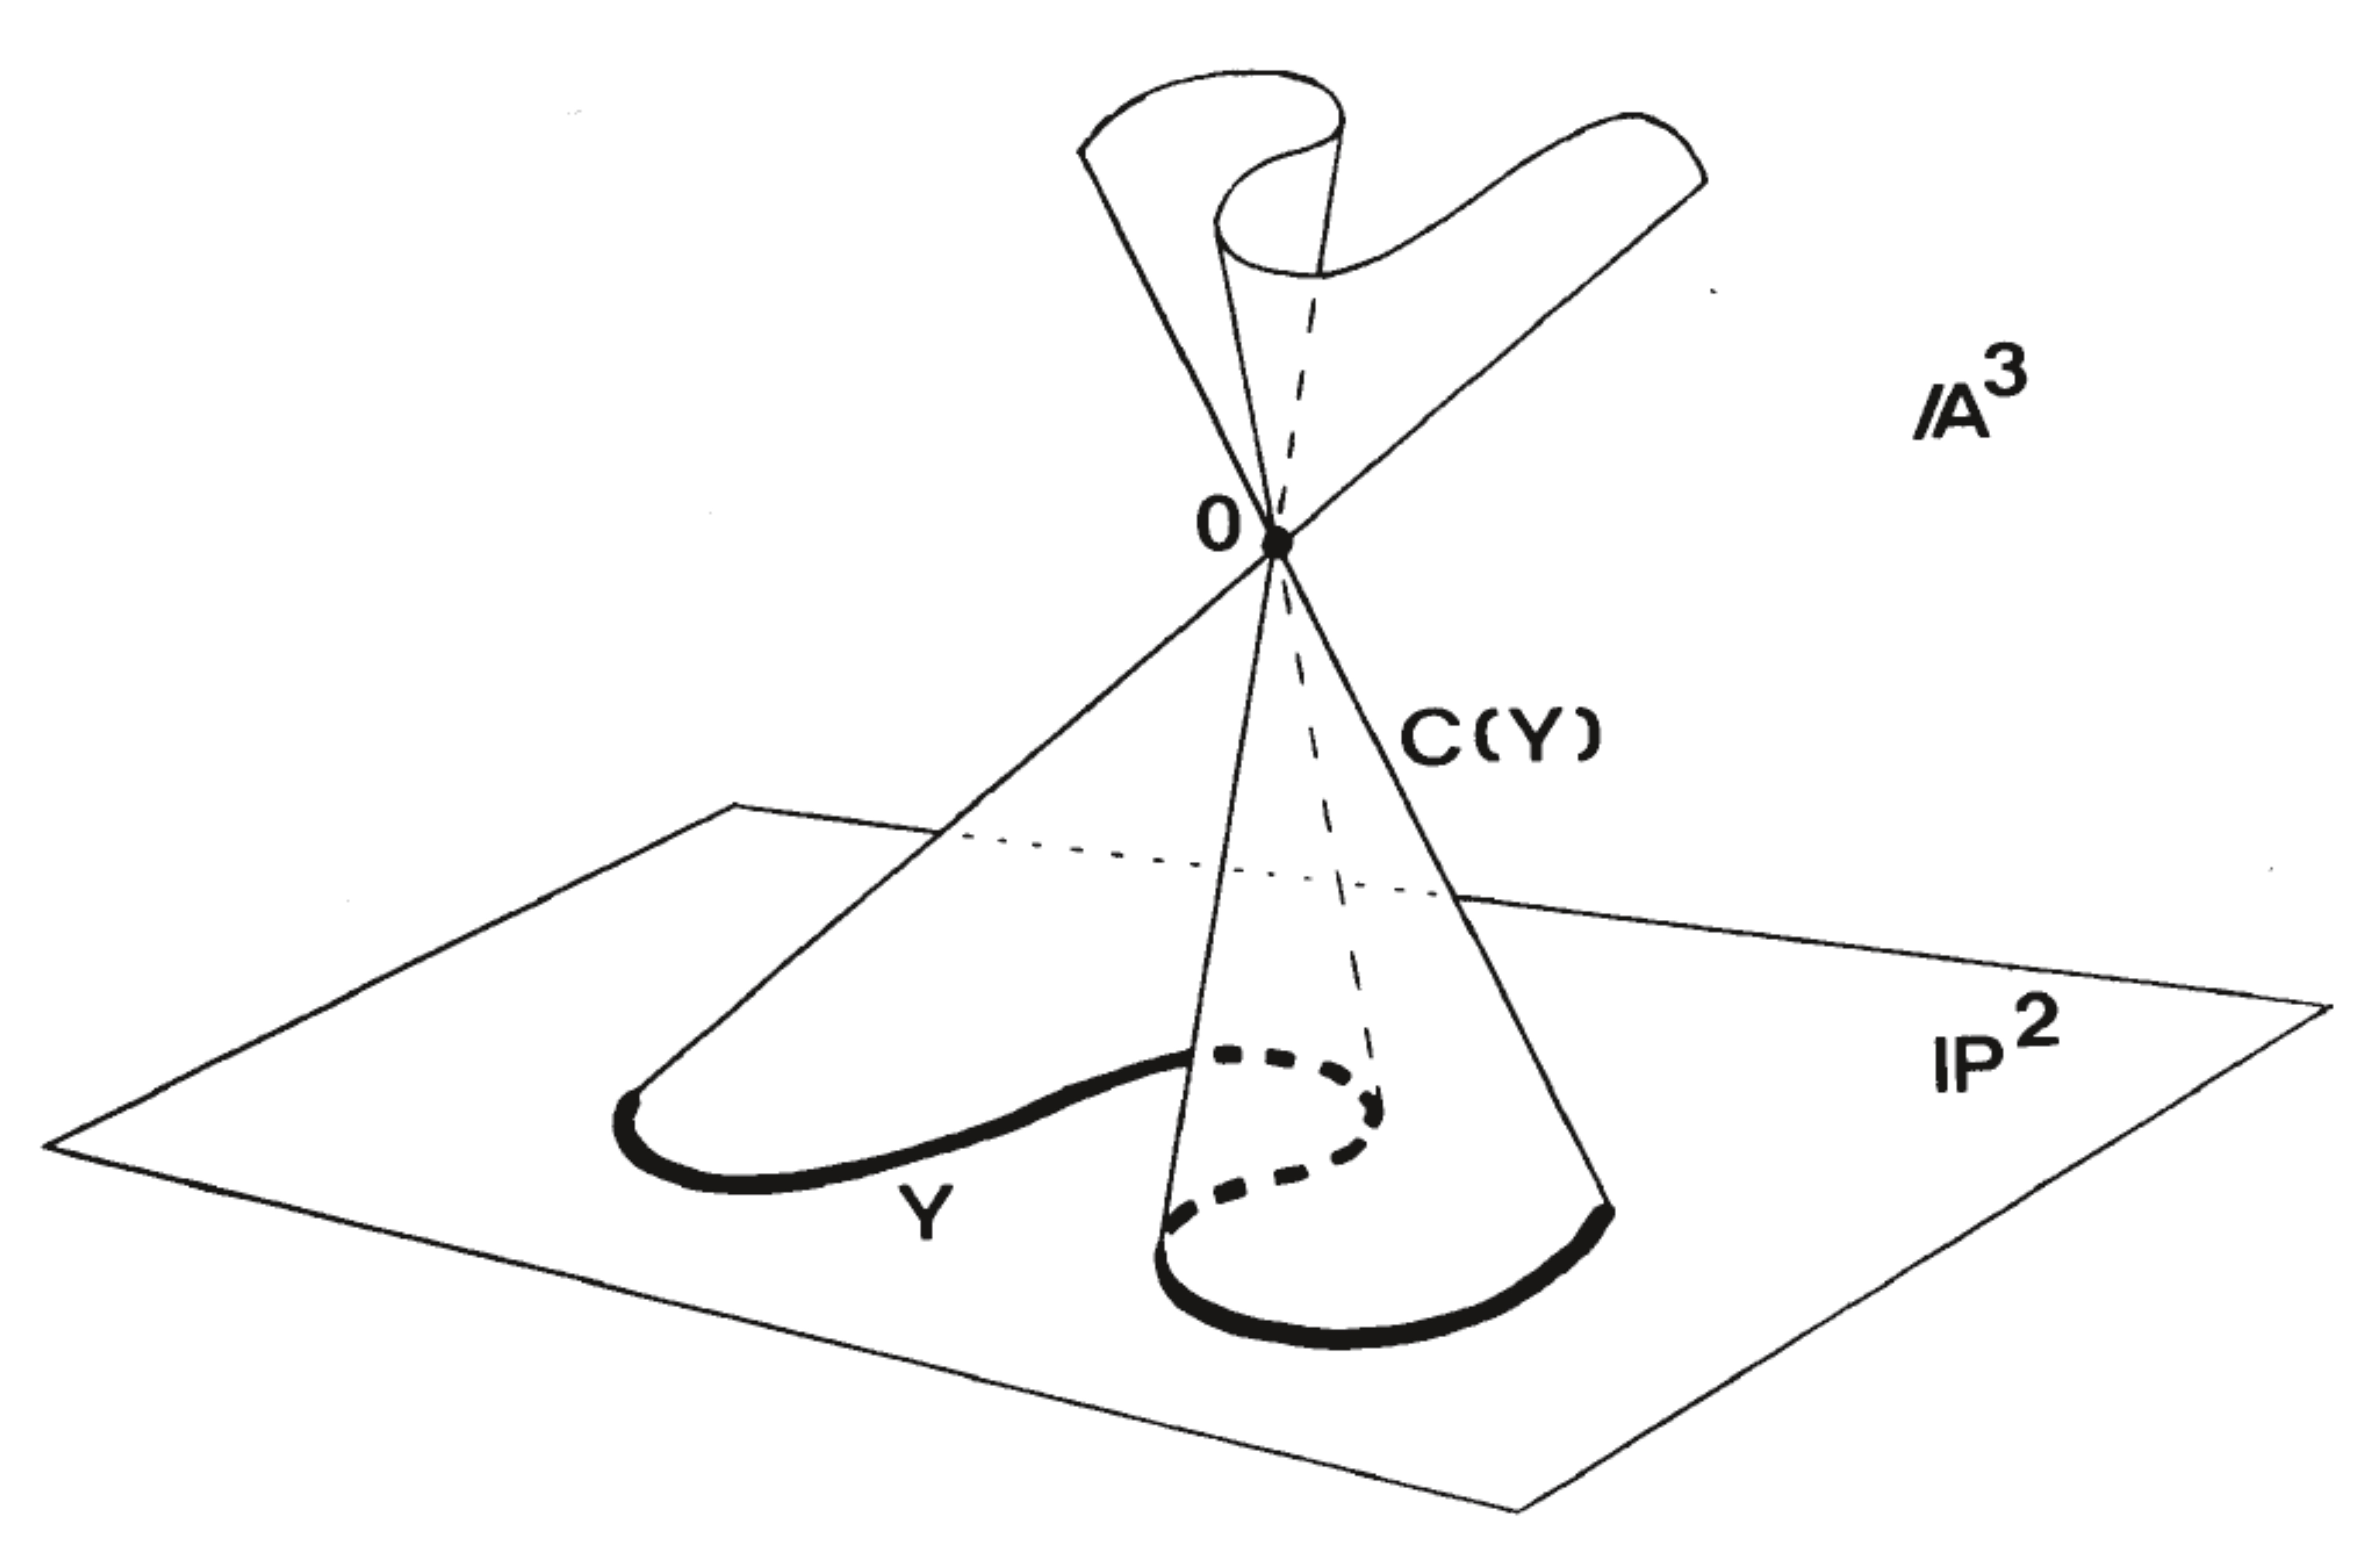
\includegraphics[width=0.5\columnwidth]{Figure1}\\
		Figure 1. $\mb P^2$에서의 곡선 상에서의 뿔
	\end{center}
	%
	\begin{enumerate}[label=\tb{2.\arabic*.},itemindent=0mm,itemsep=2mm]
	\setcounter{enumi}{10}
	\item \tb{$\Pn$에서의 선형 대수다양체}. 1차다항식에 의해 정의된 초곡면은 \tb{초평면(hyperplane)}이라 불린다.
	\begin{enumerate}[label=(\alph*)]
	\item $\Pn$에서의 대수다양체 $Y$에 대한 다음 두 조건이 동치임을 보여라:
	\begin{enumerate}[label=(\roman*)]
	\item $I(Y)$는 1차다항식들에 의해 생성될 수 있다.
	\item $Y$는 초평면들의 교집합으로 표현될 수 있다.
	\end{enumerate}
	이 경우 우리는 $Y$가 $\Pn$에서의 \tb{선형 대수다양체(linear variety)}라 한다.
	\item 만약 $Y$가 $\Pn$에서의 $r$차원 선형 대수다양체이면
	$I(Y)$가 최소 $n-r$개의 1차다항식에 의해 생성됨을 보여라.
	\item $Y,Z$가 $\Pn$에서의 선형 대수다양체이며 $\dim Y=r,\dim Z=s$라 하자.
	만약 $r+s-n\ge 0$이면 $Y\cap Z\ne\es$이다.
	이에 더해 만약 $Y\cap Z\ne\es$이면 $Y\cap Z$는 차원 $r+s-n$ 이상의 선형 대수다양체이다.
	($\mb A^{n+1}$을 $k$ 상에서의 벡터 공간으로 간주하고 그 부분공간에서 작업하라.)
	\end{enumerate}
	\item \tb{$d$차 매장}. 주어진 $n,d>0$에 대하여 $M_0,M_1,\ldots,M_N$이
	$n+1$개 변수 $x_0,\ldots,x_n$에 대한 모든 $d$차 단항식들이라 하자. 여기에서 $N=\binom{n+d}{n}-1$이다.
	함수 $\rho_d:\Pn\ra\mb P^N$을 점 $P=(a_0,\ldots,a_n)$을 단항식 $M_j$들에 $a_i$들을 대입하여 얻어진
	점 $\rho_d(P)=(M_0(a),\ldots,M_N(a))$로 대응시키는 함수로 정의하자.
	이는 $\Pn$에서 $\mb P^N$으로의 \tb{$d$차 매장($d$-uple embedding)}이라 불린다.
	예를 들어 만약 $n=1,d=2$이면 $N=2$이고 $\mb P^1$의 $\mb P^2$로의 $2$차 매장의 상 $Y$는 원뿔곡선이다.
	\begin{enumerate}[label=(\alph*)]
	\item $\ta:k[y_0,\ldots,y_N]\ra k[x_0,\ldots,x_n]$이
	$y_i$를 $M_i$로 대응시키는 것으로 정의된 준동형사상이며 $\mf a$가 $\ta$의 핵이라 하자.
	그 경우 $\mf a$는 동차 소 아이디얼이며 따라서 $Z(\mf a)$는 $\mb P^N$에서의 사영 대수다양체이다.
	\item $\rho_d$의 상이 정확히 $Z(\mf a)$임을 보여라. (한쪽 포함 관계는 간단하다. 반대쪽은 계산이 필요하다.)
	\item 이제 $\rho_d$가 $\Pn$에서 사영 대수다양체 $Z(\mf a)$로의 위상동형사상임을 보여라.
	\item $\mb P^3$에서의 비틀린 3차곡선(Ex. 2.9)이 적절한 좌표 선택 하에서
	$\mb P^1$의 $\mb P^3$으로의 3차 매장과 동일함을 보여라.
	\end{enumerate}
	\item $Y$가 $\mb P^2$의 $\mb P^5$로의 2차 매장의 상이라 하자. 이는 \tb{Veronese 곡면(Veronese surface)}이다.
	만약 $Z\bseq Y$가 폐곡선이면(\tb{곡선(curve)}은 1차원 대수다양체이다)
	$V\cap Y=Z$를 만족시키는 초곡면 $V\bseq\mb P^5$가 존재함을 보여라.
	\item \tb{Segre 매장}. $\psi:\mb P^r\times\mb P^s\ra\mb P^N$이 순서 쌍 $(a_0,\ldots,a_r)\times(b_0,\ldots,b_s)$를
	사전 순서인 $(\ldots,a_ib_j,\ldots)$로 대응시키는 것으로 정의된 함수라 하자. 여기에서 $N=rs+r+s$이다.
	$\psi$가 잘 정의되었으며 단사임을 기억해 두라. 이는 \tb{Segre 매장(Segre embedding)}이라 불린다.
	$\psi$의 상이 $\mb P^N$의 \tb{부분대수다양체(subvariety)}임을 보여라.
	[Hint: $\mb P^N$의 동차 좌표가 $\sx{z_{ij}}{i=0,\ldots,r,j=0,\ldots,s}$라 하고
	$\mf a$가 $z_{ij}$를 $x_iy_j$로 대응시키는 준동형사상 $k[\{z_{ij}\}]\ra k[x_0,\ldots,x_r,y_0,\ldots,y_s]$의 핵이라 하자.
	그 후 $\Im\psi=Z(\mf a)$임을 보여라]
	\item \tb{$\mb P^3$에서의 2차곡면} (Fig. 2). 방정식 $xy-zw=0$에 의해 정의된 $\mb P^3$에서의 곡면 $Q$를 고려하자.
	(\tb{곡면(surface)}은 2차원 대수다양체이다.)
	\begin{enumerate}[label=(\alph*)]
	\item $Q$가 적절한 좌표 선택 하에서 $\mb P^1\times\mb P^1$의 $\mb P^3$으로의 Segre 매장과 동일함을 보여라.
	\item $Q$가 $t\in\mb P^1$에 의해 매개화된 다음을 만족시키는 직선들의 두 개의 족 $\{L_t\},\{M_t\}$를 포함함을 보여라:
	(\tb{직선(line)}은 1차원 선형 대수다양체이다.)
	만약 $L_t\ne L_u$이면 $L_t\cap L_u=\es$, 만약 $M_t\ne M_u$이면 $M_t\cap M_u=\es$,
	모든 $t,u$에 대하여 $L_t\cap M_u=$ 한 점.
	\item $Q$가 이러한 직선들 이외에도 다른 곡선들을 포함함을 보이고 $Q$ 상에서의 Zariski 위상이
	$\mb P^1\times\mb P^1$ 상에서의 곱위상(여기에서 각각의 $\mb P^1$은 Zariski 위상을 가진다.)과
	$\psi$를 통해 위상동형이 아님을 보여라.
	\end{enumerate}
	\end{enumerate}
	%
	%Figure 2
	\begin{center}
	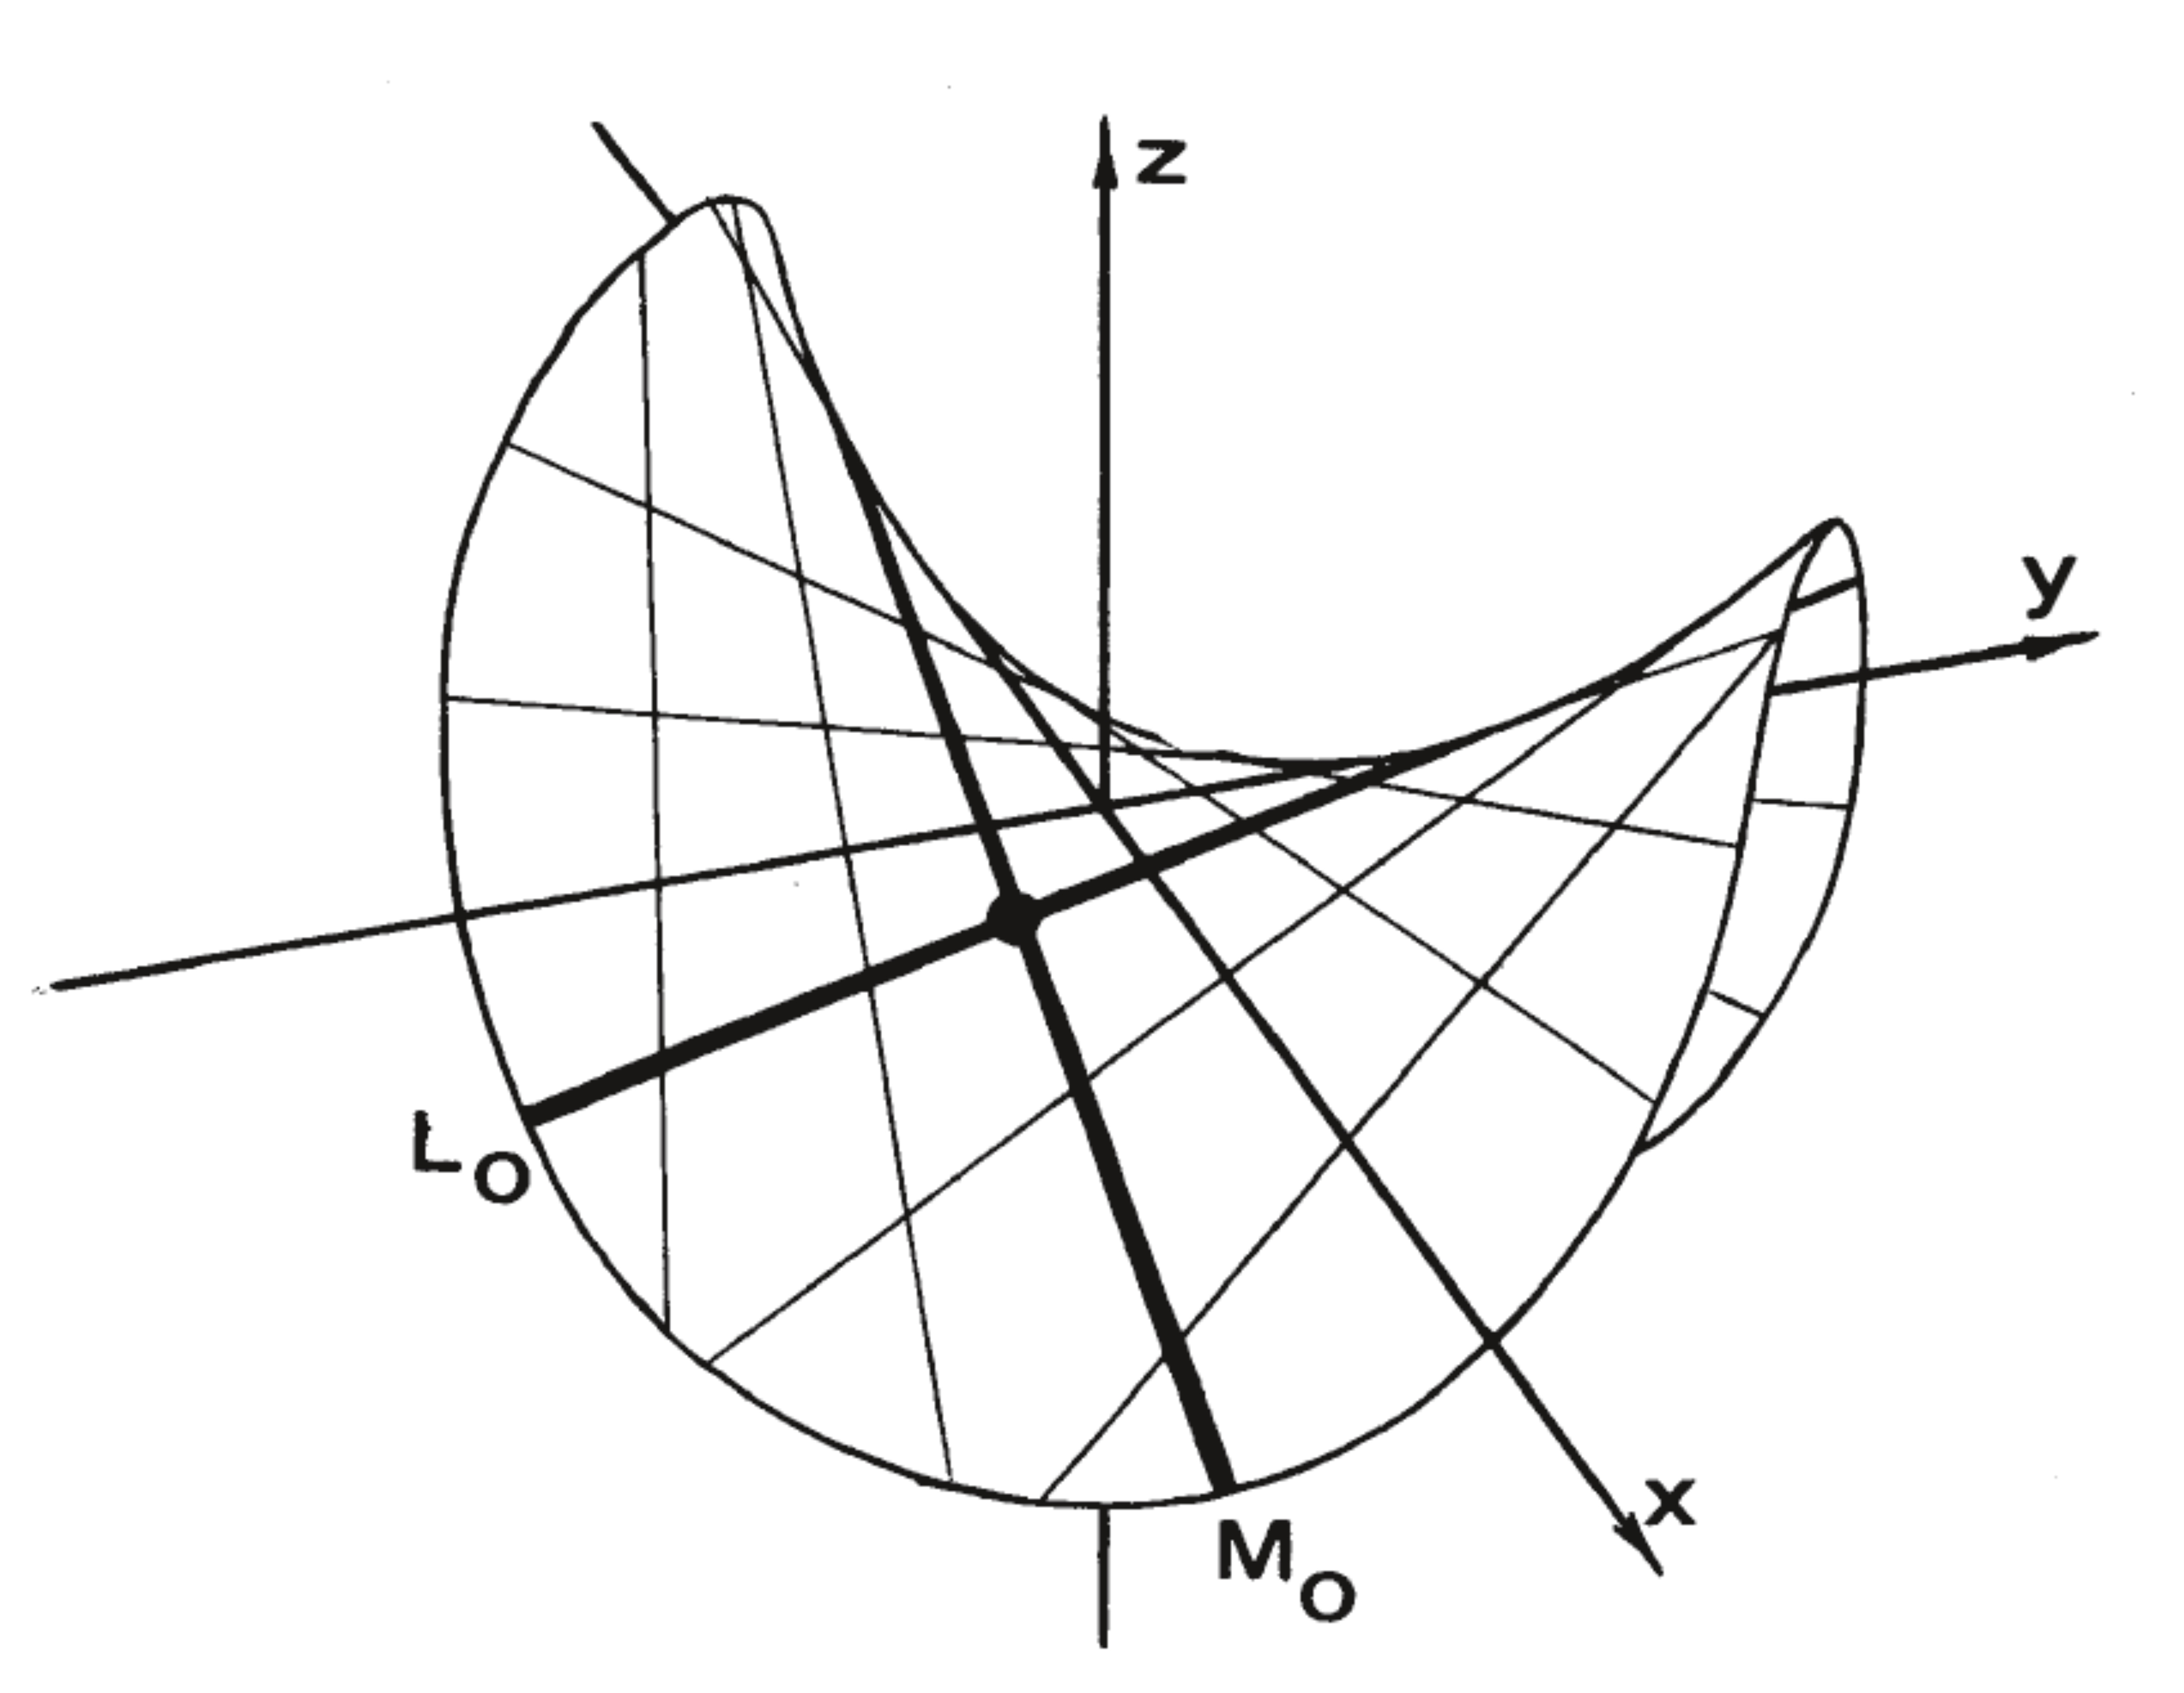
\includegraphics[width=0.5\columnwidth]{Figure2}\\
	Figure 2. $\mb P^3$에서의 2차곡면
	\end{center}
	%
	\begin{enumerate}[label=\tb{2.\arabic*.},itemindent=0mm,itemsep=2mm]
	\setcounter{enumi}{15}
	\item \begin{enumerate}[label=(\alph*)]
	\item 두 대수다양체의 교집합이 대수다양체여야 할 필요는 없다.
	예를 들어 $Q_1$과 $Q_2$가 각각 방정식 $x^2-yw=0$과 $xy-zw=0$에 의해 주어진 $\mb P^3$에서의 2차곡면이라 하자.
	$Q_1\cap Q_2$가 비틀린 3차곡선과 직선의 합집합임을 보여라.
	\item 두 대수다양체의 교집합이 대수다양체이더라도 교집합의 아이디얼은 아이디얼들의 합이 아닐 수 있다.
	예를 들어 $C$가 방정식 $x^2-yz=0$에 의해 주어진 $\mb P^2$에서의 2차곡선이라 하자.
	$L$이 $y=0$에 의해 주어진 직선이라 하자. $C\cap L$이 한 점 $P$로 구성되어 있지만 $I(C)+I(L)\ne I(P)$임을 보여라.
	\end{enumerate}
	\item \tb{완비 교집합}. $\Pn$에서의 $r$차원 대수다양체 $Y$가 \tb{(강)완비 교집합((strict) complete intersection)}이라는
	것의 정의는 $I(Y)$가 $n-r$개 원소에 의해 생성될 수 있는 것이다.
	$Y$가 \tb{집합론적 완비 교집합(set-theoretic complete intersection)}이라는 것의 정의는
	$Y$가 $n-r$개 초곡면의 교집합으로 표현 가능한 것이다.
	\begin{enumerate}[label=(\alph*)]
	\item $Y$가 $\Pn$에서의 대수다양체이며 $Y=Z(\mf a)$라 하자. 또한 $\mf a$가 $q$개 원소에 의해 생성될 수 있다 하자.
	그 경우 $\dim Y\ge n-q$임을 보여라.
	\item 강완비 교집합이 집합론적 완비 교집합임을 보여라.
	\end{enumerate}
	\begin{enumerate}[label=*(\alph*)]
	\setcounter{enumii}{2}
	\item (b)의 역은 거짓이다. 예를 들어 $Y$가 $\mb P^3$에서의 비틀린 3차곡선이라 하자. (Ex. 2.9)
	$I(Y)$가 두 원소에 의해 생성될 수 없음을 보여라.
	반면에 $Y=H_1\cap H_2$를 만족시키는 각각 2차와 3차인 초곡면 $H_1,H_2$를 찾아라.
	\end{enumerate}
	\begin{enumerate}[label=**(\alph*)]
	\setcounter{enumii}{3}
	\item $\mb P^3$에서의 모든 닫힌 기약 곡선이 두 곡면의 집합론적 교집합인지는 아직 해결되지 않은 문제이다.
	해설에 대해서는 Hartshorne [1]과 Hartshorne [5, III, \S 5]를 참조하라.
	\end{enumerate}
	\end{enumerate}
	
	
	
	%Section I.3
	\section{Morphisms (사상)}
	
	지금까지 우리는 아핀 및 사영 대수다양체를 정의했지만 우리는 이들 간에 어떠한 사상이 허용되었는지는 논의하지 않았다.
	우리는 심지어 어떠한 경우에 두 대수다양체가 동형인지도 언급하지 않았다.
	이 절에서 우리는 대수다양체 상에서의 정칙 함수에 대해 논의하고 대수다양체의 사상을 정의할 것이다.
	그러므로 우리는 작업을 수행할 좋은 범주를 얻게 될 것이다.
	
	$Y$가 $\An$에서의 준아핀 대수다양체라 하자. 우리는 $Y$에서 $k$로의 함수 $f$들을 고려할 것이다.
	
	
	%Definition
	\begin{definition}
	%
		\tn{함수 $f:Y\ra k$가 \tb{점 $P\in Y$에서 정칙(regular at a point $P\in Y$)}이라는 것의 정의는
		$P\in U\bseq Y$를 만족시키는 열린 근방 $U$와 다항식 $g,h\in A=k[x_1,\ldots,x_n]$이 존재하여
		$h$가 $U$ 상에서 영점을 갖지 않으며 $U$ 상에서 $f=g/h$인 것이다.
		(여기에서 물론 우리는 다항식을 $\An$ 상에서의 함수로 해석하며 따라서 이는 $Y$ 상에서의 함수이다.)
		$f$가 \tb{$Y$ 상에서 정칙(regular on $Y$)}이라는 것의 정의는 $Y$의 모든 점에서 정칙인 것이다.}
	%
	\end{definition}
	
	
	%Lemma 3.1
	\begin{lemma}
	%
		\tn{\\$k$가 Zariski 위상을 가지는 $\mb A_k^1$과 동일시될 경우 정칙 함수는 연속이다.\\\\
	%
		\pf 닫힌집합의 $f$에 의한 역상이 닫힌집합임을 보이면 충분하다.
		$\mb A_k^1$의 닫힌집합들은 유한 개 점들이므로
		임의의 $a\in k$에 대하여 $f^{-1}(a)=\sx{P\in Y}{f(P)=a}$가 닫혀 있음을 보이면 충분하다.
		이는 국소적으로 확인될 수 있다: 위상공간 $Y$의 부분집합 $Z$가 닫혀 있을 필요충분조건은
		$Z\cap U$가 $U$에서 닫혀 있도록 하는 열린 부분집합 $U$들에 의해 $Y$가 덮일 수 있는 것이다.
		그러므로 $U$가 $f$가 $g,h\in A$에 대하여 $g/h$로 표현될 수 있으며 $h$가 $U$ 상에서 영점을 갖지 않도록 하는 열린집합이라 하자.
		그 경우 $f^{-1}(a)\cap U=\sx{P\in U}{g(P)/h(P)=a}$이다.
		그러나 $g(P)/h(P)=a$ iff $(g-ah)(P)=0$이다. 그러므로 $f^{-1}(a)\cap U=Z(g-ah)\cap U$이며 이는 닫힌집합이다.
		따라서 $f^{-1}(a)$는 $Y$에서 닫혀 있다.}
	%
	\end{lemma}
	
	이제 준사영 대수다양체 $Y\bseq\Pn$을 고려하자.
	
	
	%Definition
	\begin{definition}
	%
		\tn{함수 $f:Y\ra k$가 \tb{점 $P\in Y$에서 정칙(regular at a point $P\in Y$)}이라는 것의 정의는
		$P\in U\bseq Y$를 만족시키는 열린 근방 $U$와 같은 차수의 동차다항식 $g,h\in A=k[x_0,\ldots,x_n]$이 존재하여
		$h$가 $U$ 상에서 영점을 갖지 않으며 $U$ 상에서 $f=g/h$인 것이다.
		(이 경우 $g$와 $h$가 $\Pn$ 상에서의 함수가 아님에도 불구하고 이들이 같은 차수의 동차다항식이므로
		$h\ne 0$이면 이들의 몫이 잘 정의됨을 기억해 두라.)
		$f$가 \tb{$Y$ 상에서 정칙(regular on $Y$)}이라는 것의 정의는 $Y$의 모든 점에서 정칙인 것이다.}
	%
	\end{definition}
	
	
	%Remark 3.1.1
	\begin{remark}
	%
		\tn{\\준아핀 경우와 마찬가지로 정칙 함수는 반드시 연속해야 한다. (증명은 독자에게 남긴다.)
		이것의 중요한 결과는 만약 $f$와 $g$가 대수다양체 $X$ 상에서의 정칙 함수들이며
		어떠한 공집합이 아닌 열린 부분집합 $U\bseq X$ 상에서 $f=g$이면 모든 곳에서 $f=g$라는 것이다:
		$f-g=0$인 점들의 집합은 닫힌 조밀 집합이므로 $X$와 같다.}
	%
	\end{remark}
	
	이제 우리는 대수다양체의 범주를 정의할 수 있다.
	
	
	%Definition
	\begin{definition}
	%
		\tn{$k$가 고정된 대수적으로 닫힌 체라 하자. \tb{$k$ 상에서의 대수다양체(variety over $k$)}%
		(또는 간단히 \tb{대수다양체(variety)})는 위에서 정의한 임의의 아핀, 준아핀, 사영, 준사영 대수다양체이다.
		만약 $X,Y$가 두 대수다양체이면 \tb{사상(morphism)} $\ph:X\ra Y$는 모든 열린집합 $V\bseq Y$와
		임의의 정칙 함수 $f:V\ra k$에 대하여 함수 $f\circ\ph:\ph^{-1}(V)\ra k$가 정칙이도록 하는 연속 함수이다.}
	%
	\end{definition}
	
	명백히 두 사상의 합성은 사상이며 따라서 우리는 범주를 얻는다. 특히 동형사상의 개념을 얻는다:
	두 대수다양체 간의 \tb{동형사상(isomorphism)} $\ph:X\ra Y$는 $\psi\circ\ph=\id_X$와 $\ph\circ\psi=\id_Y$를 만족시키는
	역사상 $\psi:Y\ra X$를 가지는 사상이다.
	동형사상은 반드시 전단사이며 쌍연속이어야 하지만 전단사 쌍연속 사상이 동형사상이어야 할 필요는 없음을 기억해 두라. (Ex. 3.2)\\
	
	이제 우리는 임의의 대수다양체에 연관된 어떠한 함수들의 환을 도입할 것이다.
	
	
	%Definition
	\begin{definition}
	%
		\tn{$Y$가 대수다양체라 하자. $Y$ 상에서의 모든 정칙 함수들의 환을 $\mc O(Y)$로 표기한다.
		만약 $P$가 $Y$에서의 점이면 \tb{$P$의 $Y$ 상에서의 국소환(local ring of $P$ on $Y$)}
		$\mc O_{P,Y}$(또는 간단히 $\mc O_P$)를 $P$ 근처에서 $Y$ 상에서의 정칙 함수들의 \tb{싹(germ)}들의 환으로 정의한다.
		다른 말로 하면 $\mc O_P$의 원소는 $P$를 포함하는 $Y$의 열린 부분집합 $U$와 $U$ 상에서의 정칙 함수 $f$의 쌍 $\bk{U,f}$이며
		$U\cap V$ 상에서 $f=g$일 경우 두 쌍 $\bk{U,f}$와 $\bk{V,g}$를 동일시한다.
		(이것이 동치 관계임을 검증하기 위해 (3.1.1)을 사용하라.)}
	%
	\end{definition}
	
	$\mc O_P$가 실제로 국소환임을 기억해 두라: 그 극대 아이디얼 $\mf m$은 $P$에서 소멸하는 정칙 함수들의 싹들의 집합이다.
	(만약 $f(P)\ne 0$이면 $1/f$는 $P$의 어떠한 근방에서 정칙이다.)
	잉여류체 $\mc O_P/\mf m$은 $k$와 동형이다.
	
	
	%Definition
	\begin{definition}
	%
		\tn{만약 $Y$가 대수다양체이면 $Y$의 \tb{함수체(function field)} $K(Y)$를 다음과 같이 정의한다:
		$K(Y)$의 원소는 $Y$의 공집합이 아닌 열린 부분집합 $U$와 $U$ 상에서의 정칙 함수 $f$의 쌍 $\bk{U,f}$의 동치류들이다;
		만약 $U\cap V$ 상에서 $f=g$이면 두 쌍 $\bk{U,f}$와 $\bk{V,g}$를 동일시한다.
		$K(Y)$의 원소들은 $Y$ 상에서의 \tb{유리함수(rational function)}들이라 불린다.}
	%
	\end{definition}
	
	$K(Y)$가 실제로 체임을 기억해 두라. $Y$가 기약이므로 임의의 두 공집합이 아닌 열린집합은 공집합이 아닌 교집합을 가진다.
	따라서 우리는 $K(Y)$에서 덧셈과 곱셈을 정의할 수 있으며 $K(Y)$는 환이 된다.
	그 경우 만약 $\bk{U,f}\in K(Y)$이며 $f\ne 0$이면 우리는 $f$를 열린집합 $V=U-U\cap Z(f)$로 제한할 수 있으며
	이곳에서 $f$는 영점을 갖지 않고 따라서 $1/f$는 $V$ 상에서 정칙이며 $\bk{V,1/f}$는 $\bk{U,f}$의 역이다.
	
	지금까지 우리는 임의의 대수다양체 $Y$에 대하여 대역적 함수들의 환 $\mc O(Y)$,
	$Y$의 점에서의 국소환 $\mc O_P$, 함수체 $K(Y)$를 정의했다.
	함수의 제한에 의해 우리는 자연스러운 함수 $\mc O(Y)\ra\mc O_P\ra K(Y)$를 얻는다.
	(3.1.1)에 의해 이는 사실 단사이다.
	따라서 우리는 통상적으로 $\mc O(Y)$와 $\mc O_P$를 $K(Y)$의 부분환으로 취급할 것이다.
	
	만약 우리가 $Y$를 동형인 대수다양체로 대체한다면 대응하는 환들은 동형이다.
	그러므로 우리는 $\mc O(Y)$, $\mc O_P,K(Y)$가 대수다양체 $Y$(와 점 $P$)의 동형 하에서의 \tb{불변량(invariant)}이라 말할 수 있다.
	
	우리의 다음 작업은 $\mc O(Y),\mc O_P,K(Y)$를 앞에서 도입한
	아핀 대수다양체의 아핀 좌표환 $A(Y)$/사영 대수다양체의 동차 좌표환 $S(Y)$와 연관짓는 것이다.
	우리는 아핀 대수다양체 $Y$에 대하여 $A(Y)=\mc O(Y)$이며 따라서 이것이 동형 하에서 불변임을 보일 것이다.
	그러나 사영 대수다양체 $Y$에서 $S(Y)$는 불변이 아니다: 이는 $Y$의 사영공간으로의 매장에 의존한다. (Ex. 3.9)
	
	
	%Theorem 3.2
	\begin{theorem}
	%
		\tn{\\$Y\bseq\An$이 아핀 좌표환 $A(Y)$를 가지는 아핀 대수다양체라 하자. 그 경우 다음이 성립한다:\\[-2mm]
	%
		\begin{enumerate}[label=(\alph*)]
		\item $\mc O(Y)\cong A(Y)$
		\item 각각의 점 $P\in Y$에 대하여 $\mf m_p\bseq A(Y)$가 $P$에서 소멸하는 함수들의 아이디얼이라 하자.
		그 경우 $P\mt\mf m_P$는 $Y$의 점과 $A(Y)$의 극대 아이디얼 간의 일대일 대응을 제공한다.
		\item 각각의 $P$에 대하여 $\mc O_P\cong A(Y)_{\mf m_P}$이며 $\dim\mc O_P=\dim Y$이다.
		\item $K(Y)$는 $A(Y)$의 분수체와 동형이며 따라서 $K(Y)$는 초월 차수가 $\dim Y$인 $k$의 유한생성 확대체이다.
		\end{enumerate}}
	%
		\tn{\\\pf 여러 단계로 진행할 것이다. 먼저 함수 $\al:A(Y)\ra\mc O(Y)$를 정의할 것이다.
		모든 다항식 $f\in A=k[x_1,\ldots,x_n]$은 $\An$ 상에서의 하나의 정칙 함수를 정의하며 따라서 $Y$ 상에서도 그러하다.
		그러므로 우리는 준동형사상 $A\ra\mc O(Y)$를 얻는다.
		그 핵은 $I(Y)$이며 따라서 우리는 단사 준동형사상 $\al:A(Y)\ra\mc O(Y)$를 얻는다.\\
		(1.4)에 의해 우리는 $Y$의 점($Y$의 극소 대수적 부분집합들)과 $I(Y)$를 포함하는 $A$의 극대 아이디얼 간에
		일대일 대응관계가 존재함을 안다. $I(Y)$에 대한 몫을 취하면 이는 $A(Y)$의 극대 아이디얼에 대응한다.
		이에 더해 $\al$를 사용해 $A(Y)$의 원소를 $Y$ 상에서의 정칙 함수와 동일시하면
		$P$에 대응하는 극대 아이디얼은 $\mf m_P=\sx{f\in A(Y)}{f(P)=0}$이다. 이는 (b)를 증명한다.\\
		각각의 $P$에 대하여 자연스러운 함수 $A(Y)_{\mf m_P}\ra\mc O_P$가 존재한다.
		$\al$가 단사이므로 이는 단사이며, 정칙 함수의 정의에 의해 이는 전사이다.
		이는 $\mc O_P\cong A(Y)_{\mf m_P}$임을 보여준다. 이제 $\dim\mc O_P=\mrm{height}\;\mf m_P$이다.
		$A(Y)/\mf m_P\cong k$이므로 (1.7)과 (1.8A)에 의해 $\dim\mc O_P=\dim Y$라 결론지을 수 있다.\\
		(c)로부터 모든 $P$에 대하여 $A(Y)$의 분수체가 $\mc O_P$의 분수체와 동형임이 따라온다.
		모든 유리함수는 실제로 어떠한 $\mc O_P$에 속하므로 이는 $K(Y)$와 같다.
		이제 $A(Y)$가 유한생성 $k$-대수이므로 $K(Y)$는 $k$의 유한생성 확대체이다.
		이에 더해 (1.7)과 (1.8A)에 의해 초월 차수 $K(Y)/k$는 $\dim Y$와 같다. 이는 (d)를 증명한다.\\
		(a)를 증명하기 위해 (모든 환이 $K(Y)$의 부분환으로 간주된 경우) $O(Y)\bseq\bigcap_{P\in Y}\mc O_P$임을 기억해 두라.\\
		(b)와 (c)를 이용하면 다음을 얻는다.}
	%
		$$A(Y)\bseq\mc O(Y)\bseq\bigcap_{\mf m}A(Y)_{\mf m}$$
	%
		\tn{여기에서 $\mf m$이 $A(Y)$의 임의의 극대 아이디얼인 경우에 대하여 교집합을 취한다.
		이제 만약 $B$가 정역이면 $B$는 모든 극대 아이디얼에서의 국소화들의 (분수체 내에서의) 교집합과 같다는
		간단한 대수적 사실로부터 등식이 따라온다.}
	%
	\end{theorem}
	
	
	%Proposition 3.3
	
	\begin{proposition}
	%
		\tn{\\$U_i\bseq\Pn$이 방정식 $x_i\ne 0$에 의해 정의된 열린집합이라 하자.
		그 경우 (2.2)의 함수 $\ph_i:U_i\ra\An$은 대수다양체 동형사상이다.\\\\
	%
		\pf 우리는 이미 이것이 위상동형사상임을 보였으므로 두 열린집합 상에서 정칙 함수들이 동일함을 확인하면 충분하다.
		$U_i$ 상에서 정칙 함수들은 국소적으로 $x_0,\ldots,x_n$에 대한 같은 차수의 동차다항식들의 몫이다.
		$\An$ 상에서 정칙 함수들은 국소적으로 $y_1,\ldots,y_n$에 대한 다항식들의 몫이다.
		(2.2)의 증명의 함수 $\al$와 $\be$에 의해 이러한 두 개념이 동일시될 수 있음을 간단히 확인할 수 있다.}
	%
	\end{proposition}
	
	다음 결과를 시작하기 전에 표기법을 도입하겠다.
	만약 $S$가 등급환이며 $\mf p$가 $S$에서의 동급 소 아이디얼이면 $\mf p$에 속하지 않은 $S$의 동급 원소들로 구성된
	곱셈적 부분집합 $T$에 대한 $S$의 국소화에서 차수가 0인 원소들의 부분환을 $S_{(\mf p)}$로 나타낸다.
	$T^{-1}S$는 $S$에서 동급인 $f$와 $g\in T$에 대하여 $\deg(f/g)=\deg f-\deg g$에 의해 주어진 자연스러운 등급을 가진다.
	$S_{(\mf p)}$는 극대 아이디얼 $(\mf p\cdot T^{-1}S)\cap S_{(\mf p)}$를 가지는 국소환이다.
	특히 만약 $S$가 정역이면 $\mf p=(0)$에 대하여 우리는 체 $S_{((0))}$을 얻는다.
	마찬가지로 만약 $f\in S$가 동급 원소이면 국소환 $S_f$에서의 차수 0인 원소들의 부분환을 $S_{(f)}$로 표기한다.
	
	
	%Theorem 3.4
	\begin{theorem}
	%
		\tn{\\$Y\bseq\Pn$이 동차 좌표환 $S(Y)$를 가지는 사영 대수다양체라 하자. 그 경우 다음이 성립한다:\\[-2mm]
	%
		\begin{enumerate}[label=(\alph*)]
		\item $\mc O(Y)=k$
		\item 임의의 점 $P\in Y$에 대하여 $\mf m_P\bseq S(Y)$가 $f(P)=0$을 만족시키는
		동차 $f\in S(Y)$들의 집합에 의해 생성된 아이디얼이라 하자. 그 경우 $\mc O_P=S(Y)_{(\mf m_P)}$이다.
		\item $K(Y)\cong S(Y)_{((0))}$
		\end{enumerate}}
	%
		\tn{\\\pf 시작하기 전에 $U_i\bseq\Pn$이 열린집합 $x_i\ne 0$이며 $Y_i=Y\cap U_i$라 하자.
		그 경우 $U_i$는 (3.3)의 동형사상 $\ph_i$에 의해 $\An$과 동형이다.
		그러므로 우리는 $Y_i$를 아핀 대수다양체로 간주할 수 있다.
		아핀 좌표환 $A(Y_i)$와 $Y$의 동차 좌표환의 국소화 $S(Y)_{(x_i)}$ 간에는 자연스러운 동형사상 $\ph_i^*$가 존재한다:
		우리는 먼저 (2.2)의 증명에서와 같이 $f(y_1,\ldots,y_n)$을 $f(x_0/x_i,\ldots,x_n/x_i)$($x_i/x_i$ 제외)로 사상하는
		$k[y_1,\ldots,y_n]$과 $k[x_0,\ldots,x_n]_{(x_i)}$ 간의 동형사상을 도입할 것이다.
		이 동형사상은 $I(Y_i)$를 $I(Y)S_{(x_i)}$로 사상한다. (cf. Ex. 2.6)
		그러므로 몫을 거치면 우리는 요구된 동형사상 $\ph_i^*:A(Y_i)\cong S(Y)_{(x_i)}$를 얻는다.\\
		이제 (b)를 증명하기 위해 $P\in Y$가 임의의 점이라 하고 $i$를 $P\in Y_i$이도록 선택하자.
		그 경우 (3.2)에 의해 $\mf m_P'$가 $P$에 대응하는 $A(Y_i)$의 극대 아이디얼이라 하면 $\mc O_P\cong A(Y_i)_{\mf m_P'}$이다.
		$\ph_i^*(\mf m_P')=\mf m_P\cdot S(Y)_{(x_i)}$임을 간단히 확인할 수 있다.
		이제 $x_i\notin\mf m_P$이며 국소화가 추이적이므로
		$A(Y_i)_{\mf m_P'}\cong S(Y)_{(\mf m_P)}$임을 알아낼 수 있으며 이는 (b)를 증명한다.\\
		(c)를 증명하기 위해 우리는 (3.2)를 다시 사용하여 $K(Y)$가 $K(Y_i)$와 같으며 이것이 $A(Y_i)$의 분수체임을 보일 것이다.
		그러나 $\ph_i^*$에 의해 이는 $S(Y)_{((0))}$과 동형이다.\\
		(a)를 증명하기 위해 $f\in\mc O(Y)$가 대역적 정칙 함수라 하자.
		그 경우 각각의 $i$에 대하여 $f$는 $Y_i$ 상에서 정칙이며 따라서 (3.2)에 의해 $f\in A(Y_i)$이다.
		그러나 우리는 $A(Y)\cong S(Y)_{x_i}$임을 보였으므로 $f$가 $N_i$차 동차 $g_i\in S(Y)$에 대하여
		$g_i/x_i^{N_i}$ 형태로 표현 가능하다 결론지을 수 있다.
		$\mc O(Y),K(Y),S(Y)$를 모두 $S(Y)$의 분수체 $L$의 부분환들로 간주하면
		이는 각각의 $i$에 대하여 $x_i^{N_i}f\in S(Y)_{N_i}$임을 나타낸다.
		이제 $N\ge\sum N_i$를 선택하자. 그 경우 $S(Y)_N$은 $k$-벡터 공간으로서
		$x_0,\ldots,x_n$에 대한 $N$차 단항식들에 의해 선형생성된다. 그러므로 $S(Y)_N\cdot f\bseq S(Y)_N$을 얻는다.
		반복적용하면 모든 $q>0$에 대하여 $S(Y)_N\cdot f^q\bseq S(Y)$를 얻는다. 특히 모든 $q>0$에 대하여 $x_0^Nf^q\in S(Y)$이다.
		이는 $L$의 부분환 $S(Y)[f]$가 유한생성 $S(Y)$-모듈 $x_0^{-N}S(Y)$에 포함됨을 보여준다.
		$S(Y)$가 Noether 환이므로 $S(Y)[f]$는 유한생성 $S(Y)$-모듈이며 따라서 $f$는 $S(Y)$ 상에서 \tb{정수적(integral)}이다.
		(e.g. Atiyah-Macdonald [1, p. 59]를 참조하라.)
		이는 원소 $a_1,\ldots,a_m\in S(Y)$가 존재하여 다음을 만족시킴을 의미한다.}
	%
		$$f^m+a_1f^{m-1}+\cdots+a_m=0$$
	%
		\tn{$f$가 0차이므로 $a_i$를 그 0차 동차 성분으로 대체하더라도 여전히 유효한 방정식이다.
		그러나 $S(Y)_0=k$이므로 $a_i\in k$와 $f$는 $k$ 상에서 대수적이다.
		$k$가 대수적으로 닫혀 있으므로 $f\in k$이며 이는 증명을 완료한다.}
	%
	\end{theorem}
	
	다음 결과는 만약 $X$와 $Y$가 아핀 대수다양체이면 $X$가 $Y$와 동형일 필요충분조건은
	$A(X)$와 $A(Y)$가 $k$-대수로서 동형인 것임을 보여준다.
	사실 증명은 이보다 더 나아가며 따라서 우리는 더 강한 결과를 기술한다.
	
	
	%Proposition 3.5
	\begin{proposition}
	%
		\tn{\\$X$가 임의의 대수다양체이며 $Y$가 아핀 대수다양체라 하자.
		그 경우 다음과 같은 자연스러운 집합론적 전단사 함수가 존재한다.}
	%
		$$\al:\Hom(X,Y)\cong\Hom(A(Y),\mc O(X))$$
	%
		\tn{여기에서 좌측의 $\Hom$은 대수다양체의 사상들을, 우측의 $\Hom$은 $k$-대수 준동형사상들을 의미한다.\\\\
	%
		\pf 사상 $\ph:X\ra Y$가 주어졌다면 $\ph$는 $Y$ 상에서의 정칙 함수들을 $X$ 상에서의 정칙 함수들로 대응시킨다.
		따라서 $\ph$는 $\mc O(Y)$에서 $\mc O(X)$로의 함수를 유도하며 이는 명백히 $k$-대수 준동형사상이다.
		그러나 (3.2)에서 $\mc O(Y)\cong A(Y)$임을 보였으므로 우리는 준동형사상 $A(Y)\ra\mc O(X)$를 얻는다. 이는 $\al$를 정의한다.\\
		역으로 $k$-대수 준동형사상 $h:A(Y)\ra\mc O(X)$가 주어졌다 하자.
		$Y$가 $\An$의 닫힌 부분집합이며 따라서 $A(Y)=k[x_1,\ldots,x_n]/I(Y)$라 가정하자.
		$\bar x_i$가 $x_i$의 $A(Y)$에서의 상이라 하고 원소 $\xi_i=h(\bar x_i)\in\mc O(X)$들을 고려하자.
		이들은 $X$에 대한 대역적 함수이므로 우리는 이들을 이용하여
		함수 $\psi:X\ra\An$을 $P\in X$에 대하여 $\psi(P)=(\xi_i(P),\ldots,\xi_n(P))$로 정의할 수 있다.\\
		다음으로 $\psi$의 상이 $Y$에 포함됨을 보이겠다.
		$Y=Z(I(Y))$이므로 임의의 $P\in X$와 임의의 $f\in I(Y)$에 대하여 $f(\psi(P))=0$임을 보이면 충분하다. 그러나 다음과 같다.}
	%
		$$f(\psi(P))=f(\xi_1(P),\ldots,\xi_n(P))$$
	%
		\tn{이제 $f$가 다항식이고 $h$가 $k$-대수 준동형사상이며 $f\in I(Y)$이므로 다음이 성립한다.}
	%
		$$f(\xi_1(P),\ldots,\xi_n(P))=h(f(\bar x_1,\ldots,\bar x_n))(P)=0$$
	%
		\tn{그러므로 $\psi$는 $X$에서 $Y$로의 함수를 정의하며 이는 주어진 준동형사상 $h$를 유도한다.\\
		증명을 완료하기 위해 우리는 $\psi$가 사상임을 보여야 한다. 이는 다음 보조정리의 결과이다.}
	%
	\end{proposition}
	
	
	%Lemma 3.6
	\begin{lemma}
	%
		\tn{\\$X$가 임의의 대수다양체이며 $Y\bseq\An$이 아핀 대수다양체라 하자.
		집합론적 함수 $\psi:X\ra Y$가 사상일 필요충분조건은 각각의 $i$에 대하여 $x_i\circ\psi$가 $X$ 상에서의 정칙 함수인 것이다.
		(여기에서 $x_1,\ldots,x_n$은 $\An$ 상에서의 좌표함수들이다.)\\\\
	%
		\pf 만약 $\psi$가 사상이면 사상의 정의에 의해 $x_i\circ\psi$는 정칙 함수여야 한다. 역으로 $x_i\circ\psi$가 정칙이라 하자.
		그 경우 임의의 다항식 $f=f(x_1,\ldots,x_n)$에 대하여 $f\circ\psi$도 $X$ 상에서 정칙이다.
		$Y$의 닫힌집합들이 다항함수의 소멸에 의해 정의되며 정칙 함수들이 연속하므로
		우리는 $\psi^{-1}$이 닫힌집합들을 닫힌집합으로 대응시킴을 알 수 있으며 따라서 $\psi$는 연속하다.
		마지막으로 $Y$의 열린 부분집합 상에서의 정칙 함수들은 국소적으로 다항식의 몫이므로
		$Y$의 임의의 열린 부분집합 상에서의 임의의 정칙 함수 $g$에 대하여 $g\circ\psi$는 정칙이다. 따라서 $\psi$는 사상이다.}
	%
	\end{lemma}
	
	
	%Corollary 3.7
	\begin{corollary}
	%
		\tn{\\만약 $X,Y$가 아핀 대수다양체이면 $X$와 $Y$가 동형일 필요충분조건은 $A(X)$와 $A(Y)$가 $k$-대수로서 동형인 것이다.\\\\
	%
		\pf 명제의 직접적인 결과이다.}
	%
	\end{corollary}
	
	범주론의 언어로 위 결과를 다음과 같이 표현 가능하다:
	
	
	%Corollary 3.8
	\begin{corollary}
	%
		\tn{\\함자 $X\mt A(X)$는 $k$ 상에서의 아핀 대수다양체의 범주와 $k$ 상에서의 유한생성 정역의 범주 간의 반변 동치를 유도한다.}
	%
	\end{corollary}
	
	여기에 연습문제에서 사용될 대수적 결과를 포함시키겠다.
	
	
	%Theorem 3.9A
	\begin{theorema}[Finiteness of Integral Closure (정수적 폐포의 유한성)]
	%
		\tn{\\$A$가 체 $k$ 상에서의 유한생성 대수인 정역이라 하자. $K$가 $A$의 분수체이며 $L$이 $K$의 유한 대수적 확대체라 하자.
		그 경우 $A$의 $L$에서의 정수적 폐포 $A'$은 유한생성 $A$-모듈이며 동시에 유한생성 $k$-대수이다.\\\\
	%
		\pf Zariski-Samuel [1, vol. 1, Ch. V., Thm. 9, p. 267]}
	%
	\end{theorema}
	
	
	
	%Exercises
	\subsection*{Exercises (연습문제)}
	
	\begin{enumerate}[label=\tb{3.\arabic*.},itemindent=0mm,itemsep=2mm]
	\item \begin{enumerate}[label=(\alph*)]
	\item $\mb A^2$에서의 임의의 원뿔곡선이 $\mb A^1$ 또는 $\mb A^1-\{0\}$과 동형임을 보여라. (cf. Ex. 1.1)
	\item $\mb A^1$이 자신의 임의의 열린 진부분집합과 동형이 \ti{아님}을 보여라.
	(이 결과는 아래의 Ex. 6.7)에서 일반화된다.
	\item $\mb P^2$에서의 임의의 원뿔곡선은 $\mb P^1$과 동형이다.
	\item 우리는 나중에 (Ex. 4.8) 임의의 두 곡선이 위상동형임을 보일 것이다.
	그러나 $\mb A^2$는 심지어 $\mb P^2$와도 위상동형이 아님을 보여라.
	\item 만약 아핀 대수다양체가 사영 대수다양체와 동형이면 이는 한 점으로만 구성됨을 보여라.
	\end{enumerate}
	\item 기반 함수가 위상 공간 간의 위상동형인사상인 사상은 동형사상일 필요가 없다.
	\begin{enumerate}[label=(\alph*)]
	\item 예를 들어 $\ph:\mb A^1\ra\mb A^2$가 $t\mt(t^2,t^3)$으로 정의되었다 하자.
	$\ph$가 $\mb A^1$에서 곡선 $y^2=x^3$으로의 전단사 쌍연속 사상을 정의하지만 동형사상은 아님을 보여라.
	\item 다른 예를 위해, 기반체 $k$의 표수가 $p>0$이라 하고 함수 $\ph:\mb A^1\ra\mb A^1$을 $t\mt t^p$로 정의하자.
	$\ph$가 전단사 쌍연속이지만 동형사상은 아님을 보여라. 이는 \tb{Frobenius 사상(Frobenius morphism)}이라 불린다.
	\end{enumerate}
	\item \begin{enumerate}[label=(\alph*)]
	\item $\ph:X\ra Y$가 사상이라 하자. 그 경우 각각의 $P\in X$에 대하여
	$\ph$는 국소환의 준동형사상 $\ph_P^*:\mc O_{\ph(P),Y}\ra\mc O_{P,X}$를 유도한다.
	\item 사상 $\ph$가 동형사상일 필요충분조건은 $\ph$가 위상동형사상이며
	모든 $P\in X$에 대하여 국소환 상에 유도된 함수 $\ph_P^*$가 동형사상인 것임을 보여라.
	\item 만약 $\ph(X)$가 $Y$에서 조밀하면 모든 $P\in X$에 대하여 함수 $\ph_P^*$가 \ti{단사}임을 보여라.
	\end{enumerate}
	\item $\Pn$의 $d$차 매장(Ex. 2.12)가 그 상으로의 동형사상임을 보여라.
	\item 언어를 남용하여 대수다양체가 `아핀'이라는 것을 아핀 대수다양체와 동형인 것이라 하겠다.
	만약 $H\bseq\Pn$이 임의의 초곡면이면 $\Pn-H$가 아핀임을 보여라. [Hint: $H$가 $d$차라 하자.
	$\Pn$의 $\mb P^N$으로의 $d$차 매장을 고려하고 $\mb P^N$에서 초평면을 제외한 것이 아핀이라는 사실을 사용하라.]
	\item 아핀이 아닌 준아핀 대수다양체가 존재한다. 예를 들어 $X=\mb A^2-\{0,0\}$가 아핀이 아님을 보여라.
	[Hint: $\mc O(X)\cong k[x,y]$임을 보이고 (3.5)를 사용하라. 다른 증명을 위해서는 (III, Ex. 4.3)을 참조하라.]
	\item \begin{enumerate}[label=(\alph*)]
	\item $\mb P^2$에서의 임의의 두 곡선이 공집합이 아닌 교집합을 가짐을 보여라.
	\item 더 일반적으로, $Y\bseq\Pn$이 1차원 이상의 사영 대수다양체이며 $H$가 초곡면이면 $Y\cap H\ne\es$임을 보여라.
	[Hint: (Ex. 3.5)와 (Ex. 3.1e)를 사용하라. 일반화를 위해서는 (7.2)를 참조하라.]
	\end{enumerate}
	\item $H_i$와 $H_j$가 $x_i=0$과 $x_j=0\:(i\ne j)$에 의해 정의된 $\Pn$에서의 초평면이라 하자.
	$\Pn-(H_i\cap H_j)$ 상에서의 임의의 정칙 함수가 상수함수임을 보여라. (이는 $Y=\Pn$인 경우에 대하여 (3.4a)의 다른 증명을 제공한다.)
	\item 사영 대수다양체의 동차 좌표환은 동형 하에서 불변이 아니다.
	예를 들어 $X=\mb P^1$이라 하고 $Y$가 $\mb P^1$의 $\mb P^2$로의 2차 매장이라 하자.
	그 경우 $X\cong Y$(Ex. 3.4)이다. 그러나 $S(X)\not\cong S(Y)$임을 보여라.
	\item \tb{부분대수다양체.} 위상공간의 부분집합이 \tb{국소 닫혀 있다(locally closed)}는 것의 정의는
	그 폐포 내에서 열린 부분집합인 것이다. 또는 이와 동치로 열린집합과 닫힌집합의 교집합인 것이다.\\
	만약 $X$가 준아핀 또는 준사영 대수다양체이며 $Y$가 기약 국소 닫힌 부분집합이라 하자.
	그 경우 $Y$도 동일한 아핀 또는 사영공간의 국소 닫힌 부분집합이 되므로 준아핀(resp. 준사영) 대수다양체이다.
	우리는 이를 $Y$ 상에서의 \tb{유도 구조(induced structure)}라 부르며 $Y$가 $X$의 \tb{부분대수다양체(subvariety)}라 한다.\\
	이제 $\ph:X\ra Y$가 사상이며 $X'\bseq X$와 $Y'\bseq Y$가 $\ph(X')\bseq Y'$을 만족시키는 기약 국소 닫힌 부분집합이라 하자.
	$\ph\rest_{X'}:X'\ra Y'$이 사상임을 보여라.
	\item $X$가 임의의 대수다양체이며 $P\in X$라 하자.
	국소환 $\mc O_P$의 소 아이디얼과 $P$를 포함하는 $X$의 닫힌 부분대수다양체 간에 일대일 대응이 존재함을 보여라.
	\item 만약 $P$가 대수다양체 $X$ 상의 점이면 $\dim\mc O_P=\dim X$이다. [Hint: 아핀 경우로 문제를 줄이고 (3.2c)를 사용하라.]
	\item \tb{부분대수다양체의 국소환.} $Y\bseq X$가 부분대수다양체라 하자.
	$\mc O_{Y,X}$가 $U\cap Y\ne\es$인 열린집합 $U\bseq X$와 $U$ 상에서의 정칙 함수 $f$의 동치류 $\bk{U,f}$들의 집합이라 하자.
	$\bk{U,f}$가 $\bk{V,g}$와 동치임을 $U\cap V$ 상에서 $f=g$인 것으로 정의한다.
	$\mc O_{Y,X}$가 국소환이며 잉여류체 $K(Y)$를 가지고 차원이 $\dim X-\dim Y$임을 보여라.
	이는 $Y$의 $X$ 상에서의 \tb{국소환(local ring)}이다.
	만약 $Y=P$가 점이면 $\mc O_P$를 얻으며 $Y=X$이면 $K(X)$를 얻음을 기억해 두라.
	또한 만약 $Y$가 점이 아니면 $K(Y)$는 대수적으로 닫혀 있지 않으며
	따라서 이러한 방식으로 얻는 국소환들은 대수적으로 닫혀 있지 않은 잉여류체를 가진다.
	\item \tb{한 점에서의 사영.} $\Pn$이 $\mb P^{n+1}$에서의 초평면이며 $P\in\mb P^{n+1}-\Pn$이라 하자.
	함수 $\ph:\mb P^{n+1}-\{P\}\ra\Pn$을 $\ph(Q)=P$와 $Q$를 포함하는 유일한 직선과 $\Pn$의 교집합으로 정의하자.
	\begin{enumerate}[label=(\alph*)]
	\item $\ph$가 사상임을 보여라.
	\item $Y\bseq\mb P^3$이 비틀린 3차곡선이라 하자. 이는 $\mb P^1$의 3차 매장의 상이다. (Ex. 2.12)
	만약 $t,u$가 $\mb P^1$ 상에서의 동차 좌표계이면 $Y$가 \tb{매개변수에 의해(parametrically)}
	$(x,y,z,w)=(t^3,t^2u,tu^2,u^3)$로 주어졌다고 한다. $P=(0,0,1,0)$이며 $\mb P^2$가 초평면 $z=0$이라 하자.
	$Y$의 $P$에서의 사영이 평면에서의 첨점을 가지는 3차곡선임을 보이고 그 방정식을 찾아라.
	\end{enumerate}
	\item \tb{아핀 대수다양체의 곱.} $X\bseq\An$과 $Y\bseq\mb A^m$이 아핀 대수다양체라 하자.
	\begin{enumerate}[label=(\alph*)]
	\item $X\times Y\bseq\mb A^{n+m}$이 유도 위상 하에서 기약임을 보여라.
	[Hint: $X\times Y$가 닫힌 부분집합들의 합집합 $Z_1\cup Z_2$라 가정하자.
	$X_i=\sx{x\in X}{x\times Y}\bseq Z_i,i=1,2$라 하자. $X=X_1\cup X_2$이며 $X_1,X_2$가 닫힌집합임을 보여라.
	그 경우 $X=X_1$ 또는 $X_2$이며 따라서 $X\times Y=Z_1$ 또는 $Z_2$이다.]
	아핀 대수다양체 $X\times Y$는 $X$와 $Y$의 \tb{곱(product)}이라 불린다.
	그 위상이 일반적으로 곱위상과 같지 않음을 기억해 두라. (Ex. 1.4)
	\item $A(X\times Y)\cong A(X)\otimes_kA(Y)$임을 보여라.
	\item $X\times Y$가 대수다양체의 범주에서의 곱임을 보여라. i.e. (i) 사영 $X\times Y\ra X$와 $X\times Y\ra Y$가 사상이며
	(ii) 주어진 대수다양체 $Z$와 사상 $Z\ra X,Z\ra Y$에 대하여 유일한 사상 $Z\ra X\times Y$가 존재하여 다음의 도표가 가환이도록 한다.
	%
	$$\begin{tikzcd}[row sep=large]Z\arrow[rr]\arrow[dr]\arrow[drrr]&&X\times Y\arrow[dl]\arrow[dr]\\&X&&Y\end{tikzcd}$$
	%
	\item $\dim X\times Y=\dim X+\dim Y$임을 보여라.
	\end{enumerate}
	\item \tb{준사영 대수다양체의 곱.} Segre 매장(Ex. 2.14)을 사용하여 $\Pn\times\mb P^m$을 그 상과 동일시하고
	따라서 사영 대수다양체 구조를 부여하자. 이제 임의의 두 준사영 대수다양체 $X\bseq\Pn$과 $Y\bseq\mb P^m$에 대하여
	$X\times Y\bseq\Pn\times\mb P^m$을 고려하자.
	\begin{enumerate}[label=(\alph*)]
	\item $X\times Y$가 준사영 대수다양체임을 보여라.
	\item 만약 $X,Y$가 모두 사영이면 $X\times Y$도 사영임을 보여라.
	\end{enumerate}
	\begin{enumerate}[label=*(\alph*)]
	\setcounter{enumii}{2}
	\item $X\times Y$가 대수다양체의 범주에서의 곱임을 보여라.
	\end{enumerate}
	\item \tb{정규 대수다양체.} 대수다양체 $Y$가 \tb{점 $P\in Y$에서 정규(normal at a point $P\in Y$)}라는 것의 정의는
	$\mc O_P$가 정수적으로 닫힌 환인 것이다. $Y$가 \tb{정규(normal)}라는 것의 정의는 모든 점에서 정규인 것이다.
	\begin{enumerate}[label=(\alph*)]
	\item $\mb P^2$에서의 모든 원뿔곡선이 정규임을 보여라.
	\item 방정식 $Q_1:xy=zw$와 $Q_2:xy=z^2$에 의해 주어진 $\mb P^3$에서의 2차곡면 $Q_1,Q_2$가 정규임을 보여라.
	(cf. 후자에 대하여 (II. Ex. 6.4))
	\item $\mb A^2$에서의 첨점을 가지는 3차곡선 $y^2=x^3$이 정규가 아님을 보여라.
	\item 만약 $Y$가 아핀이면 $Y$가 정규일 필요충분조건은 $A(Y)$가 정수적으로 닫혀 있는 것이다.
	\item $Y$가 아핀 대수다양체라 하자. 정규 아핀 대수다양체 $\bar Y$와 사상 $\pi:\bar Y\ra Y$가 존재하여
	$Z$가 정규 대수다양체이며 $\ph:Z\ra Y$가 \tb{우세(dominant)}(i.e. $\ph(Z)$가 $Y$에서 조밀) 사상이면
	유일한 사상 $\ta:Z\ra\bar Y$가 존재하여 $\ph=\pi\circ\ta$를 만족시키는 성질을 가진다.
	$\bar Y$는 $Y$의 \tb{정규화(normalization)}라 불린다. 위의 (3.9A)가 필요할 것이다.
	\end{enumerate}
	\item \tb{사영적 정규 대수다양체.} 사영 대수다양체 $Y\bseq\Pn$이 (주어진 매장에 대하여)
	\tb{사영적 정규(projectively normal)}라는 것의 정의는 그 동차 좌표환 $S(Y)$가 정수적으로 닫혀 있는 것이다.
	\begin{enumerate}[label=(\alph*)]
	\item $Y$가 사영적 정규이면 $Y$는 정규이다.
	\item 사영적 정규가 아닌 사영공간에서의 정규 대수다양체가 존재한다.
	예를 들어 $Y$가 매개변수에 의해 $(x,y,z,w)=(t^4,t^3u,tu^3,u^4)$에 의해 주어진 $\mb P^3$에서의 비틀린 4차곡선이라 하자.
	그 경우 $Y$는 정규이지만 사영적 정규가 아니다. 더 많은 예를 위해서는 (III, Ex. 5.6)을 참조하라.
	\item $Y$에서의 비틀린 4차곡선이 사영적 정규 곡선 $\mb P^1$과 동형임을 보여라. 따라서 사영적 정규성은 매장에 의존한다.
	\end{enumerate}
	\item \tb{$\An$의 자기동형사상.} $\ph:\An\ra\An$이 $n$변수 $x_1,\ldots,x_n$에 대한
	$n$개 다항식 $f_1,\ldots,f_n$에 의해 주어진 $\An$에서 $\An$으로의 사상이라 하자.
	$J=\det|\pa f_i/\pa x_j|$가 $\ph$의 \tb{Jacobi 다항식(Jacobian polynomial)}이라 하자.
	\begin{enumerate}[label=(\alph*)]
	\item 만약 $\ph$가 동형사상이면 (이 경우 우리는 $\ph$가 $\An$의 \tb{자기동형사상(automorphism)}이라 한다)
	$J$가 0이 아닌 상수다항식임을 보여라.
	\end{enumerate}
	\begin{enumerate}[label=**(\alph*)]
	\setcounter{enumii}{1}
	\item (a)의 역은 심지어 $n=2$인 경우에도 풀리지 않은 문제이다. 예를 들어 Vitushkin [1]을 참조하라.
	\end{enumerate}
	\item $Y$가 2차원 이상의 대수다양체이며 $P\in Y$가 정규점이라 하자. $f$가 $Y-P$ 상에서의 정칙 함수라 하자.
	\begin{enumerate}[label=(\alph*)]
	\item $f$가 $Y$ 상에서의 정칙 함수로 확장됨을 보여라.
	\item $\dim Y=1$인 경우 이것이 거짓임을 보여라.
	\end{enumerate}
	일반화를 위해서는 (III, Ex. 3.5)를 참조하라.
	\item \tb{군 대수다양체.} \tb{군 대수다양체(group variety)}는 대수다양체 $Y$와 사상 $\mu:Y\times Y\ra Y$로 구성되며
	$Y$의 기반집합이 $\mu$에 의해 주어진 연산 하에서 군을 형성하고 역사상 $y\ra y^{-1}$도 사상 $Y\ra Y$인 것이다.
	\begin{enumerate}[label=(\alph*)]
	\item \tb{덧셈군(additive group)} $\mb G_a$는 대수다양체 $\mb A^1$과 $\mu(a,b)=a+b$로 정의된 사상
	$\mu:\mb A^2\ra\mb A^1$에 의해 주어진다. 이것이 군 대수다양체임을 보여라.
	\item \tb{곱셈군(multiplicative group)} $\mb G_m$은 대수다양체 $\mb A^1-\{(0)\}$과 사상 $\mu(a,b)=ab$에 의해 주어진다.
	이것이 군 대수다양체임을 보여라.
	\item 만약 $G$가 군 대수다양체이며 $X$가 임의의 대수다양체이면 집합 $\Hom(X,G)$가 자연스러운 군 구조를 가짐을 보여라.
	\item 임의의 대수다양체 $X$에 대하여 $\Hom(X,\mb G_a)$가 덧셈 하에서의 군으로서 $\mc O(X)$와 동형임을 보여라.
	\item 임의의 대수다양체 $X$에 대하여 $\Hom(X,\mb G_m)$이 곱셈 하에서의 군으로서 $\mc O(X)$의 가역원들의 군과 동형임을 보여라.
	\end{enumerate}
	\end{enumerate}
	
	
	
	
	
	
	%Section 4
	\section{Rational Maps (유리사상)}
	%
	이 절에서 우리는 대수다양체의 분류에서 중요한 유리사상과 쌍유리동치의 개념을 도입할 것이다.
	유리사상은 어떠한 열린집합 상에서만 정의된 사상이다. 대수다양체의 열린 부분집합이 조밀하므로 이는 이미 많은 정보를 포함한다.
	이러한 관점에서 대수기하학은 미분기하학이나 위상수학보다 `엄격하다'. 특히 쌍유리동치의 개념은 대수기하학에서만 존재한다.
	
	
	%Lemma 4.1
	\begin{lemma}
	%
		\tn{\\$X$와 $Y$가 대수다양체이며 $\ph$와 $\psi$가 $X$에서 $Y$로의 두 사상이고
		공집합이 아닌 열린 부분집합 $U\bseq X$가 존재하여 $\ph\rest_U=\psi\rest_U$를 만족시킨다 하자. 그 경우 $\ph=\psi$이다.\\\\
	%
		\pf  우리는 어떠한 $n$에 대하여 $Y\bseq\Pn$이라 가정할 것이다.
		그 후 포함사상 $Y\ra\Pn$과 합성하면 $Y=\Pn$인 경우로 줄일 수 있다.
		Segre 매장(Ex. 3.16)에 의해 사영 대수다양체 구조가 부여된 $\Pn\times\Pn$을 고려하자.
		사상 $\ph$와 $\psi$는 함수 $\ph\times\psi:X\ra\Pn\times\Pn$을 결정하며 이는 사실 사상이다. (Ex. 3.16c)
		$\De=\sx{P\times P}{P\in\Pn}$이 $\Pn\times\Pn$의 \ti{대각} 부분집합이라 하자.
		이는 방정식 $\sx{x_iy_j=x_jy_i}{i,j=0,1,\ldots,n}$들에 의해 정의되므로 이는 $\Pn\times\Pn$의 닫힌 부분집합이다.
		전제조건에 의해 $\ph\times\psi(U)\bseq\De$이다.
		그러나 $U$가 $X$에서 조밀하며 $\De$가 닫혀 있으므로 $\ph\times\psi(X)\bseq\De$이다. 이는 $\ph=\psi$임을 함의한다.}
	%
	\end{lemma}
	
	
	%Definition
	\begin{definition}
	%
		\tn{$X,Y$가 대수다양체라 하자. \tb{유리사상(rational map)} $\ph:X\ra Y$는 $X$의 공집합이 아닌 열린 부분집합 $U$와
		$U$에서 $Y$로의 사상의 쌍 $\bk{U,\ph_U}$의 다음과 같은 동치 관계 하에서의 동치류이다:
		$\bk{U,\ph_U}$와 $\bk{V,\ph_V}$가 동치임은 $\ph_U$와 $\ph_V$가 $U\cap V$ 상에서 일치하는 것이다.
		유리사상 $\ph$가 \tb{우세(dominant)}라는 것의 정의는 어떠한 (따라서 모든) 쌍 $\bk{U,\ph_U}$에 대하여
		$\ph_U$의 상이 $Y$에서 조밀한 것이다.}
	%
	\end{definition}
	
	위 보조정리는 $\bk{U,\ph_U}$에 대한 방금 기술된 관계가 동치 관계임을 함의함을 기억해 두라.
	또한 유리사상 $\ph:X\ra Y$는 $X$에서 $Y$로의 일반적인 집합론적 함수가 \ti{아니다}.
	명백히 우리는 우세 유리사상들을 합성할 수 있으며 따라서 대수다양체와 우세 유리사상의 범주를 고려할 수 있다.
	이러한 범주의 `동형사상'은 쌍유리사상이다:
	
	
	%Definition
	\begin{definition}
	%
		\tn{\tb{쌍유리사상(birational map)} $\ph:X\ra Y$는 역을 가지는 유리사상이다.
		즉 유리사상 $\psi:Y\ra X$가 존재하여 유리사상으로서 $\psi\circ\ph=\id_X$와 $\ph\circ\psi=\id_Y$를 만족시킨다.
		$X$에서 $Y$로의 쌍유리사상이 존재한다면 $X$와 $Y$가 \tb{쌍유리동치(birationally equivalent)}
		또는 간단히 \tb{쌍유리(birational)}라 한다.}
	%
	\end{definition}
	
	이 절의 주요 결과는 대수다양체와 우세 유리사상의 범주가 $k$의 유한 차원 확대체의 범주와 반변 동치라는 것이다.
	이 결과를 제시하기 전에 우리는 임의의 대수다양체 상에서 열린 아핀 부분집합들이 위상기저를 형성한다는 보조정리가 필요하다.
	우리는 느슨하게 대수다양체가 \ti{아핀}이라는 것을 아핀 대수다양체와 동형인 것이라 말하겠다.
	
	
	%Lemma 4.2
	\begin{lemma}
	%
		\tn{\\$Y$가 방정식 $f(x_1,\ldots,x_n)=0$에 의해 주어진 $\An$에서의 초곡면이라 하자.
		그 경우 $Y$는 $x_{n+1}f=0$에 의해 주어진 $\mb A^{n+1}$에서의 곡면 $H$와 동형이다.
		특히 $\An-Y$는 아핀이며 그 아핀 좌표환은 $k[x_1,\ldots,x_n]_f$이다.\\\\
	%
		\pf $P=(a_1,\ldots,a_{n+1})\in H$에 대하여 $\ph(P)=(a_1,\ldots,a_n)$이라 하자.
		그 경우 명백히 $\ph$는 $H$에서 $\An$으로의 사상이며 환 준동형사상 $A=k[x_1,\ldots,x_n]\ra A_f$에 대응된다.
		또한 $\ph$가 $H$에서 그 상 $\An-Y$로의 전단사 함수임이 명백하다.
		$\ph$가 동형사상임을 보이기 위해서는 $\ph^{-1}$이 사상임을 보이면 충분하다.
		그러나 $\ph^{-1}(a_1,\ldots,a_n)=(a_1,\ldots,a_n,1/f(a_1,\ldots,a_n))$이므로
		$\ph^{-1}$이 $\An-Y$ 상에서의 사상이라는 사실은 (3.6)으로부터 따라온다.}
	%
		\qed
	%
	\end{lemma}
	
	
	%Proposition 4.3
	\begin{proposition}
	%
		\tn{\\임의의 대수다양체 $Y$ 상에서 아핀 열린 부분집합들로 구성된 위상기저가 존재한다.\\\\
	%
		\pf 우리는 임의의 점 $P\in Y$와 $P$를 포함하는 임의의 열린집합 $U$에 대하여
		아핀 열린집합 $V$가 존재하여 $P\in V\bs U$를 만족시킴을 보여야 한다. 첫째로 $U$도 대수다양체이므로 $U=Y$라 가정하자.
		둘째로 임의의 대수다양체는 준아핀 대수다양체들에 의해 덮이므로 (2.3) $Y$가 $\An$에서 준아핀이라 가정할 수 있다.
		$Z=\bar Y-Y$라 하자. 이는 $\An$에서의 닫힌집합이다. 또한 $\mf a\bseq A=k[x_1,\ldots,x_n]$이 $Z$의 아이디얼이라 하자.
		그 경우 $Z$가 닫힌집합이며 $P\notin Z$이므로 $f(P)\ne 0$을 만족시키는 다항식 $f\in\mf a$를 찾을 수 있다.
		$H$가 $\An$에서의 초곡면 $f=0$이라 하자. 그 경우 $Z\bseq H$이지만 $P\notin H$이다.
		그러므로 $P\in Y-Y\cap H$이며 이는 $Y$의 열린 부분집합이다.
		이에 더해 $Y-Y\cap H$는 ((4.2)에 의해 아핀인) $\An-H$의 닫힌 부분집합이며 따라서 $Y-Y\cap H$는 아핀이다.
		이는 $P$의 요구된 아핀 근방이다.}
	%
		\qed
	%
	\end{proposition}
	
	이제 우리는 이 장의 주요 결과에 도달했다. $\ph:X\ra Y$가 $\bk{U,\ph_U}$에 의해 표현되는 우세 유리사상이라 하자.
	$f\in K(Y)$가 $Y$에서의 열린집합 $V$와 $V$ 상에서의 정칙 함수 $f$에 대한 $\bk{V,f}$에 의해 표현되는 유리함수라 하자.
	$\ph_U(U)$가 $Y$에서 조밀하므로 $\ph_U^{-1}(V)$는 $X$의 공집합이 아닌 열린 부분집합이고
	따라서 $f\circ\ph_U$는 $\ph_U^{-1}(V)$ 상에서의 정칙 함수이다.
	이는 $X$ 상에서의 유리함수를 제공하며 이러한 방식으로 우리는 $K(Y)$에서 $K(X)$로의 $k$-대수 준동형사상을 정의했다.
	
	
	%Theorem 4.4
	\begin{theorem}
	%
		\tn{\\임의의 두 대수다양체 $X$와 $Y$에 대하여 위 구축은 다음 간의 전단사 함수를 제공한다.\\[-2mm]
	%
		\begin{enumerate}[label=(\roman*)]
		\item $X$에서 $Y$로의 우세 유리사상들의 집합
		\item $K(Y)$에서 $K(X)$로의 $k$-대수 준동형사상들의 집합
		\end{enumerate}}
	%
		\tn{\\[-2mm]이에 더해 이러한 대응은 다양체와 우세 유리사상의 범주와
		$k$의 유한생성 확대체의 범주 간의 반변 동치를 제공한다.\\\\
	%
		\pf 우리는 위 구축에 의해 주어진 함수의 역을 구축할 것이다. $\ta:K(Y)\ra K(X)$가 $k$-대수 준동형사상이라 하자.
		우리는 $X$에서 $Y$로의 유리사상을 정의하고자 한다.
		(4.3)에 의해 $Y$는 아핀 대수다양체들에 의해 덮이며 따라서 우리는 $Y$가 아핀이라 가정할 수 있다.
		$A(Y)$가 아핀 좌표환이며 $y_1,\ldots,y_n$이 $A(Y)$의 $k$-대수로서의 생성자들이라 하자.
		그 경우 $\ta(y_1),\ldots,\ta(y_n)$은 $X$ 상에서의 유리함수이다.
		우리는 모든 함수 $\ta(y_i)$들이 $U$ 상에서 정칙이도록 하는 열린집합 $U\bseq X$를 찾을 수 있다.
		그 경우 $\ta$는 $k$-대수 준동형사상 $A(Y)\ra\mc O(U)$를 정의한다.
		(3.5)에 의해 이는 사상 $\ph:U\ra Y$에 대응하며 이는 $X$에서 $Y$로의 우세 유리사상을 제공한다.
		이것이 위에서 정의된 함수의 역이 되는 집합론적 함수 (ii) $\ra$ (i)을 제공함을 간단히 보일 수 있다.\\
		기술된 것과 마찬가지로 범주의 동치가 성립함을 보이기 위해서는 임의의 대수다양체 $Y$에 대하여
		$K(Y)$가 $k$ 상에서 유한생성이며 역으로 만약 $K/k$가 유한생성 확대체이면 어떠한 $Y$에 대하여 $K=K(Y)$임을 보이면 충분하다.
		만약 $Y$가 대수다양체이면 임의의 아핀 열린 부분집합에 대하여 $K(Y)=K(U)$이며 따라서 우리는 $Y$가 아핀이라 가정할 수 있다.
		그 경우 (3.2d)에 의해 $K(Y)$는 $k$ 상에서의 유한생성 확대체이다.
		반면에 $K$가 $k$ 상에서의 유한생성 확대체라 하자. $y_1,\ldots,y_n\in K$가 생성자들이며
		$B$가 $y_1,\ldots,y_n$에 의해 생성된 $K$의 부분 $k$-대수라 하자.
		그 경우 $B$는 다항식환 $A=k[x_1,\ldots,x_n]$의 몫환이며 따라서 $\An$에서의 어떠한 대수다양체 $Y$에 대하여 $B\cong A(Y)$이다.
		그 경우 $K\cong K(Y)$이며 증명이 완료된다.}
	%
	\end{theorem}
	
	
	%Corollary 4.5
	\begin{corollary}
	%
		\tn{\\임의의 두 대수다양체 $X,Y$에 대하여 다음 조건들은 동치이다:\\[-2mm]
	%
		\begin{enumerate}[label=(\roman*)]
		\item $X$와 $Y$는 쌍유리동치이다.
		\item 열린 부분집합 $U\bseq X$와 $V\bseq Y$가 존재하여 $U$와 $V$가 동형이다.
		\item $k$-대수로서 $K(X)\cong K(Y)$이다.
		\end{enumerate}}
	%
		\tn{\\\pf (i) $\Ra$ (ii) $\ph:X\ra Y$와 $\psi:Y\ra X$가 서로의 역인 유리사상들이라 하자.
		$\ph$가 $\bk{U,\ph}$에 의해 표현되며 $\psi$가 $\bk{V,\psi}$에 의해 표현된다 하자.
		그 경우 $\psi\circ\ph$는 $\bk{\ph^{-1}(V),\psi\circ\ph}$이며 유리사상으로서 $\psi\circ\ph=\id_X$이므로
		$\psi\circ\ph$는 $\ph^{-1}(V)$ 상에서 항등함수이다. 마찬가지로 $\ph\circ\psi$는 $\psi^{-1}(U)$ 상에서 항등함수이다.
		이제 $\ph^{-1}(\psi^{-1}(U))$를 $X$에서의 열린집합으로 설정하고 $\psi^{-1}(\ph^{-1}(V))$를 $Y$에서의 열린집합으로 설정하자.
		구축으로부터 이러한 두 열린집합이 $\ph$와 $\psi$에 의해 동형임이 따라온다.\\
		(ii) $\Ra$ (iii) 함수체의 정의로부터 따라온다.\\
		(iii) $\Ra$ (i) 정리로부터 따라온다.}
	%
	\end{corollary}
	
	쌍유리 대응의 개념을 소개하기 위해 우리는 체 확대에 관한 대수적 결과를 사용하여 모든 대수다양체가 초곡면과 쌍유리임을 보일 것이다.
	독자가 가분 체 확대와 초월 기저와 무한 체 확대의 초월 차수의 개념에 익숙하다 가정하겠다.
	(e.g. Zariski-Samuel [1, Ch. II]를 참조하라.)
	
	
	%Theorem 4.6A
	\begin{theorema}[Theorem of the Primitive Element (원시원 정리)]
	%
		\tn{\\$L$이 체 $K$ 상에서의 유한 가분 확대체라 하자. 그 경우 원소 $\al\in L$이 존재하여 $L$을 $K$의 확대체로서 생성한다.
		이에 더해 만약 $\be_1,\ldots,\be_n$이 $L$의 $K$ 상에서의 임의의 생성집합이며 $K$가 무한체이면
		$\al$는 계수 $c_i\in K$들을 가지는 선형결합 $\al=c_1\be_1+\cdots+c_n\be_n$으로 선택될 수 있다.\\\\
	%
		\pf Zariski-Samuel [1, Ch. II, Theorem 19, p. 84]. 둘쨰 진술은 그곳에 주어진 증명으로부터 따라온다/}
	%
		\qed
	%
	\end{theorema}
	
	
	%Definition
	\begin{definition}
	%
		\tn{체 확대 $K/k$가 \tb{가분생성(separably generated)}이라는 것의 정의는 $K/k$의 초월 기저 $\{x_i\}$가 존재하여
		$K$가 $k(\{x_i\})$의 가분 대수적 확대이도록 하는 것이다.
		이러한 초월 기저는 \tb{분해 초월 기저(separating transcendence base)}라 불린다.}
	%
	\end{definition}
	
	
	%Theorem 4.7A
	\begin{theorema}
	%
		\tn{\\만약 체 확대 $K/k$가 유한생성이며 가분생성이면 임의의 생성집합은 분해 초월 기저인 부분집합을 가진다.\\\\
	%
		\pf Zariski-Samuel [1, Ch. II, Theorem 30, p. 104]}
	%
	\end{theorema}
	
	
	%Theorem 4.8A
	\begin{theorema}
	%
		\tn{\\만약 $k$가 완전체이면 (따라서 특히 만약 $k$가 대수적으로 닫혀 있다면) 임의의 유한생성 체 확대 $K/k$는 가분생성이다.\\\\
	%
		\pf Zariski-Samuel [1, Ch. II, Theorem 31, p. 105] 또는 Matsumura [2, Ch. 10, Corollary, p. 194]}
	%
	\end{theorema}
	
	
	%Proposition 4.9
	\begin{proposition}
	%
		\tn{\\임의의 $r$차원 대수다양체 $X$는 $\mb P^{r+1}$에서의 초곡면 $Y$와 쌍유리이다.\\\\
	%
		\pf $X$의 함수체 $K$는 $k$의 유한생성 확대체이다. (4.8A)에 의해 $K$는 $k$ 상에서 가분생성이다.
		따라서 우리는 $K$가 $k(x_1,\ldots,x_r)$의 유한 가분 확대이도록 하는 초월 기저 $x_1,\ldots,x_r\in K$를 찾을 수 있다.
		그 경우 (4.6A)에 의해 우리는 $K=k(x_1,\ldots,x_r,y)$를 만족시키는 원소 $y\in K$를 찾을 수 있다.
		이제 $y$가 $k(x_1,\ldots,x_r)$ 상에서 대수적이므로
		이는 $x_1,\ldots,x_r$에 대한 유리함수를 계수로 가지는 다항방정식을 만족시킨다.
		분모를 소거하면 우리는 기약 다항방정식 $f(x_1,\ldots,x_r,y)=0$을 얻는다.
		이는 $\mb A^{r+1}$에서의 초곡면을 정의하며 그 함수체는 $K$이다. (4.5)에 의해 이는 $X$와 쌍유리이다.
		그 사영 폐포(Ex. 2.9)는 요구된 초곡면 $Y\bseq\mb P^{r+1}$이다.}
	%
	\end{proposition}
	
	
	\subsection*{Blowing Up (부풀림)}
	%
	쌍유리사상의 예로서 우리는 대수다양체의 한 점에서의 부풀림을 구축할 것이다.
	이러한 중요한 구축은 대수다양체의 특이점 해소에서의 주요 도구이다.
	
	먼저 우리는 $\An$의 점 $O=(0,\ldots,0)$에서의 부풀림을 구축할 것이다.
	곱 $\An\times\mb P^{n-1}$을 고려하자. 이는 준사영 대수다양체이다. (Ex. 3.16)
	만약 $x_1,\ldots,x_n$이 $\An$의 아핀 좌표계이며 $y_1,\ldots,y_n$이 $\mb P^{n-1}$의 동차 좌표계이면
	(통상적이지 않은 표기법을 관찰하라!) $\An\times\mb P^{n-1}$의 닫힌 부분집합들은 $y_j$에 대하여 동차인
	$x_i,y_j$에 대한 다항식들에 의해 정의된다.
	
	이제 우리는 \tb{$\An$의 점 $O$에서의 부풀림(blowing-up of $\An$ at the point $O$)}을
	방정식 $\sx{x_iy_j=x_jy_i}{i,j=1,\ldots,n}$들에 의해 정의된 $\An\times\mb P^{n-1}$의 닫힌 부분집합 $X$로 정의한다.
	%
	$$\begin{tikzcd}[column sep=large,row sep=large]
	X\arrow[r,hookrightarrow]\arrow[dr,"\ph"]&\An\times\mb P^{n-1}\arrow[d]\\&\An\end{tikzcd}$$
	%
	$\An\times\mb P^{n-1}$에서 첫째 인자로의 사영을 제한하는 것으로 자연스러운 사상 $\ph:X\ra\An$을 얻는다.
	우리는 이제 $X$의 성질을 탐구할 것이다.\\[-2mm]
	%
	\begin{enumerate}[label=(\arabic*)]
	\item 만약 $P\in\An,P\ne O$이면 $\ph^{-1}(P)$는 하나의 점으로 구성된다.
	사실 $\ph$는 $X-\ph^{-1}(O)$에서 $\An-O$로의 동형사상을 제공한다: $P=(a_1,\ldots,a_n)$이며 어떠한 $a_i\ne 0$이라 하자.
	이제 만약 $P\times(y_1,\ldots,y_n)\in\ph^{-1}(P)$라 하면 각각의 $j$에 대하여 $y_j=(a_j/a_i)y_i$이며
	따라서 $(y_1,\ldots,y_n)$은 $\mb P^{n-1}$의 점으로서 유일하게 결정된다.
	사실 $y_i=a_i$라 설정하면 우리는 $(y_1,\ldots,y_n)=(a_1,\ldots,a_n)$으로 취할 수 있다.
	그러므로 $\ph^{-1}(P)$는 한 점으로 구성된다.
	이에 더해 $P\in\An-O$에 대하여 $\psi(P)=(a_1,\ldots,a_n)\times(a_1,\ldots,a_n)$이라 하면 $\ph$의 역사상을 정의하므로
	$X-\ph^{-1}(O)$가 $\An-O$와 동형임을 보여준다.
	\item $\ph^{-1}(O)\cong\mb P^{n-1}$이다:
	$\ph^{-1}(O)$는 아무런 제약도 없는 $Q=(y_1,\ldots,y_n)\in\mb P^{n-1}$에 대하여 모든 점 $O\times Q$들로 구성된다.
	\item $\ph^{-1}(O)$의 점들은 $\An$에서 $O$를 지나는 직선들의 집합과 일대일 대응한다:
	$\An$에서 $O$를 지나는 직선 $L$은 모두 0이지는 않은 $a_i\in k$와 $t\in\mb A^1$에 대한
	매개변수방정식 $x_i=a_it,i=1,\ldots,n$에 대응된다. 이제 $X-\ph^{-1}(O)$에서의 직선 $L'=\ph^{-1}(L-O)$를 고려하자.
	이는 $t\in\mb A^1-O$에 대한 매개변수방정식 $x_i=a_it,y_i=a_it$에 대응된다.
	그러나 $y_i$들은 $\mb P^{n-1}$에서의 동차 좌표이므로 $L'$을 방정식 $x_i=a_it,y_i=a_i\;(t\in\mb A^1-O)$에 의해 기술할 수 있다.
	이러한 방정식들은 $t=0$에 대해서도 유의미하므로 $L'$의 $X$에서의 폐포 $\bar L'$을 준다.
	이제 $\bar L'$은 $\ph^{-1}(O)$와 점 $Q=(a_1,\ldots,a_n)\in\mb P^{n-1}$에서 만나며
	따라서 우리는 $L$을 $Q$로 사상하는 것은 $\An$에서 $O$를 지나는 직선과 $\ph^{-1}(O)$ 간의 일대일 대응을 제공함을 보였다.
	\item $X$는 기약이다: $X$는 $X-\ph^{-1}(O)$와 $\ph^{-1}(O)$의 합집합이다.
	첫째 조각은 $\An-O$와 동형이며 따라서 기약이다.
	반면에 우리는 $\ph^{-1}(O)$의 모든 점은 $X-\ph^{-1}(O)$의 어떠한 부분집합(직선 $L'$)의 폐포에 속함을 보였다.
	따라서 $X-\ph^{-1}(O)$는 $X$에서 조밀하고 따라서 $X$는 기약이다.
	\end{enumerate}
	
	
	%Figure 3
	\begin{center}
	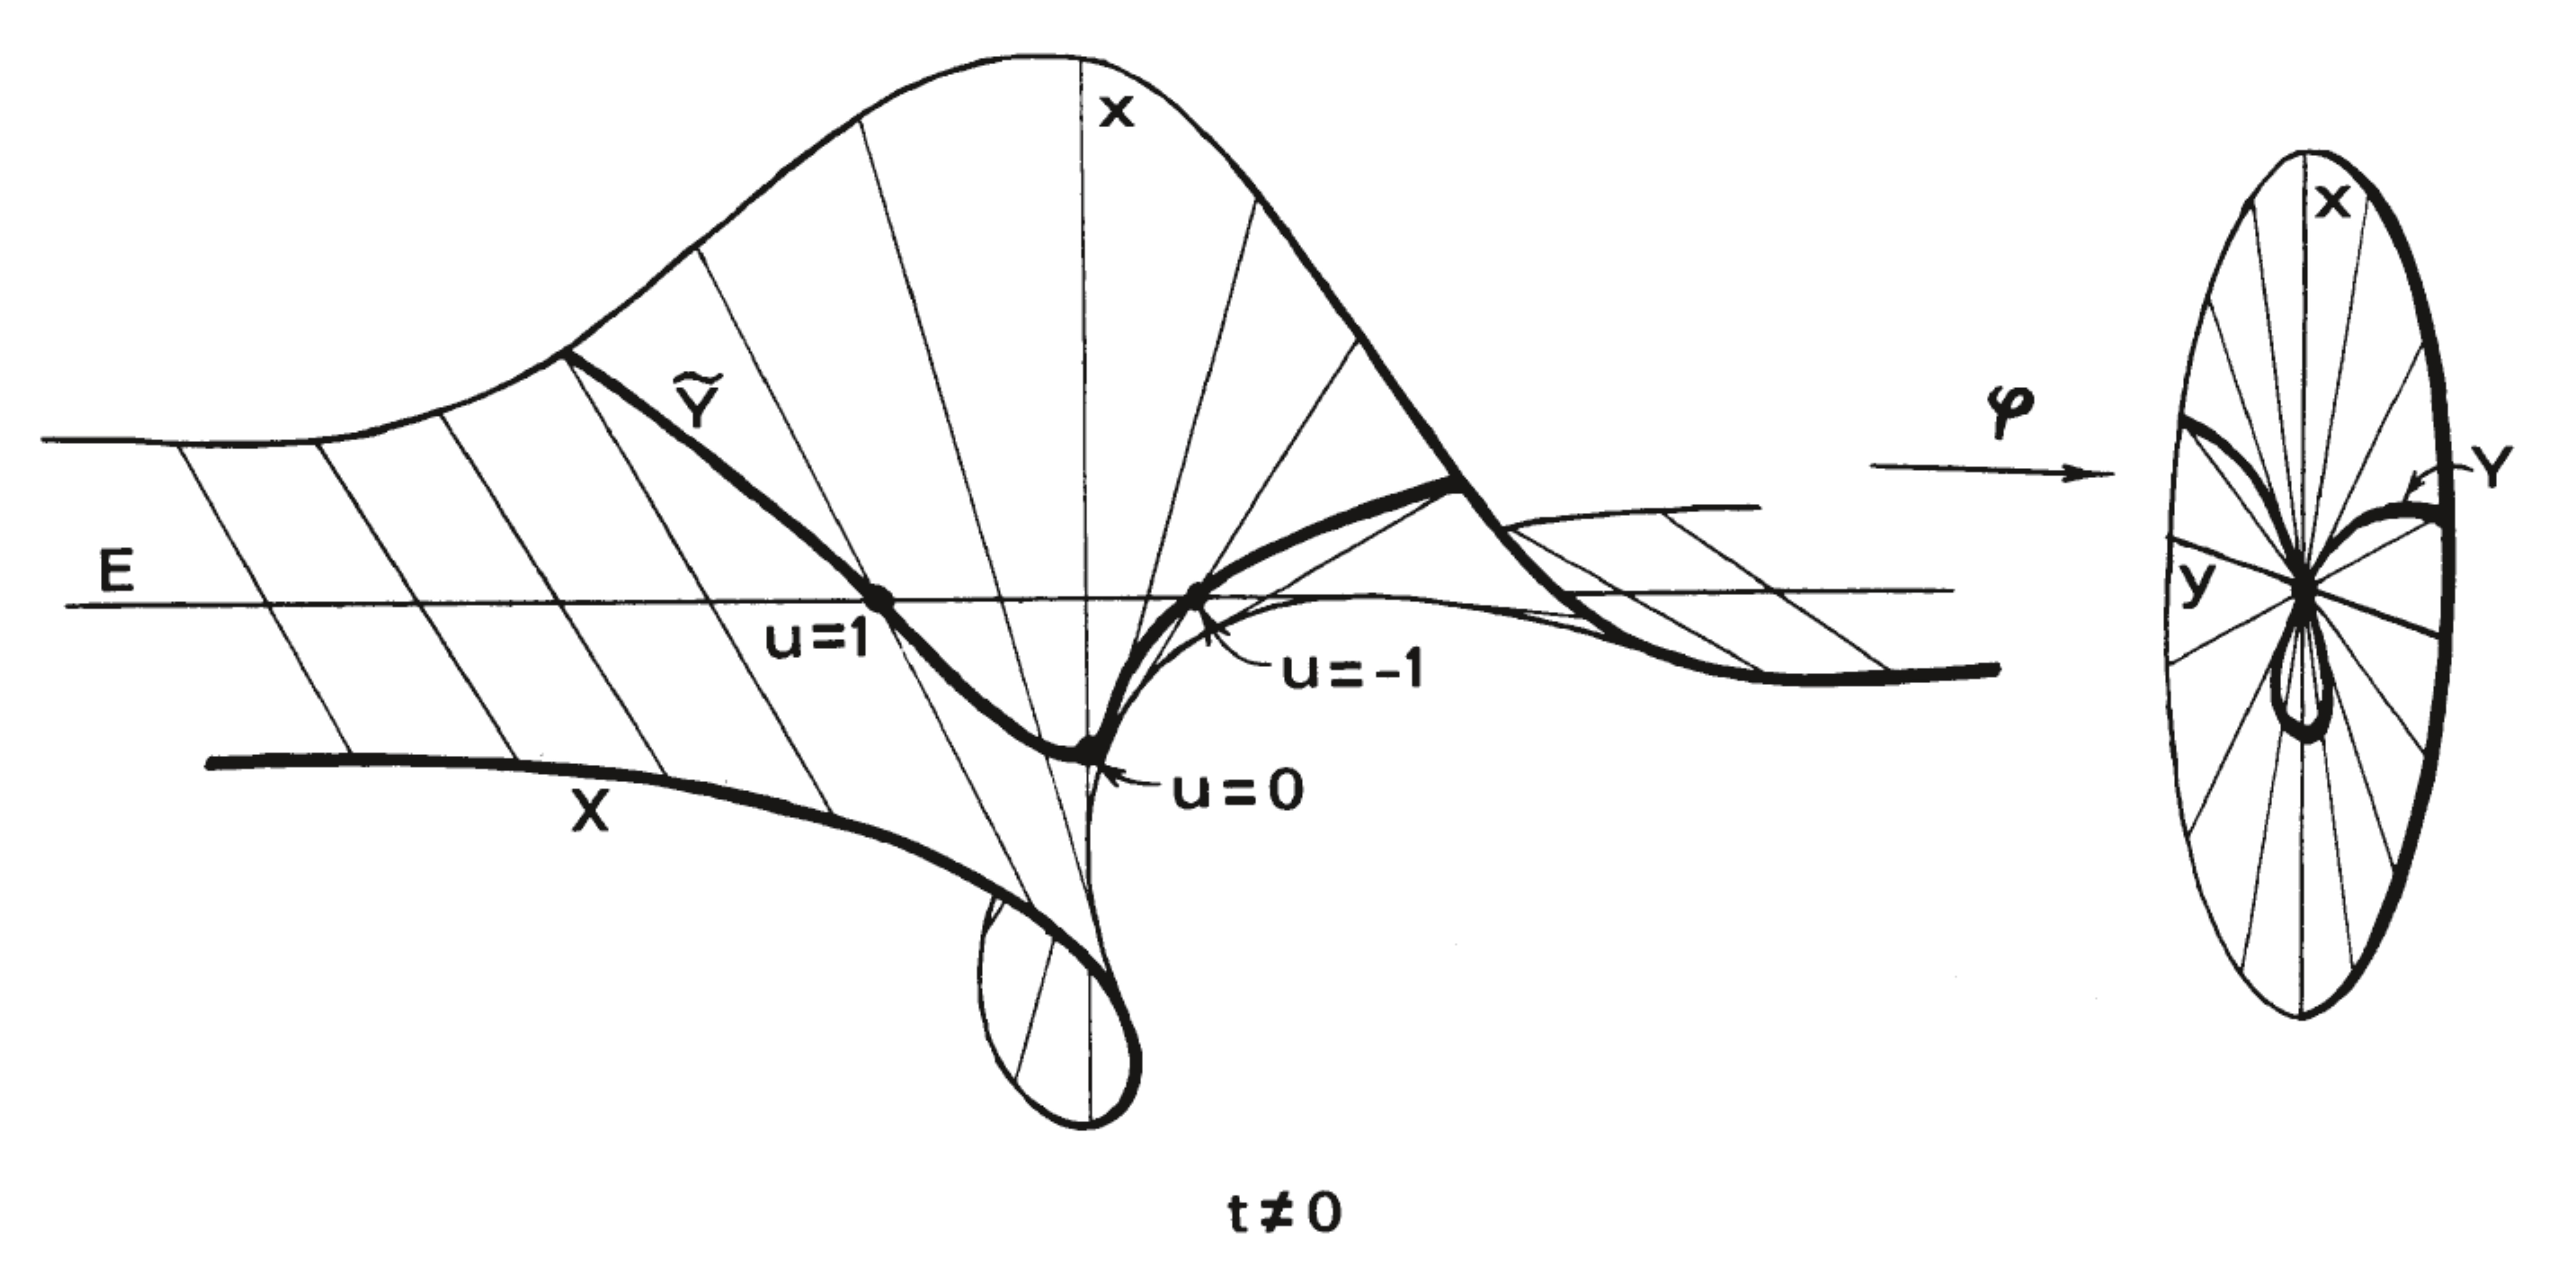
\includegraphics[width=0.8\columnwidth]{Figure3}\\
	Figure 3. 부풀림
	\end{center}
	
	
	%Definition
	\begin{definition}
	%
		\tn{$Y$가 $O$를 지나는 $\An$의 닫힌 부분대수다양체이면 \tb{$Y$의 점 $O$에서의 부풀림(blowing-up of $Y$ at the point $O$)}을
		$\tilde Y=\overline{(\ph^{-1}(Y-O))}$로 정의한다. 여기에서 $\ph:X\ra\An$은 위에 기술된 $\An$의 $O$에서의 부풀림이다.
		우리는 $\ph:X\ra\An$을 $\tilde Y$로 제한하여 얻어진 사상도 $\ph:\tilde Y\ta Y$로 표기한다.
		$\An$의 임의의 다른 점 $P$에서 부풀리기 위해서는 $P$를 $O$로 대응시키는 좌표계의 1차다항식에 의한 변환을 가하라.}
	%
	\end{definition}
	
	$\ph$가 $\tilde Y-\ph^{-1}(O)$와 $Y-O$ 간의 동형사상을 유도함을 기억해 두라.
	따라서 $\ph$는 $\tilde Y$에서 $Y$로의 쌍유리사상이다.
	또한 이러한 정의가 분명히 $Y$의 $\An$으로의 매장에 의존함을 기억해 두라.
	그러나 우리가 나중에 보일 것과 같이 사실 부풀림은 내재적이다. (II, 7.15.1)
	
	$Y$의 점에서의 부풀림의 효과는 $Y$를 $O$ 근처에서 $O$를 통과하는 다른 방향의 직선을 따라 `잡아 찢는' 것이다.
	우리는 이것을 예를 통해 소개하겠다.
	
	
	%Example 4.9.1
	\begin{example}
	%
		\tn{\\$Y$가 방정식 $y^2=x^2(x+1)$에 의해 주어진 평면 3차곡선이라 하자.
		우리는 $Y$를 $O$에서 부풀릴 것이다. (Fig. 3) $t,u$가 $\mb P^1$의 동차 좌표라 하자.
		그 경우 $\mb A^2$의 $O$에서의 부풀림 $X$는 $\mb A^2\times\mb P^1$ 내에서 방정식 $xu=ty$에 의해 정의된다.
		이는 점 $O$가 $O$를 통과하는 직선들의 기울기에 대응하는 $\mb P^1$로 대체된 것을 제외하면 $\mb A^2$처럼 보인다.
		우리는 이러한 $\mb P^1$을 \tb{예외곡선(exceptional curve)}이라 부르며 $E$로 표기할 것이다.\\
		우리는 $\mb A^2\times\mb P^1$에서 방정식 $y^2=x^2(x+1)$과 $xu=ty$를 고려하는 것으로 $Y$의 $X$에서의 전체 역상을 얻을 것이다.
		이제 $\mb P^1$은 열린집합 $t\ne 0$과 $u\ne 0$에 의해 덮이며 우리는 이들을 개별적으로 고려할 것이다.
		만약 $t\ne 0$이면 $t=1$이라 설정하고 $u$를 아핀 매개변수로 사용한다.
		그 경우 우리는 좌표계 $x,y,u$를 가지는 $\mb A^3$에서 다음 방정식을 얻는다.}
	%
		\begin{align*}
		y^2&=x^2(x+1)\\y&=xu
		\end{align*}
	%
		\tn{대입하면 우리는 $x^2u^2-x^2(x+1)=0$을 얻으며 이는 인수분해된다.
		그러므로 우리는 $x=0,y=0,$ 임의의 $u$에 의해 정의된 $E$와 $u^2=x+1,y=xu$에 의해 정의된 $\tilde Y$라는
		두 개의 기약 성분을 얻는다. $\tilde Y$가 $E$와 점 $u=\pm 1$에서 만남을 기억해 두라.
		이 점들은 $Y$의 $O$에서의 두 갈래의 기울기에 대응한다.\\
		마찬가지로 우리는 $x$축의 전체 역상이 $E$와 하나의 다른 기약 곡선으로 구성됨을 확인할 수 있으며
		우리는 이를 $x$축의 \tb{엄격한 변환(strict transform)}이라 한다.
		(이는 직선 $L=x$축에 대응하는 앞에서 기술한 곡선 $\bar L'$이다.)
		이러한 엄격한 변환은 점 $u=0$에서 $E$와 만난다. $\mb A^2\times\mb P^1$에서의 다른 열린집합 $u\ne 0$을 고려하면
		$y$축의 엄격한 변환이 $E$와 점 $t=0,u=1$에서 만남을 보일 수 있다.\\
		이러한 결론은 Figure 3에 요약되어 있다. 부풀림의 효과는 $O$를 통과하는 곡선의 가지들을 기울기에 따라 분리하는 것이다.
		만약 기울기가 다르다면 이들의 엄격한 변환은 $X$에서 만나지 않는다.
		대신 이들은 $E$와 서로 다른 기울기에 대응하는 점에서 만난다.}
	%
	\end{example}
	
	
	
	%Exercises
	\subsection*{Exercises (연습문제)}
	
	\begin{enumerate}[label=\tb{4.\arabic*.},itemindent=0mm,itemsep=2mm]
	\item 만약 $f$와 $g$가 대수다양체 $X$의 열린집합 $U$와 $V$ 상에서의 정칙 함수이며 $U\cap V$ 상에서 $f=g$이면
	$U$ 상에서 $f$이고 $V$ 상에서 $g$인 함수는 $U\cup V$ 상에서의 정칙 함수임을 보여라.
	만약 $f$가 $X$ 상에서의 \ti{유리}함수이면 $f$가 정칙 함수로 표현될 수 있도록 하는 $X$의 최대 열린 부분집합 $U$가 존재함을 보여라.
	우리는 $f$가 $U$의 점들에서 \tb{정의되었다(defined)}고 한다.
	\item 유리사상에 대한 동일한 문제. 만약 $\ph$가 $X$에서 $Y$로의 유리사상이면 $\ph$가 사상에 의해 표현되도록 하는
	최대 열린집합이 존재함을 보여라. 우리는 유리사상이 이러한 열린집합의 점들에서 \tb{정의되었다(defined)}고 한다.
	\item \begin{enumerate}[label=(\alph*)]
	\item $f$가 $f=x_1/x_0$에 의해 주어진 $\mb P^2$ 상에서의 유리함수라 하자.
	$f$가 정의된 점들의 집합을 찾고 대응하는 정칙 함수를 기술하라.
	\item 이제 이 함수를 $\mb P^2$에서 $\mb A^1$로의 유리사상으로 간주하자. $\mb A^1$을 $\mb P^1$에 매장하고
	$\ph:\mb P^2\ra\mb P^1$이 그 결과로 얻어진 유리사상이라 하자. $\ph$가 정의된 점들의 집합을 찾고 대응하는 사상을 기술하라.
	\end{enumerate}
	\item 대수다양체 $Y$가 \tb{유리(rational)}라는 것을 어떠한 $n$에 대하여 $\Pn$과 쌍유리동치인 것으로 정의하자.
	(또는 (4.5)에 의해 이와 동치로 $K(Y)$가 $k$의 순수히 초월적 확대인 것이다.)
	\begin{enumerate}[label=(\alph*)]
	\item $\mb P^2$에서의 임의의 원뿔곡선은 유리 곡선이다.
	\item 첨점을 가진 3차곡선 $y^2=x^3$은 유리 곡선이다.
	\item $Y$가 $\mb P^2$에서의 결절점을 가진 3차곡선 $y^2z=x^2(x+z)$라 하자. 점 $P=(0,0,1)$에서 직선 $z=0$으로의 사영 $\ph$%
	(Ex. 3.14)는 $Y$에서 $\mb P^1$으로의 쌍유리사상을 유도함을 보여라. 그러므로 $Y$는 유리 곡선이다.
	\end{enumerate}
	\item $\mb P^3$에서의 2차곡면 $Q:xy=zw$가 $\mb P^2$와 쌍유리이지만 $\mb P^2$와 동형은 아님을 보여라. (cf. Ex. 2.15)
	\item \tb{평면 Cremona 변환.} $\mb P^2$에서 자신으로의 쌍유리사상은
	\tb{평면 Cremona 변환(plane Cremona transformation)}이라 불린다.
	\tb{2차 변환(quadratic transformation)}이라 불리는 예를 제시하겠다. 이는 $a_0,a_1,a_2$ 중 두 개가 0이지는 않은 경우
	$(a_0,a_1,a_2)\ra(a_1a_2,a_0a_2,a_0a_1)$에 의해 주어진 유리사상 $\ph:\mb P^2\ra\mb P^2$이다.
	\begin{enumerate}[label=(\alph*)]
	\item $\ph$가 쌍유리이며 스스로의 역임을 보여라.
	\item $\ph:U\ra V$가 동형사상이도록 하는 열린집합 $U,V\bseq\mb P^2$를 찾아라.
	\item $\ph$와 $\ph^{-1}$이 정의된 열린집합을 찾고 대응되는 사상을 기술하라. (V, 4.2.3)도 참조하라.
	\end{enumerate}
	\item $X$와 $Y$가 대수다양체라 하자. 점 $P\in X$와 $Q\in Y$가 존재하여
	국소환 $\mc O_{P,X}$와 $\mc O_{Q,Y}$가 $k$-대수로서 동형이라 하자.
	그 경우 열린집합 $P\in U\bseq X$와 $Q\in V\bseq Y$와 $P$를 $Q$로 대응시키는 $U$에서 $V$로의 동형사상이 존재한다.
	\item \begin{enumerate}[label=(\alph*)]
	\item $k$ 상에서의 임의의 양수 차원 대수다양체가 $k$와 동일한 기수를 가짐을 보여라.
	[Hint: 먼저 $\An$과 $\Pn$에 대하여 보여라. 그 후 임의의 $X$에 대하여 차원 $n$에 대한 귀납법을 사용하라.
	(4.9)를 사용하여 $X$가 초곡면 $H\bseq\mb P^{n+1}$과 쌍유리이도록 하라. (Ex. 3.7)을 사용하여
	$H$에 속하지 않은 한 점에서 $\Pn$으로의 $H$의 사영이 유한 개 점을 한 점으로 대응시키며 전사임을 보여라.]
	\item $k$ 상에서의 임의의 두 \ti{곡선}이 위상동형임을 연역하라. (cf. Ex. 3.1)
	\end{enumerate}
	\item $X$가 $\Pn$에서의 $r$차원 사영 대수다양체이며 $n\ge r+2$라 하자.
	적절한 $P\notin X$와 선형 대수다양체 $\mb P^{n-1}\bs\Pn$의 선택에 대하여 $P$에서 $\mb P^{n-1}$로의 사영(Ex. 3.14)이
	$X$에서 그 상 $X'\bseq\mb P^{n-1}$으로의 \ti{쌍유리사상}인 사상을 유도함을 보여라.
	(4.6A), (4.7A), (4.8A)가 필요할 것이다. 이는 특히 (4.9)의 쌍유리사상이 이러한 유한 번의 사영을 통해 얻어질 수 있음을 보여준다.
	\item $Y$가 $\mb A^2$에서의 첨점을 가진 3차곡선 $y^2=x^3$이라 하자.
	점 $O=(0,0)$을 부풀리고 $E$가 예외곡선이며 $\tilde Y$가 $Y$의 엄격한 변환이라 하자.
	$E$가 $\tilde Y$와 한 점에서 만나며 $\tilde Y\cong\mb A^1$임을 보여라.
	이 경우 사상 $\ph:\tilde Y\ra Y$가 전단사 쌍연속이지만 동형사상은 아니다.
	\end{enumerate}
	
	
	
	%Section 5
	\section{Nonsingular Varieties (비특이 대수다양체)}
	%
	대수기하학에서 비특이 대수다양체의 개념은 위상수학에서 다양체의 개념에 대응된다.
	예를 들어 복소수체 상에서 비특이 대수다양체들은 `표준'위상이 복소다양체인 것들이다.
	그러므로 가장 자연스러운 (그리고 역사적으로 먼저 등장했던) 비특이성의 정의는
	대수다양체를 정의하는 함수들의 도함수를 이용하는 것이다:
	
	
	%Definition
	\begin{definition}
	%
		\tn{$Y\bseq\An$이 아핀 대수다양체이며 $f_1,\ldots,f_t\in A=k[x_1,\ldots,x_n]$이 $Y$의 아이디얼의 생성집합이라 하자.
		$Y$가 \tb{점 $P\in Y$에서 비특이(nonsingular at a point $P\in Y$)}임은
		행렬 $\|(\pa f_i/\pa x_j)(P)\|$의 계수가 $n-r$인 것이다. (여기에서 $r$은 $Y$의 차원이다.)
		$Y$가 \tb{비특이(nonsingular)}임은 모든 점에서 비특이인 것이다.}
	%
	\end{definition}
	
	몇 가지를 첨언하겠다. 먼저 다항식의 어떠한 한 변수에 대한 편도함수의 개념은 임의의 체 상에서 유효하다.
	(통상적인 미분 규칙을 적용하면 된다.) 그러므로 극한 과정이 필요하지 않다. 그러나 표수 $p>0$의 경우 웃긴 일이 발생할 수 있다.
	예를 들어 $f(x)=x^p$이면 ($k$에서 $p=0$이므로) $df/dx=px^{p-1}=0$이다.
	모든 경우 만약 $f\in A$가 다항식이면 각각의 $i$에 대하여 $\pa f/\pa x_i$는 다항식이다.
	행렬 $\|(\pa f_i/\pa x_j)(P)\|$는 $P$에서의 \tb{Jacobi 행렬(Jacobian matrix)}이라 불린다.
	이러한 비특이성의 정의가 $Y$의 아이디얼의 생성집합의 선택에 독립적임을 간단히 보일 수 있다.
	
	우리의 정의의 한 가지 문제점은 $Y$의 아핀 공간으로의 매장에 의존한다는 것이다.
	그러나 기본적인 문헌 Zariski [1]에서 비특이성은 국소환에 의해 내재적으로 기술될 수 있음이 밝혀졌다.
	우리의 경우 그 결과는 다음과 같다.
	
	%Definition
	\begin{definition}
	%
		\tn{$A$가 Noether 국소환이며 극대 아이디얼 $\mf m$과 잉여류체 $k=A/\mf m$을 가진다 하자.
		$A$가 \tb{정칙 국소환(regular local ring)}이라는 것의 정의는 $\dim[k]\mf m/\mf m^2=\dim A$인 것이다.}
	%
	\end{definition}
	
	
	%Theorem 5.1
	\begin{theorem}
	%
		\tn{$Y\bseq\An$이 아핀 대수다양체라 하자. $P\in Y$가 점이라 하자.
		그 경우 $Y$가 $P$에서 비특이일 필요충분조건은 국소환 $\mc O_{P,Y}$가 정칙 국소환인 것이다.\\\\
	%
		\pf $P$가 $\An$에서의 점 $(a_1,\ldots,a_n)$이며 $\mf a_P=(x_1-a_1,\ldots,x_n-a_n)$이
		대응하는 $A=k[x_1,\ldots,x_n]$에서의 극대 아이디얼이라 하자.
		선형 사상 $\ta:A\ra k^n$을 임의의 $f\in A$에 대하여 다음과 같이 정의한다.}
	%
		$$\ta(f)=\Braket{\pdif f{x_1}(P),\ldots,\pdif f{x_n}(P)}$$
	%
		\tn{이제 $i=1,\ldots,n$에 대하여 $\ta(x_i-a_i)$들이 $k^n$의 기저를 형성하며 $\ta(\mf a_P^2)=0$임은 명백하다.
		그러므로 $\ta$는 동형사상 $\ta':\mf a_P/\mf a_P^2\ra k^n$을 유도한다.\\
		이제 $\mf b$가 $Y$의 $A$에서의 아이디얼이며 $f_1,\ldots,f_t$가 $\mf b$의 생성집합이라 하자.
		그 경우 Jacobi 행렬 $J=\|(\pa f_i/\pa x_j)(P)\|$의 계수는 $k^n$의 부분공간으로서 $\ta(\mf b)$의 차원이다.
		동형사상 $\ta'$을 이용하면 이는 $\mf a_P/\mf a_P^2$의 부분공간 $(\mf b+\mf a_P^2)/\mf a_P^2$의 차원과 동일하다.
		반면에 $Y$ 상에서의 $P$의 국소환 $\mc O_P$는 $A$를 $\mf b$로 나누고 극대 아이디얼 $\mf a_P$에서 국소화하여 얻어진다.
		그러므로 만약 $\mf m$이 $\mc O_P$의 극대 아이디얼이면 다음이 성립한다.}
	%
		$$\mf m/\mf m^2\cong\mf a_P/(\mf b+\mf a_P^2)$$
	%
		\tn{벡터 공간의 차원을 계산하면 $\dim\mf m/\mf m^2+\rank J=n$을 얻는다.\\
		이제 $\dim Y=t$이라 하자. 그 경우 $\mc O_P$는 $r$차원의 국소환이며 (3.2)
		따라서 $\mc O_P$가 정칙일 필요충분조건은 $\dim[k]\mf m/\mf m^2=r$인 것이다.
		그러나 이는 $\rank J=n-r$임과 동치이며 이는 $P$가 $Y$의 비특이점인 것과 동치이다.}
	%
	\end{theorem}
	
	\ti{Note}. 나중에 우리는 $Y$ 상에서의 미분 형식들의 층에 의한 비특이점의 다른 특성화를 제시할 것이다. (II, 8.15)\\
	
	이제 우리는 비특이성의 개념이 내재적임을 알게 되었으므로 정의를 임의의 대수다양체로 확장할 수 있다.
	
	
	%Definition
	\begin{definition}
	%
		\tn{$Y$가 임의의 대수다양체라 하자. $Y$가 점 $P\in Y$에서 \tb{비특이(nonsingular)}라는 것의 정의는
		국소환 $\mc O_{P,Y}$가 정칙 국소환인 것이다. $Y$가 \tb{비특이(nonsingular)}라는 것의 정의는 모든 점에서 비특이인 것이다.
		$Y$가 \tb{특이(singular)}라는 것의 정의는 비특이가 아닌 것이다.}
	%
	\end{definition}
	
	우리의 다음 목표는 대수다양체의 대부분의 점들이 비특이임을 보이는 것이다. 이를 위해서는 대수학적 예비지식이 필요하다.
	
	
	%Proposition 5.2A
	\begin{propositiona}
	%
		\tn{\\만약 $A$가 Noether 국소환이며 극대 아이디얼 $\mf m$과 잉여류체 $k$를 가지면
		$\dim[k]\mf m/\mf m^2\ge\dim A$이다.\\\\
	%
		\pf Atiyah-Macdonald [1, Cor. 11.15, p.121] 또는 Matsumura [2, p. 78]}
	%
	\end{propositiona}
	
	
	%Theorem 5.3
	\begin{theorem}
	%
		\tn{\\$Y$가 대수다양체라 하자. $Y$의 특이점들의 집합 $\Sing Y$는 $Y$의 닫힌 진부분집합이다.\\\\
	%
		\pf (II, 8.16을 참조하라.) 먼저 우리는 $\Sing Y$가 닫힌 부분집합임을 보일 것이다.
		$Y$의 어떠한 열린 덮개 $Y=\bigcup Y_i$에 대하여 각각의 $i$에 대하여 $\Sing Y_i$가 닫혀 있음을 보이면 충분하다.
		따라서 (4.3)에 의해 우리는 $Y$가 아핀이라 가정할 수 있다. (5.2)와 (5.1)의 증명에 의해
		우리는 Jacobi 행렬의 계수가 항상 $n-r$ 이하임을 알고 있다. 따라서 특이점들의 집합은 계수가 $n-r$ 미만인 곳이다.
		그러므로 $\Sing Y$는 $I(Y)$와 행렬 $\|\pa f_i/\pa x_j\|$의 모든 $(n-r)\times(n-r)$ 부분행렬들의 행렬식들에 의해
		생성된 아이디얼에 의해 정의된 대수적 집합이다. 따라서 $\Sing Y$는 닫혀 있다.\\
		$\Sing Y$가 $Y$의 진부분집합임을 보이기 위해 먼저 (4.9)를 적용하여 $Y$가 $\Pn$에서의 초곡면과 쌍유리임을 얻는다.
		쌍유리 대수다양체들은 동형인 열린집합들을 가지므로 초곡면의 경우로 문제를 줄일 수 있다.
		$Y$의 임의의 아핀 열린 부분집합을 고려하면 충분하며
		따라서 우리는 $Y$가 하나의 기약다항식 $f(x_1,\ldots,x_n)=0$에 의해 정의된 $\An$에서의 초곡면이라 가정할 것이다.\\
		이제 $\Sing Y$는 $i=1,\ldots,n$에 대하여 $(\pa f/\pa x_i)(P)=0$을 만족시키는 점 $P\in Y$들의 집합이다.
		만약 $\Sing Y=Y$이면 함수 $\pa f/\pa x_i$들이 $Y$ 상에서 항등적으로 0이며
		따라서 각각의 $i$에 대하여 $\pa f/\pa x_i\in I(Y)$이다. 그러나 $I(Y)$는 $f$에 의해 생성된 주 아이디얼이며
		각각의 $i$에 대하여 $\deg(\pa f/\pa x_i)\le\deg f-1$이므로 각각의 $i$에 대하여 $\pa f/\pa x_i=0$이어야 한다.\\
		표수 0의 경우 만약 $x_i$가 $f$에서 나타난다면 $\pa f/\pa x_i\ne 0$이므로 이는 불가능하다.
		따라서 $\Char k=p>0$이어야 한다. 이 경우 $\pa f/\pa x_i=0$이라는 사실은 $f$가 $x_i^p$의 다항식임을 함의한다.
		이는 각각의 $i$에 대하여 참이며 따라서 계수의 $p$제곱근을 취하면 ($k$가 대수적으로 닫혀 있으므로 이는 가능하다)
		$f=g^p$를 만족시키는 다항식 $g(x_1,\ldots,x_n)$을 얻는다. 그러나 이는 $f$가 기약이라는 전제조건에 모순이며
		따라서 $\Sing Y<Y$라 결론지을 수 있다.}
	%
		\qed
	%
	\end{theorem}
	
	
	
	%Subsection
	\subsection*{Completion (완비화)}
	%
	특이점을 국소적으로 분석하기 위해 우리는 이제 완비화의 기법을 기술할 것이다.
	$A$가 극대 아이디얼 $\mf m$을 가지는 국소환이라 하자.
	$\mf m$의 멱들은 $A$ 상에 \tb{$\mf m$진 위상($\mf m$-adic topology)}이라 불리는 위상을 정의한다.
	이러한 위상에 대하여 완비화하면 $\hat A$로 표기되는 $A$의 \tb{완비화(completion)}를 얻는다.
	이와 동치로 우리는 $\hat A$를 역극한 $\ds\lim_\longleftarrow A/\mf m^n$으로 정의할 수 있다.
	완비화에 관한 일반적인 정보를 위해서는
	Atiyah-Macdonald [1, Ch. 10], Matsumura [2, Ch. 9], 또는 Zariski-Samuel [1, Vol. 2, Ch. VIII]를 참조하라.
	
	완비화의 대수기하학에서의 중요성은 대수다양체 $X$ 상의 점 $P$에서의 국소환의 완비화 $\hO P$에서
	$X$의 $P$ 근처에서의 매우 국소적인 거동을 연구할 수 있다는 것이다.
	우리는 점 $P\in X$와 $Q\in Y$가 동형인 국소환을 가지면 $P$와 $Q$가 동형인 근방을 가지며 따라서 $X$와 $Y$가 쌍유리임을 보였다.
	(Ex. 4.7) 그러므로 통상적인 국소환 $\mc O_P$는 $X$의 거의 전체에 관한 정보를 포함한다.
	그러나 완비화 $\hO P$는 (앞으로 보게 될 것과 같이) 위상수학이나 미분기하학에서의 `국소'의 의미에 관한
	우리의 직관과 가까운 훨씬 더 국소적인 정보를 포함한다.
	
	우리는 완비화의 몇 가지 대수적 성질을 상기하고 예시를 제시하겠다.
	
	
	%Theorem 5.4A
	\begin{theorema}
	%
		\tn{\\$A$가 Noether 국소환이며 극대 아이디얼 $\mf m$을 가지고 $\hat A$가 그 완비화라 하자.
	%
		\begin{enumerate}[label=(\alph*)]
		\item $\hat A$는 극대 아이디얼 $\hat{\mf m}=\mf m\hat A$를 가지는 국소환이며
		자연스러운 단사 준동형사상 $A\ra\hat A$가 존재한다.
		\item 만약 $M$이 유한생성 $A$-모듈이면 그 $\mf m$진 위상에 대한 완비화 $\hat M$은 $M\otimes_A\hat A$와 동형이다.
		\item $\dim A=\dim\hat A$
		\item $A$가 정칙일 필요충분조건은 $\hat A$가 정칙인 것이다.
		\end{enumerate}}
	%
		\tn{\\\pf Atiyah-Macdonald [1, Ch. 10, 11] 또는 Zariski-Samuel [1, vol. 2, Ch. VIII]를 참조하라.}
	%
	\end{theorema}
	
	
	%Theorem 5.5A
	\begin{theorema}[Cohen Structure Theorem (Cohen 구조 정리)]
	%
		\tn{\\만약 $A$가 $n$차원 완비 정칙 국소환이며 어떠한 체를 포함하면
		$A\cong k[[x_1,\ldots,x_n]]$($A$의 잉여류체 $k$ 상에서의 형식적 멱급수환)이다.\\\\
	%
		\pf Matsumura [2, Cor. 2, p.206] 또는 Zariski-Samuel [1, vol. 2, Cor., p. 307]}
	%
	\end{theorema}
	
	
	%Definition
	\begin{definition}
	%
		\tn{두 점 $P\in X$와 $Q\in Y$가 \tb{해석적 동형(analayically isomorphic)}이라는 것의 정의는
		$k$-대수 동형사상 $\hO P\cong\hO Q$가 존재하는 것이다.}
	%
	\end{definition}
	
	
	\setcounter{theorem}{6}
	%Example 5.6.1
	\begin{example}
	%
		\tn{\\만약 $P\in X$와 $Q\in Y$가 해석적 동형이면 $\dim X=\dim Y$이다.
		이는 (5.4A)와 대수다양체 상의 임의의 점에서의 국소환은 대수다양체와 동일한 차원을 가진다는 사실에서 따라온다. (Ex. 3.12)}
	%
	\end{example}
	
	
	%Example 5.6.2
	\begin{example}
	%
		\tn{\\만약 $P\in X$와 $Q\in Y$가 같은 차원의 대수다양체 상의 비특이점들이면 $P$와 $Q$는 해석적 동형이다.
		이는 (5.4A)와 (5.5A)로부터 따라온다.
		이 예는 동일한 차원의 두 (위상, 미분, 복소)다양체가 국소적으로 동형이라는 사실의 대수적 유사체이다.}
	%
	\end{example}
	
	
	%Example 5.6.3
	\begin{example}
	%
		\tn{\\$X$가 방정식 $y^2=x^2(x+1)$에 의해 주어진 결절점을 가지는 평면 3차곡선이라 하자.
		$Y$가 $xy=0$에 의해 정의된 $\mb A^2$에서의 대수적 집합이라 하자.
		우리는 $X$ 상에서의 점 $O=(0,0)$이 $Y$ 상에서의 점 $O$와 대수적으로 동형임을 보일 것이다.
		(우리가 아직 기약 대수적 집합 상에서의 점의 국소환에 관한 일반적인 이론을 개발하지 않았으므로
		우리는 ad hoc 정의 $\mc O_{O,Y}=(k[x,y]/(xy))_{(x,y)}$를 사용할 것이다. 그러므로 $\hO{O,Y}\cong k[[x,y]]/(xy)$이다.)
		이러한 예는 $O$ 근처에서 $X$가 두 선이 교차하는 것처럼 보인다는 기하학적 사실에 대응된다.\\
		이 결과를 증명하기 위해 $k[[x,y]]/(y^2-x^2-x^3)$과 동형인 완비화 $\hO{O,X}$를 고려하자.
		핵심은 방정식의 주요 항 $y^2-x^2$가 서로 다른 두 인수 $y+x$와 $y-x$로 인수분해된다는 것이다.
		($\Char k\ne 2$라 가정한다.) $k[[x,y]]$에 속한 다음과 같은 두 형식적 멱급수가 존재하여 $g_i,h_i$가 동차 $i$차이며
		$y^2-x^2-x^3=gh$임을 주장하겠다.}
	%
		\begin{align*}
		g&=y+x+g_2+g_3+\cdots\\
		h&=y-x+h_2+h_3+\cdots
		\end{align*}
	%
		\tn{$g$와 $h$를 단계적으로 구축하겠다. $g_2$와 $h_2$를 결정하기 위해 다음이 필요하다.}
	%
		$$(y-x)g_2+(y+x)h_2=-x^3$$
	%
		\tn{$y-x$와 $y+x$가 $k[[x,y]]$의 극대 아이디얼을 생성하므로 이는 가능하다. $g_3$과 $h_3$을 결정하기 위해 다음이 필요하다.}
	%
		$$(y-x)g_3+(y+x)h_3=-g_2h_2$$
	%
		\tn{이는 다시 가능하며 이러한 방법으로 반복한다.\\
		그러므로 $\hO{O,X}=k[[x,y]]/(gh)$이다. $g$와 $h$가 선형 독립인 1차항으로 시작하므로 $k[[x,y]]$의 자기동형사상이 존재하여
		$g$와 $h$를 각각 $x$와 $y$로 대응시킨다. 이는 요구된 것과 같이 $\hO{O,X}\cong k[[x,y]]/(xy)$임을 보여준다.\\
		이 예에서 $\mc O_{O,X}$가 정역이지만 그 완비화는 정역이 아님을 기억해 두라.}
	%
	\end{example}
	
	아래의 (Ex. 5.15)에서 사용될 대수적 결과를 여기에 기술해 놓겠다.
	
	
	%Theorem 5.7A
	\begin{theorema}[Elimination Theory (소멸 이론)]
	%
		\tn{\\$f_1,\ldots,f_r$이 $x_0,\ldots,x_n$에 대한 동차다항식들이며 미정계수 $a_{ij}$들을 가진다 하자.
		그 경우 $a_{ij}$에 대한 정수계수 다항식들의 집합 $g_1,\ldots,g_t$가 존재하여
		각각의 $f_i$의 계수들에 대하여 개별적으로 동차이고 다음 성질을 가진다:
		임의의 체 $k$와 임의의 특정한 값 $a_{ij}\in k$들의 집합에 대하여
		$f_i$들이 $(0,\ldots,0)$ 이외의 공통영점을 가질 필요충분조건은 $a_{ij}$들이 다항식 $g_j$들의 공통영점인 것이다.\\\\
	%
		\pf Van der Waerden [1, Vol. II, \S 80, p. 8]}
	%
	\end{theorema}
	
	
	%Exercises
	\subsection*{Exercises (연습문제)}
	
	\begin{enumerate}[label=\tb{5.\arabic*.},itemindent=0mm,itemsep=2mm]
	\item $\mb A^2$에서의 다음 곡선들의 특이점의 위치를 찾고 형태를 그려라. ($\Char k\ne 2$라 가정하라.)
	각각의 방정식에 대응하는 곡선은 Figure 4에서 어떤 것인가?
	\begin{enumerate}[label=(\alph*)]
	\item $x^2=x^4+y^4$
	\item $xy=x^6+y^6$
	\item $x^3=y^2+x^4+y^4$
	\item $x^2y+xy^2=x^4+y^4$
	\end{enumerate}
	\end{enumerate}
	%
	%Figure 4
	\begin{center}
	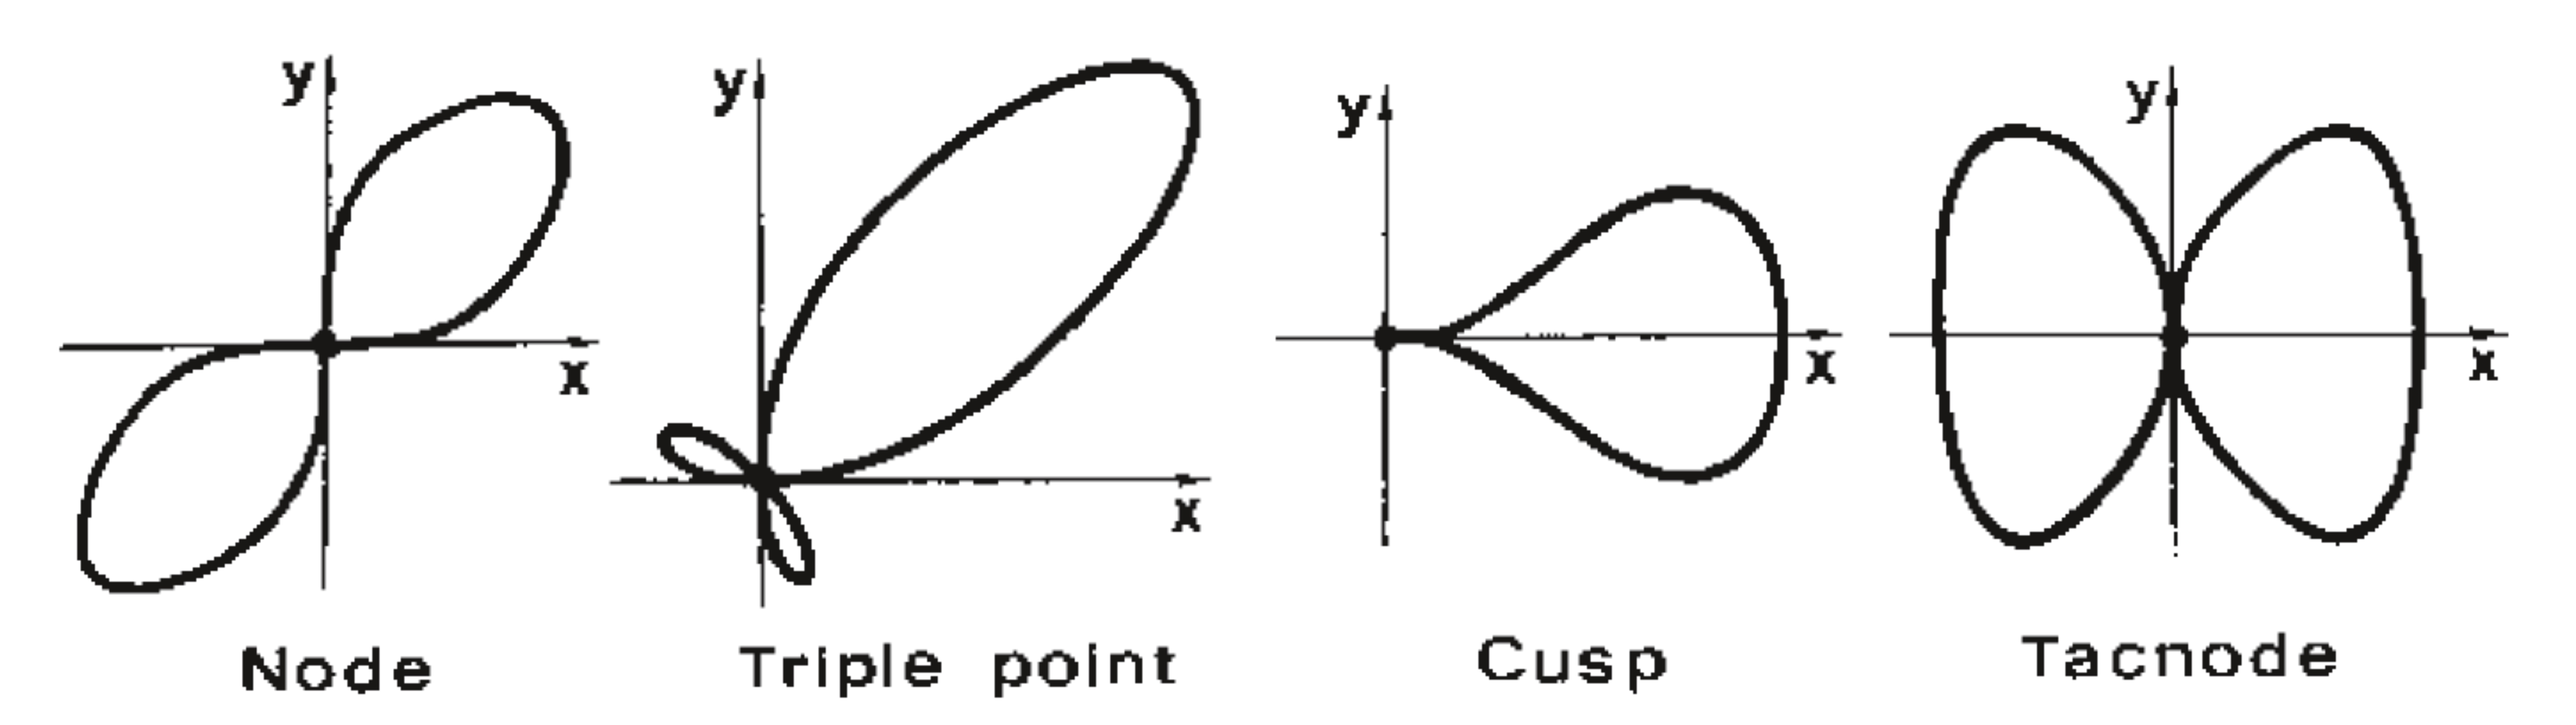
\includegraphics[width=0.8\columnwidth]{Figure4}\\
	Figure 4. 평면 곡선의 특이점
	\end{center}
	%
	\begin{enumerate}[label=\tb{5.\arabic*.},itemindent=0mm,itemsep=2mm]
	\setcounter{enumi}{1}
	\item 다음과 같은 $\mb A^3$에서의 곡면들의 특이점의 위치를 찾고 특이점을 기술하라. ($\Char k\ne 2$라 가정하라.)
	각각의 방정식에 대응하는 곡선은 Figure 5에서 어떤 것인가?
	\begin{enumerate}[label=(\alph*)]
	\item $xy^2=z^2$
	\item $x^2+y^2=z^2$
	\item $xy+x^3+y^3=0$
	\end{enumerate}
	\end{enumerate}
	%
	%Figure 5
	\begin{center}
	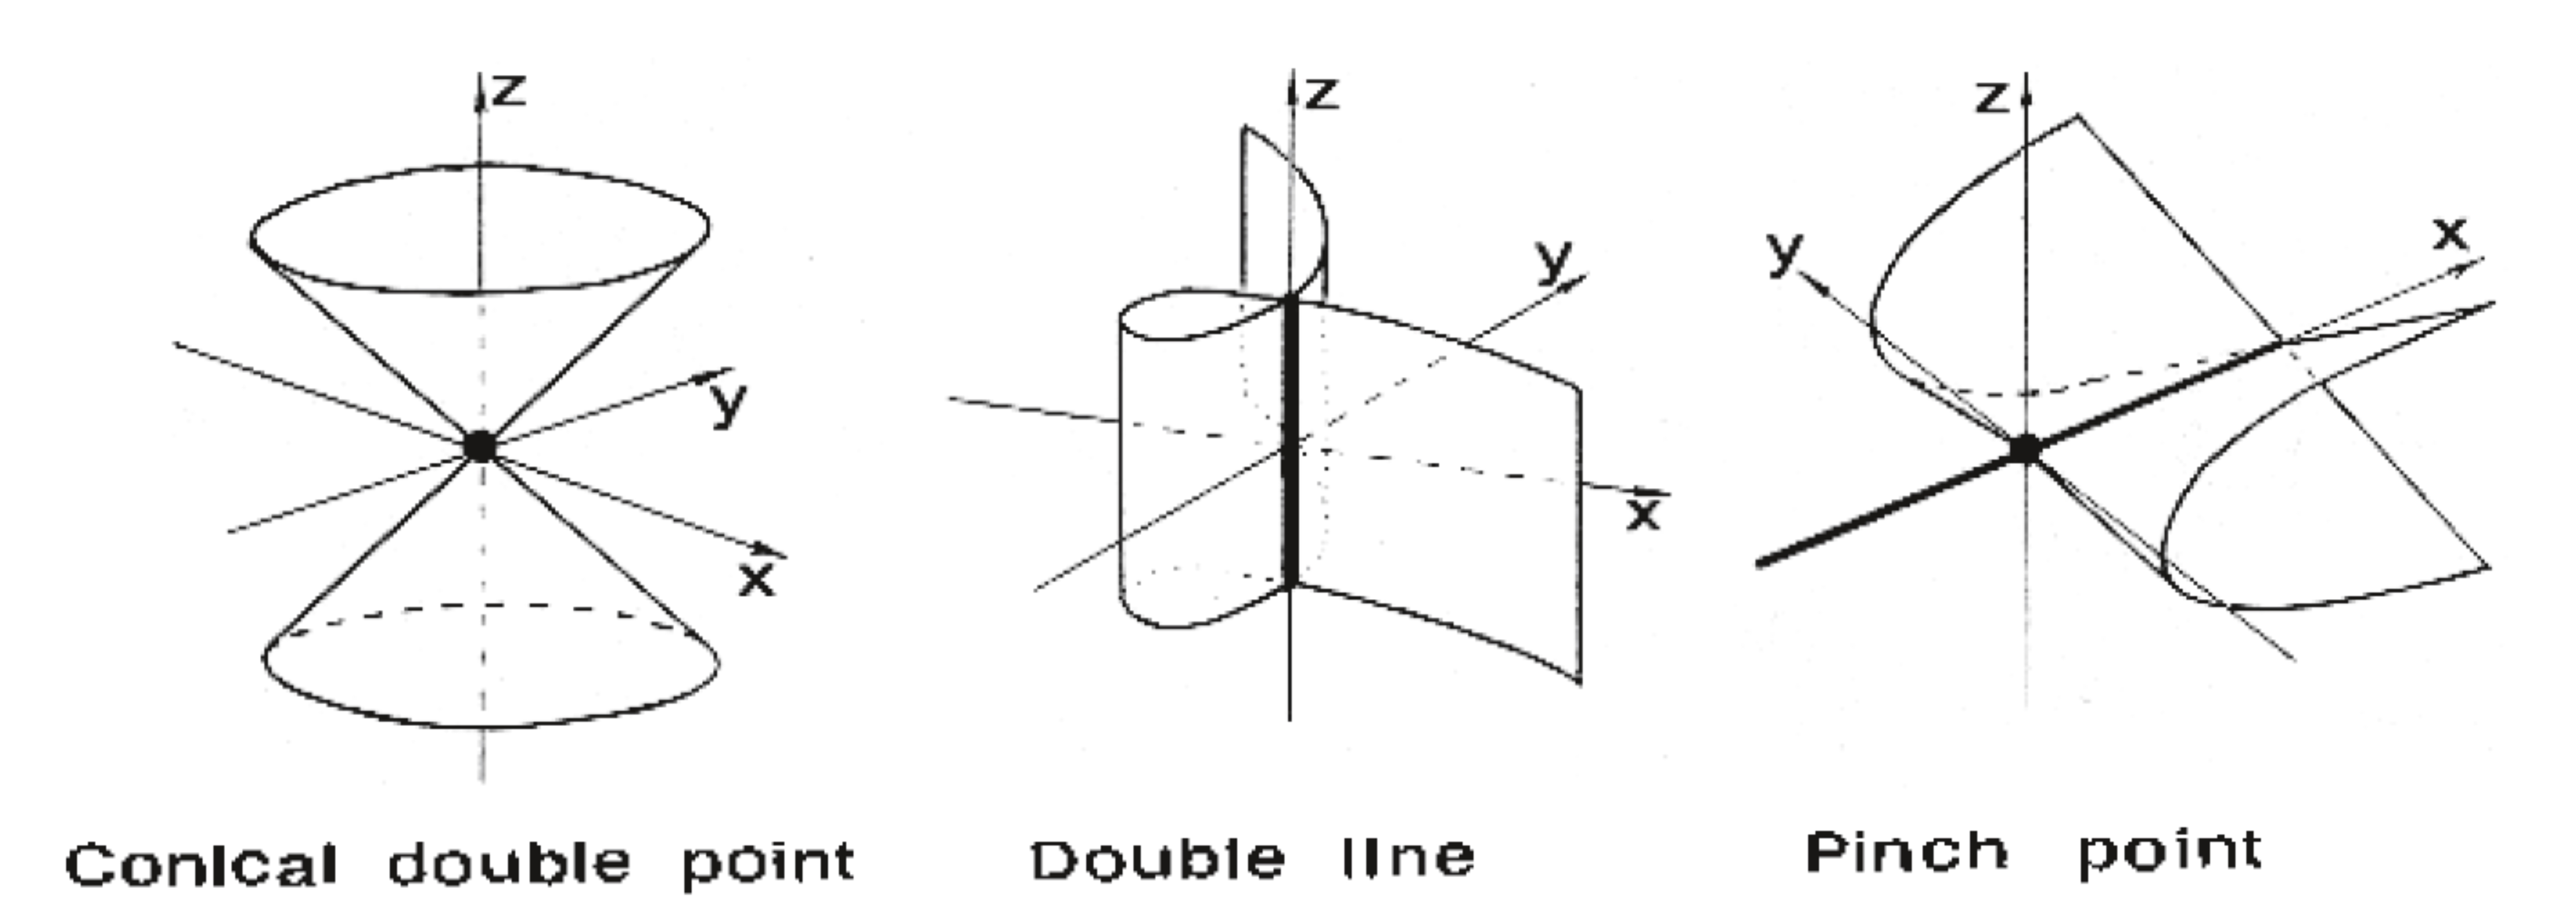
\includegraphics[width=0.8\columnwidth]{Figure5}\\
	Figure 5. 곡면 특이점
	\end{center}
	%
	\begin{enumerate}[label=\tb{5.\arabic*.},itemindent=0mm,itemsep=2mm]
	\setcounter{enumi}{2}
	\item \tb{중복도.} $Y\bseq\mb A^2$가 방정식 $f(x,y)=0$에 의해 정의된 곡선이라 하자. $P=(a,b)$가 $\mb A^2$의 점이라 하자.
	좌표계를 1차다항식에 의해 변환하여 $P$가 점 $(0,0)$이 되도록 하자.
	그 후 $f$를 $x$와 $y$에 대한 $i$차 동차다항식 $f_i$들의 합 $f=f_0+f_1+\cdots+f_d$로 표현하자.
	$P$의 $Y$ 상에서의 \tb{중복도(multiplicity)}를 $f_r\ne 0$이도록 하는 최소 $r$로 정의하고 $\mu_P(T)$로 표기하자.
	($P\in Y\Lra\mu_P(Y)>0$임을 기억해 두라.) $f_r$의 선형 인수들은 $P$에서의 \tb{접선방향(tangent direction)}들이라 불린다.
	\begin{enumerate}[label=(\alph*)]
	\item $\mu_P(T)=1\Lra P$가 $Y$의 비특이점인 것임을 보여라.
	\item 위의 (Ex. 5.1)에 있는 각각의 특이점들의 중복도를 찾아라.
	\end{enumerate}
	\item \tb{교차 중복도.} 만약 $Y,Z\bseq\mb A^2$가 서로 다른 두 곡선이며 방정식 $f=0,g=0$에 의해 주어지고 만약 $P\in Y\cap Z$이면
	$Y$와 $Z$의 $P$에서의 \tb{교차 중복도(intersection multiplicity)} $(Y\cdot Z)_P$를
	$\mc O_P$-모듈 $\mc O_P/(f,g)$의 길이로 정의한다.
	\begin{enumerate}[label=(\alph*)]
	\item $(Y\cdot Z)_P$가 유한하며 $(Y\cdot Z)_P\ge\mu_P(Y)\cdot\nu_P(Z)$임을 보여라.
	\item 만약 $P\in Y$이면 $P$를 통과하는 거의 모든(i.e. 유한 개를 제외한 모든) 직선 $L$에 대하여 $(L\cdot Y)_P=\mu_P(Y)$임을 보여라.
	\item 만약 $Y$가 $\mb P^2$에서의 $d$차곡선이며 $L$이 $\mb P^2$에서의 직선이고 $L\ne Y$이면 $(L\cdot Y)=d$임을 보여라.
	여기에서 $(L\cdot Y)=\sum(L\cdot Y)_P$(모든 점 $P\in L\cap Y$에 대한 합)로 정의하며
	$(L\cdot Y)_P$는 $\mb P^2$의 적절한 아핀 덮개를 이용하여 정의된다.
	\end{enumerate}
	\item 모든 차수 $d>0$과 $p=0$ 또는 임의의 소수 $p$에 대하여 표수 $p$의 체 $k$ 상에서의
	$\mb P^2$에서의 비특이 $d$차곡선의 방정식을 제시하라.
	\item \tb{곡선 특이점의 부풀림.}
	\begin{enumerate}[label=(\alph*)]
	\item $Y$가 (Ex. 5.1)의 첨점 또는 결절점을 가지는 곡선이라 하자. $Y$를 $O=(0,0)$에서 부풀려 얻어진 곡선 $\tilde Y$는 비특이이다.
	(cf. (4.9.1)과 (Ex. 4.10))
	\item \tb{결절점(node)}(또는 \tb{통상2중점(ordinary double point)})을 서로 다른 접선방향(Ex. 5.3)들을 가지는
	평면 곡선의 2중점(i.e. 중복도 2의 점)으로 정의한다.
	만약 $P$가 평면 곡선 $Y$ 상에서의 결절점이면 $\ph^{-1}(P)$가 부풀려진 곡선 $\tilde Y$ 상에서의
	서로 다른 두 개의 비특이점들로 구성됨을 보여라. 우리는 `$P$를 부풀리는 것이 $P$에서의 특이점을 해소한다'고 말한다.
	\item $P\in Y$가 (Ex. 5.1)의 접촉절점이라 하자.
	만약 $\ph:\tilde Y\ra Y$가 $P$에서의 부풀림이면 $\ph^{-1}(P)$가 ($\Char k\ne 2$인 경우) 결절점임을 보여라.
	(b)를 이용하면 우리는 접촉절점이 2회의 순차적인 부풀림에 의해 해소될 수 있음을 알 수 있다.
	\item $Y$가 평면 곡선 $y^3=x^5$라 하자. 이는 $O$에서 `고차 첨점'을 가진다.
	$O$가 3중점임을 보여라; $O$를 부풀리는 것은 2중점을 제공한다. (어떠한 형태의 2중점인가?) 한 번 더 부풀리면 특이점이 해소된다.
	\end{enumerate}
	\ti{Note}: 우리는 나중에 (V, 3.8) 평면 곡선의 임의의 특이점이 유한 회의 순차적인 부풀림에 의해 해소될 수 있음을 보일 것이다.
	\item $Y\bseq\mb P^2$가 방정식 $f(x,y,z)=0$에 의해 정의된 1차 초과의 비특이 평면 곡선이라 하자.
	$X\bseq\mb A^3$이 $f$에 의해 정의된 아핀 대수다양체라 하자. (이는 $Y$ 상에서의 뿔이다; (Ex. 2.10)을 참조하라.)
	$P$가 뿔의 \tb{꼭짓점(vertex)}인 점 $(0,0,0)$이라 하자. $\ph:\tilde X\ra X$가 $X$의 $P$에서의 부풀림이라 하자.
	\begin{enumerate}[label=(\alph*)]
	\item $X$가 하나의 특이점 $P$만을 가짐을 보여라.
	\item $\tilde X$가 비특이임을 보여라. (이를 아핀 열린집합들로 덮어라.)
	\item $\ph^{-1}(P)$가 $Y$와 동형임을 보여라.
	\end{enumerate}
	\item $Y\bseq\mb P^n$이 $r$차원 사영 대수다양체라 하자.
	$f_1,\ldots,f_t\in S=k[x_0,\ldots,x_n]$이 $Y$의 아이디얼을 생성하는 동차다항식들이라 하자.
	$P\in Y$가 동차 좌표 $P=(a_0,\ldots,a_n)$을 가지는 점이라 하자.
	$P$가 $Y$ 상에서 비특이일 필요충분조건은 행렬 $\|(\pa f_i/\pa x_j)(a_0,\ldots,a_n)\|$의 계수가 $n-r$인 것임을 보여라.
	[Hint: (a) 이러한 계수가 $P$에 대하여 선택된 동차 좌표계에 독립적임을 보여라.
	(b) $P$를 포함하는 아핀 열린집합 $U_i\bseq\Pn$으로 보내고 아핀 Jacobi 행렬을 사용하라.
	(c) $f$가 $d$차 동차이면 $\sum x_i(\pa f/\pa x_i)=d\cdot f$라는 Euler 보조정리가 필요할 것이다.]
	\item $f\in k[x,y,z]$가 동차다항식이고 $Y=Z(f)\bseq\mb P^2$가 $f$에 의해 정의된 대수적 집합이며
	모든 $P\in Y$에 대하여 $(\pa f/\pa x)(P),(\pa f/\pa y)(P),(\pa f/\pa z)(P)$ 중 적어도 하나가 0이라 하자.
	$f$가 기약(이며 따라서 $Y$가 비특이 대수다양체)임을 보여라. [Hint: (Ex 3.7)을 사용하라.]
	\item 대수다양체 $X$ 상에서의 점 $P$에 대하여 $\mf m$이 국소환 $\mc O_P$의 극대 아이디얼이라 하자.
	$X$의 $P$에서의 \tb{Zariski 접공간(Zariski tangent space)} $T_P(X)$를 $\mf m/\mf m^2$의 쌍대 $k$-벡터 공간으로 정의한다.
	\begin{enumerate}[label=(\alph*)]
	\item 임의의 점 $P\in X$에 대하여 $\dim T_P(X)\ge\dim X$이며 등호가 성립할 필요충분조건은 $P$가 비특이점인 것이다.
	\item 임의의 사상 $\ph:X\ra Y$에 대하여 자연스러운 유도 $k$-선형 사상 $T_P(\ph):T_P(X)\ra T_{\ph(P)}(Y)$가 존재한다.
	\item 만약 $\ph$가 포물선 $x=y^2$의 $x$축 상으로의 종방향 사영이면 원점에서의 접공간의 유도 사상 $T_0(\ph)$가 0 사상임을 보여라.
	\end{enumerate}
	\item \tb{$\mb P^3$에서의 타원 4차곡선.} $Y$가 방정식 $x^2-xz-yw=0$과 $yz-xw-zw=0$에 의해 정의된
	$\mb P^3$에서의 대수적 집합이라 하자. $P$가 점 $(x,y,z,w)=(0,0,0,1)$이며 $\ph$가 $P$에서 평면 $w=0$으로의 사영이라 하자.
	$\ph$가 $Y-P$와 평면 3차곡선 $y^2z-x^3+xz^2=0$에서 점 $(1,0,-1)$을 제외한 것 간의 동형사상을 유도함을 보여라.
	그 후 $Y$가 기약 비특이 곡선임을 보여라. 이는 $\mb P^3$에서의 \tb{타원 4차곡선(eliptic quartic curve)}이라 불린다.
	이것이 두 방정식에 의해 정의되었으므로 이는 완비 교집합의 또 다른 예시이다. (Ex. 2.17)
	\item \tb{2차초곡면.} $\Char k\ne 2$이며 $f$가 $x_0,\ldots,x_n$에 대한 2차 동차다항식이라 하자.
	\begin{enumerate}[label=(\alph*)]
	\item 좌표계를 적절한 1차다항식에 의해 변환하는 것으로 어떠한 $0\le r\le n$에 대하여
	$f$가 $f=x_0^2+\cdots+x_r^2=0$의 형태가 될 수 있음을 보여라.
	\item $f$가 기약일 필요충분조건은 $r\ge 2$인 것임을 보여라.
	\item $r\ge 2$라 가정하고 $Q$가 $f$에 의해 정의된 $\Pn$에서의 2차초곡면이라 하자.
	$Q$의 특이 자취 $Z=\Sing Q$가 $n-r-1$차원 \ti{선형} 대수다양체(Ex. 2.11)임을 보여라.
	특히 $Q$가 비특이일 필요충분조건은 $r=n$인 것이다.
	\item $r<n$인 경우 $Q$는 축이 $Z$인 비특이 2차초곡면 $Q'\bseq\mb P^r$ 상에서의 뿔임을 보여라.
	(이러한 뿔의 개념은 (Ex. 2.10)에서 정의된 것의 일반화이다. 만약 $Y$가 $\mb P^r$의 닫힌 부분집합이며
	$Z$가 $\Pn$에서의 $n-r-1$차원 선형 부분공간이면 $\mb P^r$을 $\Pn$에 매장하여 $\mb P^r\cap Z=\es$이도록 하고
	\tb{축이 $Z$인 $Y$ 상에서의 뿔(cone over $Y$ with axis $Z$)}를 $Y$의 점과 $Z$의 점을 통과하는 모든 직선들의 합집합으로 정의한다.)
	\end{enumerate}
	\item 모든 정칙 국소환은 정수적으로 닫힌 정역이다. (Matsumura [2, Th. 36, p. 121])
	그러므로 (5.3)에 의해 임의의 대수다양체는 정규점들의 공집합이 아닌 열린 부분집합을 가짐을 알 수 있다. (Ex. 3.17)
	이 연습문제에서 ((5.3)을 사용하지 않고) 대수다양체의 비정규점들의 집합이 닫힌 진부분집합임을 보여라.
	(정수적 폐포의 유한성이 필요할 것이다: (3.9A)를 참조하라.)
	\item \tb{해석적 동형 특이점.}
	\begin{enumerate}[label=(\alph*)]
	\item 만약 $P\in Y$와 $Q\in Z$가 해석적 동형 평면 곡선 특이점이면 중복도 $\mu_P(Y)$와 $\mu_Q(Z)$가 동일함을 보여라. (Ex. 5.3)
	\item 본문의 예시 (5.6.3)을 일반화하여 만약 $f=f_r+f_{r+1}+\cdots\in k[[x,y]]$이며
	$f$의 최고차 형식 $f_r$이 $f_r=g_sh_t$로 분해되고 $g_s,h_t$가 각각 $s$차와 $t$차 동차이며
	공통 1차 인수를 갖지 않으면 $k[[x,y]]$에서의 형식적 멱급수
	%
	\begin{align*}
	g&=g_s+g_{s+1}+\cdots\\h&=h_t+h_{t+1}+\cdots
	\end{align*}
	%
	가 존재하여 $f=gh$를 만족시킨다.
	\item $Y$가 $\mb A^2$에서 방정식 $f(x,y)=0$에 의해 정의되며 $P=(0,0)$이 $Y$ 상에서의 중복도 $r$인 점이고
	따라서 $f$가 $x$와 $y$에 대한 다항식으로 전개되었을 경우 $f=f_r+$고차항 형태이다.
	$P$가 \tb{통상$r$중점(ordinary $r$-fold point)}임을 $f_r$이 서로 다른 $r$개 선형 인수들의 곱인 것으로 정의한다.
	임의의 두 통상2중점이 해석적 동형임을 보여라. 통상3중점에 대해서도 위와 같다.
	그러나 서로 동형이 아닌 통상4중점들의 1매개변수족이 존재함을 보여라.
	\end{enumerate}
	\begin{enumerate}[label=*(\alph*)]
	\setcounter{enumii}{3}
	\item $\Char k\ne 2$라 가정하자. 평면곡선의 임의의 2중점들이 유일하게 결정된 $r\ge 2$에 대하여
	곡선 $y^2=x^r$의 $(0,0)$에서의 특이점과 해석적 동형임을 보여라.
	만약 $r=2$이면 이는 결절점이다. (Ex. 5.6) 만약 $r=3$이면 이는 \tb{첨점(cusp)}이다;
	만약 $r=4$이면 \tb{접촉절점(tacnode)}이다. 심화된 논의를 위해서는 (V, 3.9.5)를 참조하라.
	\end{enumerate}
	\item \tb{평면 곡선들의 족.} 3변수 $x,y,z$에 대한 $d$차 동차다항식 $f$는 $\binom{d+2}2$개 계수들을 가진다.
	이러한 계수들이 $N=\binom{d+2}2-1=\fra 2d(d+3)$인 $\mb P^N$에서의 점을 표현한다 하자.
	\begin{enumerate}[label=(\alph*)]
	\item 이것이 $\mb P^N$의 점들과 $d$차방정식에 의해 정의될 수 있는 $\mb P^2$의 대수적 집합들 간의 대응 관계를 제공함을 보여라.
	$f$가 다수의 인자를 가지는 몇 가지 경우를 제외하면 이러한 대응이 일대일임을 보여라.
	\item 이러한 대응 하에서 (기약) 비특이 $d$차곡선들이 $\mb P^N$의 공집합이 아닌 Zariski-열린 부분집합의 점들에
	일대일 대응됨을 보여라. [Hint: (1) 동차다항식 $\pa f/\pa x_0,\ldots,\pa f/\pa x_n$에 적용된 소멸 이론 (5.7A)를 사용하라.
	(2) 위의 (Ex. 5.5, 5.8, 5.9)를 사용하라.]
	\end{enumerate}
	\end{enumerate}
	
	
	
	%Section 6
	\section{Nonsingular Curves (비특이 곡선)}
	%
	대수다양체를 분류하는 문제를 고려하면서 우리는 비특이 사영 대수다양체가 가장 좋은 종류라는 발상에 기반하여
	여러 부분문제들을 구축할 수 있다: (a) 대수다양체를 쌍유리동치 하에서 분류하라;
	(b) 각각의 쌍유리동치류예서 비특이 사영 대수다양체를 찾아라; (c) 주어진 쌍유리동치류에 속한 비특이 사영 대수다양체들을 분류하라.
	
	일반적으로 세 문제는 모두 굉장히 어렵다. 그러나 곡선의 경우 상황이 훨씬 더 간단하다.
	이 절에서 우리는 각각의 쌍유리동치류에 유일한 비특이 사영 곡선이 존재함을 보여 문제 (b)와 (c)에 답할 것이다.
	또한 우리는 모든 곡선이 서로 쌍유리동치이지는 않음을 반례를 제시하여 보일 것이다. (Ex. 6.2)
	그러므로 $k$의 주어진 초월 차수 1의 유한생성 확대체 $K$에서%
	(우리는 이를 \tb{1차원 함수체(function field of dimension 1)}라 부를 것이다)
	우리는 $K$와 동일한 함수체를 가지는 \ti{유일한} 비특이 사영 곡선 $C_K$에 대하여 말할 수 있다.
	우리는 또한 $K_1,K_2$가 두 1차원 함수체이면 임의의 $k$-준동형사상 $K_2\ra K_1$은
	$C_{K_1}$에서 $C_{K_2}$로의 사상으로 표현될 수 있음을 보일 것이다.
	
	주어진 함수체에 대응된 `추상적 비특이 곡선'의 개념을 정의하는 것으로 우회적인 방법으로 우리의 연구를 시작하겠다.
	이것이 대수다양체임은 자명하지 않을 것이다. 그러나 우리는 다시 생각해보면 새롭게 정의하는 것이 없다는 사실을 알게 될 것이다.
	
	먼저 우리는 부치환과 Dedekind 정역에 대한 몇 가지 기본적인 사실들을 상기하겠다.
	
	
	%Definition
	\begin{definition}
	%
		\tn{$K$가 체이며 $G$가 전순서 가환군이라 하자. $G$에 속한 값을 가지는 $K$의 \tb{부치(valuation)}는
		모든 $x,y\in K,x,y\ne 0$에 대하여 다음을 만족시키는 함수 $v:K-\{0\}\ra G$이다.}
	%
		\begin{align*}
		(1)&\quad v(xy)=v(x)+v(y)\\(2)&\quad v(x+y)\ge\min(v(x),v(y))
		\end{align*}
	%
		\tn{만약 $v$가 부치이면 집합 $R=\sx{x\in K}{v(x)\ge 0}\cup\{0\}$은 $K$의 부분환이며
		$v$의 \tb{부치환(valuation ring)}이라 불린다.
		부분집합 $\mf m=\sx{x\in K}{v(x)>0}\cup\{0\}$은 $R$에서의 아이디얼이며 $R_{\mf m}$은 국소환이다.
		\tb{부치환(valuation ring)}은 그 분수체의 어떠한 부치에 대한 부치환인 정역이다.
		만약 $R$이 부치환이며 분수체 $K$를 가지면 $R$이 \tb{$K$의 부치환(valuation ring of $K$)}이라 한다.
		만약 $k$가 모든 $x\in k-\{0\}$에 대하여 $v(x)=0$을 만족시키는 $K$의 부분체이면
		$v$가 \tb{$K/k$의 부치(valuation of $K/k$)}라 하며 $R$이 \tb{$K/k$의 부치환(valuation ring of $K/k$)}이라 한다.
		(부치환들이 일반적으로 Noether가 아님을 기억해 두라!)}
	%
	\end{definition}
	
	
	%Definition
	\begin{definition}
	%
		\tn{만약 $A,B$가 체 $K$에 포함된 국소환이면 $B$가 $A$를 \tb{지배한다(dominate)}는 것의 정의는
		$A\bs B$이며 $\mf m_B\cap A=\mf m_A$인 것이다.}
	%
	\end{definition}
	
	
	%Theorem 6.1A
	\begin{theorema}
	%
		\tn{\\$K$가 체라 하자. $K$에 포함된 국소환 $R$이 $K$의 부치환일 필요충분조건은
		$R$이 $K$에 포함된 국소환들의 집합의 지배 관계 하에서의 극대원인 것이다.
		$K$에 포함된 모든 국소환은 $K$의 어떠한 부치환에 의해 지배된다.\\\\
	%
		\pf Bourbaki [2, Ch. VI, \S 1, 3] 또는 Atiyah-Macdonald [1, Ch. 5, p. 65, 및 연습문제, p. 72]}
	%
	\end{theorema}
	
	
	%Definition
	\begin{definition}
	%
		\tn{부치 $v$가 \tb{이산(discrete)}이라는 것의 정의는 그 수치군 $G$가 정수군인 것이다.
		대응하는 부치환은 \tb{이산 부치환(discrete valuation ring)}이라 불린다.}
	%
	\end{definition}
	
	
	%Theorem 6.2A
	\begin{theorema}
	%
		\tn{\\$A$가 1차원 Noether 국소 정역이며 극대 아이디얼 $\mf m$을 가진다 하자. 그 경우 다음 조건들은 동치이다:\\[-2mm]
	%
		\begin{enumerate}[label=(\roman*)]
		\item $A$는 이산 부치환이다.
		\item $A$는 정수적으로 닫혀 있다.
		\item $A$는 정칙 국소환이다.
		\item $\mf m$이 주 아이디얼이다.
		\end{enumerate}}
	%
		\tn{\\\pf Atiyah-Macdonald [1, Prop. 9.2, p.94]}
	%
	\end{theorema}
	
	
	%Definition
	\begin{definition}
	%
		\tn{\tb{Dedekind 정역(Dedekind domain)}은 1차원 정수적으로 닫힌 Noether 정역이다.}
	%
	\end{definition}
	
	정수적으로 닫혀 있다는 것이 국소적 성질이므로 (Atiyah-Macdonald [1, Prop. 5.13, p. 63])
	Dedekind 정역의 비자명 소 아이디얼에서의 모든 국소화는 이산 부치환이다.
	
	
	%Theorem 6.3A
	\begin{theorema}
	%
		\tn{\\Dedekind 정역의 그 분수체의 유한 확대체 내에서의 정수적 폐포는 다시 Dedekind 정역이다.\\\\
	%
		\pf Zariski-Samuel [1, vol. 1, Th. 19, p. 281]}
	%
	\end{theorema}
	
	이제 우리는 $k$ 상에서 1차원인 함수체 $K$의 경우로 넘어가겠다. (여기에서 $k$는 고정된 대수적으로 닫힌 기반체이다.)
	우리는 함수체가 $K$인 비특이 곡선과 $K/k$의 이산 부치환들 간의 연결을 수립하고자 한다.
	만약 $P$가 비특이 곡선 $Y$ 상의 점이면 (5.1)에 의해 국소환 $\mc O_P$는 1차원 정칙 국소환이며
	따라서 (6.2A)에 의해 이는 이산 부치환이다. 그 분수체는 $Y$의 함수체 $K$이다.
	$k\bseq\mc O_P$이므로 $\mc O_P$는 $K/k$의 부치환이다.
	그러므로 $Y$의 국소환들은 $K/k$의 이산 부치환들의 집합 $C_K$의 부분집합을 정의한다.
	이는 아래의 추상적 비특이 곡선의 정의에 대한 동기를 부여한다. 그러나 먼저 몇 가지 선행지식이 필요하다.
	
	
	%Lemma 6.4
	\begin{lemma}
	%
		\tn{\\$Y$가 준사영 대수다양체이며 $P,Q\in Y$라 하고 $K(Y)$의 부분환으로서 $\mc O_Q\bs\mc O_P$라 하자. 그 경우 $P=Q$이다.\\\\
	%
		\pf 어떠한 $n$에 대하여 $Y$를 $\Pn$에 매장하자. $Y$를 그 폐포로 대체하면 우리는 $Y$가 사영이라 가정할 수 있다.
		좌표를 적절히 선형 변환하는 것으로 우리는 $P$와 $Q$가 $x_0=0$에 의해 정의된 초평면 $H_0$에 속하지 않는다 가정할 수 있다.
		그러므로 $P,Q\in Y\cap(\Pn-H_0)$이고 이는 아핀이므로 우리는 $Y$가 아핀 대수다양체라 가정할 수 있다.\\
		$A$가 $Y$의 아핀 좌표환이라 하자. 그 경우 극대 아이디얼 $\mf m,\mf n\bseq A$가 존재하여
		$\mc O_P=A_{\mf m}$과 $\mc O_Q=A_{\mf n}$을 만족시킨다. 따라서 $\mf m=\mf n$이며 그러므로 (3.2b)에 의해 $P=Q$이다.}
	%
	\end{lemma}
	
	
	%Lemma 6.5
	\begin{lemma}
	%
		\tn{\\$K$가 $k$ 상에서의 1차원 함수체이며 $x\in K$라 하자. 그 경우 $\sx{R\in C_K}{x\notin R}$은 유한집합이다.\\\\
	%
		\pf $R$이 부치환이면 $x\notin R$ iff $1/x\in\mf m_R$이다.
		따라서 $y=1/x$라 하면 우리는 $y\in K$이고 $y\ne 0$이면 $\sx{R\in C_K}{y\in\mf m_R}$이 유한집합임을 보여야 한다.
		만약 $y\in k$이면 이러한 $R$이 존재하지 않으므로 $y\notin k$라 가정하자.\\
		$y$에 의하여 생성된 $K$의 부분환 $k[y]$를 고려하자.
		$k$가 대수적으로 닫혀 있으므로 $y$는 $k$ 상에서 초월적이며 따라서 $k[y]$는 다항식환이다.
		이에 더해 $K$가 유한생성이며 $k$ 상에서 초월 차수 1이므로 $K$는 $k(y)$의 유한 확대체이다.
		이제 $B$가 $k[y]$의 $K$에서의 정수적 폐포라 하자. 그 경우 (6.3A)에 의해 $B$는 Dedekind 정역이다.
		또한 $B$는 유한생성 $k$-대수이다. (3.9A)\\
		이제 만약 $y$가 $K/k$의 이산 부치환 $R$에 포함된다면 $k[y]\bseq R$이며,
		$R$이 $K$에서 정수적으로 닫혀 있으므로 $B\bseq R$이다.
		$\mf n=\mf m_R\cap B$라 하자. 그 경우 $\mf n$은 $B$의 극대 아이디얼이며 $B$는 $R$에 의해 지배된다.
		그러나 $B_{\mf n}$도 $K/k$의 이산 부치환이므로 부치환의 극대성(6.1A)에 의해 $B_{\mf n}=R$이다.\\
		만약 이에 더해 $y\in\mf m_R$이면 $y\in\mf n$이다. 이제 $B$는 어떠한 아핀 대수다양체 $Y$의 아핀 좌표환이다. (1.4.6)
		$B$가 Dedekind 정역이므로 $Y$는 1차원이며 비특이이다.
		$y\in\mf n$임은 $y$가 $Y$ 상에서의 정칙 함수로서 $\mf n$에 대응하는 $Y$의 점 상에서 소멸함과 동치이다.
		그러나 $y\ne 0$이므로 이는 유한 개 점에서만 소멸할 수 있다;
		(3.2)에 의해 점들은 $B$의 극대 아이디얼과 일대일 대응되며 극대 아이디얼 $\mf n$에 의해 $R=B_{\mf n}$이 결정된다.
		따라서 우리는 요구된 것과 같이 유한 개 $R\in C_K$에 대해서만 $y\in\mf m_R$이라 결론지을 수 있다.}
	%
		\qed
	%
	\end{lemma}
	
	
	%Corollary 6.6
	\begin{corollary}
	%
		\tn{\\$K/k$의 임의의 이산 부치환은 어떠한 비특이 아핀 곡선 상에서의 점의 국소환과 동형이다.\\\\
	%
		\pf 주어진 $R$에 대하여 $y\in R-k$라 하자. (6.5)의 증명에서 사용된 구축은 이러한 곡선을 준다.}
	%
	\end{corollary}
	
	이제 우리는 추상적 비특이 곡선의 정의에 도달했다. $K$가 $k$ 상에서의 1차원 함수체(i.e. 초월 차수 1의 유한생성 확대체)라 하자.
	$C_K$가 $K/k$의 모든 이산 부치환들의 집합이라 하자. 우리는 $C_K$의 원소들을 때로는 \ti{점}이라 부를 것이며
	부치환 $R_P$를 $P\in C_K$로 표기할 것이다. 함수체 $K$를 가지는 임의의 비특이 곡선의 모든 국소환들이 $C_K$에 포함되므로
	(이러한 국소환들은 서로 다르며 (6.4) 따라서 무한히 많다. (Ex. 4.8)) $C_K$가 무한집합임을 기억해 두라.
	우리는 전체 공간과 유한 부분집합들을 닫힌집합으로 취하는 것으로 $C_K$를 위상공간으로 만들 수 있다.
	만약 $U\bseq C_K$가 $C_K$의 열린 부분집합이면 $U$ 상에서의 \tb{정칙 함수(regular function)}들의 환을
	$\mc O(U)=\bigcap_{P\in U}R_P$로 정의한다.
	원소 $f\in\mc O(U)$는 $f(P)$를 $f$의 $R_P$의 극대 아이디얼에서의 잉여류로 정의하는 것으로 $U$에서 $k$로의 함수 형식을 정의한다.
	((6.6)에 의해 임의의 $R\in C_K$에 대하여 $R$의 잉여류체가 $k$임을 기억해 두라.)
	만약 두 원소 $f,g\in\mc O(U)$가 동일한 함수를 정의한다면 무한히 많은 $P\in C_K$에 대하여 $f-g\in\mf m_P$이다.
	따라서 (6.5)와 그 증명에 의해 $f=g$이다.
	그러므로 우리는 $\mc O(U)$의 원소들을 $U$에서 $k$로의 함수들과 동일시할 수 있다.
	또한 (6.5)에 의해 임의의 $f\in K$는 어떠한 열린집합 $U$ 상에서의 정칙 함수임을 기억해 두라.
	그러므로 \S 3에서와 같이 정의된 $C_K$의 함수체는 단지 $K$이다.
	
	
	%Definition
	\begin{definition}
	%
		\tn{\tb{추상적 비특이 곡선(abstract nonsingular curve)}은 열린 부분집합 $U\bseq C_K$이다.
		여기에서 $K$는 $k$ 상에서의 1차원 함수체이고 유도된 위상을 가지며 그 열린 부분집합 상에서 정칙 함수의 유도된 개념을 가진다.}
	%
	\end{definition}
	
	이러한 추상적 곡선이 대수다양체임은 자명하지 않다. 따라서 우리는 추상적 곡선들을 추가하여 대수다양체의 범주를 확대할 것이다:
	
	
	%Definition
	\begin{definition}
	%
		\tn{추상적 비특이 곡선 또는 대수다양체 간의 \tb{사상(morphism)} $\ph:X\ra Y$는 모든 열린집합 $V\bseq Y$와
		모든 정칙 함수 $f:V\ra k$에 대하여 $f\circ\ph$가 $\ph^{-1}(V)$ 상에서의 정칙 함수이도록 하는 연속 함수이다.}
	%
	\end{definition}
	
	이제 우리는 명백히 범주를 확대하였으며
	모든 비특이 준사영 곡선이 추상적 비특이 곡선과 동형임을 보이며 그 역도 성립함을 보여야 한다.
	
	
	%Proposition 6.7
	\begin{proposition}
	%
		\tn{\\모든 비특이 준사영 곡선 $Y$는 추상적 비특이 곡선과 동형이다.\\\\
	%
		\pf $K$가 $Y$의 함수체라 하자. 그 경우 각각의 점 $P\in Y$의 국소환 $\mc O_P$는 (5.1)과 (6.2A)에 의해 $K/k$의 이산 부치환이다.
		이에 더해 (6.4)에 의해 서로 다른 점들은 $K$의 서로 다른 부분군들을 준다.
		따라서 $U\bseq C_K$가 $Y$의 국소환들의 집합이며 $\ph:Y\ra U$가 $\ph(P)=\mc O_P$에 의해 정의된 전단사 함수라 하자.\\
		먼저 우리는 $U$가 $C_K$의 열린 부분집합임을 보여야 한다.
		열린집합들이 유한집합의 여집합이므로 $U$가 공집합이 아닌 열린집합을 포함함을 보이면 충분하다.
		(4.3)에 의해 우리는 $Y$가 아핀이며 아핀 좌표환 $A$를 가진다 가정할 수 있다.
		그 경우 $A$는 유한생성 $k$-대수이며 (3.2)에 의해 $K$는 $A$의 분수체이고 $U$는 $A$의 극대 아이디얼에서의 국소화들의 집합이다.
		이러한 국소환들이 모두 이산 부치환들이므로 $U$는 사실 $A$를 포함하는 $K/k$의 모든 이산 부치환들로 구성된다.
		이제 $x_1,\ldots,x_n$이 $A$의 $k$ 상에서의 생성집합이라 하자. 그 경우 $A\bseq R_P$ iff $x_1,\ldots,x_n\in R_P$이다.
		그러므로 $U_i=\sx{P\in C_K}{x_i\in R_P}$라 하면 $U=\bigcap U_i$이다.
		그러나 (6.5)에 의해 $\sx{P\in C_K}{x_i\notin R_P}$는 유한집합이다.
		그러므로 각각의 $U_i$가 열린집합이며 따라서 $U$도 그러하다.\\
		그러므로 우리는 위에서 정의된 $U$가 추상적 비특이 곡선임을 보였다. $\ph$가 동형사상임을 보이기 위해
		우리는 임의의 열린집합 상에서의 정칙 함수들이 서로 같음을 확인하면 충분하다.
		그러나 이는 $U$ 상에서의 정칙 함수들의 정의와 임의의 열린집합 $V\bseq Y$에 대하여
		$\mc O(V)=\bigcap_{P\in V}\mc O_{P,Y}$라는 사실로부터 따라온다.}
	%
	\end{proposition}
	
	이제 우리는 곡선에서 사영 대수다양체로의 사상의 확장에 관한 결과가 필요하다. 이는 그 자체로도 흥미롭다.
	
	
	%Proposition 6.8
	\begin{proposition}
	%
		\tn{\\$X$가 추상적 비특이 곡선이며 $P\in X$이고 $Y$가 사영 대수다양체이며 $\ph:X-P\ra Y$가 사상이라 하자.
		그 경우 유일한 사상 $\bar\ph:X\ra Y$가 존재하여 $\ph$를 확장한다.\\\\
	%
		\pf 어떠한 $n$에 대하여 $Y$를 $\Pn$의 닫힌 부분집합으로서 매장하자.
		그 경우 $\ph$가 $X$에서 $\Pn$으로의 사상으로 확장됨을 보이면 충분하다;
		만약 그렇다면 그 상은 반드시 $Y$에 포함되어야 하기 때문이다. 그러므로 문제는 $Y=\Pn$인 경우로 줄어든다.\\
		$\Pn$이 동차 좌표계 $x_0,\ldots,x_n$을 가지며 $U$가 $x_0,\ldots,x_n$이 모두 0이 아닌 열린집합이라 하자.
		$n$에 대한 귀납법을 사용하여 우리는 $\ph(X-P)\cap U\ne\es$라 가정할 수 있다:
		만약 $\ph(X-P)\cap U=\es$이면 $\ph(X-P)\bseq\Pn-U$이다.
		그러나 $\Pn-U$는 $x_i=0$에 의해 정의된 초곡면 $H_i$들의 합집합이다.
		$\ph(X-P)$가 기약이므로 이는 어떠한 $i$에 대하여 $H_i$에 포함되어야 한다.
		이제 $H_i\cong\mb P^{n-1}$이므로 결과는 귀납법에 의해 따라와야 한다.
		그러므로 우리는 $\ph(X-P)\cap U\ne\es$라 가정할 것이다.\\
		각각의 $i,j$에 대하여 $x_i/x_j$는 $U$ 상에서의 정칙 함수이다.
		이를 $\ph$에 의해 당기는 것으로 $X$의 열린 부분집합 상에서의 정칙 함수 $f_{ij}$를 얻는다.
		이는 $X$ 상에서의 유리함수로 간주될 것이다. i.e. $K$가 $X$의 함수체인 경우 $f_{ij}\in K$이다.\\
		$v$가 부치환 $R_P$에 연관된 $K$의 부치라 하자. $r_i=v(f_{i0}),i=0,1,\ldots,n,r_i\in\Z$라 하자.
		그 경우 $x_i/x_j=(x_i/x_0)/(x_j/x_0)$이므로 다음이 성립한다.}
	%
		$$v(f_{ij})=r_i-r_j\qquad i,j=0,\ldots,n$$
	%
		\tn{$r_k$가 $r_0,\ldots,r_n$ 중 최소이도록 하는 $k$를 선택하자.
		그 경우 모든 $i$에 대하여 $v(f_{ik})\ge 0$이며 따라서 $f_{0k},\ldots,f_{nk}\in R_P$이다.
		이제 $\bar\ph(P)=(f_{0k}(P),\ldots,f_{nk}(P))$와 $Q\ne P$에 대하여 $\bar\ph(Q)=\ph(Q)$로 정의하자.
		$\bar\ph$가 $\ph$를 확장하는 $X$에서 $\Pn$으로의 유일한 사상임을 주장하겠다.
		유일성은 구축에 의해 명백하다. (또한 이는 (4.1)로부터 따라온다.)
		$\bar\ph$가 사상임을 보이기 위해서는 $\bar\ph(P)$의 근방에서의 정칙 함수들이
		$X$ 상에서의 정칙 함수들로 당겨짐을 보이면 충분하다. $U_k\bseq\Pn$이 $x_k\ne 0$인 열린집합이라 하자.
		그 경우 $f_{kk}(P)=1$이므로 $\bar\ph(P)\in U_k$이다. $U_k$는 아핀이며 아핀 좌표환이 다음과 같다.}
	%
		$$k[x_0/x_k,\ldots,x_n/x_k]$$
	%
		\tn{이러한 함수들은 구축에 의해 $P$에서 정칙인 $f_{0k},\ldots,f_{nk}$로 당겨진다.
		임의의 더 작은 근방 $\bar\ph(P)\in V\bseq U_k$에 대하여 $V$ 상에서의 정칙 함수들이
		$X$ 상에서의 정칙 함수들로 당겨짐이 따라온다. 따라서 $\bar\ph$는 사상이며 이는 증명을 완료한다.}
	%
	\end{proposition}
	
	이제 우리는 주요 결과에 도달했다.
	
	
	%Theorem 6.9
	\begin{theorem}
	%
		\tn{\\$K$가 $k$ 상에서의 1차원 함수체라 하자.
		그 경우 위에서 정의된 추상적 비특이 곡선 $C_K$는 비특이 사영 곡선과 동형이다.\\\\
	%
		\pf 증명의 발상은 다음과 같다: 우리는 먼저 $C=C_K$를 비특이 아핀 곡선들과 동형인 열린 부분집합 $U_i$들로 덮을 것이다.
		$Y_i$가 이러한 아핀 곡선의 사영 폐포라 하자. 그 후 우리는 (6.8)을 사용하여 사상 $\ph_i:C\ra Y_i$를 정의한다.
		다음으로 우리는 곱사상 $\ph:C\ra\prod Y_i$를 고려하고 $Y$가 $C$의 상의 폐포라 한다.
		그 경우 $Y$는 사영 곡선이며 우리는 $\ph$가 $C$에서 $Y$로의 동형사상임을 보일 것이다.\\
		먼저 $P\in C$가 임의의 점이라 하자. 그 경우 (6.6)에 의해 비특이 아핀 곡선 $V$와
		점 $Q\in V$가 존재하여 $R_P\cong\mc O_Q$를 만족시킨다.
		$V$의 함수체가 $K$임이 따라오며 그 경우 (6.7)에 의해 $V$는 $C$의 열린 부분집합과 동형이다.
		그러므로 우리는 모든 점 $P\in C$가 아핀 대수다양체와 동형인 열린 근방을 가짐을 보였다.\\
		$C$가 준컴팩트이므로 우리는 이를 아핀 대수다양체 $V_i$와 동형인 유한 개 열린 부분집합 $U_i$들로 덮을 수 있다.
		$V_i\bseq\mb A^{n_i}$로 매장하고 $\mb A^{n_i}$를 $\mb P^{n_i}$의 열린 부분집합으로 간주하며
		$Y_i$가 $V_i$의 $\mb P^{n_i}$에서의 폐포라 하자. 그 경우 $Y_i$는 사영 대수다양체이며
		$U_i$의 그 상으로의 동형사상인 사상 $\ph_i:U_i\ra Y_i$를 얻는다.\\
		(6.8)을 유한집합 $C-U_i$에 적용하면 $\ph_i$를 확장하는 사상 $\bar\ph_i:C\ra Y_i$를 얻는다.
		$\prod Y_i$가 사영 대수다양체 $Y_i$들의 곱이라 하자. (Ex. 3.16) 그 경우 $\prod Y_i$도 사영 대수다양체이다.
		$\ph:C\ra\prod Y_i$가 `대각' 함수 $\ph(P)=\prod\bar\ph_i(P)$라 하고 $Y$가 $\ph$의 상의 폐포라 하자.
		그 경우 $Y$는 사영 대수다양체이며 $\ph:C\ra Y$는 상이 $Y$에서 조밀한 사상이다. ($Y$가 곡선임이 따라온다.)\\
		이제 우리는 $\ph$가 동형사상임을 보여야 한다. 임의의 점 $P\in C$에 대하여 어떠한 $i$에 대하여 $P\in U_i$이다.
		우세 사상들의 다음과 같은 가환 도표가 존재한다:}
	%
		$$\begin{tikzcd}[column sep=large]U\arrow[r]\arrow[d,swap,"i"]&X\arrow[d,"f"]\\
		T\arrow[r]\arrow[ur,dashed]&Y\end{tikzcd}$$v
	%
		\tn{여기에서 $\pi$는 $i$번째 좌표로의 사영 함수이다. 그러므로 우리는 (Ex. 3.3)에 의해 국소환들의 포함 관계를 얻는다.}
	%
		$$\mc O_{\ph_i(P),Y_i}\hra\mc O_{\ph(P),Y}\hra\mc O_{P,C}$$
	%
		\tn{처음과 끝의 것은 동형이며 따라서 중간 것도 동형이다.
		그러므로 우리는 임의의 $P\in C$에 대하여 함수 $\ph_P^*:\mc O_{\ph(P),Y}\ra\mc O_{P,C}$는 동형사상이다.\\
		다음으로 $Q$가 $Y$의 임의의 점이라 하자. 그 경우 $\mc O_Q$는 $K/k$의 어떠한 이산 부치환 $R_P$에 의해 지배된다.
		(예를 들어 $\mc O_Q$의 정수적 폐포의 극대 아이디얼에서의 국소화.)
		그러나 어떠한 $P\in C$에 대하여 $R=R_P$이며 $\mc O_{\ph(P)}\cong R$이므로 (6.4)에 의해 $Q=\ph(P)$여야 한다.
		이는 $\ph$가 전사임을 보여준다. 그러나 $K$의 서로 다른 부분환들이 $C$의 서로 다른 점에 대응되므로 $\ph$는 명백히 단사이다.\\
		그러므로 $\ph$는 $C$에서 $Y$로의 전단사 사상이며 모든 $P\in C$에 대하여 $\ph_P^*$가 동형사상이므로
		(Ex. 3.3b)에 의해 $\ph$는 동형사상이다.}
	%
		\qed
	%
	\end{theorem}
	
	
	%Corollary 6.10
	\begin{corollary}
	%
		\tn{\\모든 추상적 비특이 곡선은 준사영 곡선과 동형이다.
		모든 비특이 준사영 곡선은 비특이 사영 곡선의 열린 부분집합과 동형이다.}
	%
	\end{corollary}
	
	
	%Corollary 6.11
	\begin{corollary}
	%
		\tn{\\모든 곡선은 비특이 사영 곡선과 쌍유리동치이다.\\\\
	%
		\pf 만약 $Y$가 임의의 곡선이며 함수체 $K$를 가지면 $Y$는 $C_K$와 쌍유리동치이며 이는 비특이 사영 곡선이다.}
	%
	\end{corollary}
	
	
	%Corollary 6.12
	\begin{corollary}
	%
		\tn{\\다음 세 범주는 동치이다:\\[-2mm]
	%
		\begin{enumerate}[label=(\roman*)]
		\item 비특이 사영 곡선과 우세 사상
		\item 준사영 곡선과 우세 유리사상
		\item $k$ 상에서의 1차원 함수체와 $k$-준동형사상
		\end{enumerate}}
	%
		\tn{\\\pf (i)에서 (ii)로의 자명한 함자가 존재한다.
		(ii)에서 (iii)으로의 함자 $Y\ra K(Y)$가 존재하며 이는 (4.4)에 의해 범주의 동치를 유도한다.
		순환을 완성시키기 위해서는 (iii)에서 (i)로의 함자를 찾아야 한다.\\
		함수체 $K$에 곡선 $C_K$를 대응시키자. (정리에 의해 이는 비특이 사영 곡선이다.)
		만약 $K_1\ra K_2$가 준동형사상이면 (ii) $\cong$ (iii)에 의해 이는 대응하는 곡선들의 유리사상를 유도한다.
		이는 열린집합 $U\bseq C_{K_1}$에서의 사상 $\ph:U\ra C_{K_2}$로 표현될 수 있다.
		(6.8)에 의해 $\ph$는 사상 $\bar\ph:C_{K_1}\ra C_{K_2}$로 확장된다.
		만약 $K_3\ra K_2\ra K_1$이 두 준동형사상이면 (6.8)의 유일성 부분에서
		대응하는 사상 $C_1\ra C_2\ra C_3$과 $C_1\ra C_3$이 호환됨이 따라온다. 따라서 $K\mt C_K$는 함자 (iii) $\ra$ (i)이다.
		이는 명백히 주어진 함자 (i) $\ra$ (ii) $\ra$ (iii)의 역이며 따라서 우리는 범주의 동치를 얻는다.}
	%
	\end{corollary}
	
	
	
	%Exercises
	\subsection*{Exercises (연습문제)}
	
	\begin{enumerate}[label=\tb{6.\arabic*.},itemindent=0mm,itemsep=2mm]
	\item \tb{유리(rational)} 곡선이 $\mb P^1$과 쌍유리동치인 곡선임을 상기하라. (Ex. 4.4)
	$Y$가 $\mb P^1$과 동형이 아닌 비특이 유리곡선이라 하자.
	\begin{enumerate}[label=(\alph*)]
	\item $Y$가 $\mb A^1$의 열린 부분집합과 동형임을 보여라.
	\item $Y$가 아핀임을 보여라.
	\item $A(Y)$가 유일 인수분해 정역임을 보여라.
	\end{enumerate}
	\item \tb{타원곡선.} $Y$가 $\mb A^2$에서의 곡선 $y^2=x^3-x$라 하고 기반체 $k$의 표수가 2가 아니라 하자.
	이 연습문제에서 우리는 $Y$가 유리 곡선이 아니며 따라서 $K(Y)$가 $k$의 순수히 초월적 확대가 아님을 보일 것이다.
	\begin{enumerate}[label=(\alph*)]
	\item $Y$가 비특이임을 보이고 $A=A(Y)\cong k[x,y]/(y^2-x^3+x)$가 정수적으로 닫힌 정역임을 연역하라.
	\item $k[x]$가 $x$의 $A$에서의 상에 의해 생성된 $K=K(Y)$의 부분환이라 하자.
	$k[x]$가 다항식환이며 $A$가 $k[x]$의 $K$에서의 정수적 폐포임을 보여라.
	\item 자기동형사상 $\si:A\ra A$가 존재하여 $y$를 $-y$로 대응시키며 $x$를 고정함을 보여라.
	임의의 $a\in A$에 대하여 $a$의 \tb{노름(norm)}을 $N(a)=a\cdot\si(a)$로 정의하자.
	$N(a)\in k[x],N(1)=1$이며 임의의 $a,b\in A$에 대하여 $N(ab)=N(a)\cdot N(b)$임을 보여라.
	\item 노름을 사용하여 $A$에서의 가역원들이 정확히 $k$의 0이 아닌 원소들임을 보여라.
	$x$와 $y$가 $A$의 기약원임을 보여라. $A$가 유일 인수분해 정역이 \ti{아님}을 보여라.
	\item $Y$가 유리 곡선이 아님을 보여라. (Ex. 6.1)
	이러한 중요한 결과의 다른 증명을 위해서는 (II, 8.20.3)과 (III, Ex. 5.3)을 참조하라.
	\end{enumerate}
	\item (a) $\dim X\ge 2$ 또는 (b) $Y$가 사영 대수다양체가 아니면 (6.8)의 결과가 거짓임을 반례를 통해 보여라.
	\item $Y$가 비특이 사영 곡선이라 하자. 상수함수가 아닌 $Y$ 상에서의 모든 유리함수가 전사 사상 $\ph:Y\ra\mb P^1$을 정의하며
	모든 $P\in\mb P^1$에 대하여 $\ph^{-1}(P)$가 유한집합임을 보여라.
	\item $X$가 비특이 사영 곡선이라 하자. $X$가 대수다양체 $Y$의 (국소 닫힌) 부분다양체라 하자. (Ex. 3.10)
	$X$가 사실 $Y$의 닫힌 부분집합임을 보여라. 일반화를 위해서는 (II, Ex. 4.4)를 참조하라.
	\item \tb{$\mb P^1$의 자기동형사상.} $\mb P^1$을 $\mb A^1\cup\{\infty\}$로 간주하자.
	그 경우 $\mb P^1$의 \tb{선형 분수 변환(fractional linear transformation)}을
	$a,b,c,d\in k,ad-bc\ne 0$에 대하여 $x\mt(ax+b)/(cx+d)$로 대응시키는 것으로 정의하자.
	\begin{enumerate}[label=(\alph*)]
	\item 선형 분수 변환이 $\mb P^1$의 \tb{자기동형사상(automorphism)}(i.e. $\mb P^1$과 자기 자신의 동형사상)을 유도함을 보여라.
	이러한 모든 선형 분수 변환들의 군을 $\mrm{PGL}(1)$로 표기할 것이다.
	\item $\Aut\mb P^1$이 $\mb P^1$의 모든 자기동형사상들의 군을 나타낸다 하자.
	$\Aut\mb P^1\simeq\Aut k(x)$(체 $k(x)$의 $k$-자기동형사상들의 군)임을 보여라.
	\item 이제 $k(x)$의 모든 자기동형사상이 선형 분수 변환임을 보이고 $\mrm{PGL}(1)\ra\Aut\mb P^1$이 동형사상임을 연역하라.
	\end{enumerate}
	\ti{Note}: 우리는 나중에(II, 7.1.1) 유사한 결과가 $\Pn$에 대하여 성립함을 보일 것이다:
	모든 자기동형사상은 동차 좌표들의 선형 변환에 의해 주어진다.
	\item $P_1,\ldots,P_r,Q_1,\ldots,Q_s$가 $\mb A^1$의 서로 다른 점들이라 하자.
	만약 $\mb A^1-\{P_1,\ldots,P_r\}$이 $\mb A^1-\{Q_1,\ldots,Q_s\}$와 동형이면 $r=s$임을 보여라. 역이 참인가? cf. (Ex. 3.1)
	\end{enumerate}
	
	
	
	%Section 7
	\section{Intersections in Projective Space (사영공간에서의 교집합)}
	%
	이 절의 목표는 사영공간에서의 대수다양체들의 교집합을 연구하는 것이다.
	만약 $Y,Z$가 $\Pn$에서의 대수다양체이면 $Y\cap Z$에 대하여 무엇을 말할 수 있겠는가?
	우리는 이미 (Ex. 2.16)에서 $Y\cap Z$가 대수다양체일 필요가 없음을 보였다.
	그러나 이는 대수적 집합이며 따라서 우리는 먼저 그 기약 성분들의 차원에 대해 질문할 수 있다.
	벡터 공간의 이론으로 시작하겠다: 만약 $U,V$가 $n$차원 벡터 공간 $W$의 차원 $r,s$인 부분공간이면
	$U\cap V$는 차원 $r+s-n$ 이상의 부분공간이다.
	이에 더해 만약 $U$와 $V$가 충분히 일반적인 위치에 있다면 $U\cap V$의 차원은 ($r+s-n\ge 0$인 경우) $r+s-n$이다.
	이러한 벡터 공간에 대한 결과는 $\Pn$의 선형 부분공간에 관한 유사한 결과를 즉시 함의한다. (Ex. 2.11)
	이 절의 첫째 결과는 만약 $Y,Z$가 $\Pn$의 차원 $r,s$의 부분대수다양체이면 $Y\cap Z$의 모든 기약 성분이 차원 $r+s-n$ 이상이며,
	이에 더해 만약 $r+s-n\ge 0$이면 $Y\cap Z$가 공집합이 아님을 증명하는 것이 될 것이다.
	
	$Y\cap Z$의 차원에 대하여 무엇인가를 알고 있다면 더 정밀한 정보를 물을 수 있다.
	예를 들어 $r+s=n$이며 $Y\cap Z$가 유한집합인 경우를 가정하자. 그 경우 우리는 이곳에 몇 개의 점이 존재하는가? 라고 물을 수 있다.
	만약 $Y$가 $\mb P^2$에서의 $d$차곡선이며 $Z$가 $\mb P^2$에서의 직선이면 $Y\cap Z$는 $d$개 이하의 점으로 구성되며
	적절한 중복도를 고려하여 계산하면 정확히 $d$개 점을 얻는다. (Ex. 5.4)
	이러한 결과는 ($Y,Z$가 차수 $d,e$의 평면 곡선이며 $Y\ne Z$이면 $Y\cap Z$가 $de$개 점들로 구성된다는)
	B\'ezout의 잘 알려진 정리로 확장된다.
	우리는 이 절에서 나중에 B\'ezout 정리를 증명할 것이다. (7.8)
	
	B\'ezout 정리의 $\Pn$으로의 이상적인 일반화는 다음과 같을 것이다:
	먼저 임의의 사영 대수다양체의 차수를 정의한다. $Y,Z$가 $\Pn$에서의 차원 $r,s$와 차수 $d,e$인 대수다양체들이라 하자.
	$Y$와 $Z$가 충분히 일반적인 위치에 있어 $Y\cap Z$의 모든 기약 성분들이 차원 $r+s-n\:(r+s-n\ge 0)$을 가진다 하자.
	$Y\cap Z$의 각각의 기약 성분 $W$에 대하여 $Y$와 $Z$의 $W$에서의 교차 중복도 $i(Y,Z;W)$를 정의하자.
	그 경우 다음이 성립해야 한다.
	%
	$$\sum i(Y,Z;W)\cdot\deg W=de$$
	%
	여기에서 합은 $Y\cap Z$의 모든 기약 성분에 대하여 취해진다.
	
	이러한 일반화의 가장 어려운 부분은 교차 중복도의 정확한 정의이다.
	(기하학적으로는 Severi [3], 대수적으로는 Chevalley [1]과 Weil [1]에 의해 만족스럽게 처리되기 전까지는
	역사적으로 여러 시도가 있었다.)
	우리는 $Z$가 초평면인 경우에 대해서만 교차 중복도를 정의할 것이다. 일반적인 경우를 위해서는 Appendix A를 참조하라.
	
	이 절에서 우리의 주요 과업은 $\Pn$에서의 $r$차원 대수다양체 $Y$의 차수를 정의하는 것이 될 것이다.
	고전적으로 $Y$의 차수는 충분히 일반적인 $n-r$차원 선형 공간 $L$과의 교점의 개수로 정의되었다. 그러나 이러한 정의는 사용하기 어렵다.
	$Y$를 $r$개의 충분히 일반적인 초평면으로 순차적으로 자르면 $Y$와 유한 개 점에서 만나는 $n-r$차원 선형 공간 $L$을 찾을 수 있다.
	(Ex. 1.8) 그러나 교점의 개수는 $L$에 의존하며 `충분히 일반적인'이라는 개념을 엄밀히 하는 데 어려움이 있다.
	
	그러므로 우리는 사영 대수다양체의 Hilbert 다항식을 이용하여 차수를 순수히 대수적으로 정의할 것이다.
	이러한 정의는 기하학적 동기부여가 덜하지만 엄밀하다는 장점이 있다.
	연습문제에서 우리는 이것이 특수한 경우에 대하여 고전적 정의와 일치함을 보일 것이다. (Ex. 7.4)
	
	
	%Proposition 7.1
	\begin{proposition}[Affine Dimension Theorem (아핀 차원 정리)]
	%
		\tn{\\$Y,Z$가 $\An$에서의 차원 $r,s$인 대수다양체들이라 하자.
		그 경우 $Y\cap Z$의 모든 기약 성분 $W$는 차원 $r+s-n$ 이상이다.\\\\
	%
		\pf 단계적으로 진행하겠다. 먼저 $Z$가 방정식 $f=0$에 의해 정의된 초곡면이라 가정하자.
		만약 $Y\bseq Z$이면 증명할 것이 없다. 만약 $Y\not\bs Z$이면 $Y\cap Z$의 각각의 기약 성분 $W$가 $r-1$차원임을 보여야 한다.
		$A(Y)$가 $Y$의 아핀 좌표환이라 하자. 그 경우 $Y\cap Z$의 기약 성분들은
		$A(Y)$에서의 주 아이디얼 $(f)$를 포함하는 극소 소 아이디얼들에 대응된다.
		이제 Krull 차원 정리(1.11A)에 의해 이러한 각각의 $\mf p$는 높이 1이며 따라서 차원 정리(1.8A)에 의해
		$A(Y)/\mf p$는 $r-1$차원이다. (1.7)에 의해 이는 각각의 기약 성분 $W$가 $r-1$차원임을 보여준다.\\
		이제 일반적인 경우를 다루자. $r+s$차원 대수다양체인 곱 $Y\times Z\bseq\mb A^{2n}$을 고려하자. (Ex. 3.15)
		$\De$가 대각 $\sx{P\times P}{P\in\An}\bseq\mb A^{2n}$이라 하자.
		그 경우 $\An$은 함수 $P\ra P\times P$에 의해 $\De$와 동형이다.
		이제 $\De$는 정확히 $n$개 초곡면 $x_1-y_1=0,\ldots,x_n-y_n=0$의 교집합이다.
		(여기에서 $x_1,\ldots,x_n,y_1,\ldots,y_n$은 $\mb A^{2n}$의 좌표들이다.)
		이제 위 특수한 경우를 $n$회 적용하면 결과를 얻는다.}
	%
	\end{proposition}
	
	
	%Theorem 7.2
	\begin{theorem}[Projective Dimension Theorem (사영 차원 정리)]
	%
		\tn{\\$Y,Z$가 $\Pn$에서의 차원 $r,s$인 대수다양체들이라 하자. 그 경우 $Y\cap Z$의 모든 기약 성분은 차원 $r+s-n$ 이상이다.
		이에 더해 만약 $r+s-n\ge 0$이면 $Y\cap Z$는 공집합이 아니다.\\\\
	%
		\pf $\Pn$이 아핀 $n$-공간들에 의해 덮이므로 첫째 진술은 위 결과에서 따라온다.
		둘째 진술을 위해 $C(Y)$와 $C(Z)$가 $\mb A^{n+1}$에서의 $Y,Z$ 상에서의 뿔이라 하자. (Ex. 2.10)
		그 경우 $C(Y),C(Z)$는 각각 차원 $r+1,s+1$이다. 이에 더해 (둘 다 원점 $P=(0,\ldots,0)$을 포함하므로)
		$C(Y)\cap C(Z)\ne\es$이다.
		아핀 차원 정리에 의해 $C(Y)\cap C(Z)$는 차원 $(r+1)+(s+1)-(n+1)=r+s-n+1>0$ 이상이다.
		따라서 $C(Y)\cap C(Z)$는 어떠한 점 $Q\ne P$를 포함하며 $Y\cap Z\ne\es$이다.}
	%
	\end{theorem}
	
	이제 우리는 사영 대수다양체의 Hilbert 다항식의 정의에 도달했다.
	발상은 각각의 사영 대수다양체 $Y\bseq\mb P_k^n$에 $Y$의 여러 불변량들을 얻을 수 있도록 하는
	다항식 $P_Y\in\Q[z]$를 대응시키는 것이다. 우리는 동차 좌표환 $S(Y)$에서 $P_Y$를 정의하는 것을 시작하겠다.
	사실 더 일반적으로 우리는 $S=k[x_0,\ldots,x_n]$ 상에서의 임의의 등급 $S$-모듈에 대한 Hilbert 다항식을 정의할 것이다.
	다음 몇 가지 결과들은 거의 순수히 대수적이기는 하지만 적절한 참고문헌이 없으므로 증명을 포함시키겠다.
	
	
	%Definition
	\begin{definition}
	%
		\tn{\tb{수치다항식(numerical polynomial)}은 모든 $n\gg 0,n\in\Z$에 대하여 $P(n)\in\Z$인 다항식 $P(z)\in\Q[z]$이다.}
	%
	\end{definition}
	
	
	%Proposition 7.3
	\begin{proposition}
	%
		\tn{\begin{enumerate}[label=(\alph*)]
		\item 만약 $P\in\Q[z]$가 수치다항식이면 정수 $c_0,c_1,\ldots,c_r$이 존재하여 다음을 만족시킨다.
	%
		$$P(z)=c_0\binom zr+c_1\binom z{r-1}+\cdots+c_r$$
	%
		여기에서 다음은 이항계수이다.
	%
		$$\binom zr=\fra{r!}z(z-1)\cdots(z-r+1)$$
	%
		특히 모든 $n\in\Z$에 대하여 $P(n)\in\Z$이다.
		\item 만약 $f:\Z\ra\Z$가 임의의 함수이며 수치다항식 $Q(z)$가 존재하여
		모든 $n\gg 0$에 대하여 차분 함수 $\De f=f(n+1)-f(n)$이 $Q(n)$과 같도록 한다면
		수치다항식 $P(z)$가 존재하여 모든 $n\gg 0$에 대하여 $f(n)=P(n)$을 만족시킨다.
		\end{enumerate}}
	%
		\tn{\\\pf (a) 차수 $P$에 대한 귀납법을 사용하자. 0차의 경우는 자명하다.
		$\binom zr=z^r/r!+\cdots$이므로 임의의 $r$차다항식 $P\in\Q[z]$를 $c_0,\ldots,c_r\in\Q$에 대하여 위 형태로 표현 가능하다.
		임의의 다항식 $P$에 대하여 \tb{차분다항식(difference polynomial)} $\De P$를 $\De P(z)=P(z+1)-P(z)$로 정의한다.
		$\De\binom zr=\binom z{r-1}$이므로 다음이 성립한다.}
	%
		$$\De P=c_0\binom z{r-1}+c_1\binom z{r-2}+\cdots+c_{r-1}$$
	%
		\tn{귀납법에 의해 $c_0,\ldots,c_{r-1}\in\Z$이다.
		그러나 그 경우 $n\gg 0$에 대하여 $P(n)\in\Z$이 성립해야 하므로 $c_r\in\Z$이다.\\
		(b) $c_0,\ldots,c_r\in\Z$에 대하여 다음과 같이 표현하자.}
	%
		$$Q=c_0\binom zr+\cdots+c_r$$
	%
		\tn{다음과 같다 하자.}
	%
		$$P=c_0\binom z{r+1}+\cdots+c_r\binom z1$$
	%
		\tn{그 경우 $\De P=Q$이며 따라서 모든 $n\gg 0$에 대하여 $\De(f-P)=0$이다.
		그러므로 $(f-P)(n)$은 상수 $c_{r+1}$이다. 따라서 요구된 것과 같이 모든 $n\gg 0$에 대하여 다음이 성립한다.}
	%
		$$f(n)=P(n)+c_{r+1}$$
	%
	\end{proposition}
	
	다음으로 우리는 등급 모듈에 대한 준비를 해야 한다. $S$가 등급환이라 하자. (cf. \S 2)
	\tb{등급 $S$-모듈(graded $S$-module)}은 $S_d\cdot M_e\bseq M_{d+e}$를 만족시키는
	분해 $M=\bigoplus_{d\in\Z}M_d$를 가지는 $S$-모듈 $M$이다.
	임의의 등급 $S$-모듈 $M$과 임의의 $l\in\Z$에 대하여 \tb{비틀린(twisted)}
	모듈 $M(l)$을 $l$만큼 좌측으로 평행이동하는 것으로 정의한다. i.e. $M(l)_d=M_{d+l}$이다.
	만약 $M$이 등급 $S$-모듈이면 $M$의 \tb{소멸자(annihilator)} $\Ann M=\sx{s\in S}{s\cdot M=0}$으로 정의한다.
	이는 $S$의 동급 아이디얼이다.
	
	다음 결과는 Noether 환 상에서의 유한생성 모듈에 대한 잘 알려진 결과%
	(Bourbaki [1, Ch. IV, \S 1, no. 4] 또는 Matsumura [2, p. 51])의 등급환에 대한 유사체이다.
	다시 적절한 참고문헌의 부재로 증명을 포함하겠다.
	
	
	%Proposition 7.4
	\begin{proposition}
	%
		\tn{\\$M$이 Noether 등급환 $S$ 상에서의 유한생성 등급 모듈이라 하자.
		그 경우 등급 부분모듈들로 구성된 여과 $0=M^0\bseq M^1\bseq\cdots\bseq M^r=M$이 존재하여 각각의 $i$에 대하여
		$S$의 동급 소 아이디얼 $\mf p_i$와 $l_i\in\Z$에 대하여 $M^i/M^{i-1}\simeq(S/\mf p_i)(l_i)$를 만족시킨다.
		이러한 여과는 유일하지 않지만 이러한 모든 여과에 대하여 다음이 성립한다:
	%
		\begin{enumerate}[label=(\alph*)]
		\item 만약 $\mf p$가 $S$의 동급 소 아이디얼이면 $\mf p\pseq\Ann M\Lra$ 어떠한 $i$에 대하여 $\mf p\pseq\mf p_i$인 것이다.
		특히 집합 $\{\mf p_1,\ldots,\mf p_r\}$의 극소원은 $M$의 극소 소 아이디얼%
		(i.e. $\Ann M$을 포함하는 것들 중 극소인 소 아이디얼)들이다.
		\item $M$의 각각의 극소 소 아이디얼에 대하여 집합 $\{\mf p_1,\ldots,\mf p_r\}$에서 $\mf p$가 등장하는 횟수는
		$M_{\mf p}$의 국소환 $S_{\mf p}$ 상에서의 길이와 같다. (따라서 여과의 선택에 독립적이다.)
		\end{enumerate}}
	%
		\tn{\\\pf 여과의 존재성에 대하여 이러한 여과를 허용하는 $M$의 등급 부분모듈들의 집합을 고려하자.
		0 모듈이 자명하게 여과를 허용하므로 이러한 집합은 공집합이 아니다.
		$M$이 Noether 모듈이므로 이러한 부분모듈 중 극대인 $M'\bseq M$이 존재한다.
		이제 $M''=M/M'$을 고려하자. 만약 $M''=0$이면 증명이 완료된다.
		그렇지 않다면 아이디얼들의 집합 $\mf I=\sx{I_m=\Ann(m)}{m\in M''\text{이 동급 원소},m\ne 0}$을 고려하자.
		각각의 $I_m$은 동차 아이디얼이며 $I_m\ne S$이다.
		$S$가 Noether 환이므로 $I_m$이 $\mf I$의 극대원이도록 하는 $m\in M'',m\ne 0$을 찾을 수 있다.
		$I_m$이 소 아이디얼임을 주장하겠다. $a,b\in A$라 하자. $ab\in I_m$이지만 $b\notin I_m$이라 가정하자.
		우리는 $a\in I_m$임을 보이고자 한다. 동차 성분들로 분해하는 것으로 $a,b$가 동차라 가정할 수 있다.
		이제 원소 $bm\in M''$를 고려하자. $b\notin I_m$이므로 $bm\ne 0$이다.
		$I_m\bseq I_{bm}$이므로 $I_m$의 극대성에 의해 $I_m=I_{bm}$이다.
		그러나 $ab\in I_m$이므로 $abm=0$이며 따라서 요구된 것과 같이 $a\in I_{bm}=I_m$이다.
		그러므로 $I_m$은 $S$의 동차 소 아이디얼이다. 이를 $\mf p$라 부르자. $m$이 $l$차라 하자.
		그 경우 $m$에 의해 생성된 모듈 $N\bseq M''$은 $(S/\mf p)(-l)$과 동형이다.
		$N'\bseq M$이 $N$의 $M$에서의 역상이라 하자. 그 경우 $M'\bs N'$이며 $N'/M'\simeq(S/\mf p)(-l)$이다.
		그러므로 $N'$도 요구된 형태의 여과를 가진다. 이는 $M'$의 극대성에 모순이다.
		우리는 $M'$이 $M$과 동형이라 결론지을 수 있으며 이는 여과의 존재성을 증명한다.\\
		이제 $M$의 이러한 여과가 주어졌다 가정하자.
		그 경우 $\mf p\pseq\Ann M\Lra$ 어떠한 $i$에 대하여 $\mf p\ps\Ann(M^i/M^{i-1})$임은 명백하다.
		그러나 $\Ann((S/\mf p_i)(l))=\mf p_i$이므로 이는 (a)를 증명한다.\\
		(b)를 증명하기 위해 극소 소 아이디얼 $\mf p$에서 국소화하자. $\mf p$가 집합 $\{\mf p_1,\ldots,\mf p_r\}$에서 극소이므로
		국소화 이후 $\mf p_i=\mf p$인 경우를 제외하면 $M^i_{\mf p}=M^{i-1}_{\mf p}$가 성립한다.
		이러한 경우에는 $M^i_{\mf p}/M^{i-1}_{\mf p}\simeq(S/\mf p)_{\mf p}=k(\mf p)$($S/\mf p$의 분수체, 등급을 망각한다)이다.
		이는 $M_{\mf p}$가 유한 길이 $S_{\mf p}$-모듈이며
		그 길이는 $\mf p$가 집합 $\{\mf p_1,\ldots,\mf p_r\}$에서 등장하는 횟수임을 보여준다.}
	%
	\end{proposition}
	
	
	%Definition
	\begin{definition}
	%
		\tn{\\만약 $\mf p$가 등급 $S$-모듈 $M$의 극소 소 아이디얼이면 $M$의 $\mf p$에서의 \tb{중복도(multiplicity)}
		$\mu_{\mf p}(M)$을 $M_{\mf p}$의 $S_{\mf p}$ 상에서의 길이로 정의한다.}
	%
	\end{definition}
	
	이제 우리는 다항식환 $S=k[x_0,\ldots,x_n]$의 등급환 $M$ 상에서의 Hilbert 다항식을 정의할 수 있다.
	먼저 각각의 $l\in\Z$에 대하여 다음에 의해 주어진 $M$의 \tb{Hilbert 함수(Hilbert function)} $\ph_M$을 정의한다.
	%
	$$\ph_M(l)=\dim[k]M_l$$
	
	
	%Theorem 7.5
	\begin{theorem}[Hilbert-Serre]
	%
		\tn{\\$M$이 유한생성 등급 $S=k[x_0,\ldots,x_n]$-모듈이라 하자.
		그 경우 유일한 다항식 $P_M(z)\in\Q[z]$가 존재하여 모든 $l\gg 0$에 대하여 $\ph_M(l)=P_M(l)$을 만족시킨다.
		이에 더해 $Z$가 동차 아이디얼의 $\Pn$에서의 영점집합을 나타낸다면 (cf. \S 2) $\deg P_M(z)=\dim Z(\Ann M)$이다.\\\\
	%
		\pf 만약 $0\ra M'\ra M\ra M''\ra 0$이 짧은 완전열이면 $\ph_M=\ph_{M'}+\ph_{M''}$이며
		$Z(\Ann M)=Z(\Ann M')\cup Z(\Ann M'')$이다. 따라서 만약 $M'$과 $M''$에 대하여 정리가 참이면 이는 $M$에 대해서도 참이다.
		(7.4)에 의해 $M$은 (동차 소 아이디얼 $\mf p$와 $l\in\Z$에 대하여) 몫이 $(S/\mf p)(l)$ 형태인 여과를 가진다.
		따라서 문제는 $M\simeq(S/\mf p)(l)$인 경우로 줄어든다.
		전이 $l$은 변수변환 $z\mt z+l$에 대응하므로 $M=S/\mf p$인 경우만을 고려해도 충분하다.
		만약 $\mf p=(x_0,\ldots,x_n)$이면 $l>0$에 대하여 $\ph_M(l)=0$이며
		따라서 $P_M=0$이 대응하는 다항식이고 $\deg P_M=\dim Z(\mf p)$이다.
		(여기에서 관습적으로 0 다항식이 $-1$차이며 공집합이 $-1$차원이라 한다.)\\
		만약 $\mf p\ne(x_0,\ldots,x_n)$이면 $x_i\notin\mf p$를 선택하고 완전열 $0\ra M\sr{x_i}\ra M\ra M''\ra 0$을 고려하자.
		(여기에서 $M''=M/x_iM$이다.) 그 경우 $\ph_{M''}(l)=\ph_M(l)-\ph_M(l-1)=(\De\ph_M)(l-1)$이다.
		반면에 $H$가 초곡면 $x_i=0$이라 하면 $Z(\Ann M'')=Z(\mf p)\cap H$이며,
		$x_i$의 선택에 의해 $Z(\mf p)\not\bseq H$이므로, (7.2)에 의해 $\dim Z(\Ann M'')=\dim Z(\mf p)-1$이다.
		이제 $\dim Z(\Ann M)$에 대한 귀납법을 사용하면 $\ph_{M''}$이
		$\dim Z(\Ann M'')$차 다항식 $P_{M''}$에 대응하는 다항함수라 가정할 수 있다.
		이제 (7.3)에 의해 $\ph_M$이 $\dim Z(\mf p)$차 다항식에 대응하는 다항함수임이 따라온다.
		$P_M$의 유일성은 자명하다.}
	%
	\end{theorem}
	
	
	%Definition
	\begin{definition}
	%
		\tn{정리의 다항식 $P_M$은 $M$의 \tb{Hilbert 다항식(Hilbert polynomial)}이다.}
	%
	\end{definition}
	
	
	%Definition
	\begin{definition}
	%
		\tn{만약 $Y\bseq\Pn$이 $r$차원 대수적 집합이면 $Y$의 \tb{Hilbert 다항식(Hilbert polynomial)}을
		그 동차 좌표환 $S(Y)$의 Hilbert 다항식 $P_Y$로 정의한다. (정의에 의해 이는 $r$차다항식이다.)
		$Y$의 \tb{차수(degree)}를 $r!$ 곱하기 $P_Y$의 최고차항 계수로 정의한다.}
	%
	\end{definition}
	
	
	%Proposition 7.6
	\begin{proposition}
	%
		\tn{\begin{enumerate}[label=(\alph*)]
		\item 만약 $Y\bseq\Pn,Y\ne\es$이면 $Y$의 차수는 양의 정수이다.
		\item $Y=Y_1\cup Y_2$이며 $Y_1,Y_2$가 동일한 차원 $r$을 가지고 $\dim(Y_1\cap Y_2)<r$이라 하자.
		그 경우 $\deg Y=\deg Y_1+\deg Y_2$이다.
		\item $\deg\Pn=1$
		\item 만약 $H\bseq\Pn$이 $d$차 동차다항식에 의해 생성된 아이디얼을 가지는 초곡면이라면 $\deg H=d$이다.
		(다르게 표현하면, 이러한 차수의 정의는 앞의 (1.4.2)에서 정의된 초곡면의 차수와 일관적이다.)
		\end{enumerate}}
	%
		\tn{\\\pf (a) $Y\ne\es$이므로 $P_Y$는 0이 아닌 $r=\dim Y$차 다항식이다.
		(7.3a)에 의해 $\deg Y=c_0$는 정수이다. $l\gg 0$이면 $P_Y(l)=\ph_{S/I}(l)\ge 0$이므로 이는 양의 정수이다.\\
		(b) $I_1,I_2$가 $Y_1$과 $Y_2$의 아이디얼이라 하자. 그 경우 $I=I_1\cap I_2$는 $Y$의 아이디얼이다. 다음의 완전열이 존재한다.}
	%
		$$0\ra S/I\ra S/I_1\oplus S/I_2\ra S/(I_1+I_2)\ra 0$$
	%
		\tn{이제 $Z(I_1+I_2)=Y_1\cap Y_2$이며 이는 더 작은 차원을 가진다. 따라서 $P_{S/(I_1+I_2)}$는 $r$차 미만이다.
		그러므로 $P_{S/I}$는 $P_{S/I_1}$과 $P_{S/I_2}$의 최고차항의 합이다.\\
		(c) $\Pn$의 Hilbert 다항식을 계산하자. 이는 $S=k[x_0,\ldots,x_n]$에 대한 다항식 $P_S$이다.
		$l>0$에 대하여 $\ph_S(l)=\binom{l+n}n$이며 따라서 $P_S=\binom{z+n}n$이다.
		특히 그 최고차항 계수는 $1/n!$이며 따라서 $\deg\Pn=1$이다.\\
		(d) 만약 $f\in S$가 $d$차 동차이면 등급 $S$-모듈들의 완전열이 존재한다.}
	%
		$$0\ra S(-d)\sr f\ra S\ra S/(f)\ra 0$$
	%
		\tn{따라서 다음이 성립한다.}
	%
		$$\ph_{S/(f)}(l)=\ph_S(l)-\ph_S(l-d)$$
	%
		\tn{그러므로 $H$의 Hilbert 다항식을 다음과 같이 찾을 수 있다.}
	%
		$$P_H(z)=\binom{z+n}n-\binom{z-d+n}n=\frac d{(n-1)!}z^{n+1}+\cdots$$
	%
		\tn{그러므로 $\deg H=d$이다.}
	%
	\end{proposition}
	
	이제 B\'ezout 정리의 고차원 사영공간으로의 부분적 일반화인 사영 대수다양체와 초곡면의 교집합에 관한 주요 결과에 도달했다.
	$Y\bseq\Pn$이 $r$차원 사영 대수다양체라 하자. $H$가 $Y$를 포함하지 않는 초곡면이라 하자.
	그 경우 (7.2)에 의해 $Y\cap H=Z_1\cup\cdots\cup Z_s$이며 여기에서 $Z_j$는 $r-1$차원 대수다양체들이다.
	$\mf p_j$가 $Z_j$의 동차 소 아이디얼이라 하자. $Y$와 $H$의 $Z_j$에서의 \tb{교차 중복도(intersection multilplicity)}를
	$i(Y,H;Z_j)=\mu_{\mf p_j}(S/(I_Y+I_H))$로 정의하자. 여기에서 $I_Y,I_H$는 $Y$와 $H$의 동차 아이디얼이다.
	모듈 $M=S/(I_Y+I_H)$는 소멸자 $I_Y+I_H$를 가지며 $Z(I_Y+I_H)=Y\cap H$이고 따라서 $\mf p_j$는 $M$의 극소 소 아이디얼이며
	$\mu$는 위에서 도입한 중복도이다.
	
	
	%Theorem 7.7
	\begin{theorem}
	%
		\tn{\\$Y$가 $\Pn$에서의 차원 1 이상의 대수다양체이며 $H$가 $Y$를 포함하지 않는 초평면이라 하자.
		$Z_1,\ldots,Z_s$가 $Y\cap H$의 기약 성분들이라 하자. 그 경우 다음이 성립한다.}
	%
		$$\sum_{j=1}^si(Y,H;Z_j)\cdot\deg Z_j=(\deg Y)(\deg H)$$
	%
		\tn{\pf $H$가 $d$차 동차다항식 $f$에 의해 정의된다 하자. 등급 $S$-모듈들의 완전열을 고려하자.}
	%
		$$0\ra(S/I_Y)(-d)\sr f\ra S/I_Y\ra M\ra 0$$
	%
		\tn{여기에서 $M=S/(I_Y+I_H)$이다. Hilbert 다항식을 취하면 다음이 성립한다.}
	%
		$$P_M(z)=P_Y(z)-P_Y(z-d)$$
	%
		\tn{우리의 결과는 이 방정식의 양변의 최고차항 계수를 비교하면 따라온다.
		$Y$가 차원 $r$과 차수 $e$를 가진다 하자. 그 경우 $P_Y(z)=(e/r!)z^r+\cdots$이며 따라서 우변은 다음과 같다.}
	%
		$$(e/r!)z^r+\cdots-[(e/r!)(z-d)^r+\cdots]=(de/(r-1)!)z^{r-1}+\cdots$$
	%
		\tn{이제 모듈 $M$을 고려하자. (7.4)에 의해 $M$은 몫 $M^i/M^{i-1}$들이 $(S/\mf q_i)(l_i)$ 형태이도록 하는
		여과 $0=M^0\bseq M^1\bseq\cdots\bseq M^q=M$을 가진다.
		따라서 $P_i$가 $(S/\mf q_i)(l_i)$의 Hilbert 다항식이라 하면 $P_M=\sum_{i=1}^qP_i$이다.
		만약 $Z(\mf q_i)$가 차원 $r_i$와 차수 $f_i$의 사영 대수다양체이면 다음이 성립한다.}
	%
		$$P_i=(f_i/r_i!)z^{r_i}+\cdots$$
	%
		\tn{전이 $l_i$가 $P_i$의 최고차항 계수에 영향을 주지 않음을 기억해 두라.
		우리는 $P_i$의 최고차항 계수에만 관심이 있으므로 차수 $r-1$ 미만인 $P_i$들을 무시할 수 있다.
		그러므로 $\mf q_i$가 $M$의 극소 소 아이디얼%
		(즉 $Z_j$에 대응되는 소 아이디얼 $\mf p_1,\ldots,\mf p_s$ 중 하나)인 $P_i$들만이 남는다.
		이들 각각은 $\mu_{\mf p_j}(M)$회 등장하며 따라서 $P_M$의 최고차항 계수는 다음과 같다.}
	%
		$$\left(\sum_{j=1}^si(Y,H;Z_j)\cdot\deg Z_j\right)/(r-1)!$$
	%
		\tn{위에서 계산한 우변과 비교하면 결과를 얻는다.}
	%
	\end{theorem}
	
	
	%Corollary 7.8
	\begin{corollary}[B\'ezout's Theorem (B\'ezout 정리)]
	%
		\tn{\\$Y,Z$가 $\mb P^2$에서의 서로 다른 곡선이며 차수 $d,e$를 가진다 하자. $Y\cap Z=\{P_1,\ldots,P_s\}$라 하자.
		그 경우 다음이 성립한다.}
	%
		$$\sum i(Y,Z;P_j)=de$$
	%
		\tn{\pf 점이 Hilbert 다항식 1을 가지며 따라서 1차임을 관찰하면 충분하다. 다른 증명을 위해서는 (V, 1.4.2)를 참조하라.}
	%
	\end{corollary}
	
	
	%Remark 7.8.1
	\begin{remark}
	%
		\tn{\\동차 좌표환에 의해 주어진 교차 중복도에 대한 우리의 정의는 앞서 주어진 국소적 정의와 다르다. (Ex. 5.4)
		그러나 평면 곡선의 경우에는 이들이 일치함을 간단히 보일 수 있다.}
	%
	\end{remark}
	
	
	%Remark 7.8.2
	\begin{remark}
	%
		\tn{\\(7.8)의 증명은 $Y$와 $Z$가 (공통적인 기약 성분을 갖지 않는)
		`비기약 곡선'(i.e. $\mb P^2$에서의 1차원 대수적 집합)인 경우로 간단히 확장 가능하다.}
	%
	\end{remark}
	
	
	
	%Exercises
	\subsection*{Exercises (연습문제)}
	
	\begin{enumerate}[label=\tb{7.\arabic*.},itemindent=0mm,itemsep=2mm]
	\item \begin{enumerate}[label=(\alph*)]
	\item $\Pn$의 $\mb P^N$으로의 $d$차 매장(Ex. 2.12)의 차수를 찾아라. [답: $d^n$]
	\item $\mb P^r\times\mb P^s$의 $\mb P^N$으로의 Segre 매장(Ex. 2.14)의 차수를 찾아라. [답: $\binom{r+s}r$]
	\end{enumerate}
	\item $Y$가 $\Pn$에서의 $r$차원 대수다양체이며 Hilbert 다항식 $P_Y$를 가진다 하자.
	$Y$의 \tb{산술종수(arithmetic genus)}를 $p_a(Y)=(-1)^r(P_Y(0)-1)$로 정의하자.
	이는 $Y$의 사영 매장에 독립적인 중요한 불변량이다. (나중에 이를 (III, Ex. 5.3)에서 보게 될 것이다.)
	\begin{enumerate}[label=(\alph*)]
	\item $p_a(\Pn)=0$임을 보여라.
	\item 만약 $Y$가 평면 $d$차곡선이면 $p_a(Y)=\fra 2(d-1)(d-2)$임을 보여라.
	\item 더 일반적으로 만약 $H$가 $\Pn$에서의 $d$차 초곡면이면 $p_a(H)=\binom{d-1}n$이다.
	\item 만약 $Y$가 $\mb P^3$에서의 차수 $a,b$인 곡면들의 완비 교집합이면 (Ex. 2.17)
	$p_a(Y)=\fra 2ab(a+b-4)+1$이다.
	\item $Y^r\bseq\Pn,Z^s\bseq\mb P^m$이 사영 대수다양체라 하고
	$Y\times Z\bseq\Pn\times\mb P^m\ra\mb P^N$으로 Segre 매장에 의해 매장하자. 다음이 성립함을 보여라.
	%
	$$p_a(Y\times Z)=p_a(Y)p_a(Z)+(-1)^sp_a(Y)+(-1)^rp_a(Z)$$
	%
	\end{enumerate}
	\item \tb{쌍대 곡선.} $Y\bseq\mb P^2$가 곡선이라 하자.
	직선 $L:a_0x_0+a_1x_1+a_2x_2=0$의 동차 좌표를 $(a_0,a_1,a_2)$로 취하여
	$\mb P^2$에 속한 직선들의 집합을 다른 사영공간 $(\mb P^2)^*$로 간주하자.
	각각의 비특이점 $P\in Y$에 대하여 유일한 직선 $T_P(Y)$가 존재하여 $Y$와의 $P$에서의 교차 중복도가 1 초과이도록 한다.
	이는 $Y$의 $P$에서의 \tb{접선(tangent line)}이다.
	함수 $P\mt T_P(Y)$가 $\mrm{Reg}\:Y$($Y$의 비특이점들의 집합)에서 $(\mb P^2)^*$로의 \ti{사상}을 정의함을 보여라.
	이 사상의 상의 폐포는 $Y$의 쌍대 곡선 $Y^*\bseq(\mb P^2)^*$라 불린다.
	\item $\mb P^2$에서의 $d$차 곡선 $Y$가 주어진 경우 $(\mb P^2)^*$의 Zariski 위상 하에서의 공집합이 아닌 열린 부분집합
	$U$가 존재하여 각각의 $L\in U$에 대하여 $L$이 $Y$와 정확히 $d$개 점에서 교차하도록 할 수 있다.
	[Hint: $Y$에 접하거나 또는 $Y$의 특이점을 지나는 $(\mb P^2)^*$에서의 직선들의 집합이 진부분집합에 포함됨을 보여라.]
	이 결과는 $Y$의 차수를 $\mb P^2$에서의 거의 모든 직선이 $Y$와 $d$개 점에서 만나도록 하는 수 $d$로 정의할 수 있었음을 보여준다.
	(여기에서 `거의 모든'은 쌍대 사영공간 $(\mb P^2)^*$와 동일시된 직선들의 집합의 공집합이 아닌 열린집합을 의미한다.)
	\item \begin{enumerate}[label=(\alph*)]
	\item $\mb P^2$에서의 $d>1$차 기약 곡선 $Y$는 중복도 $d$ 이상의 점을 가질 수 없음을 보여라. (Ex. 5.3)
	\item 만약 $Y$가 $d>1$차 기약 곡선이며 중복도 $d-1$인 점을 가지면 $Y$는 유리 곡선이다. (Ex. 6.1)
	\end{enumerate}
	\item \tb{선형 대수다양체.} 순수히 $r$차원인(i.e. 모든 기약 성분이 $r$차원인) 대수적 집합 $Y$가 차수 1을 가질 필요충분조건은
	$Y$가 선형 대수다양체(Ex. 2.11)인 것임을 보여라. [Hint: 먼저 (7.7)을 사용하여 $\dim Y=1$인 경우를 다루어라.
	그 후 초평면으로 자르고 귀납법을 사용하여 일반적인 경우를 다루어라.]
	\item $Y$가 $\Pn$에서의 차원 $r$이며 차수 $d>1$의 대수다양체라 하자. $P\in Y$가 비특이점이라 하자.
	$Q\in Y,Q\ne P$에 대하여 $X$를 모든 직선 $PQ$들의 합집합의 폐포로 정의하자.
	\begin{enumerate}[label=(\alph*)]
	\item $X$가 $r+1$차원 대수다양체임을 보여라.
	\item $\deg X<d$임을 보여라. [Hint: $\dim Y$에 대한 귀납법을 사용하라.]
	\end{enumerate}
	\item $Y^r\bseq\Pn$이 2차 대수다양체라 하자. $Y$가 $\Pn$에서의 $r+1$차원 선형 부분공간 $L$에 포함됨을 보여라.
	그러므로 $Y$는 $\mb P^{r+1}$에서의 2차초곡면과 동형이다. (Ex. 5.12)
	\end{enumerate}
	
	
	
	%Section 8
	\section{What Is Algebraic Geometry? (대수기하학이란 무엇인가?)}
	%
	지금까지 우리는 대수다양체와 이들에 대한 몇 가지 주요 개념을 만났으므로,
	이 과목이 무엇이고 이 분야의 중요한 문제가 무엇이며 어떻게 진행되고 있는지를 물을 수 있다.
	
	대수기하학을 정의하기 위해 우리는 아핀 또는 사영 $n$-공간에서 다항방정식계의 해를 연구하는 것이라 답할 수 있다.
	다른 말로 하면 이는 대수다양체의 연구이다.
	
	수학의 임의의 분야에는 통상적으로 `인도하는 문제'가 있는데, 이는 너무 어려워 완전히 해결할 수 있을 것이라고는
	절대 기대하지 않지만, 막대한 수의 연구에 자극을 주며 해당 분야의 진전을 측정하는 기준이 된다.
	대수기하학에서 이러한 문제는 분류 문제이다. 가장 강한 형태는 모든 대수다양체를 동형사상 하에서 분류하라는 것이 될 것이다.
	우리는 문제를 여러 부분으로 분할할 수 있다.
	첫째 부분은 대수다양체들을 쌍유리동치 하에서 분류하는 것이다.
	우리가 보인 것과 같이 이는 $k$ 상에서의 함수체(유한생성 확대체)들을 동형사상 하에서 분류하는 문제와 동치이다.
	둘째 부분은 쌍유리동치류의 좋은 부분집합(예를 들어 비특이 사영 대수다양체들)을 알아내고 이들을 동형사상 하에서 분류하는 것이다.
	셋째 부분은 임의의 대수다양체가 위에서 고려한 좋은 대수다양체들과 얼마나 다른지를 연구하는 것이다.
	특히 우리는 (a) 비사영 대수다양체에 무엇을 더해야 사영 대수다양체를 얻을 수 있는지,
	(b) 특이점의 구조가 무엇인지, 그리고 이들이 어떻게 해소되어 비특이 대수다양체를 줄 수 있는지를 알고자 한다.
	
	전형적으로 대수기하학의 임의의 분류 문제의 답은 이산적인 부분과 연속적인 부분으로 구성된다.
	그러므로 우리는 문제를 다음과 같이 고쳐 말할 수 있다:
	동형이 아닌 대수다양체들을 구별할 수 있도록 해 주는 대수다양체의 수치적 불변량과 연속적 불변량을 정의한다.
	분류 문제의 또 다른 특별한 특성은 동형이 아닌 대상들의 연속적인 족이 존재할 경우 종종
	매개변수 공간 자신에 대수다양체 구조가 주어질 수 있다는 것이다.
	이는 이 과목의 모든 기법들이 원래 대수다양체뿐만 아니라 매개변수 공간의 연구에도 적용될 수 있도록 하므로 매우 강력한 방법이다.\\
	
	(고정된 대수적으로 닫힌 체 $k$ 상에서의) 대수적 곡선들의 분류에 대하여
	무엇이 알려져 있는지를 기술하는 것으로 이러한 발상을 소개하겠다.
	곡선의 \tb{종수(genus)}라는 모든 음 아닌 값 $g\ge 0$을 가질 수 있는 쌍유리불변량이 존재한다.
	$g=0$의 경우 정확히 하나의 쌍유리동치류인 유리 곡선들(i.e. $\mb P^1$과 쌍유리동치인 곡선들)이 존재한다.
	$g>0$의 경우 쌍유리동치류들의 연속적인 족이 존재하며
	이는 (종수 $g$의 곡선들의 \tb{모듈라이 대수다양체(variety of moduli)})라 불리는 기약 대수다양체 $\mf M_g$에 의해 매개화될 수 있다.
	그 차원은 $g=1$인 경우 $1$이며 $g\ge 2$인 경우 $3g-3$이다. $g=1$인 곡선들은 \tb{타원곡선(eliptic curve)}이다.
	그러므로 곡선에 대하여 쌍유리 분류 문제는 이산 불변량인 종수와 연속 불변량인 모듈라이 대수다양체의 점을 제시하는 것으로 답해졌다.
	세부사항을 위해서는 Chapter IV를 참조하라.
	
	곡선에 대한 둘째 문제, 즉 주어진 쌍유리동치류의 모든 비특이 사영 곡선들을 기술하라는 문제는
	우리가 보인 것과 같이 정확히 하나의 곡선이 존재하므로 간단한 답을 가진다.
	
	셋째 문제에 대하여 우리는 모든 곡선이 유한 개 점을 더하는 것으로 사영 곡선으로 완비화될 수 있음을 알고 있으며
	이에 대해서는 더 말할 것이 별로 없다. 곡선의 특이점의 분류를 위해서는 (V, 3.9.4)를 참조하라.\\
	
	
	분류 문제를 논의하는 경우 만족스러운 결과가 알려진 또 다른 특수한 경우인
	주어진 쌍유리동치류 내의 비특이 사영 곡면들의 분류를 기술하고자 한다.
	이 경우 우리는 (1) 곡면들의 모든 쌍유리동치류는 비특이 사영 곡면을 포함한다
	(2) 주어진 함수체 $K/k$를 가지는 비특이 사영 곡면들의 집합은 쌍유리 사상의 존재성에 의해 주어진 관계 하에서 부분순서집합이다.
	(3) 임의의 쌍유리 사상 $f:X\ra Y$는 유한 단계의 한 점에서의 부풀림들로 분해될 수 있다.
	(4) $K$가 \tb{유리(rational)}(i.e. $K(\mb P^2)$와 같다) 또는 \tb{선직(ruled)}%
	(i.e. 곡선 $C$에 대하여 $K$는 곱 $\mb P^1\times C$의 함수체이다)인 경우를 제외하면
	이러한 부분순서집합은 유일한 극소원을 가지며 이는 함수체 $K$의 \tb{극소 모형(minimal model)}이라 불린다.
	(유리와 선직인 경우 무한히 많은 극소원이 존재하며 이들의 구조 또한 잘 알려져 있다.)
	극소 모형의 이론은 곡면 이론의 매우 아름다운 분야이다.
	이러한 결과들은 이탈리아인들에게 알려져 있었으나 모든 표수에 대하여 처음으로 증명한 것은 Zariski [5], [6]이다.
	세부사항을 위해서는 Chapter V를 참조하라.
	
	위 언급에 의해 대수기하학을 공부하면서 분류 문제를 염두에 두는 것이 유익함이 명확하다.
	이는 다음 문제로 이어진다: 대수다양체의 불변량을 어떻게 정의해야 하는가?
	지금까지 우리는 차원과 사영 대수다양체의 Hilbert 다항식, 따라서 그 차수와 산술종수 $p_a$를 정의했다.
	물론 차원은 쌍유리불변량이다. 그러나 Hilbert 다항식의 차수는 사영공간으로의 매장에 의존하며
	따라서 이들은 심지어 대수다양체 동형사상 하에서의 불변량도 아니다.
	산술종수는 동형사상 하에서의 불변량이며 (III, Ex. 5.3) 많은 경우 \ti{쌍유리}불변량이기도 하다.
	(곡선, 곡면, 표수 0에서의 비특이 대수다양체; (V, 5.6.1)을 참조하라.) 그러나 이는 정의에서 자명하게 따라오지 않는다.
	
	더 나아가기 위해 우리는 지금까지 다루지 않았던 대수다양체의 내재적 기하를 연구해야 한다.
	그러므로 예를 들어 우리는 대수다양체 $X$ 상에서의 \tb{인자(divisor)}들을 연구할 것이다.
	인자는 여차원 1의 부분대수다양체들에 의해 생성된 자유가환군의 원소이다.
	우리는 인자의 \tb{선형 동치(linear equivalence)}를 정의할 것이며 그 후 우리는 $X$의 \tb{Picard 군(Picard group)}이라 불리는
	인자들의 법 선형 동치 하에서의 군을 형성할 수 있을 것이다. 이는 $X$의 내재적 불변량이다.
	또 다른 매우 중요한 개념은 대수다양체 $X$ 상에서의 미분 형식이다.
	미분 형식을 이용하면 우리는 대수다양체 상에서의 접다발과 여접다발의 내재적 정의를 제시할 수 있다.
	그 경우 여러 불변량들을 정의하기 위해 미분기하학의 여러 구축을 옮겨올 수 있다.
	예를 들어 우리는 곡선의 종수를 비특이 사영 모형 상에서의 대역적 미분 형식들의 벡터 공간의 차원으로서 정의할 수 있다.
	이러한 정의에 의해 이것이 쌍유리불변량임이 명백하다. (II, \S 6, 7, 8)을 참조하라.
	
	아마도 다수의 불변량을 정의하는 가장 중요한 현대적 기법은 코호몰로지에 의한 것이다.
	여러 코호몰로지 이론이 존재하지만 이 책에서 우리는 주로 Serre [3]에 의해 도입된 연접층의 코호몰로지를 다룰 것이다.
	코호몰로지는 극도로 강력하며 다재다능한 도구이다. 이는 여러 불변량을 정의하기 위해서%
	(예를 들어 곡선 $X$의 종수는 $\dim H^1(X,\mc O_X)$로 정의될 수 있다.) 사용될 뿐만 아니라
	코호몰로지와 전혀 관련이 없어 보이는 여러 중요한 결과들(예를 들어 쌍유리변환의 구조를 다뤄야 하는 `Zariski 주요 정리')을
	증명하기 위해 사용될 수 있다.
	코호몰로지 이론을 정립하는 것은 많은 작업을 필요로 하지만 나는 이것이 노력할 만큼의 가치가 있다고 믿는다.
	우리는 이 책에서 나중에 하나의 장을 전부 코호몰로지에 할애할 것이다. (Chapter III)
	코호몰로지는 또한 Riemann-Roch 정리와 같은 중요한 결과들을 이해하고 표현하는 유용한 수단이다.
	이 정리는 고전적으로 곡선과 곡면에 대하여 알려져 있었지만
	Hirzebruch [1]과 Grothendieck(Borel and Serre [1]을 참조하라)가 코호몰로지를 사용하여
	이를 임의의 차원의 대수다양체에 대하여 명시하고 확장하는 데 성공했다. (Appendix A)
	
	지금까지 우리는 대수기하학이 무엇에 관한 것인지에 대해 약간 살펴보었다.
	우리는 이 과목의 기반을 개발할 일반성의 정도에 대하여 논의해야 한다.
	이 장에서 우리는 (가장 간단한 경우이므로) 대수적으로 닫힌 체 상에서 작업했다.
	그러나 대수적으로 닫혀 있지 않은 체를 허용해야 할 좋은 이유가 존재한다.
	한 가지 이유는 대수다양체 상의 부분대수다양체의 국소환이 대수적으로 닫혀 있지 않은 잉여류체를 가질 수 있으며
	(Ex 3.13) 때로는 부분대수다양체를 따라 성립하는 성질과 한 점에서 성립하는 성질을 동일하게 처리하는 것이 바람직하기 때문이다.
	대수적으로 닫혀 있지 않은 체를 허용하는 또 다른 강력한 이유는 대수기하학의 여러 문제가 정수론에서 동기를 얻었으며
	정수론은 주로 유한체 또는 수체 상에서의 방정식의 해를 다루기 때문이다.
	예를 들어 Fermat의 문제\footnote{역주: 이 책이 출판된 이후인 1994년에 증명되어 현재는 Fermat의 마지막 정리로 불린다.}는
	$n\ge 3$에 대하여 $\mb P^2$에서의 곡선 $x^n+y^n=z^n$이
	$x,y,z\ne 0$인 $\Q$ 상에서의 유리점(i.e. 좌표가 $\Q$에 속한 점)을 가지는지와 동치이다.
	
	임의의 기반체 상에서 작업해야 할 필요성은 Zariski와 Weil에 의해 인지되었다.
	사실 Weil의 `Foundations'[1]의 주요한 기여 중 하나는 임의의 체 상에서의 대수다양체들과
	기반체를 변경할 경우 나타나는 여러 현상들을 연구할 체계를 제공했다는 것이다.
	Nagata [2]는 더 나아가 Dedekind 정역 상에서의 대수기하학의 기반을 개발했다.
	
	기반을 확장해야 할 다른 방향은 선험적으로 아핀 또는 사영공간으로의 매장을 갖지 않는
	어떠한 형태의 추상적 대수다양체를 정의하는 것이다. 이는 특히 모듈라이 대수다양체의 구축과 같은 문제에서 중요한데,
	왜냐하면 이곳에서 우리는 대역적 매장에 대하여 아무것도 알지 못한 채로 구축을 국소적으로 수행할 수 있을지도 모르기 때문이다.
	\S 6에서 우리는 추상적 곡선의 정의를 제시했다.
	고차원의 경우 주어진 함수체의 유일한 비특이 모형이 존재하지 않으므로 이러한 방법은 작동하지 않는다.
	그러나 우리는 임의의 대수다양체가 아핀 대수다양체에 의한 열린 덮개를 가진다는 관찰에서 출발하여 추상적 대수다양체를 정의할 수 있다.
	그러므로 우리는 추상적 대수다양체를 각각의 $U_i$가 아핀 대수다양체 구조를 가지며 각각의 교집합 $U_i\cap U_j$ 상에서
	유도된 대수다양체 구조가 동형이도록 하는 열린 덮개 $U_i$를 가지는 위상 공간 $X$로 정의할 수 있다.
	2차원 이상의 경우 어떠한 준사영 대수다양체와도 동형이 아닌 추상적 대수다양체가 존재하므로 (II, 4.10.2)
	이러한 개념의 일반화가 헛되지 않음이 밝혀진다.
	
	대수다양체의 개념을 확장하면 유용한 세 번째 방향이 존재한다.
	이 장에서 우리는 대수다양체를 아핀 또는 사영공간에서의 기약 대수적 집합으로 정의했다.
	그러나 비기약 대수적 집합들, 또는 심지어 여러 연결성분들을 가지는 대수적 집합들을 허용하는 것이 편리하다.
	예를 들어 이는 우리가 \S 7의 교집합 이론에서 보인 것에 의해 제안된다;
	왜냐하면 두 대수다양체의 교집합이 비기약일 수 있으며 두 다양체의 아이디얼들의 합이 교집합의 아이디얼이 아닐 수 있기 때문이다.
	그러므로 우리는 $\Pn$에서의 `일반화 사영 대수다양체'를 $\Pn$에서의 대수적 집합 $V$와 $V=Z(I)$를 만족시키는
	임의의 아이디얼 $I\bseq S=k[x_0,\ldots,x_n]$의 순서 쌍 $\bk{V,I}$로 정의하려 할 수도 있다.
	사실 우리가 이것을 수행할 것은 아니지만, 이는 일반적인 발상을 제공한다.
	
	대수다양체의 개념의 세 가지 일반화는 모두 스킴에 대한 Grothendieck의 정의에 포함되어 있다.
	그는 대수다양체가 체 상에서의 유한생성 정역에 대응된다는 관찰(3.8)에서 시작했다.
	그러나 우리의 관심을 환의 특별한 부류로 제한할 필요는 없다.
	따라서 임의의 가환환 $A$에 대하여 그는 위상공간 $\Spec A$를 정의하고
	(아핀 대수다양체의 정칙 함수들의 환을 일반화하는) $\Spec A$ 상에서의 환들의 층을 정의했으며 이를 아핀 스킴이라 불렀다.
	임의의 스킴은 아핀 스킴들을 서로 붙여서 정의되며 따라서 우리가 위에서 제안한 추상적 대수다양체의 개념을 일반화한다.
	
	극도로 일반적으로 작업하는 것에 대하여 한 가지 주의할 사항이 있다.
	가능한 한 일반적인 맥락에서 이론을 개발하는 것에는 많은 이점이 존재한다.
	대수기하학의 경우 스킴의 도입이 이 분야를 혁신시켰으며 엄청난 진보를 이룩했음은 의심의 여지가 없다.
	반면에 스킴에 대하여 작업하는 사람은 상당한 양의 기술적 도구를 지니고 있어야 한다:
	층, Abel 범주, 코호몰로지, 스펙트럼 열 등.
	다른 더 심각한 난점은 대수다양체에 대해서는 항상 참인 것들이 더 이상 참이 아닐 수 있다는 것이다.
	예를 들어 아핀 스킴은 (심지어 환이 Noether인 경우에도) 유한 차원일 필요가 없다.
	그러므로 우리의 직관은 반드시 가환대수에 대한 지식에 의해 뒷받침되어야 한다.
	
	이 책에서 우리는 다음 장부터 스킴의 언어를 사용하여 대수기하학의 기반을 개발할 것이다.
	
	
	
	
	
	
	
	
	
	
	
	
	
	
	
	
	
	
	
	
	
	
	
	
	
		
	
	%Chapter II
	\chapter{Schemes (스킴)}
	%
	이 장과 다음 장은 이 책의 기술적 핵심을 형성한다.
	이 장에서 우리는 Grothendieck [EGA]를 따라 스킴의 기초적 이론을 개발할 것이다.
	Section 1에서 5는 기본적이다. 이들은 층 이론의 복습과 (이는 심지어 스킴을 정의하기 위해서도 필수적이다)
	스킴, 사상, 연접층의 기본적 정의를 포함한다. 이는 이 책의 남은 부분에서 우리가 사용할 언어이다.
	
	그 후 Section 6, 7, 8에서 우리는 대수다양체의 언어로도 수행될 수 있지만
	스킴을 이용해 논의하면 더 편리한 몇 가지 주제들을 다룰 것이다.
	예를 들어 새 언어에서 Cartier 인자와 가역 층의 개념은 이전의 언어에서 Weil 인자와 선형계의 논의를 굉장히 명확히 해 준다.
	그 후 \S 8에서 닫히지 않은 스킴 점의 체계적 사용이 (I, \S 5)에서의 처리를 개선하여
	미분의 층과 비특이 대수다양체의 논의에 훨씬 많은 유연성을 제공할 것이다.
	
	\S 9에서 우리는 형식적 스킴의 정의를 제시할 것이다. 이는 대수다양체 이론에서 유사체를 갖지 않는다.
	이는 Grothendieck에 의해 Zariski의 `홀로모픽 함수' 이론%	
	(Zariski는 이를 고전적인 경우의 부분대수다양체의 근방에서의 홀로모픽 함수들의 추상적 대수기하학에서의 유사체로 간주했다.)%
	을 다루는 좋은 방식으로서 발명되었다.
	
	
	%Section 1
	\section{Sheaves (층)}
	%
	층의 개념은 국소적인 대수적 개념의 자취를 위상공간 상에서 유지하는 체계적인 방법을 제공한다.
	예를 들어 Chapter I에서 도입된 대수다양체의 열린 부분집합 상에서의 정칙 함수들은 우리가 간단히 보일 것과 같이 층을 형성한다.
	층들은 스킴의 연구에서 필수적이다. 사실 우리는 층을 이용하지 않고서는 스킴을 정의할 수조차 없다.
	그러므로 우리는 이 장을 층으로 시작한다. 추가적인 정보를 위해서는 Godement [1]의 책을 참조하라.
	
	
	%Definition
	\begin{definition}
	%
		\tn{$X$가 위상공간이라 하자. $X$ 상에서의 가환군의 \tb{준층(presheaf)} $\ms F$는 다음 데이터로 구성되며,\\[-2mm]
	%
		\begin{enumerate}[label=(\alph*)]
		\item 모든 열린 부분집합 $U\bseq X$에 대하여 가환군 $\ms F(U)$
		\item $X$의 열린집합들의 모든 포함 관계 $V\bseq U$에 대하여 가환군 사상 $\rho_{UV}:\ms F(U)\ra\ms F(V)$
		\end{enumerate}}
	%
		\tn{\\[-2mm]다음 조건에 종속된다.\\[-2mm]
	%
		\begin{enumerate}[label=(\arabic*)]
		\setcounter{enumi}{-1}
		\item $\ms F(\es)=0$ ($\es$는 공집합)
		\item $\rho_{UU}$는 항등사상 $\ms F(U)\ra\ms F(U)$이다.
		\item 만약 $W\bseq V\bseq U$가 세 열린 부분집합들이면 $\rho_{UW}=\rho_{VW}\circ\rho_{UV}$
		\end{enumerate}}
	%
	\end{definition}
	
	범주론의 언어를 선호하는 독자는 이 정의를 다음과 같이 재표현할 수 있을 것이다:
	임의의 위상공간 $X$에 대하여 대상이 $X$의 열린집합들이며 사상이 포함사상뿐인 범주 $\mf{Top}(X)$를 정의하자.
	그러므로 $V\not\bseq U$인 경우에는 $\Hom(V,U)$가 공집합이며 $V\bseq U$인 경우에는 $\Hom(V,U)$가 하나의 원소로 구성된다.
	이제 준층은 단지 범주 $\mf{Top}(X)$에서 가환군의 범주 $\mf{Ab}$로의 반변 함자이다.
	
	환의 준층, 집합의 준층, 또는 임의의 고정된 범주 $\mf C$에 속한 값을 가지는 준층을 위 정의에서 단어 `가환군'을
	`환', `집합', 또는 `$\mf C$의 대상'으로 대체하는 것으로 정의한다.
	우리는 이 절에서 가환군의 경우만을 다룰 것이며 독자가 환, 집합 등의 경우에 대하여 필요한 변형을 하도록 시킬 것이다.
	
	용어의 문제로, 만약 $\ms F$가 $X$에서의 준층이면 $\ms F(U)$의 원소들을
	열린집합 $U$ 상에서 준층 $\ms F$의 \tb{단면(section)}이라 할 것이다.
	또한 우리는 때로는 군 $\ms F(U)$를 나타내기 위하여 표기법 $\Ga(U,\ms F)$를 사용할 것이다.
	우리는 함수 $\rho_{U,V}$를 \tb{제한(restriction)}함수라 부를 것이며
	$s\in\ms F(U)$인 경우 때로는 $\rho_{UV}(s)$ 대신 $s\rest_V$로 표기할 것이다.\\
	
	층은 대략적으로 말하면 단면이 국소적 정보에 의해 결정되는 준층이다. 다음과 같은 엄밀한 정의를 제시한다.
	
	
	%Definition
	\begin{definition}
	%
		\tn{위상공간 $X$ 상에서의 준층 $\ms F$가 \tb{층(sheaf)}이라는 것은 다음의 추가적인 조건들을 만족시키는 것이다.\\[-2mm]
	%
		\begin{enumerate}[label=(\arabic*)]
		\setcounter{enumi}{2}
		\item 만약 $U$가 열린집합이며 $\{V_i\}$가 $U$의 열린 덮개이고 $s\in\ms F(U)$가 모든 $i$에 대하여
		$s\rest_{V_i}=0$을 만족시키는 원소이면 $s=0$이다.
		\item 만약 $U$가 열린집합이며 $\{V_i\}$가 $U$의 열린 덮개이고 각각의 $i$에 대하여 원소 $s_i\in\ms F(V_i)$가 존재하여
		각각의 $i,j$에 대하여 $s_i\rest_{V_i\cap V_j}=s_j\rest_{V_i\cap V_j}$를 만족시킨다면
		원소 $s\in\ms F(U)$가 존재하여 각각의 $i$에 대하여 $s\rest_{V_i}=s_i$를 만족시킨다.\\
		(조건 (3)이 $s$의 유일성을 함의함을 기억해 두라.)
		\end{enumerate}}
	%
	\end{definition}
	
	일러두기. 정의에 의해 층은 어떠한 추가적인 조건을 만족시키는 준층이다.
	이는 다른 문헌에서 층을 $X$ 상에서의 어떠한 성질을 가지는 위상공간으로 정의한 것과 동치이다. (Ex. 1.13)
	
	
	%Example 1.0.1
	\begin{example}
	%
		\tn{\\$X$가 체 $k$ 상에서의 대수다양체라 하자. 각각의 열린집합 $U\bseq X$에 대하여
		$\mc O(U)$가 $U$에서 $k$로의 정칙 함수환이라 하고 각각의 $V\bseq U$에 대하여
		$\rho_{UV}:\mc O(U)\ra\mc O(V)$가 통상적인 제한함수라 하자. 그 경우 $\mc O$는 $X$ 상에서의 환의 층이다.
		이것이 환의 준층임은 명백하다. 조건 (3)과 (4)를 검증하기 위해 우리는 국소적으로 0인 함수는 0이며
		정칙 함수의 정의(I, \S 3)에 의해 국소적으로 정칙인 함수가 정칙임을 기억해 두면 된다.
		우리는 $\mc O$를 $X$ 상에서의 \tb{정칙 함수층(sheaf of regular functions)}이라 한다.}
	%
	\end{example}
	
	
	%Example 1.0.2
	\begin{example}
	%
		\tn{\\같은 방식으로 우리는 임의의 위상공간 상에서의 연속 실수 값 함수층 또는 미분다양체 상에서의
		미분 가능 함수층 또는 복소다양체 상에서의 홀로모픽 함수층을 정의할 수 있다.}
	%
	\end{example}
	
	
	%Example 1.0.3
	\begin{example}
	
		\tn{\\$X$가 위상공간이며 $A$가 가환군이라 하자.
		$A$에 의해 결정된 $X$ 상에서의 \tb{상수층(constant sheaf)} $\ms A$를 다음과 같이 정의한다.
		$A$에 이산위상을 부여하고 임의의 열린집합 $U\bseq A$에 대하여 $\ms A(U)$가 $U$에서 $A$로의 모든 연속 함수들의 군이라 하자.
		통상적인 제한함수를 부여하면 우리는 층 $\ms A$를 얻는다.
		모든 연결 열린집합 $U$에 대하여 $\ms A(U)\cong A$이며 따라서 `상수층'이라 불림을 기억해 두라.
		만약 $U$가 연결성분들이 열린집합인 열린집합이면 $\ms A(U)$는 $U$의 연결성분마다 대응된 $A$의 사본들의 직접곱이다.}
	%
	\end{example}
	
	
	%Definition
	\begin{definition}
	%
		\tn{만약 $\ms F$가 $X$ 상에서의 준층이며 $P$가 $X$의 점이면 $\ms F$의 $P$에서의 \tb{줄기(stalk)} $\ms F_P$를
		$P$를 포함하는 모든 열린집합 $U$에 대한 군 $\ms F(U)$들의 제한함수 $\rho$를 통한 직접극한으로 정의한다.}
	%
	\end{definition}
	
	그러므로 $\ms F_p$의 원소는 $P$의 열린 근방 $U$와 $\ms F(U)$의 원소 $s$의 쌍 $\bk{U,s}$에 의해 표현된다.
	이러한 두 쌍 $\bk{U,s}$와 $\bk{V,t}$가 $\ms F_P$의 동일한 원소를 정의할 필요충분조건은 $P$의 열린 근방 $W$가 존재하여
	$W\bseq U\cap V$이며 $s\rest_W=t\rest_W$를 만족시키는 것이다.
	그러므로 우리는 줄기 $\ms F_P$의 원소들을 $\ms F$의 단면들의 점 $P$에서의 \tb{싹(germ)}이라 말한다.
	대수다양체 $X$와 그 정칙 함수층 $\mc O$의 경우 점 $P$에서의 줄기 $\mc O_P$는
	단지 (I, \S 3)에서 정의된 $P$의 $X$ 상에서의 국소환이다.
	
	
	%Definition
	\begin{definition}
	%
		\tn{만약 $\ms F,\ms G$가 $X$ 상에서의 준층이면 \tb{사상(morphism)} $\ms F\ra\ms G$는
		각각의 열린집합 $U$에 대하여 $V\bs U$이면 다음 도표가 가환이도록 하는
		가환군의 사상 $\ph(U):\ms F(U)\ra\ms G(U)$들로 구성된다.}
	%
		$$\begin{tikzcd}[row sep=large,column sep=large]
		\ms F(U)\arrow[r,"\ph(U)"]\arrow[d,"\rho_{UV}"]&\ms G(U)\arrow[d,"\rho_{UV}'"]\\
		\ms F(V)\arrow[r,"\ph(V)"]&\ms G(V)\end{tikzcd}$$
	%
		\tn{여기에서 $\rho$와 $\rho'$은 $\ms F$와 $\ms G$에서의 제한함수이다.
		만약 $\ms F$와 $\ms G$가 $X$ 상에서의 층이면 준층 사상과 같은 정의를 사용한다.
		\tb{동형사상(isomorphism)}은 양쪽 역사상을 가지는 사상이다.}
	%
	\end{definition}
	
	
	%Proposition 1.1
	\begin{proposition}
	%
		\tn{\\$\ph:\ms F\ra\ms G$가 위상공간 $X$ 상에서의 층 사상이라 하자. 그 경우 $\ph$가 동형사상일 필요충분조건은
		모든 $P\in X$에 대하여 줄기 상에서의 유도된 함수 $\ph_P:\ms F_P\ra\ms G_P$가 동형사상인 것이다.\\\\
	%
		\pf 만약 $\ph$가 동형사상이면 각각의 $\ph_P$가 동형사상임은 명백하다.
		역으로 모든 $P\in X$에 대하여 $\ph_P$가 동형사상이라 하자. $\ph$가 동형사상임을 보이기 위해
		모든 $U$에 대하여 $\ph(U):\ms F(U)\ra\ms G(U)$가 동형사상임을 보이면 충분하다.
		(그 경우 역사상 $\psi$를 $\psi(U)=\ph(U)^{-1}$로 정의할 수 있기 때문이다.)
		먼저 $\ph(U)$가 단사임을 보이자. $s\in\ms F(U)$라 하고 $\ph(s)\in\ms G(U)$가 0이라 하자.
		그 경우 모든 점 $P\in U$에 대하여 $\ph(s)$의 줄기 $\ms G_P$에서의 상 $\ph(s)_P$가 0이 된다.
		각각의 $P$에 대하여 $\ph_P$가 단사이므로 각각의 $P\in U$에 대하여 $\ms F_P$에서 $s_P=0$임을 연역할 수 있다.
		$s_P=0$임은 $s$와 $0$이 $\ms F_P$에서 동일한 상을 가짐을 의미하며
		이는 $P$의 열린 근방 $W_P$가 존재하며 $W_P\bseq U$이고 $s\rest_{W_P}=0$임을 의미한다.
		이제 $U$는 $P$의 근방 $W_P$들에 의해 덮이며 따라서 층 성질 (3)에 의해 $s$는 $U$ 상에서 0이다. 따라서 $\ph(U)$는 단사이다.\\
		다음으로 우리는 $\ph(U)$가 전사임을 보이자. 단면 $t\in\ms G(U)$가 주어졌다 하자.
		각각의 $P\in U$에 대하여 $t_P\in\ms G_P$가 그 $P$에서의 싹이라 하자.
		$\ph_P$가 전사이므로 우리는 $\ph_P(s_P)=t_P$를 만족시키는 $s_P\in\ms F_P$를 찾을 수 있다.
		$s_P$가 $P$의 근방 $V_P$ 상에서의 단면 $s(P)$에 의해 표현된다 하자. 그 경우 $\ph(s(P))$와 $t\rest_{V_P}$는
		$\ms G(V_P)$의 두 원소이며 그 $P$에서의 싹이 일치한다.
		따라서 필요하다면 $V_P$를 더 작은 $P$의 근방으로 대체하는 것으로 $\ms G(V_P)$에서 $\ph(s(P))=t\rest_{V_P}$라 가정할 수 있다.
		이제 $U$는 열린집합 $V_P$들에 의해 덮이며 각각의 $v_P$ 상에서 단면 $s(P)\in\ms F(V_P)$이다.
		만약 $P,Q$가 두 점이면 $s(P)\rest_{V_P\cap V_Q}$와 $s(Q)\rest_{V_P\cap V_Q}$는 $\ms F(V_P\cap V_Q)$에 속한 두 단면이고
		이들은 모두 $\ph$에 의해 $t\rest_{V_P\cap V_Q}$로 대응된다. 따라서 위에서 증명된 $\ph$의 단사성에 의해 이들은 같다.
		그 경우 층 성질 (4)에 의해 단면 $s\in\ms F(U)$가 존재하여 각각의 $P$에 대하여 $s\rest_{V_P}=s(P)$를 만족시킨다.
		마지막으로 우리는 $\ph(s)=t$임을 확인해야 한다:
		$\ph(s),t$는 $\ms G(U)$에 속한 두 단면이고 각각의 $P$에 대하여 $\ph(s)\rest_{V_P}=t\rest_{V_P}$이며
		따라서 층 성질 (3)을 $\ph(s)-t$에 적용하면 $\ph(s)=t$라 결론지을 수 있다.}
	%
		\qed
	%
	\end{proposition}
	
	다음 작업은 층 사상의 핵, 여핵, 상을 정의하는 것이다.
	
	
	%Definition
	\begin{definition}
	%
		\tn{$\ph:\ms F\ra\ms G$가 준층 사상이라 하자.
		$\ph$의 \tb{준층핵(presheaf kernel)}, $\ph$의 \tb{준층여핵(presheaf cokernel)}, $\ph$의 \tb{준층상(presheaf image)}을
		각각 $U\mt\mrm{ker}(\ph(U)),U\mt\mrm{coker}(\ph(U)),U\mt\mrm{im}(\ph(U))$에 의해 주어진 준층으로 정의한다.}
	%
	\end{definition}
	
	만약 $\ph:\ms F\ra\ms G$가 층 사상이면 $\ph$의 준층핵은 층이지만 $\ph$의 준층여핵과 준층상은 일반적으로 층이 아님을 기억해 두라.
	이는 준층에 연관된 층의 개념으로 이어진다.
	
	
	%Proposition-Definition 1.2
	\begin{propositiondef}
	%
		\tn{\\준층 $\ms F$가 주어진 경우 층 $\ms F$와 사상 $\ta:\ms F\ra\ms F^+$가 존재하여
		임의의 층 $\ms G$와 임의의 사상 $\ph:\ms F\ra\ms G$에 대하여 유일한 사상 $\psi:\ms F^+\ra\ms G$가 존재하여
		$\ph=\psi\circ\ta$를 만족시키는 성질을 가진다.
		이에 더해 쌍 $(\ms F^+,\ta)$는 유일한 동형사상 하에서 유일하다.
		$\ms F^+$는 준층 $\ms F$에 \tb{연관된 층(associated sheaf)}이라 불린다.\\\\
	%
		\pf 우리는 층 $\ms F^+$를 다음과 같이 구축할 것이다: 임의의 열린집합 $U$에 대하여 $\ms F^+(U)$가 다음을 만족시키는
		$U$에서 $\bigcup_{P\in U}\ms F_P$($U$의 점 상에서의 $\ms F$의 줄기들의 합집합)로의 함수 $s$들의 집합이라 하자.\\[-2mm]
	%
		\begin{enumerate}[label=(\arabic*)]
		\item 각각의 $P\in U$에 대하여 $s(P)\in\ms F_P$
		\item 각각의 $P\in U$에 대하여 $P$의 근방 $V\bs U$와 원소 $t\in\ms F(V)$가 존재하여 모든 $Q\in V$에 대하여
		$t$의 $Q$에서의 싹 $t_Q$가 $s(Q)$와 일치한다.
		\end{enumerate}}
	%
		\tn{\\[-2mm]이제 우리는 $\ms F^+$와 자연스러운 제한함수가 층을 형성하며 자연스러운 사상 $\ta:\ms F\ra\ms F^+$가 존재하고
		이것이 기술된 보편 성질을 가짐을 즉시(!) 검증할 수 있다.
		$\ms F^+$의 유일성은 보편 성질의 형식적 결과이다. 임의의 점 $P$에 대하여 $\ms F_P=\ms F_P^+$임을 기억해 두라.
		또한 만약 $\ms F$ 자신이 층이면 $\ta$에 의해 $\ms F^+$와 $\ms F$가 동형임을 기억해 두라.}
	%
		\qed
	%
	\end{propositiondef}
	
	
	%Definition
	\begin{definition}
	%
		\tn{층 $\ms F$의 \tb{부분층(subsheaf)}은 모든 열린집합 $U\bseq X$에 대하여 $\ms F'(U)$가 $\ms F(U)$의 부분군이며
		$\ms F'$의 제한함수들이 $\ms F$의 제한함수들에 의해 유도된 것들인 층 $\ms F'$이다.
		그 경우 임의의 점 $P$에 대하여 줄기 $\ms F_P'$이 $\ms F_P$의 부분군임이 따라온다.}
	%
	\end{definition}
	
	만약 $\ph:\ms F\ra\ms G$가 층 사상이면 $\ph$의 \tb{핵(kernel)} $\ker\ph$를 $\ph$의 준층핵(이는 층이다)으로 정의한다.
	따라서 $\ker\ph$는 $\ms F$의 부분층이다.
	
	층 사상 $\ph:\ms F\ra\ms G$가 \tb{단사(injective)}임을 $\ker\ph=0$인 것으로 정의한다.
	그러므로 $\ph$가 단사일 필요충분조건은 $X$의 모든 열린집합에 대하여 유도된 함수 $\ph(U):\ms F(U)\ra\ms G(U)$가 단사인 것이다.
	
	만약 $\ph:\ms F\ra\ms G$가 층 사상이면 $\ph$의 \tb{상(image)} $\im\ph$를 $\ph$의 준층상에 연관된 층으로 정의한다.
	준층에 연관된 층의 보편 성질에 의해 자연스러운 함수 $\im\ph\ra\ms G$가 존재한다.
	사실 이러한 함수는 단사이며 (Ex. 1.4를 참조하라) 따라서 $\im\ph$는 $\ms G$의 부분층과 동일시될 수 있다.
	
	층 사상 $\ph:\ms F\ra\ms G$가 \tb{전사(surjective)}임을 $\im\ph=\ms G$인 것으로 정의한다.\\
	
	층과 사상들의 열 $\cdots\longra\ms F^{i-1}\sr{\ph^{i-1}}\longra\ms F^i\sr{\ph^i}\longra\ms F^{i+1}\longra\cdots$가
	\tb{완전열(exact sequence)}이라는 것의 정의는 각각의 단계에서 $\ker\ph^i=\im\ph^{i-1}$이 성립하는 것이다.
	그러므로 열 $0\longra\ms F\sr\ph\longra\ms G$가 완전열일 필요충분조건은 $\ph$가 단사인 것이며
	열 $\ms F\sr\ph\longra\ms G\longra 0$이 완전열일 필요충분조건은 $\ph$가 전사인 것이다.
	
	이제 $\ms F'$이 $\ms F$의 부분층이라 하자. \tb{몫층(quotient sheaf)} $\ms F/\ms F'$를
	준층 $U\ra\ms F(U)/\ms F'(U)$에 연관된 층으로 정의한다.
	임의의 점 $P$에 대하여 줄기 $(\ms F/\ms F')_P$는 몫 $\ms F_P/\ms F_P'$이다.
	
	만약 $\ph:\ms F\ra\ms G$가 층 사상이면 $\ph$의 \tb{여핵(cokernel)} $\coker\ph$를 $\ph$의 준층여핵에 연관된 층으로 정의한다.
	
	
	%Caution 1.2.1
	\begin{caution}
	%
		\tn{\\우리는 층 사상 $\ph:\ms F\ra\ms G$가 단사일 필요충분조건이
		각각의 $U$에 대하여 $\ph(U):\ms F(U)\ra\ms G(U)$가 단사인 것임을 보였다.
		그러나 전사 사상에 대한 대응하는 진술은 참이 아니다: 만약 $\ph:\ms F\ra\ms G$가 전사이면
		단면 상에서의 함수 $\ph(U):\ms F(U)\ra\ms G(U)$들은 전사일 필요가 없다.
		그러나 $\ph$가 전사일 필요충분조건이 각각의 $P$에 대하여 줄기 $\ms F_P$ 상에서의 함수
		$\ph_P:\ms F_P\ra\ms G_P$가 전사인 것이라 말할 수 있다.
		더 일반적으로 층과 사상의 열이 완전일일 필요충분조건은 이것이 줄기 상에서 완전열인 것이다. (Ex. 1.2)
		이는 다시 층의 국소적 본성을 나타낸다.}
	%
	\end{caution}
	
	지금까지 우리는 하나의 위상공간 상에서의 층만을 다루었다. 이제 우리는 위상공간 간의 연속 함수에 연관된
	층 상에서의 어떠한 연산을 정의할 것이다.
	
	
	%Definition
	\begin{definition}
	%
		\tn{$f:X\ra Y$가 위상공간 간의 연속 함수라 하자. $X$ 상에서의 임의의 층 $\ms F$에 대하여
		$Y$ 상에서의 \tb{직접상(direct image)}층 $f_*\ms F$를 임의의 열린집합 $V\bseq Y$에 대하여
		$(f_*\ms F)(V)=\ms F(f^{-1}(V))$로 정의한다.
		$Y$ 상에서의 임의의 층 $\ms G$에 대하여 $X$ 상에서의 \tb{역상(inverse image)}층 $f^{-1}\ms G$를
		준층 $U\mt\lim_{V\pseq f(U)}\ms G(V)$ ($U$는 $X$에서의 열린집합, 극한은 $f(U)$를 포함하는 $Y$의 모든 열린집합에 대하여 취함)
		에 연관된 층으로 정의한다. $f^{-1}\ms G$를 나중에 환 달린 공간 사상에 대하여 정의될 층 $f^*\ms G$와 혼동하지 말라. (\S 5)}
	%
	\end{definition}
	
	$f_*$가 $X$ 상에서의 층의 범주 $\mf{Ab}(X)$에서 $Y$ 상에서의 층의 범주 $\mf{Ab}(Y)$로의 함자임을 기억해 두라.
	마찬가지로 $f^{-1}$은 $\mf{Ab}(Y)$에서 $\mf{Ab}(X)$로의 함자이다.
	
	
	%Definition
	\begin{definition}
	%
		\tn{만약 $Z$가 $X$의 부분집합이며 유도 위상을 가지는 위상 부분공간으로 간주되고
		$i:Z\ra X$가 포함함수이며 $\ms F$가 $X$ 상에서의 층이면 $i^{-1}\ms F$를 $\ms F$의 $Z$로의 \tb{제한(restriction)}이라 하고
		이를 종종 $\ms F\rest_Z$로 표기한다. $\ms F\rest_Z$의 임의의 점 $P\in Z$에서의 줄기가 $\ms F_P$임을 기억해 두라.}
	%
	\end{definition}
	
	
	\subsection*{Exercises (연습문제)}
	
	\begin{enumerate}[label=\tb{1.\arabic*.},itemindent=0mm,itemsep=2mm]
	\item $A$가 가환군이라 하고 위상공간 $X$ 상에서 $A$에 연관된 \tb{상수 준층(constant presheaf)}을
	모든 $U\ne\es$에 대하여 $U\mt A$이며 제한함수가 항등사상인 준층으로 정의하자.
	본문에서 정의된 상수층 $\ms A$가 이러한 준층에 연관된 층임을 보여라.
	\item \begin{enumerate}[label=(\alph*)]
	\item 임의의 층 사상 $\ph:\ms F\ra\ms G$에 대하여 각각의 점 $P$에 대하여
	$(\ker\ph)_P=(\ker\ph_P)$이며 $(\im\ph)_P=\im(\ph_P)$임을 보여라.
	\item $\ph$가 단사(resp. 전사)일 필요충분조건은 모든 $P$에 대하여
	줄기 $\ph_P$ 상에서의 유도 함수들이 단사(resp. 전사)인 것임을 보여라.
	\item 층과 사상의 열 $\cdots\ms F^{i-1}\sr{\ph^{i-1}}\longra\ms F^i\sr{\ph^i}\longra\ms F^{i+1}\longra\cdots$가 완전열일
	필요충분조건이 각각의 $P\in X$에 대하여 대응하는 줄기의 열들이 가환군의 열로서 완전열인 것임을 보여라.
	\end{enumerate}
	\item \begin{enumerate}[label=(\alph*)]
	\item $\ph:\ms F\ra\ms G$가 $X$ 상에서의 층 사상이라 하자. $\ph$가 전사일 필요충분조건은 다음 조건이 성립하는 것이다:
	모든 열린집합 $U\bseq X$와 모든 $s\in\ms G(U)$에 대하여 $U$의 덮개 $\{U_i\}$와 원소 $t_i\in\ms F(U_i)$들이 존재하여
	모든 $i$에 대하여 $\ph(t_i)=s\rest_{U_i}$를 만족시킨다.
	\item 전사 층 사상 $\ph:\ms F\ra\ms G$과 $\ph(U):\ms F(U)\ra\ms G(U)$가 전사가 아니도록 하는 열린집합 $U$의 예를 제시하라.
	\end{enumerate}
	\item \begin{enumerate}[label=(\alph*)]
	\item $\ph:\ms F\ra\ms G$가 준층 사상이며 각각의 $U$에 대하여 $\ph(U):\ms F(U)\ra\ms G(U)$가 단사라 하자.
	연관된 층 간의 유도 함수 $\ph^+:\ms F^+\ra\ms G^+$가 단사임을 보여라.
	\item (a)를 사용하여 만약 $\ph:\ms F\ra\ms G$가 층의 사상이면 본문에 언급된 것과 같이
	$\im\ph$가 $\ms G$의 부분층과 자연스럽게 동일시될 수 있음을 보여라.
	\end{enumerate}
	\item 층의 사상이 동형사상일 필요충분조건은 단사이며 전사인 것임을 보여라.
	\item \begin{enumerate}[label=(\alph*)]
	\item $\ms F'$이 층 $\ms F$의 부분층이라 하자. $\ms F$에서 몫층 $\ms F/\ms F'$으로의 자연스러운 함수가
	전사이며 핵 $\ms F'$을 가짐을 보여라. 그러므로 다음과 같은 완전열이 존재한다.
	%
	$$0\ra\ms F'\ra\ms F\ra\ms F/\ms F'\ra 0$$
	%
	\item 역으로 만약 $0\ra\ms F'\ra\ms F\ra\ms F''\ra 0$이 완전열이면 $\ms F'$이 $\ms F$의 부분층과 동형이며
	$\ms F''$이 $\ms F$의 이러한 부분층에 의한 몫과 동형임을 보여라.
	\end{enumerate}
	\item $\ph:\ms F\ra\ms G$가 층의 사상이라 하자.
	\begin{enumerate}[label=(\alph*)]
	\item $\im\ph\cong\ms F/\ker\ph$임을 보여라.
	\item $\coker\ph\cong\ms G/\im\ph$임을 보여라.
	\end{enumerate}
	\item 임의의 열린 부분집합 $U\bseq X$에 대하여 $X$ 상에서의 함자들의 범주에서 가환군의 범주로의 함자 $\Ga(U,\cdot)$가
	좌 완전 함자임을 보여라. i.e. 만약 $0\ra\ms F'\ra\ms F\ra\ms F''$이 층의 완전열이면
	$0\ra\Ga(U,\ms F')\ra\Ga(U,\ms F)\ra\Ga(U,\ms F'')$이 군의 완전열이다.
	함자 $\Ga(U,\cdot)$가 완전 함자일 필요는 없다; 아래의 (Ex 1.21)을 참조하라.
	\item \tb{직접합(direct sum).} $\ms F$와 $\ms G$가 $X$ 상에서의 층이라 하자. 준층 $U\mt\ms F(U)\oplus\ms G(U)$가 층임을 보여라.
	이는 $\ms F$와 $\ms G$의 \tb{직접합(direct sum)}이라 불리며 $\ms F\oplus\ms G$로 표기된다.
	이것이 $X$ 상에서의 가환군의 층의 범주에서 직접합과 직접곱의 역할을 함을 보여라.
	\item \tb{직접극한(direct limit).} $\{\ms F_i\}$가 $X$ 상에서의 층과 사상들의 직접계라 하자.
	계 $\{\ms F_i\}$의 \tb{직접극한(direct limit)}을 $\limra\ms F_i$로 표기하며
	준층 $U\mt\limra\ms F_i(U)$에 연관된 층으로 정의한다.
	이것이 $X$ 상에서의 층의 범주에서의 직접극한임을 보여라. i.e. 이는 다음의 보편 성질을 가진다:
	주어진 층 $\ms G$와 직접계의 사상들과 호환되는 사상 $\ms F_i\ra\ms G$들의 족이 주어진 경우
	유일한 사상 $\limra\ms F_i\ra\ms G$가 존재하여 각각의 $i$에 대하여 원래 사상 $\ms F_i\ra\ms G$가
	사상의 합성 $\ms F_i\ra\limra\ms F_i\ra\ms G$에 의해 얻어지도록 한다.
	\item $\{\ms F_i\}$가 Noether 위상공간 $X$ 상에서의 층들의 직접계라 하자.
	이 경우 준층 $U\mt\limra\ms F_i(U)$가 이미 층임을 보여라. 특히 $\Ga(X,\limra\ms F_i)=\limra\Ga(X,\ms F_i)$이다.
	\item \tb{역극한(Inverse Limit).} $\{\ms F_i\}$가 $X$ 상에서의 층들의 역계라 하자.
	준층 $U\mt\limla\ms F_i(U)$가 층임을 보여라. 이는 계 $\{\ms F_i\}$의 \tb{역극한(inverse limit)}이라 불리며
	$\limla\ms F_i$로 표기된다. 이것이 층의 범주에서 역극한의 보편 성질을 가짐을 보여라.
	\item \tb{준층의 에탈레 공간(Espace \'Etal\'e of a Presheaf).}
	(이 연습문제는 오직 층에 대한 우리의 정의와 문헌에서 찾을 수 있는 다른 정의 간의 연결을 수립하기 위한 목적으로 포함되었다.
	예를 들어 Godement [1, Ch. II, \S 1.2]를 참조하라.)
	$X$ 상에서의 준층 $\ms F$가 주어진 경우 $\ms F$의 \tb{에탈레 공간(espace \'etal\'e)}이라 불리는
	위상공간 $\etale(\ms F)$를 다음과 같이 정의한다: 집합으로서 $\etale(\ms F)=\bigcup_{P\in X}\ms F_P$이다.
	$s\in\ms F_P$를 $P$로 대응시키는 사영함수 $\pi:\etale(\ms F)\ra X$를 정의한다.
	각각의 열린집합 $U\bseq X$와 각각의 단면 $s\in\ms F(U)$에 대하여 우리는 $P\mt s_P$($P$에서의 싹)로 대응시키는
	함수 $\bar s:U\ra\etale(\ms F)$를 얻는다.
	이 함수는 성질 $\pi\circ\bar s=\id_U$를 가진다. 다르게 표현하면 이는 $\pi$의 $U$ 상에서의 `단면'이다.
	우리는 이제 모든 $U$와 모든 $s\in\ms F(U)$에 대하여 함수 $\bar s:U\ra\etale(\ms F)$가 연속이도록 하는
	가장 강한 위상을 부여하는 것으로 $\etale(\ms F)$를 위상공간으로 만들 것이다.
	이제 $\ms F$에 연관된 층 $\ms F^+$가 다음과 같이 기술될 수 있음을 보여라:
	임의의 열린집합 $U\bseq X$에 대하여 $\ms F^+(U)$는 $\etale(\ms F)$의 $U$ 상에서의 \ti{연속} 단면들의 집합이다.
	특히 원래 준층 $\ms F$가 층일 필요충분조건은 각각의 $U$에 대하여 $\ms F(U)$가
	$\etale(\ms F)$의 $U$ 상에서의 모든 연속 단면들의 집합인 것이다.
	\item \tb{지지집합(support).} $\ms F$가 $X$ 상에서의 층이며 $s\in\ms F(U)$가 열린집합 $U$ 상에서의 단면이라 하자.
	$s$의 \tb{지지집합(support)}은 $\Supp s$로 표기되며 $\sx{P\in U}{s_P\ne 0}$으로 정의된다.
	(여기에서 $s_P$는 $s$의 줄기 $\ms F_P$에서의 싹이다.) $\Supp s$가 $U$의 닫힌 부분집합임을 보여라.
	우리는 $\ms F$의 \tb{지지집합(support)} $\Supp\ms F$를 $\sx{P\in X}{\ms F_P\ne 0}$으로 정의할 것이다.
	이는 닫힌 부분집합일 필요가 없다.
	\item \tb{층 hom(Sheaf hom).} $\ms F,\ms G$가 $X$ 상에서의 가환군의 층이라 하자.
	임의의 열린집합 $U\bseq X$에 대하여 제한된 층의 사상집합 $\Hom(\ms F\rest_U,\ms G\rest_U)$가
	자연스러운 가환군 구조를 가짐을 보여라. 준층 $U\mt\Hom(\ms F\rest_U,\ms G\rest_U)$가 층임을 보여라.
	이는 $\ms F$에서 $\ms G$로의 \tb{국소사상층(sheaf of local morphisms)},
	또는 간단히 \tb{층 hom(sheaf hom)}이라 불리며 $\shhom(\ms F,\ms G)$로 표기된다.
	\item \tb{연성층(Flasque sheaves).} 위상공간 $X$ 상에서의 층 $\ms F$가 \tb{연성(flasque, 軟性)}이라는 것의 정의는
	열린집합 간의 모든 포함 관계 $V\bseq U$에 대하여 제한함수 $\ms F(U)\ra\ms F(V)$가 전사인 것이다.
	\begin{enumerate}[label=(\alph*)]
	\item 기약 위상공간 상에서의 상수층이 연성층임을 보여라. 기약 위상공간에 대해서는 (I, \S 1)을 참조하라.
	\item 만약 $0\ra\ms F'\ra\ms F\ra\ms F''\ra 0$이 층의 완전열이며 $\ms F'$이 연성층이면 임의의 열린집합 $U$에 대하여
	가환군의 열 $0\ra\ms F'(U)\ra\ms F(U)\ra\ms F''(U)\ra 0$이 완전열이다.
	\item 만약 $0\ra\ms F'\ra\ms F\ra\ms F''\ra 0$이 층의 완전열이며 $\ms F'$과 $\ms F$가 연성층이면 $\ms F''$이 연성층이다.
	\item 만약 $f:X\ra Y$가 연속 함수이며 $\ms F$가 $X$ 상에서의 연성층이면 $f_*\ms F$가 $Y$ 상에서의 연성층이다.
	\item $\ms F$가 $X$ 상에서의 임의의 층이라 하자.
	$\ms F$의 \tb{불연속단면층(sheaf of discontinuous sections)}이라 불리는 새로운 층 $\ms G$를 다음과 같이 정의한다:
	각각의 열린집합 $U\bseq X$에 대하여 $\ms G(U)$는 모든 $P\in U$에 대하여 $s(P)\in\ms F_P$를 만족시키는
	함수 $s:U\ra\bigcup_{P\in U}\ms F_P$들의 집합이다.
	$\ms G$가 연성층이며 $\ms F$에서 $\ms G$로의 자연스러운 단사 사상이 존재함을 보여라.
	\end{enumerate}
	\item \tb{마천루층(Skyscraper Sheaves).} $X$가 위상공간이며 $P$가 점이고 $A$가 가환군이라 하자.
	$X$ 상에서의 층 $i_P(A)$를 다음과 같이 정의하자: $P\in U$이면 $i_P(A)(U)=A$, 그 외의 경우 $0$.
	$i_P(A)$의 줄기가 모든 점 $Q\in\overline{\{P\}}$에서 $A$이며 그 외의 경우 $0$임을 검증하라.
	(여기에서 $\overline{\{P\}}$는 점 $P$로 구성된 집합의 폐포를 나타낸다.) 따라서 이는 `마천루층'이라 불린다.
	이 층은 $A$가 닫힌 부분공간 $\overline{\{P\}}$ 상에서의 상수층 $A$이며
	$i:\overline{\{P\}}\ra X$가 포함함수라 하면 $i_*(A)$로도 기술될 수 있다.
	\item \tb{$f^{-1}$의 수반 성질(Adjoint Property of $f^{-1}$).} $f:X\ra Y$가 위상공간 간의 연속 함수라 하자.
	$X$ 상에서의 임의의 층 $\ms F$에 대하여 자연스러운 함수 $f^{-1}f_*\ms F\ra\ms F$가 존재하며
	$Y$ 상에서의 임의의 층 $\ms G$에 대하여 자연스러운 함수 $\ms G\ra f_*f^{-1}\ms G$가 존재함을 보여라.
	이러한 함수들을 사용하여 $X$ 상에서의 임의의 층 $\ms F$들의 집합과 $Y$ 상에서의 임의의 층 $\ms G$들의 집합 간에
	다음과 같은 자연스러운 전단사 함수가 존재함을 보여라.
	%
	$$\Hom_X(f^{-1}\ms G,\ms F)=\Hom_Y(\ms G,f_*\ms F)$$
	%
	따라서 우리는 $f^{-1}$이 $f_*$의 \tb{좌 수반(left adjoint)}이며 $f_*$가 $f^{-1}$의 \tb{우 수반(right adjoint)}이라 한다.
	\item \tb{0에 의한 층의 확장(Extending a Sheaf by Zero).} $X$가 위상공간이고 $Z$가 닫힌집합이며 $i:Z\ra X$가 포함함수이고
	$U=X-Z$가 여집합인 열린집합이며 $j:U\ra X$가 포함함수라 하자.
	\begin{enumerate}[label=(\alph*)]
	\item $\ms F$가 $Z$ 상에서의 층이라 하자. $X$ 상에서의 직접상층의 줄기 $(i_*\ms F)_P$는
	$P\in Z$인 경우 $\ms F_P$이고 $P\notin Z$인 경우 0이다.
	따라서 우리는 $i_*\ms F$를 \tb{$\ms F$를 $Z$ 밖에서 0으로 확장하여 얻어진 층%
	(sheaf obtained by extending $\ms F$ by zero outside $Z$)}이라 부른다.
	표기법을 남용하여 우리는 때로는 $i_*\ms F$ 대신 $\ms F$로 표기하고 `$i_*\ms F$를 고려하자'를 
	`$\ms F$를 $X$ 상에서의 층으로 간주하여 고려하자'라고 한다.
	\item 이제 $\ms F$가 $U$ 상에서의 층이라 하자. $j_!(\ms F)$가 다음의 준층에 연관된 $X$ 상에서의 층이라 하자:
	$V\bseq U$이면 $V\mt\ms F(V)$, 그렇지 않으면 $V\mt 0$.
	줄기 $(j_!(\ms F))_P$가 $P\in U$인 경우에는 $\ms F_P$이며 그렇지 않으면 0이고,
	$j_!\ms F$가 이러한 성질을 가지며 $U$로의 제한이 $\ms F$인 유일한 층임을 보여라.
	우리는 $j_!\ms F$를 \tb{$\ms F$를 $U$ 밖에서 0으로 확장하여 얻어진 층%
	(sheaf obtained by extending $\ms F$ by zero outside $U$)}이라 부른다.
	\item 이제 $\ms F$가 $X$ 상에서의 층이라 하자. 다음과 같은 $X$ 상에서의 층의 완전열이 존재함을 보여라.
	%
	$$0\ra j_!(\ms F\rest_U)\ra\ms F\ra i_*(\ms F\rest_Z)\ra 0$$
	%
	\end{enumerate}
	\item \tb{부분집합에서 지지되는 부분층(Subsheaf with Supports in a Subset).}
	$Z$가 $X$의 닫힌 부분집합이며 $\ms F$가 $X$ 상에서의 층이라 하자.
	$\Ga_Z(X,\ms F)$를 지지집합(Ex. 1.14)이 $Z$에 포함된 모든 단면들로 구성된 $\Ga(X,\ms F)$의 부분군으로 정의한다.
	\begin{enumerate}[label=(\alph*)]
	\item 준층 $V\mt\Ga_{Z\cap V}(V,\ms F\rest_V)$가 층임을 보여라.
	이는 \tb{$Z$에서 지지되는 $\ms F$의 부분층(subsheaf of $\ms F$ with supports in $Z$)}이라 불리며 $\ms H_Z^0(\ms F)$로 표기한다.
	\item $U=X-Z$이며 $j:U\ra X$가 포함함수라 하자. 다음과 같은 $X$ 상에서의 층의 완전열이 존재함을 보여라.
	%
	$$0\ra\ms H_Z^0(\ms F)\ra\ms F\ra j_*(\ms F\rest_U)$$
	%
	이에 더해 만약 $\ms F$가 연성층이면 함수 $\ms F\ra j_*(\ms F_U)$가 전사이다.
	\end{enumerate}
	\item \tb{대수다양체 상에서의 층의 예시(Some Examples of Sheaves on Varieties).}
	$X$가 Ch. I에서와 같이 대수적으로 닫힌 체 $k$ 상에서의 대수다양체라 하자.
	$\mc O_X$가 $X$ 상에서의 정칙 함수층이라 하자. (1.0.1)
	\begin{enumerate}[label=(\alph*)]
	\item $Y$가 $X$의 닫힌 부분집합이라 하자. 각각의 열린집합 $U\bseq X$에 대하여 $\ms I_Y(U)$가 $Y\cap U$의 모든 점에서 소멸하는
	정칙 함수들로 구성된 환 $\mc O_X(U)$의 아이디얼이라 하자. 준층 $U\mt\ms I_Y(U)$가 층임을 보여라.
	이는 $Y$의 \tb{아이디얼들의 층(sheaf of ideals)} $\ms I_Y$라 불리며 환의 층 $\mc O_X$의 부분층이다.
	\item 만약 $Y$가 부분대수다양체이면 몫층 $\mc O_X/\ms I_Y$는
	($i:Y\ra X$가 포함함수이며 $\mc O_Y$가 $Y$의 정칙함수층이라 하면) $i_*(\mc O_Y)$와 동형이다.
	\item 이제 $X=\mb P^1$이며 $Y$가 서로 다른 두 점 $P,Q\in X$의 합집합이라 하자.
	그 경우 다음과 같은 $X$ 상에서의 층의 완전열이 존재한다. (여기에서 $\ms F=i_*\mc O_P\oplus i_*\mc O_Q$이다.)
	%
	$$0\ra\ms I_Y\ra\mc O_X\ra\ms F\ra 0$$
	%
	그러나 대역적 단면 상에서의 포함함수 $\Ga(X,\mc O_X)\ra\Ga(X,\ms F)$가 전사가 아님을 보여라.
	이는 대역적 단면 함자 $\Ga(X,\cdot)$가 완전 함자가 아님을 보여준다.
	(cf. (Ex. 1.8); 이는 대역적 단면 함자가 좌 완전 함자임을 보여준다.)
	\item 다시 $X=\mb P^1$이라 하고 $\mc O$가 정칙함수층이라 하자. $\ms K$가 $X$의 함수체 $K$에 연관된 $X$ 상에서의 상수층이라 하자.
	자연스러운 단사 사상 $\mc O\ra\ms K$가 존재함을 보여라. $I_P$가 군 $K/\mc O_P$이며 $i_P(I_P)$가 $I_P$에 의해 $P$에서 주어진
	마천루층(Ex. 1.17)을 나타낸다 하면 몫층 $\ms K/\mc O$가 층의 직접합 $\sum_{P\in X}i_P(I_P)$와 동형임을 보여라.
	\item 마지막으로 (d)의 경우 다음 열이 완전열임을 보여라.
	%
	$$0\ra\Ga(X,\mc O)\ra\Ga(X,\ms K)\ra\Ga(X,\ms K/\mc O)\ra 0$$
	%
	(이는 복소다변수론에서의 `첫째 Cousin 문제'와 유사한 것이다. Gunning and Rossi [1, p. 248]을 참조하라.)
	\end{enumerate}
	\item \tb{층 붙임(Glueing Sheaves).} $X$가 위상공간이며 $\mf U=\{U_i\}$가 $X$의 열린 덮개라 하자.
	각각의 $i$에 대하여 $U_i$ 상에서의 층 $\ms F_i$가 주어졌으며 각각의 $i,j$에 대하여
	동형사상 $\ph_{ij}:\ms F_i\rest_{U_i\cap U_j}\ra\ms F_j\rest_{U_i\cap U_j}$가 존재하여 다음을 만족시킨다 하자:
	(1) 각각의 $i$에 대하여 $\ph_{ii}=\id$이다.
	(2) 각각의 $i,j,k$에 대하여 $U_i\cap U_j\cap U_k$ 상에서 $\ph_{ik}=\ph_{jk}\circ\ph_{ij}$이다.
	그 경우 $X$ 상에서의 유일한 층 $\ms F$와 동형사상 $\psi_i:\ms F\rest_{U_i}\ra\ms F_i$들이 존재하여
	각각의 $i,j$에 대하여 $U_i\cap U_j$ 상에서 $\psi_j=\ph_{ij}\circ\psi_i$를 만족시킨다.
	우리는 $\ms F$가 층 $\ms F_i$들을 동형사상 $\ph_{ij}$들을 통해 \tb{붙여(glue)} 얻어졌다고 엄밀하지 않게 표현한다.
	\end{enumerate}
	
	
	
	%Section 2
	\section{Schemes (스킴)}
	%
	이 절에서 우리는 스킴의 개념을 정의할 것이다. 먼저 우리는 아핀 스킴을 정의한다: 임의의 환 $A$에 대하여
	(도입부에서 환에 대한 우리의 관습들을 상기하라!) 우리는 $\Spec A$라 불리는 위상공간과 그 상에서의 환의 층을 대응시킨다.
	이러한 구축은 아핀 대수다양체의 구축(I, \S 1)과 유사하지만 $\Spec A$의 점들이 $A$의 (극대 아이디얼뿐만 아니라)
	모든 소 아이디얼에 대응된다는 점은 다르다.
	그 후 우리는 임의의 스킴을 국소적으로 아핀 스킴처럼 보이는 것으로 정의한다. 이러한 정의는 Chapter I에 유사한 것이 없다.
	스킴의 중요한 족은 임의의 등급환 $S$에 대응된 스킴 $\Proj S$의 구축에 의해 주어진다.
	이러한 구축은 (I, \S 2)에서의 사영 대수다양체의 구축과 유사하다.
	마지막으로 우리는 Chapter I의 대수다양체들은 약간 변형을 가하면 스킴으로 간주될 수 있음을 보일 것이다.
	그러므로 스킴의 범주는 대수다양체의 범주의 확대이다.
	
	이제 우리는 환 $A$에 대응된 공간 $\Spec A$를 구축할 것이다.
	집합으로서 우리는 $\Spec A$를 $A$의 모든 소 아이디얼들의 집합으로 정의할 것이다.
	만약 $\mf a$가 $A$의 임의의 아이디얼이면 부분집합 $V(\mf a)\bseq\Spec A$를
	$\mf a$를 포함하는 모든 소 아이디얼들의 집합으로 정의할 것이다.
	
	
	%Lemma 2.1
	\begin{lemma}
	%
		\tn{\begin{enumerate}[label=(\alph*)]
		\item 만약 $\mf a$와 $\mf b$가 $A$의 아이디얼이면 $V(\mf a\mf b)=V(\mf a)\cup V(\mf b)$이다.
		\item 만약 $\{\mf a_i\}$가 $A$의 아이디얼들의 임의의 집합이면 $V(\sum\mf a_i)=\bigcap V(\mf a_i)$이다.
		\item 만약 $\mf a$와 $\mf b$가 아이디얼이면 $V(\mf a)\bseq V(\mf b)$ iff $\sqrt{\mf a}\pseq\sqrt{\mf b}$이다.
		\end{enumerate}}
	%
		\tn{\\\pf (a) 만약 $\mf p\pseq\mf a$이며 $\mf p\pseq\mf b$이면 자명하게 $\mf p\pseq\mf a\mf b$이다.
		역으로 만약 $\mf p\pseq\mf a\mf b$이며 일반성을 잃지 않고 $\mf p\not\pseq\mf b$라 하면
		$b\in\mf b$가 존재하여 $b\notin\mf p$이다. 이제 임의의 $a\in\mf a$에 대하여 $ab\in\mf p$이며
		따라서 $\mf p$가 소 아이디얼이므로 $a\in\mf p$가 성립해야 한다. 그러므로 $\mf p\pseq\mf a$이다.\\
		(b) $\sum\mf a_i$는 모든 $\mf a_i$들을 포함하는 최소 아이디얼이므로
		$\mf p$가 $\sum\mf a_i$를 포함할 필요충분조건은 $\mf p$가 각각의 $\mf a_i$를 포함하는 것이다.\\
		(c) $\mf a$의 근기는 $\mf a$를 포함하는 모든 소 아이디얼들의 집합의 교집합이다.
		따라서 $\sqrt{\mf a}\pseq\sqrt{\mf b}$ iff $V(\mf a)\bseq V(\mf b)$이다.}
	%
		\qed
	%
	\end{lemma}
	
	이제 $V(\mf a)$ 형태의 부분집합들을 닫힌 부분집합으로 취하는 것으로 $\Spec A$에 위상을 부여하자.
	$V(A)=\es,V((0))=\Spec A$임을 기억해 두라; 위 보조정리는 $V(\mf a)$ 형태의 집합들의 유한 합집합과
	임의의 교집합이 다시 이러한 형태임을 보여준다. 따라서 이들은 $\Spec A$ 상에서의 위상에 대한 닫힌집합들의 족을 형성한다.
	
	다음으로 우리는 $\Spec A$ 상에서의 환의 층 $\mc O$를 정의할 것이다. 각각의 소 아이디얼 $\mf p\bseq A$에 대하여
	$A_{\mf p}$가 $A$의 $\mf p$에서의 국소화라 하자. 열린집합 $U\bseq\Spec A$에 대하여 $\mc O(U)$를
	국소적으로 $A$의 원소들의 몫이며 각각의 $\mf p$에 대하여 $s(\mf p)\in A_{\mf p}$를 만족시키는
	함수 $s:U\ra\coprod_{\mf p\in U}A_{\mf p}$들의 집합으로 정의하자:
	엄밀성을 위해 우리는 각각의 $\mf p\in U$에 대하여 $\mf p$의 근방 $V\bseq U$와 원소 $a,f\in A$가 존재하여
	각각의 $\mf q\in V$에 대하여 $f\notin\mf q$이며 $A_{\mf q}$에서 $s(\mf q)=a/f$를 만족시켜야 한다고 요구할 것이다.
	(대수다양체 상에서의 정칙 함수의 정의와의 유사성을 기억해 두라.
	차이점은 이곳에서는 체 대신 여러 국소환으로의 함수를 고려한다는 점이다.)
	
	이제 이러한 함수들의 함과 곱이 다시 이러한 함수임은 명백하며 각각의 $A_{\mf p}$에서 1을 주는 원소 1은 항등원이다.
	따라서 $\mc O(U)$는 단위 가환환이다. 만약 $V\bseq U$가 두 열린집합이면
	자연스러운 제한함수 $\mc O(U)\ra\mc O(V)$는 환 준동형사상이다.
	그 경우 $\mc O$가 준층임은 명백하다. 마지막으로 $\mc O$의 정의의 국소적 본질에 의해 $\mc O$는 층이다.
	
	
	%Definition
	\begin{definition}
	%
		\tn{$A$가 환이라 하자. $A$의 \tb{스펙트럼(spectrum)}은 위상공간 $\Spec A$와 그 위에서 정의된 환의 층 $\mc O$의 쌍이다.}
	%
	\end{definition}
	
	$\Spec A$ 상에서의 층 $\mc O$의 기본 성질들을 개발하자.
	임의의 원소 $f\in A$에 대하여 $V((f))$의 여집합을 $D(f)$로 표기하자.
	$D(f)$ 형태의 열린집합들이 $\Spec A$의 위상의 기저를 형성함을 기억해 두라:
	만약 $V(\mf a)$가 닫힌집합이며 $\mf p\notin V(\mf a)$이면 $\mf p\not\pseq\mf a$이며
	따라서 $f\in\mf a$가 존재하여 $f\notin\mf p$이다. 그 경우 $\mf p\in D(f)$이며 $D(f)\cap V(\mf a)=\es$이다.
	
	
	%Proposition 2.2
	\begin{proposition}
	%
		\tn{\\$A$가 환이며 $(\Spec A,\mc O)$가 그 스펙트럼이라 하자.
	%
		\begin{enumerate}[label=(\alph*)]
		\item 임의의 $\mf p\in\Spec A$에 대하여 층 $\mc O$의 줄기 $\mc O_{\mf p}$는 국소환 $A_{\mf p}$와 동형이다.
		\item 임의의 원소 $f\in A$에 대하여 환 $\mc O(D(f))$는 국소화 환 $A_f$와 동형이다.
		\item 특히 $\Ga(\Spec A,\mc O)\cong A$이다.
		\end{enumerate}}
	%
		\tn{\\\pf (a) 먼저 우리는 $\mf p$의 근방에서의 임의의 국소 단면 $s$를 그 값 $s(\mf p)\in A_{\mf p}$로 대응시키는
		$\mc O_{\mf p}$에서 $A_{\mf p}$로의 준동형사상을 정의할 것이다.
		이는 $\mc O_{\mf p}$에서 $A_{\mf p}$로의 잘 정의된 준동형사상 $\ph$를 준다.
		$A_{\mf p}$의 모든 원소는 $a,f\in A,f\notin\mf p$인 몫 $a/f$로 표현 가능하며 그 경우 $D(f)$가 $\mf p$의 열린 근방이고
		$a/f$가 $D(f)$ 상에서 $\mf p$에서 주어진 값을 가지는 $\mc O$의 단면을 정의하므로 $\ph$는 전사이다.
		$\ph$가 단사임을 보이기 위해 $U$가 $\mf p$의 근방이며 $s,t\in\mc O(U)$가
		$\mf p$에서 동일한 값 $s(\mf p)=t(\mf p)$를 가진다 하자.
		필요하다면 $U$를 축소하는 것으로 $a,b,f,g\in A,f,g\notin\mf p$에 대하여 $U$ 상에서 $s=a/f,t=b/g$라 가정할 수 있다.
		$a/f$와 $b/g$가 $A_{\mf p}$에서 동일한 상을 가지므로 국소화의 정의에 의해 $h\notin\mf p$가 존재하여 $h(ga-fb)=0$을 만족시킨다.
		그러므로 $f,g,h\notin\mf q$인 모든 국소환 $A_{\mf q}$에서 $a/f=b/g$이다.
		그러나 이러한 $\mf q$들의 집합은 $\mf p$를 포함하는 열린집합 $D(f)\cap D(g)\cap D(h)$이다.
		그러므로 $\mf p$의 근방 전체에서 $s=t$이며 따라서 이들은 $\mf p$에서 동일한 줄기를 가진다.
		그러므로 $\ph$는 동형사상이며 이는 (a)를 증명한다.\\
		(b)와 (c). (c)는 (b)의 $f=1$이며 $D(f)$가 공간 전체인 특수한 경우임을 기억해 두라. 따라서 (b)를 증명하면 충분하다.
		$a/f^n$을 각각의 $\mf p$에 $a/f^n$의 $A_{\mf p}$에서의 상을 대응시키는 단면 $s\in\mc O(D(f))$로 대응시키는 것으로
		준동형사상 $\psi:A_f\ra\mc O(D(f))$를 정의한다.\\
		먼저 $\psi$가 단사임을 보이자. 만약 $\psi(a/f^n)=\psi(b/f^m)$이면 모든 $\mf p\in D(f)$에 대하여 $a/f^n$과 $b/f^m$은
		$A_{\mf p}$에서 동일한 상을 가진다. 따라서 원소 $h\notin\mf p$가 존재하여 $A$에서 $h(f^ma-f^nb)=0$을 만족시킨다.
		$\mf a$가 $f^ma-f^nb$의 소멸자라 하자. 그 경우 $h\in\mf a$이며 $h\notin\mf p$이고 따라서 $\mf a\not\bseq\mf p$이다.
		이는 임의의 $\mf p\in D(f)$에 대하여 성립하며 따라서 우리는 $V(\mf a)\cap D(f)=\es$라 결론지을 수 있다.
		따라서 $f\in\sqrt{\mf a}$이며 따라서 어떠한 멱 $f^l\in\mf a$이고 그러므로 $f^l(f^ma-f^nb)=0$이다.
		이는 $A_f$에서 $a/f^n=b/f^m$임을 보여준다. 따라서 $\psi$는 단사이다.\\
		어려운 부분은 $\psi$가 전사임을 보이는 것이다. $s\in\mc O(D(f))$라 하자. 그 경우 $\mc O$의 정의에 의해 $s$가 몫 표현
		$a_i/g_i$ ($\forall\mf p\in V_i\;f_i\notin\mf p$, 다르게 말하면 $V_i\bseq D(g_i)$)%
		로 표현되도록 하는 열린집합 $V_i$들로 $D(f)$를 덮을 수 있다.
		$D(h)$ 형태의 열린집합들은 위상기저를 형성하므로 우리는 어떠한 $h_i$들에 대하여 $V_i=D(h_i)$라 가정할 수 있다.
		$D(h_i)\bseq D(g_i)$이므로 $V((h_i))\pseq V((g_i))$이며 따라서 (2.1c)에 의해 $\sqrt{(h_i)}\bseq\sqrt{(g_i)}$이며
		특히 어떠한 $n$에 대하여 $h_i^n\in(g_i)$이다. 그러므로 $h_i^n=cg_i$이며 따라서 $a_i/g_i=ca_i/h_i^n$이다.
		($D(h_i)=D(h_i^n)$이므로) $h_i$를 $h_i^n$으로 대체하고 $a$를 $ca_i$로 대체하면
		$D(f)$가 열린 부분집합 $D(h_i)$들에 의해 덮이며 $D(h_i)$ 상에서 $s$가 $a_i/h_i$로 표현된다 가정할 수 있다.\\
		다음으로 $D(f)$가 유한 개 $D(h_i)$들에 의해 덮일 수 있음을 관찰하자:
		$D(f)\bseq\bigcup D(h_i)$ iff $V((f))\pseq\bigcap V((h_i))=V(\sum(h_i))$이다.
		다시 (2.1c)에 의해 이는 $f\in\sqrt{\sum(h_i)}$, 다르게 표현하면 어떠한 $n$에  대하여 $f^n\in\sum(h_i)$임과 동치이다.
		이는 $f^n$이 \ti{유한}합 $\sum b_ih_i,b_i\in A$로 표현 가능함을 의미한다.
		그러므로 유한 개 $h_i$들에 대응하는 $D(h_i)$들이 $D(f)$를 덮는다.
		따라서 이제 우리는 $D(f)\bseq D(h_1)\cup\cdots\cup D(h_r)$을 만족시키는 유한집합 $h_1,\ldots,h_r$을 고정할 것이다.\\
		다음 단계로 $D(h_i)\cap D(h_j)=D(h_ih_j)$ 상에서 $s$를 포현하는 $A_{h_ih_j}$의 두 원소
		$a_i/h_i$와 $a_j/h_j$가 존재함을 기억해 두라. 따라서 어떠한 $n$에 대하여 다음이 성립한다.}
	%
		$$(h_ih_j)^n(h_ja_i-h_ia_j)=0$$
	%
		\tn{여기에는 유한 개 첨자만 등장하므로 $n$을 충분히 크게 선택하면 모든 $i,j$에 대하여 이를 만족시키도록 할 수 있다.
		이 방정식을 다음과 같이 재표현하자.}
	%
		$$h_j^{n+1}(h_i^na_i)-h_i^{n+1}(h_j^na_j)=0$$
	%
		\tn{그 후 각각의 $h_i$를 $h_i^{n+1}$로, $a_i$를 $h_i^na_i$로 대체하자.
		그 경우 $s$는 여전히 $D(h_i)$ 상에서 $a_i/h_i$로 표현되며 이에 더해 모든 $i,j$에 대하여 $h_ja_i=h_ia_j$가 성립한다.\\
		이제 위에서와 같이 $f^n=\sum b_ih_i$로 표현하자.
		($D(h_i)$들이 $D(f)$를 덮으므로 어떠한 $n$에 대하여 이것이 가능하다.)
		$a=\sum b_ia_i$라 하자. 그 경우 각각의 $j$에 대하여 다음이 성립한다.}
	%
		$$h_ja=\sum_ib_ia_ih_j=\sum_ib_ih_ia_j=f^na_j$$
	%
		\tn{이는 $D(h_j)$ 상에서 $a/f^n=a_j/h_j$임을 함의한다.
		따라서 모든 곳에서 $\psi(a/f^n)=s$이며 이는 $\psi$가 전사이고 따라서 동형사상임을 보여준다.}
	%
		\qed
	%
	\end{proposition}
	
	이제 우리는 각각의 환 $A$에 대하여 그 스펙트럼 $(\Spec A,\mc O)$를 대응시켰다.
	우리는 이러한 대응이 함자임을 말하고자 한다. 이를 위해서는 환의 층을 가지는 공간들의 적절한 범주가 필요하다.
	적절한 개념은 국소환 달린 공간들의 범주이다.
	
	
	%Definition
	\begin{definition}
	%
		\tn{\tb{환 달린 공간(ringed space)}은 위상공간 $X$와 $X$ 상에서의 환의 층 $\mc O_X$로 구성된 쌍 $(X,\mc O_X)$이다.
		$(X,\mc O_X)$에서 $(Y,\mc O_Y)$로의 환 달린 공간 \tb{사상(morphism)}은 연속 함수 $f:X\ra Y$와
		$Y$ 상에서의 환의 층 사상 $f^\#:\mc O_Y\ra f_*\mc O_X$의 쌍 $(f,f^\#)$이다.
		환 달린 공간 $(X,\mc O_X)$가 \tb{국소환 달린 공간(locally ringed space)}이라는 것의 정의는 각각의 점 $P\in X$에 대하여
		줄기 $\mc O_{X,P}$가 국소환인 것이다. 국소환 달린 공간 \tb{사상(morphism)}은 각각의 점 $P\in X$에 대하여
		국소환들의 유도된 함수 (아래를 참조하라) $f_P^\#:\mc O_{Y,f(P)}\ra\mc O_{X,P}$가
		국소환의 \tb{국소준동형사상(local homomorphism)}이도록 하는 환 달린 공간 사상 $(f,f^\#)$이다. 이러한 마지막 조건을 설명하겠다.
		먼저 주어진 점 $P\in X$에 대하여 층 사상 $f^\#:\mc O_Y\ra f_*\mc O_X$는
		$Y$에서의 모든 열린집합 $V$에 대하여 환 준동형사상 $\mc O_Y(V)\ra\mc O_X(f^{-1}V)$를 유도한다.
		$V$가 $f(P)$의 모든 열린 근방을 범위로 가지는 경우 $f^{-1}(V)$는 $P$의 모든 근방들의 집합의 부분집합에 속한다.\\
		직접극한을 취하면 다음 함수를 얻는다.}
	%
		$$\mc O_{Y,f(P)}=\lim_{\sr\longra V}\mc O_Y(V)\ra\lim_{\sr\longra V}\mc O_X(f^{-1}V)$$
	%
		\tn{후자의 극한은 줄기 $\mc O_{X,P}$로 대응된다. 그러므로 우리는 준동형사상 $f_P^\#:\mc O_{Y,f(P)}\ra\mc O_{X,P}$를 유도했다.
		우리는 이것이 국소준동형사상이어야 한다고 요구한다: 만약 $A$와 $B$가 각각 극대 아이디얼 $\mf m_A$와 $\mf m_B$를 가지는
		국소환이면 준동형사상 $\ph:A\ra B$가 \tb{국소준동형사상(local homomorphism)}이라는 것의 정의는
		$\ph^{-1}(\mf m_B)=\mf m_A$가 성립하는 것이다.\\
		국소환 달린 공간 \tb{동형사상(isomorphism)}은 양쪽 역사상을 가지는 사상이다.
		그러므로 사상 $(f,f^\#)$가 동형사상일 필요충분조건은 $f$가 기반 위상공간 간의 위상동형사상이며 $f^\#$가 층 동형사상인 것이다.}
	%
	\end{definition}
	
	
	%Proposition 2.3
	\begin{proposition}
	%
		\tn{\begin{enumerate}[label=(\alph*)]
		\item 만약 $A$가 환이면 $(\Spec A,\mc O)$는 국소환 달린 공간이다.
		\item 만약 $\ph:A\ra B$가 환 준동형사상이면 $\ph$는 다음과 같은 자연스러운 국소환 달린 공간 사상을 유도한다.
	%
		$$(f,f^\#):(\Spec B,\mc O_{\Spec B})\ra(\Spec A,\mc O_{\Spec A})$$
	%
		\item 만약 $A$와 $B$가 환이면 $\Spec B$에서 $\Spec A$로의 임의의 국소환 달린 공간 사상은
		(b)에서와 같이 환 준동형사상 $\ph:A\ra B$에 의해 유도된다.
		\end{enumerate}}
	%
		\tn{\\\pf (a) 이는 (2.2a)에서 따라온다.\\
		(b) 준동형사상 $\ph:A\ra B$가 주어진 경우 사상 $f:\Spec B\ra\Spec A$를 임의의 $\mf p\in\Spec B$에 대하여
		$f(\mf p)=\ph^{-1}(\mf p)$로 정의한다. 만약 $\mf a$가 $A$의 아이디얼이면
		$f^{-1}(V(\mf a))=V(\ph(\mf a))$임이 즉시 따라오며 따라서 $f$는 연속이다.
		각각의 $\mf p\in\Spec B$에 대하여 $\ph$를 국소화하여 국소환 간의 국소준동형사상
		$\ph_{\mf p}:A_{\ph^{-1}(\mf p)}\ra B_{\mf p}$를 얻는다.
		이제 임의의 열린집합 $V\bseq\Spec A$에 대하여 $\mc O$의 정의에 의해 함수 $f$ 및 $\ph_{\mf p}$와의 합성에 의해 주어진
		환 준동형사상 $f^\#:\mc O_{\Spec A}(V)\ra\mc O_{\Spec B}(f^{-1}(V))$를 얻는다.
		이는 층 사상 $f^\#:\mc O_{\Spec A}\ra f_*(\mc O_{\Spec B})$를 준다.
		유도된 함수 $f^\#$들은 줄기 상에서 국소준동형사상 $\ph_{\mf p}$이며 따라서 $(f,f^\#)$는 국소환 달린 공간 사상이다.\\
		(c) 역으로 $\Spec B$에서 $\Spec A$로의 국소환 달린 공간 사상 $(f,f^\#)$가 주어졌다 하자. 대역적 단면들의 집합에서 $f^\#$는
		환 준동형사상 $\ph:\Ga(\Spec A,\mc O_{\Spec A})\ra\Ga(\Spec B,\mc O_{\Spec B})$를 유도한다.
		(2.2c)에 의해 이러한 환은 각각 $A$와 $B$이며 따라서 우리는 준동형사상 $\ph:A\ra B$를 얻었다.
		임의의 $\mf p\in\Spec B$에 대하여 줄기 상에서의 유도 국소준동형사상 $\mc O_{\Spec A,f(\mf p)}\ra\mc O_{\Spec B,\mf p}$,
		또는 $A_{f(\mf p)}\ra B_{\mf p}$가 존재하며 이들은 대역적 단면들의 집합 상에서 $\ph$와 호환되어야 하며
		국소화 준동형사상이어야 한다. 다른 말로 하면 다음의 도표가 가환이다.}
	%
		$$\begin{tikzcd}[row sep=large,column sep=large]
		A\arrow[r,"\ph"]\arrow[d]&B\arrow[d]\\A_{f(\mf p)}\arrow[r,"f_{\mf p}^\#"]&B_{\mf p}\end{tikzcd}$$
	%
		\tn{$f^\#$가 국소준동형사상이므로 $\ph^{-1}(\mf p)=f(\mf p)$임이 따라온다.
		이는 $f$가 $\ph$에 의해 유도된 함수 $\Spec B\ra\Spec A$와 일치함을 보여준다.
		이제 $f^\#$도 $\ph$에 의해 유도된 함수임이 즉시 따라오며
		따라서 국소환 달린 공간 사상 $(f,f^\#)$는 환 준동형사상 $\ph$로부터 유도된다.}
	%
		\qed
	%
	\end{proposition}
	
	
	%Caution 2.3.0
	\setcounter{example}{-1}
	\begin{caution}
	%
		\tn{국소환 달린 공간 사상의 정의에서 줄기 상에서의 유도된 함수가 국소환 국소준동형사상이어야 한다는 조건을 요구하지 않는다면
		명제의 진술 (c)가 거짓이다. (아래의 (2.3.2)를 참조하라.)}
	%
	\end{caution}
	
	이제 우리는 스킴의 정의에 도달했다.
	
	
	%Definition
	\begin{definition}
	%
		\tn{\tb{아핀 스킴(affine scheme)}은 (국소환 달린 공간으로서) 어떠한 환의 스펙트럼과 동형인 국소환 달린 공간 $(X,\mc O_X)$이다.
		\tb{스킴(scheme)}은 모든 점에 대하여 열린 근방 $U$가 존재하여 위상공간 $U$와 제한층 $\mc O_X\rest_U$의 쌍이
		아핀 스킴이도록 하는 국소환 달린 공간 $(X,\mc O_X)$이다.
		우리는 $X$를 스킴 $(X,\mc O_X)$의 \tb{기반위상공간(underlying topological space)}이라 할 것이며
		$\mc O_X$를 그 \tb{구조층(structure sheaf)}이라 할 것이다.
		표기법의 남용으로 우리는 종종 스킴 $(X,\mc O_X)$를 간단히 $X$로 표기한다.
		만약 스킴 구조가 없는 기반위상공간을 언급하고자 한다면 $\mrm{sp}(X)$라 표기하고 `$X$의 공간(space of $X$)'이라 읽을 것이다.
		스킴 \tb{사상(morphism)}은 국소환 달린 공간으로서의 사상이다. \tb{동형사상(isomorphism)}은 양쪽 역사상을 가지는 사상이다.}
	%
	\end{definition}
	
	
	%Example 2.3.1
	\begin{example}
	%
		\tn{만약 $k$가 체이면 $\Spec k$는 위상공간이 한 점으로 구성되며 구조층이 체 $k$로 구성된 아핀 스킴이다.}
	%
	\end{example}
	
	
	%Example 2.3.2
	\begin{example}
	%
		\tn{만약 $R$이 이산 부치환이면 $T=\Spec R$은 위상공간이 두 점으로 구성된 위상공간이다.
		한 점 $t_0$는 닫혀 있고 국소환 $R$을 가진다; 다른 점 $t_1$은 조밀 열린집합이며 국소환은 $R$의 분수체 $K$이다.
		포함사상 $R\ra K$는 $\Spec K$의 유일한 점을 $t_1$에 대응시키는 사상 $\Spec K\ra T$에 대응한다.
		$\Spec K$의 유일한 점을 $t_0$에 대응시키며 구조층 상에서 연관된 함수 $f^\#$를 정의하기 위해 포함 $R\ra K$를 사용하는
		다른 환 달린 공간 사상 $\Spec K\ra T$도 존재한다.
		이러한 사상은 \ti{국소환 달린 공간} 사상이 아니므로 (2.3b, c)에서와 같이 어떠한 준동형사상 $R\ra K$에 의해 유도되지 않는다.}
	%
	\end{example}
	
	
	%Example 2.3.3
	\begin{example}
	%
		\tn{만약 $k$가 체이면 $k$ 상에서의 \tb{아핀 직선(affine line)} $\mb A_k^1$을 $\Spec k[x]$로 정의한다.
		이는 0 아이디얼에 대응하는 점 $\xi$를 가지며 그 폐포는 공간 전체이다. 이는 \tb{일반점(generic point)}이라 불린다.
		$k[x]$의 극대 아이디얼에 대응하는 다른 점들은 모두 닫힌점이다.
		이들은 $x$에 대한 상수가 아닌 모닉 기약다항식들과 일대일 대응한다.
		특히 만약 $k$가 대수적으로 닫혀 있으면 $\mb A_k^1$의 닫힌점들은 $k$의 원소들과 일대일 대응한다.}
	%
	\end{example}
	
	
	%Example 2.3.4
	\begin{example}
	%
		\tn{$k$가 대수적으로 닫힌 체라 하고 $\mb A_k^2=\Spec[x,y]$로 정의된 $k$ 상에서의 \tb{아핀 평면(affine plane)}을 고려하자.
		(Fig. 6) $\mb A_k^2$에서의 닫힌점들은 $k$의 원소들의 순서 쌍과 일대일 대응한다.
		이에 더해 $\mb A_k^2$의 모든 닫힌점들의 집합은 유도 위상 하에서 Chapter I에서 $\mb A^2$라 불린 \ti{대수다양체}와 위상동형이다.
		닫힌점들에 더해 $k[x,y]$의 0 아이디얼에 대응하는 \tb{일반점(generic point)} $\xi$가 존재한다. 그 폐포는 공간 전체이다.
		또한 각각의 기약다항식 $f(x,y)$에 대하여 점 $\eta$가 존재하여 그 폐포가 $\eta$ 및 $f(a,b)=0$인 모든 닫힌점
		$(a,b)$들로 구성되도록 한다. 우리는 $\eta$가 곡선 $f(x,y)=0$의 \tb{일반점(generic point)}이라 한다.}
	%
	\end{example}
	
	
	\begin{center}
	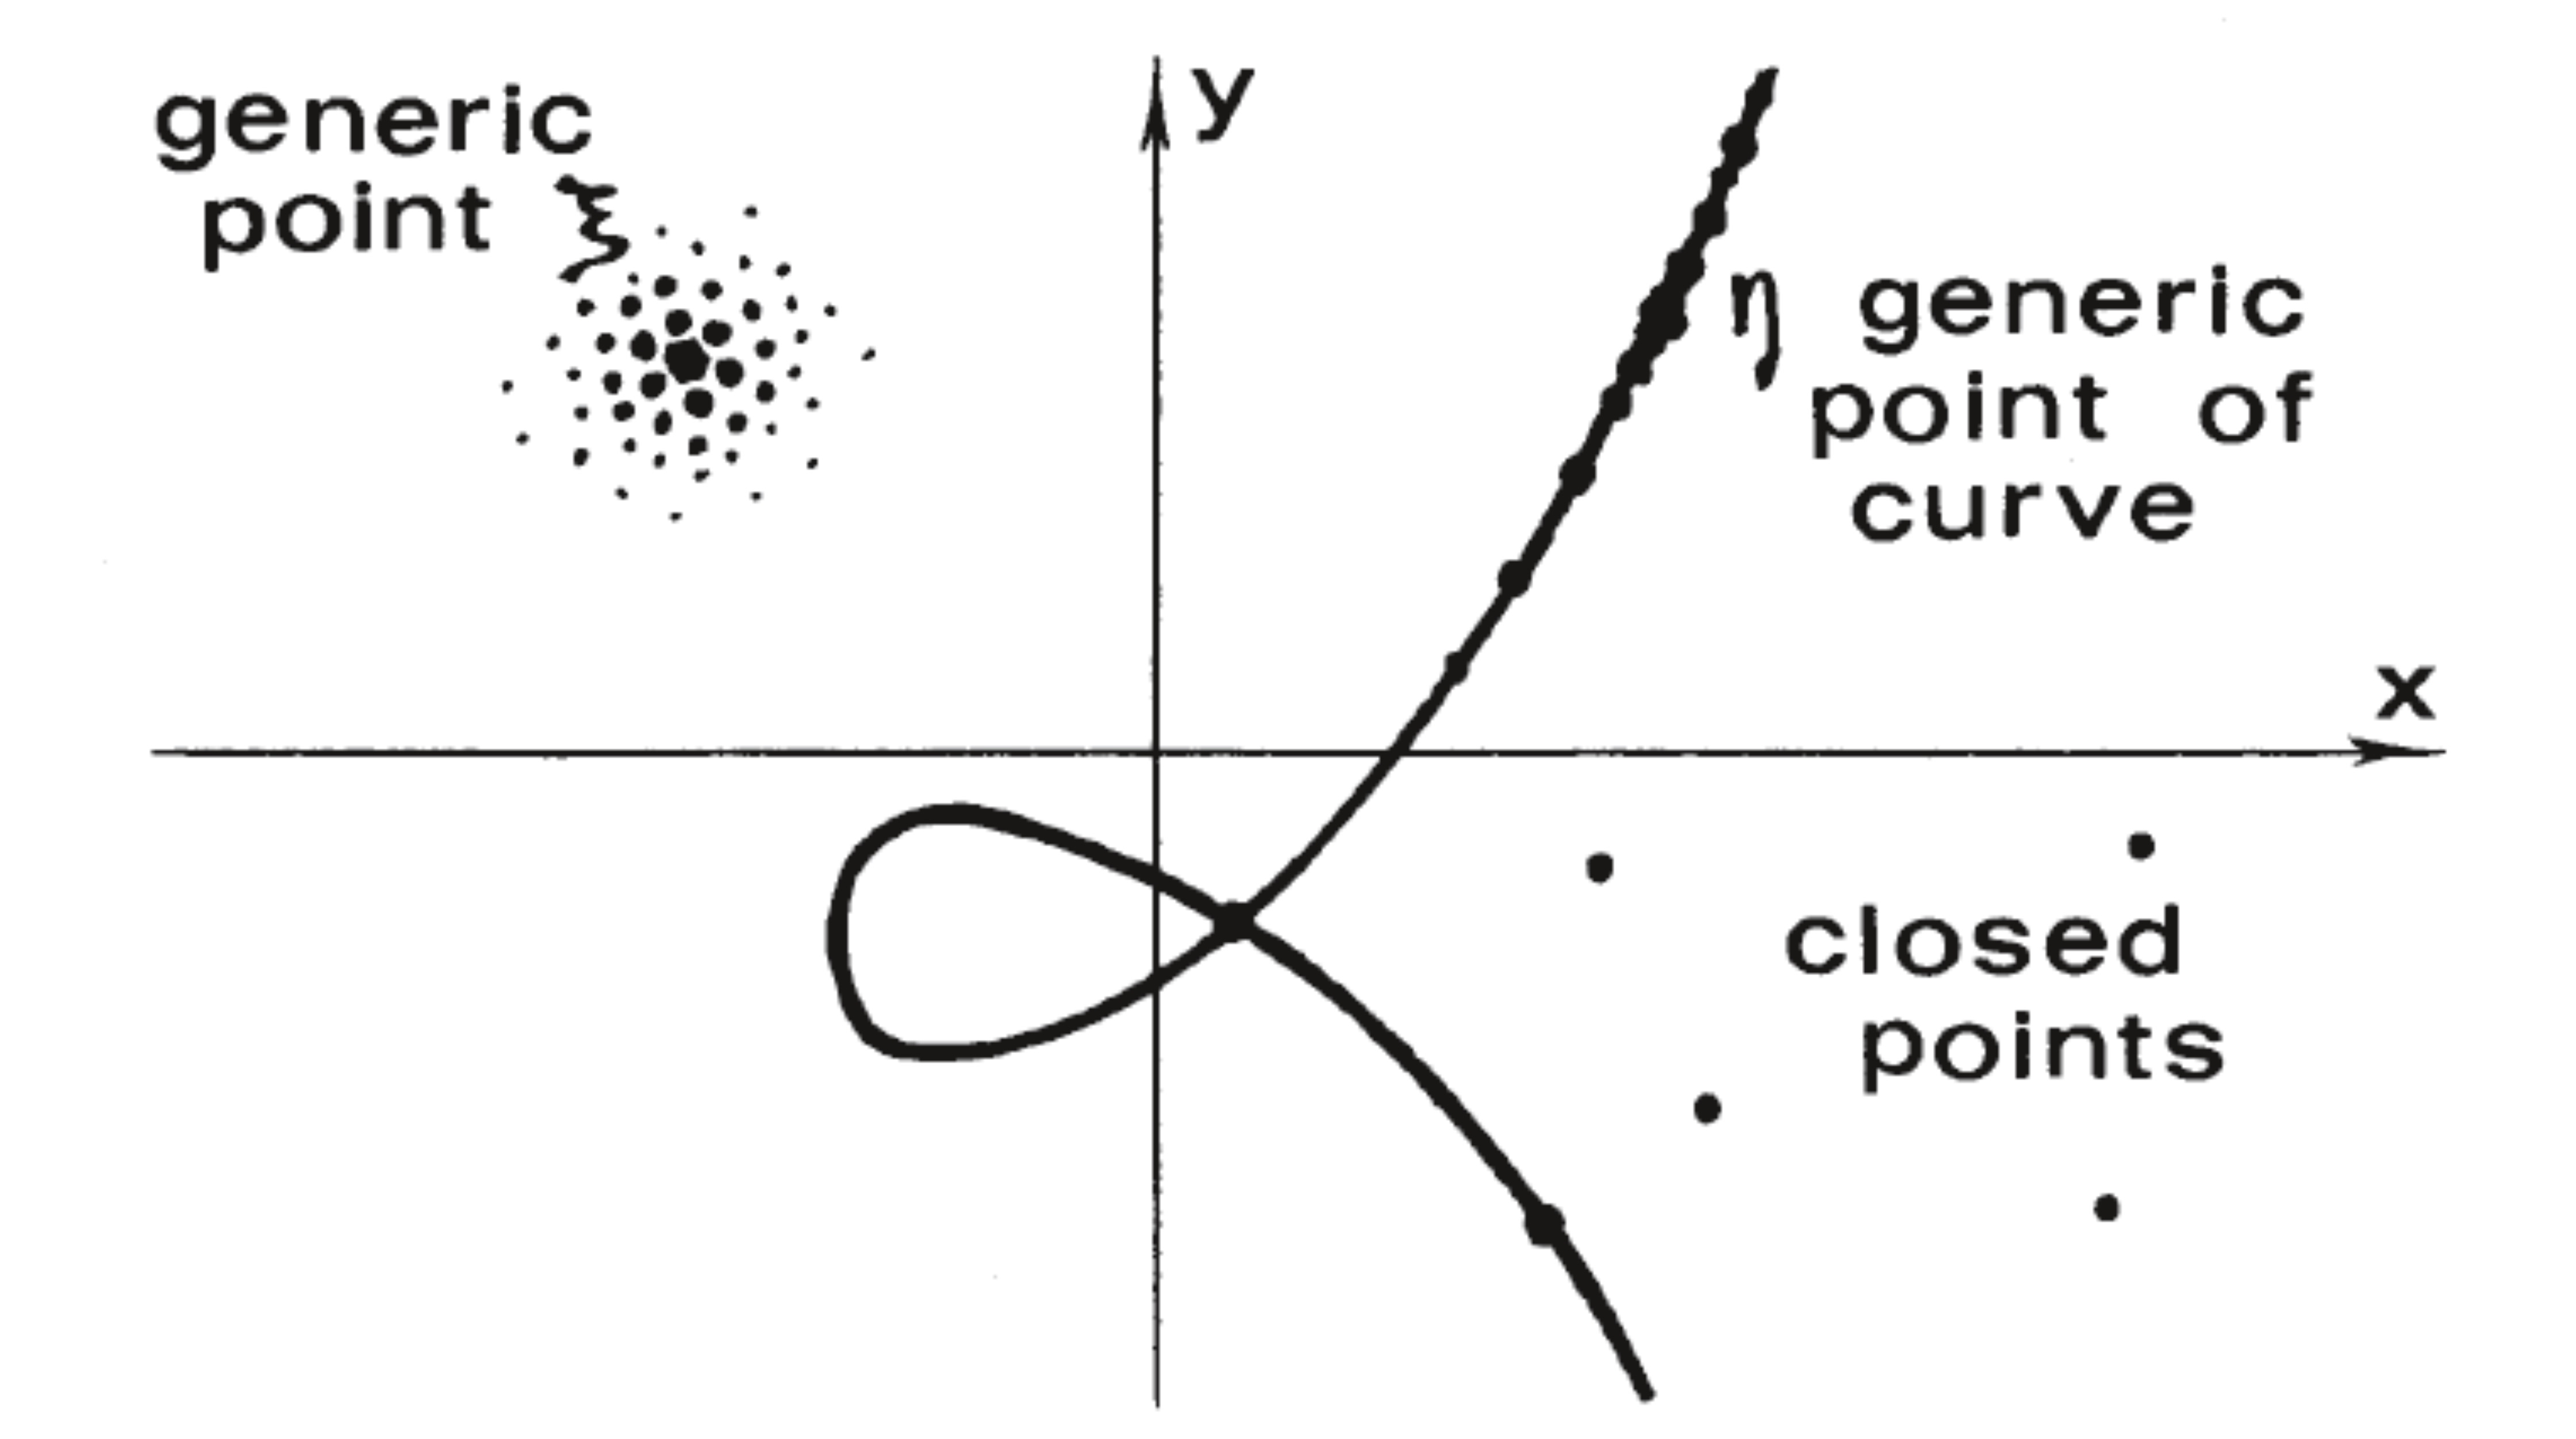
\includegraphics[width=7cm]{Figure6}\\
	Figure 6. $\Spec k[x,y]$
	\end{center}
	
	
	%Example 2.3.5
	\begin{example}
	%
		\tn{$X_1,X_2$가 스킴이며 $U_1\bseq X_1,U_2\bseq X_2$가 열린 부분집합이고
		$\ph:(U_1,\mc O_{X_1}\rest_{U_1})\ra(U_2,\mc O_{X_2}\rest_{U_2})$가 국소환 달린 공간 동형사상이라 하자.
		그 경우 우리는 $X_1$과 $X_2$를 $U_1$과 $U_2$를 따라 동형사상 $\ph$를 통해
		\tb{붙이는(glueing)} 것으로 얻어진 스킴 $X$를 정의할 수 있다.
		$X$의 위상공간은 분리합집합 $X_1\cup X_2$의 동치 관계 $x_1\sim\ph(x_1)\:(x_1\in U_1)$ 하에서의 몫공간이며 몫위상을 가진다.
		그러므로 함수 $i_1:X_1\ra X$와 $i_2:X_2\ra X$가 존재하여 부분집합 $V\bseq X$가 열린집합일 필요충분조건은
		$i_1^{-1}(V)$가 $X_1$에서 열려 있으며 $i_2^{-1}(V)$가 $X_2$에서 열려 있는 것이도록 한다.
		구조층 $\mc O_X$는 다음과 같이 정의된다: 임의의 열린집합 $V\bseq X$에 대하여,}
	%
		$$\mc O_X(V)=\sx{\bk{s_1,s_2}}{s_1\in\mc O_{X_1}(i_1^{-1}(V)),s_2\in\mc O_{X_2}(i_2^{-1}(V)),
		\ph(s_1\rest_{i_1^{-1}(V)\cap U_1})=s_2\rest_{i_2^{-1}(V)\cap U_2}}$$
	%
		\tn{이제 $\mc O_X$가 층이며 $(X,\mc O_X)$가 국소환 달린 공간임은 명확하다.
		이에 더해 $X_1$과 $X_2$가 스킴이므로 $X$의 모든 점이 아핀 근방을 가지며 따라서 $X$는 스킴이다.}
	%
	\end{example}
	
	
	%Example 2.3.6
	\begin{example}
	%
		\tn{붙임의 예로 $k$가 체이며 $X_1=X_2=\mb A_k^1$이며 극대 아이디얼 $(x)$에 대응하는 점 $P$에 대하여
		$U_1=U_2=\mb A_k^1-\{P\}$이고 $\ph:U_1\ra U_2$가 항등함수라 하자.
		$X$가 $X_1$과 $X_2$를 $U_1$과 $U_2$를 따라 $\ph$를 통해 붙여 얻어진 공간이라 하자.
		우리는 `점 $P$가 중복된 아핀 직선'을 얻는다.\\
		이는 아핀 스킴이 아닌 스킴의 예이다(!). 또한 이는 나중에 (4.0.1)에서 보게 될 비분리 스킴의 예이다.}
	%
	\end{example}
	
	다음으로 우리는 등급환들로부터 구축된 사영 대수다양체와 유사한 스킴들의 중요한 족을 정의할 것이다.
	
	$S$가 등급환이라 하자. 등급환에 관한 관습에 대해서는 (I, \S 2)를 참조하라. 아이디얼 $\bigoplus_{d>0}S_d$를 $S_+$로 표기한다.
	
	\ti{집합} $\Proj S$를 $S_+$ 전체를 포함하지는 않는 모든 동급 소 아이디얼 $\mf p$들의 집합으로 정의한다.
	만약 $\mf a$가 $S$의 동급 아이디얼이면 부분집합 $V(\mf a)=\sx{\mf p\in\Proj S}{\mf p\pseq\mf a}$로 정의한다.
	
	
	%Lemma 2.4
	\begin{lemma}
	%
		\tn{\begin{enumerate}[label=(\alph*)]
		\item 만약 $\mf a$와 $\mf b$가 $S$에서의 동급 아이디얼들이면 $V(\mf a\mf b)=V(\mf a)\cup V(\mf b)$이다.
		\item 만약 $\{\mf a_i\}$가 $S$에서의 동급 아이디얼들의 족이면 $V(\sum\mf a_i)=\bigcap V(\mf a_i)$이다.
		\end{enumerate}}
	%
		\tn{\\\pf 동급 아이디얼 $\mf p$가 소 아이디얼일 필요충분조건은 임의의 두 \ti{동급} 원소 $a,b\in S$에 대하여
		$ab\in\mf p$가 $a\in\mf p$ 또는 $b\in\mf p$인 것이라는 사실을 사용하면 증명은 (2.1a,b)의 증명과 같다.}
	%
	\qed
	%
	\end{lemma}
	
	이 보조정리에 의해 우리는 $\Proj S$ 상에 닫힌집합들이 $V(\mf a)$ 형태의 부분집합들이도록 하는 위상을 정의할 수 있다.
	
	다음으로 우리는 $\Proj S$ 상에서의 환의 층 $\mc O$를 정의할 것이다.
	각각의 $\mf p\in\Proj S$에 대하여 $T$가 $\mf p$에 속하지 않는 $S$의 모든 \ti{동급} 원소들로 구성된 곱셈적 계라 하고
	국소화 환 $T^{-1}S$에 속한 등급 0인 원소들로 구성된 환 $S_{(\mf p)}$를 고려하자.
	임의의 열린 부분집합 $U\bseq\Proj S$에 대하여 $\mc O(U)$를
	각각의 $\mf p\in U$에 대하여 $s(\mf p)\in S_{(\mf p)}$이며 국소적으로 $S$의 원소들의 몫인
	(각각의 $\mf p\in U$에 대하여 $U$에서의 $\mf p$의 근방 $V$와 $S$의 동일한 등급의 동급 원소 $a,f$가 존재하여
	모든 $\mf q\in V$에 대하여 $f\notin\mf q$이며 $S_{(\mf q)}$에서 $s(\mf q)=a/f$를 만족시킨다)
	함수 $s:U\ra\coprod S_{(\mf p)}$들의 집합으로 정의한다.
	이제 $\mc O$가 자연스러운 제한함수들을 가지는 환의 준층임은 명확하며 정의의 국소적 본질에 의해 $\mc O$가 층이다.
	
	
	%Definition
	\begin{definition}
	%
		\tn{만약 $S$가 임의의 등급환이면 $(\Proj S,\mc O)$를 위에서 구축된 환의 층을 가지는 위상공간으로 정의한다.}
	%
	\end{definition}
	
	
	%Proposition 2.5
	\begin{proposition}
	%
		\tn{$S$가 등급환이라 하자.
	%
		\begin{enumerate}[label=(\alph*)]
		\item 임의의 $\mf p\in\Proj S$에 대하여 줄기 $\mc O_{\mf p}$는 국소환 $S_{(\mf p)}$와 동형이다.
		\item 임의의 동급원 $f\in S_+$에 대하여 $D_+(f)=\sx{\mf p\in\Proj S}{f\notin\mf p}$라 하자.
		그 경우 $D_+(f)$는 $\Proj S$에서 열려 있다. 이에 더해 이러한 열린집합들은 $\Proj S$를 덮으며
		이러한 각각의 열린집합에 대하여 다음과 같은 국소환 달린 공간 동형사상이 존재한다.
	%
		$$(D_+(f),\mc O\rest_{D_+(f)})\cong\Spec S_{(f)}$$
	%
		여기에서 $S_{(f)}$는 국소화 환 $S_f$에서의 등급 0인 원소들의 부분환이다.
		\item $\Proj S$는 스킴이다.
		\end{enumerate}}
	%
		\tn{\\\pf 먼저 (a)는 $\Proj S$가 국소환 달린 공간임을 말해주며 (b)는 이것이 열린 아핀 스킴들에 의해 덮임을 말해주므로
		(c)는 (a)와 (b)의 결과이다.\\
		(a)의 증명은 위의 (2.2a)의 증명과 거의 동일하며 독자에게 남긴다.\\
		(b)를 증명하기 위해 먼저 $D_+(f)=\Proj S-V((f))$가 열린집합임을 기억해 두라.
		$\Proj S$의 원소들이 $S_+$ 전체를 포함하지는 않는 $S$의 동급 소 아이디얼 $\mf p$들이므로
		동급원 $f\in S_+$에 대한 열린집합 $D_+(f)$들이 $\Proj S$를 덮음이 따라온다. 이제 동급원 $f\in S_+$를 고정하자.
		우리는 $D_+(f)$에서 $\Spec S_{(f)}$로의 국소환 달린 공간 동형사상 $(\ph,\ph^\#)$를 정의할 것이다.
		자연스러운 환 준동형사상 $S\ra S_f$가 존재하며 $S_{(f)}$는 $S_f$의 부분환이다.
		임의의 동차 아이디얼 $\mf a\bseq S$에 대하여 $\ph(\mf a)=(\mf aS_f)\cap S_{(f)}$라 하자.
		특히 만약 $\mf p\in D_+(f)$이면 $\ph(\mf p)\in\Spec S_{(f)}$이며 따라서 이는 집합론적 함수로서 $\ph$를 제공한다.
		국소화의 성질은 $\ph$가 $D_+(f)$에서 $\Spec S_{(f)}$로의 함수로서 전단사임을 보여준다.
		이에 더해 만약 $\mf a$가 $S$의 동급 아이디얼이면 $\mf p\pseq\mf a$일 필요충분조건은 $\ph(\mf p)\pseq\ph(\mf a)$인 것이다.
		따라서 $\ph$는 위상동형사상이다.
		또한 만약 $\mf p\in D_+(f)$이면 국소환 $S_{(\mf p)}$와 $(S_{(f)})_{\ph(\mf p)}$가 자연스럽게 동형임을 기억해 두라.
		이러한 동형사상들과 위상동형사상 $\ph$는 자연스러운 층 사상
		$\ph^\#:\mc O_{\Spec S(f)}\ra\ph_*(\mc O_{\Proj S}\rest_{D^+(f)})$를 유도하며 이것이 동형사상임을 즉시 밝힐 수 있다.
		따라서 $(\ph,\ph^\#)$는 요구된 것과 같이 국소환 달린 공간 동형사상이다.}
	%
	\qed
	%
	\end{proposition}
	
	
	%Example 2.5.1
	\begin{example}
	%
		\tn{만약 $A$가 환이면 $A$ 상에서의 \tb{사영 $n$-공간(projective $n$-space)}을 스킴\\
		$\Pn_A=\Proj A[x_0,\ldots,x_n]$으로 정의한다.
		특히 만약 $A$가 대수적으로 닫힌 체 $k$이면 $\Pn_k$는 스킴이며 그 닫힌점들로 구성된 부분공간은
		사영 $n$-공간이라 불리는 \ti{대수다양체}와 자연스럽게 동형이다 - 아래의 (Ex. 2.14d)를 참조하라.}
	%
	\end{example}
	
	다음으로 우리는 스킴의 개념이 실제로 대수다양체의 개념을 일반화함을 보일 것이다. 대수다양체가 스킴이라는 것은 사실이 아니다.
	우리가 위 예에서 관찰한 것과 같이 $\mb A^1_k$ 또는 $\mb A^2_k$와 같은 스킴의 기반 위상공간은
	대응하는 대수다양체보다 더 많은 점을 가진다.
	그러나 대수다양체의 모든 기약 부분집합에 일반점들을 추가하여 스킴으로 만드는 자연스러운 방법이 존재함을 보일 것이다. (Ex. 2.9)
	
	결과를 진술하기 위해서는 정의가 필요하다.
	
	
	%Definition
	\begin{definition}
	%
		\tn{$S$가 고정된 스킴이라 하자. \tb{$S$ 상에서의 스킴(Scheme over $S$)}은 사상 $X\ra S$를 가지는 스킴 $X$이다.
		만약 $X$와 $Y$가 $S$ 상에서의 스킴이면 $X$에서 $Y$로의 $S$ 상에서의 스킴으로서의 사상은($S$-사상이라고도 불린다)
		$S$로의 주어진 사상과 호환되는 사상 $f:X\ra Y$이다. $S$ 상에서의 스킴들의 범주를 $\Sch S$로 표기한다.
		만약 $A$가 환이면 표기법을 남용하여 $\Spec A$ 상에서의 스킴들의 범주를 $\Sch A$로 표기한다.}
	%
	\end{definition}
	
	
	%Proposition 2.6
	\begin{proposition}
	%
		\tn{$k$가 대수적으로 닫힌 체라 하자. $k$ 상에서의 대수다양체의 범주에서 $k$ 상에서의 스킴의 범주로의
		자연스러운 충실충만한 함자 $t:\mf{Var}(k)\ra\Sch k$가 존재한다.
		임의의 대수다양체 $V$에 대하여 그 위상공간은 $\mrm{sp}(t(V))$의 닫힌점들의 집합과 위상동형이며
		그 정칙 함수층은 $t(V)$의 구조층을 이러한 위상동형사상에 의해 제한하는 것으로 얻어진다.\\\\
	%
		\pf 먼저 $X$가 임의의 위상공간이며 $t(X)$가 $X$의 (공집합이 아닌) 기약 닫힌 부분집합들의 집합이라 하자.
		만약 $Y$가 $X$의 닫힌 부분집합이면 $t(Y)\bseq t(X)$이다.
		이에 더해 $t(Y_1\cup Y_2)=t(Y_1)\cup t(Y_2)$이며 $t(\bigcap Y_i)=\bigcap t(Y_i)$
		그러므로 우리는 $t(Y)$ ($Y$는 $X$의 닫힌 부분집합) 형태의 부분집합들을 닫힌집합으로 취하는 것으로
		$t(X)$ 상에 위상을 정의할 수 있다. 만약 $f:X_1\ra X_2$가 연속 함수이면 우리는 기약 닫힌집합을
		그 상의 폐포로 대응시키는 함수 $t(f):t(X_1)\ra t(X_2)$를 얻는다. 그러므로 $t$는 위상공간의 범주 상에서의 함자이다.
		이에 더해 우리는 연속 함수 $X\ra t(X)$를 $\al(P)=\overline{\{P\}}$로 정의할 수 있다.
		$\al$가 $X$의 열린 부분집합들의 집합과 $t(X)$의 열린 부분집합들의 집합 간의 전단사 함수를 유도함을 기억해 두라.\\
		이제 $k$가 대수적으로 닫힌 체라 하자. $V$가 $k$ 상에서의 대수다양체이며 $\mc O_V$가 그 정칙 함수층이라 하자. (1.0.1)
		우리는 $(t(V),\al_*(\mc O_V)$가 $V$ 상에서의 스킴임을 보일 것이다.
		임의의 대수다양체가 열린 아핀 부분대수다양체들로 덮일 수 있으므로 (I, 4.3)
		$V$가 아핀이면 $(t(V),\al_*(\mc O_V))$가 스킴임을 보이면 충분하다.
		따라서 $V$가 아핀 대수다양체이며 아핀 좌표환 $A$를 가진다 하자. 국소환 달린 공간 사상}
	%
		$$\be:(V,\mc O_V)\ra X=\Spec A$$
	%
		\tn{를 다음과 같이 정의한다: 각각의 점 $P\in V$에 대하여 $\be(P)=\mf m_P$%
		($P$에서 소멸하는 모든 정칙 함수들로 구성된 $A$의 아이디얼)라 하자.
		그 경우 (I, 3.2b)에 의해 $\be$는 $V$에서 $X$의 닫힌점들의 집합으로의 전단사 함수이다.
		이제 임의의 열린집합 $U\bseq X$에 대하여 환 준동형사상 $\mc O_X(U)\ra\be_*(\mc O_V)(U)=\mc O_V(\be^{-1}U)$를 정의할 것이다.
		주어진 단면 $s\in\mc O_X(U)$와 주어진 점 $P\in\be^{-1}(U)$에 대하여
		$s$의 줄기 $\mc O_{X,\be(P)}$(이는 국소환 $A_{\mf m_P}$와 동형이다)에서의 상을 취하고
		몫환 $A_{\mf m_P}/\mf m_P$(이는 $k$와 동형이다)로 보내는 것으로 $S(P)$를 정의한다.
		이것이 정칙 함수임을 간단히 보일 수 있으며 따라서 이러한 함수는 동형사상 $\mc O_X(U)\cong O_V(\be^{-1}U)$를 제공한다.
		마지막으로 $A$의 소 아이디얼들이 $V$의 기약 닫힌 부분집합들과 일대일 대응하므로 ((I.1.4)와 증명을 참조하라)
		이러한 언급들은 $(X,\mc O_X)$가 $(t(V),\al_*\mc O_V)$와 동형임을 보여주며 따라서 후자는 실제로 아핀 스킴이다.\\
		$(t(V),\al_*\mc O_V)$에서 $\Spec k$로의 사상을 제시하기 위해서는 환 준동형사상
		$k\ra\Ga(t(V),\al_*(\mc O_V))=\Ga(V,\mc O_V)$를 제시하면 충분하다.
		우리는 $\lm\in k$를 $V$ 상에서의 상수함수 $\lm$로 대응시킨다. 그러므로 $t(V)$는 $k$ 상에서의 스킴이 된다.
		마지막으로 만약 $V$와 $W$가 대수다양체이면 다음의 자연스러운 함수가 전단사임을 간단히 확인할 수 있다. (Ex. 2.15)}
	%
		$$\Hom_{\mf{Var}(k)}(V,W)\ra\Hom_{\Sch k}(t(V),t(W))$$
	%
		\tn{이는 함자 $t:\mf{Var}(k)\ra\Sch k$가 충실충만함을 보여준다.
		특히 이는 $t(V)$가 $t(W)$와 동형일 필요충분조건이 $V$가 $W$와 동형인 것임을 함의한다.\\
		$\al:V\ra t(V)$가 $V$에서 $t(V)$의 닫힌점들의 (유도 위상을 가지는) 집합으로의 위상동형사상을 유도함은 구축에 의해 명백하다.}
	%
	\qed
	%
	\end{proposition}
	
	\ti{Note.} 나중에 (4.10)에서 함자 $t$의 상이 정확히 무엇인지를 보게 될 것이다.
	
	
	\subsection*{Exercises (연습문제)}
	
	
	\begin{enumerate}[label=\tb{2.\arabic*.},itemindent=0mm,itemsep=2mm]
	\item $A$가 환이고 $X=\Spec A$이며 $f\in A$이고 $D(f)\bseq X$가 $V((f))$의 여집합인 열린집합이라 하자.
	국소환 달린 공간 $(D(f),\mc O_X\rest_{D(f)})$가 $\Spec A_f$와 동형임을 보여라.
	\item $(X,\mc O_X)$가 스킴이며 $U\bseq X$가 임의의 열린 부분집합이라 하자.
	$(U,\mc O_X\rest_U)$가 스킴임을 보여라. 우리는 이를 열린집합 $U$ 상에서의 \tb{유도 스킴 구조(induced scheme structure)}라 부르며
	$(U,\mc O_X\rest_U)$를 $X$의 \tb{열린 부분스킴(open subscheme)}이라 한다.
	\item \tb{축약 스킴.} 스킴 $(X,\mc O_X)$가 \tb{축약(reduced)}이라는 것의 정의는
	모든 열린집합 $U\bseq X$에 대하여 환 $\mc O_X(U)$가 멱영원을 갖지 않는 것이다.
	\begin{enumerate}[label=(\alph*)]
	\item $(X,\mc O_X)$가 축약일 필요충분조건은 모든 $P\in X$에 대하여 국소환 $\mc O_{X,P}$가 멱영원을 갖지 않는 것임을 보여라.
	\item $(X,\mc O_X)$가 스킴이라 하자. $(\mc O_X)_{\mrm{red}}$가 준층 $U\mt\mc O_X(U)_{\mrm{red}}$에 연관된 층이라 하자.
	(여기에서 임의의 환 $A$에 대하여 $A$의 자신의 멱영원들의 아이디얼에 대한 몫을 $A_{\mrm{red}}$로 표기한다.)
	$(X,(\mc O_X)_{\mrm{red}})$가 스킴임을 보여라.
	우리는 이를 $X$에 연관된 \tb{축약 스킴(reduced scheme)}이라 부르며 $X_{\mrm{red}}$로 표기한다.
	기반 위상공간의 상에서 위상동형사상인 스킴 사상 $X_{\mrm{red}}\ra X$가 존재함을 보여라.
	\item $f:X\ra Y$가 스킴 사상이며 $X$가 축약이라 가정하자.
	유일한 사상 $g:X\ra Y_{\mrm{red}}$가 존재하여 $f$가 $g$와 자연스러운 사상 $Y_{\mrm{red}}\ra Y$의 합성이도록 한다.
	\end{enumerate}
	\item $A$가 환이며 $(X,\mc O_X)$가 스킴이라 하자. 사상 $f:X\ra\Spec A$가 주어진 경우
	층 상에서의 연관된 사상 $f^\#:\mc O_{\Spec A}\ra f_*\mc O_X$가 존재한다.
	대역적 단면을 취하면 준동형사상 $A\ra\Ga(X,\mc O_X)$를 얻는다. 그러므로 다음과 같은 자연스러운 함수가 존재한다.
	%
	$$\al:\Hom_{\mf{Sch}}(X,\Spec A)\ra\Hom_{\mf{Ring}}(A,\Ga(X,\mc O_X))$$
	%
	$\al$가 전단사임을 보여라. (cf. (I, 3.5)가 대수다양체에 대한 유사한 진술이다.)
	\item $\Spec\Z$를 기술하고 이것이 스킴의 범주에서의 끝 대상임을 보여라.
	i.e. 각각의 스킴 $X$에서 $\Spec\Z$로의 유일한 사상이 존재한다.
	\item 자명환의 스펙트럼을 기술하고 이것이 스킴의 범주에서의 시작 대상임을 보여라.
	(우리의 관습에 의하면 모든 환 준동형사상은 $1$을 $1$로 대응시켜야 한다.
	자명환에서 $0=1$이므로 우리는 각각의 환 $R$에서 자명환으로의 유일한 준동형사상이 존재함을 알 수 있지만
	$R$에서 $0=1$이 아닌 한 자명환에서 $R$로의 준동형사상은 존재하지 않는다.)
	\item $X$가 스킴이라 하자. 임의의 $x\in X$에 대하여 $\mc O_x$가 $x$에서의 국소환이고 $\mf m_x$가 그 극대 아이디얼이라 하자.
	$x$의 $X$ 상에서의 \tb{잉여류체(residue field)}를 체 $k(x)=\mc O_x/\mf m_x$로 정의한다. 이제 $K$가 임의의 체라 하자.
	$\Spec K$에서 $X$로의 사상을 제시하는 것은 점 $x\in X$와 포함사상 $k(x)\ra K$를 제시하는 것과 동치임을 보여라.
	\item $X$가 스킴이라 하자. 임의의 점 $x\in X$에 대하여 $X$의 $x$에서의 \tb{Zariski 접공간(Zariski tangent space)} $T_x$를
	$k(x)$-벡터 공간 $\mf m_x/\mf m_x^2$의 쌍대로 정의한다.
	이제 $X$가 체 $k$ 상에서의 스킴이며 $k[\ep]/\ep^2$가 $k$ 상에서의 \tb{이원수환(ring of dual numbers)}이라 하자.
	$\Spec k[\ep]/\ep^2$에서 $X$로의 $k$-사상을 제시하는 것이
	\tb{$k$ 상에서 유리(rational over $k$)}(i.e. $k(x)=k$)인 점 $x\in X$와 $T_x$의 원소를 제시하는 것과 동치임을 보여라.
	\item 만약 $X$가 위상공간이며 $Z$가 $X$의 기약 닫힌집합이면 $Z$에 대한 \tb{일반점(generic point)}은
	$Z=\overline{\{\ze\}}$를 만족시키는 점 $\ze$이다.
	만약 $X$가 스킴이면 모든 (공집합이 아닌) 기약 닫힌 부분집합이 유일한 일반점을 가짐을 보여라.
	\item $\Spec\R[x]$를 기술하라. 그 위상공간을 집합 $\R$과 $\C$와 비교하면 어떠한가?
	\item $k=\mb F_p$가 $p$개 원소를 가지는 유한체라 하자. $\Spec k[x]$를 기술하라. 그 점들의 잉여류체가 무엇인가?
	주어진 잉여류체를 가지는 점들은 얼마나 존재하는가?
	\item \tb{붙임 보조정리.} 본문(2.3.5)에서 기술된 붙임 과정을 다음과 같이 일반화하자.
	$\{X_i\}$가 스킴들의 (무한족일 수 있는) 족이라 하자. 각각의 $i\ne j$에 대하여 열린 부분집합 $U_{ij}\bseq X_i$가 주어졌으며
	이것이 유도 스킴 구조(Ex. 2.2)를 가진다 하자.
	또한 각각의 $i\ne j$에 대하여 스킴 동형사상 $\ph_{ij}:U_{ij}\ra U_{ji}$가 주어졌으며
	(1) 각각의 $i,j$에 대하여 $\ph_{ji}=\ph_{ij}^{-1}$이고
	(2) 각각의 $i,j,k$에 대하여 $\ph_{ij}(U_{ij}\cap U_{ik})=U_{ji}\cap U_{jk}$이며
	$U_{ij}\cap U_{ik}$ 상에서 $\ph_{ik}=\ph_{jk}\circ\ph_{ij}$라 하자.
	그 경우 스킴 $X$와 각각의 $i$에 대한 사상 $\psi_i:X_i\ra X$들이 존재하여
	(1) $\psi_i$가 $X_i$에서 $X$의 열린 부분스킴으로의 동형사상이며
	(2) $\psi_i(X_i)$들이 $X$를 덮고
	(3) $\psi_i(U_{ij})=\psi_i(X_i)\cap\psi_j(X_j)$이며
	(4) $U_{ij}$ 상에서 $\psi_i=\psi_j\circ\ph_{ij}$가 성립한다.
	우리는 $X$가 스킴 $X_i$들을 동형사상 $\ph_{ij}$들을 따라 \tb{붙이는(glueing)} 것으로 얻어졌다 한다.
	흥미로운 특수한 경우는 족 $X_i$가 임의로 주어졌으며 $U_{ij}$들과 $\ph_{ij}$들이 모두 공집합과 공함수인 경우이다.
	그 경우 스킴 $X$는 $X_i$들의 \tb{분리합집합(disjoint union)}이라 불리며 $\coprod X_i$로 표기된다.
	\item 위상공간이 \tb{준컴팩트(quasi-compact)}임은 모든 열린 덮개가 유한 부분덮개를 가지는 것이다.
	\begin{enumerate}[label=(\alph*)]
	\item 위상공간이 Noether(I. \S 1)일 필요충분조건은 모든 열린 부분집합이 준컴팩트인 것임을 보여라.
	\item 만약 $X$가 아핀 스킴이면 $\sp(X)$가 준컴팩트이지만 일반적으로 Noether는 아님을 보여라.
	만약 $\sp(X)$가 준컴팩트이면 스킴 $X$가 \tb{준컴팩트(quasi-compact)}라 한다.
	\item 만약 $A$가 Noether 환이면 $\sp(\Spec A)$가 Noether 위상공간임을 보여라.
	\item $A$가 Noether가 아닌 경우에도 $\sp(\Spec A)$가 Noether일 수 있음을 실례를 통해 보여라.
	\end{enumerate}
	\item \begin{enumerate}[label=(\alph*)]
	\item $S$가 등급환이라 하자. $\Proj S=\es$일 필요충분조건은 $S_+$의 모든 원소가 멱영인 것임을 보여라.
	\item $\ph:S\ra T$가 등급환의 (등급을 보존하는) 등급 준동형사상이라 하자.
	$U=\sx{\mf p\in\Proj T}{\mf p\not\pseq\ph(S_+)}$라 하자.
	$U$가 $\Proj T$의 열린 부분집합이며 $\ph$가 자연스러운 사상 $f:U\ra\Proj S$를 결정함을 보여라.
	\item 사상 $f$는 $\ph$가 동형사상이 아닌 경우에도 동형사상일 수 있다.
	예를 들어 $d_0$가 정수이며 $\ph_d:S_d\ra T_d$가 모든 $d\ge d_0$에 대하여 동형사상이라 하자.
	그 경우 $U=\Proj T$이며 사상 $f:\Proj T\ra\Proj S$가 동형사상임을 보여라.
	\item $V$가 동차 좌표환 $S$를 가지는 사영 대수다양체라 하자. (I, \S 2) $t(V)\cong\Proj S$임을 보여라.
	\end{enumerate}
	\item \begin{enumerate}[label=(\alph*)]
	\item $V$가 대수적으로 닫힌 체 $k$ 상에서의 대수다양체라 하자. 점 $P\in t(V)$가 닫힌점일 필요충분조건은 그 잉여류체가 $k$인 것이다.
	\item 만약 $f:X\ra Y$가 $k$ 상에서의 스킴 사상이며 $P\in X$가 잉여류체 $k$를 가지는 점이면 $f(P)\in Y$도 잉여류체 $k$를 가진다.
	\item 이제 만약 $V,W$가 $k$ 상에서의 임의의 두 대수다양체이면 다음의 자연스러운 함수가 전단사임을 보여라.
	%
	$$\Hom_{\mf{Var}}(V,W)\ra\Hom_{\mf{Sch}/k}(t(V),t(W))$$
	%
	(단사성은 간단하다. 어려운 부분은 이것이 전사임을 보이는 것이다.)
	\end{enumerate}
	\item $X$가 스킴이며 $f\in\Ga(X,\mc O_X)$라 하고 $X_f$가 $f$의 $x$에서의 줄기 $f_x$가
	국소환 $\mc O_x$의 극대 아이디얼 $\mf m_x$에 포함되지 않도록 하는 점 $x\in X$들로 구성된 부분집합이라 하자.
	\begin{enumerate}[label=(\alph*)]
	\item 만약 $U=\Spec B$가 $X$의 열린 \ti{아핀} 부분스킴이며 $\bar f\in B=\Ga(U,\mc O_X\rest_U)$가 $f$의 제한이면
	$U\cap X_f=D(\bar f)$임을 보여라. $X_f$가 $X$의 열린 부분집합이라 결론지어라.
	\item $X$가 준컴팩트라 가정하자. $A=\Ga(X,\mc O_X)$이며 $a\in A$가 $X_f$로의 제한이 0인 원소라 하자.
	어떠한 $n>0$이 존재하여 $f^na=0$을 만족시킴을 보여라. [Hint: $X$의 아핀 열린 덮개를 사용하라.]
	\item 이제 $X$가 각각의 교집합 $U_i\cap U_j$가 준컴팩트하도록 하는 아핀 열린집합 $U_i$들로 구성된 유한 덮개를 가진다 하자.
	(이러한 전제조건은 예를 들어 만약 $\sp(X)$가 Noether인 경우에 만족된다.)
	$b\in\Ga(X_f,\mc O_{X_f})$라 하자. 어떠한 $n>0$에 대하여 $f^nb$가 $A$의 원소의 제한임을 보여라.
	\item (c)의 전제조건 하에서 $\Ga(X_f,\mc O_{X_f})\cong A_f$라 결론지어라.
	\end{enumerate}
	\item \tb{아핀성 판정법.}
	\begin{enumerate}[label=(\alph*)]
	\item $f:X\ra Y$가 스킴 사상이며 $Y$가 열린 부분집합 $U_i$들에 의해 덮이고
	각각의 $i$에 대하여 유도된 사상 $f^{-1}(U_i)\ra U_i$가 동형사상이라 하자. 그 경우 $f$는 동형사상이다.
	\item 스킴 $X$가 아핀일 필요충분조건은 원소들의 유한집합 $f_1,\ldots,f_t\in A=\Ga(X,\mc O_X)$가 존재하여
	열린 부분집합 $X_{f_i}$들이 아핀이고 $f_1,\ldots,f_r$이 $A$에서의 단위 아이디얼을 생성하는 것이다.
	[Hint: 위의 (Ex. 2.4)와 (Ex. 2.16d)를 사용하라.]
	\end{enumerate}
	\item 이 연습문제에서 우리는 환 준동형사상과 환의 스펙트럼의 유도된 사상의 몇 가지 성질들을 비교할 것이다.
	\begin{enumerate}[label=(\alph*)]
	\item $A$가 환이고 $X=\Spec A$이며 $f\in A$라 하자. $f$가 멱영일 필요충분조건은 $D(f)$가 공집합인 것임을 보여라.
	\item $\ph:A\ra B$가 환 준동형사상이며 $f:Y=\Spec B\ra X=\Spec A$가 아핀 스킴의 유도된 사상이라 하자.
	$\ph$가 단사일 필요충분조건은 층 사상 $f^\#:\mc O_X\ra f_*\mc O_Y$가 단사인 것임을 보여라.
	이에 더해 이 경우 $f$가 \tb{우세(dominant)}(i.e. $f(Y)$가 $X$에서 조밀)임을 보여라.
	\item 같은 표기 하에서 만약 $\ph$가 전사이면 $f$가 $Y$에서 $X$의 닫힌 부분집합으로의 위상동형사상이며
	$f^\#:\mc O_X\ra f_*\mc O_Y$가 전사임을 보여라.
	\item (c)의 역을 증명하라. 즉 만약 $f:Y\ra X$가 닫힌 부분집합으로의 위상동형사상이며 $f^\#:\mc O_X\ra f_*\mc O_Y$가 전사이면
	$\ph$가 전사이다. [Hint: $X'=\Spec(A/\ker\ph)$를 고려하고 (b)와 (c)를 사용하라.]
	\end{enumerate}
	\item $A$가 환이라 하자. 다음 조건들이 동치임을 보여라:\\[-2mm]
	\begin{enumerate}[label=(\roman*)]
	\item $\Spec A$가 비연결이다.
	\item 0이 아닌 원소 $e_1,e_2\in A$가 존재하여 $e_1e_2=0,e_1^2=e_1,e_2^2=e_2,e_1+e_2=1$을 만족시킨다.
	(이러한 원소들은 \tb{직교 멱등원(orthogonal idempotent)}들이라 불린다.)
	\item $A$가 두 비자명환의 직접곱 $A_1\times A_2$와 동형이다.
	\end{enumerate}
	\end{enumerate}
	
	
	
	%Section 3
	\section{First Properties of Schemes (스킴의 기본 성질)}
	%
	이 절에서 우리는 스킴의 몇 가지 기본 성질을 제시할 것이다. 특히 우리는 열린 및 닫힌 부분스킴 및 곱 스킴을 논의할 것이다.
	연습문제에서 우리는 구축 가능 집합의 개념을 도입할 것이며 사상의 올의 차원을 연구할 것이다.
	
	
	%Definition
	\begin{definition}
	%
		\tn{스킴이 \tb{연결(connected)}이라는 것의 정의는 그 위상공간이 연결인 것이다.
		스킴이 \tb{기약(irreducible)}이라는 것은 그 위상공간이 기약인 것이다.}
	%
	\end{definition}
	
	
	%Definition
	\begin{definition}
	%
		\tn{스킴 $X$가 \tb{축약(reduced)}이라는 것의 정의는 모든 열린집합 $U$에 대하여 환 $\mc O_X(U)$가 멱영원을 갖지 않는 것이다.
		이와 동치로 (Ex. 2.3) $X$가 축약일 필요충분조건은 모든 $P\in X$에 대하여 국소환 $\mc O_P$들이 멱영원을 갖지 않는 것이다.}
	%
	\end{definition}
	
	
	%Definition
	\begin{definition}
	%
		\tn{스킴 $X$가 \tb{정수적(integral)}이라는 것의 정의는 모든 열린집합 $U\bseq X$에 대하여 환 $\mc O_X(U)$가 정역인 것이다.}
	%
	\end{definition}
	
	
	%Example 3.0.1
	\begin{example}
	%
		\tn{\\만약 $X=\Spec A$가 아핀 스킴이면 $X$가 기약일 필요충분조건은 $A$의 영근기 $\nil A$가 소 아이디얼인 것이다;
		$X$가 축약일 필요충분조건은 $\nil A=0$인 것이다; $X$가 정수적일 필요충분조건은 $A$가 정역인 것이다.}
	%
	\end{example}
	
	
	%Proposition 3.1
	\begin{proposition}
	%
		\tn{\\스킴이 정수적일 필요충분조건은 축약이며 기약인 것이다.\\\\
	%
		\pf 명백히 정수적 스킴은 축약이다. 만약 $X$가 기약이 아니면 공집합이 아닌 서로 소 열린집합 $U_1$과 $U_2$를 찾을 수 있다.
		그 경우 $\mc O(U_1\cup U_2)=\mc O(U_1)\times\mc O(U_2)$이며 이는 정역이 아니다.
		따라서 정수적 스킴임은 기약 스킴임을 함의한다.\\
		역으로 $X$가 축약이며 기약이라 가정하자. $U\bseq X$가 열린집합이며 원소 $f,g\in\mc O(U)$가 존재하여 $fg=0$을 만족시킨다 하자.
		$Y=\sx{x\in U}{f_x\in\mf m_x},Z=\sx{x\in U}{g_x\in\mf m_x}$라 하자.
		그 경우 $Y$와 $Z$는 닫힌집합이며 (Ex 2.16a) $Y\cup Z=U$이다.
		그러나 $X$가 기약이므로 $U$가 기약이고 따라서 $Y$ 또는 $Z$가 $U$와 같다. 일반성을 잃지 않고 $Y=U$라 하자.
		그 경우 $f$의 $U$의 임의의 열린 아핀 부분집합으로의 제한이 멱영이며 (Ex. 2.18a) 따라서 0이고 그러므로 $f$가 0이다.
		이는 $X$가 정수적임을 보여준다.}
	%
		\qed
	%
	\end{proposition}
	
	
	%Definition
	\begin{definition}
	%
		\tn{스킴 $X$가 \tb{국소 Noether(locally Noetherian)}라는 것의 정의는
		각각의 $A_i$가 Noether 환이도록 하는 아핀 열린 부분집합 $\Spec A_i$들로 덮일 수 있는 것이다.
		$X$가 \tb{Noether(Noetherian)}라는 것의 정의는 국소 Noether이며 준컴팩트인 것이다.
		이와 동치로 $X$가 Noether임은 각각의 $A_i$가 Noether 환이도록 하는
		유한 개의 아핀 열린 부분집합 $\Spec A_i$들로 덮일 수 있는 것이다.}
	%
	\end{definition}
	
	
	%Caution 3.1.1
	\begin{caution}
	%
		\tn{\\만약 $X$가 Noether 스킴이면 $\sp(X)$가 Noether 위상공간이지만 그 역은 성립하지 않는다. (Ex. 2.13), (Ex. 3.17)}
	%
	\end{caution}
	
	이러한 정의에서 모든 아핀 열린집합이 Noether 환의 스펙트럼이라 요구하지 않음을 기억해 두라.
	그러므로 Noether 환의 스펙트럼이 Noether 스킴임은 정의에 의해 자명하지만 그 역은 자명하지 않다.
	Noether 성질이 `국소적 성질'임을 보이는 것이 문제이다.
	우리는 앞으로 스킴 또는 스킴 사상의 성질을 정의하면서 종종 유사한 상황을 마주칠 것이며
	따라서 우리는 이러한 상황을 보여주기 위해 Noether 성질의 국소적 본질에 대한 진술과 증명을 조심스럽게 제시할 것이다.
	
	
	%Proposition 3.2
	\begin{proposition}
	%
		\tn{\\스킴 $X$가 국소 Noether일 필요충분조건은 모든 아핀 열린집합 $U=\Spec A$에 대하여 $A$가 Noether 환인 것이다.
		특히 아핀 스킴 $X=\Spec A$가 Noether 스킴일 필요충분조건은 환 $A$가 Noether 환인 것이다.\\\\
	%
		\pf 충분조건임은 정의에서 따라온다.
		그러므로 우리는 $X$가 국소 Noether이며 $U=\Spec A$가 아핀 열린집합이면 $A$가 Noether 환임을 증명해야 한다.
		먼저 만약 $B$가 Noether 환이면 그 임의의 국소화 $B_f$도 그러함을 기억해 두라.
		열린집합 $D(f)\cong\Spec B_f$들은 $\Spec B$의 위상기저를 형성한다.
		따라서 국소 Noether 스킴 $X$ 상에서 Noether 환의 스펙트럼들로 구성된 위상기저가 존재한다.
		특히 우리의 열린집합 $U$는 Noether 환의 스펙트럼들로 덮일 수 있다.\\
		그러므로 우리는 다음 진술을 증명하는 것으로 문제를 줄였다:
		$X=\Spec A$가 아핀 스킴이며 Noether 환의 스펙트럼인 열린집합들로 덮일 수 있다면 $A$가 Noether이다.
		$U=\Spec B$가 $X$의 열린 부분집합이며 $B$가 Noether라 하자. 그 경우 어떠한 $f\in A$에 대하여 $D(f)\bseq U$이다.
		$\bar f$가 $f$의 $B$에서의 상이라 하자. 그 경우 $A_f\cong B_{\bar f}$이며 따라서 $A_f$가 Noether이다.
		그러므로 우리는 $X$를 $A_f$가 Noether이도록 하는 열린 부분집합 $D(f)\cong\Spec A_f$들로 덮을 수 있다.
		$X$가 준컴팩트이므로 이들 중 유한 개가 $X$를 덮는다.\\
		그러므로 우리는 순수히 대수학적인 문제로 문제를 줄였다: $A$가 환이고 $f_1,\ldots,f_r$이 $A$의 유한 개 원소이며
		이들이 단위 아이디얼을 생성하고 각각의 국소화 $A_{f_i}$가 Noether인 경우 $A$가 Noether임을 보여야 한다.
		먼저 보조정리를 수립하겠다. $\mf a\bseq A$가 아이디얼이며 $\ph_i:A\ra A_{f_i}\:(i=1,\ldots,r)$가 국소화 함수라 하자.
		그 경우 다음이 성립한다.}
	%
		$$\mf a=\bigcap\ph_i^{-1}(\ph_i(\mf a)\cdot A_{f_i})$$
	%
		\tn{포함 관계 $\bseq$는 자명하다. 역으로 이러한 교집합에 속한 원소 $b\in A$가 주어진 경우
		각각의 $i$에 대하여 $\ph_i(b)=a_i/f_i^{n_i}\:(a_i\in\mf a,n_i>0)$로 표현 가능하다.
		필요하다면 $n_i$를 증가시키는 것으로 우리는 이들을 모두 고정된 $n$과 같도록 만들 수 있다.
		이는 어떠한 $m_i$에 대하여 $A$에서 다음이 성립함을 의미한다.}
	%
		$$f_i^{m_i}(f_i^nb-a_i)=0$$
	%
		\tn{앞에서와 마찬가지로 모든 $m_i=m$으로 만들 수 있다. 그러므로 각각의 $i$에 대하여 $f_i^{m+n}\in\mf a$이다.
		$f_1,\ldots,f_r$이 단위 아이디얼을 생성하므로 임의의 $N$에 대하여 이들의 $N$승들도 단위 아이디얼을 생성한다.
		$N=n+m$이라 하자. 그 경우 적절한 $c_i\in A$에 대하여 $1=\sum c_if_i^N$이다. 따라서 요구한 것과 같이 다음이 성립한다.}
	%
		$$b=\sum c_if_i^Nb\in\mf a$$
	%
		\tn{이제 우리는 $A$가 Noether임을 간단히 보일 수 있다.
		$\mf a_1\bseq\mf a_2\bseq\cdots$가 $A$에서의 아이디얼들의 상승 연쇄라 하자. 그 경우 각각의 $i$에 대하여}
	%
		$$\ph_i(\mf a_1)\cdot A_{f_i}\bseq\ph_i(\mf a_2)\cdot A_{f_i}\bseq\cdots$$
	%
		\tn{는 $A_{f_i}$에서의 아이디얼들의 상승 연쇄이며 $A_{f_i}$가 Noether이므로 이는 반드시 안정화되어야 한다.
		$A_{f_i}$들이 유한 개이므로 보조정리에 의해 원래 연쇄가 궁극적으로 안정화된다 결론지을 수 있으며 따라서 $A$가 Noether이다.}
	%
		\qed
	%
	\end{proposition}
	
	
	%Definition
	\begin{definition}
	%
		\tn{스킴 사상 $f:X\ra Y$가 \tb{국소유한형(locally of finite type)}이라는 것의 정의는
		아핀 열린집합 $V_i=\Spec B_i$들에 의한 $Y$의 덮개가 존재하여 각각의 $i$에 대하여 $f^{-1}(V_i)$가
		유한생성 $B_i$-대수 $A_{ij}$들에 대한 아핀 열린집합 $U_{ij}=\Spec A_{ij}$들에 의해 덮일 수 있도록 하는 것이다.
		사상 $f$가 \tb{유한형(finite type)}이라는 것의 정의는 추가적으로
		각각의 $f^{-1}(V_i)$가 유한 개의 $U_{ij}$들에 의해 덮일 수 있는 것이다.}
	%
	\end{definition}
	
	
	%Definition
	\begin{definition}
	%
		\tn{사상 $f:X\ra Y$가 \tb{유한(finite)} 사상이라는 것의 정의는 아핀 열린집합 $V_i=\Spec B_i$들에 의한 $Y$의 덮개가 존재하여
		각각의 $i$에 대하여 $f^{-1}(V_i)$가 아핀이며 유한생성 $B_i$-모듈인 $B_i$-대수 $A_i$에 대한 $\Spec A_i$와 일치하는 것이다.}
	%
	\end{definition}
	
	사상 $f:X\ra Y$에 대한 이러한 성질들은 특정한 성질을 가지는 $Y$의 아핀 열린 덮개의 존재성에 의해 정의되었다.
	사실 각각의 경우 이는 $Y$의 모든 아핀 열린집합에 대하여 해당 성질을 요구하는 것과 동치이다. (Ex. 3.1-3.4)
	
	
	%Example 3.2.1
	\begin{example}
	%
		\tn{\\만약 $V$가 대수적으로 닫힌 체 $k$ 상에서의 대수다양체이면 연관된 스킴 $t(V)$((2.6)을 참조하라)는
		$k$ 상에서 유한형인 정수적 Noether 스킴이다: $V$는 유한 개 아핀 열린 부분대수다양체들로 덮일 수 있다. (I, 4.3)
		따라서 $t(V)$는 $\Spec A_i$ 형태의 유한 개 아핀 열린집합들에 의해 덮일 수 있으며
		여기에서 $A_i$는  정역인 유한생성 $k$-대수이므로 Noether이다.}
	%
	\end{example}
	
	
	%Example 3.2.2
	\begin{example}
	%
		\tn{\\만약 $P$가 대수다양체 $V$ 상에서의 점이며 국소환 $\mc O_P$를 가진다 하면
		$\Spec\mc O_P$는 정수적 Noether 스킴이지만 일반적으로 $k$ 상에서 유한형이 아니다.}
	%
	\end{example}
	
	다음으로 우리는 열린 및 닫힌 부분스킴을 다룰 것이다.
	
	
	%Definition
	\begin{definition}
	%
		\tn{스킴 $X$의 \tb{열린 부분스킴(open subscheme)}은 위상공간이 $X$의 열린 부분집합 $U$이며
		구조층 $\mc O_U$가 제한 $\mc O_X\rest_U$와 동형인 스킴 $U$이다.
		\tb{열린 몰입(open immersion)}은 $X$와 $Y$의 열린 부분스킴 간의 동형사상을 유도하는 사상 $f:X\ra Y$이다.}
	%
	\end{definition}
	
	스킴의 모든 열린 부분집합이 유일한 열린 부분스킴 구조를 가짐을 기억해 두라. (Ex. 2.2)
	
	
	%Definition
	\begin{definition}
	%
		\tn{\tb{닫힌 몰입(closed immersion)}은 $\sp(Y)$에서 $\sp(X)$의 닫힌 부분집합으로의 위상동형사상을 유도하며
		$X$ 상에서의 층의 유도된 함수 $f^\#:\mc O_X\ra f_*\mc O_Y$가 전사이도록 하는 스킴 사상 $f:Y\ra X$이다.
		스킴 $X$의 \tb{닫힌 부분스킴(closed subscheme)}은 닫힌 몰입들의 다음 동치 관계 하에서의 동치류이다:
		$f:Y\ra X$와 $f':Y'\ra X$가 동치임은 동형사상 $i:Y'\ra Y$가 존재하여 $f'=f\circ i$를 만족시키는 것이다.}
	%
	\end{definition}
	
	
	%Example 3.2.3
	\begin{example}
	%
		\tn{\\$A$가 환이며 $\mf a$가 $A$의 아이디얼이라 하자. $X=\Spec A$이며 $Y=\Spec A/\mf a$라 하자.
		그 경우 환 준동형사상 $A\ra A/\mf a$는 닫힌 몰입인 스킴 사상 $f:Y\ra X$를 유도한다.
		함수 $f$는 $Y$에서 $X$의 닫힌 부분집합 $V(\mf a)$로의 위상동형사상이며
		구조층의 함수 $\mc O_X\ra f_*\mc O_Y$는 줄기(각각 $A$와 $A/\mf a$의 국소화) 상에서 전사이므로 전사이다.\\
		그러므로 임의의 아이디얼 $\mf a\bseq A$에 대하여 우리는 닫힌집합 $V(\mf a)\bseq X$ 상에서의 닫힌 부분스킴 구조를 얻는다.
		특히 $X$의 모든 닫힌 부분집합 $Y$는 $V(\mf a)=Y$를 만족시키는 모든 아이디얼 $\mf a$들에 대응하는 다수의 부분스킴 구조를 가진다.
		사실 아핀 스킴 $X$의 닫힌 부분집합 $Y$ 상에서의 모든 닫힌 부분스킴 구조는 항상 아이디얼에 의해 이러한 방식으로 등장한다.
		(Ex. 3.11b) 또는 (5.10).}
	%
	\end{example}
	
	
	%Example 3.2.4
	\begin{example}
	%
		\tn{\\더 구체적인 예시를 위해 $k$가 체이며 $A=k[x,y]$라 하자. 그 경우 $\Spec A=\mb A_k^2$는 $k$ 상에서의 아핀 평면이다.
		아이디얼 $\mf a=(xy)$는 $x$축과 $y$축의 합집합으로 구성된 비기약 부분스킴을 준다.
		아이디얼 $\mf a=(x^2)$는 $y$축 상에서 멱영원들을 가지는 부분스킴 구조를 준다.
		아이디얼 $\mf a=(x^2,xy)$는 $y$축 상에 다른 부분스킴 구조를 준다.
		이는 원점에서의 국소환에서만 멱영원을 가진다. 우리는 원점이 이러한 부분스킴에 대한 \tb{매장된 점(embedded point)}이라 한다.}
	%
	\end{example}
	
	
	%Example 3.2.5
	\begin{example}
	%
		\tn{\\$V$가 체 $k$ 상에서의 아핀 대수다양체이며 $W$가 닫힌 부분대수다양체라 하자.
		그 경우 $W$는 $V$의 아핀 좌표환에서의 소 아이디얼 $\mf p$에 대응한다. (I, \S 1) $X=t(V)$와 $Y=t(W)$가 연관된 스킴이라 하자.
		그 경우 $X=\Spec A$이며 $Y$는 $\mf p$에 의해 정의된 닫힌 부분스킴이다.
		각각의 $n\ge 1$에 대하여 $Y_n$이 아이디얼 $\mf p^n$에 대응하는 $X$의 닫힌 부분스킴이라 하자.
		그 경우 $Y_1=Y$이지만 각각의 $n>1$에 대하여 $Y_n$은 닫힌집합 $Y$ 상의 비축약 스킴 구조이다.
		이는 $V$의 어떠한 부분대수다양체에도 대응하지 않는다.
		우리는 $Y_n$을 $Y$의 $X$에서 $n$번째 \tb{무한소 근방(infinitesimal neighborhood)}이라 한다.
		스킴 $Y_n$들은 $Y$의 $X$로의 매장의 성질을 반영한다.
		나중에 (\S9) 우리는 $Y$의 $X$에서의 `형식적 완비화'를 연구할 것이며 이는 대략 $n\ra\infty$에서 스킴 $Y_n$들의 극한이다.}
	%
	\end{example}
	
	
	%Example 3.2.6
	\begin{example}
	%
		\tn{\\$X$가 스킴이며 $Y$가 닫힌 부분집합이라 하자. 일반적으로 $Y$는 가능한 여러 닫힌 부분스킴 구조를 가진다.
		그러나 \tb{축약 유도 닫힌 부분스킴 구조(reduced induced closed subscheme strurcure)}라 불리는
		다른 모든 것보다 `작은' 구조가 존재한다. 이를 기술하겠다.\\
		먼저 $X=\Spec A$가 아핀 스킴이며 $Y$가 닫힌 부분집합이라 하자.
		$\mf a\bseq A$가 $Y$에 속한 모든 소 아이디얼들의 교집합으로 얻어진 아이디얼이라 하자.
		이는 $V(\mf a)=Y$를 만족시키는 최대 아이디얼이다.
		그 경우 우리는 $Y$ 상에서의 축약 유도 구조를 $\mf a$에 의해 정의된 것으로 취한다.\\
		이제 $X$가 임의의 스킴이며 $Y$가 닫힌 부분집합이라 하자. 아핀 열린 부분집합 $U_i\bseq X$들에 대하여
		$U_i$의 닫힌 부분집합 $Y_i=Y\cap U_i$들을 고려하고
		여기에 위 문단에서 아핀 스킴에 대하여 정의된 축약 유도 구조를 부여하자. (이는 $U_i$에 의존할 수 있다.)
		임의의 $i,j$에 대하여 방금 정의한 $Y_i$와 $Y_j$ 상에서의 구조층의 $Y_i\cap Y_j$로의 제한이 동형이며
		이에 더해 모든 $i,j,k$에 대하여 이러한 세 동형사상이 $Y_i\cap Y_j\cap Y_k$ 상에서 호환됨을 주장하겠다.
		이는 $U=\Spec A$가 아핀 열린집합이며 $f\in A$이고 $V=D(f)=\Spec A_f$이면 $A$로부터 얻어진 $Y\cap U$ 상에서의 축약 유도 구조를
		$Y\cap V$로 제한한 것이 $A_f$로부터 얻어진 축약 유도 구조와 일치함을 보이는 것으로 줄어든다.
		이는 만약 $\mf a$가 $Y$에 속한 $A$의 소 아이디얼들의 교집합이면
		$\mf aA_f$가 $Y\cap D(f)$에 속한 $A_f$의 소 아이디얼들의 교집합이라는 대수적 사실에 대응한다.\\
		그러므로 우리는 $Y_i$ 상에서 정의된 층들을 이어붙여 $Y$ 상에서의 층을 얻을 수 있다. (Ex. 1.22)
		이는 $Y$ 상에서의 요구된 축약 유도 부분스킴 구조를 제공한다.
		축약 유도 부분스킴 구조의 보편 성질에 대해서는 아래의 (Ex. 3.11)을 참조하라.}
	%
	\end{example}
	
	
	%Definition
	\begin{definition}
	%
		\tn{스킴 $X$의 \tb{차원(dimension)}은 $\dim X$로 표기되며 위상공간으로서의 차원이다. (I, \S 1)
		만약 $Z$가 $X$의 기약 닫힌 부분집합이면 $Z$의 $X$에서의 \tb{여차원(codimension)}은
		다음과 같은 $Z$에서 시작하는 $X$의 서로 다른 닫힌 기약 부분집합들의 연쇄가 존재하도록 하는 정수 $n$의 상한이다.}
	%
		$$Z=Z_0<Z_1<\cdots<Z_n$$
	%
		\tn{만약 $Y$가 $X$의 임의의 닫힌 부분집합이면 다음과 같이 정의한다.}
	%
		$$\codim(Y,X)=\inf_{Z\bseq Y}\codim(Z,X)$$
	%
		\tn{여기에서 하한은 $Y$의 모든 닫힌 기약 부분집합들에 대하여 취한다.}
	%
	\end{definition}
	
	
	%Example 3.2.7
	\begin{example}
	%
		\tn{\\만약 $X=\Spec A$가 아핀 스킴이면 $X$의 차원은 $A$의 Krull 차원과 같다. (I, \S 1)}
	%
	\end{example}
	
	
	%Caution 3.2.8
	\begin{caution}
	%
		\tn{\\차원과 여차원의 개념을 임의의 스킴에 적용하는 것에는 주의를 기울여야 한다.
		우리의 직관은 체 상에서 유한형인 스킴들을 다루는 것에서 유래하였으며 이 경우 이러한 개념들이 잘 거동한다.
		예를 들어 만약 $X$가 체 $k$ 상에서 유한형인 아핀 정수적 스킴이며 $Y\bseq X$가 임의의 기약 닫힌 부분집합이면
		(I, 1.8A)는 $\dim Y+\codim(Y,X)=\dim X$임을 함의한다.
		그러나 임의의 (심지어 Noether) 스킴 상에서는 웃긴 일이 발생할 수 있다.
	 	(Ex. 3.20-3.22)와 Nagata [7], Grothendieck [EGA IV, \S 5]를 참조하라.}
	%
	\end{caution}
	
	
	%Definition
	\begin{definition}
	%
		\tn{$S$가 스킴이며 $X,Y$가 $S$ 상에서의 스킴(i.e. $S$로의 사상을 가지는 스킴)이라 하자.
		우리는 $X$와 $Y$의 $S$ 상에서의 \tb{올곱(fibred product)}을 $X\times_SY$로 표기하며
		주어진 사상 $X\ra S$ 및 $Y\ra S$와 가환 도표를 형성하며
		다음 성질을 가지는 사상 $p_1:X\times_SY\ra X$와 $p_2:X\times_SY\ra Y$를 가지는 스킴으로 정의한다:
		주어진 $S$ 상에서의 임의의 스킴 $Z$와 위에서 주어진 사상 $X\ra S$ 및 $Y\ra S$와
		가환 도표를 형성하도록 주어진 사상 $f:Z\ra X$ 및 $g:Z\ra Y$에 대하여
		유일한 사상 $\ta:Z\ra X\times_SY$가 존재하여 $f=p_1\circ\ta$이며 $p_2\circ\ta$이다.
		사상 $p_1$과 $p_2$는 올곱에서 그 곱인자로의 \tb{사영사상(projection morphism)}들이라 불린다.}
	%
		$$\begin{tikzcd}[column sep=small]Z\arrow[rrr]\arrow[drr]\arrow[drrrr]&&&X\times_SY\arrow[dl]\arrow[dr]\\
		&&X\arrow[dr]&&Y\arrow[dl]\\
		&&&S\end{tikzcd}$$
	%
		\tn{만약 $X$와 $Y$가 어떠한 기반 스킴 $S$에 대한 언급 없이 주어졌다면 우리는 $S=\Spec\Z$로 취하고 (Ex. 2.5)
		$X$와 $Y$의 \tb{곱(product)}을 $X\times_{\Spec\Z}Y$로 정의한다.}
	%
	\end{definition}
	
	
	%Theorem 3.3
	\begin{theorem}
	%
		\tn{\\스킴 $S$ 상에서의 임의의 두 스킴 $X$와 $Y$에 대하여 올곱 $X\times_SY$가 존재하며 동형 하에서 유일하다.\\\\
	%
		\pf 발상은 먼저 아핀 스킴의 곱을 구축하고 그 후 이어붙이는 것이다. 7개 단계로 진행하겠다.\\
	%
		\tb{Step 1.} $X=\Spec A,Y=\Spec B,S=\Spec R$이 모두 아핀이라 하자. 그 경우 $A$와 $B$는 $R$-대수이다.
		$\Spec(A\otimes_RB)$가 $X$와 $Y$의 $S$ 상에서의 곱임을 주장하겠다.
		임의의 스킴 $Z$에 대하여 (Ex. 2.4)에 의해 $Z$에서 $\Spec(A\otimes_RB)$로의 사상을 제시하는 것은
		$A\otimes_RB$에서 환 $\Ga(Z,\mc O_Z)$로의 준동형사상을 제시하는 것과 같다.
		그러나 $A\otimes_RB$에서 임의의 환으로의 사상을 제시하는 것은 $R$ 상에서 동일한 사상을 유도하는
		$A$와 $B$에서 해당 환으로의 준동형사상들을 제시하는 것과 같다.
		(Ex. 2.4)를 다시 적용하면 $Z$에서 $\Spec(A\otimes_RB)$로의 사상을 제시하는 것은
		$Z$에서 $S$로의 동일한 사상을 유도하는 $Z$에서 $X$ 및 $Z$에서 $Y$로의 사상을 제시하는 것과 같다.
		그러므로 $\Spec(A\otimes_RB)$가 요구된 곱이다.\\
	%
		\tb{Step 2.} 곱의 보편 성질로부터 이것이 (존재하면) 동형 하에서 유일함이 즉시 따라온다.
		앞으로 진행하면서 이미 구축된 곱의 유일성이 필요할 것이다.\\
	%
		\tb{Step 3. 사상 이어붙이기.} 우리는 이미 층(Ex. 1.22)과 스킴(Ex. 2.12)을 어떻게 이어붙이는지를 봤다.
		이제 우리는 사상을 이어붙일 것이다. 만약 $X$와 $Y$가 스킴이면 $X$에서 $Y$로의 사상 $f$를 제시하는 것은
		$X$ 상에서의 열린 덮개 $\{U_i\}$와 각각의 $i,j$에 대하여 $U_i\cap U_j$ 상에서 $f_i$와 $f_j$의 제한이 일치하도록 하는
		사상 $f_i:U_i\ra Y$(여기에서 $U_i$는 유도된 열린 부분스킴 구조를 가진다)들을 제시하는 것과 같다. 증명은 간단하다.\\
	%
		\tb{Step 4.} 만약 $X,Y$가 스킴 $S$ 상에서의 스킴이며 $U\bseq X$가 열린 부분집합이고 곱 $X\times_SY$가 존재한다면
		$p_1^{-1}(U)\bseq X\times_SY$는 $U$와 $Y$의 $S$ 상에서의 곱이다:
		주어진 스킴 $Z$와 사상 $f:Z\ra U$ 및 $g:Z\ra Y$에 대하여 $f$는 포함사상 $U\bseq X$와 합성하면 $Z$에서 $X$로의 사상을 결정한다.
		따라서 사상 $\ta:Z\ra X\times_SY$는 $f,g$ 및 사영들과 호환된다.
		그러나 $f(Z)\bseq U$이므로 $\ta(Z)\bseq p_1^{-1}(U)$이다. 그러므로 $\ta$는 사상 $Z\ra p_1^{-1}(U)$로 간주될 수 있다.
		이는 명백히 유일하며 따라서 $p_1^{-1}(U)$는 곱 $U\times_SY$이다.\\
	%
		\tb{Step 5.} $X,Y$가 $S$ 상에서의 스킴이며 $\{X_i\}$가 $X$의 열린 덮개이고
		각각의 $i$에 대하여 $X_i\times_SY$가 존재한다 하자. 그 경우 $X\times_SY$가 존재한다:
		각각의 $i,j$에 대하여 $X_{ij}=X_i\cap X_j$이며 $U_{ij}\bseq X_i\times_SY$가 $p_1^{-1}(X_{ij})$라 하자.
		Step 4에 의해 $U_{ij}$는 $X_{ij}$와 $Y$의 $S$ 상에서의 곱이다.
		따라서 곱의 유일성에 의해 각각의 $i,j$에 대하여 (유일한) 동형사상 $\ph_{ij}:U_{ij}\ra U_{ji}$가 존재하여 모든 사영과 호환된다.
		이에 더해 이러한 동형사상들은 각각의 $i,j,k$에 대하여 (Ex. 2.12)에서의 의미로 호환된다.
		그러므로 스킴 $X_i\times_SY$들을 동형사상 $\ph_{ij}$들을 통해 붙이면 (Ex. 2.12)에 의해 스킴 $X\times_SY$를 얻는다.
		이것이 실제로 $X$와 $Y$의 $S$ 상에서의 곱임을 주장하겠다.
		사영사상 $p_1$과 $p_2$는 조각 $X_i\times_SY$에서의 사영들을 이어붙이는 것으로 정의된다. (Step 3)
		스킴 $Z$와 사상 $f:Z\ra X,g:Z\ra Y$가 주어졌다 하고 $Z_i=f^{-1}(X_i)$라 하자.
		그 경우 우리는 사상 $\ta_i:Z_i\ra X_i\times_SY$들을 얻으며 따라서 포함사상 $X_i\times_SY\bseq X\times_SY$와 합성하면
		사상 $\ta_i:Z_i\ra X\times_SY$를 얻는다. 이러한 사상들이 $Z_i\cap Z_j$ 상에서 일치함을 검증할 수 있으며
		따라서 이러한 사상들을 이어붙여 (Step 3) 사영들 및 $f$ 및 $g$와 호환되는 사상 $\ta:Z\ra X\times_SY$를 얻는다.
		$\ta$의 유일성은 국소적으로 검증될 수 있다.\\
	%
		\tb{Step 6.} 우리는 Step 1에 의해 만약 $X,Y,S$가 모두 아핀이면 $X\times_SY$가 존재함을 알고 있다.
		그러므로 Step 5를 이용하면 우리는 임의의 $X$와 아핀인 $Y,S$에 대하여 곱이 존재한다 결론지을 수 있다.
		$X$와 $Y$의 역할을 교환하고 Step 5를 다시 적용하면 아핀 $S$ 상에서 임의의 $X$와 $Y$의 곱이 존재함을 알 수 있다.\\
	%
		\tb{Step 7.} 임의의 $X,Y,S$가 주어졌으며 $q:X\ra S,r:Y\ra S$가 주어진 사상이라 하자.
		$S_i$가 $S$의 아핀 열린 덮개라 하자. $X_i=q^{-1}(S_i),Y_i=r^{-1}(S_i)$라 하자.
		그 경우 Step 6에 의해 $X_i\times_{S_i}Y_i$가 존재한다. 이러한 동일한 스킴이 $S$ 상에서 $X_i$와 $Y$의 곱이다:
		$S$ 상에서의 사상 $f:Z\ra X_i$와 $g:Z\ra Y$이 주어진 경우 $g$의 상은 $Y_i$ 내에 포함되어야 한다.
		그러므로 각각의 $i$에 대하여 $X_i\times_SY$가 존재하며 Step 5를 한 번 더 적용하면 $X\times_SY$를 얻는다.
		이는 증명을 완료한다.}
	%
		\qed
	%
	\end{theorem}
	
	아마도 이곳이 올곱의 중요성과 적용에 대한 일반적인 언급을 하기에 좋은 장소인 듯하다.
	먼저 우리는 사상의 올을 정의할 수 있다.
	
	
	%Definition
	\begin{definition}
	%
		\tn{$f:X\ra Y$가 스킴 사상이며 $y\in Y$가 점이라 하자.
		$k(y)$가 $y$의 잉여류체이며 $\Spec k(y)\ra Y$가 자연스러운 사상이라 하자. (Ex. 2.7)
		그 경우 사상 $f$의 점 $y$ 상에서의 \tb{올(fibre)}을 다음의 스킴으로 정의한다.}
	%
		$$X_y=X\times_Y\Spec k(y)$$
	%
	\end{definition}
	
	올 $X_y$는 $k(y)$ 상에서의 스킴이며 우리는 그 기반 위상공간이 $X$의 부분집합 $f^{-1}(y)$와 위상동형임을 보일 수 있다. (Ex. 3.10)
	
	사상의 올의 개념은 사상을 상 스킴의 점들에 의해 매개화된 스킴(올)들의 족으로 간주할 수 있게 해 준다.
	역으로 이러한 족의 개념은 대수적으로 변화하는 스킴의 족의 개념을 유효하게 만드는 좋은 방식이다.
	예를 들어 체 $k$ 상에서의 스킴 $X_0$가 주어진 경우 $X_0$의 \tb{변형들의 족(family of deformations)}을
	$Y$가 연결이며 $k(y_0)=k,X_{y_0}\cong X_0$을 만족시키는 점 $y_0\in Y$가 존재하도록 하는 사상 $f:X\ra Y$로 정의한다.
	$f$의 다른 올 $X_y$들은 $X_0$의 \tb{변형(deformation)}들이라 불린다.
	
	$\Spec\Z$ 상에서의 스킴 $X$에 대한 경우 흥미로운 형태의 족이 등장한다.
	이 경우 일반점 상에서의 올을 취하면 $\Q$ 상에서의 스킴 $X_\Q$를 얻으며
	소수 $p$에 대응하는 닫힌점 상에서의 올을 취하면 유한체 $\mb F_p$ 상에서의 스킴 $X_p$를 얻는다.
	우리는 $X_p$가 스킴 $X$의 법 $p$ \tb{축약(reduction)}에 의해 등장한다고 말한다.\\
	
	올곱의 다른 중요한 응용은 기반 확대의 개념이다. $S$가 (우리가 $S$ 상에서의 스킴들의 범주를 다룬다는 의미로)
	\tb{기반 스킴(base scheme)}으로 간주되는 고정된 스킴이라 하자. 예를 들어 $k$가 체인 경우 $S=\Spec k$에 대해 생각해 보자.
	만약 $S'$이 다른 기반 스킴이며 $S'\ra S$가 사상이면
	$S$ 상에서의 임의의 스킴 $X$에 대하여 $X'=X\times_SS'$은 $S'$ 상에서의 스킴이 될 것이다.
	우리는 $X'$이 $X$로부터 \tb{기반 확대(base extension)} $S'\ra S$에 의해 얻어졌다고 한다.
	예를 들어 $k'$이 $k$의 확대체이며 $S'=\Spec k'$인 경우를 생각해 보자.
	기반 확대가 추이적 연산임을 기억해 두라:
	만약 $S''\ra S'\ra S$가 두 사상이면 $(X\times_SS')\times_{S'}S''\cong X\times_SS''$이다.
	
	이는 대수기하학의 모든 개념을 상대적인 맥락에서 개발하려고 시도해야 한다는
	Grothendieck에 의해 그의 저서 ``El\'ements de G\'eom\'etrie Alg\'ebrique''([EGA])에서 강조된 일반적인 철학과 관련이 있다.
	항상 고정된 기반체 상에서 작업하며 한 번에 하나의 대수다양체의 성질을 고려하는 대신
	우리는 스킴 사상 $f:X\ra S$를 고려하고 사상의 성질을 연구해야 한다.
	그 경우 $f$의 성질들의 기반 확대 하에서의 거동을 연구하는 것이 매우 중요해지며
	특히 $f$의 성질들을 $f$의 올의 성질들과 연관짓는 것이 중요해진다.
	예를 들어 만약 $f:X\ra S$가 유한형 사상이며 $S'\ra S$가 임의의 기반 확대이면 $f':X'\ra S'$도 유한형 사상이다.
	(여기에서 $X'=X\times_SS'$이다.)
	따라서 우리는 사상 $f$의 유한형이라는 성질이 \tb{기반 확대 하에서 안정(stable under base extension)}하다고 한다.
	반면에 예를 들어 $f:X\ra S$가 정수적 스킴의 사상이면 $f$의 올들은 기약도 축약도 아닐 수도 있다.
	그러므로 스킴이 정수적이라는 성질은 기반 확대 하에서 안정하지 않다.
	
	
	%Example 3.3.1
	\begin{example}
	%
		\tn{\\$k$가 대수적으로 닫힌 체이며 다음과 같다 하자.}
	%
		$$X=\Spec k[x,y,t]/(ty-x^2)$$
	%
		\tn{$Y=\Spec k[t]$이며 $f:X\ra Y$가 자연스러운 준동형사상 $k[t]\ra k[x,y,t]/(ty-x^2)$에 의해 결정된 사상이라 하자.
		그 경우 $X$와 $Y$는 $k$ 상에서의 유한형 정수적 스킴이며 $f$가 전사 사상이다.
		우리는 $Y$의 닫힌점들을 $k$의 원소들과 동일시할 것이다.
		$a\in k,a\ne 0$에 대하여 올 $X_a$는 $\mb A_k^2$에서의 평면 곡선 $ay=x^2$이며 이는 기약 축약 곡선이다.
		그러나 $a=0$에 대하여 올 $X_0$는 $\mb A^2$에서 $x^2=0$에 의해 주어진 비축약 스킴이다.
		그러므로 우리는 대부분의 구성원이 기약 곡선이지만 하나는 비가약인 족을 얻는다. (Fig. 7)
		이는 심지어 대수다양체를 주로 다루는 경우에도 비축약 스킴이 어떻게 자연스러운 방식으로 등장하는지를 보여준다.
		우리는 $\mb A^2$에서의 비축약 스킴 $x^2=0$이 기약 포물선 $ay=x^2$의 $a\ra 0$에서의 변형이라 말할 수 있다.}
	%
	\end{example}
	
	\begin{center}
	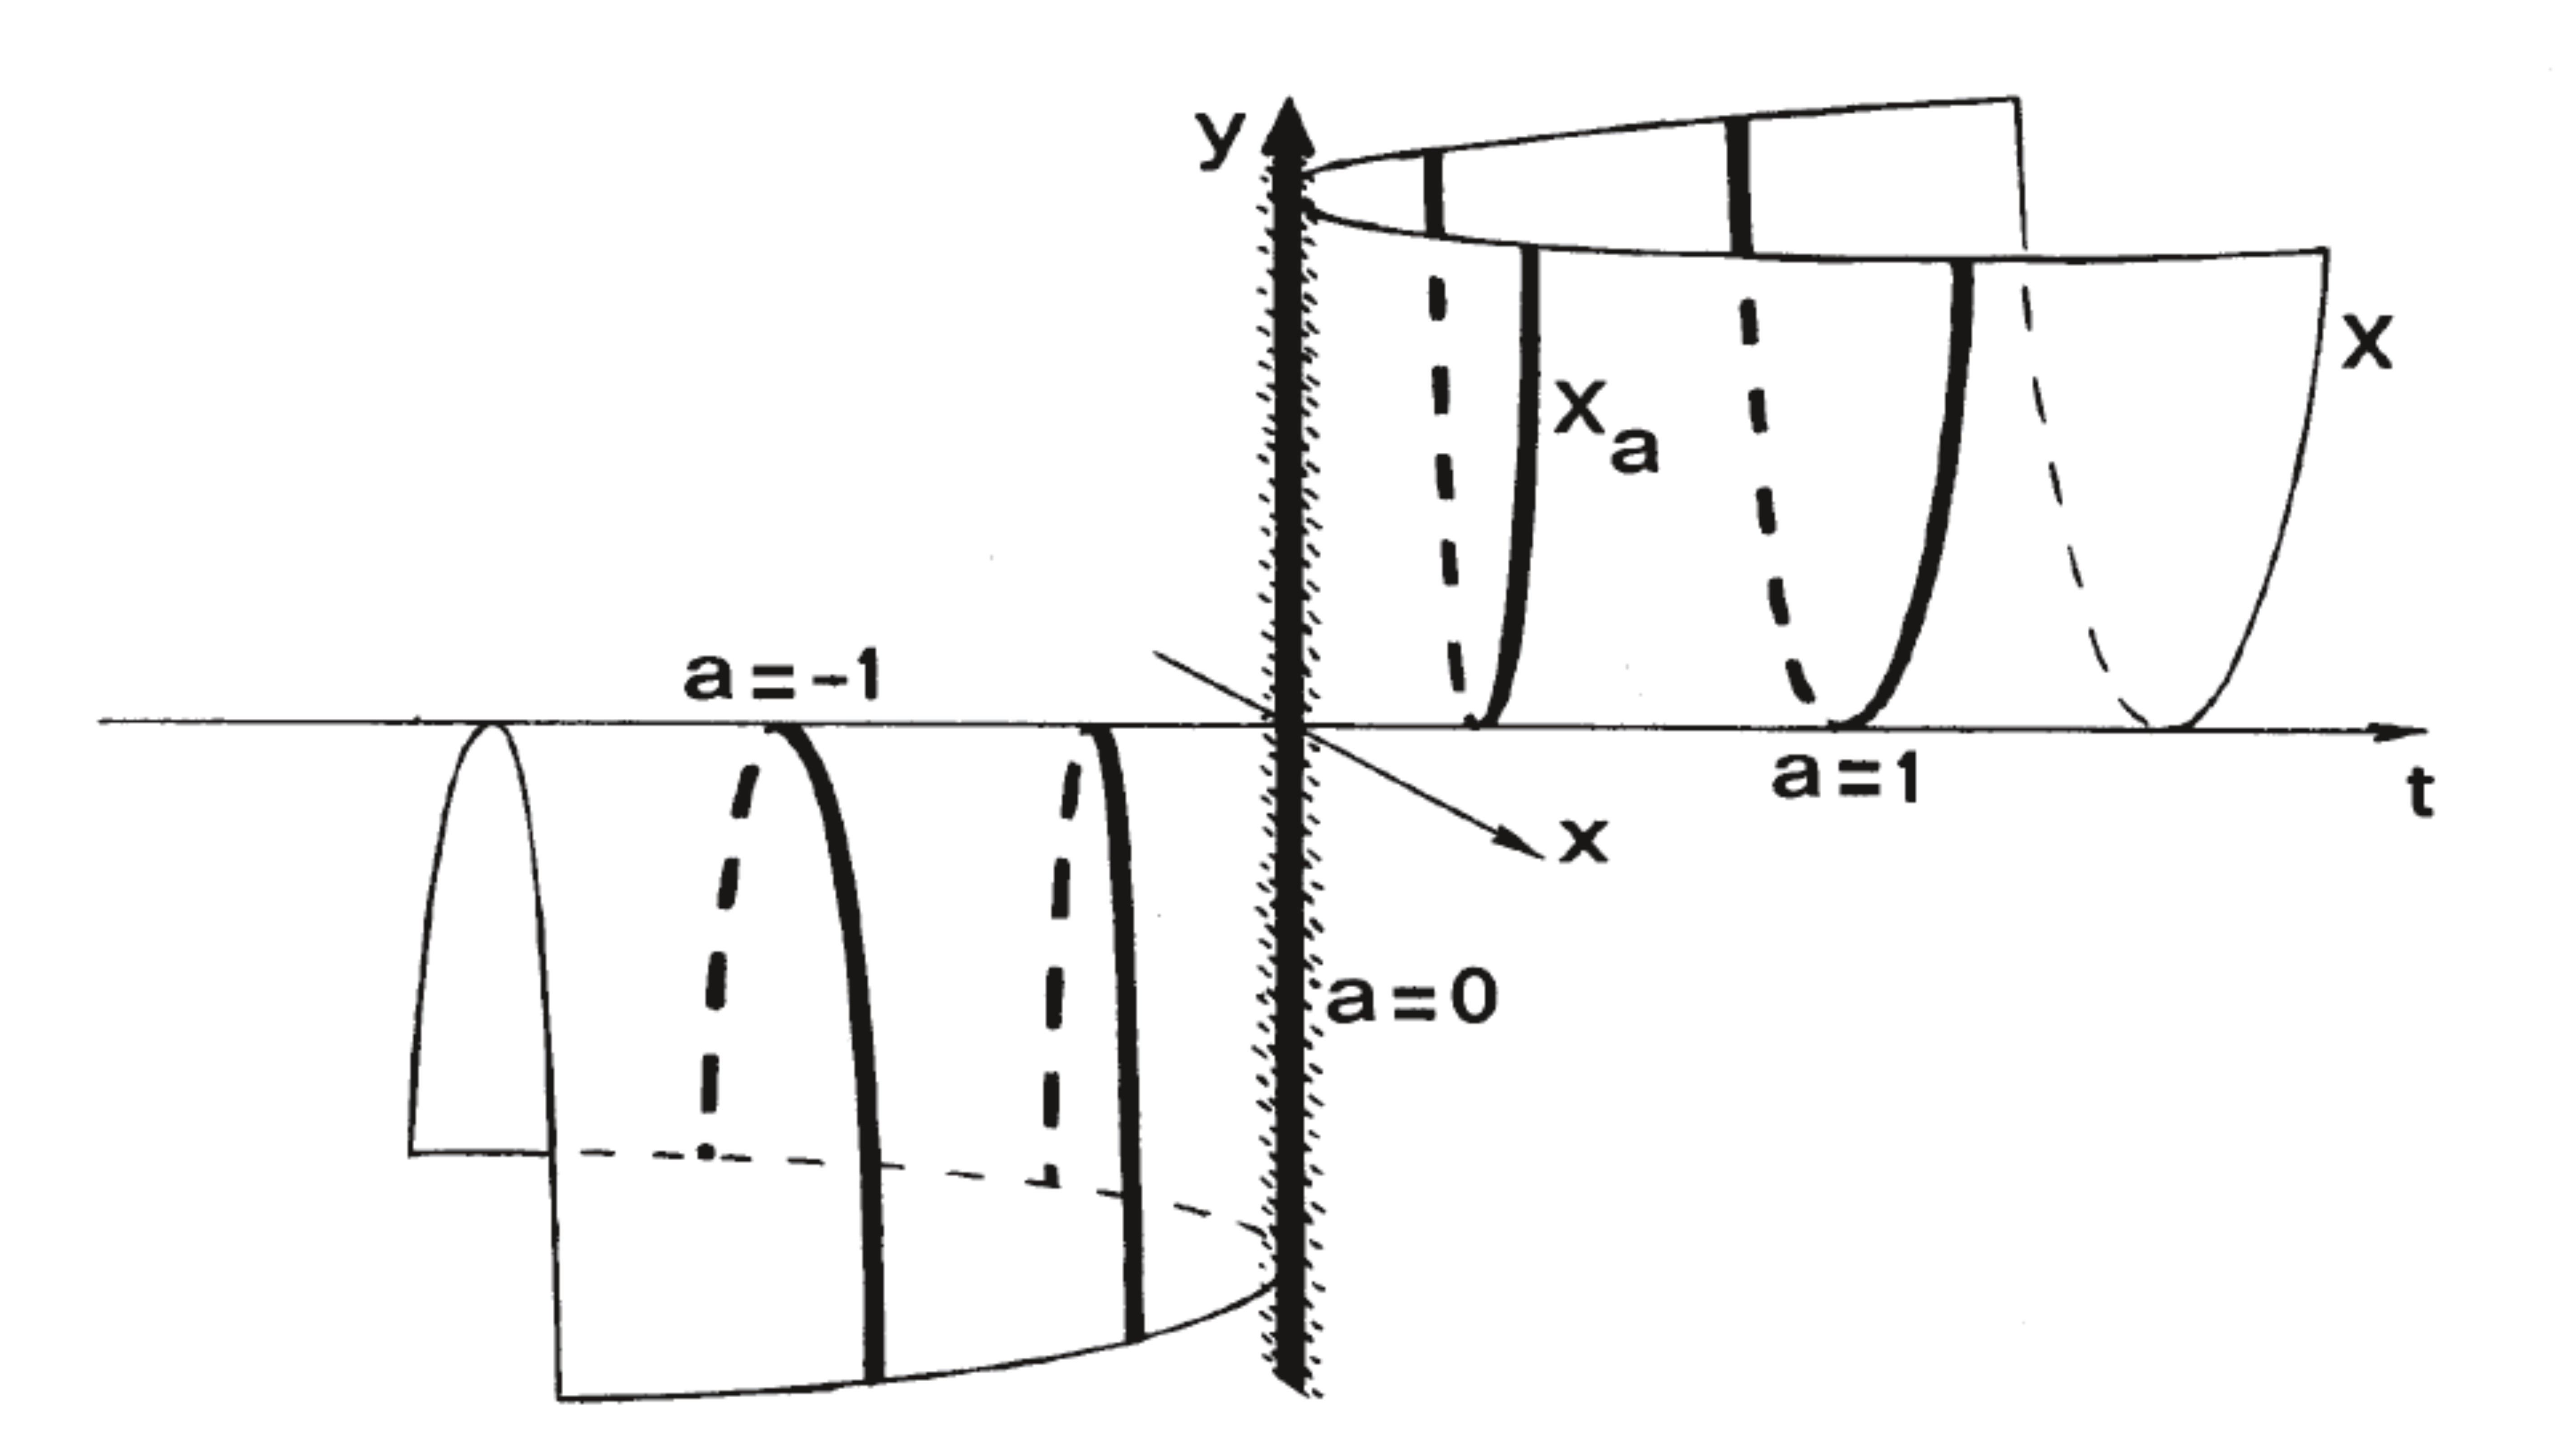
\includegraphics[width=10cm]{Figure7}\\
	Figure 7. 스킴들의 대수적 족
	\end{center}
	
	
	%Example 3.3.2
	\begin{example}
	%
		\tn{\\마찬가지로 만약 $X=\Spec k[x,y,t]/(xy-t)$이면 $a\ne 0$인 경우 일반적인 구성원 $X_a$는 기약 쌍곡선 $xy=a$이지만
		특수한 구성원 $X_0$는 두 직선으로 구성된 비기약 스킴 $xy=0$인 족을 얻는다.}
	%
	\end{example}
	
	
	
	%Exercises
	\subsection*{Exercises (연습문제)}
	
	\begin{enumerate}[label=\tb{3.\arabic*.},itemindent=0mm,itemsep=2mm]
	\item 사상 $f:X\ra Y$가 국소유한형일 필요충분조건은 $Y$의 \ti{모든} 아핀 열린 부분집합 $V=\Spec B$에 대하여
	$f^{-1}(V)$가 유한생성 $B$-대수 $A_j$들에 대한 아핀 열린 부분집합 $U_j=\Spec A_j$들로 덮일 수 있는 것이다.
	\item 스킴 사상 $f:X\ra Y$가 \tb{준컴팩트(quasi-compact)}라는 것의 정의는 아핀 열린집합 $V_i$들로 구성된
	$Y$의 덮개가 존재하여 각각의 $i$에 대하여 $f^{-1}(V_i)$가 준컴팩트한 것이다.
	$f$가 준컴팩트일 필요충분조건은 \ti{모든} 아핀 열린 부분집합 $V\bseq Y$에 대하여 $f^{-1}(V)$가 준컴팩트한 것임을 보여라.
	\item \begin{enumerate}[label=(\alph*)]
	\item 사상 $f:X\ra Y$가 유한형일 필요충분조건은 국소유한형이며 준컴팩트한 것이다.
	\item 이로부터 $f$가 유한형일 필요충분조건은 $Y$의 \ti{모든} 아핀 열린집합 $V=\Spec B$에 대하여
	$f^{-1}(V)$가 유한생성 $B$-대수 $A_j$들에 대한 유한 개 아핀 열린집합 $U_j=\Spec A_j$들로 덮일 수 있는 것이라 결론지어라.
	\item 만약 $f$가 유한형이면 \ti{모든} 아핀 열린 부분집합 $V=\Spec B\bseq Y$와
	\ti{모든} 아핀 열린집합 $U=\Spec A\bseq f^{-1}(V)$에 대하여 $A$가 유한생성 $B$-대수라는 사실도 보여라.
	\end{enumerate}
	\item 사상 $f:X\ra Y$가 유한일 필요충분조건은 $Y$의 \ti{모든} 아핀 열린 부분집합 $V=\Spec B$에 대하여
	$f^{-1}(V)$가 아핀이며 유한 $B$-모듈에 대한 $\Spec A$와 같은 것임을 보여라.
	\item 사상 $f:X\ra Y$가 \tb{준유한(quasi-finite)}이라는 것의 정의는 모든 점 $y\in Y$에 대하여 $f^{-1}(y)$가 유한집합인 것이다.
	\begin{enumerate}[label=(\alph*)]
	\item 유한 사상이 준유한임을 보여라.
	\item 유한 사상이 \ti{닫힌} 함수임을 보여라. i.e. 임의의 닫힌 부분집합의 상이 닫혀 있다.
	\item 전사 유한형 준유한 사상이 유한일 필요가 없음을 반례를 통해 보여라.
	\end{enumerate}
	\item $X$가 정수적 스킴이라 하자. $X$의 일반점 $\xi$의 국소환 $\mc O_\xi$가 체임을 보여라.
	이는 $X$의 \tb{함수체(function field)}라 불리며 $K(X)$로 표기된다.
	만약 $U=\Spec A$가 $X$의 임의의 아핀 열린 부분집합이면 $K(X)$는 $A$의 분수체와 동형이라는 사실도 보여라.
	\item $Y$가 기약인 경우 사상 $f:X\ra Y$가 \tb{일반유한(generically finite)}이라는 것의 정의는
	$Y$의 일반점 $\eta$에 대하여 $f^{-1}(\eta)$가 유한집합인 것이다.
	사상 $f:X\ra Y$가 \tb{우세(dominant)}라는 것의 정의는 $f(X)$가 $Y$에서 조밀한 것이다.
	이제 $f:X\ra Y$가 정수적 스킴 간의 우세 일반유한 유한형 사상이라 하자.
	조밀 열린 부분집합 $U\bseq Y$가 존재하여 유도된 사상 $f^{-1}(U)\ra U$가 유한이도록 함을 보여라.
	[Hint: 먼저 $X$의 함수체가 $Y$의 함수체의 유한 체 확대임을 보여라.]
	\item \tb{정규화.} 스킴이 \tb{정규(normal)}라는 것의 정의는 모든 국소환이 정수적으로 닫힌 정역인 것이다.
	$X$가 정수적 스킴이라 하자. $X$의 각각의 아핀 열린 부분집합 $U=\Spec A$에 대하여
	$\tilde A$가 $A$의 자신의 분수체에서의 정수적 폐포이며 $\tilde U=\Spec\tilde A$라 하자.
	스킴 $\tilde U$들을 붙이는 것으로 $X$의 \tb{정규화(normalization)}라 불리는 정규 정수적 스킴 $\tilde X$를 얻을 수 있음을 보여라.
	다음의 보편 성질을 가지는 사상 $\tilde X\ra X$가 존재한다는 사실도 보여라:
	모든 정규 정수적 스킴 $Z$와 모든 우세 사상 $f:Z\ra X$에 대하여 $f$는 $\tilde X$를 통해 유일하게 분해된다.
	만약 $X$가 $k$ 상에서 유한형이면 사상 $\tilde X\ra X$가 유한 사상이다. 이는 (I, Ex. 3.17)을 일반화한다.
	\item \tb{곱의 위상공간.} 대수다양체의 범주에서 두 대수다양체의 곱 상에서의 Zariski 위상이 곱위상과 같지 않았음을 상기하라.
	(I, Ex. 1.4) 이제 우리는 스킴의 범주에서 스킴의 곱의 기반 위상공간이 곱집합조차 아님을 보게 될 것이다.
	\begin{enumerate}[label=(\alph*)]
	\item $k$가 체이며 $\mb A^1_k=\Spec k[x]$가 $k$ 상에서의 아핀 직선이라 하자.
	$\mb A^1_k\times_{\Spec k}\mb A^1_k\cong\mb A^2_k$임을 보이고
	(심지어 $k$가 대수적으로 닫혀 있는 경우에도) 곱의 기반 점집합이 곱인자들의 기반 점집합의 곱집합이 아님을 보여라.
	\item $k$가 체이며 $s$와 $t$가 $k$ 상에서의 부정원이라 하자. 그 경우 $\Spec k(s),\Spec k(t)$와 $\Spec k$는 모두 한 점 공간이다.
	곱 스킴 $\Spec k(s)\times_{\Spec k}\Spec k(t)$를 기술하라.
	\end{enumerate}
	\item \tb{사상의 올.}
	\begin{enumerate}[label=(\alph*)]
	\item 만약 $f:X\ra Y$가 사상이며 $y\in Y$가 점이면 $\sp(X_y)$가 유도 위상을 가지는 $f^{-1}(y)$와 위상동형임을 보여라.
	\item $X=\Spec k[s,t]/(s-t^2)$이며 $Y=\Spec k[s]$이고 $f:X\ra Y$가 $s\mt s$에 의해 정의된 사상이라 하자.
	만약 $y\in Y$가 $a\ne 0$인 점 $a\in k$이면 올 $X_y$가 두 점으로 구성되며 잉여류체 $k$를 가짐을 보여라.
	만약 $y\in Y$가 $0\in k$에 대응되면 올 $X_y$가 비축약 한 점 스킴임을 보여라.
	만약 $\eta$가 $Y$의 일반점이면 $X_\eta$가 한 점 스킴이며 그 잉여류체가 $\eta$의 잉여류체의 차수 2의 확대체임을 보여라.
	($k$가 대수적으로 닫혀 있다 가정하라.)
	\end{enumerate}
	\item \tb{닫힌 부분스킴.}
	\begin{enumerate}[label=(\alph*)]
	\item 닫힌 몰입은 기반 확대 하에서 안정하다: 만약 $f:Y\ra X$가 닫힌 몰입이며 $X'\ra X$가 임의의 사상이면
	$f':Y\times_XX'\ra X'$도 닫힌 몰입이다.
	\end{enumerate}
	\begin{enumerate}[label=*(\alph*)]
	\setcounter{enumii}{1}
	\item 만약 $Y$가 아핀 스킴 $X=\Spec A$의 닫힌 부분스킴이면 $Y$도 아핀이다.
	사실 $Y$는 적절한 아이디얼 $\mf a\bseq A$에 의해 결정된 닫힌 몰입 $\Spec A/\mf a\ra\Spec A$의 상이다.
	[Hint: 먼저 $Y$가 $D(f_i)\cap Y\:(f_i\in A)$ 형태의 유한 개의 아핀 열린 부분집합들에 의해 덮일 수 있음을 보여라.
	필요하다면 $D(f_i)\cap Y=\es$인 $f_i$들을 추가하는 것으로 $D(f_i)$들이 $X$를 덮는다 가정할 수 있다.
	다음으로 $f_1,\ldots,f_r$이 $A$의 단위 아이디얼을 생성함을 보여라.
	그 후 (Ex. 2.17b)를 사용하여 $Y$가 아핀임을 보이고 (Ex. 2.18d)를 사용하여 $Y$가 아이디얼 $\mf a\bseq A$에 의해 결정됨을 보여라.]
	Note: 우리는 나중에 아이디얼의 층을 사용하여 이 결과의 다른 증명을 제시할 것이다. (5.10)
	\end{enumerate}
	\begin{enumerate}[label=(\alph*)]
	\setcounter{enumii}{2}
	\item $Y$가 스킴 $X$의 닫힌 부분집합이라 하고 $Y$에 축약 유도 부분스킴 구조를 부여하자.
	만약 $Y'$이 동일한 위상공간을 가지는 $X$의 임의의 다른 닫힌 부분스킴이면 닫힌 몰입 $Y\ra X$가 $Y'$을 통해 분해됨을 보여라.
	우리는 축약 유도 구조가 닫힌 부분집합 상에서의 최소 부분스킴 구조라 말하는 것으로 이러한 성질을 나타낸다.
	\item $f:Z\ra X$가 사상이라 하자. 그 경우 $X$의 유일한 닫힌 부분스킴 $Y$가 존재하여 다음 성질을 가진다:
	사상 $f$가 $Y$를 통해 분해되며, 만약 $Y'$이 $X$의 임의의 다른 닫힌 부분스킴이고 $f$가 $Y'$을 통해 분해된다면
	$Y\ra X$도 $Y'$을 통해 분해된다. 우리는 $Y$를 $f$의 \tb{스킴 이론적 상(scheme-theoretic image)}이라 한다.
	만약 $Z$가 축약 스킴이면 $Y$는 단지 상 $f(Z)$의 폐포 상에서의 축약 유도 구조이다.
	\end{enumerate}
	\item \tb{$\Proj S$의 닫힌 부분스킴.}
	\begin{enumerate}[label=(\alph*)]
	\item $\ph:S\ra T$가 등급을 보존하는 등급환 간의 전사 준동형사상이라 하자.
	(Ex. 2.14)의 열린집합 $U$가 $\Proj T$와 같으며 사상 $f:\Proj T\ra\Proj S$가 닫힌 몰입임을 보여라.
	\item 만약 $I\bseq S$가 동차 아이디얼이면 $T=S/I$라 하고 $Y$가 닫힌 몰입 $\Proj S/I\ra X$의 상으로 정의된
	$X=\Proj S$의 닫힌 부분스킴이라 하자. 서로 다른 동차 아이디얼들이 동일한 닫힌 부분스킴을 정의할 수 있음을 보여라.
	예를 들어 $d_0$가 정수라 하고 $I'=\bigoplus_{d\ge d_0}I_d$라 하자. $I$와 $I'$이 동일한 부분스킴을 결정함을 보여라.\\
	우리는 나중에 (5.16) (적어도 $S$가 $S_0$ 상에서의 다항식환인 경우)
	$X$의 모든 닫힌 부분스킴이 $S$의 동차 아이디얼 $I$에 의해 정의됨을 보일 것이다.
	\end{enumerate}
	\item \tb{유한형 사상의 성질.}
	\begin{enumerate}[label=(\alph*)]
	\item 닫힌 몰입은 유한형 사상이다.
	\item 준컴팩트 열린 몰입(Ex. 3.2)은 유한형이다.
	\item 두 유한형 사상의 합성은 유한형이다.
	\item 유한형 사상은 기반 확대 하에서 안정하다.
	\item 만약 $X$와 $Y$가 $S$ 상에서의 유한형 스킴이면 $X\times_SY$가 $S$ 상에서 유한형이다.
	\item 만약 $X\sr f\ra Y\sr g\ra Z$가 두 사상이며 $f$가 준컴팩트하고 $g\circ f$가 유한형이면 $f$가 유한형이다.
	\item 만약 $f:X\ra Y$가 유한형 사상이며 $Y$가 Noether이면 $X$가 Noether이다.
	\end{enumerate}
	\item 만약 $X$가 체 상에서의 유한형 스킴이면 $X$의 닫힌점들이 조밀함을 보여라.
	이것이 임의의 스킴에 대해서는 참이 아님을 반례를 통해 보여라.
	\item $X$가 (대수적으로 닫혀 있을 필요는 없는) 체 $k$ 상에서의 유한형 스킴이라 하자.
	\begin{enumerate}[label=(\alph*)]
	\item 다음 세 조건이 동치임을 보여라. (이 경우 우리는 $X$가 \tb{기하학적으로 기약(geometrically irreducible)}이라 한다.)\\[-2mm]
	\begin{enumerate}[label=(\roman*)]
	\item $X\times_k\bar k$가 기약이다. (여기에서 $\bar k$는 $k$의 대수적 폐포를 나타낸다.
	표기법의 남용으로 $X\times_{\Spec k}\Spec \bar k$를 $X\times_k\bar k$로 표기한다.)
	\item $X\times_kk_s$가 기약이다. (여기에서 $k_s$는 $k$의 가분 폐포를 나타낸다.)
	\item $k$의 모든 확대체 $K$에 대하여 $X\times_kK$가 기약이다.\\[-2mm]
	\end{enumerate}
	\item 다음 세 조건이 동치임을 보여라. (이 경우 우리는 $X$가 \tb{기하학적으로 축약(geometrically reduced)}이라 한다.)\\[-2mm]
	\begin{enumerate}[label=(\roman*)]
	\item $X\times_k\bar k$가 축약이다.
	\item $X\times_kk_p$가 축약이다. (여기에서 $k_p$는 $k$의 완전 폐포를 나타낸다.)
	\item $k$의 모든 확대체 $K$에 대하여 $X\times_kK$가 축약이다.\\[-2mm]
	\end{enumerate}
	\item 만약 $X\times_k\bar k$가 정수적이면 $X$가 \tb{기하학적으로 정수적(geometrically integral)}이라 한다.
	기하학적으로 기약이 아니며 기하학적으로 축약이 아닌 정수적 스킴의 예를 제시하라.
	\end{enumerate}
	\item \tb{Noether 귀납법.} $X$가 Noether 위상공간이며 $\ms P$가 $X$의 닫힌 부분집합들의 성질이라 하자.
	$X$의 임의의 닫힌 부분집합 $Y$에 대하여 만약 $\ms P$가 $Y$의 모든 닫힌 진부분집합에 대하여 성립한다면
	$\ms P$가 $Y$에 대하여 성립한다 하자. (특히 $\ms P$는 공집합에 대하여 반드시 성립해야 한다.)
	그 경우 $\ms P$가 $X$에 대하여 성립한다.
	\item \tb{Zariski 공간.} 위상공간 $X$가 \tb{Zariski 공간(Zariski space)}이라는 것의 정의는 Noether이며
	모든 (공집합이 아닌) 기약 닫힌집합이 유일한 일반점을 가지는 것이다. (Ex. 2.9)\\
	예를 들어 $R$이 이산 부치환이며 $T=\sp(\Spec R)$이라 하자. 그 경우 $T$는 두 점 $t_0=$극대 아이디얼, $t_1=0$ 아이디얼로 구성된다.
	열린 부분집합은 $\es,\{t_1\},T$이다. 이는 일반점 $t_1$을 가지는 기약 Zariski 공간이다.
	\begin{enumerate}[label=(\alph*)]
	\item 만약 $X$가 Noether 스킴이면 $\sp(X)$가 Zariski 공간임을 보여라.
	\item Zariski 공간의 임의의 극소 공집합이 아닌 닫힌 부분집합은 한 점으로 구성된다.
	우리는 이들을 \tb{닫힌점(closed point)}이라 부른다.
	\item Zariski 공간 $X$가 $T_0$ 공리를 만족시킴을 보여라:
	$X$의 주어진 서로 다른 임의의 두 점에 대하여 이들 중 정확히 하나만을 포함하는 열린집합이 존재한다.
	\item 만약 $X$가 기약 Zariski 공간이면 그 일반점은 $X$의 모든 공집합이 아닌 열린 부분집합에 포함된다.
	\item 만약 $x_0,x_1$이 위상공간 $X$의 점이며 $x_0\in\overline{\{x_1\}}$이면
	우리는 $x_1$이 $x_0$에 \tb{특수화(specialize)}된다고 하며 $x_1\rightsquigarrow x_0$로 표기한다.
	또한 우리는 $x_0$가 $x_1$의 \tb{특수화(specialization)}이며 $x_1$이 $x_0$의 \tb{일반화(generalization)}라 한다.
	이제 $X$가 Zariski 공간이라 하자. $x_1\rightsquigarrow x_0$이면 $x_1>x_0$이도록 결정된 부분순서 하에서의 극소원들이 닫힌점들이며
	극대원들이 $X$의 기약 성분의 일반점들임을 보여라. 닫힌집합이 자신의 임의의 점의 모든 특수화를 포함함을 보여라.
	(우리는 닫힌집합들이 \tb{특수화 하에서 안정(stable under specialization)}하다고 한다.)
	마찬가지로 열린 부분집합들은 \tb{일반화 하에서 안정(stable under generalization)}하다.
	\item $t$가 (2.6)의 증명에서 도입된 위상공간들 상에서의 함자라 하자.
	만약 $X$가 Noether 위상공간이면 $t(X)$가 Zariski 공간임을 보여라.
	이에 더해 $X$ 자신이 Zariski 공간일 필요충분조건은 함수 $X\ra t(X)$가 위상동형사상인 것이다.
	\end{enumerate}
	\item \tb{구축 가능 집합.} $X$가 Zariski 위상공간이라 하자. $X$의 \tb{구축 가능 부분집합(constructible subset)}은
	(1) 모든 열린집합이 $\mf F$에 속하고 (2) $\mf F$의 원소들의 유한 교집합이 $\mf F$에 속하고
	(3) $\mf F$의 원소의 여집합이 $\mf F$에 속하도록 하는 부분집합들의 최소 집합족 $\mf F$의 원소이다.
	\begin{enumerate}[label=(\alph*)]
	\item $X$의 부분집합이 \tb{국소 닫혀 있다(locally closed)}는 것의 정의는 열린 부분집합과 닫힌 부분집합의 교집합인 것이다.
	$X$의 부분집합이 구축 가능할 필요충분조건은 국소 닫힌집합들의 유한 분리합집합으로 표현 가능한 것임을 보여라.
	\item 기약 Zariski 공간 $X$의 구축 가능 부분집합이 조밀할 필요충분조건은 일반점을 포함하는 것임을 보여라.
	이에 더해 그 경우 이는 공집합이 아닌 열린 부분집합을 포함한다.
	\item $X$의 부분집합 $S$가 닫혀 있을 필요충분조건은 구축 가능하며 특수화 하에서 안정한 것이다.
	마찬가지로 $X$의 부분집합 $T$가 열려 있을 필요충분조건은 구축 가능하며 일반화 하에서 안정한 것이다.
	\item 만약 $f:X\ra Y$가 Zariski 공간 간의 연속 함수이면 $Y$의 임의의 구축 가능 부분집합의 역상은 $X$의 구축 가능 부분집합이다.
	\end{enumerate}
	\item 구축 가능 부분집합의 개념의 진정한 중요성은 Chevalley에 의한 다음의 정리에서 따라온다 - 
	Cartan and Chevalley [1, expos\'e 7]과 Matsumura [2, Ch. 2 \S 6]을 참조하라:
	$f:X\ra Y$가 Noether 스킴의 유한형 사상이라 하자. 그 경우 $X$의 임의의 구축 가능 부분집합의 상은 $Y$의 구축 가능 부분집합이다.
	특히 $f(X)$는 (열린집합이거나 닫힌집합일 필요는 없지만) $Y$의 구축 가능 부분집합이다. 이 정리를 다음 단계를 통해 증명하라.
	\begin{enumerate}[label=(\alph*)]
	\item $X$와 $Y$가 아핀 정수적 Noether 스킴이며 $f$가 우세 사상인 경우 $f(X)$ 자신이 구축 가능함을 보이는 것으로 문제를 줄여라.
	\end{enumerate}
	\begin{enumerate}[label=*(\alph*)]
	\setcounter{enumii}{1}
	\item 그 경우 다음의 가환대수학의 결과를 이용하여 $f(X)$가 $Y$의 공집합이 아닌 열린 부분집합을 포함함을 보여라:
	$A\bseq B$가 Noether 정역의 포함 관계이며 $B$가 유한생성 $A$-대수라 하자.
	0이 아닌 원소 $b\in B$가 주어진 경우 0이 아닌 원소 $a\in A$가 존재하여 다음 성질을 가진다:
	만약 $\ph:A\ra K$가 $A$에서 대수적으로 닫힌 체 $K$로의 임의의 준동형사상이며 $\ph(a)\ne 0$을 만족시키면
	$\ph$는 $\ph'(b)\ne 0$을 만족시키는 $B$에서 $K$로의 준동형사상 $\ph'$으로 확장된다.
	[Hint: 이러한 대수학적 결과를 $B$의 $A$ 상에서의 생성자의 개수에 대한 귀납법을 통해 보여라.
	1개 생성자의 경우 결과를 직접적으로 증명하라. $b=1$인 경우에 대하여 적용하라.]
	\end{enumerate}
	\begin{enumerate}[label=(\alph*)]
	\setcounter{enumii}{2}
	\item 이제 $Y$에 대한 Noether 귀납법을 사용하여 증명을 완료하라.
	\item $f(X)$가 열린집합도 닫힌집합도 아니도록 하는 대수적으로 닫힌 체 $k$ 상에서의 대수다양체 간의 사상 $f:X\ra Y$의 예를 제시하라.
	\end{enumerate}
	\item \tb{차원.} $X$가 (대수적으로 닫혀 있을 필요는 없는) 체 $k$ 상에서의 유한형 정수적 스킴이라 하자.
	(I, \S 1)에서의 적절한 결과들을 사용하여 다음을 증명하라.
	\begin{enumerate}[label=(\alph*)]
	\item 임의의 닫힌점 $P\in X$에 대하여 $\dim X=\dim\mc O_P$이다. (환의 차원은 항상 Krull 차원을 의미한다.)
	\item $K(X)$가 $X$의 함수체라 하자. (Ex. 3.6) 그 경우 $\dim X=\trd K(X)/k$이다.
	\item 만약 $Y$가 $X$의 닫힌 부분집합이면 $\codim(Y,X)=\inf\sx{\dim\mc O_{P,X}}{P\in Y}$이다.
	\item 만약 $Y$가 $X$의 닫힌 부분집합이면 $\dim Y+\codim(Y,X)=\dim X$이다.
	\item 만약 $U$가 $X$의 공집합이 아닌 열린 부분집합이면 $\dim U=\dim X$이다.
	\item 만약 $k\bseq k'$이 체 확대이면 $X'=X\times_kk'$의 모든 기약 성분이 차원 $\dim X$를 가진다.
	\end{enumerate}
	\item $R$이 자신의 잉여류체 $k$를 포함하는 이산 부치환이라 하자. $X=\Spec R[t]$가 $\Spec R$ 상에서의 아핀 직선이라 하자.
	(Ex. 3.20)의 진술 (a), (d), (e)가 $X$에 대하여 거짓임을 보여라.\\[-2.3mm]
	\end{enumerate}
	\begin{enumerate}[label=\tb{*3.\arabic*.},itemindent=0mm,itemsep=2mm]
	\setcounter{enumi}{21}
	\item \tb{사상의 올의 차원.} $f:X\ra Y$가 $k$ 상에서의 유한형 정수적 스킴 간의 우세 사상이라 하자.
	\begin{enumerate}[label=(\alph*)]
	\item $Y'$이 $Y$의 닫힌 기약 부분집합이며 그 일반점 $\eta'$이 $f(X)$에 포함되어 있다 하자.
	$Z$가 $\eta'\in f(Z)$를 만족시키는 $f^{-1}(Y')$의 임의의 기약 성분이라 하자. $\codim(Z,X)\le\codim(Y',Y)$임을 보여라.
	\item $e=\dim X-\dim Y$가 $X$의 $Y$ 상에서의 \tb{상대적 차원(relative dimension)}이라 하자.
	임의의 점 $y\in f(X)$에 대하여 올 $X_y$의 모든 기약 성분이 차원 $e$ 이상임을 보여라.
	[Hint: $Y'=\overline{\{y\}}$라 하고 (Ex. 3.20b)와 (a)를 사용하라.]
	\item 조밀 열린 부분집합 $U\bseq X$가 존재하여 임의의 $y\in f(U)$에 대하여 $\dim U_y=e$를 만족시킴을 보여라.
	[Hint: 먼저 $X$와 $Y$가 아핀인 경우로 문제를 줄여라. $X=\Spec A,Y=\Spec B$라 하자. 그 경우 $A$는 유한생성 $B$-대수이다.
	$t_1,\ldots,t_e\in A$가 $K(X)$의 $K(Y)$ 상에서의 초월 기저라 하고 $X_1=\Spec B[t_1,\ldots,t_e]$라 하자.
	그 경우 $X_1$이 $Y$ 상에서의 아핀 $e$-공간과 동형이며 사상 $X\ra X_1$이 일반유한이다. 이제 위의 (Ex. 3.7)을 사용하라.]
	\item 원래 사상 $f:X\ra Y$로 되돌아가 임의의 정수 $h$에 대하여 $E_h$가 다음을 만족시키는 점 $x\in X$들의 집합이라 하자:
	$y=f(x)$라 하면 올 $X_y$의 기약 성분 $Z$가 존재하여 $x\in Z$이며 $\dim Z\ge h$이다.
	(1) $E_e=X$이며 (위의 (b)를 사용하라) (2) 만약 $h>e$이면 $E_h$가 $X$에서 조밀하지 않고 (위의 (c)를 사용하라)
	(3) 모든 $h$에 대하여 $E_h$가 닫혀 있다. ($\dim X$에 대한 귀납법을 사용하라.)
	\item Chevalley에 의한 다음 정리를 증명하라 - Cartan and Chevalley [1, expos\'e 8]을 참조하라.
	각각의 정수 $h$에 대하여 $C_h$가 $\dim X_y=h$를 만족시키는 점 $y\in Y$들의 집합이라 하자.
	그 경우 부분집합 $C_h$들은 구축 가능하며 $C_e$가 $Y$의 조밀 열린 부분집합을 포함한다.\\[-2.3mm]
	\end{enumerate}
	\end{enumerate}
	\begin{enumerate}[label=\tb{3.\arabic*.},itemindent=0mm,itemsep=2mm]
	\setcounter{enumi}{22}
	\item 만약 $V,W$가 대수적으로 닫힌 체 $k$ 상에서의 두 대수다양체이고 $V\times W$가
	(I, Ex. 3.15, 3.16)에서 정의된 이들의 곱이며 $t$가 (2.6)의 함자이면 $t(V\times W)=t(V)\times_{\Spec k}t(W)$이다.
	\end{enumerate}
	
	
	
	%Section 4
	\section{Separated and Proper Morphism (분리 및 진 사상)}
	
	이제 우리는 통상적인 위상공간의 잘 알려진 성질에 대응하는 스킴, 또는 스킴 간의 사상의 두 가지 성질을 다룰 것이다.
	분리성은 위상공간에 대한 Hausdorff 공리에 대응한다.
	진성은 통상적인 진성의 개념, 즉 컴팩트 부분집합의 역사이 컴팩트라는 것에 대응한다.
	그러나 Zariski 위상은 절대 Hausdorff가 아니며 스킴의 기반위상공간이 스킴의 모든 성질을 정확히 반영하지 않으므로
	통상적인 정의는 추상적 대수기하학에서 적절하지 않다.
	그러므로 우리는 대신 스킴의 범주 내에서 사상의 함자적 거동을 반영하는 정의를 사용할 것이다.
	$\C$ 상에서의 유한형 스킴들에 대하여 우리는 추상적으로 정의된 이러한 개념들이 사실은
	이러한 스킴들을 통상적인 위상을 가지는 복소해석학적 공간으로 간주했을 경우의 통상적인 개념들과 같음을 보일 수 있다. (Appendix B)
	
	이 절에서 우리는 분리 사상과 진 사상을 정의할 것이다.
	우리는 사상이 분리 사상 또는 진 사상인지에 대한 부치환을 이용한 판정법을 제시할 것이다.
	그 후 우리는 임의의 스킴 상에서의 사영 스킴이 진 스킴임을 보일 것이다.
	
	
	%Definition
	\begin{definition}
	%
		\tn{$f:X\ra Y$가 스킴 사상이라 하자. \tb{대각사상(diagonal morphism)}은 두 사영사상 $p_1,p_2:X\times_YX\ra X$와의 합성이
		항등사상 $X\ra X$이도록 하는 유일한 사상 $\De:X\ra X\times_YX$이다.
		사상 $f$가 \tb{분리(separated)}라는 것의 정의는 대각사상 $\De$가 닫힌 몰입인 것이다.
		이 경우 우리는 \tb{$X$가 $Y$ 상에서 분리($X$ is separated over $Y$)}라고 한다.
		스킴 $X$가 \tb{분리(separated)}라는 것의 정의는 $\Spec\Z$ 상에서 분리인 것이다.}
	%
	\end{definition}
	
	
	%Example 4.0.1
	\begin{example}
	%
		\tn{\\$k$가 체이며 $X$가 원점이 2개인 아핀 직선이라 하자. (2.3.6) 그 경우 $X$는 $k$ 상에서 분리가 아니다:
		$X\times_kX$는 각각의 축이 2개씩이고 원점이 4개인 아핀 평면이다. $\De$의 상은 원점이 2개인 대각선이다.
		4개의 원점이 모두 $\De(X)$의 폐포에 속하므로 이는 닫힌집합이 아니다.}
	%
	\end{example}
	
	
	%Example 4.0.2
	\begin{example}
	%
		\tn{\\우리는 나중에 (4.10) 만약 $C$가 대수적으로 닫힌 체 $k$ 상에서의 임의의 대수다양체이면
		연관된 스킴 $t(V)$가 $k$ 상에서 분리임을 보일 것이다.}
	%
	\end{example}
	
	
	%Proposition 4.1
	\begin{proposition}
	%
		\tn{만약 $f:X\ra Y$가 아핀 스킴 간의 임의의 사상이면 $f$가 분리이다.\\\\
	%
		\pf $X=\Spec A,Y=\Spec B$라 하자. 그 경우 $A$는 $B$-대수이며 $X\times_YX$는 $\Spec A\otimes_BA$로 주어지는 아핀 스킴이다.
		대각 사상 $\De$는 $a\otimes a'\ra aa'$으로 정의된 \tb{대각 준동형사상(diagonal homomorphism)}
		$A\otimes_BA\ra A$에 의해 주어진다. 이는 전사 환 준동형사상이며 따라서 $\De$는 닫힌 몰입이다.}
	%
		\qed
	%
	\end{proposition}
	
	
	%Corollary 4.2
	\begin{corollary}
	%
		\tn{\\임의의 사상 $f:X\ra Y$가 분리일 필요충분조건은 대각 사상의 상이 $X\times_YX$의 닫힌 부분집합인 것이다.\\\\
	%
		\pf 한쪽 방향은 자명하다. 그러므로 $\De(X)$가 닫힌 부분집합이면 $\De:X\ra X\times_YX$가 닫힌 몰입임을 증명하면 충분하다.
		다르게 표현하면 우리는 $\De:X\ra\De(X)$가 위상동형사상이며
		층의 사상 $\mc O_{X\times_YX}\ra\De_*\mc O_X$가 전사임을 확인해야 한다. $p_1:X\times_YX\ra X$가 첫째 사영이라 하자.
		$p_1\circ\De=\id_X$이므로 $\De$가 $\De(X)$로의 위상동형사상을 제공함이 즉시 따라온다.
		층의 사상 $\mc O_{X\times_YX}\ra\De_*\mc O_X$가 전사임을 보이는 것은 국소적인 문제이다.
		임의의 점 $P\in X$에 대하여 $U$가 다음을 만족시키는 $P$의 충분히 작은 아핀 열린 근방이라 하자:
		$f(U)$가 $Y$의 아핀 열린 부분집합 $V$에 포함된다.
		그 경우 $U\times_VU$는 $\De(P)$의 아핀 열린 근방이며, 위 명제에 의해 $\De:U\ra U\times_VU$가 닫힌 몰입이다.
		그러므로 우리의 층의 사상은 $P$의 근방에서 전사이며 이는 증명을 완료한다.}
	%
		\qed
	%
	\end{corollary}
	
	다음으로 우리는 분리성의 부치 판정법을 논할 것이다.
	개략적인 발상은 스킴 $X$가 분리이기 위해서는 위 예와 같이 2배 점을 포함하는 곡선처럼 보이는 부분스킴을 갖지 않아야 한다는 것이다.
	이를 표현하는 다른 방법은 만약 $C$가 곡선이며 $P$가 $C$의 점이면 임의의 주어진 사상 $C-P\ra X$가
	사상 $C\ra X$로의 확장을 하나 이하로 가져야 한다는 것이다.
	(사영 대수다양체가 이러한 성질을 가짐을 보였던 (I, 6.8)과 비교해 보라.)
	
	사실 이러한 대략적인 발상은 변형되어야 한다.
	국소적인 문제를 다루므로 우리는 곡선을 그 $P$에서의 국소환으로 대체할 수 있으며 이는 이산 부치환이다.
	우리가 다루는 스킴이 상당히 일반적일 것이므로 우리는 임의의 (이산이 아닐 수 있는) 부치환을 고려해야 한다.
	마지막으로 우리는 사상의 상 스킴 $Y$ 상에서 상대적인 판정법을 만들어야 한다.
	
	부치환의 정의와 기본 성질에 대해서는 (I, \S 6)을 참조하라.
	
	
	%Theorem 4.3
	\begin{theorem}[Valuative Criterion of Separatedness (분리성의 부치 판정법)]
	%
		\tn{\\$f:X\ra Y$가 스킴 사상이며 $X$가 Noether라 하자. 그 경우 $f$가 분리일 필요충분조건은 다음의 조건이 성립하는 것이다:
		임의의 체 $K$와 분수체가 $K$인 임의의 부치환 $R$에 대하여 $T=\Spec R,U=\Spec K$이며
		$i:U\ra T$가 포함 준동형사상 $R\bseq K$에 의해 유도된 사상이라 하자.
		다음의 가환 도표를 만족시키는 주어진 사상 $T\ra Y$와 $U\ra X$에 대하여
		하나 이하의 사상 $T\ra X$가 존재하여 전체 도표가 가환이도록 한다.}
	%
		$$\begin{tikzcd}[column sep=2cm]U\arrow[r]\arrow[d,swap,"i"]&X\arrow[d,"f"]\\
		T\arrow[r]\arrow[ur,dashed]&Y\end{tikzcd}$$
	%
	\end{theorem}
	
	두 가지 보조정리가 필요하다.
	
	
	%Lemma 4.4
	\begin{lemma}
	%
		\tn{\\$R$이 체 $K$의 부치환이라 하자. $T=\Spec R,U=\Spec K$라 하자.
		$U$에서 스킴 $X$로의 사상을 제시하는 것은 점 $x_1\in X$와 체의 포함 관계 $k(x_1)\bseq K$를 제시하는 것과 동치이다.
		$T$에서 $X$로의 사상을 제시하는 것은 $x_0$가 $x_1$의 특수화(Ex. 3.17e)이도록 하는 두 점 $x_0,x_1\in X$와
		다음을 만족시키는 체의 포함 관계 $k(x_1)\bseq K$를 제시하는 것과 같다:
		축약 유도 구조를 가지는 $X$의 부분스킴 $Z=\overline{x_1}$ 상에서의 $x_0$의 부치환이 $R$에 의해 지배된다.\\\\
	%
		\pf $U$는 한 점 스킴이며 구조층 $K$를 가진다. 국소준동형사상 $\mc O_{x,X}\ra K$를 제시하는 것은
		$k(x_1)\bseq K$를 제시하는 것과 같으므로 전반부는 자명하다.
		후반부를 보이기 위해 $t_0=\mf m_R$이 $T$의 닫힌점이며 $t_1=(0)$이 $T$의 일반점이라 하자.
		사상 $T\ra X$가 주어진 경우 $x_0$과 $x_1$을 $t_0$과 $t_1$의 상이라 하자.
		$T$가 축약이므로 사상 $T\ra X$는 $Z$를 통해 분해된다. (Ex. 3.11) 이에 더해 $k(x_1)$은 $Z$의 함수체이다.
		그러므로 우리는 포함 관계 $k(x_1)\bseq K$와 호환되는 $\mc O=\mc O_{x_0,Z}$에서 $R$로의 국소준동형사상을 얻는다.
		다르게 표현하면 $R$이 $\mc O$를 지배한다.\\
		역으로 $x_0,x_1$과 $R$이 $\mc O$를 지배하도록 하는 포함 관계 $k(x_1)\bseq K$로 구성된 데이터가 주어진 경우
		포함 준동형사상 $\mc O\ra R$은 사상 $T\ra\Spec\mc O$를 제공한다.
		이를 자연스러운 사상 $\Spec\mc O\ra X$와 합성하면 요구된 사상 $T\ra X$를 얻는다.}
	%
		\qed
	%
	\end{lemma}
	
	
	%Lemma 4.5
	\begin{lemma}
	%
		\tn{\\$f:X\ra Y$가 준컴팩트 스킴 사상이라 하자. (Ex. 3.2)
		그 경우 $Y$의 부분집합 $f(X)$가 닫힌집합일 필요충분조건은 특수화 하에서 안정한 것이다. (Ex. 3.17e)\\\\
	%
		\pf 한쪽 포함 관계는 자명하므로 우리는 만약 $f(X)$가 특수화 하에서 안정하면 닫혀 있음을 보이면 충분하다.
		우리는 명백히 $X$와 $Y$가 모두 축약이며 $\overline{f(X)}=Y$라 가정할 수 있다.
		($Y$를 $\overline{f(X)}$ 상에서의 축약 유도 구조로 대체하라.) 이제 $y\in Y$가 점이라 하자. $y\in f(X)$임을 보여야 한다.
		이제 우리는 $Y$를 $y$의 아핀 근방으로 대체할 수 있으며 따라서 $Y$가 아핀이라 가정할 것이다.
		$f$가 준컴팩트이므로 $X$는 아핀 열린집합 $X_i$들의 유한 합집합이다. 우리는 $y\in\overline{f(X)}$임을 알고 있다.
		그러므로 어떠한 $i$에 대하여 $y\in\overline{f(X_i)}$이다. $Y_i=\overline{f(X_i)}$가 축약 유도 구조를 가진다 하자.
		그 경우 $Y_i$도 아핀이며 우리는 축약 아핀 스킴 간의 우세 사상 $X_i\ra Y_i$를 고려할 것이다.
		$X_i=\Spec A$이며 $Y_i=\Spec B$라 하자. 그 경우 사상이 우세이므로 대응하는 환 준동형사상 $B\ra A$가 단사이다.
		점 $y\in Y_i$는 소 아이디얼 $\mf p\bseq B$에 대응한다. $\mf p'\bseq\mf p$가 $\mf p$에 포함된 $B$의 극소 아이디얼이라 하자.
		(포함 관계에 의해 전순서화된 소 아이디얼들의 임의의 족의 교집합이 소 아이디얼이 되므로
		Zorn 보조정리에 의해 극소 소 아이디얼이 존재한다.)
		그 경우 $\mf p'$은 $y$로 특수화되는 점 $y'\in Y_i$에 대응된다. $y'\in f(X_i)$임을 주장하겠다:
		$A$와 $B$를 $\mf p'$에서 국소화하자. 국소화가 완전 함자이므로 $B_{\mf p'}\bseq A\otimes B_{\mf p'}$이다.
		이제 $B_{\mf p'}$은 체이다. $\mf q_0'$이 $A\otimes B_{\mf p'}$의 임의의 소 아이디얼이라 하자.
		그 경우 $\mf q_0'\cap B_{\mf p'}=(0)$이다.
		$\mf q'\bseq A$가 $\mf q_0'$의 국소화 준동형사상 $A\ra A\otimes B_{\mf p'}$ 하에서의 역상이라 하자.
		그 경우 $\mf q'\cap B=\mf p'$이다. 그러므로 $\mf q'$은 $f(x')=y'$인 점 $x'\in X_i$에 대응한다.
		이제 사상 $f:X\ra Y$로 되돌아가자. $x'\in X,f(x')=y'$을 얻었으므로 $y'\in f(X)$이다. 이는 증명을 완료한다.}
	%
		\qed
	%
	\end{lemma}
	%
	\noindent\tb{Proof of Theorem 4.3.} 먼저 $f$가 분리이고 위에서와 같은 가환 도표가 주어졌으며
	두 사상 $h,h':T\ra X$가 전체 도표가 가환이도록 한다고 가정하자.
	%
	$$\begin{tikzcd}[column sep=2cm]U\arrow[r]\arrow[d,swap,"i"]&X\arrow[d,"f"]\\
	T\arrow[ur,"h'",swap,shift right]\arrow[ur,"h",shift left]\arrow[r]&Y\end{tikzcd}$$
	%
	그 경우 우리는 사상 $h'':T\ra X\times_YX$를 얻는다.
	$h$와 $h'$의 $U$로의 제한이 동일하므로 $T$의 일반점 $t_1$의 상은 대각 $\De(X)$에 속한다.
	$\De(X)$가 닫혀 있으므로 $t_0$의 상도 대각에 속한다.
	그러므로 $h$와 $h'$은 점 $t_0,t_1$을 $X$의 동일한 점 $x_0,x_1$로 대응시키며 따라서 (4.4)에 의해 $h$와 $h'$이 일치한다.\\
	역으로 정리의 조건이 만족되었다 가정하자.
	(4.2)에 의해 $f$가 분리임을 보이기 위해서는 $\De(X)$가 $X\times_YX$의 닫힌 부분집합임을 보이면 충분하다.
	$X$가 Noether라 가정했으므로 사상 $\De$가 준컴팩트이며 따라서 (4.5)에 의해 $\De(X)$가 특수화 하에서 안정함을 보이면 충분하다.
	그러므로 $\xi_1\in\De(X)$가 점이며 $\xi_1\rightsquigarrow\xi_0$가 특수화라 하자.
	$K=k(\xi_1)$이며 $\mc O$가 축약 유도 구조를 가지는 부분스킴 $\overline{\{\xi_1\}}$ 상에서의 $\xi_0$의 국소환이라 하자.
	그 경우 $\mc O$는 $K$에 포함된 국소환이며 따라서 (I, 6.1A)에 의해 $K$의 부치환 $R$이 존재하여 $\mc O$를 지배한다.
	(4.4)에 의해 우리는 $t_0$과 $t_1$을 $\xi_0$과 $\xi_1$로 대응시키는 $T=\Spec R$에서 $X\times_YX$로의 사상을 얻는다.
	사영 $p_1,p_2$와의 합성은 $T$에서 $X$로의 2개의 사상을 주며 이들은 동일한 $Y$로의 사상을 제공하고
	($\xi_1\in\De(X)$이므로) $U=\Spec K$로의 제한이 일치한다. 따라서 조건에 의해 두 사상 $T\ra X$가 일치해야 한다.
	그러므로 사상 $T\ra X\times_YX$가 대각 사상 $\De:X\ra X\times_YX$를 통해 분해되며 따라서 $\xi_0\in\De(X)$이다.
	이는 증명을 완료한다. 마지막 단계에서 $p_1(\xi_0)=p_2(\xi_0)$이라는 사실을 아는 것만으로는 부족함을 기억해 두라.
	일반적으로 만약 $\xi\in X\times_YX$이면 $p_1(\xi)=p_2(\xi)$가 $\xi\in\De(X)$를 함의하지 \ti{않는다}.
	
	
	%Corollary 4.6
	\begin{corollary}
	%
		\tn{\\다음 진술의 모든 스킴이 Noether라 가정하라.\\[-2mm]
	%
		\begin{enumerate}[label=(\alph*)]
		\item 열린 및 닫힌 몰입은 분리이다.
		\item 두 분리 사상의 합성은 분리이다.
		\item 분리 사상은 기반 확대 하에서 안정하다.
		\item 만약 $f:X\ra Y$와 $f':X'\ra Y'$이 기반 스킴 $S$ 상에서의 스킴 간의 분리 사상이면
		곱 사상 $f\times f':X\times_SX'\ra Y\times_SY'$도 분리이다.
		\item 만약 $f:X\ra Y$와 $g:Y\ra Z$가 사상이며 $g\circ f$가 분리이면 $f$가 분리이다.
		\item 사상 $f:X\ra Y$가 분리일 필요충분조건은 $Y$가 다음을 만족시키는 열린 부분집합 $V_i$들로 덮일 수 있는 것이다:
		각각의 $i$에 대하여 $f^{-1}(V_i)\ra V_i$가 분리이다.
		\end{enumerate}}
	%
		\tn{\\\pf 이러한 진술들은 모두 정리의 조건에서 즉시 따라온다. 이러한 방법을 개략적으로 나타내기 위해 (c)의 증명을 제시하겠다.
		$f:X\ra Y$가 분리 사상이며 $Y'\ra Y$가 임의의 사상이고 $X'=X\times_YY'$이 기반 확대에 의해 얻어진다 하자.
		우리는 $f':X'\ra Y'$이 분리임을 보여야 한다.
		정리에서와 같이 다음 도표가 가환이도록 하는 사상 $T\ra Y'$과 $U\ra X'$이 주어졌다 하자.}
	%
		$$\begin{tikzcd}[column sep=2cm]U\arrow[r]\arrow[d,"i"]&X'\arrow[r]\arrow[d,"f'"]&X\arrow[d,"f"]\\
		T\arrow[r]\arrow[ur,shift left]\arrow[ur,shift right]&Y'\arrow[r]&Y\end{tikzcd}$$
	%
		\tn{사상 $X'\ra X$와 합성하면 2개의 사상 $T\ra X$를 얻는다. $f$가 분리이므로 이들은 서로 일치한다.
		그러나 $X'$이 $X$와 $Y'$의 $Y$ 상에서의 올곱이므로 올곱의 보편 성질에 의해 2개의 사상 $T\ra X'$이 서로 일치한다.
		그러므로 $f'$이 분리이다.}
	%
		\qed
	%
	\end{corollary}
	
	\tb{Noether 가정에 대한 첨언.}
	독자는 정리를 적용하기 위해서 따름정리에 언급된 모든 스킴이 Noether라 가정하는 것이 필수적이지 않다는 것을 알아챘을 수 있다.
	사실 정리 자체도 $X$가 Noether라는 것보다 더 약한 가정 하에서 성립한다. (Grothendieck [EGA I, new ed., 5.5.4]를 참조하라.)
	만약 Noether 가정이 진술과 증명을 상당히 간단하게 해준다면 나는 (필수적이지 않음에도 불구하고) 이러한 전제조건을 추가할 것이다.
	이러한 태도에 대한 나의 정당화는 대수기하학의 대부분의 동기와 예시가 체 상에서의 유한형 스킴과 이로부터 구축된 스킴에서 발생하고
	이러한 방식으로 마주치게 될 거의 모든 스킴이 Noether라는 것이다.
	이러한 태도는 Chapter III에서 많이 나타날 것이다; 이곳에서 코호몰로지의 취급의 가장 기초 단계부터 Noether 전제조건이 들어갈 것이다.
	Noether 전제조건을 피하고자 하는 독자에게는 [EGA], 특히 [EGA IV, \S 8]을 읽는 것을 추천한다.
	
	
	%Definition
	\begin{definition}
	%
		\tn{사상 $f:X\ra Y$가 \tb{진(proper)} 사상이라는 것의 정의는 분리 유한형 보편 닫힌 사상인 것이다.
		여기에서 사상이 \tb{닫힌(closed)} 사상이라는 것의 정의는 임의의 닫힌 부분집합의 상이 닫힌집합이라는 것이며
		\tb{보편 닫힌(universally closed)} 사상이라는 것의 정의는 닫힌 사상이며
		임의의 사상 $Y'\ra Y$에 대하여 기반 확대에 의해 얻어진 대응하는 사상 $f':X'\ra Y'$도 닫힌 사상인 것이다.}
	%
	\end{definition}
	
	
	%Example 4.6.1
	\begin{example}
	%
		\tn{\\$k$가 체이며 $X$가 $k$ 상에서의 아핀 직선이라 하자.
		그 경우 $X$는 $k$ 상에서 분리이며 유한형이지만 $k$ 상에서 진이지는 않다:
		기반 확대 $X\ra k$를 취하면 이에 의해 얻어진 사상 $X\times_kX\ra X$는 아핀 평면에서 아핀 직선으로의 사영이다.
		이는 닫힌 사상이 아니다. 예를 들어 방정식 $xy=1$에 의해 얻어진 쌍곡선은 평면의 닫힌 부분집합이지만
		이 집합의 사영 하에서의 상은 아핀 직선과 원점의 차집합이며 이는 닫힌집합이 아니다.\\
		물론 이 예에서 부족한 것이 쌍곡선의 무한대에서의 점임은 명백하다. 이는 \ti{사영} 직선이 $k$ 상에서 진임을 시사한다.
		실제로 우리는 나중에 (4.9) 체 상에서의 임의의 사영 대수다양체가 진임을 보게 될 것이다.}
	%
	\end{example}
	
	
	%Theorem 4.7
	\begin{theorem}[Valuative Criterion of Properness (부치에 의한 진성 판정법)]
	%
		\tn{\\$f:X\ra Y$가 유한형 사상이며 $X$가 Noether라 하자. 그 경우 $f$가 진 사상일 필요충분조건은
		모든 부치환 $R$과 ((4.3)의 표기법을 사용하여) 다음의 가환 도표를 만족시키는 모든 사상 $U\ra X$와 $T\ra Y$에 대하여
		유일한 사상 $T\ra X$가 존재하여 전체 도표가 가환이도록 하는 것이다.}
	%
		$$\begin{tikzcd}[column sep=2cm]U\arrow[r]\arrow[d,swap,"i"]&X\arrow[d,"f"]\\
		T\arrow[r]\arrow[ur,dashed]&Y\end{tikzcd}$$
	%
		\tn{\pf $f$가 진 사상이라 가정하자. 그 경우 정의에 의해 $f$가 분리이며
		따라서 사상 $T\ra X$의 (존재한다면) 유일성이 (4.3)에서 따라온다.
		존재성을 보이기 위해 기반 확대 $T\ra Y$를 고려하고 $X_T=X\times_YT$라 하자.
		주어진 사상 $U\ra X$와 $U\ra T$로부터 사상 $U\ra X_T$를 얻는다.}
	%
		$$\begin{tikzcd}[column sep=2cm]U\arrow[r]&X_T\arrow[d,swap,"f'"]\arrow[r]&X\arrow[d,"f"]\\
		&T\arrow[r]\arrow[ur,dashed]&Y\end{tikzcd}$$
	%
		\tn{$\xi_1\in X_T$가 $U$의 유일한 점 $t_1$의 상이라 하자. $Z=\overline{\{\xi_1\}}$이라 하자.
		그 경우 $Z$는 $X_T$의 닫힌 부분집합이다.
		$f$가 진 사상이므로 보편 닫힌 사상이며 따라서 사상 $f':X_T\ra T$가 닫힌 사상이며 $f'(Z)$가 $T$의 닫힌 부분집합이다.
		그러나 $f'(\xi_1)=t_1$이며 이것이 $T$의 일반점이므로 사실 $f'(Z)=T$이다.
		따라서 점 $\xi_0\in Z$가 존재하여 $f'(\xi_0)=t_0$를 만족시킨다.
		그러므로 우리는 사상 $f'$에 대응하는 국소환 간의 국소준동형사상 $R\ra\mc O_{\xi_0,Z}$를 얻는다.
		$Z$의 함수체는 $k(\xi_1)$이며 $\xi_1$의 구축에 의해 이는 $K$에 포함된다.
		(I, 6.1A)에 의해 $R$은 $K$의 국소 부분환 간의 지배 관계 하에서 극대이다.
		그러므로 $R$은 $\mc O_{\xi_0,Z}$와 동형이며 특히 $R$이 이를 지배한다.
		따라서 (4.4)에 의해 $t_0,t_1$을 $\xi_0,\xi_1$로 대응시키는 사상 $T\ra X_T$를 얻는다.
		이를 사상 $X_T\ra X$와 합성하면 요구된 사상 $T\ra X$를 얻는다.\\
		역으로 정리의 조건이 성립한다 하자. 전제조건에 유한형임이 포함되어 있고 (4.3)에 의해 $f$가 분리이므로
		$f$가 진 사상임을 보이기 위해서는 이것이 보편 닫힌 사상임을 보이면 충분하다.
		$Y'\ra Y$가 임의의 사상이며 $f':X'\ra Y'$이 기반 확대에 의해 $f$로부터 얻어진 사상이라 하자.
		$Z$가 $X'$의 닫힌 부분집합이라 하고 여기에 축약 유도 구조를 부여하자.}
	%
		$$\begin{tikzcd}[column sep=2cm]Z\bseq X'\arrow[r]\arrow[d,"f'",shift left=3.5]&X\arrow[d,"f"]\\
		\phantom{Z\bseq}Y'\arrow[r]&Y\end{tikzcd}$$
	%
		\tn{$f'(Z)$가 $Y'$에서 닫혀 있음을 보여야 한다.
		$f$가 유한형이므로 $f'$도 그러하며 따라서 $f'$의 $Z$로의 제한도 그러하다. (Ex. 3.13)
		특히 사상 $f':Z\ra Y'$은 준컴팩트이며 따라서 (4.5)에 의해 $f(Z)$가 특수화 하에서 안정함을 보이면 충분하다.
		$z_1\in Z$가 점이며 $y_1=f'(z_1)$이고 $y_1\rightsquigarrow y_0$가 특수화라 하자.
		$\mc O$가 축약 유도 구조를 가지는 $\overline{\{y_1\}}$ 상에서의 $y_0$의 국소환이라 하자.
		그 경우 $\mc O$의 분수체는 $k(y_1)$이며 이는 $k(z_1)$의 부분체이다.
		$K=k(z_1)$이며 $R$이 $\mc O$를 지배하는 $K$의 부치환이라 하자. ((I, 6.1A)에 의해 이것이 존재한다.)\\
		(4.4)에 의해 이러한 데이터로부터 다음의 가환 도표를 형성하는 사상 $U\ra Z$와 $T\ra Y$를 얻는다.}
	%
		$$\begin{tikzcd}[column sep=2cm]U\arrow[r]\arrow[d,swap,"i"]&Z\arrow[d]\\
		T\arrow[r]\arrow[ur,dashed]&Y'\end{tikzcd}$$
	%
		\tn{사상 $Z\ra X'\ra X$ 및 $Y'\ra Y$와 합성하면 사상 $U\ra X$와 $T\ra Y$를 얻으며 이곳에 정리의 조건을 적용 가능하다.
		그러므로 사상 $T\ra X$가 존재하여 도표가 가환이도록 한다. $X'$이 올곱이므로 이는 주어진 사상 $T\ra X'$으로 올려진다.
		$Z$가 닫힌집합이며 $T$의 일반점이 $z_1\in Z$로 대응되므로 이 사상은 분해되어 사상 $T\ra Z$를 준다.
		이제 $z_0$가 $t_0$의 상이라 하자. 그 경우 $f'(z_0)=y_0$이며 따라서 $y_0\in f'(Z)$이다. 이는 증명을 완료한다.}
	%
		\qed
	%
	\end{theorem}
	
	
	%Corollary 4.8
	\begin{corollary}
	%
		\tn{\\다음 진술들에서 모든 스킴이 Noether라 하자.
	%
		\begin{enumerate}[label=(\alph*)]
		\item 닫힌 몰입은 진이다.
		\item 진 사상의 합성은 진이다.
		\item 진 사상들은 기반 확대 하에서 안정하다.
		\item (4.6d)에서와 마찬가지로 진 사상들의 곱은 진이다.
		\item $f:X\ra Y$와 $g:Y\ra Z$가 사상이며 만약 $g\circ f$가 진이고 $g$가 분리이면 $f$가 진이다.
		\item (4.6f)에서와 마찬가지로 진성은 기반 상에서 국소적이다.
		\end{enumerate}}
	%
		\tn{\\\pf (4.6)과 유한형 성질을 다루는 (Ex. 3.13)을 고려하면 이러한 결과들은 정리의 조건에서 즉시 따라온다.
		우리는 이러한 방법을 설명하기 위해 (e)의 증명을 제시할 것이다. $g\circ f$가 진이며 $g$가 분리라 가정하자.
		그 경우 (Ex. 3.13)에 의해 $f$가 유한형이다. (우리는 $X$가 Noether라 가정했으므로 $f$가 자동적으로 준컴팩트이다.)
		또한 (4.6)에 의해 $f$가 분리이다. 그러므로 우리는 부치환 $R$과 가환 도표를 형성하는 사상 $U\ra X$ 및 $T\ra Y$가 주어진 경우
		사상 $T\ra X$가 존재하여 다음의 도표가 가환이도록 함을 보여야 한다.}
	%
		$$\begin{tikzcd}[column sep=large]U\arrow[r]\arrow[d]&X\arrow[d,"f"]\\
		T\arrow[ur,dashed]\arrow[r,shift right]\arrow[r,dashed,shift left]\arrow[dr]&Y\arrow[d,"g"]\\
		&Z\end{tikzcd}$$
	%
		\tn{$T\ra Z$가 합성된 사상이라 하자. $g\circ f$가 진이므로 사상 $T\ra Z$와 교환 가능한 사상 $T\ra X$가 존재한다.
		이를 $f$와 합성하면 두 번째 사상 $T\ra Y$를 얻는다. 그러나 $g$가 분리이므로 이러한 두 사상 $T\ra Y$는 서로 일치한다.
		이는 증명을 완료한다.}
	%
		\qed
	%
	\end{corollary}
	
	우리의 다음 목표는 사영적 사상을 정의하고 임의의 사영적 사상이 진 사상임을 보이는 것이다.
	Section 2에서 임의의 환 $A$ 상에서의 사영 $n$-공간 $\Pn_A$를 $\Proj A[x_0,\ldots,x_n]$으로 정의했음을 상기하라.
	만약 $A\ra B$가 환 준동형사상이며 $\Spec B\ra\Spec A$가 이에 대응하는 아핀 스킴 간의 사상이면
	$\Pn_B\cong\Pn_A\times_{\Spec A}\Spec B$임을 기억해 두라.
	특히 임의의 환 $A$에 대하여 $\Pn_A\cong\Pn_{\Z}\times_{\Spec\Z}\Spec A$이다.
	이는 임의의 스킴 $Y$에 대한 다음의 정의에 대한 동기를 부여한다.
	
	
	%Definition
	\begin{definition}
	%
		\tn{$Y$가 임의의 스킴이면 $Y$ 상에서의 \tb{사영 $n$-공간(projective $n$-space)} $\Pn_Y$를
		$\Pn_{\Z}\times_{\Spec\Z}Y$로 정의한다. 스킴 사상 $f:X\ra Y$가 \tb{사영적(projective)}임의 정의는
		이것이 어떠한 $n$에 대하여 닫힌 몰입 $i:X\ra\Pn_Y$와 사영 $\Pn_Y\ra Y$로 분해되는 것이다.
		사상 $f:X\ra Y$가 \tb{준사영적(quasi-projective)}임의 정의는
		열린 몰입 $j:X\ra X'$과 사영적 사상 $g:X'\ra Y$로 분해되는 것이다.
		(이러한 사영적 사상의 정의는 Grothendieck [EGA II, 5.5]에 있는 것과 약간 다르다.
		두 정의는 $Y$ 자신이 아핀 스킴 상에서 준사영적일 경우 서로 동치이다.)}
	%
	\end{definition}
	
	
	%Example 4.8.1
	\begin{example}
	%
		\tn{\\$A$가 환이며 $S$가 $S_0=A$를 만족시키는 등급환이고 $A$-대수로서 $S_1$에 의해 유한생성된다 하자.
		그 경우 자연스러운 사상 $\Proj S\ra\Spec A$는 사영적 사상이다:
		전제조건에 의해 $S$는 다항식환 $S'=A[x_0,\ldots,x_n]$의 몫이다.
		등급환 간의 전사 준동형사상 $S'\ra S$는 닫힌 몰입 $\Proj S\ra\Proj S'=\Pn_A$를 제공하며
		이는 $\Proj S$가 $A$ 상에서 사영적임을 보여준다. (Ex. 3.12)}
	%
	\end{example}
	
	
	%Theorem 4.9
	\begin{theorem}
	%
		\tn{\\Noether 스킴 간의 사영적 사상은 진이다. Noether 스킴 간의 준사영적 사상은 유한형이며 분리이다.\\\\
	%
		\pf (Ex. 3.13), (4.6), (4.8)의 결과들을 고려하면 $X=\Pn_\Z$가 $\Spec\Z$ 상에서 진임을 보이면 충분하다.
		(2.5)에 의해 $X$가 아핀 열린 부분집합 $V_1=D_+(x_i)$들의 합집합이며
		$V_i$가 $\Spec\Z[x_0/x_i,\ldots,x_n/x_i]$와 동형임을 상기하라. 그러므로 $X$가 유한형이다.
		$X$가 진임을 보이기 위해 우리는 (4.7)의 판정법을 사용하고 (I, 6.8)의 증명을 모방할 것이다.
		그러므로 부치환 $R$과 사상 $U\ra X,T\ra\Spec\Z$가 다음과 같이 주어졌다 가정하자:}
	%
		$$\begin{tikzcd}[column sep=large]U\arrow[r]\arrow[d]&X\arrow[d]\\T\arrow[r]\arrow[ur,dashed]&\Spec\Z\end{tikzcd}$$
	%
		\tn{$\xi_1\in X$가 $U$의 유일한 점의 상이라 하자. $n$에 대한 귀납법을 사용하여
		$\xi_1$이 임의의 초평면 $X-V_i$에 포함되지 않는다 가정할 수 있다. (이들 초평면은 각각 $\mb P^{n-1}$과 동형이다.)
		다른 말로 하면 우리는 $\xi_1\in\bigcap V_i$라 가정할 수 있으며
		따라서 모든 함수 $x_i/x_j$들이 국소환 $\mc O_{\xi_1}$의 가역원이다.\\
		사상 $U\ra X$에 의해 주어진 포함 관계 $k(\xi_1)\bseq K$가 존재한다.
		$f_{ij}\in K$가 $x_i/x_j$의 상이라 하자. 그 경우 $f_{ij}$들은 $K$의 0이 아닌 원소들이며
		모든 $i,j,k$에 대하여 $f_{ik}=f_{ij}\cdot f_{jk}$이다. $v:K\ra G$가 부치환 $R$에 연관된 부치라 하자.
		$i=0,\ldots,n$에 대하여 $g_i=v(f_{i0})$라 하자.
		$g_k$가 집합 $\{g_0,\ldots,g_n\}$에서 $G$의 순서 하에서 극소이도록 하는 $k$를 선택하자.
		그 경우 각각의 $i$에 대하여 다음이 성립한다.}
	%
		$$v(f_{ik})=g_i-g_k\ge 0$$
	%
		\tn{따라서 $i=0,\ldots,n$에 대하여 $f_{ik}\in R$이다. 우리는 $x_i/x_k\mt f_{ik}$에 의해 다음의 준동형사상을 정의할 수 있다.}
	%
		$$\ph:\Z[x_0/x_k,\ldots,x_n/x_k]\ra R$$
	%
		\tn{이는 주어진 체 포함사상 $k(\xi_1)\bseq K$와 호환 가능하다. 이러한 준동형사상 $\ph$는 사상 $T\ra V_k$를 제공하며
		따라서 요구된 사상 $T\ra X$를 제공한다. 이러한 사상의 유일성은 구축과 $V_i$들을 이어붙이는 방법에서 따라온다.}
	%
		\qed
	%
	\end{theorem}
	
	
	%Proposition 4.10
	\begin{proposition}
	%
		\tn{\\$k$가 대수적으로 닫힌 체라 하자. (2.6)의 함자 $t:\mf{Var}(k)\ra\mf{Sch}(k)$의 상은
		정확히 $k$ 상에서의 준사영 정수적 스킴들의 집합이다. 사영 대수다양체들의 집합의 상은 사영적 정수적 스킴들의 집합이다.
		특히 임의의 대수다양체 $V$에 대하여 $t(V)$는 $k$ 상에서의 유한형 정수적 분리 스킴이다.\\\\
	%
		\pf 우리는 Section 3에서 이미 임의의 대수다양체 $V$에 연관된 스킴 $t(V)$가 $k$ 상에서 정수적이며 유한형임을 보였다.
		대수다양체들이 사영공간의 국소 닫힌집합으로 정의되었으므로 (I, \S 3) $t(V)$도 준사영임이 명확하다.\\
		역을 보이기 위해서는 $k$ 상에서의 임의의 사영 정수적 스킴 $Y$가 $t$의 상에 속함을 보이면 충분하다.
		$Y$가 $\Pn_k$의 닫힌 부분스킴이며 $V$가 $Y$의 닫힌점들의 집합이라 하자.
		그 경우 $V$는 \ti{대수다양체} $\Pn$의 닫힌 부분집합이다. $V$가 $Y$에서 조밀하므로 (Ex. 3.14) $V$가 기약이며
		따라서 $V$가 사영 대수다양체이다. 또한 $t(V)$와 $Y$가 동일한 기반위상공간을 가짐을 알 수 있다.
		그러나 이들은 모두 $\Pn_k$의 축약 닫힌 부분스킴이므로 이들은 서로 동형이다. (Ex. 3.11)}
	%
		\qed
	%
	\end{proposition}
	
	
	%Definition
	\begin{definition}
	%
		\tn{\tb{추상적 대수다양체(abstract variety)}는 대수적으로 닫힌 체 $k$ 상에서의 유한형 정수적 분리 스킴이다.
		만약 이것이 $k$ 상에서 진이면 \tb{완비(complete)}라 한다.}
	%
	\end{definition}
	
	
	%Remark 4.10.1
	\begin{remark}
	%
		\tn{\\이제부터 우리는 `대수다양체'라는 단어를 방금 정의한 `추상적 대수다양체'를 나타내기 위해 사용할 것이다.
		우리는 Chapter I의 대수다양체들을 연관된 스킴과 동일시할 것이며 이들을 준사영 대수다양체라 부를 것이다.
		우리는 `곡선', `곡면', `입체(three-fold)' 등의 용어를
		차원 1, 2, 3 등의 추상적 대수다양체를 나타내기 위해 사용할 것이다.}
	%
	\end{remark}
	
	
	%Remark 4.10.2
	\begin{remark}
	%
		\tn{\\추상적 대수다양체의 개념은 Weil [1]에 의해 발명되었다.
		그는 (처음에는 추상적 대수다양체로만 등장했던) 곡선의 Jacobi 대수다양체의 순수히 대수학적인 구축을 제공하기 위해 이를 필요로 했다.
		(Weil [2]) 그 후 Chow [3]가 Jacobi 대수다양체가 실제로는 사영 대수다양체임을 보였고 다른 구축을 제시했다.
		이후 Weil [6] 자신이 모든 Abel 대수다양체가 사영 대수다양체임을 보였다.\\
		한편 Nagata [1]는 완비 추상적 비사영 대수다양체의 예시를 찾았으며
		추상적 대수다양체들의 새로운 족이 실제로는 사영 대수다양체들의 족보다 더 큼을 보였다.\\
		우리는 이 주제에 대한 현재까지 알려진 지식들을 다음과 같이 취합할 수 있다.\\[-2mm]
	%
		\begin{enumerate}[label=(\alph*)]
		\item 모든 완비 곡선이 사영이다. (III, Ex. 5.8)
		\item 모든 비특이 완비 곡면이 사영이다. (Zariski [5]) Hartshorne [5, II.4.2]도 참조하라.
		\item 특이 비사영 완비 곡면이 존재한다. (Nagata [3]) (Ex. 7.13)과 (III, Ex. 5.9)도 참조하라.
		\item 비특이 완비 비사영 입체가 존재한다. (Nagata [4], Hironaka [2], (Appendix B))
		\item 모든 대수다양체는 완비 대수다양체의 열린 조밀 부분집합으로 매장될 수 있다. (Nagata [6])
		\end{enumerate}}
	%
	\end{remark}
	
	다음의 대수적 결과는 (Ex. 4.6)에서 사용될 것이다.
	
	
	%Theorem 4.11A
	\begin{theorem}
	%
		\tn{\\만약 $A$가 체 $K$의 부분환이면 $A$의 $K$에서의 정수적 폐포는 $A$를 포함하는 $K$의 모든 부치환들의 교집합이다.\\\\
	%
		\pf Bourbaki [1, Ch. VI, \S 1, no. 3, Thm. 3, p.92]}
	%
	\end{theorem}
	
	
	
	%Exercises
	\subsection*{Exercises (연습문제)}
	
	\begin{enumerate}[label=\tb{4.\arabic*.},itemindent=0mm,itemsep=2mm]
	\item 유한 사상이 진 사상임을 보여라.
	\item $S$가 스킴이며 $X$가 $S$ 상에서의 축약 스킴이고 $Y$가 $S$ 상에서의 분리 스킴이라 하자.
	$f$와 $g$가 $X$에서 $Y$로의 $S$-사상이며 이들이 $X$의 조밀 열린집합 상에서 일치한다 하자. $f=g$임을 보여라.
	이러한 결과가 (a) $X$가 비축약 또는 (b) $Y$가 비분리인 경우에 실패함을 반례를 통해 보여라.
	[Hint: $f$와 $g$로부터 얻어진 사상 $h:X\ra Y\times_SY$를 고려하라.]
	\item $X$가 아핀 스킴 $S$ 상에서의 분리 스킴이라 하자. $U$와 $V$가 $X$의 아핀 열린 부분집합이라 하자.
	그 경우 $U\cap V$도 아핀이다. $X$가 분리가 아닌 경우 이것이 실패하는 예시를 제시하라.
	\item $f:X\ra Y$가 Noether 스킴 $S$ 상에서의 유한형 분리 스킴 간의 사상이라 하자.
	$Z$가 $X$의 닫힌 부분스킴이며 $S$ 상에서 진이라 하자.
	$f(Z)$가 $Y$에서 닫혀 있으며 $f(Z)$에 상 부분스킴 구조(Ex. 3.11d)를 부여한 것이 $S$ 상에서 진임을 보여라.
	우리는 이 결과를 `진 스킴의 상이 진이다'라고 말하는 것으로 언급할 것이다.
	[Hint: $f$를 그래프 사상 $\Ga_f:X\ra X\times_SY$와 둘째 사영 $p_2$로 분해하고 $\Ga_f$가 닫힌 몰입임을 보여라.]
	\item $X$가 체 $k$ 상에서의 유한형 정수적 스킴이며 함수체 $K$를 가진다 하자.
	부치 $K/k$가 (I, \S 6) $X$ 상에서 \tb{중심(center)} $x$를 가진다는 것을
	그 부치환 $R$이 국소환 $\mc O_{x,X}$를 지배하는 것으로 정의한다.
	\begin{enumerate}[label=(\alph*)]
	\item 만약 $X$가 $k$ 상에서 분리이면 임의의 부치 $K/k$의 $X$ 상에서의 중심은 (존재한다면) 유일하다.
	\item 만약 $X$가 $k$ 상에서 진이면 모든 부치 $K/k$가 $X$ 상에서 유일한 중심을 가진다.
	\end{enumerate}
	\begin{enumerate}[label=*(\alph*)]
	\setcounter{enumii}{2}
	\item (a)와 (b)의 역을 증명하라. [Hint: (a)와 (b)가 (4.3)과 (4.7)로부터 간단히 따라오는 것과 달리
	이들의 역은 서로 다른 체에서의 부치의 비교를 요구한다.]
	\end{enumerate}
	\begin{enumerate}[label=(\alph*)]
	\setcounter{enumii}{3}
	\item 만약 $X$가 $k$ 상에서 진이며 $k$가 대수적으로 닫힌 체이면 $\Ga(X,\mc O_X)=k$임을 보여라. 이 결과는 (I, 3.4a)를 일반화한다.
	[Hint: $a\in\Ga(X,\mc O_X)$이며 $a\notin k$라 하자. $K/k$의 부치환 $R$이 존재하여 $a^{-1}\in\mf m_R$임을 보여라.
	그 후 (b)를 사용하여 모순을 얻어라.]
	\end{enumerate}
	\item $f:X\ra Y$가 $k$ 상에서의 아핀 대수다양체 간의 진 사상이라 하자. 그 경우 $f$는 유한 사상이다.
	[Hint: (4.11A)를 사용하라.]
	\item \tb{$\R$ 상에서의 스킴.} $\R$ 상에서의 임의의 스킴 $X_0$에 대하여 $X=X_0\times_{\R}\C$라 하자.
	$\al:\C\ra\C$가 복소 공액이며 $\si:X\ra X$가 $X_0$를 고정시키고 $\C$에 $\al$를 작용하여 얻어진 자기동형사상이라 하자.
	그 경우 $X$는 $\C$ 상에서의 스킴이며 $\si$는 다음의 가환 도표를 만족시킨다는 의미로 \tb{반선형(semi-linear)} 자기동형사상이다.
	%
	$$\begin{tikzcd}[column sep=large]X\arrow[r,"\si"]\arrow[d]&X\arrow[d]\\\Spec\C\arrow[r,"\al"]&\Spec\C\end{tikzcd}$$
	%
	$\si^2=\id$이므로 우리는 $\si$를 \tb{대합(involution)}이라 부른다.
	\begin{enumerate}[label=(\alph*)]
	\item 이제 $X$가 $\C$ 상에서의 분리 스킴이며 $\si$가 $X$ 상에서의 반선형 대합이라 하고
	임의의 두 점 $x_1,x_2\in X$에 대하여 이들 모두를 포함하는 아핀 열린 부분집합이 존재한다 가정하자.
	(이러한 마지막 조건은 예를 들어 $X$가 준사영인 경우 만족된다.)
	$\R$ 상에서의 유일한 유한형 분리 스킴 $X_0$가 존재하여 $X_0\times_{\R}\C\cong X$를 만족시키며
	이러한 동형사상이 $X$의 주어진 대합과 위에서 기술된 $X_0\times_{\R}\C$의 대합을 동일시함을 보여라.
	\end{enumerate}
	다음 진술들에서 $X_0$는 $\R$ 상에서의 유한형 분리 스킴을 나타내며
	$X,\si$는 이에 대응하는 $\C$ 상에서의 대합을 가지는 스킴을 나타낸다.
	\begin{enumerate}[label=(\alph*)]
	\setcounter{enumii}{1}
	\item $X_0$가 아핀일 필요충분조건은 $X$가 아핀인 것이다.
	\item 만약 $X_0,Y_0$가 $\R$ 상에서의 이러한 두 스킴이면 사상 $f_0:X_0\ra Y_0$을 제시하는 것은
	대합과 교환 가능한 (i.e. $f\circ\si_X=\si_Y\circ f$) 사상 $f:X\ra Y$를 제시하는 것과 동치이다.
	\item 만약 $X\cong\mb A^1_{\C}$이면 $X_0\cong\mb A^1_{\R}$이다.
	\item 만약 $X\cong\mb P^1_{\C}$이면 $X_0\cong\mb P^1_{\R}$이거나
	또는 $X_0$가 동차방정식 $x_0^2+x_1^2+x_2^2=0$에 의해 주어진 $\mb P^2_{\R}$에서의 원뿔곡선과 동형이다.
	\end{enumerate}
	\item $\ms P$가 다음을 만족시키는 사상의 성질이라 하자:
	\begin{enumerate}[label=(\roman*)]
	\item 닫힌 몰입이 $\ms P$를 가진다.
	\item $\ms P$를 가지는 두 사상의 합성이 $\ms P$를 가진다.
	\item $\ms P$가 기반 확대 하에서 안정하다.
	\end{enumerate}
	그 경우 다음이 성립함을 보여라:
	\begin{enumerate}[label=(\alph*)]
	\item $\ms P$를 가지는 사상의 곱은 $\ms P$를 가진다.
	\item 만약 $f:X\ra Y,g:Y\ra Z$가 사상이며 $g\circ f$가 $\ms P$를 가지고 $g$가 분리이면 $f$가 $\ms P$를 가진다.
	\item 만약 $f:X\ra Y$가 $\ms P$를 가지면 $f_{\mrm{red}}:X_{\mrm{red}}\ra Y_{\mrm{red}}$가 $\ms P$를 가진다.
	\end{enumerate}
	[Hint: (b)를 보이기 위하여 그래프 사상 $\Ga_f:X\ra X\times_ZY$를 고려하고
	이것이 대각 사상 $\De:Y\ra Y\times_ZY$로부터 기반 확대에 의해 얻어졌음을 기억해 두라.]
	\item 사영적 사상들의 합성이 사영적임을 보여라.
	[Hint: (I, Ex. 2.14)에서 정의된 Segre 매장을 사용하고 이것이 닫힌 몰입 $\mb P^r\times\mb P^s\ra\mb P^{rs+r+s}$를 제공함을 보여라.]
	사영적 사상이 위 (Ex. 4.8)의 성질 (a)-(f)를 가진다 결론지어라.\\[-2mm]
	\end{enumerate}
	\begin{enumerate}[label=\tb{*4.\arabic*.},itemindent=0mm,itemsep=2mm]
	\setcounter{enumi}{9}
	\item \tb{Chow 보조정리.} 이 결과는 진 사상들이 사영적 사상에 상당히 가깝다고 말해준다.
	$X$가 Noether 스킴 $S$ 상에서 진이라 하자. 그 경우 스킴 $X'$과 사상 $g:X'\ra X$가 존재하여 $X'$이 $S$ 상에서 사영적이며
	열린 조밀 부분집합 $U\bseq X$가 존재하여 $g$가 $g^{-1}(U)$에서 $U$로의 동형사상을 유도한다.
	이 결과를 다음 단계를 거쳐 증명하라.
	\begin{enumerate}[label=(\alph*)]
	\item $X$가 기약인 경우로 문제를 줄여라.
	\item $X$가 $S$ 상에서 준사영적인 유한 개 열린집합 $U_i,i=1,\ldots,n$들에 의해 덮일 수 있음을 보여라.
	$U_i\ra P_i$가 $U_i$에서 $S$ 상에서의 사영적 스킴 $P_i$로의 열린 몰입이라 하자.
	\item $U=\bigcap U_i$라 하고 주어진 사상 $U\ra X$와 $U\ra P_i$들에서 나온 다음 사상을 고려하자.
	%
	$$f:U\ra X\times_SP_1\times_S\cdots\times_SP_n$$
	%
	$X'$이 닫힌 상 부분스킴 구조(Ex. 3.11d) $\overline{f(U)}$라 하자. $g:X'\ra X$가 첫째 인자로의 사영이며
	$h:X'\ra P=P_1\times_S\cdots\times_SP_n$이 나머지 인자로의 사영이라 하자.
	$h$가 닫힌 몰입이며 따라서 $X'$이 $S$ 상에서 사영적임을 보여라.
	\item $g^{-1}(U)\ra U$가 동형사상임을 보이고 증명을 완료하라.\\[-2mm]
	\end{enumerate}
	\end{enumerate}
	\begin{enumerate}[label=\tb{4.\arabic*.},itemindent=0mm,itemsep=2mm]
	\setcounter{enumi}{10}
	\item 독자가 더 어려운 가환대수를 하고 Noether 스킴만을 다루고자 한다면
	분리성 및 진성 판정법을 \ti{이산} 부치환만을 이용하여 표현할 수 있다.
	\begin{enumerate}[label=(\alph*)]
	\item 만약 $\mc O,\mf m$이 분수체 $K$를 가지는 Noether 국소 정역이며 $L$이 $K$의 유한생성 체 확대이면
	$\mc O$를 지배하는 $L$의 이산 부치환 $R$이 존재한다. 다음 단계를 통해 이를 증명하라.
	$\mc O$ 상에서의 다항식환을 취하면 $L$이 $K$의 \ti{유한} 확대인 경우로 문제를 줄일 수 있다.
	그 후 $\mf m$의 생성자 $x_1,\ldots,x_n$을 적절히 선택하면
	$\mc O'=\mc O[x_2/x_1,\ldots,x_n/x_1]$에서의 아이디얼 $\mf a=(x_1)$이 단위 아이디얼과 일치하지 않음을 보여라.
	$\mf p$가 $\mf a$의 극소 소 아이디얼이며 $\mc O'_{\mf p}$가 $\mc O'$의 $\mf p$에서의 국소화라 하자.
	이는 $\mc O$를 지배하는 1차원 Noether 국소 정역이다. $\tilde{\mc O}'_{\mf p}$가 $\mc O'_{\mf p}$의 $L$에서의 정수적 폐포라 하자.
	Krull-Akizuki 정리(Nagata [7, p. 115]를 참조하라)를 사용하여 $\tilde{\mc O}'_{\mf p}$가 1차원 Noether임을 보여라.
	마지막으로 $R$을 $\tilde{\mc O}'_{\mf p}$의 극대 아이디얼 중 하나에서의 국소화로 취하라.
	\item $f:X\ra Y$가 Noether 스킴 간의 유한형 사상이라 하자. $f$가 분리[resp. 진]일 필요충분조건은
	(4.3)[resp. (4.7)]의 판정법이 모든 \ti{이산} 부치환에 대하여 성립하는 것임을 보여라.
	\end{enumerate}
	\item \tb{부치환의 예시.} $k$가 대수적으로 닫힌 체라 하자.
	\begin{enumerate}[label=(\alph*)]
	\item 만약 $K$가 $k$ 상에서의 1차원 함수체이면 (I, \S 6) $K/k$의 ($K$ 자신을 제외한) 모든 부치환이 이산이다.
	그러므로 이들 모두의 집합은 (I, \S 6)의 추상적 비특이 곡선 중 하나이다.
	\item 만약 $K/k$가 2차원 함수체이면 서로 다른 여러 종류의 부치가 존재한다. $X$가 함수체 $K$를 가지는 완비 비특이 곡면이라 하자.
	\begin{enumerate}[label=(\arabic*)]
	\item 만약 $Y$가 $X$ 상에서의 기약 곡선이며 일반점 $x_1$을 가지면 국소환 $R=\mc O_{x,X}$가 $K/k$의 이산 부치환이며
	$X$ 상에서 (닫힌점이 아닌) 점 $x_1$에서 중심을 가진다.
	\item 만약 $f:X'\ra X$가 쌍유리사상이며 $Y'$이 $X'$에서의 기약 곡선이고 $Y'$의 $X$에서의 상이 하나의 닫힌점 $x_0$이면
	$Y'$의 일반점의 $X'$ 상에서의 국소환 $R$은 $K/k$의 이산 부치환이며 $X$ 상에서 닫힌점 $x_0$에서 중심을 가진다.
	\item $x_0\in X$가 닫힌점이라 하자. $f:X_1\ra X$가 $x_0$의 부풀림이며 (I, \S 4) $E_1=f^{-1}(x_0)$가 예외곡선이라 하자.
	닫힌점 $x_1\in E_1$을 선택하고 $f_2:X_2\ra X_1$이 $x_1$의 부풀림이며 $E_2=f_2^{-1}(x_1)$이 예외곡선이
	이러한 방식을 반복하면 대수다양체 $X_i$들과 그 상에서의 닫힌점 $x_i$들의 열을 얻으며
	각각의 $i$에 대하여 국소환 $\mc O_{x_{i+1},X_{i+1}}$이 $\mc O_{x_i,X_i}$를 지배한다.
	$R_0=\bigcup_{i=0}^\infty\mc O_{x_i,X_i}$라 하자. 그 경우 $R_0$는 국소환이며
	따라서 (I, 6.1A)에 의해 이는 $K/k$의 어떠한 부치환 $R$에 의해 지배된다.
	$R$이 $K/k$의 부치환이며 $X$ 상에서 $x_0$에서 중심을 가짐을 보여라. 어떠한 경우에 $R$이 이산 부치환인가?
	\end{enumerate}
	\end{enumerate}
	Note. 우리는 나중에 (V, Ex. 5.6) 사실 (3)의 $R_0$가 이미 이산 부치환임을 보게 될 것이다. 따라서 $R_0=R$이다.
	이에 더해 $K/k$의 모든 부치환은 ($K$ 자신을 제외하면) 위에 기술된 3가지 중 하나이다.
	\end{enumerate}
	
	
	
	%Section 5
	\section{Sheaves of Modules (모듈의 층)}
	
	지금까지 우리는 구조층 이외의 어떠한 층도 언급하지 않으면서 스킴과 이들 간의 사상을 논의했다.
	우리는 주어진 스킴 상에서의 모듈의 층을 고려하는 것으로 우리의 기법의 유연성을 굉장히 증가시킬 수 있다.
	특히 중요한 것은 환 상에서의 모듈[resp. 유한생성 모듈]의 역할을 수행하는 준연접층과 연접층이다.
	
	이 절에서 우리는 준연접층 및 연접층의 기본 성질을 개발할 것이다.
	특히 우리는 중요한 Serre의 사영 스킴 상에서의 `뒤틀림 층' $\mc O(1)$을 도입할 것이다.
	
	환 달린 공간 상에서의 모듈의 층을 정의하는 것으로 시작하겠다.
	
	
	%Definition
	\begin{definition}
	%
		\tn{$(X,\mc O_X)$가 환 달린 공간이라 하자. (\S 2를 참조하라.) \tb{$\mc O_X$-모듈의 층(sheaf of $\mc O_X$-modules)}
		(또는 간단히 \tb{$\mc O_X$-모듈($\mc O_X$-module)})은 $X$ 상에서의 층 $\ms F$ 중
		각각의 열린집합 $U\bseq X$에 대하여 군 $\ms F(U)$가 $\mc O_X(U)$-모듈이고 열린집합들의 각각의 포함 관계 $V\bseq U$에 대하여
		제한 준동형사상 $\ms F(U)\ra\ms F(V)$가 환 준동형사상 $\mc O_X(U)\ra\mc O_X(V)$를 통해 모듈 구조와 호환되는 것이다.
		$\mc O_X$-모듈의 층의 \tb{사상(morphism)} $\ms F\ra\ms G$는 층의 사상 중
		각각의 열린집합 $U\bseq X$에 대하여 사상 $\ms F(U)\ra\ms G(U)$가 $\mc O_X(U)$-모듈 준동형사상이도록 하는 것들이다.\\
		$\mc O_X$-모듈 사상의 핵, 여핵, 상이 다시 $\mc O_X$-모듈임을 기억해 두라.
		만약 $\ms F'$이 $\mc O_X$-모듈 $\ms F$의 $\mc O_X$-모듈의 부분층이면 몫층 $\ms F/\ms F'$이 $\mc O_X$-모듈이다.
		$\mc O_X$-모듈들의 임의의 직접합, 직접곱, 직접극한, 역극한이 $\mc O_X$-모듈이다.
		만약 $\ms F$와 $\ms G$가 두 $\mc O_X$-모듈이면 $\ms F$에서 $\ms G$로의 사상들의 군을 $\Hom_{\mc O_X}(\ms F,\ms G)$,
		또는 혼동의 여지가 없다면 $\Hom_X(\ms F,\ms G)$ 또는 $\Hom(\ms F,\ms G)$로 표기한다.
		$\mc O_X$-모듈과 사상들의 열이 \tb{완전(exact)}열임은 가환군의 층의 열로서 완전열인 것이다.\\
		만약 $U$가 $X$의 열린 부분집합이며 $\ms F$가 $\mc O_X$-모듈이면 $\ms F\rest_U$가 $\mc O_X\rest_U$-모듈이다.
		만약 $\ms F$와 $\ms G$가 두 $\mc O_X$-모듈이면 다음의 준층}
	%
		$$U\mt\Hom_{\mc O_X\rest_U}(\ms F\rest_U,\ms G\rest_U)$$
	%
		\tn{가 층이며 이를 \tb{층 $\ms H$om(sheaf $\ms H$om)}(Ex. 1.15)이라 하고 $\shhom_{\mc O_X}(\ms F,\ms G)$로 표기한다.
		이는 또한 $\mc O_X$-모듈이다.\\
		두 $\mc O_X$-모듈의 \tb{텐서곱(tensor product)} $\ms F\otimes_{\mc O_X}\ms G$를
		준층 $U\mt\ms F(U)\otimes_{\mc O_X(U)}\ms G(U)$에 연관된 층으로 정의한다.
		우리는 종종 $\mc O_X$가 있는 것으로 간주하고 이를 간단히 $\ms F\otimes\ms G$로 표기할 것이다.\\
		$\mc O_X$-모듈 $\ms F$가 \tb{자유(free)}라는 것의 정의는 $\mc O_X$의 사본들의 직접합과 동형인 것이다.
		$\ms F$가 \tb{국소자유(locally free)}라는 것의 정의는 $\ms F\rest_U$가 자유 $\mc O_X\rest_U$-모듈이도록 하는
		열린집합 $U$들로 $X$를 덮을 수 있는 것이다.
		이 경우 이러한 열린집합 상에서 $\ms F$의 \tb{계수(rank)}는 필요한 구조층의 사본의 (유한 또는 무한할 수 있는) 개수이다.
		만약 $X$가 연결이면 국소자유층의 계수는 어디서나 동일하다.
		계수 1의 국소자유층은 \tb{가역층(invertible sheaf)}이라고도 불린다.\\
		$X$ 상에서의 \tb{아이디얼의 층(sheaf of ideals)}은 $\mc O_X$의 부분층인 모듈의 층 $\ms I$이다.
		다르게 표현하면 모든 열린집합 $U$에 대하여 $\ms I(U)$가 $\mc O_X(U)$에서의 아이디얼이다.\\
		$f:(X,\mc O_X)\ra(Y,\mc O_Y)$가 환 달린 공간 사상이라 하자. (\S 2를 참조하라.)
		만약 $\ms F$가 $\mc O_X$-모듈이면 $f_*\ms F$는 $f_*\mc O_X$-모듈이다.
		$Y$ 상에서의 환의 층 사상 $f^\#:\mc O_Y\ra f_*\mc O_X$를 가지고 있으므로
		이는 $f_*\ms F$에 자연스러운 $\mc O_Y$-모듈 구조를 준다.
		우리는 이를 $\ms F$의 사상 $f$ 하에서의 \tb{직접상(direct image)}이라 한다.\\
		이제 $\ms G$가 $\mc O_Y$-모듈의 층이라 하자. 그 경우 $f^{-1}\ms G$는 $f^{-1}\mc O_Y$-모듈이다.
		$f^{-1}$의 수반 성질(Ex. 1.18)에 의해 $X$ 상에서의 환의 층 사상 $f^{-1}\mc O_Y\ra\mc O_X$가 존재한다.
		우리는 $f^*\ms G$를 다음의 텐서곱으로 정의한다.}
	%
		$$f^{-1}\ms G\otimes_{f^{-1}\mc O_Y}\mc O_X$$
	%
		\tn{그러므로 $f^*\ms G$는 $\mc O_X$-모듈이다. 우리는 이를 $\ms G$의 사상 $f$ 하에서의 \tb{역상(inverse image)}이라 한다.\\
		(Ex. 1.18)에서와 마찬가지로 $f_*$와 $f^*$가 $\mc O_X$-모듈의 범주와 $\mc O_Y$-모듈의 범주 간의 수반 함자임을 보일 수 있다.
		엄밀히 말하면 임의의 $\mc O_X$-모듈 $\ms F$와 임의의 $\mc O_Y$-모듈 $\ms G$에 대하여
		다음과 같은 자연스러운 군 동형사상이 존재한다.}
	%
		$$\mrm{Hom}_{\mc O_X}(f^*\ms G,\ms F)\cong\mrm{Hom}_{\mc O_Y}(\ms G,f_*\ms F)$$
	%
	\end{definition}
	
	이제 우리는 환 달린 공간 상에서의 모듈의 층이라는 일반적 개념을 얻었으므로 우리는 이를 스킴의 경우로 특수화할 것이다.
	환 $A$ 상에서의 모듈 $M$에 연관된 $\Spec A$ 상에서의 모듈의 층 $\tilde M$을 정의하는 것으로 시작하겠다.
	
	
	%Definition
	\begin{definition}
	%
		\tn{$A$가 환이며 $M$이 $A$-모듈이라 하자. $\Spec A$ 상에서의 \tb{$M$에 연관된 층(sheaf associated to $M$)}
		$\tilde M$을 다음과 같이 정의한다.
		각각의 소 아이디얼 $\mf p\bseq A$에 대하여 $M_{\mf p}$가 $M$의 $\mf p$에서의 국소화라 하자.
		임의의 열린집합 $U\bseq\Spec A$에 대하여 군 $\tilde M(U)$를 다음을 만족시키는 함수
		$s:U\ra\coprod_{\mf p\in U}M_{\mf p}$들의 집합으로 정의하자:
		각각의 $\mf p\in U$에 대하여 $s(\mf p)\in M_{\mf p}$이며 $s$는 국소적으로 $m\in M$과 $f\in A$의 비 $m/f$이다.
		엄밀하게 표현하면 각각의 $\mf p\in U$에 대하여 $\mf p$의 $U$에서의 근방 $V$와 원소 $m\in M,f\in A$가 존재하여
		각각의 $\mf q\in V$에 대하여 $f\notin\mf q$이며 $M_{\mf q}$에서 $s(\mf q)=m/f$가 성립한다는 것이다.
		우리는 자명한 제한함수들을 이용하여 $\tilde M$을 층으로 만든다.}
	%
	\end{definition}
	
	
	%Proposition 5.1
	\begin{proposition}
	%
		\tn{\\$A$가 환이고 $M$이 $A$-모듈이며 $\tilde M$이 $M$에 연관된 $X=\Spec A$ 상에서의 층이라 하자. 그 경우 다음이 성립한다:
		\begin{enumerate}[label=(\alph*)]
		\item $\tilde M$은 $\mc O_X$-모듈이다.
		\item 각각의 $\mf p\in X$에 대하여 층 $\tilde M$의 줄기 $(\tilde M)_{\mf p}$는 국소화 모듈 $M_{\mf p}$와 동형이다.
		\item 임의의 $f\in A$에 대하여 $A_f$-모듈 $\tilde M(D(f))$는 국소화 모듈 $M_f$와 동형이다.
		\item 특히 $\Ga(X,\tilde M)=M$이다.
		\end{enumerate}}
	%
		\tn{\\\pf \S 2에서의 구조층의 구축을 상기하면 $\tilde M$이 $\mc O_X$-모듈임은 명확하다.
		(b), (c), (d)의 증명은 $A$를 $M$으로 적절히 대체한 (2.2)의 (a), (b), (c)의 증명과 동일하다.}
	%
		\qed
	%
	\end{proposition}
	
	
	%Proposition 5.2
	\begin{proposition}
	%
		\tn{\\$A$가 환이며 $X=\Spec A$라 하자. 또한 $A\ra B$가 환 준동형사상이며
		$f:\Spec B\ra\Spec A$가 스펙트럼 간의 대응하는 사상이라 하자. 그 경우 다음이 성립한다:
	%
		\begin{enumerate}[label=(\alph*)]
		\item 함수 $M\mapsto\tilde M$은 $A$-모듈의 범주에서 $\mc O_X$-모듈의 범주로의 완전 충실충만한 함자를 제공한다.
		\item 만약 $M$과 $N$이 두 $A$-모듈이면 $\tilde{(M\otimes_AN)}\cong\tilde M\otimes_{\mc O_X}\tilde N$이다.
		\item 만약 $\{M_i\}$가 $A$-모듈들의 임의의 족이면 $\tilde{(\bigoplus M_i)}\cong\bigoplus\tilde M_i$이다.
		\item 임의의 $B$-모듈 $N$에 대하여 $f_*(\tilde N)\cong\tilde{({}_AN)}$이다.
		여기에서 ${}_AN$은 $N$이 $A$-모듈로 간주됨을 의미한다.
		\item 임의의 $A$-모듈 $M$에 대하여 $f^*(\tilde M)\cong\tilde{(M\otimes_AB)}$이다.
		\end{enumerate}}
	%
		\tn{\\\pf 함수 $M\mt\tilde M$은 명백히 함자적이다. 국소화가 완전 함자이며 층의 완전성이 줄기에서 측정될 수 있으므로
		((Ex. 1.2)와 (5.1b)를 참조하라.) 이는 완전 함자이다.
		직접합 및 텐서곱이 국소화와 교환 가능하므로 이 함자도 이들 연산과 교환 가능하다.
		이것이 충실충만한 함자임을 보이는 것은 임의의 $A$-모듈 $M$과 $N$에 대하여
		$\Hom_A(M,N)=\Hom_{\mc O_X}(\tilde M,\tilde N)$임을 보이는 것이다.
		함자 $\sim$은 자연스러운 함수 $\Hom_A(M,N)\ra\Hom_{\mc O_X}(\tilde M,\tilde N)$을 제공한다.
		$\Ga$를 적용하고 (5.1d)를 사용하면 반대 방향 함수를 얻는다.
		이러한 두 함수는 명백히 서로의 역이며 따라서 동형사상이다. $f_*$와 $f^*$에 대한 마지막 진술은 정의에서 직접 따라온다.}
	%
		\qed
	%
	\end{proposition}
	
	아핀 스킴 상에서의 $\tilde M$ 형태의 층들은 준연접층에 대한 우리의 모형이다.
	스킴 $X$ 상에서의 준연접층은 국소적으로 $\tilde M$의 형태인 $\mc O_X$-모듈이 될 것이다.
	다음의 몇 개 보조정리와 명제들에서 우리는 이것이 국소적 성질임을 보일 것이며 준연접층과 연접층에 대한 몇 가지 사실들을 수립할 것이다.
	
	
	%Definition
	\begin{definition}
	%
		\tn{$(X,\mc O_X)$가 스킴이라 하자. $\mc O_X$-모듈의 층 $\ms F$가 \tb{준연접층(quasi-coherent sheaf)}이라는 것의 정의는
		$X$가 다음을 만족시키는 아핀 열린집합 $U_i=\Spec A_i$들로 덮일 수 있는 것이다:
		각각의 $i$에 대하여 $A_i$-모듈 $M_i$가 존재하여 $\ms F\rest_{U_i}\cong\tilde M_i$를 만족시킨다.
		$\ms F$가 \tb{연접(coherent)}층이라는 것을 추가적으로 각각의 $M_i$가 유한생성 $A_i$-모듈이도록 선택될 수 있는 것으로 정의한다.}
	%
	\end{definition}
	
	우리가 방금 임의의 스킴 상에서의 준연접층과 연접층의 개념을 정의했음에도 불구하고
	우리는 스킴이 Noether가 아닌 한 통상적으로 연접층을 언급하지 않을 것이다.
	이는 연접성의 개념이 비-Noether 스킴에서 전혀 적절히 거동하지 않기 때문이다.
	
	
	%Example 5.2.1
	\begin{example}
	%
		\tn{\\임의의 스킴 $X$ 상에서 구조층 $\mc O_X$가 준연접층이다. (사실 이는 연접층이다.)}
	%
	\end{example}
	
	
	%Example 5.2.2
	\begin{example}
	%
		\tn{\\만약 $X=\Spec A$가 아핀 스킴이며 $Y\bseq X$가 아이디얼 $\mf a\bseq A$에 의해 정의된 닫힌 부분스킴이고 (3.2.3)
		$i:Y\ra X$가 포함사상이면 $i_*\mc O_Y$는 준연접(실제로는 연접) $\mc O_X$-모듈이다. 사실 이는 $\tilde{(A/\mf a)}$와 동형이다.}
	%
	\end{example}
	
	
	%Example 5.2.3
	\begin{example}
	%
		\tn{\\만약 $U$가 스킴 $X$의 열린 부분스킴이며 포함사상 $j:U\ra X$를 가지면
		$\mc O_U$를 $U$ 밖에서 0으로 확장하여 얻어진 층 $j_!(\mc O_U)$는 (Ex. 1.19) $\mc O_X$-모듈이지만 일반적으로 준연접은 아니다.
		예를 들어 $X$가 정수적이며 $V=\Spec A$가 $U$에 포함되지 않은 임의의 $X$의 아핀 열린 부분집합이라 하자.
		그 경우 $j_!(\mc O_U)\rest_V$는 $V$ 상에서 대역적 단면을 갖지 않지만 그럼에도 0 층은 아니다.
		따라서 어떠한 $A$-모듈 $M$에 대해서도 이는 $\tilde M$의 형태가 될 수 없다.}
	%
	\end{example}
	
	
	%Example 5.2.4
	\begin{example}
	%
		\tn{\\만약 $Y$가 스킴 $X$의 닫힌 부분스킴이면 층 $\mc O_X\rest_Y$는 $Y$ 상에서 일반적으로 준연접이 아니다.
		사실 이는 일반적으로 $\mc O_Y$-모듈조차 아니다.}
	%
	\end{example}
	
	
	%Example 5.2.5
	\begin{example}
	%
		\tn{\\$X$가 정수적 Noether 스킴이며 $\ms K$가 $X$의 함수체 $K$(Ex. 3.6)를 군으로 가지는 상수층이라 하자.
		그 경우 $\ms K$는 준연접 $\mc O_X$-모듈이지만 $X$가 한 점으로 축약되지 않는 한 연접이 아니다.}
	%
	\end{example}
	
	
	%Lemma 5.3
	\begin{lemma}
	%
		\tn{\\$X=\Spec A$가 아핀 스킴이고 $f\in A$이며 $D(f)\bseq X$가 대응하는 열린집합이고 $\ms F$가 $X$ 상에서의 준연접층이라 하자.
	%
		\begin{enumerate}[label=(\alph*)]
		\item 만약 $s\in\Ga(X,\ms F)$가 $\ms F$의 대역적 단면이며 $s$의 $D(f)$로의 제한이 0이면 어떠한 $n>0$에 대하여 $f^ns=0$이다.
		\item 열린집합 $D(f)$ 상에서의 $\ms F$의 단면 $t\in\ms F(D(f))$가 주어진 경우
		어떠한 $n>0$에 대하여 $f^nt$가 $\ms F$의 $X$ 상에서의 대역적 단면으로 확장된다.
		\end{enumerate}}
	%
		\tn{\\\pf 먼저 우리는 $\ms F$가 준연접이므로 $X$가 어떠한 $B$-모듈 $M$에 대하여 $\ms F\rest_V\cong\tilde M$을 만족시키는
		$V=\Spec B$ 형태의 열린 부분집합들로 덮일 수 있음을 기억해 두어야 한다.
		이제 $D(g)$ 형태의 열린집합들은 $X$의 위상기저를 형성하며 (\S 2를 참조하라)
		따라서 우리는 $V$를 여러 $g\in A$에 대한 $D(g)$ 형태의 열린집합들로 덮을 수 있다.
		포함사상 $D(g)\bseq V$는 (2.3)에 의해 환 준동형사상 $B\ra A_g$에 대응한다.
		따라서 (5.2)에 의해 $\ms F\rest_{D(g)}\cong\tilde{(M\otimes_BA_g)}$이다.
		그러므로 우리는 만약 $\ms F$가 $X$ 상에서 준연접이면 $X$가 각각의 $i$에 대하여 환 $A_{g_i}$ 상에서의 어떠한 모듈 $M_i$에 대하여
		$\ms F\rest_{D(g_i)}\cong\tilde M_i$를 만족시키는 $D(g_i)$ 형태의 열린집합들로 덮일 수 있음을 보였다.
		$X$가 준컴팩트이므로 유한 개의 이러한 열린집합들이 $X$를 덮을 것이다.\\
		(a) 이제 $s\rest_{D(f)}=0$을 만족시키는 $s\in\Ga(X,\ms F)$가 주어졌다 하자.
		각각의 $i$에 대하여 $s$를 $D(g_i)$로 제한하면 $\ms F$의 단면 $s_i$, 즉 원소 $s_i\in M_i$들을 얻는다. ((5.1d) 사용.)
		이제 $D(f)\cap D(g_i)=D(fg_i)$이므로 (5.1c)를 사용하면 $\ms F\rest_{D(fg_i)}=\tilde({M_i})_f$이다.
		그러므로 $s_i$의 $(M_i)_f$에서의 상은 0이며 따라서 국소화의 정의에 의해 어떠한 $n$에 대하여 $f^ns_i=0$이다.
		이러한 $n$은 $i$에 의존할 수 있으나 가능한 첨자 $i$의 개수가 유한 개이므로
		우리는 $n$을 충분히 크게 선택하여 이들 모두에 대하여 유효하도록 할 수 있다. $D(g_i)$들이 $X$를 덮으므로 $f^ns=0$이 성립한다.\\
		(b) 원소 $t\in\ms F(D(f))$가 주어진 경우 우리는 이를 각각의 $i$에 대하여 제한하여
		$\ms F(D(fg_i))=(M_i)_f$의 원소 $t$를 얻을 수 있다.
		그 경우 국소화의 정의에 의해 어떠한 $n>0$에 대하여 원소 $t_i\in M_i=\ms F(D(g_i))$가 존재하여
		$D(fg_i)$로의 제한이 $f^nt$이도록 한다.
		정수 $n$은 $i$에 의존할 수 있으나 다시 이를 충분히 크게 선택하면 모든 $i$에 대하여 유효하다.
		이제 교집합 $D(g_i)\cap D(g_j)=D(g_ig_j)$ 상에서 $\ms F$의 두 단면 $t_i$와 $t_j$가 존재하며
		이들은 $D(fg_ig_j)$ 상에서 $f^nt$로 일치한다.
		그러므로 위의 (a)에 의해 정수 $m>0$이 존재하여 $D(g_ig_j)$ 상에서 $f^m(t_i-t_j)=0$을 만족시킨다.
		이러한 $m$은 $i$와 $j$에 의존하지만 $m$을 충분히 크게 선택하여 모든 경우에 유효하도록 할 수 있다.
		이제 $D(g_i)$ 상에서의 $\ms F$의 국소 단면 $f^mt_i$들을 이어붙이면 $\ms F$의 대역적 단면 $s$를 얻으며
		$s$의 $D(f)$로의 제한이 $f^{n+m}t$이다.}
	%
		\qed
	%
	\end{lemma}
	
	
	%Proposition 5.4
	\begin{proposition}
	%
		\tn{\\$X$가 스킴이라 하자. 그 경우 $\mc O_X$-모듈 $\ms F$가 준연접일 필요충분조건은
		$X$의 모든 아핀 열린 부분집합 $U=\Spec A$에 대하여 $A$-모듈 $M$이 존재하여 $\ms F\rest_U=\tilde M$을 만족시키는 것이다.
		만약 $X$가 Noether이면 $\ms F$가 연접층일 필요충분조건은 유한생성 $A$-모듈 $M$에 대한 동일한 것이 성립하는 것이다.\\\\
	%
		\pf $\ms F$가 $X$ 상에서 준연접이며 $U=\Spec A$가 아핀 열린집합이라 하자.
		보조정리의 증명에서와 마찬가지로 아핀 열린집합들로 구성된 위상기저가 존재하여 $\ms F$의 제한이 모듈에 연관된 층이도록 한다.
		$\ms F\rest_U$가 준연접층임이 따라오며 따라서 우리는 $X$가 아핀 스킴 $\Spec A$인 경우로 문제를 줄일 수 있다.
		$M=\Ga(X,\ms F)$라 하자. 그 경우 항상 자연스러운 사상 $\al:\tilde M\ra\ms F$가 존재한다. (Ex. 5.3)
		$\ms F$가 준연접층이므로 $X$는 어떠한 $A_{g_i}$-모듈 $M_i$에 대하여 $\ms F\rest_{D(g_i)}\cong\tilde M_i$를 만족시키는
		열린집합 $D(g_i)$들에 의해 덮일 수 있다.
		이제 보조정리를 열린집합 $D(g_i)$에 적용하면 $\ms F(D(g_i))\cong M_{g_i}$임을 알 수 있으며 따라서 $M_i=M_{g_i}$이다.
		사상 $\al$를 $D(g_i)$로 제한하면 동형사상임이 따라온다. $D(g_i)$들이 $X$를 덮으므로 $\al$가 동형사상이다.\\
		이제 $X$가 Noether이며 $\ms F$가 연접이라 가정하자.
		그 경우 위 표기법을 사용하면 우리는 각각의 $M_{g_i}$가 유한생성 $A_{g_i}$-모듈이라는 추가적인 정보를 얻는다.
		또한 우리는 $M$이 유한생성임을 보이고자 한다.
		환 $A$와 $A_{g_i}$들이 Noether이므로 모듈 $M_{g_i}$들이 Noether이며 우리는 $M$이 Noether임을 보여야 한다.
		이를 위해서는 (3.2)의 증명에서 $A$를 $M$으로 대체하여 적절한 곳에서 사용하면 된다.}
	%
		\qed
	%
	\end{proposition}
	
	
	%Corollary 5.5
	\begin{corollary}
	%
		\tn{\\$A$가 환이며 $X=\Spec A$라 하자. 함자 $M\mt\tilde M$은 $A$-모듈의 범주와
		준연접 $\mc O_X$-모듈의 범주 간의 동치를 제공한다. 그 역은 함자 $\ms F\mt\Ga(X,\ms F)$이다.
		만약 $A$가 Noether이면 동일한 함자가 유한생성 $A$-모듈의 범주와 연접 $\mc O_X$-모듈의 범주 간의 동치를 제공한다.\\\\
	%
		\pf 이곳에서 새로운 정보는 $\ms F$가 $X$ 상에서 준연접일 필요충분조건은 $\tilde M$의 형태이며
		그 경우 $M=\Ga(X,\ms F)$라는 것이다. 이는 (5.4)에서 따라온다.}
	%
		\qed
	%
	\end{corollary}
	
	
	%Proposition 5.6
	\begin{proposition}
	%
		\tn{\\$X$가 아핀 스킴이며 $0\ra\ms F'\ra\ms F\ra\ms F''\ra 0$이 $\mc O_X$-모듈들의 완전열이고 $\ms F'$이 준연접이라 하자.
		그 경우 다음의 열이 완전열이다.}
	%
		$$0\ra\Ga(X,\ms F')\ra\Ga(X,\ms F)\ra\Ga(X,\ms F'')\ra 0$$
	%
		\tn{\pf 우리는 이미 $\Ga$가 좌 완전 함자임을 알고 있으며 (Ex. 1.8) 따라서 우리는 마지막 사상이 전사임을 보이면 충분하다.
		$s\in\Ga(X,\ms F'')$이 $\ms F''$의 대역적 단면이라 하자. 층 사상 $\ms F\ra\ms F''$이 전사이므로
		임의의 $x\in X$에 대하여 $x$의 열린 근방 $D(f)$가 존재하여 $s\rest_{D(f)}$가 단면 $t\in\ms F(D(f))$로 올려지도록 한다.
		(Ex. 1.3) 어떠한 $n>0$에 대하여 $f^ns$가 $\ms F$의 대역적 단면으로 올려짐을 주장하겠다:
		$X$를 각각의 $i$에 대하여 $s\rest_{D(g_i)}$가 단면 $t_i\in\ms F(D(g_i))$로 올려지도록 하는
		유한 개 열린집합 $D(g_i)$들로 덮을 수 있다.
		$D(f)\cap D(g_i)=D(fg_i)$ 상에서 $s$의 올림인 두 단면 $t,t_i\in\ms F(D(fg_i))$가 존재한다.
		그러므로 $t-t_i\in\ms F'(D(fg_i))$이다.
		$\ms F'$이 준연접이므로 (5.3b)에 의해 어떠한 $n>0$이 존재하여 $f^n(t-t_i)$가 단면 $u_i\in\ms F'(D(g_i))$로 확장된다.
		앞에서와 같이 모든 $i$에 대하여 유효한 $n$을 선택할 것이다.
		$t_i'=f^nt_i+u_i$라 하자. 그 경우 $t_i'$은 $f^ns$의 $D(g_i)$ 상에서의 올림이며
		또한 $t_i'$과 $f^nt$가 $D(fg_i)$ 상에서 일치한다.
		이제 $D(g_ig_j)$ 상에서 $\ms F$의 두 단면 $t_i'$과 $t_j'$이 존재하며 이들은 모두 $f^ns$의 올림이고
		따라서 $t_i'-t_j'\in\ms F'(D(g_ig_j))$이다. 이에 더해 $t_i'$과 $t_j'$은 $D(fg_ig_j)$ 상에서 일치한다.
		그러므로 (5.3a)에 의해 ($i$와 $j$에 독립적이도록 선택 가능한) 어떠한 $m>0$에 대하여 $f^m(t_i'-t_j')=0$이다.
		이제 $\ms F$의 단면 $f^mt_i'$들을 이어붙여 $f^{n+m}s$의 올림인 $\ms F$의 $X$ 상에서의 대역적 단면 $t''$을 얻는다.
		이는 주장을 증명한다.\\
		이제 $X$를 각각의 $i$에 대하여 $s\rest_{D(f_i)}$가 $\ms F$의 $D(f_i)$ 상에서의 단면으로 올려지도록 하는
		유한 개 열린집합 $D(f_i),i=1,\ldots,r$로 덮자. 그 경우 주장에 의해 (모든 $i$에 대하여 유효한) 정수 $n$과
		대역적 단면 $t_i\in\Ga(X,\ms F)$들이 존재하여 $t_i$가 $f_i^ns$의 올림이도록 한다.
		이제 열린집합 $D(f_i)$들이 $X$를 덮으므로 아이디얼 $(f_1^n,\ldots,f_r^n)$이 $A$의 단위 아이디얼이며
		어떠한 $a_i\in A$들에 대하여 $1=\sum_{i=1}^ra_if_i^n$으로 표현 가능하다.
		$t=\sum a_it_i$라 하자. 그 경우 $t$는 $\ms F$의 대역적 단면이며 그 $\Ga(X,\ms F'')$에서의 상이 $\sum a_if_i^ns=s$이다.
		이는 증명을 완료한다.}
	%
		\qed
	%
	\end{proposition}
	
	
	%Remark 5.6.1
	\begin{remark}
	%
		\tn{\\코호몰로지의 기법을 개발할 때 우리는 이 명제가 아핀 스킴 $X$ 상에서의 임의의 준연접층 $\ms F'$에 대하여
		$H^1(X,\ms F')=0$이라는 사실의 직접적인 결과임을 보게 될 것이다. (III, 3.5)}
	%
	\end{remark}
	
	
	%Proposition 5.7
	\begin{proposition}
	%
		\tn{\\$X$가 스킴이라 하자. 준연접층 간의 임의의 사상의 핵, 여핵, 상은 준연접이다.
		준연접층의 임의의 확대는 준연접층이다. 만약 $X$가 Noether이면 동일한 것이 연접층에 대해서도 참이다.\\\\
	%
		\pf 문제가 국소적이며 따라서 우리는 $X$가 아핀이라 가정할 수 있다.
		핵, 여핵, 상에 관한 진술은 함자 $M\mt\tilde M$이 $A$-모듈의 범주에서 준연접층의 범주로의
		완전 충실충만한 함자라는 사실에서 따라온다. (5.2a, 5.5)
		비자명한 부분은 오직 준연접층의 확대가 준연접임을 보이는 것뿐이다.
		그러므로 $0\ra\ms F'\ra\ms F\ra\ms F''\ra 0$이 $\mc O_X$-모듈들의 완전열이며 $\ms F'$과 $\ms F''$이 준연접이라 하자.
		(5.6)에 의해 대응하는 $X$ 상에서의 대역적 단면들의 열 $0\ra M'\ra M\ra M''\ra 0$이 완전열이다.
		함자 $\sim$을 적용하면 다음의 완전 가환 도표를 얻는다.}
	%
		$$\begin{tikzcd}
		0\arrow[r]&\tilde M'\arrow[r]\arrow[d]&\tilde M\arrow[r]\arrow[d]&\tilde M''\arrow[r]\arrow[d]&0\\
		0\arrow[r]&\ms F'\arrow[r]&\ms F\arrow[r]&\ms F''\arrow[r]&0
		\end{tikzcd}$$
	%
		\tn{$\ms F'$과 $\ms F''$이 준연접이므로 바깥쪽 두 개 화살표는 동형사상이다.
		따라서 5-보조정리에 의해 중간 화살표도 동형사상이며 이는 $\ms F$가 준연접임을 보여준다.\\
		Noether 스킴의 경우 만약 $\ms F'$과 $\ms F''$이 연접이면 $M'$과 $M''$이 유한생성이며
		따라서 $M$도 유한생성이고 그러므로 $\ms F$가 연접이다.}
	%
		\qed
	%
	\end{proposition}
	
	
	%Proposition 5.8
	\begin{proposition}
	%
		\tn{\\$f:X\ra Y$가 스킴 사상이라 하자.
	%
		\begin{enumerate}[label=(\alph*)]
		\item 만약 $\ms G$가 $\mc O_Y$-모듈의 준연접층이면 $f^*\ms G$가 $\mc O_X$-모듈의 준연접층이다.
		\item 만약 $X$와 $Y$가 Noether이며 $\ms G$가 연접이면 $f^*\ms G$가 연접이다.
		\item $X$가 Noether이거나 또는 $f$가 준컴팩트(Ex. 3.2)이며 분리라 가정하자.
		그 경우 만약 $\ms F$가 $\mc O_X$-모듈들의 준연접층이면 $f_*\ms F$가 $\mc O_Y$-모듈들의 준연접층이다.
		\end{enumerate}}
	%
		\tn{\\\pf (a) 문제는 $X$와 $Y$ 모두에 대하여 국소적이며 따라서 우리는 $X$와 $Y$가 모두 아핀이라 가정할 수 있다.
		이 경우 결과는 (5.5)와 (5.2e)에서 따라온다.\\
		(b) Noether 스킴의 경우 동일한 증명이 연접층에 대하여 적용 가능하다.\\
		(c) 여기에서 문제가 $Y$에 대하여 국소적이므로 우리는 $Y$가 아핀이라 가정할 수 있다.
		그 경우 $X$가 (두 가정 중 어떤 것 하에서도) 준컴팩트이며 따라서 $X$를 유한 개 아핀 열린 부분집합 $U_i$들로 덮을 수 있다.
		분리 가정의 경우 $U_i\cap U_j$가 다시 아핀이다. (Ex. 4.3) 이를 $U_{ijk}$라 하자.
		Noether 가정의 경우 $U_i\cap U_j$는 적어도 준컴팩트이며 따라서 이를 유한 개 아핀 열린 부분집합 $U_{ijk}$들로 덮을 수 있다.
		이제 $Y$의 임의의 열린 부분집합 $V$에 대하여 $\ms F$의 $f^{-1}V$ 상에서의 단면 $s$를 제시하는 것은
		열린 부분집합 $f^{-1}(V)\cap U_{ijk}$들로의 제한이 모두 서로 같은
		$(f^{-1}V)\cap U_i$ 상에서의 $\ms F$의 단면 $s_i$들의 족을 제시하는 것과 같다. 이는 단지 층 성질(\S 1)이다.
		그러므로 다음과 같은 $Y$ 상에서의 층의 완전열이 존재한다.}
	%
		$$0\ra f_*\ms F\ra\bigoplus_if_*(\ms F\rest_{U_i})\ra\bigoplus_{i,j,k}f_*(\ms F\rest_{U_{ijk}})$$
	%
		\tn{여기에서 표기를 남용하여 유도된 사상 $U_i\ra Y$와 $U_{ijk}\ra Y$도 $f$로 표기했다.
		이제 (5.2d)에 의해 $f_*(\ms F\rest_{U_i})$와 $f_*(\ms F\rest_{U_{ijk}})$가 준연접이다.
		그러므로 (5.7)에 의해 $f_*\ms F$가 준연접이다.}
	%
		\qed
	%
	\end{proposition}
	
	
	%Caution 5.8.1
	\begin{caution}
	%
		\tn{\\만약 $X$와 $Y$가 Noether이면 연접층의 $f_*$가 연접이라는 것은 일반적으로 사실이 \ti{아니다}. (Ex. 5.5)
		그러나 만약 $f$가 유한 사상이거나 (Ex. 5.5) 또는 사영적 사상 (5.20) 또는 (III, 8.8),
		또는 더 일반적으로 진 사상인 경우 이것이 참이다: Grothendieck [EGA III, 3.2.1]을 참조하라.}
	%
	\end{caution}
	
	이러한 개념의 첫 번째 응용으로 우리는 닫힌 부분스킴의 아이디얼의 층을 논의할 것이다.
	
	
	%Definition
	\begin{definition}
	%
		\tn{$Y$가 스킴 $X$의 닫힌 부분스킴이며 $i:Y\ra X$가 포함사상이라 하자. $Y$의 \tb{아이디얼 층(ideal sheaf)} $\ms I_Y$를
		사상 $i^*:\mc O_X\ra i_*\mc O_Y$의 핵으로 정의한다.}
	%
	\end{definition}
	
	
	%Proposition 5.9
	\begin{proposition}
	%
		\tn{\\$X$가 스킴이라 하자. $X$의 임의의 닫힌 부분스킴 $Y$에 대하여 대응하는 아이디얼 층 $\ms I_Y$는
		$X$ 상에서의 아이디얼의 준연접층이다. 만약 $X$가 Noether이면 이는 연접층이다.
		역으로 $X$ 상에서의 임의의 아이디얼의 준연접층은 유일하게 결정된 $X$의 닫힌 부분스킴의 아이디얼 층이다.\\\\
	%
		\pf 만약 $Y$가 $X$의 닫힌 부분스킴이면 포함사상 $i:Y\ra X$가 (자명하게) 준컴팩트이며 분리이고 (4.6)
		따라서 (5.8)에 의해 $i_*\mc O_Y$가 $X$ 상에서 준연접이다. $\ms I_Y$는 준연접층 간의 사상의 핵이므로 준연접층이다.
		만약 $X$가 Noether이면 $X$의 임의의 아핀 열린 부분집합 $U=\Spec A$에 대하여 환 $A$가 Noether이므로
		아이디얼 $I=\Ga(U,\ms I_Y\rest_U)$가 유한생성이며 따라서 $\ms I_Y$가 연접이다.\\
		역으로 스킴 $X$와 아이디얼의 준연접층 $\ms J$가 주어진 경우 $Y$가 몫층 $\mc O_X/\ms J$의 지지집합이라 하자.
		그 경우 $Y$는 $X$의 부분공간이며 $(Y,\mc O_X/\ms J)$는 아이디얼 층 $\ms J$를 가지는 $X$의 유일한 닫힌 부분스킴이다:
		유일성이 자명하므로 우리는 $(Y,\mc O_X/\ms J)$가 닫힌 부분스킴임을 확인하면 충분하다.
		이것은 국소적인 문제이므로 우리는 $X=\Spec A$가 아핀이라 가정할 수 있다.
		$\ms J$가 준연접이므로 어떠한 아이디얼 $\mf a\bseq A$에 대하여 $\ms J=\tilde{\mf a}$이다.
		그 경우 $(Y,\mc O_X/\ms J)$는 아이디얼 $\mf a$에 의해 결정된 $X$의 닫힌 부분스킴이다. (3.2.3)}
	%
		\qed
	%
	\end{proposition}
	
	
	%Corollary 5.10
	\begin{corollary}
	%
		\tn{\\만약 $X=\Spec A$가 아핀 스킴이면 $A$에서의 아이디얼 $\mf a$들과 $X$의 닫힌 부분스킴 $Y$들 간에
		$\mf a\mt X$에서의 $\Spec A/\mf a$의 상에 의해 주어진 일대일 대응 관계가 존재한다. (3.2.3)
		특히 아핀 스킴의 모든 닫힌 부분스킴이 아핀이다.\\\\
	%
		\pf (5.5)에 의해 $X$ 상에서의 아이디얼의 준연접층이 $A$의 아이디얼과 일대일 대응한다.}
	%
	\end{corollary}
	
	우리의 다음 관심사는 등급환의 $\mrm{Proj}$ 상에서의 준연접층을 연구하는 것이다.
	$\mrm{Spec}$의 경우와 마찬가지로 환 상에서의 모듈과 공간 상에서의 층 간의 관계가 존재하지만 이 경우에는 더 까다롭다.
	
	
	%Definition
	\begin{definition}
	%
		\tn{$S$가 등급환이며 $M$이 등급 $S$-모듈이라 하자. (등급 모듈의 성질을 위해서는 I, \S 7을 참조하라.)
		$\Proj S$ 상에서의 $M$에 \tb{연관된 층(associated sheaf)}을 다음과 같이 정의한다.
		각각의 $\mf p\in\Proj S$에 대하여 $M_{(p)}$가 $\mf p$에 속하지 않은 $S$의 동급 원소들로 구성된
		곱셈적 체계 $T$에 의한 국소화 $T^{-1}M$에서의 0급 원소들의 군이라 하자. (cf. \S 2의 $\mrm{Proj}$의 정의)
		임의의 열린 부분집합 $U\bseq\Proj S$에 대하여 $\tilde M(U)$를 $U$에서 $\coprod_{\mf p\in U}M_{(\mf p)}$로의
		국소적으로 비인 함수 $s$들의 집합으로 정의한다.
		이는 모든 $\mf p\in U$에 대하여 $\mf p$의 $U$에서의 근방 $V$와 같은 등급의 동급 원소 $m\in M$와 $f\in S$가 존재하여
		모든 $\mf q\in V$에 대하여 $f\notin\mf q$이며 $M_{(\mf q)}$에서 $s(\mf q)=m/f$가 성립하도록 하는 것을 의미한다.
		$\tilde M$에 자명한 제한함수들을 추가하여 이를 층으로 만든다.}
	%
	\end{definition}
	
	
	%Proposition 5.11
	\begin{proposition}
	%
		\tn{\\$S$가 등급환이며 $M$이 등급 $S$-모듈이라 하자. $X=\Proj S$라 하자.
	%
		\begin{enumerate}[label=(\alph*)]
		\item 임의의 $\mf p\in X$에 대하여 줄기 $(\tilde M)_{\mf p}=M_{(\mf p)}$이다.
		\item 임의의 동급원 $f\in S_+$에 대하여 $D_+(f)$와 $\Spec S_{(f)}$의 동형사상((2.5b)를 참조하라)을 통해
		$\tilde M\rest_{D_+(f)}\cong\tilde{(M_{(f)})}$가 성립한다.
		여기에서 $M_{(f)}$는 국소화 모듈 $M_f$에서의 0급 원소들의 군을 나타낸다.
		\item $\tilde M$은 준연접 $\mc O_X$-모듈이다. 만약 $S$가 Noether이며 $M$이 유한생성이면 $\tilde M$이 연접이다.
		\end{enumerate}}
	%
		\tn{\\\pf (a)와 (b)를 위해서는 $S$ 대신 $M$에 대하여 (2.5)의 증명을 반복하라. 그 후 (c)가 (b)에서 따라온다.}
	%
		\qed
	%
	\end{proposition}
	
	
	%Definition
	\begin{definition}
	%
		\tn{\\$S$가 등급환이며 $X=\Proj S$라 하자. 임의의 $n\in\Z$에 대하여 층 $\mc O_X(n)$을 $\tilde{S(n)}$으로 정의한다.
		우리는 $\mc O_X(1)$을 Serre의 \tb{뒤틀림 층(twisting sheaf)}이라 한다.
		임의의 $\mc O_X$-모듈의 층 $\ms F$에 대하여 \tb{뒤틀린 층(twisted sheaf)}
		$\ms F\otimes_{\mc O_X}\mc O_X(n)$을 $\ms F(n)$으로 표기한다.}
	%
	\end{definition}
	
	
	%Proposition 5.12
	\begin{proposition}
	%
		\tn{\\$S$가 등급환이며 $X=\Proj S$라 하자. $S$가 $S_0$-대수로서 $S_1$에 의해 생성된다 하자.
	%
		\begin{enumerate}[label=(\alph*)]
		\item 층 $\mc O_X(n)$은 $X$ 상에서의 가역층이다.
		\item 임의의 등급 $S$-모듈 $M$에 대하여 $\tilde M(n)\cong\tilde{(M(n))}$이다.
		특히 $\mc O_X(n)\otimes\mc O_X(m)\cong\mc O_X(n+m)$이다.
		\item $T$가 다른 등급환이며 $T_0$-대수로서 $T_1$에 의해 생성된다 하자.
		$\ph:S\ra T$가 등급을 보존하는 준동형사상이며 $U\bseq Y=\Proj T$이고 $f:U\ra X$가 $\ph$에 의해 결정된 사상이라 하자.
		(Ex. 2.14) 그 경우 $f^*(\mc O_X(n))\cong\mc O_Y(n)\rest_U$이며 $f_*(\mc O_Y(n))\cong(f_*\mc O_U)(n)$이다.
		\end{enumerate}}
	%
		\tn{\\\pf (a) 가역층임이 계수 1의 국소자유층인 것임을 상기하라. $f\in S_1$이라 하고 제한 $\mc O_X(n)\rest_{D_+(f)}$를 고려하자.
		위 명제에 의해 이는 $\Spec S_{(f)}$ 상에서의 $\tilde{S(n)_{(f)}}$와 동형이다.
		우리는 이러한 제한이 계수 1의 자유층임을 보일 것이다. $S(n)_{(f)}$가 계수 1의 자유 $S_{(f)}$-모듈임을 보여야 한다:
		$S_{(f)}$가 $S_f$의 0급 원소들의 군이며 $S(n)_{(f)}$가 $S_f$의 $n$급 원소들의 군이다.
		$s$를 $f^ns$로 대응시키는 것으로 이들 간의 동형사상을 얻을 수 있다.
		$f$가 $S_f$에서 가역이므로 이는 모든 $n\in\Z$에 대하여 성립한다.
		이제 $S$가 $S_0$-대수로서 $S_1$에 의해 생성되므로 $X$는 $f\in S_1$에 대한 열린집합 $D_+(f)$들로 덮인다.
		따라서 $\mc O(n)$이 가역이다.\\
		(b) 이는 $S$가 $S_1$에 의해 생성되는 경우 임의의 두 등급 $S$-모듈 $M$과 $N$에 대하여
		$\tilde{(M\otimes_SN)}\cong\tilde M\otimes_{\mc O_X}\tilde N$이라는 사실로부터 따라온다;
		이는 다시 임의의 $f\in S_1$에 대하여 $(M\otimes_SN)_{(f)}=M_{(f)}\otimes_{S_{(f)}}N_{(f)}$가 성립한다는 사실에서 따라온다.\\
		(c) 더 일반적으로, 임의의 등급 $S$-모듈 $M$에 대하여 $f^*(\tilde M)\cong\tilde{(M\otimes_ST)}\rest_U$이며
		임의의 등급 $T$-모듈 $N$에 대하여 $f_*(\tilde N\rest_U)\cong\tilde{({}_SN)}$이다.
		이에 더해 $X$ 상에서의 층 $\tilde T$는 단지 $f_*(\mc O_U)$이다. 증명은 직접적이다. (cf. 아핀 스킴의 경우 (5.2))}
	%
		\qed
	%
	\end{proposition}
	
	뒤틀림 연산은 $X=\Proj S$ 상에서의 임의의 모듈의 층에 연관된 등급 $S$-모듈을 정의할 수 있게 해 준다.
	
	
	%Definition
	\begin{definition}
	%
		\tn{\\$S$가 등급환이며 $X=\Proj S$이고 $\ms F$가 $\mc O_X$-모듈의 층이라 하자.
		$\ms F$에 연관된 \tb{등급 $S$-모듈(graded $S$-module)}을 군 $\Ga_*(\ms F)=\bigoplus_{n\in\Z}\Ga(X,\ms F(n))$으로 정의한다.
		여기에 다음과 같이 등급 $S$-모듈 구조를 부여한다:
		만약 $s\in S_d$이면 $s$는 자연스러운 방법으로 대역적 단면 $s\in\Ga(X,\mc O_X(d))$를 결정한다.
		그 후 임의의 $t\in\Ga(X,\mc F(n))$에 대하여 곱 $s\cdot t\in\Ga(X,\ms F(n+d))$를
		텐서곱 $s\otimes t$를 취하고 자연스러운 함수 $\ms F(n)\otimes\mc O_X(d)\cong\ms F(n+d)$를 사용하여 정의한다.}
	%
	\end{definition}
	
	
	%Proposition 5.13
	\begin{proposition}
	%
		\tn{\\$A$가 환이고 $S=A[x_0,\ldots,x_r],r\ge 1$이며 $X=\Proj S$라 하자. (이는 단지 $A$ 상에서의 사영 $r$-공간이다.)
		그 경우 $\Ga_*(\mc O_X)\cong S$이다.\\\\
	%
		\pf $X$를 열린집합 $D_+(x_i)$들로 덮자. 그 경우 단면 $t\in\Ga(X,\mc O_X(n))$을 제시하는 것은
		각각의 $i$에 대하여 교집합 $D_+(x_ix_j)$ 상에서 일치하는 단면 $t_i\in\mc O_X(n)(D_+(x_i))$들을 제시하는 것과 동치이다.
		이제 $t_i$는 국소화 $S_{x_i}$에서의 $n$차 원소이며 그 $D_+(x_ix_j)$로의 제한이 이러한 원소의 $S_{x_ix_j}$에서의 상이다.
		모든 $n$에 대하여 합하면 $\Ga_*(\mc O_X)$가 각각의 $i$에 대하여 $t_i\in S_{x_i}$이며 각각의 $i,j$에 대하여
		$t_i$와 $t_j$의 $S_{x_ix_j}$에서의 상이 일치하도록 하는 순서 $r+1$조
		$(t_0,\ldots,t_r)$들의 집합과 동일시될 수 있음을 알 수 있다.\\
		이제 $x_i$가 $S$에서 영인자가 아니며 따라서 국소화 준동형사상 $S\ra S_{x_i}$와 $S_{x_i}\ra S_{x_ix_j}$가 모두 단사이고
		이러한 환들이 모두 $S'=S_{x_0\ldots x_r}$의 부분환이다.
		따라서 $\Ga_*(\mc O_X)$는 $S'$ 내에서 취해진 교집합 $\bigcap S_{x_i}$이다.
		이제 $S'$의 임의의 동차 원소는 $i_j\in\Z$들과 임의의 $x_i$를 인자로 갖지 않는 동차다항식 $f$에 대하여
		곱 $x_0^{i_0}\ldots x_r^{i_r}f(x_0,\ldots,x_r)$로 유일하게 표현 가능하다.
		이 원소가 $S_{x_i}$에 속할 필요충분조건은 $j\ne i$에 대하여 $i_j\ge 0$인 것이다.
		모든 $S_{x_i}$의 교집합이 (사실 이들 중 임의의 두 개의 교집합이) 정확히 $S$임이 따라온다.}
	%
		\qed
	%
	\end{proposition}
	
	
	%Caution 5.13.1
	\begin{caution}
	%
		\tn{\\만약 $S$가 다항식환이 아닌 등급환이면 일반적으로 $\Ga_*(\mc O_X)=S$는 사실이 아니다. (Ex. 5.14)}
	%
	\end{caution}
	
	
	%Lemma 5.14
	\begin{lemma}
	%
		\tn{\\$X$가 스킴이며 $\ms L$이 $X$ 상에서의 가역층이고 $f\in\Ga(X,\ms L)$이며
		$X_f$가 $f_x\notin\mf m_x\ms L_x$를 만족시키는 점 $x\in X$들로 구성된 열린집합이고 $\ms F$가 $X$ 상에서의 준연접층이라 하자.
	%
		\begin{enumerate}[label=(\alph*)]
		\item $X$가 준컴팩트이며 $s\in\Ga(X,\ms F)$가 $X_f$로의 제한이 0인 $\ms F$의 대역적 단면이라 하자.
		그 경우 어떠한 $n>0$에 대하여 ($\ms F\otimes\ms L^{\otimes n}$의 대역적 단면으로 간주하면) $f^ns=0$이 성립한다.
		\item 이에 더해 $X$가 각각의 $i$에 대하여 $\ms L\rest_{U_i}$가 자유층이며
		각각의 $i,j$에 대하여 $U_i\cap U_j$가 준컴팩트하도록 하는 아핀 열린 부분집합 $U_i$들로 구성된 유한 덮개를 가진다 하자.
		단면 $t\in\Ga(X_f,\ms F)$가 주어진 경우 어떠한 $n>0$에 대하여 단면 $f^nt\in\Ga(X_f,\ms F\otimes\ms L^{\otimes n})$가
		$\ms F\otimes\ms L^{\otimes n}$의 대역적 단면으로 확장된다.
		\end{enumerate}}
	%
		\tn{\\\pf 이 보조정리는 가역층 $\ms L$의 존재성으로 인해 복잡해진 (5.3)의 직접적인 일반화이다.
		또한 이는 (Ex. 2.16)을 일반화한다. (a)를 증명하기 위해 우리는 먼저 $X$를 $\ms L\rest_U$가 자유이도록 하는
		유한 개 아핀 열린집합 $U=\Spec A$들로 덮을 것이다. ($X$가 준컴팩트이므로 이것이 가능하다.)
		$\psi:\ms L\rest_U\cong\mc O_U$가 $\ms L\rest_U$의 자유성을 나타내는 동형사상이라 하자.
		$\ms F$가 준연접이므로 (5.4)에 의해 $A$-모듈 $M$이 존재하여 $\ms F\rest_U\cong\tilde M$이다.
		주어진 단면 $s\in\Ga(X,\ms F)$를 제한하여 원소 $s\in M$을 얻는다.
		또한 주어진 단면 $f\in\Ga(X,\ms L)$을 제한하여 $\ms L\rest_U$의 단면을 얻으며 이는 다시 원소 $g=\psi(f)\in A$를 준다.
		명백히 $X_f\cap U=D(g)$이다. 이제 $s\rest_{X_f}$가 0이며
		따라서 (5.3)의 증명에서와 같이 어떠한 $n>0$에 대하여 $M$에서 $g^ns=0$이다. 다음의 동형사상을 이용하면,}
	%
		$$\id\times\psi^{\otimes n}:\ms F\otimes\ms L^n\rest_U\cong\ms F\rest_U$$
	%
		\tn{$f^ns\in\Ga(U,\ms F\otimes\ms L^n)$이 0이라 결론지을 수 있다. 이 진술은 내재적이다. (i.e. $\psi$에 독립적이다)
		이제 이것을 덮개에 속한 모든 집합에 대하여 수행하면 $X$ 상에서 $f^ns=0$임을 알 수 있다.\\
		(b)를 증명하기 위해서는 $\ms L$로 인한 복잡성을 놓치지 않으면서 (5.3)의 증명과 마찬가지로 진행하면 된다.
		$U_i\cap U_j$가 준컴팩트라는 가정은 (a)를 적용하기 위해 사용되었다.}
	%
		\qed
	%
	\end{lemma}
	
	
	%Remark 5.14.1
	\begin{remark}
	%
		\tn{\\위의 (a)와 (b)의 진술에 포함된 $X$에 대한 전제조건은 $X$가 Noether이거나 (이 경우 모든 열린집합이 준컴팩트이다)
		또는 $X$가 준컴팩트이며 분리이면 (이 경우 두 아핀 열린 부분집합의 교집합이 다시 아핀이며 따라서 준컴팩트이다) 만족된다.}
	%
	\end{remark}
	
	
	%Proposition 5.15
	\begin{proposition}
	%
		\tn{\\$S$가 등급환이며 $S_0$-대수로서 $S_1$에 의해 유한생성된다 하자.
		$X=\Proj S$이며 $\ms F$가 $X$ 상에서의 준연접층이라 하자.
		그 경우 자연스러운 동형사상 $\be:\tilde{\Ga_*(\ms F)}\ra\ms F$가 존재한다.\\\\
	%
		\pf 먼저 임의의 $\mc O_X$-모듈 $\ms F$에 대하여 사상 $\be$를 정의하자. $f\in S_1$이라 하자.
		$\tilde{\Ga_*(\ms F)}$가 항상 준연접층이므로 $\be$를 정의하기 위해서는 $\tilde{\Ga_*(\ms F)}$의 단면의
		$D_+(f)$ 상에서의 상을 제시하면 충분하다. (Ex. 5.3을 참조하라.)
		이러한 단면은 어떠한 $d\ge 0$과 $m\in\Ga(X,\ms F(d))$에 대하여 분수 $m/f^d$로 표현된다.
		$f^{-d}$를 $D_+(f)$ 상에서 정의된 $\mc O_X(-d)$의 단면으로 간주할 수 있다.
		이들의 텐서곱을 취하면 $m\otimes f^{-d}$를 $D_+(f)$ 상에서의 $\ms F$의 단면으로서 얻는다. 이는 $\be$를 정의한다.\\
		이제 $\ms F$가 준연접이라 하자. $\be$가 동형사상을 보이기 위해서는
		모듈 $\Ga_*(\ms F)_{(f)}$를 $\ms F$의 $D_+(f)$ 상에서의 단면들과 동일시해야 한다.
		$f$를 가역층 $\ms L=\mc O(1)$의 대역적 단면으로 간주하여 (5.14)를 적용하자.
		$S$가 $S_0$-대수로서 $S_1$에 의해 유한생성된다 가정했으므로 유한 개 원소 $f_0,\ldots,f_r\in S_1$이 존재하여
		$X$가 아핀 열린 부분집합 $D_+(f_i)$들로 덮이도록 한다. 교집합 $D_+(f_i)\cap D_+(f_j)$들도 아핀이며
		각각의 $i$에 대하여 $\ms L\rest_{D_+(f_i)}$가 자유이므로 (5.14)의 전제조건이 만족된다.
		(5.14)에 의해 $\ms F(D_+(f))\cong\Ga_*(\ms F)_{(f)}$이며 이것이 보여야 하는 결과이다.}
	%
		\qed
	%
	\end{proposition}
	
	
	%Corollary 5.16
	\begin{corollary}
	%
		\tn{\\$A$가 환이라 하자.
	%
		\begin{enumerate}[label=(\alph*)]
		\item 만약 $Y$가 $\mb P^r_A$의 닫힌 부분스킴이면 동차 아이디얼 $I\bseq S=A[x_0,\ldots,x_n]$이 존재하여
		$Y$가 $I$에 의해 결정된 닫힌 부분스킴이도록 한다. (Ex. 3.12)
		\item 스킴 $Y$가 $\Spec A$ 상에서 사영적일 필요충분조건은
		$S_0=A$를 만족시키며 $S_0$-대수로서 $S_1$에 의해 유한생성되는 어떠한 등급환 $S$에 대한 $\Proj S$와 동형인 것이다.
		\end{enumerate}}
	%
		\tn{\\\pf (a) $\ms I_Y$가 $X=\mb P^r_A$ 상에서의 $Y$의 아이디얼 층이라 하자. 이제 $\ms I_Y$는 $\mc O_X$의 부분층이다;
		뒤틀림 함자가 완전 함자이다; 대역적 단면 함자 $\Ga$가 좌 완전이다; 따라서 $\Ga_*(\ms I_Y)$는 $\Ga_*(\mc O_X)$의 부분모듈이다.
		그러나 (5.13)에 의해 $\Ga_*(\mc O_X)=S$이다. 따라서 $\Ga_*(\ms I_Y)$는 $S$의 동차 아이디얼이다. 이를 $I$라 하자.
		이제 $I$는 $X$의 닫힌 부분스킴을 결정하며 (Ex. 3.12) 그 아이디얼 층은 $\tilde I$가 될 것이다.
		(5.9)에 의해 $\ms I_Y$가 준연접이므로 (5.15)에 의해 $\ms I_Y\cong\tilde I$이며 따라서 $Y$가 $I$에 의해 결정된 부분스킴이다.
		사실 $\Ga_*(\ms I_Y)$는 $Y$를 정의하는 $S$에서의 최대 아이디얼이다. (Ex. 5.10)\\
		(b) $Y$가 $\Spec A$ 상에서 사영적임의 정의는 어떠한 $r$에 대하여 $\mb P^r_A$의 닫힌 부분스킴과 동형인 것임을 상기하라. (\S 4)
		(a)에 의해 이러한 임의의 $Y$는 $\Proj S/I$와 동형이며 여기에서 $I$를 $S_+=\bigoplus_{d>0}S_d$에 포함되도록 선택 가능하다.
		(Ex. 3.12) 따라서 $(S/I)_0=A$이다. 역으로 이러한 임의의 등급환 $S$는 다항식환의 몫환이며 따라서 $\Proj S$가 사영적이다.}
	%
		\qed
	%
	\end{corollary}
	
	
	%Definition
	\begin{definition}
	%
		\tn{임의의 스킴 $Y$에 대하여 $\mb P^r_Y$ 상에서의 \tb{뒤틀림 층(twisting sheaf)} $\mc O(1)$을
		$g^*(\mc O(1))$로 정의한다. 여기에서 $g:\mb P^r_Y\ra\mb P^r_{\Z}$는 자연스러운 사상이다.
		($\mb P^r_Y$가 $\mb P^r_\Z\times_{\Z}Y$로 정의됨을 상기하라.)\\
		(5.12c)에 의해 만약 $Y=\Spec A$이면 이것이
		$\mb P^r_A=\Proj A[x_0,\ldots,x_r]$ 상에서 정의된 $\mc O(1)$과 동일함을 기억해 두라.}
	%
	\end{definition}
	
	
	%Definition
	\begin{definition}
	%
		\tn{$X$가 $Y$ 상에서의 임의의 스킴이면 $X$ 상에서의 가역층 $\ms L$이 $Y$에 대하여
		\tb{매우 풍부한(very ample)} 층이라는 것의 정의는 어떠한 $r$에 대하여 몰입 $X\ra\mb P^r_Y$가 존재하여
		$i^*(\mc O(1))\cong\ms L$을 만족시키는 것이다.
		사상 $i:X\ra Z$가 \tb{몰입(immersion)}이라는 것의 정의는
		$X$에서 $Z$의 닫힌 부분스킴의 열린 부분스킴으로의 동형사상을 제공하는 것이다.%
		\footnote{역주: 이러한 정의 하에서 일반적으로 몰입의 합성이 몰입이 되지 않는다.
		[EGA]에서는 몰입을 순서가 반대인 합성, 즉 닫힌 몰입과 열린 몰입의 합성으로 정의한다.
		이 경우 임의의 몰입의 합성이 몰입이며, 따라서 본문에서 정의된 것보다 강하게 큰 족을 준다. cf. (Ex. 5.12)의 해답.}
		(이러한 매우 풍부한 층의 정의는 Grothendieck [EGA II, 4.4.2]에 있는 것과 약간 다르다.)}
	%
	\end{definition}
	
	
	%Remark 5.16.1
	\begin{remark}
	%
		\tn{\\$Y$가 Noether 스킴이라 하자. 그 경우 $Y$ 상에서의 스킴 $X$가 사영적일 필요충분조건은 진이며
		$X$ 상에서의 $Y$에 대한 매우 풍부한 층이 존재하는 것이다:
		만약 $X$가 $Y$ 상에서 사영적이면 (4.9)에 의해 $X$가 진이다.
		또한 어떠한 $r$에 대하여 닫힌 몰입 $i:X\ra\mb P^r_Y$가 존재하며 따라서 $i^*\mc O(1)$이 $X$ 상에서의 매우 풍부한 층이다.
		역으로 만약 $X$가 $Y$ 상에서 진이며 $\ms L$이 매우 풍부한 가역층이면
		어떠한 몰입 $i:X\ra\mb P^r_Y$에 대하여 $\ms L\cong i^*\mc O(1)$이다.
		그러나 (Ex. 4.4)에 의해 $X$의 상이 닫혀 있으며 따라서 사실 $i$가 닫힌 몰입이다. 그러므로 $X$가 $Y$ 상에서 사영적이다.\\
		또한 $Y$ 상에서의 사영적 스킴 $X$ 상에서의 동형이 아닌 여러 매우 풍부한 층들이 존재할 수 있음을 기억해 두라.
		층 $\ms L$은 $X$의 $\mb P^r_Y$로의 매장에 의존한다. (Ex. 5.12)
		만약 $Y=\Spec A$이며 $X=\Proj S$이고 $S$가 (5.16b)에서와 같은 등급환이면
		앞에서 정의된 $X$ 상에서의 층 $\mc O(1)$은 $X$ 상에서의 매우 풍부한 층이다.
		그러나 동일한 $\mrm{Proj}$와 동일한 매우 풍부한 층 $\mc O(1)$을 가지는 동형이 아닌 등급환들이 존재할 수 있다. (Ex. 2.14)}
	%
	\end{remark}
	
	Noether 환 상에서의 사영적 스킴 상에서의 층에 관한 특별한 결과들로 이 절을 마치겠다.
	
	
	%Definition
	\begin{definition}
	%
		\tn{$X$가 스킴이며 $\ms F$가 $\mc O_X$-모듈의 층이라 하자.
		$\ms F$가 \tb{대역적 단면에 의해 생성되었다(generated by global section)}는 것의 정의는
		대역적 단면 $s_i\in\Ga(X,\ms F)$들의 족 $\{s_i\}_{i\in I}$가 존재하여 각각의 $x\in X$에 대하여
		줄기 $\ms F_x$에서의 $s_i$들의 상이 $\ms F_x$를 $\mc O_x$-모듈로서 생성하는 것이다.\\
		$\ms F$가 대역적 단면들에 의해 생성될 필요충분조건은 $\ms F$가 자유층의 몫으로 표현 가능한 것임을 기억해 두라:
		생성자 단면 $\{s_i\}_{i\in I}$들은 전사 층 사상 $\bigoplus_{i\in I}\mc O_X\ra\ms F$를 정의하며 그 역도 성립한다.}
	%
	\end{definition}
	
	
	%Example 5.16.2
	\begin{example}
	%
		\tn{\\아핀 스킴 상에서의 임의의 준연접층은 대역적 단면에 의해 생성된다:
		만약 $\Spec A$ 상에서 $\ms F=\tilde M$이면 $M$의 $A$=모듈로서의 임의의 생성집합이 $\ms F$를 생성한다.}
	%
	\end{example}
	
	
	%Example 5.16.3
	\begin{example}
	%
		\tn{\\$S$가 등급환이며 $S_0$-대수로서 $S_1$에 의해 생성된다 하자. $X=\Proj S$이라 하자.
		그 경우 $S_1$의 원소들은 $\mc O_X(1)$를 생성하는 $\mc O_X(1)$의 대역적 단면들을 제공한다.}
	%
	\end{example}
	
	
	%Theorem 5.17
	\begin{theorem}[Serre]
	%
		\tn{\\$X$가 Noether 환 $A$ 상에서의 사영적 스킴이며 $\mc O(1)$이 $X$ 상에서의 매우 풍부한 가역층이고
		$\ms F$가 연접 $\mc O_X$-모듈이라 하자.
		그 경우 정수 $n_0$가 존재하여 모든 $n\ge n_0$에 대하여 층 $\ms F(n)$이 유한 개 대역적 단면둘에 의해 생성될 수 있도록 한다.\\\\
	%
		\pf $i:X\ra\mb P^r_A$가 $X$에서 $A$ 상에서의 사영공간으로의 닫힌 몰입이며 $i^*(\mc O(1))=\mc O_X(1)$을 만족시킨다 하자.
		그 경우 $i_*\ms F$가 $\mb P^r_A$ 상에서 연접이며 (Ex. 5.5) $i_*(\ms F(n))=(i_*\ms F)(n)$이고 ((5.12) 또는 (Ex. 5.1d))
		$\ms F(n)$이 대역적 단면에 의해 생성될 필요충분조건은 $i_*\ms F(n)$이 대역적 단면에 의해 생성되는 것이다.
		(사실 이들의 대역적 단면이 일치한다.) 그러므로 우리는 $X=\mb P^r_A=\Proj A[x_0,\ldots,x_r]$인 경우로 줄일 수 있다.\\
		이제 $X$를 열린집합 $D_+(x_i),i=0,\ldots,r$로 덮자. $\ms F$가 연접이므로 각각의 $i$에 대하여
		$B_i=A[x_0/x_i,\ldots,x_n/x_i]$ 상에서의 유한생성 모듈 $M_i$가 존재하여 $\ms F\rest_{D_+(x_i)}=\tilde M_i$를 만족시킨다.
		각각의 $i$에 대하여 이러한 모듈을 생성하는 유한 개 원소 $s_{ij}\in M_i$들을 선택하자.
		(5.14)에 의해 정수 $n$이 존재하여 $x_i^ns_{ij}$가 $\ms F(n)$의 대역적 단면 $t_{ij}$로 확장된다.
		앞에서와 같이 $n$을 모든 $i,j$에 대하여 유효하도록 선택한다.
		이제 $\ms F(n)$은 $D_+(x_i)$ 상에서 $B_i$-모듈 $M_i'$에 대응하며
		사상 $x_i^n:\ms F\ra\ms F(n)$은 $M_i$에서 $M_i'$으로의 \ti{동형사상}을 유도한다.
		그러므로 단면 $x_i^ns_{ij}$들은 $M_i'$을 생성하며 따라서 대역적 단면 $t_{ij}\in\Ga(X,\ms F(n))$들은
		층 $\ms F(n)$을 모든 곳에서 생성한다.}
	%
		\qed
	%
	\end{theorem}
	
	
	%Corollary 5.18
	\begin{corollary}
	%
		\tn{\\$X$가 Noether 환 $A$ 상에서 사영적이라 하자. 그 경우 $X$ 상에서의 임의의 연접층 $\ms F$는
		여러 정수 $n_i$에 대한 뒤틀린 구조층 $\mc O(n_i)$들의 유한 직접합 층 $\ms E$의 몫으로 표현될 수 있다.\\\\
	%
		\pf $\ms F(n)$이 유한 개 대역적 단면들에 의해 생성된다 하자.
		그 경우 전사 사상 $\bigoplus_{i=1}^N\mc O_X\ra\ms F(n)\ra 0$이 존재한다.
		$\mc O_X(-n)$과 텐서곱하면 요구된 것과 같은 전사 사상 $\bigoplus_{i=1}^N\mc O_X(-n)\ra\ms F\ra 0$을 얻는다.}
	%
		\qed
	%
	\end{corollary}
	
	
	%Theorem 5.19
	\begin{theorem}
	%
		\tn{\\$k$가 체이며 $A$가 유한생성 $k$-대수이고 $X$가 $A$ 상에서의 사영적 스킴이며 $\ms F$가 연접 $\mc O_X$-모듈이라 하자.
		그 경우 $\Ga(X,\ms F)$가 유한생성 $A$-모듈이다. 특히 만약 $A=k$이면 $\Ga(X,\ms F)$는 유한 차원 $k$-벡터 공간이다.\\\\
	%
		\pf 먼저 $S_0$-대수로서 $S_1$에 의해 유한생성되며 $S_0=A$를 만족시키는 등급환 $S$에 대하여 $X=\Proj S$로 표현하자. (5.16b)
		$M$이 등급 $S$-모듈 $\Ga_*(\ms F)$라 하자. 그 경우 (5.15)에 의해 $\tilde M\cong\ms F$이다.
		반면에 (5.17)에 의해 $n$이 충분히 크면 $\ms F(n)$은 $\Ga(X,\ms F(n))$에 속한 유한 개 대역적 단면들에 의해 생성된다.
		$M'$이 이러한 단면들에 의해 생성된 $M$의 부분모듈이라 하자. 그 경우 $M'$은 유한생성 $S$-모듈이다.
		이에 더해 포함 관계 $M'\hra M$은 층의 포함 관계 $\tilde M'\hra\tilde M=\ms F$를 유도한다.
		$n$만큼 뒤틀면 포함 관계 $\tilde M'(n)\hra\ms F(n)$을 얻으며,
		$\ms F(n)$이 $M'$에 속한 대역적 단면들에 의해 생성되므로 이는 사실 동형사상이다.
		$-n$만큼 뒤틀면 $\tilde M'\cong\ms F$를 얻는다. 그러므로 $\ms F$는 유한생성 $S$-모듈에 연관된 층이며
		우리는 만약 $M$이 유한생성 $S$-모듈이면 $\Ga(X,\tilde M)$이 유한생성 $A$-모듈임을 보이는 것으로 문제를 줄일 수 있다.\\
		이제 (I, 7.4)에 의해 다음과 같이 등급 부분모듈들에 의한 $M$의 유한 여과}
	%
		$$0=M^0\bseq M^1\bseq\cdots\bseq M^r=M$$
	%
		\tn{이 존재하여 각각의 $i$에 대하여 어떠한 동급 소 아이디얼 $\mf p_i\bseq S$와
		어떠한 정수 $n_i$에 대하여 $M^i/M^{i-1}\cong(S/\mf p_i)(n_i)$를 만족시킨다.
		이러한 여과는 $\tilde M$의 여과와 다음과 같은 짧은 완전열을 제공한다.}
	%
		$$0\ra\tilde M^{i-1}\ra\tilde M^i\ra\tilde M^i/\tilde M^{i-1}\ra 0$$
	%
		\tn{이는 다시 다음의 좌 완전열을 제공한다.}
	%
		$$0\ra\Ga(X,\tilde M^{i-1})\ra\Ga(X,\tilde M^i)\ra\Ga(X,\tilde M^i/\tilde M^{i-1})$$
	%
		\tn{그러므로 $\Ga(X,\tilde M)$이 $A$ 상에서 유한생성임을 보이기 위해서는
		각각의 $\mf p$와 $n$에 대하여 $\Ga(X,\tilde{(S/\mf p)}(n))$이 유한생성임을 보이면 충분하다.
		그러므로 다음의 특수한 경우로 문제를 줄였다: $S$가 등급 정역이고 $S_0$-대수로서 $S_1$에 의해 유한생성되며
		$S_0=A$가 $k$ 상에서의 유한생성 정역이라 하자. 그 경우 임의의 $n\in\Z$에 대하여 $\Ga(X,\mc O_X(n))$이 유한생성 $A$-모듈이다.\\
		$x_0,\ldots,x_r\in S_1$이 $S_1$의 $A$-모듈로서의 생성집합이라 하자.
		$S$가 정역이므로 $x_0$에 의한 곱셈은 임의의 $n$에 대하여 단사 함수 $S(n)\ra S(n+1)$을 제공한다.
		그러므로 $\Ga(X,\mc O_X(n))$이 충분히 큰 모든 $n$, 예를 들어 $n\ge 0$에 대하여 유한생성임을 증명하면 충분하다.\\
		$S'=\bigoplus_{n\ge 0}\Ga(X,\mc O_X(n))$이라 하자. 그 경우 $S'$은 $S$를 포함하는 환이며
		$S$의 원소 $x_0,\ldots,x_r$에서의 국소화들의 교집합 $\bigcap S_{x_i}$에 포함된다.
		((5.13)의 증명에서와 같은 논의를 사용하라.) 우리는 $S'$이 $S$ 상에서 정수적임을 보일 것이다.\\
		$s'\in S'$이 $d\ge 0$차 동차 원소라 하자. 각각의 $i$에 대하여 $s'\in S_{x_i}$이므로
		$x_i^ns'\in S$를 만족시키는 정수 $n$을 찾을 수 있다. 모든 $i$에 대하여 유효한 $n$을 선택하자.
		$x_i$들이 $S_1$을 생성하므로 임의의 $m$에 대하여 $x_i$들에 대한 $m$차단항식들은 $S_m$을 생성한다.
		그러므로 더 큰 $n$을 선택하는 것으로 우리는 모든 $y\in S_n$에 대하여 $ys'\in S$라 가정할 수 있다.
		사실 $s'$이 양의 차수를 가지므로 임의의 $y\in S_{\ge n}=\bigoplus_{e\ge n}S_e$에 대하여 $ys'\in S_{\ge n}$이 성립한다.
		이제 귀납적으로 임의의 $q\ge 1$과 임의의 $y\in S_{\ge n}$에 대하여 $y\cdot(s')^q\in S_{\ge n}$이다.
		예를 들어 $y=x_0^n$으로 선택하자. 그 경우 모든 $q\ge 1$에 대하여 $(s')^q\in(1/x_0^n)S$이다.
		이는 $S'$의 분수체의 유한생성 부분 $S$-모듈이다.
		정수적 종속성의 잘 알려진 판정법에 의해 (Atiyah-Macdonald [1, p. 59]) $s'$이 $S$ 상에서 정수적임이 따라온다.
		그러므로 $S'$은 $S$의 자신의 분수체 내에서의 정수적 폐포에 포함된다.\\
		증명을 완료하기 위해 정수적 폐포의 유한성에 관한 정리를 적용한다.
		(I, 3.9A) $S$가 유한생성 $k$-대수이므로 $S'$은 유한생성 $S$-모듈이 된다.
		모든 $n$에 대하여 $S_n'$이 유한생성 $S_0$-모듈임이 따라온다. 이것이 증명하고자 했던 것이다.
		사실 우리의 증명은 충분히 큰 모든 $n$에 대하여 $S_n'=S_n$임을 보여준다. (Ex. 5.9), (Ex. 5.14)}
	%
		\qed
	%
	\end{theorem}
	
	
	%Remark 5.19.1
	\begin{remark}
	%
		\tn{\\이 증명은 (I, 3.4a)의 증명의 일반화이다.
		우리는 나중에 코호몰로지를 사용하는 이 정리의 다른 증명을 제시할 것이다. (III, 5.2.1)}
	%
	\end{remark}
	
	
	%Remark 5.19.2
	\begin{remark}
	%
		\tn{\\`$A$가 유한생성 $k$-대수이다' 라는 전제조건은 (I, 3.9A)를 적용하기 위해서만 사용되었다.
		그러므로 Matsumura [2, p.231]에서와 같은 의미로 $A$가 `Nagata 환'이라고만 가정해도 충분하다
		- [loc. cit., Th. 72, p.240]도 참조하라.}
	%
	\end{remark}
	
	
	%Corollary 5.20
	\begin{corollary}
	%
		\tn{\\$f:X\ra Y$가 체 $k$ 상에서의 유한형 스킴들 간의 사영적 사상이라 하자. $\ms F$가 $X$ 상에서의 연접층이라 하자.
		그 경우 $f_*\ms F$가 $Y$ 상에서 연접이다.\\\\
	%
		\pf 문제가 $Y$ 상에서 국소적이므로 우리는 유한생성 $k$-대수 $A$에 대하여 $Y=\Spec A$라 가정할 수 있다.
		그 경우 $f_*\ms F$는 항상 준연접이며 (5.8c) 따라서 $f_*\ms F=\tilde{\Ga(Y,f_*\ms F)}=\tilde{\Ga(X,\ms F)}$이다.
		그러나 $\Ga(X,\ms F)$는 정리에 의해 유한생성 $A$-모듈이며 따라서 $f_*\ms F$가 연접이다.
		다른 증명과 일반화를 위해서는 (III, 8.8)을 참조하라.}
	%
		\qed
	%
	\end{corollary}
	
	
	
	%Exercises
	\subsection*{Exercises (연습문제)}
	
	\begin{enumerate}[label=\tb{5.\arabic*.},itemindent=0mm,itemsep=2mm]
	\item $(X,\mc O_X)$가 환 달린 공간이며 $\ms E$가 유한 계수 국소자유 $\mc O_X$-모듈이라 하자.
	$\ms E$의 \tb{쌍대(dual)} $\check{\ms E}$를 층 $\shhom_{\mc O_X}(\ms E,\mc O_X)$로 정의한다.
	\begin{enumerate}[label=(\alph*)]
	\item $\check{(\check{\ms E})}\cong\ms E$임을 보여라.
	\item 임의의 $\mc O_X$-모듈 $\ms F$에 대하여 $\shhom_{\mc O_X}(\ms E,\ms F)\cong\check{\ms E}\otimes_{\mc O_X}\ms F$이다.
	\item 임의의 $\mc O_X$-모듈 $\ms F,\ms G$에 대하여 $\Hom_{\mc O_X}(\ms E\otimes\ms F,\ms G)\cong
	\Hom_{\mc O_X}(\ms F,\shhom_{\mc O_X}(\ms E,\ms G))$이다.
	\item (사영 공식) 만약 $f:(X,\mc O_X)\ra(Y,\mc O_Y)$가 환 달린 공간 사상이며 $\ms F$가 $\mc O_X$-모듈이고
	$\ms E$가 유한 계수 국소자유 $\mc O_Y$-모듈이면
	자연스러운 동형사상 $f_*(\ms F\otimes_{\mc O_X}f^*\ms E)\cong f_*(\ms F)\otimes_{\mc O_Y}\ms E$가 존재한다.
	\end{enumerate}
	%
	\item $R$이 분수체 $K$를 가지는 이산 부치환이며 $X=\Spec R$이라 하자.
	\begin{enumerate}[label=(\alph*)]
	\item $\mc O_X$-모듈을 제시하는 것은 $R$-모듈 $M$, $K$-벡터 공간 $L$, 준동형사상 $\rho:M\otimes_RK\ra L$을 제시하는 것과 동치이다.
	\item 이러한 $\mc O_X$-모듈이 준연접일 필요충분조건은 $\rho$가 동형사상인 것이다.
	\end{enumerate}
	%
	\item $X=\Spec A$가 아핀 스킴이라 하자. 함자 $\tilde{\;}$ 와 $\Ga$가 다음과 같은 의미로 수반임을 보여라:
	임의의 $A$-모듈 $M$과 임의의 $\mc O_X$-모듈의 층 $\ms F$에 대하여 다음과 같은 자연스러운 동형사상이 존재한다.
	%
	$$\Hom_A(M,\Ga(X,\ms F))\cong\Hom_{\mc O_X}(\tilde M,\ms F)$$
	%
	\item 스킴 $X$ 상에서의 $\mc O_X$-모듈의 층 $\ms F$가 준연접일 필요충분조건은 $X$의 임의의 점에 대하여 근방 $U$가 존재하여
	$\ms F\rest_U$가 $U$ 상에서의 자유층 간의 사상의 여핵과 동형이도록 하는 것이다.
	만약 $X$가 Noether이면 $\ms F$가 연접일 필요충분조건은 $\ms F$가 국소적으로 유한 계수 자유층 간의 사상의 여핵인 것이다.
	(이러한 성질들은 원래 준연접 및 연접층의 정의였다.)
	%
	\item $f:X\ra Y$가 스킴 사상이라 하자.
	\begin{enumerate}[label=(\alph*)]
	\item (심지어 $X$와 $Y$가 체 $k$ 상에서의 대수다양체인 경우에도)
	$\ms F$가 $X$ 상에서 연접인 경우 $f_*\ms F$가 $Y$ 상에서 연접이 아닐 수 있음을 반례를 통해 보여라.
	\item 닫힌 몰입이 유한 사상임을 보여라. (\S 3)
	\item 만약 $f$가 Noether 스킴 간의 유한 사상이며 $\ms F$가 $X$ 상에서 연접이면 $f_*\ms F$가 $Y$ 상에서 연접임을 보여라.
	\end{enumerate}
	%
	\item \tb{지지집합.} (Ex. 1.14)와 (Ex. 1.20)에서 층의 단면의 지지집합, 층의 지지집합, 집합에서 지지되는 부분층의 개념을 상기하라.
	\begin{enumerate}[label=(\alph*)]
	\item $A$가 환이며 $M$이 $A$-모듈이고 $X=\Spec A$이며 $\ms F=\tilde M$이라 하자.
	임의의 $m\in M=\Ga(X,\ms F)$에 대하여 $\Supp m=V(\Ann m)$임을 보여라.
	(여기에서 $\Ann m=\sx{a\in A}{am=0}$은 $m$의 \tb{소멸자(annihilator)}이다.)
	\item $A$가 Noether이며 $M$이 유한생성이라 하자. $\Supp\ms F=V(\Ann M)$이다.
	\item Noether 스킴 상에서의 연접층의 지지집합은 닫혀 있다.
	\item 임의의 아이디얼 $\mf a\bseq A$에 대하여 $M$의 부분모듈 $\Ga_{\mf a}(M)=\sx{m\in M}{\exists n>0\;\mf a^nm=0}$을 정의한다.
	$A$가 Noether이며 $M$이 임의의 $A$-모듈이라 하자.
	$Z=V(\mf a)$이며 $\ms F=\tilde M$이라 하면 $\tilde{\Ga_{\mf a}(M)}\cong\ms H^0_Z(\ms F)$임을 보여라.
	[Hint: (Ex. 1.20)과 (5.8)을 사용하여 $\ms H_Z^0(\ms F)$가 준연접임을 보여라. 그 후 $\Ga_{\mf a}(M)\cong\Ga_Z(\ms F)$임을 보여라.]
	\item $X$가 Noether 스킴이며 $Z$가 닫힌 부분집합이라 하자.
	만약 $\ms F$가 준연접[resp. 연접] $\mc O_X$-모듈이면 $\ms H^0_Z(\ms F)$도 준연접[resp. 연접]이다.
	\end{enumerate}
	%
	\item $X$가 Noether 스킴이며 $\ms F$가 연접층이라 하자.
	\begin{enumerate}[label=(\alph*)]
	\item 만약 어떠한 점 $x\in X$에 대하여 줄기 $\ms F_x$가 자유 $\mc O_x$-모듈이면
	$x$의 근방 $U$가 존재하여 $\ms F\rest_U$가 자유이다.
	\item $\ms F$가 국소자유일 필요충분조건은 모든 $x\in X$에 대하여 그 줄기 $\ms F_x$들이 자유 $\mc O_X$-모듈인 것이다.
	\item $\ms F$가 가역(i.e. 국소자유 계수 1)일 필요충분조건은 연접층 $\ms G$가 존재하여 $\ms F\otimes\ms G\cong\mc O_X$인 것이다.
	(이는 가역이라는 용어를 정당화한다: 이는 $\ms F$가 연산 $\otimes$를 가지는 연접층들의 모노이드에서의 가역원임을 의미한다.)
	\end{enumerate}
	%
	\item 다시 $X$가 Noether 스킴이며 $\ms F$가 $X$ 상에서의 연접층이라 하자. 다음 함수를 고려하자.
	%
	$$\ph(x)=\dim_{k(x)}\ms F_x\otimes_{\mc O_x}k(x)$$
	%
	여기에서 $k(x)=\mc O_x/\mf m_x$는 점 $x$에서의 잉여류체이다. Nakayama 보조정리를 사용하여 다음의 결과들을 증명하라.
	\begin{enumerate}[label=(\alph*)]
	\item 함수 $\ph$가 \tb{상반연속(upper semi-continuous)}이다.
	i.e. 임의의 $n\in\Z$에 대하여 집합 $\sx{x\in X}{\ph(x)\ge n}$이 닫힌집합이다.
	\item 만약 $\ms F$가 국소자유이며 $X$가 연결이면 $\ph$가 상수함수이다.
	\item 역으로 만약 $X$가 축약이며 $\ph$가 상수함수이면 $\ms F$가 국소자유이다.
	\end{enumerate}
	%
	\item $S$가 등급환이며 $S_0$-대수로서 $S_1$에 의해 생성된다 하자. $M$이 등급 $S$-모듈이며 $X=\Proj S$라 하자.
	\begin{enumerate}[label=(\alph*)]
	\item 자연스러운 준동형사상 $\al:M\ra\Ga_*(\tilde M)$이 존재함을 보여라.
	\item 이제 어떠한 체 $k$에 대하여 $S_0=A$가 유한생성 $k$-대수이며 $S_1$이 유한생성 $A$-모듈이고 $M$이 유한생성 $S$-모듈이라 하자.
	함수 $\al$가 충분히 큰 모든 차수에 대하여 동형사상임을 보여라.
	i.e. $d_0\in\Z$가 존재하여 모든 $d\ge d_0$에 대하여 $\al_d:M_d\ra\Ga(X,\tilde M(d))$가 동형사상이다.
	[Hint: (5.19)의 증명의 기법들을 활용하라.]
	\item 동일한 전제조건 하에서 등급 $S$-모듈들 상에서의 동치 관계 $\approx$를 $M\approx M'$ iff
	정수 $d$가 존재하여 $M_{\ge d}\cong M'_{\ge d}$인 것이도록 정의한다. (여기에서 $M_{\ge d}=\bigoplus_{n\ge d}M_n$이다.)
	등급 $S$-모듈 $M$이 \tb{준유한생성(quasi-finitely generated)}임을 유한생성 모듈과 동치인 것으로 정의한다.
	이제 함자 $\tilde{\;}$와 $\Ga_*$가 준유한생성 등급 $S$-모듈들의 법 동치 관계 $\approx$ 하에서의 범주와
	연접 $\mc O_X$-모듈의 범주 간의 동치를 유도함을 보여라.
	\end{enumerate}
	%
	\item $A$가 환이며 $S=A[x_0,\ldots,x_r]$이며 $X=\Proj S$라 하자. 우리는 $S$에서의 동차 아이디얼 $I$가
	$X$의 닫힌 부분스킴을 정의함을 보였으며 (Ex. 3.12) 역으로 $X$의 모든 닫힌 부분스킴이 이러한 방식으로 등장함을 보였다. (5.16)
	\begin{enumerate}[label=(\alph*)]
	\item 임의의 동차 아이디얼 $I\bseq S$에 대하여 $I$의 \tb{포화(saturation)}를
	$\bar I=\sx{s\in S}{\forall i\le r\;\exists n\ge 0\;x_i^ns\in I}$로 정의한다.
	$I$가 \tb{포화(saturated)}임을 $I=\bar I$인 것으로 정의한다. $\bar I$가 $S$의 동차 아이디얼임을 보여라.
	\item $S$의 두 동차 아이디얼 $I_1,I_2$가 $X$의 동일한 부분스킴을 정의할 필요충분조건은 이들이 동일한 포화를 가지는 것이다.
	\item 만약 $Y$가 $X$의 임의의 닫힌 부분스킴이면 아이디얼 $\Ga_*(\ms I_Y)$가 포화이다.
	따라서 이는 부분스킴 $Y$를 정의하는 최대 동차 아이디얼이다.
	\item $S$의 포화 아이디얼과 $X$의 닫힌 부분스킴 간에 일대일 대응이 존재한다.
	\end{enumerate}
	\item $S$와 $T$가 등급환이며 $S_0=T_0=A$라 하자.
	\tb{Descartes 곱(Cartesian product)} $S\times_AT$를 등급환 $\bigoplus_{d\ge 0}S_d\otimes_AT_d$로 정의한다.
	만약 $X=\Proj S$이며 $Y=\Proj T$이면 $\Proj(S\times_AT)\cong X\times_AY$임을 보이고
	$\Proj(S\times_AT)$ 상에서의 층 $\mc O(1)$이 $X\times Y$ 상에서의 층
	$p_1^*(\mc O_X(1))\otimes p_2^*(\mc O_Y(1))$과 동형임을 보여라.\\
	환의 Descartes 곱은 다음과 같은 방식으로 사영공간의 \tb{Segre 매장(Segre embedding)}과 연관된다.
	만약 $x_0,\ldots,x_r$이 사영적 매장 $X\hra\mb P^r_A$에 대응하는 $A$ 상에서의 $S_1$의 생성집합이며
	$y_0,\ldots,y_s$가 사영적 매장 $Y\hra\mb P^s_A$에 대응하는 $T_1$의 생성집합이면
	$\{x_i\otimes y_j\}$는 $(S\times_AT)_1$의 생성집합이며 따라서 사영적 매장 $\Proj(S\times_AT)\hra\mb P^N_A$를 정의한다.
	(여기에서 $N=rs+r+s$이다.) 이는 단지 $X\times Y\bseq\mb P^r\times\mb P^s$의 Segre 매장 하에서의 상이다.
	\item \begin{enumerate}[label=(\alph*)]
	\item $X$가 스킴 $Y$ 상에서의 스킴이라 하고 $\ms L,\ms M$이 $X$ 상에서의 매우 풍부한 가역층이라 하자.
	$\ms L\otimes\ms M$도 매우 풍부한 층임을 보여라. [Hint: Segre 매장을 사용하라.]
	\item $f:X\ra Y$와 $g:Y\ra Z$가 스킴 사상이라 하자. $\ms L$이 $X$ 상에서의 $Y$에 대하여 매우 풍부한 가역층이라 하고
	$\ms M$이 $Y$ 상에서의 $Z$에 대하여 매우 풍부한 가역층이라 하자.
	$\ms L\otimes f^*\ms M$이 $X$ 상에서의 $Z$에 대하여 매우 풍부한 가역층임을 보여라.
	\end{enumerate}
	\item $S$가 등급환이며 $S_1$에 의해 $S_0$-대수로서 생성된다 하자.
	임의의 정수 $d>0$에 대하여 $S^{(d)}$가 등급환 $\bigoplus_{n\ge 0}S_n^{(d)}$라 하자. (여기에서 $S_n^{(d)}=S_{nd}$이다.)
	$X=\Proj S$라 하자. $\Proj S^{(d)}\cong X$이며
	$\Proj S^{(d)}$ 상에서의 층 $\mc O(1)$이 이러한 동형사상 하에서 $\mc O_X(d)$에 대응함을 보여라.\\
	이러한 구축은 다음과 같은 방식으로 \tb{$d$차 매장($d$-uple embedding)}(I, Ex. 2.12)과 관련된다.
	만약 $x_0,\ldots,x_r$이 $S_1$의 생성자들의 집합이며 매장 $X\hra\mb P^r_A$에 대응된다면
	$x_i$들에 대한 $d$차 단항식들의 집합은 $S_1^{(d)}=S_d$의 생성집합이다.
	이들은 $\Proj S^{(d)}$의 사영적 매장을 정의하며 이는 단지 $\mb P^r_A$의 $d$차 매장 하에서의 $X$의 상이다.
	\item $A$가 환이며 $X$가 $\mb P^r_A$의 닫힌 부분스킴이라 하자.
	$I$가 (5.16)의 증명에서 구축된 아이디얼 $\Ga_*(\ms I_X)$라 하면
	주어진 매장에 대한 $X$의 \tb{동차 좌표환(homogeneous coordinate ring)} $S(X)$를 $A[x_0,\ldots,x_r]/I$로 정의한다.
	(물론 만약 $A$가 체이며 $X$가 대수다양체인 경우 이는 (I, \S 2)에서 주어진 정의와 일치한다!)
	스킴 $X$가 \tb{정규(normal)}라는 것의 정의는 $X$의 국소환들이 정수적으로 닫힌 정역인 것임을 상기하라.
	닫힌 부분스킴 $X\bseq\mb P^r_A$가 주어진 매장에 대하여 \tb{사영적 정규(projectively normal)}라는 것의 정의는
	그 동차 좌표환 $S(X)$가 정수적으로 닫힌 정역인 것이다. (cf. (I, Ex. 3.18))
	이제 $k$가 대수적으로 닫힌 체이며 $X$가 $\mb P^r_k$의 연결 정규 닫힌 부분스킴이라 하자.
	어떠한 $d>0$에 대하여 $X$의 $d$차 매장이 사영적 정규임을 다음과 같이 보여라.
	%
	\begin{enumerate}[label=(\alph*)]
	\item $S$가 $X$의 동차 좌표환이며 $S'=\bigoplus_{n\ge 0}\Ga(X,\mc O_X(n))$이라 하자.
	$S$가 정역이며 $S'$이 그 정수적 폐포임을 보여라. [Hint: 먼저 $X$가 정수적임을 보여라.
	그 후 $S$를 $X$ 상에서의 환의 층 $\ms S=\bigoplus_{n\ge 0}\mc O_X(n)$의 대역적 단면으로 간주하고
	$\ms S$가 정수적으로 닫힌 정역의 층임을 보여라.]
	\item (Ex. 5.9)를 사용하여 충분히 큰 모든 $d$에 대하여 $S_d=S_d'$임을 보여라.
	\item 충분히 큰 $d$에 대하여 $S^{(d)}$가 정수적으로 닫혀 있음을 보이고 따라서 $X$의 $d$차 매장이 사영적 정규라 결론지어라.
	\item (a)의 따름정리로서 닫힌 부분스킴 $X\bseq\mb P^r_A$가 사영적 정규일 필요충분조건이 정규이며
	모든 $n\ge 0$에 대하여 자연스러운 함수 $\Ga(\mb P^r,\mc O_{\mb P^r}(n))\ra\Ga(X,\mc O_X(n))$이 전사인 것임을 보여라.
	\end{enumerate}
	\item \tb{연접층의 확대.} 우리는 다음 정리를 여러 단계를 거쳐 증명할 것이다:
	$X$가 Noether 스킴이며 $U$가 열린 부분집합이고 $\ms F$가 $U$ 상에서의 연접층이라 하자.
	그 경우 $X$ 상에서의 연접층 $\ms F'$이 존재하여 $\ms F'\rest_U=\ms F$를 만족시킨다.
	\begin{enumerate}[label=(\alph*)]
	\item Noether 아핀 스킴 상에서 모든 준연접층이 자신의 연접 부분층들의 합집합임을 보여라.
	층 $\ms F$가 부분층 $\ms F_\al$들의 \tb{합집합(union)}임은 모든 열린집합 $U$에 대하여
	군 $\ms F(U)$가 부분군 $\ms F_\al(U)$들의 합집합인 것이다.
	\item $X$가 Noether 아핀 스킴이고 $U$가 열린 부분집합이며 $\ms F$가 $U$ 상에서 연접이라 하자.
	그 경우 $X$ 상에서의 연접층 $\ms F'$가 존재하여 $\ms F'\rest_U=\ms F$를 만족시킨다.
	[Hint: $i:U\ra X$가 포함사상이라 하자. $i_*\ms F$가 준연접임을 보이고 (a)를 사용하라.]
	\item (b)에서와 같이 $X,U,\ms F$가 주어졌다 하고
	추가적으로 $\ms F\bseq\ms G\rest_U$를 만족시키는 $X$ 상에서의 준연접층 $\ms G$가 주어졌다 하자.
	$\ms F'\rest_U=\ms F$를 만족시키는 $\ms G$의 연접 부분층 $\ms F'$을 찾을 수 있음을 보여라.
	[Hint: 동일한 방법을 사용하지만 $i_*\ms F$를 $\rho^{-1}(i_*\ms F)$로 대체하라.
	여기에서 $\rho$는 자연스러운 사상 $\ms G\ra i_*(\ms G\rest_U)$이다.]
	\item 이제 $X$가 임의의 Noether 스킴이며 $U$가 열린 부분집합이고 $\ms F$가 $U$ 상에서의 연접층이며
	$\ms G$가 $\ms F\bseq\ms G\rest_U$를 만족시키는 $X$ 상에서의 준연접층이라 하자.
	$X$ 상에서의 연접 부분층 $\ms F'\bseq\ms G$가 존재하여 $\ms F'\rest_U=\ms F$가 존재함을 보여라.
	$\ms G=i_*\ms F$라 하고 처음에 제시된 결과를 증명하라.
	[Hint: $X$를 아핀 열린집합들로 덮고 한 번에 하나씩으로 확장하라.]
	\item 추가적인 따름정리로 Noether 스킴 상에서 임의의 준연접층 $\ms F$가 자신의 연접 부분층들의 합집합임을 보여라.
	[Hint: 만약 $s$가 $\ms F$의 열린집합 $U$ 상에서의 단면이면 (d)를 $s$에 의해 생성된 $\ms F\rest_U$의 부분층에 적용하라.]
	\end{enumerate}
	\item \tb{층 상에서의 텐서 연산.} 먼저 모듈 상에서의 다양한 텐서 연산의 정의를 상기하라. $A$가 환이며 $M$이 $A$-모듈이라 하자.
	$n\ge 1$에 대하여 $T^n(M)$이 $M$의 자신과의 $n$회 텐서곱 $M\otimes\cdots\otimes M$이라 하자.
	$n=0$에 대하여 $T^0(M)=A$라 한다. 그 경우 $T(M)=\bigotimes_{n\ge 0}T^n(M)$은 (비가환) $A$-대수이며
	우리는 이를 $M$의 \tb{텐서 대수(tensor algebra)}라 한다.
	우리는 \tb{대칭 대수(symmetric algebra)} $S(M)=\bigoplus_{n\ge 0}S^n(M)$을
	모든 $x,y\in M$에 대한 $x\otimes y-y\otimes x$ 형태의 원소들에 의해 생성된 양쪽 아이디얼에 의한 $T(M)$의 몫으로 정의한다.
	그 경우 $S(M)$은 가환 $A$-대수이다.
	그 $n$차 성분 $S^n(M)$은 $M$의 $n$번째 \tb{대칭곱(symmetric product)}이라 한다.
	우리는 임의의 $x,y\in M$에 대하여 $x\otimes y$의 $S(M)$에서의 상을 $xy$로 표기할 것이다.
	예를 들어 $M$이 계수 $r$의 자유 $A$-모듈이면 $S(M)\cong A[x_1,\ldots,x_r]$임을 기억해 두라.\\
	우리는 $M$의 \tb{외대수(exterior algebra)} $\We(M)=\bigoplus_{n\ge 0}\We^n(M)$을
	모든 $x\in M$에 대하여 $x\otimes x$ 형태의 원소들에 의해 생성된 양쪽 아이디얼에 의한 $T(M)$의 몫으로 정의한다.
	이 아이디얼이 $x\otimes y+y\otimes x$ 형태의 모든 원소들을 포함함을 기억해 두라.
	따라서 $\We(M)$은 \tb{반가환(skew commutative)} 대칭 $A$-대수이다.
	이는 만약 $u\in\We^r(M)$이며 $v\in\We^s(M)$이면 $u\we v=(-1)^{rs}v\we u$임을 나타낸다.
	(여기에서 우리는 이 대수에서의 곱셈을 $\we$로 나타냈다; 따라서 $x\otimes y$의 $\We^2(M)$에서의 상은 $x\we y$로 표기된다.)
	$n$번째 성분 $\We^n(M)$은 $M$의 $n$번째 \tb{외멱(exterior power)}이라 불린다.\\
	이제 $(X,\mc O_X)$가 환 달린 공간이며 $\ms F$가 $\mc O_X$-모듈의 층이라 하자.
	$\ms F$의 \tb{텐서 대수(tensor algebra)}, \tb{대칭 대수(symmetric algebra)}, \tb{외대수(exterior algebra)}를
	각각의 열린집합 $U$에 $\ms F(U)$에 대응하는 $\mc O_X(U)$-모듈의 텐서 연산을 적용한 것을 대응시키는 준층에 연관된 층으로 정의한다.
	그 결과물은 $\mc O_X$-대수이며 이들의 각각의 차수 성분들은 $\mc O_X$-모듈이다.\\
	\begin{enumerate}[label=(\alph*)]
	\item $\ms F$가 계수 $n$의 국소자유층이라 하자. 그 경우 $T^r(\ms F),S^r(\ms F),\We^r(\ms F)$도 국소자유이며
	각각 계수 $n^r,\binom{n+r-1}{n-1},\binom nr$이다.
	\item 다시 $\ms F$가 계수 $n$의 국소자유층이라 하자. 그 경우 임의의 $r$에 대하여
	곱셈 함수 $\We^r\ms F\otimes\We^{n-r}\ms F\ra\We^n\ms F$가 완전쌍이다.
	i.e. 이는 $\We^r\ms F$와 $\check{(\We^{n-r}\ms F)}\otimes\We^n\ms F$ 간의 동형사상을 유도한다.
	특수한 경우로 만약 $\ms F$가 계수 2이면 $\ms F\cong\check{\ms F}\otimes\We^2\ms F$임을 기억해 두라.
	\item $0\ra\ms F'\ra\ms F\ra\ms F''\ra 0$이 국소자유층의 완전열이라 하자.
	그 경우 임의의 $r$에 대하여 $S^r(\ms F)$의 유한 여과가 존재하여,
	%
	$$S^r(\ms F)=F^0\pseq F^1\pseq\cdots\pseq F^r\pseq F^{r+1}=0$$
	%
	각각의 $p$에 대하여 몫이 다음과 같도록 한다.
	%
	$$F^p/F^{p+1}\cong S^p(\ms F')\otimes S^{r-p}(\ms F'')$$
	%
	\item 대칭멱 대신 외멱에 대한 (c)와 같은 진술을 증명하라.
	특히 만약 $\ms F',\ms F,\ms F''$이 각각 계수 $n',n,n''$을 가지면
	동형사상 $\We^n\ms F\cong\We^{n'}\ms F'\otimes\We^{n''}\ms F''$이 존재한다.
	\item $f:X\ra Y$가 환 달린 공간 사상이며 $\ms F$가 $\mc O_Y$-모듈이라 하자.
	그 경우 $f^*$는 $\ms F$ 상에서의 모든 텐서 연산과 교환 가능하다.
	i.e. $f^*(S^n(\ms F))=S^n(f^*\ms F)$ ect.
	\end{enumerate}
	\item \tb{아핀 사상.} 스킴 사상 $f:X\ra Y$가 \tb{아핀(affine)}이라는 것의 정의는
	$Y$의 아핀 열린 덮개 $\{V_i\}$가 존재하여 각각의 $i$에 대하여 $f^{-1}(V_i)$가 아핀이도록 하는 것이다.
	\begin{enumerate}[label=(\alph*)]
	\item $f:X\ra Y$가 아핀 사상일 필요충분조건은 \ti{모든} 아핀 열린집합 $V\bseq Y$에 대하여 $f^{-1}(V)$가 아핀인 것임을 보여라.
	[Hint: $Y$가 아핀인 경우로 문제를 줄이고 (Ex. 2.17)을 사용하라.]
	\item 아핀 사상은 준컴팩트이며 분리이다. 임의의 유한 사상이 아핀이다.
	\item $Y$가 스킴이며 $\ms A$가 $\mc O_Y$-대수들의 준연접층이라 하자.
	(i.e. 환의 층이며 동시에 $\mc O_Y$-모듈들의 준연접층)
	유일한 스킴 $X$와 사상 $f:X\ra Y$가 존재하여 모든 아핀 열린집합 $V\bseq Y$에 대하여 $f^{-1}(V)\cong\Spec\ms A(V)$를 만족시키며
	$Y$의 아핀 열린 부분집합들의 모든 포함 관계 $U\hra V$에 대하여
	사상 $f^{-1}(U)\hra f^{-1}(V)$가 제한 준동형사상 $\ms A(V)\ra\ms A(U)$에 대응되도록 한다.
	이러한 스킴 $X$는 $\bSpec\ms A$라 불린다.
	[Hint: $Y$에서의 아핀 열린집합 $V$에 대한 스킴 $\Spec\ms A(V)$들을 이어붙이는 것으로 $X$를 구축하라.]
	\item 만약 $\ms A$가 준연접 $\mc O_Y$-대수이면 $f:X\ra\bSpec\ms A\ra Y$는 아핀 사상이며 $\ms A\cong f_*\mc O_X$이다.
	역으로 만약 $f:X\ra Y$가 아핀 사상이면 $\ms A=f_*\mc O_X$는 $\mc O_Y$-대수들의 준연접층이며 $X\cong\bSpec\ms A$이다.
	\item $f:X\ra Y$가 아핀 사상이며 $\ms A=f_*\mc O_X$라 하자. $f_*$가 준연접 $\mc O_X$-모듈의 범주에서
	준연접 $\ms A$-모듈(i.e. $\ms A$-모듈 구조를 가지는 준연접 $\mc O_Y$-모듈)의 범주로의 동치를 유도함을 보여라.
	[Hint: 임의의 준연접 $\ms A$-모듈 $\ms M$에 대하여 준연접 $\mc O_X$-모듈 $\tilde{\ms M}$을 구축하고
	함자 $f_*$와 $\tilde{\;}$가 서로의 역임을 보여라.]
	\end{enumerate}
	\item \tb{벡터다발.} $Y$가 스킴이라 하자. $Y$ 상에서의 게수 $n$의 \tb{(기하학적) 벡터다발((geometric) vector bundle)}은
	스킴 $X$와 사상 $f:X\ra Y$에 다음을 만족시키는 $Y$의 열린 덮개 $\{U_i\}$ 및
	동형사상 $\psi_i:f_i^{-1}(U_i)\ra\An_{U_i}$들로 구성된 추가적인 데이터가 부여된 것이다:
	임의의 $i,j$와 임의의 아핀 열린 부분집합 $\Spec V\bseq U_i\cap U_j$에 대하여
	$\An_V=\Spec A[x_1,\ldots,x_n]$의 자기동형사상 $\psi=\psi_j\circ\psi_i^{-1}$은
	$A[x_1,\ldots,x_n]$의 \tb{선형(linear)} 자기동형사상 $\ta$에 의해 주어진다.
	i.e. 임의의 $a\in A$에 대하여 $\ta(a)=a$이며 적절한 $a_{ij}\in A$들에 대하여 $\ta(x_i)=\sum a_{ij}x_j$이다.\\
	계수 $n$의 벡터다발 간의 \tb{동형사상(isomorphism)} $g:(X,f,\{U_i\},\{\psi_i\})\ra(X',f',\{U_i'\},\{\psi_i'\})$은
	다음을 만족시키는 기반 스킴의 동형사상 $g:X\ra X'$이다:
	$f=f'\circ g$가 성립하며 또한 $X,f$에 모든 $U_i$ 및 $U_i'$들로 구성된 $Y$의 덮개와
	동형사상 $\psi_i$ 및 $\psi_i'\circ g$들을 추가한 것도 $X$ 상에서의 벡터다발 구조이다.
	\begin{enumerate}[label=(\alph*)]
	\item $\ms E$가 스킴 $Y$ 상에서의 계수 $n$의 국소자유층이라 하자.
	$S(\ms E)$가 $\ms E$ 상에서의 대칭 대수라 하고 $X=\bSpec S(\ms E)$이며 사영사상 $f:X\ra Y$를 가진다 하자.
	$\ms E\rest_U$가 자유이도록 하는 각각의 아핀 열린 부분집합 $U\bseq Y$에 대하여 $\ms E$의 기저를 선택하고
	$\psi:f^{-1}(U)\ra\An_U$가 $S(\ms E(U))$와 $\mc O(U)[x_1,\ldots,x_n]$의 동일시에 의해 주어진 동형사상이라 하자.
	그 경우 $(X,f,\{U\},\{\psi\})$는 $Y$ 상에서의 계수 $n$의 벡터다발이며 이는 선택된 $\ms E_U$의 기저에 (동형 하에서) 의존하지 않는다.
	우리는 이를 \tb{$\ms E$에 연관된 기하학적 벡터다발(geometric vector bundle associated to $\ms E$)}이라 하며
	$\mbf V(\ms E)$로 표기한다.
	\item 임의의 사상 $f:X\ra Y$에 대하여 $f$의 열린집합 $U\bseq T$ 상에서의 \tb{단면(section)}은
	$f\circ s=\id_U$를 만족시키는 사상 $s:U\ra X$이다.
	단면을 어떻게 더 작은 열린집합으로 제한하는지 또는 이들을 어떻게 이어붙이는지는 명백하다.
	그러므로 준층 $U\mt\{f\text{의 }U\text{ 상에서의 단면들의 집합}\}$은 $Y$ 상에서의 집합의 층이며 $\ms S(X/Y)$로 표기된다.
	만약 $f:X\ra Y$가 계수 $n$의 벡터다발이면 단면의 층 $\ms S(X/Y)$는 자연스러운 $\mc O_Y$-모듈 구조를 가지며
	이러한 구조 하에서 계수 $n$의 국소자유 $\mc O_Y$-모듈이 됨을 보여라.
	[Hint: 모듈 구조를 국소적으로 정의하면 충분하며 따라서 우리는 $Y=\Spec A$가 아핀이고 $X=\An_Y$라 가정할 수 있다.
	그 경우 단면 $s:Y\ra X$는 $A$-대수 준동형사상 $\ta:A[x_1,\ldots,x_n]\ra A$에 의해 등정하며
	이는 다시 $A$의 원소들의 순서 $n$조 $\bk{\ta(x_1),\ldots,\ta(x_n)}$을 결정한다.
	이러한 단면 $s$와 $A$의 원소들의 순서 $b$조 간의 대응을 이용하여 모듈 구조를 정의하라.]
	\item 다시 $\ms E$가 $Y$ 상에서의 계수 $b$의 국소자유층이며 $X=\mbf V(\ms E)$이며
	$\ms S=\ms S(X/Y)$가 $X$의 $Y$ 상에서의 단면들의 층이라 하자.
	$\ms S=\check{\ms E}$임을 다음과 같이 보여라.
	임의의 열린집합 $V$ 상에서 주어진 단면 $s\in\Ga(V,\check{\ms E})$에 대하여
	$s$를 $\Hom(\ms E\rest_V,\mc O_V)$의 원소로 간주할 수 있다.
	그러므로 $s$는 $\mc O_V$-대수 준동형사상 $S(\ms E\rest_V)\ra\mc O_V$를 결정한다.
	이는 스펙트럼의 사상 $V=\bSpec\mc O_V\ra\bSpec S(\ms E\rest_V)=f^{-1}(V)$를 결정하며 이는 $X/Y$의 단면이다.
	이러한 구축이 $\check{\ms E}$에서 $\ms S$로의 동형사상을 제공함을 보여라.
	\item 요약하면 우리가 $Y$ 상에서의 계수 $n$의 국소자유층의 동형류와
	$Y$ 상에서의 계수 $n$의 벡터다발의 동형류 간의 1-1 대응을 수립했음을 보여라.
	이것으로 인해 우리는 결과에 혼동을 주지 않는다면 `국소자유층'과 `벡터다발'을 혼용한다.
	\end{enumerate}
	\end{enumerate}
	
	
	
	%Section 6
	\section{Divisors (인자)}
	
	인자의 개념은 대수다양체 또는 스킴 상에서의 내재적 기하학을 다루는 중요한 도구를 형성한다.
	이 절에서 우리는 인자, 선형 동치와 인자류군을 도입할 것이다. 인자류군은 대수다양체의 흥미로우며 절묘한 불변량인 가환군이다.
	\S 7에서 우리는 인자들이 주어진 대수다양체에서 사영공간으로의 함수를 연구하는 경우에도 중요함을 보게 될 것이다.
	
	문맥에 따라 인자를 정의하는 서로 다른 여러 방법이 존재한다.
	기하학적으로 이해하기 가장 쉽지만 몇몇 정수적 Noether 스킴 상에서만 정의되는 Weil 인자로 시작할 것이다.
	더 일반적인 스킴에 대해서는 그 다음으로 다룰 Cartier 인자의 개념이 존재한다.
	그 후 우리는 Weil 인자와 Cartier 인자, 그리고 가역층 간의 관계를 설명할 것이다.
	
	비형식적인 예시로 시작하겠다. $C$가 대수적으로 닫힌 체 $k$ 상에서의 사영평면 $\mb P_k^2$에서의 비특이 사영 곡선이라 하자.
	$\mb P^2$에 속한 각각의 직선 $L$에 대하여 $L\cap C$를 고려하자. 이는 $C$의 점들의 유한집합이다.
	만약 $C$가 $d$차곡선이며 점들을 적절한 중복도를 통해 세면 $L\cap C$는 정확히 $d$개 점으로 구성될 것이다. (I, Ex. 5.4)
	점 $P_i\in C$들과 중복도 $n_i$들에 대하여 $L\cap C=\sum n_iP_i$로 표기한다. 이를 $C$ 상에서의 인자의 형식적 합이라 부른다.
	$L$이 변화하면 $\mb P^2$의 모든 직선들의 집합(쌍대 사영공간 $(\mb P^2)^*$)에 의해 매개화된 $C$ 상에서의 인자들의 족을 얻는다.
	우리는 이 집합을 $C$ 상에서의 인자들의 선형계라 부른다.
	$C$에서 $\mb P^2$로의 매장이 이러한 선형계를 아는 것에서 복구될 수 있음을 기억해 두라:
	만약 $P$가 $C$의 점이면 선형계에 속한 $P$를 포함하는 인자의 집합을 고려한다.
	이들은 $P$를 통과하는 직선 $L\in(\mb P^2)^*$들에 대응하며 이러한 직선들의 집합은 $P$를 $\mb P^2$의 점으로서 유일하게 결정한다.
	선형계와 사영공간으로의 매장 간의 이러한 연결은 \S 7에서 자세히 연구될 것이다.
	
	이 예시는 이미 인자의 중요성을 보여준다. 선형계에 속한 서로 다른 인자들 간의 관계를 보기 위해
	$L$과 $L'$이 $\mb P^2$에서의 서로 다른 직선이며 $D=L\cap C$이고 $D'=L'\cap C$가 대응하는 인자들이라 하자.
	만약 $L$과 $L'$이 $\mb P^2$에서 1차 동차방정식 $f=0$ 및 $f'=0$에 의해 정의되었다면 $f/f'$은
	$\mb P^2$ 상에서의 유리함수를 제공하며 이는 $C$ 상에서의 유리함수 $g$로 제한된다.
	구축에 의해 $g$는 $D$의 점에서 영점을, $D'$의 점에서 극점을 가진다.
	이들은 아래에서 엄밀히 정의될 중복도를 가지고 세어져야 한다.
	우리는 $D$와 $D'$이 선형 동치라 하며 이러한 유리함수의 존재성이 선형 동치의 내재적 정의로 선택될 수 있다.
	우리는 이제부터 형식적 논의를 통해 이러한 개념들을 엄밀히 할 것이다.
	
	
	\subsection*{Weil Divisors (Weil 인자)}
	
	%Definition
	\begin{definition}
	스킴 $X$가 \tb{여차원 1에서 정칙(regular in codimension one)}%
	(때로는 \tb{여차원 1에서 비특이(nonsingular in codimension one)})이라는 것을
	$X$의 차원 1인 모든 국소환 $\mc O_x$가 정칙인 것으로 정의한다.
	\end{definition}
	
	이러한 스킴의 가장 중요한 예시는 체 상에서의 비특이 대수다양체(I, \S 5)와 정규 Noether 스킴이다.
	비특이 대수다양체 상에서 모든 닫힌점의 국소환이 정칙이며 (I, 5.1) 따라서 모든 국소환이 (닫힌점의 국소환의 국소화이므로) 정칙이다.
	정규 Noether 스킴에서 모든 1차원 국소환은 정수적으로 닫힌 정역이며 따라서 정칙이다. (I, 6.2A)
	
	이 절에서 우리는 다음 조건을 만족시키는 스킴들을 다룰 것이다:\\
	%
	\begin{enumerate}[label=(*)]
	\item $X$가 Noether 정수적 분리 스킴이며 여차원 1에서 정칙이다.
	\end{enumerate}
	
	
	%Definition
	\begin{definition}
	$X$가 (*)를 만족시킨다 하자. $X$ 상에서의 \tb{소인자(prime divisor)}는 여차원 1의 닫힌 정수적 부분스킴 $Y$이다.
	\tb{Weil 인자(Weil divisor)}는 소인자들에 의해 생성된 자유가환군 $\Div X$의 원소로 정의한다.
	우리는 인자를 소인자 $Y_i$들과 정수 $n_i$들에 대하여 $D=\sum n_iY_i$로 표기한다.
	유한 개의 $n_i$만이 0이 아니어야 한다. 만약 모든 $n_i\ge 0$이면 $D$가 \tb{유효(effective)}인자라 한다.\\
	$Y$가 $X$ 상에서의 소인자이며 $\eta\in Y$가 그 일반점이라 하자.
	그 경우 국소환 $\mc O_{\eta,X}$는 분수체가 $X$의 함수체 $K$인 이산 부치환이다.
	대응하는 이산 부치 $v_Y$를 \tb{$Y$의 부치(valuation of $Y$)}라 한다.
	$X$가 분리이므로 $Y$가 그 부치에 의해 유일하게 결정됨을 기억해 두라. (Ex. 4.5)
	이제 $f\in K^*$가 $X$ 상에서의 임의의 0이 아닌 유리함수라 하자. 그 경우 $v_Y(f)$는 정수이다.
	만약 이것이 양수이면 $f$가 $Y$를 따라 해당 차수의 \tb{영점(zero)}을 가진다고 한다;
	만약 이것이 음수이면 $f$가 차수 $-v_Y(f)$의 \tb{극점(pole)}을 가진다고 한다.
	\end{definition}
	
	
	%Lemma 6.1
	\begin{lemma}
	$X$가 (*)를 만족시키며 $f\in K^*$가 $X$ 상에서의 0이 아닌 함수라 하자.
	그 경우 유한 개를 제외한 모든 소인자 $Y$에 대하여 $v_Y(f)=0$이다.\\\\
	%
	\pf $U=\Spec A$가 $f$가 정칙이도록 하는 $X$의 아핀 열린 부분집합이라 하자.	
	그 경우 $Z=X-U$는 $X$의 닫힌 진부분집합이다. $X$가 Noether이므로 $Z$는 $X$의 유한 개 소인자만을 포함할 수 있다;
	다른 전부는 $U$와 만나야 한다. 그러므로 $v_Y(F)\ne 0$인 $U$의 소인자 $Y$가 유한 개만 존재함을 보이면 충분하다.
	$f$가 $U$ 상에서 정칙이므로 항상 $v_Y(f)\ge 0$이다.
	$v_Y(f)>0$일 필요충분조건은 $Y$가 $A$에서의 아이디얼 $Af$에 의해 정의된 $U$의 닫힌 부분집합에 포함된 것이다.
	$f\ne 0$이므로 이는 닫힌 진부분집합이며 따라서 $U$의 여차원 1의 기약 닫힌 부분집합을 유한 개만 포함한다.
	%
	\qed
	%
	\end{lemma}
	
	
	%Definition
	\begin{definition}
	$X$가 (*)를 만족시키며 $f\in K^*$라 하자. $f$의 \tb{인자(divisor)} $(f)$를 다음과 같이 정의한다.
	%
	$$(f)=\sum v_Y(f)\cdot Y$$
	%
	여기에서 합은 $X$의 모든 소인자에 대하여 취해진다. 보조정리에 의해 이는 유한합이며 따라서 인자이다.
	함수의 인자와 같은 임의의 인자는 \tb{주(principal)} 인자라 불린다.
	\end{definition}
	
	만약 $f,g\in K^*$이면 부치의 성질에 의해 $(f/g)=(f)-(g)$임을 기억해 두라.
	그러므로 함수 $f$에서 그 인자 $(f)$로의 대응은 곱셈군 $K^*$에서 덧셈군 $\Div X$로의 준동형사상을 제공한다.
	그 상은 주인자들로 구성된 $\Div X$의 부분군이다.
	
	
	%Definition
	\begin{definition}
	$X$가 (*)를 만족시킨다 하자.
	두 인자 $DS$와 $D'$이 \tb{선형 동치(linearly equivalent)}임은 $D\sim D'$으로 표기되며 $D-D'$이 주인자인 것으로 정의된다.
	모든 인자들의 군 $\Div X$의 주인자들의 부분군에 의한 몫은 $X$의 \tb{인자류군(divisor class group)}이라 불리며 $\Cl X$로 표기된다.
	\end{definition}
	
	스킴의 인자류군은 굉장히 흥미로운 불변량이다. 일반적으로 이는 계산하기 쉽지 않다.
	그러나 다음 명제와 예시들에서 우리는 이것이 어떻게 생겼는지 생각할 수 있도록 다수의 특수한 경우에 대하여 계산을 할 것이다.
	
	
	%Proposition 6.2
	\begin{proposition}
	$A$가 Noether 정역이라 하자. 그 경우 $A$가 유일 인수분해 정역일 필요충분조건은 $X=\Spec A$가 정규이며 $\Cl X=0$인 것이다.\\\\
	%
	\pf (Bourbaki [1, Ch. 7, \S 3]도 참조하라.) UFD가 정수적으로 닫혀 있음은 잘 알려져 있으며 따라서 $X$가 정규이다.
	반면에 $A$가 UFD일 필요충분조건은 높이 1의 모든 소 아이디얼이 주 아이디얼인 것이다. (I, 1.12A)
	그러므로 우리는 만약 $A$가 정수적으로 닫힌 정역이면 높이 1의 모든 주 아이디얼이 높이 1일 필요충분조건이
	$\Cl(\Spec A)=0$인 것임을 보여야 한다.\\
	한쪽 방향은 간단하다: 만약 높이 1의 모든 소 아이디얼이 주 아이디얼이면 소인자 $Y\bseq X=\Spec A$를 고려하자.
	$Y$는 높이 1의 소 아이디얼 $\mf p$에 대응한다. 만약 $\mf p$가 원소 $a\in f$에 의해 생성된다면 $f$의 인자는 명백히 $1\cdot Y$이다.
	그러므로 모든 소인자가 주인자이고 따라서 $\Cl X=0$이다.\\
	역으로 $\Cl X=0$이라 가정하자. $\mf p$가 높이 1의 소 아이디얼이며 $Y$가 대응하는 소인자라 하자.
	그 경우 $f\in K$($A$의 분수체)가 존재하여 $(f)=Y$를 만족시킨다. 우리는 사실 $f\in A$이며 $f$가 $\mf p$를 생성함을 보일 것이다.
	$v_Y(f)=1$이므로 $f\in A_{\mf p}$이며 $f$가 $\mf pA_{\mf p}$를 생성한다.
	만약 $\mf p'\bseq A$가 임의의 다른 높이 1의 소 아이디얼이면
	$\mf p'$이 $X$의 소인자 $Y'$에 대응하며 $v_{Y'}(f)=0$이고 따라서 $f\in A_{\mf p'}$이다.
	이제 아래의 대수적 결과 (6.3A)는 $f\in A$임을 함의한다. 사실 $f\in A\cap\mf pA_{\mf p}=\mf p$이다.
	이제 $f$가 $\mf p$를 생성함을 보이기 위해 $g$가 $\mf p$의 다른 원소라 하자.
	그 경우 $v_y(g)\ge 1$이며 모든 $Y'\ne Y$에 대하여 $v_{Y'}(g)\ge 0$이다.
	따라서 \ti{모든}($Y$ 포함) 소인자 $Y'$에 대하여 $v_{Y'}(g/f)\ge 0$이다.
	그러므로 높이 1의 모든 $\mf p'$에 대하여 $g/f\in A_{\mf p'}$이며 다시 (6.3A)에 의해 $g/f\in A$이다.
	다른 말로 하면 $g\in Af$이고 이는 $\mf p$가 $f$에 의해 생성된 주 아이디얼임을 보여준다.
	%
	\qed
	\end{proposition}
	
	
	%Proposition 6.3A
	\begin{propositiona}
	$A$가 정수적으로 닫힌 Noether 정역이라 하자. 그 경우 다음이 성립한다.
	%
	$$A=\bigcap_{\height\mf p=1}A_{\mf p}$$
	%
	교집합은 높이 1의 모든 소 아이디얼에 대하여 취해진다.\\\\
	%
	\pf Matsumura [2, Th. 38, p. 124]
	%
	\qed
	\end{propositiona}
	
	
	%Example 6.3.1
	\begin{example}
	만약 $X$가 체 $k$ 상에서의 아핀 $n$-공간이면 $\Cl X=0$이다: $X=\Spec k[x_1,\ldots,x_n]$이며 다항식환은 UFD이다.
	\end{example}
	
	
	%Example 6.3.2
	\begin{example}
	만약 $A$가 Dedekind 정역이면 $\Cl(\Spec A)$는 대수적 정수론에서 정의된 $A$의 아이디얼류군이다.
	그러므로 (6.2)는 $A$가 UFD일 필요충분조건이 그 아이디얼류군이 0인 것이라는 사실을 일반화한다.
	\end{example}
	
	
	%Proposition 6.4
	\begin{proposition}
	$X$가 체 $k$ 상에서의 사영공간 $\Pn_k$라 하자.
	임의의 인자 $D=\sum n_iY_i$에 대하여 $D$의 차수를 $\deg D=\sum n_i\deg Y_i$로 정의한다.
	(여기에서 $\deg Y_i$는 초곡면 $Y_i$의 차수이다.) $H$가 초평면 $x_0=0$이라 하자. 그 경우 다음이 성립한다:
	\begin{enumerate}[label=(\alph*)]
	\item 만약 $D$가 차수 $d$의 임의의 인자이면 $D\sim dH$이다.
	\item 임의의 $f\in K$에 대하여 $\deg(f)=0$이다.
	\item 차수 함수는 동형사상 $\deg:\Cl X\ra\Z$를 제공한다.\\
	\end{enumerate}
	%
	\pf $S=k[x_0,\ldots,x_n]$이 $X$의 동차 좌표환이라 하자.
	만약 $g$가 $d$차 동차원이면 우리는 이를 기약다항식 $g=g_1^{n_1}\cdots g_r^{n_r}$들로 분해할 수 있다.
	그 경우 $g_i$는 $d_i=\deg g_i$차초곡면 $Y_i$를 정의하며 우리는 $g$의 인자를 $(g)=\sum n_iY_i$로 정의할 수 있다.
	그 경우 $\deg(g)=d$이다. 이제 $X$ 상에서의 유리함수 $f$가 같은 차수의 동차다항식의 몫 $g/h$라 하자.
	명백히 $(f)=(g)-(h)$이며 따라서 $\deg(f)=0$이다. 이는 (b)를 증명한다.\\
	만약 $D$가 임의의 $d$차 인자이면 $d_1-d_2=d$를 만족시키는 차수 $d_1,d_2$를 가지는 유효인자들의 차 $D_1-D_2$로 표현 가능하다.
	$D_1=(g_1)$이며 $D_2=(g_2)$라 하자. (이러한 가정이 실제로 가능하다:
	$\Pn$에서의 기약 초곡면이 $S$에서의 높이 1의 소 아이디얼에 대응하며 이는 주 아이디얼이다.
	멱과 곱을 취하면 우리는 임의의 유효인자를 어떠한 동차 $g$에 대한 $(g)$로 표현 가능하다.)
	이제 $f=g_0/x_0^dg_2$가 $X$ 상에서의 유리함수이면 $D-dH=(f)$이다. 이는 (a)를 증명한다.
	진술 (c)는 (a), (b)와 $\deg H=1$이라는 사실에서 따라온다.
	%
	\qed
	\end{proposition}
	
	
	%Proposition 6.5
	\begin{proposition}
	$X$가 (*)를 만족시키고 $Z$가 $X$의 닫힌 진부분집합이며 $U=X-Z$라 하자. 그 경우 다음이 성립한다:
	\begin{enumerate}[label=(\alph*)]
	\item $D=\sum n_iY_i\mt\sum N_i(Y_i\cap U)$로 정의된 전사 준동형사상 $\Cl X\ra\Cl U$가 존재한다.
	(공집합인 $Y_i\cap U$들은 무시한다.)
	\item 만약 $\codim(Z,X)\ge 2$이면 $\Cl X\ra\Cl U$가 동형사상이다.
	\item 만약 $Z$가 여차원 1의 기약 부분집합이면 다음과 같은 완전열이 존재한다. (첫째 함수는 $1\mt 1\cdot Z$로 정의된다.)
	%
	$$\Z\mt\Cl X\ra\Cl U\ra 0$$
	%
	\end{enumerate}
	%
	\pf (a) 만약 $Y$가 $X$ 상에서의 소인자이면 $Y\cap U$는 공집합이거나 또는 $U$ 상에서의 소인자이다.
	만약 $f\in K^*$이며 $(f)=\sum n_iY_i$이면 $f$를 $U$ 상에서의 유리함수로 간주하는 것으로
	$(f)_U=\sum n_i(Y_i\cap U)$를 얻을 수 있다. 그러므로 $\Cl X\ra\Cl U$가 실제로 준동형사상이다.
	$U$의 모든 소인자가 $X$에서의 자신의 폐포의 제한이므로 이는 전사이다.\\
	(b) 군 $\Div X$와 $\Cl X$는 여차원 1의 부분집합에만 의존하며
	따라서 여차원 2 이상의 닫힌 부분집합 $Z$를 제거하는 것은 아무것도 변화시키지 않는다.\\
	(c) $\Cl X\ra\Cl U$의 핵은 지지집합이 $Z$에 포함되지 않는 인자들로 구성된다.
	만약 $Z$가 기약이면 핵은 $1\cdot Z$에 의해 생성된 $\Cl X$의 부분군이다.
	%
	\qed
	\end{proposition}
	
	
	%Example 5.6.1
	\begin{example}
	$Y$가 $\mb P_k^2$에서의 기약 $d$차곡선이라 하자. 그 경우 $\Cl(\mb P^2-Y)=\Z/d\Z$이다. 이는 (6.4)와 (6.5)에서 즉시 따라온다.
	\end{example}
	
	
	%Example 5.6.2
	\begin{example}
	$k$가 체이며 $A=k[x,y,z]/(xy-z^2)$이고 $X=\Spec A$라 하자. 그 경우 $X$는 $\mb A_k^3$에서의 아핀 2차 원뿔이다.
	우리는 $\Cl X=\Z/2\Z$이며 이것이 원뿔의 모선(예를 들어 $Y:y=z=0$)에 의해 생성됨을 보일 것이다. (Fig.8)\\
	먼저 $Y$가 소인자임을 기억해 두라. 따라서 (6.5)에 의해 다음의 완전열이 존재한다.
	%
	$$\Z\ra\Cl X\ra\Cl(X-Y)\ra 0$$
	%
	\begin{center}
	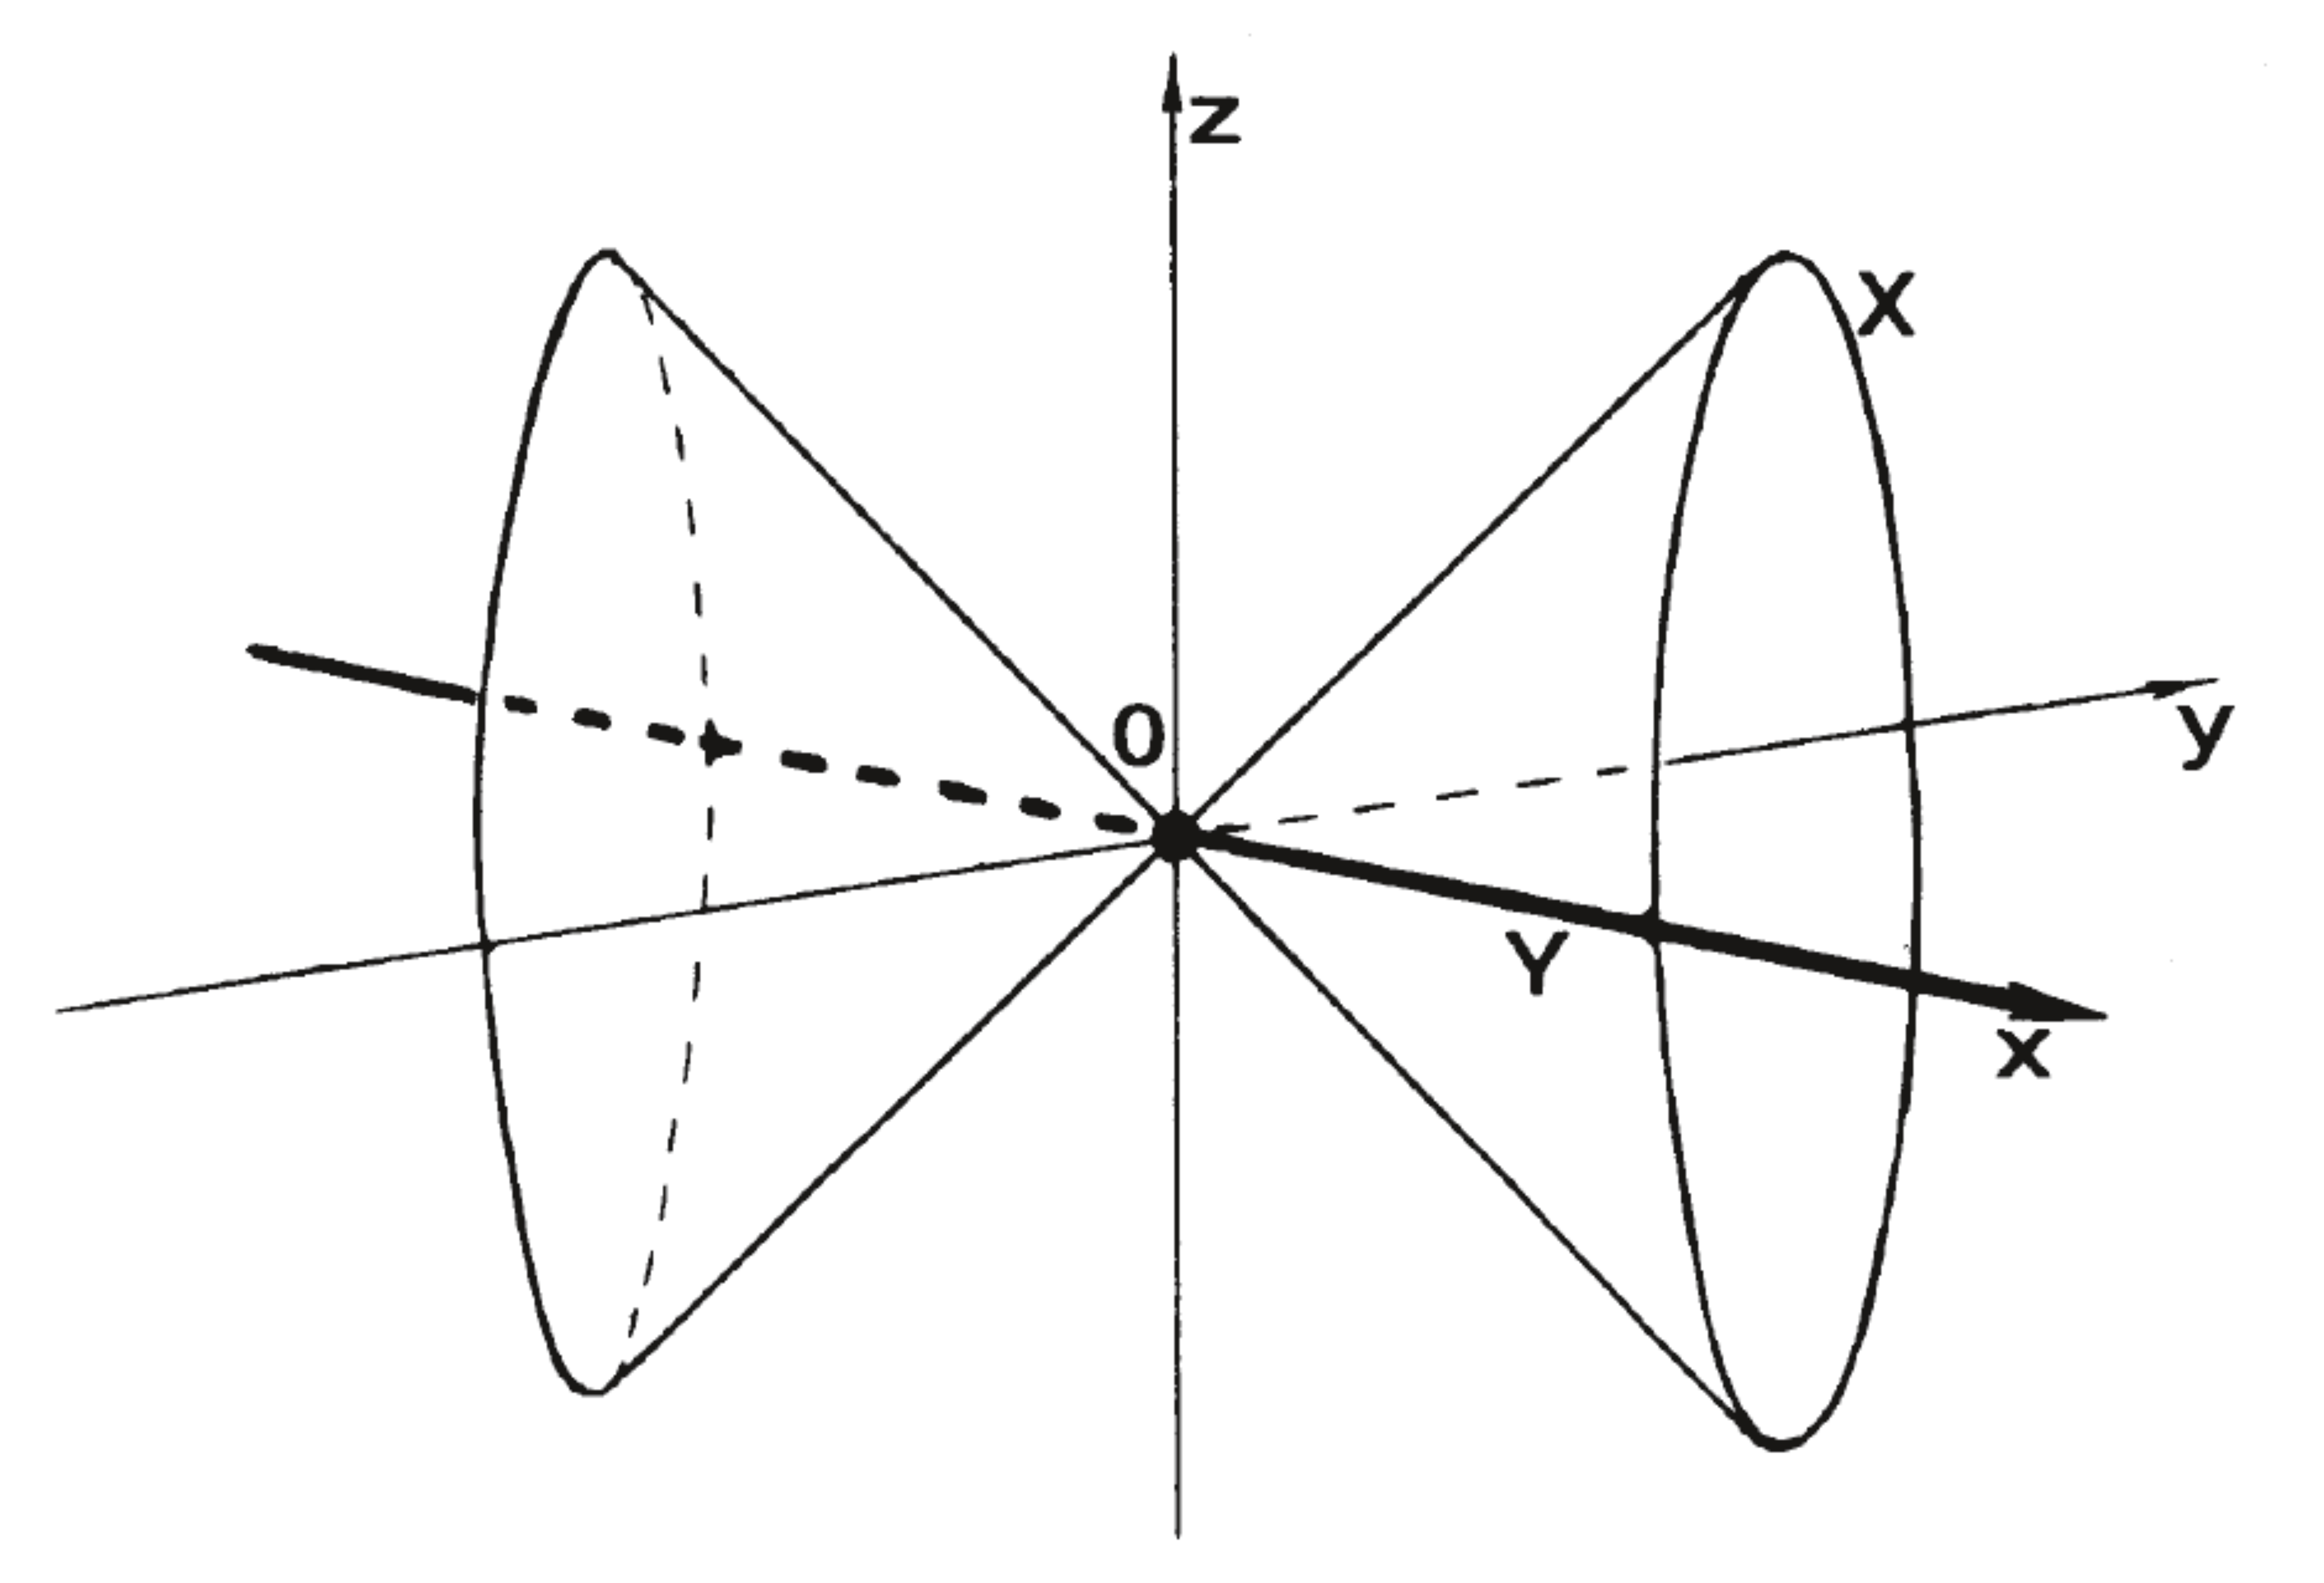
\includegraphics[width=7cm]{Figure8}\\
	Figure 8. 2차 원뿔 상에서의 모선
	\end{center}
	%
	여기에서 첫째 함수는 $1\mt 1\cdot Y$로 대응시킨다. 이제 $Y$는 함수 $y$에 의해 집합론적으로 잘라내질 수 있다.
	사실 $y=0\Ra z^2=0$이고 $z$가 $Y$의 일반점에서의 국소환의 극대 아이디얼을 생성하므로 $y$의 인자는 $2\cdot Y$이다.
	따라서 $X-Y=\Spec A_y$이다. 이제 $A_y=k[x,y,y^{-1},z]/(xy-z^2)$이다.
	이 환에서 $x=y^{-1}z^2$이므로 우리는 $x$를 제거할 수 있으며 $A_y\cong k[y,y^{-1},z]$임을 알 수 있다.
	이는 UFD이므로 (6.2)에 의해 $\Cl(X-Y)=0$이다.\\
	그러므로 우리는 $\Cl(X)$가 $Y$에 의해 생성되며 $2\cdot Y=0$임을 보였다. $T$ 자신이 주인자가 아님을 보이는 것이 남아있다.
	$A$가 정수적으로 닫혀 있으므로 (Ex. 6.4) 이는 $Y$의 소 아이디얼, 즉 $\mf p=(y,z)$가 주 아이디얼이 아님을 보이는 것과 동치이다.
	(cf. (6.2)의 증명) $\mf m=(x,y,z)$라 하고 $\mf m/\mf m^2$가 $x,y,z$의 상 $\bar x,\bar y,\bar z$에 의해 생성된
	$k$ 상에서의 3차원 벡터공간임을 기억해 두라.
	이제 $\mf p\bseq\mf m$이며 $\mf p$의 $\mf m/\mf m^2$에서의 상이 $\bar y$와 $\bar z$를 포함한다.
	따라서 $\mf p$는 주 아이디얼일 수 없다.
	\end{example}
	
	
	%Proposition 6.6
	\begin{proposition}
	$X$가 (*)를 만족시킨다 하자. 그 경우 $X\times\mb A^1(=X\times_{\Spec\Z}\Spec\Z[t])$도 (*)를 만족시키며
	$\Cl(X)\cong\Cl(X\times\mb A^1)$이다.\\\\
	%
	\pf 명백히 $X\times\mb A^1$은 정수적 Noether 분리 스킴이다.
	이것이 여차원 1에서 정칙임을 보이기 위해 $X\times\mb A^1$ 상에서 여차원 1인 점 $y$가 두 종류 존재함을 기억해 두어야 한다.
	종류 1은 $X$에서의 상이 여차원 1인 점 $y$인 점 $x$이다.
	이 경우 $\pi:X\times\mb A^1\ra X$가 사영이라 하면 $x$는 $\pi^{-1}(y)$의 일반점이다.
	그 국소환은 $\mc O_x\cong\mc O_y[t]_{\mf m_y}$이며 $\mc O_y$가 이산 부치환이므로 이는 명백히 이산 부치환이다.
	대응하는 소인자 $\overline{\{x\}}$는 단지 $\pi^{-1}(\overline{\{y\}})$이다.\\
	종류 2는 $X$에서의 상이 $X$의 일반점인 여차원 1의 점 $x\in X\times\mb A^1$이다.
	이 경우 $\mc O_x$는 $K[t]$의 어떠한 극대 아이디얼에서의 국소화이다. ($K$는 $X$의 함수체)
	$K[t]$가 주 아이디얼 정역이므로 이는 이산 부치환이다.
	그러므로 $X\times\mb A^1$도 (*)를 만족시킨다.\\
	함수 $\Cl X\ra\Cl(X\times\mb A^1)$을 $D=\sum n_iY_i\mt\pi^*D=\sum n_i\pi^{-1}(Y_i)$로 정의하자.
	만약 $f\in K^*$이면 $\pi^*((f))$는 $X\times\mb A^1$의 함수체 $K(t)$의 원소로 간주된 $f$의 인자이다.
	그러므로 이는 실제로 준동형사상 $\pi^*:\Cl X\ra\Cl(X\times\mb A^1)$이다.\\
	$\pi^*$가 단사임을 보이기 위해 $D\in\Div X$이며 어떠한 $f\in K(t)$에 대하여 $\pi^*D=(f)$라 하자.
	$\pi^*D$가 종류 1의 소인자만을 수반하므로 $f$는 $K$에 속해야 한다:
	그렇지 않다면 서로 소 $g,h\in K[t]$에 대하여 $f=g/h$로 표현 가능할 것이다.
	만약 $g,h$가 모두 $K$에 속하지 않는다면 $(f)$는 $X\times\mb A^1$ 상에서의 종류 2의 소인자를 수반할 것이다.
	이제 만약 $f\in K$이면 명백히 $D=(f)$이며 따라서 $\pi^*$가 단사이다.\\
	$\pi^*$가 전사임을 보이기 위해서는 $X\times\mb A^1$ 상에서의 임의의 종류 2의 소인자가
	종류 1의 소인자들의 선형 결합과 선형 동치임을 보이면 충분하다.
	그러므로 $Z\bseq X\times\mb A^1$이 종류 2의 소인자라 하자.
	$X$의 일반점에서 국소화하면 $\Spec K[t]$에서의 소인자를 얻으며 이는 소 아이디얼 $\mf p\bseq K[t]$에 대응한다.
	이는 주 아이디얼이며 따라서 $f$가 그 생성자라 하자.
	그 경우 $f\in K(t)$이며 $f$의 인자는 $Z$에 추가로 순수히 종류 1인 것이 더해질 수 있는 것으로 구성된다.
	이는 종류 2의 어떠한 소인자도 수반할 수 없다. 그러므로 $Z$는 순수히 종류 1인 인자와 선형 동치이다. 이는 증명을 완료한다.
	%
	\qed
	\end{proposition}
	
	
	%Example 6.6.1
	\begin{example}
	$Q$가 $\mb P^3_k$에서의 비특이 2차곡면 $xy=zw$라 하자. 우리는 $\Cl Q\cong\Z\oplus\Z$임을 보일 것이다.
	우리는 $Q$가 $\mb P_k^1\times_k\mb P_k^1$이라는 사실을 사용할 것이다. (I, Ex. 2.15)
	$p_1$과 $p_2$가 $Q$에서 두 인자로의 사영이라 하자.
	(6.6)의 증명에서와 마찬가지로 준동형사상 $p_1^*,p_2^*:\Cl\mb P^1\ra\Cl Q$를 얻는다.
	먼저 $p_1^*$와 $p_2^*$가 단사임을 보이자. $Y=pt\times\mb P^1$이라 하자. ($pt$는 닫힌 $k$-유리점)
	그 경우 $Q-Y=\mb A^1\times\mb P^1$이며 다음의 합성
	%
	$$\Cl\mb P^1\sr{p_2}\ra\Cl Q\ra\Cl(\mb A^1\times\mb P^1)$$
	%
	은 (6.6)의 동형사상이다. 따라서 $p_2^*$가 (마찬가지로 $p_1^*$도) 단사이다.\\
	이제 $Y$에 대한 (6.5)의 완전열을 고려하자:
	%
	$$\Z\ra\Cl Q\ra\Cl(\mb A^1\times\mb P^1)\ra 0$$
	%
	이 열에서 첫째 함수는 $1$을 $Y$로 대응시킨다.
	그러나 만약 우리가 $1$이 점의 동치류라 하는 것으로 $\Cl\mb P^1$을 $\Z$와 동일시하면 첫째 함수는 $p_1^*$이며 따라서 단사이다.
	우리가 방금 보인 것과 같이 $p_2^*$의 상이 동형적으로 $\Cl(\mb A^1\times\mb P^1)$로 대응되므로
	$\Cl Q\cong\Im p_1^*\oplus\Im p_2^*=\Z\oplus\Z$라 결론지을 수 있다.
	만약 $D$가 $Q$ 상에서의 임의의 인자이면 $(a,b)$가 $D$의 동치류에 대응하는 $\Z\oplus\Z$에 속한 정수들의 순서쌍이라 하자.
	그 경우 우리는 $D$가 $Q$ 상에서 \tb{종류(type)} $(a,b)$라 한다.
	\end{example}
	
	
	%Examle 6.6.2
	\begin{example}
	우리는 이차곡면 $Q\bseq\mb P^3$를 가지고 계속 진행하여 매장이 준동형사상 $\Cl\mb P^3\ra\Cl Q$를 유도함을 보이고
	$\Cl\mb P^3$을 생성하는 초평면 $H$의 상이 $\Cl Q=\Z\oplus\Z$에서의 원소 $(1,1)$임을 보일 것이다.
	$Y$가 $Q$를 포함하지 않는 $\mb P^3$의 임의의 기약 초곡면이라 하자.
	그 경우 우리는 $Y\cap Q$의 기약 성분들에 중복도를 부여하여 $Q$ 상에서의 \ti{인자} $Y\cdot Q$를 얻을 수 있다:
	$\mb P^3$의 각각의 표준 열린집합 $U_i$ 상에서 $Y$는 하나의 함수 $f$에 의해 정의된다;
	우리는 $Q$의 소인자의 각각의 부치에 대한 ($Q$로 제한된) 이 함수의 값을 취하여 인자 $Y\cdot Q$를 정의할 수 있다.
	선형성에 의해 우리는 이 함수를 확장하여 어떠한 $Y_i$도 $Q$를 포함하지 않도록 하는 $\mb P^3$ 상에서의 각각의 인자
	$D=\sum n_iY_i$에 대하여 $Q$ 상에서의 인자 $D\cdot Q$를 정의할 수 있다.
	명백히 선형 동치 인자들은 선형 동치 인자들로 제한된다.
	(6.4)에 의해 $\mb P^3$ 상에서의 임의의 인자가 소인자들이 $Q$를 포함하지 않도록 하는 인자와 선형 동치이므로
	잘 정의된 준동형사상 $\Cl\mb P^3\ra\Cl Q$를 얻는다.
	이제 만약 $H$가 초평면 $w=0$이면 $H\cap Q$는 두 직선 $x=w=0$과 $y=w=0$으로 구성된 인자이다.
	이들은 각각 직선들의 족에 속하므로 (I, Ex. 2.15) $H\cap Q$는 $\Cl Q=\Z\oplus\Z$에서 종류 $(1,1)$이다.
	직선들의 두 족이 $pt\times\mb P^1$과 $\mb P^1\times pt$에 대응함을 기억해 두라.
	따라서 이들은 $(1,0)$과 $(0,1)$이다.
	\end{example}
	
	
	%Example 6.6.3
	\begin{example}
	이 예시를 한 단계 더 진행하여, $C$가 $Q$에 속한 비틀린 3차곡선 $x=t^3,y=u^3,z=t^2u,w=tu^2$라 하자.
	만약 $Y$가 2차 원뿔 $yz=w^2$이면 $L$이 직선 $y=w=0$이라 할 때 $Y\cap Q=C\cup L$이다.
	$\mb P^3$ 상에서 $Y\sim 2H$이므로 $Y\cap Q$는 종류 $(2,2)$의 인자이다.
	직선 $L$이 종류 $(1,0)$이므로 $C$는 종류 $(1,2)$이다.
	$Q$를 포함하지 않는 어떠한 곡면 $Y\bseq\mb P^3$도 $Y\cap Q=C$를 (집합론적으로조차도) 만족시킬 수 없음이 따라온다:
	이 경우 인자 $Y\cap C$는 어떠한 정수 $r>0$에 대하여 $rC$가 되어야 한다.
	이는 $\Cl Q$에서의 종류 $(r,2r)$의 인자이다.
	그러나 만약 $Y$가 $d$차곡면이면 $Y\cap Q$는 종류 $(d,d)$이며 이는 절대 $(r,2r)$이 될 수 없다. 따라서 $Y$가 존재하지 않는다.
	\end{example}
	
	
	%Example 6.6.4
	\begin{example}
	우리는 나중에 (V, 4.8) 만약 $X$가 $\mb P^3$에서의 비특이 3차곡면이면 $\Cl X\cong\Z^7$임을 보게 될 것이다.
	\end{example}
	
	
	
	%Subsection
	\subsection*{Divisors on Curves (곡선 상에서의 인자)}
	
	우리는 곡선 상에서의 인자들의 경우에 특별한 주의를 기울이는 것으로 인자류군의 개념을 설명할 것이다.
	우리는 곡선 상에서의 인자의 차수를 정의할 것이며 완비 비특이 곡선 상에서 차수가 선형 동치 하에서 안정함을 보일 것이다.
	곡선 상에서의 인자에 대한 심화된 내용은 Chapter IV에서 찾을 수 있을 것이다.
	
	시작하기에 앞서 곡선 및 곡선의 사상에 대한 선행 지식이 필요하다.
	Section 4의 끝부분에서의 관습과 용어를 상기하라:
	
	
	%Definition
	\begin{definition}
	$k$가 대수적으로 닫힌 체라 하자. $k$ 상에서의 \tb{곡선(curve)}은 $k$ 상에서의 1차원 유한형 정수적 분리 스킴 $X$이다.
	만약 $X$가 $k$ 상에서 진이면 $X$가 \tb{완비(complete)}라 한다.
	만약 $X$의 모든 국소환이 정칙 국소환이면 $X$가 \tb{비특이(nonsingular)}라 한다.
	\end{definition}
	
	
	%Proposition 6.7
	\begin{proposition}
	$X$가 $k$ 상에서의 비특이 곡선이며 함수체 $K$를 가진다 하자. 그 경우 다음의 조건들은 동치이다:\\
	%
	\begin{enumerate}[label=(\roman*)]
	\item $X$가 사영이다.
	\item $X$가 완비이다.
	\item (I, \S 6)의 추상적 비특이 곡선 $C_K$와 (2.6)의 대수다양체에서 스킴으로의 함자 $t$에 대하여 $X\cong t(C_K)$이다.\\
	\end{enumerate}
	%
	\pf (i) $\Ra$ (ii) (4.9)에서 따라온다.\\
	(ii) $\Ra$ (iii) 만약 $X$가 완비이면 $K/k$의 모든 이산 부치환은 $X$ 상에서의 유일한 중심을 가진다. (Ex. 4.5)
	닫힌점에서의 $X$의 국소환들은 모두 이산 부치환이므로 이는 $X$의 닫힌점들이 $K/k$의 이산 부치환들,
	즉 $C_K$의 점들과 1-1 대응함을 함의한다. 그러므로 $X\cong t(C_K)$임이 자명하다.\\
	(iii) $\Ra$ (i) (I, 6.9)에서 따라온다.
	%
	\qed
	\end{proposition}
	
	
	%Proposition 6.8
	\begin{proposition}
	$X$가 $k$ 상에서의 완비 비특이 곡선이며 $Y$가 $k$ 상에서의 임의의 곡선이고 $f:X\ra Y$가 사상이라 하자.
	그 경우 (1) $f(X)=$한 점이거나 (2) $f(X)=Y$이다.
	(2)의 경우 $K(X)$는 $K(Y)$의 유한 확대체이고 $f$가 유한 사상이며 $Y$도 완비이다.\\\\
	%
	\pf $X$가 완비이므로 $f(X)$는 $Y$에서 닫혀 있어야 하며 $\Spec k$ 상에서 진이다. (Ex. 4.4)
	또한 $f(X)$가 기약이다. 그러므로 (1) $f(X)=pt$ 또는 (2) $f(X)=Y$이며 (2)의 경우 $Y$도 완비이다.\\
	(2)의 경우 $f$가 우세이며 따라서 이는 함수체의 포함 준동형사상 $K(Y)\bseq K(X)$를 유도한다.
	두 체가 모두 $k$의 초월 차수 1의 유한생성 확대이므로 $K(X)$는 $K(Y)$의 유한 대수적 확대여야 한다.
	$f$가 유한 사상임을 보이기 위해 $V=\Spec B$가 $Y$의 임의의 아핀 열린 부분집합이라 하자.
	$A$가 $B$의 $K(X)$에서의 정수적 폐포라 하자.
	그 경우 $A$는 유한 $B$-모듈이며 (I, 3.9A) $\Spec A$는 $X$의 열린 부분집합 $U$와 동형이다. (I, 6.7)
	명백히 $U=f^{-1}V$이며 따라서 이는 $f$가 유한 사상임을 보여준다.
	%
	\qed
	\end{proposition}
	
	
	%Definition
	\begin{definition}
	만약 $f:X\ra Y$가 곡선 간의 유한 사상이면 $f$의 \tb{차수(degree)}를 체 확대 $[K(X):K(Y)]$의 차수로 정의한다.
	\end{definition}
	
	이제 우리는 곡선 상에서의 인자를 다룰 것이다.
	만약 $X$가 비특이 곡선이면 $X$는 앞에서 사용된 조건 (*)를 만족시키며 따라서 우리는 $X$ 상에서의 인자에 대해 말할 수 있다.
	소인자는 단지 닫힌점이며 따라서 임의의 인자는 닫힌점 $P_i$들과 $n_i\in\Z$에 대하여 $D=\sum n_iP_i$로 표현 가능하다.
	$D$의 \tb{차수(degree)}를 $\sum n_i$로 정의한다.
	
	
	%Definition
	\begin{definition}
	만약 $f:X\ra Y$가 비특이 곡선 간의 유한 사상이면 준동형사상 $f^*:\Div Y\ra\Div X$를 다음과 같이 정의한다.
	임의의 점 $Q\in Y$에 대하여 $t\in\mc O_Q$가 $Q$에서의 \tb{국소매개변수(local parameter)}라 하자.
	i.e. 이산 부치환 $\mc O_Q$에 대응하는 부치를 $v_Q$라 하면 $t$는 $v_Q(t)=1$을 만족시키는 $K(Y)$의 원소이다.
	우리는 $f^*Q=\sum_{f(P)=Q}v_P(t)\cdot P$로 정의한다.
	$f$가 유한 사상이므로 이는 유한합이며 따라서 우리는 $X$ 상에서의 인자를 얻는다.
	$f^*Q$가 국소매개변수 $t$의 선택에 독립적임을 기억해 두라:
	만약 $t'$이 $Q$에서의 다른 국소매개변수이면 $\mc O_Q$에서의 가역원 $u$에 대하여 $t'=ut$이다.
	$f(P)=Q$를 만족시키는 임의의 점 $P\in X$에 대하여 $u$는 $\mc O_P$에서의 가역원일 것이며 따라서 $v_P(t)=v_P(t')$이다.
	이 정의를 선형성에 의해 $Y$ 상에서의 모든 인자들로 확대한다.
	$f^*$가 선형 동치를 보존함을 간단히 보일 수 있으며 따라서 이는 준동형사상 $f^*:\Cl Y\ra\Cl X$를 유도한다.
	\end{definition}
	
	
	%Proposition 6.9
	\begin{proposition}
	$f:X\ra Y$가 비특이 곡선 간의 유한 사상이라 하자.
	그 경우 $Y$ 상에서의 임의의 인자 $D$에 대하여 $\deg f^*D=\deg f\cdot\deg D$이다.\\\\
	%
	\pf 임의의 닫힌점 $Q\in Y$에 대하여 $\deg f^*Q=\deg f$임을 보이면 충분하다.
	$V=\Spec B$가 $Q$를 포함하는 $Y$의 아핀 열린 부분집합이라 하자.
	그 경우 (6.8)의 증명에서와 마찬가지로 $U=\Spec A$는 $X$의 열린 부분집합 $f^{-1}V$이다.
	$\mf m_Q$가 $Q$의 $B$에서의 극대 아이디얼이라 하자. $B$와 $A$를 모두 곱셈적 체계 $S=B-\mf m_Q$에 대하여 국소화하면
	환의 확대 $\mc O_Q\hra A'$을 얻는다. (여기에서 $A'$은 유한생성 $\mc O_Q$-모듈이다.)
	이제 $A'$은 비틀림 없는 모듈이며 계수 $r=[K(X):K(Y)]$를 가진다.
	따라서 $A'$은 계수 $r=\deg f$의 자유 $\mc O_Q$-모듈이다.
	만약 $t$가 $Q$에서의 국소매개변수이면 $A'/tA'$가 $r$차원 $k$-벡터 공간임이 따라온다.\\
	또한 $f(P_i)=Q$를 만족시키는 $X$의 점 $P_i$들은 $A'_{\mf m_i}=\mc O_{P_i}$를 만족시키는
	$A'$의 극대 아이디얼 $\mf m_i$들과 1-1 대응한다.
	명백히 $tA'=\bigcap_i(tA'_{\mf m_i}\cap A')$이며 따라서 중국인의 나머지 정리에 의해 다음이 성립한다.
	%
	$$\dim_k(A'/tA')=\sum_i\dim_kA'/(tA'_{\mf m_i}\cap A')$$
	%
	그러나,
	%
	$$A'/(tA'_{\mf m_i}\cap A')\cong A'_{\mf m_i}/tA'_{\mf m_i}=\mc O_{P_i}/t\mc O_{P_i}$$
	%
	따라서 위 합의 차원들은 $v_{P_i}(t)$와 같다. 그러나 $f^*Q=\sum v_{P_i}(t)\cdot P_i$이므로
	우리는 요구된 것과 같이 $\deg f^*Q=\deg f$임을 보였다.
	%
	\qed
	\end{proposition}
	
	
	%Corollary 6.10
	\begin{corollary}
	완비 비특이 곡선 $X$ 상에서의 주인자는 차수 0이다. 결과적으로 차수 함수는 전사 준동형사상 $\mrm{deg}:\Cl X\ra\Z$를 유도한다.\\\\
	%
	\pf $f\in K(X)^*$라 하자. 만약 $f\in k$이면 $(f)=0$이며 따라서 증명할 것이 없다.
	만약 $f\notin k$이면 체의 포함 관계 $k(f)\bseq K(X)$는 유한 사상 $\ph:X\ra\mb P^1$을 유도한다.
	(I, 6.12)에 의해 이는 사상이며 (6.8)에 의해 이는 유한이다. 이제 $(f)=\ph^*(\{0\}-\{\infty\})$이다.
	$\{0\}-\{\infty\}$가 $\mb P^1$ 상에서의 차수 0의 인자이므로  $(f)$가 $X$에서 차수 0이라 결론지을 수 있다.\\
	그러므로 $X$ 상에서의 인자의 차수는 그 선형 동치류에만 의존하며 명시된 것과 같이 준동형사상 $\Cl X\ra\Z$를 얻는다.
	한 점의 차수가 1이므로 이는 전사이다.
	%
	\qed
	\end{corollary}
	
	
	%Example 6.10.1
	\begin{example}
	완비 비특이 곡선 $X$가 유리일 필요충분조건은 서로 다른 두 점 $P,Q\in X$가 존재하여 $P\sim Q$인 것이다:
	(\tb{유리(rational)}임이 $\mb P^1$과 쌍유리동치임을 의미함을 상기하라.)
	만약 $X$가 유리이면 이는 사실 (6.7)에 의해 $\mb P^1$과 동형이다.
	또한 $\mb P^1$ 상에서 임의의 두 점이 선형 동치임을 (6.4)에서 이미 보였다.
	역으로 $X$가 $P\sim Q$인 두 점 $P\ne Q$를 가진다 하자. 그 경우 $f\in K(X)$가 존재하여 $(f)=P-Q$이다.
	(6.10)의 증명에서와 같이 $f$에 의해 결정된 사상 $\ph:X\ra\mb P^1$을 고려하자.
	$\ph^*(\{0\})=P$이며 따라서 $\ph$는 차수 1의 사상이어야 한다. 다르게 표현하면 $\ph$가 쌍유리이며 따라서 $X$가 유리이다.
	\end{example}
	
	
	%Example 6.10.2
	\begin{example}
	$X$가 $\Char k\ne 2$인 $\mb P_k^2$에서의 비특이 3차곡선 $y^2z=x^3-xz^2$라 하자.
	우리는 이미 $X$가 유리가 아님을 보였다. (I, Ex. 6.2)
	$\Cl^\circ X$가 차수 준동형사상 $\Cl X\ra\Z$의 핵이라 하자. 그 경우 위 예시에 의해 $\Cl^\circ X\ne 0$임을 알 수 있다.
	$X$의 닫힌점들과 군 $\Cl^\circ X$의 원소들 간에 자연스러운 1-1 대응이 존재함을 보일 것이다.
	이는 군 $\Cl^\circ X$의 구조를 명확히 밝혀 준다.
	또한 이는 $X$의 닫힌점들의 집합에 군 구조를 부여하며 따라서 $X$를 군 대수다양체로 만든다. (Fig. 9)
	%
	\begin{center}
	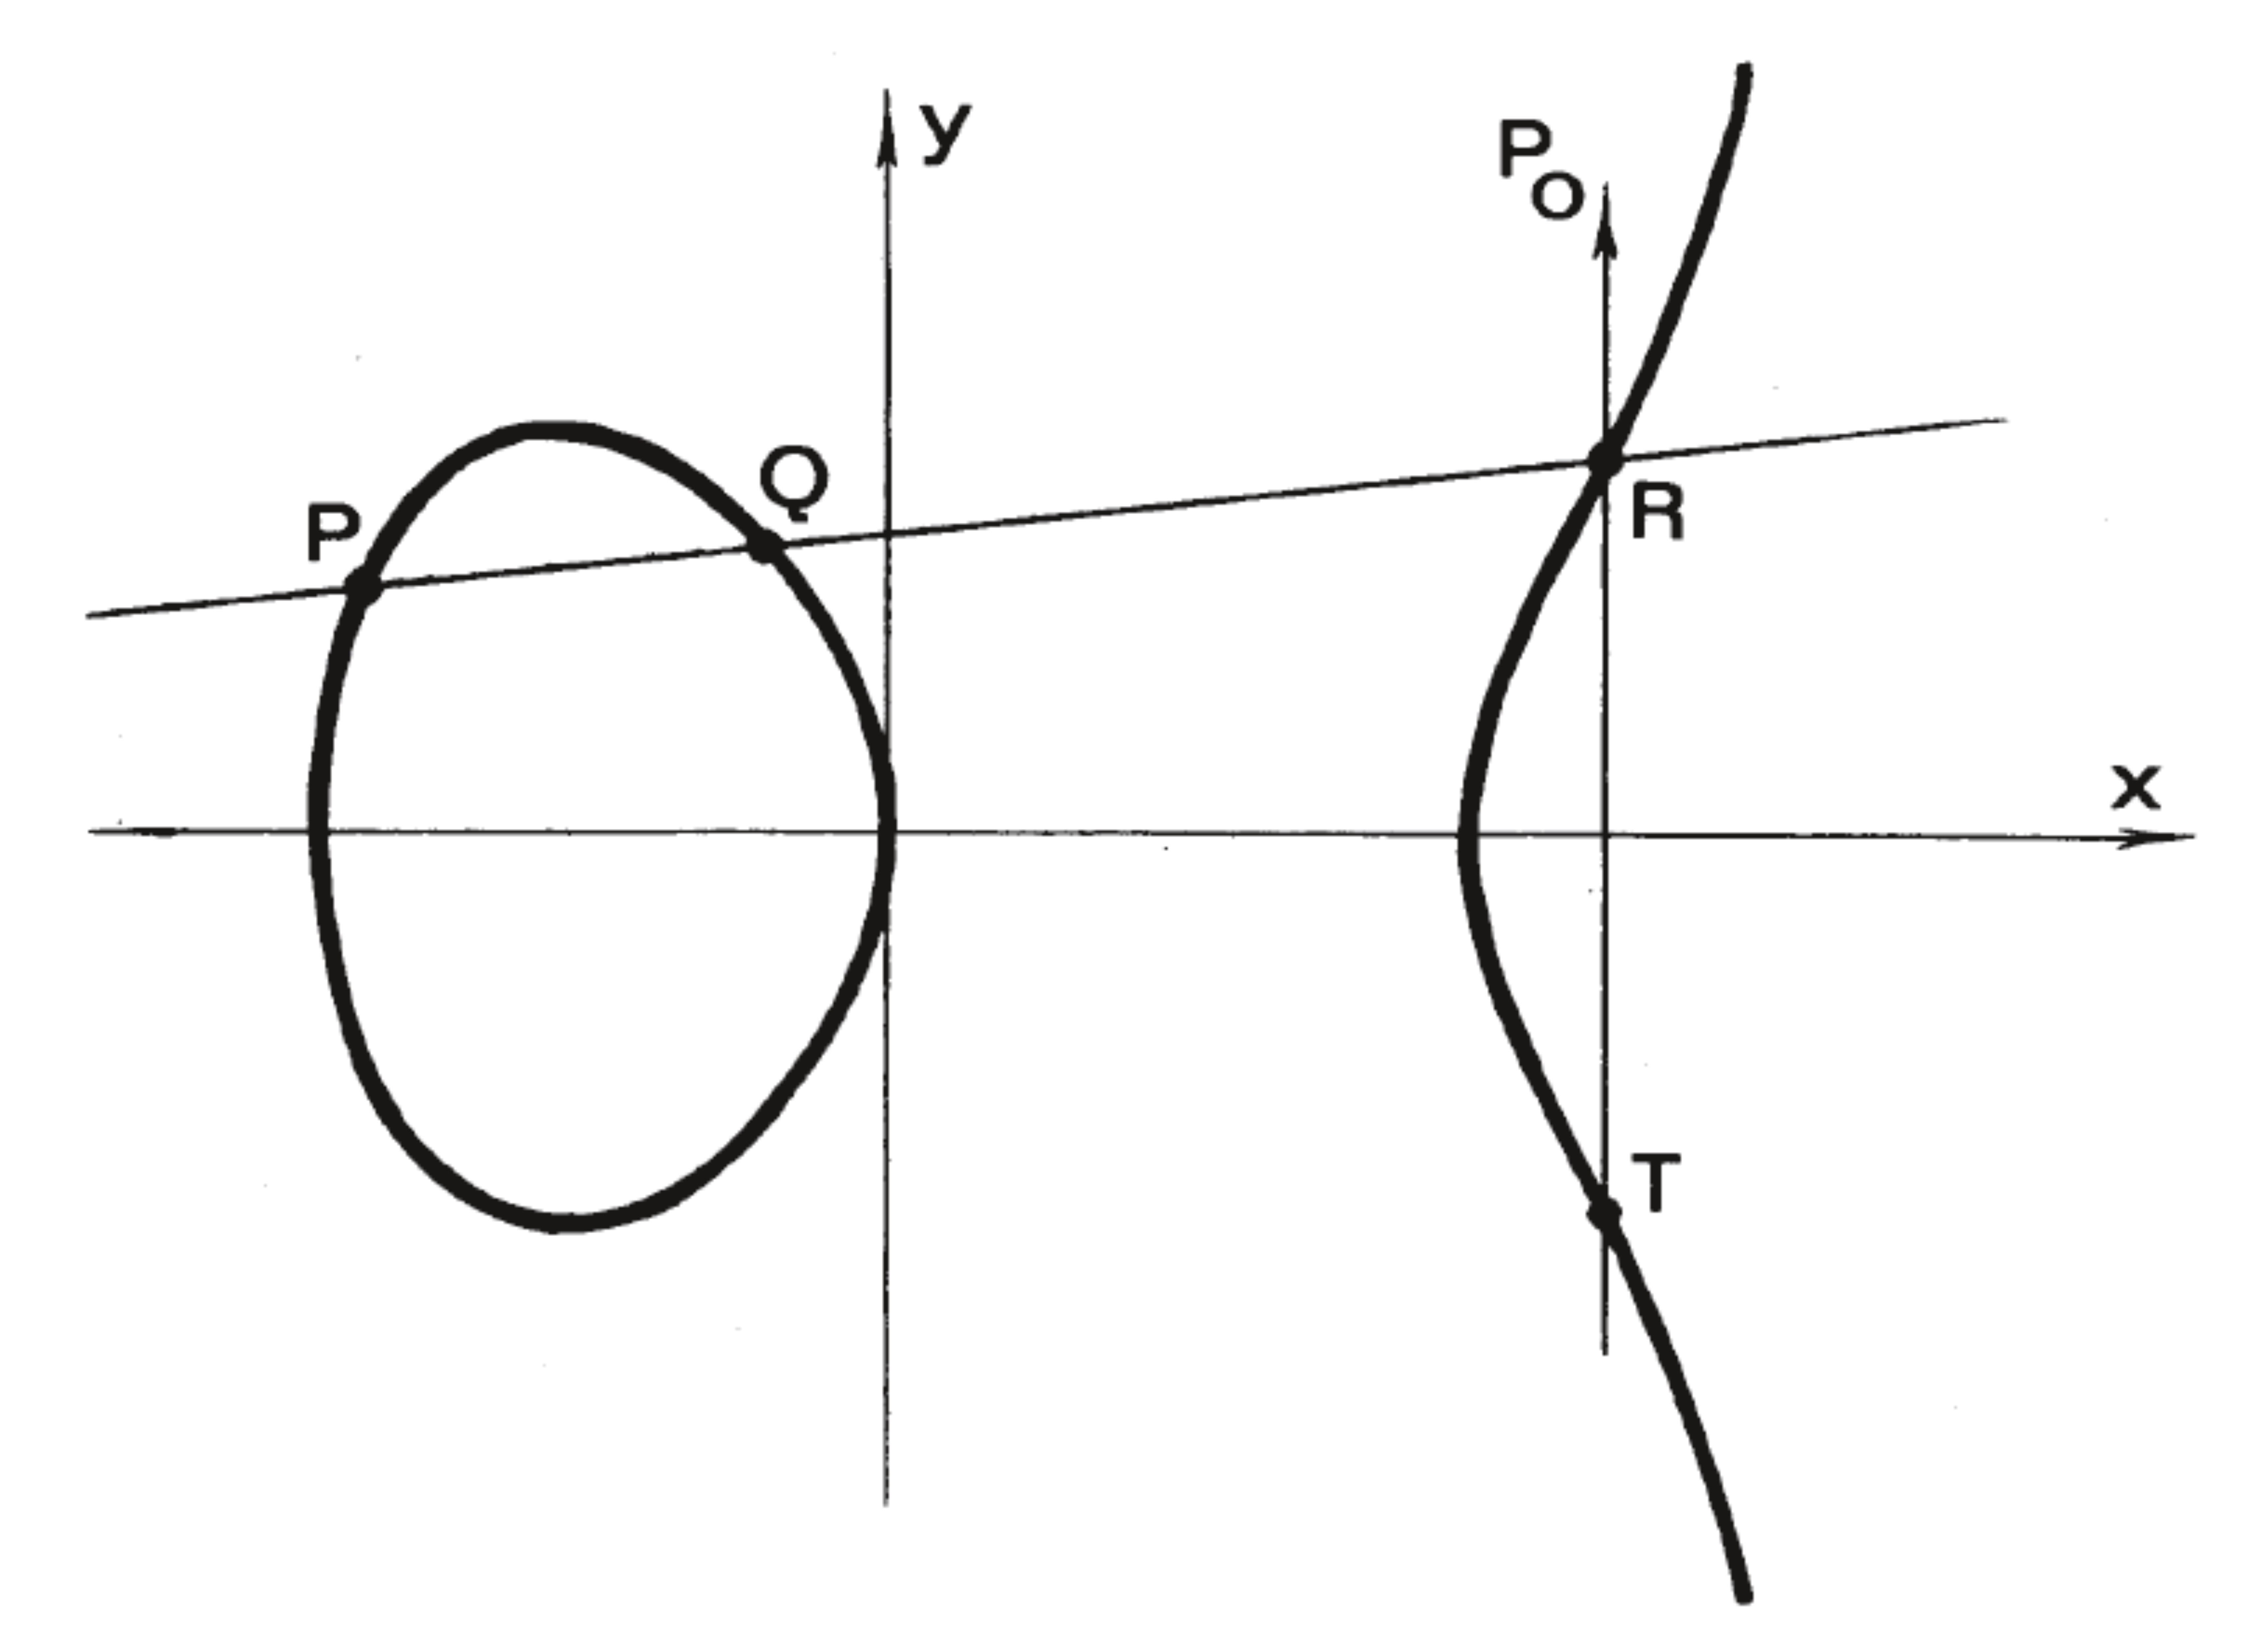
\includegraphics[width=7cm]{Figure9}\\
	Figure 9. 3차곡선 상에서의 군 연산
	\end{center}
	%
	$P_0$가 $X$ 상에서의 점 $(0,1,0)$이라 하자. 이는 변곡점이며 따라서 이 점에서의 접선 $z=0$는 곡선과 인자 $3P_0$에서 만난다.
	만약 $L$이 $\mb P^2$에서의 임의의 다른 직선이며 $X$와 세 점 $P,Q,R$에서 만나면 (이들은 서로 일치할 수도 있다)
	$L$이 $\mb P^2$에서 직선 $z=0$과 선형 동치이므로 위 (6.6.2)에서와 같이 $X$ 상에서 $P+Q+R\sim 3P_0$가 성립한다.\\
	이제 임의의 닫힌점 $P\in X$에 대하여 우리는 인자 $P-P_0\in\Cl X$를 대응시킬 것이다.
	이 함수는 단사이다: 만약 $P-P_0\sim Q-P_0$이면 $P\sim Q$이며 $X$가 유리가 아니므로 위 예시에 의해 이것이 불가능하다.\\
	이 함수가 $X$의 닫힌점들에서 $\Cl^\circ X$로의 전사 함수임을 보이기 위해서는 여러 단계가 필요하다.
	$D\in\Cl^\circ X$라 하자. 그 경우 $D=\sum n_iP_i$이며 $\sum n_i=0$이다.
	따라서 우리는 $D=\sum n_i(P_i-P_0)$로도 표현할 수 있다.
	이제 임의의 점 $R$에 대하여 직선 $P_0R$이 $X$와 다른 점 $T$에서 만난다고 하자.
	(교집합을 항상 중복도를 가지고 센다 - 예를 들어 만약 $R=P_0$이면 직선 $P_0R$을 $P_0$의 접선으로 취하며 셋째 교점 $T$도 $P_0$이다.)
	그 경우 $P_0+R+T\sim 3P_0$이며 따라서 $R-P_0\sim -(T-P_0)$이다.
	만약 $i$가 $D$에서 $n_i<0$을 만족시키는 첨자이면 $P_i=R$로 선택한다.
	그 후 $P_i$를 $T$로 대체하면 $i$번째 계수 $-n_i>0$인 선형 동치 인자를 얻는다.
	이 과정을 반복하면 우리는 $D=\sum n_i(P_i-P_0)$에서 모든 $n_i>0$이라 가정할 수 있다.
	이제 우리는 $\sum n_i$에 대한 귀납법으로 어떠한 점 $P$에 대하여 $D\sim P-P_0$임을 보일 것이다.
	만약 $\sum n_i=1$이면 증명할 것이 없다.
	그러므로 $\sum n_i\ge 2$이며 $P,Q$가 $D$에서 등장하는 점 $P_i$들 중 두 개(서로 같을 수 있다)라 하자.
	직선 $PQ$가 $X$와 $R$에서 만난다 하고 직선 $P_0R$이 $X$와 $T$에서 만난다 하자. 그 경우 다음이 성립한다.
	%
	$$P+Q+R\sim 3P_0\qcq P_0+R+T\sim 3P_0$$
	%
	따라서,
	%
	$$(P-P_0)+(Q-P_0)\sim(T-P_0)$$
	%
	$P$와 $Q$를 $T$로 대체하면 $D$가 $\sum n_i$가 하나 작은 다른 인자와 선형 동치임을 얻으며
	따라서 귀납법에 의해 어떠한 $P$에 대하여 $D\sim P-P_0$이다.\\
	그러므로 우리는 군 $\Cl^\circ X$가 $X$의 닫힌점들의 집합과 1-1 대응함을 보였다.
	이러한 덧셈 연산이 사상 $X\times X\ra X$를 결정하며 역원 연산이 사상 $X\ra X$를 결정함을 직접적으로 보일 수 있다.
	(예를 들어 Olson [1]을 참조하라.) 그러므로 $X$는 (I, Ex. 3.21)에서의 의미로 군 대수다양체이다.
	일반화를 위해서는 (IV, 1.3.7)을 참조하라.
	\end{example}
	
	
	%Remark 6.10.3
	\begin{remark}
	이러한 3차곡선 예시는 대수다양체의 인자류군이 이산적인 성분(이 경우 $\Z$)과
	스스로 대수다양체 구조를 가지는 연속적인 성분(이 경우 $\Cl^\circ X$)을 가진다는 일반적인 사실을 보여준다.\\
	더 구체적으로, 만약 $X$가 임의의 완비 비특이 곡선이면 군 $\Cl^\circ X$는
	$X$의 \tb{Jacobi 대수다양체(Jacobian variety)}라 불리는 Abel 대수다양체의 닫힌점들의 군과 동형이다.\\
	만약 $X$가 차원 2 이상의 비특이 사영 대수다양체이면 우리는 $\Cl X$의 부분군 $\Cl^\circ X$,
	즉 \tb{대수적으로 0과 동치(algebraically equivalent to zero)}인 인자류들의 부분군을
	$\Cl X/\Cl^\circ X$가 $X$의 \tb{N\'eron-Severi 군(N\'eron-Severi group)}이라 불리는 가환군이며
	$\Cl^\circ X$가 $X$의 \tb{Picard 대수다양체(Picard variety)}라 불리는
	Abel 대수다양체의 닫힌점들의 군과 동형이도록 정의할 수 있다.\\
	불운히도 이 책에는 Abel 대수다양체의 이론을 개발하고 주어진 대수다양체의 Jacobian 및 Picard 대수다양체를 연구할 충분한 공간이 없다.
	이 아름다운 주제에 대한 추가적인 정보와 참고문헌을 위해서는 Lang [1], Mumford [2], Mumford [5], Hartshorne [6]을 참조하라.
	(IV, \S4), (V, Ex. 1.7), Appendix B도 참조하라.
	\end{remark}
	
	
	%Subsection
	\subsection*{Cartier Divisors (Cartier 인자)}
	
	이제 우리는 인자의 개념을 임의의 스킴으로 확장하고자 한다.
	여차원 1의 기약 부분대수다양체들을 사용하는 것은 잘 작동하지 않는다는 것이 드러난다.
	그러므로 대신 우리는 인자는 국소적으로 유리함수의 인자처럼 보이는 것이어야 한다는 발상을 출발점으로 선택할 것이다.
	이는 (우리가 보일 것과 같이) 정확히 Weil 인자의 일반화는 아니지만 임의의 스킴 상에서 사용하기 좋은 개념을 제공한다.
	
	
	%Definition
	\begin{definition}
	$X$가 스킴이라 하자. 각각의 아핀 열린 부분집합 $U=\Spec A$에 대하여 $S$가 영인자가 아닌 $A$의 원소들의 집합이며
	$K(U)$가 곱셈적 체계 $S$에 의한 $A$의 국소화라 하자. 우리는 $K(U)$를 $A$의 \tb{전분수환(total quotient ring)}이라 한다.
	각각의 열린집합 $U$에 대하여 $S(U)$가 각각의 $x\in U$에 대하여 국소환 $\mc O_x$에서 영인자가 아닌
	$\Ga(U,\mc O_X)$의 원소들의 집합을 나타낸다 하자.
	그 경우 환 $S(U)^{-1}\Ga(U,\mc O_X)$는 준층을 형성하며 여기에 연관된 환의 층 $\ms K$를
	$\mc O$의 \tb{전분수환의 층(sheaf of total quotient rings)}이라 한다.
	임의의 스킴 상에서 층 $\ms K$는 정수적 스킴의 함수체의 개념을 대체한다.
	환의 층 $\ms K$의 가역원들의 (곱셈군의) 층을 $\ms K^*$로 나타낸다.
	마찬가지로 $\mc O^*$는 $\mc O$에서의 가역원들의 층이다.
	\end{definition}
	
	
	%Definition
	\begin{definition}
	스킴 $X$ 상에서의 \tb{Cartier 인자(Cartier divisor)}는 층 $\ms K^*/\ms O^*$의 대역적 단면이다.
	몫층의 성질들을 생각해 보면 $X$ 상에서의 Cartier 인자들은 $X$의 열린 덮개 $\{U_i\}$와
	각각의 $i$에 대하여 다음을 만족시키는 원소 $f_i\in\Ga(U_i,\ms K^*)$들을 제시하는 것으로 기술된다:
	각각의 $i,j$에 대하여 $f_i/f_j\in\Ga(U_i\cap U_j,\mc O^*)$.
	Cartier 인자가 \tb{주(principal)}인자라는 것의 정의는 자연스러운 함수 $\Ga(X,\ms K^*)\ra\Ga(X,\ms K^*/\ms O^*)$의 상인 것이다.
	두 Cartier 인자가 \tb{선형 동치(linearly equivalent)}라는 것의 정의는 이들의 차가 주인자인 것이다.
	($\ms K^*/\ms O^*$ 상에서의 군 연산이 곱셈임에도 불구하고 Weil 인자와의 유사성을 보존하기 위해
	우리는 Cartier 인자에 대하여 말할 경우 가환군의 언어를 사용할 것이다.)
	\end{definition}
	
	
	%Proposition 6.11
	\begin{proposition}
	$X$가 정수적 분리 Noether 스킴이며 그 국소환들이 모두 유일 인수분해 정역이라 하자.
	(이 경우 우리는 $X$가 \tb{국소 인수분해 가능(locally factorial)}이라 한다.)
	그 경우 $X$ 상에서의 Weil 인자들의 군 $\Div X$는 Cartier 인자들의 군 $\Ga(X,\ms K^*/\mc O^*)$과 동형이다.
	또한 이러한 동형사상 하에서 Weil 주인자들은 Cartier 주인자에 대응한다.\\\\
	%
	\pf 먼저 UFD가 정수적으로 닫혀 있으므로 $X$가 정규이며 따라서 (*)를 만족시킴을 기억해 두라.
	그러므로 Weil 인자가 잘 정의된다. $X$가 정수적이므로 층 $\ms K$는 $X$의 함수체 $K$에 대응하는 상수층이다.
	이제 Cartier 인자가 $X$의 열린 덮개 $\{U_i\}$와 $f_i\in\Ga(U_i,\ms K^*)=K^*$에 대하여 $\{(U_i,f_i)\}$로 주어진다 하자.
	우리는 연관된 Weil 인자를 다음과 같이 정의할 것이다. 각각의 소인자 $Y$에 대하여 $Y$의 계수를 $v_Y(f_i)$로 취한다.
	여기에서 $i$는 $Y\cap U_i\ne\es$를 만족시키는 임의의 첨자이다.
	만약 $j$가 이러한 다른 인자이면 $f_i/f_j$가 $U_i\cap U_j$ 상에서 가역이며 따라서 $v_Y(f_i/f_j)=0$이고 $v_Y(f_i)=v_Y(f_j)$이다.
	그러므로 우리는 잘 정의된 $X$ 상에서의 Weil 인자 $D=\sum v_Y(f_i)Y$를 얻는다. ($X$가 Noether이므로 합이 유한합이다.)\\
	역으로 만약 $D$가 $X$ 상에서의 Weil 인자이며 $x\in X$가 임의의 점이라 하자.
	그 경우 $D$는 국소 스킴 $\Spec\mc O_x$에서의 Weil 인자 $D_x$를 유도한다.
	$\mc O_x$가 UFD이므로 (6.2)에 의해 $D_x$는 주인자이며 따라서 어떠한 $f_x\in K$에 대하여 $D_x=(f_x)$이다.
	이제 $X$ 상에서의 주인자 $(f_x)$는 $\Spec\mc O_x$로의 제한이 $D$와 동일하므로
	이들은 $x$를 지나지 않는 소인자들에서만 다를 수 있다.
	$D$ 또는 $(f_x)$에서 0이 아닌 계수를 가지는 것은 유한 개뿐이므로 $x$의 열린 근방 $U_x$가 존재하여
	$D$와 $(f_x)$의 $U_x$로의 제한이 같도록 한다.
	$X$를 이러한 열린집합 $U_x$들로 덮으면 함수 $f_x$들은 $X$ 상에서의 Cartier 인자를 준다.
	만약 $f,f'$이 열린집합 $U$ 상에서 동일한 Weil 인자를 준다면 $X$가 정규이므로 $f/f'\in\Ga(U,\mc O^*)$이다.
	(cf. (6.2)의 증명) 그러므로 잘 정의된 Cartier 인자를 얻는다.\\
	이러한 두 구축은 서로의 역이며 따라서 우리는 Weil 인자와 Cartier 인자의 군이 동형임을 알 수 있다.
	주인자들이 서로 대응됨은 명백하다.
	%
	\qed
	\end{proposition}
	
	
	%Remark 6.11.1A
	\begin{remarka}
	정칙 국소환이 UFD이므로 (Matsumura [2, Th. 48, p. 142]) 이 명제는 특히 임의의 \ti{정칙} 정수적 분리 Noether 스킴에 적용 가능하다.
	스킴이 \tb{정칙(regular)}임은 모든 국소환이 정칙 국소환인 것이다.
	\end{remarka}
	
	
	%Remark 6.11.2
	\begin{remark}
	만약 $X$가 국소 인수분해 가능할 필요는 없는 정규 스킴이면 Weil 국소주인자들로 구성된 $\Div X$의 부분군을 정의할 수 있다:
	$D$가 \tb{국소주(locally principal)}인자라는 것의 정의는 $D\rest_U$가 주인자이도록 하는 $U$들로 $X$를 덮을 수 있는 것이다.
	그 경우 위 증명은 Cartier 인자들은 Weil 국소주인자들과 같음을 보여준다.
	\end{remark}
	
	
	%Example 6.11.3
	\begin{example}
	$X$가 앞의 (6.5.2)에서 다뤘던 아핀 2차 원뿔 $\Spec k[x,y,z]/(xy-z^2)$라 하자.
	모선 $Y$는 원뿔의 꼭짓점의 근방에서 국소주인자가 아닌 Weil 인자이다:
	앞엣의 증명은 그 소 아이디얼 $\mf pA_{\mf m}$이 심지어 국소환 $A_{\mf m}$에서도 주 아이디얼이 아님을 보여준다.
	그러므로 $Y$는 Cartier 인자에 대응하지 않는다. 반면에 $2Y$는 국소주인자이며 사실 주인자이다.
	따라서 이 경우 $\Cl X\cong\Z/2\Z$인 반면에 Cartier 인자 법 주인자 군은 0이다.
	\end{example}
	
	
	%Example 6.11.4
	\begin{example}
	$X$가 $\Char k\ne 2$인 $\mb P_k^2$에서의 첨점을 가진 3차곡선 $y^2z-x^3$이라 하자.
	이 경우 $X$는 (*)를 만족시키지 않으며 따라서 우리는 $X$ 상에서의 Weil 인자를 논할 수 없다.
	그러나 우리는 Cartier 인자 법 주인자 군 $\CaCl X$를 논할 수 있다.
	비특이 3차곡선 (6.10.2)의 경우를 모방하여 우리는 다음을 보일 것이다:
	%
	\begin{enumerate}[label=(\alph*)]
	\item 전사 차수 준동형사상 $\mrm{deg}:\CaCl X\ra\Z$가 존재한다.
	\item $X$의 비특이 닫힌점들의 집합과 차수 준동형사상의 핵 $\CaCl^\circ X$ 간에 1-1 대응이 존재하며
	이는 전자를 군 대수다양체로 만든다.
	\item $\CaCl^\circ X$와 체 $k$의 덧셈군 $\mb G_a$ 간에 자연스러운 군 대수다양체 동형사상이 존재한다. (I, Ex. 3.21a)
	\end{enumerate}
	%
	$X$ 상에서의 Cartier 인자의 차수를 정의하기 위해 임의의 Cartier 인자가
	특이점 $Z=(0,0,1)$의 어떠한 근방에서의 국소함수가 가역이도록 하는 인자와 선형 동치임을 기억해 두라.
	그 경우 이러한 Cartier 인자는 $X-Z$ 상에서의 Weil 인자 $D=\sum n_iP_i$에 대응하며
	우리는 원래 인자의 차수를 $\deg D=\sum n_i$로 정의할 것이다.
	(6.10)의 증명은 만약 $f\in K$가 $Z$에서 가역이면 $X-Z$ 상에서의 주인자 $(f)$가 차수 0임을 보여준다.
	그러므로 $X$ 상에서의 Cartier 인자의 차수는 잘 정의되며
	이는 선형 동치류에 대하여 적용될 경우 전사 준동형사상 $\mrm{deg}:\CaCl X\ra\Z$를 제공한다.\\
	이제 비특이 3차곡선의 경우에서와 마찬가지로 $P_0$가 점 $(0,1,0)$이라 하자.
	각각의 닫힌점 $P\in X-Z$에 대하여 우리는 $X-Z$에서 Weil 인자 $P-P_0$에 대응하며 $Z$의 근방에서 1인
	Cartier 인자 $D_P$를 대응시킬 것이다.
	먼저 이 함수가 단사임을 기억해 두라: 만약 $P\ne Q$가 $X-Z$에 속한 두 점이며 $D_P\sim D_Q$이면
	$f\in K^*$가 존재하여 $Z$에서 가역이며 $X-Z$ 상에서 $(f)=P-Q$를 만족시킨다.
	그 경우 $f$는 $X$에서 $\mb P^1$로의 사상을 제공하며 이는 쌍유리여야 한다.
	그러나 그 경우 $Z$의 $X$ 상에서의 국소환이 $\mb P^1$의 어떠한 이산 부치환을 지배하게 될 것이며
	$Z$가 특이점이므로 이는 불가능하다.\\
	$\CaCl^\circ X$의 모든 인자가 어떤 점 $P\in X-Z$에 대한 $D_P$와 선형 동치임을 보이기 위해서는
	앞의 비특이 3차곡선의 경우와 완전히 동일하게 진행하면 된다.
	유일한 차이점은 위에서의 기하학적 구축 $R\mt T$와 $P,Q\mt R,T$가 $X-Z$ 내에서 이루어진다는 것이다.
	그러므로 군 $\CaCl^\circ X$는 $X-Z$의 닫힌점들의 집합과 1-1 대응하며 따라서 이는 군 대수다양체가 된다.\\
	이 경우 우리는 이러한 군 대수다양체를 $\mb G_a$와 동일시할 수 있다.
	물론 우리는 $X$가 유리 곡선임을 알고 있으며 따라서 $X-Z\cong\mb A_k^1$이다. (I, Ex. 3.2)
	사실 만약 우리가 올바른 매개화를 사용한다면 군 연산이 서로 대응된다.
	그러므로 $\mb G_a=\Spec k[t]$에서 $X-Z$로의 사상을 $t\mt(t,1,t^3)$으로 정의하자.
	이는 명백히 대수다양체 동형사상이다. 약간의 기초 해석기하학을 사용하면 (독자에게 남긴다!)
	만약 $P=(t,1,t^3)$이며 $Q=(u,1,u^3)$인 경우 위에서 구축된 점 $T$는 $(t+u,1,(t+u)^3)$이다.
	그러므로 우리는 $\mb G_a$에서 $\CaCl^\circ X$의 군 구조를 가지는 $X-Z$로의 군 대수다양체 동형사상을 얻는다.
	\end{example}
	
	
	%Subsection
	\subsection*{Invertible Sheaves (가역층)}
	%
	환 달린 공간 $X$ 상에서의 \tb{가역층(invertible sheaf)}이 계수 1의 국소자유 $\mc O_X$-모듈로 정의되었음을 상기하라.
	우리는 이제 스킴 상에서의 가역층이 인자류 법 선형 동치와 밀접하게 관련되어 있음을 보일 것이다.
	
	
	%Proposition 6.12
	\begin{proposition}
	만약 $\ms L$과 $\ms M$이 환 달린 공간 $X$ 상에서의 가역층이면 $\ms L\otimes\ms M$도 그러하다.
	만약 $\ms L$이 $X$ 상에서의 임의의 가역층이면 $X$ 상에서의 가역층 $\ms L^{-1}$가 존재하여
	$\ms L\otimes\ms L^{-1}\cong\mc O_X$를 만족시킨다.\\\\
	%
	\pf $\ms L$과 $\ms M$이 모두 계수 1의 국소자유이며 $\mc O_X\otimes\mc O_X=\mc O_X$이므로 첫째 진술은 명백하다.
	둘째 진술을 보이기 위해 $\ms L$이 임의의 가역층이라 하고 $\ms L^{-1}$을 쌍대층 $\check{\ms L}=\shhom(\ms L,\mc O_X)$라 하자.
	그 경우 (Ex. 5.1)에 의해 $\check{\ms L}\otimes\ms L\cong\shhom(\ms L,\ms L)=\mc O_X$이다.
	%
	\qed
	\end{proposition}
	
	
	%Definition
	\begin{definition}
	임의의 환 달린 공간 $X$에 대하여 $X$의 \tb{Picard 군(Picard group)} $\Pic X$를 $X$ 상에서의 가역층의 동형류들의
	연산 $\otimes$ 하에서의 군으로 정의한다. 위 명제는 이것이 실제로 군임을 보여준다.
	\end{definition}
	
	
	%Remark 6.12.1
	\begin{remark}
	우리는 나중에 (III, Ex. 4.5) $\Pic X$가 코호몰로지 군 $H^1(X,\mc O_X^*)$로 표현될 수 있음을 보일 것이다.
	\end{remark}
	
	
	%Definition
	\begin{definition}
	$D$가 스킴 $X$ 상에서의 Cartier 인자이며 위에서와 같이 $\{(U_i,f_i)\}$에 의해 표현된다 하자.
	전분수환의 층 $\ms K$의 부분층 $\ms L(D)$를 $U_i$ 상에서 $f_i^{-1}$에 의해 생성된 $\mc O_X$-부분모듈로 정의한다.
	$f_i/f_j$가 $U_i\cap U_j$ 상에서 가역이며 따라서 $f_i^{-1}$과 $f_j^{-1}$이 동일한 $\mc O_X$-모듈을 생성하므로 이는 잘 정의된다.
	우리는 $\ms L(D)$를 \tb{$D$에 연관된 층(sheaf associated to $D$)}이라 한다.
	\end{definition}
	
	
	%Proposition 6.13
	\begin{proposition}
	$X$가 스킴이라 하자. 그 경우 다음이 성립한다:
	\begin{enumerate}[label=(\alph*)]
	\item 임의의 Cartier 인자 $D$에 대하여 $\ms L(D)$는 $X$ 상에서의 가역층이다.
	함수 $D\mt\ms L(D)$는 $X$ 상에서의 Cartier 인자들과 $\ms K$의 가역 부분층 간의 1-1 대응을 제공한다.
	\item $\ms L(D_1-D_2)\cong\ms L(D_1)\otimes\ms L(D_2)^{-1}$
	\item $D_1\sim D_2$일 필요충분조건은 추상적 가역층으로서 (i.e. $\ms K$로의 매장을 무시하고) $\ms L(D_1)\cong\ms L(D_2)$이다.\\
	\end{enumerate}
	%
	\pf 각각의 $f\in\Ga(U_i,\ms K^*)$에 대하여 $1\mt f_i^{-1}$로 정의된 함수 $\mc O_{U_i}\ra\ms L(D)\rest_{U_i}$가 동형사상이다.
	그러므로 $\ms L(D)$가 가역층이다. Cartier 인자 $D$는 $\ms L(D)$의 국소 생성자의 역을 $U_i$ 상에서 $f_i$로 취하는 것으로
	$\ms L(D)$와 그 $\ms K$로의 매장으로부터 복원될 수 있다.
	$\ms K$의 임의의 가역 부분층에 대하여 이러한 구축은 Cartier 인자를 주며 따라서 우리는 주장된 것과 마찬가지로 1-1 대응을 얻는다.\\
	(b) 만약 $D_1$이 국소적으로 $f_i$에 의해 정의되며 $D_2$가 국소적으로 $g_i$에 의해 정의되면
	$\ms L(D_1-D_2)$는 국소적으로 $f_i^{-1}g_i$에 의해 생성되며
	따라서 $\ms K$의 부분층으로서 $\ms L(D_1-D_2)=\ms L(D_1)\cdot\ms L(D_2)^{-1}$이다.
	이러한 곱은 명백히 추상적 텐서곱 $\ms L(D_1)\otimes\ms L(D_2)^{-1}$과 동형이다.\\
	(c) (b)를 사용하면 $D=D_1-D_2$가 주인자일 필요충분조건이 $\ms L(D)\cong\mc O_X$임을 보이면 충분하다.
	만약 $D$가 $f\in\Ga(X,\ms K^*)$에 의해 정의된 주인자이면 $\ms L(D)$는 대역적으로 $f^{-1}$에 의해 정의되고
	따라서 대응 $1\mt f^{-1}$는 동형사상 $\mc O_X\cong\ms L(D)$를 제공한다.
	역으로 이러한 동형사상이 주어졌다면 1의 상은 $\Ga(X,\ms K^*)$의 원소를 제공하며 그 역은 $D$를 주인자로서 정의할 것이다.
	%
	\qed
	\end{proposition}
	
	
	%Corollary 6.14
	\begin{corollary}
	임의의 스킴 $X$ 상에서 함수 $D\mt\ms L(D)$는 Cartier 인자 법 선형 동치 군 $\CaCl X$에서 $\Pic X$로의 단사 준동형사상을 제공한다.
	\end{corollary}
	
	
	%Remark 6.14.1
	\begin{remark}
	$\ms K$의 어떠한 가역 부분층과도 동형이 아닌 $X$ 상에서의 가역층이 존재할 수 있으므로
	함수 $\CaCl X\ra\Pic X$는 전사가 아닐 수 있다. Kleiman의 예시를 위해서는 Hartshorne [5, I.1.3, p.9]를 참조하라.
	반면에 이 함수는 대부분의 평범한 상황에서는 동형사상이다.
	Nakai [2, p.301]는 $X$가 체 상에서의 사영적 스킴인 경우 이것이 동형사상임을 보였다.
	우리는 만약 $X$가 정수적이면 이것이 동형사상임을 보일 것이다.
	\end{remark}
	
	
	%Proposition 6.15
	\begin{proposition}
	만약 $X$가 정수적 스킴이면 (6.14)의 준동형사상 $\CaCl X\ra\Pic X$가 동형사상이다.\\\\
	%
	\pf 우리는 모든 가역층이 $\ms K$의 부분층과 동형이라는 것만 보이면 된다.
	이 경우 $\ms K$는 $X$의 함수체 $K$에 대한 상수층이다.
	그러므로 $\ms L$이 임의의 가역층이라 하고 층 $\ms L\otimes_{\mc O_X}\ms K$를 고려하자.
	$\ms L\cong\mc O_X$가 성립하도록 하는 임의의 열린집합 $U$ 상에서 $\ms L\otimes\ms K\cong\ms K$이며
	따라서 이는 $U$ 상에서의 상수층이다.
	이제 $X$가 기약이므로 $X$를 덮는 각각의 열린집합으로의 제한이 상수층인 층은 사실 상수층임이 따라온다.
	그러므로 $\ms L\otimes\ms K$는 상수층 $\ms K$와 동형이며
	자연스러운 함수 $\ms L\ra\ms L\otimes\ms L\cong\ms K$는 $\ms L$을 $\ms K$의 부분층으로서 표현한다.
	%
	\qed
	\end{proposition}
	
	
	%Corollary 6.16
	\begin{corollary}
	만약 $X$가 정수적 Noether 분리 국소 인수분해 가능 스킴이면 자연스러운 동형사상 $\Cl X\cong\Pic X$가 존재한다.\\\\
	%
	\pf 이는 (6.11)과 (6.15)에서 따라온다.
	%
	\qed
	\end{corollary}
	
	
	%Corollary 6.17
	\begin{corollary}
	어떠한 체 $k$에 대하여 $X=\Pn_k$이면 $X$ 상에서의 모든 가역층은 어떠한 $l\in\Z$에 대한 $\mc O(l)$과 동형이다.\\\\
	%
	\pf (6.4)에 의해 $\Cl X\cong\Z$이며 따라서 (6.16)에 의해 $\Pic X\cong\Z$이다.
	이에 더해 $\Cl X$의 생성자가 초평면이며 이는 가역층 $\mc O(1)$에 대응한다.
	따라서 $\Pic X$는 $\mc O(1)$에 의해 생성된 자유군이며 임의의 가역층 $\ms L$은 어떠한 $l\in\Z$에 대하여 $\mc O(l)$과 동형이다.
	%
	\qed
	\end{corollary}
	
	스킴 $X$의 여차원 1의 닫힌 부분스킴들에 대한 몇 가지 언급들로 이 절을 마치겠다.
	
	
	%Definition
	\begin{definition}
	스킴 $X$ 상에서의 Cartier 인자가 \tb{유효(effective)}라는 것의 정의는
	모든 $f_i\in\Ga(U_i,\mc O_{U_i})$인 $\{(U_i,f_i)\}$로 표현 가능한 것이다.
	이 경우 우리는 \tb{여차원 1의 연관된 스킴(associated scheme of codimension 1)} $Y$를
	국소적으로 $f_i$에 의해 생성된 아이디얼의 층 $\ms I$에 의해 정의된 닫힌 부분스킴으로 정의한다.
	\end{definition}
	
	
	%Remark 6.17.1
	\begin{remark}
	명백히 이는 $X$의 Cartier 유효인자들과 국소주 닫힌 부분스킴 $Y$%
	(i.e. 아이디얼의 층이 국소적으로 하나의 원소에 의해 생성되는 부분스킴)들 간의 1-1 대응을 제공한다.
	또한 만약 $X$가 정수적 분리 Noether 국소 인수분해 가능 스킴이면 (6.11)에 의해 Cartier 인자가 Weil 인자에 대응하며
	Cartier 유효인자들이 정확히 Weil 유효인자에 대응함을 기억해 두라.
	\end{remark}
	
	
	%Proposition 6.18
	\begin{proposition}
	$D$가 스킴 $X$ 상에서의 Cartier 유효인자이며 $Y$가 연관된 국소주 닫힌 부분스킴이라 하자.
	그 경우 $\ms I_Y\cong\ms L(-D)$이다.\\\\
	%
	\pf $\ms L(-D)$는 국소적으로 $f_i$에 의해 생성된 $\ms K$의 부분스킴이다.
	$D$가 유효이므로 이는 사실 $\mc O_X$의 부분스킴이며 이는 다시 $Y$의 아이디얼 층 $\ms I_Y$이다.
	%
	\qed
	\end{proposition}
	
	
	
	%Exercises
	\subsection*{Exercises (연습문제)}
	
	\begin{enumerate}[label=\tb{6.\arabic*.},itemindent=0mm,itemsep=2mm]
	\item $X$가 (*)를 만족시키는 스킴이라 하자. 그 경우 $X\times\Pn$도 (*)를 만족시키며 $\Cl(X\times\Pn)\cong(\Cl X)\times\Z$이다.
	{\renewcommand{\labelenumi}{\tb{*6.\arabic{enumi}.}}
	\item \tb{사영공간에서의 대수다양체.} $k$가 대수적으로 닫힌 체이며
	$X$가 여차원 1에서 비특이인 $\Pn_k$의 닫힌 부분대수다양체라 하자. (따라서 (*)를 만족시킨다.)
	$X$ 상에서의 임의의 인자 $D=\sum n_iY_i$에 대하여 $D$의 \tb{차수(degree)}를 $\sum n_i\deg Y_i$로 정의한다.
	(여기에서 $\deg Y_i$는 사영 대수다양체로 간주된 $Y_i$의 차수이다. (I, \S 7))
	\begin{enumerate}[label=(\alph*)]
	\item $V$가 $\Pn$에서의 기약 초곡면이며 $X$를 포함하지 않는다 하자. $Y_i$가 $V\cap X$의 기약 성분들이라 하자.
	(I, Ex. 1.8)에 의해 이들은 모두 여차원 1을 가진다.
	각각의 $i$에 대하여 $Y_i\cap U_i\ne\es$를 만족시키는 $\Pn$의 어떠한 열린집합 $U_i$ 상에서의 $V$에 대한 방정식을 $f_i$라 하자.
	$\bar f_i$가 $f_i$의 $U_i\cap X$로의 제한이며 $n_i=v_{Y_i}(\bar f_i)$라 하자.
	그 경우 우리는 \tb{인자(divisor)} $V\cdot X$를 $\sum n_iY_i$로 정의할 수 있다.
	이를 선형성에 의해 확장하면 각각의 성분이 $X$를 포함하지 않는 인자들로 구성된 $\Div\Pn$의 부분군에서
	$\Div X$로의 잘 정의된 준동형사상을 제공함을 보여라.
	\item 만약 $D$가 $\Pn$ 상에서의 주인자이며 $D\cdot X$가 (a)에서와 같이 정의되면 $D\cdot X$가 $X$ 상에서의 주인자임을 보여라.
	그러므로 우리는 준동형사상 $\Cl\Pn\ra\Cl X$를 얻는다.
	\item (a)에서 정의된 정수 $n_i$가 (I, \S7)에서 정의된 교차 중복도 $i(X,V;Y_i)$와 동일함을 보여라.
	그 후 일반화 B\'ezout 정리(I, 7.7)를 사용하여
	각각의 성분이 $X$를 포함하지 않는 $\Pn$ 상에서의 임의의 인자 $D$에 대하여 다음이 성립함을 보여라.
	%
	$$\deg(D\cdot X)=(\deg D)\cdot(\deg X)$$
	%
	\item 만약 $D$가 $X$ 상에서의 주인자이면 $\Pn$ 상에서의 유리함수 $f$가 존재하여 $D=(f)\cdot X$를 만족시킴을 보여라.
	$\deg D=0$이라 결론지어라. 그러므로 차수 함수는 준동형사상 $\deg:\Cl X\ra\Z$를 정의한다.
	(모든 완비 비특이 곡선이 사영이므로 이는 (6.10)의 다른 증명을 제공한다.)
	마지막으로 다음의 가환 도표가 성립하며 특히 함수 $\Cl\Pn\ra\Cl X$가 단사이다.
	%
	$$\begin{tikzcd}[column sep=large,row sep=large]
	\Cl\Pn\arrow[r]\arrow[d,"\cong" swap,"\mrm{deg}"]&\Cl X\arrow[d,"\mrm{deg}"]\\
	\Z\arrow[r,"\cdot(\deg X)"]&\Z\end{tikzcd}$$
	%
	\end{enumerate}
	\item \tb{원뿔.} 이 연습문제에서 우리는 사영 대수다양체 $V$의 인자류군을 그 원뿔(I, Ex. 2.10)의 인자류군과 비교할 것이다.
	그러므로 $V$가 여차원 1에서 비특이인 $\Pn$에서의 1차원 이상의 사영 대수다양체라 하자.
	$X=C(V)$가 $\mb A^{n+1}$에서의 $V$ 상에서의 아핀 원뿔이며 $\bar X$가 그 $\mb P^{n+1}$에서의 사영 폐포라 하자.
	$P\in X$가 이 원뿔의 꼭짓점이라 하자.
	\begin{enumerate}[label=(\alph*)]
	\item $\pi:\bar X-P\ra V$가 사영 함수라 하자. $V$가 각각의 $i$에 대하여
	$\pi^{-1}(U_i)\cong U_i\times\mb A^1$을 만족시키는 열린 부분집합 $U_i$들로 덮일 수 있음을 보이고
	(6.6)에서와 같이 $\pi^*:\Cl V\ra\Cl(\bar X-P)$가 동형사상임을 보여라.
	$\Cl\bar X\cong\Cl(\bar X-P)$이므로 $\Cl V\cong\Cl\bar X$도 성립한다.
	\item $V\bseq\bar X$는 무한대에서의 초평면 단면이다.
	$H$가 $V$를 포함하지 않는 $\Pn$에서의 임의의 초평면이면
	인자 $V$의 $\Cl\bar X$에서의 인자류가 $\pi^*(V\cdot H\text{의 인자류})$임을 보여라.
	(6.5)를 사용하여 다음의 완전열이 성립함을 보여라.
	%
	$$0\ra\Z\ra\Cl V\ra\Cl X\ra 0$$
	%
	여기에서 첫째 화살표는 $1\mt V\cdot H$로 대응시키며 둘째 화살표는 $\pi^*$에 $X-P$로의 제한과 $X$로의 포함을 합성한 것이다.
	(첫째 화살표의 단사성은 위 연습문제에서 따라온다.)
	\item $S(V)$가 $V$의 동차 좌표환이라 하자. (이는 동시에 $X$의 아핀 좌표환이다.)
	$S(V)$가 유일 인수분해 정역일 필요충분조건은 (1) $V$가 사영적 정규이며 (Ex. 5.14)
	(2) $\Cl V\cong\Z$이고 이것이 $V\cdot H$의 인자류에 의해 생성되는 것이다.
	\item $\mc O_P$가 $X$의 $P$에서의 국소환이라 하자. 자연스러운 제한함수가 동형사상 $\Cl X\ra\Cl(\Spec\mc O_P)$를 유도함을 보여라.
	\end{enumerate}}
	\item $k$가 $\Char k\ne 2$인 체라 하자. $f\in k[x_1,\ldots,x_n]$이 \tb{제곱 없는(square-free)} 상수 아닌 다항식이라 하자.
	i.e. $f$의 기약다항식으로의 유일한 인수분해에 반복되는 인자가 없다.
	$A=k[x_1,\ldots,x_n,z]/(z^2-f)$라 하자. $A$가 정수적으로 닫힌 환임을 보여라.
	[Hint: $A$의 분수체 $K$는 단지 $k(x_1,\ldots,x_n)[z]/(z^2-f)$이다.
	이는 $k(x_1,\ldots,x_n)$의 Galois 확대이며 $z\mt -z$에 의해 생성된 Galois 군 $\Z/2\Z$를 가진다.
	만약 $\al=g+hz\in K$이며 $g,h\in k(x_1,\ldots,x_n)$이면 $\al$의 최소다항식은 $X^2-2gX+(g^2-h^2f)$이다.
	이제 $\al$가 $k[x_1,\ldots,x_n]$ 상에서 정수적일 필요충분조건이 $g,h\in k[x_1,\ldots,x_n]$임을 보여라.
	$A$가 $k[x_1,\ldots,x_n]$의 $K$에서의 정수적 폐포임을 보여라.]
	{\renewcommand{\labelenumi}{\tb{*6.\arabic{enumi}.}}
	\item \tb{2차초곡면.} $\Char k\ne 2$이며 $X$가 아핀 2차초곡면 $\Spec k[x_0,\ldots,x_n]/(x_0^2+x_1^2+\cdots+x_r^2)$라 하자
	- cf. (I, Ex. 5.12).
	\begin{enumerate}[label=(\alph*)]
	\item $r\ge 2$이면 $X$가 정규임을 보여라. ((Ex. 6.4)를 사용하라.)
	\item 적절한 1차다항식에 의한 좌표변환을 통해 $X$의 방정식이 $x_0x_1=x_2^2+\cdots+x_r^2$로 표현될 수 있음을 보여라.
	이제 (6.5.2)의 방법을 모방하여 다음을 보여라:
	\begin{enumerate}[label=(\arabic*)]
	\item 만약 $r=2$이면 $\Cl X\cong\Z/2\Z$이다.
	\item 만약 $r=3$이면 $\Cl X\cong\Z$이다. ((6.6.1)과 위의 (Ex. 6.3)을 사용하라.)
	\item 만약 $r\ge 4$이면 $\Cl X=0$이다.
	\end{enumerate}
	\item 이제 $Q$가 동일한 방정식에 의해 정의된 $\Pn$에서의 사영 2차초곡면이라 하자. 다음을 보여라:
	\begin{enumerate}[label=(\arabic*)]
	\item 만약 $r=2$이면 $\Cl Q\cong\Z$이며 초평면 단면 $Q\cdot X$의 인자류는 생성자의 2배이다.
	\item 만약 $r=3$이면 $\Cl Q\cong\Z\oplus\Z$이다.
	\item 만약 $r\ge 4$이면 $\Cl Q\cong\Z$이며 $Q\cdot H$에 의해 생성된다.
	\end{enumerate}
	\item Klein 정리를 증명하라: 만약 $r\ge 4$이며 $Y$가 $Q$에서의 여차원 1의 기약 부분대수다양체이면
	기약 초곡면 $V\bseq\Pn$이 존재하여 $V\cap Q=Y$이며 이것이 중복도 1이도록 한다. 다른 말로 하면 $Y$는 완비 교집합이다.
	(먼저 $r\ge 4$에 대하여 동차 좌표환 $S(Q)=k[x_0,\ldots,x_n]/(x_0^2+\ldots+x_n^2)$가 UFD임을 보여라.)
	\end{enumerate}}
	\item $X$가 (6.10.2)의 비특이 평면 3차곡선 $y^2z=x^3-xz^2$라 하자.
	\begin{enumerate}[label=(\alph*)]
	\item $X$의 세 점 $P,Q,R$이 공선점일 필요충분조건은 $X$의 군 연산 하에서 $P+Q+R=0$인 것임을 보여라.
	(점 $P_0=(0,1,0)$이 $X$의 군 구조에서의 항등원임을 기억해 두라.)
	\item 점 $P\in X$가 $X$의 군 연산 하에서 위수 2일 필요충분조건은 $P$에서의 접선이 $P_0$를 통과하는 것이다.
	\item 점 $P\in X$가 $X$의 군 연산 하에서 위수 3일 필요충분조건은 $P$가 변곡점인 것이다.
	(평면 곡선의 \tb{변곡점(inflection point)}은 곡선의 비특이점 중 접선(I, Ex.7.3)의 곡선과의 교차 중복도가 3 이상인 점이다.)
	\item $k=\C$라 하자. $\Q$에 속한 좌표를 가지는 $X$의 점들이 군 $X$의 부분군을 형성함을 보여라.
	이러한 부분군의 구조를 명시적으로 결정할 수 있는가?
	\end{enumerate}
	{\renewcommand{\labelenumi}{\tb{*6.\arabic{enumi}.}}
	\item $X$가 $\mb P^2$에서의 결절점을 가지는 3차곡선 $y^3z=x^3+x^2z$라 하자.
	(6.11.4)를 모방하여 차수 0의 Cartier 인자들의 군 $\CaCl^\circ X$가 곱샘군 $\mb G_m$과 자연스럽게 동형임을 보여라.}
	%
	\item \begin{enumerate}[label=(\alph*)]
	\item $f:X\ra Y$가 스킴 사상이라 하자. $\ms L\mt f^*\ms L$이 Picard 군의 준동형사상 $f^*:\Pic Y\ra\Pic X$를 유도함을 보여라.
	\item 만약 $f$가 비특이 곡선 간의 유한 사상이면 이러한 준동형사상이 본문에서 정의된 준동형사상 $f^*:\Cl Y\ra\Cl X$와
	(6.16)의 동형사상을 통해 대응함을 보여라.
	\item 만약 $X$가 $\Pn_k$의 국소 인수분해 가능 정수적 닫힌 부분스킴이며 $f:X\ra\Pn$이 포함사상이면
	$\mrm{Pic}$ 상에서의 $f^*$는 (6.16)의 동형사상을 통해 (Ex. 6.2)에서 정의된 인자류군 상에서의 준동형사상과 일치한다.
	\end{enumerate}
	{\renewcommand{\labelenumi}{\tb{*6.\arabic{enumi}.}}
	\item \tb{특이 곡선.} 이곳에서 우리는 특이 곡선의 Picard 군을 계산하는 다른 방법을 제시할 것이다.
	$X$가 $k$ 상에서의 사영 곡선이며 $\tilde X$가 그 정규화이고 $\pi:\tilde X\ra X$가 사영사상이라 하자. (Ex. 3.8)
	각각의 점 $P\in X$에 대하여 $\mc O_P$가 그 국소환이며 $\tilde{\mc O}_P$가 $\mc O_P$의 정수적 폐포라 하자.
	환에서의 가역원들의 군을 ${}^*$로 나타내겠다.
	\begin{enumerate}[label=(\alph*)]
	\item 다음의 완전열이 성립함을 보여라.
	%
	$$0\ra\Oplus_{P\in X}\tilde{\mc O}_P^*/\mc O_P^*\ra\Pic X\sr{\pi^*}\ra\Pic\tilde X\ra 0$$
	%
	[Hint: $\Pic X$와 $\Pic\tilde X$를 Cartier 인자 법 주인자 군으로 표현하고 다음과 같은 $X$ 상에서의 층의 완전열을 사용하라.
	%
	$$0\ra\pi_*\mc O_{\tilde X}^*/\mc O_X^*\ra\ms K^*/\mc O_X^*\ra\ms K^*/\pi_*\mc O_{\tilde X}^*\ra 0\text{ ]}$$
	%
	\item (a)를 사용하여 만약 $X$가 첨점을 가지는 평면 곡선이면 다음의 완전열이 성립하며,
	%
	$$0\ra\mb G_a\ra\Pic X\ra\Z\ra 0$$
	%
	만약 $X$가 결절점을 가지는 평면 곡선이면 다음의 완전열이 성립함을 보여라.
	%
	$$0\ra\mb G_m\ra\Pic X\ra\Z\ra 0$$
	%
	\end{enumerate}}
	\item \tb{Grothendieck 군 $K(X)$.} $X$가 Noether 스킴이라 하자. $K(X)$를 $X$ 상에서의 모든 연접층에 의해 생성된 자유가환군의
	$X$ 상에서의 연접층의 완전열 $0\ra\ms F'\ra\ms F\ra\ms F''\ra 0$이 존재하도록 하는
	모든 표현 $\ms F-\ms F'-\ms F''$들에 의해 생성된 부분군에 의한 몫으로 정의한다.
	만약 $\ms F$가 연접층이면 그 $K(X)$에서의 상을 $\ga(\ms F)$로 표기한다.
	\begin{enumerate}[label=(\alph*)]
	\item 만약 $X=\mb A_k^1$이면 $K(X)\cong\Z$이다.
	\item 만약 $X$가 임의의 정수적 스킴이며 $\ms F$가 연접층이면 $\ms F$의 \tb{계수(rank)}를 $\dim_K\ms F_\xi$로 정의한다.
	(여기에서 $\xi$는 $X$의 일반점이며 $K=\mc O_\xi$는 $X$의 함수체이다.)
	계수 함수가 전사 준동형사상 $\mrm{rank}:K(X)\ra\Z$를 정의함을 보여라.
	\item 만약 $Y$가 $X$의 닫힌 부분스킴이면 다음과 같은 완전열이 존재한다.
	%
	$$K(Y)\ra K(X)\ra K(X-Y)\ra 0$$
	%
	첫째 함수는 0에 의한 확대이며 둘째 함수는 제한이다.
	[Hint: 중간 부분의 완전성을 보이기 위해서는 만약 $\ms F$가 $X$ 상에서의 연접층이며 그 지지집합이 $Y$에 포함되면
	각각의 $\ms F_i/\ms F_{i+1}$이 $\mc O_Y$-모듈이도록 하는
	유한 여과 $\ms F=\ms F_0\pseq\ms F_1\pseq\cdots\pseq\ms F_n=0$이 존재함을 보여라.
	오른쪽 부분의 전사성을 위해서는 (Ex. 5.15)를 사용하라.]
	\end{enumerate}
	$K(X)$와 그 일반화 Riemann-Roch 정리에서의 응용에 대한 추가적인 정보를 얻고자 한다면
	Borel-Serre [1], Manin [1], Appendix A를 참조하라.
	{\renewcommand{\labelenumi}{\tb{*6.\arabic{enumi}.}}
	\item \tb{비특이 곡선의 Grothendieck 군.} $X$가 대수적으로 닫힌 체 $k$ 상에서의 비특이 곡선이라 하자.
	우리는 여러 단계를 거쳐 $K(X)\cong\Pic X\oplus\Z$임을 보일 것이다.
	\begin{enumerate}[label=(\alph*)]
	\item $X$ 상에서의 임의의 인자 $D=\sum n_iP_i$에 대하여 $\psi(D)=\sum n_i\ga(k(P_i))\in K(X)$이며
	여기에서 $k(P_i)$가 $P_i$에서의 마천루층 $k$라 하자. (다른 곳에서는 0이다.)
	만약 $D$가 유효인자이면 $\mc O_D$가 여차원 1의 연관된 부분스킴의 구조층이라 하자. $\psi(D)=\ga(\mc O_D)$임을 보여라.
	그 후 (6.18)을 사용하여 임의의 $D$에 대하여 $\psi(D)$가 $D$의 선형 동치류에만 의존하며
	따라서 $\psi$가 준동형사상 $\psi:\Cl X\ra K(X)$를 유도함을 보여라.
	\item $X$ 상에서의 임의의 연접층 $\ms F$에 대하여 국소자유층 $\ms E_0,\ms E_1$과
	완전열 $0\ra\ms E_1\ra\ms E_0\ra\ms F\ra 0$이 존재함을 보여라.
	$r_0=\rank\ms E_0,r_1=\rank\ms E_1$이라 하고 $\det\ms F=(\We^{r_0}\ms E_0)\otimes(\We^{r_1}\ms E_1)^{-1}\in\Pic X$라 하자.
	여기에서 $\We$는 외멱을 나타낸다. (Ex. 5.16)
	$\det\ms F$가 선택된 분해에 독립적임을 보이고 이것이 준동형사상 $\mrm{det}:K(X)\ra\Pic X$를 제공함을 보여라.
	마지막으로 만약 $D$가 인자이면 $\det(\psi(D))=\ms L(D)$임을 보여라.
	\item 만약 $\ms F$가 계수 $r$의 임의의 연접층이면 $X$ 상에서의 인자 $D$와
	완전열 $0\ra\ms L(D)^{\oplus r}\ra\ms F\ra\ms T\ra 0$이 존재함을 보여라. (여기에서 $\ms T$는 비틀림 층이다.)
	만약 $\ms F$가 계수 $r$의 층이면 $\ga(\ms F)-r\ga(\mc O_X)\in\Im\psi$라 결론지어라.
	\item 함수 $\psi,\mrm{det,rank}$와 $\Z\ra K(X),1\mt\ga(\mc O_X)$를 이용하여 $K(X)\cong\Pic X\oplus\Z$임을 보여라.
	\end{enumerate}}
	\item $X$가 완비 비특이 곡선이라 하자. $X$ 상에서의 임의의 연접층의 \tb{차수(degree)}
	$\deg\ms F\in\Z$를 다음을 만족시키도록 정의하는 유일한 방법이 존재함을 보여라:
	\begin{enumerate}[label=(\arabic*)]
	\item 만약 $D$가 인자이면 $\deg\ms L(D)=\deg D$이다.
	\item 만약 $\ms F$가 \tb{비틀림 층(torsion sheaf)}(일반점에서의 줄기가 0인 층)이면 $\deg\ms F=\sum_{P\in X}\length(\ms F_P)$이다.
	\item 만약 $0\ra\ms F'\ra\ms F\ra\ms F''\ra 0$이 완전열이면 $\deg\ms F=\deg\ms F'+\deg\ms F''$이다.
	\end{enumerate}
	\end{enumerate}
	
	
	
	%Section 7
	\section{Projective Morphisms (사영적 사상)}
	
	이 절에서 우리는 주어진 스킴에서 사영공간으로의 사상에 관한 여러 주제들을 모을 것이다.
	우리는 스킴 $X$에서 사영공간의로의 사상이 $X$ 상에서의 가역층 $\ms L$과 그 대역적 단면들의 집합을 제시하는 것으로
	어떻게 결정될 수 있는지를 보일 것이다.
	우리는 이러한 사상이 몰입인지에 대한 판정법을 제시할 것이다.
	그 후 우리는 밀접하게 관련된 주제인 풍부한 가역층을 다룰 것이다.
	또한 우리는 스킴의 관점에서 가역층과 그 대역적 단면을 다루기 위한 용어로서 선형계라는 더 고전적인 언어를 도입할 것이다.
	그러나 선형계의 개념에 의해 제공된 기하학적 이해는 때로는 매우 값지다.
	이 절의 끝부분에서 우리는 스킴 $X$ 상에서의 등급 대수의 층의 $\bProj$를 정의할 것이며
	두 가지 중요한 예시인 국소자유층 $\ms E$에 연관된 사영 다발 $\mb P(\ms E)$와
	아이디얼의 연접층에 대한 부풀림의 정의를 제시할 것이다.
	
	
	\subsection*{Morphisms to $\Pn$ ($\Pn$으로의 사상)}
	
	$A$가 고정된 환이라 하고 $A$ 상에서의 사영공간 $\Pn_A=\Proj A[x_0,\ldots,x_n]$을 고려하자.
	$\Pn_A$ 상에서 가역층 $\mc O(1)$이 존재하며 동차 좌표계 $x_0,\ldots,x_n$은
	대역적 단면 $x_0,\ldots,x_n\in\Ga(\Pn_A,\mc O(1))$을 제공한다.
	층 $\mc O(1)$이 대역적 단면 $x_1,\ldots,x_n$에 의해 생성됨을 간단히 보일 수 있다.
	i.e. 각각의 점 $P\in\Pn_A$에 대하여 이러한 단면들의 상이
	층 $\mc O(1)$의 줄기 $\mc O(1)_P$를 국소환 $\mc O_P$ 상에서의 모듈로서 생성한다.
	
	이제 $X$가 $A$ 상에서의 임의의 스킴이며 $\ph:X\ra\Pn_A$가 $X$에서 $\Pn_A$로의 $A$-사상이라 하자.
	그 경우 $\ms L=\ph^*(\mc O(1))$은 $X$ 상에서의 가역층이며 $s_i=\ph^*(x_i)\in\Ga(X,\ms L)$로 정의된 대역적 단면
	$s_0,\ldots,s_n$들은 층 $\ms L$을 생성한다.
	역으로 우리는 $\ms L$과 단면 $s_i$들이 $\ph$를 결정함을 보일 것이다.
	
	
	%Theorem 7.1
	\begin{theorem}
	$A$가 환이며 $X$가 $A$ 상에서의 스킴이라 하자.
	%
	\begin{enumerate}[label=(\alph*)]
	\item 만약 $\ph:X\ra\Pn_A$가 $A$-사상이면 $\ph^*(\mc O(1))$은 $X$ 상에서의 가역층이며
	대역적 단면 $s_i=\ph^*(x_i),i=0,1,\ldots,n$들에 의해 생성된다.
	\item 역으로 만약 $\ms L$이 $X$ 상에서의 가역층이며 $s_0,\ldots,s_n\in\Ga(X,\ms L)$이 $\ms L$을 생성하는 대역적 단면들이면
	유일한 $A$-사상 $X\ra\Pn_A$가 존재하여 $\ms L\cong\ph^*(\mc O(1))$이며 이러한 동형사상 하에서 $s_i=\ph^*(x_i)$이다.\\
	\end{enumerate}
	%
	\pf (a)는 위 논의에 의해 자명하다. (b)를 증명하기 위해 $\ms L$과 이를 생성하는 대역적 단면 $s_1,\ldots,s_n$들이 주어졌다 하자.
	각각의 $i$에 대하여 $X_i=\sx{P\in X}{(s_i)_P\notin\mf m_P\ms L_P}$라 하자.
	그 경우 (앞에서 보인 것처럼) $X_i$는 $X$의 열린 부분집합이며 $s_i$들이 $\ms L$을 생성하므로 열린집합 $X_i$들은 $X$를 덮어야 한다.
	$X_i$에서 $\Pn_A$의 표준적인 열린집합 $U_i=\{x_i\ne 0\}$으로의 사상을 다음과 같이 구축하겠다.
	$y_j=x_j/x_i$라 하고 $y_i=1$을 생략하면 $U_i\cong\Spec A[y_0,\ldots,y_n]$임을 상기하라.
	환 준동형사상 $A[y_0,\ldots,y_n]\ra\Ga(X_i,\mc O_{X_i})$를 대응 $y_j\mt s_j/s_i$를 $A$-선형이도록 확장한 것으로 정의한다.
	각각의 $P\in X_i$에 대하여 $(s_i)_P\notin\mf m_P\ms L_P$이며 $\ms L$이 계수 1의 국소자유층이므로
	몫 $s_j/s_i$는 $\Ga(X_i,\mc O_{X_i})$의 잘 정의된 원소이다.
	이제 (Ex. 2.4)에 의해 이러한 환 준동형사상은 ($A$ 상에서의) 스킴 사상 $X_i\ra U_i$를 결정한다.
	명백히 이러한 사상들을 이어붙이면 (cf. (3.3)의 증명의 Step 3) 사상 $\ph:X\ra\Pn_A$를 얻는다.
	구축에 의해 $\ph$가 명백히 $A$-사상이며 $\ms L\cong\ph^*(\mc O(1))$을 만족시키고
	이러한 동형사상 하에서 단면 $s_i$들이 $\ph^*(x_i)$에 대응한다.
	이러한 성질을 가지는 임의의 사상이 구축에 의해 주어진 것이어야 함이 명백하며 따라서 $\ph$가 유일하다.
	%
	\qed
	%
	\end{theorem}
	
	
	%Example 7.1.1
	\begin{example}[Automorphisms of $\Pn_k$ ($\Pn_k$의 자기동형사상)]
	만약 $\|a_{ij}\|$가 $k$에 속한 성분들을 가지는 가역 $(n+1)\times(n+1)$ 행렬이면
	$x_i'=\sum a_{ij}x_j$는 다항식환 $k[x_0,\ldots,x_n]$의 자기동형사상을 결정하며 따라서 $\Pn_k$의 자기동형사상을 결정한다.
	만약 $\lm\in k$가 0이 아닌 원소이면 $\|\lm a_{ij}\|$는 $\Pn_k$의 동일한 자기동형사상을 결정한다.
	그러므로 우리는 $\Pn_k$의 자기동형사상군으로 작용하는 $\mrm{PGL}(n,k)=\GL(n+1,k)/k^*$를 고려할 것이다.
	점 $(1,0,\ldots,0),(0,1,0,\ldots,0),(0,0,\ldots,1),(1,1,\ldots,1)$을 고려하면 이 군이 충실하게 작용함을 간단히 보일 수 있다.
	i.e. 만약 $g\in\mrm{PGL}(n,k)$가 $\Pn_k$의 자명 자기동형사상을 유도하면 $g$는 항등원이다.\\
	이제 우리는 역으로 $\Pn_k$의 모든 $k$-자기동형사상이 $\mrm{PGL}(n,k)$의 원소임을 보이겠다.
	이는 $\mb P^1_k$에 대한 앞선 결과를 일반화한다. (I, Ex. 6.6)
	$\ph$가 $\Pn_k$의 $k$-자기동형사상이라 하자. 우리는 (6.17)에서 $\Pic\Pn_k\cong\Z$이며 $\mc O(1)$에 의해 생성됨을 보였다.
	자기동형사상 $\ph$는 $\Pic\Pn$의 자기동형사상을 유도하며 따라서 $\ph^*(\mc O(1))$이 이 군의 생성자여야 하고
	그러므로 $\mc O(1)$ 또는 $\mc O(-1)$이다.
	그러나 $\mc O(-1)$은 대역적 단면을 갖지 않으므로 $\ph^*(\mc O(1))\cong\mc O(1)$이다.
	이제 (5.13)에 의해 $\Ga(\Pn,\mc O(1))$은 기저 $x_0,\ldots,x_n$을 가지는 $k$-벡터 공간이다.
	$\ph$가 자기동형사상이므로 $s_i=\ph^*(x_i)$들은 이 벡터 공간의 다른 기저가 되어야 하며
	따라서 $k$에 속한 성분들을 가지는 가역행렬 $\|a_{ij}\|$에 대하여 $s_i=\sum a_{ij}x_i$로 표현 가능하다.
	정리에 의해 $\ph$가 $s_i$에 의해 유일하게 결정되므로
	$\ph$가 $\mrm{PGL}(n,k)$의 원소로 간주된 $\|a_{ij}\|$에 의해 주어진 자기동형사상과 일치함을 알 수 있다.
	\end{example}
	
	
	%Example 7.1.2
	\begin{example}
	만약 $X$가 $A$ 상에서의 스킴이며 $\ms L$이 가역층이고
	$s_0,\ldots,s_n$이 ($\ms L$을 생성할 필요는 없는) 대역적 단면들의 임의의 집합이면
	$U$ 상에서 $s_i$들이 $\ms L$을 생성하도록 하는 (공집합일 수 있는) 열린집합 $U\bseq X$를 항상 고려할 수 있다.
	그 경우 $\ms L\rest_U$와 $s_i\rest_U$는 사상 $U\ra\Pn_A$를 준다.
	예를 들어 $X=\mb P^{n+1}_A,\ms L=\mc O(1)$이며 $i=0,\ldots,n$에 대하여 $s_i=x_i$($x_{n+1}$ 생략)로 선택하자.
	이러한 단면들은 점 $(0,0,\ldots,0,1)=P_0$를 제외한 모든 점에서 생성한다. 그러므로 $U=\mb P^{n+1}-P_0$이며
	대응하는 사상 $U\ra\Pn$은 점 $P_0$에서 $\Pn$으로의 사영이다.
	\end{example}
	
	다음으로 우리는 사영공간으로의 사상이 닫힌 몰입인지에 관한 판정법을 제시하겠다.
	
	
	%Proposition 7.2
	\begin{proposition}
	$\ph:X\ra\Pn_A$가 $A$ 상에서의 스킴 사상이며 위에서와 같이 $X$ 상에서의 가역층 $\ms L$과
	단면 $s_0,\ldots,s_n\in\Ga(X,\ms L)$에 대응한다 하자.
	그 경우 $\ph$가 닫힌 몰입일 필요충분조건은 다음이 성립하는 것이다:
	%
	\begin{enumerate}[label=(\arabic*)]
	\item 각각의 열린집합 $X_i=X_{s_i}$가 아핀이다.
	\item 각각의 $i$에 대하여 $y_j\mt s_j/s_i$에 의해 정의된 환 준동형사상 $A[y_0,\ldots,y_n]\ra\Ga(X_i,\mc O_{X_i})$가 전사이다.\\
	\end{enumerate}
	%
	\pf 먼저 $\ph$가 닫힌 몰입이라 가정하자. 그 경우 $X_i=X\cap U_i$는 $U_i$의 닫힌 부분스킴이다.
	따라서 $X_i$가 아핀이며 (5.10)에 의해 대응하는 환 준동형사상이 전사이다.
	역으로 (1)과 (2)가 성립한다 하자. 그 경우 각각의 $X_i$는 $U_i$의 닫힌 부분스킴이다.
	항상 $X_i=\ph^{-1}(U_i)$가 성립하며 $X_i$들이 $X$를 덮으므로 $X$가 명백히 $\Pn_A$의 닫힌 부분스킴이다.
	%
	\qed
	%
	\end{proposition}
	
	전제조건을 추가하면 더 국소적인 판정법을 제시할 수 있다.
	
	
	%Proposition 7.3
	\begin{proposition}
	$k$가 대수적으로 닫힌 체이며 $X$가 $k$ 상에서의 사영적 스킴이고 $\ph:X\ra\Pn_k$가 위에서와 같이 $\ms L$과
	$s_0,\ldots,s_n\in\Ga(X,\ms L)$에 대응하는 ($k$ 상에서의) 사상이라 하자.
	$V\bseq\Ga(X,\ms L)$이 $s_i$들에 의해 생성된 부분공간이라 하자. 그 경우 $\ph$가 닫힌 몰입일 필요충분조건은 다음이 성립하는 것이다:
	%
	\begin{enumerate}[label=(\arabic*)]
	\item $V$의 원소들이 점을 분리한다. i.e. 임의의 두 서로 다른 닫힌점 $P,Q\in X$에 대하여
	$s\in V$가 존재하여 $s\in\mf m_P\ms L_P$이지만 $s\notin\mf m_Q\ms L_Q$이거나 그 반대가 성립한다.
	\item $V$의 원소들이 접벡터를 분리한다. i.e. 각각의 닫힌점 $P\in X$에 대하여 집합 $\sx{s\in V}{s_P\in\mf m_P\ms L_P}$가
	$k$-벡터 공간 $\mf m_P\ms L_P/\mf m_P^2\ms L_P$를 생성한다.\\
	\end{enumerate}
	%
	\pf 만약 $\ph$가 닫힌 몰입이면 우리는 $X$를 $\Pn_k$의 닫힌 부분스킴으로 간주할 것이다.
	이 경우 $\ms L=\mc O_X(1)$이며 벡터 공간 $V\bseq\Ga(X,\mc O_X(1))$는 $x_1,\ldots,x_n\in\Ga(\Pn,\mc O(1))$의 상에 의해 생성된다.
	$X$에서의 닫힌점 $P\ne Q$가 주어진 경우 $P$를 포함하지만 $Q$를 포함하지 않는 초평면이 존쟇나다.
	만약 그 방정식이 $\sum a_ix_i\ne 0,a_i\in k$이면 $s=\sum a_ix_i$를 $X$로 제한한 것은 (1)의 성질을 가진다.
	(2)를 위해서는 $P$를 통과하는 초평면이 $\mf m_P\ms L_P/\mf m_P^2\ms L_P$를 생성하는 단면들을 제공한다.
	간결성을 위해 $P$가 점 $(1,0,\ldots,0)$이라 하자. 그 경우 아핀 열린집합 $U_0\cong\Spec k[y_1,\ldots,y_n]$ 상에서
	$\ms L$이 자명하고 $P$가 점 $(0,\ldots,0)$이며 $\mf m_P/\mf m_P^2$는 정확히 $y_1,\ldots,y_n$에 의해 생성된 벡터 공간이다.
	$k$가 대수적으로 닫혀 있다는 전제조건을 사용하면 $\Pn_k$의 모든 닫힌점이 적절한 $a_i\in k$에 대하여
	$(a_0,\ldots,a_n)$ 형태임을 보장할 수 있으며 따라서 이러한 점들은 $k$에 속한 계수를 가지는 초평면들에 의해 분리될 수 있다.\\
	역을 보이기 위해 $\ph:X\ra\Pn$이 (1)과 (2)를 만족시킨다 하자.
	$V$의 원소들이 $\mc O(1)$의 $\Pn$ 상에서의 단면의 당김들이므로 (1)에 의해 함수 $\ph$가 집합론적 함수로서 단사임은 명백하다.
	$X$가 $k$ 상에서 사영적이므로 이는 $k$ 상에서 진이고 (4.9) 따라서 $\ph(X)$의 $\Pn$에서의 상이 닫혀 있으며 (Ex.4.4)
	$\ph$가 진 사상이다. (4.8e) 특히 $\ph$가 닫힌 함수이다.
	그러나 이는 사상이므로 연속이며 따라서 $\ph$가 $X$에서 $\Pn$의 닫힌 부분집합 $\ph(X)$로의 위상동형사상이다.
	$\ph$가 닫힌 몰입임을 보이기 위해서는 층의 사상 $\mc O_{\Pn}\ra\ph_*\mc O_X$가 전사임을 보이면 충분하다.
	이는 줄기 상에서 확인될 수 있다. 그러므로 각각의 닫힌점 $P$에 대하여 $\mc O_{\Pn,P}\ra\mc O_{X,P}$가 전사임을 보이면 충분하다.
	두 국소환이 모두 잉여류체 $k$를 가지며 우리의 가정 (2)가 극대 아이디얼
	$\mf m_{\Pn,P}$가 $\mf m_{X,P}/\mf m_{X,P}^2$를 생성함을 함의한다.
	또한 우리는 (5.20)을 사용해야 한다; 이는 $\ph_*\mc O_X$가 $\Pn$ 상에서의 연접층임을 함의하며
	따라서 $\mc O_{X,P}$가 유한생성 $\mc O_{\Pn,P}$-모듈임을 함의한다.
	이제 우리의 결과는 다음 보조정리에서 따라온다.
	%
	\qed
	%
	\end{proposition}
	
	
	%Lemma 7.4
	\begin{lemma}
	$f:A\ra B$가 Noether 국소환의 국소준동형사상이며 다음을 만족시킨다 하자.
	%
	\begin{enumerate}[label=(\arabic*)]
	\item $A/\mf m_A\ra B/\mf m_B$가 동형사상이다.
	\item $\mf m_A\ra\mf m_B/\mf m_B^2$가 전사이다.
	\item $B$가 유한생성 $A$-모듈이다.
	\end{enumerate}
	그 경우 $f$가 전사이다.\\\\
	%
	\pf $B$의 아이디얼 $\mf a=\mf m_AB$를 고려하자.
	$\mf a\bseq\mf m_B$가 성립하며 (2)에 의해 $\mf a$는 $\mf m_B/\mf m_B^2$의 생성집합을 포함한다.
	그러므로 국소환 $B$와 $B$-모듈 $\mf m_B$에 대한 Nakayama 보조정리에 의해 $\mf a=\mf m_B$라 결론지을 수 있다.
	이제 $A$-모듈 $B$에 대하여 Nakayama 보조정리를 적용하자. (3)에 의해 $B$는 유한생성 $A$-모듈이다.
	(1)에 의해 원소 $1\in B$는 $B/\mf m_AB=B/\mf m_B=A/\mf m_A$의 생성자를 제공하며
	따라서 $1$이 $B$를 $A$-모듈로서 생성한다 결론지을 수 있다. i.e. $f$가 전사이다.
	\end{lemma}
	
	
	%
	\subsection*{Ample Invertible Sheaves (풍부한 가역층)}
	%
	우리는 지금까지 스킴 $X$에서 사영공간으로의 사상이 $X$ 상에서의 가역층과
	그 대역적 단면들의 적절한 집합을 제공하는 것으로 특성화될 수 있음을 보였으므로
	우리는 사영공간에서의 대수다양체의 연구를 어떠한 가역층과 주어진 대역적 단면들을 가지는 스킴의 연구로 줄일 수 있다.
	\S 5에서 ($X$가 $Y$ 상에서의 스킴인 경우) $X$ 상에서의 층 $\ms L$이
	\tb{$Y$에 대하여 매우 풍부한(very ample relative to $Y$)} 층이라는 것을
	어떠한 $n$에 대하여 몰입 $i:X\ra\Pn_Y$가 존재하여 $\ms L=i^*(\mc O(1))$을 만족시키는 것으로 정의했음을 상기하라.
	$Y=\Spec A$인 경우 이는 $\ms L$이 대응하는 사상 $X\ra\Pn_A$가 몰입이도록 하는
	대역적 단면들의 집합 $s_0,\ldots,s_n$을 허용한다는 것과 같다.
	우리는 또한 만약 $\ms L$이 Noether 환 $A$ 상에서의 사영적 스킴 $X$ 상에서의 매우 풍부한 가역층이면
	$X$ 상에서의 임의의 연접층 $\ms F$에 대하여 정수 $n_0>0$이 존재하여
	모든 $n\ge n_0$에 대하여 $\ms F\otimes\ms L^n$이 대역적 단면들에 의해 생성되도록 함을 보였다. (5.17)
	우리는 대역적 단면들에 의해 생성된다는 이러한 마지막 성질을 사용하여 더 일반적이며
	많은 경우에 매우 풍부한 층의 개념보다 더 다루기 쉬운 풍부한 가역층의 개념을 정의할 것이다.
	
	
	%Definition
	\begin{definition}
	Noether 스킴 $X$ 상에서의 가역층 $\ms L$이 \tb{풍부한(ample)} 층이라는 것의 정의는
	$X$ 상에서의 모든 연접층 $\ms F$에 대하여 ($\ms F$에 의존하는) 정수 $n_0>0$이 존재하여
	모든 $n\ge n_0$에 대하여 층 $\ms F\otimes\ms L^n$이 그 대역적 단면들에 의해 생성되도록 하는 것이다.
	(여기에서 $\ms L=\ms L^{\otimes n}$은 $\ms L$의 자신과의 $n$중 텐서멱을 나타낸다.)
	\end{definition}
	
	
	%Remark 7.4.1
	\begin{remark}
	`매우 풍부한'이 사상 $X\ra Y$에 의존하는 상대적 개념인 데 비해
	`풍부한'이 절대적 개념임을 기억해 두라. i.e. 이는 스킴 $X$에만 의존한다.
	\end{remark}
	
	
	%Example 7.4.2
	\begin{example}
	만약 $X$가 아핀이면 아핀 스킴 상에서의 모든 연접층이 대역적 단면들에 의해 생성되므로 (5.16.2) 임의의 가역층이 풍부한 층이다.
	\end{example}
	
	
	%Remark 7.4.3
	\begin{remark}
	Serre 정리 (5.17)은 Noether 환 $A$ 상에서의 사영적 스킴 $X$ 상에서의 매우 풍부한 층 $\ms L$이 풍부한 층임을 주장한다.
	역은 거짓이지만 우리는 아래에서 (7.6) 만약 $\ms L$이 풍부한 층이면 $\ms L$의 어떠한 텐서멱 $\ms L^m$이
	매우 풍부한 층임을 보일 것이다. 그러므로 `풍부한'은 `매우 풍부한'의 안정적인 형태로 간주될 수 있다.
	\end{remark}
	
	
	%Remark 7.4.4
	\begin{remark}
	Chapter III에서 우리는 특정 코호몰로지 군의 소멸을 이용한 풍부한 가역층의 특성화를 제공할 것이다. (III, 5.3)
	\end{remark}
	
	
	%Proposition 7.5
	\begin{proposition}
	$\ms L$이 Noether 스킴 $X$ 상에서의 가역층이라 하자. 그 경우 다음의 조건들이 서로 동치이다:
	%
	\begin{enumerate}[label=(\roman*)]
	\item $\ms L$이 풍부한 층이다.
	\item 모든 $m>0$에 대하여 $\ms L^m$이 풍부한 층이다.
	\item 어떤 $m>0$에 대하여 $\ms L^m$이 풍부한 층이다.\\
	\end{enumerate}
	%
	\pf (i) $\Ra$ (ii)는 풍부함의 정의에서 즉시 따라온다; (ii) $\Ra$ (iii)은 자명하다.
	(iii) $\Ra$ (i)을 증명하기 위해 $\ms L^m$이 풍부한 층이라 가정하자.
	$X$ 상에서의 연접층 $\ms F$가 주어진 경우 $n_0>0$이 존재하여
	모든 $n\ge n_0$에 대하여 $\ms F\otimes(\ms L^m)^n$이 대역적 단면들에 의해 생성되도록 한다.
	연접층 $\ms F\otimes\ms L$을 고려하면 $n_1>0$이 존재하여 모든 $n\ge n_1$에 대하여
	$\ms F\otimes\ms L\otimes(\ms L^m)^n$이 대역적 단면들에 의해 생성되도록 한다.
	마찬가지로 각각의 $k=1,2,\ldots,m-1$에 대하여 $n_k>0$이 존재하여 모든 $n\ge n_k$에 대하여
	$\ms F\otimes\ms L^k\otimes(\ms L^m)^n$이 대역적 단면들에 의해 생성되도록 한다.
	이제 $N=m\cdot\max\sx{n_i}{i=0,1,\ldots,m-1}$로 취하면 모든 $n\ge N$에 대하여
	$\ms F\otimes\ms L^N$이 대역적 단면들에 의해 생성된다. 따라서 $\ms L$이 풍부한 층이다.
	\end{proposition}
	
	
	%Theorem 7.6
	\begin{theorem}
	$X$가 Noether 환 $A$ 상에서의 유한형 스킴이며 $\ms L$이 $X$ 상에서의 가역층이라 하자.
	그 경우 $\ms L$이 풍부한 층일 필요충분조건은 어떠한 $m>0$에 대하여 $\ms L^m$이 $\Spec A$ 상에서의 매우 풍부한 층인 것이다.\\\\
	%
	\pf 먼저 어떠한 $m>0$에 대하여 $\ms L^m$이 매우 풍부한 층이라 하자.
	그 경우 몰입 $i:X\ra\Pn_A$가 존재하여 $\ms L^m\cong i^*(\mc O(1))$을 만족시킨다.
	$\bar X$가 $X$의 $\Pn_A$에서의 폐포라 하자. 그 경우 $\bar X$는 $A$ 상에서의 사영적 스킴이며
	따라서 (5.17)에 의해 $\mc O_{\bar X}(1)$이 $\bar X$ 상에서의 풍부한 층이다.
	이제 $X$ 상에서의 주어진 임의의 연접층 $\ms F$는 (Ex. 5.15)에 의해 $\bar X$ 상에서의 연접층 $\bar{\ms F}$로 확장된다.
	만약 $\bar{\ms F}\otimes\mc O_{\bar X}(l)$이 대역적 단면들에 의해 생성되면
	$\ms F\otimes\mc O_X(l)$도 대역적 단면들에 의해 생성된다.
	그러므로 $\ms L^m$이 $X$ 상에서 풍부함을 알 수 있으며 따라서 (7.5)에 의해 $\ms L$이 $X$ 상에서도 풍부한 층이다.\\
	역을 보이기 위해 $\ms L$이 $X$ 상에서의 풍부한 층이라 하자. 임의의 주어진 $P\in X$에 대하여
	$\ms L\rest_U$가 $U$ 상에서 자유이도록 하는 아핀 열린 근방 $U$를 선택하자.
	$Y$가 닫힌집합 $X-U$라 하고 $\ms I_Y$가 그 축약 유도 부분스킴 구조에 대한 아이디얼의 층이라 하자.
	그 경우 $\ms I_Y$가 $X$ 상에서의 연접층이며
	따라서 어떠한 $n>0$에 대하여 $\ms I_Y\otimes\ms L^n$이 그 대역적 단면들에 의해 생성된다.
	특히 단면 $s\in\Ga(X,\ms I_Y\otimes\ms L^n)$이 존재하여 $s_P\notin\mf m_P(\ms I_Y\otimes\ms L^n)_P$를 만족시킨다.
	이제 $\ms I_Y\otimes\ms L^n$은 $\ms L^n$의 부분층이므로 우리는 $s$를 $\Ga(X,\ms L^n)$의 부분층으로 간주할 수 있다.
	만약 $X_s$가 열린집합 $\sx{Q\in X}{s_Q\notin\mf m_Q\ms L^n_Q}$이면 $s$의 선택에 의해 $P\in X_s$이며 $X_s\bseq U$임이 따라온다.
	이제 $U$가 아핀이며 $\ms L\rest_U$가 자명하므로 $s$는 원소 $f\in\Ga(U,\mc O_U)$를 유도하며 그 경우 $X_s=U_f$도 아핀이다.\\
	그러므로 우리는 임의의 점 $P\in X$에 대하여 $n>0$과 단면 $s\in\Ga(X,\ms L^n)$이 존재하여
	$P\in X_s$이며 $X_s$가 아핀이도록 함을 보였다.
	$X$가 준컴팩트하므로 우리는 $X$를 단면 $s_i\in\Ga(X,\ms L^{n_i})$에 대응하는 유한 개의 이러한 아핀 열린집합들로 덮을 수 있다.
	각각의 $s_i$를 적절한 멱 $s_i^k\in\Ga(X,\ms L^{kn_i})$로 대체하면 $X_{s_i}$에 영향을 주지 않으면서
	모든 $n_i$가 하나의 $n$과 같다 가정할 수 있다.
	마지막으로 $\ms L^n$도 풍부한 층이며 우리는 $\ms L$의 어떠한 멱이 매우 풍부한 층임을 보이고자 시도하고 있으므로
	우리는 $\ms L$을 $\ms L^n$으로 대체할 수 있다.
	그러므로 우리는 대역적 단면 $s_1,\ldots,s_k\in\Ga(X,\ms L)$이 존재하여
	각각의 $X_i=X_{s_i}$가 아핀이며 $X_i$들이 $X$를 덮는다 가정할 수 있다.\\
	이제 각각의 $i$에 대하여 $B_i=\Ga(X_i,\mc O_{X_i})$라 하자.
	$X$가 $A$ 상에서의 유한형 스킴이므로 각각의 $B_i$는 유한생성 $A$-대수이다. (Ex. 3.3)
	그러므로 $\sx{b_{ij}}{j=1,\ldots,k_i}$가 $B_i$의 $A$-대수로서의 생성집합이라 하자.
	(5.14)에 의해 각각의 $i,j$에 대하여 정수 $n$이 존재하여 $s_i^nb_{ij}$가
	대역적 단면 $c_{ij}\in\Ga(X,\ms L^n)$으로 확장되도록 한다.
	우리는 충분히 큰 하나의 $n$을 선택하여 모든 $i,j$에 대하여 유효하도록 할 수 있다.
	이제 $X$ 상에서의 가역층 $\ms L^n$과 단면 $\sx{s_i^n}{i=1,\ldots,k}$와 $\sx{c_{ij}}{i=1,\ldots,k;j=1,\ldots,k_i}$를 선택하고
	이러한 모든 단면들을 이용하여 (7.1)에서와 같이 ($A$ 상에서의) 사상 $\ph:X\ra\mb P^N_A$를 정의하자.
	$X$가 $X_i$들에 의해 덮이므로 단면 $s_i^n$들은 층 $\ms L^n$을 생성하며 따라서 이는 실제로 사상이다.\\
	$\sx{x_i}{i=1,\ldots,k}$와 $\sx{x_{ij}}{i,1=\ldots,k;j=1,\ldots,k_i}$가 위에서 언급된 $\ms L^n$의 단면들에 대응하는
	$\mb P^N_A$의 동차 좌표계라 하자. 각각의 $i=1,\ldots,k$에 대하여 $U_i\bseq\mb P^N_A$가 열린 부분집합 $x_i\ne 0$이라 하자.
	그 경우 $\ph^{-1}(U_i)=X_i$이며 대응하는 아핀 환의 준동형사상
	%
	$$A[\{y_i\};\{y_{ij}\}]\ra B_i$$
	%
	는 $y_{ij}\mt c_{ij}/s_i^n=b_{ij}$이며 $b_{ij}$들이 $B_i$를 $A$-대수로서 생성하도록 정의했으므로 전사이다.
	그러므로 $X_i$는 $U_i$의 닫힌 부분스킴으로 전사 대응된다.
	$\ph$가 $X$와 $\bigcup_{i=1}^kU_i\bseq\mb P^N_A$의 닫힌 부분스킴의 동형사상을 제공함이 따라오며 그러므로 $\ph$가 몰입이다.
	따라서 요구된 것과 같이 $\ms L^n$이 $\Spec A$에 대하여 매우 풍부한 층이다.
	%
	\qed
	%
	\end{theorem}
	
	
	%Example 7.6.1
	\begin{example}
	$k$가 체이며 $X=\Pn_k$라 하자. 그 경우 $\mc O(1)$은 정의에 의해 매우 풍부한 층이다.
	임의의 $d>0$에 대하여 $\mc O(d)$는 $d$차 매장(Ex. 5.13)에 대응하며 따라서 $\mc O(d)$도 매우 풍부한 층이다.
	따라서 모든 $d>0$에 대하여 $\mc O(d)$가 풍부한 층이다.
	반면에 $l<0$이면 층 $\mc O(l)$이 대역적 단면을 갖지 않으므로 $l\le 0$인 층 $\mc O(l)$이 풍부한 층일 수 없음을 간단히 보일 수 있다.
	그러므로 $\Pn_k$ 상에서 $\mc O(l)$이 풍부한 층 $\Lra$ 매우 풍부한 층 $\Lra l>0$이다.
	\end{example}
	
	
	%Example 7.6.2
	\begin{example}
	$Q$가 체 $k$ 상에서의 $\mb P^3_k$에서의 비특이 2차곡면 $xy=zw$라 하자.
	(6.6.1)에서 $\Pic Q\cong\Z\oplus\Z$임을 보였으며 따라서 우리는 가역층을 $a,b\in\Z$에 대하여
	\tb{$(a,b)$형(type $(a,b)$)}이라 부른다. 이제 $Q\cong\mb P^1\times\mb P^1$이다.
	만약 $a,b>0$이면 우리는 $a$차 매장 $\mb P^1\ra\mb P^{n_1}$과 $b$차 매장 $\mb P^1\ra\mb P^{n_2}$를 고려할 수 있다.
	이들의 곱을 취하고 Segre 매장과 합성하면 $Q$ 상에서의 $(a,b)$형 가역층에 대응하는 닫힌 몰입을 얻는다.
	%
	$$Q=\mb P^1\times\mb P^1\ra\mb P^{n_1}\times\mb P^{n_2}\ra\Pn$$
	%
	그러므로 임의의 $a,b>0$에 대하여 대응하는 가역층은 매우 풍부한 층이며 따라서 풍부한 층이다.
	반면에 만약 $\ms L$이 $a<0$ 또는 $b<0$인 $(a,b)$형 층이면 곱 $\mb P^1\times\mb P^1$의 올로 제한하는 것으로
	$\ms L$이 대역적 단면들에 의해 생성되지 않음을 보일 수 있다.
	그러므로 $a\le 0$이거나 $b\le 0$이면 $\ms L$은 풍부한 층이 될 수 없다.
	따라서 $Q$ 상에서 $(a,b)$형 가역층 $\ms L$이 풍부한 층 $\Lra$ 매우 풍부한 층 $\Lra a,b>0$이다.
	\end{example}
	
	
	%Example 7.6.3
	\begin{example}
	$X$가 (6.10.2)에서 다뤘던 $\mb P^2_k$에서의 비특이 3차곡선 $y^2z=x^3-xz^2$이라 하자.
	$\ms L$이 가역층 $\ms L(P_0)$라 하자. 그 경우 $\ms L(3P_0)=\mc O_X(1)$이 매우 풍부한 층이므로 $\ms L$은 풍부한 층이다.
	반면에 $\ms L(P_0)$가 대역적 단면들에 의해 생성되지 않으므로 $\ms L$은 매우 풍부한 층이 아니다.
	만약 이것이 대역적 단면드렝 의해 생성되면 $P_0$는 어떠한 다른 점 $Q\in X$와 선형 동치일 것이며
	$X$가 유리가 아니므로 이는 불가능하다. (6.10.1) 이는 풍부한 층이 매우 풍부한 층일 필요는 없음을 보여준다.
	\end{example}
	
	
	%Example 7.6.4
	\begin{example}
	우리는 나중에 (IV, 3.3) 만약 $D$가 완비 비특이 곡선 $X$ 상에서의 인자이면 $\ms L(D)$가 풍부한 층일 필요충분조건은
	$\deg D>0$임을 보일 것이다. 이는 Riemann-Roch 정리의 결과이다.
	\end{example}
	
	
	%Subsection
	\subsection*{Linear Systems (선형계)}
	
	이제 우리는 가역층의 대역적 단면들이 대수다양체 상에서의 유효인자들과 어떻게 대응하는지를 살펴볼 것이다.
	그러므로 가역층과 그 대역적 단면들의 집합을 제시하는 것은 서로 선형 동치인 어떠한 유효인자들의 집합을 제시하는 것과 같다.
	이는 역사적으로 더 오래된 개념인 선형계의 개념으로 이어진다.
	간결성을 위해 우리는 이 용어를 대수적으로 닫힌 체 상에서의 비특이 사영 대수다양체를 다룰 경우에만 사용할 것이다.
	더 일반적인 스킴 상에서 선형계의 개념에 관련된 기하학적 직관은 오해를 일으킬 수 있으므로
	이 경우에는 가역층과 그 대역적 단면들을 다루는 것이 더 안전하다.
	
	그러므로 $X$가 대수적으로 닫힌 체 $k$ 상에서의 비특이 사영 대수다양체라 하자.
	이 경우 Weil 인자와 Cartier 인자의 개념이 동치이다. (6.11)
	이에 더해 인자의 선형 동치류와 가역층의 동형류 간의 일대일 대응이 존재한다. (6.15)
	이 상황에서 또 다른 유용한 사실은 $X$ 상에서의 임의의 가역층 $\ms L$에 대하여
	대역적 단면들의 모듈 $\Ga(X,\ms L)$이 유한 차원 $k$-벡터 공간이라는 것이다. (5.19)
	
	$\ms L$이 $X$ 상에서의 가역층이며 $s\in\Ga(X,\ms L)$이 $\ms L$의 0이 아닌 단면이라 하자.
	\tb{$s$의 영점들의 인자(divisor of zeros of $s$)}인 유효인자 $D=(s)_0$를 다음과 같이 정의한다.
	$\ms L$이 자명하도록 하는 임의의 열린집합 $U\bseq X$ 상에서 $\ph:\ms L\rest_U\sr\sim\ra\mc O_U$가 동형사상이라 하자.
	그 경우 $\ph(s)\in\Ga(U,\mc O_U)$이다. $U$가 $X$의 덮개에 속하는 경우에 대한 족 $\{U,\ph(s)\}$들은
	$X$ 상에서의 Cartier 유효인자 $D$를 결정한다.
	실제로 $\ph$는 $\Ga(U,\mc O_U^*)$의 원소 곱셈 하에서 유일하게 결정되므로 우리는 잘 정의된 Cartier 인자를 얻는다.
	
	
	%Proposition 7.7
	\begin{proposition}
	$X$가 대수적으로 닫힌 체 $k$ 상에서의 비특이 사영 대수다양체라 하자.
	$D_0$가 $X$ 상에서의 인자이며 $\ms L\cong\ms L(D_0)$가 대응하는 가역층이라 하자. 그 경우:
	%
	\begin{enumerate}[label=(\alph*)]
	\item 각각의 0이 아닌 $s\in\Ga(X,\ms L)$에 대하여 영점들의 인자 $(s)_0$가 $D_0$와 선형 동치인 유효인자이다.
	\item $D_0$와 선형 동치인 모든 유효인자는 어떠한 $s\in\Ga(X,\ms L)$에 대한 $(s)_0$이다.
	\item 두 단면 $s,s'\in\Ga(X,\ms L)$이 동일한 영점들의 인자를 가질 필요충분조건은 $\lm\in k^*$가 존재하여 $s'=\lm s$인 것이다.\\
	\end{enumerate}
	%
	\pf (a) 우리는 $\ms L$을 $\ms K$의 부분층 $\ms L(D_0)$와 동일시할 수 있다. 그 경우 $s$는 유리함수 $f\in K$에 대응한다.
	만약 $D_0$가 Cartier 인자로서 국소적으로 $\{U_i,f_i\}\;(f_i\in K^*)$에 의해 정의되었다면 $\ms L(D_0)$는 국소적으로
	$f_i^{-1}$에 의해 정의되며 따라서 우리는 $f_i$를 곱하는 국소동형사상 $\ph:\ms L(D_0)\ra\mc O$를 얻는다.
	그러므로 $D=(s)_0$는 국소적으로 $f_if$에 의해 정의된다. 따라서 $D=D_0+(f)$이며 이는 $D\sim D_0$임을 보여준다.\\
	(b) 만약 $D>0$이며 $D=D_0+(f)$이면 $(f)\ge -D_0$이다.
	그러므로 $f$는 $\ms L(D_0)$의 대역적 단면을 제공하며 그 영점들의 인자가 $D$이다.\\
	(c) 동일한 구축을 사용하여 $(s)_0=(s')_0$이면 $s$와 $s'$은 $(f/f')\ne 0$인 유리함수 $f,f'\in K$에 대응한다.
	그러므로 $f/f'\in\Ga(X,\mc O_X^*)$이다.
	그러나 $X$는 대수적으로 닫힌 $k$ 상에서의 사영 대수다양체이므로 $\Ga(X,\mc O_X)=k$이며 따라서 $f/f'\in k^*$이다. (I, 3.4)
	%
	\qed
	%
	\end{proposition}
	
	
	%Definition
	\begin{definition}
	비특이 사영 대수다양체 상에서의 \tb{완비선형계(complete linear system)}는
	어떠한 주어진 인자 $D_0$와 선형 동치인 모든 유효인자들의 (공집합일 수 있는) 집합으로 정의된다. 이는 $|D_0|$로 표기된다.
	\end{definition}
	
	위 명제에 의해 집합 $|D_0|$가 집합 $(\Ga(X,\ms L)-\{0\})/k^*$와 일대일 대응함을 알 수 있다.
	이는 $|D_0|$에 $k$ 상에서의 사영공간의 닫힌점들의 집합의 구조를 부여한다.
	
	
	%Definition
	\begin{definition}
	$X$ 상에서의 \tb{선형계(linear system)} $\mf d$는 완비선형계 $|D_0|$의 사영공간 구조 하에서의 선형 부분공간인 부분집합이다.
	그러므로 $\mf d$는 벡터 부분공간 $V=\sx{s\in\Ga(X,\ms L)}{(s)_0\in\mf d}\cup\{0\}\bseq\Ga(X,\ms L)$에 대응된다.
	선형계 $\mf d$의 \tb{차원(dimension)}은 선형 사영 대수다양체로서의 차원이다. 따라서 $\dim\mf d=\dim V-1$이다.
	($\Ga(X,\ms L)$이 유한 차원 벡터 공간이므로 이러한 차원이 유한함을 기억해 두라.)
	\end{definition}
	
	
	%Definition
	\begin{definition}
	점 $P\in X$가 선형계 $\mf d$의 \tb{기반점(base point)}이라는 것의 정의는 모든 $D\in\mf d$에 대하여 $P\in\Supp D$인 것이다.
	여기에서 $\Supp D$는 $D$의 소인자들의 합집합을 의미한다.
	\end{definition}
	
	
	%Lemma 7.8
	\begin{lemma}
	$\mf d$가 부분공간 $V\bseq\Ga(X,\ms L)$에 대응하는 $X$ 상에서의 선형계라 하자.
	그 경우 점 $P\in X$가 $\mf d$의 기반점일 필요충분조건은 모든 $s\in V$에 대하여 $s_P\in\mf m_P\ms L_P$인 것이다.
	특히 $\mf d$가 기반점을 갖지 않을 필요충분조건은 $\ms L$이 $V$에 속한 대역적 단면들에 의해 생성되는 것이다.\\\\
	%
	\pf 이는 임의의 $s\in\Ga(X,\ms L)$에 대하여 영점들의 인자 $(s)_0$의 지지집합이
	열린집합 $X_s$의 여집합이라는 사실에서 즉시 따라온다.
	%
	\qed
	%
	\end{lemma}
	
	
	%Remark 7.8.1
	\begin{remark}
	우리는 다음과 같이 (7.1)을 선형계를 이용하여 재표현할 수 있다:
	$X$에서 $\Pn_k$로의 사상을 제시하는 것은 $X$ 상에서 기반점을 갖지 않는 선형계 $\mf d$와
	벡터 공간 $V$를 선형생성하는 원소들의 집합 $s_0,\ldots,s_n$을 제공하는 것과 같다.
	우리는 종종 단순히 기반점을 갖지 않는 선형계 $\mf d$에 의해 결정된 사영공간으로의 사상을 언급할 것이다.
	이 경우 $s_0,\ldots,s_n$이 $V$의 기저로 선택되는 것으로 이해해야 한다.
	만약 우리가 다른 기저를 선택한다면 대응하는 $X\ra\Pn$의 사상은 $\Pn$의 자기동형사상만큼만 다를 것이다.
	\end{remark}
	
	
	%Remark 7.8.2
	\begin{remark}
	우리는 다음과 같이 (7.3)을 선형계를 이용하여 재표현할 수 있다:
	$\ph:X\ra\Pn$이 (기반점 없는) 선형계 $\mf d$에 대응하는 사상이라 하자.
	그 경우 $\ph$가 닫힌 몰입일 필요충분조건은 다음이 성립하는 것이다.
	%
	\begin{enumerate}[label=(\arabic*)]
	\item $\mf d$가 점들을 분리한다. i.e. 임의의 서로 다른 두 닫힌점 $P,Q\in X$에 대하여
	$D\in\mf d$가 존재하여 $P\in\Supp D$이며 $Q\notin\Supp D$이다.
	\item $\mf d$가 접벡터들을 분리한다. i.e. 주어진 닫힌점 $P$와 접벡터 $t\in T_P(X)=(\mf m_P/\mf m_P^2)'$에 대하여
	$D\in\mf d$가 존재하여 $P\in\Supp D$이지만 $t\notin T_P(D)$이다. 여기에서 우리는 $D$를 국소주 닫힌 부분스킴으로 간주하며
	이 경우 Zariski 접공간 $T_P(D)=(\mf m_{P,D}/\mf m_{P,D}^2)'$은 자연스럽게 $T_P(X)$의 부분공간이다.
	\end{enumerate}
	\end{remark}
	
	`점을 분리' 또는 `접벡터를 분리'라는 용어는 이러한 기하학적 해석에 의해 어느 정도 설명될 수 있다.
	
	
	%Definition
	\begin{definition}
	$i:Y\hra X$가 $k$ 상에서의 비특이 사영 대수다양체 간의 닫힌 몰입이라 하자.
	만약 $\mf d$가 $X$ 상에서의 선형계이면 $\mf d$의 $Y$ 상에서의 \tb{자취(trace)} $\mf d\rest_Y$를 다음과 같이 정의한다.
	선형계 $\mf d$는 $X$ 상에서의 가역층 $\ms L$과 벡터 부분공간 $V\bseq\Ga(X,\ms L)$에 대응한다.
	$Y$ 상에서의 가역층 $i^*\ms L=\ms L\otimes\mc O_Y$를 취하고
	$W=\Ga(Y,i^*\ms L)$이 $V$의 자연스러운 함수 $\Ga(X,\ms L)\ra\Ga(Y,i^*\ms L)$ 하에서의 상이라 하자.
	그 경우 $i^*\ms L$과 $W$는 선형계 $\mf d\rest_Y$를 정의한다.\\
	우리는 $\mf d\rest_Y$를 다음과 같이 기하학적으로 기술할 수 있다:
	이는 지지집합이 $Y$를 포함하지 않도록 하는 인자 $D\in\mf d$들에 대한
	((6.6.2)에서와 같이 정의된) 모든 인자 $D\cdot Y$들로 구성된다.\\
	$\mf d$가 완비선형계이더라도 $\mf d\rest_Y$가 완비가 아닐 수 있음을 기억해 두라.
	\end{definition}
	
	
	%Example 7.8.3
	\begin{example}
	만약 $X=\Pn$이면 차수 $d>0$의 모든 유효인자들의 집합은 차원 $\binom{n+d}n-1$의 완비선형계이다:
	이는 가역층 $\mc O(d)$에 대응하며 그 대역적 단면들의 공간은
	정확히 $x_0,\ldots,x_n$에 대한 모든 $d$차 동차다항식들로 구성된 공간이다.
	이는 $\binom{n+d}n$차원 벡터 공간이며 따라서 완비선형계의 차원은 1 작다.
	\end{example}
	
	
	%Example 7.8.4
	\begin{example}
	우리는 다음과 같이 (Ex. 5.14d)를 선형계를 이용하여 재표현할 수 있다:
	비특이 사영 대수다양체 $X\ra\Pn_k$가 사영적 정규일 필요충분조건은
	모든 $d>0$에 대하여 $\Pn$ 상에서의 모든 $d$차 인자들의 선형계의 $X$ 상에서의 자취가 완비선형계인 것이다.
	용어를 약간 남용하여, 이를 `$\Pn$에서의 $d$차초곡면들을 잘라내 만든 $X$ 상에서의 선형계가 완비이다'라고 표현한다.
	\end{example}
	
	
	%Example 7.8.5
	\begin{example}
	$\mb P^3$에서의 \tb{비틀린 3차곡선(twisted cubic curve)}가
	매개변수방정식 $x_0=t^3,x_1=t^2u,x_2=tu^2,x_3=u^3$에 의해 정의됨을 상기하라.
	다르게 표현하면 이는 단지 $\mb P^1$의 $\mb P^3$에서의 3차 매장이다. (I, Ex. 2.9, Ex. 2.12)
	우리는 이제 어떠한 $\mb P^2$에도 포함되지 않으며 추상적으로 $\mb P^1$과 동형인 $\mb P^3$에서의 임의의 비특이 3차곡선 $X$가
	주어진 비틀린 3차곡선과 $\mb P^3$의 자기동형사상에 의해 얻어질 수 있음을 보일 것이다.
	따라서 우리는 이러한 임의의 곡선을 비틀린 3차곡선이라 부를 것이다.\\
	$X$가 이러한 곡선이라 하자. $X$의 $\mb P^3$에서의 매장은 $X$의 초평면 단면들의 선형계 $\mf d$에 의해 결정된다. (7.1)
	$\mb P^3$에서의 평면들이 3차원 선형계를 형성하며 전제조건에 의해 $X$가 어떠한 평면에도 포함되지 않으므로
	함수 $\Ga(\mb P^3,\mc O(1))\ra\Ga(X,i^*\mc O(1))$가 단사이며 따라서 $\mf d$가 $X$ 상에서의 3차원 선형계이다.
	또한 $X$가 3차곡선이므로 $\mf d$는 3차 선형계이다.
	(완비 비특이 곡선 상에서의 선형계의 \tb{차수(degree)}는 여기에 속한 임의의 인자의 차수로 정의된다.
	(6.10)에 의해 이는 인자의 선택에 독립적이다.)
	이제 $X$를 $\mb P^1$으로 생각하면 선형계 $\mf d$는 4차원 부분공간 $V\bseq\Ga(\mb P^1,\mc O(3))$에 대응해야 한다.
	그러나 $\Ga(\mb P^1,\mc O(3))$은 4차원이므로 $V=\Ga(\mb P^1,\mc O(3))$이며 $\mf d$가 완비선형계이다.
	(7.1)에 의해 매장이 선형계와 $V$의 기저의 선택에 의해 결정되므로
	우리는 $V$의 기저의 선택을 제외하면 $X$가 $\mb P^1$의 3차 매장과 같다 결론지을 수 있다.
	이는 주어진 비틀린 3차곡선을 $X$로 대응시키는 $\mb P^3$의 자기동형사상이 존재함을 보여준다.
	(일반화를 위해서는 (IV, Ex. 3.4)를 참조하라.)
	\end{example}
	
	
	%Example 7.8.6
	\begin{example}
	우리는 $\mb P^3$에서의 \tb{비특이 유리 4차곡선(nonsingular rational quartic curve)}을
	어떠한 $\mb P^2$에도 포함되지 않고 $\mb P^1$과 추상적으로 동형인 $\mb P^3$에서의 비특이 4차곡선으로 정의한다.
	이 경우 이러한 두 곡선 중 하나가 다른 하나로부터 $\mb P^3$의 자기동형사상에 의해 얻어질 필요는 없음을 보이겠다.
	상이 3차이며 어떠한 $\mb P^2$에도 포함되지 않도록 하는 $\mb P^1$에서 $\mb P^3$으로의 사상을 제공하기 위해서는
	4차원 부분공간 $V\bseq\Ga(\mb P^1,\mc O(4))$가 필요하다.
	후자의 벡터 공간은 5차원이며 따라서 우리가 서로 다른 두 부분공간 $V,V'$을 선택하면
	$\mb P^3$에서의 대응하는 곡선들은 $\mb P^3$의 자기동형사상에 의해 연관되지 않는다.
	상이 비특이임을 보장하기 위하여 (7.3)의 판정법을 사용한다.
	그러므로 예를 들어 우리는 부분공간 $V=(t^4,t^3u,tu^3,u^4)$와 $a\in k^*$에 대한 $V'=(t^4,t^3u+at^2u^2,tu^3,u^4)$가
	$\mb P^3$의 자기동형사상에 의해 동치이지 않은 $\mb P^3$에서의 비특이 유리 4차곡선들을 제공함을 알 수 있다.
	\end{example}
	
	
	\subsection*{$\bProj,\mb P(\ms E)$, and Blowing Up ($\bProj,\mb P(\ms E)$, 부풀림)}
	앞에서 우리는 등급환의 $\Proj$를 정의했다.
	이제 우리는 이것의 상대적 형태인 스킴 $X$ 상에서의 등급 대수의 층 $\ms S$의 $\bProj$를 도입할 것이다.
	이 구축은 국소자유층 $\ms E$에 연관된 사영공간다발을 구축할 수 있게 해주며
	임의의 아이디얼의 층에 대한 부풀림을 정의할 수 있게 해주기 때문에 특별히 유용하다.
	이는 (I, \S 4)에서 도입된 점에서의 부풀림을 일반화한다.
	
	간결성을 위해 우리는 $\bProj$를 정의하기 전에 항상 스킴 $X$와 등급 대수의 층 $\ms S$에 다음의 조건을 부과할 것이다:\\
	%
	\begin{enumerate}[label=($\dagger$)]
	\item $X$가 Noether 스킴이고 $\ms S$가 $\mc O_X$-모듈들의 준연접층이며 등급 $\mc O_X$-대수의 층의 구조를 가진다 하자.
	그러므로 $d$급 동급부 $\ms S_d$들에 대하여 $\ms S\cong\Oplus_{d\ge 0}\ms S_d$이다.
	우리는 추가적으로 $\ms S_0=\mc O_X$이고 $\ms S_1$이 연접 $\mc O_X$-모듈이며
	$\ms S$가 $\mc O_X$-대수로서 $\ms S_1$에 의해 국소적으로 생성된다 가정한다.
	(모든 $d\ge 0$에 대하여 $\ms S_d$가 연접임이 따라온다.)
	\end{enumerate}
	
	%Construction
	\begin{construction}
	$X$가 스킴이며 $\ms S$가 ($\dag$)를 만족시키는 $\mc O_X$-대수의 층이라 하자.
	$X$의 각각의 아핀 열린 부분집합 $U=\Spec A$에 대하여 $\ms S(U)$가 등급 $A$-대수 $\Ga(U,\ms S\rest_U)$라 하자.
	그 경우 우리는 $\Proj\ms S(U)$와 그 자연스러운 사상 $\pi_U:\Proj\ms S(U)\ra U$를 고려한다.
	만약 $f\in A$이며 $U_f=\Spec A_f$이면 $\ms S$가 준연접이므로 $\Proj\ms S(U_f)\cong\pi_U^{-1}(U_f)$이다.
	$U,V$가 $X$의 두 아핀 열린 부분집합이면 $\pi_U^{-1}(U\cap V)$가 $\pi_V^{-1}(U\cap V)$와 자연스럽게 동형임이 따라온다
	- 여기에서 기술적인 세부사항들은 독자에게 남기겠다.
	이러한 동형사상들에 의해 스킴 $\Proj\ms S(U)$들을 이어붙일 수 있다. (Ex. 2.12)
	그러므로 우리는 스킴 $\bProj\ms S$와 각각의 아핀 열린집합 $U\bseq X$에 대하여 $\pi^{-1}(U)\cong\Proj\ms S(U)$를 만족시키는
	사상 $\pi:\bProj\ms S\ra X$를 얻는다.
	이에 더해 각각의 $\Proj\ms S(U)$ 상에서의 가역층 $\mc O(1)$이 이러한 구축 하에서 호환되며 (5.12c)
	따라서 이들을 이어붙여 이러한 구축에 의해 결정된 $\bProj\ms S$ 상에서의 가역층 $\mc O(1)$을 제공할 수 있다.
	\end{construction}
	
	그러므로 ($\dag$)를 만족시키는 임의의 $X,\ms S$에 대하여 우리는 스킴 $\bProj\ms S$와 사상 $\pi:\bProj\ms S\ra X$,
	그리고 $\bProj\ms S$ 상에서의 가역층 $\mc O(1)$을 구축했다.
	등급환 $S$의 $\Proj$에 대하여 논했던 모든 것이 이러한 상대적인 상황으로 확장될 수 있다.
	우리는 이것을 철저하게 다루지 않고 새로운 상황의 몇 가지 측면들만을 언급할 것이다.
	
	
	%Example 7.8.7
	\begin{example}
	만약 $\ms S$가 다항식 대수 $\ms S=\mc O_X[T_0,\ldots,T_n]$이면 $\bProj\ms S$는 단지 상대적 사영공간 $\Pn_X$이며
	앞에서 정의된 ($\S 5$) 비틀림 층 $\mc O(1)$을 가진다.
	\end{example}
	
	
	%Caution 7.8.8
	\begin{caution}
	일반적으로 $\mc O(1)$은 $\bProj\ms S$ 상에서 $X$에 대하여 매우 풍부하지 않을 수 있다. (7.10)과 (Ex. 7.14)를 참조하라.
	\end{caution}
	
	
	%Lemma 7.9
	\begin{lemma}
	$\ms S$가 스킴 $X$ 상에서의 등급 대수의 층이며 ($\dag$)를 만족시킨다 하자.
	$\ms L$이 $X$ 상에서의 가역층이라 하고 등급 대수의 새로운 층 $\ms S'=\ms S*\ms L$을
	각각의 $d\ge 0$에 대하여 $\ms S_d'=\ms S_d\otimes\ms L^d$로 정의하자.
	그 경우 $\ms S'$도 ($\dag$)를 만족시키며 자연스러운 동형사상 $\ph:P'=\bProj\ms S'\sr\sim\ra P=\bProj\ms S$가 존재하여
	$X$로의 사영 $\pi,\pi'$과 교환 가능하며 다음 성질을 가진다.
	%
	$$\mc O_{P'}(1)\cong\ph^*\mc O_P(1)\otimes\pi'^*\ms L$$
	%
	\pf $\ta:\mc O_U\sr\sim\ra\ms L\rest_U$가 $X$의 작은 아핀 열린 부분집합 $U$ 상에서의
	$\mc O_U$와 $\ms L$의 국소동형사상이라 하자.
	그 경우 $\ta$는 등급환의 동형사상 $\ms S(U)\cong\ms S'(U)$를 유도하며
	따라서 동형사상 $\ta^*:\Proj\ms S'(U)\cong\Proj\ms S(U)$를 유도한다.
	만약 $\ta_1:\mc O_U\cong\ms L\rest_U$가 다른 국소동형사상이면 $\ta$와 $\ta_1$은 $f\in\Ga(U,\mc O_U^*)$만큼 다르며
	대응하는 동형사상 $\ms S(U)\cong\ms S'(U)$는 $d$차에서 $f^d$를 곱하는 것으로 구성된 $\ms S(U)$의 자기동형사상 $\psi$만큼 다르다.
	이는 $\ms S(U)$의 동차 소 아이디얼의 집합에 영향을 주지 않는다.
	추가적으로 $\Proj\ms S(U)$의 구조층이 $\ms S(U)$의 여러 국소화에서의 \ti{0급} 원소들에 의해 형성되므로
	$\ms S(U)$의 자기동형사상 $\psi$는 $\Proj\ms S(U)$의 \ti{항등} 자기동형사상을 유도한다.
	다르게 표현하면 $\ta^*$는 $\ta$의 선택에 독립적이다.
	그러므로 이러한 국소동형사상 $\ta^*$들을 이어붙여 $\pi,\pi'$과 교환 가능한
	자연스러운 동형사상 $\ph:\bProj\ms S'\sr\sim\ra\bProj\ms S$를 얻는다.
	그러나 층 $\mc O(1)$을 구축할 경우에는 $\ms S(U)$의 자기동형사상 $\psi$가 $\mc O(1)$에 $f$에 의한 곱셈을 유도한다.
	그러므로 $\mc O_{P'}(1)$은 $\mc O_P(1)$을 $\ms L$의 추이함수에 의해 변형한 것처럼 보인다.
	엄밀하게 기술하면 $\mc O_{P'}(1)\cong\ph^*\mc O_P(1)\otimes\pi'^*\ms L$이다.
	%
	\qed
	%
	\end{lemma}
	
	
	%Proposition 7.10
	\begin{proposition}
	$X,\ms S$가 ($\dag$)를 만족시키며 $P=\bProj\ms S$이고 위에서 구축된 사영 $\pi:P\ra X$와 가역층 $\mc O_P(1)$을 가진다 하자.
	그 경우 다음이 성립한다:
	%
	\begin{enumerate}[label=(\alph*)]
	\item $\pi$가 진 사상이다. 특히 이는 분리이며 유한형이다.
	\item 만약 $X$가 풍부한 가역층 $\ms L$을 가지면 $\pi$가 사영적 사상이며
	적절한 $n>0$에 대하여 $\mc O_P(1)\otimes\pi^*\ms L^n$이 $P$ 상에서의 $X$에 대하여 매우 풍부한 가역층이다.\\
	\end{enumerate}
	%
	\pf (a) 각각의 아핀 열린집합 $U\bseq X$에 대하여 사상 $\pi_U:\Proj\ms S(U)\ra U$는 사영적 사상이며 (4.8.1) 따라서 진이다. (4.9)
	사상이 진이라는 조건은 기저 상에서 국소적이므로 (4.8f) $\pi$가 진 사상이다.\\
	(b) $\ms L$이 $X$ 상에서의 풍부한 가역층이라 하자.
	그 경우 어떠한 $n>0$에 대하여 $\ms S_1\otimes\ms L^n$이 대역적 단면들에 의해 생성된다.
	$X$가 Noether이며 $\ms S_1\otimes\ms L^n$이 연접층이므로 우리는 이를 생성하는 유한 개 대역적 단면들을 찾을 수 있다.
	다르게 표현하면 어떠한 $N$에 대하여 전사 층 사상 $\mc O_X^{N+1}\ra\ms S_1\otimes\ms L^n$을 찾을 수 있다.
	이는 등급 $\mc O_X$--대수의 층의 전사 사상 $\mc O_X[T_0,\ldots,T_N]\ra\ms S*\ms L^n$을 정의할 수 있게 해 주며
	이는 닫힌 몰입 $\bProj\ms S*\ms L^n\hra\bProj\mc O_X[T_0,\ldots,T_N]=\mb P^N_X$를 제공한다. (Ex. 3.12)
	그러나 (7.9)에 의해 $\bProj\ms S*\ms L^n\cong\bProj\ms S$이며
	이러한 매장에 의해 유도된 매우 풍부한 가역층은 $\mc O_P(1)\otimes\pi^*\ms L^n$이다.
	\end{proposition}
	
	
	%Definition
	\begin{definition}
	$X$가 Noether 스킴이며 $\ms E$가 $X$ 상에서의 국소자유 연접층이라 하자.
	연관된 \tb{사영공간다발(projective space bundle)} $\mb P(\ms E)$를 다음과 같이 정의한다.
	$\ms S=S(\ms E)$가 $\ms E$의 대칭 대수 $\ms S=\Oplus_{d\ge 0}S^d(\ms E)$라 하자. (Ex. 5.16)
	그 경우 $\ms S$는 ($\dag$)를 만족시키는 등급 $\mc O_X$-대수의 층이며 우리는 $\mb P(\ms E)=\bProj\ms S$로 정의한다.
	사영적 사상 $\pi:\mb P(\ms E)\ra X$와 가역층 $\mc O(1)$이 동반된다.
	\end{definition}
	
	만약 $\ms E$가 열린집합 $U$ 상에서 계수 $n+1$의 자유층이면 $\pi^{-1}(U)\cong\Pn_U$이며
	따라서 $\mb P(\ms E)$가 $X$ 상에서의 `상대적 사영공간'임을 기억해 두라.
	
	
	%Proposition 7.11
	\begin{proposition}
	$X,\ms E,\mb P(\ms E)$가 위 정의에서와 같다 하자. 그 경우 다음이 성립한다:
	%
	\begin{enumerate}[label=(\alph*)]
	\item 만약 $\rank\ms E\ge 2$이면 정준 등급 $\mc O_X$-대수 동형사상 $\ms S\cong\Oplus_{l\in\Z}\pi_*(\mc O(l))$이 존재한다.
	(우변의 등급은 $l$로 주어진다.) 특히 $l<0$에 대하여 $\pi_*(\mc O(l))=0$이다;
	$l=0$에 대하여 $\pi_*(\mc O_{\mb P(\ms E)})=\mc O_X$이며 $l=1$에 대하여 $\pi_*(\mc O(1))=\ms E$이다.
	\item 자연스러운 전사 사상 $\pi^*\ms E\ra\mc O(1)$이 존재한다.\\
	\end{enumerate}
	%
	\pf (a) 이는 (5.13)의 상대적 형태에 불과하며 이것에서 즉시 따라온다.\\
	(b) 이는 $\Pn$ 상에서의 $\mc O(1)$이 대역적 단면 $x_0,\ldots,x_n$에 의해 생성된다는 사실의 상대적 형태이다. (5.16.2)
	%
	\qed
	%
	\end{proposition}
	
	
	%Proposition 7.12
	\begin{proposition}
	$X,\ms E,\mb P(\ms E)$가 위에서와 같다 하자. $g:Y\ra X$가 임의의 사상이라 하자.
	그 경우 $X$ 상에서의 사상 $Y\ra\mb P(\ms E)$를 제시하는 것은
	$Y$ 상에서의 가역층 $\ms L$과 $Y$에서의 층의 전사 사상 $g^*\ms E\ra\ms L$을 제시하는 것과 동치이다.\\\\
	%
	\pf 이는 (7.1)의 국소적 형태이다. 먼저 만약 $f:Y\ra\mb P(\ms E)$가 $X$ 상에서의 사상이면
	$\mb P(\ms E)$에서의 전사 사상 $\pi^*\ms E\ra\mc O(1)$이 전사 사상 $g^*\ms E=f^*\pi^*\ms E\ra f^*\mc O(1)$로 당겨지며
	따라서 $\ms L=f^*\mc O(1)$로 선택할 수 있음을 기억해 두라.\\
	역으로 $Y$에서의 가역층 $\ms L$과 전사 사상 $g^*\ms E\ra\ms L$이 주어진 경우
	$X$ 상에서의 유일한 사상 $f:Y\ra\mb P(\ms E)$가 존재하여 $\ms L\cong f^*\mc O(1)$을 만족시키며
	사상 $g^*\ms E\ra\ms L$이 $\pi^*\ms E\ra\mc O(1)$에 $f^*$를 적용하여 얻어짐을 주장하겠다.
	$f$의 유일성을 주장했음을 고려하면 이 진술을 $X$에서 국소적으로 검증하면 충분하다.
	$X$의 아핀 열린집합 $U=\Spec A$를 $\ms E\rest_U$가 자유이도록 충분히 작게 선택하면 이 진술은 (7.1)로 줄어든다:
	만약 $\ms E\cong\mc O_X^{n+1}$이면 전사 사상 $g^*\ms E\ra\ms L$을 제시하는 것은
	$\ms L$을 생성하는 $n+1$개 대역적 단면들을 제시하는 것과 동치이다.
	%
	\qed
	%
	\end{proposition}
	
	Note. $\mb P(\ms E)$의 추가적인 성질과 스킴 $X$ 상에서의 사영공간다발의 일반적인 개념은 연습문제로 남긴다.
	국소자유층에 연관된 벡터다발의 개념을 위해서는 (Ex. 5.18)을 참조하라.\\
	
	이제 우리는 부풀림의 일반적 개념에 도달했다. (I, \S 4)에서 우리는 대수다양체의 한 점에 대한 부풀림을 정의했다.
	지금부터 우리는 Noether 스킴의 임의의 닫힌 부분스킴에 대한 부풀림을 정의할 것이다.
	닫힌 부분스킴이 아이디얼의 연접층에 대응하므로 (5.9) 우리는 아이디얼의 연접층에 대한 부풀림에 관해 말할 것이다.
	
	
	%Definition
	\begin{definition}
	$X$가 Noether 스킴이며 $\ms I$가 $X$에서의 아이디얼의 층이라 하자. 등급 대수의 층 $\ms S=\Oplus_{d\ge 0}\ms I^d$를 고려하자.
	($\ms I^d$는 아이디얼 $\ms I$의 $d$번째 멱이며 $\ms I^0=\mc O_X$이다.)
	그 경우 $X,\ms S$는 명백히 ($\dag$)를 만족시키며 따라서 $\tilde X=\bProj\ms S$를 고려할 수 있다.
	$\tilde X$를 \tb{$X$의 아이디얼의 연접층 $\ms I$에 대한 부풀림%
	(blowing-up of $X$ with respect to the coherent sheaf of ideals $\ms I$)}로 정의한다.
	만약 $Y$가 $\ms I$에 대응하는 $X$의 닫힌 부분스킴이면 우리는 $\tilde X$를
	$X$의 \tb{$Y$를 따른(along $Y$)}, 또는 \tb{$Y$를 중심으로 하는(with center $Y$)} \tb{부풀림(blowing-up)}이라 부른다.
	\end{definition}
	
	
	%Example 7.12.1
	\begin{example}
	만약 $X$가 $\An_k$이며 $P\in X$가 원점이면 $P$에서의 부풀림은 (I, \S 4)에서 정의된 것과 동형이다.
	이 경우 $A=k[x_1,\ldots,x_n]$에 대하여 $X=\Spec A$이며 $P$는 아이디얼 $I=(x_1,\ldots,x_n)$에 대응한다.
	따라서 $S=\Oplus_{d\ge 0}I^d$에 대하여 $\tilde X=\Proj S$이다.
	등급환의 전사 사상 $\ph:A[y_1,\ldots,y_n]\ra S$를 $y_i$를 $S$의 1급 원소로 간주된 $x_i\in I$로 대응시키도록 정의할 수 있다.
	그러므로 $\tilde X$는 $\Proj A[y_1,\ldots,y_n]=\mb P^{n-1}_A$의 닫힌 부분스킴과 동형이다.
	이는 $\ph$의 핵을 생성하는 $y_i$들에 대한 동차다항식에 의해 정의되며
	이것이 실제로 $\sx{x_iy_j-x_jy_i}{i,j=1,\ldots,n}$임을 간단히 보일 수 있다.
	\end{example}
	
	
	%Definition
	\begin{definition}
	$f:X\ra Y$가 스킴 사상이며 $\ms I\bseq\mc O_Y$가 $Y$에서의 아이디얼의 층이라 하자.
	\tb{역상 아이디얼 층(inverse image ideal sheaf)} $\ms I'\bseq\mc O_X$를 다음과 같이 정의한다:
	먼저 $f$를 위상공간 간의 연속 함수 $X\ra Y$로 간주하고 $f^{-1}\ms I$가 층 $\ms I$의 \S 1에서 정의된 역상이라 하자.
	그 경우 $f^{-1}\ms I$는 위상공간 $X$에서의 환의 층 $f^{-1}\mc O_Y$ 내에서의 아이디얼의 층이다.
	이제 $X$ 상에서의 환의 층의 자연스러운 준동형사상 $f^{-1}\mc O_Y\ra\mc O_X$가 존재하며
	따라서 우리는 $\ms I'$을 $f^{-1}\ms I$의 상에 의해 생성된 $\mc O_X$에서의 아이디얼의 층으로 정의한다.
	우리는 $\ms I'$을 $f^{-1}\ms I\cdot\mc O_X$ 또는 혼동의 여지가 없다면 간단히 $\ms I\cdot\mc O_X$로 나타낼 것이다.
	\end{definition}
	
	
	%Caution 7.12.2
	\begin{caution}
	만약 $\ms I$를 $\mc O_Y$-모듈의 층으로 간주한다면 \S 5에서 역상 $f^*\ms I$를 $\mc O_X$-모듈의 층으로 정의했다.
	그러나 $f^*\ms I\ne f^{-1}\ms I\cdot\mc O_X$일 수 있다. 그 이유는 $f^*\ms I$가 다음과 같이 정의되었으며,
	%
	$$f^{-1}\ms I\otimes_{f^{-1}\mc O_Y}\mc O_X$$
	%
	텐서곱 함자가 일반적으로 좌 완전이 아니므로 $f^*\ms I$가 $\mc O_X$의 부분층이 아닐 수 있기 때문이다.
	그러나 자연스러운 사상 $f^*\ms I\ra\mc O_X$가 포함사상 $\ms I\hra\mc O_Y$에서 따라오며
	$f^{-1}\ms I\cdot\mc O_X$는 단지 이 사상 하에서의 $f^*\ms I$의 상이다.
	\end{caution}
	
	
	%Proposition 7.31
	\begin{proposition}
	$X$가 Noether 스킴이고 $\ms I$가 아이디얼의 연접층이며 $\pi:\tilde X\ra X$가 $\ms I$의 부풀림이라 하자. 그 경우 다음이 성립한다:
	%
	\begin{enumerate}[label=(\alph*)]
	\item 역상 아이디얼 층 $\tilde{\ms I}=\pi^{-1}\ms I\cdot\mc O_{\tilde X}$는 $\tilde X$ 상에서의 가역층이다.
	\item 만약 $Y$가 $\ms I$에 대응하는 닫힌 부분스킴이며 $U=X-Y$이면 $\pi:\pi^{-1}(U)\ra U$가 동형사상이다.\\
	\end{enumerate}
	%
	\pf (a) $\tilde X$가 $\ms S=\Oplus_{d\ge 0}\ms I^d$에 대한 $\bProj\ms S$로 정의되었으므로
	이는 자연스러운 가역층 $\mc O(1)$을 가진다.
	임의의 아핀 열린집합 $U\bseq X$에 대하여 $\Proj\ms S(U)$ 상에서의 이러한 층 $\mc O(1)$은
	등급 $\ms S(U)$-모듈 $\ms S(U)(1)=\Oplus_{d\ge 0}\ms I^{d+1}(U)$에 연관된 층이다.
	그러나 이는 명백히 $\ms S(U)$에서의 $\ms I$에 의해 생성된 아이디얼 $\ms I\cdot\ms S(U)$와 동일하다.
	따라서 우리는 역상 아이디얼 층 $\tilde{\ms I}=\pi^{-1}\ms I\cdot\mc O_{\tilde X}$가
	실제로는 $\mc O_{\tilde X}(1)$와 동일함을 알 수 있다. 그러므로 이는 가역층이다.\\
	(b) 만약 $U=X-Y$이면 $\ms I\rest_U\cong\mc O_U$이고 따라서 $\pi^{-1}U=\bProj\mc O_U[T]=U$이다.
	%
	\qed
	%
	\end{proposition}
	
	
	%Proposition 7.14
	\begin{proposition}[Universal Property of Blowing Up (부풀림의 보편 성질)]
	$X$가 Noether 스킴이고 $\ms I$가 아이디얼의 연접층이며 $\pi:\tilde X\ra X$가 $\ms I$에 대한 부풀림이라 하자.
	만약 $f:Z\ra X$가 $f^{-1}\ms I\cdot\mc O_Z$가 $Z$ 상에서의 아이디얼들의 가역층이도록 하는 임의의 사상이면
	유일한 사상 $g:Z\ra\tilde X$가 존재하여 $f$를 분해한다.
	%
	$$\begin{tikzcd}Z\arrow[dashed,"g",r]\arrow[dr,swap,"f"]&\tilde X\arrow[d,"\pi"]\\&X\end{tikzcd}$$
	%
	\pf $g$의 주장된 유일성의 관점에서, 문제가 $X$에 대하여 국소적이므로 $X=\Spec A$가 아핀이며 $A$가 Noether 환이고
	$\ms I$가 아이디얼 $I\bseq A$에 대응한다 가정할 수 있다.
	그 경우 $S=\Oplus_{d\ge 0}I^d$에 대하여 $\tilde X=\Proj S$이다. $a_0,\ldots,a_n\in I$가 아이디얼 $I$의 생성집합이라 하자.
	그 경우 우리는 등급환의 전사 사상 $\ph:A[x_0,\ldots,x_n]\ra S$를
	$s_i$를 $S$의 1급 원소로 간주된 $a_i\in I$로 대응시키는 것으로 정의할 수 있다.
	이러한 준동형사상은 닫힌 몰입 $\tilde X\hra\Pn_A$를 제공한다.
	$\ph$의 핵은 $A$에서 $F(a_0,\ldots,a_n)=0$을 만족시키는 모든 동차다항식 $F(x_0,\ldots,x_n)$들에 의해 생성된
	$A[x_0,\ldots,x_n]$의 아이디얼이다.\\
	이제 $f:Z\ra X$가 역상 아이디얼 층 $f^{-1}\ms I\cdot\mc O_Z$가 $Z$ 상에서의 가역층 $\ms L$이도록 하는 사상이라 하자.
	$I$가 $a_0,\ldots,a_n$에 의해 생성되므로 ($\ms I$의 대역적 단면으로 간주된) 이러한 원소들의 역상은
	$\ms L$을 생성하는 대역적 단면 $s_0,\ldots,s_n$을 제공한다.
	그 경우 (7.1)에 의해 유일한 사상 $g:Z\ra\Pn_A$가 존재하여
	$\ms L\cong g^*\mc O(1)$이며 이러한 동형사상 하에서 $s_i=g^{-1}x_i$이다.
	이제 우리는 $g$가 $\Pn_A$의 닫힌 부분스킴 $\tilde X$를 통해 분해됨을 주장하겠다.
	이는 만약 $F(x_0,\ldots,x_n)$이 $\ker\ph$의 $d$급 동급 원소이면
	($\ker\ph$는 위에서 기술된 $\tilde X$를 기술하는 동차 아이디얼이다)
	$A$에서 $F(a_0,\ldots,a_n)=0$이며 따라서 $\Ga(Z,\ms L^d)$에서 $F(s_0,\ldots,s_n)=0$이다.\\
	그러므로 우리는 $f$를 분해하는 사상 $g:Z\ra\tilde X$를 구축했다.
	이러한 임의의 사상에 대하여 $f^{-1}\ms I\cdot\mc O_Z=g^{-1}(\pi^{-1}\ms I\cdot\mc O_{\tilde X})\cdot\mc O_Z$여야 하며
	이는 단지 $g^{-1}(\mc O_{\tilde X}(1))\cdot\mc O_Z$이다.
	그러므로 우리는 전사 사상 $g^*\mc O_{\tilde X}(1)\ra f^{-1}\ms I\cdot\mc O_Z=\ms L$를 얻는다.
	국소환 달린 공간에서의 가역층 간의 전사 사상은 동형사상이어야 하므로 (Ex. 7.1) $g^*\mc O_{\tilde X}(1)\cong\ms L$을 얻는다.
	명백히 $\ms L$의 단면 $s_i$들은 $\Pn_A$에서의 $\mc O(1)$의 단면 $x_i$들의 당김이어야 한다.
	따라서 $g$의 유일성은 (7.1)의 유일성 주장에서 따라온다.
	%
	\qed
	%
	\end{proposition}
	
	
	%Corollary 7.15
	\begin{corollary}
	$f:X\ra Y$가 Noether 스킴 간의 사상이며 $\ms I$가 $X$에서의 아이디얼의 연접층이라 하자. $\tilde X$가 $\ms I$에서의 부풀림이며
	$\tilde Y$가 $Y$에서의 역상 아이디얼 층 $\ms J=f^{-1}\ms I\cdot\mc O_Y$에서의 부풀림이라 하자.
	그 경우 유일한 사상 $\tilde f:\tilde Y\ra\tilde X$가 존재하여 다음의 가환 도표를 만족시킨다.
	%
	$$\begin{tikzcd}[column sep=large]
	\tilde Y\arrow[r,"\tilde f",dashed]\arrow[d]&\tilde X\arrow[d]\\Y\arrow[r,"f"]&X\end{tikzcd}$$
	%
	특히 만약 $f$가 닫힌 몰입이면 $\tilde f$도 그러하다.\\\\
	%
	\pf $\tilde f$의 존재성과 유일성은 명제에서 즉시 따라온다.
	$f$가 닫힌 몰입인 경우 $\tilde f$가 닫힌 몰입임을 보이기 위하여 부풀림의 정의로 돌아가자.
	$\ms S=\Oplus_{d\ge 0}\ms I^d,\ms S'=\Oplus_{d\ge 0}\ms J^d$에 대하여 $\tilde X=\bProj\ms S,\tilde Y=\bProj\ms S'$이다.
	$Y$가 $X$의 닫힌 부분스킴이므로 $\ms S'$을 $X$에서의 등급 대수의 층으로 간주할 수 있다.
	그 경우 등급환의 자연스러운 전사 준동형사상 $\ms S\ra\ms S"$이 존재하여 닫힌 몰입 $\tilde f$를 제공한다.
	%
	\qed
	%
	\end{corollary}
	
	
	%Definition
	\begin{definition}
	(7.15)의 상황에서 만약 $Y$가 $X$의 닫힌 부분스킴이면 $\tilde X$의 닫힌 부분스킴 $\tilde Y$를
	$Y$의 부풀림 $\pi:\tilde X\ra X$ 하에서의 \tb{엄격한 변환(strict transform)}이라 한다.
	\end{definition}
	
	
	%Example 7.15.1
	\begin{example}
	만약 $Y$가 원점 $P$를 통과하는 $X=\An_k$의 닫힌 부분대수다양체이면
	$Y$의 $\tilde X$에서의 엄격한 변환 $\tilde Y$는 닫힌 부분대수다양체이다.
	따라서 $Y$가 $P$ 자신인 경우를 제외하면 우리는 $\tilde Y$를 $\pi^{-1}(Y-P)$의 폐포로서 복원할 수 있다.
	여기에서 $\pi:\pi^{-1}(X-P)\ra X-P$는 (7.13b)의 동형사상이다.
	이는 부풀림에 대한 새로운 정의가 (I, \S 4)에서 $\An_k$의 임의의 닫힌 부분대수다양체에 대하여 주어졌던 것과 일치함을 보여준다.
	특히 이는 앞에서 정의된 부풀림이 내재적임을 보여준다.
	\end{example}
	
	이제 우리는 $X$가 대수다양체인 특수한 경우의 부풀림을 다룰 것이다.
	대수다양체가 대수적으로 닫힌 체 $k$ 상에서의 유한형 정수적 분리 스킴으로 정의됨을 상기하라. (\S 4)
	
	
	%Proposition 7.16
	\begin{proposition}
	$X$가 $k$ 상에서의 대수다양체이며 $\ms I\bseq\mc O_X$가 $X$에서의 0이 아닌 아이디얼의 가역층이고
	$\pi:\tilde X\ra X$가 $\ms I$에 대한 부풀림이라 하자. 그 경우 다음이 성립한다:
	%
	\begin{enumerate}[label=(\alph*)]
	\item $\tilde X$도 대수다양체이다.
	\item $\pi$는 전사 쌍유리 진 사상이다.
	\item 만약 $X$가 $k$ 상에서 준사영(resp. 사영)이면 $\tilde X$도 그러하며 $\pi$가 사영적 사상이다.\\
	\end{enumerate}
	%
	\pf 먼저 $X$가 정수적이므로 층 $\ms S=\Oplus_{d\ge 0}\ms I^d$는 $X$에서의 정역의 층이며 따라서 $\tilde X$도 정수적이다.
	다음으로 우리는 이미 $\pi$가 진임을 보였다. (7.10)
	특히 $\pi$는 분리이며 유한형이고 따라서 $\tilde X$도 분리이며 유한형임이 따라온다. i.e. $\tilde X$가 대수다양체이다.
	이제 $\ms I\ne 0$이므로 대응하는 닫힌 부분스킴 $Y$는 $X$ 전체가 아니며 열린집합 $U=X-Y$가 공집합이 아니다.
	$\pi$가 $\pi^{-1}U$에서 $U$로의 동형사상을 유도하므로 (7.13) $\pi$가 쌍유리이다.
	$\pi$가 진이므로 이는 닫힌 함수이며 따라서 그 상 $\pi(\tilde X)$는 $U$를 포함하는 닫힌집합이므로 $X$ 전체여야 한다.
	($X$가 기약이다.) 그러므로 $\pi$가 전사이다.
	마지막으로 만약 $X$가 준사영(resp. 사영)이면 $X$는 풍부한 가역층을 허용하며 (7.6)
	따라서 (7.10b)에 의해 $\pi$가 사영적 사상이다. $\tilde X$도 준사영(resp. 사영)임이 따라온다. (Ex. 4.9)
	\end{proposition}
	
	
	%Theorem 7.17
	\begin{theorem}
	$X$가 $k$ 상에서의 준사영 대수다양체라 하자. 만약 $Z$가 다른 대수다양체이며 $f:Z\ra X$가 임의의 쌍유리 사영적 사상이면
	$X$에서의 아이디얼의 연접층 $\ms I$가 존재하여 $Z$가 $X$의 $\ms I$에 대한 부풀림 $\tilde X$와 동형이도록 하며
	이러한 동형사상 하에서 $f$가 $\pi:\tilde X\ra X$에 대응하도록 한다.\\\\
	%
	\pf 증명은 다소 어려우므로 이를 여러 단계로 분할하겠다.\\
	\tb{Step 1.} $f$가 사영적 사상이라 가정했으므로 어떠한 $n$에 대하여 닫힌 몰입 $i:Z\ra\Pn_X$가 존재한다.
	%
	$$\begin{tikzcd}Z\arrow[r,hookrightarrow,"i"]\arrow[dr,"f"]&\Pn_X\arrow[d]\\&X\end{tikzcd}$$
	%
	$\ms L$이 $Z$ 상에서의 가역층 $i^*\mc O(1)$이라 하자.
	등급 $\mc O_X$-모듈의 대수 $\ms S=\mc O_X\oplus\Oplus_{d\ge 1}f_*\ms L^d$를 고려하자.
	(5.20)에 의해 각각의 $f_*\ms L^d$가 $X$ 상에서의 연접층이므로 $\ms S$가 준연접층이다.
	그러나 $\ms S$는 $\ms S_1$에 의해 $\mc O_X$-대수로서 생성되지 않을 수도 있다.\\
	\tb{Step 2.} 임의의 정수 $e>0$에 대하여 $\ms S^{(e)}_d=\ms S_{de},\ms S^{(e)}=\Oplus_{d\ge 0}\ms S^{(e)}_d$로 정의하자.
	(cf. Ex. 5.13) $e$가 충분히 크면 $\ms S^{(e)}$가 $\ms S^{(e)}_1$에 의해 $\mc O_X$-대수로서 생성됨을 주장하겠다.
	$X$가 준컴팩트이므로 문제가 $X$에 대하여 국소적이며 따라서 유한생성 $k$-대수 $A$에 대하여 $X=\Spec A$가 아핀이라 가정할 수 있다.
	그 경우 $Z$는 $\Pn_A$의 닫힌 부분스킴이고 $\ms S$는 등급 $A$-대수 $S=A\oplus\Oplus_{d\ge 1}\Ga(Z,\mc O_Z(d))$에 대응한다.
	$I_Z$가 $Z$를 정의하는 동급 아이디얼이며 $T=A[x_0,\ldots,x_n]/I_Z$라 하자.
	그 경우 (Ex. 5.9, Ex. 5.14)의 기법을 사용하면 $A$-대수 $S,T$가 충분히 큰 등급에서 동일함을 보일 수 있다.
	(세부사항은 독자에게 남긴다.) 그러나 $T$는 $A$-대수로서 $T_1$에 의해 생성되며 따라서 $T^{(e)}$는 $T_1^{(e)}$에 의해 생성되고
	$e$가 충분히 크다면 이는 $S^{(e)}$와 동일하다.\\
	\tb{Step 3.} 이제 원래 매장 $i:Z\ra\Pn_X$를 $i$에 충분히 큰 $e$에 대한 $e$차 매장을 합성한 것으로 대체하자.
	이는 $\ms L$을 $\ms L^e$로, $\ms S$를 $\ms S^{(e)}$로 대체하는 효과를 준다. (Ex. 5.13)
	그러므로 우리는 $\ms S$가 $\ms S_1$에 의해 $\mc O_X$-대수로서 생성된다 가정할 수 있다.
	구축에 의해 $Z\cong\bProj\ms S$가 성립함을 기억해 두라. (cf. (5.16)) 그러므로 적어도 $Z$는 무엇인가의 $\bProj$와 동형이다.
	만약 $\ms S_1=f_*\ms L$이 $\mc O_X$에서의 아이디얼의 층이라면 증명이 완료된다.
	그러므로 다음 단계에서 우리는 이것이 성립함을 보이고자 시도할 것이다.\\
	\tb{Step 4.} 이제 $\ms L$은 정수적 스킴 $Z$ 상에서의 가역층이므로
	우리는 $Z$의 함수체의 상수층 $\ms K_Z$로의 매장 $\ms L\hra\ms K_Z$를 찾을 수 있다. (6.15의 증명)
	따라서 $f_*\ms L\bseq f_*\ms K_Z$이다.
	그러나 $f$가 쌍유리라 가정했으므로 $f_*\ms K_Z=\ms K_X$이고 따라서 $f_*\ms L\bseq\ms K_X$이다.
	이제 $\ms M$이 $X$ 상에서의 풍부한 가역층이라 하자. $X$가 준사영이라 가정했으므로 이것이 존재한다.
	$n>0$과 매장 $\ms M^{-n}\bseq\ms K_X$가 존재하여 $\ms M^{-n}\cdot f_*\ms L\bseq\mc O_X$를 만족시킴을 주장하겠다:
	$\ms J$가 국소적으로 $\sx{a\in\mc O_X}{a\cdot f_*\ms L\bseq\mc  O_X}$로 정의된
	$f_*\ms L$의 \tb{분모들의 아이디얼 층(ideal sheaf of denominators)}이라 하자.
	$f_*\ms L$이 $\ms K_X$의 연접 부분층이므로 국소적으로 대응하는 유한생성 모듈의 공통분모들을 선택할 수 있으며
	따라서 $\ms J$가 $X$ 상에서의 0이 아닌 아이디얼들의 연접층이다.
	$\ms M$이 풍부한 층이므로 충분히 큰 모든 $n$에 대하여 $\ms J\otimes\ms M^n$이 대역적 단면들에 의해 생성된다.
	특히 적절한 $n>0$에 대하여 0이 아닌 사상 $\mc O_X\ra\ms I\otimes\ms M^n$이 존재하며
	따라서 0이 아닌 사상 $\ms M^{-n}\ra\ms J$가 존재한다. 그 경우 구축에 의해 $\ms M^{-n}\cdot f_*\ms L\bseq\mc O_X$이다.\\
	\tb{Step 5.} $\ms M^{-n}\cdot f_*\ms L\bseq\mc O_X$이므로 이는 $X$에서의 아이디얼의 연접층이다. 이를 $\ms I$라 부르자.
	우리는 $Z$가 $X$의 $\ms I$에 대한 부풀림임을 보일 것이며 따라서 이것이 요구된 아이디얼 층이다.
	우리는 이미 $Z\cong\bProj\ms S$임을 알고 있다. 그러므로 (7.9)에 의해 $Z$는 $\bProj\ms S*\ms M^{-n}$과 동형이다.
	그러므로 증명을 완료하기 위해서는 모든 $d\ge 1$에 대하여 $(\ms S*\ms M^{-n})_d=\ms M^{-dn}\otimes f_*\ms L^d$가
	$\ms I^d$와 동일시될 수 있음을 보이면 충분하다.
	먼저 (위의 $d=1$인 경우와 같은 이유로) 모든 $d$에 대하여 $f_*\ms L^d\bseq\ms K_X$임을 기억해 두라.
	$\ms M$이 가역이므로 우리는 $\otimes$ 대신 $\ms M^{-dn}\cdot f_*\ms L^d$로 표현할 수 있다.
	이제 $\ms S$가 $\ms S_1$에 의해 $\mc O_X$-대수로서 국소적으로 생성되므로
	각각의 $d\ge 1$에 대하여 자연스러운 전사 사상 $\ms I^d\ra\ms M^{-dn}\cdot f_*\ms L^d$를 얻는다.
	양쪽 모두가 $\ms K_X$의 부분층이므로 이는 단사여야 하며 따라서 동형사상이다.
	이는 최종적으로 $Z\cong\bProj\Oplus_{d\ge 0}\ms I^d$임을 보여주며 따라서 증명을 완료한다.
	%
	\qed
	%
	\end{theorem}
	
	
	%Remark 7.17.1
	\begin{remark}
	정리에 등장하는 아이디얼의 층 $\ms I$는 물론 유일하지 않다. 이는 구축에 의해 명백하다. 그러나 (Ex. 7.11)도 참조하라.
	\end{remark}
	
	
	%Remark 7.17.2
	\begin{remark}
	우리는 이 정리로부터 임의의 아이디얼의 연접층에 대한 부풀림이 대단히 일반적인 과정임을 알 수 있다.
	우리가 다룰 대부분의 응용에서는 부분대수다양체들의 어떠한 제한된 족에 대한 부풀림만 등장할 것이다.
	예를 들어 Hironaka는 특이점의 해소에 관한 논문 [4] 에서 주위 공간에서 `정규적 평탄'한 비특이 부분대수다양체에 대한 부풀림만을 사용했다.
	Chapter V에서 곡면의 쌍유리 기하를 다룰 때에는 점에서의 부풀림만을 사용할 것이다.
	사실 주요 결과들 중 하나는비특이 사영 곡면 간의 임의의 쌍유리변환이
	유한 회의 점에서의 부풀림(그리고 쓰러뜨림)들로 분해될 수 있다는 것이다.
	이곳에서 다룬 더 일반적임 부풀림의 한 가지 중요한 응용은
	임의의 (추상적) 대수다양체가 완비 대수다양체의 열린 부분집합으로 매장될 수 있다는 Nagata 정리 [6] 이다.
	\end{remark}
	
	
	%Example 7.17.3
	\begin{example}
	아이디얼의 연접층에서의 부풀림이라는 일반적인 개념의 예시로서 우리는 가역층에 의해 결정된 유리함수의 부정점들을 제거하는 방법을 볼 것이다.
	$A$가 환이며 $X$가 $A$ 상에서의 Noether 스킴이고 $\ms L$이 $X$ 상에서의 가역층이며
	$s_0,\ldots,s_n\in\Ga(X,\ms L)$이 $\ms L$의 대역적 단면들의 집합이라 하자.
	$s_i$들이 층 $\ms L$을 생성하도록 하는 $X$의 열린 부분집합을 $U$라 하자.
	그 경우 (7.1)에 의해 $U$ 상에서의 가역층 $\ms L\rest_U$와 대역적 단면 $s_0,\ldots,s_n$은 $A$-사상 $\ph:U\ra\Pn_A$를 결정한다.
	우리는 이제 지지집합이 $X-U$인 어떠한 닫힌 부분스킴 $Y$에 대응하는 (i.e. $Y$의 기반 위상공간이 $X-U$인)
	$X$ 상에서의 아이디얼의 층 $\ms I$에 대한 부풀림을 통해 사상 $\ph$를 $\tilde\ph:\tilde X\ra\Pn_A$로 확장할 것이다.
	%
	$$\begin{tikzcd}[row sep=large]\tilde X\arrow[d,"\pi"]\arrow[drr,dashed,"\tilde\ph"]\\
	X\arrow[r,hookleftarrow]&U\arrow[r,"\ph"]&\Pn_A\end{tikzcd}$$
	%
	$\ms F$가 $s_0,\ldots,s_n$에 의해 생성된 $\ms L$의 연접 부분층이라 하자. $X$ 상에서의 아이디얼의 연접층 $\ms I$를 다음과 같이 정의한다:
	$\ms L\rest_V$가 자유이도록 하는 각각의 열린집합 $V\bseq X$에 대하여 $\psi:\ms L\rest_V\sr\sim\ra\mc O_V$가 동형사상이라 하고
	$\ms I\rest_V=\psi(\ms F\rest_V)$로 취한다. 명백히 아이디얼의 층 $\ms I\rest_V$는 $\psi$의 선택에 무관하다.
	그러므로 우리는 $X$ 상에서 잘 정의된 아이디얼의 연접층 $\ms I$를 얻는다.
	$\ms I_x=\mc O_x$일 필요충분조건이 $x\in U$이며 따라서 대응하는 닫힌 부분스킴 $Y$의 지지집합이 $X-U$임을 기억해 두라.
	$\pi:\tilde X\ra X$가 $\ms I$에 대한 부풀림이라 하자.
	그 경우 (7.13a)에 의해 $\pi^{-1}\ms I\cdot\mc O_{\tilde X}$는 아이디얼의 가역층이며
	따라서 $\pi^*\ms L$의 대역적 단면 $\pi^*s_i$들은 $\pi^*\ms L$의 \ti{가역} 연접 부분층 $\ms L'$을 생성한다.
	이제 $\ms L'$과 단면 $\pi^*s_i$들은 사상 $\tilde\ph:\tilde X\ra\Pn_A$를 정의하며
	그 $\pi^{-1}(U)$로의 제한은 자연스러운 동형사상 $\pi:\pi^{-1}(U)\sr\sim\ra U$ (7.13b) 하에서 $\ph$에 대응한다.\\
	$X$가 체 상에서의 비특이 사영 대수다양체인 경우 이러한 예시를 선형계를 이용하여 재표현할 수 있다.
	주어진 $\ms L$과 단면 $s_i$들은 $X$의 선형계 $\mf d$를 결정한다.
	$\mf d$의 기반점들은 닫힌집합 $X-U$의 점들이며 $\ph:U\ra\Pn_k$는 $U$에서의 기반점 없는 선형계 $\mf d\rest_U$이다.
	우리는 $Y$를 $\mf d$의 \tb{기반점의 스킴(scheme of base points)}이라 한다.
	그러므로 우리의 예시는 $Y$에 대한 부풀림을 가하면 $\mf d$가 $\tilde X$ 전체에서의 기반점 없는 선형계로 확대된다는 것이다.
	\end{example}
	
	
	
	%Exercises
	\subsection*{Exercises (연습문제)}
	
	\begin{enumerate}[label=\tb{7.\arabic*.},itemindent=0mm,itemsep=2mm]
	\item $(X,\mc O_X)$가 국소환 달린 공간이고 $f:\ms L\ra\ms M$이 $X$ 상에서의 가역층 간의 전사 사상이라 하자.
	$f$가 동형사상임을 보여라. [Hint: 줄기를 살펴보는 것으로 국소환 상에서의 모듈에 대한 문제로 줄여라.]
	\item $X$가 체 $k$ 상에서의 스킴이라 하자. $\ms L$이 $X$ 상에서의 가역층이라 하고
	$\{s_0,\ldots,s_n\}$과 $\{t_0,\ldots,t_m\}$이 동일한 부분공간 $V\bseq\Ga(X,\ms L)$을 생성하며
	층 $\ms L$을 모든 점에서 생성하는 $\ms L$의 단면들의 두 집합이라 하자.
	$n\le m$이라 가정하자. 대응하는 사상 $\ph:X\ra\Pn_k$와 $\psi:X\ra\mb P^m_k$가
	적절한 선형 사영 $\mb P^m-L\ra\Pn$과 $\Pn$의 자기동형사상만큼 다름을 보여라.
	(여기에서 $L$은 $\mb P^m$의 $m-n-1$차원 부분공간이다.)
	\item $\ph:\Pn_k\ra\mb P^m_k$가 사상이라 하자. 그 경우:
	\begin{enumerate}[label=(\alph*)]
	\item $\ph(\Pn)=pt$ 또는 $m\ge n$이며 $\dim\ph(\Pn)=n$이다.
	\item 후자의 경우 $\ph$는 (1) 유일하게 결정된 $d\ge 1$에 대한 $d$차 매장 $\Pn\ra\mb P^N$
	(2) 선형 사영 $\mb P^N-L\ra\mb P^m$ (3) $\mb P^m$의 자기동형사상의 합성으로 얻어질 수 있다. 또한 $\ph$의 올들이 유한집합이다.
	\end{enumerate}
	\item \begin{enumerate}[label=(\alph*)]
	\item (7.6)을 사용하여 $X$가 Noether 환 $A$ 상에서의 유한형 스킴이며 $X$가 풍부한 가역층을 가진다면 $X$가 분리임을 보여라.
	\item $X$가 원점이 2개인 체 $k$ 상에서의 아핀 직선이라 하자. (4.0.1)
	$\Pic X$를 계산하고 어떠한 가역층이 대역적 단면에 의해 생성되는지를 결정하고
	((a)를 사용하지 않고) $X$ 상에서의 풍부한 가역층이 존재하지 않음을 직접적으로 보여라.
	\end{enumerate}
	\item Noether 스킴 상에서의 풍부한 가역층 및 매우 풍부한 가역층의 다음 성질들을 수립하라.
	$\ms L,\ms M$은 가역층을 나타낼 것이며 (d), (e)에서는 추가적으로 $X$가 Noether 환 $A$ 상에서 유한형이라 가정하라.
	\begin{enumerate}[label=(\alph*)]
	\item 만약 $\ms L$이 풍부한 층이며 $\ms M$이 대역적 단면에 의해 생성되면 $\ms L\otimes\ms M$이 풍부한 층이다.
	\item 만약 $\ms L$이 풍부한 층이며 $\ms M$이 임의의 가역층이면 충분히 큰 $n$에 대하여 $\ms M\otimes\ms L^n$이 풍부한 층이다.
	\item 만약 $\ms L,\ms M$이 풍부한 층이면 $\ms L\otimes\ms M$도 그러하다.
	\item 만약 $\ms L$이 매우 풍부한 층이며 $\ms M$이 대역적 단면에 의해 생성되면 $\ms L\otimes\ms M$이 매우 풍부한 층이다.
	\item 만약 $\ms L$이 풍부한 층이면 $n_0>0$이 존재하여 모든 $n\ge n_0$에 대하여 $\ms L^n$이 매우 풍부한 층이다.
	\end{enumerate}
	\item \tb{Riemann-Roch 문제.} $X$가 대수적으로 닫힌 체 상에서의 비특이 사영 대수다양체이며 $D$가 $X$ 상에서의 인자라 하자.
	임의의 $n>0$에 대하여 완비선형계 $|nD|$를 고려하자.
	Riemann-Roch 문제는 $\dim|nD|$를 $n$의 함수로 결정하는 것이며 특히 큰 $n$에 대한 거동을 찾는 것이다.
	만약 $\ms L$이 대응하는 가역층이면 $\dim|nD|=\dim\Ga(X,\ms L^n)-1$이며
	따라서 이는 $\dim\Ga(X,\ms L^n)$을 $n$의 함수로 결정하는 것과 동치이다.
	\begin{enumerate}[label=(\alph*)]
	\item 만약 $D$가 매우 풍부한 층이며 $X\hra\Pn_k$가 이에 대응하는 사영공간으로의 매장이면 충분히 큰 모든 $n$에 대하여
	$\dim|nD|=P_X(n)-1$이다. (여기에서 $P_X$는 $X$의 Hilbert 다항식이다. (I, \S 7))
	그러므로 이 경우 큰 $n$에 대하여 $\dim|nD|$는 $n$에 대한 다항함수이다.
	\item 만약 $D$가 $\Pic X$의 위수 $r$의 비틀림 원소에 대응하면 $r|n$인 경우 $\dim|nD|=0$이며 그 외의 경우 $-1$이다.
	이 경우 함수는 주기 $r$의 주기함수이다.
	\end{enumerate}
	일반적인 Riemann-Roch 정리로부터 $D$가 \ti{풍부한} 인자인 경우 큰 $n$에 대하여 $\dim|nD|$가 다항함수임이 따라온다.
	(IV, 1.3.2), (V, 1.6), Appendix A를 참조하라. 대수적 곡면의 경우에 대해서는 Zariski [7]가 임의의 유효인자 $D$에 대하여
	다항식들의 유한집합 $P_1,\ldots,P_r$이 존재하여 충분히 큰 모든 $n$에 대하여 $\dim|nD|=P_{i(n)}(n)$이다.
	(여기에서 $i(n)\in\{1,2,\ldots,r\}$은 $n$에 대한 함수이다.)
	\item\tb{몇 가지 유리곡면.} $X=\mb P_k^2$이며 $|D|$가 $X$ 상에서의 모든 2차 인자(원뿔곡선)들의 완비선형계라 하자.
	$D$는 가역층 $\mc O(2)$에 대응하며 그 대역적 단면들의 공간은 기저 $x^2,y^2,z^2,xy,xz,yz$를 가진다.
	(여기에서 $x,y,z$는 $X$의 동차 좌표계이다.)
	\begin{enumerate}[label=(\alph*)]
	\item 완비선형계 $|D|$는 $\mb P^2$의 $\mb P^5$로의 매장을 제공하며 그 상은 Veronese 곡선이다. (I, Ex. 2.13)
	\item $x^2,y^2,z^2,y(x-z),(x-y)z$에 의해 정의된 부분계가 $X$에서 $\mb P^4$로의 닫힌 몰입을 제공함을 보여라.
	그 상은 \tb{$\mb P^4$에서의 Veronese 곡면(Veronese surface in $\mb P^4$)}이라 불린다. cf. (IV, Ex. 3.11)
	\item $\mf d\bseq|D|$가 고정된 점 $P$를 통과하는 모든 원뿔곡선들의 선형계라 하자.
	그 경우 $\mf d$는 $U=X-P$에서 $\mb P^4$로의 매장을 제공한다.
	이에 더해, $P$에서의 부풀림을 통해 곡면 $\tilde X$를 얻으면 이러한 함수는 $\tilde X$에서 $\mb P^4$로의 닫힌 몰입으로 확장된다.
	$\tilde X$가 $\mb P^4$에서의 3차곡면임을 보이고 $P$를 통과하는 $X$에서의 직선들이
	$\tilde X$에서의 서로 교차하지 않는 직선들로 변환됨을 보여라.
	$\tilde X$는 이러한 모든 직선들의 합집합이며 따라서 우리는 $\tilde X$를 \tb{선직면(ruled surface)}이라 한다. (V, 2.19.1)
	\end{enumerate}
	\item $X$가 Noether 스킴이며 $\ms E$가 $X$에서의 국소자유 연접층이고 $\pi:\mb P(\ms E)\ra X$가 대응하는 사영공간다발이라 하자.
	$\pi$의 \tb{단면(section)}(i.e. $\pi\circ\si=\id_X$를 만족시키는 사상 $\si:X\ra\mb P(\ms E)$)%
	들과 $\ms E$의 가역 몫층 $\ms E\ra\ms L\ra 0$들 간에 자연스러운 1-1 대응이 존재함을 보여라.
	\item $X$가 정칙 Noether 스킴이며 $\ms E$가 $X$에서의 계수 2 이상의 국소자유 연접층이라 하자.
	\begin{enumerate}[label=(\alph*)]
	\item $\Pic\mb P(\ms E)\cong\Pic X\times\Z$임을 보여라.
	\item 만약 $\ms E'$이 $X$에서의 다른 국소자유 연접층이면 $X$ 상에서 $\mb P(\ms E)\cong\mb P(\ms E')$일 필요충분조건은
	$X$에서의 가역층 $\ms L$이 존재하여 $\ms E'\cong\ms E\otimes\ms L$인 것임을 보여라.
	\end{enumerate}
	\item \tb{스킴 상에서의 $\Pn$-다발.} $X$가 Noether 스킴이라 하자.
	\begin{enumerate}[label=(\alph*)]
	\item 벡터다발(Ex. 5.18)의 정의와 유사하게, $X$ 상에서의 \tb{사영 $n$-공간 다발(projective $n$-space bundle)}의 개념을
	다음을 만족시키는 스킴 $P$와 사상 $\pi:P\ra X$로 정의하라:
	$P$가 국소적으로 $U\times\Pn$ ($U\bseq X$ 열린집합)과 동형이며 $\Spec A\times\Pn$에서의 추이 자기동형사상들이
	동차 좌표환 $A[x_0,\ldots,x_n]$의 $A$-선형 자기동형사상들에 의해 주어진다. (e.g. $x_i'=\sum a_{ij}x_j,a_{ij}\in A$)
	\item 만약 $\ms E$가 $X$ 상에서의 계수 $n+1$의 국소자유층이라 하면 $\mb P(\ms E)$는 $X$ 상에서의 $\Pn$-다발이다.
	{\renewcommand{\labelenumii}{*(\alph{enumii})}
	\item $X$가 정칙이라 가정하고 $X$ 상에서의 모든 $\Pn$-다발 $P$가
	$X$에서의 어떠한 국소자유층 $\ms E$에 대한 $\mb P(\ms E)$와 동형임을 보여라.
	[Hint: $U\bseq X$가 $\pi^{-1}(U)\cong U\times\Pn$을 만족시키는 열린집합이라 하고
	$\ms L_0$가 $U\times\Pn$ 상에서의 가역층 $\mc O(1)$이라 하자.
	$\ms L_0$가 $P$ 상에서의 가역층 $\ms L$로 확장됨을 보여라.
	그 후 $\pi_*\ms L=\ms E$가 $X$ 상에서의 국소자유층이며 $P\cong\mb P(\ms E)$임을 보여라.]
	`$X$가 정칙'이라는 전제조건을 약화할 수 있는가?}
	\item ($X$가 정칙인 경우) $X$ 상에서의 $\Pn$-다발들과 계수 $n+1$의 국소자유층 $\ms E$들의 동치 관계 $\ms E'\sim\ms E$ iff
	$X$에서의 어떠한 가역층 $\ms M$에 대하여 $\ms E'=\ms E\otimes\ms M$ 하에서의 동치류들 간의 1-1 대응이 존재함을 보여라.
	\end{enumerate}
	\item Noether 스킴 $X$ 상에서 서로 다른 아이디얼의 층이 동형인 부풀림을 제공할 수 있다.
	\begin{enumerate}[label=(\alph*)]
	\item 만약 $\ms I$가 $X$에서의 임의의 아이디얼의 연접층이면 임의의 $d\ge 1$에 대하여
	$\ms I^d$에 대한 부풀림이 $\ms I$에 대한 부풀림과 동형인 스킴을 제공함을 보여라. (cf. Ex. 5.13)
	\item 만약 $\ms I$가 임의의 아이디얼의 연접층이며 $\ms J$가 아이디얼의 가역층이면 $\ms I$와 $\ms I\cdot\ms J$가 동형인 부풀림을 제공한다.
	\item 만약 $X$가 정칙이면 (7.17)이 다음과 같이 강화될 수 있음을 보여라.
	$U\bseq X$가 $f:f^{-1}U\ra U$가 동형사상이도록 하는 최대 열린집합이라 하자.
	그 경우 $\ms I$를 적절히 선택하여 대응하는 닫힌 부분스킴 $Y$가 지지집합 $X-U$를 가지도록 할 수 있다.
	\end{enumerate}
	\item $X$가 Noether 스킴이며 $Y,Z$가 닫힌 부분스킴이고 이들이 서로를 포함하지 않는다 하자.
	$\tilde X$가 (아이디얼의 층 $\ms I_Y+\ms I_Z$에 의해 정의된) $Y\cap Z$에서의 부풀림이라 하자.
	$\tilde X$에서의 $Y$와 $Z$의 엄격한 변환 $\tilde Y$와 $\tilde Z$가 교차하지 않음을 보여라.
	{\renewcommand{\labelenumi}{\tb{*7.\arabic{enumi}.}}
	\item \tb{완비 비사영 대수다양체.} $k$가 $\Char k\ne 2$인 대수적으로 닫힌 체라 하자.
	$C\bseq\mb P_k^2$가 결절점을 가지는 3차곡선 $y^2z=x^3+x^2z$라 하자.
	$P_0=(0,0,1)$이 특이점이라 하면 $C-P_0$는 곱셈군 $\mb G_m=\Spec k[t,t^{-1}]$과 동형이다. (Ex. 6.7)
	각각의 $a\in k,a\ne 0$에 대하여 $t\mt at$에 의해 주어진 $\mb G_m$에서의 평행이동을 고려하자.
	이는 $\ph_a$로 표기될 $C$의 자기동형사상을 유도한다.\\
	이제 $C\times(\mb P^1-\{0\})$와 $C\times(\mb P^1-\{\infty\})$를 고려하자.
	이들의 열린 부분집합 $C\times(\mb P^1-\{0,\infty\})$를 동형사상 $\ph:\bk{P,u}\mt\bk{\ph_u(P),u}\;
	(P\in C,u\in\mb G_m=\mb P^1-\{0,\infty\})$를 통해 이어붙이자.
	그러므로 우리는 예시 스킴 $X$를 얻는다. 둘째 인자로의 사영은 $\ph$와 호환 가능하며 따라서 자연스러운 사상 $\pi:X\ra\mb P^1$이 존재한다.
	\begin{enumerate}[label=(\alph*)]
	\item $\pi$가 진 사상이며 따라서 $X$가 $k$ 상에서의 완비 대수다양체임을 보여라.
	\item (Ex. 6.9)의 방법을 사용하여 $\Pic(C\times\mb A^1)\cong\mb G_m\times\Z$이며
	$\Pic(C\times(\mb A^1-\{0\}))\cong\mb G_m\times\Z\times\Z$임을 보여라.
	[Hint: 만약 $A$가 정역이며 $*$가 가역원들의 군을 나타낸다 하면 $(A[u])^*\cong A^*$이며 $(A[u,u^{-1}])^*\cong A^*\times\Z$이다.]
	\item 이제 제한함수 $\Pic(C\times\mb A^1)\ra\Pic(C\times(\mb A^1-\{0\}))$이 $\bk{t,n}\mt\bk{t,0,n}$ 형태임을 보이고
	$C\times(\mb A^1-\{0\})$의 자기동형사상 $\ph$가 그 Picard 군에서 $\bk{t,d,n}\mt\bk{t,d+n,n}$ 형태의 함수를 유도함을 보여라.
	\item 제한함수 $\Pic X\ra\Pic(C\times\{0\})$의 상이 $C$ 상에서의 차수 0의 모든 인자들로 구성된다 결론지어라.
	따라서 $X$는 $k$ 상에서 사영이 아니며 $\pi$는 사영적 사상이 아니다.
	\end{enumerate}}
	\item \begin{enumerate}[label=(\alph*)]
	\item $\mb P(\ms E)$에서의 가역층 $\mc O(1)$이 $X$에 대하여 매우 풍부한 층이 \ti{아니도록} 하는
	Noether 스킴 $X$와 국소자유 연접층 $\ms E$의 예시를 제시하라.
	\item $f:X\ra Y$가 유한형 사상이며 $\ms L$이 $X$에서의 풍부한 가역층이고
	$\ms S$가 ($\dag$)를 만족시키는 등급 $\mc O_X$-대수의 층이라 하자.
	$P=\bProj\ms S$이며 $\pi:P\ra X$가 사영이고 $\mc O_P(1)$이 대응된 가역층이라 하자.
	모든 $n\gg 0$에 대하여 층 $\mc O_P(1)\otimes\pi^*\ms L^n$이 $P$에서의 $Y$에 대하여 매우 풍부한 층임을 보여라.
	[Hint: (7.10)과 (Ex. 5.12)를 사용하라.]
	\end{enumerate}
	\end{enumerate}
	
	
	
	%Section 8
	\section{Differentials (미분)}
	
	이 절에서 우리는 어떠한 스킴의 다른 스킴 상에서의 상대적 미분 형식의 층을 정의할 것이다.
	(매끄러운 다양체와 유사한) $\C$ 상에서의 비특이 대수다양체의 경우 미분 형식의 층은 본질적으로 미분기하학에서 정의된 접다발의 쌍대와 같다.
	그러나 추상적 대수기하학에서 우리는 미분 형식의 층을 먼저 순수히 대수적인 방법으로 정의하고 그 후 접다발을 그 쌍대로 정의할 것이다.
	따라서 우리는 어떠한 환의 다른 환 상에서의 미분의 모듈을 복습하는 것으로 이 절을 시작하겠다.
	미분의 층의 응용으로서 우리는 체 상에서의 유한형 스킴 중 비특이 대수다양체의 특성화를 제시할 것이다.
	또한 우리는 비특이 대수다양체 상에서의 미분의 층을 이용하여 접층, 정준층, 기하종수를 정의할 것이다.
	후자는 대수다양체의 중요한 수치 불변량이다.
	
	
	%Subsection
	\subsection*{K\"ahler Differentials (K\"ahler 미분)}
	
	여기에서 우리는 K\"ahler 미분의 대수적 이론을 복습할 것이다.
	우리는 Matsumura [2, Ch. 10]을 주요 참고문헌으로 사용할 것이지만
	증명은 Cartan and Chevalley [1, expos\'es 13]에서의 Cartier and Godement의 기사
	또는 Grothendieck [EGA $0_{\mrm{IV}}$,\S 20.5]에서도 찾을 수 있다.
	
	$A$가 (항상 그렇듯이 단위 가환)환이며 $B$가 $A$-대수이고 $M$이 $B$-모듈이라 하자.
	
	
	%Definition
	\begin{definition}
	$B$의 $M$으로의 \tb{$A$-미분작용소($A$-derivation)}은
	(1) $d$가 덧셈적이고 (2) $d(bb')=bdb'+b;db$이며 (3) 모든 $a\in A$에 대하여 $da=0$이도록 하는 함수 $d:B\ra M$이다.
	\end{definition}
	
	
	%Definition
	\begin{definition}
	$B$의 $A$ 상에서의 \tb{상대적 미분 형식의 모듈(module of relative differential forms)}을
	다음의 보편 성질을 가지는 $B$-모듈 $\Om_{B/A}$와 $A$-미분 $d:B\ra\Om_{B/A}$로 정의한다:
	임의의 $B$-모듈 $M$과 임의의 $A$-미분 $d':B\ra M$에 대하여 유일한 $B$-모듈 준동형사상 $f:\Om_{B/A}\ra M$이 존재하여
	$d'=f\circ d$를 만족시킨다.
	\end{definition}
	
	이러한 모듈 $\Om_{B/A}$를 구축하는 한 가지 방법은 기호 $\sx{db}{b\in B}$들에 의해 생성된 자유 $B$-모듈 $F$의
	(1) $b,b'\in B$에 대한 $d(b+b')-db-db'$ (2) $b,b'\in B$에 대한 $d(bb')-bdb'-b'db$ (3) $a\in A$에 대한 $da$ 형태의
	모든 표현들에 의해 생성된 부분모듈에 대한 몫을 취하는 것이다.
	미분 $d:B\ra\Om_{B/A}$는 $b\mt db$로 정의된다. 그러므로 우리는 $\Om_{B/A}$가 존재함을 알 수 있다.
	정의로부터 쌍 $\bk{\Om_{B/A},d}$가 유일한 동형사상 하에서 유일함을 알 수 있다.
	이러한 구축의 따름정리로서 $\Om_{B/A}$가 $B$-모듈로서 $\sx{db}{b\in B}$에 의해 생성됨을 알 수 있다.
	
	
	%Proposition 8.1A
	\begin{propositiona}
	$B$가 $A$-대수라 하자. $f:B\otimes_AB\ra B$가 $f(b\otimes b')=bb'$으로 정의된 `대각' 준동형사상이라 하고 $I=\ker f$라 하자.
	$B\otimes_AB$를 좌 곱셈에 의해 $B$-모듈로 간주하자. 그 경우 $I/I^2$는 $B$-모듈의 구조를 유전한다.
	함수 $d:B\ra I/I^2$를 $db=1\otimes b-b\otimes 1$ (법 $I^2$)로 정의하자.
	그 경우 $\bk{I/I^2,d}$가 $B/A$에 대한 상대적 미분의 모듈이다.\\\\
	%
	\pf Matsumura [2, p.182]
	\end{propositiona}
	
	
	%Proposition 8.2A
	\begin{propositiona}
	만약 $A'$과 $B$가 $A$-대수이면 $B'=B\otimes_AA'$이라 하자.
	그 경우 $\Om_{B'/A'}\cong\Om_{B/A}\otimes_BB'$이다.
	이에 더해 만약 $S$가 $B$에서의 곱셈적 체계이면 $\Om_{S^{-1}B/A}\cong S^{-1}\Om_{B/A}$이다.\\\\
	%
	\pf Matsumura [2, p. 186]
	\end{propositiona}
	
	
	%Example 8.2.1
	\begin{example}
	만약 $B=A[x_1,\ldots,x_n]$이 $A$ 상에서의 다항식환이면 $\Om_{B/A}$는 $dx_1,\ldots,dx_n$에 의해 생성된 계수 $n$의 자유 $B$-모듈이다.
	(Matsumura [2, p. 184])
	\end{example}
	
	
	%Proposition 8.3A
	\begin{propositiona}[First Exact Sequence (첫째 완전열)]
	$A\ra B\ra C$가 환과 준동형사상들이라 하자. 그 경우 다음과 같은 $C$-모듈의 자연스러운 완전열이 존재한다.
	%
	$$\Om_{B/A}\otimes_BC\ra\Om_{C/A}\ra\Om_{C/B}\ra 0$$
	%
	\pf Matsumura [2, Th. 57, p.186]
	\end{propositiona}
	
	
	%Proposition 8.4A
	\begin{propositiona}[Second Exact Sequence (둘째 완전열)]
	$B$가 $A$-대수이며 $I$가 $B$의 아이디얼이고 $C=B/I$라 하자. 그 경우 다음과 같은 $C$-모듈의 자연스러운 완전열이 존재하여,
	%
	$$I/I^2\sr\de\ra\Om_{B/A}\otimes_BC\ra\Om_{C/A}\ra 0$$
	%
	임의의 $b\in I$에 대하여 $\bar b$를 그 $I/I^2$에서의 상이라 하면 $\de\bar b=db\otimes 1$을 만족시킨다.
	특히 $I/I^2$가 자연스러운 $C$-모듈 구조를 가지며
	$\de$가 (미분작용소 $d$를 통해 정의되었음에도 불구하고) $C$-선형 사상임을 기억해 두라.\\\\
	%
	\pf Matsumura [2, Th. 58, p.187]
	\end{propositiona}
	
	
	%Corollary 8.5
	\begin{corollary}
	만약 $B$가 유한생성 $A$-대수이거나 $B$가 유한생성 $A$-대수의 국소화이면 $\Om_{B/A}$는 유한생성 $B$-모듈이다.\\\\
	%
	\pf $B$는 다항식환의 몫(또는 그 국소화)이며 따라서 결과가 (8.4A), (8.2A), 다항식환의 예시에서 따라온다.
	%
	\qed
	\end{corollary}
	
	이제 우리는 체 확대와 국소환에서의 미분의 모듈을 고려할 것이다. 체 $k$의 확대체 $K$가 \tb{가분생성(separably generated)}임은
	$K/k$에 대한 초월 기저 $\{x_\lm\}$가 존재하여 $K$가 $k(\{x_\lm\})$의 가분 대수적 확대인 것임을 상기하라. (I, \S 4)
	
	
	%Theorem 8.6A
	\begin{theorema}
	$K$가 체 $k$의 유한생성 확대체라 하자. 그 경우 $\dim_K\Om_{K/k}\ge\trd K/k$이며 등호가 성립할 필요충분조건은
	$K$가 $k$ 상에서 가분생성인 것이다. (여기에서 $\dim_K$는 $K$-벡터 공간으로서의 차원을 나타낸다.)\\\\
	%
	\pf Matsumura [2, Th. 59, p.191]. 특히 만약 $K/k$가 유한 대수적 확대이면 $\Om_{K/k}=0$ iff $K/k$가 가분인 것임을 기억해 두라.
	%
	\qed
	\end{theorema}
	
	
	%Proposition 8.7
	\begin{proposition}
	$B$가 국소환이며 자신의 잉여류체 $B/\mf m$과 동형인 체 $k$를 포함한다 하자.
	그 경우 (8.4A)의 함수 $\de:\mf m/\mf m^2\ra\Om_{B/k}\otimes_Bk$는 동형사상이다.\\\\
	%
	\pf (8.4A)에 따르면 $\de$의 여핵은 $\Om_{k/k}=0$이며 따라서 $\de$가 전사이다.
	$\de$가 단사임을 보기이 위해서는 다음의 쌍대 벡터 공간 간의 사상이 전사임을 보이면 충분하다.
	%
	$$\de':\Hom_k(\Om_{B/k}\otimes k,k)\ra\Hom_k(\mf m/\mf m^2,k)$$
	%
	좌측의 항은 $\Hom_B(\Om_{B/k},k)$와 동형이며 이는 미분의 정의에 의해
	$B$에서 $k$로의 $k$-미분작용소의 집합 $\Der kBk$와 동일시될 수 있다.
	만약 $d:B\ra k$가 미분작용소이면 $\de'(d)$는 $d$를 $\mf m$으로 제한하고 $d(\mf m^2)=0$임을 통해 몫을 취하는 것으로 얻을 수 있다.
	이제 $\de'$이 전사임을 보이기 위해 $h\in\Hom(\mf m/\mf m^2,k)$라 하자.
	임의의 $b\in B$에 대하여 $b=\lm+c,\lm\in k,c\in\mf m$으로 유일하게 표현 가능하다.
	$\bar c\in\mf m/\mf m^2$가 $c$의 상이라 하고 $db=h(\bar c)$로 정의하자.
	$d$가 $B$에서 $k$로의 $k$-미분이고 $\de'(d)=h$임을 즉시 검증할 수 있다. 그러므로 요구된 것과 같이 $\de'$이 전사이다.
	%
	\qed
	\end{proposition}
	
	
	%Theorem 8.8
	\begin{theorem}
	$B$가 자신의 잉여류체와 동형인 체 $k$를 포함하는 국소환이라 하자.
	추가적으로 $k$가 완전체이며 $B$가 유한생성 $k$-대수의 국소화라 가정하자.
	그 경우 $\Om_{B/k}$가 계수 $\dim B$의 자유 $B$-모듈일 필요충분조건은 $B$가 정칙 국소환인 것이다.\\\\
	%
	\pf 먼저 $\Om_{B/k}$가 계수 $\dim B$의 자유 모듈이라 하자. 그 경우 (8.7)에 의해 $\dim_k\mf m/\mf m^2=\dim B$이며
	이는 $B$가 정칙 국소환임의 정의이다. (I, \S 5) 특히 이것은 $B$가 정역임을 함의한다.\\
	이제 역으로 $B$가 차원 $r$의 정칙 국소환이라 하자.
	그 경우 $\dim\mf m/\mf m^2=r$이며 따라서 (8.7)에 의해 $\dim_k\Om_{B/k}\otimes k=r$이다.
	$K$가 $B$의 분수체라 하자. 그 경우 (8.2A)에 의해 $\Om_{B/k}\otimes_BK=\Om_{K/k}$이다.
	$k$가 완전체이므로 $K$는 $k$의 가분생성 확대체이며 (I, 4.8A) 따라서 (8.6A)에 의해 $\dim_K\Om_{K/k}=\trd K/k$이다.
	또한 (I, 1.8A)에 의해 $\dim B=\trd K/k$이다.
	마지막으로 (8.5)에 의해 $\Om_{B/k}$가 유한생성 $B$-모듈임을 기억해 두라.
	다음의 잘 알려진 보조정리를 사용하면 $\Om_{B/k}$가 계수 $r$의 자유 $B$-모듈이라 결론지을 수 있다.
	%
	\qed
	\end{theorem}
	
	
	%Lemma 8.9
	\begin{lemma}
	$A$가 Noether 국소 정역이며 잉여류체 $k$와 분수체 $K$를 가진다 하자.
	만약 $M$이 유한생성 $A$-모듈이며 $\dim_kM\otimes_Ak=\dim_KM\otimes_AK=r$이면 $M$은 계수 $r$의 자유 모듈이다.\\\\
	%
	\pf $\dim_kM\otimes k=r$이므로 Nakayama 보조정리에 의해 $M$이 $r$개 원소들에 의해 생성될 수 있다.
	그러므로 전사 준동형사상 $\ph:A^r\ra M\ra 0$이 존재한다.
	$R$이 그 핵이라 하자. 그 경우 다음의 완전열을 얻는다.
	%
	$$0\ra R\otimes K\ra K^r\ra M\otimes K\ra 0$$
	%
	또한 $\dim_KM\otimes K=r$이므로 $R\otimes K=0$이다. 그러나 $R$은 비틀림 없는 모듈이고 따라서 $R=0$이며 $M$이 $A^r$과 동형이다.
	%
	\qed
	\end{lemma}
	
	
	%Subsection
	\subsection*{Sheaves of Differentials (미분작용소의 층)}
	%
	이제 우리는 미분의 모듈에 대한 정의를 스킴 상으로 옮길 것이다.
	$f:X\ra Y$가 스킴 사상이라 하자. 대각 사상 $\De:X\ra X\times_YX$를 고려하자.
	(4.2)의 증명으로부터 $\De$가 $X$에서 상 $\De(X)$로의 동형사상을 제공함이 따라온다.
	$\De(X)$는 $X\times_YX$의 \tb{국소 닫힌(locally closed)} 부분스킴, i.e. $X\times_YX$의 열린 부분집합 $W$의 닫힌 부분스킴이다.
	
	
	%Definition
	\begin{definition}
	$\ms I$가 $W$에서의 $\De(X)$의 아이디얼의 층이라 하자.
	그 경우 $X$의 $Y$ 상에서의 \tb{상대적 미분의 층(sheaf of relative differentials)}을
	$X$에서의 층 $\Om_{X/Y}=\De^*(\ms I/\ms I^2)$로 정의한다.
	\end{definition}
	
	
	%Remark 8.9.1
	\begin{remark}
	먼저 $\ms I/\ms I^2$가 자연스러운 $\mc O_{\De(X)}$-모듈 구조를 가짐을 기억해 두라.
	$\De$가 $X$에서 $\De(X)$로의 동형사상을 유도하므로 $\Om_{X/Y}$는 자연스러운 $\mc O_X$-모듈 구조를 가진다.
	이에 더해 (5.9)로부터 $\Om_{X/Y}$가 준연접임이 따라온다;
	만약 $Y$가 Noether이며 $f$가 유한형 사상이면 $X\times_YX$도 Noether이며 따라서 $\Om_{X/Y}$가 연접층이다.
	\end{remark}
	
	
	%Remark 8.9.2
	\begin{remark}
	이제 만약 $U=\Spec A$가 $Y$의 아핀 열린 부분집합이고 $V=\Spec B$가 $X$의 아핀 열린 부분집합이며 $f(V)\bseq U$라 하면
	$V\times_UV$는 $\Spec(B\otimes_AB)$와 동형인 $X\times_YX$의 아핀 열린 부분집합이며
	$\De(X)\cap(V\times_UV)$는 대각 준동형사상 $B\otimes_AB\ra B$의 핵에 의해 정의된 닫힌 부분스킴이다.
	그러므로 $\ms I/\ms I^2$는 (8.1A)의 모듈 $I/I^2$에 연관된 층이다.
	$\Om_{U/V}\cong\tilde{(\Om_{B/A})}$임이 따라온다.
	그러므로 $X/Y$;의 미분의 층에 대한 우리의 정의는 (아핀 스킴의 경우)
	위에서 정의된 미분의 모듈과 함자 $\tilde{\phantom{X}}$를 통해 호환 가능하다.
	이는 또한 $X,Y$를 위와 같은 $V,U$들로 덮고 대응하는 층 $\tilde{(\Om_{B/A})}$들을
	이어붙이는 것으로 $\Om_{X/Y}$를 정의할 수도 있음을 보여준다.
	미분작용소 $d:B\ra\Om_{B/A}$들을 이어붙이면 각각의 점에서 국소환 간의 미분작용소가 되는
	$X$ 상에서의 가환군의 층 사상 $d:\mc O_X\ra\Om_{X/Y}$를 얻는다.
	\end{remark}
	
	그러므로 우리는 대수적 결과들을 층으로 옮길 수 있으며 다음의 결과들을 얻는다.
	
	
	%Proposition 8.10
	\begin{proposition}
	$f:X\ra Y$가 사상이고 $g:Y'\ra Y$가 다른 사상이며 $f':X'=X\times_YY'\ra Y'$이 기반 확대에 의해 얻어졌다 하자.
	그 경우 $g':X'\ra X$가 첫째 사영이라 하면 $\Om_{X'/Y'}\cong g'^*(\Om_{X/Y})$이다.\\\\
	%
	\pf (8.2A)에서 따라온다.
	%
	\qed
	\end{proposition}
	
	
	%Proposition 8.11
	\begin{proposition}
	$f:X\ra Y$와 $g:Y\ra Z$가 스킴 사상이라 하자. 그 경우 다음과 같은 $X$에서의 층의 완전열이 존재한다.
	%
	$$f^*\Om_{Y/Z}\ra\Om_{X/Z}\ra\Om_{X/Y}\ra 0$$
	%
	\pf (8.3A)에서 따라온다.
	%
	\qed
	\end{proposition}
	
	
	%Proposition 8.12
	\begin{proposition}
	$f:X\ra Y$가 사상이고 $Z$가 $X$의 닫힌 부분스킴이며 아이디얼의 층 $\ms I$를 가진다 하자.
	다음과 같은 $Z$에서의 층의 완전열이 존재한다.
	%
	$$\ms I/\ms I^2\sr\de\ra\Om_{X/Y}\otimes\mc O_Z\ra\Om_{Z/Y}\ra 0$$
	%
	\pf (8.4A)에서 따라온다.
	%
	\qed
	\end{proposition}
	
	
	%Example 8.12.1
	\begin{example}
	$X=\An_Y$이면 $\Om_{X/Y}$는 대역적 단면 $dx_1,\ldots,dx_n$에 의해 생성된 계수 $n$의 자유 $\mc O_X$-모듈이다.
	(여기에서 $x_1,\ldots,x_n$은 $\mb A^n$에 대한 아핀 좌표계이다.)
	\end{example}
	
	다음으로 우리는 사영공간에서의 미분의 층에서 우리가 이미 아는 층을 연관시키는 완전열을 제시할 것이다.
	이는 근본적인 결과이며 앞으로 사영 대수다양체 상에서의 미분에 관한 모든 계산은 이것에 기반하여 이루어질 것이다.
	
	
	%Theorem 8.13
	\begin{theorem}
	$A$가 환이고 $Y=\Spec A$이며 $X=\Pn_A$라 하자. 그 경우 다음과 같은 $X$ 상에서의 층의 완전열이 존재한다.
	%
	$$0\ra\Om_{X/Y}\ra\mc O_X(-1)^{n+1}\ra\mc O_X\ra 0$$
	%
	(중간의 지수 $n+1$은 $\mc O_X(-1)$의 $n+1$개 사본들의 직접합을 의미한다.)\\\\
	%
	\pf $S=A[x_0,\ldots,x_n]$가 $X$의 동차 좌표환이라 하자.
	$E$가 등급 $S$-모듈 $S(-1)^{n+1}$이며 차수 1에서 기저 $e_0,\ldots,e_n$을 가진다 하자.
	등급 $S$-모듈 간의 (차수 0의) 준동형사상 $E\ra S$를 $e_i\mt x_i$로 정의하자. $M$이 그 핵이라 하자.
	그 경우 다음의 등급 $S$-모듈 간의 완전열
	%
	$$0\ra M\ra E\ra S$$
	%
	은 $X$에서의 층의 완전열을 제공한다.
	%
	$$0\ra\tilde M\ra\mc O_X(-1)^{n+1}\ra\mc O_X\ra 0$$
	%
	$E\ra S$가 전사가 아니지만 차수 1 이상인 곳에서 모두 전사이므로 대응하는 층 사상이 전사임을 기억해 두라.\\
	이제 우리는 $\tilde M\cong\Om_{X/Y}$임을 보일 것이다.
	먼저 만약 $x_i$에서 국소화하면 $E_{x_i}\ra S_{x_i}$는 자유 $S_{x_i}$-모듈 간의 전사 준동형사상이며
	따라서 $M_{x_i}$가 $\sx{e_j-(x_j/x_i)e_j}{j\ne i}$에 의해 생성된 계수 $n$의 자유 모듈임을 기억해 두라.
	$U_i$가 $x_i$에 의해 정의된 $X$의 표준 열린집합이면
	$\tilde M|_{U_i}$가 단면 $(1/x_i)e_j-(x_j/x_i^2)e_i\;(j\ne i)$들에 의해 생성된 자유 $\mc O_{U_i}$-모듈임이 따라온다.
	(여기에서 모듈 $M_{x_i}$에서 0차인 원소들을 얻기 위해 인자 $1/x_i$를 추가할 필요가 있다.)\\
	함수 $\ph_i:\Om_{X/Y}|_{U_i}\ra\tilde M|_{U_i}$를 다음과 같이 정의한다.
	$U_i\cong\Spec[x_0/x_i,\ldots,x_n/x_i]$이며
	따라서 $\Om_{X/Y}\rest_{U_i}$가 $d(x_0/x_i),\ldots,d(x_n/x_i)$에 의해 생성됨을 기억해 두라.
	그러므로 $\ph_i$를 다음과 같이 정의한다.
	%
	$$\ph_i(d(x_j/x_i))=(1/x_i^2))(x_ie_j-x_je_i)$$
	%
	그러므로 $\ph_i$는 동형사상이다. 동형사상 $\ph_i$들을 이어붙여
	$X$ 전체에서의 동형사상 $\ph:\Om_{X/Y}\ra\tilde M$을 얻을 수 있음을 주장하겠다.
	이는 간단한 계산이다. $U_i\cap U_j$ 상에서 임의의 $k$에 대하여 $(x_k/x_i)=(x_k/x_j)\cdot(x_j/x_i)$이며
	따라서 $\Om|_{U_i\cap U_j}$에서 다음이 성립한다.
	%
	$$d\left(\frac{x_k}{x_i}\right)-\frac{x_k}{x_j}d\left(\frac{x_j}{x_i}\right)=\frac{x_j}{x_i}d\left(\frac{x_k}{x_j}\right)$$
	%
	이제 좌변에 $\ph_i$를, 우변에 $\ph_j$를 적용하면 동일한 결과 $(1/x_ix_j)(x_je_k-x_ke_j)$를 얻는다.
	그러므로 동형사상 $\ph_i$들을 이어붙일 수 있으며 이는 증명을 완료한다.
	%
	\qed
	\end{theorem}
	
	
	%Subsection
	\subsection*{Nonsingular Varieties (비특이 대수다양체)}
	%
	미분의 층의 주요 응용은 비특이 대수다양체에 대한 것이다.
	(I, \S 5)에서 우리는 비특이 준사영 대수다양체를 모든 국소환이 정칙 국소환인 것으로 정의했다.
	여기에서 우리는 정의를 추상적 대수다양체로 확대할 것이다.
	
	
	%Definition
	\begin{definition}
	대수적으로 닫힌 체 $k$ 상에서의 (추상적) 대수다양체 $X$가 \tb{비특이(nonsingular)}임은 모든 국소환이 정칙 국소환인 것이다.
	\end{definition}
	
	Chapter I에서는 닫힌점만을 다루었지만 현재의 대수다양체는 닫히지 않은 점도 가지므로 사실 우리는 더 많은 것을 요구하고 있다.
	그러나 임의의 닫히지 않은 점에서의 국소환은 닫힌점에서의 국소환의 국소화이며 다음의 대수적 결과가 성립하므로 두 정의는 동치이다.
	
	
	%Theorem 8.14A
	\begin{theorema}
	정칙 국소환의 임의의 소 아이디얼에서의 국소화는 다시 정칙 국소환이다.\\\\
	%
	\pf Matsumura [2, p. 139]
	\end{theorema}
	
	비특이성과 미분 간의 연관성은 다음 결과에 의해 주어진다.
	
	
	%Theorem 8.15
	\begin{theorem}
	$X$가 대수적으로 닫힌 체 $k$ 상에서의 유한형 기약 분리 스킴이라 하자.
	그 경우 $\Om_{X/k}$가 계수 $n=\dim X$의 국소자유층일 필요충분조건은 $X$가 $k$ 상에서의 비특이 대수다양체인 것이다.\\\\
	%
	\pf 만약 $x\in X$가 닫힌점이면 국소환 $B=\mc O_{x,X}$는 차원 $n$과 잉여류체 $k$를 가지며 유한형 $k$-대수의 국소화이다.
	이에 더해 $B$의 $k$ 상에서의 미분의 모듈 $\Om_{B/k}$는 층 $\Om_{X/k}$의 줄기 $(\Om_{X/k})_x$와 같다.
	그러므로 우리는 (8.8)을 적용할 수 있으며 $(\Om_{X/k})_x$가 계수 $n$의 자유 모듈일 필요충분조건은 $B$가 정칙 국소환인 것임을 알 수 있다.
	이제 (8.14A)와 (Ex. 5.7)에서 정리가 따라온다.
	%
	\qed
	\end{theorem}
	
	
	%Corollary 8.16
	\begin{corollary}
	만약 $X$가 $k$ 상에서의 대수다양체이면 $X$의 비특이 조밀 열린 부분집합이 존재한다.\\\\
	%
	\pf (이는 (I, 5.3)의 새로운 증명을 제공한다.) 만약 $n=\dim X$이면 $X$의 함수체 $K$는 $k$ 상에서 초월 차수 $n$을 가지며
	유한생성 확대체이고 (I, 4.8A)에 의해 가분생성 확대체이다.
	그러므로 (8.6A)에 의해 $\Om_{K/k}$는 $n$차원 $K$-벡터 공간이다. 이제 $\Om_{K/k}$는 층 $\Om_{X/k}$의 $X$의 일반점에서의 줄기에 불과하다.
	그러므로 (Ex. 5.7)에 의해 $\Om_{X/k}$는 일반점의 어떠한 근방, i.e. 공집합이 아닌 열린집합 $U$에서 계수 $n$의 국소자유층이다.
	그 경우 $U$가 정리에 의해 비특이이다.
	%
	\qed
	\end{corollary}
	
	
	%Theorem 8.17
	\begin{theorem}
	$X$가 $k$ 상에서의 비특이 대수다양체라 하자. $Y\bseq X$가 아이디얼의 층 $\ms I$에 의해 정의된 기약 닫힌 부분스킴이라 하자.
	$Y$가 비특이일 필요충분조건은 다음이 성립하는 것이다:\\
	%
	\begin{enumerate}[label=(\arabic*)]
	\item $\Om_{Y/k}$가 국소자유이다.
	\item (8.12)의 열이 좌측에서도 완전하다:
	\end{enumerate}
	%
	$$0\ra\ms I/\ms I^2\ra\Om_{X/k}\otimes\mc O_Y\ra\Om_{Y/k}\ra 0$$
	%
	이에 더해 이 경우 $\ms I$는 $r=\codim(Y,X)$개 원소들에 의해 생성되며 $\ms I/\ms I^2$는 $Y$에서의 계수 $r$의 국소자유층이다.\\\\
	%
	\pf (1)과 (2)가 성립한다 하자. 그 경우 $\Om_{Y/k}$가 국소자유이며 따라서 (8.15)에 의해 $\rank\Om_{Y/k}=\dim Y$임을 보이면 충분하다.
	$\rank\Om_{Y/k}=q$라 하자. $\Om_{X/k}$가 계수 $n$의 국소자유층임을 알고 있으며
	따라서 (2)로부터 $\ms I/\ms I^2$가 $Y$에서의 계수 $n-q$의 국소자유층임이 따라온다.
	따라서 Nakayama 보조정리에 의해 $\ms I$는 국소적으로 $n-q$개 원소에 의해 생성될 수 있으며
	$\dim Y\ge n-(n-q)=q$임이 따라온다. (I, Ex. 1.9)
	반면에 임의의 닫힌점 $y\in Y$를 고려하면 (8.7)에 의해 $q=\dim_k(\mf m_y/\mf m_y^2)$이며 따라서 (I, 5.2A)에 의해 $q\ge\dim Y$이다.
	그러므로 $q=\dim Y$이다. 이는 $Y$가 비특이임을 보여주며 동시에 ($n-q=\codim(Y,X)$이므로) 정리의 마지막 진술들을 수립한다.\\
	역으로 $Y$가 비특이라 가정하자. 그 경우 $\Om_{Y/k}$는 계수 $q=\dim Y$의 국소자유층이므로 (1)이 즉시 따라온다.
	(8.12)에 의해 다음의 완전열이 성립한다.
	%
	$$\ms I/\ms I^2\sr\de\ra\Om_{X/k}\otimes\mc O_Y\sr\ph\ra\Om_{Y/k}\ra 0$$
	%
	닫힌점 $y\in Y$를 고려하자. 그 경우 $\ker\ph$는 $y$에서 계수 $r=n-q$의 국소자유층이며
	따라서 $y$의 적절한 단면에서 단면 $x_1,\ldots,x_r\in\ms I$를 선택하여 $dx_1,\ldots,dx_r$이 $\ker\ph$를 생성하도록 할 수 있다.
	$\ms I'$이 $x_1,\ldots,x_r$에 의해 생성된 아이디얼의 층이며 $Y'$이 대응하는 닫힌 부분스킴이라 하자.
	그 경우 구축에 의해 $dx_1,\ldots,dx_r$이 $y$의 근방에서 $\Om_{X/k}\otimes\mc O_Y$의 자유 부분층을 생성한다.
	$Y'$에 대한 (8.12)의 완전열에서 다음이 따라온다.
	%
	$$\ms I'/\ms I'^2\sr\de\ra\Om_{X/k}\otimes\mc O_{Y'}\ra\Om_{Y'/k}\ra 0$$
	%
	($\de$의 상이 계수 $r$의 자유층이므로) $\de$가 단사이며 $\Om_{Y'/k}$가 계수 $n-r$의 국소자유층이다.
	증명의 앞부분은 $Y'$이 ($y$의 근방에서) $n-r$차원 기약 비특이 스킴임을 보여준다.
	그러나 $Y\bseq Y'$이 동일 차원의 정수적 스킴이므로 $Y=Y'$이며 $\ms I=\ms I'$이어야 한다.
	이는 요구된 것과 마찬가지로 $\ms I/\ms I^2\ra\Om_{X/k}\otimes\mc O_Y$가 단사임을 보여준다.
	%
	\qed
	\end{theorem}
	
	다음으로 우리는 적절한 조건 하에서 사영공간에서의 비특이 대수다양체의 초평면 단면이 다시 비특이일 조건을 말해주는 결과를 살펴볼 것이다.
	사영 대수다양체가 특정 성질을 가지면 충분히 일반적인 초평면 단면이 동일한 성질을 가진다는 형태의 결과들은 다수 존재한다.
	우리가 이곳에서 제시할 결과는 가장 강한 것은 아니지만 많은 응용에서 충분하다.
	표수 0에서의 다른 형태를 위해서는 (III, 10.9)를 참조하라.
	
	
	%Theorem 8.18
	\begin{theorem}[Bertini's Theorem (Bertini 정리)]
	$k$가 대수적으로 닫힌 체이며 $X$가 $\Pn_k$의 비특이 닫힌 부분대수다양체라 하자.
	그 경우 초평면 $H\bseq\Pn_k$가 존재하여 $X$를 포함하지 않으며 스킴 $H\cap X$가 모든 점에서 정칙이도록 한다.
	(사실 우리는 나중에 (III, 7.9.1) 만약 $\dim X\ge 2$이면 $H\cap X$가 연결이고 따라서 기약이며
	그러므로 $H\cap X$가 비특이 대수다양체임을 보일 것이다.)
	이에 더해 이러한 성질을 가지는 초평면들의 집합은 사영공간으로 간주된 완비선형계 $|H|$의 열린 조밀 부분집합을 형성한다.\\\\
	%
	\pf 닫힌점 $x\in X$에 대하여 집합 $B_x=\sx{\text{초평면 }H}{H\pseq X\text{ 또는 }H\not\pseq X\text{이지만 }
	x\in H\cap X\text{이며 }x\text{가 }H\cap X\text{의 정칙점이 아님}}$를 고려하자. (Fig. 10)
	이들은 점 $x$에 대한 나쁜 초평면들이다.
	%
	\begin{center}
	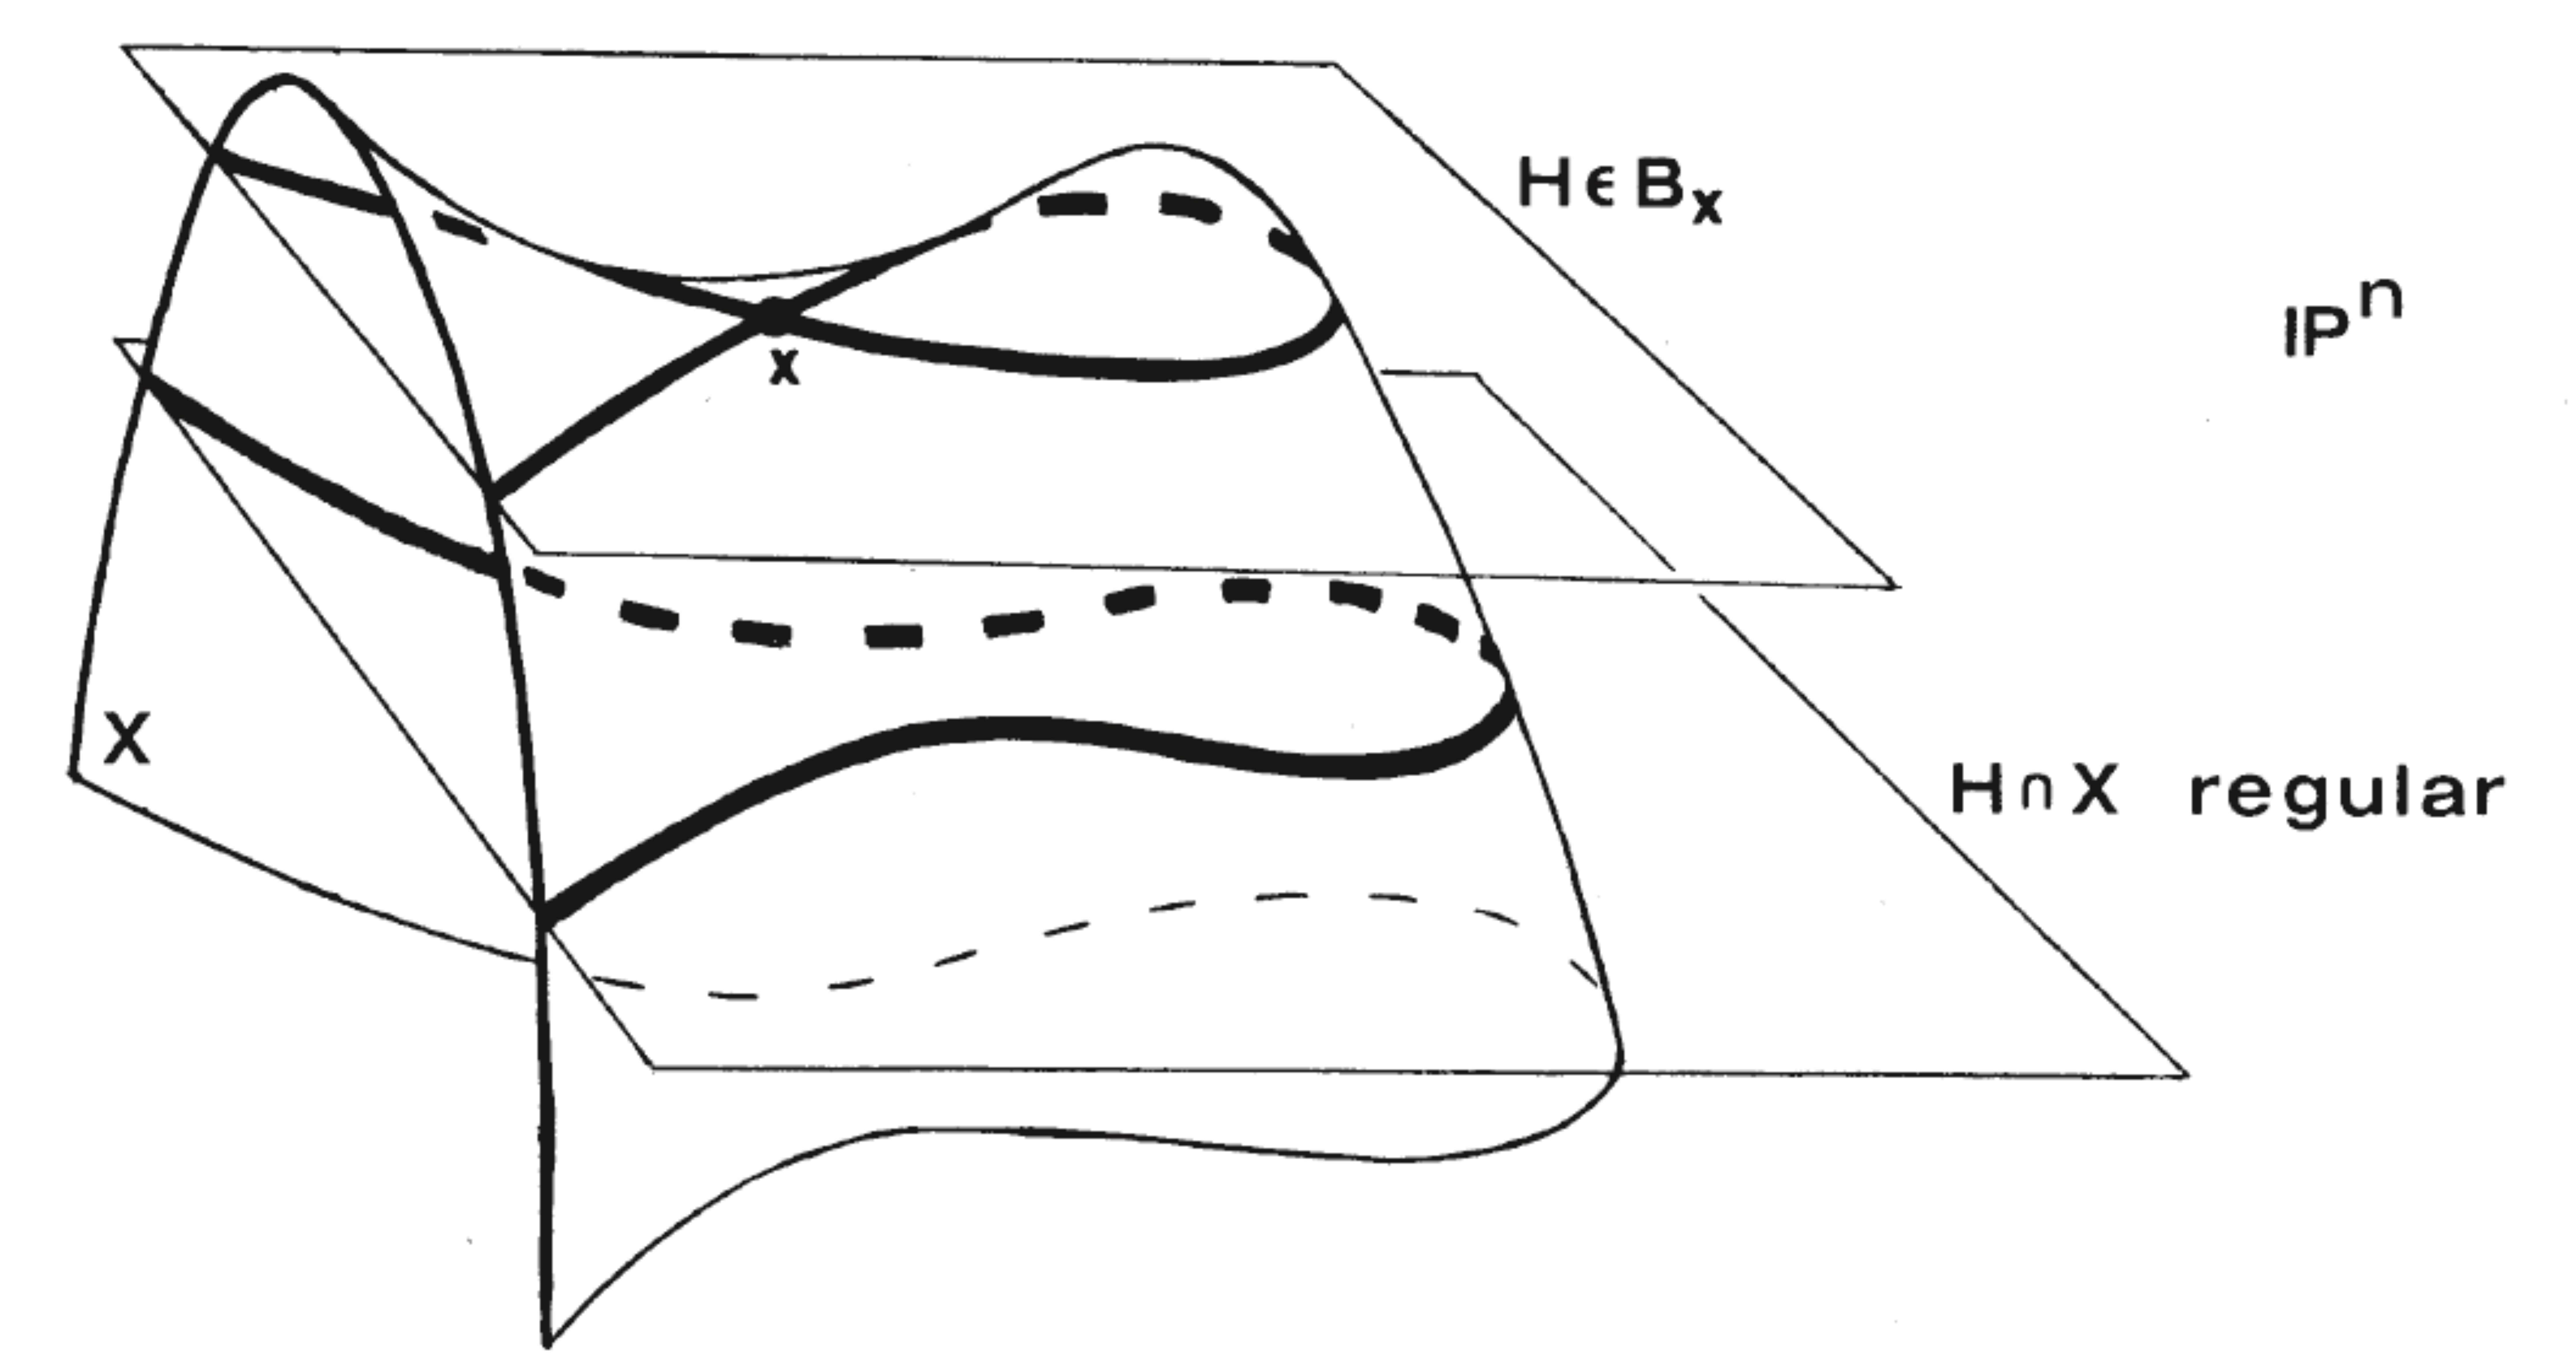
\includegraphics[width=10cm]{Figure10}\\
	Figure 10. 비특이 대수다양체의 초평면 단면
	\end{center}
	
	%
	이제 초평면 $H$가 0이 아닌 대역적 단면 $f\in V=\Ga(\Pn,\mc O_{\Pn}(1))$에 의해 결정된다.
	$x\notin H_0$인 초평면 $H_0$를 정의하는 $f_0\in V$를 고정하자. $k$-벡터 공간 사상
	%
	$$\ph_x:V\ra\mc O_{x,X}/\mf m_x^2$$
	%
	를 다음과 같이 정의할 수 있다:
	$f\in V$가 주어졌다면 $f/f_0$가 $\Pn-H_0$에서의 정칙 함수이며 이는 $X-X\cap H_0$에서의 정칙 함수를 유도한다.
	$\ph_x(f)$를 국소환 $\mc O_{x,X}$에서의 $f/f_0$의 상 법 $\mf m_x^2$로 취한다.
	이제 스킴 $H\cap X$는 $f/f_0$에 의해 생성된 $\mc O_x$의 아이디얼에 의해 $x$에서 정의된다.
	따라서 $x\in H\cap X$ iff $\ph_x(f)\in\mf m_x$이며 $x$가 $H\cap X$에서 비정칙 iff $\ph_x(f)\in\mf m_x^2$이다.
	(이 경우 $\mc O_x/(\ph(f))$가 정칙이 아니기 때문이다.)
	그러므로 우리는 초평면 $H\in B_x$들이 정확히 $f\in\ker\ph_x$들에 대응함을 알 수 있다.
	($\ph_x(f)=0\Lra H\pseq X$임도 기억해 두라.)\\
	$x$가 닫힌점이며 $k$가 대수적으로 닫혀 있으므로 $\mf m_x$는 좌표계에 대한 선형 형식들에 의해 생성되며 따라서 $\ph_x$가 전사이다.
	만약 $\dim X=r$이면 $\dim_k\mc O_x/\mf m_x^2=r+1$이다. $\dim V=n+1$이므로 $\dim\ker\ph_x=n-r$이다.
	이는 $B_x$가 (\S 7에서의 의미로) 초평면들의 차원 $n-r-1$의 선형계임을 보여준다.\\
	이제 완비선형계 $|H|$를 사영공간으로 간주하고 닫힌점 $x$와 $H\in B_x$의 모든 쌍 $\bk{x,H}$들로 구성된
	부분집합 $B\bseq X\times|H|$를 고려하자.
	명백히 $B$는 $X\times|H|$의 어떠한 닫힌 부분집합(이를 여전히 $B$로 부르고 축약 유도 부분스킴 구조를 부여하자)의 닫힌점들의 집합이다.
	우리는 첫째 사영 $p_1:B\ra X$가 전사이며 그 올이 차원 $n-r-1$의 사영공간임을 보였다.
	따라서 $B$는 기약이며 차원 $(n-r-1)+r=n-1$을 가진다.
	그러므로 둘째 사영 $p_2:B\ra|H|$를 고려하면 $\dim p_2(B)\le n-1$이다.
	$\dim|H|=n$이므로 $p_2(B)<|H|$라 결론지을 수 있다.
	만약 $H\in|H|-p_2(B)$이면 $H\not\pseq X$이며 $H\cap X$의 모든 점이 정칙이고 따라서 $H$가 정리의 요구사항을 만족시킨다.
	$X$가 사영적이므로 $p_2:X\times|H|\ra|H|$가 진 사상임을 기억해 두라;
	$B$는 $X\times|H|$에서 닫혀 있으므로 $p_2(B)$가 $|H|$에서 닫혀 있다.
	그러므로 $|H|-p_2(B)$는 $|H|$의 열린 조밀 부분집합이며 이는 정리의 마지막 진술을 증명한다.
	%
	\qed
	\end{theorem}
	
	
	%Remark 8.18.1
	\begin{remark}
	이 결과는 $X$가 유한 개 특이점을 가지더라도 여전히 성립한다.
	이들 중 임의의 점을 포함하는 초평면들의 집합은 $|H|$의 닫힌 진부분집합이기 때문이다.
	\end{remark}
	
	
	%Subsection
	\subsection*{Applications (응용)}
	%
	이제 우리는 위 발상을 체 상에서의 비특이 대수다양체의 불변량을 정의하는 데 적용할 것이다.
	
	
	%Definition
	\begin{definition}
	$X$가 $k$ 상에서의 비특이 대수다양체라 하자.
	$X$의 \tb{접층(tangent sheaf)}을 $\ms T_X=\shhom_{\mc O_X}(\Om_{X/k},\mc O_X)$로 정의한다. 이는 계수 $n=\dim X$의 국소자유층이다.
	$X$의 \tb{정준층(canonical sheaf)}을 미분의 층의 $\dim X=n$중 외멱 $\om_X=\We^n\Om_{X/k}$로 정의한다. 이는 $X$ 상에서의 가역층이다.
	만약 $X$가 사영적이며 비특이이면 $X$의 \tb{기하종수(geometric genus)}를 $p_g=\dim_k\Ga(X,\om_X)$로 정의한다. 이는 음 아닌 정수이다.
	\end{definition}
	
	
	%Remark 8.18.2
	\begin{remark}
	앞에서 (I, Ex. 7.2) 우리는 사영공간에서의 대수다양체의 산술종수 $p_a$를 정의했다.
	비특이 사영 곡선의 경우 산술종수와 기하종수가 일치한다. 이는 우리가 나중에 증명할 (III, 7.12.2) Serre 쌍대 정리의 결과이다.
	그러나 2차원 이상의 대수다양체에 대해서는 $p_a$와 $p_g$가 일치하지 않는다. (Ex. 8.3) (III, 7.12.3)도 참조하라.
	\end{remark}
	
	
	%Remark 8.18.3
	\begin{remark}
	미분의 층, 접층, 정준층이 모두 내재적으로 정의되었으므로 이들로부터 정의할 수 있는 임의의 숫자는 $X$의 동형 하에서의 불변량이다.
	우리는 이제 기하종수가 사실 비특이 사영 대수다양체의 \ti{쌍유리불변량}임을 보일 것이다.
	이는 기하종수를 분류 문제에서 극도로 중요하게 만든다.
	\end{remark}
	
	
	%Theorem 8.19
	\begin{theorem}
	$X$와 $X'$이 쌍유리동치인 $k$ 상에서의 비특이 사영 대수다양체라 하자. 그 경우 $p_g(X)=p_g(X')$이다.\\\\
	%
	\pf (I, \S 4)로부터 $X$와 $X'$이 쌍유리동치임은 $X$에서 $X'$로의 유리함수와
	$X'$에서 $X$로의 유리함수가 존재하여 서로의 역인 것임을 상기하라.
	$X$에서 $X'$으로의 유리함수를 고려하고 $V\bseq X$가 사상 $f:V\ra X'$에 의해 유리함수를 표현할 수 있는 최대 열린집합이라 하자.
	그 경우 (8.11)에 의해 함수 $f^*\Om_{X'/k}\ra\Om_{V/k}$가 존재한다.
	이들은 동일한 계수 $n=\dim X$의 국소자유층이므로 외멱 상에서의 유도된 함수 $f^*\om_{X'}\ra\om_V$를 얻는다.
	이 함수는 다시 대역적 단면의 공간에서의 함수 $f^*:\Ga(X',\om_{X'})\ra\Ga(V,\om_V)$를 유도한다.
	이제 $f$가 쌍유리이므로 (I, 4.5)에 의해 열린집합 $U\bseq V$가 존재하여
	$f(U)$가 $X'$에서 열려 있고 $f$가 $U$에서 $f(U)$로의 동형사상을 유도한다.
	그러므로 $f$를 통해 $\om_V\rest_U\cong\om_{X'}\rest_{f(U)}$이다.
	가역층의 0이 아닌 대역적 단면은 조밀 열린집합 상에서 소멸할 수 없으므로
	벡터 공간 사상 $f^*:\Ga(X',\om_{X'})\ra\Ga(V,\om_V)$가 단사여야 한다 결론지을 수 있다.\\
	다음으로 $\Ga(V,\om_V)$와 $\Ga(X,\om_X)$를 비교하자. 먼저 $X-V$가 $X$에서 여차원 2 이상임을 주장하겠다.
	이는 진성의 부치 판정법 (4.7)에서 따라온다:
	$X$의 일반점에서 $X'$으로의 함수는 이미 존재한다.
	만약 $P\in X$가 여차원 1의 점이면 ($X$가 비특이이므로) $\mc O_{P,X}$는 이산 부치환이다.
	$X'$이 사영적이며 따라서 $k$ 상에서 진이므로 유일한 사상 $\Spec\mc O_{P,X}\ra X'$이 존재하여 주어진 쌍유리함수와 호환된다.
	이는 $P$의 어떠한 근방에서 $X'$으로의 함수로 확장되며 따라서 $V$의 정의에 의해 $P\in V$여야 한다.\\
	이제 우리는 자연스러운 제한함수 $\Ga(X,\om_X)\ra\Ga(V,\om_V)$가 전단사임을 보여야 한다.
	임의의 아핀 열린 부분집합 $U\bseq X$에 대하여 $\om_X\rest_U\cong\mc O_U$이며
	$\Ga(U,\mc O_U)\ra\Ga(U\cap V,\mc O_{U\cap V})$가 전단사임을 보이면 충분하다.
	$X$가 비특이이고 따라서 정규이며 $U-U\cap V$가 $U$에서 여차원 2 이상이므로 이는 (6.3A)의 직접적인 결과이다.\\
	위 결과들을 조합하면 $p_g(X')\le p_g(X)$임을 알 수 있다. 대칭성에 의해 반대 방향 부등식이 성립하며 따라서 $p_g(X)=p_g(X')$이다.
	%
	\qed
	\end{theorem}
	
	다음으로 우리는 대수다양체 $X$의 비특이 부분대수다양체에 대한 접층과 정준층의 거동을 다룰 것이다.
	
	
	%Definition
	\begin{definition}
	$Y$가 $k$ 상에서의 비특이 대수다양체 $X$의 비특이 부분대수다양체라 하자.
	(8.17)의 국소자유층 $\ms I/\ms I^2$는 $Y$의 $X$에서의 \tb{쌍대정규층(conormal sheaf)}이다.
	그 쌍대 $\ms N_{Y/X}=\shhom_{\mc O_Y}(\ms I/\ms I^2,\mc O_Y)$는 $Y$의 $X$에서의 \tb{정규층(normal sheaf)}이다.
	이는 계수 $r=\codim(Y,X)$의 국소자유층이다.
	\end{definition}
	
	(8.17)에서 주어진 $Y$에서의 국소자유층의 완전열의 $Y$에서의 쌍대를 취하면 다음의 완전열을 얻는다.
	%
	$$0\ra\ms T_Y\ra\ms T_X\otimes\mc O_Y\ra\ms N_{Y/X}\ra 0$$
	%
	이는 방금 정의한 정규층이 정규 벡터가 주위 공간의 접벡터 법 부분공간의 접벡터라는 통상적인 기하학적 개념에 대응한다는 사실을 보여준다.
	
	
	%Proposition 8.20
	\begin{proposition}
	$Y$가 $k$ 상에서의 비특이 대수다양체 $X$에서의 여차원 $r$의 비특이 부분대수다양체라 하자.
	그 경우 $\om_Y\cong\om_X\otimes\We^r\ms N_{Y/X}$이다.
	$r=1$인 경우 $Y$를 인자로 간주하고 $\ms L$이 $X$에서의 연관된 가역층이라 하면 $\om_Y\cong\om_X\otimes\ms L\otimes\mc O_Y$이다.\\\\
	%
	\pf 다음의 완전열의 국소자유층에 최고차 외멱을 취하면,
	%
	$$0\ra\ms I/\ms I^2\ra\Om_X\otimes\mc O_Y\ra\Om_Y\ra 0$$
	%
	(Ex. 5.16d)에 의해 $\om_X\otimes\mc O_Y\cong\om_Y\otimes\We^r(\ms I/\ms I^2)$임을 알 수 있다.
	최고차 외멱을 취하는 연산이 쌍대층을 취하는 연산과 교환 가능하므로 $\om_Y\cong\om_X\otimes\We^r\ms N_{Y/X}$이다.
	$r=1$인 특수한 경우 (6.18)에 의해 $\ms I_Y\cong\ms L^{-1}$이다.
	그러므로 $\ms I/\ms I^2\cong\ms L^{-1}\otimes\mc O_Y$이며 $\ms N_{Y/X}\cong\ms L\otimes\mc O_Y$이다.
	따라서 $r=1$에 대하여 위 결과를 적용하면 $\om_Y\cong\om_X\otimes\ms L\otimes\mc O_Y$를 얻는다.
	%
	\qed
	\end{proposition}
	
	
	%Example 8.20.1
	\begin{example}
	$X=\Pn_k$라 하자. (8.13)의 완전열의 쌍대를 취하면 $\Pn$의 접층을 수반하는 다음의 완전열을 얻는다:
	%
	$$0\ra\mc O_X\ra\mc O_X(1)^{n+1}\ra\ms T_X\ra 0$$
	%
	$\Pn$ 상에서의 정준층을 얻기 위해서는 (8.13)의 완전열에 최고차 외멱을 취하면 된다. 그 경우 $\om_X\cong O_X(-n-1)$을 얻는다.
	$l<0$이면 $\mc O(l)$이 대역적 단면을 갖지 않으므로 임의의 $n\ge 1$에 대하여 $p_g(\Pn)=0$이다.
	\tb{유리 대수다양체(rational variety)}가 어떠한 $n$에 대하여 $\Pn$과 쌍유리인 대수다양체로 정의되었음을 상기하라. (I, Ex. 4.4)
	(8.19)에 의해 만약 $X$가 임의의 비특이 사영 유리 대수다양체이면 $p_g(X)=0$이라 결론지을 수 있다.
	이 사실은 모든 차원에서 비유리 대수다양체의 존재성을 보일 수 있게 해 준다.
	\end{example}
	
	
	%Example 8.20.2
	\begin{example}
	$X=\Pn_k$이며 $n\ge 2$라 하자. 임의의 정수 $d\ge 1$에 대하여 인자 $dH$($H$ 초평면)는 매우 풍부한 인자이다. (7.6.1)
	그러므로 $dH$는 적절한 사영적 매장($d$차 매장)에서의 $X$의 초평면 단면이 되며, 여기에 Bertini 정리(8.18)를 적용할 수 있다.
	그 경우 부분스킴 $Y\in|dH|$가 존재하여 모든 점에서 정칙임을 알 수 있다.
	만약 $Y$가 2개 이상의 기약 성분 $Y_1,Y_2$를 가졌다면 $n\ge 2$이므로 이들의 교집합 $Y_1\cap Y_2$가 공집합이 아니다. (I, 7.2)
	그러나 $Y_1\cap Y_2$의 임의의 점에서 $Y$가 특이이므로 우리는 $Y$가 기약이며 따라서 비특이 대수다양체라 결론지을 수 있다.
	그러므로 임의의 $d\ge 1$에 대하여 $\Pn$에서 차수 $d$인 비특이 초곡면이 존재함을 알 수 있다.
	사실 이들은 완비선형계 $|dH|$의 조밀 열린 부분집합을 형성한다. (이는 (I, Ex. 5.5)를 일반화한다.)
	\end{example}
	
	
	%Example 8.20.3
	\begin{example}
	$Y$가 $n\ge 2$인 $\Pn$에서의 $d$차 비특이 초곡면이라 하자.
	그 경우 (8.20)과 위의 첫째 예시에 의해 $\om_Y\cong\mc O_Y(d-n-1)$이라 결론지을 수 있다. 몇 가지 특수한 경우들을 살펴보자.\\
	$n=2,d=1$. $Y$는 $\mb P^2$에서의 직선이며 따라서 $Y\cong\mb P^1$이고 이미 알려진 것과 같이 $\om_Y\cong\mc O_Y(-2)$이다.\\
	$n=2,d=2$. $Y$는 $\mb P^2$에서의 원뿔곡선이며 $\om_Y\cong\mc O_Y(-1)$이다.
	이 경우 $Y$는 $\mb P^1$의 2차 매장이며 따라서 $\om_Y$를 $\mb P^1$로 당기면
	역시 이미 알려진 것과 같이 $\om_{\mb P^1}\cong\mc O_{\mb P^1}(-2)$를 얻는다.\\
	$n=2,d=3$. $Y$는 비특이 평면 3차곡선이며 $\om_Y\cong\mc O_Y$이다.
	그러므로 $p_g(Y)=\dim\Ga(Y,\mc O_Y)=1$이며 $Y$가 비유리임을 알 수 있다.
	이는 하나의 비특이 3차곡선의 예시만을 제시하고 이것이 비유리임을 다른 방법으로 보였던 (I, Ex. 6.2)를 일반화한다.
	$n=2,d\ge 4$. $Y$는 평면 비특이 $d$차곡선이며 $\om_Y\cong\mc O_Y(d-3)$이고 $d-3>0$이다.
	따라서 $p_g>0$이며 $Y$가 비유리이다.
	사실 $p_g=\fra 2(d-1)(d-2)$이며 (Ex. 8.4f) 따라서 서로 다른 차수 $d,d'\ge 3$을 가지는 평면 곡선들은 서로 쌍유리가 아니다.
	이것을 보이는 다른 방법은 다음과 같다.
	임의의 비특이 사영 곡선에 대하여 정준층의 \tb{차수(degree)}를 고려할 수 있다.
	비특이 사영 곡선은 쌍유리동치류 하에서 유일하므로 (I, \S 6) 이 수는 사실 쌍유리 불변량이다.
	이 경우 ($\mc O(1)$이 $Y$에서 차수 $d$를 가지므로) 그 값은 $d(d-3)$이다.
	이 수는 서로 다른 $d,d'\ge 3$에 대하여 다르다. 이는 무한히 많은 서로 쌍유리가 아닌 곡선들의 존재성을 보여준다.\\
	$n=3,d=1$. 이는 이미 알려진 것과 같이 $Y\cong\mb P^2,\om_Y\cong\mc O_Y(-3)$을 준다.\\
	$n=3,d=2$. 여기에서 $Y$는 비특이 2차곡면이며 $\om_Y\cong\mc O_Y(-2)$이다.
	$p_g(Y)=0$이며 이는 $Y$가 유리라는 사실과 합치한다. (I, Ex. 4.5)
	동형사상 $Y\cong\mb P^1\times\mb P^1$에 의해 $\om_Y$는 $(-2,-2)$형 인자류에 대응한다 - (6.6.1)을 참조하라.
	이는 비특이 대수다양체의 직접곱에서의 정준층이 두 인자에서의 정준층의 당김의 텐서곱이라는 일반적인 사실(Ex. 8.3)을 보여준다.\\
	$n=3,d=3$. $Y$는 $\mb P^3$에서의 비특이 3차곡면이고 $\om_Y\cong\mc O_Y(-1)$이며 따라서 $p_g(Y)=0$이다.
	이 경우 $Y$가 유리임을 나중에 (Chapter V) 보게 될 것이다.\\
	$n=3,d=4$. 이 경우 $\om_Y\cong\mc O_Y$이다. 정준층이 자명하며 따라서 $p_g=1$이다. 이는 `K3 곡면'의 족에 속하는 비유리 곡면이다.\\
	$n=3,d\ge 5$. 여기에서 $\om_Y\cong\mc O_Y(d-4)$이며 $d-4>0$이다. 따라서 $p_g>0$이며 $Y$가 비유리이다.
	정준층이 매우 풍부한 층이도록 하는 이러한 곡면은 `일반형 곡면(surfaces of general type)'의 족에 속한다.\\
	$n=4,d=3,4$. $\mb P^4$에서의 3차 및 4차 입체는 모두 $p_g=0$을 가지지만 최근에 (서로 다른 방법으로)
	이들이 일반적으로 유리 대수다양체가 아님이 밝혀졌다.
	3차 입체에 대해서는 Clemens and Griffiths [1]을, 4차 입체에 대해서는 Iskovskih and Manin [1]을 참조하라.\\
	$n$ 임의, $d\ge n+1$. 이 경우 $\Pn$에서의 비특이 초곡면 $Y$를 얻으며
	$\om_Y\cong\mc O_Y(d-n-1),d-n-1\ge 0$이다. 따라서 $p_g(Y)\ge 1$이며 $Y$가 비유리이다.
	이는 모든 차원에서의 비유리 대수다양체의 존재성을 보여준다.
	\end{example}
	
	
	%Subsection
	\subsection*{Some Local Algebra (국소대수학)}
	%
	여기에서 우리는 주로 대수기하학에서 유용한 깊이와 Cohen-Macaulay 환에 관한 국소대수학에서의 몇 가지 결과들을 모아놓을 것이다.
	그 후 우리는 이들을 국소완비교집합의 기하학적 개념과 연관시키고 부풀림에의 응용을 제시할 것이다.
	증명은 Matsumura [2, Ch. 6]을 언급할 것이다.
	
	만약 $A$가 환이며 $M$이 $A$-모듈이면 $A$의 원소들의 열 $x_1,\ldots,x_r$이 $M$에 대한 \tb{정칙열(regular sequence)}임은
	$x_1$이 $M$에서의 비영인자이며 모든 $i=2,\ldots,r$에 대하여 $x_i$가 $M/(x_1,\ldots,x_{i-1})M$에서의 비영인자인 것이다.
	만약 $A$가 극대 아이디얼 $\mf m$을 가지는 국소환이라 하면 $M$의 \tb{깊이(depth)}는
	모든 $x_i\in\mf m$인 $M$에 대한 정칙열 $x_1,\ldots,x_r$의 최대 길이이다.
	이러한 정의는 환 $A$ 자신에 대해서도 적용되며,
	Noether 국소환 $A$가 \tb{Cohen-Macaulay}라는 것의 정의는 $\depth A=\dim A$인 것이다.
	이제 우리는 Cohen-Macaulay 환의 몇 가지 성질들을 나열하겠다.
	
	
	%Theorem 8.21A
	\begin{theorema}
	$A$가 극대 아이디얼 $\mf m$을 가지는 Noether 국소환이라 하자.
	\begin{enumerate}[label=(\alph*)]
	\item 만약 $A$가 정칙이면 Cohen-Macaulay이다.
	\item 만약 $A$가 Cohen-Macaulay이면 $A$의 임의의 소 아이디얼에서의 국소화도 Cohen-Macaulay이다.
	\item 만약 $A$가 Cohen-Macaulay이면 $x_1,\ldots,x_r\in\mf m$이 $A$에 대한 정칙열을 형성할 필요충분조건은\\
	$\dim A/(x_1,\ldots,x_r)=\dim A-r$인 것이다.
	\item 만약 $A$가 Cohen-Macaulay이며 $x_1,\ldots,x_r\in\mf m$이 $A$에 대한 정칙열이면
	$A/(x_1,\ldots,x_r)$도 Cohen-Macaulay이다.
	\item 만약 $A$가 Cohen-Macaulay이며 $x_1,\ldots,x_r\in\mf m$이 정칙열이면 $I$가 아이디얼 $(x_1,\ldots,x_r)$이라 하자.
	그 경우 $t_i\mt x_i$로 정의된 자연스러운 함수 $(A/I)[t_1,\ldots,t_r]\ra\gr_IA=\Oplus_{n\ge 0}I^n/I^{n+1}$가 동형사상이다.
	다른 말로 하면 $I/I^2$가 계수 $r$의 자유 $A/I$-모듈이며 각각의 $n\ge 1$에 대하여 자연스러운 함수
	$S^n(I/I^2)\ra I^n/I^{n+1}$이 동형사상이다. (여기에서 $S^n$은 $n$중 대칭멱을 나타낸다.)\\
	\end{enumerate}
	%
	\pf Matsumura [2: (a) p. 121; (b) p. 104; (c) p. 105; (d) p/104; (e) p.110]
	\end{theorema}
	
	스킴에 대한 용어를 유지하면서 (Ex. 3.8) 우리는 Noether 환 $A$가 \tb{정규(normal)}임을
	모든 소 아이디얼 $\mf p$에 대하여 국소화 $A_{\mf p}$가 정수적으로 닫힌 정역인 것으로 정의하겠다.
	정규환은 정수적으로 닫힌 정역의 유한 개 직접곱이다.
	
	
	%Theorem 8.22A
	\begin{theorema}[Serre]
	Noether 환 $A$가 정규일 필요충분조건은 다음 두 조건을 만족시키는 것이다:\\
	%
	\begin{enumerate}[label=(\arabic*)]
	\item 높이 1 이하의 모든 소 아이디얼 $\mf p\bseq A$에 대하여 $A_{\mf p}$가 정칙이다. (따라서 체 또는 정칙 국소환이다.)
	\item 높이 2 이상의 모든 소 아이디얼 $\mf p\bseq A$에 대하여 $\depth A_{\mf p}\ge 2$이다.\\
	\end{enumerate}
	%
	\pf Matsumura [2, Th. 39, p.125]. 조건 (1)은 때로는 `$R_1$' 또는 `여차원 1에서 정칙'이라 불린다.
	조건 (2)는 $\height\mf p=1$이면 $\depth A_{\mf p}=1$이라는 요구조건 하에서 (1)의 결과이다.
	이는 `Serre의 $S_2$ 조건'이라 불린다.
	\end{theorema}
	
	이제 우리는 이 결과들을 대수기하학에 적용할 것이다. 스킴이 \tb{Cohen-Macaulay}임을 모든 국소환이 Cohen-Macaulay인 것으로 정의한다.
	
	
	%Definition
	\begin{definition}
	$Y$가 $k$ 상에서의 비특이 대수다양체 $X$의 닫힌 부분스킴이라 하자.
	$Y$가 $X$에서의 \tb{국소완비교집합(local complete intersection)}임을
	$Y$의 $X$에서의 아이디얼 층 $\ms I_Y$가 모든 점에서 국소적으로 $r=\codim(Y,X)$개 원소에 의해 생성될 수 있는 것으로 정의한다.
	\end{definition}
	
	
	%Example 8.22.1
	\begin{example}
	만약 $Y$ 자신이 비특이이면 (8.17)에 의해 이는 이를 포함하는 임의의 비특이 $X$ 내에서 국소완비교집합이다.
	\end{example}
	
	
	%Remark 8.22.2
	\begin{remark}
	국소완비교집합의 개념은 사실 스킴 $Y$의 내재적 성질이다. i.e. 이를 포함하는 비특이 대수다양체에 독립적이다.
	이는 위에서 도입된 상대적 미분의 개념을 확장하는 사상의 여접복합체(cotangent complex)의 개념을 사용하여 증명되었다 -
	Lichtenbaum and Schlessinger [1]을 참조하라. 우리는 이 사실을 과정 중에서 사용하지 않을 것이다.
	\end{remark}
	
	
	%Proposition 8.23
	\begin{proposition}
	$Y$가 $k$ 상에서의 비특이 대수다양체 $X$의 국소완비교집합 부분스킴이라 하자. 그 경우 다음이 성립한다:
	%
	\begin{enumerate}[label=(\alph*)]
	\item $Y$가 Cohen-Macaulay이다.
	\item $Y$가 정규일 필요충분조건은 여차원 1에서 정칙인 것이다.\\
	\end{enumerate}
	%
	\pf (a) $X$가 비특이이면 (8.21Aa)에 의해 이는 Cohen-Macaulay이다.
	$\ms I_Y$가 국소적으로 $r=\codim(Y,X)$개 원소들에 의해 생성되므로
	(8.21Ac)에 의해 이러한 원소들은 국소적으로 $\mc O_X$에서의 정칙열을 형성한다.
	그러므로 (8.21Ad)에 의해 $Y$가 Cohen-Macaulay이다.\\
	(b) 우리는 이미 정규가 여차원 1에서 정칙임을 함의함을 알고 있다. (I, 6.2A)
	역을 위해서는 (8.22A)를  $Y$의 국소환들에 적용해야 한다.
	조건 (1)은 우리의 전제조건이며 (2)는 $Y$가 Cohen-Macaulay이므로 자동적으로 성립한다.
	%
	\qed
	\end{proposition}
	
	마지막 응용으로 우리는 비특이 대수다양체의 비특이 부분대수다양체에서의 부풀림을 고려할 것이다. (부풀림의 정의를 위해서는 \S 7을 참조하라.)
	다음 정리는 $X$와 $\tilde X$의 불변량을 비교하는 데 유용할 것이다. (Ex. 8.5)
	
	
	%Theorem 8.24
	\begin{theorem}
	$X$가 $k$ 상에서의 비특이 대수다양체이며 $Y\bseq X$가 비특이 닫힌 부분대수다양체이고 아이디얼 층 $\ms I$를 가진다 하자.
	$\pi:\tilde X\ra X$가 $\ms I$의 부풀림이며 $Y'\bseq\tilde X$가
	역상 아이디얼 층 $\ms I'=\pi^{-1}\ms I\cdot\mc O_{\tilde X}$에 의해 정의된 부분스킴이라 하자. 그 경우 다음이 성립한다:
	%
	\begin{enumerate}[label=(\alph*)]
	\item $\tilde X$도 비특이이다.
	\item $Y'$와 유도된 사영사상 $\pi:Y'\ra Y$의 쌍은 $Y$ 상에서의 (국소자유)층
	$\ms I/\ms I^2$에 연관된 사영공간다발 $\mb P(\ms I/\ms I^2)$와 동형이다.
	\item 이러한 동형사상 하에서 정규층 $\ms N_{Y'/\tilde X}$는 $\mc O_{\mb P(\ms I/\ms I^2)}(-1)$에 대응한다.\\
	\end{enumerate}
	%
	\pf 먼저 (b)를 증명한다. $\tilde X=\bProj\Oplus\ms I^d$이므로 다음이 성립한다.
	%
	$$Y'\cong\bProj\Oplus(\ms I^d\otimes\mc O_X/\ms I)=\bProj\Oplus\ms I^d/\ms I^{d+1}$$
	%
	그러나 $Y$가 비특이이므로 $\ms I$는 국소적으로 $\mc O_X$에서의 정칙열에 의해 생성되며 (8.21Ae)를 적용 가능하다.
	이는 $\ms I/\ms I^2$가 국소자유이며 각각의 $n\ge 1$에 대하여 $\ms I^n/\ms I^{n+1}\cong S^n(\ms I/\ms I^2)$임을 함의한다.
	그러므로 $Y'\cong\bProj\Oplus S^n(\ms I/\ms I^2)$이며 이는 정의에 의해 $\mb P(\ms I/\ms I^2)$이다.\\
	특히 $r=\codim(Y,X)$라 하면 $Y'$은 $Y\times\mb P^{r-1}$과 국소적으로 동형이며 따라서 $Y'$도 비특이이다.
	$Y'$이 $\tilde X$에서 국소주이므로 (7.13a) $\tilde X$도 비특이임이 따라온다:
	만약 Noether 국소환의 비영인자에 의한 몫이 정칙이면 원래 국소환도 정칙이다.\\
	(c)를 증명하기 위해 (7.13)의 증명에서 $\ms I'=\pi^{-1}(\ms I)\cdot\mc O_{\tilde X}$가 $\mc O_{\tilde X}(1)$과 동형임을 상기하라.
	$\ms I'/\ms I'^2\cong\mc O_{Y'}(1)$이며 따라서 $\ms N_{Y'/\tilde X}\cong\mc O_{Y'}(-1)$임이 따라온다.
	%
	\qed
	\end{theorem}
	
	다음의 대수적 결과를 연습문제에서 사용할 것이다.
	
	%Theorem 8.25A.
	\begin{theorema}[I. S. Cohen]
	$A$가 체 $k$를 포함하는 완비 국소환이라 하자. 잉여류체 $k(A)=A/\mf m$이 $k$의 가분생성 확대라 하자.
	그 경우 부분체 $K\bseq A$가 존재하여 $k$를 포함하며 $K\ra A/\mf m$이 동형사상이도록 한다.
	(부분체 $K$는 $A$에 대한 \tb{대표원체(field of representatives)}라 불린다.)\\\\
	%
	\pf Matsumura [2, p. 105]
	\end{theorema}
	
	
	
	%Exercises
	\subsection*{Exercises (연습문제)}
	
	\begin{enumerate}[label=\tb{8.\arabic*.},itemindent=0mm,itemsep=2mm]
	\item 여기에서 우리는 스킴 $X$의 닫혀 있을 필요는 없는 점에서의 미분의 층에 대한 정보를 포함하도록 본문의 결과들을 강화할 것이다.
	\begin{enumerate}[label=(\alph*)]
	\item (8.7)을 다음과 같이 일반화하라. $B$가 체 $k$를 포함하는 국소환이며 $B$의 잉여류체 $k(B)=B/\mf m$이 $k$의 가분생성 확대라 하자.
	그 경우 (8.4A)의 완전열은 좌측에서도 완전하다.
	%
	$$0\ra\mf m/\mf m^2\sr\de\ra\Om_{B/k}\otimes k(B)\ra\Om_{k(B)k}\ra 0$$
	%
	[Hint: (8.7)의 증명을 복사하여 먼저 완비 국소환 $B/\mf m^2$를 통과하고 $B/\mf m^2$에 대한 대표원체를 선택하기 위해 (8.25A)를 사용하라.]
	\item (8.8)을 다음과 같이 일반화하라. 위와 같은 $B,k$에 대하여 추가적으로 $k$가 완전체이며
	$B$가 $k$ 상에서의 유한형 대수의 국소화라 가정하자.
	그 경우 $B$가 정칙 국소환일 필요충분조건은 $\Om_{B/k}$가 계수 $\dim B+\trd k(B)/k$의 자유 모듈인 것이다.
	\item (8.15)를 다음과 같이 강화하라. $X$가 완전체 $k$ 상에서의 유한형 기약 스킴이며 $\dim X=n$이라 하자.
	(닫혀 있을 필요는 없는) 임의의 점 $x\in X$에 대하여 국소환 $\mc O_{x,X}$가 정칙 국소환일 필요충분조건은
	미분의 층의 $x$에서의 줄기 $(\Om_{X/k})_x$가 계수 $n$의 자유 모듈인 것이다.
	\item (8.16)을 다음과 같이 강화하라. 만약 $X$가 대수적으로 닫힌 체 $k$ 상에서의 대수다양체이면
	$U=\sx{x\in X}{\mc O_x\text{가 정칙 국소환}}$는 $X$의 조밀 열린 부분집합이다.
	\end{enumerate}
	\item $X$가 $k$ 상에서의 $n$차원 대수다양체라 하자. $\ms E$가 $X$에서의 계수 $n$ 초과의 국소자유층이라 하고
	$V\bseq\Ga(X,\ms E)$가 $\ms E$를 생성하는 대역적 단면들의 벡터 공간이라 하자.
	원소 $s\in V$가 존재하여 각각의 $x\in X$에 대하여 $s_x\notin\mf m_x\ms E_x$를 만족시킴을 보여라.
	다음 완전열을 만족시키는 사상 $\mc O_X\ra\ms E$가 존재한다 결론지어라.
	%
	$$0\ra\mc O_X\ra\ms E\ra\ms E'\ra 0$$
	%
	여기에서 $\ms E'$도 국소자유층이다. [Hint: Bertini 정리(8.18)의 증명과 유사한 방법을 사용하라.]
	\item \tb{곱 스킴.}
	\begin{enumerate}[label=(\alph*)]
	\item $X$와 $Y$가 다른 스킴 $S$ 상에서의 스킴이라 하자.
	(8.10)과 (8.11)을 사용하여 $\Om_{X\times_SY/S}\cong p_1^*\Om_{X/S}\oplus p_2^*\Om_{Y/S}$임을 보여라.
	\item 만약 $X$와 $Y$가 체 $k$ 상에서의 비특이 대수다양체이면 $\om_{X\times Y}\cong p_1^*\om_X\otimes p_2^*\om_Y$임을 보여라.
	\item $Y$가 비특이 평면 3차곡선이며 $X$가 곡면 $Y\times Y$라 하자. $p_g(X)=1$이지만 $p_a(X)=-1$임을 보여라. (I, Ex. 7.2)
	이는 비특이 사영 대수다양체의 산술종수와 기하종수가 다를 수 있음을 보여준다.
	\end{enumerate}
	\item \tb{$\Pn$에서의 완비교집합.} $\Pn_k$의 닫힌 부분스킴 $Y$가
	\tb{(엄격한, 대역적) 완비 교집합((strict, global) complete intersection)}이라는 것의 정의는 
	$Y$의 $S=k[x_0,\ldots,x_n]$에서의 동차 아이디얼 $I$가 $r=\codim(Y,\Pn)$개 원소들에 의해 생성될 수 있는 것이다. (I, Ex. 2.17)
	\begin{enumerate}[label=(\alph*)]
	\item $Y$가 $\Pn$에서의 여차원 $r$의 닫힌 부분스킴이라 하자.
	그 경우 $Y$가 완비 교집합일 필요충분조건은 초곡면(i.e. 여차원 1의 국소주 부분스킴) $H_1,\ldots,H_r$이 존재하여
	\ti{스킴으로서} $Y=H_1\cap\cdots\cap H_r$인 것이다. i.e. $\ms I_Y=\ms I_{H_1}+\cdots+\ms I_{H_r}$.
	[Hint: $S$에서 비혼합성 정리(unmixedness theorem; Matsumura [2, p. 107])가 성립한다는 사실을 사용하라.]
	\item 만약 $Y$가 $\Pn$에서의 1차원 이상의 완비 교집합이며 $Y$가 정규이면 $Y$는 사영적 정규이다. (Ex. 5.14)
	[Hint: (8.23)을 $Y$ 상에서의 아핀 원뿔에 적용하라.]
	\item (b)와 동일한 전제조건 하에서 모든 $l\ge 0$에 대하여 자연스러운 함수 $\Ga(\Pn,\mc O_{\Pn}(l))\ra\Ga(Y,\mc O_Y(l))$가 전사이다.
	특히 $l=0$으로 선택하여 $Y$가 연결임을 보여라.
	\item 정수 $d_1,\ldots,d_r\ge 1,r<n$이 주어졌다 하자. Bertini 정리(8.18)를 사용하여
	$\Pn$에서의 비특이 초곡면 $H_1,\ldots,H_r$이 존재하여 $\deg H_i=d_i$이며
	스킴 $Y=H_1\cap\cdots\cap H_r$이 기약이며 비특이이고 $\Pn$에서 여차원 $r$임을 보여라.
	\item 만약 $Y$가 (d)에서와 같은 비특이 완비교집합이면 $\om_Y\cong\mc O_Y(\sum d_i-n-1)$임을 보여라.
	\item 만약 $Y$가 $\Pn$에서의 비특이 $d$차초곡면이면 (c)와 (e)를 사용하여 $p_g(Y)=\binom{d-1}n$임을 보여라.
	그러므로 $p_g(Y)=p_a(Y)$이다. (I, Ex. 7.2)
	특히 만약 $Y$가 평면 $d$차곡선이면 $p_g(Y)=\fra 2(d-1)(d-2)$이다.
	\item 만약 $Y$가 $\mb P^3$에서의 비특이 곡선이며 차수 $d,e$의 비특이 곡면들의 완비교집합이면 $p_g(Y)=\fra 2de(d+e-4)+1$이다.
	다시 기하종수는 산술종수와 같다. (I, Ex. 7.2)
	\end{enumerate}
	\item \tb{비특이 대수다양체의 부풀림.} (8.24)에서와 같이 $X$가 비특이 대수다양체이고 $Y$가 여차원 $r\ge 2$의 비특이 부분대수다양체이며
	$\pi:\tilde X\ra X$가 $X$의 $Y$에서의 부풀림이며 $Y'=\pi^{-1}(Y)$라 하자.
	\begin{enumerate}[label=(\alph*)]
	\item 함수 $\pi^*:\Pic X\ra\Pic\tilde X$와 $n\mt nY'$의 인자류로 정의된 $\Z\ra\Pic X$가
	동형사상 $\Pic\tilde X\cong\Pic X\oplus\Z$를 제공한다.
	\item $\om_{\tilde X}\cong f^*\om_X\otimes\ms L((r-1)Y')$임을 보여라.
	[Hint: (a)에 의해 우리는 항상 $X$에서의 어떠한 가역층 $\ms M$와 어떠한 정수 $q$에 대하여
	$\om_{\tilde X}\cong f^*\ms M\otimes\ms L(qY')$으로 표현 가능하다.
	$\tilde X-Y'\cong X-Y$로 제한하는 것으로 $\ms M\cong\om_X$임을 보여라. $q$를 결정하기 위해 다음과 같이 진행하라:
	먼저 $\om_{Y'}\cong f^*\om_X\otimes\mc O_{Y'}(-q-1)$임을 보여라.
	그 후 닫힌점 $y\in Y$를 취하고 $Z$가 $Y'$의 $y$ 상에서의 올이라 하자.
	그리고 $\om_Z\cong\mc O_Z(-q-1)$임을 보여라. 그러나 $Z\cong\mb P^{r-1}$이므로 $\om_Z\cong\mc O_Z(-r)$이며 따라서 $q=r-1$이다.]
	\end{enumerate}
	\item \tb{무한소 올림 성질.} 다음 결과는 비특이 대수다양체의 변형을 연구하는 데 매우 중요하다.
	$k$가 대수적으로 닫힌 체이고 $A$가 유한생성 $k$-대수이며 $\Spec A$가 $k$ 상에서의 비특이 대수다양체라 하자.
	$B'$이 $k$-대수이고 $I$가 $I^2=0$인 아이디얼이며 $0\ra I\ra B'\ra B\ra 0$이 완전열이라 하자.
	마지막으로 $k$-대수 준동형사상 $f:A\ra B$가 주어졌다 하자. $k$-대수 준동형사상 $g:A\ra B'$이 존재하여 다음 가환 도표를 만족시킨다.
	%
	$$\begin{tikzcd}[row sep=small,column sep=large ]&0\arrow[d]\\&I\arrow[d]\\&B'\arrow[d]\\
	A\arrow[dashed,ur,"g"]\arrow[r,swap,"f"]&B\arrow[d]\\&0\end{tikzcd}$$
	%
	우리는 이 결과를 $A$에 대한 \tb{무한소 올림 성질(infinitesimal lifting property)}이라 한다. 이 결과를 여러 단계를 거쳐 증명하겠다.
	\begin{enumerate}[label=(\alph*)]
	\item 먼저 $f$의 준동형사상 올림 $g:A\ra B'$이 주어졌다 하자.
	만약 $g':A\ra B'$이 다른 준동형사상 올림이면 $\ta=g-g'$이 $A$에서 $I$로의 $k$-미분작용소이며
	이를 $\Hom_A(\Om_{A/k},I)$의 원소로 간주할 수 있다.
	$I^2=0$이므로 $I$가 자연스러운 $B$-모듈 구조를 가지며 따라서 $A$-모듈 구조를 가진다.
	역으로 임의의 $\ta\in\Hom_A(\Om_{A/k},I)$에 대하여 $g'=g+\ta$는 $f$의 다른 준동형사상 올림이다.
	(이 단계에서는 $\Spec A$가 비특이라는 전제조건이 필요하지 않다.)
	\item 이제 $P=k[x_1,\ldots,x_n]$이 $k$ 상에서의 다항식환이며 $A$가 $P$의 핵 $J$에 대한 몫이라 하자.
	준동형사상 $h:P\ra B'$이 존재하여 다음 가환 도표를 만족시킴을 보여라.
	%
	$$\begin{tikzcd}[row sep=small,column sep=large]
	0\arrow[d]&0\arrow[d]\\J\arrow[d]&I\arrow[d]\\P\arrow[d]\arrow[r,"h"]&B'\arrow[d]\\
	A\arrow[d]\arrow[r,"f"]&B\arrow[d]\\0&0\end{tikzcd}$$
	%
	또한 $h$가 $A$-선형 사상 $\bar h:J/J^2\ra I$를 유도함을 보여라.
	\item 이제 $\Spec A$가 비특이라는 전제조건과 (8.17)을 사용하여 다음의 완전열을 얻어라.
	%
	$$0\ra J/J^2\ra\Om_{P/k}\otimes A\ra\Om_{A/k}\ra 0$$
	%
	추가적으로 함자 $\Hom_A(\cdot,I)$를 적용하면 다음 완전열을 얻음을 보여라.
	%
	$$0\ra\Hom_A(\Om_{A/k},I)\ra\Hom_P(\Om_{P/k},I)\ra\Hom_A(J/J^2,I)\ra 0$$
	%
	$\ta\in\Hom_P(\Om_{P/k},I)$가 상이 $\bar h\in\Hom_A(J/J^2,I)$를 주는 원소라 하자.
	$\ta$를 $P$에서 $B'$으로의 미분작용소로 간주하자. 그 후 $h'=h-\ta$라 하고 $h'$이 $h'(J)=0$을 만족시키는 준동형사상 $P\ra B'$임을 보여라.
	그러므로 $h'$은 요구된 준동형사상 $g:A\ra B'$을 유도한다.
	\end{enumerate}
	\item 무한소 올림 성질의 응용으로 다음의 일반적인 문제를 고려한다.
	$X$가 $k$ 상에서의 유한형 스킴이며 $\ms F$가 $X$ 상에서의 연접층이라 하자.
	우리는 다음을 만족시키는 $k$ 상에서의 스킴 $X'$을 분류하고자 한다:
	아이디얼의 층 $\ms I$가 존재하여 $\ms I^2=0$이며 $(X',\mc O_{X'}/\ms I)\cong(X,\mc O_X)$이고
	여기에 의해 주어진 $\mc O_X$-모듈 구조를 가지는 $\ms I$가 주어진 층 $\ms F$와 동형이다.
	이러한 쌍 $X',\ms I$를 스킴 $X$의 층 $\ms F$에 의한 \tb{무한소 확대(infinitesimal extension)}이라 한다.
	이러한 확대 중 한 가지인 \ti{자명한} 확대는 다음과 같이 얻을 수 있다:
	가환군의 층으로서 $\mc O_{X'}=\mc O_X\oplus\ms F$로 선택하고 곱셈을 $(a\oplus f)\cdot(a'\oplus f')=aa'\oplus(af'+a'f)$로 정의한다.
	그 경우 위상공간 $X$에 환의 층 $\mc O_{X'}$을 부여한 것은 $X$의 $\ms F$에 의한 무한소 확대이다.\\
	$X$의 $\ms F$에 의한 확대들을 분류하는 일반적인 문제는 상당히 복잡하다. 그러므로 지금은 특수한 경우만을 증명하라:
	만약 $X$가 아핀이며 비특이이면 $X$의 연접층 $\ms F$에 의한 임의의 확대는 자명한 확대와 동형이다.
	다른 경우를 위해서는 (III, Ex. 4.10)을 참조하라.
	\item $X$가 $k$ 상에서의 비특이 사영 대수다양체라 하자. 임의의 $n>0$에 대하여 $X$의 \tb{$n$번째 다중종수($n$th plurigenus)}를
	$P_n=\dim_k\Ga(X,\om_X^{\otimes n})$으로 정의한다. 그러므로 특히 $P_1=p_g$이다.
	또한 $0\le q\le\dim X$인 모든 $q$에 대하여 정수 $h^{q,0}=\dim_k\Ga(X,\Om^q_{X/k})$로 정의한다.
	여기에서 $\Om^q_{X/k}=\We^q\Om_{X/k}$는 $X$에서의 정칙 $q$-형식들의 층이다.
	특히 $q=\dim X$인 경우에는 다시 기하종수가 된다. 정수 $h^{q,0}$들은 \tb{Hodge 수(Hodge number)}라 불린다.\\
	(8.19)의 방법을 사용하여 $P_n$과 $h^{q,0}$가 $X$의 \ti{쌍유리}불변량임을 보여라.
	i.e. 만약 $X$와 $X'$이 쌍유리동치 비특이 사영 대수다양체이면 $P_n(X)=P_n(X')$이며 $h^{q,0}(X)=h^{q,0}(X')$이다.
	\end{enumerate}
	
	
	
	%Section 9
	\section{Formal Scheme (형식적 스킴)}
	%
	스킴 이론과 더 오래된 대수다양체 이론을 명확히 구별하는 한 가지 특성은 스킴의 구조층이 멱영원을 가질 가능성이다.
	특히 만약 $Y$가 대수다양체 $X$의 아이디얼 층 $\ms I$에 의해 정의된 닫힌 부분대수다양체이면
	임의의 $n\ge 1$에 대하여 아이디얼 층 $\ms I$의 $n$중멱 $\ms I^n$에 의해 정의된 닫힌 부분스킴 $Y_n$을 고려할 수 있다.
	$n\ge 2$에 대하여 이는 멱영원을 가지는 스킴이다. 이는 $Y$와 $Y$에서 $X$로의 매장의 무한소 선질에 대한 정보를 동시에 가지고 있다.
	
	아래에서 엄밀하게 정의될 $Y$의 $X$에서의 형식적 완비화는 $Y$의 모든 무한소 근방 $Y_n$들에 대한 정보를 동시에 포함한다.
	그러므로 이는 어떠한 $Y_n$보다도 더 두껍지만 이는 $Y$의 $X$에서의 임의의 실제 열린 근방 내에 포함된다.
	우리는 이를 $Y$의 $X$에서의 형식적 근방이라 부를 것이다.
	
	이러한 형식적 완비화는 Zariski의 자서전 [3]에도 암시적으로 나타나 있다.
	여기에서 그는 연결성 원리의 증명에서 `부분대수다양체를 따른 홀로모픽 함수'를 사용한다.
	우리는 (III, \S 11)에서 코호몰로지를 사용하여 Zariski의 결과들 중 일부에 대한 다른 증명을 제시할 것이다.
	부분대수다양체와 주위 대수다양체 사이의 무언가로서의 형식적 스킴의 충격적인 응용은
	$\Pic$와 $\pi_1$에 대한 Lefschetz 정리에 대한 Grothendieck의 증명에서 찾아볼 수 있다. [SGA 2]
	이 내용은 Hartshorne [5, Ch. IV]에도 설명되어 있다.
	
	우리는 임의의 형식적 스킴을 국소적으로 통상적인 스킴의 닫힌 부분스킴에서의 완비화처럼 보이는 무언가로 정의할 것이다.
	
	
	%Subsection
	\subsection*{Inverse Limits of Abelian Groups (가환군의 역극한)}
	%
	먼저 역극한의 개념을 상기하자. 가환군의 \tb{역계(inverse system)}는 가환군 $A_n\;(n\ge 1)$의 족에
	준동형사상 $\ph_{n'n}:A_{n'}\ra A_n\;(n'\ge n)$이 추가된 것이며
	각각의 $n''\ge n'\ge n$에 대하여 $\ph_{n''n}=\ph_{n'n}\circ\ph_{n''n'}$을 만족시키는 것이다.
	역계를 $(A_n,\ph_{n'n})$, 또는 $\ph$가 알려진 경우 간단히 $(A_n)$으로 표기할 것이다.
	만약 $(A_n)$이 가환군의 역계이면 \tb{역극한(inverse limit)} $A=\limla A_n$을
	모든 $n'\ge n$에 대하여 $\ph_{n'n}(a_{n'})=a_n$을 만족시키는 점렬 $\{a_n\}\in\prod A_n$들의 집합으로 정의한다.
	명백히 $A$는 군이다. 역극한 $A$는 다음의 보편 성질에 의해 특성화될 수 있다:
	군 $B$와 각각의 $n$에 대한 준동형사상 $\psi_n:B\ra A_n$이 주어져
	각각의 $n'\ge n$에 대하여 $\psi_n=\ph_{n'n}\circ\psi_{n'}$을 만족시킬 경우
	유일한 준동형사상 $\psi:B\ra A$가 존재하여 각각의 $n$에 대하여 $\psi_n=p_n\circ\psi$를 만족시킨다.
	(여기에서 $p_n:A\ra A_n$은 $n$번째 사영 $\prod A_n\ra A_n$의 제한이다.)
	
	군 $A_n$이 체 $k$ 상에서의 벡터 공간 또는 환 $R$ 상에서의 모듈 등의 추가적인 구조를 가질 경우
	위 논의는 $k$-벡터 공간 또는 $R$-모듈의 범주에서 유효하다.\\
	
	다음으로 우리는 역극한의 완전성 성질을 다룰 것이다. (cf. Atiyah-Macdonald [1, Ch. 10])
	가환군의 역계의 \tb{준동형사상(homomorphism)} $(A_n)\ra(B_n)$은
	역계의 함수들과 호환 가능한 각각의 $n$에 대한 준동형사상 $f_n:A_n\ra B_n$들의 족이다.
	i.e. 각각의 $n'\ge n$에 대하여 다음의 가환 도표가 성립한다.
	%
	$$\begin{tikzcd}[column sep=large,row sep=large]
	A_{n'}\arrow[r,"f_{n'}"]\arrow[d,"\ph_{n'n}"]&B_{n'}\arrow[d,"\psi_{n'n}"]\\A_n\arrow[r,"f_n"]&B_{n'}\end{tikzcd}$$
	%
	역계의 준동형사상의 열
	%
	$$0\ra(A_n)\ra(B_n)\ra(C_n)\ra 0$$
	%
	가 \tb{완전(exact)}열이라는 것의 정의는 각각의 $n$에 대하여 대응하는 군의 열이 완전열인 것이다.
	이러한 역계의 짧은 완전열이 주어진 경우 다음과 같은 역극한들의 열도 완전열임을 간단히 보일 수 있다.
	%
	$$0\ra\limla A_n\ra\limla B_n\ra\limla C_n$$
	%
	그러나 마지막 함수는 전사일 필요가 없다. 그러므로 $\limla$는 좌 완전 함자이다.\\
	$\limla$의 우측에서의 완전성에 대한 판정법을 제시하기 위해 우리는 다음을 정의한다:
	역계 $(A_n,\ph_{n'n})$이 \tb{Mittag-Leffler 조건(Mittag-Leffler condition)}(ML)을 만족시킨다는 것의 정의는
	각각의 $n$에 대하여 $A_n$의 부분군들의 감소 족 $\sx{\ph_{n'n}(A_n)\bseq A_n}{n'\ge n}$가 안정한 것이다.
	다르게 표현하면 각각의 $n$에 대하여 어떠한 $n_0\ge n$이 존재하여 모든 $n',n''\ge n_0$에 대하여
	$A_n$의 부분군으로서 $\ph_{n'n}(A_{n'})=\ph_{n''n}(A_{n''})$이도록 한다.
	
	역계 $(A_n)$이 (ML)을 만족시킨다 하자. 그 경우 각각의 $n$에 대하여 $A_n'\bseq A_n$이
	임의의 $n'\ge n_0$에 대한 \tb{안정상(stable image)} $\ph_{n'n}(A_{n'})$이라 하자. 이는 정의에 의해 존재한다.
	그 경우 $(A_n')$도 유도된 함수들을 가지는 역계이며 새로운 역계 $(A_n')$의 함수들은 모두 전사임을 알 수 있다.
	이에 더해 $\limla A_n'=\limla A_n$임은 명백하다. 따라서 $A=\limla A_n$은 자연스러운 함수에 의해 각각의 $A_n'$으로 전사 대응된다.
	
	
	%Proposition 9.1
	\begin{proposition}
	다음이 가환군의 역계의 짧은 완전열이라 하자.
	%
	$$0\ra(A_n)\sr f\ra(B_n)\sr g\ra(C_n)\ra0$$
	%
	그 경우 다음이 성립한다:
	%
	\begin{enumerate}[label=(\alph*)]
	\item 만약 $(B_n)$이 (ML)을 만족시키면 $(C_n)$도 그러하다.
	\item 만약 $(A_n)$이 (ML)을 만족시키면 다음의 역극한의 열도 완전열이다.
	%
	$$0\ra\limla A_n\ra\limla B_n\ra\limla C_n\ra 0$$
	%
	\end{enumerate}
	\pf (Grothendieck [EGA $0_{\mrm{III}}$, 13.2]도 참조하라.)\\
	(a) 각각의 $n'\ge n$에 대하여 $B_{n'}$의 $B_n$에서의 상은 $C_{n'}$의 $C_n$에서의 상으로 전사 대응되며
	따라서 $(B_n)$에 대한 (ML)이 $C_n$에 대한 (ML)을 즉시 함의한다.\\
	(b) 유일하게 자명하지 않은 부분은 마지막 함수가 전사임을 보이는 것이다. 그러므로 $\{c_n\}\in\limla C_n$이라 하자.
	각각의 $n$에 대하여 $E_n=g^{-1}(c_n)$이라 하자. 그 경우 $E_n$은 $B_n$의 부분집합이며 $(E_n)$은 집합의 역계이다.
	이에 더해 $0\ra A_n\ra B_n\ra C_n\ra 0$이 완전열이므로 각각의 $E_n$은 (유일하지 않은 방식으로) $A_n$과 전단사 대응된다.
	$(A_n)$이 (ML)을 만족시키므로 $(E_n)$이 집합의 역계로서 Mittag-Leffler 조건(동일하게 정의됨)을 만족시킴을 간단히 보일 수 있다.
	각각의 $E_n$이 공집합이 아니므로 위에서와 같이 안정상들의 역계를 고려하는 것으로 $\limla E_n$도 공집합이 아님이 따라온다.
	이 집합의 임의의 원소를 선택하면 $\{c_n\}$으로 대응되는 $\limla B_n$의 원소를 얻는다.
	%
	\qed
	\end{proposition}
	
	
	%Example 9.1.1
	\begin{example}
	만약 모든 함수 $\ph_{n'n}:A_{n'}\ra A_n$이 전사이면 $(A_n)$은 (ML)을 만족시키며 따라서 (9.1b)를 적용 가능하다.
	\end{example}
	
	
	%Example 9.1.2
	\begin{example}
	만약 $(A_n)$이 체 상에서의 유한 차원 벡터 공간의 역계이면,
	또는 더 일반적으로 환 상에서의 하강 연쇄 조건(DCC)을 만족시키는 모듈들의 역계이면 $(A_n)$이 (ML)을 만족시킨다.
	\end{example}
	
	
	%Subsection
	\subsection*{Inverse Limits of Sheaves (층의 역극한)}
	
	임의의 범주 $\mf C$에서 역극한의 개념을 위에서의 가환군의 역극한의 보편 성질과 유사한 방식으로 정의한다.
	그러므로 $(A_n,\ph_{n'n})$이 $\mb C$의 원소들의 역계(위와 동일한 정의)이면
	\tb{역극한(inverse limit)} $A=\limla A_n$은 $\mb C$의 대상 $A$에
	각각의 $n'\ge n$에 대하여 $p_n=\ph_{n'n}\circ p_{n'}$을 만족시키는 사상 $p_n:A\ra A_n$들이 부여된 것으로
	다음의 보편 성질을 만족시키는 것이다:
	$\mb C$의 임의의 대상 $B$와 각각의 $n'\ge n$에 대하여 $\psi_n=\ph_{n'n}\circ\psi_{n'}$을 만족시키는
	사상 $\psi_n:B\ra A_n$들이 주어진 경우 유일한 사상 $\psi:B\ra A$가 존재하여 각각의 $n$에 대하여 $\psi_n=p_n\circ\psi$를 만족시킨다.
	명백히 역극한은 존재하다면 유일하다. 그러나 존재성의 문제는 고려 중인 특정 범주에 의존한다.
	
	
	%Proposition 9.2
	\begin{proposition}
	$X$가 위상공간이며 $\mb C$가 $X$ 상에서의 가환군의 층의 범주라 하자. 그 경우 $\mb C$에서의 역극한이 존재한다.
	이에 더해 만약 $(\ms F_n)$이 $X$에서의 층의 역계이며 $\ms F=\limla\ms F_n$이 그 역극한이면
	임의의 열린집합 $U$에 대하여 가환군의 범주에서 $\Ga(U,\ms F)=\limla\Ga(U,\ms F_n)$가 성립한다.\\\\
	%
	\pf $X$에서의 층의 역계 $(\ms F_n)$이 주어진 경우 준층 $U\ra\limla\Ga(U,\ms F_n)$을 고려하자.
	여기에서 역극한은 가환군의 범주에서 취한다. 이제 각각의 $\ms F_n$에 대한 층의 성질을 사용하면 이 준층이 층임을 즉시 보일 수 있다.
	이를 $\ms F$라 부르자. 이제 임의의 다른 층 $\ms G$와 호환되는 함수들의 계 $\psi_n:\ms G_n\ra\ms F_n$들이 주어졌다 하자.
	가환군의 역극한의 보편 성질로부터 각각의 $U$에 대하여 유일한 함수 $\Ga(U,\ms G)\ra\Ga(U,\ms F)$를 얻는다.
	이는 층 사상 $\ms G\ra\ms F$를 제공하며 따라서 $\ms F$가 $\mb C$에서의 $\ms F_n$들의 역극한임을 검증한다.
	%
	\qed
	\end{proposition}
	
	
	%Caution 9.2.1
	\begin{caution}
	위상공간에서의 가환군의 층의 범주 $\mb C$에서 역극한이 존재함에도 불구하고 가환군의 범주에서 유도된 직관을 활용하는 것을 주의해야 한다.
	특히 (9.1b)의 진술은 역계 $(A_n)$의 모든 함수가 전사이더라도 $\mb C$에서 \ti{거짓}이다.
	그러므로 완전성 문제를 다루면서 우리는 항상 열린집합 상에서의 단면을 다룰 것이며 따라서 문제를 가환군에서의 문제로 줄일 것이다.
	$\mb C$에서의 $\limla$의 완전성에 관한 세부사항을 위해서는 Hartshorne [7, I, \S 4]를 참조하라.
	\end{caution}
	
	
	%Subsection
	\subsection*{Completion of a Ring (환의 완비화)}
	
	역극한의 한 가지 중요한 응용은 환의 아이디얼에 대한 완비화를 정의하는 것이다.
	이는 (I, \S 5)에서 논의된 국소환의 완비화를 일반화한다.
	또한 이는 우리가 다음으로 다룰 스킴의 닫힌 부분스킴에 대한 완비화의 대수적 모형을 형성한다.
	
	그러므로 $A$가 (항상 그렇듯이) 단위 가환환이며 $I$가 $A$의 아이디얼이라 하자.
	$I^n$이 아이디얼 $I$의 $n$중멱이라 하자. 그 경우 자연스러운 준동형사상
	%
	$$\cdots\ra A/I^3\ra A/I^2\ra A/I$$
	%
	가 존재하여 이들을 부여한 $(A/I^n)$이 환의 역계가 된다.
	역극한 환 $\limla A/I^n$은 $\hat A$로 표기되며 \tb{$A$의 $I$에 대한 완비화(completion of $A$ with respect to $I$)}
	또는 \tb{$A$의 $I$진 완비화($I$-adic completion of $A$)}라 불린다.
	각각의 $n$에 대하여 자연스러운 함수 $A\ra A/I^n$이 존재하며 따라서 보편 성질에 의해 준동형사상 $A\ra\hat A$를 얻는다.
	
	마찬가지로 만약 $M$이 임의의 $A$-모듈이면 $\hat M=\limla M/I^nM$으로 정의하며
	이를 \tb{$M$의 $I$진 완비화($I$-adic completion of $M$)}이라 한다. 이는 자연스러운 $\hat A$-모듈 구조를 가진다.
	
	
	%Theorem 9.3A
	\begin{theorema}
	$A$가 Noether 환이며 $I$가 $A$의 아이디얼이라 하자. $I$진 완비화를 위와 같이 표기하자.. 그 경우 다음이 성립한다:
	%
	\begin{enumerate}[label=(\alph*)]
	\item $\hat I=\limla I/I^n$은 $\hat A$의 아이디얼이다. 임의의 $n$에 대하여 $\hat I^n=I^n\hat A$이며 $\hat A/\hat I^n\cong A/I^n$이다.
	\item 만약 $M$이 유한생성 $A$-모듈이면 $\hat M=M\otimes_A\hat A$이다.
	\item 함자 $M\mt\hat M$은 유한생성 $A$-모듈의 범주에서의 완전 함자이다.
	\item $\hat A$는 Noether 환이다.
	\item 만약 $(M_n)$이 역계이고 각각의 $M_n$이 유한생성 $A/I^n$-모듈이며 각각의 $\ph_{n'n}:M_{n'}\ra M_n$이 전사이고
	$\ker\ph_{n'n}=I^nM_{n'}$이면 $M=\limla M_n$은 유한생성 $\hat A$-모듈이며 각각의 $n$에 대하여 $M_n\cong M/I^nM$이다.\\
	\end{enumerate}
	%
	\pf (a) Atiyah-MacDonald [1, p. 109]\\
	(b) [Ibid, p. 108]\\
	(c) [Ibid, p. 108]\\
	(d) [Ibid, p. 113]\\
	(e) Bourbaki [1, Ch. III, \S 2, no. 11, Prop. \& Cor. 14]
	\end{theorema}
	
	
	%Subsection
	\subsection*{Formal Schemes (형식적 스킴)}
	
	스킴의 닫힌 부분스킴에서의 완비화를 정의하는 것으로 시작하겠다. 기술적 이유로 논의 대상을 Noether 스킴으로 제한하겠다.
	
	
	%Definition
	\begin{definition}
	$X$가 Noether 스킴이고 $Y$가 아이디얼의 층 $\ms I$에 의해 정의된 닫힌 부분스킴이라 하자.
	그 경우 $X$의 \tb{$Y$에서의 형식적 완비화(formal completion along $Y$)}를 $(\hat X,\mc O_{\hat X})$로 표기하며
	다음의 환 달린 공간으로 정의한다: 위상공간을 $Y$로 취하고 이곳에서의 환의 층을 $\mc O_{\hat X}=\limla\mc O_X/\ms I^n$으로 취한다.
	여기에서 각각의 $\mc O_X/\ms I^n$을 $Y$ 상에서의 환의 층으로 간주하며 이들을 자연스러운 방식으로 역계로 만든다.
	\end{definition}
	
	
	%Remark 9.3.1
	\begin{remark}
	$\hat X$의 구조층 $\mc O_{\hat X}$는 사실 닫힌 부분집합 $Y$에만 의존하며 $Y$에서의 특정한 스킴 구조에 의존하지 않는다.
	만약 $\ms J$가 $Y$에 닫힌 부분스킴 구조를 정의하는 다른 아이디얼 층이면 ($X$가 Noether 스킴이므로)
	정수 $m,n$이 존재하여 $\ms I\pseq\ms J^m$이며 $\ms J\pseq\ms I^n$이다.
	그러므로 역계 $(\mc O_X/\ms J^n)$과 $(\mc O_X/\ms I^m)$은 서로 공종(cofinal)이며 따라서 동일한 역극한을 가진다.\\
	층 $\mc O_{\hat X}$의 줄기들이 국소환임을 간단히 보일 수 있으며 따라서 $(\hat X,\mc O_{\hat X})$는 사실 국소환 달린 공간이다.
	만약 $U=\Spec A$가 $X$의 아핀 열린 부분집합이며 $I\bseq A$가 아이디얼 $\Ga(U,\ms I)$이면
	(9.2)에 의해 $\Ga(\hat X\cap U,\mc O_{\hat X})=\hat A$($A$의 $I$진 완비화)이다.
	그러므로 $X$를 $Y$에서 완비화하는 과정은 위에서 논의된 환의 $I$진 완비화와 유사하다.
	그러나 $\hat X$의 국소환들은 일반적으로 완비가 \ti{아니며}
	그 차원($=\dim X$)은 기반 위상공간 $Y$의 차원과 같지 \ti{않다}.
	\end{remark}
	
	
	%Definition
	\begin{definition}
	위 정의에서와 같은 $X,Y,\ms I$에 대하여 $\ms F$가 $X$에서의 연접층이라 하자.
	\tb{$\ms F$의 $Y$에서의 완비화(completion of $\ms F$ along $Y$)}를 $\hat{\ms F}$로 표기하며
	$Y$에서의 층 $\limla\ms F/\ms I^n\ms F$로 정의한다. 이는 자연스러운 $\mc O_{\hat X}$-모듈 구조를 가진다.
	\end{definition}
	
	
	%Definition
	\begin{definition}
	\tb{Noether 형식적 스킴(noetherian formal scheme)}은 다음을 만족시키는 유한 열린 덮개 $\{\mf U_i\}$를 가지는
	국소환 달린 공간 $(\mf X,\mc O_{\mf X})$이다: 각각의 $i$에 대하여 쌍 $(\mf U_i,\mc O_{\mf X}\rest_{\mf U_i})$가
	국소환 달린 공간으로서 어떠한 스킴 $X_i$의 닫힌 부분스킴 $Y_i$에서의 완비화와 동형이다.
	Noether 형식적 스킴의 \tb{사상(morphism)}은 국소환 달린 공간으로서의 사상이다.
	$\mc O_{\mf X}$-모듈의 층 $\mf F$가 \tb{연접(coherent)}임의 정의는
	위에서와 같은 유한 열린 덮개 $\mf U_i$가 존재하여 $\mf U_i\cong\hat X_i$이며
	각각의 $i$에 대하여 $X_i$에서의 연접층 $\ms F_i$가 존재하여
	주어진 동형사상 $\mf U_i\cong\hat X_i$를 통해 $\mc O_{\hat X_i}$-모듈로서 $\mf F\rest_{\mf U_i}\cong\hat{\ms F}_i$인 것이다.
	\end{definition}
	
	
	%Example 9.3.2
	\begin{example}
	만약 $X$가 임의의 Noether 스킴이며 $Y$가 닫힌 부분스킴이면 완비화 $\hat X$는 형식적 스킴이다.
	\ti{하나의} Noether 스킴을 듣힌 부분스킴에서 완비화하여 얻을 수 있는 이러한 형식적 스킴은 \tb{대수화 가능(algebraizable)}이라 불린다.
	예시를 제시하기 쉽지 않지만 대수화 불가능 Noether 형식적 스킴이 존재한다 -
	Hironaka and Matsumura [1, \S 5] 또는 Hartshorne [5, V, 3.3, p. 205]를 참조하라.
	\end{example}
	
	
	%Example 9.3.3
	\begin{example}
	만약 $X$가 Noether 스킴이며 $Y=X$로 선택하면 $\hat X=X$이다. 그러므로 Noether 형식적 스킴의 범주는 모든 Noether 스킴을 포함한다.
	\end{example}
	
	
	%Example 9.3.4
	\begin{example}
	만약 $X$가 Noether 스킴이며 $Y$가 닫힌점 $P$이면 $\hat X$는 한 점 공간 $\{P\}$를 기반 위상공간으로,
	$P$에서의 국소환의 완비화 $\hat{\mc O}_P$를 구조층으로 가진다.
	$\hat{\mc O}_P$-모듈 $M$을 $\hat X$에서의 층으로 간주하면 연접층일 필요충분조건은 $M$이 유한생성 모듈인 것이다:
	명백히 연접은 유한생성을 함의한다. 그러나 $\hat X$를 스킴 $\Spec\hat{\mc O}_P$를 닫힌점에서 완비화하여 얻을 수 있으며
	유한생성 $\hat{\mc O}_P$-모듈 $M$은 $\Spec\hat{\mc O}_P$에서의 연접층에 대응하므로 역도 참이다.
	\end{example}
	
	다음으로 우리는 형식적 스킴에서의 연접층의 구조를 다룰 것이다.
	\S 5에서의 통상적인 스킴에서의 연접층의 연구와 마찬가지로 우리는 먼저 아핀 경우에 무슨 일이 일어나는지를 분석할 것이다.
	
	
	%Definition
	\begin{definition}
	\tb{아핀 (Noether) 형식적 스킴(affine (noetherian) formal scheme)}은
	하나의 아핀 Noether 스킴을 닫힌 부분스킴에서 완비화하여 얻어진 형식적 스킴이다.
	만약 $X=\Spec A,Y=V(I),\mf X=\hat X$이면 임의의 유한생성 $A$-모듈 $M$에 대하여 $\mf X$에서의 층 $M^\tri$를
	$X$에서의 연접층 $\tilde M$의 완비화로 정의한다. 그러므로 정의에 의해 $M^\tri$는 $\mf X$에서의 연접층이다.
	\end{definition}
	
	
	%Proposition 9.4
	\begin{proposition}
	$A$가 Noether 환이고 $I$가 $A$의 아이디얼이며 $X=\Spec A,Y=V(I),\mf X=\hat X$라 하자. 그 경우 다음이 성립한다:
	%
	\begin{enumerate}[label=(\alph*)]
	\item $\mf I=I^\tri$는 $\mc O_{\mf X}$에서의 아이디얼 층이며
	임의의 $n$에 대하여 $Y$에서의 층으로서 $\mc O_{\mf X}/\mf I^n\cong\tilde{(A/I^n)}$이다.
	\item 만약 $M$이 유한생성 $A$-모듈이면 $M^\tri=\tilde M\otimes_{\mc O_X}\mc O_{\mf X}$이다.
	\item 함자 $M\mt M^\tri$는 유한생성 $A$-모듈의 범주에서 연접 $\mc O_{\mf X}$-모듈의 범주로의 완전 함자이다.\\
	\end{enumerate}
	%
	\pf 각각의 경우 $\mf X$에서의 층에 대한 진술을 보여야 한다.
	$X$의 아핀 열린 부분집합들은 $X$의 위상기저를 형성하며 이들의 $Y$와의 교집합이 $Y$의 위상기저를 형성하므로
	대응하는 성질을 이러한 임의의 열린집합 상에서의 단면에 대하여 보이면 충분하다.
	그러므로 $U=\Spec B$가 $X$의 아핀 열린 부분집합이며 $J=\Ga(U,\tilde I)$이고
	임의의 유한생성 $A$-모듈 $M$에 대하여 $N=\Ga(U,\tilde M)$이라 하자.
	그 경우 $B$는 Noether 환이며 (3.2) $N$이 유한생성 $B$-모듈이고 (5.4)
	함자 $M\mt N$이 $A$-모듈의 범주에서 $B$-모듈의 범주로의 완전 함자이다. (5.5)\\
	(c) $M$이 유한생성 $A$-모듈이라 하자. 그 경우 정의에 의해 $M^\tri=\limla\tilde M/\tilde I^n\tilde M$이다.
	그러므로 (9.2)에 의해 $\Ga(U,M^\tri)=\limla\Ga(U,\tilde M/\tilde I^n\tilde M)$이다.
	그러나 이는 $\limla N/J^nN=\hat N$과 같다. (여기에서 $\hat{\phantom{N}}$은 $B$-모듈의 $J$진 완비화를 의미한다.)
	이제 $M\mt N$이 위에서 본 것과 같이 완전하며 (9.3A)에 의해 $N\mt\hat N$이 완전하다.
	따라서 각각의 $U$에 대하여 $M\mt\Ga(U,M^\tri)$가 완전하며 결과적으로 $M\mt M^\tri$가 완전하다.\\
	(a) 위에서와 같은 임의의 $U$에 대하여 $\Ga(U,I^\tri)=\limla\Ga(U,\tilde I/\tilde I^n)=\hat J$이다.
	이에 더해 마찬가지로 $\Ga(U,\mc O_{\mf X})=\hat B$이다. 그러나 (9.3A)에 의해 $\hat J$는 $\hat B$의 아이디얼이며
	따라서 이는 $\mf I=I^\tri$가 $\mc O_{\mf X}$에서의 아이디얼 층임을 보여준다.\\
	이제 다음과 같은 $A$-모듈의 완전열을 고려하자.
	%
	$$0\ra I^n\ra A\ra A/I^n\ra 0$$
	%
	이미 증명한 (c)에 의해 이는 $\mc O_{\mf X}$-모듈의 완전열을 제공한다.
	%
	$$0\ra\mf I^n\ra\mc O_{\mf X}\ra(A/I^n)^\tri\ra 0$$
	%
	$\tilde{(A/I^n)}$이 $\tilde I^n$에 의해 소멸하므로 $(A/I^n)^\tri$를
	$\tilde{(A/I^n)}$의 완비화로서 정의하는 역계가 궁극적으로 안정화됨을 관찰하라.
	따라서 $(A/I^n)^\tri=\tilde{(A/I^n)}$이며 요구된 것과 같이 $\mc O_{\mf X}/\mf I^n\cong\tilde{(A/I^n)}$이라 결론지을 수 있다.\\
	(b) 진술에서 표기법을 약간 남용했다: $\tilde M$과 $\mc O_X$가 $X$에서의 층이므로
	실제로는 $M^\tri\cong\tilde M\rest_Y\otimes_{\mc O_X\rest_Y}\mc O_{\mf X}$로 표기해야 한다.
	그러나 우리는 $Y$ 밖에서 0으로 확장하는 것으로 (Ex. 1.19) 간단히 $M^\tri$와 $\mc O_{\mf X}$를 $X$에서의 층으로 간주할 수 있다.
	임의의 유한생성 $A$-모듈 $M$과 위와 같은 열린집합 $U$에 대하여 앞에서와 같이 $\Ga(U,M^\tri)=\hat N$이다.
	반면에 $\tilde M\otimes_{\mc O_X}\mc O_{\mf X}$는 다음 준층에 연관된 층이다.
	%
	$$U\mt\Ga(U,\tilde M)\otimes_{\Ga(U,\mc O_X)}\Ga(U,\mc O_{\mf X})=N\otimes_B\hat B$$
	%
	(9.3A)에 의해 $\hat N\cong N\otimes_B\hat B$이므로 대응하는 층들이 동형이라 결론지을 수 있다:
	$M^\tri\cong\tilde M\otimes_{\mc O_X}\mc O_{\mf X}$.
	%
	\qed
	\end{proposition}
	
	
	%Definition
	\begin{definition}
	$(\mf X,\mc O_{\mf X})$가 Noether 형식적 스킴이라 하자. 아이디얼의 층 $\mf I\bseq\mc O_X$가 $\mf X$를
	\tb{정의하는 아이디얼(ideal of definition)}이라는 것의 정의는 $\Supp\mc O_{\mf X}/\mf I=\mf X$이며
	국소환 달린 공간 $(\mf X,\mc O_{\mf X}/\mf I)$가 Noether 스킴인 것이다.
	\end{definition}
	
	
	%Proposition 9.5
	\begin{proposition}
	$(\mf X,\mc O_{\mf X})$가 Noether 형식적 스킴이라 하자.
	%
	\begin{enumerate}[label=(\alph*)]
	\item 만약 $\mf I_1$과 $\mf I_2$가 정의하는 아이디얼이면
	정수 $m,n>0$이 존재하여 $\mf I_1\pseq\mf I_2^m$이며 $\mf I_2\pseq\mf I_2^n$이다.
	\item $(\mf X,\mc O_{\mf X}/\mf I)$가 축약 스킴이라는 사실에 의해 특성화된 유일한 최대 정의하는 아이디얼 $\mf I$가 존재한다.
	특히 정의하는 아이디얼이 존재한다.
	\item 만약 $\mf I$가 정의하는 아이디얼이면 임의의 $n>0$에 대한 $\mf I^n$도 그러하다.\\
	\end{enumerate}
	%
	\pf (a) $\mf I_1,\mf I_2$가 정의하는 아이디얼이라 하자. 그 경우 위상공간 $\mf X$에서 환의 층의 전사 준동형사상
	$f_1:\mc O_{\mf X}\ra\mc O_{\mf X}/\mf I_1$과 $f_2:\mc O_{\mf X}\ra\mc O_{\mf X}/\mf I_2$가 존재한다.
	임의의 점 $P\in\mf X$에 대하여 $\mf I_2$의 $P$에서의 줄기 $(\mf I_2)_P$는 국소환 $\mc O_{\mf X,P}$의 극대 아이디얼 $\mf m_P$에 포함된다:
	$\mc O_{\mf X,P}/(\mf I_2)_P$는 스킴 $(\mf X,\mc O_{\mf X}/\mf I_2)$에서의 $P$의 국소환이다.
	특히 이는 0이 아니며 따라서 $(\mf I_2)_P\bseq\mf m_P$이다.
	이제 스킴 $(\mf X,\mc O_{\mf X}/\mf I_1)$에서의 아이디얼의 층 $f_1(\mf I_2)$를 고려하자.
	각각의 점 $P$에 대하여 그 줄기는 국소환의 극대 아이디얼에 포함된다. 따라서 $f_1(\mf I_2)$의 모든 국소 단면은 멱영이며 (Ex. 2.18)
	$(\mf X,\mc O_{\mf X}/\mf I_1)$이 Noether 스킴이므로 $f_1(\mf I_2)$ 자신이 멱영이다.
	이는 어떠한 $m>0$에 대하여 $\mf I_1\pseq\mf I_2^m$임을 보여준다. 다른 방향은 대칭성에 의해 따라온다.\\
	(b) $(\mf X,\mc O_{\mf X}/\mf I_1)$이 축약 스킴이라 하자.
	그 경우 (a)의 증명에서 $f_1(\mf I_2)=0$이며 따라서 $\mf I_1\pseq\mf I_2$이다.
	그러므로 이러한 $\mf I_1$은 존재한다면 최대이다. 이것이 유일하므로 존재성은 국소적 문제가 된다.
	그러므로 우리는 $\mf X$가 아핀 Noether 스킴 $X$의 닫힌 부분스킴 $Y$에서의 완비화라 가정할 수 있다.
	(9.3.1)에 의해 우리는 $Y$가 축약 유도 구조를 가진다 가정할 수 있다. $X=\Spec A,Y=V(I)$라 하자.
	그 경우 (9.4)에 의해 $\mf I=I^\tri$는 $\mc O_{\mf X}$의 아이디얼이고 $\mc O_{\mf X}/\mf I\cong\tilde{(A/I)}=\mc O_Y$이다.
	그러므로 $\mf I$는 정의하는 아이디얼이며 $(\mf X,\mc O_{\mf X}/\mf I)$가 축약이다. 이는 최대 정의하는 아이디얼의 존재성을 보여준다.\\
	(c) $\mf I$가 임의의 정의하는 아이디얼이라 하고 $n>0$이 주어졌다 하자. $\mf I_0$가 유일한 최대 정의하는 아이디얼이라 하자.
	그 경우 (a)에 의해 정수 $r$이 존재하여 $\mf I\pseq\mf I_0^r$이며 따라서 $\mf I^n\pseq\mf I_0^{nr}$이다.
	먼저 $\mf I_0^{nr}$이 정의하는 아이디얼임을 기억해 두라: 이것은 국소적으로 확인할 수 있다.
	만약 아핀 열린 부분집합에서 $\mf I_0=I^\tri$인 경우 (b)의 표기법을 사용하면
	(9.4)에 의해 $\mc O_{\mf X}/\mf I_0^{nr}\cong\tilde{(A/I^{nr})}$이고
	따라서 $(\mf X,\mc O_{\mf X}/\mf I_0^{nr})$이 지지집합이 $Y$인 스킴이다.
	이 스킴을 $Y'$이라 부르고 $f:\mc O_{\mf X}\ra\mc O_{Y'}$이 대응하는 층 사상이라 하자.
	그 경우 전제조건에 의해 $(Y',\mc O_{Y'}/f(\mf I))=(\mf X,\mc O_{\mf X}/\mf I)$는 Noether 스킴이며 따라서 $f(\mf I)$가 연접층이다.
	따라서 $f(\mf I^n)=f(\mf I)^n$도 연접이며
	$(Y',\mc O_{Y'}/f(\mf I^n))=(\mf X,\mc O_{\mf X}/\mf I^n)$도 Noether 스킴이라 결론지을 수 있다.
	%
	\qed
	\end{proposition}
	
	
	%Proposition 9.6
	\begin{proposition}
	$\mf X$가 Noether 형식적 스킴이며 $\mf I$가 정의하는 아이디얼이라 하자.
	각각의 $n>0$에 대하여 스킴 $(\mf X,\mc O_{\mf X}/\mf I^n)$을 $Y_n$으로 표기하자.
	%
	\begin{enumerate}[label=(\alph*)]
	\item 만약 $\mf F$가 $\mc O_X$-모듈의 연접층이면 각각의 $n$에 대하여 $\ms F_n=\mf F/\mf I^n\mf F$는
	$\mc O_{Y_n}$-모듈의 연접층이고 $\mf F=\limla\ms F_n$이다.
	\item 역으로 각각의 $n$에 대한 연접 $\mc O_{Y_n}$-모듈 $\ms F_n$들과
	$\{\ms F_n\}$을 역계로 만드는 각각의 $n'\ge n$에 대한 전사 준동형사상 $\ph_{n'n}:\ms F_{n'}\ra\ms F_n$들이 주어졌다 하자.
	이에 더해 각각의 $n'\ge n$에 대하여 $\ker\ph_{n'n}=\mf I^n\ms F_n$이라 하자.
	그 경우 $\mf F=\limla\ms F_n$이 연접 $\mc O_{\mf X}$-모듈이며 각각의 $n$에 대하여 $\ms F_n\cong\mf F/\mf I^n\mf F$이다.\\
	\end{enumerate}
	%
	\pf (a) 문제가 국소적이므로 우리는 $\mf X$가 아핀이며 $X=\Spec A$의 $Y=V(I)$에서의 완비화이고
	어떠한 유한생성 $A$-모듈 $M$에 대하여 $\mf F=M^\tri$라 가정할 수 있다.
	그 경우 (9.4a)의 증명에서와 마찬가지로 각각의 $n$에 대하여 $\mf F/\mf I^n\mf F\cong\tilde{(M/I^nM)}$이다.
	따라서 $\ms F_n$은 $Y_n=\Spec(A/I^n)$에서 연접이며 $\mf F\cong\limla\ms F_n$이다.\\
	(b) 다시 문제가 국소적이므로 위에서와 같이 $\mf X$가 아핀이라 가정할 수 있다.
	이에 더해 $A$를 $\hat A$로 대체하더라도 $\hat X$가 변하지 않으므로 우리는 $A$가 $I$진 완비라 가정할 수 있다.
	각각의 $n$에 대하여 $M_n=\Ga(Y_n,\ms F_n)$이라 하자. 그 경우 $(M_n)$은 (9.3Ae)의 전제조건을 만족시키는 모듈의 역계이다.
	그러므로 ($A$가 완비이므로) $M=\limla M_n$이 유한생성 $A$-모듈이라 결론지을 수 있으며
	각각의 $n$에 대하여 $M_n\cong M/I^nM$이다.
	그러나 그 경우 $\mf F=\limla\ms F_n$은 단지 $M^\tri$이고 따라서 이는 연접 $\mc O_{\mf X}$-모듈이다.
	이에 더해 (a)에서와 같이 $\mf F/\mf I^n\mf F\cong\tilde{(M/I^nM)}$이고 따라서 $\mf F/\mf I^n\mf F\cong\ms F_n$이다.
	%
	\qed
	\end{proposition}
	
	
	%Theorem 9.7
	\begin{theorem}
	$A$가 Noether 환이고 $I$가 아이디얼이며 $A$가 $I$진 완비라 하자. $X=\Spec A,Y=V(I),\mf X=\hat X$라 하자.
	그 경우 함자 $M\mt M^\tri$와 $\mf F\mt\Ga(\mf X,\mf F)$가 각각
	유한생성 $A$-모듈의 범주와 연접 $\mc O_{\mf X}$-모듈의 범주에서 정의된 완전 함자이며 서로의 역이다.
	그러므로 이들은 범주의 동치를 수립한다. 특히 모든 연접 $\mc O_{\mf X}$-모듈 $\mf F$는 어떠한 $M$에 대하여 $M^\tri$ 형태이다.\\\\
	%
	\pf 우리는 이미 $M\mt M^\tri$가 완전 함자임을 (9.4)에서 보였다.
	만약 $M$이 유한형 $A$-모듈이면 $\Ga(\mf X,M^\tri)=\limla M/I^nM=\hat M$이며 $A$가 완비이므로 (9.3Ab)에 의해 $\hat M=M$이다.
	따라서 두 함자의 한쪽 합성이 항등함자이다.\\
	역으로 $\mf F$가 연접 $\mc O_{\mf X}$-모듈이라 하고 $\mf I=I^\tri$라 하자.
	그 경우 (9.6A)에 의해 각각의 $n>0$에 대하여 $\ms F_n=\mf F/\mf I^n\mf F$라 하면 $\mf F\cong\limla\ms F_n$이다.
	이제 층의 역계 $(\ms F_n)$이 (9.6b)의 전제조건을 만족시키며
	(9.6b)의 증명은 어떠한 유한생성 $A$-모듈 $M$에 대하여 $\mf F\cong M^\tri$임을 보여준다.
	이에 더해 (9.2)에 의해 $\Ga(\mf X,\mf F)\cong\limla\Ga(Y,\tilde{(M/I^nM)})=\limla M/I^nM=\hat M$이며
	$A$가 완비이므로 이는 $M$과 같다. 이는 $\Ga(\mf X,\mf F)$가 유한생성 $A$-모듈이며 $\mf F\cong\Ga(\mf X,\mf F)^\tri$임을 보여준다.
	그러므로 두 함자의 다른 쪽 합성도 항등함자이다.\\
	함자 $\Ga(\mf X,\cdot)$가 연접 $\mc O_{\mf X}$-모듈의 범주에서의 완전 함자임을 보이는 것이 남아있다.
	다음이 연접 $\mc O_{\mf X}$-모듈의 완전열이라 하자.
	%
	$$0\ra\mf F_1\ra\mf F_2\ra\mf F_3\ra 0$$
	%
	각각의 $i$에 대하여 $M_i=\Ga(\mf X,\mf F_i)$라 하자. 그 경우 $M_i$는 유한생성 $A$-모듈이며 다음의 좌 완전열이 성립한다.
	%
	$$0\ra M_1\ra M_2\ra M_3$$
	%
	$R$이 우측의 여핵이라 하자. 그 후 함자 $\phantom{M}^\tri$를 적용하면 다음의 $\mf X$에서의 완전열을 얻는다.
	%
	$$0\ra M_1^\tri\ra M_2^\tri\ra M_3^\tri\ra R^\tri\ra 0$$
	%
	그러나 위에서 보였던 것과 같이 각각의 $i$에 대하여 $M_i^\tri\cong\mf F_i$이므로 $R^\tri=0$이라 결론지을 수 있다.
	또한 역시 위에서 보였던 것과 같이 $R=\Ga(\mf X,R^\tri)$이므로 $R=0$이다.
	이는 $\Ga(\mf X,\cdot)$가 완전 함자임을 보여주며 증명을 완료한다.
	%
	\qed
	\end{theorem}
	
	
	%Corollary 9.8
	\begin{corollary}
	만약 $X$가 임의의 Noether 스킴이고 $Y$가 닫힌 부분스킴이며 $\mf X=\hat X$가 $Y$에서의 완비화이면
	함자 $\ms F\mt\hat{\ms F}$는 연접 $\mc O_X$-모듈의 범주에서 연접 $\mc O_{\mf X}$-모듈의 범주로의 완전 함자이다.
	이에 더해 만약 $\ms I$가 $Y$의 아이디얼 층이며 $\hat{\ms I}$가 그 완비화이면
	각각의 $n$에 대하여 $\hat{\ms F}/\hat{\ms I}^n\hat{\ms F}\cong\ms F/\ms I^n\ms F$이고
	$\hat{\ms F}\cong\ms F\otimes_{\mc O_X}\mc O_{\mf X}$이다.\\\\
	%
	\pf 이 문제들은 모두 국소적이며 국소적인 경우의 문제는 (9.4)로 줄어든다.
	%
	\qed
	\end{corollary}
	
	
	%Corollary 9.9
	\begin{corollary}
	Noether 형식적 스킴에서의 연접층 간의 임의의 사상의 핵, 여핵, 상은 다시 연접이다.\\\\
	%
	\pf 이 문제들도 국소적이며 국소적인 경우는 (9.7)에서 따라온다.
	%
	\qed
	\end{corollary}
	
	
	%Remark 9.9.1
	\begin{remark}
	Noether 형식적 스킴에서의 연접층의 확대가 연접이라는 것도 참이다. (Ex. 9.4)
	반면에 통상적인 스킴에서의 연접층의 몇 가지 성질은 형식적 스킴으로 옮겨올 수 없다.
	예를 들어 만약 $\mf X$가 사영 대수다양체 $X\bseq\mb P_k^n$의 닫힌 부분대수다양체 $Y$에서의 완비화라 하고
	$\mc O_{\mf X}(1)=\hat{\mc O_X(1)}$이라 하면 $\mf X$에서의 0이 아닌 연접층 $\mf F$가 존재하여
	모든 $v\in\Z$에 대하여 $\Ga(\mf X,\mf F(v))=0$일 수 있다.
	특히 $\mf F$의 비틀림 중 어떠한 것도 대역적 단면에 의해 생성되지 않는다. (III, Ex. 11.7)
	\end{remark}
	
	
	
	%Exercises
	\subsection*{Exercises (연습문제)}
	
	\begin{enumerate}[label=\tb{9.\arabic*.},itemindent=0mm,itemsep=2mm]
	\item $X$가 Noether 스킴이고 $Y$가 닫힌 부분스킴이며 $\hat X$가 $X$의 $Y$에서의 완비화라 하자.
	환 $\Ga(\hat X,\mc O_{\hat X})$를 $X$에서의 $Y$에 대한 \tb{형식적 정칙 함수(formal-regular function)}환이라 한다.
	이 연습문제에서 우리는 $Y$가 대수적으로 닫힌 체 $k$ 상에서의 $X=\Pn_k$의
	연결 비특이 양의 차원 부분대수다양체일 경우 $\Ga(\hat X,\mc O_{\hat X})=k$임을 보일 것이다.
	\begin{enumerate}[label=(\alph*)]
	\item $\ms I$가 $Y$의 아이디얼 층이라 하자.
	(8.13)과 (8.17)을 사용하여 $Y$에서의 층의 포함 관계 $\ms I/\ms I^2\hra\mc O_Y(-1)^{n+1}$이 존재함을 보여라.
	\item 임의의 $r\ge 1$에 대하여 $\Ga(Y,\ms I^r/\ms I^{r+1})=0$임을 보여라.
	\item 다음의 완전열과 $r$에 대한 귀납법을 사용하여 모든 $r\ge 1$에 대하여 $\Ga(Y,\mc O_X/\ms I^r)=k$임을 보여라. ((8.21Ae)를 사용하라.)
	%
	$$0\ra\ms I^r/\ms I^{r+1}\ra\mc O_X/\ms I^{r+1}\ra\mc O_X/\ms I^r\ra 0$$
	%
	\item $\Ga(\hat X,\mc O_{\hat X})=k$라 결론지어라.
	(사실 $Y$가 비특이라는 전제조건이 없어도 동일한 결과가 성립하지만 증명이 더 어렵다 - Hartshorne [3, (7.3)]을 참조하라.)
	\end{enumerate}
	\item (Ex. 9.1)의 결과를 사용하여 다음의 기하학적 결과를 증명하라.
	$Y\bseq X=\Pn_k$가 위에서와 같으며 $f:X\ra Z$가 $k$-대수다양체 사상이라 하자.
	$f(Y)$가 하나의 닫힌점 $P\in Z$라 하자. 그 경우 $f(X)=P$이다.
	\item 형식적 스킴에 대한 (5.6)의 유사체를 증명하라: 만약 $\mf X$가 아핀 형식적 스킴이며 다음이 $\mc O_X$-모듈의 완전열이고,
	%
	$$0\ra\mf F'\ra\mf F\ra\mf F''\ra 0$$
	%
	또한 만약 $\mf F'$이 연접층이면 다음의 대역적 단면들의 열이 완전열이다.
	%
	$$0\ra\Ga(\mf X,\mf F')\ra\Ga(\mf X,\mf F)\ra\Ga(\mf X,\mf F'')\ra 0$$
	%
	증명은 다음의 단계들을 통해 진행한다.
	\begin{enumerate}[label=(\alph*)]
	\item $\mf I$가 $\mf X$를 정의하는 아이디얼이라 하고 각각의 $n>0$에 대하여 다음의 완전열을 고려하자.
	%
	$$0\ra\mf F'/\mf I^n\mf F'\ra\mf F/\mf I^n\mf F'\ra\mf F''\ra 0$$
	%
	약간 변형된 (5.6)을 사용하여 모든 아핀 열린 부분집합 $\mf U\bseq\mf X$에 대하여 다음의 열이 완전열임을 보여라.
	%
	$$0\ra\Ga(\mf U,\mf F'/\mf I^n\mf F')\ra\Ga(\mf U,\mf F/\mf I^n\mf F')\ra\Ga(\mf U,\mf F'')\ra 0$$
	%
	\item 이제 극한을 취하고 (9.1), (9.2), (9.6)을 사용하라.
	$\mf F\cong\limla\mf F/\mf I^n\mf F'$이며 위의 대역적 단면의 열이 완전열이라 결론지어라.
	\end{enumerate}
	\item (Ex. 9.3)을 이용하여 만약 다음 열
	%
	$$0\ra\mf F'\ra\mf F\ra\mf F''\ra 0$$
	%
	이 Noether 형식적 스킴 $\mf X$에서의 $\mc O_{\mf X}$-모듈의 완전열이며 $\mf F',\mf F''$이 연접이면 $\mf F$도 연접임을 보여라.
	\item 만약 $\mf F$가 Noether 형식적 스킴 $\mf X$에서의 연접층이며 대역적 단면들에 의해 생성된다면
	이것이 사실 유한 개 대역적 단면들에 의해 생성될 수 있음을 보여라.
	\item $\mf X$가 Noether 형식적 스킴이고 $\mf I$가 정의하는 아이디얼이며
	각각의 $n$에 대하여 $Y_n$이 스킴 $(\mf X,\mc O_{\mf X}/\mf I^n)$이라 하자.
	군의 역계 $(\Ga(Y_n,\mc O_{Y_n}))$이 Mittag-Leffler 조건을 만족시킨다 하자. 그 경우 $\Pic\mf X=\limla\Pic Y_n$임을 보여라.
	스킴의 경우와 마찬가지로 $\Pic\mf X$를 계수 1의 국소자유 $\mc O_{\mf X}$-모듈들의 연산 $\otimes$ 하에서의 군으로 정의한다.
	다음 단계를 통해 진행하라.
	\begin{enumerate}[label=(\alph*)]
	\item $\ker(\Ga(Y_{n+1},\mc O_{Y_{n+1}})\ra\Ga(Y_n,\mc O_{Y_n}))$이 멱영 아이디얼이라는 사실을 사용하여
	각각의 환에서의 가역원들의 역계 $(\Ga(Y_n,\mc O_{Y_n}^*))$도 (ML)을 만족시킴을 보여라.
	\item $\mf F$가 $\mc O_{\mf X}$-모듈의 연접층이라 하고 각각의 $n$에 대하여
	동형사상 $\ph_n:\mf F/\mf I^n\mf F\cong\mc O_{Y_n}$이 존재한다 가정하자.
	그 경우 동형사상 $\mf F\cong\mc O_{\mf X}$가 존재함을 보여라.
	$\ph_n$이 두 역계 $(\mf F/\mf I^n\mf F)$와 $(\mc O_{Y_n})$의 함수들과 호환되지 않을 수 있으므로 주의해야 한다!
	자연스러운 준동형사상 $\Pic\mf X\ra\limla\Pic Y_n$이 단사라 결론지어라.
	\item 각각의 $n$에 대한 $Y_n$에서의 가역층 $\ms L_n$들과 동형사상 $\ms L_{n+1}\otimes\mc O_{Y_n}\cong\ms L_n$들이 주어진 경우
	$(\ms L_n)$을 역계로 만드는 각각의 $n'\ge n$에 대한 함수 $\ms L_{n'}\ra\ms L_n$들을 구축하고
	$\mf L=\limla\ms L_n$이 $\mf X$에서의 연접층임을 보여라.
	그 후 $\mf L$이 계수 1의 국소자유층이며 따라서 준동형사상 $\Pic\mf X\ra\limla\Pic Y_n$이 전사라 결론지어라.
	각각의 $\ms L_n$이 계수 1의 국소자유층임에도 불구하고 이들이 자유이도록 하는 열린집합들이
	$n$에 대하여 계속 감소할 수 있으므로 다시 주의해야 한다.
	\item `$(\Ga(Y_n,\mc O_{Y_n}))$이 (ML)을 만족시킨다'는 전제조건이
	만약 $\mf X$가 아핀이거나 또는 $Y_n$이 체 $k$ 상에서 사영적이면 성립함을 보여라.
	\end{enumerate}
	Note: 추가적인 예시와 응용을 위해서는 (III, Ex. 11.5 - 11.7)을 참조하라.
	\end{enumerate}
	
	
	
	
	%Chapter III
	\chapter{Cohomology (코호몰로지)}
	
	이 장에서 우리는 위상공간에서의 가환군의 층의 코호몰로지의 일반적 개념을 정의할 것이고
	그 후 Noether 스킴에서의 연접 및 준연접층의 코호몰로지를 자세히 다룰 것이다.
	
	마지막 결과는 일반적으로 동일함에도 불구하고 코호몰로지를 도입하는 서로 다른 여러 방법들이 존재한다.
	때로는 복소다변수론에서도 사용되는 좋은 방법도 있다 - Gunning and Rossi [1]을 참조하라;
	추상적 대수기하학에 처음으로 코호몰로지를 도입한 Serre [3]는 \v Cech 코호몰로지를 사용했다;
	Grothendieck [1]의 유도 함자 접근법도 있다. 이들은 모두 각각의 중요성을 가진다.
	
	우리는 기본 정의를 대역적 단면 함자의 유도 함자로 취할 것이다. (\S 1, 2)
	이 정의는 가장 일반적이고 \S 7의 Serre 쌍대성의 증명과 같은 이론적인 문제에 가장 적합하다.
	그러나 이는 현실적으로 계산하는 것이 불가능하며 따라서 우리는 \S 4에서 \v Cech 코호몰로지를 도입하고
	이를 \S 5에서 사영공간 $\mb P^r$에서의 층 $\mc O(n)$들의 코호몰로지를 명시적으로 계산하기 위해 사용할 것이다.
	이러한 계산은 사영 대수다양체에 대한 이후의 여러 결과들의 기반이 된다.
	
	\v Cech 코호몰로지가 유도 함자 코호몰로지와 일치함을 증명하기 위해서는 아핀 스킴에서의 준연접층의 고차 코호몰로지가 0임을 알아야 한다.
	일반적인 아핀 스킴의 경우는 ([EGA III, \S 1]) 기술적으로 상당히 복잡하므로
	우리는 이를 \S 3에서 Noether 스킴의 경우에 대해서만 증명할 것이다.
	그러므로 우리는 코호몰로지를 수반하는 모든 정리에 Noether 전제조건을 포함하도록 제약될 것이다.
	
	코호몰로지의 응용으로 우리는 (I, \S 7)에서 $X$의 사영적 매장에 의존하도록 정의된 사영 대수다양체 $X$의 산술종수가
	코호몰로지 군 $H^i(X,\mc O_X)$를 통해 계산도리 수 있으며 따라서 내재적임을 보일 것이다. (Ex. 5.3)
	또한 우리는 산술종수가 정규 사영 대수다양체의 족에서 상수임을 보일 것이다. (9.13)
	
	다른 응용은 대수다양체의 쌍유리 이론에서 중요한 Zariski의 주요 정리(11.4)이다.
	
	이 장의 뒤쪽 부분(\S 8 - \S 12)은 스킴의 족에 할당되었다. i.e. 사상의 올에 관한 연구이다.
	특히 우리는 평탄 사상에서의 단면과 매끄러운 사상에서의 단면을 도입할 것이다.
	이들은 코호몰로지 없이도 다룰 수 있지만 평탄성은 코호몰로지를 이용하면 더 잘 이해할 수 있으므로 (9.9)
	이들을 삽입하기에 적절한 장소라 생각한다.
	
	
	%Section 1
	\section{Derived Functors (유도 함자)}
	
	이 장에서 우리는 호몰로지 대수의 기초적인 기법에 익숙하다 가정할 것이다.
	표기법과 용어가 자료마다 모두 다르므로 우리는 이 절에서 기초적인 정의 및 필요한 결과들을 (증명 없이) 모아놓을 것이다.
	세부사항은 다음 자료들에서 찾을 수 있다: Godement [1, esp. Ch. I, \S 1.1-1.8, 2.1-2.4, 5.1-5.3],
	Hilton and Stammbach [1, Ch. II, IV, IX], Grothendieck [1, Ch. II, \S 1, 2, 3],
	Cartan and Eilenberg [2, Ch. III, IV], Rotman [I, \S 6].
	
	
	%Definition
	\begin{definition}
	\tb{Abel 범주(abelian category)}는 다음을 만족시키는 범주 $\mf A$이다:
	각각의 $A,B\in\Ob\mf U$에 대하여 $\Hom(A,B)$가 가환군 구조를 가지며 사상의 합성이 선형적이다;
	유한 직접합이 존재한다; 모든 사상이 핵과 여핵을 가진다; 모든 단사 사상이 그 여핵의 핵이며 모든 전사 사상이 그 핵의 여핵이다;
	마지막으로 모든 사상이 전사 사상에 단사 사상을 합성한 것으로 분해될 수 있다. (Hilton and Stammbach [1, p. 78])
	\end{definition}
	
	다음은 모두 Abel 범주이다.
	
	
	%Example 1.0.1
	\begin{example}
	가환군의 범주 $\Ab$
	\end{example}
	
	
	%Example 1.0.2
	\begin{example}
	(단위 가환)환 $A$ 상에서의 모듈의 범주 $\Mod(A)$
	\end{example}
	
	
	%Example 1.0.3
	\begin{example}
	위상공간 $X$에서의 가환군의 층의 범주 $\Ab(X)$
	\end{example}
	
	
	%Example 1.0.4
	\begin{example}
	환 달린 공간 $(X,\mc O_X)$에서의 층의 범주 $\Mod(X)$
	\end{example}
	
	
	%Example 1.0.5
	\begin{example}
	스킴 $X$에서의 $\mc O_X$-모듈의 준연접층(II, 5.7)의 범주 $\Qco(X)$
	\end{example}
	
	
	%Example 1.0.6
	\begin{example}
	Noether 스킴 $X$에서의 $\mc O_X$-모듈의 연접층(II, 5.7)의 범주 $\Coh(X)$
	\end{example}
	
	
	%Example 1.0.7
	\begin{example}
	Noether 형식적 스킴 $\mf X$에서의 $\mc O_{\mf X}$-모듈의 연접층(II, 9.9)의 범주 $\Coh(\mf X)$
	\end{example}
	
	이 절의 나머지 부분에서 우리는 임의의 Abel 범주의 맥락에서 호몰로지 대수의 기초적인 결과들을 기술할 것이다.
	그러나 많은 책에서 이러한 결과들은 환 상에서의 모듈의 범주에 대해서만 증명되며 증명은 종종 `도표 추적(diagram chasing)'에 의해 수행된다:
	원소를 선택하고 도표 내에서 그 상과 원상들을 추적한다.
	도표 추적은 임의의 Abel 범주에서 사용 불가능하므로 성실한 독자들은 불안할 수 있다.
	이러한 문제를 해결하는 적어도 3가지 방법이 있다.
	(1) 원소를 전혀 언급하지 않고 모든 결과에 대하여 Abel 범주의 공리에서 시작하는 내재적 증명을 제시한다.
	이는 번잡하지만 불가능하지는 않다 - 예를 들어 Freyd [1]을 참조하라.
	(2) 우리가 사용하는 각각의 범주에서 (대부분은 위 목록에 속한 예시들이다) 도표 추적에 의한 증명을 수행할 수 있다는 사실을 인지한다.
	(3) `충만 매장 정리(full embedding theorem)' (Freyd [1, Ch. 7])을 받아들인다.
	이는 대략적으로 임의의 Abel 범주가 $\Ab$의 부분범주와 동치라고 기술한다.
	이는 (e.g. 도표 추적에 의해) $\Ab$에서 증명될 수 있는 임의의 범주론적 진술(e.g. 5-보조정리)이 임의의 Abel 범주에서도 성립함을 함의한다.\\
	
	이제 호몰로지 대수에 대한 복습을 시작하겠다. Abel 범주 $\mf A$에서의 \tb{복합체(complex)} $A^\cdot$은
	$i\in\Z$에 대한 대상 $A^i$들과 임의의 $i$에 대하여 $d^{i+1}\circ d^i=0$을 만족시키는 사상 $d^i:A^i\ra A^{i+1}$들의 족이다.
	만약 모든 대상 $A^i$들이 어떠한 범위에서만 명시된다면 (e.g. $i\ge 0$) 다른 모든 $i$에 대하여 $A^i=0$이라 설정한다.
	복합체의 \tb{사상(morphism)} $f:A^\cdot\ra B^\cdot$은 쌍대경계사상 $d^i$들과 교환 가능한 각각의 $i$에 대한 사상 $f^i:A^i\ra B^i$
	
	복합체 $A^\cdot$의 $i$번째 \tb{코호몰로지 대상(cohomology object)} $h^i(A^\cdot)$은 $\ket d^i/\im d^{i-1}$로 정의된다.
	만약 $f:A^\cdot\ra B^\cdot$가 복합체 사상이면 $f$는 자연스러운 사상 $h^i(f):h^i(A^\cdot)\ra h^i(B^\cdot)$를 유도한다.
	만약 $0\ra A^\cdot\ra B^\cdot\ra C^\cdot\ra 0$이 복합체의 짧은 완전열이면
	자연스러운 사상 $\de^i:h^i(C^\cdot)\ra h^{i+1}(A^\cdot)$이 존재하여 다음의 긴 완전열을 제공한다.
	%
	$$\cdots\ra h^i(A^\cdot)\ra h^i(B^\cdot)\ra h^i(C^\cdot)\sr{\de^i}\ra h^{i+1}(A^\cdot)\ra\cdots$$
	
	복합체의 두 사상 $f,g:A^\cdot\ra B^\cdot$가 \tb{호모토픽(homotopic)}하다는 것은 $f\sim g$로 표기하며
	($d^i$들과 교환 가능할 필요는 없는) 각각의 $i$에 대한 사상 $k^i:A^i\ra B^{i-1}$들의 족이 존재하여 $f-g=dk+kd$를 만족시키는 것이다.
	사상들의 족 $k=(k^i)$는 \tb{호모토피 작용소(homotopy operator)}라 불린다.
	만약 $f\sim g$이면 $f$와 $g$는 각각의 $i$에 대하여 코호몰로지 대상에서 \ti{동일한} 사상 $h^i(A^\cdot)\ra h^i(g^\cdot)$을 유도한다.
	
	Abel 범주 간의 공변 함자 $F:\mf A\ra\mf B$가 \tb{덧셈적(additive)}이라는 것의 정의는
	$\mf A$에서의 임의의 두 대상 $A,A'$에 대하여 유도된 함수 $\Hom(A,A')\ra\Hom(FA,FA')$이 가환군의 준동형사상인 것이다.
	$F$가 \tb{좌 완전(left exact)}이라는 것의 정의는 덧셈적이며 $\mf A$에서의 모든 짧은 완전열
	%
	$$0\ra A'\ra A\ra A''\ra 0$$
	%
	에 대하여 다음 열이 $\mf B$에서의 완전열인 것이다.
	%
	$$0\ra FA'\ra FA\ra FA''$$
	%
	좌측 대신 우측에 0을 쓸 수 있다면 $F$가 \tb{우 완전(right exact)}이라 한다. 만약 좌우 양쪽에서 완전하면 \tb{완전(exact)}이라 한다.
	중간 부분 $FA'\ra FA\ra FA''$이 완전하면 $F$가 \tb{중간에서 완전(exact in the middle)}이라 한다.
	
	반변 함자에 대해서도 유사하게 정의한다. 예를 들어 $F:\mf A\ra\mf B$가 \tb{좌 완전(left exact)}이라는 것의 정의는
	덧셈적이며 위에서와 같은 모든 짧은 완전열에 대하여 다음이 $\mf B$에서의 완전열인 것이다.
	%
	$$0\ra FA''\ra FA\ra FA'$$
	
	
	%Example 1.0.8
	\begin{example}
	만약 $\mf A$가 Abel 범주이며 $A$가 고정된 대상이면 함자 $B\ra\Hom(A,B)$는
	통상적으로 $\Hom(A,\cdot)$로 표기되며 $\mf A$에서 $\Ab$로의 공변 좌 완전 함자이다.
	함자 $\Hom(\cdot,A)$는 $\mf A$에서 $\Ab$로의 반변 좌 완전 함자이다.
	\end{example}
	
	다음으로 우리는 분해와 유도 함자를 다룰 것이다. $\mf A$의 대상 $I$가 \tb{단사(injective)}임은 함자 $\Hom(\cdot,I)$가 완전 함자인 것이다.
	$\mf A$의 대상 $A$의 \tb{단사 분해(injective resolution)}는
	차수 $i\ge 0$에서 정의된 복합체 $I^\cdot$와 사상 $A\ra I^0$로 다음을 만족시키는 것이다:
	각각의 $i$에 대하여 $I^i$가 $\mf A$에서의 단사 대상이며 다음의 열이 완전열이다.
	%
	$$0\ra A\sr\ep\ra I^0\ra I^1\ra\cdots$$
	
	만약 $\mf A$의 모든 대상이 $\mf A$의 단사 대상의 부분대상과 동형이면
	$\mf A$가 \tb{충분한 단사 대상을 가졌다(has enough injectives)}고 한다.
	만약 $\mf A$가 충분한 단사 대상을 가졌다면 모든 대상은 단사 분해를 가진다.
	특히 잘 알려진 보조정리는 임의의 두 단사 분해가 호모토피 동치라 기술한다.
	
	이제 $\mf A$가 충분한 단사 대상을 가지는 Abel 범주이며 $F:\mf A\ra\mf B$가 공변 좌 완전 함자라 하자.
	그 경우 $F$의 \tb{우 유도 함자(right derived functor)} $R^iF,F\ge 0$을 다음과 같이 구축한다:
	$\mf A$의 각각의 대상 $A$에 대하여 $A$의 단사 분해 $I^\cdot$를 하나씩 선택하자.
	그 경우 $R^iF(A)=h^i(F(I^\cdot))$로 정의한다.
	
	
	
	
	
	
	
	
	
	
	
	
	
	
	
	
	
	
	
	
	
	
	
	
	
	
	
	
		
	%Chapter
	\chapter*{Solution}
	
	\section*{Chapter I}
	
	\subsection*{Section I.1}
	
	\begin{enumerate}[label=\tb{1.\arabic*.},itemindent=0mm,itemsep=4mm]
	\item \begin{enumerate}[label=(\alph*)]
	\item $Y$가 평면 곡선 $y=x^2$라 하자. (i.e. $Y$는 다항식 $f=y-x^2$의 영점집합이다.)
	$A(Y)$가 $k$ 상에서의 1변수 다항식환과 동형임을 보여라.
	\item $Z$가 평면 곡선 $xy=1$이라 하자. $A(Z)$가 $k$ 상에서의 1변수 다항식환과 동형이 아님을 보여라.
	\end{enumerate}
	\begin{enumerate}[label=*(\alph*)]
	\setcounter{enumii}{2}
	\item $f$가 $k[x,y]$에 속한 임의의 기약 2차 다항식이며 $W$가 $f$에 의해 정의된 원뿔곡선이라 하자.
	$A(W)$가 $A(Y)$ 또는 $A(Z)$와 동형임을 보여라. 각각 어떠한 경우인가?
	\end{enumerate}
	%
	\sol (a) $A(Y)=k[x,y]/(y-x^2)\cong k[x,x^2]=k[x]$이다.\\
	(b) $A(Z)=k[x,y]/(xy-1)\cong k[x,x^{-1}]$(Laurent 다항식환)이다.
	$k$에 속하지 않는 원소 $x$가 가역원이므로 이는 다항식환과 동형이 아니다.\\
	(c) $f$의 2차 동차 성분 $f_2=Ax^2+Bxy+Cy^2\ne 0$을 고려하자. 이는 1차 동차식들의 곱으로 표현 가능하다:
	$A=C=0$이면 $f_2=Bxy$ 형태이므로 자명, $A\ne 0$이면 ($k$가 대수적으로 닫혀 있다는 사실에 의해) $y$에 1을 대입한 다항식이
	$x$에 대한 두 1차다항식의 곱으로 표현되고 이들의 상수항에 $y$를 곱해 동차화하면 된다. $C\ne 0$에 대해서도 마찬가지이다.\\
	i) $f_2$의 두 인수가 선형 종속인 경우. 두 인수 중 하나를 $X$로 명명하자. w.l.o.g. $X$에서 $x$의 계수가 0이 아니라 하자.
	그 경우 $f=X^2+aX+by+c$ 형태로 표현 가능하다.
	$f$의 기약성에 의해 $b\ne 0$이다; 그렇지 않으면 $f\in k[X]$는 대수적으로 닫힌 체 상에서의 1변수 2차다항식이므로 비기약이다.
	$A(W)=k[X,y]/(X^2+aX+by+c)\cong k[X,X^2+aX+c]=k[X]\cong A(Y)$이다.\\
	ii) $f_2$의 두 인수가 선형 독립인 경우. 이들을 각각 $X,Y$로 명명하자. 그 경우 $f=XY+aX+bY+c$ 형태로 표현 가능하다.
	$X+b=X',Y+a=Y',c-ab=c'$이라 하면 $f=X'Y'+c'$이다. $f$의 기약성에 의해 $c'\ne 0$이다.
	따라서 $A(W)=k[X',Y']/(X'Y'+c')\cong k[X',X'^{-1}]\cong A(Z)$이다.
	%
	\item \tb{비틀린 3차곡선(twisted cubic curve)}. $Y\bseq\mb A^3$이 집합 $\sx{(t,t^2,t^3)}{t\in k}$라 하자.
	$Y$가 1차원 아핀 대수다양체임을 보여라. 아이디얼 $I(Y)$의 생성자들을 찾아라.
	$A(Y)$가 $k$ 상에서의 1변수 다항식환과 동형임을 보여라.
	(이 경우 $Y$가 \tb{매개변수 표현(parametric representation)} $x=t,y=t^2,z=t^3$에 의해 주어졌다고 한다.)\\
	%
	\sol $y-x^2$와 $z-x^3$은 명백히 $I(Y)$에 포함된다.
	$k[x,y,z]/(y-x^2,z-x^3)\cong k[x,x^2,x^3]=k[x]$가 정역이므로 $(y-x^2,z-x^3)$은 소 아이디얼이다.
	역으로 $y-x^2$와 $z-x^3$의 공통영점은 $x=t$라 표현하면 좌표 $(t,t^2,t^3)$을 가져야만 한다.
	그러므로 $Y$는 정확히 $Z(y-x^2,z-x^3)$이며 $I(Y)=(y-x^2,z-x^3)$이고
	$A(Y)\cong k[x]$이며 $\dim Y=\dim A(Y)=\dim k[x]=1$이다.
	(사영이 $\mb A^1$으로의 동형사상이라는 사실을 이용하면 더 간단히 보일 수도 있다.)
	%
	\item $Y$가 두 다항식 $x^2-yz$와 $xz-x$에 의해 주어진 $\mb A^3$에서의 대수적 집합이라 하자.
	$Y$가 세 기약 성분의 합집합임을 보여라. 이들을 기술하고 이들의 소 아이디얼들을 찾아라.\\
	%
	\sol $xz-x=x(z-1)$이므로 $x=0$ 또는 $z=1$이다. $x=0$인 경우 $x^2-yz=-yz=0$이며 $y=0$ 또는 $z=0$이다.
	$z=1$인 경우 $x^2-yz=x^2-y=0$이다. 따라서 $Y$는 각각 $(x,y),(x,z),(z-1,x^2-y)$에 대응하는 세 기약 성분을 가진다.
	%
	\item $\mb A^2$를 $\mb A^1\times\mb A^1$과 자연스러운 방법으로 동일시한다면
	$\mb A^2$ 상에서의 Zariski 위상이 $\mb A^1$의 두 사본 상에서의 Zariski 위상들의 곱위상이 아님을 보여라.\\
	%
	\sol $\mb A^1$에서 비자명 열린집합이 여유한집합뿐이므로 $\mb A^1$ 두 개의 곱공간에서의
	비자명 열린집합은 좌표축에 평행한 유한 개 직선들과 유한 개 점의 합집합의 여집합들이다.
	이는 $y-x=0$과 같은 Zariski 닫힌집합들이 곱위상 하에서 닫혀 있지 않음을 보여준다.
	%
	\item $k$-대수 $B$가 어떤 $n$에 대하여 $\An$에서의 어떠한 대수적 집합의 아핀 좌표환과 동형일 필요충분조건은
	$B$가 멱영원을 갖지 않는 유한생성 $k$-대수인 것임을 보여라.\\
	%
	\sol 아핀 좌표환이 유한생성임은 자명하다. 유한생성 $k$-대수 $B$의 $n$개 생성자들을 $x_1,\ldots,x_n$에 대입하는
	대입 준동형사상 $\ph:k[x_1,\ldots,x_n]\ra B$를 고려하자.
	$B\cong k[x_1,\ldots,x_n]/\ker\ph$가 아핀 좌표환일 필요충분조건은 $\ker\ph$가 근기 아이디얼인 것이다.
	이는 $\ker\ph$에 속하지 않는 원소의 거듭제곱이 $\ker\ph$에 속할 수 없음을 의미하며
	$\ph$가 준동형사상이므로 이는 다시 $B$의 멱영원이 없음과 동치이다.
	%
	\item 기약 위상공간의 임의의 공집합이 아닌 열린 부분집합은 조밀하며 기약이다.
	만약 $Y$가 위상공간 $X$의 부분집합이며 그 유도 위상 하에서 기약이면 폐포 $\bar Y$도 기약이다.\\
	%
	\sol $X$가 기약이며 $V\bseq X$가 열린집합이라 하자. $V$가 조밀하지 않으면 $\overline{X-\bar V}\bs X-V$와 $\bar V$는
	합집합이 $X$인 닫힌 진부분집합들이며 따라서 기약성에 모순이다. 그러므로 $V$는 조밀하다.
	닫힌 진부분집합 $C_1,C_2\bs V$가 존재하여 $C_1\cup C_2=V$를 만족시키면 이들의 $X$에서의 폐포들도 닫힌 진부분집합이며
	$V$의 조밀성에 의해 그 합집합이 $X$이다. 이는 $X$의 기약성에 모순이므로 $V$도 기약이다.\\
	$Y\bseq X$이며 $Y$가 기약이라 하자. 닫힌 진부분집합 $C_1,C_2\bs\bar Y$가 존재하여 $C_1\cup C_2=\bar Y$를 만족시키면
	$C_1\cap Y$와 $C_2\cap Y$는 합집합이 $Y$인 $Y$의 닫힌 부분집합들이다. $Y$의 기약성에 의해 이들 중 하나가 진부분집합이 아니다.
	w.l.o.g. $C_1\pseq Y$이면 $C_1=\bar C_1\pseq\bar Y$이며 $\bar Y$의 진부분집합임에 모순이다. 따라서 $\bar Y$도 기약이다.
	%
	\item \begin{enumerate}[label=(\alph*)]
	\item 위상공간 $X$에 대한 다음의 조건들이 동치임을 보여라:
	\begin{enumerate}[label=(\roman*)]
	\item $X$는 Noether이다.
	\item 닫힌 부분집합들의 모든 공집합이 아닌 족은 극소원을 가진다.
	\item $X$는 열린 부분집합들에 대한 상승 연쇄 조건을 만족시킨다.
	\item 열린 부분집합들의 모든 공집합이 아닌 족은 극대원을 가진다.
	\end{enumerate}
	\item Noether 위상 공간은 \tb{준컴팩트(quasi-compact)}이다. 즉 모든 열린 덮개가 유한 부분덮개를 가진다.
	\item Noether 위상 공간의 임의의 부분집합은 유도 위상 하에서 Noether이다.
	\item Hausdorff 공간인 Noether 공간은 이산위상을 가진 유한집합이어야 한다.
	\end{enumerate}
	%
	\sol (a) (i) $\ra$ (ii). 극소원을 갖지 않는 닫힌집합들의 족 $\Phi\ne\es$가 주어진 경우 임의의 $D_0\in\Phi$를 선택하고
		$D_i$가 선택된 경우 $D_{i+1}\in\Phi$를 $D_{i+1}\bs D_i$이도록 선택하자.
		$\Phi$의 극소원이 부재하므로 이러한 선택은 항상 가능하다.
		따라서 닫힌집합들의 강감소 하강 연쇄를 얻으며 Noether임에 모순이다.\\
		(ii) $\ra$ (i). 닫힌집합들의 하강 연쇄 $D_0\pseq D_1\pseq\cdots$가 주어진 경우 $\sx{D_i}{i\in\N}$의 극소원이 존재하며
		주어진 연쇄는 해당 원소에서 하강을 멈춘다. 따라서 닫힌집합들에 대하여 DCC가 성립한다.\\
		여집합을 취하면 (iii)과 (i)이 동치이며 (iv)와 (ii)가 동치이다.\\
		(b) \tb{덮개에 의한 증명.} 열린 덮개 $\ms V$가 주어졌다 하자. $\ms V$의 유한 부분족의 합집합들의 집합에는 극대원이 존재한다.
		이러한 극대원 $V$가 공간 $X$ 전체가 아닐 경우 $X-V$에 속한 점을 덮는 $\ms V$의 원소를 추가로 합집합하면
		더 큰 열린집합을 얻으며 이는 $V$의 극대성에 모순이다. 따라서 $V=X$이며 $\ms V$의 유한 부분덮개가 존재한다.\\
		\tb{Cantor 교집합 정리의 역에 의한 증명.} 위상공간 $X$가 컴팩트할 필요충분조건은
		$X$에서의 닫힌집합들의 임의의 하강 연쇄의 교집합이 공집합이 아닌 것이다.
		닫힌집합들에 대한 DCC는 명백히 이러한 조건을 함의한다.\\
		(c) $Y\bs X$라 하자. $Y$에서의 닫힌집합들의 하강 연쇄 $D_0\pseq D_1\pseq\cdots$가 주어졌다 하자.
		이들의 $X$에서의 폐포를 취하면 닫힌집합들의 하강 연쇄 $\bar D_0\pseq\bar D_1\pseq\cdots$를 얻으며
		DCC에 의해 이러한 연쇄는 어떠한 $\bar D_n=\bar D_{n+1}=\cdots$에서 하강을 멈춘다.
		따라서 $D_n=Y\cap\bar D_n=D_{n+1}=Y\cap\bar D_{n+1}=\cdots$이며 $Y$에서 닫힌집합들에 대하여 DCC가 성립한다.\\
		(d) $X$의 기반집합이 무한집합이라 하자. Hausdorff성에 의해 $X=D_0$의 임의의 두 점의 서로 소 열린 근방들을 선택 가능하며
		그 여집합을 취하면 합집합이 $X$인 닫힌 진부분집합을 얻는다. 이러한 두 집합 중 무한집합인 것을 $D_1$로 선택하자. 
		Hausdorff성은 부분공간에 유전되므로 $D_1$에서 동일한 과정을 반복하자.
		유도 위상의 정의에 의해 이러한 방식으로 선택된 $D_1$에서의 닫힌집합은 $X=D_0$에서도 닫혀 있다.
		따라서 귀납적으로 반복하면 $X$에서의 닫힌집합들의 강감소 하강 연쇄를 얻으며 DCC에 모순이다.
		그러므로 $X$는 유한집합이며 Hausdorff성이 점집합이 닫혀 있음을 함의하므로 $X$는 유한 이산위상공간이다.
		\item $Y$가 $\An$에서의 $r$차원 아핀 대수다양체라 하자. $H$가 $\An$에서의 초곡면이며 $Y\not\bseq H$라 하자.
		그 경우 $Y\cap H$의 모든 기약 성분은 $r-1$차원이다. (일반화는 (7.1)을 참조하라.)\\
		\sol Proposition 1.13에 의해 $H$는 상수가 아닌 하나의 기약다항식 $f$의 영점집합이다.
		$Y\not\bseq H$이므로 $f\notin I(Y)$이며 $f$를 포함하는 잉여류 $\bar f$는 $A(Y)$에서 0이 아니다.
		$A(Y)$가 정역이므로 $\bar f$는 영인자가 아니다.
		만약 $\bar f$가 $A(Y)$에서 가역원이면 어떠한 $g$에 대하여 $fg-1\in I(Y)$이며 $Y\cap H=\es$이고 자명하게 성립한다.
		그렇지 않은 경우를 가정하자. $A(Y)=k[x_1,\ldots,x_n]/I(Y)$는 차원 $r$의 Noether 정역이며
		따라서 Theorem 1.11A에 의해 $f$를 포함하는 모든 극소 소 아이디얼 $\mf p$는 높이 1이다.
		Theorem 1.8A(b)에 의해 $\dim A(Y)/\mf p=r-1$이다.
		이는 정확히 $Y\cap H$의 기약 성분들의 아핀 좌표환이며 따라서 $Y\cap H$의 모든 기약 성분은 $r-1$차원이다.
		\item $\mf a\bseq A=k[x_1,\ldots,x_n]$이 $r$개 원소에 의해 생성될 수 있는 아이디얼이라 하자.
		그 경우 $Z(\mf a)$의 모든 기약 성분은 $n-r$차원 이상이다.\\
		\sol $\mf a$의 $r$개 생성자들에 대응하는 $r$개 초곡면 $H_1,\ldots,H_r$을 정의하자.
		$H_1\cap\cdots\cap H_i$의 어떠한 기약 성분이 $H_{i+1}$에 포함된다면 교집합의 기약 성분들도 차원이 동일하며
		그렇지 않다면 위 연습문제에 의해 차원이 1 감소한다.
		이를 반복하면 $H_1\cap\cdots\cap H_n$의 모든 기약 성분이 차원 $n-r$ 이상임이 따라온다.
		\item \begin{enumerate}[label=(\alph*)]
			\item 만약 $Y$가 위상공간 $X$의 임의의 부분집합이면 $\dim Y\le\dim X$이다.
			\item 만약 $X$가 열린 부분집합들의 족 $\{U_i\}$에 의해 덮이는 위상공간이라면 $\dim X=\sup\dim U_i$이다.
			\item $\dim U<\dim X$인 위상공간 $X$와 조밀 열린 부분집합 $U$의 예를 제시하라.
			\item 만약 $Y$가 기약 유한 차원 위상공간 $X$의 닫힌 부분집합이며 $\dim Y=\dim X$이면 $Y=X$이다.
			\item 무한 차원 Noether 위상 공간의 예를 제시하라.
		\end{enumerate}
		\sol (a) $Z_0\bs Z_1\bs\cdots\bs Z_n$이 $Y$에서의 기약 닫힌집합들의 연쇄이면
		그 $X$에서의 폐포들은 동일한 길이의 $X$에서의 기약 닫힌집합들의 연쇄를 형성한다.
		따라서 연쇄 길이의 상한을 취하면 $\dim X\ge\dim Y$이다.\\
		(b) $X$에서의 기약 닫힌집합들의 연쇄 $Z_0\bs Z_1\bs\cdots\bs Z_n$이 주어졌다 하자.
		$Z_0\cap U\ne\es$인 덮개 원소 $U$를 고정하자. 만약 어떠한 $i$에 대하여 $Z_i\cap U=Z_{i+1}\cap U\ne\es$가 성립한다면
		그 폐포 $Z_i\cap\bar U=Z_{i+1}\cap\bar U$이며 $Z_{i+1}\cap(X-U)$와 $Z_{i+1}\cap\bar U\bseq Z_i$는
		합집합이 $Z_{i+1}$인 닫힌 진부분집합이다. 이는 $Z_{i+1}$의 기약성에 모순이며
		따라서 $U$에는 $U\cap Z_i$들로 구성된 길이 $n$인 연쇄가 존재한다. 이는 $\dim X=\sup\dim U_i$임을 함의한다.\\
		(c) Sierpinski 공간은 $\{0,1\}$에 위상 $\{\es,\{1\},\{0,1\}\}$을 부여한 공간이다.
		$\{1\}$의 폐포는 $\{0,1\}$이므로 $\{1\}$은 조밀하다.
		$\{0\}\bs\{0,1\}$이므로 $\{0,1\}$은 1차원이다. 그러나 $\{1\}$은 0차원이다.\\
		(d) $Y$가 $X$의 진부분집합인 경우 $Y$에서의 임의의 기약 닫힌집합들의 연쇄에 $X$를 추가하면 길이가 1만큼 더 긴 연쇄가 되므로
		$\dim Y=\dim X$임에 모순이다. 따라서 $Y=X$이다.\\
		(e) $\mb A^\om$을 다음과 같이 정의하자: 기반집합이 $k^\om$라 하고
		앞의 $n$개를 제외한 나머지 좌표가 0인 점들의 부분집합을 $\An$과 동일시하며
		각각의 $\An$에서의 닫힌집합들의 족의 합집합을 $\mb A^\om$에서의 닫힌집합들의 족으로 정의하자.
		닫힌집합들의 임의의 하강 연쇄 $D_0\pseq D_1\pseq\cdots$에 대하여 $D_0$은 어떠한 $n$에 대하여 $\An$에서의 닫힌집합이며
		따라서 $\An$의 DCC에 의해 이러한 연쇄는 어떠한 $D_i$에서 하강을 멈춘다.
		따라서 $\mb A^\om$에서 DCC가 성립하며 $\mb A^\om$는 Noether 위상공간이다.
		임의의 $n$에 대하여 $0\bs\mb A^1\bs\mb A^2\bs\cdots\bs\An$은 $\mb A^\om$에서의
		기약 닫힌집합들의 길이 $n$인 연쇄이므로 $\dim\mb A^\om=\infty$이다.
	\end{enumerate}
	\begin{enumerate}[label=\tb{*1.\arabic*.},itemindent=0mm,topsep=4mm]
		\setcounter{enumi}{10}
		\item $Y\bseq\mb A^3$이 매개변수방정식 $x=t^3,y=t^4,z=t^5$에 의해 주어진 곡선이라 하자.
		$I(Y)$가 $k[x,y,z]$에서의 높이 2인 아이디얼이며 2개 원소에 의해 생성될 수 없음을 보여라.
		우리는 $Y$가 \tb{국소 완비 교집합(local complete intersection)}이 아니라고 한다 - cf. (Ex. 2.17)\\
		\sol $xz-y^2,x^2y-z^2,x^3-yz\in I(Y)$이다. $Y$는 유한집합이 아니므로 1차원 이상이다.
		$xz-y^2$가 기약다항식이고 $x^2y-z^2$가 $(xz-y^2)$에 속하지 않으므로 $0\bs(xz-y^2)\bs I(Y)$이며 $I(Y)$는 높이 2 이상이다.
		$I(Y)$의 높이와 $Y$의 차원의 합이 3이므로 $Y$는 1차원이고 $I(Y)$는 높이 2이다.\\
		다항식환 $k[x,y,z]$에 속한 단항식들에 $x$의 차수의 3배, $y$의 차수의 4배, $z$의 차수의 5배의 합을 등급으로 부여하자.
		그 경우 $xz-y^2$는 동급 8급, $x^2y-z^2$는 동급 9급, $x^3-yz$는 동급 10급 기약원이다.
		다항식 $p$가 각각의 $(t^3,t^4,t^5)$에서 0일 필요충분조건은 각각의 동급 성분에서 모닉 단항식들의 계수의 합이 0인 것이다.
		따라서 $p$의 7급 이하 성분들은 모두 0이어야 한다.
		(1, 2급은 존재하지 않음, 3급은 $x$, 4급은 $y$, 5급은 $z$, 6급은 $x^2$, 7급은 $xy$로
		존재 가능한 해당 등급 원소가 계수를 제외하면 하나뿐이기 때문이다.)
		또한 8, 9, 10급 성분들은 위 세 원소의 상수배이다.
		따라서 이들(의 상수배)은 등급 아이디얼 $I(Y)$의 임의의 생성집합에 항상 포함되며
		이는 $I(Y)$가 2개 원소에 의해 생성될 수 없음을 보여준다.
	\end{enumerate}
	\begin{enumerate}[label=\tb{1.\arabic*.},itemindent=0mm,itemsep=4mm,topsep=4mm]
		\setcounter{enumi}{11}
		\item 영점집합 $Z(f)$가 $\mb A_\R^2$에서 기약이 아닌 기약다항식 $f\in\R[x,y]$의 예를 제시하라. (cf. 1.4.2)\\
		\sol $f(x,y)=(x^2-1)^2+y^2$라 하자. $\C[x,y]$에서 기약다항식들의 곱 $f(x,y)=(x^2-1+iy)(x^2-1-iy)$로 인수분해 가능하며
		$\R[x,y]$와 $\C[x,y]$가 모두 유일 인수분해 정역이므로 $f(x,y)$는 $\R[x,y]$에서 기약이다.
		그러나 $Z(f)=\{(1,0),(-1,0)\}$은 기약이 아니다.
	\end{enumerate}
	
	
	
	\subsection*{Section I.2}
	
	\begin{lemma*}[등급환의 성질]
	$S$가 등급환이라 하자.
	%
	\begin{enumerate}[label=(\alph*)]
	\item $\mf U\bseq S$가 동급원들로 구성된 곱셈적 부분집합이라 하자.
	$\mf U$와 교차하지 않는 동급 아이디얼 $I$ 중 극대인 것은 소 아이디얼이다.
	\item $I\bseq S$가 동급 아이디얼이라 하자. $\sqrt I$는 동급 아이디얼이며 $I$를 포함하는 동급 소 아이디얼들의 교집합이다.
	\end{enumerate}
	%
	\tn{}\\\pf (a) 동급원 $a,b\notin I,ab\in I$가 존재한다 하자.
	$I$의 극대성에 의해 $s_1,s_2\in S$와 $j_1,j_2\in I$가 존재하여 $s_1a+j_1\in\mf U,s_2b+j_2\in\mf U$이다.
	$(s_1a+j_1)(s_2b+j_2)=s_1s_2ab+s_1aj_2+s_2bj_1+j_1j_2\in\mf U\cap I$이므로 모순이다. 따라서 $I$가 소 아이디얼이다.\\
	(b) 어떠한 $x\in\sqrt I$와 정수 $n$이 존재하여 $x_n\notin I$라 하자. ($x_n$은 $x$의 $n$급항)
	이 경우 고정된 $x$에 대하여 가능한 $n$들 중 최대인 것을 선택하자.
	필요하다면 $n+1$급 이상 항을 $x$에서 빼는 것으로 $\deg x=n$이라 가정할 수 있다.
	$N>0$이 존재하여 $x^N\in I$이다. 그러므로 최고급항 $(x^N)_{Nn}=x_n^N\in I$이며 $x_n\in I$이다.
	이는 모순이며 따라서 $\sqrt I$가 동급 아이디얼이다.\\
	$\sqrt I$가 $\mf p\pseq I$인 동급 소 아이디얼들의 교집합 $I'$에 포함됨은 자명하다.
	반대 방향 포함 관계를 보이기 위해 $x\in S\m\sqrt I$라 하자. $\mf U=\sx{x^i}{i\ge 0}$이라 하자.
	$I$는 $\mf U$와 교차하지 않는 동차 아이디얼이며 따라서 $\mf U$와 교차하지 않는 극대 동차 아이디얼에 포함된다.
	이는 (a)에 의해 동차 소 아이디얼 $\mf p$이다. 그러므로 $x\notin I'\bseq\mf p\bseq S\m\mf U$이다.
	\end{lemma*}
	
	
	\begin{enumerate}[label=\tb{2.\arabic*.},itemindent=0mm,itemsep=4mm]
		\item $\mf a\bseq S$가 동차 아이디얼이고 $f\in S$가 $\deg f>0$이며
		모든 $P\in Z(\mf a)\bseq\Pn$에 대하여 $f(P)=0$을 만족시키는 동차다항식이면
		어떠한 $q>0$에 대하여 $f^q\in\mf a$라 기술하는 '동차 영점 정리'를 증명하라.
		[Hint: 문제를 아핀 좌표환이 $S$인 아핀 $(n+1)$-공간에 대하여 표현하고 통상적인 영점 정리 (1.3A)를 적용하라.]\\
		\sol 동차 좌표가 $(a_0,\ldots,a_n)\in\Pn$인 점이 동차다항식 $f$의 영점임은
		(아핀 뿔에서; cf. Ex. 2.10) $(a_0,\ldots,a_n)\in\mb A^{n+1}$이 $f$의 영점임과 동치이므로
		아핀 영점 정리(1.3A)에 의해 요구된 결과가 따라온다.
		\item 동차 아이디얼 $\mf a\bseq S$에 대하여 다음 조건들이 동치임을 보여라:
		\begin{enumerate}[label=(\roman*)]
			\item $Z(\mf a)=\es$ (공집합)
			\item $\sqrt{\mf a}=S$ 또는 아이디얼 $S_+=\bigoplus_{d>0}S_d$
			\item 어떠한 $d>0$에 대하여 $\mf a\pseq S_d$
		\end{enumerate}
		\sol (i) $\ra$ (ii). $\Pn$에서 $Z(\mf a)=\es$이므로 $\mb A^{n+1}$에서 $Z(\mf a)=\es$ 또는 $\{0\}$이고
		따라서 $\sqrt{\mf a}=k[x_0,\ldots,x_n]=S$ 또는 $\sqrt{\mf a}=(x_0,\ldots,x_n)=S_+$이다.\\
		(ii) $\ra$ (iii). $\sqrt{\mf a}=S$인 경우 $1\in\mf a,\mf a=S$이다. $\sqrt{\mf a}=S_+$인 경우 어떠한 $m\in\Z^+$에 대하여
		$x_i^m\in\mf a$이며 따라서 임의의 $m(n+1)$차 단항식이 $\mf a$에 속하고 $\mf a\pseq S_{m(n+1)}$이다.\\
		(iii) $\ra$ (i). $x_0^d,\ldots,x_n^d$가 $\mf a$에 속하므로 $Z(\mf a)=\es$이다.
		\item \begin{enumerate}[label=(\alph*)]
			\item 만약 $T_1\bseq T_2$가 $S^h$의 부분집합이면 $Z(T_1)\pseq Z(T_2)$이다.
			\item 만약 $Y_1\bseq Y_2$가 $\P^n$의 부분집합이면 $I(Y_1)\pseq I(Y_2)$이다.
			\item $\Pn$의 임의의 두 부분집합 $Y_1,Y_2$에 대하여 $I(Y_1\cup Y_2)=I(Y_1)\cap I(Y_2)$이다.
			\item 만약 $\mf a\bseq S$가 $Z(\mf a)\ne\es$인 동차 아이디얼이면 $I(Z(\mf a))=\sqrt{\mf a}$이다.
			\item 임의의 부분집합 $Y\bseq\Pn$에 대하여 $Z(I(Y))=\bar Y$이다.
		\end{enumerate}
		\sol (a) (b) (c) 아핀 공간의 경우와 마찬가지이다.\\
		(d) 한쪽 방향은 (Ex. 2.1)에 의해 성립한다. 역은 자명하다.\\
		(e) $Z(I(Y))$는 $Y$를 포함하는 닫힌집합이다. $\bar Y\bs Z(I(Y))$라 가정하자.
		어떠한 $T$에 대하여 $\bar Y=Z(T)$이므로 $T-I(Y)$의 원소가 존재한다.
		그러나 $T$의 원소는 $\bar Y\ps Y$의 점들을 영점으로 가지므로 $I(Y)$에 속하며 따라서 모순이다.
		\item \begin{enumerate}[label=(\alph*)]
			\item $\Pn$에서의 대수적 집합들과 $S_+$를 제외한 $S$의 동차 근기 아이디얼들 간에는
			$Y\mt I(Y)$와 $\mf a\mt Z(\mf a)$로 주어진 포함 관계를 반전하는 일대일대응이 존재한다.
			Note: $S_+$가 이 대응에서 나타나지 않으므로 이는 때로는 $S$의 \tb{무관(irrelevant)} 극대 아이디얼이라 불린다.
			\item 대수적 집합 $Y\bseq\Pn$이 기약일 필요충분조건은 $I(Y)$가 소 아이디얼인 것이다.
			\item $\Pn$ 자신이 기약임을 보여라.
		\end{enumerate}
		\sol (a) $\mf a\mt Z(\mf a)$의 상은 대수적 집합이며 $Y\mt I(Y)$의 상은 동차 근기 아이디얼이다.
		이러한 대응은 (Ex. 2.2, 2.3d, e)에 의해 $S_+$와 $S$를 제외한 동차 근기 아이디얼들과
		$\es$를 제외한 대수적 집합 간에 일대일대응을 형성한다.
		$S$와 $\es$가 서로 대응되므로 이는 $S_+$를 제외한 모든 동차 근기 아이디얼들과 대수적 집합들 간의 일대일대응이다.
		이것이 포함 관계를 반전함은 (Ex. 2.3a, b)에서 따라온다.\\
		(b) $Y\bseq\Pn$이 기약 iff 닫힌 진부분집합 $Y_1,Y_2$가 $Y_1\cup Y_2=Y$를 만족시키지 않음
		iff $I(Y)$를 진 포함하는 동차 근기 아이디얼 $I_1,I_2$가 존재하여 $I_1\cap I_2=I_1I_2=I(Y)$를 만족시키지 않음
		iff $I(Y)$가 소 아이디얼. ($ab\in I(Y)$이며 $a,b\notin I(Y)$이면
		$I(Y)$의 원소들 및 $a$의 최고차항이 생성하는 아이디얼 $A$와
		$I(Y)$의 원소들 및 $b$의 최고차항이 생성하는 아이디얼 $B$에 대하여
		$\sqrt A\sqrt B\ne I(Y)$이고 $I(Y)$가 근기 아이디얼임에 의해 $ab\notin I(Y)$이므로 모순이다. 역은 자명하다.)\\
		(c) $(0)$은 소 아이디얼이다.
		\item \begin{enumerate}[label=(\alph*)]
			\item $\Pn$은 Noether 위상 공간이다.
			\item $\Pn$에서의 모든 대수적 집합은 서로를 포함하지 않는 기약 대수적 집합들의
			유한 합집합으로 유일하게 표현될 수 있다. 이들은 \tb{기약 인자(irreducible component)}라 불린다.
		\end{enumerate}
		\sol (a) $\Pn$의 닫힌집합이 $S$의 동차 근기 아이디얼에 대응하며 $S$가 Noether 환이므로 $\Pn$이 Noether 위상 공간이다.\\
		(b) Proposition 1.5.
		\item 만약 $Y$가 동차 좌표환 $S(Y)$를 가지는 사영 대수다양체이면 $\dim S(Y)=\dim Y+1$임을 보여라.
		[Hint: $\ph_i:U_i\ra\An$이 (2.2)의 위상동형사상이며
		$Y_i$가 아핀 대수다양체 $\ph_i(Y\cap U_i)$이고 $A(Y)$가 그 아핀 좌표환이라 하라.
		$A(Y_i)$가 국소화 환 $S(Y)_{x_i}$의 차수 0인 원소들의 부분환과 동일시될 수 있음을 보여라.
		그 후 $S(Y)_{x_i}\cong A(Y_i)[x_i,x_i^{-1}]$임을 보여라.
		이제 (1.7), (1.8A), (Ex. 1.10)을 사용하고 초월 차수를 관찰하라.
		또한 $Y_i$가 공집합이 아닐 경우 $\dim Y=\dim Y_i$라고 결론지어라.]\\
		\sol w.l.o.g. $i=0$에 대하여 $Y_i\ne\es$라 하자.
		$A(Y_0)$의 원소 $g$를 $S(Y)_{x_0}$의 원소 $g(x_1/x_0,\ldots,x_n/x_0)$으로 대응시키면
		$A(Y_0)$과 $S(Y)_{x_0}$의 0차 동차 원소들의 부분환이 동형임을 알 수 있다.
		따라서 $A(Y_0)[x_0,x_0^{-1}]\cong S(Y)_{x_0}$이고 (1.7, 1.8A)에 의해 (분수체를 $F$로 표기하면)
		$\dim S(Y)=\trd F(S(Y))=\trd F(A(Y_0))+1=\dim A(Y_0)+1=\dim Y_0+1$이다.
		$Y_i\ne\es$인 모든 $i$에 대하여 $\dim Y_i=\dim S(Y)-1$이며
		(Ex. 1.10)에 의해 $\dim Y=\sup_i\dim Y_i$이므로 $\dim Y=\dim S(Y)-1$이다.
		\item \begin{enumerate}[label=(\alph*)]
			\item $\dim\Pn=n$
			\item 만약 $Y\bseq\Pn$이 준사영 대수다양체이면 $\dim Y=\dim\bar Y$이다.
		\end{enumerate}
		$[$Hint: 문제를 (1.10)으로 줄이기 위해 (Ex 2.6)을 사용하라.$]$\\
		\sol (a) (Ex 2.6)에 의해 $\dim\Pn=\dim S-1=(n+1)-1=1$이다.\\
		(b) $Y$와 각각의 $U_i$의 교집합에 대하여 $\dim Y\cap U_i=\dim\bar Y\cap U_i$(1.10)이므로
		(Ex. 1.10)에 의해 $\dim Y=\sup\dim Y\cap U_i=\sup\dim\bar Y\cap U_i=\dim\bar Y$이다.
		\item 사영 대수다양체 $Y\bseq\Pn$이 $n-1$차원일 필요충분조건은 하나의 양의 차수의 기약 동차다항식 $f$의 영점집합인 것이다.
		$Y$는 $\Pn$에서의 \tb{초곡면(hypersurface)}이라 불린다.\\
		\sol (Ex. 2.6)과 (1.8Ab)에 의해 $\dim Y=n-1$ iff $\mrm{height}\:I(Y)=1$이다.
		$S=k[x_0,\ldots,x_n]$이 UFD이므로 (1.12A)에 의해 이는 $I(Y)$가 주 아이디얼 $(f)$임과 동치이다.
		\item \tb{아핀 대수다양체의 사영 폐포}. 만약 $Y\bseq\An$이 아핀 다양체이면
		위상동형사상 $\ph_0$에 의해 $\An$을 열린집합 $U_0\bseq\Pn$과 동일시한다.
		그 경우 우리는 $Y$의 \tb{사영 폐포(projective closure)}라 불리는 $\Pn$에서의 폐포 $\bar Y$를 논할 수 있다.
		\begin{enumerate}[label=(\alph*)]
			\item (2.2)의 증명에서의 표기법을 사용하여 $I(\bar Y)$가 $\be(I(Y))$에 의해 생성된 아이디얼임을 보여라.
			\item $Y\bseq\mb A^3$이 (Ex. 1.2)의 비틀린 3차곡선이라 하자.
			그 사영 폐포 $\bar Y\bseq\mb P^3$은 $\mb P^3$에서의 \tb{비틀린 3차곡선(twisted cubic curve)}이라 불린다.
			$I(Y)$와 $I(\bar Y)$의 생성자들을 찾고 이 예를 이용해 만약 $f_1,\ldots,f_r$이 $I(Y)$를 생성하더라도
			$\be(f_1),\ldots,\be(f_r)$이 $I(\bar Y)$를 생성할 필요는 \ti{없음을} 보여라.
		\end{enumerate}
		\sol (a) $\be(I'(Y))$에 속한 다항식들은 사영공간의 부분집합으로 간주된 $Y$에서 항등적으로 0이며 따라서 $\bar Y$에서도 그러하다.
		그러므로 $I(\bar Y)\ps\be(I(Y))$이다. 또한 최고차항이 $x_0$를 포함하지 않는 $I(\bar Y)$의 모든 원소는 $I(Y)$에 속한 다항식의
		$\be$ 하에서의 상으로 표현될 수 있으므로 $\be(I'(Y))$는 $I(\bar Y)$를 생성한다.\\
		(b) $I(Y)=(x^2-y,x^3-z)$이다. $\bar Y=\sx{(w,x,y,z)=(t^3,t^2s,ts^2,s^3)}{t,s\in k}$이므로
		$I(\bar Y)=(x^2-yw,y^2-zx,xy-zw)$이다. 이는 $(x^2-yw,x^3-zw^2)$와 다르다:
		$(w,x,y,z)=(0,0,1,1)$은 후자의 영점이지만 전자의 영점이 아니다.
		\item \tb{사영 대수다양체 상에서의 뿔} (Fig. 1).
		$Y\bseq\Pn$이 공집합이 아닌 대수적 집합이며 $\ta:\mb A^{n+1}-\{(0,\ldots,0)\}\ra\Pn$이
		아핀 좌표 $(a_0,\ldots,a_n)$인 점을 동차 좌표 $(a_0,\ldots,a_n)$인 점으로 대응시키는 함수라 하자.
		$Y$ 상에서의 \tb{아핀 뿔(affine cone)}을 다음과 같이 정의한다.
		%
		$$C(Y)=\ta^{-1}(Y)\cup\{(0,\ldots,0)\}$$
		%
		\begin{enumerate}[label=(\alph*)]
			\item $C(Y)$가 $\mb A^{n+1}$에서의 대수적 집합이며 그 아이디얼이
			($k[x_0,\ldots,x_n]$에서의 통상적인 아이디얼로 간주될 경우) $I(Y)$와 같음을 보여라.
			\item $C(Y)$가 기약일 필요충분조건은 $Y$가 기약인 것이다.
			\item $\dim C(Y)=\dim Y+1$
		\end{enumerate}
		때로는 $C(Y)$의 $\mb P^{n+1}$에서의 사영 폐포 $\overline{C(Y)}$를 고려한다.
		이는 $Y$ 상에서의 \tb{사영 뿔(projective cone)}이라 불린다.
	\end{enumerate}
	%
	%Figure 1
	\begin{center}
	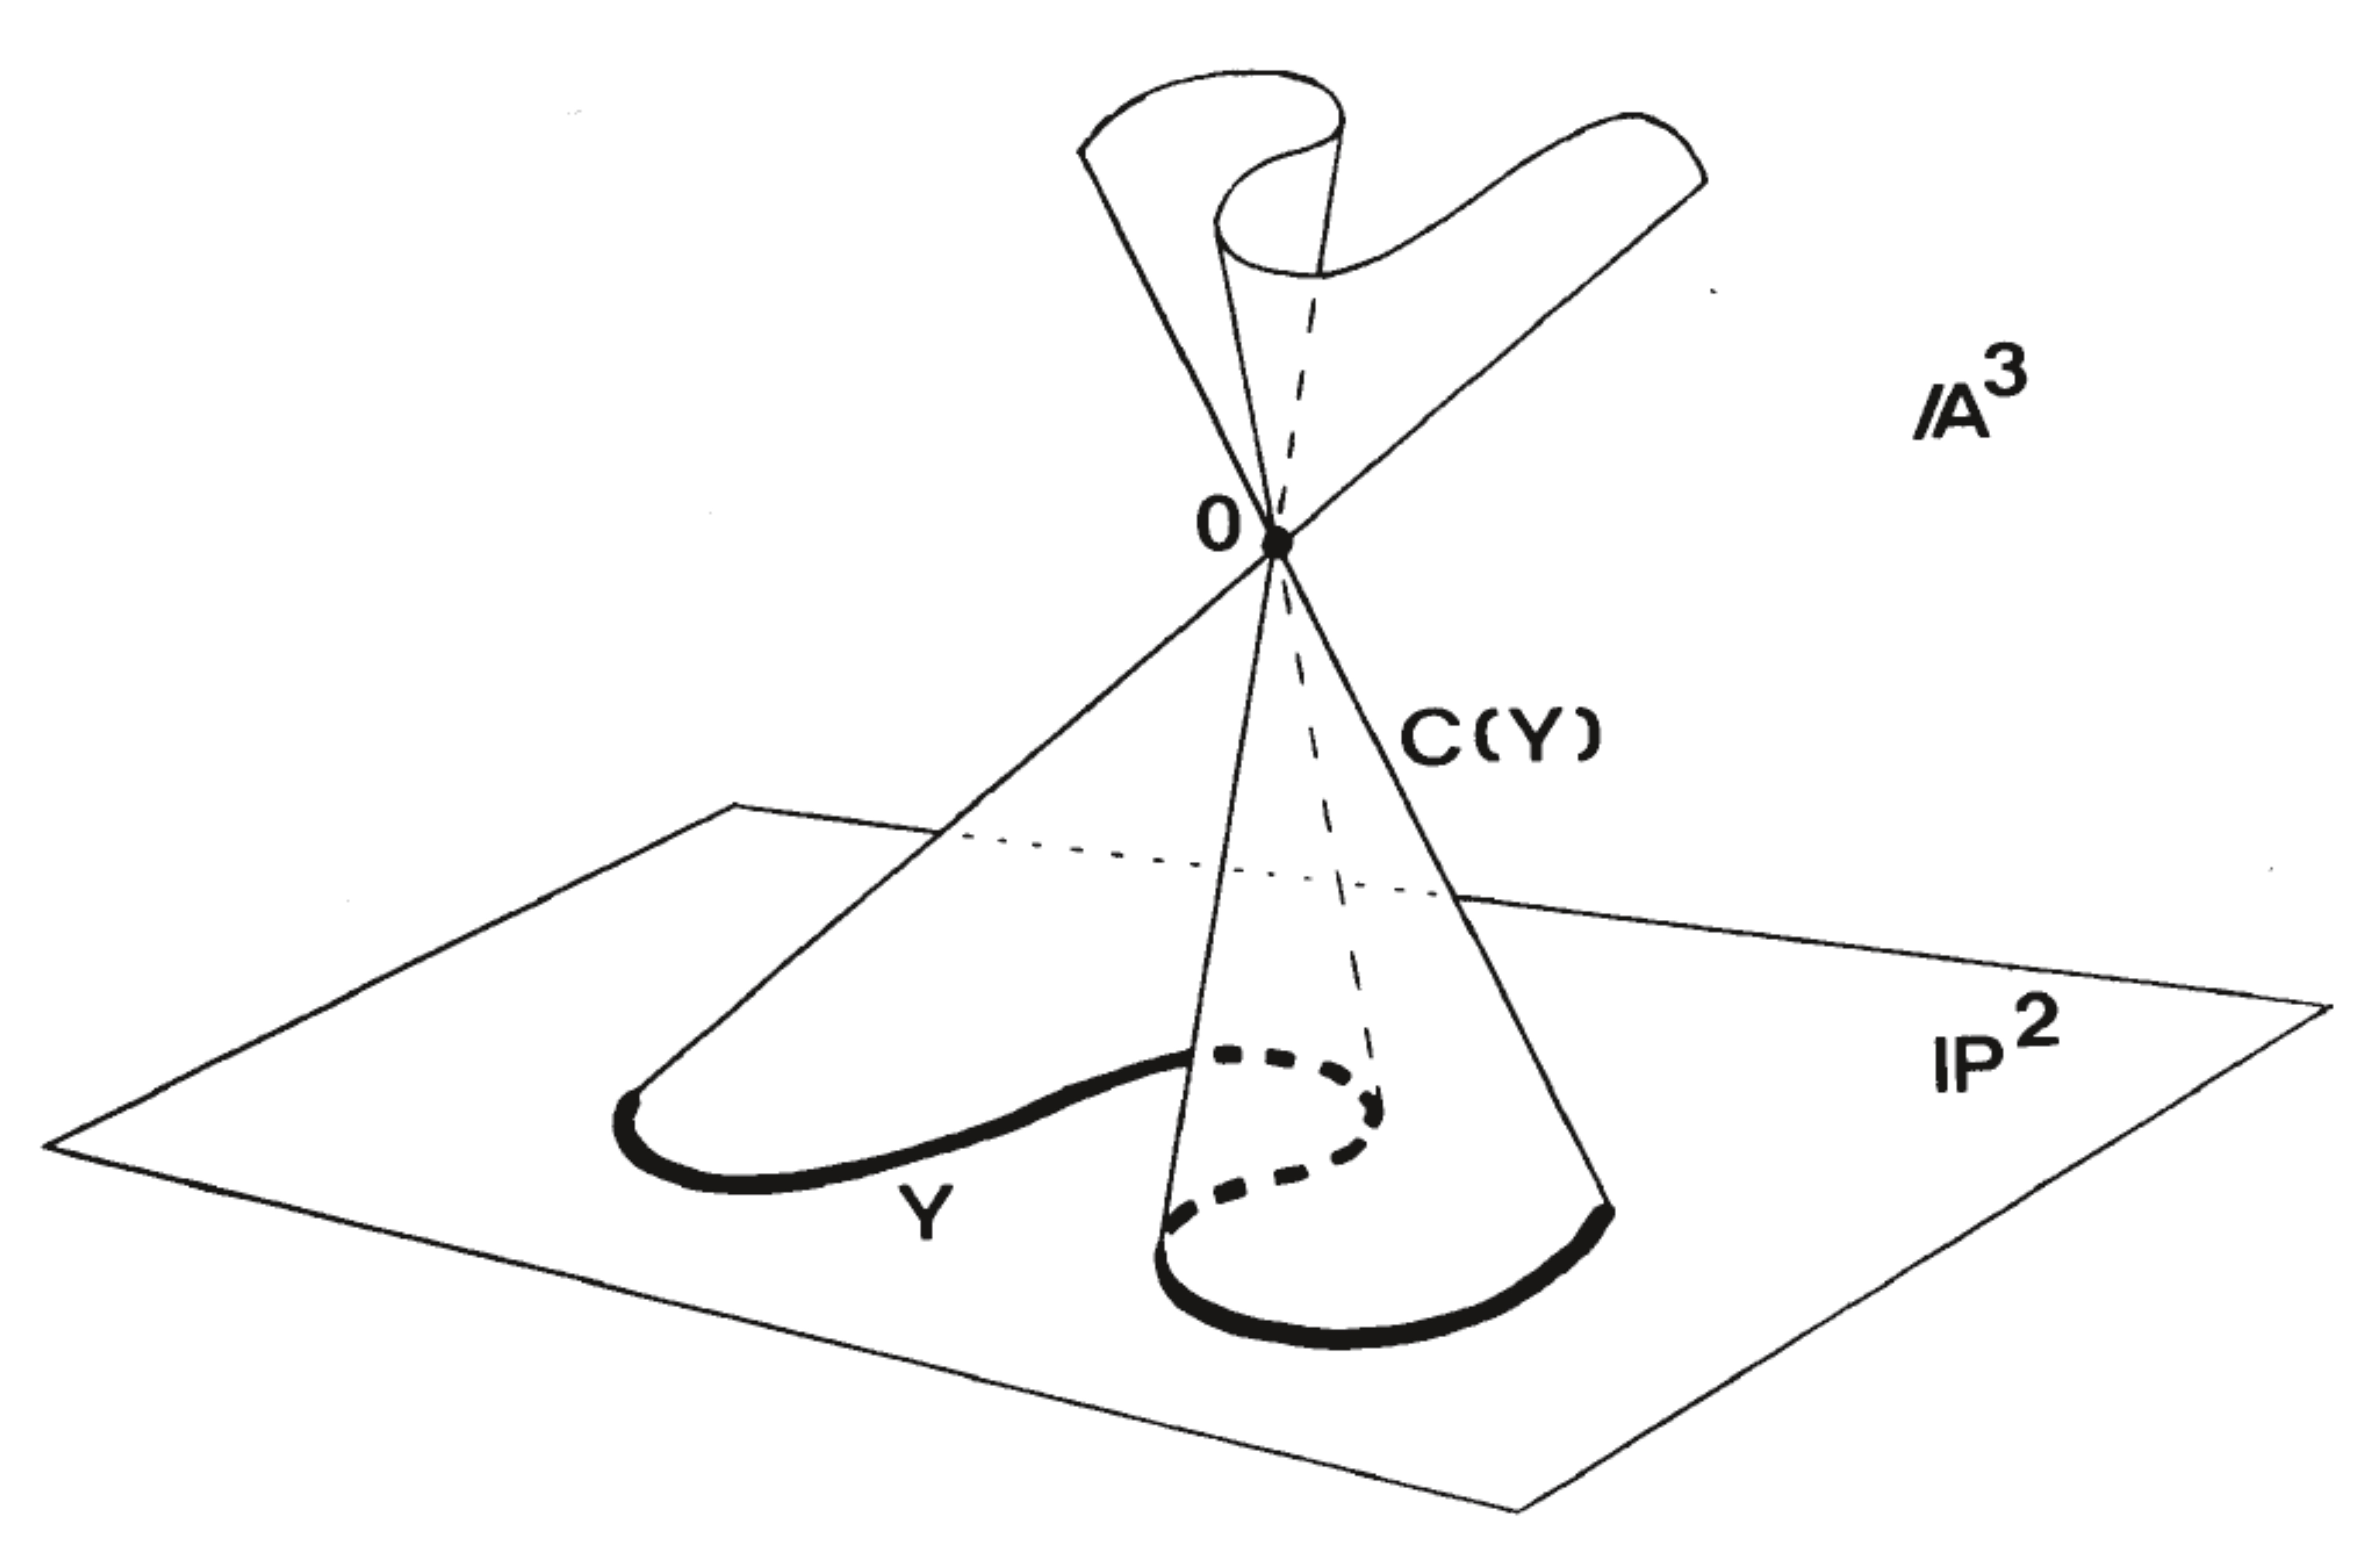
\includegraphics[width=0.5\columnwidth]{Figure1}\\
	Figure 1. $\mb P^2$에서의 곡선 상에서의 뿔
	\end{center}
	%
	\begin{enumerate}[label=,itemindent=0mm]
	\item Sol) (a) $I(Y)$가 동차 원소들에 의해 생성되므로 자명하다.\\
	(b) $C(Y)$가 기약 iff $I(Y)$가 소 아이디얼 iff $Y$가 기약.\\
	(c) $Y$가 기약일 경우 (Ex. 2.6)에 의해 $\dim Y+1=\dim S(Y)=(n+1)-\mrm{height}\:I(Y)=\dim A(C(Y))=\dim C(Y)$이다.\\
	$Y$가 기약이 아닌 경우 $Y$의 기약 성분이 $Y_1,\ldots,Y_n$이라 하자.
	$C(Y_1),\ldots,C(Y_n)$은 유한 개이고 (b)에 의해 기약이며 아핀 뿔의 정의에 의해 서로를 포함하지 않는다.
	따라서 Proposition 1.5의 유일성에 의해 이들은 $C(Y)$의 기약 성분들이다.
	각각의 $Y_i$가 기약이므로 $\dim Y_i+1=\dim C(Y_i)\:(1\le i\le n)$이 성립한다.
	$\dim Y=\max_i\dim Y_i,\dim C(Y)=\max_i\dim C(Y_i)$이므로 $\dim Y+1=\dim C(Y)$이다.\\
	\end{enumerate}
	%
	\begin{enumerate}[label=\tb{2.\arabic*.},itemindent=0mm,itemsep=4mm]
		\setcounter{enumi}{10}
		\item \tb{$\Pn$에서의 선형 대수다양체}. 1차다항식에 의해 정의된 초곡면은 \tb{초평면(hyperplane)}이라 불린다.
		\begin{enumerate}[label=(\alph*)]
			\item $\Pn$에서의 대수다양체 $Y$에 대한 다음 두 조건이 동치임을 보여라:
			\begin{enumerate}[label=(\roman*)]
				\item $I(Y)$는 1차다항식들에 의해 생성될 수 있다.
				\item $Y$는 초평면들의 교집합으로 표현될 수 있다.
			\end{enumerate}
			이 경우 우리는 $Y$가 $\Pn$에서의 \tb{선형 대수다양체(linear variety)}라 한다.
			\item 만약 $Y$가 $\Pn$에서의 $r$차원 선형 대수다양체이면
			$I(Y)$가 최소 $n-r$개의 1차다항식에 의해 생성됨을 보여라.
			\item $Y,Z$가 $\Pn$에서의 선형 대수다양체이며 $\dim Y=r,\dim Z=s$라 하자.
			만약 $r+s-n\ge 0$이면 $Y\cap Z\ne\es$이다.
			이에 더해 만약 $Y\cap Z\ne\es$이면 $Y\cap Z$는 차원 $r+s-n$ 이상의 선형 대수다양체이다.
			($\mb A^{n+1}$을 $k$ 상에서의 벡터 공간으로 간주하고 그 부분공간에서 작업하라.)
		\end{enumerate}
		\sol (a) 대수적 집합들의 교집합의 아이디얼은 아이디얼들의 합집합이다.\\
		(b) 사영공간을 아핀 열린집합 $U_i$들에 의해 덮고 (Ex. 1.9, 1.10b)를 적용하면 따라온다.\\
		(c) $\mb A^{n+1}$에서의 아핀 뿔을 고려하자. $Y$와 $Z$의 아핀 뿔은 벡터 공간으로 간주된 $\mb A^{n+1}$의
		$r+1$차원과 $s+1$차원 선형 부분공간이다. 따라서 그 교집합인 $Y\cap Z$의 아핀 뿔은
		$\mb A^{n+1}$의 $(r+1)+(s+1)-(n+1)=r+s-n+1$차원 이상의 선형 부분공간이다.
		그러므로 $Y\cap Z$는 $r+s-n$차원 이상의 선형 대수다양체이다.
		\item \tb{$d$차 매장}. 주어진 $n,d>0$에 대하여 $M_0,M_1,\ldots,M_N$이
		$n+1$개 변수 $x_0,\ldots,x_n$에 대한 모든 $d$차 단항식들이라 하자. 여기에서 $N=\binom{n+d}{n}-1$이다.
		함수 $\rho_d:\Pn\ra\mb P^N$을 점 $P=(a_0,\ldots,a_n)$을 단항식 $M_j$들에 $a_i$들을 대입하여 얻어진
		점 $\rho_d(P)=(M_0(a),\ldots,M_N(a))$로 대응시키는 함수로 정의하자.
		이는 $\Pn$에서 $\mb P^N$으로의 \tb{$d$차 매장($d$-uple embedding)}이라 불린다.
		예를 들어 만약 $n=1,d=2$이면 $N=2$이고 $\mb P^1$의 $\mb P^2$로의 $2$차 매장의 상 $Y$는 원뿔곡선이다.
		\begin{enumerate}[label=(\alph*)]
			\item $\ta:k[y_0,\ldots,y_N]\ra k[x_0,\ldots,x_n]$이
			$y_i$를 $M_i$로 대응시키는 것으로 정의된 준동형사상이며 $\mf a$가 $\ta$의 핵이라 하자.
			그 경우 $\mf a$는 동차 소 아이디얼이며 따라서 $Z(\mf a)$는 $\mb P^N$에서의 사영 대수다양체이다.
			\item $\rho_d$의 상이 정확히 $Z(\mf a)$임을 보여라. (한쪽 포함 관계는 간단하다. 반대쪽은 계산이 필요하다.)
			\item 이제 $\rho_d$가 $\Pn$에서 사영 대수다양체 $Z(\mf a)$로의 위상동형사상임을 보여라.
			\item $\mb P^3$에서의 비틀린 3차곡선(Ex. 2.9)이 적절한 좌표 선택 하에서
			$\mb P^1$의 $\mb P^3$으로의 3차 매장과 동일함을 보여라.
		\end{enumerate}
		\sol (a) $k[y_0,\ldots,y_N]$에 속한 다항식 $f$가 $\ta$에 의해 0으로 대응된다면
		$\ta$가 동차성을 보존하므로 $f$의 동차 성분들도 0의 동차 성분들, 즉 0으로 대응된다. 그러므로 $\mf a$는 동차 아이디얼이다.
		다음으로 $fg\in\mf a$이면 $\ta(fg)=\ta(f)\ta(g)=0$이며 따라서 $f$ 또는 $g$가 $\mf a$가 속한다.
		그러므로 $\mf a$는 소 아이디얼이며 $Z(\mf a)$는 사영 대수다양체이다.\\
		(b) $f\in\mf a=\ker\ta$ iff $f(M_0,\ldots,M_N)=0$이므로 $\Im\rho_d\bseq Z(\mf a)$임은 자명하다.\\
		$f\in I(\Im\rho_d)$라 하자. 그 경우 모든 $x\in\Im\rho_d$에 대하여 $f(x)=0$이며
		따라서 임의의 $(a_0,\ldots,a_n\in\Pn)$에 대하여 $f(M_0(a),\ldots,M_N(a))=0$이다.
		즉 $f(M_0,\ldots,M_N)$은 $n+1$변수 다항식이며 항등적으로 0이다.
		$k$가 무한체이므로 이는 $f(M_0,\ldots,M_N)=0$임을 함의한다.
		그러므로 $\mf a\pseq I(\Im\rho_d)$이며 $Z(\mf a)\bseq Z(I(\Im\rho_d))$이다.
		이제 $\Im\rho_d$가 $\mb P^N$에서의 Zariski 닫힌집합이며 따라서 $Z(I(\Im\rho_d))=\Im\rho_d$임을 보여야 한다.
		$\sum t_i=d$인 경우 $j(t_1,\ldots,t_n)$가 $M_{j(t_1,\ldots,t_n)}(a)=a_1^{t_1}\cdots a_n^{t_n}$을 만족시키는 수라 하자.
		또한 각각의 $i$에 대하여 $j_0(i)$를 $M_{j_0(i)}(a)=a_i^d$를 만족시키는 수로 정의하고
		$j_1(i,j)$를 $M_{j_1(i,j)}(a)=a_i^{d-1}a_j$를 만족시키는 수로 정의하자.\\
		$\Im\rho_d$가 다항식 $y_{j(t_0,\ldots,t_n)}y_{j(s_0,\ldots,s_n)}-y_{j(t'_0,\ldots,t'_n)}y_{j(s'_0,\ldots,s'_n)}
		\:(t_i+s_i=t'_i+s'_i)$들의 영점집합임을 보이자. $\Im\rho_d$의 점들이 이러한 다항식들을 만족시킴은 명백하다.
		역으로 이러한 영점집합에 속하는 임의의 점 $y_i=b_i$를 선택하자. 그 경우 모든 좌표 $b_{j_0(i)}$들이 동시에 0일 수 없다;
		이 경우 위 다항방정식들에 의해 $(b_0,\ldots,b_N)=(0,\ldots,0)$이 되어 모순이다.
		따라서 어떠한 좌표 $b_{j_0(i)}$가 0이 아니다. w.l.o.g. $b_{j_0(0)}=1$이라 하자.
		$a_0=1$로, $a_i=b_{j_1(0,i)}$로 정의하자. 그 경우 위 다항방정식들을 반복적용하면 $b_{j(t_0,\ldots,t_n)}
		=a_1^{t_1}a_2^{t_2}\cdots a_n^{t_n}=M_{j(t_0,\ldots,t_n)}(a)$를 얻는다. 따라서 이 점은 $\Im\rho_d$에 속한다.\\
		(c) 모든 좌표함수가 $d$차 동차 다항함수이므로 $\rho_d$는 Zariski 위상 하에서 연속 함수이다. (cf. Lemma 3.6)
		$\rho_d$의 역함수는 $y_{j_0(i)}\ne 0$인 조밀 열린집합 상에서 좌표 표현
		$(y_{j_1(i,0)},\ldots,y_{j_1(i,i-1)},y_{j_1(i,i+1)},\ldots,y_{j_1(l,n)})$으로 주어지므로 연속하다.
		이러한 조밀 열린 부분집합들은 $\Im\rho_d$의 덮개를 형성한다. 그러므로 이는 $\Im\rho_d$ 전체 상에서 연속하다.
		(역함수를 명시적으로 구축할 수 있으므로 $\rho_d$는 단사이다.) 따라서 $\rho_d$는 위상동형사상이다.\\
		(d) $\mb P^1$의 3차 매장은 $(x,y)\mt(x^3,x^2y,xy^2,y^3)$이다. 이는 (Ex 2.9)에서 얻은 비틀림 3차곡선의 매개변수 표현이다.
		\item $Y$가 $\mb P^2$의 $\mb P^5$로의 2차 매장의 상이라 하자. 이는 \tb{Veronese 곡면(Veronese surface)}이다.
		만약 $Z\bseq Y$가 닫힌 곡선이면(\tb{곡선(curve)}은 1차원 대수다양체이다)
		$V\cap Y=Z$를 만족시키는 초곡면 $V\bseq\mb P^5$가 존재함을 보여라.\\
		\sol $\mb P^2$의 2차 매장은 $(x,y,z)\mt(x^2,y^2,z^2,xy,yz,zx)$이다.
		2차 매장이 그 상으로의 대수다양체 동형사상이므로 (cf. (Ex. 2.13c), Section I.3)
		$Z$는 $\mb P^2$에서의 곡선으로 간주될 수 있으며 따라서 이는 $x,y,z$에 대한 동차다항식 $f$에 의해 정의된다.
		$f^2$는 짝수차 동차다항식이며 따라서 $x^2,y^2,z^2,xy,yz,zx$에 대한 다항식으로 표현 가능하다.
		(이러한 표현 방식은 유일하지 않다; 특정한 한 가지를 선택하자.
		예를 들어 각각의 항에서 $x,y,z$를 가능한 한 많이 $x^2,y^2,z^2$로 묶으면 $1$ 또는 $xy,yz,zx$ 중 정확히 하나가 남는다.)
		여기에서 변수를 $y_0,\ldots,y_5$로 대체한 다항식을 $g$라 하자.
		그 경우 $Y$의 모든 점은 $(x^2,y^2,z^2,xy,yz,zx)$로 표현되므로 $\mb P^5$에서의 $Z(g)\cap Y$는
		$\mb P^2$에서의 $Z(f^2)=Z(f)$에 대응된다. i.e. $Z(g)\cap Y=Z$가 성립한다.
		$Z$가 기약이므로 $Z(g)$의 어떠한 기약 성분 $Z(g_1)$이 존재하여 $Z(g_1)\ps Z$를 만족시킨다. 
		(여기에서 $g_1$은 $g$의 어떠한 기약 인수이다.) $Z(g_1)$이 요구된 초곡면 $V$이다.
		\item \tb{Segre 매장}. $\psi:\mb P^r\times\mb P^s\ra\mb P^N$이 순서 쌍 $(a_0,\ldots,a_r)\times(b_0,\ldots,b_s)$를
		사전 순서인 $(\ldots,a_ib_j,\ldots)$로 대응시키는 것으로 정의된 함수라 하자. 여기에서 $N=rs+r+s$이다.
		$\psi$가 잘 정의되었으며 단사임을 기억해 두라. 이는 \tb{Segre 매장(Segre embedding)}이라 불린다.
		$\psi$의 상이 $\mb P^N$의 \tb{부분대수다양체(subvariety)}임을 보여라.
		[Hint: $\mb P^N$의 동차 좌표가 $\sx{z_{ij}}{i=0,\ldots,r,j=0,\ldots,s}$라 하고
		$\mf a$가 $z_{ij}$를 $x_iy_j$로 대응시키는 준동형사상 $k[\{z_{ij}\}]\ra k[x_0,\ldots,x_r,y_0,\ldots,y_s]$의 핵이라 하자.
		그 후 $\Im\psi=Z(\mf a)$임을 보여라]\\
		\sol $f\in\mf a$ iff $f(x_0y_0,\ldots,x_ry_s)=0$이므로 (Ex. 2.12b)에서와 같은 논의에 의해 $\Im\psi=Z(\mf a)$이다.
		($\mf a$는 $z_{ij}z_{kl}-z_{kj}z_{il}$들에 의해 생성된다.)
		\item \tb{$\mb P^3$에서의 2차곡면} (Fig. 2). 방정식 $xy-zw=0$에 의해 정의된 $\mb P^3$에서의 곡면 $Q$를 고려하자.
		(\tb{곡면(surface)}은 2차원 대수다양체이다.)
		\begin{enumerate}[label=(\alph*)]
			\item $Q$가 적절한 좌표 선택 하에서 $\mb P^1\times\mb P^1$의 $\mb P^3$으로의 Segre 매장과 동일함을 보여라.
			\item $Q$가 $t\in\mb P^1$에 의해 매개화된 다음을 만족시키는 직선들의 두 개의 족 $\{L_t\},\{M_t\}$를 포함함을 보여라:
			(\tb{직선(line)}은 1차원 선형 대수다양체이다.)
			만약 $L_t\ne L_u$이면 $L_t\cap L_u=\es$, 만약 $M_t\ne M_u$이면 $M_t\cap M_u=\es$,
			모든 $t,u$에 대하여 $L_t\cap M_u=$ 한 점.
			\item $Q$가 이러한 직선들 이외에도 다른 곡선들을 포함함을 보이고 $Q$ 상에서의 Zariski 위상이
			$\mb P^1\times\mb P^1$ 상에서의 곱위상(여기에서 각각의 $\mb P^1$은 Zariski 위상을 가진다.)과
			$\psi$를 통해 위상동형이 아님을 보여라.
		\end{enumerate}
		\end{enumerate}
		%Figure 2
		\begin{center}
			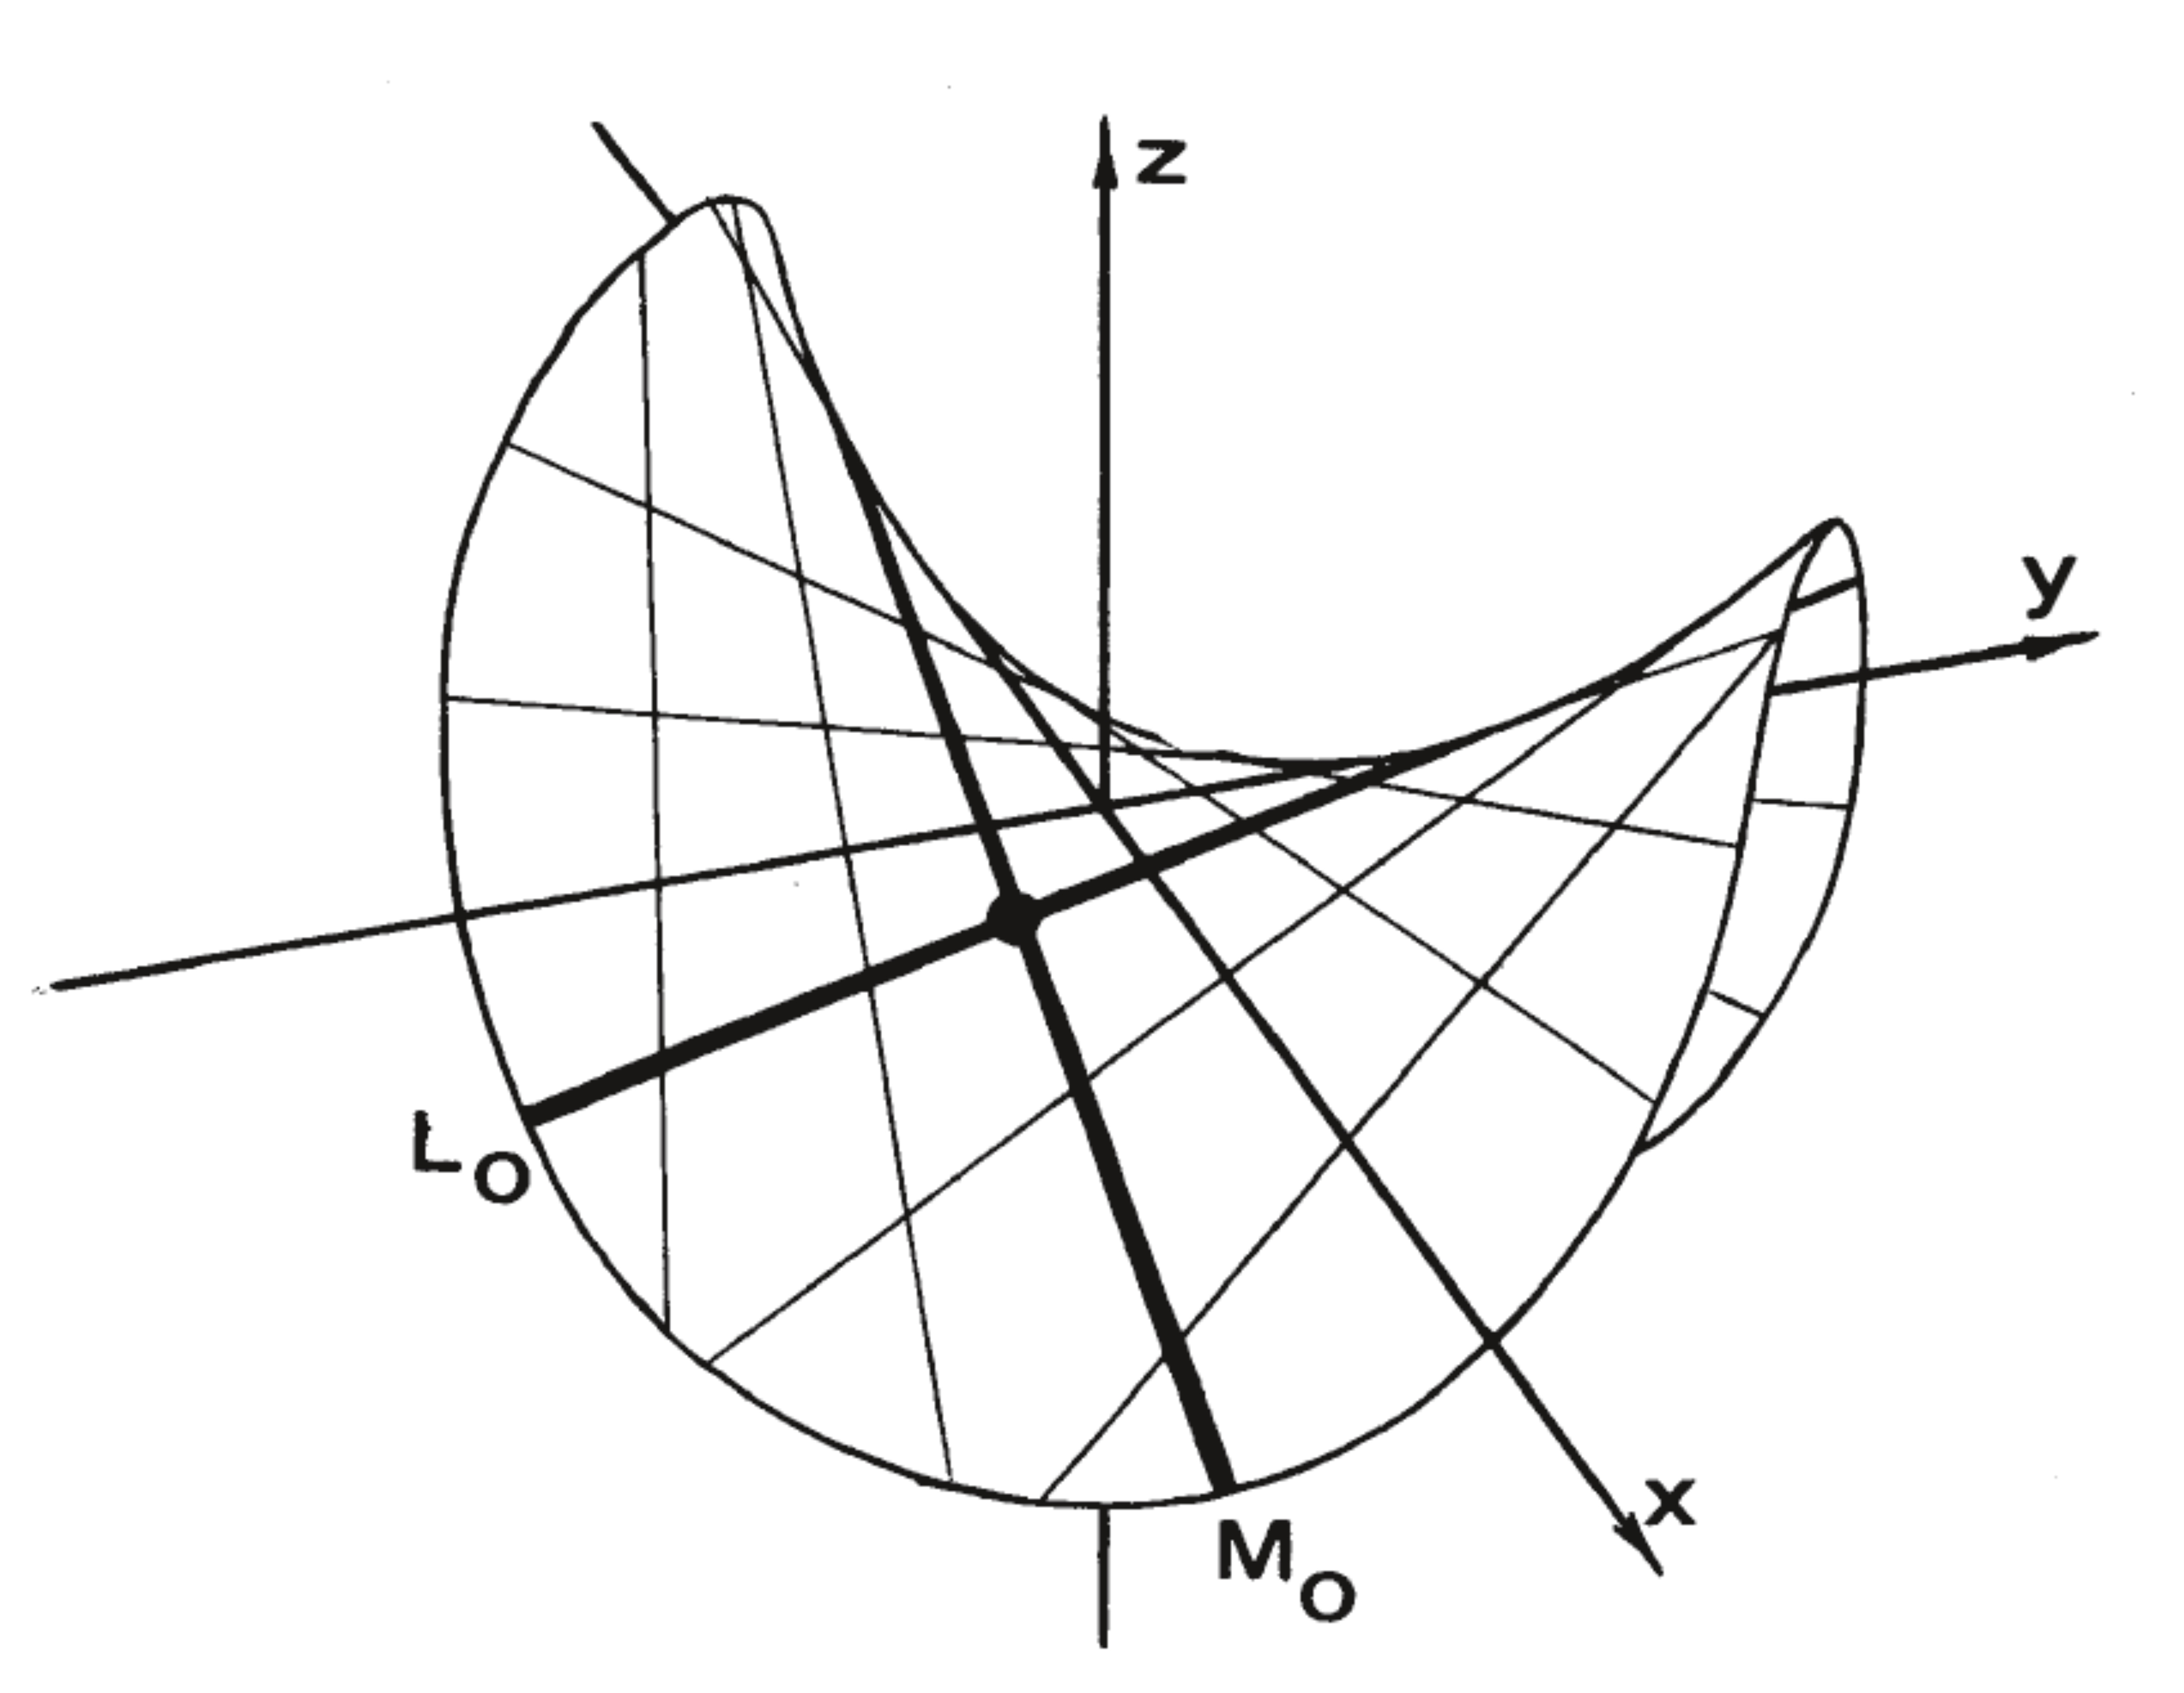
\includegraphics[width=0.5\columnwidth]{Figure2}\\
			Figure 2. $\mb P^3$에서의 2차곡면
		\end{center}
		%
		\begin{enumerate}[label=,itemindent=0mm]
		\item Sol) (a) $\mb P^1\times\mb P^1$의 Segre 매장은 $(x_0,x_1,y_0,y_1)\mt(x_0y_0,x_0y_1,x_1y_0,x_1y_1)=(w,x,y,z)$이다.
		(Ex. 2.14)에서 보였듯이 그 상의 아이디얼은 $z_{ij}z_{kl}-z_{kj}z_{il}$들에 의해 생성되며
		이들 중 자명하지 않은 원소는 $xy-zw$뿐이다. 따라서 $(xy-zw)$는 제시된 Segre 매장이다.\\
		(b) $L_t:Z(x-tz,y-tw)$ 및 $M_t:Z(x-tw,y-tz)$들이 요구된 직선이다.\\
		(c) $Q$에서는 $Z(xy-zw,x-y)$ 등 직선이 아닌 곡선도 존재한다. 그러나 Zariski 위상의 곱위상 하에서는
		모든 닫힌집합이 두 $\mb P^1$ 중 하나에 평행한 직선들의 유한 합집합이다.
		이러한 집합은 $\psi$에 의해 $Q$에서의 직선들의 유한 합집합으로 대응된다. 그러므로 이들은 위상동형이 아니다.\\
		\end{enumerate}
		\begin{enumerate}[label=\tb{2.\arabic*.},itemindent=0mm,itemsep=4mm]
		\setcounter{enumi}{15}
		\item \begin{enumerate}[label=(\alph*)]
			\item 두 대수다양체의 교집합이 대수다양체여야 할 필요는 없다.
			예를 들어 $Q_1$과 $Q_2$가 각각 방정식 $x^2-yw=0$과 $xy-zw=0$에 의해 주어진 $\mb P^3$에서의 2차곡면이라 하자.
			$Q_1\cap Q_2$가 비틀린 3차곡선과 직선의 합집합임을 보여라.
			\item 두 대수다양체의 교집합이 대수다양체이더라도 교집합의 아이디얼은 아이디얼들의 합이 아닐 수 있다.
			예를 들어 $C$가 방정식 $x^2-yz=0$에 의해 주어진 $\mb P^2$에서의 2차곡선이라 하자.
			$L$이 $y=0$에 의해 주어진 직선이라 하자. $C\cap L$이 한 점 $P$로 구성되어 있지만 $I(C)+I(L)\ne I(P)$임을 보여라.
		\end{enumerate}
		\sol (a) 아핀 열린집합 $w=1$에서 이는 $x^2-y=0,xy-z=0$이므로 이는 $(w,x,y,z)=(1,x,x^2,x^3)$인 비틀린 3차곡선이다.
		$Q_1\cap Q_2$가 닫힌집합이므로 이는 아핀 비틀린 3차곡선의 사영 폐포인 사영 비틀린 3차곡선을 포함한다.
		닫힌집합 $w=0$에서 이는 $x^2=xy=0$이므로 직선 $x=w=0$이다.\\
		(b) $C\cap L$은 한 점 $P=(0,0,z)$으로 구성된다. $x$는 $I(P)=(x,y)$에 속하지만 $I(C)+I(L)=(x^2-yz,y)$에 속하지 않는다.
		\item \tb{완비 교집합}. $\Pn$에서의 $r$차원 대수다양체 $Y$가 \tb{(강)완비 교집합((strict) complete intersection)}이라는
		것의 정의는 $I(Y)$가 $n-r$개 원소에 의해 생성될 수 있는 것이다.
		$Y$가 \tb{집합론적 완비 교집합(set-theoretic complete intersection)}이라는 것의 정의는
		$Y$가 $n-r$개 초곡면의 교집합으로 표현 가능한 것이다.
		\begin{enumerate}[label=(\alph*)]
			\item $Y$가 $\Pn$에서의 대수다양체이며 $Y=Z(\mf a)$라 하자. 또한 $\mf a$가 $q$개 원소에 의해 생성될 수 있다 하자.
			그 경우 $\dim Y\ge n-q$임을 보여라.
			\item 강완비 교집합이 집합론적 완비 교집합임을 보여라.
		\end{enumerate}
		\begin{enumerate}[label=*(\alph*)]
			\setcounter{enumii}{2}
			\item (b)의 역은 거짓이다. 예를 들어 $Y$가 $\mb P^3$에서의 비틀린 3차곡선이라 하자. (Ex. 2.9)
			$I(Y)$가 두 원소에 의해 생성될 수 없음을 보여라.
			반면에 $Y=H_1\cap H_2$를 만족시키는 각각 2차와 3차인 초곡면 $H_1,H_2$를 찾아라.
		\end{enumerate}
		\begin{enumerate}[label=**(\alph*)]
			\setcounter{enumii}{3}
			\item $\mb P^3$에서의 모든 닫힌 기약 곡선이 두 곡면의 집합론적 교집합인지는 아직 해결되지 않은 문제이다.
			해설에 대해서는 Hartshorne [1]과 Hartshorne [5, III, \S 5]를 참조하라.
		\end{enumerate}
		\sol (a) 사영공간을 아핀 열린집합 $U_i$들에 의해 덮고 (Ex. 1.9, 1.10b)를 적용하면 따라온다.\\
		(b) $Y$가 강완비 교집합이면 $I(Y)$의 $n-r$개 생성자들은 각각 초곡면을 정의하며
		$Y$는 이러한 초곡면들의 교집합이므로 집합론적 완비 교집합이다.\\
		(c) $Y=\sx{(w,x,y,z)=(t^3,t^2s,ts^2,s^3)}{t,s\in k}$이다.
		$Y$ 상에서 소멸하는 1차 동차다항식은 존재하지 않으며 $Y$ 상에서 소멸하는 2차 동차다항식은 $x^2-yw,y^2-zx,xy-zw$이다.
		이들은 서로를 생성하지 못하므로 $Y$의 아이디얼의 생성집합에는 이 세 원소가 반드시 포함되어야 한다.
		따라서 $Y$는 강완비 교집합이 아니다. 반면에 아핀 비틀린 3차곡선 $Y_0=Z(x^2-yw)\cap Z(x^3-zw^2)$(아핀 공간의 영점집합)이므로
		그 사영 폐포를 취하면 $Y=Z(x^2-yw)\cap Z(x^3-zw^2)$(사영 공간의 영점집합)이며 $Y$는 집합론적 완비 교집합이다.
	\end{enumerate}
	
	
	\subsection*{Section I.3}
	
	\begin{enumerate}[label=\tb{3.\arabic*.},itemindent=0mm,itemsep=4mm]
		\item \begin{enumerate}[label=(\alph*)]
			\item $\mb A^2$에서의 임의의 원뿔곡선이 $\mb A^1$ 또는 $\mb A^1-\{0\}$과 동형임을 보여라. (cf. Ex. 1.1)
			\item $\mb A^1$이 자신의 임의의 열린 진부분집합과 동형이 \ti{아님}을 보여라.
			(이 결과는 아래의 Ex. 6.7)에서 일반화된다.
			\item $\mb P^2$에서의 임의의 원뿔곡선은 $\mb P^1$과 동형이다.
			\item 우리는 나중에 (Ex. 4.8) 임의의 두 곡선이 위상동형임을 보일 것이다.
			그러나 $\mb A^2$는 심지어 $\mb P^2$와도 위상동형이 아님을 보여라.
			\item 만약 아핀 대수다양체가 사영 대수다양체와 동형이면 이는 한 점으로만 구성됨을 보여라.
		\end{enumerate}
		%
		\sol (a) Ex. 1.1에서 임의의 원뿔곡선 $Y$의 아핀 좌표환이 $k[x]$ 또는 $k[x,x^{-1}]$임을 보였다.
		이는 각각 $\mb A^1$과 $\mb A^1-\{0\}$의 아핀 좌표환이며 따라서 $Y$는 이들 중 하나와 동형이다.\\
		(b) $\mb A^1$의 열린 진부분집합은 $\mb A^1$에서 유한 개 점을 제외한 것이다.
		이는 평행이동에 의해 $\mb A^1-\{0,1,\ldots,n\}$과 동형이다. 이는 다시 (아핀 좌표계 $x,x_0,x_1,\ldots,x_n$을 가지는)
		$\mb A^{n+2}$에서의 초곡면 $xx_0=(x-1)x_1=(x-2)x_2=\cdots=(x-n)x_n=1$과 첫째 좌표 $x$로의 사영을 통해 동형이다.
		그 아핀 좌표환은 $k[x,x_0,x_1,\ldots,x_n]/(xx_0-1,(x-1)x_1-1,\ldots,(x-n)x_n-1)
		\cong k[x,x^{-1},(x-1)^{-1},\ldots,(x-n)^{-1}]$이다.
		그러나 이는 $\mb A^1$의 아핀 좌표환 $k[x]$와 동형이 아니므로 $\mb A^1$과 $\mb A^1-\{0,1,\ldots,n\}$은 동형이 아니다.\\
		(c) 사영평면의 원뿔곡선을 표현하는 동차다항식을 $z=1$을 대입하여 탈동차화하고 이를 Ex. 1.1에서와 같은 방식으로 변형한 후
		다시 동차화하면 다음을 얻는다: $f=x^2+axz+byz+cz^2\:(b\ne 0)$ 또는 $f=xy-z^2$.
		전자는 $ax+by+cz=-y'$으로 정의하면 $x^2-y'z$이므로 후자와 동일한 형태이다.
		따라서 사영평면의 모든 이차곡선은 $xz-y^2=0$과 동형이다.
		이는 2차 매장 $\mb P^1\ra\mb P^2$(Ex. 2.12)의 상이므로 $\mb P^1$과 동형이다. (cf. Ex. 3.4)\\
		(d) $\mb P^2$에서의 임의의 두 직선(1차원 기약 닫힌집합)은 교차하나 $\mb A^2$에서는 그렇지 않다.
		그러므로 이들은 위상동형이 아니다.\\
		(e) 아핀 대수다양체 $X$와 사영 대수다양체 $Y$가 동형이면 정칙함수환이 같아야 한다.
		$k\cong\mc O(Y)\cong\mc O(X)\cong A(X)$이므로 $X$는 한 점이다.
		%
		\item 기반 함수가 위상 공간 간의 위상동형인사상인 사상은 동형사상일 필요가 없다.
		\begin{enumerate}[label=(\alph*)]
			\item 예를 들어 $\ph:\mb A^1\ra\mb A^2$가 $t\mt(t^2,t^3)$으로 정의되었다 하자.
			$\ph$가 $\mb A^1$에서 곡선 $y^2=x^3$으로의 전단사 쌍연속 사상을 정의하지만 동형사상은 아님을 보여라.
			\item 다른 예를 위해, 기반체 $k$의 표수가 $p>0$이라 하고 함수 $\ph:\mb A^1\ra\mb A^1$을 $t\mt t^p$로 정의하자.
			$\ph$가 전단사 쌍연속이지만 동형사상은 아님을 보여라. 이는 \tb{Frobenius 사상(Frobenius morphism)}이라 불린다.
		\end{enumerate}
		%
		\sol (a) 각각의 좌표함수가 다항함수이므로 $\ph$는 대수다양체 사상이며 따라서 연속하다. 전단사임은 자명하다.
		$\ph$는 닫힌집합인 $\mb A^1$, 한 점, 공집합을 각각 $y^2=x^3$, 한 점, 공집합으로 대응시키므로 닫힌 함수이다.
		전단사 연속 닫힌 함수이므로 $\ph$는 쌍연속이며 위상동형사상이다.
		그러나 $\ph^{-1}$은 원점 근방에서 유리함수로 표현 불가하므로 대수다양체 사상이 아니며
		따라서 $\ph$가 대수다양체 동형사상이 아니다.\\
		(b) $k$가 대수적으로 닫힌 체이므로 모든 원소는 $p$제곱근을 가지며 따라서 $\ph$가 전사이다.
		$x^p-y^p=0$이면 $(x-y)^p=0$이고 $x-y=0$이므로 $\ph$가 단사이다.
		(a)에서와 같은 논의에 의해 $\ph$는 위상동형사상이지만 역함수가 유리함수로 표현 불가하므로 대수다양체 동형사상이 아니다.
		%
		\item \begin{enumerate}[label=(\alph*)]
			\item $\ph:X\ra Y$가 사상이라 하자. 그 경우 각각의 $P\in X$에 대하여
			$\ph$는 국소환의 준동형사상 $\ph_P^*:\mc O_{\ph(P),Y}\ra\mc O_{P,X}$를 유도한다.
			\item 사상 $\ph$가 동형사상일 필요충분조건은 $\ph$가 위상동형사상이며
			모든 $P\in X$에 대하여 국소환 상에 유도된 함수 $\ph_P^*$가 동형사상인 것임을 보여라.
			\item 만약 $\ph(X)$가 $Y$에서 조밀하면 모든 $P\in X$에 대하여 함수 $\ph_P^*$가 \ti{단사}임을 보여라.
		\end{enumerate}
		%
		\sol (a) $\ph_P^*:\mc O_{\ph(P),Y}\ra\mc O_{P,X}$를 $\bk{U,f}\mt\bk{\ph^{-1}(U),f\circ\ph}$로 정의하자.
		이것이 환 연산을 보존함은 자명하다.\\
		(b) ($\Ra$) $\ph$가 동형사상이면 Lemma 3.6에 의해 $\ph_P^*$들과 ${\ph^{-1}}_{\ph(P)}^*$들이 모두 환 준동형사상이다.
		이들은 서로의 역이므로 $\ph_P$가 환 동형사상이다.\\
		($\La$) $(\ph_P^*)^{-1}={\ph^{-1}}_{\ph(P)}^*$가 잘 정의됨은 $\ph^{-1}$이 대수다양체 사상임을 함의한다.\\
		(c) $\ph^*:f\mt f\circ\ph$로 정의하자. $\ph^*(f)=0$이라 가정하자. 그 경우 어떠한 근방 $\ph(U)\bs Y$ 상에서 $f=0$이다.
		만약 $f\ne 0$이면 $\ph(X)\bseq Z(f)\bsneq Y$이며 $\ph(X)$의 조밀성에 모순이다.
		%
		\item $\Pn$의 $d$차 매장(Ex. 2.12)가 그 상으로의 동형사상임을 보여라.\\
		%
		\sol $d$차 매장 $\rho_d$의 모든 좌표가 동차 다항함수이므로 $\rho_d$는 대수다양체 사상이다.
		각각의 $i$에 대하여 $j_0(i)$를 $M_{j_0(i)}(a)=a_i^d$를 만족시키는 수로 정의하고
		$j_1(i,j)$를 $M_{j_1(i,j)}(a)=a_i^{d-1}a_j$를 만족시키는 수로 정의하자.
		$\rho_d$의 역함수는 $y_{j_0(i)}\ne 0$인 조밀 열린집합 상에서 좌표 표현\\
		$(y_{j_1(i,0)},\ldots,y_{j_1(i,i-1)},y_{j_1(i,i+1)},\ldots,y_{j_1(l,n)})$으로 주어진다.
		이러한 조밀 열린 부분집합들은 $\Im\rho_d$의 덮개를 형성한다. 따라서 $\rho_d$는 대수다양체 동형사상이다.
		%
		\item 언어를 남용하여 대수다양체가 `아핀'이라는 것을 아핀 대수다양체와 동형인 것이라 하겠다.
		만약 $H\bseq\Pn$이 임의의 초곡면이면 $\Pn-H$가 아핀임을 보여라. [Hint: $H$가 $d$차라 하자.
		$\Pn$의 $\mb P^N$으로의 $d$차 매장을 고려하고 $\mb P^N$에서 초평면을 제외한 것이 아핀이라는 사실을 사용하라.]\\
		%
		\sol $\Pn-H$의 $d$차 매장의 상은 $\Pn$의 상과 $H$를 정의하는 다항식의 계수들에 의해 결정된 $\mb P^N$에서의 초평면의 차집합이다.
		$\mb P^N$에서 초평면을 제외한 것이 아핀이므로 그 닫힌 부분집합인 $\Pn-H$의 상도 아핀이다.
		(Ex. 3.4)에 의해 $d$차 매장이 그 상으로의 동형사상이므로 $\Pn-H$가 아핀이다.
		%
		\item 아핀이 아닌 준아핀 대수다양체가 존재한다. 예를 들어 $X=\mb A^2-\{0,0\}$가 아핀이 아님을 보여라.
		[Hint: $\mc O(X)\cong k[x,y]$임을 보이고 (3.5)를 사용하라. 다른 증명을 위해서는 (III, Ex. 4.3)을 참조하라.]\\
		%
		\sol 하나의 2차다항식이 $\{(0,0)\}$에서만 영점을 가질 수는 없다.
		따라서 $f=g/h$ 형태의 기약분수 표현에서 $h=1$이어야 하며 $\mc O(X)\cong k[x,y]$이다.
		$\mb A^2-\{(0,0)\}$이 아핀 대수다양체라 가정하자. $X=\mb A^2,Y=\mb A^2-\{(0,0)\}$에 대하여 Proposition 3.5을 적용하자.
		$k[x,y]$의 항등사상에 대응하는 사상은 $\mb A^2$의 항등사상이다.
		그러나 그 상은 $\mb A^2-\{(0,0)\}$에 포함되지 않으므로 모순이다.
		%
		\item \begin{enumerate}[label=(\alph*)]
		\item $\mb P^2$에서의 임의의 두 곡선이 공집합이 아닌 교집합을 가짐을 보여라.
		\item 더 일반적으로, $Y\bseq\Pn$이 1차원 이상의 사영 대수다양체이며 $H$가 초곡면이면 $Y\cap H\ne\es$임을 보여라.
		[Hint: (Ex. 3.5)와 (Ex. 3.1e)를 사용하라. 일반화를 위해서는 (7.2)를 참조하라.]
		\end{enumerate}
		%
		\sol (b) $Y\cap H=\es$이면 $Y\bseq\Pn-H$이며 (Ex. 3.5)에 의해 $\Pn-H$가 아핀이므로 $Y$도 아핀이다.
		$Y$가 아핀이며 사영이므로 (Ex. 3.1e)에 의해 한 점이다. 이는 1차원 이상임에 모순이다.
		(a)는 (b)의 특수한 경우이다.
		%
		\item $H_i$와 $H_j$가 $x_i=0$과 $x_j=0\:(i\ne j)$에 의해 정의된 $\Pn$에서의 초평면이라 하자.
		$\Pn-(H_i\cap H_j)$ 상에서의 임의의 정칙 함수가 상수함수임을 보여라.
		(이는 $Y=\Pn$인 경우에 대하여 (3.4a)의 다른 증명을 제공한다.)\\
		%
		\sol $\Pn-H_i$에서의 정칙 함수들은 $x_i$를 제외한 $n$개 변수에 대한 다항식의 $x_i$에 의한 동차화를
		같은 차수 $n$을 가지는 $x_i^n$으로 나눈 것이다. $\Pn-H_j$에서도 마찬가지이다.
		$\Pn-(H_i\cap H_j)$에서의 정칙 함수들은 동시에 $\Pn-H_i$와 $\Pn-H_j$에서 정칙이므로
		분모가 $x_i$의 멱이며 동시에 $x_j$의 멱이다. 그러므로 분모가 0차이며 따라서 분자도 0차이고 그러므로 상수함수이다.
		%
		\item 사영 대수다양체의 동차 좌표환은 동형 하에서 불변이 아니다.
		예를 들어 $X=\mb P^1$이라 하고 $Y$가 $\mb P^1$의 $\mb P^2$로의 2차 매장이라 하자.
		그 경우 $X\cong Y$(Ex. 3.4)이다. 그러나 $S(X)\not\cong S(Y)$임을 보여라.\\
		%
		\sol
		%
		\item \tb{부분대수다양체.} 위상공간의 부분집합이 \tb{국소 닫혀 있다(locally closed)}는 것의 정의는
		그 폐포 내에서 열린 부분집합인 것이다. 또는 이와 동치로 열린집합과 닫힌집합의 교집합인 것이다.\\
		만약 $X$가 준아핀 또는 준사영 대수다양체이며 $Y$가 기약 국소 닫힌 부분집합이라 하자.
		그 경우 $Y$도 동일한 아핀 또는 사영공간의 국소 닫힌 부분집합이 되므로 준아핀(resp. 준사영) 대수다양체이다.
		우리는 이를 $Y$ 상에서의 \tb{유도 구조(induced structure)}라 부르며 $Y$가 $X$의 \tb{부분대수다양체(subvariety)}라 한다.\\
		이제 $\ph:X\ra Y$가 사상이며 $X'\bseq X$와 $Y'\bseq Y$가 $\ph(X')\bseq Y'$을 만족시키는 기약 국소 닫힌 부분집합이라 하자.
		$\ph\rest_{X'}:X'\ra Y'$이 사상임을 보여라.\\
		%
		\sol
		%
		\item $X$가 임의의 대수다양체이며 $P\in X$라 하자.
		국소환 $\mc O_P$의 소 아이디얼과 $P$를 포함하는 $X$의 닫힌 부분대수다양체 간에 일대일 대응이 존재함을 보여라.\\
		%
		\sol
		%
		\item 만약 $P$가 대수다양체 $X$ 상의 점이면 $\dim\mc O_P=\dim X$이다. [Hint: 아핀 경우로 문제를 줄이고 (3.2c)를 사용하라.]\\
		%
		\sol
		%
		\item \tb{부분대수다양체의 국소환.} $Y\bseq X$가 부분대수다양체라 하자.
		$\mc O_{Y,X}$가 $U\cap Y\ne\es$인 열린집합 $U\bseq X$와 $U$ 상에서의 정칙 함수 $f$의 동치류 $\bk{U,f}$들의 집합이라 하자.
		$\bk{U,f}$가 $\bk{V,g}$와 동치임을 $U\cap V$ 상에서 $f=g$인 것으로 정의한다.
		$\mc O_{Y,X}$가 국소환이며 잉여류체 $K(Y)$를 가지고 차원이 $\dim X-\dim Y$임을 보여라.
		이는 $Y$의 $X$ 상에서의 \tb{국소환(local ring)}이다.
		만약 $Y=P$가 점이면 $\mc O_P$를 얻으며 $Y=X$이면 $K(X)$를 얻음을 기억해 두라.
		또한 만약 $Y$가 점이 아니면 $K(Y)$는 대수적으로 닫혀 있지 않으며
		따라서 이러한 방식으로 얻는 국소환들은 대수적으로 닫혀 있지 않은 잉여류체를 가진다.\\
		%
		\sol
		%
		\item \tb{한 점에서의 사영.} $\Pn$이 $\mb P^{n+1}$에서의 초평면이며 $P\in\mb P^{n+1}-\Pn$이라 하자.
		함수 $\ph:\mb P^{n+1}-\{P\}\ra\Pn$을 $\ph(Q)=P$와 $Q$를 포함하는 유일한 직선과 $\Pn$의 교집합으로 정의하자.
		\begin{enumerate}[label=(\alph*)]
		\item $\ph$가 사상임을 보여라.
		\item $Y\bseq\mb P^3$이 비틀린 3차곡선이라 하자. 이는 $\mb P^1$의 3차 매장의 상이다. (Ex. 2.12)
		만약 $t,u$가 $\mb P^1$ 상에서의 동차 좌표계이면 $Y$가 \tb{매개변수에 의해(parametrically)}
		$(x,y,z,w)=(t^3,t^2u,tu^2,u^3)$로 주어졌다고 한다. $P=(0,0,1,0)$이며 $\mb P^2$가 초평면 $z=0$이라 하자.
		$Y$의 $P$에서의 사영이 평면에서의 첨점을 가지는 3차곡선임을 보이고 그 방정식을 찾아라.
		\end{enumerate}
		%
		\sol (a) 좌표변환을 통해 $\Pn$이 $x_0=0$에 의해 정의되었으며 $P=(1,0,\ldots,0)$이라 하자.
		$Q=(x_0,x_1,\ldots,x_{n+1})\in\mb P^{n+1}-\{P\}$라 하면 $\ph(Q)=(0,x_1,\ldots,x_{n+1})$이다. 따라서 $\ph$는 사상이다.\\
		(b) 사영 $(t^3,t^2u,u^3)$의 점들은 $x^2z-y^3$의 영점이다.
		$x^2z-y^3$의 모든 영점이 $(t^3,t^2u,u^3)$ 형태임을 보이자.
		$x,y,z$ 중 0인 좌표가 존재하는 경우는 $(0,0,1)$ 또는 $(1,0,0)$뿐이며 각각 $t=0,u=1$과 $t=1,u=0$에 해당한다.
		그렇지 않은 경우 $x$의 임의의 3승근을 $t$로 설정하고 $u=ty/x$로 설정하면
		$t^3=x,t^2u=t^3y/x=y,u^3=t^3y^3/x^3=y^3/x^2=z$가 되므로 이러한 $t$와 $u$는 $(x,y,z)$를 표현한다.
		따라서 사영은 $x^2z-y^3$의 영점집합이며 이는 평면에서의 첨점을 가지는 3차곡선이다.
		%
		\item \tb{아핀 대수다양체의 곱.} $X\bseq\An$과 $Y\bseq\mb A^m$이 아핀 대수다양체라 하자.
		\begin{enumerate}[label=(\alph*)]
		\item $X\times Y\bseq\mb A^{n+m}$이 유도 위상 하에서 기약임을 보여라.
		[Hint: $X\times Y$가 닫힌 부분집합들의 합집합 $Z_1\cup Z_2$라 가정하자.
		$X_i=\sx{x\in X}{x\times Y}\bseq Z_i,i=1,2$라 하자. $X=X_1\cup X_2$이며 $X_1,X_2$가 닫힌집합임을 보여라.
		그 경우 $X=X_1$ 또는 $X_2$이며 따라서 $X\times Y=Z_1$ 또는 $Z_2$이다.]
		아핀 대수다양체 $X\times Y$는 $X$와 $Y$의 \tb{곱(product)}이라 불린다.
		그 위상이 일반적으로 곱위상과 같지 않음을 기억해 두라. (Ex. 1.4)
		\item $A(X\times Y)\cong A(X)\otimes_kA(Y)$임을 보여라.
		\item $X\times Y$가 대수다양체의 범주에서의 곱임을 보여라. i.e. (i) 사영 $X\times Y\ra X$와 $X\times Y\ra Y$가 사상이며
		(ii) 주어진 대수다양체 $Z$와 사상 $Z\ra X,Z\ra Y$에 대하여 유일한 사상 $Z\ra X\times Y$가 존재하여
		다음의 도표가 가환이도록 한다.
		%
		$$\begin{tikzcd}[row sep=large]Z\arrow[rr]\arrow[dr]\arrow[drrr]&&X\times Y\arrow[dl]\arrow[dr]\\&X&&Y\end{tikzcd}$$
		%
		\item $\dim X\times Y=\dim X+\dim Y$임을 보여라.
		\end{enumerate}
		%
		\sol (a) $X\times Y=Z_1\cup Z_2$이며 $Z_i$들이 닫힌집합이라 하고 $X_i=\sx{x\in X}{x\times Y}\bseq Z_i$라 정의하자.
		$Y$가 기약이므로 $X=X_1\cup X_2$이다. $X_i=\pr_1(Z_i)$이므로 닫힌집합이다.
		$X$가 기약이므로 $X=X_1$ 또는 $X=X_2$이며 따라서 $X\times Y=Z_1$ 또는 $Z_2$이다. 그러므로 $X\times Y$는 기약이다.\\
		(b) 준동형사상 $\ph:A(X)\otimes_kA(Y)\ra A(X\times Y)$를 $(\sum f_i\otimes g_i)(x,y)=\sum f_i(x)g_i(y)$이도록 정의하자.
		우변은 $X\times Y$ 상에서의 정칙 함수이다. $\ph$의 상에 좌표함수들이 포함되므로 $\ph$는 전사이다.
		$\ph$가 단사임을 보이기 위해서는 $f_i$들이 $A(X)$에서 선형 독립이며 $g_j$들이 $A(Y)$에서 선형 독립이면
		$f_i\otimes g_j$들이 $A(X\times Y)$에서 선형 독립임을 보이면 충분하다:
		만약 $\sum_{i,j}c_{ij}f_i(x)g_y(j)=0$이면 $f_i$들의 선형 독립성에 의해 임의의 $i$와 임의의 고정된 $y$에 대하여
		$\sum_jc_{ij}g_j(y)=0$이며 $g_j$들의 선형 독립성에 의해 모든 $c_{ij}=0$이다.\\
		(c) 사영이 사상임은 자명하다. $\ph:Z\ra X$와 $\psi:Z\ra Y$가 주어진 경우 유일한 사상
		$\ph\times\psi:Z\ra X\times Y,z\mt(\ph(z),\psi(z))$가 존재하여 사영과의 합성이 원래 사상이도록 한다.\\
		(d) $\dim X=n,\dim Y=m$이라 하자. $X$와 $Y$의 좌표들을 각각 $x_i,y_j$들이라 하자.
		$A(X\times Y)$는 모든 $x_i$들과 $y_j$들에 의해 생성된다. 이들이 대수적 독립임을 보이면 충분하다.
		$X\times Y$ 상에서 $f(x_1,\ldots,x_n,y_1,\ldots,y_m)=0$이라 하자.
		$x$를 고정하면 $y_j$들로 구성된 항들의 계수 $a_k(x)$들이 존재한다. $y_j$들의 대수적 독립성에 의해 모든 $a_k(x)=0$이다.
		그러므로 $f=0$이며 모든 좌표가 대수적 독립이다. 따라서 $\dim X\times Y=n+m$이다.
		%
		\item \tb{준사영 대수다양체의 곱.} Segre 매장(Ex. 2.14)을 사용하여 $\Pn\times\mb P^m$을 그 상과 동일시하고
		따라서 사영 대수다양체 구조를 부여하자. 이제 임의의 두 준사영 대수다양체 $X\bseq\Pn$과 $Y\bseq\mb P^m$에 대하여
		$X\times Y\bseq\Pn\times\mb P^m$을 고려하자.
		\begin{enumerate}[label=(\alph*)]
		\item $X\times Y$가 준사영 대수다양체임을 보여라.
		\item 만약 $X,Y$가 모두 사영이면 $X\times Y$도 사영임을 보여라.
		\end{enumerate}
		\begin{enumerate}[label=*(\alph*)]
		\setcounter{enumii}{2}
		\item $X\times Y$가 대수다양체의 범주에서의 곱임을 보여라.
		\end{enumerate}
		%
		\sol (b) $\Pn\times\mb P^m$에서의 사영을 고려하자.
		사영이 연속하므로 사영 대수다양체 $X$의 역상 $X\times\mb P^m$과 $Y$의 역상 $\Pn\times Y$가 닫힌집합이고
		그 교집합 $X\times Y$도 닫힌집합이다. (Ex. 3.15a)에서와 같은 논의에 의해 $X\times Y$가 기약이므로 사영 대수다양체이다.]\\
		(a) (b)에 의해 $\bar X\times\bar Y$가 사영 대수다양체이며 (b)에서와 유사한 논의에 의해 $X\times Y$는 이곳에서의 열린집합이다.
		i.e. $X\times Y$가 준사영 대수다양체이다.\\
		(c) $X$와 $Y$의 아핀 열린 덮개를 $\{X_i\},\{Y_j\}$라 하고 $Z_{ij}=\pr_1^{-1}(X_i)\cap\pr_2^{-1}(Y_j)$라 하자.
		(Ex. 3.15c)에 의해 가환 도표를 만족시키는 사상 $\phi_{ij}:Z_{ij}\ra X_i\times Y_j$가 존재한다.
		이들이 교집합 상에서 서로 호환되며 따라서 이어붙여져 사상 $Z\ra X\times Y$를 형성함을 보여야 한다.
		임의의 첨자 $i,i',j,j'$을 고정하자. 대수다양체 $X_i\cap X_{i'}$와 $Y_j\cap Y_{j'}$의
		임의의 아핀 열린집합 $X',Y'$을 고정하자;
		(Ex. 3.15c)의 유일성을 적용하면 $\pr_1^{-1}(X')\cap\pr_2^{-1}(Y')$ 상에서 $\phi_{ij}=\phi_{i'j'}$임을 얻는다.
		따라서 유일한 사상 $\phi:Z\ra X\times Y$가 존재하여 가환 도표를 만족시킨다.
		%
		\item \tb{정규 대수다양체.} 대수다양체 $Y$가 \tb{점 $P\in Y$에서 정규(normal at a point $P\in Y$)}라는 것의 정의는
		$\mc O_P$가 정수적으로 닫힌 환인 것이다. $Y$가 \tb{정규(normal)}라는 것의 정의는 모든 점에서 정규인 것이다.
		\begin{enumerate}[label=(\alph*)]
		\item $\mb P^2$에서의 모든 원뿔곡선이 정규임을 보여라.
		\item 방정식 $Q_1:xy=zw$와 $Q_2:xy=z^2$에 의해 주어진 $\mb P^3$에서의 2차곡면 $Q_1,Q_2$가 정규임을 보여라.
		(cf. 후자에 대하여 (II. Ex. 6.4))
		\item $\mb A^2$에서의 첨점을 가지는 3차곡선 $y^2=x^3$이 정규가 아님을 보여라.
		\item 만약 $Y$가 아핀이면 $Y$가 정규일 필요충분조건은 $A(Y)$가 정수적으로 닫혀 있는 것이다.
		\item $Y$가 아핀 대수다양체라 하자. 정규 아핀 대수다양체 $\bar Y$와 사상 $\pi:\bar Y\ra Y$가 존재하여
		$Z$가 정규 대수다양체이며 $\ph:Z\ra Y$가 \tb{우세(dominant)}(i.e. $\ph(Z)$가 $Y$에서 조밀) 사상이면
		유일한 사상 $\ta:Z\ra\bar Y$가 존재하여 $\ph=\pi\circ\ta$를 만족시키는 성질을 가진다.
		$\bar Y$는 $Y$의 \tb{정규화(normalization)}라 불린다. 위의 (3.9A)가 필요할 것이다.
		\end{enumerate}
		%
		\sol 정칙 국소환이 정수적으로 닫혀 있으므로 비특이 대수다양체는 정규이다.\\
		(a) (Ex. 3.1c)에 의해 원뿔곡선은 $\mb P^1$과 동형이며 $\mb P^1$이 비특이이다.\\
		(b) $Q_1$은 $\mb P^1\times\mb P^1$의 Segre 매장 하에서의 상이다. $\mb P^1\times\mb P^1$이 비특이이므로 $Q_1$이 정규이다.
		$Q_2$는 1차다항식에 의한 좌표변환을 통해 $x^2+y^2-z^2=0$으로 변환될 수 있다. (cf. Ex. 3.1)
		이는 유일한 특이점 $(0,0,0,1)$을 가진다. 따라서 아핀 열린집합 $w=1$에서 정규성을 확인하면 충분하다.\\
		i) $\Char k\ne 2$인 경우.
		$A(X)=\sx{u+vz}{u,v\in k[x,y]}$가 분수체 $K(X)=\sx{u+vz}{u,v\in k(x,y)}$에서 정수적으로 닫혀 있음을 보이면 충분하다.
		(cf. (d)) $A(X)$는 $k[x,y]$ 상에서의 유한생성 모듈이며 따라서 $A(X)$의 모든 원소가 $k[x,y]$ 상에서 정수적이다.
		만약 $\al=u+vz\in K(X)$가 $A(X)$ 상에서 정수적이면 이는 $k[x,y]$ 상에서도 정수적이어야 한다.
		그 최소다항식은 $\msf T^2-2u\msf T+u^2-(x^2+y^2)v^2$이며 따라서 $2u\in k[x,y]$이고 $u\in k[x,y]$여야 한다.
		마찬가지로 $(x^2+y^2)v^2\in k[x,y]$이다. $\Char k\ne 2$이므로 $x^2+y^2=(x+\sqrt{-1}y)(x-\sqrt{-1}y)$가
		서로 소 기약다항식의 곱이며 그러므로 $v\in k[x,y]$이고 따라서 $\al\in A(X)$이다.
		ii) $\Char k=2$인 경우. 정의하는 다항식이 $(x+y+z)^2=0$이므로 $A(X)=k[x,y]$이다. 이는 자명하게 정수적으로 닫혀 있다.\\
		(c) Theorem 6.2에 의해 1차원 Noether 국소 정역이 정칙 국소환임과 정수적으로 닫혀 있음은 동치이며
		따라서 $y^2=x^3$은 특이점을 가지므로 정규가 아니다.\\
		(d) 정역이 정수적으로 닫혀 있음은 모든 극대 아이디얼에서의 국소화가 정수적으로 닫혀 있음과 동치이다.\\
		(e) $A(\bar Y)$가 $A(Y)$의 $K(Y)$에서의 정수적 폐포라 하자.
		Theorem 3.9A에 의해 이는 동형 하에서 유일한 아핀 대수다양체 $\bar Y$를 정의한다. (d)에 의해 $\bar Y$는 정규이다.
		우세 사상 $\ph:Z\ra Y$는 함수체의 매장 $\ph^*:K(Y)=K(\bar Y)\hra K(Z),f\mt f\circ\ph$를 유도한다.
		$A(Z)$가 정수적으로 닫혀 있으므로 $\ph^*$의 $A(\bar Y)$로의 제한은 준동형사상 $A(\bar Y)\ra A(Z)$를 유도한다.
		이를 다시 $A(Y)$로 제한하면 다음과 같은 가환 도표가 성립한다.
		%
		$$\begin{tikzcd}A(Y)\arrow[r,hookrightarrow]\arrow[dr,swap,"\ph^*"]&A(\bar Y)\arrow[d,"\ph^*"]\\&A(Z)\end{tikzcd}$$
		%
		아핀 대수다양체의 범주는 정역인 유한생성 대수들의 범주와 반변 동치이므로
		대응하는 아핀 대수다양체에 대한 반대 화살표를 가진 가환 도표를 만족시키는 사상이 존재한다.
		%
		\item \tb{사영적 정규 대수다양체.} 사영 대수다양체 $Y\bseq\Pn$이 (주어진 매장에 대하여)
		\tb{사영적 정규(projectively normal)}라는 것의 정의는 그 동차 좌표환 $S(Y)$가 정수적으로 닫혀 있는 것이다.
		\begin{enumerate}[label=(\alph*)]
		\item $Y$가 사영적 정규이면 $Y$는 정규이다.
		\item 사영적 정규가 아닌 사영공간에서의 정규 대수다양체가 존재한다.
		예를 들어 $Y$가 매개변수에 의해 $(x,y,z,w)=(t^4,t^3u,tu^3,u^4)$에 의해 주어진 $\mb P^3$에서의 비틀린 4차곡선이라 하자.
		그 경우 $Y$는 정규이지만 사영적 정규가 아니다. 더 많은 예를 위해서는 (III, Ex. 5.6)을 참조하라.
		\item $Y$에서의 비틀린 4차곡선이 사영적 정규 곡선 $\mb P^1$과 동형임을 보여라. 따라서 사영적 정규성은 매장에 의존한다.
		\end{enumerate}
		%
		\sol (a) $Y$가 사영적 정규라 가정하자. i.e. $S(Y)$가 닫혀 있다. $S(Y)$의 분수체를 $Q=S(Y)_{(0)}$로 표기하자.
		임의의 점 $P\in Y$를 고정하고 $P$에 대응하는 극대 아이디얼을 $\mf m_P$라 하자.
		정수적으로 닫힌 정역의 극대 아이디얼에서의 국소화도 정수적으로 닫혀 있으므로 $S(Y)_{\mf m_P}$가 ($Q$에서) 정수적으로 닫혀 있다.
		$Q$와 그 부분환 $S(Y)_{\mf m_P}$는 $S(Y)$의 등급으로부터 유도된 자연스러운 정수 등급을 가진다.
		$Q$의 임의의 0급 원소 $b$는 $S(Y)_{\mf m_P}$ 상에서 정수적이므로
		최소다항식 $b^n+a_{n-1}b^{n-1}+\cdots+a_0=0,a_i\in S(Y)_{\mf m_P}$를 가질 것이다.
		여기에서 모든 $a_i$들을 자신의 0급항으로 대체해도 방정식이 성립한다.
		이는 모든 $b\in Q_0=S(Y)_{((0))}\cong K(Y)$가 $S(Y)_{(\mf m_P)}=\mc O_P$ 상에서 정수적임을 보여준다.
		i.e. 국소환 $\mc O_P$가 정수적으로 닫혀 있다.\\
		(b) $\mb P^3$ 비틀린 4차곡선 $Y$는 $\mb P^1$의 하나의 항 $t^2u^2$가 제외된 4차 매장 하에서의 상이다.
		$d$차 매장이 동형사상임을 보인 것과 동일한 방법으로 이것 또한 동형사상임을 보일 수 있다. $\mb P^1$이 정규이므로 $Y$도 정규이다.
		그러나 $S(Y)\cong k[t^4,t^3u,tu^3,u^4]$는 정수적으로 닫혀 있지 않다;
		$t^2u^2\in K(Y)$는 $\msf T^2-t^4u^4=0$의 근이지만 $S(Y)$에 속하지 않는다.\\
		(c) $S(\mb P^1)=k[x,y]$는 유일 인수분해 정역이므로 정수적으로 닫혀 있다.
		%
		\item \tb{$\An$의 자기동형사상.} $\ph:\An\ra\An$이 $n$변수 $x_1,\ldots,x_n$에 대한
		$n$개 다항식 $f_1,\ldots,f_n$에 의해 주어진 $\An$에서 $\An$으로의 사상이라 하자.
		$J=\det|\pa f_i/\pa x_j|$가 $\ph$의 \tb{Jacobi 다항식(Jacobian polynomial)}이라 하자.
		\begin{enumerate}[label=(\alph*)]
			\item 만약 $\ph$가 동형사상이면 (이 경우 우리는 $\ph$가 $\An$의 \tb{자기동형사상(automorphism)}이라 한다)
			$J$가 0이 아닌 상수다항식임을 보여라.
		\end{enumerate}
		\begin{enumerate}[label=**(\alph*)]
			\setcounter{enumii}{1}
			\item (a)의 역은 심지어 $n=2$인 경우에도 풀리지 않은 문제이다. 예를 들어 Vitushkin [1]을 참조하라.
		\end{enumerate}
		%
		\sol
		%
		\item $Y$가 2차원 이상의 대수다양체이며 $P\in Y$가 정규점이라 하자. $f$가 $Y-P$ 상에서의 정칙 함수라 하자.
		\begin{enumerate}[label=(\alph*)]
			\item $f$가 $Y$ 상에서의 정칙 함수로 확장됨을 보여라.
			\item $\dim Y=1$인 경우 이것이 거짓임을 보여라.
		\end{enumerate}
		일반화를 위해서는 (III, Ex. 3.5)를 참조하라.\\
		%
		\sol
		%
		\item \tb{군 대수다양체.} \tb{군 대수다양체(group variety)}는 대수다양체 $Y$와 사상 $\mu:Y\times Y\ra Y$로 구성되며
		$Y$의 기반집합이 $\mu$에 의해 주어진 연산 하에서 군을 형성하고 역사상 $y\ra y^{-1}$도 사상 $Y\ra Y$인 것이다.
		\begin{enumerate}[label=(\alph*)]
		\item \tb{덧셈군(additive group)} $\mb G_a$는 대수다양체 $\mb A^1$과 $\mu(a,b)=a+b$로 정의된 사상
		$\mu:\mb A^2\ra\mb A^1$에 의해 주어진다. 이것이 군 대수다양체임을 보여라.
		\item \tb{곱셈군(multiplicative group)} $\mb G_m$은 대수다양체 $\mb A^1-\{(0)\}$과 사상 $\mu(a,b)=ab$에 의해 주어진다.
		이것이 군 대수다양체임을 보여라.
		\item 만약 $G$가 군 대수다양체이며 $X$가 임의의 대수다양체이면 집합 $\Hom(X,G)$가 자연스러운 군 구조를 가짐을 보여라.
		\item 임의의 대수다양체 $X$에 대하여 $\Hom(X,\mb G_a)$가 덧셈 하에서의 군으로서 $\mc O(X)$와 동형임을 보여라.
		\item 임의의 대수다양체 $X$에 대하여 $\Hom(X,\mb G_m)$이 곱셈 하에서의 군으로서 $\mc O(X)$의 가역원들의 군과 동형임을 보여라.
		\end{enumerate}
		%
		\sol
		%
	\end{enumerate}
	
	
	\subsection*{Section I.4}
	
	\begin{enumerate}[label=\tb{4.\arabic*.},itemindent=0mm,itemsep=4mm]
		\item 만약 $f$와 $g$가 대수다양체 $X$의 열린집합 $U$와 $V$ 상에서의 정칙 함수이며 $U\cap V$ 상에서 $f=g$이면
		$U$ 상에서 $f$이고 $V$ 상에서 $g$인 함수는 $U\cup V$ 상에서의 정칙 함수임을 보여라.
		만약 $f$가 $X$ 상에서의 \ti{유리}함수이면 $f$가 정칙 함수로 표현될 수 있도록 하는 $X$의 최대 열린 부분집합 $U$가 존재함을 보여라.
		우리는 $f$가 $U$의 점들에서 \tb{정의되었다(defined)}고 한다.
		\item 유리사상에 대한 동일한 문제. 만약 $\ph$가 $X$에서 $Y$로의 유리사상이면 $\ph$가 사상에 의해 표현되도록 하는
		최대 열린집합이 존재함을 보여라. 우리는 유리사상이 이러한 열린집합의 점들에서 \tb{정의되었다(defined)}고 한다.
		\item \begin{enumerate}[label=(\alph*)]
			\item $f$가 $f=x_1/x_0$에 의해 주어진 $\mb P^2$ 상에서의 유리함수라 하자.
			$f$가 정의된 점들의 집합을 찾고 대응하는 정칙 함수를 기술하라.
			\item 이제 이 함수를 $\mb P^2$에서 $\mb A^1$로의 유리사상으로 간주하자. $\mb A^1$을 $\mb P^1$에 매장하고
			$\ph:\mb P^2\ra\mb P^1$이 그 결과로 얻어진 유리사상이라 하자. $\ph$가 정의된 점들의 집합을 찾고 대응하는 사상을 기술하라.
		\end{enumerate}
		%
		\sol (a) $f$는 $\sx{(x_0,x_1,x_2)}{x_0\ne 0}\cong\mb A^2$ 상에서 정의되었으며
		대응하는 정칙 함수는 $(x_1,x_2)\mt x_1$이다.\\
		(b) $\ph:\mb P^2\ra\mb P^1$은 $\mb P^2-\{(0,0,1)\}$에서 정의되었으며 대응되는 사상은 $(x_0,x_1,x_2)\mt(x_0,x_1)$이다.
		%
		\item 대수다양체 $Y$가 \tb{유리(rational)}라는 것을 어떠한 $n$에 대하여 $\Pn$과 쌍유리동치인 것으로 정의하자.
		(또는 (4.5)에 의해 이와 동치로 $K(Y)$가 $k$의 순수히 초월적 확대인 것이다.)
		\begin{enumerate}[label=(\alph*)]
		\item $\mb P^2$에서의 임의의 원뿔곡선은 유리 곡선이다.
		\item 첨점을 가진 3차곡선 $y^2=x^3$은 유리 곡선이다.
		\item $Y$가 $\mb P^2$에서의 결절점을 가진 3차곡선 $y^2z=x^2(x+z)$라 하자.
		점 $P=(0,0,1)$에서 직선 $z=0$으로의 사영 $\ph$(Ex. 3.14)는 $Y$에서 $\mb P^1$으로의 쌍유리사상을 유도함을 보여라.
		그러므로 $Y$는 유리 곡선이다.
		\end{enumerate}
		%
		\sol (a) (Ex. 3.1b)에 의해 $\mb P^2$에서의 임의의 원뿔곡선은 $\mb P^1$과 동형이며 동형은 쌍유리동치를 함의한다.\\
		(b) $\ph:\mb A^1\ra Y=\sx{(x,y)}{y^2=x^3},x\mt(x^2,x^3)$은 역 $(x,y)\mt x/y$을 가지며
		따라서 $\ph$는 $\mb A^1$과 $Y$ 간의 쌍유리사상이다. $\mb A^1$과 $\mb P^1$이 쌍유리동치이므로 $Y$가 유리 곡선이다.\\
		(c) $\ph:Y\ra\mb P^1,(x,y,z)\mt(x,y)$는 $(0,0,1)$을 제외한 점에서 정의되며 전사이고
		$(1,\pm1)$을 제외한 점에서 정의된 역 $(x,y)\mt(x,y,x^3/(y^2-x^2))$를 가진다.
		따라서 $\ph$는 쌍유리사상이며 $Y$가 유리 곡선이다.
		%
		\item $\mb P^3$에서의 2차곡면 $Q:xy=zw$가 $\mb P^2$와 쌍유리이지만 $\mb P^2$와 동형은 아님을 보여라. (cf. Ex. 2.15)\\
		%
		\sol $\ph:Q\ra\mb A^2,(w,x,y,z)\mt(x/w,y/w)$는 $w\ne 0$에서 정의되며 전사이고 역 $(x,y)\mt(1,x,y,xy)$를 가진다.
		따라서 $Q$와 $\mb A^2$와 쌍유리이고 그러므로 $\mb P^2$와도 쌍유리이다.
		$Q=\mb P^1\times\mb P^1$에서는 서로 소 곡선 $\{a\}\times\mb P^1$과 $\{b\}\times\mb P^1$이 존재하지만
		$\mb P^2$에서의 임의의 두 곡선은 교점을 가지므로 (cf. Theorem 7.2) 이들은 동형이 아니다.
	%
	\item \tb{평면 Cremona 변환.} $\mb P^2$에서 자신으로의 쌍유리사상은
	\tb{평면 Cremona 변환(plane Cremona transformation)}이라 불린다.
	\tb{2차 변환(quadratic transformation)}이라 불리는 예를 제시하겠다. 이는 $a_0,a_1,a_2$ 중 두 개가 0이지는 않은 경우
	$(a_0,a_1,a_2)\ra(a_1a_2,a_0a_2,a_0a_1)$에 의해 주어진 유리사상 $\ph:\mb P^2\ra\mb P^2$이다.
	\begin{enumerate}[label=(\alph*)]
	\item $\ph$가 쌍유리이며 스스로의 역임을 보여라.
	\item $\ph:U\ra V$가 동형사상이도록 하는 열린집합 $U,V\bseq\mb P^2$를 찾아라.
	\item $\ph$와 $\ph^{-1}$이 정의된 열린집합을 찾고 대응되는 사상을 기술하라. (V, 4.2.3)도 참조하라.
	\end{enumerate}
	\item $X$와 $Y$가 대수다양체라 하자. 점 $P\in X$와 $Q\in Y$가 존재하여
	국소환 $\mc O_{P,X}$와 $\mc O_{Q,Y}$가 $k$-대수로서 동형이라 하자.
	그 경우 열린집합 $P\in U\bseq X$와 $Q\in V\bseq Y$와 $P$를 $Q$로 대응시키는 $U$에서 $V$로의 동형사상이 존재한다.
	\item \begin{enumerate}[label=(\alph*)]
	\item $k$ 상에서의 임의의 양수 차원 대수다양체가 $k$와 동일한 기수를 가짐을 보여라.
	[Hint: 먼저 $\An$과 $\Pn$에 대하여 보여라. 그 후 임의의 $X$에 대하여 차원 $n$에 대한 귀납법을 사용하라.
	(4.9)를 사용하여 $X$가 초곡면 $H\bseq\mb P^{n+1}$과 쌍유리이도록 하라. (Ex. 3.7)을 사용하여
	$H$에 속하지 않은 한 점에서 $\Pn$으로의 $H$의 사영이 유한 개 점을 한 점으로 대응시키며 전사임을 보여라.]
	\item $k$ 상에서의 임의의 두 \ti{곡선}이 위상동형임을 연역하라. (cf. Ex. 3.1)
	\end{enumerate}
	\item $X$가 $\Pn$에서의 $r$차원 사영 대수다양체이며 $n\ge r+2$라 하자.
	적절한 $P\notin X$와 선형 대수다양체 $\mb P^{n-1}\bs\Pn$의 선택에 대하여 $P$에서 $\mb P^{n-1}$로의 사영(Ex. 3.14)이
	$X$에서 그 상 $X'\bseq\mb P^{n-1}$으로의 \ti{쌍유리사상}인 사상을 유도함을 보여라.
	(4.6A), (4.7A), (4.8A)가 필요할 것이다. 이는 특히 (4.9)의 쌍유리사상이 이러한 유한 번의 사영을 통해 얻어질 수 있음을 보여준다.
	\item $Y$가 $\mb A^2$에서의 첨점을 가진 3차곡선 $y^2=x^3$이라 하자.
	점 $O=(0,0)$을 부풀리고 $E$가 예외곡선이며 $\tilde Y$가 $Y$의 엄격한 변환이라 하자.
	$E$가 $\tilde Y$와 한 점에서 만나며 $\tilde Y\cong\mb A^1$임을 보여라.
	이 경우 사상 $\ph:\tilde Y\ra Y$가 전단사 쌍연속이지만 동형사상은 아니다.\\
	%
	\sol $\mb P^1$의 동차 좌표를 $t,u$라 하면 $\mb A^2$의 부풀림은 $\mb A^2\times\mb P^1$의 $xu=ty$에 의해 정의된 부분집합이다.
	$t\ne 0$인 경우 $t=1$이라 하고 $u$를 아핀 좌표로 사용하면 $xu=y$와 $x=0$ 또는 $x=u^2$를 얻는다.
	$u\ne 0$인 경우 $u=1$이라 하고 $t$를 아핀 좌표로 사용하면 $x=ty$와 $y=0$ 또는 $yt^3=1$을 얻는다.
	따라서 부풀림은 $E=\sx{(0,0,t,u)}{(t,u)\ne(0,0)}\cong\mb P^1$와
	엄격한 변환 $\tilde Y=\sx{(u^2,u^3,1,u)}{u\in k}\cong\mb A^1$로 분할된다. ($\bar Y$는 사영에 의해 $\mb A^1$과 동형이다.)
	$E$와 $\tilde Y$는 한 점 $(0,0,1,0)$에서 만난다.
	$\ph:\tilde Y\ra Y,(x,y,t,u)\mt(x,y)$는 $(0,0)$을 제외한 점에서 정의된 역 $(x,y)\mt(x,y,1,y/x)$를 가진다.
	따라서 $\ph$는 쌍유리사상이지만 역이 원점에서 정의되지 않으므로 동형사상은 아니다.
	%
	\end{enumerate}
	
	
	
	\subsection*{Section I.5}
	
	\begin{enumerate}[label=\tb{5.\arabic*.},itemindent=0mm,itemsep=4mm]
	\item $\mb A^2$에서의 다음 곡선들의 특이점의 위치를 찾고 형태를 그려라. ($\Char k\ne 2$라 가정하라.)
	각각의 방정식에 대응하는 곡선은 Figure 4에서 어떤 것인가?
	\begin{enumerate}[label=(\alph*)]
	\item $x^2=x^4+y^4$
	\item $xy=x^6+y^6$
	\item $x^3=y^2+x^4+y^4$
	\item $x^2y+xy^2=x^4+y^4$
	\end{enumerate}
	\end{enumerate}
	%
	%Figure 4
	\begin{center}
	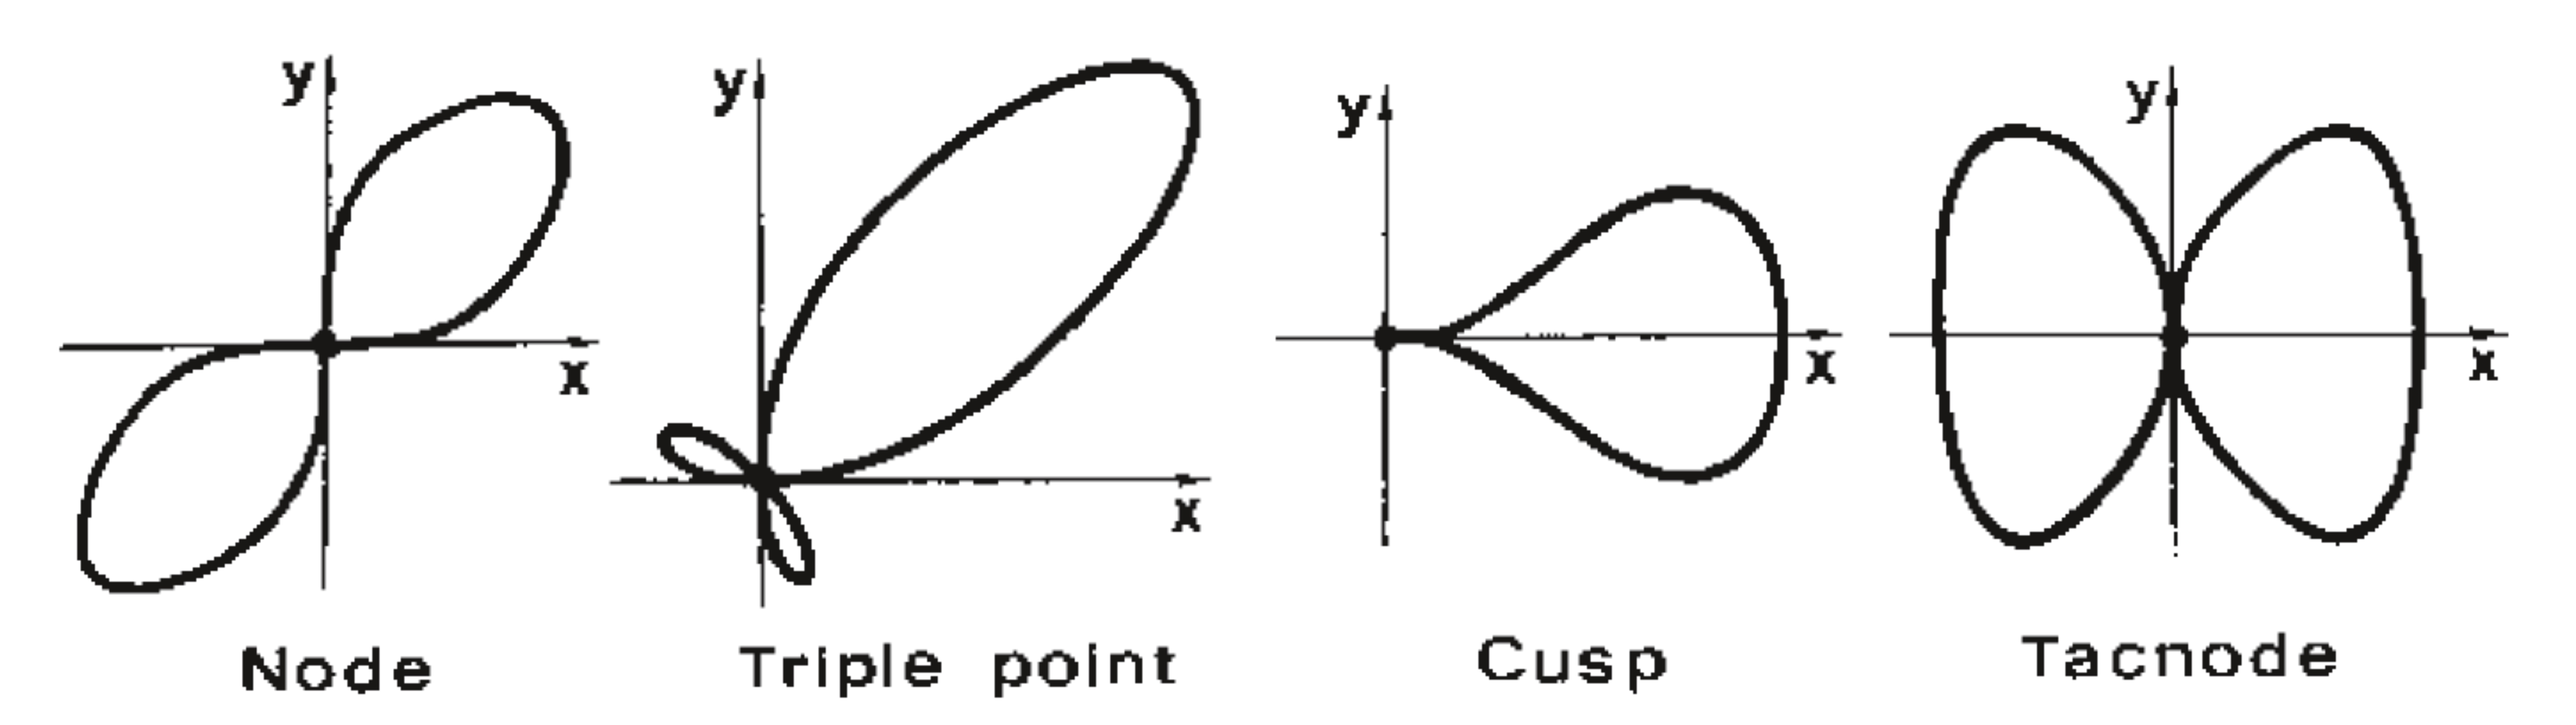
\includegraphics[width=0.8\columnwidth]{Figure4}\\
	Figure 4. 평면 곡선의 특이점
	\end{center}
	%
	\begin{enumerate}[label=,itemindent=0mm]
	\item Sol) Figure 4의 네 곡선은 차례대로 (b), (d), (c), (a)이다. 특이점은 모두 원점이다.\\
	\end{enumerate}
	%
	\begin{enumerate}[label=\tb{5.\arabic*.},itemindent=0mm,itemsep=4mm]
	\setcounter{enumi}{1}
	\item 다음과 같은 $\mb A^3$에서의 곡면들의 특이점의 위치를 찾고 특이점을 기술하라. ($\Char k\ne 2$라 가정하라.)
	각각의 방정식에 대응하는 곡선은 Figure 5에서 어떤 것인가?
	\begin{enumerate}[label=(\alph*)]
	\item $xy^2=z^2$
	\item $x^2+y^2=z^2$
	\item $xy+x^3+y^3=0$
	\end{enumerate}
	\end{enumerate}
	%
	%Figure 5
	\begin{center}
	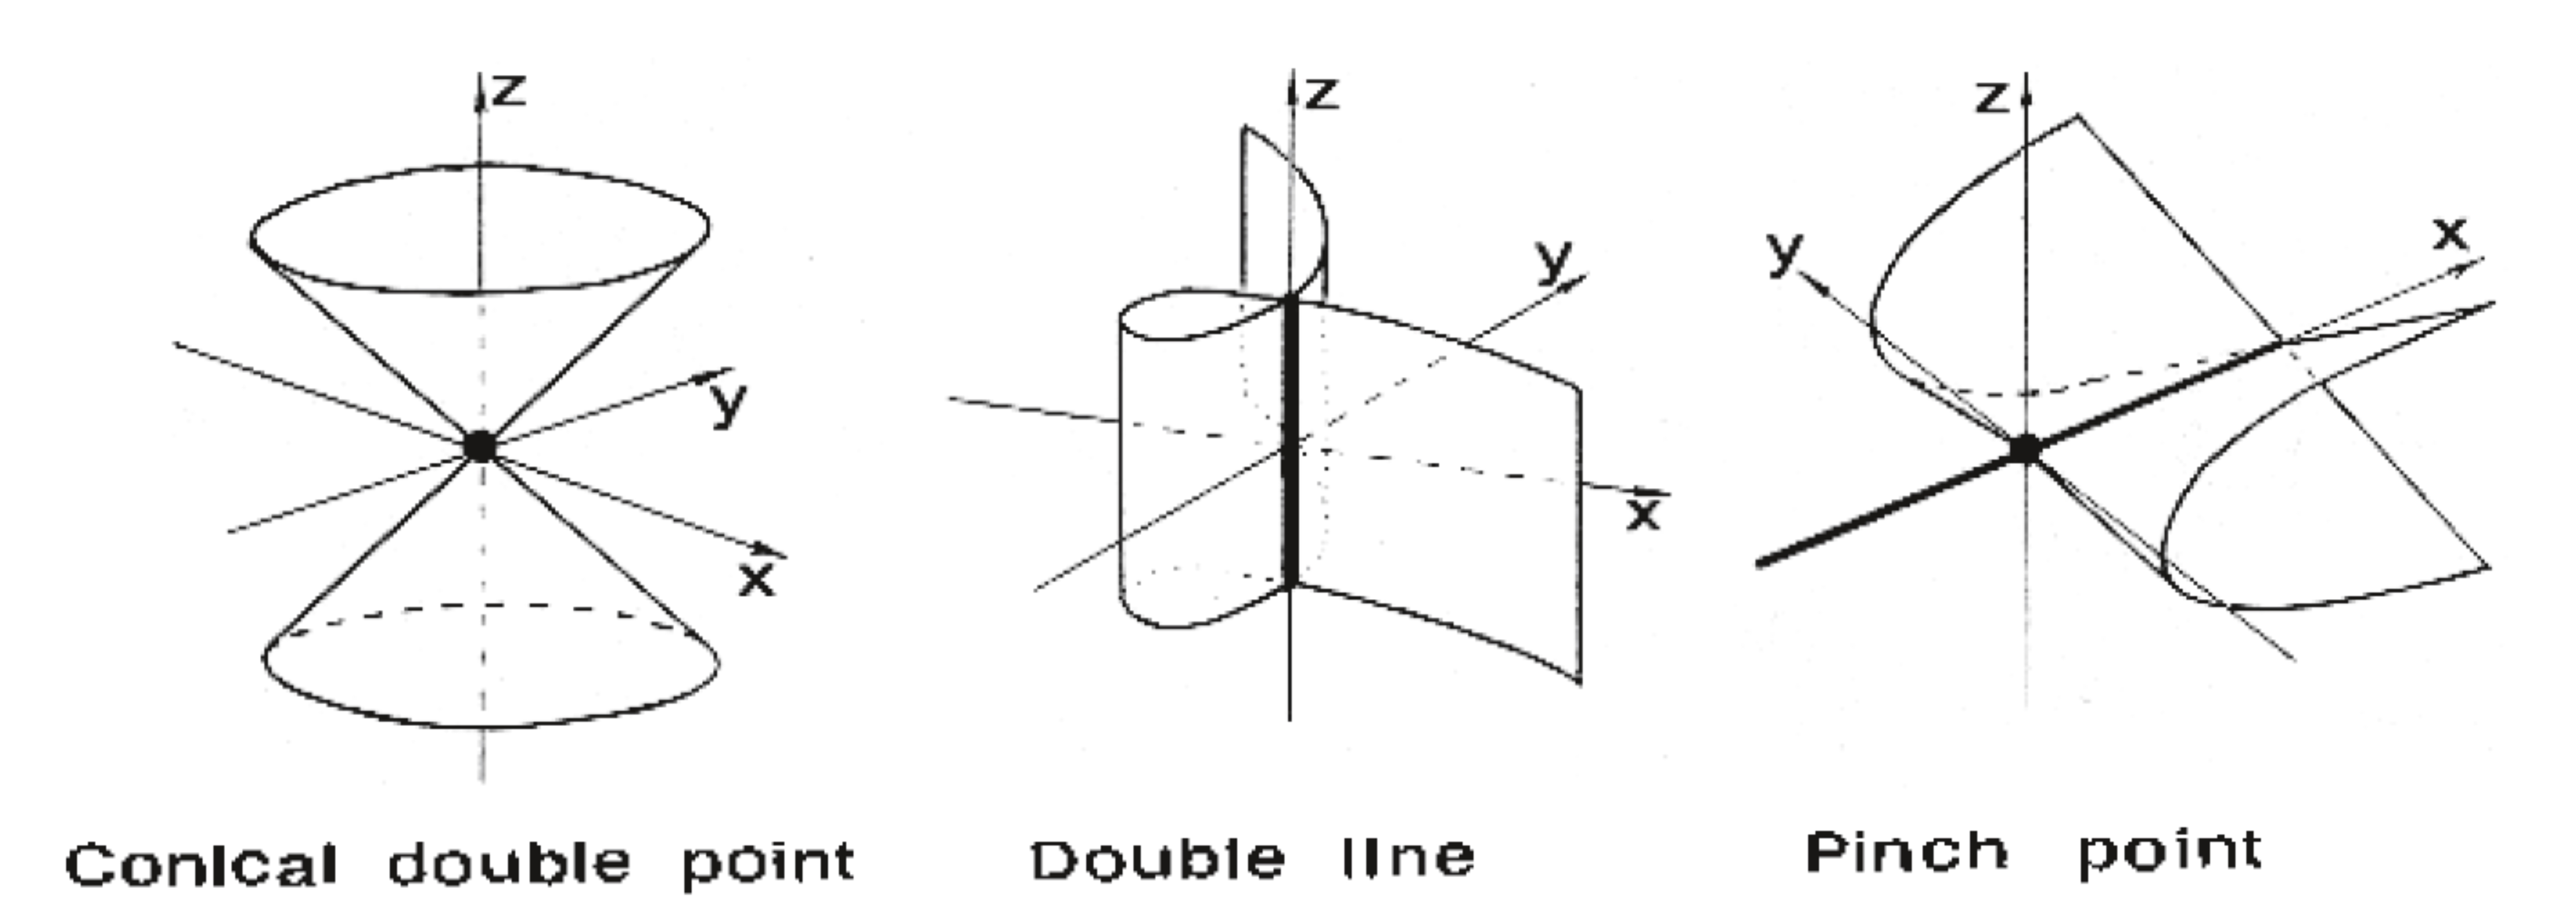
\includegraphics[width=0.8\columnwidth]{Figure5}\\
	Figure 5. 곡면 특이점
	\end{center}
	%
	\begin{enumerate}[label=,itemindent=0mm]
	\item Sol) Figure 5의 세 곡면은 순서대로 (b), (c), (a)이다. (a)의 특이점들은 $x$축, (b)의 특이점은 원점,
	(c)의 특이점들은 $z$축이다.\\
	\end{enumerate}
	%
	\begin{enumerate}[label=\tb{5.\arabic*.},itemindent=0mm,itemsep=4mm]
	\setcounter{enumi}{2}
	\item \tb{중복도.} $Y\bseq\mb A^2$가 방정식 $f(x,y)=0$에 의해 정의된 곡선이라 하자. $P=(a,b)$가 $\mb A^2$의 점이라 하자.
	좌표계를 1차다항식에 의해 변환하여 $P$가 점 $(0,0)$이 되도록 하자.
	그 후 $f$를 $x$와 $y$에 대한 $i$차 동차다항식 $f_i$들의 합 $f=f_0+f_1+\cdots+f_d$로 표현하자.
	$P$의 $Y$ 상에서의 \tb{중복도(multiplicity)}를 $f_r\ne 0$이도록 하는 최소 $r$로 정의하고 $\mu_P(T)$로 표기하자.
	($P\in Y\Lra\mu_P(Y)>0$임을 기억해 두라.) $f_r$의 선형 인수들은 $P$에서의 \tb{접선방향(tangent direction)}들이라 불린다.
	\begin{enumerate}[label=(\alph*)]
	\item $\mu_P(T)=1\Lra P$가 $Y$의 비특이점인 것임을 보여라.
	\item 위의 (Ex. 5.1)에 있는 각각의 특이점들의 중복도를 찾아라.
	\end{enumerate}
	%
	\sol (a) $f_1=\al x+\be y$라 하면 $\pa_xf(0,0)=\al,\pa_yf(0,0)=\be$이므로
	$f_r\ne 0$ iff $f$의 $(0,0)$에서의 Jacobian이 계수 1을 가짐 iff $P$가 비특이점인 것이다.\\
	(b) (Ex. 5.1)의 (a), (b), (c)의 특이점은 중복도 2이며 (d)의 특이점은 중복도 3이다.
	%
	\item \tb{교차 중복도.} 만약 $Y,Z\bseq\mb A^2$가 서로 다른 두 곡선이며 방정식 $f=0,g=0$에 의해 주어지고 만약 $P\in Y\cap Z$이면
		$Y$와 $Z$의 $P$에서의 \tb{교차 중복도(intersection multiplicity)} $(Y\cdot Z)_P$를
		$\mc O_P$-모듈 $\mc O_P/(f,g)$의 길이로 정의한다.
		\begin{enumerate}[label=(\alph*)]
			\item $(Y\cdot Z)_P$가 유한하며 $(Y\cdot Z)_P\ge\mu_P(Y)\cdot\nu_P(Z)$임을 보여라.
			\item 만약 $P\in Y$이면 $P$를 통과하는 거의 모든(i.e. 유한 개를 제외한 모든) 직선 $L$에 대하여 $(L\cdot Y)_P=\mu_P(Y)$임을 보여라.
			\item 만약 $Y$가 $\mb P^2$에서의 $d$차곡선이며 $L$이 $\mb P^2$에서의 직선이고 $L\ne Y$이면 $(L\cdot Y)=d$임을 보여라.
			여기에서 $(L\cdot Y)=\sum(L\cdot Y)_P$(모든 점 $P\in L\cap Y$에 대한 합)로 정의하며
			$(L\cdot Y)_P$는 $\mb P^2$의 적절한 아핀 덮개를 이용하여 정의된다.
		\end{enumerate}
	\item 모든 차수 $d>0$과 $p=0$ 또는 임의의 소수 $p$에 대하여 표수 $p$의 체 $k$ 상에서의
	$\mb P^2$에서의 비특이 $d$차곡선의 방정식을 제시하라.
	\item \tb{곡선 특이점의 부풀림.}
	\begin{enumerate}[label=(\alph*)]
	\item $Y$가 (Ex. 5.1)의 첨점 또는 결절점을 가지는 곡선이라 하자.
	$Y$를 $O=(0,0)$에서 부풀려 얻어진 곡선 $\tilde Y$는 비특이이다. (cf. (4.9.1)과 (Ex. 4.10))
	\item \tb{결절점(node)}(또는 \tb{통상2중점(ordinary double point)})을 서로 다른 접선방향(Ex. 5.3)들을 가지는
	평면 곡선의 2중점(i.e. 중복도 2의 점)으로 정의한다.
	만약 $P$가 평면 곡선 $Y$ 상에서의 결절점이면 $\ph^{-1}(P)$가 부풀려진 곡선 $\tilde Y$ 상에서의
	서로 다른 두 개의 비특이점들로 구성됨을 보여라. 우리는 `$P$를 부풀리는 것이 $P$에서의 특이점을 해소한다'고 말한다.
	\item $P\in Y$가 (Ex. 5.1)의 접촉절점이라 하자.
	만약 $\ph:\tilde Y\ra Y$가 $P$에서의 부풀림이면 $\ph^{-1}(P)$가 ($\Char k\ne 2$인 경우) 결절점임을 보여라.
	(b)를 이용하면 우리는 접촉절점이 2회의 순차적인 부풀림에 의해 해소될 수 있음을 알 수 있다.
	\item $Y$가 평면 곡선 $y^3=x^5$라 하자. 이는 $O$에서 `고차 첨점'을 가진다.
	$O$가 3중점임을 보여라; $O$를 부풀리는 것은 2중점을 제공한다. (어떠한 형태의 2중점인가?) 한 번 더 부풀리면 특이점이 해소된다.
	\end{enumerate}
	\ti{Note}: 우리는 나중에 (V, 3.8) 평면 곡선의 임의의 특이점이 유한 회의 순차적인 부풀림에 의해 해소될 수 있음을 보일 것이다.\\
	%
	\sol (a) (i) (Ex. 5.1)에서 첨점을 가지는 곡선은 $x^3-x^4=y^2+y^4$이다. 이를 원점에서 부풀리자.
	아핀 열린집합 $t=1$에서 $xu=y$와 $x=0$ 또는 $x^2(u^4+1)-x+u^2=0$을 얻는다.
	이곳에서 $E$와 $\tilde Y$의 교점은 $(x,y,u)=(0,0,0)$ 하나이다.
	$(0,0,0)$에서의 Jacobi 행렬 $\left(\begin{array}{ccc}0&1&0\\-1&0&0\end{array}\right)$가
	계수 $2=\codim Y$를 가지므로 $(0,0,0)$은 $\tilde Y$의 특이점이 아니다.
	아핀 열린집합 $u=1$에서 $x=ty$와 $y=0$ 또는 $y^2(1+t^4)-yt^3+1=0$을 얻는다.
	이곳에서는 $E$와 $\tilde Y$의 교점이 없다. 따라서 $\tilde Y$는 비특이이다.\\
	(ii) (Ex. 5.1)에서 결절점을 가지는 곡선은 $xy=x^6+y^6$이다. 이를 원점에서 부풀리자.
	아핀 열린집합 $t=1$에서 $xu=y$와 $x=0$ 또는 $x^4(1+u^6)-u=0$을 얻는다. Jacobi 행렬은 다음과 같다.
	%
	$$\left(\begin{array}{ccc}u&-1&x\\4x^3(1+u^6)&0&6x^4u^5-1\end{array}\right)$$
	%
	이는 $\tilde Y$의 모든 점에서 계수 2를 가진다. $u=1$에서도 동일하게 계산하면 $\tilde Y$가 비특이임이 따라온다.\\
	(b) (1차다항식에 의한 적절한 좌표변환을 거친 후) $Y$를 정의하는 다항식 $f$는 $xy+f_{3+}(x,y)$이다.
	($f_{3+}\sum_{n\ge 3}f_n$은 3차 이상의 항만 가지는 다항식이다.) 원점에서 이를 부풀리자.
	$g(x,u)=x^{-2}f_{3+}(x,xu)$라 하자. (이러한 $g$는 $x$에 대하여 1차 이상의 항만 가지는 다항식이다.)
	아핀 열린집합 $t=1$에서 $xu=y$와 $x=0$ 또는 $u+g(x,u)=0$을 얻는다.
	따라서 $t=1$ 내에서 $E$와 $\tilde Y$의 교점은 $(x,y,t,u)=(0,0,1,0)$ 하나이다.
	Jacobian은 $\left(\begin{array}{ccc}0&-1&0\\a&0&1\end{array}\right)$로 계수 2를 가진다. 따라서 $(0,0,1,0)$은 비특이점이다.
	마찬가지로 $u=1$에서 교점은 비특이점 $(0,0,0,1)$ 하나이다. 즉 $\ph^{-1}(P)$는 서로 다른 두 비특이점들로 구성된다.\\
	(c) (Ex. 5.1)에서 접촉절점을 가지는 곡선은 $x^2=x^4+y^4$이다. 이를 원점에서 부풀리자.
	아핀 열린집합 $t=1$에서 $xu=y$와 $x=0$ 또는 $1=x^2(1+u^2)$를 얻는다.
	따라서 $t=1$에서 $E$와 $\tilde Y$는 교차하지 않는다.
	아핀 열린집합 $u=1$에서 $x=ty$와 $y=0$ 또는 $t^2=y^2(t^4+1)$를 얻는다.
	따라서 $u=1$에서 $E$와 $\tilde Y$는 한 점 $(x,y,t)=(0,0,0)$에서 교차한다.
	$\tilde Y$를 평면 $x=ty$에서의 곡선으로 간주하면 위 교점에서 $f_2=y^2-t^2=(y-t)(y+t)$이므로 $\Char k\ne 2$인 경우 결절점이다.
	($\Char k=2$인 경우 $y+t=yt^2$이므로 비특이점이다.) (b)에 의해 이는 추가적인 부풀림에 의해 해소될 수 있다.\\
	(d) $f_1=f_2=0,f_3=y^3\ne 0$이므로 $Y$는 $O$에서 3중점을 가진다. 이를 $O$에서 부풀리자.
	아핀 열린집합 $u=1$에서 $x=ty$와 $y=0$ 또는 $1=t^5y^2$를 얻는다. 따라서 $u=1$에서 $E$와 $\tilde Y$는 교차하지 않는다.
	아핀 열린집합 $t=1$에서 $xu=y$와 $x=0$ 또는 $u^3=x^2$를 얻는다.
	따라서 $t=1$에서 $E$와 $\tilde Y$는 한 점 $(x,y,u)=(0,0,0)$에서 교차한다.
	$\tilde Y$를 평면 $xu=y$에서의 곡선으로 간주하면 $(x,u)=(0,0)$은 첨점이다.
	(a) (i)과 마찬가지 방식으로 부풀림을 통해 첨점을 해소할 수 있다.
	%
	\item $Y\bseq\mb P^2$가 방정식 $f(x,y,z)=0$에 의해 정의된 1차 초과의 비특이 평면 곡선이라 하자.
	$X\bseq\mb A^3$이 $f$에 의해 정의된 아핀 대수다양체라 하자. (이는 $Y$ 상에서의 뿔이다; (Ex. 2.10)을 참조하라.)
	$P$가 뿔의 \tb{꼭짓점(vertex)}인 점 $(0,0,0)$이라 하자. $\ph:\tilde X\ra X$가 $X$의 $P$에서의 부풀림이라 하자.
	\begin{enumerate}[label=(\alph*)]
	\item $X$가 하나의 특이점 $P$만을 가짐을 보여라.
	\item $\tilde X$가 비특이임을 보여라. (이를 아핀 열린집합들로 덮어라.)
	\item $\ph^{-1}(P)$가 $Y$와 동형임을 보여라.
	\end{enumerate}
	\item $Y\bseq\mb P^n$이 $r$차원 사영 대수다양체라 하자.
	$f_1,\ldots,f_t\in S=k[x_0,\ldots,x_n]$이 $Y$의 아이디얼을 생성하는 동차다항식들이라 하자.
	$P\in Y$가 동차 좌표 $P=(a_0,\ldots,a_n)$을 가지는 점이라 하자.
	$P$가 $Y$ 상에서 비특이일 필요충분조건은 행렬 $\|(\pa f_i/\pa x_j)(a_0,\ldots,a_n)\|$의 계수가 $n-r$인 것임을 보여라.
	[Hint: (a) 이러한 계수가 $P$에 대하여 선택된 동차 좌표에 독립적임을 보여라.
	(b) $P$를 포함하는 아핀 열린집합 $U_i\bseq\Pn$으로 보내고 아핀 Jacobi 행렬을 사용하라.
	(c) $f$가 $d$차 동차이면 $\sum x_i(\pa f/\pa x_i)=d\cdot f$라는 Euler 보조정리가 필요할 것이다.]\\
	%
	\sol $f_i$의 차수를 $d_i$로 표기하면 동차 좌표의 $a$배는 Jacobi 행렬의 $i$행이 $a^{d_i-1}$배가 되는 효과를 준다.
	이는 행렬의 계수에 영향을 주지 않는다.
	일반성을 잃지 않고 $P\in U_0$라 하자. 좌표를 $x_0=1$이도록 선택하자.
	그 경우 $P$에서의 아핀 Jacobi 행렬 $J_A$는 사영 Jacobi 행렬 $J_P$ 1열($x_0$에 대한 편도함수들)이 제거된 것이다.
	Euler 보조정리에 의해 $\sum x_i(P)(\pa f/\pa x_i)(P)=d\cdot f(P)=0$이므로
	1열은 어떠한 경우에도 다른 열들의 선형 결합으로 표현 가능하다; 따라서 1열의 제거는 계수에 영향을 주지 않는다.
	국소환과 그 극대 아이디얼 $\mf m$은 열린 근방에만 영향을 받으므로 아핀 경우와 사영 경우에 동일하다.
	$\rank J_P=\rank J_A=n-\dim\mf m/\mf m^2$이므로 $P$가 비특이 iff $\dim\mf m/\mf m^2=r$ iff $\rank J_P=n-r$이다.
	%
	\item $f\in k[x,y,z]$가 동차다항식이고 $Y=Z(f)\bseq\mb P^2$가 $f$에 의해 정의된 대수적 집합이며
	모든 $P\in Y$에 대하여 $(\pa f/\pa x)(P),(\pa f/\pa y)(P),(\pa f/\pa z)(P)$ 중 적어도 하나가 0이라 하자.
	$f$가 기약(이며 따라서 $Y$가 비특이 대수다양체)임을 보여라. [Hint: (Ex 3.7)을 사용하라.]
	\item 대수다양체 $X$ 상에서의 점 $P$에 대하여 $\mf m$이 국소환 $\mc O_P$의 극대 아이디얼이라 하자.
	$X$의 $P$에서의 \tb{Zariski 접공간(Zariski tangent space)} $T_P(X)$를 $\mf m/\mf m^2$의 쌍대 $k$-벡터 공간으로 정의한다.
	\begin{enumerate}[label=(\alph*)]
	\item 임의의 점 $P\in X$에 대하여 $\dim T_P(X)\ge\dim X$이며 등호가 성립할 필요충분조건은 $P$가 비특이점인 것이다.
	\item 임의의 사상 $\ph:X\ra Y$에 대하여 자연스러운 유도 $k$-선형 사상 $T_P(\ph):T_P(X)\ra T_{\ph(P)}(Y)$가 존재한다.
	\item 만약 $\ph$가 포물선 $x=y^2$의 $x$축 상으로의 종방향 사영이면 원점에서의 접공간의 유도 사상 $T_0(\ph)$가 0 사상임을 보여라.
	\end{enumerate}
	\item \tb{$\mb P^3$에서의 타원 4차곡선.} $Y$가 방정식 $x^2-xz-yw=0$과 $yz-xw-zw=0$에 의해 정의된
	$\mb P^3$에서의 대수적 집합이라 하자. $P$가 점 $(x,y,z,w)=(0,0,0,1)$이며 $\ph$가 $P$에서 평면 $w=0$으로의 사영이라 하자.
	$\ph$가 $Y-P$와 평면 3차곡선 $y^2z-x^3+xz^2=0$에서 점 $(1,0,-1)$을 제외한 것 간의 동형사상을 유도함을 보여라.
	그 후 $Y$가 기약 비특이 곡선임을 보여라. 이는 $\mb P^3$에서의 \tb{타원 4차곡선(eliptic quartic curve)}이라 불린다.
	이것이 두 방정식에 의해 정의되었으므로 이는 완비 교집합의 또 다른 예시이다. (Ex. 2.17)\\
	%
	\sol $Y$를 정의하는 두 식에서 $w$를 소거하여 $x(x^2-z^2)=(x+z)yw=y^2z$를 얻는다.
	즉 $\ph(Y-P)$는 $y^2z-x^3+xz^2=0$의 부분집합이다.
	$w$는 $y\ne 0$인 경우에는 $(x-z)x/y$이고 $x+z\ne 0$인 경우에는 $yz/(x+z)$으로 복원될 수 있다;
	$y\ne 0,x+z\ne 0$이며 $y^2z-x^3+xz^2=0$이 성립한다면 이러한 두 가지 $w$가 동일하므로 역이 모순 없이 잘 정의된다.
	그러나 $y=x+z=0$인 경우, 즉 $(1,0,-1)$은 $\ph(Y-P)$에 속하지 않는다.
	($Z(y^2z-x^3+xz^2)=Y'$이라 표기하면) 이는 $\ph$가 $Y-P$와 $Y'-\{(1,0,-1)\}$ 간의 동형사상임을 보여준다.
	도함수 $(z^2,0,y^2)$가 0이 되지 않으므로 $Y'$은 비특이이다. 따라서 $Y$도 $P$ 이외의 가능한 특이점이 없다.
	$Y$의 $P$에서의 Jacobian은 다음과 같다:
	%
	$$\left(\begin{array}{cccc}2x-z&-w&-x&-y\\-w&z&y-w&-x-z\end{array}\right)(0,0,0,1)
	=\left(\begin{array}{cccc}0&-1&0&0\\-1&0&-1&0\end{array}\right)$$
	%
	이는 계수 2를 가진다. 따라서 $Y$는 비특이이다.\\
	$y^2z-x^3+xz^2=fg,\deg f\ne 0,\deg g\ne 0$이라 가정하면 Theorem 7.2에 의해 $f$와 $g$의 공통영점이 존재하며
	이 점에서 $\pa_{x_i}(fg)=(\pa_{x_i}f)g+f(\pa_{x_i}g)=0$이므로 비특이성에 모순이다. 따라서 $Y'$은 기약이다.
	기약 대수적 집합의 열린 부분집합은 조밀하므로 임의의 두 열린 부분집합이 교차하며 따라서 $Y'-\{(1,0,1)\}$은 연결이다.
	그러므로 이와 동형인 $Y$에서의 열린집합 $Y-P$도 연결이다. $Y$가 공집합이 아닌 서로 소 열린집합 $Y_1,Y_2$로 분할된다면
	(한 점 집합 $P$가 공집합이 아닌 열린집합을 포함하지 못하므로) $Y_1,Y_2$는 모두 $Y-P$와 교차하며 따라서 $Y-P$의 연결성에 모순이다.
	따라서 $Y$는 연결이다.\\
	임의의 연결 비특이 대수적 집합은 기약이며 따라서 비특이 대수다양체이다: 먼저 좌표환의 정의를 임의의 대수적 집합으로 확대하자.
	기약 성분이 2개 이상 존재한다 하자. 연결성에 의해 임의의 두 기약 성분은 교차한다. $x$가 2개 이상의 기약 성분의 교집합에 속한다 하자.
	비특이성에 의해 $\mc O_x$가 정칙 국소환이다. 정칙 국소환은 정역이다. (가환대수학 교재를 참조하라.)
	따라서 $\mc O_x$는 $(0)$을 유일한 극소 소 아이디얼로 가진다.
	$\mc O_x$의 극소 소 아이디얼들은 $x$를 포함하는 기약 성분들에 대응된다.
	이는 $x$가 2개 이상의 기약 성분에 속함에 모순이다. 따라서 주장이 증명된다.
	%
	\item \tb{2차초곡면.} $\Char k\ne 2$이며 $f$가 $x_0,\ldots,x_n$에 대한 2차 동차다항식이라 하자.
	\begin{enumerate}[label=(\alph*)]
	\item 좌표계를 적절한 1차다항식에 의해 변환하는 것으로 어떠한 $0\le r\le n$에 대하여
	$f$가 $f=x_0^2+\cdots+x_r^2=0$의 형태가 될 수 있음을 보여라.
	\item $f$가 기약일 필요충분조건은 $r\ge 2$인 것임을 보여라.
	\item $r\ge 2$라 가정하고 $Q$가 $f$에 의해 정의된 $\Pn$에서의 2차초곡면이라 하자.
	$Q$의 특이 자취 $Z=\Sing Q$가 $n-r-1$차원 \ti{선형} 대수다양체(Ex. 2.11)임을 보여라.
	특히 $Q$가 비특이일 필요충분조건은 $r=n$인 것이다.
	\item $r<n$인 경우 $Q$는 축이 $Z$인 비특이 2차초곡면 $Q'\bseq\mb P^r$ 상에서의 뿔임을 보여라.
	(이러한 뿔의 개념은 (Ex. 2.10)에서 정의된 것의 일반화이다. 만약 $Y$가 $\mb P^r$의 닫힌 부분집합이며
	$Z$가 $\Pn$에서의 $n-r-1$차원 선형 부분공간이면 $\mb P^r$을 $\Pn$에 매장하여 $\mb P^r\cap Z=\es$이도록 하고
	\tb{축이 $Z$인 $Y$ 상에서의 뿔(cone over $Y$ with axis $Z$)}를 $Y$의 점과 $Z$의 점을 통과하는 모든 직선들의 합집합으로 정의한다.)
	\end{enumerate}
	\item 모든 정칙 국소환은 정수적으로 닫힌 정역이다. (Matsumura [2, Th. 36, p. 121])
	그러므로 (5.3)에 의해 임의의 대수다양체는 정규점들의 공집합이 아닌 열린 부분집합을 가짐을 알 수 있다. (Ex. 3.17)
	이 연습문제에서 ((5.3)을 사용하지 않고) 대수다양체의 비정규점들의 집합이 닫힌 진부분집합임을 보여라.
	(정수적 폐포의 유한성이 필요할 것이다: (3.9A)를 참조하라.)
	\item \tb{해석적 동형 특이점.}
	\begin{enumerate}[label=(\alph*)]
	\item 만약 $P\in Y$와 $Q\in Z$가 해석적 동형 평면 곡선 특이점이면 중복도 $\mu_P(Y)$와 $\mu_Q(Z)$가 동일함을 보여라. (Ex. 5.3)
	\item 본문의 예시 (5.6.3)을 일반화하여 만약 $f=f_r+f_{r+1}+\cdots\in k[[x,y]]$이며
	$f$의 최고차 형식 $f_r$이 $f_r=g_sh_t$로 분해되고 $g_s,h_t$가 각각 $s$차와 $t$차 동차이며
	공통 1차 인수를 갖지 않으면 $k[[x,y]]$에서의 형식적 멱급수
	%
	\begin{align*}
	g&=g_s+g_{s+1}+\cdots\\h&=h_t+h_{t+1}+\cdots
	\end{align*}
	%
	가 존재하여 $f=gh$를 만족시킨다.
	\item $Y$가 $\mb A^2$에서 방정식 $f(x,y)=0$에 의해 정의되며 $P=(0,0)$이 $Y$ 상에서의 중복도 $r$인 점이고
	따라서 $f$가 $x$와 $y$에 대한 다항식으로 전개되었을 경우 $f=f_r+$고차항 형태이다.
	$P$가 \tb{통상$r$중점(ordinary $r$-fold point)}임을 $f_r$이 서로 다른 $r$개 선형 인수들의 곱인 것으로 정의한다.
	임의의 두 통상2중점이 해석적 동형임을 보여라. 통상3중점에 대해서도 위와 같다.
	그러나 서로 동형이 아닌 통상4중점들의 1매개변수족이 존재함을 보여라.
	\end{enumerate}
		\begin{enumerate}[label=*(\alph*)]
			\setcounter{enumii}{3}
			\item $\Char k\ne 2$라 가정하자. 평면곡선의 임의의 2중점들이 유일하게 결정된 $r\ge 2$에 대하여
			곡선 $y^2=x^r$의 $(0,0)$에서의 특이점과 해석적 동형임을 보여라.
			만약 $r=2$이면 이는 결절점이다. (Ex. 5.6) 만약 $r=3$이면 이는 \tb{첨점(cusp)}이다;
			만약 $r=4$이면 \tb{접촉절점(tacnode)}이다. 심화된 논의를 위해서는 (V, 3.9.5)를 참조하라.
		\end{enumerate}
		\item \tb{평면 곡선들의 족.} 3변수 $x,y,z$에 대한 $d$차 동차다항식 $f$는 $\binom{d+2}2$개 계수들을 가진다.
		이러한 계수들이 $N=\binom{d+2}2-1=\fra 2d(d+3)$인 $\mb P^N$에서의 점을 표현한다 하자.
		\begin{enumerate}[label=(\alph*)]
			\item 이것이 $\mb P^N$의 점들과 $d$차방정식에 의해 정의될 수 있는 $\mb P^2$의 대수적 집합들 간의 대응 관계를 제공함을 보여라.
			$f$가 다수의 인자를 가지는 몇 가지 경우를 제외하면 이러한 대응이 일대일임을 보여라.
			\item 이러한 대응 하에서 (기약) 비특이 $d$차곡선들이 $\mb P^N$의 공집합이 아닌 Zariski-열린 부분집합의 점들에
			일대일 대응됨을 보여라. [Hint: (1) 동차다항식 $\pa f/\pa x_0,\ldots,\pa f/\pa x_n$에 적용된 소멸 이론 (5.7A)를 사용하라.
			(2) 위의 (Ex. 5.5, 5.8, 5.9)를 사용하라.]
		\end{enumerate}
	\end{enumerate}
	
	
	
	\subsection*{Section I.6}
	
	\begin{enumerate}[label=\tb{6.\arabic*.},itemindent=0mm,itemsep=4mm]
		\item \tb{유리(rational)} 곡선이 $\mb P^1$과 쌍유리동치인 곡선임을 상기하라. (Ex. 4.4)
		$Y$가 $\mb P^1$과 동형이 아닌 비특이 유리곡선이라 하자.
		\begin{enumerate}[label=(\alph*)]
			\item $Y$가 $\mb A^1$의 열린 부분집합과 동형임을 보여라.
			\item $Y$가 아핀임을 보여라.
			\item $A(Y)$가 유일 인수분해 정역임을 보여라.
		\end{enumerate}
		\item \tb{타원곡선.} $Y$가 $\mb A^2$에서의 곡선 $y^2=x^3-x$라 하고 기반체 $k$의 표수가 2가 아니라 하자.
		이 연습문제에서 우리는 $Y$가 유리 곡선이 아니며 따라서 $K(Y)$가 $k$의 순수히 초월적 확대가 아님을 보일 것이다.
		\begin{enumerate}[label=(\alph*)]
			\item $Y$가 비특이임을 보이고 $A=A(Y)\cong k[x,y]/(y^2-x^3+x)$가 정수적으로 닫힌 정역임을 연역하라.
			\item $k[x]$가 $x$의 $A$에서의 상에 의해 생성된 $K=K(Y)$의 부분환이라 하자.
			$k[x]$가 다항식환이며 $A$가 $k[x]$의 $K$에서의 정수적 폐포임을 보여라.
			\item 자기동형사상 $\si:A\ra A$가 존재하여 $y$를 $-y$로 대응시키며 $x$를 고정함을 보여라.
			임의의 $a\in A$에 대하여 $a$의 \tb{노름(norm)}을 $N(a)=a\cdot\si(a)$로 정의하자.
			$N(a)\in k[x],N(1)=1$이며 임의의 $a,b\in A$에 대하여 $N(ab)=N(a)\cdot N(b)$임을 보여라.
			\item 노름을 사용하여 $A$에서의 가역원들이 정확히 $k$의 0이 아닌 원소들임을 보여라.
			$x$와 $y$가 $A$의 기약원임을 보여라. $A$가 유일 인수분해 정역이 \ti{아님}을 보여라.
			\item $Y$가 유리 곡선이 아님을 보여라. (Ex. 6.1)
			이러한 중요한 결과의 다른 증명을 위해서는 (II, 8.20.3)과 (III, Ex. 5.3)을 참조하라.
		\end{enumerate}
		\item (a) $\dim X\ge 2$ 또는 (b) $Y$가 사영 대수다양체가 아니면 (6.8)의 결과가 거짓임을 반례를 통해 보여라.
		\item $Y$가 비특이 사영 곡선이라 하자. 상수함수가 아닌 $Y$ 상에서의 모든 유리함수가 전사 사상 $\ph:Y\ra\mb P^1$을 정의하며
		모든 $P\in\mb P^1$에 대하여 $\ph^{-1}(P)$가 유한집합임을 보여라.
		\item $X$가 비특이 사영 곡선이라 하자. $X$가 대수다양체 $Y$의 (국소 닫힌) 부분다양체라 하자. (Ex. 3.10)
		$X$가 사실 $Y$의 닫힌 부분집합임을 보여라. 일반화를 위해서는 (II, Ex. 4.4)를 참조하라.
		\item \tb{$\mb P^1$의 자기동형사상.} $\mb P^1$을 $\mb A^1\cup\{\infty\}$로 간주하자.
		그 경우 $\mb P^1$의 \tb{선형 분수 변환(fractional linear transformation)}을
		$a,b,c,d\in k,ad-bc\ne 0$에 대하여 $x\mt(ax+b)/(cx+d)$로 대응시키는 것으로 정의하자.
		\begin{enumerate}[label=(\alph*)]
			\item 선형 분수 변환이 $\mb P^1$의 \tb{자기동형사상(automorphism)}(i.e. $\mb P^1$과 자기 자신의 동형사상)을 유도함을 보여라.
			이러한 모든 선형 분수 변환들의 군을 $\mrm{PGL}(1)$로 표기할 것이다.
			\item $\Aut\mb P^1$이 $\mb P^1$의 모든 자기동형사상들의 군을 나타낸다 하자.
			$\Aut\mb P^1\simeq\Aut k(x)$(체 $k(x)$의 $k$-자기동형사상들의 군)임을 보여라.
			\item 이제 $k(x)$의 모든 자기동형사상이 선형 분수 변환임을 보이고 $\mrm{PGL}(1)\ra\Aut\mb P^1$이 동형사상임을 연역하라.
		\end{enumerate}
		\ti{Note}: 우리는 나중에(II, 7.1.1) 유사한 결과가 $\Pn$에 대하여 성립함을 보일 것이다:
		모든 자기동형사상은 도앛 좌표들의 선형 변환에 의해 주어진다.
		\item $P_1,\ldots,P_r,Q_1,\ldots,Q_s$가 $\mb A^1$의 서로 다른 점들이라 하자.
		만약 $\mb A^1-\{P_1,\ldots,P_r\}$이 $\mb A^1-\{Q_1,\ldots,Q_s\}$와 동형이면 $r=s$임을 보여라. 역이 참인가? cf. (Ex. 3.1)
	\end{enumerate}
	
	
	
	\subsection*{Section I.7}
	
	\begin{enumerate}[label=\tb{7.\arabic*.},itemindent=0mm,itemsep=4mm]
	\item \begin{enumerate}[label=(\alph*)]
	\item $\Pn$의 $\mb P^N$으로의 $d$차 매장(Ex. 2.12)의 차수를 찾아라. [답: $d^n$]
	\item $\mb P^r\times\mb P^s$의 $\mb P^N$으로의 Segre 매장(Ex. 2.14)의 차수를 찾아라. [답: $\binom{r+s}r$]
	\end{enumerate}
	%
	\sol (a) (Ex. 2.12)에 의해 동차 좌표환은 등급 대수로서 $d$차 단항식들에 의해 생성된 $k[x_0,\ldots,x_n]$의 부분대수와 동형이다.
	그러므로 $l$급 원소들은 $x_i$들에 대한 $dl$차 동차다항식들이며 따라서 $\ph_Y(l)={}_{n+1}H_{dl}=\binom{n+dl}{n}$이다.
	그러므로 $P_Y(z)=\binom{n+dz}n$이며 따라서 차수는 $n!\cdot\frac{d^n}{n!}=d^n$이다.\\
	(b) (Ex. 2.14)에 의해 동차 좌표환은 등급 대수로서 $x_iy_k$들에 의해 생성된
	$k[x_0,\ldots,x_r,y_0,\ldots,y_s]$의 부분대수와 동형이다.
	그러므로 $l$급 원소들은 $x_i$에 대하여 $l$차 동차, $y_i$에 대하여 $l$차 동차인 다항식들이며
	따라서 $\ph_Y(l)=\binom{r+l}l\binom{r+l}l=\binom{r+l}{r}\binom{s+l}s$이다.
	그러므로 $P_Y(z)=\binom{r+z}r\binom{s+z}s$이며 따라서 차수는 $(r+s)!\cdot\fra{r!s!}=\binom{r+s}r$이다.
	%
	\item $Y$가 $\Pn$에서의 $r$차원 대수다양체이며 Hilbert 다항식 $P_Y$를 가진다 하자.
	$Y$의 \tb{산술종수(arithmetic genus)}를 $p_a(Y)=(-1)^r(P_Y(0)-1)$로 정의하자.
	이는 $Y$의 사영 매장에 독립적인 중요한 불변량이다. (나중에 이를 (III, Ex. 5.3)에서 보게 될 것이다.)
	\begin{enumerate}[label=(\alph*)]
	\item $p_a(\Pn)=0$임을 보여라.
	\item 만약 $Y$가 평면 $d$차곡선이면 $p_a(Y)=\fra 2(d-1)(d-2)$임을 보여라.
	\item 더 일반적으로 만약 $H$가 $\Pn$에서의 $d$차 초곡면이면 $p_a(H)=\binom{d-1}n$이다.
	\item 만약 $Y$가 $\mb P^3$에서의 차수 $a,b$인 곡면들의 완비 교집합이면 (Ex. 2.17)
	$p_a(Y)=\fra 2ab(a+b-4)+1$이다.
	\item $Y^r\bseq\Pn,Z^s\bseq\mb P^m$이 사영 대수다양체라 하고
	$Y\times Z\bseq\Pn\times\mb P^m\ra\mb P^N$으로 Segre 매장에 의해 매장하자. 다음이 성립함을 보여라.
	%
	$$p_a(Y\times Z)=p_a(Y)p_a(Z)+(-1)^sp_a(Y)+(-1)^rp_a(Z)$$
	%
	\end{enumerate}
	%
	\sol (a) $\Pn$에 대하여 $\ph_{\Pn}(l)=\binom{n+l}n,P_{\Pn}(z)=\binom{n+z}n$, 차수 $n!\fra{n!}=1$이므로
	산술종수 $p_a(\Pn)=(-1)^n(1-1)=0$이다.\\
	(b) 평면 $d$차곡선은 단일한 $d$차 동차다항식 $f$에 의해 생성되며
	이러한 $f$는 동차 좌표환 내에서 $d$차 동차다항식들 간의 선형 종속 관계가 된다.
	따라서 $\ph_Y(l)$은 $l\le d$이면 $\binom{l+2}2$,
	$l\ge d$이면 $\binom{l+2}2-\binom{l-d+2}2$이다. ($f$를 인자로 가지는 다항식들 제외)
	그 경우 $P_Y(z)=\binom{z+2}2-\binom{z-d+2}2=\fra 2(z+2)(z+1)-\fra 2(z-d+2)(z-d+1)=zd-\frac{d^2-3d}2$이다.
	따라서 $P_Y(0)=-(d^2-3d)/2$이며 $p_a(Y)=(-1)(P_Y(0)-1)=(d-1)(d-2)/2$이다.\\
	(c) $d$차초곡면도 마찬가지로 단일한 $d$차 동차다항식에 의해 생성되므로 $\ph_Y(l)$은 $l\le d$이면 $\binom{l+n}n$,
	$l\ge d$이면 $\binom{l+n}n-\binom{l-d+n}n$이며 따라서 $P_Y(z)=\binom{z+n}n-\binom{z-d+n}n$이고
	$P_Y(0)=1+(-1)^{n+1}(d-n)\cdots(d-1)/n!$이다. 그러므로 $p_a(Y)=(-1)^{n-1}(P_Y(0)-1)=(d-1)\cdots(d-n)/n!=\binom{d-1}n$이다.\\
	(d) $Y=X_1\cap X_2,X_i=Z(f_i),\deg f_1=a,\deg f_2=b$라 하자. $X_1\cup X_2=Z(f_1f_2)$이므로 $\deg X_1\cup X_2=a+b$이다.
	다음의 완전열에 의해,
	%
	$$0\ra S/(f_1f_2)\ra S/(f_1)\oplus S/(f_2)\ra S/(f_1,f_2)\ra 0$$
	%
	$P_Y=P_{X_1}+P_{X_2}-P_{X_1\cup X_2}=\binom{z+3}3-\binom{z-a+3}3-\binom{z-b+3}3+\binom{z-a-b+3}3$이다.
	그러므로 $p_a(Y)=(-1)^1[\binom{3-a-b}3-\binom{3-a}3-\binom{3-b}3]=\fra 2ab(a+b-4)+1$이다.\\
	(e) $Y$와 $Z$의 동차 좌표환을 각각 $\bigoplus_iM_i\bseq k[x_0,\ldots,x_n]$과
	$\bigoplus N_i\bseq k[y_0,\ldots,y_m]$으로 분해하면
	$X\times Y$의 동차 좌표환은 $\bigoplus_iM_i\otimes N_i$와 동형이다. cf. (Ex. 2.14), (Ex. 7.1b).
	텐서곱의 차원은 곱인자의 차원의 곱이므로 $\ph_{Y\times Z}(l)=\ph_Y(l)\ph_Z(l)$이며 따라서 $\ph_{Y\times Z}=\ph_Y\ph_Z$이다.
	그러므로 $P_{Y\times Z}=P_YP_Z$이며 $p_a(Y\times Z)=(-1)^{r+s}(P_Y(0)P_Z(0)-1)
	=(-1)^{r+s}[(P_Y(0)-1)(P_Z(0)-1)+(P_Y(0)-1)+(P_Z(0)-1)]=p_a(Y)p_a(Z)+(-1)^sp_a(Y)+(-1)^rp_a(Z)$이다.
	%
		\item \tb{쌍대 곡선.} $Y\bseq\mb P^2$가 곡선이라 하자.
		직선 $L:a_0x_0+a_1x_1+a_2x_2=0$의 동차 좌표를 $(a_0,a_1,a_2)$로 취하여
		$\mb P^2$에 속한 직선들의 집합을 다른 사영공간 $(\mb P^2)^*$로 간주하자.
		각각의 비특이점 $P\in Y$에 대하여 유일한 직선 $T_P(Y)$가 존재하여 $Y$와의 $P$에서의 교차 중복도가 1 초과이도록 한다.
		이는 $Y$의 $P$에서의 \tb{접선(tangent line)}이다.
		함수 $P\mt T_P(Y)$가 $\mrm{Reg}\:Y$($Y$의 비특이점들의 집합)에서 $(\mb P^2)^*$로의 \ti{사상}을 정의함을 보여라.
		이 사상의 상의 폐포는 $Y$의 쌍대 곡선 $Y^*\bseq(\mb P^2)^*$라 불린다.
		\item $\mb P^2$에서의 $d$차 곡선 $Y$가 주어진 경우 $(\mb P^2)^*$의 Zariski 위상 하에서의 공집합이 아닌 열린 부분집합
		$U$가 존재하여 각각의 $L\in U$에 대하여 $L$이 $Y$와 정확히 $d$개 점에서 교차하도록 할 수 있다.
		[Hint: $Y$에 접하거나 또는 $Y$의 특이점을 지나는 $(\mb P^2)^*$에서의 직선들의 집합이 진부분집합에 포함됨을 보여라.]
		이 결과는 $Y$의 차수를 $\mb P^2$에서의 거의 모든 직선이 $Y$와 $d$개 점에서 만나도록 하는 수 $d$로 정의할 수 있었음을 보여준다.
		(여기에서 `거의 모든'은 쌍대 사영공간 $(\mb P^2)^*$와 동일시된 직선들의 집합의 공집합이 아닌 열린집합을 의미한다.)
		\item \begin{enumerate}[label=(\alph*)]
			\item $\mb P^2$에서의 $d>1$차 기약 곡선 $Y$는 중복도 $d$ 이상의 점을 가질 수 없음을 보여라. (Ex. 5.3)
			\item 만약 $Y$가 $d>1$차 기약 곡선이며 중복도 $d-1$인 점을 가지면 $Y$는 유리 곡선이다. (Ex. 6.1)
		\end{enumerate}
		\item \tb{선형 대수다양체.} 순수히 $r$차원인(i.e. 모든 기약 성분이 $r$차원인) 대수적 집합 $Y$가 차수 1을 가질 필요충분조건은
		$Y$가 선형 대수다양체(Ex. 2.11)인 것임을 보여라. [Hint: 먼저 (7.7)을 사용하여 $\dim Y=1$인 경우를 다루어라.
		그 후 초평면으로 자르고 귀납법을 사용하여 일반적인 경우를 다루어라.]
		\item $Y$가 $\Pn$에서의 차원 $r$이며 차수 $d>1$의 대수다양체라 하자. $P\in Y$가 비특이점이라 하자.
		$Q\in Y,Q\ne P$에 대하여 $X$를 모든 직선 $PQ$들의 합집합의 폐포로 정의하자.
		\begin{enumerate}[label=(\alph*)]
			\item $X$가 $r+1$차원 대수다양체임을 보여라.
			\item $\deg X<d$임을 보여라. [Hint: $\dim Y$에 대한 귀납법을 사용하라.]
		\end{enumerate}
		\item $Y^r\bseq\Pn$이 2차 대수다양체라 하자. $Y$가 $\Pn$에서의 $r+1$차원 선형 부분공간 $L$에 포함됨을 보여라.
		그러므로 $Y$는 $\mb P^{r+1}$에서의 2차초곡면과 동형이다. (Ex. 5.12)
	\end{enumerate}
	
	
	
	\section*{Chapter II}
	
	\subsection*{Section II.1}
	
	\begin{lemma*}
	%
		\tn{\\$\phi,\psi:\ms F\ra\ms G$가 위상공간 $X$ 상에서의 층 사상이며
		모든 $P\in X$에 대하여 $\phi_P=\psi_P$이면 $\phi=\psi$이다.\\\\
	%
		\pf 만약 $\phi(U)(s)\ne\psi(U)(s)$를 만족시키는 $U\bseq X$와 $s\in\ms F(U)$가 존재한다 가정하자.
		어떠한 $P\in U$에 대하여 $(\phi(U)(s))_P\ne(\psi(U)(s))_P$이다.
		(그렇지 않으면 각각의 점에 대하여 적당한 근방이 존재하여 그곳에서 $\phi(U)(s)=\psi(U)(s)$이므로 모순이다.)
		$(\phi(U)(s))_P=\phi_P(s_P),(\psi(U)(s))_P=\psi_P(s_P)$이므로 $\phi_P\ne\psi_P$이며 전제조건에 모순이다.}
	%
		\qed
	%
	\end{lemma*}
	
	\begin{enumerate}[label=\tb{1.\arabic*.},itemindent=0mm,itemsep=4mm]
	\item $A$가 가환군이라 하고 위상공간 $X$ 상에서 $A$에 연관된 \tb{상수 준층(constant presheaf)}을
	모든 $U\ne\es$에 대하여 $U\mt A$이며 제한함수가 항등사상인 준층으로 정의하자.
	본문에서 정의된 상수층 $\ms A$가 이러한 준층에 연관된 층임을 보여라.\\
	%
	\sol $A$에 연관된 상수 준층을 $\ms A_0$라 하고, $\ms A_0$에 연관된 층을 (1.2)에서와 같이 구축하자.
	모든 점 $P$에 대하여 줄기 $(\ms A_0)_P=A$이다. $\ms A_0^+(U)$는 다음을 만족시키는 함수 $s:U\ra A$들의 집합이다:
	각각의 $P\in U$에 대하여 $P$의 근방 $V\bseq U$와 원소 $t\in A$가 존재하여 모든 $Q\in V$에 대하여 $t=s(Q)$이다.
	따라서 원소 $s(P)=t$를 만족시키는 $P\in X$들의 집합은 열린집합이며
	그러므로 $s$는 $X$에서 이산위상이 부여된 $A$로의 함수로서 연속하다. 역으로 $s$가 연속하면 위 조건이 자명하게 성립한다.
	따라서 본문에서 정의한 상수층 $\ms A$는 $\ms A_0^+$와 일치한다.
	%
	\item \begin{enumerate}[label=(\alph*)]
	\item 임의의 층 사상 $\ph:\ms F\ra\ms G$에 대하여 각각의 점 $P$에 대하여
	$(\ker\ph)_P=(\ker\ph_P)$이며 $(\im\ph)_P=\im(\ph_P)$임을 보여라.
	\item $\ph$가 단사(resp. 전사)일 필요충분조건은 모든 $P$에 대하여
	줄기 상에서의 유도 함수 $\ph_P$들이 단사(resp. 전사)인 것임을 보여라.
	\item 층과 사상의 열 $\cdots\ms F^{i-1}\sr{\ph^{i-1}}\longra\ms F^i\sr{\ph^i}\longra\ms F^{i+1}\longra\cdots$가 완전열일
	필요충분조건이 각각의 $P\in X$에 대하여 대응하는 줄기의 열들이 가환군의 열로서 완전열인 것임을 보여라.
	\end{enumerate}
	%
	\sol (a) $s_P\in(\ker\ph)_P\Lra$ 어떠한 $P$의 근방 $U$와 $s\in\ker(\ph(U))\bseq\ms F(U)$가 존재하여 $s$가 $s_P$의 당김이다
	$\Lra s\in\ms F(U)$의 싹이 $s_P$이며 임의의 $V\bseq U$에 대하여 $\ph(V)(s\rest_V)=0\Lra\ph_P(s_P)=0\Lra s_P\in\ker(\ph_P)$.\\
	$s_P\in(\im\ph)_P\Lra$ 어떠한 $P$의 근방 $U$와 $s\in\im(\ph)(U)$가 존재하여 $s$가 $s_P$의 당김이다
	$\Lra t\in(\im(\ph(U)))$가 존재하여 $t$가 $s_P$의 당김이다
	$\Lra t_0\in\ms F(U)$가 존재하여 $\ph(t_0)=t$이며 $t$가 $s_P$의 당김이다 $\Lra s_P\in\im(\ph_P)$.\\
	(b) $\ker\ph=0\Lra\forall P\in X\:(\ker\ph)_P=0$ (층의 공리 (3)에 의해 $\La$ 방향이 성립) $\Lra\forall P\in X\ker(\ph_P)=0$,
	$\im\ph=\ms G\Lra\forall P\in X\:(\im\ph)_P=\ms G_P$ (층의 공리 (4)에 의해 $\La$ 방향이 성립)
	$\Lra\forall P\in X\:\im(\ph_P)=\ms G_P$\\
	(c) $\forall i\:\ker\ph^i=\im\ph^{i-1}\Lra\forall i\:\forall P\in X\:(\ker\ph^i)_P=(\im\ph^{i-1})_P$
	(층의 공리 (4)에서의 유일성에 의해 $\La$ 방향이 성립) $\Lra\forall i\:\forall P\in X\:\ker(\ph^i_P)=\im(\ph^{i-1}_P)
	\Lra\forall P\in X$에 대하여 가환군의 열 $\cdots\ms F^{i-1}_P\sr{\ph^{i-1}_P}\longra\ms F^i_P\sr{\ph^i_P}
	\longra\ms F^{i+1}_P\longra\cdots$가 완전열
	%
	\item \begin{enumerate}[label=(\alph*)]
	\item $\ph:\ms F\ra\ms G$가 $X$ 상에서의 층 사상이라 하자. $\ph$가 전사일 필요충분조건은 다음 조건이 성립하는 것이다:
	모든 열린집합 $U\bseq X$와 모든 $s\in\ms G(U)$에 대하여 $U$의 덮개 $\{U_i\}$와 원소 $t_i\in\ms F(U_i)$들이 존재하여
	모든 $i$에 대하여 $\ph(t_i)=s\rest_{U_i}$를 만족시킨다.
	\item 전사 층 사상 $\ph:\ms F\ra\ms G$과 $\ph(U):\ms F(U)\ra\ms G(U)$가 전사가 아니도록 하는 열린집합 $U$의 예를 제시하라.
	\end{enumerate}
	%
	\sol (a) $\ph$가 전사임은 모든 $\ph_P$가 전사임과 동치이다.\\
	($\La$) $P\in X,s_P\in\ms G_P$와 그 당김 $s\in\ms G(U)$를 선택하자.
	$U$의 덮개 $\{U_i\}$와 $t_i\in\ms F(U_i)$들이 존재하여 $\ph(t_i)=s\rest_{U_i}$를 만족시킨다.
	$P\in U_i$를 만족시키는 $i$에 대하여 $(t_i)_P=s_P$이다. 따라서 $\ph_P$가 전사이다.\\
	($\Ra$) $s\in\ms G(U)$를 선택하자. $\ph_P(t_P)=s_P$를 만족시키는 $t_P\in\ms F_P$들이 존재한다.
	따라서 모든 $P$에 대하여 ($t(P)$가 $t_P$의 임의의 당김이라 하면) $\ph(t(P)\rest_{V_P})=s\rest_{V_P}$를 만족시키는
	$P$의 근방 $V_P$가 존재한다. $U$의 열린 덮개 $\{V_P\}$와 $t(P)\rest_{V_P}$들은 주어진 조건을 만족시킨다.\\
	(b) $\mc O_\C$가 $\C$의 열린 부분집합 $U$에 $U$에서의 홀로모픽 함수들의 덧셈군을 대응시키는 홀로모픽 함수층이며
	$\mc O_\C^*$가 $\C$의 열린 부분집합 $U$에 $U$에서의 영점 없는 홀로모픽 함수들의 곱셈군을 대응시키는
	0이 아닌 홀로모픽 함수층이라 하자.
	$\ph:\mc O_\C\ra\mc O_\C^*,f\mt e^{2\pi if}$라 하자.
	충분히 작은 근방에서 모든 영점 없는 홀로모픽 함수는 로가리듬을 가지므로 임의의 $P$에 대하여 $\ph_P$는 전사이다.
	그러나 $U=\C^*$인 경우 $z$는 영점 없는 홀로모픽 함수이지만 대역적 로가리듬을 갖지 않으며 따라서 $\ph(U)$는 전사가 아니다.
	%
	\item \begin{enumerate}[label=(\alph*)]
	\item $\ph:\ms F\ra\ms G$가 준층 사상이며 각각의 $U$에 대하여 $\ph(U):\ms F(U)\ra\ms G(U)$가 단사라 하자.
	연관된 층 간의 유도 사상 $\ph^+:\ms F^+\ra\ms G^+$가 단사임을 보여라.
	\item (a)를 사용하여 만약 $\ph:\ms F\ra\ms G$가 층의 사상이면 본문에 언급된 것과 같이
	$\im\ph$가 $\ms G$의 부분층과 자연스럽게 동일시될 수 있음을 보여라.
	\end{enumerate}
	%
	\sol (a) 연관된 층의 정의에 의해 $\ms F_P=\ms F^+_P,\ms G_P=\ms G^+_P$이며 $\ph_P=\ph^+_P$이다.
	$\ph$가 단사이면 (Ex 1.2(b))에 의해 모든 $\ph_P=\ph_P^+$가 단사이며 따라서 $\ph^+$가 단사이다.\\
	(b) $\im_0$가 준층상을 나타낸다 하면 준층 사상으로 간주된 포함사상 $\io:\im_0(\ph)\ra\ms G$는 자명하게 단사이다.
	따라서 (a)에 의해 단사 층 사상 $\io^+:\im(\ph)\ra\ms G$가 존재하며 $\im(\ph)$를 $\ms G$의 부분층으로 간주할 수 있다.
	%
	\item 층의 사상이 동형사상일 필요충분조건은 단사이며 전사인 것임을 보여라.\\
	%
	\sol \tb{직접적인 해.} 층 사상 $\ph$에 대하여 각각의 $\ph(U)$의 역사상이 존재한다면 $\ph:U\mt(\ph(U))^{-1}$이
	층 사상의 정의에서의 가환 도표를 만족시킴이 자명하다.
	따라서 $\ph$가 동형사상일 필요충분조건은 각각의 $\ph(U)$의 역사상이 존재하는 것이다.
	즉 $\ker(\ph(U))=(\ker(\ph))(U)=0,\im(\ph(U))=\ms G(U)$인 것이다.
	전자의 조건은 단사성과 동치이다. 단사성이 성립할 경우 $\im(\ph(U))$는 $\ms F(U)$와 $\ph(U)$에 의해 동형이며
	$\ms F$가 층임에 의해 준층상 $\im_0(\ph)$도 층이다. 즉 준층상이 상과 같다.
	이러한 조건 하에서 전사성은 모든 $U$에 대하여 $\im\ph(U)=\ms G(U)$임과 동치이다.\\
	\tb{줄기에 의한 해.} Proposition 1.1과 (Ex 1.2(b))를 조합하면 따라온다.
	%
	\item \begin{enumerate}[label=(\alph*)]
	\item $\ms F'$이 층 $\ms F$의 부분층이라 하자. $\ms F$에서 몫층 $\ms F/\ms F'$으로의 자연스러운 함수가
	전사이며 핵 $\ms F'$을 가짐을 보여라. 그러므로 다음과 같은 완전열이 존재한다.
	%
	$$0\ra\ms F'\ra\ms F\ra\ms F/\ms F'\ra 0$$
	%
	\item 역으로 만약 $0\ra\ms F'\ra\ms F\ra\ms F''\ra 0$이 완전열이면 $\ms F'$이 $\ms F$의 부분층과 동형이며
	$\ms F''$이 $\ms F$의 이러한 부분층에 의한 몫과 동형임을 보여라.
	\end{enumerate}
	%
	\sol (a) 각각의 $\ph(U):\ms F(U)\ra\ms F(U)/\ms F'(U)$가 몫사상이라 하자. $U\mt\ph(U)$는 명백히 준층 사상이다.
	각각의 $U$에 대하여 $\ker(\ph(U))=\ms F'(U),\im(\ph(U))=\ms F(U)/\ms F'(U)$이다. 그러므로 $\ker(\ph)=\ms F'$이고,
	준층상 $U\mt\im(\ph(U))$에 연관된 층이 상 $\im\ph$이므로 몫층의 정의에 의해 $\ms F/\ms F'=\im\ph$이며 $\ph$가 전사이다.
	주어진 열이 완전열임이 따라온다.\\
	(b) 단사 사상 $\ms F'\ra\ms F$의 상은 $\ms F$의 부분층이며 $\ms F'$과 동형이다.
	사상 $\ms F\ra\ms F''$이 전사이므로 아래의 (Ex 1.7(a))에 의해 $\ms F/\ms F'\cong\ms F''$이다.
	%
	\item $\ph:\ms F\ra\ms G$가 층의 사상이라 하자.
	\begin{enumerate}[label=(\alph*)]
	\item $\im\ph\cong\ms F/\ker\ph$임을 보여라.
	\item $\coker\ph\cong\ms G/\im\ph$임을 보여라.
	\end{enumerate}
	%
	\sol (a) 군으로서 $\im(\ph(U))\cong\ms F(U)/\ker(\ph(U))$이다. 이러한 동형사상은 제한함수들과의 가환 도표를 만족시킨다.
	따라서 $\ph$의 준층핵 $U\mt\im(\ph(U))$는 준층 $U\mt\ms F(U)/\ms F'(U)$와 동형이며
	그러므로 각 준층에 연관된 층 $\im(\ph)=\ms F'$와 $\ms F/\ms F'$이 동형이다.\\
	(b) 군으로서 $\coker(\ph(U))\cong\ms F(U)/\im(\ph(U))$이며 이러한 동형사상들은 제한함수들과의 가환 도표를 만족시키므로
	준층 사상 $\psi$로 확장될 수 있다. 따라서 $\coker(\ph)_P\sr{\psi_P}{\cong}\ms F_P/\im(\ph)_P$가 동형사상이며
	(Ex 1.2(b))와 (Ex 1.5)에 의해 $\psi$가 동형사상이다.
	%
	\item 임의의 열린 부분집합 $U\bseq X$에 대하여 $X$ 상에서의 층의 범주에서 가환군의 범주로의 함자 $\Ga(U,\cdot)$가
	좌 완전 함자임을 보여라. i.e. 만약 $0\ra\ms F'\ra\ms F\ra\ms F''$이 층의 완전열이면
	$0\ra\Ga(U,\ms F')\ra\Ga(U,\ms F)\ra\Ga(U,\ms F'')$이 군의 완전열이다.
	함자 $\Ga(U,\cdot)$가 완전 함자일 필요는 없다; 아래의 (Ex 1.21)을 참조하라.\\
	%
	\sol 전제조건의 완전열에 등장하는 층 사상을 $\ph_1,\ph_2,\ph_3$라 부르자.
	전제조건은 $\im(\ph_1)=0=\ker(\ph_2),$ $\im(\ph_2)=\ker(\ph_3)$임과 동치이다.
	따라서 $\im(\ph_1)(U)=\im(\ph_1(U))=0=\ker(\ph_2(U)),\im(\ph_2)(U)=\ker(\ph_3(U))$이다.
	$\ker(\ph_2(U))=0$이므로 $\im(\ph_2(U))\cong\Ga(U,\ms F')$이고 $\ph_2$의 준층상이 $\ms F'$과 동형이며 따라서 스스로 층이다.
	이는 모든 $U$에 대하여 $\im(\ph_2(U))=\im(\ph_2)(U)$임을 함의한다. 따라서 $\im(\ph_2(U))=\ker(\ph_3(U))$이다.
	그러므로 제시된 군의 열이 완전열이다.
	%
	\item \tb{직접합(direct sum).} $\ms F$와 $\ms G$가 $X$ 상에서의 층이라 하자. 준층 $U\mt\ms F(U)\oplus\ms G(U)$가 층임을 보여라.
	이는 $\ms F$와 $\ms G$의 \tb{직접합(direct sum)}이라 불리며 $\ms F\oplus\ms G$로 표기된다.
	이것이 $X$ 상에서의 가환군의 층의 범주에서 직접합과 직접곱의 역할을 함을 보여라.\\
	%
	\sol $U$가 열린집합이며 $\{V_i\}$가 열린 덮개이고 $s=(s_1\oplus s_2)\in(\ms F\oplus\ms G)(U)$가 모든 $i$에 대하여
	$(s_1\oplus s_2)\rest_{V_i}=s_1\rest_{V_i}\oplus s_2\rest_{V_i}=0$을 만족시킨다면
	$\ms F$와 $\ms G$에 적용된 층의 공리 (3)에 의해 $s_1=0\in\ms F(U),s_2=0\in\ms G(U)$이며
	따라서 $s=0\in(\ms F\oplus\ms G(U))$이다. i.e. 층의 공리 (3)이 성립한다. 층의 공리 (4)도 마찬가지로 보일 수 있다.\\
	사영사상 $\pi_1:\ms F\oplus\ms G\ra\ms F,\pi_2:\ms F\oplus\ms G\ra\ms G$,
	포함사상 $\io_1:\ms F\ra\ms F\oplus\ms G,\io_2:\ms G\ra\ms F\oplus\ms G$가 자명한 방법으로 정의되었다 하자.\\
	임의의 가환군의 층 $\ms H$와 사상 $\ph_1:\ms H\ra\ms F,\ph_2:\ms H\ra\ms G$가 주어진 경우
	$\ph'(U)=\ph_1(U)\times\ph_2(U):\ms H(U)\mt(\ms F\oplus\ms G)(U)$는 제한함수들과의 가환 도표를 만족시키며
	따라서 $\ph':U\mt\ph'(U)$가 층 사상이다. 또한 이는 $\pi_1\circ\ph'=\ph_1,\pi_1\circ\ph'=\ph_2$를 만족시키는 유일한 사상이다.
	그러므로 $\ms G\oplus\ms H$와 사영사상 $\pi_1,\pi_2$는 가환군의 층의 범주에서의 곱이다.\\
	임의의 가환군의 층 $\ms H$와 사상 $\ph_1:\ms F\ra\ms H,\ph_2:\ms G\ra\ms H$가 주어진 경우
	$\ph'(U)=\ph_1(U)\oplus\ph_2(U):(\ms F\oplus\ms G)(U)\ra\ms H(U),s=(s_1,s_2)\mt\ph_1(s_1)\ph_2(s_2)$는
	제한함수들과의 가환 도표를 만족시키며 따라서 $\ph':U\mt\ph'(U)$가 층 사상이다.
	또한 이는 $\ph'\circ\io_1=\ph_1,\ph'\circ\io_2=\ph_2$를 만족시키는 유일한 사상이다.
	그러므로 $\ms G\oplus\ms H$와 포함사상 $\io_1,\io_2$는 가환군의 층의 범주에서의 쌍대곱이다.
	%
	\item \tb{직접극한(direct limit).} $\{\ms F_i\}$가 $X$ 상에서의 층과 사상들의 직접계라 하자.
	계 $\{\ms F_i\}$의 \tb{직접극한(direct limit)}을 $\limra\ms F_i$로 표기하며
	준층 $U\mt\limra\ms F_i(U)$에 연관된 층으로 정의한다.
	이것이 $X$ 상에서의 층의 범주에서의 직접극한임을 보여라. i.e. 이는 다음의 보편 성질을 가진다:
	주어진 층 $\ms G$와 직접계의 사상들과 호환되는 사상 $\ms F_i\ra\ms G$들의 족이 주어진 경우
	유일한 사상 $\limra\ms F_i\ra\ms G$가 존재하여 각각의 $i$에 대하여 원래 사상 $\ms F_i\ra\ms G$가
	사상의 합성 $\ms F_i\ra\limra\ms F_i\ra\ms G$에 의해 얻어지도록 한다.\\
	%
	\sol 직접계의 사상들을 $f_{ij}:\ms F_i\ra\ms F_j$로 표기하자. $U\mt\limra\ms F_i(U)$는 실제로 준층을 형성한다:
	$\limra\ms F_i(U)$의 하나의 원소 $x$가 $x_i\in\ms F_i(U)$와 $x_j\in\ms F_j(U)$를 동시에 표현할 필요충분조건은
	$k\ge i,k\ge j$인 $k$가 존재하여 $(f_{ik}(U))(x_i)=(f_{jk}(U))(x_j)$를 만족시키는 것이다.
	임의의 $V\bseq U$에 대하여 제한함수 $\limra\ms F_i(U)\ra\limra\ms F_i(V)$를 다음과 같이 정의한다:
	$x\in\limra\ms F_i(U)$에 대하여 $x$에 의해 표현되는 임의의 $x_i\in\ms F_i(U)$를 선택하고
	$x_i\rest_V$를 표현하는 $\limra\ms F_i(V)$가 $x\rest_V$이다.
	직접계에 속한 사상 $f_{ij}$의 성분들이 제한함수들과 교환 가능함에 의해 이는 $x_i$의 선택에 무관하게 잘 정의된다.
	다음으로 각각의 $\ms F_i$는 준층 $U\mt\limra\ms F_i(U)$에,
	그러므로 이에 연관된 층 $\limra\ms F_i$에 자명한 방식으로 매장될 수 있다.
	직접계의 사상들과 호환되는 사상 $\psi_i:\ms F_i\ra\ms G$들의 족이 주어진 경우
	군의 범주에서의 직접극한의 보편 성질에 의해 군 준동형사상 $\ph_i(U):\limra\ms F_i(U)\ra\ms G(U)$가 존재하여
	각각의 첨자 $i$에 대하여 $\psi_i(U)=\ph(U)\circ\io_i(U)$를 만족시킨다. ($\io_i$ 매장사상)
	$\psi_i$들이 층 사상임과 $U\mt\limra\ms F_i(U)$에서의 제한함수들의 정의에 의해 $\ph:U\mt\ph(U)$는 준층 사상이다.
	따라서 연관된 층 $\limra\ms F_i$ 및 연관된 층 간의 유도 사상 $\ph^+$는 요구된 보편 성질을 만족시킨다.
	%
	\item $\{\ms F_i\}$가 Noether 위상공간 $X$ 상에서의 층들의 직접계라 하자.
	이 경우 준층 $U\mt\limra\ms F_i(U)$가 이미 층임을 보여라. 특히 $\Ga(X,\limra\ms F_i)=\limra\Ga(X,\ms F_i)$이다.\\
	%
	\sol Noether 위상공간의 모든 부분공간이 Noether이며 Noether 위상공간은 준컴팩트이므로
	층의 정의에서 등장하는 열린 덮개가 유한 열린 덮개 $\{V_1,\ldots,V_n\}$이라 가정할 수 있다.\\
	$s\in\limra\ms F_i(U)$가 $\al=1,\ldots,n$에 대하여 $s\rest_{V_\al}=0$을 만족시키는 경우
	$0\in\Ga(V_\al,\limra\ms F_i)$를 표현하는 원소 $s_\al\ms F_{i_\al}(V_\al)$들을 선택하자.
	$s_\al$와 $0\in\Ga(V_\al,\ms F_{i_\al})$가 동일한 원소를 표현하므로 어떠한 $k_\al\ge i_\al$가 존재하여
	$f_{i_\al k_\al}(s_\al)=0$을 만족시킨다. 모든 $\al$에 대하여 $k\ge k_\al$를 만족시키는 $k$가 존재한다.
	이러한 $k$에 대하여 모든 $\al$에 대하여 $f_{i_\al k}(s_\al)=0\in\Ga(V_\al,\ms F_k)$이며
	$\ms F_k$에서의 층의 공리 (3)에 의해 $s$는 원소 $0\in\Ga(U,\ms F_k)$에 의해 표현된다. 따라서 $s=0$이다.
	층의 공리 (4)도 마찬가지로 성립한다.
	%
	\item \tb{역극한(Inverse Limit).} $\{\ms F_i\}$가 $X$ 상에서의 층들의 역계라 하자.
	준층 $U\mt\limla\ms F_i(U)$가 층임을 보여라. 이는 계 $\{\ms F_i\}$의 \tb{역극한(inverse limit)}이라 불리며
	$\limla\ms F_i$로 표기된다. 이것이 층의 범주에서 역극한의 보편 성질을 가짐을 보여라.\\
	%
	\sol 역계의 사상들을 $f_{ij}$로 호칭하자.
	구체적으로 $\limla\ms F_i(U)=\sx{a\in\prod_i\ms F_i(U)}{\forall i\;\forall j\;i\le j\ra a_i=f_{ij}(a_j)}$이다.
	제한함수는 좌표별로 $\ms F_i$에서의 제한함수를 적용하여 얻어진다.
	층의 공리와 역극한의 보편 성질도 좌표별로 적용하면 $U\mt\limla\ms F_i(U)$가 층이며 역극한의 보편 성질을 가짐이 따라온다.
	%
	\item \tb{준층의 에탈레 공간(Espace \'Etal\'e of a Presheaf).}
	(이 연습문제는 오직 층에 대한 우리의 정의와 문헌에서 찾을 수 있는 다른 정의 간의 연결을 수립하기 위한 목적으로 포함되었다.
	예를 들어 Godement [1, Ch. II, \S 1.2]를 참조하라.)
	$X$ 상에서의 준층 $\ms F$가 주어진 경우 $\ms F$의 \tb{에탈레 공간(espace \'etal\'e)}이라 불리는
	위상공간 $\etale(\ms F)$를 다음과 같이 정의한다: 집합으로서 $\etale(\ms F)=\bigcup_{P\in X}\ms F_P$이다.
	$s\in\ms F_P$를 $P$로 대응시키는 사영함수 $\pi:\etale(\ms F)\ra X$를 정의한다.
	각각의 열린집합 $U\bseq X$와 각각의 단면 $s\in\ms F(U)$에 대하여 우리는 $P\mt s_P$($P$에서의 싹)로 대응시키는
	함수 $\bar s:U\ra\etale(\ms F)$를 얻는다.
	이 함수는 성질 $\pi\circ\bar s=\id_U$를 가진다. 다르게 표현하면 이는 $\pi$의 $U$ 상에서의 `단면'이다.
	우리는 이제 모든 $U$와 모든 $s\in\ms F(U)$에 대하여 함수 $\bar s:U\ra\etale(\ms F)$가 연속이도록 하는
	가장 강한 위상을 부여하는 것으로 $\etale(\ms F)$를 위상공간으로 만들 것이다.
	이제 $\ms F$에 연관된 층 $\ms F^+$가 다음과 같이 기술될 수 있음을 보여라:
	임의의 열린집합 $U\bseq X$에 대하여 $\ms F^+(U)$는 $\etale(\ms F)$의 $U$ 상에서의 \ti{연속} 단면들의 집합이다.
	특히 원래 준층 $\ms F$가 층일 필요충분조건은 각각의 $U$에 대하여 $\ms F(U)$가
	$\etale(\ms F)$의 $U$ 상에서의 모든 연속 단면들의 집합인 것이다.\\
	%
	\sol $U\bseq X$가 열린집합이며 $s\in\ms F^+(U)$라 하자. $P\mt s_P$로 주어진 $\bar s:U\ra\etale(\ms F)$가 연속임을 보여야 한다.
	$V\bseq\etale{\ms F}$가 열린집합이라 하고 역상 $\bar s^{-1}(V)$를 고려하자. $P\in\bar s^{-1}(V)\bseq U$라 하자.
	$\ms F^+$의 정의에 의해 $P$의 근방 $U'\bseq U$와 $t\in\ms F(U')$이 존재하여 $s\rest_{U'}=t$이다.
	그러므로 $\bar s\rest_{U'}^{-1}(V)=\bar t^{-1}(V)$이다. 후자는 $\etale(\ms F)$의 위상의 정의에 의해 $P$의 열린 근방이다.
	$P$가 임의로 선택되었으므로 $s^{-1}(V)$가 열린집합이며 $s$가 연속이다.\\
	역으로 $\bar s:U\ra\etale(\ms F)$가 연속이라 하자. 이것이 단면 $s\in\ms F^+(U)$에 대응함을 보여야 한다.
	먼저 임의의 $t\in\ms F(U)$에 대응하는 $\bar t$들이 열린 함수임을 보이자:
	$\etale(\ms F)$의 위상이 끝 위상(final topology)이므로
	임의의 열린집합 $V$와 임의의 $s\in\ms F(U)$에 대하여 $\bar s^{-1}(\bar t(V))$가 열린집합임을 보이면 충분하다.
	$P\in\bar s^{-1}(\bar t(V))$이면 $\bar s(P)=s_P=\bar t(P)=t_P$이므로
	$P$의 근방 $U'\bseq V$가 존재하여 $s\rest_{U'}=t\rest_{U'}$이다. i.e. $P$의 $\bar s^{-1}(\bar t(V))$에서의 근방 $U'$이 존재한다.
	$P$가 임의로 선택되었으므로 $\bar s^{-1}(\bar t(V))$가 열린집합이다.\\
	임의의 점 $P\in U$를 선택하자. $\bar s(P)=s_P\in\ms F_P$이므로 $P$의 어떠한 근방 $V$와 어떠한 $t\in\ms F(V)$가 존재하여
	$\bar t(P)=\bar s(P)$이다. 그러므로 $P\in\bar s^{-1}(\bar t(V))$이다.
	$\bar t$가 열린 함수이고 $\bar s$가 연속이므로 이는 열린집합이다.
	따라서 각각의 $P\in U$에 대하여 근방 $U'$과 $t\rest_{U'}\in\ms F(U')$이 존재하여 $s\rest_{U'}=t\rest_{U'}$을 만족시킨다.
	i.e. $s\in\ms F^+(U)$이다.
	%
	\item \tb{지지집합(support).} $\ms F$가 $X$ 상에서의 층이며 $s\in\ms F(U)$가 열린집합 $U$ 상에서의 단면이라 하자.
	$s$의 \tb{지지집합(support)}은 $\Supp s$로 표기되며 $\sx{P\in U}{s_P\ne 0}$으로 정의된다.
	(여기에서 $s_P$는 $s$의 줄기 $\ms F_P$에서의 싹이다.) $\Supp s$가 $U$의 닫힌 부분집합임을 보여라.
	우리는 $\ms F$의 \tb{지지집합(support)} $\Supp\ms F$를 $\sx{P\in X}{\ms F_P\ne 0}$으로 정의할 것이다.
	이는 닫힌 부분집합일 필요가 없다.\\
	%
	\sol 만약 $P\in U\m\Supp s$, i.e. $s_P=0$이면 열린 근방 $V\ni P$가 존재하여 $s\rest_V=0$이며 따라서 $V\bseq U\m\Supp s$이다.
	그러므로 $U\m\Supp s$가 열린집합이며 $\Supp s$가 닫힌집합이다.\\
	(Ex. 1.19b)의 0에 의한 확장을 이용하면 지지집합이 닫힌집합이 아닌 층을 간단히 얻을 수 있다.
	%
	\item \tb{층 hom(Sheaf hom).} $\ms F,\ms G$가 $X$ 상에서의 가환군의 층이라 하자.
	임의의 열린집합 $U\bseq X$에 대하여 제한된 층의 사상집합 $\Hom(\ms F\rest_U,\ms G\rest_U)$가
	자연스러운 가환군 구조를 가짐을 보여라. 준층 $U\mt\Hom(\ms F\rest_U,\ms G\rest_U)$가 층임을 보여라.
	이는 $\ms F$에서 $\ms G$로의 \tb{국소사상층(sheaf of local morphisms)},
	또는 간단히 \tb{층 hom(sheaf hom)}이라 불리며 $\shhom(\ms F,\ms G)$로 표기된다.\\
	%
	\sol 사상집합은 점별 덧셈 하에서 가환군을 형성한다. $\{U_i\}$가 $U$의 열린 덮개라 하자.
	먼저 $f\in\Hom(\ms F\rest_U,\ms G\rest_U)$이며 $\forall i\;f\rest_{U_i}=0$라 가정하자.
	$f(s)\rest_{U_i}=f\rest_{U_i}(s\rest_{U_i})=0$이다. $\ms G$가 층이므로 $f(s)=0$이 성립한다.
	다음으로 만약 교집합 상에서 일치하는 $f_i\in\Hom(\ms F\rest_{U_i},\ms G\rest_{U_i})$들이 주어졌으면
	$f\in\Hom(\ms F\rest_U,\ms G\rest_U)$를 다음과 같이 정의한다:
	$x\in\ms F(V)$에 대하여 $f(V)(x)\in\ms G(V)$는 $f_i\rest_{V\cap U_i}(x\rest_{V\cap U_i})$들을 이어붙인 원소이다.
	그 경우 $f\rest_{U_i=f_i}$가 성립하며 따라서 $\shhom(\ms F,\ms G)$가 층이다.
	%
	\item \tb{연성층(Flasque sheaves).} 위상공간 $X$ 상에서의 층 $\ms F$가 \tb{연성(flasque, 軟性)}이라는 것의 정의는
	열린집합 간의 모든 포함 관계 $V\bseq U$에 대하여 제한함수 $\ms F(U)\ra\ms F(V)$가 전사인 것이다.
	\begin{enumerate}[label=(\alph*)]
	\item 기약 위상공간 상에서의 상수층이 연성층임을 보여라. 기약 위상공간에 대해서는 (I, \S 1)을 참조하라.
	\item 만약 $0\ra\ms F'\ra\ms F\ra\ms F''\ra 0$이 층의 완전열이며 $\ms F'$이 연성층이면 임의의 열린집합 $U$에 대하여
	가환군의 열 $0\ra\ms F'(U)\ra\ms F(U)\ra\ms F''(U)\ra 0$이 완전열이다.
	\item 만약 $0\ra\ms F'\ra\ms F\ra\ms F''\ra 0$이 층의 완전열이며 $\ms F'$과 $\ms F$가 연성층이면 $\ms F''$이 연성층이다.
	\item 만약 $f:X\ra Y$가 연속 함수이며 $\ms F$가 $X$ 상에서의 연성층이면 $f_*\ms F$가 $Y$ 상에서의 연성층이다.
	\item $\ms F$가 $X$ 상에서의 임의의 층이라 하자.
	$\ms F$의 \tb{불연속단면층(sheaf of discontinuous sections)}이라 불리는 새로운 층 $\ms G$를 다음과 같이 정의한다:
	각각의 열린집합 $U\bseq X$에 대하여 $\ms G(U)$는 모든 $P\in U$에 대하여 $s(P)\in\ms F_P$를 만족시키는
	함수 $s:U\ra\bigcup_{P\in U}\ms F_P$들의 집합이다.
	$\ms G$가 연성층이며 $\ms F$에서 $\ms G$로의 자연스러운 단사 사상이 존재함을 보여라.
	\end{enumerate}
	%
	\sol (a) 위상공간이 가역이면 상수 준층이 상수층이며 모든 제한함수가 상수함수이다.\\
	(b) (Ex. 1.8)에 의해 $\Ga(U,\cdot)$가 좌 완전 함자이므로 $\ph(U):\ms F(U)\ra\ms F''(U)$가 전사임을 보이면 충분하다.
	단면 $s\in\ms F''(U)$를 고정하자. (Ex. 1.3)에 의해 $U$의 덮개 $\{U_i\}_{i\in I}$와
	$t_i\in\ms F(U_i)$들이 존재하여 $\ph(t_i)=s\rest_{U_i}$를 만족시킨다.
	$J\bseq I$와 $\ph(z)=s\rest_{\bigcup_{j\in J}U_j}$를 만족시키는
	$z\in\ms F(\bigcup_{j\in J}U_j)$의 쌍 $(J,z)$들의 집합을 $S$라 하자.
	$(J,z)\le(J',z')$ iff $J\bseq J'\we z'\rest_{\bigcup_{j\in J}U_j}=z$로 정의하여 $S$를 순서화하자.
	$(\{i\},t_i)$들이 $S$에 속하므로 이는 공집합이 아니다.
	층의 공리에 의해 $S$에 속한 임의의 연쇄는 위로 유계이다. Zorn 보조정리에 의해 $S$는 극대원 $(I_0,z)$를 가진다.
	만약 $I_0\ne I$이면 $i\in I\m I_0$를 선택하자. $V=\bigcup_{i\in I_0}U_j$라 하자.
	$x_i=z\rest_{V\cap U_i}-t_i\rest_{V\cap U_i}$라 하면 $\ph(x_i)=0\in\ms F''(V\cap U_i)$이므로 $x_i\in\ms F'(V\cap U_i)$이다.
	$\ms F'$이 연성층이므로 $y_i\in\ms F'(U_i)$가 존재하여 $y_i\rest_{V\cap U_i}=x_i$를 만족시킨다.
	$t_i'=t_i+y_i$라 하면 $z$와 $t_i'$을 이어붙여 $\ph(t)=s\rest_{V\cup U_i}$를 만족시키는 $t\in\ms F(V\cup U_i)$를 얻을 수 있다.
	이는 $I_0$의 극대성에 모순이다. 따라서 $I_0=I$이며 $\ph(z)=s$이다.\\
	(c) 열린집합의 포함 관계 $V\bseq U$를 고정하자. (b)에 의해 다음이 성립한다.
	%
	$$\begin{tikzcd}0\arrow[r]&\ms F'(U)\arrow[r]\arrow[d]&\ms F(U)\arrow[r]\arrow[d]&\ms F''(U)\arrow[r]\arrow[d]&0\\
	0\arrow[r]&\ms F'(V)\arrow[r]&\ms F(V)\arrow[r]&\ms F''(V)\arrow[r]&0\end{tikzcd}$$
	%
	수직 화살표 중 왼쪽 2개는 전사이다. 따라서 합성 $\ms F(U)\ra\ms F(V)\ra\ms F''(V)$가 전사이며
	그러므로 $\ms F''(U)\ra\ms F''(V)$도 전사이다.\\
	(d) $f_*\ms F$의 제한함수들은 $\ms F$의 제한함수에서 정의역과 공역만 변화한 것이므로 자명하다.\\
	(e) $\ms G$에서의 제한함수들은 통상적인 함수의 제한이다. 이것이 자명하게 전사이므로 $\ms G$가 연성층이다.
	$s\in\ms F(U)$를 $\ms G(U)$에 속한 함수 $P\mt s_P$에 대응시키는 자연스러운 단사 사상 $\ms F\ra\ms G$가 존재한다.
	%
	\item \tb{마천루층(Skyscraper Sheaves).} $X$가 위상공간이며 $P$가 점이고 $A$가 가환군이라 하자.
	$X$ 상에서의 층 $i_P(A)$를 다음과 같이 정의하자: $P\in U$이면 $i_P(A)(U)=A$, 그 외의 경우 $0$.
	$i_P(A)$의 줄기가 모든 점 $Q\in\overline{\{P\}}$에서 $A$이며 그 외의 경우 $0$임을 검증하라.
	(여기에서 $\overline{\{P\}}$는 점 $P$로 구성된 집합의 폐포를 나타낸다.) 따라서 이는 `마천루층'이라 불린다.
	이 층은 $A$가 닫힌 부분공간 $\overline{\{P\}}$ 상에서의 상수층 $A$이며
	$i:\overline{\{P\}}\ra X$가 포함함수라 하면 $i_*(A)$로도 기술될 수 있다.\\
	%
	\sol $Q\in\overline{\{P\}}$임은 $Q$의 모든 근방에 $P$가 포함됨과 동치이다.
	이 경우 $Q$의 임의의 근방 $V$에 대하여 $i_P(A)(V)=A$이므로 $(i_P(A))_Q=A$가 된다.
	그렇지 않으면 어떠한 근방 $V$에 대하여 $i_P(A)(V)=0$이므로 $(i_P(A))_Q=0$이 된다.
	$i_*(A)(U)=A(i^{-1}(U))$이므로 이는 $P\in U$이면 $A$, $P\notin U$이면 $0$이 되어 $i_P(A)$와 일치한다.
	%
	\item \tb{$f^{-1}$의 수반 성질(Adjoint Property of $f^{-1}$).} $f:X\ra Y$가 위상공간 간의 연속 함수라 하자.
	$X$ 상에서의 임의의 층 $\ms F$에 대하여 자연스러운 함수 $f^{-1}f_*\ms F\ra\ms F$가 존재하며
	$Y$ 상에서의 임의의 층 $\ms G$에 대하여 자연스러운 함수 $\ms G\ra f_*f^{-1}\ms G$가 존재함을 보여라.
	이러한 함수들을 사용하여 $X$ 상에서의 임의의 층 $\ms F$들의 집합과 $Y$ 상에서의 임의의 층 $\ms G$들의 집합 간에
	다음과 같은 자연스러운 전단사 함수가 존재함을 보여라.
	%
	$$\Hom_X(f^{-1}\ms G,\ms F)=\Hom_Y(\ms G,f_*\ms F)$$
	%
	따라서 우리는 $f^{-1}$이 $f_*$의 \tb{좌 수반(left adjoint)}이며 $f_*$가 $f^{-1}$의 \tb{우 수반(right adjoint)}이라 한다.\\
	%
	\sol $f_*f^{-1}\ms G$는 $V\mt\limra_{W\pseq f(f^{-1}(V))}\ms G(W)$에 연관된 층이다.
	$V\pseq W$인 경우 제한함수 $\ms G(V)\ra\ms G(W)$와 준동형사상 $\ms G(W)\ra\limra\ms G(W)$의 합성 $\phi(V)$는
	$W$의 선택에 의존하지 않는다. 이들은 자명하게 제한함수와 교환 가능하며 따라서 준층 사상 $\phi$를 형성한다.
	(Ex. 1.4)에 의해 연관된 층 사상 $\phi^+:\ms G\ra f_*f^{-1}\ms G$가 존재한다. 이는 줄기 상에서 항등사상이다.\\
	$f^{-1}f_*\ms F$는 $U\mt\limra_{V\pseq f(U)}\ms F(f^{-1}(V))$에 연관된 층이다.
	직접극한의 성질에 의해 제한함수 $\ms F(f^{-1}(V))\ra\ms F(U)$들을
	$\ms F(f^{-1}(V))\ra\limra_{V\pseq f(U)}\ms F(f^{-1}(V))\sr{\psi(U)}\ra\ms F(U)$로 분해하는 유일한
	(층을 형성하는 대수 구조의) 준동형사상 $\psi(U)$가 존재한다.
	이러한 $\psi(U)$들은 정의에 의해 자명하게 제한함수들과 교환 가능하며 따라서 준층 사상 $\psi$를 형성한다.
	(Ex. 1.4)에 의해 연관된 층 사상 $\psi^+:f^{-1}f_*\ms F\ra\ms F$가 존재한다.\\
	사상 $g:f^{-1}\ms G\ra\ms F$가 주어진 경우 $f_*g:f_*f^{-1}\ms G\ra f_*\ms F$를 $f_*g(V)=g(f^{-1}(V))$로 정의한다.
	대응 $\Phi:\Hom_X(f^{-1}\ms G,\ms F)\ra\Hom_Y(\ms G,f_*\ms F)$를 $g\mt f_*g\circ\phi^+$로 정의한다.\\
	사상 $h:\ms G\ra f_*\ms F$가 주어졌다 하자. $V\pseq f(U)$인 모든 $V$에 대하여 $h(V):\ms G(V)\ra f_*\ms F(V)$가 존재하며
	이를 $f_*\ms F(V)\ra\limra_{V\pseq f(U)}f_*\ms F(V)$와 합성한 후 $\limra_{V\pseq f(U)}\ms G(V)$의 보편 성질을 이용하면
	이들을 분해하는 유일한 준동형사상 $h'(U):\limra_{V\pseq f(U)}\ms G(V)\ra\limra_{V\pseq f(U)}f_*\ms F(V)$를 얻는다.
	이는 준층 사상 $h'$을 형성하며 $h'$에 연관된 층 사상을 $f^{-1}h:f^{-1}\ms G\ra f^{-1}f_*\ms F$로 정의한다.
	대응 $\Psi:\Hom_Y(\ms G,f_*\ms F)\ra\Hom_X(f^{-1}\ms G,\ms F)$를 $h\mt\psi^+\circ f^{-1}h$로 정의한다.\\
	$\Phi$의 정의에 의해 다음의 가환 도표가 성립한다.
	%
	$$\begin{tikzcd}[column sep=2cm]\ms G(V)\arrow[r,"\Phi(g)(V)"]\arrow[d,"\phi^+(V)"]&f_*\ms F(V)\arrow[d,"="]\\
	f^{-1}\ms G(f^{-1}(V))\arrow[r,"g(f^{-1}(V))"]&\ms F(f^{-1}(V))\end{tikzcd}$$
	%
	$\Phi$가 단사임을 보이기 위해 점 $P\in X$를 고정하고 위 도표에서 $f(P)=Q$의 모든 열린 근방 $V$에 대하여 직접극한을 취하자.
	%
	$$\begin{tikzcd}[column sep=2.7cm]\ms G_Q\arrow[r,"\Phi(g)_Q"]\arrow[d,"\phi^+_P"]&(f_*\ms F)_Q\arrow[d,"\id_P"]\\
	(f^{-1}\ms G)_P\arrow[r,"g_P"]&\ms F_P\end{tikzcd}$$
	%
	$\phi$는 제한함수와 직접극한으로의 자연스러운 사상에서 유래했으므로 $\phi^+_P$가 동형사상이다.
	그러므로 $g$의 줄기들은 $\Phi(g)$의 줄기들에 의해 결정되며
	따라서 (사상의 동일성을 줄기에 대하여 확인하면 충분하므로) $\Phi$가 단사이다.\\
	$\Psi$가 직접극한과 층화에 의해 정의되며 직접극한과 층화가 줄기를 변화시키지 않으므로
	임의의 $P\in X$와 $Q=f(P)$에 대하여 다음이 성립한다.
	%
	$$\begin{tikzcd}[column sep=2.7cm]\ms G_Q\arrow[r,"h_Q"]\arrow[d,"\phi^+_P"]&(f_*\ms F)_Q\arrow[d,"\id_P"]\\
	(f^{-1}\ms G)_P\arrow[r,"\Psi(h)_P"]&\ms F_P\end{tikzcd}$$
	%
	($Q\notin f(X)$인 경우 $(f_*\ms F)_Q$가 자명 대수 구조이므로 무시해도 무방하다.) 즉 $\Phi$와 $\Psi$가 서로의 역이다.
	%
	\item \tb{0에 의한 층의 확장(Extending a Sheaf by Zero).} $X$가 위상공간이고 $Z$가 닫힌집합이며 $i:Z\ra X$가 포함함수이고
	$U=X-Z$가 여집합인 열린집합이며 $j:U\ra X$가 포함함수라 하자.
	\begin{enumerate}[label=(\alph*)]
	\item $\ms F$가 $Z$ 상에서의 층이라 하자. $X$ 상에서의 직접상층의 줄기 $(i_*\ms F)_P$는
	$P\in Z$인 경우 $\ms F_P$이고 $P\notin Z$인 경우 0이다.
	따라서 우리는 $i_*\ms F$를 \tb{$\ms F$를 $Z$ 밖에서 0으로 확장하여 얻어진 층%
	(sheaf obtained by extending $\ms F$ by zero outside $Z$)}이라 부른다.
	표기법을 남용하여 우리는 때로는 $i_*\ms F$ 대신 $\ms F$로 표기하고 `$i_*\ms F$를 고려하자'를 
	`$\ms F$를 $X$ 상에서의 층으로 간주하여 고려하자'라고 한다.
	\item 이제 $\ms F$가 $U$ 상에서의 층이라 하자. $j_!(\ms F)$가 다음의 준층에 연관된 $X$ 상에서의 층이라 하자:
	$V\bseq U$이면 $V\mt\ms F(V)$, 그렇지 않으면 $V\mt 0$.
	줄기 $(j_!(\ms F))_P$가 $P\in U$인 경우에는 $\ms F_P$이며 그렇지 않으면 0이고,
	$j_!\ms F$가 이러한 성질을 가지며 $U$로의 제한이 $\ms F$인 유일한 층임을 보여라.
	우리는 $j_!\ms F$를 \tb{$\ms F$를 $U$ 밖에서 0으로 확장하여 얻어진 층%
	(sheaf obtained by extending $\ms F$ by zero outside $U$)}이라 부른다.
	\item 이제 $\ms F$가 $X$ 상에서의 층이라 하자. 다음과 같은 $X$ 상에서의 층의 완전열이 존재함을 보여라.
	%
	$$0\ra j_!(\ms F\rest_U)\ra\ms F\ra i_*(\ms F\rest_Z)\ra 0$$
	%
	\end{enumerate}
	%
	\sol (a) $P\in Z$인 경우 $P$의 $Z$에서의 임의의 근방이 $X$에서의 근방으로 확장 가능하므로 $(i_*\ms F)_P=\ms F_P$가 성립한다.
	$P\notin Z$인 경우 $Z$가 닫힌집합이므로 $Z$와 서로 소인 $P$의 근방이 존재하며 따라서 $(i_*\ms F)_P=0$이다.\\
	(b) $P\in U$인 경우 $P$의 $X$에서의 임의의 근방 $V$는 부분근방 $U\cap V$를 가지며 $j_!\ms F(U\cap V)=\ms F(U\cap V)$이므로
	$(j_!\ms F)_P=\ms F_P$이다.
	$j_!\ms F$를 유도하는 준층을 $\ms F'$이라 부르자. $P\notin U$인 경우 $P$의 모든 근방 $V$에 대하여 $\ms F'(V)=0$이므로
	$\ms F'_P=0$이며 층화의 성질에 의해 $(j_!\ms F)_P=\ms F'_P=0$이다.\\
	$\ms G$가 이러한 성질을 가지는 다른 층이라 하자. 그 경우 $\ms G$의 층화 $\ms G^+$는 $\ms F'$의 층화와 일치한다:
	임의의 열린집합 $U'$에 대하여 점 $P\in U'$가 $U$에 속한다면 (1.2)의 조건 (2)에서 $V$를 $U$에 포함되도록 선택 가능하므로
	두 경우가 동치이며, $P\notin U$이면 $s_P=0$이므로 $P$의 근방 $V$가 존재하여 그곳에서 $s\rest_V=0$이므로 두 경우가 동치이다.
	따라서 $\ms G^+=j_!\ms F$이다. $\ms G$가 이미 층이므로 이는 다시 $\ms G$와 같다.\\
	(c) $V$가 열린집합이라 하자. $j_!(\ms F\rest_U)(V)\ra\ms F(V)$를 $V\bseq U$이면 항등 준동형사상,
	그 이외의 경우 0 준동형사상으로 정의하자. $\ms F(V)\ra i^{-1}\ms F(Z\cap V)$를 직접극한의 정의에서 등장하는 포함사상으로 정의하자.
	점 $P$에서의 줄기를 고려하자. 만약 $P\in U$인 경우 전자는 (단사) 항등 준동형사상 $\ms F_P\ra\ms F_P$,
	후자는 (전사) 자명 준동형사상 $\ms F_P\ra 0$이며 따라서 완전열을 형성한다.
	만약 $P\in Z$인 경우 전자는 (단사) 자명 준동형사상 $0\ra\ms F_P$,
	후자는 (전사) 항등 준동형사상 $\ms F_P\ra\ms F_P$이며 따라서 완전열을 형성한다.
	(1.2c)에 의해 원래 주어진 층과 사상의 열이 완전열이다.
	%
	\item \tb{부분집합에서 지지되는 부분층(Subsheaf with Supports in a Subset).}
	$Z$가 $X$의 닫힌 부분집합이며 $\ms F$가 $X$ 상에서의 층이라 하자.
	$\Ga_Z(X,\ms F)$를 지지집합(Ex. 1.14)이 $Z$에 포함된 모든 단면들로 구성된 $\Ga(X,\ms F)$의 부분군으로 정의한다.
	\begin{enumerate}[label=(\alph*)]
	\item 준층 $V\mt\Ga_{Z\cap V}(V,\ms F\rest_V)$가 층임을 보여라.
	이는 \tb{$Z$에서 지지되는 $\ms F$의 부분층(subsheaf of $\ms F$ with supports in $Z$)}이라 불리며 $\ms H_Z^0(\ms F)$로 표기한다.
	\item $U=X-Z$이며 $j:U\ra X$가 포함함수라 하자. 다음과 같은 $X$ 상에서의 층의 완전열이 존재함을 보여라.
	%
	$$0\ra\ms H_Z^0(\ms F)\ra\ms F\ra j_*(\ms F\rest_U)$$
	%
	이에 더해 만약 $\ms F$가 연성층이면 함수 $\ms F\ra j_*(\ms F_U)$가 전사이다.
	\end{enumerate}
	%
	\sol (a) $\{V_i\}$가 $V\bseq X$의 열린 덮개라 하자. $s\in\Ga_{Z\cap V}(V,\ms F\rest_V)$가
	$\forall i\;s\rest_{V_i}=0$을 만족시킨다 하자. 그 경우 $\supp s\rest_{V_i}=\es$이므로 $\supp s=0$이다.
	$\ms F$가 층이므로 $s=0$이다.
	교집합 상에서 일치하는 $s_i\in\Ga_{Z\cap V_i}(V_i,\ms F\rest_{V_i})$들이 주어졌다 하자.
	$\ms F$가 층이므로 $s\in\ms F(V)$가 존재하여 $s\rest_{V_i}=s_i$를 만족시킨다.
	$\supp s_i\bseq V_i\cap Z$이므로 $P\in V_i\m Z$에 대하여 $s_P=(s_i)_P=0$이며 따라서 $\supp s\bseq Z\cap V$이다.
	따라서 $s\in\Ga_{Z\cap V}(V,\ms F\rest_V)$이며 $\ms H^0_Z$가 층이다.\\
	(b) 포함 준동형사상 $\ms H^0_Z(\ms F)(V)\bseq\ms F(V)$과
	제한함수 $\ms F(V)\ra\ms F(U\cap V)=(j_*(\ms F\rest_U))(V)$를 통해 사상 $\ph,\psi$를 정의하자.
	$\ph$가 단사이므로 (Ex. 1.4b)에 의해 $\im(\ph(V))=\im(\ph)(V)$이다.
	($\ms F$를 자신의 층화 $\ms F^+$으로 간주하면) 단면 $s\in\ms F(V)$가 $\ker(\psi)(V)$에 속할 필요충분조건은
	$\supp s\bseq Z$인 것이므로 이들은 완전열 $0\ra\ms H^0_Z(\ms F)\sr\ph\ra\ms F\sr\psi\ra j_*(\ms F\rest_U)$를 형성한다.
	$\ms F$가 연성층이면 제한함수에 의해 유도된 사상 $\psi$가 전사이다.
	%
	\item \tb{대수다양체 상에서의 층의 예시(Some Examples of Sheaves on Varieties).}
	$X$가 Ch. I에서와 같이 대수적으로 닫힌 체 $k$ 상에서의 대수다양체라 하자.
	$\mc O_X$가 $X$ 상에서의 정칙 함수층이라 하자. (1.0.1)
	\begin{enumerate}[label=(\alph*)]
	\item $Y$가 $X$의 닫힌 부분집합이라 하자. 각각의 열린집합 $U\bseq X$에 대하여 $\ms I_Y(U)$가 $Y\cap U$의 모든 점에서 소멸하는
	정칙 함수들로 구성된 환 $\mc O_X(U)$의 아이디얼이라 하자. 준층 $U\mt\ms I_Y(U)$가 층임을 보여라.
	이는 $Y$의 \tb{아이디얼들의 층(sheaf of ideals)} $\ms I_Y$라 불리며 환의 층 $\mc O_X$의 부분층이다.
	\item 만약 $Y$가 부분대수다양체이면 몫층 $\mc O_X/\ms I_Y$는
	($i:Y\ra X$가 포함함수이며 $\mc O_Y$가 $Y$의 정칙함수층이라 하면) $i_*(\mc O_Y)$와 동형이다.
	\item 이제 $X=\mb P^1$이며 $Y$가 서로 다른 두 점 $P,Q\in X$의 합집합이라 하자.
	그 경우 다음과 같은 $X$ 상에서의 층의 완전열이 존재한다. (여기에서 $\ms F=i_*\mc O_P\oplus i_*\mc O_Q$이다.)
	%
	$$0\ra\ms I_Y\ra\mc O_X\ra\ms F\ra 0$$
	%
	그러나 대역적 단면 상에서의 포함함수 $\Ga(X,\mc O_X)\ra\Ga(X,\ms F)$가 전사가 아님을 보여라.
	이는 대역적 단면 함자 $\Ga(X,\cdot)$가 완전 함자가 아님을 보여준다.
	(cf. (Ex. 1.8); 이는 대역적 단면 함자가 좌 완전 함자임을 보여준다.)
	\item 다시 $X=\mb P^1$이라 하고 $\mc O$가 정칙함수층이라 하자. $\ms K$가 $X$의 함수체 $K$에 연관된 $X$ 상에서의 상수층이라 하자.
	자연스러운 단사 사상 $\mc O\ra\ms K$가 존재함을 보여라. $I_P$가 군 $K/\mc O_P$이며 $i_P(I_P)$가 $I_P$에 의해 $P$에서 주어진
	마천루층(Ex. 1.17)을 나타낸다 하면 몫층 $\ms K/\mc O$가 층의 직접합 $\sum_{P\in X}i_P(I_P)$와 동형임을 보여라.
	\item 마지막으로 (d)의 경우 다음 열이 완전열임을 보여라.
	%
	$$0\ra\Ga(X,\mc O)\ra\Ga(X,\ms K)\ra\Ga(X,\ms K/\mc O)\ra 0$$
	%
	(이는 복소다변수론에서의 `첫째 Cousin 문제'와 유사한 것이다. Gunning and Rossi [1, p. 248]을 참조하라.)
	\end{enumerate}
	%
	\sol (a) $\ms I_Y$는 함수의 제한 $f\mt f\rest_{U\cap Y},\mc O_X(U)\ra\mc O_Y(U\cap Y)$에 의해 주어진
	층 사상 $i^\#:\mc O_X\ra i_*\mc O_Y$의 핵이므로 층이다.\\
	(b) 제1 동형사상 정리에 의해 자명하게 성립한다.\\
	(c) $\mc O_X\ra\ms F$는 줄기 상에서 동형사상 $\mc O_P\ra\mc O_P,\mc O_Q\ra\mc O_Q$ 또는 ($P,Q$ 이외의 점에서)
	자명 준동형사상이므로 전사 사상이다. 따라서 $0\ra\ms I_Y\ra\mc O_X\ra\ms F\ra 0$이 완전열이다.
	그러나 $\Ga(X,\mc O_X)\cong k,\Ga(X,\ms F)\cong k\oplus k$이므로 포함함수가 전사가 아니다.\\
	(d) 함수체의 정의가 정칙 함수들의 동치류들의 체였으므로 포함 준동형사상 $\mc O_X(U)\hra K$가 존재하며
	이들이 포함사상 $\mc O\hra\ms K$를 형성한다. 사상 $\ms K\ra\sum_{P\in X}i_P(I_P)$도 자명하게 정의된다.
	줄기 상에서의 사상을 고려하면 완전열 $0\ra\mc O_P\ra K\ra K/\mc O_P\ra 0$을 형성한다.
	따라서 사상의 열 $0\ra\mc O\ra\ms K\ra\sum i_P(I_P)\ra 0$도 완전열이다.\\
	(e) $\Ga(X,\cdot)$가 좌 완전 함자이므로 $\Ga(X,\ms K)\ra\Ga(X,\ms K/\mc O)$가 전사임을 보이면 충분하다.
	(d)에서 $\ms K/\mc O=\sum i_P(I_P)$임을 보였으므로 이를 위해서는 임의의 $f\in K$와 점 $P$에 대하여 $f'\in K$가 존재하여
	모든 $Q\ne P$에 대하여 $f'\in\mc O_Q$이며 $f'-f\in\mc O_P$임을 보이면 충분하다. 1차 변환을 통해 $P$를 0으로 이동시키자.
	$K\cong k(x)$이므로 $f=x^{-\nu}\frac{\al(x)}{\be(x)}\;(x\nmid\al,\be),\al=\sum\al_ix^i,\be=\sum\be_ix^i$로 표현 가능하다.
	만약 $\nu\le 0$인 경우 $f'=1$로 선택하면 요구된 조건이 성립한다.
	만약 $\nu>0$이면 $c_0=\al_0/\be_0,c_i=\be_0^{-1}(\al_i-\sum_{j=0}^{i-1}c_j\be_{i-j}),f'=x^{-\nu}\sum_{i=0}^\nu c_i$로 정의하자.
	$Q\ne P$이면 $f'\in\mc O_Q$가 성립한다. $f-f'=\be^{-1}x^{-\nu}(\al-\be\sum c_i)$이다.
	$c_i$들의 정의에 의해 분자의 $\nu$차 이하 항들은 모두 소멸한다. 따라서 $f-f'\in\mc O_P$가 성립한다.
	%
	\item \tb{층 붙임(Glueing Sheaves).} $X$가 위상공간이며 $\mf U=\{U_i\}$가 $X$의 열린 덮개라 하자.
	각각의 $i$에 대하여 $U_i$ 상에서의 층 $\ms F_i$가 주어졌으며 각각의 $i,j$에 대하여
	동형사상 $\ph_{ij}:\ms F_i\rest_{U_i\cap U_j}\ra\ms F_j\rest_{U_i\cap U_j}$가 존재하여 다음을 만족시킨다 하자:
	(1) 각각의 $i$에 대하여 $\ph_{ii}=\id$이다.
	(2) 각각의 $i,j,k$에 대하여 $U_i\cap U_j\cap U_k$ 상에서 $\ph_{ik}=\ph_{jk}\circ\ph_{ij}$이다.
	그 경우 $X$ 상에서의 유일한 층 $\ms F$와 동형사상 $\psi_i:\ms F\rest_{U_i}\ra\ms F_i$들이 존재하여
	각각의 $i,j$에 대하여 $U_i\cap U_j$ 상에서 $\psi_j=\ph_{ij}\circ\psi_i$를 만족시킨다.
	우리는 $\ms F$가 층 $\ms F_i$들을 동형사상 $\ph_{ij}$들을 통해 \tb{붙이는(glueing)} 것으로 얻어졌다고 비형식적으로 표현한다.\\
	%
	\sol 어떤 $i$에 대하여 $U\bseq U_i$인 모든 열린집합 $U$에 대하여 $\ms F_0(U)$를 $\ms F_i(U)$로 정의하자;
	이러한 $i$가 다수 존재할 경우 이들 중 임의의 하나로 정의한다. (선택 공리에 의해 가능하다.)
	$V\bseq U$라 하자. 제한함수 $\rho_{UV}$는 만약 $\ms F_0(U)=\ms F_i(U),\ms F_0(V)=\ms F_i(V)$인 경우
	$\ms F_i$에서의 제한함수 $\rho_{i,UV}$로 정의하며
	만약 $\ms F_0(U)=\ms F_i(U),\ms F_0(V)=\ms F_j(V),i\ne j$인 경우 $\ph_{ij}\circ\rho_{i,UV}$로 정의한다.
	$\ph_{ij}$들이 동형사상이라는 사실과 서로 호환된다는 사실은 이러한 방식으로 정의된 $\rho_{UV}$가
	(모든 $V\bseq U$에 대하여 정의된 것은 아니지만) 제한함수의 조건을 만족시킴을 보여준다.
	$\ms F_0$는 준층을 형성하지 못하지만 $\ms F_0\rest_{U_i}$들은 $\ms F_i$와 동형인 층이다.
	이러한 동형사상들은 $\ph_{ij}$들과 호환된다.
	따라서 모든 점 $P\in X$에 대하여 $(\ms F_0)_P$를 정의할 수 있다.
	임의의 열린집합 $U$에 대하여 $\ms F(U)$가 다음을 만족시키는
	$U$에서 $\bigcup_{P\in U}(\ms F_0)_P$로의 함수 $s$들의 집합이라 하자.\\[-2mm]
	%
	\begin{enumerate}[label=(\arabic*)]
	\item 각각의 $P\in U$에 대하여 $s(P)\in(\ms F_0)_P$
	\item 각각의 $P\in U$에 대하여 어떠한 $i$에 대하여 $V\bseq U_i$를 만족시키는 $P$의 근방 $V\bs U$와
	원소 $t\in\ms F_0(V)$가 존재하여 모든 $Q\in V$에 대하여 $t$의 $Q$에서의 싹 $t_Q$가 $s(Q)$와 일치한다.\\[-2mm]
	\end{enumerate}
	%
	함수의 제한에 의한 제한함수들을 부여하면 $\ms F$는 층을 형성한다.
	$\ms F\rest_{U_i}$는 단순히 연관된 층 $(\ms F_0\rest_{U_i})^+\cong\ms F_0\rest_{U_i}\cong\ms F_i$이다.
	이러한 동형사상들은 $\ph_{ij}$들과 호환된다.
	%
	\end{enumerate}
	
	
	\subsection*{Section II.2}
	
	\begin{lemma}
	%
		\tn{\\체 $k$ 상에서의 스킴 $X$의 임의의 점 $x$의 잉여류체 $k(x)$는 $k$의 확대체이다.\\\\
	%
		\pf (Ex. 2.7)에 의해 사상 $\Spec k(x)\hra X,(0)\mt x$가 존재하며 이를 $X\ra\Spec k$와 합성하면
		사상 $\Spec k(x)\ra\Spec k$를 얻는다. 이는 환 준동형사상 $k\ra k(x)$에 대응한다.
		$k$가 체이므로 이는 단사이며 $k(x)$가 $k$의 확대체이다.}
	%
		\qed
	%
	\end{lemma}
	
	\begin{enumerate}[label=\tb{2.\arabic*.},itemindent=0mm,itemsep=4mm]
	\item $A$가 환이고 $X=\Spec A$이며 $f\in A$이고 $D(f)\bseq X$가 $V((f))$의 여집합인 열린집합이라 하자.
	국소환 달린 공간 $(D(f),\mc O_X\rest_{D(f)})$가 $\Spec A_f$와 동형임을 보여라.\\
	%
	\sol $A_f$의 소 아이디얼과 $A$의 소 아이디얼 중 $S=\sx{f^n}{n\in\Z^+}$와 교차하지 않는 것들은 일대일 대응한다.
	전자들의 공간은 $\Spec A_f$이고 후자들의 공간은 $D(f)$이다. $A$의 임의의 아이디얼 $\mf a$와 소 아이디얼 $\mf p$에 대하여
	$\mf a\bseq\mf p$ iff $S^{-1}\mf a\bseq S^{-1}\mf p$이므로 위상 또한 대응된다. 따라서 이들은 위상동형이다.
	Proposition 2.2(b)에 의해 $\mc O_X(D(f))=A_f$이며 따라서 $\mc O_X\rest_{D(f)}=\mc O_{A_f}$이다.
	그러므로 국소환 달린 공간으로서 $(D(f),\mc O_X\rest_{D(f)})\cong\Spec A_f$이다.
	%
	\item $(X,\mc O_X)$가 스킴이며 $U\bseq X$가 임의의 열린 부분집합이라 하자.
	$(U,\mc O_X\rest_U)$가 스킴임을 보여라. 우리는 이를 열린집합 $U$ 상에서의 \tb{유도 스킴 구조(induced scheme structure)}라 부르며
	$(U,\mc O_X\rest_U)$를 $X$의 \tb{열린 부분스킴(open subscheme)}이라 한다.\\
	%
	\sol $(U,\mc O_X\rest_U)$는 자명하게 국소환 달린 공간이다. $x\in U$를 선택하고 $V=\Spec A$가 $x$의 아핀 근방이라 하자.
	$D(f)\bseq V\cap U$이도록 하는 $f\in A$를 선택하자. (주 열린집합들이 위상기저를 형성하므로 이러한 $f$가 존재한다.)
	(Ex. 2.1)에 의해 $D(f)\cong\Spec A_f$이므로 $D(f)$는 $x$의 $U$에서의 아핀 근방이며 $(U,\mc O_U)$가 스킴이다.
	%
	\item \tb{축약 스킴.} 스킴 $(X,\mc O_X)$가 \tb{축약(reduced)}이라는 것의 정의는
	모든 열린집합 $U\bseq X$에 대하여 환 $\mc O_X(U)$가 멱영원을 갖지 않는 것이다.
	\begin{enumerate}[label=(\alph*)]
	\item $(X,\mc O_X)$가 축약일 필요충분조건은 모든 $P\in X$에 대하여 국소환 $\mc O_{X,P}$가 멱영원을 갖지 않는 것임을 보여라.
	\item $(X,\mc O_X)$가 스킴이라 하자. $(\mc O_X)_{\mrm{red}}$가 준층 $U\mt\mc O_X(U)_{\mrm{red}}$에 연관된 층이라 하자.
	(여기에서 임의의 환 $A$에 대하여 $A$의 자신의 멱영원들의 아이디얼에 대한 몫을 $A_{\mrm{red}}$로 표기한다.)
	$(X,(\mc O_X)_{\mrm{red}})$가 스킴임을 보여라.
	우리는 이를 $X$에 연관된 \tb{축약 스킴(reduced scheme)}이라 부르며 $X_{\mrm{red}}$로 표기한다.
	기반 위상공간의 상에서 위상동형사상인 스킴 사상 $X_{\mrm{red}}\ra X$가 존재함을 보여라.
	\item $f:X\ra Y$가 스킴 사상이며 $X$가 축약이라 가정하자.
	유일한 사상 $g:X\ra Y_{\mrm{red}}$가 존재하여 $f$가 $g$와 자연스러운 사상 $Y_{\mrm{red}}\ra Y$의 합성이도록 한다.
	\end{enumerate}
	%
	\sol (a) 먼저 $(X,\mc O_X)$가 축약이라 가정하자. 그 경우 모든 열린집합 $U$에 대하여 $\nil(\mc O_X(U))=0$이다.
	임의의 점 $P\in X$에 대하여 $U$가 $P$의 열린 아핀 근방이라 하자.
	따라서 $\nil(\mc O_{X,P})=\nil(\mc O_X(U)_P)=(\nil\mc O_X(U))_P=0_P=0$이다.
	(영근기와 국소화는 교환 가능하다. [AM, Corollary 3.12])\\
	역으로 모든 $P\in X$에 대하여 $\nil(\mc O_{X,P})=0$이라 하자. 임의의 열린집합 $U\bseq X$를 고정하자.
	만약 어떠한 $n$에 대하여 $s^n=0$을 만족시키는 $s\in\mc O_X(U)$가 존재한다면
	모든 $P\in U$에 대하여 $s_P^n=0$이며 가정에 의해 $s_P=0$이다.
	층의 성질에 의해 $s=0$이며 따라서 $\nil(\mc O_X(U))=0$이다. i.e. $(X,\mc O_X)$가 축약이다.\\
	(b) $((\mc O_X)_{\mrm{red}})_P=(\mc O_X/\nil\mc O_X)_P\cong\mc O_{X,P}/(\nil\mc O_X)_P=\mc O_{X,P}/\nil(\mc O_{X,P})$이다.
	(몫과 국소화는 교환 가능하다. [AM, Corollary 3.4]) $X$가 국소환 달린 공간이므로 $\mc O_{X,P}$는 국소환이며
	따라서 $((\mc O_X)_{\mrm{red}})_P\cong\mc O_{X,P}/\nil(\mc O_{X,P})$도 국소환이다.
	준층과 해당 준층에 연관된 층에서의 줄기는 서로 같으므로 $(X,(\mc O_X)_{\mrm{red}})$는 국소환 달린 공간이다.\\
	$(U,\mc O_X\rest_U)\cong\Spec A$가 $(X,\mc O_X)$의 아핀 열린 부분스킴이라 하자. 이들을 서로 동일시하자.
	만약 어떠한 $V\bseq U$에서 $s\in\mc O_{\Spec A}(V)$, i.e. $s$가 특정 조건을 만족시키는 함수
	$V\ra\coprod_{\mf p\in V}A_{\mf p}$라 하자.
	$s$가 멱영(i.e. $s\in\nil(\mc O_{\Spec A}(V))$)일 필요충분조건은 모든 점에서의 함숫값이 멱영원인 것이다.
	i.e. 함수 $V\ra\coprod_{\mf p\in V}\nil(A_{\mf p})=\coprod_{\mf p\in V}(\nil A)_{\mf p}$인 것이다.
	그러므로 몫을 취하면 $(\mc O_{\Spec A}(V))_{\mrm{red}}=\mc O_{\Spec A_{\mrm{red}}}(V)$이며
	따라서 $(U,(\mc O_X)_{\mrm{red}}\rest U)\cong(\Spec A)_{\mrm{red}}\cong\Spec A_{\mrm{red}}$이다.
	이는 $(X,(\mc O_X)_{\mrm{red}})$의 아핀 열린 부분스킴이며 $X$가 스킴임에 의해 이러한 $U$들이 $X$를 덮으므로
	$X_{\mrm{red}}=(X,(\mc O_X)_{\mrm{red}})$가 스킴이다.\\
	(c) $g$가 위상공간의 함수로서 $f$와 같고 $g^\#:\mc O_{Y_{\mrm{red}}}\ra g_*\mc O_X$를
	$\mc O_{Y_{\mrm{red}}}$에 속한 동치류를 그 임의의 대표원의 $f^\#:\mc O_Y\ra f_*\mc O_X$ 하에서의 값에 대응시키는 함수로 정의하자;
	$X$가 축약이므로 멱영원은 모두 0에 대응되며 따라서 $g^\#$가 잘 정의된다.\\
	자연스러운 사상 $Y_{\mrm{red}}\ra Y$는 위상공간의 항등사상과 환들의 몫사상에 의해 주어진다.
	이들의 합성은 자명하게 다시 $f$이다.
	%
	\item $A$가 환이며 $(X,\mc O_X)$가 스킴이라 하자. 사상 $f:X\ra\Spec A$가 주어진 경우
	층 상에서의 연관된 사상 $f^\#:\mc O_{\Spec A}\ra f_*\mc O_X$가 존재한다.
	대역적 단면을 취하면 준동형사상 $A\ra\Ga(X,\mc O_X)$를 얻는다. 그러므로 다음과 같은 자연스러운 함수가 존재한다.
	%
	$$\al:\Hom_{\mf{Sch}}(X,\Spec A)\ra\Hom_{\mf{Ring}}(A,\Ga(X,\mc O_X))$$
	%
	$\al$가 전단사임을 보여라. (cf. (I, 3.5)가 대수다양체에 대한 유사한 진술이다.)\\
	%
	\sol $U$가 $X$의 임의의 아핀 열린집합이라 하자. $(U,\mc O_U)$와 $\Spec(\Ga(U,\mc O_U))$를 동일시할 수 있다.
	임의의 환 준동형사상 $\phi:A\ra\Ga(X,\mc O_X)$가 주어졌다 하자.
	$\rho_{XU}:\Ga(X,\mc O_X)\ra\Ga(U,\mc O_X)=\Ga(U,\mc O_U)$가 제한이며 $\phi_U=\rho_{XU}\circ\phi$라 하자.
	이는 스킴 사상 $(\phi_U^*,\phi_U^\#):\Ga(U,\mc O_U)=\Spec(\Ga(U,\mc O_U))\ra\Spec A$를 유도한다.\\
	$U,V$가 아핀 열린집합이며 $V\bseq U$라 하자. $\rho_{XV}=\rho_{UV}\circ\rho_{XU}$이다.
	$\phi_U^*\rest_V$는 $\mf p'\mt\phi_U^*(\rho_{UV}^{-1}(\mf p'))$이며 이는 $\phi_V^*$와 같다.
	$\phi_U^\#$는 국소준동형사상 $\ph_{\mf p}:A_{\phi_U^{-1}(\mf p)}\ra\mc O_{U,P}$와의 합성에 의해 주어지며
	$P\in V$이면 $\mc O_{U,P}=\mc O_{X,P}=\mc O_{V,P}$이므로 임의의 $W\bseq V$에 대하여 $\phi_V^\#(W)=\phi_U^\#(W)$이다.\\
	이제 $U,U'$이 임의의 아핀 열린집합이라 하자. $U\cap U'$은 아핀 열린 부분집합 $V_i$들로 구성된 덮개를 가진다.
	그러므로 $U\cap U'$에서 $\phi_U^*=\phi_{U'}^*$이며 $V_i$에서의 층 사상들을 이어붙이면
	층의 공리에 의해 $W\bseq U\cap U'$에 대하여 $\phi_U^\#(W)=\phi_{U'}^\#(W)$이다.
	따라서 모든 $\phi_U^*$들을 이어붙이면 사상 $(\phi^*,\phi^\#):(X,\mc O_X)\ra\Spec A$를 얻는다.
	$\phi\mt(\phi^*,\phi^\#)$가 $\al$의 역이므로 $\al$는 전단사이다.
	%
	\item $\Spec\Z$를 기술하고 이것이 스킴의 범주에서의 끝 대상임을 보여라.
	i.e. 각각의 스킴 $X$에서 $\Spec\Z$로의 유일한 사상이 존재한다.\\
	%
	\sol $\Z$의 아이디얼들은 $(0)$과 $n\Z\:(n\in\Z+)$들이며 소 아이디얼들은 $p\Z$ ($p$ 양의 소수)들이다.
	$V(n\Z)=V((n))$은 $n$의 소인수 $p_i$들에 대한 $p_i\Z$들의 집합이다.
	따라서 위상공간은 닫힌점 $p\Z$들과 유일한 일반점 $(0)$으로 구성된다.
	닫힌 진부분집합들은 정확히 $(0)$을 포함하지 않는 유한집합들이다.
	$\Ga(D(n),\mc O)=(\Z)_n$이다. (cf. Proposition 2.2)\\
	$X$가 임의의 스킴이라 하자. $\Z$가 환의 범주에서의 시작 대상이므로 유일한 환 준동형사상 $\Z\ra\Ga(X,\mc O_X)$가 존재하며
	(Ex. 2.4)에 의해 스킴 사상 $X\ra\Spec\Z$가 유일하게 존재한다. 그러므로 $\Spec\Z$는 스킴의 범주에서의 끝 대상이다.
	%
	\item 자명환의 스펙트럼을 기술하고 이것이 스킴의 범주에서의 시작 대상임을 보여라.
	(우리의 관습에 의하면 모든 환 준동형사상은 $1$을 $1$로 대응시켜야 한다.
	자명환에서 $0=1$이므로 우리는 각각의 환 $R$에서 자명환으로의 유일한 준동형사상이 존재함을 알 수 있지만
	$R$에서 $0=1$이 아닌 한 자명환에서 $R$로의 준동형사상은 존재하지 않는다.)\\
	%
	\sol 자명환의 소 아이디얼은 존재하지 않으며 따라서 $\Spec 0=(\es,0)$(공스킴)이다.
	(여기에서 후자의 0은 유일한 열린집합 $\es$에 자명환 0을 대응시키는 층이다.)
	$X$가 임의의 스킴이라 하자. 위상공간의 공함수와 (환의 자명 준동형사상 $\mc O_X(U)\ra 0$들로 구성된)
	층의 자명 사상으로 구성된 유일한 사상 $\Spec 0=(\es,0)\ra X$가 존재한다.
	%
	\item $X$가 스킴이라 하자. 임의의 $x\in X$에 대하여 $\mc O_x$가 $x$에서의 국소환이고 $\mf m_x$가 그 극대 아이디얼이라 하자.
	$x$의 $X$ 상에서의 \tb{잉여류체(residue field)}를 체 $k(x)=\mc O_x/\mf m_x$로 정의한다. 이제 $K$가 임의의 체라 하자.
	$\Spec K$에서 $X$로의 사상을 제시하는 것은 점 $x\in X$와 포함사상 $k(x)\ra K$를 제시하는 것과 동치임을 보여라.\\
	%
	\sol ($\ra$) $(f,f^\#):\Spec K\ra X$가 스킴 사상이라 하자.
	$\Spec K$는 한 점 $(0)$으로 구성되며 $f$는 이를 어떠한 $x\in X$로 대응시킨다.
	줄기 상에서의 국소준동형사상은 $f_{(0)}^\#:\mc O_{X,x}\ra\mc O_{\Spec K,(0)}\cong K$이다.
	$f_{(0)}^\#$가 국소준동형사상이므로 $(f_{(0)}^\#)^{-1}(0)=\mf m_x$이며
	따라서 몫을 취하면 $f_{(0)}^\#$를 잉여류체 $k(x)=\mc O_{X,x}/\mf m_x$에서
	$K$로의 단사 준동형사상(즉 포함사상)으로 간주할 수 있다.\\
	($\la$) $x\in X$와 $k(x)\hra K$가 주어졌다 하자. 위상공간 상에서의 연속 함수 $f:\Spec K\ra X$를 $(0)\mt x$로 정의하자.
	$f^\#:\mc O_x\ra f_*\mc O_{\Spec K}$를 국소적으로 정의하자.
	만약 $x\in U\bseq X$이면 $f^\#(U):\mc O_X(U)\ra\mc O_{\Spec K}((0))\cong K$를
	$\mc O_X(U)\ra\mc O_{X,x}\ra\mc O_{X,x}/\mf m_{X,x}=k(x)\hra K$로 정의하자.
	(첫째 화살표는 $\mc O_X(U)$의 원소를 $x$에서의 싹에 대응시키는 준동형사상이며 둘째 화살표는 몫 준동형사상이다.)
	만약 $x\notin U$이면 $f^\#(U):\mc O_X(U)\ra\mc O_{\Spec K}(\es)=0$가 자명 준동형사상이라 하자.
	주어진 $k(x)\hra K$가 포함사상이라는 사실에서
	$f_{(0)}^\#:\mc O_{X,x}\ra\mc O_{\Spec K,(0)}\cong K$가 국소준동형사상임이 따라온다.
	%
	\item $X$가 스킴이라 하자. 임의의 점 $x\in X$에 대하여 $X$의 $x$에서의 \tb{Zariski 접공간(Zariski tangent space)} $T_x$를
	$k(x)$-벡터 공간 $\mf m_x/\mf m_x^2$의 쌍대로 정의한다.
	이제 $X$가 체 $k$ 상에서의 스킴이며 $k[\ep]/\ep^2$가 $k$ 상에서의 \tb{이원수환(ring of dual numbers)}이라 하자.
	$\Spec k[\ep]/\ep^2$에서 $X$로의 $k$-사상을 제시하는 것이
	\tb{$k$ 상에서 유리(rational over $k$)}(i.e. $k(x)=k$)인 점 $x\in X$와 $T_x$의 원소를 제시하는 것과 동치임을 보여라.\\
	%
	\sol $D=k[\ep]/\ep^2$는 유일한 소 아이디얼 $(\ep)$를 가진다.
	핵이 $(\ep)$인 준동형사상 $D\ra k,\ep\mt 0$은 정준 매장 $i:\Spec k\hra\Spec D,(0)\mt(\ep)$를 정의한다.\\
	($\ra$) 임의의 사상 $f:\Spec D\ra X$는 합성에 의해 사상 $f\circ i:\Spec k\ra X$를 결정하며
	이는 (Ex. 2.7)에 의해 닫힌점 $x\in X$와 포함사상 $k(x)\hra k$를 결정한다. 명백히 $x=f((\ep))$이다.
	$U=\Spec A$가 $x$의 아핀 열린 근방이라 하자. $\mf p$가 $x$에 대응하는 $A$의 아이디얼이라 하자.
	그 경우 $\mf m_x=\mf pA_{\mf p}$이다.\\
	$X$가 $k$ 상에서의 스킴이므로 사상 $X\ra\Spec k$가 존재하며 그 제한 $\Spec A\ra\Spec k$는 환 준동형사상 $k\ra A$에 대응한다.
	$k(x)$가 $k$의 확대체이며 위 문단에 의해 포함사상 $k(x)\hra k$가 존재하므로 $k(x)=k$이다.
	$f^\#_{(\ep)}:A_{\mf p}\ra D_{(\ep)}=D$는 국소준동형사상이므로 $(f^\#_{(\ep)})^{-1}((\ep))=\mf m_x$를 만족시키며
	준동형사상 $\mf m_x\ra(\ep)$로 제한될 수 있다.
	이는 준동형사상 $\mf m_x/\mf m_x^2\ra(\ep)/(\ep)^2\cong k$, 즉 쌍대 공간 $(\mf m_x/\mf m_x^2)^*$의 원소를 유도한다.\\
	($\la$) $x\in X$와 $\psi:\mf m_x/\mf m_x^2\ra k$가 주어졌다 하자. $U=\Spec A$가 $x$의 아핀 열린 근방이라 하자.
	$\mf p$가 $x$에 대응하는 $A$의 아이디얼이라 하자. 위상공간 상에서의 연속 함수 $f:\Spec D\ra X$를 $(\ep)\mt x$로 정의하자.
	$\psi$를 $\mf m_x^2$ 상에서 0으로 정의하여 $\mf m_x\ra(\ep)$로 확장 가능하며,
	$A_{\mf p}=k+\mf m_x$이므로 $k$ 상에서 항등함수인 준동형사상 $A_{\mf p}\ra D$로 확장 가능하다.
	자연스러운 준동형사상 $A\ra A_{\mf p}$와 합성하면 $k$ 상에서 항등사상인 환 준동형사상 $\ph:A\ra D$를 얻으며
	이는 $k$-사상 $\Spec D\ra\Spec A$에 대응한다. 매장 $\Spec A\ra X$에 이를 합성하면 $k$-사상 $\Spec D\ra X$를 얻는다.
	%
	\item 만약 $X$가 위상공간이며 $Z$가 $X$의 기약 닫힌집합이면 $Z$에 대한 \tb{일반점(generic point)}은
	$Z=\overline{\{\ze\}}$를 만족시키는 점 $\ze$이다.
	만약 $X$가 스킴이면 모든 (공집합이 아닌) 기약 닫힌 부분집합이 유일한 일반점을 가짐을 보여라.\\
	%
	\sol $U\bseq Z$가 열린집합이며 $\ze\in U$이고 $U$에서 $\bar\ze=U$를 만족시킨다면 $Z$가 기약이므로 $X$에서 $\bar\ze=Z$이다.
	따라서 아핀 스킴 $X=\Spec A$에 대하여 증명하면 충분하다. $Z=V(\mf a)$라 하자.
	(I, Corollary 1.4)에서와 본질적으로 동일한 논의에 의해 $V(\mf a)$가 기약일 필요충분조건은 $\mf a$가 소 아이디얼인 것이다.
	그 경우 $\mf a$는 $Z$의 유일한 일반점이다.
	%
	\item $\Spec\R[x]$를 기술하라. 그 위상공간을 집합 $\R$과 $\C$와 비교하면 어떠한가?\\
	%
	\sol $\R[x]$는 주 아이디얼 정역이므로 (비자명) 소 아이디얼들은 정확히 하나의 상수가 아닌 기약다항식에 의해 생성된 아이디얼들이다.
	$\R[x]$에서의 상수가 아닌 모닉 기약다항식은 $x-a\:(a\in\R)$ 또는 $(x-b)(x-\bar b)\:(b\in\C\m\R)$이다.
	$(0)$은 일반점이다. $(0)$을 제외한 모든 소 아이디얼이 극대 아이디얼이므로 이들은 닫힌점이다.
	닫힌 진부분집합들은 정확히 $(0)$을 포함하지 않는 유한집합들이다.
	그 여집합은 유한 개 점의 생성자들의 곱 $f$에 대하여 $D(f)$ 형태로 표현된다.
	$\Ga(D(f),\mc O)=(\R[x])_f$이다. (cf. Proposition 2.2)\\
	$(x-a)$들은 $a\in\R$에 1대1 대응하며 $((x-b)(x-\bar b))$들은 $b\in\C\m\R$에 1대2 대응한다.
	즉 일반점을 제외한 점들은 닫힌 상반평면과 1대1 대응한다.
	실수에 대응하는 점에서는 잉여류체가 $\R$이고 허수에 대응하는 점에서는 잉여류체가 $\C$이다.
	%
	\item $k=\mb F_p$가 $p$개 원소를 가지는 유한체라 하자. $\Spec k[x]$를 기술하라. 그 점들의 잉여류체가 무엇인가?
	주어진 잉여류체를 가지는 점들은 얼마나 존재하는가?\\
	%
	\sol 위상공간은 일반점 $(0)$과 기약 모닉 다항식 $f$들에 대한 닫힌점 $(f)$들로 구성된다.
	일반점에서의 잉여류체는 유리함수체 $\mb F_P(x)$이다.
	$n$차다항식에 대응되는 점에서의 잉여류체는 $(\mb F_p[x])_{(f)}/f(\mb F_p[x])_{(f)}\cong\mb F_p[x]/(f)\cong\mb F_{p^n}$이다.
	이러한 $f$의 개수는 다음의 목걸이 다항식(necklace polynomial)에 의해 주어진다. ($\mu$는 M\"obius 함수)
	%
	$$M_n(p)=\fra n\sum_{d|n}\mu(d)p^{n/d}$$
	%
	\item \tb{붙임 보조정리.} 본문(2.3.5)에서 기술된 붙임 과정을 다음과 같이 일반화하자.
	$\{X_i\}$가 스킴들의 (무한족일 수 있는) 족이라 하자. 각각의 $i\ne j$에 대하여 열린 부분집합 $U_{ij}\bseq X_i$가 주어졌으며
	이것이 유도 스킴 구조(Ex. 2.2)를 가진다 하자.
	또한 각각의 $i\ne j$에 대하여 스킴 동형사상 $\ph_{ij}:U_{ij}\ra U_{ji}$가 주어졌으며
	(1) 각각의 $i,j$에 대하여 $\ph_{ji}=\ph_{ij}^{-1}$이고
	(2) 각각의 $i,j,k$에 대하여 $\ph_{ij}(U_{ij}\cap U_{ik})=U_{ji}\cap U_{jk}$이며
	$U_{ij}\cap U_{ik}$ 상에서 $\ph_{ik}=\ph_{jk}\circ\ph_{ij}$라 하자.
	그 경우 스킴 $X$와 각각의 $i$에 대한 사상 $\psi_i:X_i\ra X$들이 존재하여
	(1) $\psi_i$가 $X_i$에서 $X$의 열린 부분스킴으로의 동형사상이며
	(2) $\psi_i(X_i)$들이 $X$를 덮고
	(3) $\psi_i(U_{ij})=\psi_i(X_i)\cap\psi_j(X_j)$이며
	(4) $U_{ij}$ 상에서 $\psi_i=\psi_j\circ\ph_{ij}$가 성립한다.
	우리는 $X$가 스킴 $X_i$들을 동형사상 $\ph_{ij}$들을 따라 \tb{붙이는(glueing)} 것으로 얻어졌다 한다.
	흥미로운 특수한 경우는 족 $X_i$가 임의로 주어졌으며 $U_{ij}$들과 $\ph_{ij}$들이 모두 공집합과 공함수인 경우이다.
	그 경우 스킴 $X$는 $X_i$들의 \tb{분리합집합(disjoint union)}이라 불리며 $\coprod X_i$로 표기된다.\\
	%
	\sol 첨자집합이 $I$라 하자. 위상공간 $X=\coprod_{i\in I}X_i/\sx{x\sim\ph_{ij}(x)}{i,j\in I,x\in U_{ij}}$라 하자.
	그 경우 $X_i$들을 $X$의 열린 부분집합으로 간주하고 $\mc O_{X_i}$들을 그 상에서의 층으로 간주할 수 있다.
	(Ex. 1.22)에 의해 이들을 붙이는 것으로 층 $\mc O_X$를 얻을 수 있다.
	위상공간의 항등함수 $X_i\ra X_i\bseq X$와 (Ex. 1.22)의 사상 $\mc O_X\rest_{X_i}\ra\mc O_{X_i}$는
	$\ph_{ij}$들과 호환되는 국소환 달린 공간 사상을 형성한다. (층 동형사상의 줄기는 자명하게 국소준동형사상이다.)
	각각의 $X_i$가 아핀 열린 덮개를 가지므로 이들의 합집합이 $X$의 아핀 열린 덮개가 된다.
	따라서 $(X,\mc O_X)$는 실제로 스킴이다.
	%
	\item 위상공간이 \tb{준컴팩트(quasi-compact)}임은 모든 열린 덮개가 유한 부분덮개를 가지는 것이다.
	\begin{enumerate}[label=(\alph*)]
	\item 위상공간이 Noether(I. \S 1)일 필요충분조건은 모든 열린 부분집합이 준컴팩트인 것임을 보여라.
	\item 만약 $X$가 아핀 스킴이면 $\sp(X)$가 준컴팩트이지만 일반적으로 Noether는 아님을 보여라.
	만약 $\sp(X)$가 준컴팩트이면 스킴 $X$가 \tb{준컴팩트(quasi-compact)}라 한다.
	\item 만약 $A$가 Noether 환이면 $\sp(\Spec A)$가 Noether 위상공간임을 보여라.
	\item $A$가 Noether가 아닌 경우에도 $\sp(\Spec A)$가 Noether일 수 있음을 실례를 통해 보여라.
	\end{enumerate}
	%
	\sol (a) 위상공간 $X$의 모든 열린 부분집합이 준컴팩트이며 $Y_1\pseq Y_2\pseq\cdots$가 닫힌집합들의 하강 연쇄라 하자.
	$\bigcap Y_i=Y$라 하자. $X-Y$가 준컴팩트하므로 유한 개 $X-Y_i$들이 이를 덮는다.
	따라서 이러한 하강 연쇄는 궁극적으로 하강을 멈춘다. 역은 (Ex. I.1.7b, c)에 의해 성립한다.\\
	(b) $X=\Spec A$라 하자. $D(f)$들의 집합이 $\sp(X)$의 위상기저이므로 $D(f)$들로 구성된 열린 덮개를 고려하면 충분하다.
	$\{D(f_\al)\}_{\al\in I}$가 $\Spec A$의 덮개임은 $(f_\al)$들을 모두 포함하는 $A$의 소 아이디얼은 $(1)=A$뿐임과 동치이다.
	모든 극대 아이디얼은 소 아이디얼이므로 이는 다시 $(\{f_\al\}_{\al\in I})=(1)$과 동치이다.
	따라서 어떠한 $f_1,f_2,\ldots,f_n\in\{f_\al\}_{\al\in I}$와 $a_1,a_2,\ldots,a_n\in A$들이 존재하여
	$a_1f_1+a_2f_2+\cdots+a_nf_n=1$을 만족시킨다. 그 경우 $\{D(f_1),D(f_2),\ldots,D(f_n)\}$은 주어진 덮개의 유한 부분덮개이다.\\
	(c) $\sp(\Spec A)$에서 닫힌집합들의 하강 연쇄 $V(\mf a_1)\pseq V(\mf a_2)\pseq\cdots$가 주어졌다 하자.
	이러한 포함 관계는 $\sqrt{\mf a_1}\bseq\sqrt{\mf a_2}\bseq\cdots$와 동치이다.
	$A$가 Noether이므로 이러한 상승 연쇄는 궁극적으로 상승을 멈춘다. 따라서 $\sp(\Spec A)$가 Noether이다.\\
	(d) $A=k[x_1,x_2,\ldots]/(x_1^2,x_2^2,\ldots)$라 하자. $(x_1)\bs(x_1,x_2)\bs\cdots$가 강증가하므로 $A$는 Noether가 아니다.
	모든 $x_i$가 멱영원이므로 $\nil A$에 속한다. 따라서 모든 비자명 소 아이디얼 $\mf p\in\sp(\Spec A)$가 모든 $x_i$를 포함한다.
	그러나 $(x_1,x_2,\ldots)$가 극대 아이디얼이므로 이는 $A$의 유일한 비자명 소 아이디얼이다.
	따라서 $\sp(\Spec A)$는 두 점 공간이며 자명하게 Noether이다.
	%
	\item \begin{enumerate}[label=(\alph*)]
	\item $S$가 등급환이라 하자. $\Proj S=\es$일 필요충분조건은 $S_+$의 모든 원소가 멱영인 것임을 보여라.
	\item $\ph:S\ra T$가 등급환의 (등급을 보존하는) 등급 준동형사상이라 하자.
	$U=\sx{\mf p\in\Proj T}{\mf p\not\pseq\ph(S_+)}$라 하자.
	$U$가 $\Proj T$의 열린 부분집합이며 $\ph$가 자연스러운 사상 $f:U\ra\Proj S$를 결정함을 보여라.
	\item 사상 $f$는 $\ph$가 동형사상이 아닌 경우에도 동형사상일 수 있다.
	예를 들어 $d_0$가 정수이며 $\ph_d:S_d\ra T_d$가 모든 $d\ge d_0$에 대하여 동형사상이라 하자.
	그 경우 $U=\Proj T$이며 사상 $f:\Proj T\ra\Proj S$가 동형사상임을 보여라.
	\item $V$가 동차 좌표환 $S$를 가지는 사영 대수다양체라 하자. (I, \S 2) $t(V)\cong\Proj S$임을 보여라.
	\end{enumerate}
	%
	\sol (a) 만약 $S_+\bseq\nil S$이면 모든 소 아이디얼이 $S_+$를 포함하므로 $\Proj S=\es$이다.\\
	역으로 $\Proj S=\es$이며 동급 원소 $f\in S_+$라 하자. $D_+(f)=\es$이므로 $\Spec S_{(f)}$가 공스킴이다.
	그러므로 $S_{(f)}=0$이다. 따라서 어떠한 $n$에 대하여 $f^n1-f^n0=0$이며 $f\in\nil S$이다.
	$S_+$가 동급 원소들에 의해 생성되므로 $S_+\bseq\nil S$이다.\\
	(b) $\ph$가 등급 준동형사상이므로 $\ph(S_+)$가 동급 아이디얼이며 $U=\Proj T\m V(\ph(S_+))$가 열려 있다.
	위상공간 상에서의 연속 함수 $U\ra\Proj S$를 $\mf p\mt\ph^{-1}(\mf p)$로 정의하자.
	각각의 $\mf p\in U$에 대하여 $\ph$를 국소화하여 $\ph_{\mf p}:S_{(\ph^{-1}(\mf p))}\ra T_{(\mf p)}$를 얻는다.
	이제 임의의 $V\bseq U$에 대하여 $f^\#(V):\mc O_{\Proj S}(V)\ra\mc O_{\Proj T}(f^{-1}(V))$가
	함수에 $\ph_{\mf p}$를 합성하는 것으로 주어진 환 준동형사상이라 하자. 이는 층 사상 $f^\#$를 준다.
	$f^\#_{\mf p}=\ph_{\mf p}$가 국소준동형사상이므로 $(f,f^\#)$는 스킴 사상이다.\\
	(c) 먼저 $U=\Proj T$임을 보이자. $\mf p$가 $T$의 동급 소 아이디얼이며 $\mf p\bseq\ph(S_+)$라 가정하자.
	임의의 동급원 $x\in T_+$를 선택하자. $\al=\deg x$라 하면 어떠한 $n$에 대하여 $n\al\ge d_0$이며
	따라서 $x^n\in T_{n\al}=\ph(S_{n\al})\bseq\mf p$이다.
	그러므로 $x\in\mf p$이며 따라서 $T_+\bseq\mf p$이고 $\mf p\notin\Proj T$이다. 따라서 $U=\Proj T$가 성립한다.\\
	전사성을 보이기 위해 $\mf p\in\Proj S$를 고정하자. $\mf q$가 $\ph(\mf p)$에 의해 생성된 동급 아이디얼의 근기라 하자.
	이는 동급 아이디얼이다. 먼저 $\ph^{-1}(\mf q)=\mf p$임을 보이자. 포함 관계 $\mf p\bseq\ph^{-1}(\mf q)$는 자명하다.
	$a\in\ph^{-1}(\mf q)$라 하면 어떠한 $n$에 대하여 $\ph(a^n)\in(\ph(\mf p))$이다.
	i.e. 어떠한 $b_i\in T$들과 $s_i\in\mf p$들에 대하여 $\ph(a^n)=\sum b_i\ph(s_i)$이다.
	충분히 큰 $m$에 대하여 $b_i$들에 대한 모든 $m$차단항식들이 $T_{\ge d_0}$에 속한다.
	$T_{\ge d_0}\cong S_{\ge d_0}$이므로 이러한 단항식들은 어떠한 $c_j\in S$에 대응한다.
	원소 $(\sum b_i\ph(s_i))^m$은 $\ph(s_i)$들에 대한 다항식이며 그 계수가 $b_i$들에 대한 $m$차다항식들이므로
	이는 $S_{\ge d_0}$에서 계수가 $c_j$들인 $s_i$들에 대한 다항식에 대응한다. 이는 $\mf p$의 원소이다.
	따라서 $a^{nm}\in\mf p$이며 그러므로 $a\in\mf p$이고 $\mf p=\ph^{-1}(\mf q)$가 성립한다.\\
	다음으로 $\mf q$가 소 아이디얼임을 보이자. 어떠한 $a,b\in T$에 대하여 $ab\in\mf q$라 하자.
	위 문단에서와 같은 논의에 의해 어떠한 $n,m$에 대하여 $(ab)^{nm}\in\ph(\mf p)$이며
	$a^{nm},b^{nm}\in T_{\ge d_0}\cong S_{\ge d_0}$이다.
	이 경우 $(ab)^{nm}\in\mf p$이므로 $a^{nm}$과 $b^{nm}$ 중 하나가 $\mf p$에 속한다.
	w.l.o.g. $a^{nm}\in\mf p$라 하면 $a\in\mf q$이며 $\mf q$가 소 아이디얼이다. 이는 전사성을 증명한다.\\
	단사성을 보이기 위해 $\mf p,\mf q\in\Proj T$이며 $\ph^{-1}(\mf p)=\ph^{-1}(\mf q)$라 하자.
	$t\in\mf p$라 하자. $t^{d_0}\in\mf p$이며 $d\ge d_0$에서 $\ph_d$가 동형사상이므로
	유일한 $s\in S$가 존재하여 $\ph(s)=t^{d_0}$를 만족시킨다.
	$s\in\ph^{-1}(\mf p)=\ph^{-1}(\mf q)$이므로 $\ph(s)=t^{d_0}\in\mf q$이다.
	$\mf q$가 소 아이디얼이므로 $t\in\mf q$이며 $\mf p\bseq\mf q$이다. 역방향도 동일하다. 이는 단사성을 증명한다.\\
	구조층이 동형임을 보여야 한다. $\Proj S$가 동급원 $s\in S$에 대한 $D_+(s)$ 형태의 아핀 열린집합들로 덮이므로
	이러한 주 열린집합 상에서 동형을 확인하면 충분하다. $D_+(s)=D_+(s^n)$이므로 w.l.o.g. $\deg s=d\ge d_0$라 가정할 수 있다.
	$t=\ph_d(s)$라 하면 $f^{-1}(D_+(s))=D_+(t)\bseq\Proj T$이다.
	$D_+(s)\cong\Spec S_{(s)},D_+(t)\cong\Spec T_{(t)}$이므로 $S_{(s)}\ra T_{(t)}$가 동형사상임을 보여야 한다.
	만약 $g/s^n\in S_{(s)}$가 $0$으로 대응된다면 어떠한 $m$에 대하여 ($m>0$으로 선택하자) $0=t^m\ph(g)=\ph(s^m)\ph(g)$이며
	$s^mg\in\ker\ph$가 성립한다. $s$의 선택에 의해 $\deg s^mg\ge d_0$이므로 $s^mg=0$이다.
	따라서 $g/s^n=0$이며 주어진 준동형사상이 단사이다.
	전사성을 보이기 위해 $h/t^n\in T_{(t)}$라 하자. 이는 $th/t^{n+1}$이며 $\deg th\ge d_0$이므로 $th=\ph(h')$이다.
	따라서 $h/t^n$은 $h'/s^{n+1}$의 상이다.\\
	(d) 함자 $t$의 정의와 $\mrm{Proj}$의 정의를 비교하면 따라온다.
	%
	\item \begin{enumerate}[label=(\alph*)]
	\item $V$가 대수적으로 닫힌 체 $k$ 상에서의 대수다양체라 하자. 점 $P\in t(V)$가 닫힌점일 필요충분조건은 그 잉여류체가 $k$인 것이다.
	\item 만약 $f:X\ra Y$가 $k$ 상에서의 스킴 사상이며 $P\in X$가 잉여류체 $k$를 가지는 점이면 $f(P)\in Y$도 잉여류체 $k$를 가진다.
	\item 이제 만약 $V,W$가 $k$ 상에서의 임의의 두 대수다양체이면 다음의 자연스러운 함수가 전단사임을 보여라.
	%
	$$\Hom_{\mf{Var}}(V,W)\ra\Hom_{\mf{Sch}/k}(t(V),t(W))$$
	%
	(단사성은 간단하다. 어려운 부분은 이것이 전사임을 보이는 것이다.)
	\end{enumerate}
	%
	\sol (a) 부분집합이 닫힌집합일 필요충분조건은 $t(V)$의 어떠한 (아핀으로 선택할 수 있는) 열린 덮개의 각 원소에서 닫힌집합인 것이다.
	그러므로 아핀 대수다양체의 경우를 고려하면 충분하다.
	이 경우 닫힌점은 극소 부분대수다양체, 즉 한 점에 대응하며 한 점의 잉여류체는 $k$이다.\\
	(b) $f^\#:\mc O_Y\ra f_*\mc O_X$는 잉여류체 간의 준동형사상 $k(f(P))\ra k(P)$를 유도한다.
	$X$와 $Y$가 $k$ 상에서의 스킴이므로 잉여류체는 $k$의 확대체이다.
	체 간의 준동형사상 $k\ra k(f(P))\ra k(P)=k$가 단사이므로 $k(f(P))=k$이다.\\
	(c) \tb{Step I.}
	$V$와 $W$가 아핀 대수다양체인 경우 준동형사상 $\ph:A(W)\ra A(V)$에 대응하는 대수다양체 사상을 $f:V\ra W$라 하자.
	$Y\bseq V$가 기약 닫힌집합이며 아이디얼 $\mf p\bseq A(V)$에 대응한다 하자.
	$\ph$에 대응하는 스킴 사상 $f':t(V)\ra t(W)$는
	이들 스킴을 좌표환의 스펙트럼과 동일시할 경우 $\mf p\mt\ph^{-1}(\mf p)$이므로 $f:Y\mt\overline{f(Y)}$이다.\\
	\tb{Step II.} $f:V\ra W$가 주어졌다 하자. $W$를 아핀 열린 부분대수다양체 $W_i$들로 덮을 수 있다.
	각각의 $f^{-1}(U_i)$를 아핀 열린 부분대수다양체 $V_{ij}$들로 덮을 수 있다.
	$t(V_{ij})$들과 $t(W_i)$들을 각각 $t(V)$와 $t(W)$의 부분스킴으로 간주할 수 있다.
	($V_ij$와 교차하는 기약 닫힌집합 $Y\in t(V)$를 $Y\cap V_{ij}\in t(V_{ij})$와 동일시한다.)
	$f':t(V)\ra t(W)$를 기약 닫힌집합 $Y\bseq V$를 $Y\mt\overline{f(Y)}$로 대응시키는 것으로 정의하고
	$\mc O_W(U)\ra f_*\mc O_V(U),g\mt g\circ f\rest_{f^{-1}(U)}$에서 열린집합들을 $\al$를 통해
	대응하는 $t(V),t(W)$에서의 열린집합으로 변경한 것을 $f^\#:\al_*\mc O_W\ra f'_*(\al_*\mc O_V)$로 정의하자.
	그 경우 $(f',f^\#)$의 제한 $V_{ij}\ra W_i$들은 Step I의 결과에 의해 실제로 스킴 사상이다. (i.e. 국소준동형사상들로 구성된다.)
	따라서 $(f',f^\#)$ 전체도 스킴 사상이다. 이는 주어진 대응의 존재성을 보여준다.\\
	\tb{Step III.} 스킴 사상 $f':t(V)\ra t(W)$가 주어진 경우 $V$의 점 $x$를 고정하고 대응하는 $t(V)$의 닫힌점을 $P=\{x\}$라 하자.
	$x$를 $f'(P)$의 유일한 원소로 대응시키는 함수를 $f$라 하면 $f$는 대수다양체 사상 $V\ra W$이다.
	((a), (b)에 의해 닫힌점의 상은 닫힌점이다.)
	이는 주어진 대응의 단사성을 보여준다.\\
	\tb{Step IV.} Step III에서 정의된 역방향 대응이 주어진 대응의 역임을 보이자.
	$f':t(V)\ra t(W)$에 $f:V\ra W$가 대응한다 하자. Step II에서와 마찬가지로 $W_i,V_{ij}$들을 정의하자.
	$f'\rest_{t(V_{ij})}$들은 사상 $t(V_{ij})\ra t(W_i)$로서 준동형사상 $A(W_i)\ra A(V_{ij})$에 대응하며
	이는 다시 대수다양체 사상 $f\rest_{V_{ij}}:V_{ij}\ra W_i$이다.
	즉 $f'$은 Step III에서 정의된 $f$에 대응하는 사상과 국소적으로 일치하며 따라서 대역적으로도 일치한다.
	%
	\item $X$가 스킴이며 $f\in\Ga(X,\mc O_X)$라 하고 $X_f$가 $f$의 $x$에서의 줄기 $f_x$가
	국소환 $\mc O_x$의 극대 아이디얼 $\mf m_x$에 포함되지 않도록 하는 점 $x\in X$들로 구성된 부분집합이라 하자.
	\begin{enumerate}[label=(\alph*)]
	\item 만약 $U=\Spec B$가 $X$의 열린 \ti{아핀} 부분스킴이며 $\bar f\in B=\Ga(U,\mc O_X\rest_U)$가 $f$의 제한이면
	$U\cap X_f=D(\bar f)$임을 보여라. $X_f$가 $X$의 열린 부분집합이라 결론지어라.
	\item $X$가 준컴팩트라 가정하자. $A=\Ga(X,\mc O_X)$이며 $a\in A$가 $X_f$로의 제한이 0인 원소라 하자.
	어떠한 $n>0$이 존재하여 $f^na=0$을 만족시킴을 보여라. [Hint: $X$의 아핀 열린 덮개를 사용하라.]
	\item 이제 $X$가 각각의 교집합 $U_i\cap U_j$가 준컴팩트하도록 하는 아핀 열린집합 $U_i$들로 구성된 유한 덮개를 가진다 하자.
	(이러한 전제조건은 예를 들어 만약 $\sp(X)$가 Noether인 경우에 만족된다.)
	$b\in\Ga(X_f,\mc O_{X_f})$라 하자. 어떠한 $n>0$에 대하여 $f^nb$가 $A$의 원소의 제한임을 보여라.
	\item (c)의 전제조건 하에서 $\Ga(X_f,\mc O_{X_f})\cong A_f$라 결론지어라.
	\end{enumerate}
	%
	\sol (a) $x\in U\cap X_f$ iff $x\in U$이며 $f_x\notin\mf m_x$인 것이다.
	$U$가 아핀이므로 $x$는 소 아이디얼 $\mf p\in\Spec B$에 대응한다. 따라서 국소환의 극대 아이디얼은 $\mf m_x=\mf pB_{\mf p}$이다.
	$\bar f_x\in\mf m_x$ iff $\bar f\in\mf p$인 것이며 따라서 $U\cap X_f=D(\bar f)$이다. 이는 $U$에서의 열린집합이다.
	아핀 열린 덮개의 모든 원소에 대하여 이것이 성립하므로 $X_f$는 $X$에서 열려 있다.\\
	(b) $U_i=\Spec A_i$들이 $X$의 유한 아핀 덮개라 하자. (준컴팩트성에 의해 이러한 유한 덮개가 존재한다.)
	각각의 $i$에 대하여 $a$의 $U_i\cap X_f=\Spec(A_i)_f$로의 제한이 0이므로 어떠한 $n_i$가 존재하여 $U_i$ 상에서 $f^{n_i}a=0$이다.
	그러므로 $n=\max_in_i$라 하면 $U_i$들이 $X$의 덮개이며 $\mc O_X$가 층이므로 $X$ 상에서 $f^na=0$이다.\\
	(c) $U_i=\Spec A_i$라 하자. $b\rest_{X_f\cap U_i}=b_i'/f^{n_i}$를 만족시키는 $b_i'\in A_i$와 $n_i\in\N$이 존재한다.
 	$\{U_i\}$가 유한 덮개이므로 $n=\max_in_i$라 하면 $b_i=b_i'f^{n-n_i}\in A_i$들에 대하여 $f^nb\rest_{X_f\cap U_i}=b_i$이다.
	$U_i\cap U_j:=U_{ij}$가 준컴팩트하다. $b_i-b_j\rest_{U_{ij}\cap X_f}=0$이므로
	(b)에 의해 $m_{ij}\in\N$이 존재하여 $U_{ij}$ 상에서 $f^{m_{ij}}(b_i-b_j)=0$이다.
	$m=\sup_{i,j}m_{ij}$라 하면 $f^{n+m}b\rest_{X_f\cap U_i}=f^mb_i$이며 이들은 교집합에서 일치한다.
	$U_i$ 상에서 $f^mb_i$인 유일한 원소 $c\in A$가 존재한다.
	$\mc O_{X_f}$에서의 층의 공리에 의해 $X_f$ 상에서 $f^{n+m}b=c\rest_{X_f}$이다.\\
	(d) $X_f$의 정의에 의해 $f^{-1}\in\Ga(X_f,\mc O_{X_f})$이다.
	그러므로 환 준동형사상 $\ph:A_f\ra\Ga(X_f,\mc O_{X_f})$를 $a/f^n\mt a\rest_{X_f}/f^n$로 정의할 수 있다.
	만약 $\ph(a/f^n)=\ph(b/f^m)\:(m\ge n)$이면 $f^{m-n}a-b$의 $X_f$로의 제한이 0이며
	따라서 (b)에 의해 $f^k(f^{m-n}a-b)=0$이고 $a/f^n=b/f^m$이다. 그러므로 $\ph$가 단사이다.
	(c)에 의해 모든 $b\in\Ga(X_f,\mc O_{X_f})$는 $\ph(c/f^n)$ 형태로 표현 가능하므로 $\ph$가 전사이다.
	그러므로 $\ph$는 환 동형사상이다.
	%
	\item \tb{아핀성 판정법.}
	\begin{enumerate}[label=(\alph*)]
	\item $f:X\ra Y$가 스킴 사상이며 $Y$가 열린 부분집합 $U_i$들에 의해 덮이고
	각각의 $i$에 대하여 유도된 사상 $f^{-1}(U_i)\ra U_i$가 동형사상이라 하자. 그 경우 $f$는 동형사상이다.
	\item 스킴 $X$가 아핀일 필요충분조건은 원소들의 유한집합 $f_1,\ldots,f_t\in A=\Ga(X,\mc O_X)$가 존재하여
	열린 부분집합 $X_{f_i}$들이 아핀이고 $f_1,\ldots,f_r$이 $A$에서의 단위 아이디얼을 생성하는 것이다.
	[Hint: 위의 (Ex. 2.4)와 (Ex. 2.16d)를 사용하라.]
	\end{enumerate}
	%
	\sol (a) 제시된 조건들이 성립하는 경우 $f$는 위상동형사상들을 이어붙인 사상이므로 위상동형사상이다.
	임의의 $p\in X$에 대하여 어떠한 $i$에 대하여 $p\in U_i$이다.
	$f^{-1}(U_i)\cong U_i$이므로 줄기 상에서의 사상 $f_p^{-1}((U_i)_p)\ra(U_i)_p$가 동형사상이다.
	이들을 이어붙이면 줄기 상에서의 동형사상 $f_p:X_p\ra Y_p$를 얻는다. 따라서 $f:X\ra Y$가 동형사상이다.\\
	(b) $A$가 아핀이면 $f_1=1$로 선택하면 충분하다.
	역으로 $f_1,\ldots,f_r\in A=\Ga(X,\mc O_X)$이고 $X_{f_i}=\Spec A_i$이며 $(f_1,\ldots,f_r)=(1)$이라 하자.
	$X_{f_i}\cap X_{f_j}=\Spec(A_i)_{f_j\rest_{X_{f_i}}}$가 아핀이므로 준컴팩트이다.
	그러므로 (Ex. 2.16d)에 의해 동형사상 $\ph_i:A_{f_i}\ra A_i,a/f_i^n\mt a\rest_{X_{f_i}}/f_i^n$가 존재한다.
	이는 스킴 동형사상 $\psi_i:X_{f_i}\ra\Spec A_{f_i}$에 대응한다.
	$\psi_i$들의 위상공간 간의 연속 함수들이 교집합에서 서로 일치함은 $D(f_i)\cap D(f_j)$에 대응하는 집합이
	$\Spec A_i$에서의 $D(f_j\rest_{X_{f_i}})$와 $\Spec A_j$에서의 $D(f_i\rest_{X_{f_j}})$라는 사실에서 따라온다.
	$\psi_i$의 층 사상은 줄기 상에서의 동형사상 $(\ph_i)_P:A_P\ra X_{\psi^{-1}(P)},a_P\mt a_{\psi^{-1}(P)}$에 의해 주어진다.
	(즉 임의의 싹 $a_P\in A_P$의 당김 $a\in A=\Ga(X,\mc O_X)$의 스킴 $X$에서의 점 $P$에서의 싹 $a_{\ph(P)}$에 대응시킨다.)
	정의역의 교집합 $P\in D(f_i)\cap D(f_j)$에서 $(\ph_i)_P=(\ph_j)_P$가 자명하게 성립한다.
	그러므로 $\psi_i$들을 이어붙이는 것으로 스킴 사상 $\psi:X\ra\Spec A$를 얻으며 (a)에 의해 이것이 동형사상이다.
	%
	\item 이 연습문제에서 우리는 환 준동형사상과 환의 스펙트럼의 유도된 사상의 몇 가지 성질들을 비교할 것이다.
	\begin{enumerate}[label=(\alph*)]
	\item $A$가 환이고 $X=\Spec A$이며 $f\in A$라 하자. $f$가 멱영일 필요충분조건은 $D(f)$가 공집합인 것임을 보여라.
	\item $\ph:A\ra B$가 환 준동형사상이며 $f:Y=\Spec B\ra X=\Spec A$가 아핀 스킴의 유도된 사상이라 하자.
	$\ph$가 단사일 필요충분조건은 층 사상 $f^\#:\mc O_X\ra f_*\mc O_Y$가 단사인 것임을 보여라.
	이에 더해 이 경우 $f$가 \tb{우세(dominant)}(i.e. $f(Y)$가 $X$에서 조밀)임을 보여라.
	\item 같은 표기 하에서 만약 $\ph$가 전사이면 $f$가 $Y$에서 $X$의 닫힌 부분집합으로의 위상동형사상이며
	$f^\#:\mc O_X\ra f_*\mc O_Y$가 전사임을 보여라.
	\item (c)의 역을 증명하라. 즉 만약 $f:Y\ra X$가 닫힌 부분집합으로의 위상동형사상이며 $f^\#:\mc O_X\ra f_*\mc O_Y$가 전사이면
	$\ph$가 전사이다. [Hint: $X'=\Spec(A/\ker\ph)$를 고려하고 (b)와 (c)를 사용하라.]
	\end{enumerate}
	%
	\sol (a) $f$가 멱영 iff $f\in\nil A=\bigcap_{\mf p\in\Spec A}$ iff $V((f))=\Spec A$ iff $D(f)=\es$.\\
	(b) $f^\#$가 단사이면 $f^\#(X):\Ga(X,\mc O_X)\ra\Ga(Y,\mc O_Y(Y))$가 단사이며 이는 $\ph:A\ra B$와 같다.\\
	역으로 $\ph$가 단사라 하자. $\mf p\in\Spec A$에 대하여 $f_{\mf p}^\#:A_{\mf p}\ra(f_*\mc O_{\Spec B})_{\mf p}$를 고려하자.
	그 경우 $(f_*\mc O_{\Spec B})_{\mf p}$는 $S=A\m\mf p$에 대한 $S^{-1}B$이므로 $B\otimes_AA_{\mf p}$이다.
	($\mf p$를 포함하는 임의의 열린집합 $U$를 기본 열린집합 $D(a)$로 축소할 수 있으며,
	이들 상에서의 직접극한을 취하는 것으로 줄기를 계산할 수 있다.
	$D(a)$의 역상이 $D(\ph(a))\bseq\Spec B$이므로 $(f_*\mc O_{\Spec B})_{\mf p}$는 $\mc O_{\Spec B}$의
	$a\notin\mf p$인 $D(a)$들에서 계산된 쌍대극한이며 이는 $B_{\ph(a)}$들의 쌍대극한이므로 $S^{-1}B$와 같다.)
	그러므로 $A\ra B$의 단사성에서 줄기 상에서의 함수 $f^\#_{\mf p}:A_{\mf p}\ra S^{-1}B$의 단사성이 따라온다.
	따라서 $f^\#$가 단사이다.\\
	만약 $f^\#$가 단사이며 $f(Y)$와 서로 소인 $X$의 열린 부분집합 $V$가 존재한다 하자.
	$V$를 적당한 $D(a)$로 축소할 수 있으며 $\mc O_X(D(a))=\Spec A_{(a)}$는 $f_*\mc O_Y(D(a))=\mc O_Y(\es)=0$으로 대응된다.
	이는 $f^\#$가 단사임에 모순이다.\\
	(c) $\ker\ph=I$라 하자. $I$를 포함하는 $A$의 소 아이디얼과 $A/I\cong B$의 소 아이디얼이 일대일 대응한다.
	$f+I\in A/I$이면 $D(f)\bseq\Spec A$의 역상이 $D(f+I)\bseq\Spec A/I$이므로 위상기저의 원소가 일대일 대응한다.
	따라서 $\Spec(A/I)$는 $V(I)\bseq\Spec A$와 위상동형이다.
	$\ph$가 전사이므로 층 사상의 $\mf p\in\Spec A$에서의 줄기 $A_{\mf p}\ra B\otimes_AA_{\mf p}$가 자명하게 전사이며
	따라서 $f^\#$가 전사이다.\\
	(d) $\ker\ph=I$라 하자. 환 준동형사상 $A\ra A/I\cong\ph(A)\hra B$와
	스킴 사상 $\Spec B=Y\sr i\ra\Spec\ph(A)\cong\Spec A/I=X'\sr{f'}\ra\Spec A=X$를 고려하자.
	$\ph(A)\hra B$가 단사이므로 $i^\#:\mc O_{X'}\ra i_*\mc O_Y$가 단사이며 $i(Y)$가 $X'$에서 조밀하다.
	$A\ra A/I$가 전사이므로 $f'^\#:\mc O_X\ra f'_*\mc O_{X'}$가 전사이고 $X'$이 $V(I)\bseq X$와 위상동형이다.
	전제조건에 의해 $f:Y\ra X$가 닫힌 부분집합으로의 위상동형사상이므로 $i(Y)=X'$이다.
	또한 $f'$과 $f=f'\circ i$가 모두 위상동형사상이므로 $i$도 위상동형사상이다.
	$f^\#=f'_*(i^\#)\circ f'^\#$가 전사이므로 $i^\#$도 전사이다. 따라서 (Ex. 1.5)에 의해 $i^\#$가 층 동형사상이다.
	그러므로 스킴 사상 $Y\ra X'$이 동형사상이고 따라서 $A/\ker\ph\ra B$가 환 동형사상이다.
	이는 $\ph$가 전사 환 준동형사상임을 보여준다.
	%
	\item $A$가 환이라 하자. 다음 조건들이 동치임을 보여라:\\[-2mm]
	\begin{enumerate}[label=(\roman*)]
	\item $\Spec A$가 비연결이다.
	\item 0이 아닌 원소 $e_1,e_2\in A$가 존재하여 $e_1e_2=0,e_1^2=e_1,e_2^2=e_2,e_1+e_2=1$을 만족시킨다.
	(이러한 원소들은 \tb{직교 멱등원(orthogonal idempotent)}들이라 불린다.)
	\item $A$가 두 비자명환의 직접곱 $A_1\times A_2$와 동형이다.
	\end{enumerate}
	%
	\sol (i) $\Ra$ (iii) $\Spec A$가 비연결이면 분리 $\Spec A=V(I)\cup V(J)$가 존재한다.
	$V(I)\cong\Spec A/I,V(J)\cong\Spec A/J$이며 이들이 서로 소이므로 $\Spec A=\Spec A/I\amalg\Spec A/J$이다. (Ex. 2.12)
	이는 $\Spec((A/I)\times(A/J))$와 동형이다.
	(환 $A,B$에 대하여 $\Spec A\amalg\Spec B\cong\Spec(A\times B)$임을 간단히 보일 수 있다.)
	스펙트럼 간의 동형사상이 환 동형사상에 대응하므로 $A\cong(A/I)\times(A/J)$이다.\\
	(iii) $\Ra$ (ii) $e_1=(1,0),e_2=(0,1)$로 선택하자.\\
	(ii) $\Ra$ (i) $e_1e_2=0$임으로 임의의 소 아이디얼 $\mf p$에 대하여 $e_1\in\mf p$ 또는 $e_2\in\mf p$이다.
	$e_1+e_2=1$이므로 둘 중 정확히 하나만 $\mf p$에 속한다. 따라서 $\Spec A_1=V((e_1))\cup V((e_2))$이다.
	\end{enumerate}
	
	
	\subsection*{Section II.3}
	
	\begin{lemma*}[Nike's Trick]
	%
		\tn{\\$X$가 스킴이며 $U_i=\Spec A_i\:(i=1,2)$가 아핀 열린 부분집합이라 하자.
		임의의 $x\in U_1\cap U_2$에 대하여 $x$의 열린 근방 $V\bseq U_1\cap U_2$가 존재하여
		$U_1$과 $U_2$에서 모두 기본 아핀 열린집합이다. i.e. 어떠한 $f_1\in A_1,f_2\in A_2$에 대하여
		$\Spec A_1$의 부분집합으로서 $V=D(f_1)$이며 $\Spec A_2$의 부분집합으로서 $V=D(f_2)$이다.\\\\
	%
		\pf 기본 아핀 열린집합의 기본 아핀 열린집합은 기본 아핀 열린집합이다:
		임의의 환 $A$와 $\Spec A$의 기본 아핀 열린집합 $D(f)=\Spec A_f\:(f\in A)$와
		$\Spec A_f$의 기본 아핀 열린집합 $D(g)=\Spec (A_f)_g\:(g\in A_f)$에 대하여
		$f^ng\in A$를 만족시키는 $n$이 존재하며 $\Spec A_f$에서의 $D(g)$는 $\Spec A$에서의 $D(f^ng)$에 대응한다.\\
		스펙트럼에서 기본 아핀 열린집합들이 위상기저를 형성하므로 $f\in A_1$이 존재하여 $x\in D(f)\bseq U_1\cap U_2$를 만족시킨다.
		만약 $V$가 $D(f)$에서의 기본 아핀 열린집합이면 위 문단에 의해 $U_1$에서도 그러하다.
		그러므로 문제를 $U_1\bseq U_2$인 경우로 줄일 수 있다.\\
		열린 매장 $i:U_1\ra U_2$는 환 준동형사상 $\phi:A_2\ra A_1$에 대응한다.
		$\Spec A_2$의 부분집합으로서 $D(g)\bseq U_1$을 만족시키는 $g\in A_2$를 선택하자.
		$i$가 $D(\phi(g))$와 $D(g)$ 간의 동형사상을 유도함을 보이겠다.
		스킴 $\Spec A_2$의 열린 부분집합의 유도 스킴 구조는 유일하므로 (Ex. 2.2)
		$D(\phi(g))$가 포함사상 $i$에 의해 $D(g)$와 대응됨을 보이면 충분하다.
		$\mf p\in i^{-1}(D(g))$ iff $g\notin i(\mf p)=\phi^{-1}(\mf p)$ iff $\phi(g)\notin\mf p$ iff $\mf p\in D(\phi(g))$이므로
		$i^{-1}(D(g))=D(\phi(g))$가 실제로 성립한다.}
	%
		\qed
	%
	\end{lemma*}
	
	
	\begin{enumerate}[label=\tb{3.\arabic*.},itemindent=0mm,itemsep=4mm]
	\item 사상 $f:X\ra Y$가 국소유한형일 필요충분조건은 $Y$의 \ti{모든} 아핀 열린 부분집합 $V=\Spec B$에 대하여
	$f^{-1}(V)$가 유한생성 $B$-대수 $A_j$들에 대한 아핀 열린 부분집합 $U_j=\Spec A_j$들로 덮일 수 있는 것이다.\\
	%
	\sol $f$가 국소유한형이라 하자.
	$V_i=\Spec B_i$들이 $Y$의 아핀 열린 덮개를 형성하며 $f^{-1}(V_i)$가 유한생성 $B_i$-대수 $A_{ij}$들에 대한
	$U_{ij}=\Spec A_{ij}$들로 덮인다 하자. $V=\Spec B$가 $Y$의 임의의 아핀 열린 부분집합이라 하자.
	$V_i\cap V$는 $V_i$에서의 열린집합이며 따라서 $D(f_{ik})\cong\Spec(B_i)_{f_{ik}}\:(f_{ik}\in B_i)$들의 합집합이다.
	(cf. Ex. 2.1) $f_{ik}$의 준동형사상 $B_i\ra A_{ij}$ 하에서의 상도 $f_{ik}$로 표기하자.
	$\Spec(B_i)_{f_{ik}}$의 $f\rest_{U_{ij}}$ 하에서의 역상은 $\Spec(A_{ij})_{f_{ik}}$이며
	이에 대응하는 환 준동형사상을 작용으로 간주하면 $(A_{ij})_{f_{ik}}$가 유한생성 $(B_i)_{f_{ik}}$-대수가 된다.\\
	그러므로 다음을 만족시키는 $\Spec C_i$들로 구성된 $\Spec B$의 아핀 열린 덮개가 존재한다:
	$\Spec C_i$의 $f$ 하에서의 역상은 유한생성 $C_i$-대수 $D_{ij}$에 대한 아핀 열린집합 $\Spec D_{ij}$들로 덮인다.
	$\mf p\in\Spec B$가 주어진 점이며 어떠한 $i$에 대하여 $\mf p\in\Spec C_i$라 하자.
	$\Spec C_i$가 열린집합이므로 $g_{\mf p}\in B$가 존재하여
	$\mf p\in D(g_{\mf p})=\Spec B_{g_{\mf p}}\bseq\Spec C_i$를 만족시킨다.
	$g_{\mf p}$의 준동형사상 $B\ra C_i,C_i\ra D_{ij}$ 하에서의 상도 $g_{\mf p}$로 표기하자.
	$\Spec(C_i)_{g_{\mf p}}\cong\Spec B_{g_{\mf p}}$이다. 그 역상은 $\Spec(D_{ij})_{g_{\mf p}}$들에 의해 덮인다.
	$(D_{ij})_{g_{\mf p}}$는 유한생성 $B_{g_{\mf p}}$-대수이며 따라서 유한생성 $B$-대수이다.
	(생성집합에 $g_{\mf p}^{-1}$을 추가하라.)
	그러므로 $\Spec B$의 역상은 유한생성 $B$-대수의 스펙트럼인 아핀 열린집합들에 의해 덮인다. 역은 자명하다.
	%
	\item 스킴 사상 $f:X\ra Y$가 \tb{준컴팩트(quasi-compact)}라는 것의 정의는 아핀 열린집합 $V_i$들로 구성된
	$Y$의 덮개가 존재하여 각각의 $i$에 대하여 $f^{-1}(V_i)$가 준컴팩트한 것이다.
	$f$가 준컴팩트일 필요충분조건은 \ti{모든} 아핀 열린 부분집합 $V\bseq Y$에 대하여 $f^{-1}(V)$가 준컴팩트한 것임을 보여라.\\
	%
	\sol 모든 아핀 스킴이 준컴팩트임을 기억해 두라. (Ex. 2.13b)\\
	$f$가 준컴팩트라 하자. $V_i=\Spec B_i$들이 $Y$의 아핀 열린 덮개이며 $f^{-1}(V_i)$들이 준컴팩트하다 하자.
	$Y$의 임의의 아핀 열린 부분집합 $U=\Spec B$를 선택하자.
	따라서 각각의 $U\cap V_i\bseq V_i$들을 $D(b_\al)\:(f_\al\in B_i)$ 형태의 집합들의 합집합으로 표현하자.
	$U=\Spec B$는 준컴팩트하므로 유한 개 $\Spec (B_i)_{b_\al}$들의 합집합으로 표현 가능하다.
	각각의 $f^{-1}(V_i)$를 유한 개 $\Spec A_{ij}$들로 덮자.
	$f^{-1}(\Spec(B_i)_{b_\al})=\bigcup_j\Spec(A_{ij})_{b_\al}$는 준컴팩트 집합들의 유한 합집합이므로 준컴팩트하다.
	따라서 이들의 유한 합집합 $f^{-1}(U)$도 준컴팩트하다. 역은 자명하다.
	%
	\item \begin{enumerate}[label=(\alph*)]
	\item 사상 $f:X\ra Y$가 유한형일 필요충분조건은 국소유한형이며 준컴팩트한 것이다.
	\item 이로부터 $f$가 유한형일 필요충분조건은 $Y$의 \ti{모든} 아핀 열린집합 $V=\Spec B$에 대하여
	$f^{-1}(V)$가 유한생성 $B$-대수 $A_j$들에 대한 유한 개 아핀 열린집합 $U_j=\Spec A_j$들로 덮일 수 있는 것이라 결론지어라.
	\item 만약 $f$가 유한형이면 \ti{모든} 아핀 열린 부분집합 $V=\Spec B\bseq Y$와
	\ti{모든} 아핀 열린집합 $U=\Spec A\bseq f^{-1}(V)$에 대하여 $A$가 유한생성 $B$-대수라는 사실도 보여라.
	\end{enumerate}
	%
	\sol (a) ($\ra$) $f$가 유한형이라 하자. 이것이 국소유한형임은 자명하다. $Y$의 아핀 열린 덮개 $\{V_i\}$가 존재하여
	$f^{-1}(V_i)$가 준컴팩트 집합 $\Spec A_i$들의 유한 합집합이며 따라서 준컴팩트 집합이도록 한다. 그러므로 $f$가 준컴팩트이다.\\
	($\la$) $f$가 국소유한형이며 준컴팩트이면 (Ex. 3.1)과 (Ex. 3.2)에 의해
	임의의 아핀 열린집합 $V=\Spec B\bseq Y$에 대하여 $f^{-1}(V)$가 준컴팩트이며 유한생성 $B$-대수의 스펙트럼들에 의해 덮이므로
	이러한 스펙트럼 중 유한 개에 의해 덮인다. 그러므로 $f$가 유한형이다.\\
	(b) ($\la$) 자명. ($\ra$) (a)의 ($\la$) 참조.\\
	(c) 스펙트럼 간의 사상 $f\rest_U:\Spec A\ra\Spec B$는 환 준동형사상 $B\ra A$에 대응하므로 $A$는 $B$-대수이다.
	$f^{-1}(V)$를 유한생성 $B$-대수 $A_i$에 대한 유한 개 아핀 열린집합 $U_i=\Spec A_i$들로 덮자.
	%
	\item 사상 $f:X\ra Y$가 유한일 필요충분조건은 $Y$의 \ti{모든} 아핀 열린 부분집합 $V=\Spec B$에 대하여
	$f^{-1}(V)$가 아핀이며 유한 $B$-모듈에 대한 $\Spec A$와 같은 것임을 보여라.\\
	%
	\sol $V_i=\Spec B_i$들이 $Y$를 덮으며 각각의 역상 $f^{-1}(V_i)=U_i=\Spec A_i$가 아핀이고
	각각의 $A_i$가 유한생성 $B_i$-모듈이라 하자. $U=f^{-1}(V)$라 하자.
	각각의 교집합 $V\cap V_i$를 $B$와 $B_i$에서 모두 기본 열린집합인 $D(f_{ij})=\Spec (B_i)_{f_{ij}}=D(g_k)=\Spec B_{g_k}$들로 덮자.
	$f^{-1}(D(f_{ij}))=\Spec(A_i)_{f_{ij}}$이다. (여기에서 $f_{ij}$는 $f_{ij}\in B_i$의 $A_i$에서의 상을 나타낸다.)
	$(A_i)_{f_{ij}}$가 유한생성 $(B_i)_{f_{ij}}$-모듈임이 따라온다.
	대응하는 $k$에 대하여 $(A_i)_{f_{ij}}=C_k$라 하면 $C_k$는 유한생성 $B_{g_k}$-모듈이다.
	$\Spec B$는 아핀 스킴이므로 (Ex. 2.13b)에 의해 준컴팩트이며 따라서 $\Spec B_{g_1},\ldots,\Spec B_{g_n}$들로 구성된
	유한 부분덮개가 존재한다. 이것이 덮개이므로 $g_1,\ldots,g_n$이 단위 아이디얼을 생성한다.
	그러므로 이들의 $\Ga(U,\mc O_U)$에서의 상도 단위 아이디얼을 생성한다. $f^{-1}(\Spec B_{g_k})=\Spec C_k=U_{g_k}$이므로
	((Ex. 2.16) 참조. 여기에서 $g_k$는 $g_k\in B$의 $\Ga(U,\mc O_U)$에서의 상을 나타낸다.)
	아핀성 판정법 (Ex. 2.17b)에 의해 $U$가 아핀이다. 이를 $\Spec A$라 하자.
	$g_1,\ldots,g_n\in B$가 단위 아이디얼을 생성하며 각각의 $A_{g_k}$가 유한생성 $B_{g_k}$-모듈이므로 $A$가 유한생성 $B$-모듈이다.
	($x\in A$가 $A_{g_k}$에서 유한 개 원소 $a_{kl}/g_k^{n_l}\;(a_{kl}\in A)$들의 $B_{g_k}$-선형 결합으로 표현 가능하면
	어떠한 $\al$에 대하여 $g_k^\al x$가 $a_{kl}$들의 $B$-선형 결합으로 표현 가능하다.
	모든 $k$에 대하여 유효한 충분히 큰 $\al$를 선택하자.
	1을 $g_k^\al$들의 $B$-선형 결합으로 표현 가능하므로 $x$를 $a_{kl}$들의 $B$-선형 결합으로 표현 가능하다.)
	%
	\item 사상 $f:X\ra Y$가 \tb{준유한(quasi-finite)}이라는 것의 정의는 모든 점 $y\in Y$에 대하여 $f^{-1}(y)$가 유한집합인 것이다.
	\begin{enumerate}[label=(\alph*)]
	\item 유한 사상이 준유한임을 보여라.
	\item 유한 사상이 \ti{닫힌} 함수임을 보여라. i.e. 임의의 닫힌 부분집합의 상이 닫혀 있다.
	\item 전사 유한형 준유한 사상이 유한일 필요가 없음을 반례를 통해 보여라.
	\end{enumerate}
	%
	\sol (a) $f$가 유한이라 하자. 점 $y\in Y$를 포함하는 아핀 열린집합 $\Spec B$가 존재하여
	그 역상이 유한 $B$-대수(=유한생성 $B$-모듈인 $B$-대수)의 스펙트럼 $\Spec A$이다.
	그러므로 $X=\Spec A,Y=\Spec B$인 경우로 문제를 줄일 수 있다.
	$y$가 아이디얼 $\mf p\bseq B$에 대응된다 하자.
	(Ex. 3.10)에 의해 $f^{-1}(y)$가 유한집합임은 올 $\Spec(A\otimes k(y))$가 유한집합임과 같다.
	i.e. $A\otimes_Bk(y)$의 소 아이디얼이 유한 개이다.
	$A$가 유한 $B$-대수이며 $k(y)$가 체이므로 $A\otimes_Bk(y)$는 유한 $k(y)$-모듈, i.e. 유한 차원 벡터 공간이다.
	(텐서곱의 정의에 의해 $b\in B$에 대하여 $b\cdot(a\otimes c)=(b\cdot a)\otimes c=a\otimes(b\cdot c)$이며 $k(y)$가 체이므로
	$b$의 $k(y)$ 상에서의 작용은 $k(y)$의 원소에 의한 곱셈으로 간주될 수 있다.)
	체 상에서의 유한 차원 대수는 Artin이며 Artin 환의 소 아이디얼은 유한 개만 존재한다. 이는 증명을 완료한다.\\
	(b) $f$가 유한이라 하면 유한성의 정의에 등장하는 $Y$의 적절한 아핀 열린 덮개가 존재한다.
	따라서 $X=\Spec A,Y=\Spec B$이며 $A$가 유한 $B$-대수인 경우로 문제를 줄일 수 있다.
	$\ph:A\ra B$가 $f:\Spec B\ra\Spec A$에 대응하는 환 준동형사상이라 하자.
	$\Spec A$에서의 임의의 닫힌집합 $V(\mf a)$를 고정하자. ($\mf a\bseq A$ 아이디얼)
	임의의 $\mf q\in V(\mf a)$에 대하여 $f(\mf q)=\ph^{-1}(\mf q)\in V(\ph^{-1}(\mf a))$이므로
	$f(V(\mf a))\bseq V(\ph^{-1}(\mf a))$이다.
	역으로 모든 $\mf p\in V(\ph^{-1}(\mf a))$에 대하여 $\ph^{-1}(\mf p)=\mf q$를 만족시키는 $\mf q\in V(\mf a)$를 찾아야 한다.
	몫을 취하면 다음의 가환 도표를 만족시키는 단사 정수적 환 준동형사상 $\ph'$을 얻는다.
	%
	$$\begin{tikzcd}A\arrow[r,"\ph"]\arrow[d]&B\arrow[d]\\A/\ph^{-1}(\mf a)\arrow[r,"\ph'"]&B/\mf a\end{tikzcd}$$
	%
	Lying over theorem에 의해 $\mf p$에 대응하는 $B/I$의 소 아이디얼 $\mf p'$에 대하여 
	$A/\ph^{-1}(\mf a)$의 소 아이디얼 $\mf q'$이 존재하여 $\ph'^{-1}(\mf p')=\mf q'$을 만족시킨다.
	$\mf q'$에 대응하는 $A$의 소 아이디얼을 $\mf q$가 요구된 아이디얼이다.\\
	(c) 임의의 체 $k$를 고정하자. 환 준동형사상 $\ph:k[x]\ra k[x,x^{-1}]\times k$를 $p(x)\mt(p(x),p(0))$으로 정의하자.
	이에 대응하는 스펙트럼 간의 사상을 $f$라 하자.
	$\Spec(k[x,x^{-1}]\times k)$는 $k[x,x^{-1}]$의 소 아이디얼 $\mf p$들에 대하여
	$\mf p\times k$들과 $k[x,x^{-1}]\times\{0\}$으로 구성된다.
	이들은 각각 $\Spec k[x,x^{-1}]$과 $\Spec k$와 동형이다. 따라서 $f$가 유한형이다.
	$k[x]$의 임의의 소 아이디얼 $\mf p$는 $k[x,x^{-1}]$의 소 아이디얼 $\bigcup_{n=0}^\infty x^{-n}\mf p$에 일대일 대응하므로
	$f$가 전사이며 $\mf p\ne (0)$이면 $f^{-1}(\mf p)$가 한 점 집합이고 $f^{-1}((0))$이 두 점 집합이다. 따라서 $f$가 준유한이다.
	그러나 $f^{-1}(\Spec k[x])=k[x,x^{-1}]\times k$가 유한 $k[x]$-대수가 아니므로 (Ex. 3.4)에 의해 $f$는 유한이 아니다.
	%
	\item $X$가 정수적 스킴이라 하자. $X$의 일반점 $\xi$의 국소환 $\mc O_\xi$가 체임을 보여라.
	이는 $X$의 \tb{함수체(function field)}라 불리며 $K(X)$로 표기된다.
	만약 $U=\Spec A$가 $X$의 임의의 아핀 열린 부분집합이면 $K(X)$는 $A$의 분수체와 동형이라는 사실도 보여라.\\
	%
	\sol $X$가 정수적 스킴이므로 위상공간이 기약이다. $A=\Ga(U,\mc O_X)$가 정역이다.
	$A$의 소 아이디얼 $(0)$은 $\Spec A$의 일반점이며, $X$의 기약성과 일반점의 유일성에 의해 동시에 $X$의 일반점 $\xi$이다.
	그러므로 $\mc O_\xi=A_{(0)}=Q(A)$($A$의 분수체)이다.
	%
	\item $Y$가 기약인 경우 사상 $f:X\ra Y$가 \tb{일반유한(generically finite)}이라는 것의 정의는
	$Y$의 일반점 $\eta$에 대하여 $f^{-1}(\eta)$가 유한집합인 것이다.
	사상 $f:X\ra Y$가 \tb{우세(dominant)}라는 것의 정의는 $f(X)$가 $Y$에서 조밀한 것이다.
	이제 $f:X\ra Y$가 정수적 스킴 간의 우세 일반유한 유한형 사상이라 하자.
	조밀 열린 부분집합 $U\bseq Y$가 존재하여 유도된 사상 $f^{-1}(U)\ra U$가 유한이도록 함을 보여라.
	[Hint: 먼저 $X$의 함수체가 $Y$의 함수체의 유한 체 확대임을 보여라.]\\
	%
	\sol \tb{Step I.} $k(X)$가 $k(Y)$의 유한 확대체임을 보이자.\\
	아핀 열린집합 $\Spec B=V\bseq Y$와 $A$가 유한생성 $B$-대수이도록 하는
	그 역상에서의 아핀 열린집합 $\Spec A=U\bseq f^{-1}(V)$를 선택하자. ($f$가 유한형이므로 가능하다.)
	$X$가 정수적이므로 $A$가 정역이다. $A$가 유한생성 $B$-대수이므로 $k(B)\otimes_BA\cong B^{-1}A$이다.
	Noether 정규화 보조정리에 의해 적당한 $n$과 대수적 독립 원소 $y_1,\ldots,y_n\in A$가 존재하여
	$B^{-1}A$가 $k(B)[y_1,\ldots,y_n]$의 유한 확대(따라서 정수적 확대)이도록 한다.
	이는 상승 정리(going up theorem)에 의해 스펙트럼 간의 전사 사상 $\Spec B^{-1}A\ra\mb A^n_{k(B)}$에 대응한다.
	$\Spec B^{-1}A$에 속한 소 아이디얼들은 $A$의 아이디얼 중 $B-\{0\}$과 교차하지 않는 것과 일대일 대응하며,
	따라서 $f^{-1}(\eta)\cap\Spec A$의 원소와 일대일 대응한다.
	일반유한성에 의해 이것이 유한집합이므로 $\mb A^n_{k(B)}$도 유한집합이며 따라서 $n=0$이다.
	이는 $k(A)$가 $k(B)$의 유한 확대임을 의미한다. 따라서 $k(B^{-1}A)=k(A)=k(X)$가 $k(B)=k(Y)$의 유한 확대이다.\\
	\tb{Step II.} $X$와 $Y$가 모두 아핀인 경우에 대하여 증명하자.\\
	$X=\Spec A,Y=\Spec B$라 하고 $\{a_i\}$가 $A$의 $B$ 상에서의 유한 생성집합이라 하자.
	각각의 $a_i$들은 $k(A)$의 원소로서 $k(B)$-계수 다항식의 근으로 표현 가능하다.
	분모를 소거하면 $B$-계수 다항식들을 얻는다. $b$가 이러한 다항식들의 최고차 계수들의 곱이라 하자.
	$B$와 $A$를 $B_b$와 $A_b$로 대체하면 $a_i$들을 $B$-계수 모닉 다항식의 근으로 표현 가능하다.
	즉 $A_b$가 $B_b$ 상에서 정수적이며 따라서 $A_b$가 유한생성 $B_b$-모듈이다. $\Spec B_b=U$라 하면 요구된 유한 사상을 얻는다.\\
	\tb{Step III.} 일반적인 경우에 대하여 증명하자.\\
	임의의 아핀 열린집합 $V=\Spec B\bseq Y$와 $f^{-1}(V)$의 유한 아핀 열린 덮개 $U_i=\Spec A_i$들을 선택하자.
	Step II에 의해 각각의 $i$에 대하여 조밀 열린 부분집합 $V_i$들이 존재하여 $f^{-1}(V_i)\cap U_i\ra V_i$가 유한 사상이도록 한다.
	$V'=\bigcap_iV_i$라 하면 $f^{-1}(V')\cap U_i\ra V'$들이 유한 사상이다.
	필요하다면 $V'$을 축소하는 것으로 $f^{-1}(V')$이 아핀이도록 할 수 있다.
	$V$를 $V'$으로, $U$를 $f^{-1}(V')$으로, $U_i$를 $f^{-1}(V')\cap U_i$로 대체하자.\\
	$U_i$들이 $U$의 열린 덮개를 형성한다. $U'\bseq\bigcap U_i$가 각각의 $U_i$에서 아핀인 열린집합이라 하자.
	즉 $U'=\Spec(A_i)_{a_i}$를 만족시키는 $a_i$들이 존재한다.
	각각의 $A_i$가 $B$ 상에서 유한이므로 각각의 $a_i$가 어떠한 $B$-계수 모닉 다항식 $g_i$의 근이다.
	가능한 최소 차수의 $g_i$들을 선택하자. $g_i$의 상수항들의 곱을 $b$라 하자. (이는 0이 아니다.)
	$\Spec B_b$의 역상이 $\Spec((A_i)_{a_i})_b$이며 $((A_i)_{a_i})_b$가 유한생성 $B_b$-모듈이다. 이는 요구된 유한 사상을 준다.
	%
	\item \tb{정규화.} 스킴이 \tb{정규(normal)}라는 것의 정의는 모든 국소환이 정수적으로 닫힌 정역인 것이다.
	$X$가 정수적 스킴이라 하자. $X$의 각각의 아핀 열린 부분집합 $U=\Spec A$에 대하여
	$\tilde A$가 $A$의 자신의 분수체에서의 정수적 폐포이며 $\tilde U=\Spec\tilde A$라 하자.
	스킴 $\tilde U$들을 붙이는 것으로 $X$의 \tb{정규화(normalization)}라 불리는 정규 정수적 스킴 $\tilde X$를 얻을 수 있음을 보여라.
	다음의 보편 성질을 가지는 사상 $\tilde X\ra X$가 존재한다는 사실도 보여라:
	모든 정규 정수적 스킴 $Z$와 모든 우세 사상 $f:Z\ra X$에 대하여 $f$는 $\tilde X$를 통해 유일하게 분해된다.
	만약 $X$가 $k$ 상에서 유한형이면 사상 $\tilde X\ra X$가 유한 사상이다. 이는 (I, Ex. 3.17)을 일반화한다.\\
	%
	\sol 정수적으로 닫혀 있음이 국소화 하에서 보존되므로 $\Spec\tilde A$가 정규 스킴이다.
	이들을 이어붙여 새로운 스킴을 만들 수 있음을 보여야 한다.
	$U=\Spec A,V=\Spec B$가 $X$의 두 아핀 열린 부분스킴이라 하자.
	$\tilde U=\Spec\tilde A,\tilde V=\Spec\tilde B$라 하자.
	$A\hra\tilde A,B\hra\tilde B$에 대응하는 스킴 사상을 $\tilde U\sr\phi\ra U,\tilde V\sr\psi\ra V$라 하자.
	$U'=\phi^{-1}(U\cap V),V'=\psi^{-1}(U\cap V)$라 하자. 우리는 자연스러운 동형사상 $U'\ra V'$이 존재함을 보여야 한다.
	스킴을 이어붙이기 위해서는 열린 덮개를 형성하면 충분하므로 $U$와 $V$가 모두 어떠한 아핀 열린집합 $W=\Spec C$에서의 기본 열린집합
	$\Spec C_f,\Spec C_g$라 가정할 수 있다. ($X$의 열린 덮개를 고정하고 덮개 원소들의 교집합에서 Nike's trick을 사용한다.)
	정수적으로 닫혀 있음이 국소화 하에서 보존되므로 $\tilde A\cong\tilde{(C_f)}\cong(\tilde C)_f$이며
	$\tilde B\cong\tilde{(C_g)}\cong(\tilde C)_g$이다. 즉 $\tilde U,\tilde V$를 모두
	$\Spec\tilde C$의 부분집합으로 간주할 수 있으며 따라서 이들을 이어붙여 스킴 $\tilde X$를 얻을 수 있다.
	또한 사상 $\phi:\tilde U\ra U$들을 이어붙여 사상 $\tilde X\ra X$를 얻는다.\\
	보편 성질을 검증하기 위해 $Z$가 정규이며 $\ph:Z\ra X$가 우세 사상이라 하자.
	이는 우세 사상 $\ph^{-1}(U)\ra U$를 유도한다. 또한 $Z$를 아핀 열린집합들로 덮을 수 있다.
	그러므로 $X$와 $Z$가 아핀인 경우에 대하여 보편 성질을 보이면 충분하다.
	환의 범주와의 동치에 의해 정수적으로 닫힌 환 $B$에 대하여 준동형사상 $A\ra B$가 주어진 경우
	$A\hra\tilde A\ra B$로 분해됨을 보이면 충분하다.
	$\tilde A\bseq Q(A)$이므로 $\phi:A\ra B$가 주어진 경우 이를 유일한 $\tilde\phi:\tilde A\ra Q(B)$로 확장할 수 있다.
	($Q$는 분수체를 의미한다.)
	그러나 $\tilde\phi(\tilde A)$의 원소들은 $\phi(A)$ 상에서 정수적이며 $B$가 $Q(B)$에서 정수적으로 닫혀 있으므로
	$\tilde\phi(\tilde A)\bseq B$이다. 이는 $\phi$가 $A\hra\tilde A\sr{\tilde\phi}\ra B$로 분해됨을 함의한다.\\
	추가적으로 $X$가 $k$ 상에서 유한형이라 가정하자. $X=\Spec A$인 경우로 문제를 줄일 수 있다.
	사상 $\tilde X\ra X$는 정역인 유한생성 $k$-대수 $A$에 대한 정수적 확대 $A\hra\tilde A$에 대응한다.
	이 경우 $\tilde A$가 유한생성 $A$-모듈이라는 대수학적 결과가 알려져 있다. 따라서 $\tilde X\ra X$가 유한 사상이다.
	%
	\item \tb{곱의 위상공간.} 대수다양체의 범주에서 두 대수다양체의 곱 상에서의 Zariski 위상이 곱위상과 같지 않았음을 상기하라.
	(I, Ex. 1.4) 이제 우리는 스킴의 범주에서 스킴의 곱의 기반 위상공간이 곱집합조차 아님을 보게 될 것이다.
	\begin{enumerate}[label=(\alph*)]
	\item $k$가 체이며 $\mb A^1_k=\Spec k[x]$가 $k$ 상에서의 아핀 직선이라 하자.
	$\mb A^1_k\times_{\Spec k}\mb A^1_k\cong\mb A^2_k$임을 보이고
	(심지어 $k$가 대수적으로 닫혀 있는 경우에도) 곱의 기반 점집합이 곱인자들의 기반 점집합의 곱집합이 아님을 보여라.
	\item $k$가 체이며 $s$와 $t$가 $k$ 상에서의 부정원이라 하자. 그 경우 $\Spec k(s),\Spec k(t)$와 $\Spec k$는 모두 한 점 공간이다.
	곱 스킴 $\Spec k(s)\times_{\Spec k}\Spec k(t)$를 기술하라.
	\end{enumerate}
	%
	\sol (a) 올곱의 구축에 의해 $\mb A^1_K\times_{\Spec k}\mb A^1_k=\Spec(k[x]\otimes_kk[x])=\Spec k[x,y]=\mb A^2_k$이다.
	$\Spec k[x]$ 2개의 곱집합은 $(\mf m_a,\mf m_b),(\mf m_a,\eta),(\eta,\mf m_b)$ 형태의 점들로 구성된다.
	($\eta$ 일반점, $\mf m$ 극대 아이디얼)
	그러나 $(xy-1)$과 같이 이러한 형태가 아닌 $k[x,y]$의 소 아이디얼이 존재하므로
	$\Spec k[x,y]$의 기반 집합은 $\Spec k[x]$ 2개의 곱이 아니다.\\
	(b) $\Spec k(s)\times_{\Spec k}\Spec k(t)=\Spec(k(s)\otimes_kk(t))$이며
	$k(s)\otimes_kk(t)$는 $k[s,t]$의 $s$에 대한 기약다항식들 및 $t$에 대한 기약다항식들에 의해 생성된 곱셈적 집합에 의한 국소화이다.
	그러므로 이곳에서의 소 아이디얼들은 $s$와 $t$를 모두 포함하는 기약다항식들에 대응한다.
	%
	\item \tb{사상의 올.}
	\begin{enumerate}[label=(\alph*)]
	\item 만약 $f:X\ra Y$가 사상이며 $y\in Y$가 점이면 $\sp(X_y)$가 유도 위상을 가지는 $f^{-1}(y)$와 위상동형임을 보여라.
	\item $X=\Spec k[s,t]/(s-t^2)$이며 $Y=\Spec k[s]$이고 $f:X\ra Y$가 $s\mt s$에 의해 정의된 사상이라 하자.
	만약 $y\in Y$가 $a\ne 0$인 점 $a\in k$이면 올 $X_y$가 두 점으로 구성되며 잉여류체 $k$를 가짐을 보여라.
	만약 $y\in Y$가 $0\in k$에 대응되면 올 $X_y$가 비축약 한 점 스킴임을 보여라.
	만약 $\eta$가 $Y$의 일반점이면 $X_\eta$가 한 점 스킴이며 그 잉여류체가 $\eta$의 잉여류체의 차수 2의 확대체임을 보여라.
	($k$가 대수적으로 닫혀 있다 가정하라.)
	\end{enumerate}
	%
	\sol $k(y)$가 $y$의 잉여류체라 하자. $\Spec k(y)\ra Y$가 자연스러운 사상이라 하자.\\
	(a) $V=\Spec A\bseq Y$가 $y$의 아핀 열린 근방이며 $f^{-1}(V)=\bigcup\Spec B_i$라 하자.
	%
	\begin{align*}
	X_y&=X\times_Y\Spec k(y)\\
	&=f^{-1}(V)\times_{\Spec A}\Spec k(y)\\
	&=\bigcup_i(\Spec B_i\times_{\Spec A}\Spec k(y))\\
	&=\bigcup\Spec(B_i\otimes_Ak(y))\\
	&=\bigcup f^{-1}\rest_{\Spec B_i}(y)=f^{-1}(y)
	\end{align*}
	%
	$\Spec(B_i\otimes_Ak(y))=f^{-1}\rest_{\Spec B_i}(y)$임은 다음과 같이 보일 수 있다:\\
	$B_i=B,f\rest_{\Spec B_i}=f,\mf p=y\in\Spec A$로 표기하자.
	$B\otimes_Ak(y)=B\otimes_A(A/\mf p)_{\mf p}=B_{\mf p}\otimes_AA/\mf p=B_{\mf p}/\mf pB_{\mf p}$이다.
	$\Spec B_{\mf p}=\sx{\mf q\in\Spec B}{f^{-1}(\mf q)\bseq\mf p}$이며
	$\Spec(B_{\mf p}/\mf pB_{\mf p})=\sx{\mf q\in\Spec B}{f^{-1}(\mf q)\bseq\mf p,\mf q\pseq f(\mf p)}
	=\sx{\mf q\in\Spec B}{f^{-1}(\mf q)=\mf p}=f^{-1}(\mf p)$이다.\\
	(b) 만약 $y$가 $a\in k$에 대응하는 닫힌점인 경우,
	%
	\begin{align*}
	X_y=X_a&=\Spec(k[s,t]/(s-t^2)\otimes_{k[s]}k(a))\\
	&=\Spec(k[s,t]/(s-t^2)\otimes_{k[s]}k[s]/(s-a))\\
	&=\Spec(k[s,t]/(s-t^2,s-a))\quad(\because M\otimes A/I\cong M/IM)\\
	&=\Spec(k[t]/(a-t^2))
	\end{align*}
	%
	만약 $a=0$이면 $X_y=\Spec(k[t]/t^2)$이다. 이는 한 점 $(t)$로 구성된 비축약 스킴이다.\\
	만약 $a\ne 0$이면 이는 $(x-\sqrt a)$와 $(x+\sqrt a)$의 두 점으로 구성된다.
	잉여류체는 $k(a)=k(t-a)=k[t]_{(t-a)}/(t-a)k[t]_{(t-a)}=(k[t]/(t-a))_{(t-a)}=k_{(t-a)}=k$이다.\\
	$Y$의 일반점 $\eta$에 대하여 $X_\eta$는 다음과 같다.
	%
	\begin{align*}
	X_\eta&=\Spec(k[s,t]\otimes_{k[s]}k(s))\\
	&=\Spec(k[s,t]/(s-t^2)\otimes_{k[s]}k[s]_0)\\
	&=\Spec(k[s]\m\{0\})^{-1}k[s.t]/(s-t^2)\quad(\because B\otimes_AS^{-1}A\cong S^{-1}B)\\
	&=\Spec(k(s)[t]/(s-t^2))
	\end{align*}
	%
	이는 체의 스펙트럼이므로 한 점으로 구성된다.
	잉여류체는 $k(s)[t]/(s-t^2)$ 자신이며, $s-t^2$가 $t$에 대한 2차다항식이므로 이는 $k(s)$의 2차 확대체이다.
	%
	\item \tb{닫힌 부분스킴.}
	\begin{enumerate}[label=(\alph*)]
	\item 닫힌 몰입은 기반 확대 하에서 안정하다: 만약 $f:Y\ra X$가 닫힌 몰입이며 $X'\ra X$가 임의의 사상이면
	$f':Y\times_XX'\ra X'$도 닫힌 몰입이다.
	\end{enumerate}
	\begin{enumerate}[label=*(\alph*)]
	\setcounter{enumii}{1}
	\item 만약 $Y$가 아핀 스킴 $X=\Spec A$의 닫힌 부분스킴이면 $Y$도 아핀이다.
	사실 $Y$는 적절한 아이디얼 $\mf a\bseq A$에 의해 결정된 닫힌 몰입 $\Spec A/\mf a\ra\Spec A$의 상이다.
	[Hint: 먼저 $Y$가 $D(f_i)\cap Y\:(f_i\in A)$ 형태의 유한 개의 아핀 열린 부분집합들에 의해 덮일 수 있음을 보여라.
	필요하다면 $D(f_i)\cap Y=\es$인 $f_i$들을 추가하는 것으로 $D(f_i)$들이 $X$를 덮는다 가정할 수 있다.
	다음으로 $f_1,\ldots,f_r$이 $A$의 단위 아이디얼을 생성함을 보여라.
	그 후 (Ex. 2.17b)를 사용하여 $Y$가 아핀임을 보이고 (Ex. 2.18d)를 사용하여 $Y$가 아이디얼 $\mf a\bseq A$에 의해 결정됨을 보여라.]
	Note: 우리는 나중에 아이디얼의 층을 사용하여 이 결과의 다른 증명을 제시할 것이다. (5.10)
	\end{enumerate}
	\begin{enumerate}[label=(\alph*)]
	\setcounter{enumii}{2}
	\item $Y$가 스킴 $X$의 닫힌 부분집합이라 하고 $Y$에 축약 유도 부분스킴 구조를 부여하자.
	만약 $Y'$이 동일한 위상공간을 가지는 $X$의 임의의 다른 닫힌 부분스킴이면 닫힌 몰입 $Y\ra X$가 $Y'$을 통해 분해됨을 보여라.
	우리는 축약 유도 구조가 닫힌 부분집합 상에서의 최소 부분스킴 구조라 말하는 것으로 이러한 성질을 나타낸다.
	\item $f:Z\ra X$가 사상이라 하자. 그 경우 $X$의 유일한 닫힌 부분스킴 $Y$가 존재하여 다음 성질을 가진다:
	사상 $f$가 $Y$를 통해 분해되며, 만약 $Y'$이 $X$의 임의의 다른 닫힌 부분스킴이고 $f$가 $Y'$을 통해 분해된다면
	$Y\ra X$도 $Y'$을 통해 분해된다. 우리는 $Y$를 $f$의 \tb{스킴 이론적 상(scheme-theoretic image)}이라 한다.
	만약 $Z$가 축약 스킴이면 $Y$는 단지 상 $f(Z)$의 폐포 상에서의 축약 유도 구조이다.
	\end{enumerate}
	%
	\sol (a) $g:X'\ra X$가 기반 확대이며 $Y'=Y\times_XX'$이라 하자. $f$의 기반 확대 $f':Y'\ra X'$이 닫힌 몰입임을 보여야 한다.
	$X'$을 $f'(Y')$의 점의 아핀 열린 근방 $U'$으로, $Y'$을 $f'^{-1}(U')$으로 대체할 수 있다.
	또한 이러한 $U'$을 어떠한 아핀 열린집합 $U\bseq X$에 대하여 $U'\bseq g^{-1}(U)$를 만족시키도록 선택할 수 있다.
	$U'=\Spec A',U=\Spec A$라 하자. $f$가 닫힌 몰입이므로 (b)에 의해 어떠한 아이디얼 $I$가 존재하여 $f^{-1}(U)=\Spec A/I$이다.
	$f'^{-1}(U')\cong f^{-1}(U)\times_UU'\cong\Spec(A'\otimes_AB)\cong\Spec(A'/IA')$이므로 $f'$도 닫힌 몰입이다.\\
	(b) $(f,f^\#):Y\ra X$가 닫힌 몰입이라 하자. $Y$의 아핀 열린 덮개 $U_i=\Spec B_i$들을 선택하자.
	$f^\#:\mc O_X\ra f_*\mc O_Y$가 전사이므로 각각의 $\mf p\in\Spec A$에 대하여
	국소준동형사상 $f^\#_{\mf p}:A_{\mf p}\ra\mc O_{Y,f^{-1}(\mf p)}$가 전사이다.
	이것이 국소준동형사상이라는 사실에서 각각의 $g\in A$에 대하여 $Y_g=X_g\cap Y,(U_i)_g=X_g\cap U_i$임이 따라온다.
	(cf. Ex. 2.16; 여기에서 $g$의 $f^\#$ 하에서의 상과 그 $U_i$로의 제한을 여전히 $g$로 표기했다.)
	$Y$의 위상이 $X$의 부분공간 위상이므로 $X$에서의 기본 열린집합(의 $Y$와의 교집합)들이 $Y$의 위상기저를 형성한다.
	따라서 $U_i$에 의한 열린 덮개를 $D(g)\cap Y$들에 의한 열린 덮개로 세분할 수 있다.
	만약 $D(g)\cap Y\bseq U_i$라 하면 $D(g)\cap Y=D(g)\cap U_i=(U_i)_g=\Spec(B_i)_g$이므로 이는 아핀 스킴이다.
	$X=\Spec A$가 준컴팩트이므로 그 닫힌 부분집합 $Y$도 준컴팩트이고
	따라서 $X$에서의 유한 개 기본 열린집합 $D(f_i)\:(f_i\in A,1\le i\le r)$들이 존재하여
	$\{D(f_i)\cap Y\}$가 $Y$의 아핀 열린 덮개이도록 한다.
	필요하다면 유한 개 $D(f_i)$들을 추가하는 것으로 $\{D(f_i)\}$가 $X$의 아핀 열린 덮개라 가정할 수 있다.
	이는 $(f_1,\ldots,f_r)=(1)$임을 의미한다. 따라서 이들의 $f^\#$ 하에서의 상은 $\Ga(Y,\mc O_Y)$의 단위 아이디얼을 생성한다.
	따라서 (Ex. 2.17)에 의해 $Y=\Spec B$가 아핀 스킴이다. (Ex. 2.18d)에 의해 $(f,f^\#)$에 대응하는 준동형사상 $\ph:A\ra B$가 전사이다.
	$\ker\ph=\mf a$라 하면 $B\cong A/\mf a$이며 따라서 $Y\cong\Spec A/\mf a$이다.\\
	(c) $X=\Spec A$가 아핀 스킴인 경우 (b)에 의해 $Y=\Spec A/\mf a,Y'=\Spec A/\mf a'$으로 표현 가능하다.
	축약 유도 부분스킴 구조의 정의에 의해 $\mf a\pseq\mf a'$이다.
	닫힌 몰입 $Y\ra X$는 전사 준동형사상 $A\ra A/\mf a,f\mt f+\mf a$에 대응하며
	이는 자명하게 $A\ra A/\mf a',f\mt f+\mf a'$과 $A/\mf a'\ra A/\mf a,f+\mf a'\mt f+\mf a$로 분해된다.\\
	일반적인 경우에는 이러한 사상들을 이어붙이면 된다.
	$X$의 아핀 열린 덮개를 고정하고 두 덮개 원소의 교집합에서 Nike's trick을 사용하여 분해된 사상이 교집합 상에서 일치함을 보일 수 있다.\\
	(d)
	%
	\item \tb{$\Proj S$의 닫힌 부분스킴.}
	\begin{enumerate}[label=(\alph*)]
	\item $\ph:S\ra T$가 등급을 보존하는 등급환 간의 전사 준동형사상이라 하자.
	(Ex. 2.14)의 열린집합 $U$가 $\Proj T$와 같으며 사상 $f:\Proj T\ra\Proj S$가 닫힌 몰입임을 보여라.
	\item 만약 $I\bseq S$가 동차 아이디얼이면 $T=S/I$라 하고 $Y$가 닫힌 몰입 $\Proj S/I\ra X$의 상으로 정의된
	$X=\Proj S$의 닫힌 부분스킴이라 하자. 서로 다른 동차 아이디얼들이 동일한 닫힌 부분스킴을 정의할 수 있음을 보여라.
	예를 들어 $d_0$가 정수라 하고 $I'=\bigoplus_{d\ge d_0}I_d$라 하자. $I$와 $I'$이 동일한 부분스킴을 결정함을 보여라.\\
	우리는 나중에 (5.16) (적어도 $S$가 $S_0$ 상에서의 다항식환인 경우)
	$X$의 모든 닫힌 부분스킴이 $S$의 동차 아이디얼 $I$에 의해 정의됨을 보일 것이다.
	\end{enumerate}
	%
	\sol
	%
	\item \tb{유한형 사상의 성질.}
	\begin{enumerate}[label=(\alph*)]
	\item 닫힌 몰입은 유한형 사상이다.
	\item 준컴팩트 열린 몰입(Ex. 3.2)은 유한형이다.
	\item 두 유한형 사상의 합성은 유한형이다.
	\item 유한형 사상은 기반 확대 하에서 안정하다.
	\item 만약 $X$와 $Y$가 $S$ 상에서의 유한형 스킴이면 $X\times_SY$가 $S$ 상에서 유한형이다.
	\item 만약 $X\sr f\ra Y\sr g\ra Z$가 두 사상이며 $f$가 준컴팩트하고 $g\circ f$가 유한형이면 $f$가 유한형이다.
	\item 만약 $f:X\ra Y$가 유한형 사상이며 $Y$가 Noether이면 $X$가 Noether이다.
	\end{enumerate}
	%
	\sol (a) $f:Y\ra X$가 닫힌 몰입이라 하자. $X$의 임의의 아핀 열린 덮개 $U_i=\Spec A_i$들을 선택하자.
	$f(Y)\cap U_i$는 $\Spec A_i$에서의 닫힌집합이므로 아이디얼 $\mf a\bseq A_i$에 대하여 $V(\mf a)$이다.
	그러므로 $f^{-1}(U_i)$는 $\Spec A_i/\mf a$이다. (cf. Ex. 3.11b) 따라서 $f$가 유한형이다.\\
	(b) $f:X\ra Y$가 열린 몰입이라 하자. i.e. $f(X)\bseq Y$가 열린 부분집합이며 $f:X\ra f(X)$가 동형사상이다.
	$Y$의 임의의 아핀 열린 덮개 $U_i=\Spec A_i$들을 선택하자.
	$f(X)\cap U_i$는 $D(f_j)=\Spec (A_i)_{f_j}\:(f_j\in A_i)$들의 합집합이다.
	$f^{-1}(U_i)$가 준컴팩트하며 $f^{-1}(D(f_j))\cong\Spec(A_i)_{f_j}$들에 의해 덮이므로 이들 중 유한 개에 의해 덮인다.
	따라서 $f$가 유한형이다.\\
	(c) $f:X\ra Y,g:Y\ra Z$가 유한형이라 하자. $V=\Spec C\bseq Z$가 임의의 아핀 열린집합이라 하자.
	$g^{-1}(V)$가 유한 개의 유한생성 $C$-대수 $B_i$들의 스펙트럼들에 의해 덮일 수 있다.
	각각의 $B_i$에 대하여 $f^{-1}(\Spec B_i)$가 유한 개의 유한생성 $B_i$-대수 $A_{ij}$들의 스펙트럼들에 의해 덮일 수 있다.
	(Ex. 3.3b) 각각의 $A_{ij}$는 유한생성 $C$-대수이며 이들이 유한 개이므로 $g\circ f$가 유한형이다.\\
	(d) $f:X\ra S$가 유한형 사상이며 $g:S'\ra S$가 사상이라 하자. $X'=X\times_SS'$이며 $f':X'\ra S'$가 사영이라 하자.
	$g^{-1}(U)\ne\es$를 만족시키는 아핀 열린집합 $U=\Spec A\bseq S$와
	$f'^{-1}(U')\ne\es$를 만족시키는 아핀 열린집합 $U'=\Spec A'\bseq g^{-1}(U)$를 선택하자.
	$f^{-1}(U)$를 유한 개의 유한생성 $A$-대수 $B_i$들의 스펙트럼 $V_i=\Spec B_i$들로 덮자.
	$f'^{-1}(U')$은 $V_i\times_UU'=\Spec(B_i\otimes_AA')$들에 의해 덮인다.
	$B_i\otimes_AA'$은 유한생성 $A'$-대수이다. (만약 $b_j$들이 $B_i$를 생성하면 $b_j\otimes 1$들이 $B_i\otimes_AA'$을 생성한다.)
	이제 위 논의를 $S$의 아핀 열린 덮개에 속한 모든 $U$와 $g^{-1}(U)$에 포함된 임의의 아핀 열린집합 $U'$에 대하여 적용하면
	$f'$이 유한형임이 따라온다.\\
	(e) 사상 $X\times_SY\ra S$는 $X\times_SY\ra Y\ra S$로 분해될 수 있다.
	첫째 사상은 가정과 (d)에 의해, 둘째 사상은 가정에 의해 유한형이다. 따라서 (c)에 의해 $X\times_SY\ra S$가 유한형 사상이다.\\
	(f) 전제조건이 성립한다 하자. 임의의 공집합이 아닌 아핀 열린집합
	$\Spec C\bseq Z,\Spec B\bseq g^{-1}(\Spec C)$, $\Spec A\bseq f^{-1}(\Spec A)$를 선택하자.
	(Ex. 3.3c)에 의해 $A$는 유한생성 $C$-대수이다. 사상 $f,g$에 대응하는 환 준동형사상 $C\ra B\ra A$가 존재한다.
	$\{a_1,\ldots,a_n\}$이 $A$의 $C$-대수로서의 생성자들이면 전사 준동형사상 $C[x_1,\ldots,x_n]\ra A,x_i\mt a_i$가 존재한다.
	이는 $C[x_1,\ldots,x_n]\ra B[x_1,\ldots,x_n]\ra A$로 분해된다. 따라서 $A$는 유한생성 $B$-대수이다.
	이제 위 논의를 $Z$의 아핀 열린 덮개에 속한 모든 $\Spec C$와 $g^{-1}(\Spec C)$에 포함된
	임의의 아핀 열린집합에 대하여 적용하면 $f$가 국소유한형임이 따라온다. $f$가 준컴팩트라는 가정에 의해 $f$가 유한형이다.\\
	(g) $Y$는 유한 개 Noether 환 $B_i$의 스펙트럼인 아핀 열린집합 $\Spec B_i$들에 의해 덮일 수 있다.
	각각의 $f^{-1}(\Spec B_i)$들은 유한 개 유한생성 $B_i$-대수 $A_{ij}$의 스펙트럼인
	준컴팩트 아핀 열린집합 $\Spec A_{ij}$들로 덮일 수 있다. 이들은 총 유한 개이다.
	Noether 환 상에서의 유한생성 대수가 Noether이므로 각각의 $A_{ij}$가 Noether이며 따라서 $X$가 Noether 스킴이다.
	%
	\item 만약 $X$가 체 상에서의 유한형 스킴이면 $X$의 닫힌점들이 조밀함을 보여라.
	이것이 임의의 스킴에 대해서는 참이 아님을 반례를 통해 보여라.\\
	%
	\sol $X$는 유한 개의 유한생성 $k$-대수들의 스펙트럼으로 덮일 수 있으므로
	$X$가 유한생성 $k$-대수의 스펙트럼인 경우만 보이면 충분하다.
	이는 어떠한 다항식환의 스펙트럼(=아핀 공간)의 닫힌 부분스킴이며 아핀 공간의 닫힌점들이 조밀하므로 $X$에서도 닫힌점들이 조밀하다.
	%
	\item $X$가 (대수적으로 닫혀 있을 필요는 없는) 체 $k$ 상에서의 유한형 스킴이라 하자.
	\begin{enumerate}[label=(\alph*)]
	\item 다음 세 조건이 동치임을 보여라. (이 경우 우리는 $X$가 \tb{기하학적으로 기약(geometrically irreducible)}이라 한다.)\\[-2mm]
	\begin{enumerate}[label=(\roman*)]
	\item $X\times_k\bar k$가 기약이다. (여기에서 $\bar k$는 $k$의 대수적 폐포를 나타낸다.
	표기법의 남용으로 $X\times_{\Spec k}\Spec \bar k$를 $X\times_k\bar k$로 표기한다.)
	\item $X\times_kk_s$가 기약이다. (여기에서 $k_s$는 $k$의 가분 폐포를 나타낸다.)
	\item $k$의 모든 확대체 $K$에 대하여 $X\times_kK$가 기약이다.\\[-2mm]
	\end{enumerate}
	\item 다음 세 조건이 동치임을 보여라. (이 경우 우리는 $X$가 \tb{기하학적으로 축약(geometrically reduced)}이라 한다.)\\[-2mm]
	\begin{enumerate}[label=(\roman*)]
	\item $X\times_k\bar k$가 축약이다.
	\item $X\times_kk_p$가 축약이다. (여기에서 $k_p$는 $k$의 완전 폐포를 나타낸다.)
	\item $k$의 모든 확대체 $K$에 대하여 $X\times_kK$가 축약이다.\\[-2mm]
	\end{enumerate}
	\item 만약 $X\times_k\bar k$가 정수적이면 $X$가 \tb{기하학적으로 정수적(geometrically integral)}이라 한다.
	기하학적으로 기약이 아니며 기하학적으로 축약이 아닌 정수적 스킴의 예를 제시하라.
	\end{enumerate}
	%
	\sol 스킴이 기약임은 열린 덮개의 각각의 원소가 기약임과 동치이므로 $X$가 아핀이라 가정할 수 있다.
	($U_i$가 $X$의 아핀 열린 덮개이면 $U_i\times_kK$가 $X\times_kK$의 아핀 열린 덮개이다.)
	그러므로 $A$가 유한생성 $k$-대수이며 $X=\Spec A$라 하자.
	$A\otimes_k\bar k$가 정역 iff $A\otimes_kk_s$가 정역 iff 임의의 $X\otimes_kK$가 정역임을 보이면 된다.
	(iii) $\ra$ (i) $\ra$ (ii)는 자명하다.\\
	(ii) $\ra$ (i). $\bar k/k_s$는 순수불가분(purely inseparable) 확대이다.
	i.e. $\Char k=p$라 하면 $\forall x\in\bar k\;\exists n\in\N\;x^{p^n}\in k_s$이다.
	(만약 $\Char k=0$이면 $\bar k=k_s$이다.)
	만약 $A\otimes_k\bar k$에서 $fg=0$이면 충분히 큰 $n$에 대하여 $f$와 $g$의 모든 계수들의 $p^n$승이 $k_s$의 원소이고
	따라서 $f^{p^n},g^{p^n}\in A\otimes_kk_s$이다. 따라서 $f^{p^n}$과 $g^{p^n}$이 $A\otimes_kk_s$에서의 영인자이다.\\
	(i) $\ra$ (iii). 필요하다면 $K$에 $\bar k$의 생성자들을 추가하는 것으로 $K$를 $\bar k$의 확대체로 간주할 수 있다.
	$A\otimes_kK$가 정역이 아니면 $A\otimes_k\bar k$도 정역이 아님을 보이자.
	$A\otimes_kK$에서 $fg=0$이라 하자.
	$f,g$의 계수를 미지수로 설정한다면 $fg=0$은 $A\otimes_k\bar k$-계수 다항방정식이며 $K$에서 근을 가진다.
	대입 준동형사상 $A\otimes_k\bar k\ra\bar k$들을 적용하면 $K$에서 공통근을 가지는 $\bar k$-계수 다항방정식들의 계를 얻는다.
	이들이 $\bar k[x_1,\ldots,x_n]$에 속한다 하자.
	Hilbert 영점 정리에 의해 이는 $\bar k$에서 공통근을 가진다.
	(그렇지 않으면 이러한 다항방정식들은 $\bar k[x_1,\ldots,x_n]$의 단위 아이디얼을 생성하며
	따라서 $K[x_1,\ldots,x_n]$의 단위 아이디얼을 생성하므로 이들이 $K$에서 공통근을 가짐에 모순이다.)
	그러므로 $A\otimes_k\bar k$에서의 영인자들이 존재한다.\\
	(b)
	%
	\item \tb{Noether 귀납법.} $X$가 Noether 위상공간이며 $\ms P$가 $X$의 닫힌 부분집합들의 성질이라 하자.
	$X$의 임의의 닫힌 부분집합 $Y$에 대하여 만약 $\ms P$가 $Y$의 모든 닫힌 진부분집합에 대하여 성립한다면
	$\ms P$가 $Y$에 대하여 성립한다 하자. (특히 $\ms P$는 공집합에 대하여 반드시 성립해야 한다.)
	그 경우 $\ms P$가 $X$에 대하여 성립한다.\\
	%
	\sol 닫힌 부분집합 $Y\bseq X$에서 $\ms P$가 성립하지 않는다 하자.
	전제조건에 의해 $Y$의 닫힌 진부분집합 중 $\ms P$가 성립하지 않는 $Y'$이 존재해야 한다.
	$Y$를 $Y'$으로 대체하고 동일한 과정을 반복하자. $X$가 Noether이므로 DCC에 의해 이러한 과정은 유한 회 반복 이후에 종료된다.
	종료 지점은 최소 닫힌집합 $\es$이다. 즉 $\es$에서 $\ms P$가 성립하지 않으며, 전제조건에 모순이다.
	%
	\item \tb{Zariski 공간.} 위상공간 $X$가 \tb{Zariski 공간(Zariski space)}이라는 것의 정의는 Noether이며
	모든 (공집합이 아닌) 기약 닫힌집합이 유일한 일반점을 가지는 것이다. (Ex. 2.9)\\
	예를 들어 $R$이 이산 부치환이며 $T=\sp(\Spec R)$이라 하자. 그 경우 $T$는 두 점 $t_0=$극대 아이디얼, $t_1=(0)$으로 구성된다.
	열린 부분집합은 $\es,\{t_1\},T$이다. 이는 일반점 $t_1$을 가지는 기약 Zariski 공간이다.
	\begin{enumerate}[label=(\alph*)]
	\item 만약 $X$가 Noether 스킴이면 $\sp(X)$가 Zariski 공간임을 보여라.
	\item Zariski 공간의 임의의 극소 공집합이 아닌 닫힌 부분집합은 한 점으로 구성된다.
	우리는 이들을 \tb{닫힌점(closed point)}이라 부른다.
	\item Zariski 공간 $X$가 $T_0$ 공리를 만족시킴을 보여라:
	$X$의 주어진 서로 다른 임의의 두 점에 대하여 이들 중 정확히 하나만을 포함하는 열린집합이 존재한다.
	\item 만약 $X$가 기약 Zariski 공간이면 그 일반점은 $X$의 모든 공집합이 아닌 열린 부분집합에 포함된다.
	\item 만약 $x_0,x_1$이 위상공간 $X$의 점이며 $x_0\in\overline{\{x_1\}}$이면
	우리는 $x_1$이 $x_0$에 \tb{특수화(specialize)}된다고 하며 $x_1\rightsquigarrow x_0$로 표기한다.
	또한 우리는 $x_0$가 $x_1$의 \tb{특수화(specialization)}이며 $x_1$이 $x_0$의 \tb{일반화(generalization)}라 한다.
	이제 $X$가 Zariski 공간이라 하자. $x_1\rightsquigarrow x_0$이면 $x_1>x_0$이도록 결정된 부분순서 하에서의 극소원들이 닫힌점들이며
	극대원들이 $X$의 기약 성분의 일반점들임을 보여라. 닫힌집합이 자신의 임의의 점의 모든 특수화를 포함함을 보여라.
	(우리는 닫힌집합들이 \tb{특수화 하에서 안정(stable under specialization)}하다고 한다.)
	마찬가지로 열린 부분집합들은 \tb{일반화 하에서 안정(stable under generalization)}하다.
	\item $t$가 (2.6)의 증명에서 도입된 위상공간들 상에서의 함자라 하자.
	만약 $X$가 Noether 위상공간이면 $t(X)$가 Zariski 공간임을 보여라.
	이에 더해 $X$ 자신이 Zariski 공간일 필요충분조건은 함수 $X\ra t(X)$가 위상동형사상인 것이다.
	\end{enumerate}
	%
	\sol (a) Noether 스킴의 위상공간이 Noether임은 자명하다.
	(Ex. 2.9)에 의해 스킴의 위상공간의 임의의 기약 닫힌집합이 유일한 일반점을 가진다. 따라서 이는 Zariski 공간이다.\\
	(b) 극소 비자명 닫힌집합 $D$가 2개 이상의 점을 가진다 하자.
	일반점의 유일성에 의해 일반점 이외의 임의의 점 $x$의 폐포는 $D$의 진부분집합이다. 이는 $D$의 극소성에 모순이다.\\
	(c) $T_0$ 공리가 성립하지 않는다면 어떠한 $x_0,x_1\in X,x_0\ne x_1$가 존재하여
	$x_0\in\overline{\{x_1\}}$이며 $x_1\in\overline{\{x_0\}}$이다.
	이 경우 $\overline{\{x_0\}}=\overline{\{x_1\}}$가 일반점 $x_0,x_1$을 가지므로 일반점의 유일성에 모순이다.\\
	(d) 비자명 열린집합 $V$가 존재하여 $X$의 일반점 $\xi$를 포함하지 않으면 $\overline{\{\xi\}}\bseq X-V$이므로 일반점임에 모순이다.\\
	(e) 폐포의 정의에 의해 점의 폐포는 기약 닫힌집합이며 기약 닫힌집합이 유일한 일반점을 가지므로
	특수화에 의한 부분순서는 기약 닫힌집합들의 포함 관계에 의한 부분순서와 순서동형이다. 닫힌점들이 극소원임은 자명하다.
	기약 닫힌집합들의 포함 관계에서의 극대원은 $X$의 기약 성분들이므로 이러한 집합의 일반점들이 특수화 하에서의 극대원이다.
	$D$가 닫힌집합이고 $x_1\in D$이며 $x_1\rightsquigarrow x_0$이면 $x_0\in\overline{\{x_1\}}\bseq D$이다.
	따라서 닫힌집합은 특수화 하에서 안정하다.
	$V$가 열린집합이고 $x_0\in V$이며 $x_1\rightsquigarrow x_0$라 하자.
	만약 $x_1\notin V$이면 $x_0\in\overline{\{x_1\}}\bseq X-V$이며 이는 $x_0\in V$임에 모순이다.
	따라서 열린집합은 일반화 하에서 안정하다.\\
	(f) $Y\bseq X$가 기약임과 $t(Y)\bseq t(X)$가 기약임이 동치이므로 $X$가 Noether라는 가정으로부터 $t(X)$가 Noether임이 따라온다.
	$t(X)$의 각각의 기약 닫힌 부분집합 $t(Y)$($Y$는 $X$의 기약 닫힌집합)가 유일한 일반점 $Y$를 가지므로 $t(X)$가 Zariski이다.
	(e)에서의 논의에 의해 Zariski 공간 $X$의 각 점은 기약 닫힌 부분집합과 일대일 대응하므로 $X$와 $t(X)$가 위상동형이다.
	역으로 Zariski 공간 $t(X)$와 $X$가 위상동형이면 $X$가 자명하게 Zariski이다.
	%
	\item \tb{구축 가능 집합.} $X$가 Zariski 위상공간이라 하자. $X$의 \tb{구축 가능 부분집합(constructible subset)}은
	(1) 모든 열린집합이 $\mf F$에 속하고 (2) $\mf F$의 원소들의 유한 교집합이 $\mf F$에 속하고
	(3) $\mf F$의 원소의 여집합이 $\mf F$에 속하도록 하는 부분집합들의 최소 집합족 $\mf F$의 원소이다.
	\begin{enumerate}[label=(\alph*)]
	\item $X$의 부분집합이 \tb{국소 닫혀 있다(locally closed)}는 것의 정의는 열린 부분집합과 닫힌 부분집합의 교집합인 것이다.
	$X$의 부분집합이 구축 가능할 필요충분조건은 국소 닫힌집합들의 유한 분리합집합으로 표현 가능한 것임을 보여라.
	\item 기약 Zariski 공간 $X$의 구축 가능 부분집합이 조밀할 필요충분조건은 일반점을 포함하는 것임을 보여라.
	이에 더해 그 경우 이는 공집합이 아닌 열린 부분집합을 포함한다.
	\item $X$의 부분집합 $S$가 닫혀 있을 필요충분조건은 구축 가능하며 특수화 하에서 안정한 것이다.
	마찬가지로 $X$의 부분집합 $T$가 열려 있을 필요충분조건은 구축 가능하며 일반화 하에서 안정한 것이다.
	\item 만약 $f:X\ra Y$가 Zariski 공간 간의 연속 함수이면 $Y$의 임의의 구축 가능 부분집합의 역상은 $X$의 구축 가능 부분집합이다.
	\end{enumerate}
	%
	\sol
	%
	\item 구축 가능 부분집합의 개념의 진정한 중요성은 Chevalley에 의한 다음의 정리에서 따라온다 - 
	Cartan and Chevalley [1, expos\'e 7]과 Matsumura [2, Ch. 2 \S 6]을 참조하라:
	$f:X\ra Y$가 Noether 스킴의 유한형 사상이라 하자. 그 경우 $X$의 임의의 구축 가능 부분집합의 상은 $Y$의 구축 가능 부분집합이다.
	특히 $f(X)$는 (열린집합이거나 닫힌집합일 필요는 없지만) $Y$의 구축 가능 부분집합이다. 이 정리를 다음 단계를 통해 증명하라.
	\begin{enumerate}[label=(\alph*)]
	\item $X$와 $Y$가 아핀 정수적 Noether 스킴이며 $f$가 우세 사상인 경우 $f(X)$ 자신이 구축 가능함을 보이는 것으로 문제를 줄여라.
	\end{enumerate}
	\begin{enumerate}[label=*(\alph*)]
	\setcounter{enumii}{1}
	\item 그 경우 다음의 가환대수학의 결과를 이용하여 $f(X)$가 $Y$의 공집합이 아닌 열린 부분집합을 포함함을 보여라:
	$A\bseq B$가 Noether 정역의 포함 관계이며 $B$가 유한생성 $A$-대수라 하자.
	0이 아닌 원소 $b\in B$가 주어진 경우 0이 아닌 원소 $a\in A$가 존재하여 다음 성질을 가진다:
	만약 $\ph:A\ra K$가 $A$에서 대수적으로 닫힌 체 $K$로의 임의의 준동형사상이며 $\ph(a)\ne 0$을 만족시키면
	$\ph$는 $\ph'(b)\ne 0$을 만족시키는 $B$에서 $K$로의 준동형사상 $\ph'$으로 확장된다.
	[Hint: 이러한 대수학적 결과를 $B$의 $A$ 상에서의 생성자의 개수에 대한 귀납법을 통해 보여라.
	1개 생성자의 경우 결과를 직접적으로 증명하라. $b=1$인 경우에 대하여 적용하라.]
	\end{enumerate}
	\begin{enumerate}[label=(\alph*)]
	\setcounter{enumii}{2}
	\item 이제 $Y$에 대한 Noether 귀납법을 사용하여 증명을 완료하라.
	\item $f(X)$가 열린집합도 닫힌집합도 아니도록 하는 대수적으로 닫힌 체 $k$ 상에서의 대수다양체 간의 사상 $f:X\ra Y$의 예를 제시하라.
	\end{enumerate}
	%
	\sol
	%
	\item \tb{차원.} $X$가 (대수적으로 닫혀 있을 필요는 없는) 체 $k$ 상에서의 유한형 정수적 스킴이라 하자.
	(I, \S 1)에서의 적절한 결과들을 사용하여 다음을 증명하라.
	\begin{enumerate}[label=(\alph*)]
	\item 임의의 닫힌점 $P\in X$에 대하여 $\dim X=\dim\mc O_P$이다. (환의 차원은 항상 Krull 차원을 의미한다.)
	\item $K(X)$가 $X$의 함수체라 하자. (Ex. 3.6) 그 경우 $\dim X=\trd K(X)/k$이다.
	\item 만약 $Y$가 $X$의 닫힌 부분집합이면 $\codim(Y,X)=\inf\sx{\dim\mc O_{P,X}}{P\in Y}$이다.
	\item 만약 $Y$가 $X$의 닫힌 부분집합이면 $\dim Y+\codim(Y,X)=\dim X$이다.
	\item 만약 $U$가 $X$의 공집합이 아닌 열린 부분집합이면 $\dim U=\dim X$이다.
	\item 만약 $k\bseq k'$이 체 확대이면 $X'=X\times_kk'$의 모든 기약 성분이 차원 $\dim X$를 가진다.
	\end{enumerate}
	%
	\sol
	%
	\item $R$이 자신의 잉여류체 $k$를 포함하는 이산 부치환이라 하자. $X=\Spec R[t]$가 $\Spec R$ 상에서의 아핀 직선이라 하자.
	(Ex. 3.20)의 진술 (a), (d), (e)가 $X$에 대하여 거짓임을 보여라.\\
	%
	\sol $u$가 이산 부치환 $R$의 (가역원 곱셈 하에서) 유일한 기약원이라 하자.
	$\Spec R[t]$는 2차원이지만 열린 부분집합 $\Spec R[t]_u=\Spec k[t]$는 1차원이다. 그러므로 (e)가 거짓이다.
	$R[t]/(ut-1)$에서 $t$가 $u$의 역원이 되므로 이는 분수체 $k$이다. 따라서 $(ut-1)$이 극대 아이디얼이다.
	$R[t]$가 유일 인수분해 정역이므로 모든 주 아이디얼이 높이 1이다.
	따라서 $P=(ut-1)$이 (a)의 반례이며 $Y=V((ut-1))$이 (d)의 반례이다.\\
	%
	\end{enumerate}
	\begin{enumerate}[label=\tb{*3.\arabic*.},itemindent=0mm,itemsep=4mm]
	\setcounter{enumi}{21}
	\item \tb{사상의 올의 차원.} $f:X\ra Y$가 $k$ 상에서의 유한형 정수적 스킴 간의 우세 사상이라 하자.
	\begin{enumerate}[label=(\alph*)]
	\item $Y'$이 $Y$의 닫힌 기약 부분집합이며 그 일반점 $\eta'$이 $f(X)$에 포함되어 있다 하자.
	$Z$가 $\eta'\in f(Z)$를 만족시키는 $f^{-1}(Y')$의 임의의 기약 성분이라 하자. $\codim(Z,X)\le\codim(Y',Y)$임을 보여라.
	\item $e=\dim X-\dim Y$가 $X$의 $Y$ 상에서의 \tb{상대적 차원(relative dimension)}이라 하자.
	임의의 점 $y\in f(X)$에 대하여 올 $X_y$의 모든 기약 성분이 차원 $e$ 이상임을 보여라.
	[Hint: $Y'=\overline{\{y\}}$라 하고 (Ex. 3.20b)와 (a)를 사용하라.]
	\item 조밀 열린 부분집합 $U\bseq X$가 존재하여 임의의 $y\in f(U)$에 대하여 $\dim U_y=e$를 만족시킴을 보여라.
	[Hint: 먼저 $X$와 $Y$가 아핀인 경우로 문제를 줄여라. $X=\Spec A,Y=\Spec B$라 하자. 그 경우 $A$는 유한생성 $B$-대수이다.
	$t_1,\ldots,t_e\in A$가 $K(X)$의 $K(Y)$ 상에서의 초월 기저라 하고 $X_1=\Spec B[t_1,\ldots,t_e]$라 하자.
	그 경우 $X_1$이 $Y$ 상에서의 아핀 $e$-공간과 동형이며 사상 $X\ra X_1$이 일반유한이다. 이제 위의 (Ex. 3.7)을 사용하라.]
	\item 원래 사상 $f:X\ra Y$로 되돌아가 임의의 정수 $h$에 대하여 $E_h$가 다음을 만족시키는 점 $x\in X$들의 집합이라 하자:
	$y=f(x)$라 하면 올 $X_y$의 기약 성분 $Z$가 존재하여 $x\in Z$이며 $\dim Z\ge h$이다.
	(1) $E_e=X$이며 (위의 (b)를 사용하라) (2) 만약 $h>e$이면 $E_h$가 $X$에서 조밀하지 않고 (위의 (c)를 사용하라)
	(3) 모든 $h$에 대하여 $E_h$가 닫혀 있다. ($\dim X$에 대한 귀납법을 사용하라.)
	\item Chevalley에 의한 다음 정리를 증명하라 - Cartan and Chevalley [1, expos\'e 8]을 참조하라.
	각각의 정수 $h$에 대하여 $C_h$가 $\dim X_y=h$를 만족시키는 점 $y\in Y$들의 집합이라 하자.
	그 경우 부분집합 $C_h$들은 구축 가능하며 $C_e$가 $Y$의 조밀 열린 부분집합을 포함한다.
	\end{enumerate}
	%
	\sol
	\\
	%
	\end{enumerate}
	\begin{enumerate}[label=\tb{3.\arabic*.},itemindent=0mm,itemsep=4mm]
	\setcounter{enumi}{22}
	\item 만약 $V,W$가 대수적으로 닫힌 체 $k$ 상에서의 두 대수다양체이고 $V\times W$가
	(I, Ex. 3.15, 3.16)에서 정의된 이들의 곱이며 $t$가 (2.6)의 함자이면 $t(V\times W)=t(V)\times_{\Spec k}t(W)$이다.\\
	%
	\sol
	%
	\end{enumerate}
	
	
	\subsection*{Section II.4}
	
	%Lemma
	\begin{lemma*}
	%
		\tn{유한 사상이 기반 확대 하에서 안정하다.\\\\
	%
		\pf $f:X\ra Y$가 유한 사상이며 $g:Y'\ra Y$가 기반 확대이고 $f':X'=X\times_YY'\ra Y'$이 확대된 사상이라 하자.
		$f$의 유한성에 의해 유한 개 $V_i=\Spec B_i$들이 존재하여 유한 $B_i$-대수 $A_i$에 대하여 $f^{-1}(V_i)=\Spec A_i$이다.
		집합 $g^{-1}(V_i)$들이 $Y'$의 열린 덮개를 형성한다.
		각각의 $g^{-1}(V_i)$들을 아핀 열린집합 $V_{ij}'=\Spec B_{ij}'$들로 덮을 수 있다. 그 역상은 다음과 같다.}
	%
		$$f'^{-1}(V_{ij}')=X\times_YV_{ij}'\cong f^{-1}(V_i)\times_{V_i}V_{ij}'=\Spec(A_i\otimes_{B_i}B_{ij}')$$
	%
		\tn{$A_{ij}'=A_i\otimes_{B_i}B_{ij}'$라 하자. 이것이 유한 $B_{ij}'$-대수임을 보여야 한다.
		$b\in B_i$의 $a\otimes c$에 대한 작용 $b\cdot(a\otimes c)=(b\cdot a)\otimes c=a\otimes(b\cdot c)$는
		준동형사상 $\psi:B_i\ra B_{ij}'$ 하에서의 $b$의 상 $\psi(b)$에 의한 곱셈으로 간주될 수 있으므로
		$a_k$들이 $A_i$를 $B_i$-모듈로서 생성한다면 $a_k\otimes 1$들이 $A_{ij}'$을 $B_{ij}'$-모듈로서 생성한다. 이는 증명을 완료한다.}
	%
		\qed
	%
	\end{lemma*}
	
	
	\begin{enumerate}[label=\tb{4.\arabic*.},itemindent=0mm,itemsep=4mm]
	\item 유한 사상이 진 사상임을 보여라.\\
	%
	\sol (4.8f)와 유한 사상의 정의에 의해 아핀 스킴 간의 유한 사상이 진 사상임을 보이면 충분하다.
	(4.1)에 의해 아핀 스킴 간의 사상은 분리이다. 유한 사상은 자명하게 유한형이다. 유한 사상이 기반 확대 하에서 안정함을 위에서 보였다.
	(Ex. 3.5b)에 의해 유한 사상은 닫힌 사상이므로 유한 사상은 보편 닫힌 사상이다. 따라서 이는 진 사상이다.
	%
	\item $S$가 스킴이며 $X$가 $S$ 상에서의 축약 스킴이고 $Y$가 $S$ 상에서의 분리 스킴이라 하자.
	$f$와 $g$가 $X$에서 $Y$로의 $S$-사상이며 이들이 $X$의 조밀 열린집합 상에서 일치한다 하자. $f=g$임을 보여라.
	이러한 결과가 (a) $X$가 비축약 또는 (b) $Y$가 비분리인 경우에 실패함을 반례를 통해 보여라.
	[Hint: $f$와 $g$로부터 얻어진 사상 $h:X\ra Y\times_SY$를 고려하라.]\\
	%
	\sol
	%
	\item $X$가 아핀 스킴 $S$ 상에서의 분리 스킴이라 하자. $U$와 $V$가 $X$의 아핀 열린 부분집합이라 하자.
	그 경우 $U\cap V$도 아핀이다. $X$가 분리가 아닌 경우 이것이 실패하는 예시를 제시하라.\\
	%
	\sol
	%
	\item $f:X\ra Y$가 Noether 스킴 $S$ 상에서의 유한형 분리 스킴 간의 사상이라 하자.
	$Z$가 $X$의 닫힌 부분스킴이며 $S$ 상에서 진이라 하자.
	$f(Z)$가 $Y$에서 닫혀 있으며 $f(Z)$에 상 부분스킴 구조(Ex. 3.11d)를 부여한 것이 $S$ 상에서 진임을 보여라.
	우리는 이 결과를 `진 스킴의 상이 진이다'라고 말하는 것으로 언급할 것이다.
	[Hint: $f$를 그래프 사상 $\Ga_f:X\ra X\times_SY$와 둘째 사영 $p_2$로 분해하고 $\Ga_f$가 닫힌 몰입임을 보여라.]\\
	%
	\sol
	%
	\item $X$가 체 $k$ 상에서의 유한형 정수적 스킴이며 함수체 $K$를 가진다 하자.
	부치 $K/k$가 (I, \S 6) $X$ 상에서 \tb{중심(center)} $x$를 가진다는 것을
	그 부치환 $R$이 국소환 $\mc O_{x,X}$를 지배하는 것으로 정의한다.
	\begin{enumerate}[label=(\alph*)]
	\item 만약 $X$가 $k$ 상에서 분리이면 임의의 부치 $K/k$의 $X$ 상에서의 중심은 (존재한다면) 유일하다.
	\item 만약 $X$가 $k$ 상에서 진이면 모든 부치 $K/k$가 $X$ 상에서 유일한 중심을 가진다.
	\end{enumerate}
	\begin{enumerate}[label=*(\alph*)]
	\setcounter{enumii}{2}
	\item (a)와 (b)의 역을 증명하라. [Hint: (a)와 (b)가 (4.3)과 (4.7)로부터 간단히 따라오는 것과 달리
	이들의 역은 서로 다른 체에서의 부치의 비교를 요구한다.]
	\end{enumerate}
	\begin{enumerate}[label=(\alph*)]
	\setcounter{enumii}{3}
	\item 만약 $X$가 $k$ 상에서 진이며 $k$가 대수적으로 닫힌 체이면 $\Ga(X,\mc O_X)=k$임을 보여라.
	이 결과는 (I, 3.4a)를 일반화한다. [Hint: $a\in\Ga(X,\mc O_X)$이며 $a\notin k$라 하자
	$K/k$의 부치환 $R$이 존재하여 $a^{-1}\in\mf m_R$임을 보여라. 그 후 (b)를 사용하여 모순을 얻어라.]
	\end{enumerate}
	%
	\sol (a), (b) $R$이 부치 $K/k$의 부치환이라 하자.
	Lemma 4.4에 의해 $x\in X$가 중심임은 $\mf m_R\mt x$에 의해 정의된 사상 $\Spec R\ra X$가 다음의 가환 도표를 만족시킴과 동치이다.
	%
	$$\begin{tikzcd}[column sep=2cm]\Spec K\arrow[d]\arrow[r]&X\arrow[d]\\\Spec R\arrow[r]\arrow[ur]&\Spec k\end{tikzcd}$$
	%
	분리성[resp. 진성]의 부치 판정법으로부터 중심의 유일성[유일 존재성]이 따라온다.\\
	(c) $R$이 임의의 부치환이고 $L$이 그 분수체라 하자. 다음과 같은 가환 도표가 주어졌다 하자.
	%
	$$\begin{tikzcd}[column sep=2cm]\Spec L\arrow[d]\arrow[r]&X\arrow[d]\\\Spec R\arrow[r]&\Spec k\end{tikzcd}$$
	%
	$z$가 $\Spec L\ra X$의 유일한 점이며 $Z=\overline{\{z\}}$가 축약 유도 구조를 가진다 하자.
	그 경우 $Z$는 $X$의 정수적 부분스킴이며 함수체 $k(z)$($z$에서의 잉여류체)를 가진다.
	사상 $\Spec L\ra X$는 포함 준동형사상 $k(z)\bseq L$을 제공한다. $S=k(z)\cap R$이라 하자.
	체의 부분환이 부치환일 필요충분조건은 0이 아닌 모든 $x$에 대하여 $x$ 또는 $x^{-1}$을 포함하는 것이므로
	$R$이 부치환이라는 사실로부터 $S$가 부치환임이 따라온다. 그러므로 다음의 가환 도표를 얻는다.
	%
	$$\begin{tikzcd}\Spec L\arrow[d]\arrow[r]&\Spec k(z)\arrow[r]\arrow[d]&X\arrow[d]\\
	\Spec R\arrow[r]&\Spec S\arrow[r]&\Spec k\end{tikzcd}$$
	%
	먼저 $z$가 $X$의 일반점이라 가정하자. 그 경우 $R$은 $X$의 함수체 $K(X)$의 부치환이고 중심의 유일성[resp. 유일 존재성]은
	사상 $\Spec R\ra X$의 유일성[resp. 유일 존재성]과 동치이다.
	일반적인 경우에 대해서는 $X$ 상에서 중심의 유일성[유일 존재성]이 성립한다면
	$X$의 모든 닫힌 정수적 부분스킴에서 이것이 성립함을 귀납적으로 보이는 것으로 증명을 완료할 것이다.\\[2mm]
	\tb{Step I.} $f:X\ra Y$가 $k$ 상에서의 정수적 스킴 간의 진 우세 사상(이와 동치로 진 전사 사상)이라 하자.
	$K(X)/k$의 중심의 유일성[resp. 유일 존재성]은 $K(Y)/k$의 중심의 유일성[유일 존재성]과 동치이다.\\
	$R$이 $K(Y)/k$의 부치환이라 하자. $f:X\ra Y$가 우세 사상이므로 이는 $X$의 일반점을 $Y$의 일반점으로 대응시킨다.
	그러므로 이는 단사 체 준동형사상 $K(Y)\ra K(X)$를 유도한다. 그러므로 $K(Y)$를 $K(X)$의 부분체로 간주할 수 있다.
	$R'$이 $R$을 지배하는 $K(X)$의 부치환이라 하자. 그 경우 $R'\cap K(Y)=R$이다.
	Lemma 4.4에 의해 $y$가 $R$의 $Y$ 상에서의 중심임은 $R$이 $\mc O_{y,Y}$를 지배함과 동치이며
	이는 다시 $R'$이 $\mc O_{y,Y}$를 지배함과 동치이다.
	이는 사상 $\Spec R'\ra Y$를 유도하며 따라서 다음의 가환 도표가 성립한다.
	%
	$$\begin{tikzcd}[column sep=2cm]\Spec K(X)\arrow[d]\arrow[r]&X\arrow[d,"f"]\\
	\Spec R'\arrow[r]\arrow[dashed,ur]&Y\end{tikzcd}$$
	%
	$X\ra Y$가 진 사상이므로 대각선 사상 $\Spec R'\ra X$가 유일하게 존재한다.
	그러므로 우리는 $f(x)=y$를 만족시키는 $R'$의 $X$ 상에서의 유일한 중심 $x$를 얻는다.
	그러므로 $K(X)/k$의 중심의 유일성이 $K(Y)/k$의 중심의 유일성을 함의한다.
	역으로 어떠한 $R'$의 $X$ 상에서의 중심이 유일하지 않다면 이러한 중심들의 $f$ 하에서의 상이 일치할 수 없으므로
	$K(Y)/k$의 중심의 유일성이 $K(X)/k$의 중심의 유일성을 함의한다.\\
	$R$과 $R'$이 위 문단에서와 같으며 $R'$이 $X$ 상에서 중심 $x$를 가진다 하자.
	Lemma 4.4에 의해 이는 사상 $\Spec R'\ra X$와 동치이다. 이를 $f$와 합성하면 사상 $\Spec R'\ra Y$를 얻는다.
	이것이 $\Spec R$을 통해 분해됨을 주장하겠다. $f(x)=y$라 하자.
	함수체 간의 사상이 모두 단사이므로 국소환 간의 국소준동형사상 $\mc O_{y,Y}\ra\mc O_{x,X}\ra R'$은 모두 단사이다.
	그러나 $\mc O_{y,Y}\bseq K(Y)\bseq K(X)$이므로 $\mc O_{y,Y}\bseq K(Y)\cap R'=R$이다.
	그러므로 $R$이 $\mc O_{y,Y}$를 지배하며 따라서 $y$가 $R$의 중심이다.
	그러므로 $K(X)/k$의 중심의 존재성이 $K(Y)/k$의 중심의 존재성을 함의한다.
	또한 위 문단에서와 같은 논의에 의해 $K(X)/k$의 부치환 $R'$이 주어졌으며 $R=R'\cap K(Y)$의 중심이 존재한다면
	이를 $R'$의 중심으로 올릴 수 있으므로 $K(Y)/k$의 중심의 존재성이 $K(X)/k$의 중심의 존재성을 함의한다.\\[2mm]
	\tb{Step II.} $X$가 정규 스킴인 경우에 대하여 보이면 충분하다.\\
	$Z\bseq X$가 여차원 1의 닫힌 정수적 부분스킴이라 하자.
	(Ex. 3.8)에 의해 $X$의 정규화 $\tilde X$가 존재하며
	보편 성질을 가지는 전사 사상 $\nu:\tilde X\ra X$가 유한 사상이다. 그러므로 (Ex. 4.1)에 의해 이는 진 사상이다.
	유한 사상과 전사 사상이 기반 확대 하에서 안정하므로 $\nu':Z\times_X\tilde X\ra Z$가 유한 전사 사상이다.
	유한 사상이 닫힌 사상이므로 $Z\times_XX'$의 각각의 기약 성분은 $\nu'$에 의해 $Z$의 기약 닫힌집합으로 대응된다.
	$\nu'$의 전사성과 $Z$의 기약성에 의해 $Z$ 전체로 대응되는 $Z\times_X\tilde X$의 기약 성분이 존재한다. 이를 $Z'$이라 하자.
	이는 $\tilde X$의 부분집합이다. 여기에 축약 유도 구조를 부여하자. $Z'\ra Z\times_X\tilde X$이 닫힌 몰입이므로 유한 사상이며
	따라서 여기에 사영을 합성한 사상 $Z'\ra Z$가 유한 전사 사상이다. (Ex. 4.1)에 의해 이는 진 사상이다.
	따라서 여기에 Step I을 적용 가능하다.
	그러므로 $X$를 $\tilde X$로, $Z$를 $Z'$으로 대체하고 정규 스킴에 대해서 증명하면 충분하다.\\[2mm]
	\tb{Step III.} 여차원 1인 부분스킴에서 중심의 유일성[유일 존재성]이 성립한다.
	$Z$가 Step II에서와 같으며 $z\in Z$가 $Z$의 일반점이라 하자.
	$\mc O_{z,X}$가 정수적으로 닫힌 1차원 Noether 국소환이므로 Theorem I.6.2A에 의해 이산 부치환이다.
	$R\bseq K(Z)=k(z)$가 $k$ 상에서 자명한 부치환이라 하고 $q:\mc O_{z,X}\ra\mc O_{z,Z}=k(z)$가 자연스러운 몫사상이라 하자.
	$S=q^{-1}(R)\bseq\mc O_{z,X}$라 하자. $S$가 부치환임을 주장하겠다:
	$e\in K(X)$가 임의의 0이 아닌 원소라 하자. $e$ 또는 $e^{-1}$이 $\mc O_{z,X}$에 속한다.
	w.l.o.g. $e\in\mc O_{z,X}$라 하자. 만약 $e\in\mf m_z$이면 $e\in S$이다.
	그렇지 않으면 $e^{-1}$도 $\mc O_{z,X}$에 속하므로 $q(e)$와 $q(e^{-1})$ 중 하나가 $R$에 속한다.
	즉 $e$와 $e^{-1}$ 중 하나가 $S$에 속한다. 따라서 $S$가 부치환이다.\\
	$z'\in Z$가 $R$의 $Z$ 상에서의 중심이라 하자.
	그 경우 $\mc O_{z',X}=q^{-1}(\mc O_{z',Z})$가 $S$에 의해 지배되므로 이는 $S$의 $X$ 상에서의 중심이다.
	$Z\ra X$가 집합론적 함수로서 단사이므로 만약 $R$이 2개의 서로 다른 중심을 가지면 $S$도 그러하다.
	따라서 $K(X)/k$의 중심의 유일성은 $K(Z)/k$의 중심의 유일성을 함의한다.
	다음으로 $z'\in X$가 $S$의 중심이면 $\mc O_{z',X}\bseq S\bseq\mc O_{z,X}$이며 따라서 $z'\in\bar z=Z$이다.
	$\mc O_{z,X}$에 의한 몫을 취하면 $\mc O_{z',Z}$가 $R$에 의해 지배됨을 보일 수 있다. i.e. $z'$이 $R$의 중심이다.
	따라서 $K(X)/k$의 중심의 존재성은 $K(Z)/k$의 중심의 존재성을 함의한다.\\[2mm]
	이제 차원에 대한 귀납법에 의해 임의의 닫힌 정수적 부분스킴 $Z$에 대하여 이것이 성립한다. 이는 증명을 완료한다.\\
	(d) 어떠한 $a\in\Ga(X,\mc O_X)$가 존재하여 $a\notin k$라 하자. 상 $a\in K$를 고려하자.
	$k$가 대수적으로 닫힌 체이므로 $a$가 $k$ 상에서 초월적이며 따라서 $k[a^{-1}]$이 다항식환이다.
	국소화 $k[a^{-1}]_{(a^{-1})}$을 고려하자. 이는 $K$에 포함된 국소환이며 따라서 이를 지배하는 부치환 $R\bseq K$가 존재한다.
	$\mf m_R\cap k[a^{-1}]_{(a^{-1})}=(a^{-1})$이므로 $a^{-1}\in\mf m_R$이 성립한다.
	$X$가 $k$ 상에서 진이므로 다음 가환 도표의 유일한 대각선 사상이 존재한다.
	%
	$$\begin{tikzcd}[column sep=2cm]\Spec K\arrow[d]\arrow[r]&X\arrow[d]\\
	\Spec R\arrow[r]\arrow[dashed,ur]&\Spec k\end{tikzcd}$$
	%
	대역적 단면을 취하면 다음 도표를 얻는다.
	%
	$$\begin{tikzcd}[column sep=2cm]K&\Ga(X,\mc O_X)\arrow[l]\arrow[dashed,dl]\\
	R\arrow[u]&k\arrow[u]\arrow[l]\end{tikzcd}$$
	%
	이는 $a\in R$이며 따라서 $v_R(a)\ge 0$임을 함의한다. 그러나 $a^{-1}\in\mf m_R$이므로 $v_R(a^{-1})>0$이다.
	$0=v_R(1)=v_R(a)+v_R(a^{-1})>0$이므로 이는 모순이다.
	%
	\item $f:X\ra Y$가 $k$ 상에서의 아핀 대수다양체 간의 진 사상이라 하자. 그 경우 $f$는 유한 사상이다.
	[Hint: (4.11A)를 사용하라.]\\
	%
	\sol
	%
	\item \tb{$\R$ 상에서의 스킴.} $\R$ 상에서의 임의의 스킴 $X_0$에 대하여 $X=X_0\times_{\R}\C$라 하자.
	$\al:\C\ra\C$가 복소 공액이며 $\si:X\ra X$가 $X_0$를 고정시키고 $\C$에 $\al$를 작용하여 얻어진 자기동형사상이라 하자.
	그 경우 $X$는 $\C$ 상에서의 스킴이며 $\si$는 다음의 가환 도표를 만족시킨다는 의미로 \tb{반선형(semi-linear)} 자기동형사상이다.
	%
	$$\begin{tikzcd}[column sep=large]X\arrow[r,"\si"]\arrow[d]&X\arrow[d]\\\Spec\C\arrow[r,"\al"]&\Spec\C\end{tikzcd}$$
	%
	$\si^2=\id$이므로 우리는 $\si$를 \tb{대합(involution)}이라 부른다.
	\begin{enumerate}[label=(\alph*)]
	\item 이제 $X$가 $\C$ 상에서의 분리 스킴이며 $\si$가 $X$ 상에서의 반선형 대합이라 하고
	임의의 두 점 $x_1,x_2\in X$에 대하여 이들 모두를 포함하는 아핀 열린 부분집합이 존재한다 가정하자.
	(이러한 마지막 조건은 예를 들어 $X$가 준사영인 경우 만족된다.)
	$\R$ 상에서의 유일한 유한형 분리 스킴 $X_0$가 존재하여 $X_0\times_{\R}\C\cong X$를 만족시키며
	이러한 동형사상이 $X$의 주어진 대합과 위에서 기술된 $X_0\times_{\R}\C$의 대합을 동일시함을 보여라.
	\end{enumerate}
	다음 진술들에서 $X_0$는 $\R$ 상에서의 유한형 분리 스킴을 나타내며
	$X,\si$는 이에 대응하는 $\C$ 상에서의 대합을 가지는 스킴을 나타낸다.
	\begin{enumerate}[label=(\alph*)]
	\setcounter{enumii}{1}
	\item $X_0$가 아핀일 필요충분조건은 $X$가 아핀인 것이다.
	\item 만약 $X_0,Y_0$가 $\R$ 상에서의 이러한 두 스킴이면 사상 $f_0:X_0\ra Y_0$을 제시하는 것은
	대합과 교환 가능한 (i.e. $f\circ\si_X=\si_Y\circ f$) 사상 $f:X\ra Y$를 제시하는 것과 동치이다.
	\item 만약 $X\cong\mb A^1_{\C}$이면 $X_0\cong\mb A^1_{\R}$이다.
	\item 만약 $X\cong\mb P^1_{\C}$이면 $X_0\cong\mb P^1_{\R}$이거나
	또는 $X_0$가 동차방정식 $x_0^2+x_1^2+x_2^2=0$에 의해 주어진 $\mb P^2_{\R}$에서의 원뿔곡선과 동형이다.
	\end{enumerate}
	%
	\sol
	%
	\item $\ms P$가 다음을 만족시키는 사상의 성질이라 하자:
	\begin{enumerate}[label=(\roman*)]
	\item 닫힌 몰입이 $\ms P$를 가진다.
	\item $\ms P$를 가지는 두 사상의 합성이 $\ms P$를 가진다.
	\item $\ms P$가 기반 확대 하에서 안정하다.
	\end{enumerate}
	그 경우 다음이 성립함을 보여라:
	\begin{enumerate}[label=(\alph*)]
	\item $\ms P$를 가지는 사상의 곱은 $\ms P$를 가진다.
	\item 만약 $f:X\ra Y,g:Y\ra Z$가 사상이며 $g\circ f$가 $\ms P$를 가지고 $g$가 분리이면 $f$가 $\ms P$를 가진다.
	\item 만약 $f:X\ra Y$가 $\ms P$를 가지면 $f_{\mrm{red}}:X_{\mrm{red}}\ra Y_{\mrm{red}}$가 $\ms P$를 가진다.
	\end{enumerate}
	[Hint: (b)를 보이기 위하여 그래프 사상 $\Ga_f:X\ra X\times_ZY$를 고려하고
	이것이 대각 사상 $\De:Y\ra Y\times_ZY$로부터 기반 확대에 의해 얻어졌음을 기억해 두라.]\\
	%
	\sol
	%
	\item 사영적 사상들의 합성이 사영적임을 보여라.
	[Hint: (I, Ex. 2.14)에서 정의된 Segre 매장을 사용하고 이것이 닫힌 몰입 $\mb P^r\times\mb P^s\ra\mb P^{rs+r+s}$를 제공함을 보여라.]
	사영적 사상이 위 (Ex. 4.8)의 성질 (a)-(f)를 가진다 결론지어라.\\
	%
	\sol $f:X\ra Y,g:Y\ra $가 사영적 사상이라 하자. 닫힌 몰입 $f'$과 $g'$이 존재하여 다음 가환 도표를 만족시킨다.
	(여기에서 $\mrm{id}\times g'$도 닫힌 몰입이다.)
	%
	$$\begin{tikzcd}X\arrow[rr,"f'"]\arrow[drr,"f"]&&\mb P^r_{\Z}\times_{\Z}Y\arrow[d]\arrow[r,"\mrm{id}\times g'"]
	&\mb P^r_{\Z}\times_{\Z}\mb P^s_{\Z}\times_{\Z}Z\arrow[d]\\
	&&Y\arrow[dr,"g"]\arrow[r,"g'"]&\mb P^r_{\Z}\times_{\Z}Z\arrow[d]\\&&&Z\end{tikzcd}$$
	%
	Segre 매장 $\psi:\mb P^r_{\Z}\times_{\Z}\mb P^s_{\Z}\ra\mb P^{rs+r+s}_{\Z}$를 이용하면
	$f\circ g:X\ra Z$를 닫힌 몰입 $(\psi\times\mrm{id})\circ(\mrm{id}\times g')\circ f'$과
	사영 $\mb P^{rs+r+s}\times_{\Z}Z\ra Z$로 분해할 수 있다. 따라서 $f\circ g$가 사영적이다.\\
	$n=0$에 대하여 $\mb P^0_Y=\mb P^0_{\Z}\times_{\Z}Y=\Proj\Z\times_{\Z}Y=\Spec\Z\times_{\Z}Y=Y$이므로
	닫힌 몰입 $X\ra Y$가 자명하게 사영적이다. 사영적 사상들의 합성이 사영적임을 위 문단에서 보였다.
	$f:X\ra Y$가 $X\ra\Pn_Y$와 $\Pn_Y\ra Y$로 분해되는 사영적 사상인 경우 기반 확대 $Y'\ra Y$ 하에서
	$Y'\times_Y\Pn_Y\cong\Pn_{\Z}\times_{\Z}Y\times_YY'=\Pn_{\Z}\times_{\Z}Y'=\Pn_{Y'}$이므로
	확장된 사상 $X'\ra Y'$를 $X'=Y'\times_YX\ra\Pn_{Y'}$과 $\Pn_{Y'}\ra Y'$으로 분해할 수 있다.
	닫힌 몰입이 기반 확대 하에서 안정하므로 전자가 닫힌 몰입이며 따라서 사영적 사상이 기반 확대 하에서 안정하다.
	그러므로 (Ex. 4.8)의 결과들이 성립한다.\\
	%
	\end{enumerate}
	\begin{enumerate}[label=\tb{*4.\arabic*.},itemindent=0mm,itemsep=4mm]
	\setcounter{enumi}{9}
	\item \tb{Chow 보조정리.} 이 결과는 진 사상들이 사영적 사상에 상당히 가깝다고 말해준다.
	$X$가 Noether 스킴 $S$ 상에서 진이라 하자. 그 경우 스킴 $X'$과 사상 $g:X'\ra X$가 존재하여 $X'$이 $S$ 상에서 사영적이며
	열린 조밀 부분집합 $U\bseq X$가 존재하여 $g$가 $g^{-1}(U)$에서 $U$로의 동형사상을 유도한다.
	이 결과를 다음 단계를 거쳐 증명하라.
	\begin{enumerate}[label=(\alph*)]
	\item $X$가 기약인 경우로 문제를 줄여라.
	\item $X$가 $S$ 상에서 준사영적인 유한 개 열린집합 $U_i,i=1,\ldots,n$들에 의해 덮일 수 있음을 보여라.
	$U_i\ra P_i$가 $U_i$에서 $S$ 상에서의 사영적 스킴 $P_i$로의 열린 몰입이라 하자.
	\item $U=\bigcap U_i$라 하고 주어진 사상 $U\ra X$와 $U\ra P_i$들에서 나온 다음 사상을 고려하자.
	%
	$$f:U\ra X\times_SP_1\times_S\cdots\times_SP_n$$
	%
	$X'$이 닫힌 상 부분스킴 구조(Ex. 3.11d) $\overline{f(U)}$라 하자. $g:X'\ra X$가 첫째 인자로의 사영이며
	$h:X'\ra P=P_1\times_S\cdots\times_SP_n$이 나머지 인자로의 사영이라 하자.
	$h$가 닫힌 몰입이며 따라서 $X'$이 $S$ 상에서 사영적임을 보여라.
	\item $g^{-1}(U)\ra U$가 동형사상임을 보이고 증명을 완료하라.
	\end{enumerate}
	%
	\sol
	\\
	%
	\end{enumerate}
	\begin{enumerate}[label=\tb{4.\arabic*.},itemindent=0mm,itemsep=4mm]
	\setcounter{enumi}{10}
	\item 독자가 더 어려운 가환대수를 하고 Noether 스킴만을 다루고자 한다면
	분리성 및 진성 판정법을 \ti{이산} 부치환만을 이용하여 표현할 수 있다.
	\begin{enumerate}[label=(\alph*)]
	\item 만약 $\mc O,\mf m$이 분수체 $K$를 가지는 Noether 국소 정역이며 $L$이 $K$의 유한생성 체 확대이면
	$\mc O$를 지배하는 $L$의 이산 부치환 $R$이 존재한다. 다음 단계를 통해 이를 증명하라.
	$\mc O$ 상에서의 다항식환을 취하면 $L$이 $K$의 \ti{유한} 확대인 경우로 문제를 줄일 수 있다.
	그 후 $\mf m$의 생성자 $x_1,\ldots,x_n$을 적절히 선택하면
	$\mc O'=\mc O[x_2/x_1,\ldots,x_n/x_1]$에서의 아이디얼 $\mf a=(x_1)$이 단위 아이디얼과 일치하지 않음을 보여라.
	$\mf p$가 $\mf a$의 극소 소 아이디얼이며 $\mc O'_{\mf p}$가 $\mc O'$의 $\mf p$에서의 국소화라 하자.
	이는 $\mc O$를 지배하는 1차원 Noether 국소 정역이다. $\tilde{\mc O}'_{\mf p}$가 $\mc O'_{\mf p}$의 $L$에서의 정수적 폐포라 하자.
	Krull-Akizuki 정리(Nagata [7, p. 115]를 참조하라)를 사용하여 $\tilde{\mc O}'_{\mf p}$가 1차원 Noether임을 보여라.
	마지막으로 $R$을 $\tilde{\mc O}'_{\mf p}$의 극대 아이디얼 중 하나에서의 국소화로 취하라.
	\item $f:X\ra Y$가 Noether 스킴 간의 유한형 사상이라 하자. $f$가 분리[resp. 진]일 필요충분조건은
	(4.3)[resp. (4.7)]의 판정법이 모든 \ti{이산} 부치환에 대하여 성립하는 것임을 보여라.
	\end{enumerate}
	%
	\sol
	%
	\item \tb{부치환의 예시.} $k$가 대수적으로 닫힌 체라 하자.
	\begin{enumerate}[label=(\alph*)]
	\item 만약 $K$가 $k$ 상에서의 1차원 함수체이면 (I, \S 6) $K/k$의 ($K$ 자신을 제외한) 모든 부치환이 이산이다.
	그러므로 이들 모두의 집합은 (I, \S 6)의 추산적 비특이 곡선 중 하나이다.
	\item 만약 $K/k$가 2차원 함수체이면 서로 다른 여러 종류의 부치가 존재한다. $X$가 함수체 $K$를 가지는 완비 비특이 곡면이라 하자.
	\begin{enumerate}[label=(\arabic*)]
	\item 만약 $Y$가 $X$ 상에서의 기약 곡선이며 일반점 $x_1$을 가지면 국소환 $R=\mc O_{x,X}$가 $K/k$의 이산 부치환이며
	$X$ 상에서 (닫힌점이 아닌) 점 $x_1$에서 중심을 가진다.
	\item 만약 $f:X'\ra X$가 쌍유리사상이며 $Y'$이 $X'$에서의 기약 곡선이고 $Y'$의 $X$에서의 상이 하나의 닫힌점 $x_0$이면
	$Y'$의 일반점의 $X'$ 상에서의 국소환 $R$은 $K/k$의 이산 부치환이며 $X$ 상에서 닫힌점 $x_0$에서 중심을 가진다.
	\item $x_0\in X$가 닫힌점이라 하자. $f:X_1\ra X$가 $x_0$의 부풀림이며 (I, \S 4) $E_1=f^{-1}(x_0)$가 예외곡선이라 하자.
	닫힌점 $x_1\in E_1$을 선택하고 $f_2:X_2\ra X_1$이 $x_1$의 부풀림이며 $E_2=f_2^{-1}(x_1)$이 예외곡선이
	이러한 방식을 반복하면 대수다양체 $X_i$들과 그 상에서의 닫힌점 $x_i$들의 열을 얻으며
	각각의 $i$에 대하여 국소환 $\mc O_{x_{i+1},X_{i+1}}$이 $\mc O_{x_i,X_i}$를 지배한다.
	$R_0=\bigcup_{i=0}^\infty\mc O_{x_i,X_i}$라 하자. 그 경우 $R_0$는 국소환이며
	따라서 (I, 6.1A)에 의해 이는 $K/k$의 어떠한 부치환 $R$에 의해 지배된다.
	$R$이 $K/k$의 부치환이며 $X$ 상에서 $x_0$에서 중심을 가짐을 보여라. 어떠한 경우에 $R$이 이산 부치환인가?
	\end{enumerate}
	\end{enumerate}
	Note. 우리는 나중에 (V, Ex. 5.6) 사실 (3)의 $R_0$가 이미 이산 부치환임을 보게 될 것이다. 따라서 $R_0=R$이다.
	이에 더해 $K/k$의 모든 부치환은 ($K$ 자신을 제외하면) 위에 기술된 3가지 중 하나이다.\\
	%
	\sol
	%
	\end{enumerate}

	
	\subsection*{Section II.5}
	
	\begin{enumerate}[label=\tb{5.\arabic*.},itemindent=0mm,itemsep=4mm]
	\item $(X,\mc O_X)$가 환 달린 공간이며 $\ms E$가 유한 계수 국소자유 $\mc O_X$-모듈이라 하자.
	$\ms E$의 \tb{쌍대(dual)} $\check{\ms E}$를 층 $\shhom_{\mc O_X}(\ms E,\mc O_X)$로 정의한다.
	\begin{enumerate}[label=(\alph*)]
	\item $\check{(\check{\ms E})}\cong\ms E$임을 보여라.
	\item 임의의 $\mc O_X$-모듈 $\ms F$에 대하여 $\shhom_{\mc O_X}(\ms E,\ms F)\cong\check{\ms E}\otimes_{\mc O_X}\ms F$이다.
	\item 임의의 $\mc O_X$-모듈 $\ms F,\ms G$에 대하여 $\Hom_{\mc O_X}(\ms E\otimes\ms F,\ms G)\cong
	\Hom_{\mc O_X}(\ms F,\shhom_{\mc O_X}(\ms E,\ms G))$이다.
	\item (사영 공식) 만약 $f:(X,\mc O_X)\ra(Y,\mc O_Y)$가 환 달린 공간 사상이며 $\ms F$가 $\mc O_X$-모듈이고
	$\ms E$가 유한 계수 국소자유 $\mc O_Y$-모듈이면
	자연스러운 동형사상 $f_*(\ms F\otimes_{\mc O_X}f^*\ms E)\cong f_*(\ms F)\otimes_{\mc O_Y}\ms E$가 존재한다.
	\end{enumerate}
	%
	\sol 문제가 국소적이므로 $\ms E=\mc O_X^n$이라 가정할 수 있다.
	$e_i$들이 기저이며 $\phi_i\in\shhom_{\mc O_X}(\ms E,\mc O_X)(X)$가 사영이라 하자.\\
	(a) $F:\ms E\ra\shhom(\shhom(\ms E,\mc O_X),\mc O_X)$를 $F(U):s\mt(\phi\mt\phi(s))$로 정의하자.
	임의의 열린집합 $U\bseq X$를 고정하자. 단사성을 보이기 위해 $s,t\in\ms E(U)$가 $F(U)(s)=F(U)(t)$를 만족시킨다 하자.
	그 경우 사영 $\phi_i$들에 대하여 $\phi_i(s)=\phi_i(t)$가 성립하므로 $s=t$이다.\\
	전사성을 보이기 위해 $P\in X$를 고정하고 $t_P\in(\shhom(\shhom(\ms E,\mc O_X),\mc O_X))_P$라 하자.
	그 경우 열린집합 $V\bseq X$와 단면 $t\in\check{\check{\ms E}}(V)$가 존재한다.
	$s_i=t(\phi_i)\in\mc O_X(V)$이며 $s=(s_1,\ldots,s_n)\in\mc O_X(V)^n$이라 하자.
	그 경우 모든 $\psi\in\shhom(\ms E,\mc O_X)(V)$에 대하여 $\psi=\sum a_i\phi_i$ 형태로 표현 가능하며
	$F(V)(s)(\psi)=\psi(s)=\sum a_is_i=\sum a_it(\phi_i)=\sum t(a_i\phi_i)=t(\psi)$이므로 $F(V)(s)=t$이며 $F$가 전사이다.
	따라서 $F$는 동형사상 $\ms E\cong\check{\check{\ms E}}$이다.\\
	(b) 모든 $\psi\in\check{\ms E}$와 모든 열린집합 $V\bseq U\bseq X$에 대하여 $\psi(U)(V)(e_i)=b_i$라 하면
	임의의 $s\in\ms E\rest_U(V)$에 대하여 $\psi(U)(V)(s)=\psi(U)(V)(\sum\phi_i(U)(V)(s)e_i)=\sum\phi_i(U)(V)(s)b_i$이므로
	$\phi_i(U)(V)$들이 $\psi(U)(V)$들을 생성한다.
	준동형사상 $G:\check{\ms E}\otimes F\ra\shhom(\ms E,\ms F)$를 $\phi_i\otimes a_i\mt(\psi:e_i\mt a_i)$로 정의하자.
	그 경우 이는 명백히 동형사상이다.\\
	(c) $H:\Hom_{\mc O_X}(\ms E\otimes\ms F,\ms G)\ra\Hom_{\mc O_X}(\ms F,\Hom_{\mc O_X}(\ms E,\ms G))$를
	$\ph\mt(\psi:x\mt\ph(-\otimes x))$로,\\
	$H':\Hom_{\mc O_X}(\ms F,\Hom_{\mc O_X}(\ms E,\ms G))\ra\Hom_{\mc O_X}(\ms E\otimes\ms F,\ms G)$를
	$\psi\mt(\ph:a\otimes x\mt\psi(x)(a))$로 정의하자. 이들은 서로의 역이며 따라서 동형사상이다.\\
	(d) $\ms E\cong\mc O_Y^n$이라 가정할 수 있다. 다음이 성립한다.
	\begin{align*}
	f_*(\ms F\otimes_{\mc O_X}f^*\ms E)&\cong f_*(\ms F\otimes_{\mc O_X}f^*(\mc O_Y^n))\\
	&\cong f_*(\ms F\otimes_{\mc O_X}\mc O_X^n)\\
	&\cong f_*(\ms F\otimes_{\mc O_X}\mc O_X)^n\\
	&\cong f_*(\ms F)^n\\
	&\cong f_*(\ms F)\otimes_{\mc O_Y}\mc O_Y^n\\
	&\cong f_*(\ms F)\otimes_{\mc O_Y}\ms E
	\end{align*}
	%
	\item $R$이 분수체 $K$를 가지는 이산 부치환이며 $X=\Spec R$이라 하자.
	\begin{enumerate}[label=(\alph*)]
	\item $\mc O_X$-모듈을 제시하는 것은 $R$-모듈 $M$, $K$-벡터 공간 $L$, 준동형사상 $\rho:M\otimes_RK\ra L$을 제시하는 것과 동치이다.
	\item 이러한 $\mc O_X$-모듈이 준연접일 필요충분조건은 $\rho$가 동형사상인 것이다.
	\end{enumerate}
	%
	\sol (a) $\Spec R=\{(0),\mf m\},\mc O_X(X)=R,\mc O_X(\{(0)\})=K$이다.
	$\mc O_X$-모듈은 $R$-모듈 $M$과 $K$-모듈 $L$ 및 제한사상인 $R$-모듈 준동형사상 $M\ra L$로 구성되며
	이러한 사상에 $K$를 텐서곱하면 $R$-모듈 준동형사상 $M\otimes_RK\ra L\otimes_RK\cong L$을 얻는다.
	역으로 $R$-모듈 준동형사상 $\rho:M\otimes_RK\ra L$이 주어진 경우 $\mc O_X$-모듈의 제한사상을 $x\mt\rho(x,1)$로 정의할 수 있다.\\
	(b) (5.4)에 의해 $\Spec R$ 상에서의 $\mc O_X$-모듈이 준연접 iff 어떠한 $M$에 대하여 $\tilde M$인 것이며
	이 경우 $L=M_{(0)}\cong M\otimes_RK$가 성립한다. i.e. $\rho$가 동형사상이다.
	역으로 $\rho$가 동형사상이면 이러한 $\mc O_X$-모듈이 $\tilde M$과 동형이며 따라서 준연접이다.
	%
	\item $X=\Spec A$가 아핀 스킴이라 하자. 함자 $\tilde{\;}$ 와 $\Ga$가 다음과 같은 의미로 수반임을 보여라:
	임의의 $A$-모듈 $M$과 임의의 $\mc O_X$-모듈의 층 $\ms F$에 대하여 다음과 같은 자연스러운 동형사상이 존재한다.
	%
	$$\Hom_A(M,\Ga(X,\ms F))\cong\Hom_{\mc O_X}(\tilde M,\ms F)$$
	%
	\nlsol 주어진 $\phi\in\Hom_A(M,\Ga(X,\ms F))$에 대하여 $F(\phi):\tilde M\ra\ms F$를 다음과 같이 정의한다:
	$f\in A$에 대하여 $F(\phi)(D(f)):\tilde M(D(f))\cong M_f\ra\ms F(D(f)),m/f^n\mt\phi(m)\rest_{D(f)}/f^n\:(m\in M,n\ge0)$.
	이는 $A_f$-모듈 준동형사상이다.
	역으로 주어진 $\psi:\tilde M\ra\ms F$에 대하여
	$G(\psi)=\psi(X):\tilde M(X)=M\ra\ms F(X)=\Ga(X,\ms F)$로 정의한다.
	이러한 $F:\Hom_A(M,\Ga(X,\ms F))\ra\Hom_{\mc O_X}(\tilde M,\ms F)$와
	$G:\Hom_{\mc O_X}(\tilde M,\ms F)\ra\Hom_A(M,\Ga(X,\ms F))$는 함자이다.
	임의의 $\phi:M\ra\Ga(X,\ms F)$에 대하여 $(G\circ F)(\phi)=F(\phi)(X)=\phi$이다.
	임의의 $\psi:\tilde M\ra\ms F$에 대하여 $(F\circ G)(\psi)(D(f)):\tilde M(D(f))\ra\ms F(D(f)),
	m/f^n\mt G(\psi)(m)\rest_{D(f)}/f^n=\psi(D(f))(m)/f^n=\psi(D(f))(m/f^n)$이며 $(F\circ G)(\psi)=\psi$이다.
	그러므로 $\Hom_A(M,\Ga(X,\ms F))\cong\Hom_{\mc O_X}(\tilde M,\ms F)$이다.
	%
	\item 스킴 $X$ 상에서의 $\mc O_X$-모듈의 층 $\ms F$가 준연접일 필요충분조건은 $X$의 임의의 점에 대하여 근방 $U$가 존재하여
	$\ms F\rest_U$가 $U$ 상에서의 자유층 간의 사상의 여핵과 동형이도록 하는 것이다.
	만약 $X$가 Noether이면 $\ms F$가 연접일 필요충분조건은 $\ms F$가 국소적으로 유한 계수 자유층 간의 사상의 여핵인 것이다.
	(이러한 성질들은 원래 준연접 및 연접층의 정의였다.)\\
	%
	\sol $\ms F$가 준연접[resp. 연접]이라 하자.
	문제가 국소적이므로 $X=\Spec A$이며 어떠한 [resp. 유한생성] $A$-모듈 $M$에 대하여 $\ms F\cong\tilde M$이라 가정할 수 있다.
	$M$의 생성자들을 $\sx{m_i}{i<n}$들이라 하자. [resp. $n$이 유한]
	$\phi:A^n\ra M$을 $A^n$의 자유 생성자들을 $m_i$들로 대응시키는 전사 준동형사상으로 정의하자.
	$\ker\ph$에 대하여 동일 방식으로 $\psi:A^m\ra\ker\ph\bseq A^n$을 구축하자. [resp. $m$이 유한]
	$A^m\sr\psi\ra A^n\sr\phi\ra M\ra 0$을 얻으며 따라서 $M\cong\coker\psi$이다.\\
	역으로 $\tilde{A^m}\ra\tilde{A^n}\ra\ms F\ra 0$가 존재한다 하자. $X=\Spec A$라 가정할 수 있다.
	그 경우 (5.7)에 의해 $\ms F$가 준연접이다. [resp. $X$가 Noether인 경우 연접]
	%
	\item $f:X\ra Y$가 스킴 사상이라 하자.
	\begin{enumerate}[label=(\alph*)]
	\item (심지어 $X$와 $Y$가 체 $k$ 상에서의 대수다양체인 경우에도)
	$\ms F$가 $X$ 상에서 연접인 경우 $f_*\ms F$가 $Y$ 상에서 연접이 아닐 수 있음을 반례를 통해 보여라.
	\item 닫힌 몰입이 유한 사상임을 보여라. (\S 3)
	\item 만약 $f$가 Noether 스킴 간의 유한 사상이며 $\ms F$가 $X$ 상에서 연접이면 $f_*\ms F$가 $Y$ 상에서 연접임을 보여라.
	\end{enumerate}
	%
	\sol (a) $f:\Spec k[x,y]=\mb A_k^2\ra\Spec k[x]=\mb A_k^1$가 포함 $k[x]\hra k[x,y]$에 의해 유도된 사상이라 하자.
	$\Ga(\mb A_k^1,f_*\mb A_k^2)=k[x,y]$는 $k[x]$ 상에서의 유한생성 모듈이 아니다.\\
	(b) $f$가 닫힌 몰입이라 하자. $V=\Spec A\bseq Y$가 임의의 아핀 열린 부분집합이라 하자.
	$f\rest_{f^{-1}(V)}:f^{-1}(V)\ra V$가 명백히 닫힌 몰입이다.
	(5.10)에 의해 $A$의 어떠한 아이디얼 $I$에 대하여 $\mc O_Y\rest_{f^{-1}(V)}\cong\Spec(A/I)$이다. 그러므로 $f$는 유한 사상이다.\\
	(c) $Y$의 임의의 아핀 열린 부분집합 $V=\Spec R$에 대하여 $\ms F(f^{-1}(V))$가 유한생성 $R$-모듈임을 보여야 한다.
	$f$가 유한 사상이므로 유한생성 $R$-모듈 $A$에 대하여 $f^{-1}(V)\cong\Spec A$이다.
	$\ms F$가 $X$ 상에서의 연접층이므로 어떠한 유한생성 $A$-모듈 $M$에 대하여 $\ms F\rest_{f^{-1}(V)}\cong\tilde M$이다.
	$M$은 다시 유한생성 $R$-모듈로 간주될 수 있다.
	%
	\item \tb{지지집합.} (Ex. 1.14)와 (Ex. 1.20)에서 층의 단면의 지지집합, 층의 지지집합, 집합에서 지지되는 부분층의 개념을 상기하라.
	\begin{enumerate}[label=(\alph*)]
	\item $A$가 환이며 $M$이 $A$-모듈이고 $X=\Spec A$이며 $\ms F=\tilde M$이라 하자.
	임의의 $m\in M=\Ga(X,\ms F)$에 대하여 $\Supp m=V(\Ann m)$임을 보여라.
	(여기에서 $\Ann m=\sx{a\in A}{am=0}$은 $m$의 \tb{소멸자(annihilator)}이다.)
	\item $A$가 Noether이며 $M$이 유한생성이라 하자. $\Supp\ms F=V(\Ann M)$이다.
	\item Noether 스킴 상에서의 연접층의 지지집합은 닫혀 있다.
	\item 임의의 아이디얼 $\mf a\bseq A$에 대하여 $M$의 부분모듈 $\Ga_{\mf a}(M)=\sx{m\in M}{\exists n>0\;\mf a^nm=0}$을 정의한다.
	$A$가 Noether이며 $M$이 임의의 $A$-모듈이라 하자.
	$Z=V(\mf a)$이며 $\ms F=\tilde M$이라 하면 $\tilde{\Ga_{\mf a}(M)}\cong\ms H^0_Z(\ms F)$임을 보여라.
	[Hint: (Ex. 1.20)과 (5.8)을 사용하여 $\ms H_Z^0(\ms F)$가 준연접임을 보여라. 그 후 $\Ga_{\mf a}(M)\cong\Ga_Z(\ms F)$임을 보여라.]
	\item $X$가 Noether 스킴이며 $Z$가 닫힌 부분집합이라 하자.
	만약 $\ms F$가 준연접[resp. 연접] $\mc O_X$-모듈이면 $\ms H^0_Z(\ms F)$도 준연접[resp. 연접]이다.
	\end{enumerate}
	%
	\sol (a) $P\in\Supp m$이며 $a\in\Ann m$이라 하자. i.e. $m_P\ne 0$이며 $am=0$이다.
	(특히 $m_P\ne 0$ iff $\forall a\in A\m P\;am\ne 0$이다.)
	만약 $a\notin P$이면 $a\in A\m P$이며 따라서 $m_P=0$이므로 모순이다. 따라서 $\Supp m\bseq V(\Ann m)$이다.\\
	역으로 $Q\in V(\Ann m)$이라 하자. 그 경우 $\forall a\in A\m Q$에 대하여 $a\notin\Ann m$이며 따라서 $am\ne 0$이다.
	그러므로 $m_Q\ne 0$이며 $Q\in\Supp m$이다. 따라서 $V(\Ann m)\bseq\Supp m$이다. 이는 이들이 서로 같음을 증명한다.\\
	(b) $\Supp\ms F=\sx{P\in\Spec A}{(\tilde M)_P\ne 0}$이다. (5.1b)에 의해 $(\tilde M)_P=\tilde{(M_P)}$이다.
	$M$이 유한생성이므로 $M=Am_1+\cdots+Am_n$으로 표현 가능하며 따라서 $M_P\ne 0$ iff 어떠한 $i$에 대하여 $(m_i)_P\ne 0$이다.
	그러므로 $\Supp\ms F=\sx{P\in\Spec A}{\exists i\;(m_i)_P\ne 0}=\bigcup_{i=1}^n\Supp m_i=\bigcup_{i=1}^nV(\Ann m_i)
	=V(\bigcap_{i=1}^n\Ann m_i)=V(\Ann M)$이다.\\
	(c) $X$가 Noether 스킴이며 $\ms F$가 $X$ 상에서의 연접층이라 하자.
	그 경우 유한 개 Noether 환 $A_i$들과 유한생성 $A_i$-모듈 $M_i$들이 존재하여 $U_i=\Spec A_i$들이 $X$의 덮개를 형성하며
	$\ms F\rest_{U_i}\cong\tilde M_i$이도록 한다. (c)에 의해 $\Supp(\ms F\rest_{U_i})=V(\Ann M_i)$이며
	따라서 $\Supp\ms F=\bigcup\Supp\ms F\rest_{U_i}=\bigcup_iV(\Ann M_i)$이다.
	이는 닫힌집합들의 합집합이므로 닫힌집합이다.\\
	(d) (Ex. 1.20)에 의해 포함사상을 $j:U=X\m Z\ra X$라 하면 $0\ra\ms H^0_Z(\ms F)\ra\ms F\ra j_*(\ms F\rest_U)$가 완전열이다.
	$X$가 Noether이며 $\ms F$가 준연접이므로 (5.8)에 의해 $j_*\ms F$가 준연접이다.
	$\ms H^0_Z(\ms F)$는 준연접층 간의 사상의 핵이므로 (5.7)에 의해 준연접이다. i.e. 이는 $\tilde{\Ga(X,\ms H^0_Z(\ms F))}$이다.
	$\Ga(X,\ms H^0_Z(\ms F))=\Ga_Z(\ms F)=\sx{m\in\Ga(X,\ms F)}{\supp m\bseq Z=V(\mf a)}$이다.
	(a)에 의해 $\Supp m=V(\Ann m)$이므로 $m\in\Ga_Z(\ms F)$ iff $\sqrt{\mf a}\bseq\sqrt{\Ann m}$
	iff $\exists n>0\;\mf a^n\bseq\Ann m$이다.
	($\Ra$: $A$가 Noether이므로 $\exists\be>0\;(\sqrt{\Ann m})^\be\bseq\Ann m$이다.
	그러므로 $\sqrt{\mf a}\bseq\sqrt{\Ann m}\Ra\mf a^\be\bseq(\sqrt{\mf a})^\be\bseq\Ann m$이다.
	$\La$: $A$가 Noether이므로 $\exists\al>0\;(\sqrt{\mf a})^\al\bseq\mf a$이다.
	$(\sqrt{\mf a})^\al\bseq\mf a\bseq\sqrt{\Ann m}$이므로 $\sqrt{\mf a}\bseq\sqrt{\sqrt{\Ann m}}=\sqrt{\Ann m}$이다.)
	따라서 $\Ga_Z(\ms F)=\Ga_a(M)$이며 $\ms H^0_Z(\ms F)\cong\tilde{\Ga_{\mf a}(M)}$이다.\\
	(e) $\ms F$가 준연접층[resp. 연접층]이면 유한 개 Noether 환 $A_i$들과 [resp. 유한생성] $A_i$-모듈 $M_i$들이 존재하여
	$\ms F\rest_{U_i}\cong\tilde M$이다. (d)에 의해 $\ms H^0_Z(\ms F\rest_{U_i})\cong\tilde{\Ga_a(M_i)}$이다.
	[resp. $A_i$가 Noether이므로 $M_i$가 Noether이며 따라서 $\Ga_a(M_i)$가 유한생성 $A_i$-모듈이다.]
	그러므로 $\ms F$가 준연접층[resp. 연접층]이다.
	%
	\item $X$가 Noether 스킴이며 $\ms F$가 연접층이라 하자.
	\begin{enumerate}[label=(\alph*)]
	\item 만약 어떠한 점 $x\in X$에 대하여 줄기 $\ms F_x$가 자유 $\mc O_x$-모듈이면
	$x$의 근방 $U$가 존재하여 $\ms F\rest_U$가 자유이다.
	\item $\ms F$가 국소자유일 필요충분조건은 모든 $x\in X$에 대하여 그 줄기 $\ms F_x$들이 자유 $\mc O_X$-모듈인 것이다.
	\item $\ms F$가 가역(i.e. 국소자유 계수 1)일 필요충분조건은 연접층 $\ms G$가 존재하여 $\ms F\otimes\ms G\cong\mc O_X$인 것이다.
	(이는 가역이라는 용어를 정당화한다: 이는 $\ms F$가 연산 $\otimes$를 가지는 연접층들의 모노이드에서의 가역원임을 의미한다.)
	\end{enumerate}
	%
	\sol (a) 문제가 국소적이므로 Noether 환 $A$와 유한생성 $A$-모듈 $M$에 대하여
	$X=\Spec A$이며 $\ms F\cong\tilde M$이라 할 수 있다.
	$M$의 생성자들을 $m_1,\ldots,m_m$이라 하자.
	$x\in X$가 $\ms F_x$가 자유 $\mc O_x$-모듈이도록 하며 소 아이디얼 $\mf p\bseq A$에 대응한다 하자.
	이 경우 $\ms F_x\cong M_{\mf p}\cong\mc O_x^n$이다.
	$M_{\mf p}$의 자유 생성자들이 $x_1,\ldots,x_n$라 하자.
	$x_i=y_i/f_i\:(y_i\in M,f_i\in A\m\mf p)$로 표현하고 $f=\prod_if_i$라 하자.
	이 경우 $x_i$들은 $D(f)$ 상에서의 단면들로 간주될 수 있다.
	$m_j$의 $M_{\mf p}$에서의 상이 $\frac{a_{j,1}}{g_{j,1}}x_1+\cdots+\frac{a_{j,n}}{g_{j,n}}x_n$이라 하자.
	$G=\prod_{j,k}g_{j,k}$라 하자. 그 경우 $m_j$들은 $D(fg)$ 상에서 $x_i$들에 의해 선형생성된다.
	$h=fg$라 하면 $M_h=A_hm_1+\cdots+A_hm_m=A_hx_1+\cdots+A_hx_n$이다.
	$x_i$들이 $M_{\mf p}$에서 선형 독립이므로 $M_h$에서도 선형 독립이며 따라서 이러한 합이 직접합이다.
	그러므로 $\ms F\rest_{D(h)}\cong\tilde{M_h}\cong\tilde{(\mc O_X\rest_{D(h)})^n}$이다.\\
	(b) (a)에 의해 자명.\\
	(c) ($\Ra$) $\ms G=\check{\ms F}=\shhom_{\mc O_X}(\ms E,\mc O_X)$라 하자. (cf. Ex. 5.1)
	문제가 국소적이므로 $\ms F$가 자유라 가정하자.
	각각의 열린집합 $U$에 대하여 $\check{\ms F}(U)=\Hom_{\mc O_U}(\mc O_U,\mc O_U)\cong\mc O_X(U)$이므로
	$\check{\ms F}$가 연접층이다.
	(Ex. 5.1)에 의해 $\ms F\otimes\check{\ms F}=\shhom(\ms F,\ms F)$이다.
	각각의 $U$에 대하여 $\shhom(\ms F,\ms F)(U)\cong\Hom_{\mc O_U}(\mc O_U,\mc O_U)\cong\mc O(U)$이며
	따라서 $\ms F\otimes\check{\ms F}\cong\mc O_X$이다.\\
	($\La$) 문제가 국소적이므로 Noether 환 $A$, 유한생성 $A$-모듈 $M,N$에 대하여
	$X=\Spec A,\ms F=\tilde M,\ms G=\tilde N,\ms F\otimes\ms G\cong\mc O_X$라 가정하자.
	그 경우 $\mf p\in\Spec A$이면 $M_{\mf p}\otimes_{A_{\mf p}}N_{\mf p}\cong A_{\mf p}$이므로
	자유 모듈의 합인자 $M_{\mf p}$와 $N_{\mf p}$가 국소환 $A_{\mf p}$ 상에서의 사영 모듈이며 따라서 자유 모듈이다.
	이들의 계수를 각각 $m,n$이라 하자.
	$(A_{\mf p})^m\otimes_{A_{\mf p}}\otimes_{A_{\mf p}}(A_{\mf p})^n(\cong A_{\mf p})^{mn}\cong A_{\mf p}$이므로 $m=n=1$이다.
	따라서 $M_{\mf p}\cong A_{\mf p}=\mc O_{X,\mf p}$이다.
	(a)에 의해 $\mf p$의 근방 $U$에서 $\ms F\rest_U\cong\mc O_X\rest_U$이며 따라서 $\ms F$가 가역층이다.
	%
	\item 다시 $X$가 Noether 스킴이며 $\ms F$가 $X$ 상에서의 연접층이라 하자. 다음 함수를 고려하자.
	%
	$$\ph(x)=\dim_{k(x)}\ms F_x\otimes_{\mc O_x}k(x)$$
	%
	여기에서 $k(x)=\mc O_x/\mf m_x$는 점 $x$에서의 잉여류체이다. Nakayama 보조정리를 사용하여 다음의 결과들을 증명하라.
	\begin{enumerate}[label=(\alph*)]
	\item 함수 $\ph$가 \tb{상반연속(upper semi-continuous)}이다.
	i.e. 임의의 $n\in\Z$에 대하여 집합 $\sx{x\in X}{\ph(x)\ge n}$이 닫힌집합이다.
	\item 만약 $\ms F$가 국소자유이며 $X$가 연결이면 $\ph$가 상수함수이다.
	\item 역으로 만약 $X$가 축약이며 $\ph$가 상수함수이면 $\ms F$가 국소자유이다.
	\end{enumerate}
	%
	\sol (a) $U=\sx{x\in X}{\ph(x)<n}$이 열린집합임을 보이면 충분하다. $U=\es$이면 자명하므로 $U\ne\es$라 가정하자.
	문제가 국소적이므로 Noether 환 $A$와 유한생성 $A$-모듈 $M$에 대하여 $X=\Spec A,\ms F=\tilde M$이라 가정할 수 있다.
	$\{m_1,\ldots,m_l\}$이 $M$의 최소 기수 생성집합이라 하자.
	$\mf p\in U\bseq\Spec A$를 선택하고 $\dim M_{\mf p}\otimes_{\mf p}(A_{\mf p}/\mf pA_{\mf p})
	=\dim M_{\mf p}/\mf pM_{\mf p}=s<n$이라 하자.
	Nakayama 보조정리에 의해 $n_1,\ldots,n_s\in M_{\mf p}$가 $n_j+\mf pM_{\mf p}$들이
	$M_{\mf p}/\mf pM_{\mf p}$의 자유 생성자이도록 하는 원소들이라면 이들이 $M_{\mf p}$를 생성한다.
	$m_i$의 $M\ra M_{\mf p}$ 하에서의 상을 $n_j$들의 선형 결합으로 표현하자.
	%
	$$\frac{m_i}1=\sum_{j=1}^s\frac{a_{ij}}{g_{ij}}n_j\qquad(a_{ij}\in M,g_{ij}\in A\m\mf p)$$
	%
	$g=\prod_{i,j}g_{ij}$라 하면 (각각의 $\mf q\in D(g)$에 대하여 $n_1,\ldots,n_s$가 $M_{\mf q}$를 생성하므로)
	$g\notin\mf p,\mf p\in D(g)\bseq U$이다. 따라서 $U$가 열린집합이다.\\
	(b) $X$가 Noether이며 $\ms F$가 국소자유이므로 유한 개 Noether 환 $A_i$들이 존재하여 $\Spec A_i$들이 $X$를 덮으며
	$\ms F\rest_{\Spec A_i}\cong\tilde{(A_i^{n_i})}$이도록 한다.
	$\mf p\in\Spec A_i$에 대하여 $\ph$의 값은 다음과 같다.
	%
	$$\ph(\mf p)=\dim_{A_{i,\mf p}/\mf pA_{i,\mf p}}(A_{i,\mf p})^{n_i}\otimes_{A_{i,\mf p}}(A_{i,\mf p}/\mf pA_{i,\mf p})
	=\dim_{A_{i,\mf p}/\mf pA_{i,\mf p}}(A_{i,\mf p}/\mf pA_{i,\mf p})^{n_i}=n_i$$
	%
	$X$의 연결성에 의해 $n_i$는 모든 $i$에 대하여 일정하다. 따라서 $\ph$가 상수함수이다.
	%
	(c) 문제가 국소적이므로 축약 Noether 환 $A$와 유한생성 $A$-모듈 $M$에 대하여 $X=\Spec A$이며 $\ms F=\tilde M$이라 가정하자.
	각각의 $\mf p\in\Spec A$에 대하여 $M_{\mf p}$가 자유 $A_{\mf p}$-모듈임을 보이면 (Ex. 5.7b)에 의해 국소자유성을 보일 수 있다.
	$\dim_{A_{\mf p}/\mf pA_{\mf p}}M_{\mf p}/\mf pM_{\mf p}=n$이라 하자.
	$\{\bar m_1,\ldots,\bar m_n\}$이 $M_{\mf p}/\mf pM_{\mf p}$의 기저라 하자.
	그 경우 Nakayama 보조정리에 의해 이들의 몫사상 하에서의 임의의 역상 원소 $m_1,\ldots,m_n$들이 $M_{\mf p}$를 생성한다.
	이들이 서로 선형 독립임을 보이자. $\sum\frac{a_i}{b_i}m_i=0\;(a_i\in A,b_i\in A\m\mf p)$라 하자.
	만약 어떠한 $a_j\notin\mf p$이면 $a_j$가 $A_{\mf p}$에서의 가역원이며 따라서 다음이 성립한다.
	%
	$$\sum_{i\ne j}\frac{b_ja_i}{a_jb_i}m_i=-m_j$$
	%
	따라서 $\sx{m_i}{i\ne j}$가 $M_{\mf p}$를 생성하며 $\sx{\bar m_i}{i\ne j}$가 $M_{\mf p}/\mf pM_{\mf p}$를 생성한다.
	이는 모순이다. 따라서 모든 $a_j\in\mf p$이다. 어떠한 $j$에 대하여 $a_j/b_j\ne 0$이라 가정하자.
	영근기와 국소화가 교환 가능하므로 $\nil A_{\mf p}=\bigcap_{\mf q_{\mf p}\in\Spec A_{\mf p}}\mf q_{\mf p}=0$이다.
	따라서 어떠한 $\mf q$에 대하여 $a_j/b_j\notin\mf q_{\mf p}$이며 $A_{\mf q}$에서 $a_j/b_j$가 가역이다.
	그러므로 $A_{\mf q}$에서 다음이 성립한다.
	%
	$$\sum_{i\ne j}\frac{b_ja_i}{a_jb_i}m_i=-m_j$$
	%
	따라서 $\dim M_{\mf q}/\mf qM_{\mf q}\le n-1<n$이다. 이는 $\ph$가 상수함수임에 모순이다.
	그러므로 $\{m_1,\ldots,m_n\}$은 $M_{\mf p}$의 기저이며 $M_{\mf p}$가 자유 $A_{\mf p}$-모듈이다.
	%
	\item $S$가 등급환이며 $S_0$-대수로서 $S_1$에 의해 생성된다 하자. $M$이 등급 $S$-모듈이며 $X=\Proj S$라 하자.
	\begin{enumerate}[label=(\alph*)]
	\item 자연스러운 준동형사상 $\al:M\ra\Ga_*(\tilde M)$이 존재함을 보여라.
	\item 이제 어떠한 체 $k$에 대하여 $S_0=A$가 유한생성 $k$-대수이며 $S_1$이 유한생성 $A$-모듈이고 $M$이 유한생성 $S$-모듈이라 하자.
	함수 $\al$가 충분히 큰 모든 차수에 대하여 동형사상임을 보여라.
	i.e. $d_0\in\Z$가 존재하여 모든 $d\ge d_0$에 대하여 $\al_d:M_d\ra\Ga(X,\tilde M(d))$가 동형사상이다.
	[Hint: (5.19)의 증명의 기법들을 활용하라.]
	\item 동일한 전제조건 하에서 등급 $S$-모듈들 상에서의 동치 관계 $\approx$를 $M\approx M'$ iff
	정수 $d$가 존재하여 $M_{\ge d}\cong M'_{\ge d}$인 것이도록 정의한다. (여기에서 $M_{\ge d}=\bigoplus_{n\ge d}M_n$이다.)
	등급 $S$-모듈 $M$이 \tb{준유한생성(quasi-finitely generated)}임을 유한생성 모듈과 동치인 것으로 정의한다.
	이제 함자 $\tilde{\;}$와 $\Ga_*$가 준유한생성 등급 $S$-모듈들의 법 동치 관계 $\approx$ 하에서의 범주와
	연접 $\mc O_X$-모듈의 범주 간의 동치를 유도함을 보여라.
	\end{enumerate}
	%
	\sol (a) $\Ga_*(\tilde M)=\Oplus_{d\in\Z}\Ga(X,\tilde M(d))=\Oplus_{d\in\Z}\Ga(X,\tilde{(M(d))})$이다.
	임의의 $m\in M_d$는 $\tilde{(M(d))}$의 단면으로 간주될 수 있다.
	이 경우 $\al_d:M_d\ra\Ga(X,\tilde{(M(d))})$를 군 준동형사상으로 정의할 수 있다. $\al=\Oplus\al_d$라 하자.
	만약 $s\in S_d,m\in M_{d'}$이면 $s\al(m)$은 $\tilde{(M(d'))}\otimes\mc O_X(d)$의 대역적 단면 $m\otimes s$에 대응하며
	이는 다시 $\tilde{(M(d'))}\otimes\mc O_X(d)\cong\tilde{(M(d+d'))}$ 하에서 $\al(sm)$에 대응한다.
	따라서 $\al(sm)=s\al(m)$이며 $\al$가 모듈 준동형사상이다.\\
	(b) \tb{Step I.} $M=(S/\mf p)(n)$ 형태인 경우에 대하여 보이자.
	$(S/\mf p_i)(n)_d=(S/\mf p)_{n+d}$이므로 $n=0$이라 가정할 수 있다.
	$\forall\mf q\notin V(\mf p)$, i.e. $\forall\mf q\not\pseq\mf p$에 대하여
	$((S/\mf p)(d))_{(\mf q)}=((S/\mf p)_{\mf q})_d=0$이므로
	$\Ga(X,\tilde{(S/\mf p)}(d))\cong\Ga(V(\mf p),\tilde{(S/\mf p)}(d))$이다.
	$\Proj S/\mf p\cong V(\mf p)$로 동일시하고 $S/\mf p$를 $S$로 대체하면 $S$가 등급 정역인 경우로 문제를 줄일 수 있다.
	충분히 큰 모든 $d$에 대하여 $S_d\cong\Ga(X,\mc O_X(d))=S_d'$임을 보여야 한다.
	(5.19)의 증명에서의 표기법과 내용을 도입하자.
	$S'=\Oplus_{n\ge 0}\Ga(X,\mc O_X(n))$이 유한생성 $S$-모듈이며 $S'\pseq S$로 간주할 수 있다.
	$\{z_i\}$가 그 유한 생성집합이라 하자. 어떠한 $n$이 존재하여 모든 $y\in S_{\ge n}$에 대하여 $yz_i\in S_{\ge n}$이다.
	$d_0=\max\deg z_i+n$이라 하면 $d\ge d_0$인 경우 $S_d'\bseq S_d$이며 따라서 $S_d'=S_d$이다.\\
	\tb{Step II.} $M$이 일반적인 유한생성 $S$-모듈인 경우에 대하여 보이자.
	(I, 7.4)에 의해 다음과 같이 등급 부분모듈들에 대한 $M$의 유한 여과
	%
	$$0=M^0\bseq M^1\bseq\cdots\bseq M^r=M$$
	%
	이 존재하여 각각의 $i$에 대하여 어떠한 동급 소 아이디얼 $\mf p_i\bseq S$와 어떠한 정수 $n_i$가 존재하여
	$M^i/M^{i-1}\cong(S/\mf p_i)(n_i)$를 만족시킨다.
	$i$에 대한 귀납법을 사용하여 등급 $d\ge d_i$에서 $M^i_d\cong\Ga(X,\tilde M^i(d))$가 동형사상이라 하자.
	$\tilde{\;}$가 완전 함자이고 가역원 $\mc O_X(n)$에 의한 텐서곱이 완전 함자이며 $\Ga(X,-)$가 좌 완전 함자이고
	$\al$가 정의에 의해 포함 또는 몫과 자연스럽게 호환되므로 다음과 같이 행이 완전열인 가환 도표가 성립한다.
	%
	$$\begin{tikzcd}0\arrow[r]&M^i\arrow[r]\arrow[d,"\al_d"]&M^{i+1}\arrow[r]\arrow[d,"\al_d"]
	&(S/\mf p_i)(n_i)\arrow[r]\arrow[d,"\al_d"]&0\\
	0\arrow[r]&\Ga(X,\tilde M^i(d))\arrow[r]&\Ga(X,\tilde M^{i+1}(d))\arrow[r]&\Ga(X,\tilde{(S/\mf p_i)}(n_i+d))\end{tikzcd}$$
	%
	Step I에 의해 어떠한 $e_i$가 존재하여 $d\ge e_i$이면 오른쪽 수직 화살표가 동형사상이다.
	귀납가정에 의해 $d\ge d_i$이면 왼쪽 수직 화살표가 동형사상이다.
	뱀 보조정리에 의해 $d\ge d_{i+1}=\max\{d_i,e_i\}$이면 중간 수직 화살표가 동형사상이다.
	이는 귀납법을 완료하며 따라서 $d\ge d_r$이면 $\al_d:M_d\ra\Ga(X,\tilde M(d))$가 동형사상임을 보여준다.\\
	(c) (b)에 의해 $M$이 유한생성이면 $M\cong\Ga_*(\tilde M)$이다. 이는 $M$이 준유한생성인 경우에도 성립한다.
	(5.15)에 의해 $\ms F$가 준연접이면 $\tilde{(\Ga_*(\ms F))}\cong\ms F$이다.
	그러므로 $M$이 준유한생성 $S$-모듈이면 $\tilde M$이 연접이고 $\ms F$가 연접이면 $\Ga_*(\ms F)$가 준유한생성임을 보이면 충분하다.\\
	$M$이 준유한생성 $S$-모듈이라 하자. 유한생성 $S$-모듈 $M'$이 존재하여 $d\gg 0$이면 $M_{\ge d}\cong M'_{\ge d}$이다.
	그 경우 임의의 원소 $f\in S_1$에 대하여 ($m/f^n=mf^d/f^{n+d}$이므로) $M_{(f)}\cong M'_{(f)}$이다.
	$M'$이 유한생성 $S$-모듈이므로 $M'_{(f)}$도 유한생성 $S_{(f)}$-모듈이다.
	$S$가 $S_0$-대수로서 $S_1$에 의해 생성되므로 $\Proj S_{(f)}$ 형태의 열린집합들이 $X=\Proj S$를 덮는다.
	각각의 $\Proj S_{(f)}$ 상에서 $\tilde M$의 제한이 연접층이므로 $\tilde M$이 연접층이다.\\
	$\ms F$가 연접층이라 하자. (5.17)에 의해 $n\gg 0$이면 $\ms F(n)$이 유한 개 대역적 단면들에 의해 생성된다.
	$M'$이 이러한 단면들에 의해 생성된 $\Ga_*(\ms F)$의 부분모듈이라 하자.
	포함사상 $M'\ra\Ga_*(\ms F)$는 층의 포함 $\tilde M'\hra \tilde{(\Ga_*(\ms F))}\cong\ms F$를 유도한다. (5.15)
	$\ms F(n)$이 $M'$에 속한 단면들에 의해 생성되므로 $\mc O(n)$과 텐서곱하여 얻은 $\tilde{(M'(n))}\hra\ms F(n)$는 동형사상이다.
	다시 $\mc O(-n)$과 텐서곱하면 $\tilde M'\cong\ms F$를 얻는다.
	$M'$이 유한생성이므로 (b)에 의해 $d\gg 0$이면 $M_d'\cong\Ga(X,\tilde M'(d))\cong\Ga(X,\ms F(d))=\Ga_*(\ms F)_d$이다.
	따라서 $M'\approx\Ga_*(\ms F)$이며 $\Ga_*(\ms F)$가 준유한생성이다.
	%
	\item $A$가 환이며 $S=A[x_0,\ldots,x_r]$이며 $X=\Proj S$라 하자. 우리는 $S$에서의 동차 아이디얼 $I$가
	$X$의 닫힌 부분스킴을 정의함을 보였으며 (Ex. 3.12) 역으로 $X$의 모든 닫힌 부분스킴이 이러한 방식으로 등장함을 보였다. (5.16)
	\begin{enumerate}[label=(\alph*)]
	\item 임의의 동차 아이디얼 $I\bseq S$에 대하여 $I$의 \tb{포화(saturation)}를
	$\bar I=\sx{s\in S}{\forall i\le r\;\exists n\ge 0\;x_i^ns\in I}$로 정의한다.
	$I$가 \tb{포화(saturated)}임을 $I=\bar I$인 것으로 정의한다. $\bar I$가 $S$의 동차 아이디얼임을 보여라.
	\item $S$의 두 동차 아이디얼 $I_1,I_2$가 $X$의 동일한 부분스킴을 정의할 필요충분조건은 이들이 동일한 포화를 가지는 것이다.
	\item 만약 $Y$가 $X$의 임의의 닫힌 부분스킴이면 아이디얼 $\Ga_*(\ms I_Y)$가 포화이다.
	따라서 이는 부분스킴 $Y$를 정의하는 최대 동차 아이디얼이다.
	\item $S$의 포화 아이디얼과 $X$의 닫힌 부분스킴 간에 일대일 대응이 존재한다.
	\end{enumerate}
	%
	\sol (a) $I$의 동차 생성자를 $f_1,\ldots,f_k$라 하자.
	$\bar I$는 $x_i^{-n}f_j\;(n\ge 0)$들 중 여전히 다항식인 것들에 의해 생성된다.
	이들은 모두 동차다항식이므로 $\bar I$가 동차 아이디얼이다.\\
	(b) (d) (5.9)에 의해 부분스킴 $Y\bseq X$는 아이디얼의 준연접층 $\ms I_Y$에 대응한다.
	(5.15)에 의해 이는 다시 아이디얼 $I=\Ga_*(\ms I_Y)$에 대응한다.
	이제 $\tilde I_1\cong\tilde I_2$ iff $\bar I_1=\bar I_2$임을 보이면 충분하다.
	$\ph:\tilde I_1\cong\tilde I_2$ iff 모든 $i$에 대하여 아핀 열린집합 $D_+(x_i)\cong\Spec A[x_0,\ldots,\hat x_i,\ldots,x_r]$들
	상에서 이들의 제한 $\ph\rest_{D_+(x_i)}:\tilde{((I_1)_{(x_i)})}\cong\tilde{((I_2)_{(x_i)})}$ (5.11b) 인 것이며
	iff $\forall i\;(I_1)_{(x_i)}=(I_2)_{(x_i)}$ (5.5)이다.
	먼저 $I_1=I,I_2=\bar I$이며 $\ph$가 포함 준동형사상인 특수한 경우를 다루자.
	각각의 $i$에 대하여 $I_{(x_i)}\bseq(\bar I)_{(x_i)}$는 자명하다.
	$f/x_i^d\in(\bar I)_{(x_i)}\;(f\in\bar I,\deg f=d)$라 하자. 그 경우 어떠한 $n$에 대하여 $x_i^nf=g\in I$이며
	$g/x_i^{n+d}\in I_{(x_i)}$이다. 따라서 $I_{(x_i)}=(\bar I)_{(x_i)}$이다.
	그러므로 일반적인 경우 양변을 포화 아이디얼 $\bar I_1$과 $\bar I_2$에 대한 것으로 대체할 수 있으며,
	포화성의 정의에 의해 자명하게 $\forall i\;(\bar I_1)_{(x_i)}=(\bar I_2)_{(x_i)}$ iff $\bar I_1=\bar I_2$이다.
	이는 $\Proj S/I_1\cong\Proj S/I_2$ iff $\bar I_1=\bar I_2$이며
	따라서 $X$의 닫힌 부분스킴들과 $S$의 포화 아이디얼들이 일대일 대응함을 보여준다.\\
	(c) $s\in\overline{\Ga(X,\ms I_Y(n))}$이라 하자.
	각각의 $i$에 대하여 $k_i\ge 0$이 존재하여 $x_i^{k_i}s\in\Ga(X,\ms I_Y(n+k_i))$이 성립한다.
	$D_+(x_i)$로 제한하면 $x_i^{k_i}s\rest_{D_+(x_i)}\in\Ga(D_+(x_i),\ms I_Y(n+k_i))$이다.
	$\mc O_X(-k_i)\rest_{D_+(x_i)}=\tilde{(S(-k_i)_{(x_i)})}$의 대역적 단면 $x_i^{-k_i}$와 텐서곱하면
	$s\rest_{D_+(x_i)}\in\Ga(D_+(x_i),\ms I_Y(n))$을 얻는다.
	$D_+(x_i)$들을 이어붙이면 $s\in\Ga(X,\ms I_Y(n))$이며 따라서 이들의 직접합 $\Ga_*(\ms I_Y)$가 포화이다.
	%
	\item $S$와 $T$가 등급환이며 $S_0=T_0=A$라 하자.
	\tb{Descartes 곱(Cartesian product)} $S\times_AT$를 등급환 $\bigoplus_{d\ge 0}S_d\otimes_AT_d$로 정의한다.
	만약 $X=\Proj S$이며 $Y=\Proj T$이면 $\Proj(S\times_AT)\cong X\times_AY$임을 보이고
	$\Proj(S\times_AT)$ 상에서의 층 $\mc O(1)$이 $X\times Y$ 상에서의 층
	$p_1^*(\mc O_X(1))\otimes p_2^*(\mc O_Y(1))$과 동형임을 보여라.\\
	환의 Descartes 곱은 다음과 같은 방식으로 사영공간의 \tb{Segre 매장(Segre embedding)}과 연관된다.
	만약 $x_0,\ldots,x_r$이 사영적 매장 $X\hra\mb P^r_A$에 대응하는 $A$ 상에서의 $S_1$의 생성집합이며
	$y_0,\ldots,y_s$가 사영적 매장 $Y\hra\mb P^s_A$에 대응하는 $T_1$의 생성집합이면
	$\{x_i\otimes y_j\}$는 $(S\times_AT)_1$의 생성집합이며 따라서 사영적 매장 $\Proj(S\times_AT)\hra\mb P^N_A$를 정의한다.
	(여기에서 $N=rs+r+s$이다.) 이는 단지 $X\times Y\bseq\mb P^r\times\mb P^s$의 Segre 매장 하에서의 상이다.\\
	%
	\sol $S$와 $T$가 각각 $\al_1,\ldots,\al_n\in S_1$과 $\be_1,\ldots,\be_m\in T_1$에 의해 유한생성되는 $A$-대수라 가정하자.
	$S\times_AT$는 $\al_i\otimes\be_j$들에 의해 $A$-대수로서 생성된다. 다음의 준동형사상이 전단사임을 보이자.
	%
	$$\psi:S_{(\al_i)}\otimes T_{(\be_j)}\ra(S\times_AT)_{(\al_i\otimes\be_j)},
	\frac{s}{\al_i^\mu}\otimes\frac{t}{\be_j^\nu}\mt
	\frac{s\al_i^{\max\{\mu,\nu\}-\mu}\otimes t\be_j^{\max\{\mu,\nu\}-\nu}}{(\al_i\otimes\be_j)^{\max\{\mu,\nu\}}}$$
	%
	이는 명백히 전사이다. 단사성을 보이기 위해 어떠한 $s_k,t_k$들에 대하여 다음이 성립한다 가정하자.
	%
	\begin{align*}
	0&=\psi(\sum_{k=1}^l\frac{s_k}{\al_i^{\mu_k}}\otimes\frac{t_k}{\be_j^{\nu_k}})\\
	&=\sum_k\frac{s_k\al_i^{\max\{\mu_k,\nu_k\}-\mu_k}\otimes 
	t_k\be_j^{\max\{\mu_k,\nu_k\}-\nu_k}}{(\al_i\otimes\be_j)^{\max\{\mu_k,\nu_k\}}}\\
	&=\frac{\sum_ks_k\al_i^{M-\mu_k}\otimes 
	t_k\be_j^{M-\nu_K}}{(\al_i\otimes\be_j)^M}\quad(M=\max\{\mu_k\}\cup\{\nu_k\})
	\end{align*}
	%
	국소화의 정의에 의해 어떠한 $N\ge M$에 대하여 $S_N\otimes_AT_N$에서 다음이 성립한다.
	%
	$$\sum_ks_k\al_i^{N-\mu_k}\otimes t_k\be_j^{N-\nu_K}=0$$
	%
	텐서곱의 정의에 의해 이는 $\sum_k(s_k\al_i^{N-\mu_k},t_k\be_j^{N-\nu_k})$가
	$(rs,t)-r(s,t),(s,rt)-r(s,t),(s_1+s_2,t)-(s_1-t)-(s_2-t),(s,t_1+t_2)-(s,t_1)-(s,t_2)$ 형태의 원소들에 의해 생성됨을 의미한다.
	그러므로 $\sum_k(s_k/\al_i^{\mu_k},t_k/\be_j^{\nu_k})$가 $S_{(\al_i)}$와 $T_{(\be_j)}$에 대한 유사한 원소들에 의해 생성되며
	따라서 $S_{(\al_i)}\otimes_AT_{(\be_j)}$에서 다음이 성립한다.
	%
	$$\sum_{k=1}^l\frac{s_k}{\al_i^{\mu_k}}\otimes\frac{t_k}{\be_j^{\nu_k}}=0$$
	%
	이는 $\psi$가 단사임을 보여준다. 그러므로 $\Proj(S\times_AT)\rest_{D_+(\al_i\otimes\be_j)}\cong
	X\rest_{D_+(\al_i)}\times_AY\rest_{D_+(\be_j)}=(X\times_AY)\rest_{D_+(\al_i)\times_AD_+(\be_j)}$이며
	이들을 이어붙이면 $\Proj(S\times_AT)\cong X\times_AY$를 얻는다.\\
	층의 동형을 각각의 덮개 원소에 대하여 보이자.
	%
	$$\begin{tikzcd}(X\times_AY)\rest_{D_+(\al_i)\times_AD_+(\be_j)}\arrow[r,"p_1"]\arrow[d,"p_2"]
	&X\rest_{D_+(\al_i)}\cong\Spec S_{(\al_i)}\arrow[d]\\
	Y\rest_{D_+(\be_j)}\cong\Spec T_{(\be_j)}\arrow[r]&\Spec A\end{tikzcd}$$
	%
	이는 다음과 같은 환 준동형사상에 대응한다.
	%
	$$\begin{tikzcd}(S\times_AT)_{(\al_i\otimes\be_j)}&S_{(\al_i)}\arrow[l]\\
	T_{(\be_j)}\arrow[u]&A\arrow[u]\arrow[l]\end{tikzcd}$$
	%
	$\mc O_X(1)=\tilde{S(1)}$이므로 $\mc O_X(1)\rest_{D_+(\al_i)}=\tilde{S(1)_{(\al_i)}}$이며
	$p_1^*(\mc O_X(1)\rest_{D_+(\al_i)})$은
	$S(1)_{(\al_i)}\otimes_{S_{(\al_i)}}(S\times_AT)_{(\al_i\otimes\be_j)}$에 연관된 층이다.
	$S(1)_{(\al_i)}$는 $S_{\al_i}$의 등급 1의 원소들의 모듈이므로 $\al_iS_{(\al_i)}$와 같다.\\
	따라서 $p_1^*(\mc O_X(1)\rest_{D_+(\al_i)})\otimes p_2^*(\mc O_Y(1)\rest_{D_+(\be_j)})$는 다음 모듈에 연관된 층이다.
	%
	\begin{align*}
	&(S(1)_{(\al_i)}\otimes_{S_{(\al_i)}}(S\times_AT)_{(\al_i\otimes\be_j)})\otimes_{(S\times_AT)_{(\al_i\otimes\be_j)}}
	(T(1)_{(\be_j)}\otimes_{T_{(\be_j)}}(S\times_AT)_{(\al_i\otimes\be_j)})\\
	&=S(1)_{(\al_i)}\otimes_{S_{(\al_i)}}(S\times_AT)_{(\al_i\otimes\be_j)}\otimes_{T_{(\be_j)}}T(1)_{(\be_j)}\\
	&=\al_iS_{(\al_i)}\otimes_{S_{(\al_i)}}(S\times_AT)_{(\al_i\otimes\be_j)}\otimes_{T_{(\be_j)}}\be_jT_{(\be_j)}\\
	&=\al_i\be_j(S\times_AT)_{(\al_i\otimes\be_j)}\\
	&=((S\times_AT)(1))_{(\al_i\otimes\be_j)}
	\end{align*}
	%
	정의에 의해 이는 $\mc O_{X\times_AY}(1)\rest_{D_+(\al_i\otimes\be_j)}$이다.
	따라서 $p_1^*(\mc O_X(1))\otimes p_2^*(\mc O_Y(1))\cong\mc O_{X\times_AY}(1)$이다.\\
	추가적으로 Segre 매장은 덮개 원소 상에서 $z_{ij}\mt\al_i\otimes\be_j$에 의해 주어지므로,
	($z_{ij}$들은 다항식환의 생성자)
	%
	\begin{align*}
	\si^*(\mc O_{\mb P_A^N}(1)\rest_{D_+(z_{ij})})&=\si^*(\tilde{(A[z_{00},\ldots,z_{rs}](1)_{(z_{ij})})})\\
	&=\si^*(\tilde{(z_{ij}A[z_{00},\ldots,z_{rs}]_{(z_{ij})})})\\
	&=\tilde{((S\times_AT)_{(\al_i\otimes\be_j)}\otimes_Az_{ij}A[z_{00},\ldots,z_{rs}]_{(z_{ij})})}\\
	&=\tilde{(\al_i\be_j(S\times_AT)_{(\al_i\otimes\be_j)})}\\
	&=\tilde{((S\times_AT(1))_{(\al_i\otimes\be_j)})}\\
	&=\mc O_{X\times_AY}(1)\rest_{D_+(\al_i\otimes\be_j)}
	\end{align*}
	%
	$\si^*(\mc O_{\mb P_A^N}(1))\cong\mc O_{X\times_AY}(1)$이다.
	%
	\item \begin{enumerate}[label=(\alph*)]
	\item $X$가 스킴 $Y$ 상에서의 스킴이라 하고 $\ms L,\ms M$이 $X$ 상에서의 매우 풍부한 가역층이라 하자.
	$\ms L\otimes\ms M$도 매우 풍부한 층임을 보여라. [Hint: Segre 매장을 사용하라.]
	\item $f:X\ra Y$와 $g:Y\ra Z$가 스킴 사상이라 하자. $\ms L$이 $X$ 상에서의 $Y$에 대하여 매우 풍부한 가역층이라 하고
	$\ms M$이 $Y$ 상에서의 $Z$에 대하여 매우 풍부한 가역층이라 하자.
	$\ms L\otimes f^*\ms M$이 $X$ 상에서의 $Z$에 대하여 매우 풍부한 가역층임을 보여라.
	\end{enumerate}
	%
	\sol 몰입에 대한 Grothendieck [EGA]의 정의를 수용하자: 몰입은 닫힌 몰입과 열린 몰입의 합성이다.\\
	먼저 몰입들의 합성이 다시 몰입임을 보이자.
	열린 부분스킴의 열린 부분스킴이 열린 부분스킴이므로 열린 몰입의 경우는 자명하다.
	$i:Z\ra Y$와 $j:Y\ra X$가 닫힌 몰입이라 하자. 이들은 위상공간의 함수로서 닫힌 부분집합으로의 위상동형사상이다.
	따라서 $j\circ i$도 닫힌 부분집합으로의 위상동형사상이다.
	또한 직접상 함자 $j_*$가 완전 함자이므로 (줄기 상에서 간단히 보일 수 있다) $\mc O_X\ra j_*\mc O_Y\ra j_*i_*\mc O_Z$가 전사이다.
	따라서 $j\circ i$가 닫힌 몰입이다.\\
	$i:Z\ra Y$와 $j:Y\ra X$가 몰입이라 하자. 이들이 닫힌 몰입과 열린 몰입의 합성
	$Z\sr{i'}\ra Y'\bseq Y\sr{j'}\ra X'\bseq\ra X$로 분해된다 하자.
	$Y'$의 위상이 $j'(Y')$의 $X'$에서의 부분공간 위상과 위상동형이므로 $j'^{-1}(U)=Y'$인 열린집합 $U\bseq X'$이 존재한다.
	$Z\sr{i'}\ra Y'\sr{j'\rest_{Y'}}\ra U$가 닫힌 몰입의 합성이므로 닫힌 몰입이다.
	$U\bseq X'\bseq X$가 열린 몰입의 합성이므오 열린 몰입이다. 따라서 $Z\ra U\ra X$가 몰입이다.\\
	다음으로 몰입들의 곱이 다시 몰입임을 보이자.
	열린 부분스킴의 올곱이 올곱의 열린 부분스킴이므로 열린 몰입이 기반 확대 하에서 안정하다.
	(Ex. 3.11)에 의해 닫힌 몰입은 기반 확대 하에서 안정하다. 따라서 임의의 몰입이 기반 확대 하에서 안정하다.
	$X,Y$가 $A$ 상에서의 스킴이며 $i_1:X'\ra X,i_2:Y'\ra Y$가 몰입이라 하자.
	$i_1\times\mrm{id}:X'\times_X(X\times_AY)=X'\times_AY\ra X\times_AY$와
	$\mrm{id}\times i_2:(X'\times_AY)\times_YY'=X'\times_AY'\ra X'\times_AY$도 몰입이며
	이들의 합성 $i_1\circ i_2:X'\times_AY'\ra X\times_AY$가 몰입이다.\\
	(a) $i_1:X\ra\mb P_Y^r,i_2:X\ra\mb P_Y^s$가 닫힌 매장이며 $i_1^*(\mc O(1))\cong\ms L,i_2^*(\mc O(1))\cong\ms M$이라 하자.
	$\mb P_Y^r\times_Y\mb P_Y^s$를 Segre 매장 $\si$를 통해 $\mb P_Y^{r+s+rs}$에 매장하자. 이는 (Ex. 4.9)에 의해 몰입이다.
	$p_1,p_2$가 올곱에서의 사영이라 하자.
	올곱의 보편 성질에 의해 $i:X\ra\mb P_Y^r\times_Y\mb P_Y^s$가 존재하여 $p_1\circ i=i_1,p_2\circ i=i_2$를 만족시킨다.
	%
	$$\begin{tikzcd}&\mb P_Y^r\\
	X\arrow[d]\arrow[ur,"i_1"]\arrow[rr,dashed,"i"]\arrow[dr,swap,"i_2"]&&
	\mb P_Y^r\times_Y\mb P_Y^s\arrow[r,"\si"]\arrow[ul,swap,"p_1"]\arrow[dl,"p_2"]&\mb P_Y^{r+s+rs}\\
	Y&\mb P_Y^s\end{tikzcd}$$
	%
	$i_1^*=i^*p_1^*,i_2^*=i^*p_2^*$이므로 (Ex. 5.11)에 의해 다음이 성립한다.
	%
	\begin{align*}
	\ms L\otimes_{\mc O_X}\ms M&\cong i_1^*(\mc O_{\mb P_Y^r}(1))\otimes_{\mc O_X}i_2^*(\mc O_{\mb P_Y^s}(1))\\
	&=i^*(p_1^*(\mc O_{\mb P_Y^r}(1))\otimes p_2^*(\mc O_{\mb P_Y^s}(1)))\\
	&=i^*(\mc O_{\mb P_Y^r\times\mb P_Y^s(1)})\\
	&=i^*\si^*(\mc O_{\mb P_Y^{r+s+rs}}(1))
	\end{align*}
	%
	이러한 $i$는 구체적으로 $\mrm{id}\times i_2:\mb P_Y^r\times X\ra\mb P_Y^r\times\mb P_Y^s$와
	$i_1\times\mrm{id}:X\ra\mb P_Y^r\times X$의 합성으로 구축할 수 있다.
	따라서 $\ms L\otimes_{\mc O_X}\ms M$이 매우 풍부한 층이다.\\
	(b) $i_1:X\ra\mb P_Y^r$과 $i_2:Y\ra\mb P_Z^s$가 존재하여
	$\ms L\cong i_1^*(\mc O_{\mb P_Y^r}(1)),\ms M\cong i_2^*(\mc O_{\mb P_Z^s}(1))$이다.
	$\mb P_Y^r=\mb P_\Z^r\times Y\sr{\mrm{id}\times g}\ra\mb P_Z^r=\mb P_\Z^r\times Z\sr h\ra\mb P_\Z^r$를 고려하자.
	($h$는 올곱에서의 사영, $\mrm{id}\times g$는 사영 $p_1':\mb P_Y^r\ra\mb P_\Z^r$과 $\mb P_Y^r\sr{p_2'}\ra Y\sr g\ra Z$로부터
	올곱의 보편 성질에 의해 주어진 사상) 그 경우 다음이 성립한다.
	%
	\begin{align*}
	\mc O_{\mb P_Y^r}(1)&=p_1'^*(\mc O_{\mb P_\Z^r}(1))\\
	&=(\mrm{id}\times g)^*h^*(\mc O_{\mb P_\Z^r}(1))\\
	&=(\mrm{id}\times g)^*(\mc O_{\mb P_Z^r}(1))
	\end{align*}
	%
	올곱 $\mb P_Z^r\times_Z\mb P_Z^s=(\mb P_\Z^r\times\mb P_\Z^s)\times Z$를 고려하자. 사영을 $p_1,p_2$라 하자.
	Segre 매장 $\si$를 통해 이를 $\mb P_\Z^{r+s+rs}\times Z=\mb P_Z^{r+s+rs}$에 매장하자.
	이는 (Ex. 4.9)에 의해 몰입이다.
	$\mb P_Z^r\times_Z\mb P^s_Z$를 $\mb P^r_\Z\times(\mb P_\Z^s\times Z)$로 간주하면
	$\mrm{id}\times i_2:\mb P^r_\Z\times Y\ra\mb P^r_\Z\times(\mb P_\Z^s\times Z)$를 정의할 수 있다.
	$g=p_2''\circ i_2$($p_2'':\mb P^s_\Z\times Z\ra Z$)이므로 $p_1\circ(\mrm{id}\times i_2)=\mrm{id}\times g$가 성립한다.
	올곱의 보편 성질에 의해 $i=(\mrm{id}\times i_2)\circ i_1:X\ra\mb P_Z^r\times_Z\mb P_Z^s$은
	$p_1\circ i=(\mrm{id}\times g)\circ i_1,p_2\circ i=i_2\circ f$를 만족시키는 유일한 사상이다.
	%
	$$\begin{tikzcd}X\arrow[d,"f"]\arrow[r,"i_1"]\arrow[drr,dashed,swap,"i"]
	&\mb P_Y^r=\mb P_\Z^r\times Y\arrow[r,"\mrm{id}\times g"]\arrow[dl,swap,"p_2'"]\arrow[dr,"\mrm{id}\times i_2"]
	&\mb P_Z^r=\mb P_\Z^r\times Z\\
	Y\arrow[d,"g"]\arrow[r,"i_2"]&\mb P_Z^s=\mb P_\Z^s\times Z\arrow[dl,swap,"p_2''"]&\mb P_Z^r\times_Z\mb P_Z^s
	=(\mb P_\Z^r\times\mb P_\Z^s)\times Z\arrow[u,swap,"p_1"]\arrow[l,swap,"p_2"]\arrow[d,"\si"]\\
	Z&&\mb P_\Z^{r+s+rs}\times Z=\mb P_Z^{r+s+rs}\end{tikzcd}$$
	%
	(Ex.5.11)에 의해 다음이 성립한다.
	%
	\begin{align*}
	\ms M\otimes_{\mc O_X}f^*\ms L&=
	i_1^*(\mc O_{\mb P_Y^r}(1))\otimes_{\mc O_X}f^*i_2^*(\mc O_{\mb P_Z^s}(1))\\
	&=i_1^*(\mrm{id}\times g)^*(\mc O_{\mb P_Z^r}(1))\otimes_{\mc O_X}f^*i_2^*(\mc O_{\mb P_Z^s}(1))\\
	&=i^*(p_1^*(\mc O_{\mb P_Z^r}(1))\otimes_{\mc O_X}p_2^*(\mc O_{\mb P_Z^s}(1)))\\
	&=i^*(\mc O_{\mb P_Z^r\times\mb P_Z^s}(1))\\
	&=i^*\si^*(\mc O_{\mb P_Z^{r+s+rs}}(1))
	\end{align*}
	%
	따라서 $\ms L\otimes f^*\ms M$이 $X$ 상에서의 $Z$에 대한 매우 풍부한 층이다.
	%
	\item $S$가 등급환이며 $S_1$에 의해 $S_0$-대수로서 생성된다 하자.
	임의의 정수 $d>0$에 대하여 $S^{(d)}$가 등급환 $\bigoplus_{n\ge 0}S_n^{(d)}$라 하자. (여기에서 $S_n^{(d)}=S_{nd}$이다.)
	$X=\Proj S$라 하자. $\Proj S^{(d)}\cong X$이며
	$\Proj S^{(d)}$ 상에서의 층 $\mc O(1)$이 이러한 동형사상 하에서 $\mc O_X(d)$에 대응함을 보여라.\\
	이러한 구축은 다음과 같은 방식으로 \tb{$d$차 매장($d$-uple embedding)}(I, Ex. 2.12)과 관련된다.
	만약 $x_0,\ldots,x_r$이 $S_1$의 생성자들의 집합이며 매장 $X\hra\mb P^r_A$에 대응된다면
	$x_i$들에 대한 $d$차 단항식들의 집합은 $S_1^{(d)}=S_d$의 생성집합이다.
	이들은 $\Proj S^{(d)}$의 사영적 매장을 정의하며 이는 단지 $\mb P^r_A$의 $d$차 매장 하에서의 $X$의 상이다.\\
	%
	\sol $S$가 $S_0$-대수로서 $\{x_i\}_{i\in I}\bseq S_1$에 의해 생성된다 하자.
	$S^{(d)}$는 $S_0$-대수로서 $\sx{\prod_ix_i^{d_i}}{\sum d_i=d}$에 의해 생성된다.
	자연스러운 준동형사상 $\ph:S^{(d)}\ra S$가 존재한다. $\Proj S^{(d)}=Y$라 하자.
	$\mf p\in X$에 대하여 만약 $\ph^{-1}(\mf p)\pseq S^{(d)}_1$이면
	모든 $i$에 대하여 $x_i^d\in\mf p$이며 따라서 $x_i\in\mf p$이다.
	$\mf p\pseq S_+$이므로 $\mf p\notin\Proj S$이며 모순이다.
	따라서 $\ph^{-1}(\mf p)\in Y$이며 사상 $f:X\ra Y$를 얻는다. (Ex. 2.14)\\
	$\mf p,\mf q\in X$에 대하여 $f(\mf p)=f(\mf q)$라 하자.
	$s\in\mf p$이면 $s\in\mf p\cap S^{(d)}=\ph^{-1}(\mf p)=f(\mf p)=f(\mf q)=\ph^{-1}(\mf q)=\mf q\cap S^{(d)}$이며
	따라서 $s\in\mf q$이다. 그러므로 $\mf p=\mf q$이며 $f$가 단사이다.\\
	$\sx{D_+(g)}{g\in S_d}$는 $X$의 열린 덮개이며 $f^{-1}(D_+(g)\cap Y)=D_+(g)$이다.
	$D_+(g)\cong\Spec S_{(g)}$ 상에서 $f$는 $S^{(d)}_{(g)}\ra S_{(g)},s/f^n\mt s/f^n$에 대응한다.
	$\deg f=d$이며 $s/f^n\in S_{(g)}$가 0급 원소이므로 $\deg s=nd$이며 따라서 $s\in S^{(d)}$이다.
	따라서 $S^{(d)}_{(g)}\ra S_{(g)}$가 환 동형사상이고 $f\rest_{\Spec S_{(g)}}$가 스킴 동형사상이다.
	이들을 이어붙이면 $X\cong Y$를 얻는다.\\
	동일한 동형사상 하에서 $\mc O_X(d)(D_+(g))\cong\tilde{(S(d)_{(g)})}
	\cong\tilde{(S^{(d)}(1)_{(g)})}=\mc O_Y(1)(D_+(g))$가 성립하므로 이들을 이어붙이면 $\mc O_X(d)\cong\mc O_Y(1)$을 얻는다.
	%
	\item $A$가 환이며 $X$가 $\mb P^r_A$의 닫힌 부분스킴이라 하자.
	$I$가 (5.16)의 증명에서 구축된 아이디얼 $\Ga_*(\ms I_X)$라 하면
	주어진 매장에 대한 $X$의 \tb{동차 좌표환(homogeneous coordinate ring)} $S(X)$를 $A[x_0,\ldots,x_r]/I$로 정의한다.
	(물론 만약 $A$가 체이며 $X$가 대수다양체인 경우 이는 (I, \S 2)에서 주어진 정의와 일치한다!)
	스킴 $X$가 \tb{정규(normal)}라는 것의 정의는 $X$의 국소환들이 정수적으로 닫힌 정역인 것임을 상기하라.
	닫힌 부분스킴 $X\bseq\mb P^r_A$가 주어진 매장에 대하여 \tb{사영적 정규(projectively normal)}라는 것의 정의는
	그 동차 좌표환 $S(X)$가 정수적으로 닫힌 정역인 것이다. (cf. (I, Ex. 3.18))
	이제 $k$가 대수적으로 닫힌 체이며 $X$가 $\mb P^r_k$의 연결 정규 닫힌 부분스킴이라 하자.
	어떠한 $d>0$에 대하여 $X$의 $d$차 매장이 사영적 정규임을 다음과 같이 보여라.
	%
	\begin{enumerate}[label=(\alph*)]
	\item $S$가 $X$의 동차 좌표환이며 $S'=\bigoplus_{n\ge 0}\Ga(X,\mc O_X(n))$이라 하자.
	$S$가 정역이며 $S'$이 그 정수적 폐포임을 보여라. [Hint: 먼저 $X$가 정수적임을 보여라.
	그 후 $S$를 $X$ 상에서의 환의 층 $\ms S=\bigoplus_{n\ge 0}\mc O_X(n)$의 대역적 단면으로 간주하고
	$\ms S$가 정수적으로 닫힌 정역의 층임을 보여라.]
	\item (Ex. 5.9)를 사용하여 충분히 큰 모든 $d$에 대하여 $S_d=S_d'$임을 보여라.
	\item 충분히 큰 $d$에 대하여 $S^{(d)}$가 정수적으로 닫혀 있음을 보이고 따라서 $X$의 $d$차 매장이 사영적 정규라 결론지어라.
	\item (a)의 따름정리로서 닫힌 부분스킴 $X\bseq\mb P^r_A$가 사영적 정규일 필요충분조건이 정규이며
	모든 $n\ge 0$에 대하여 자연스러운 함수 $\Ga(\mb P^r,\mc O_{\mb P^r}(n))\ra\Ga(X,\mc O_X(n))$이 전사인 것임을 보여라.
	\end{enumerate}
	%
	\sol (a) $X$가 정규이므로 모든 국소환이 정역이며 따라서 축약이다. $X$가 비기약이라 가정하자.
	$X$의 연결성에 의해 $x\in X$가 존재하여 $x$가 $X$의 2개 이상의 기약 성분에 포함된다.
	문제가 국소적이므로 (필요하다면 $X$를 $x$의 아핀 열린 근방으로 축소하는 것으로) $X=\Spec A$라 가정할 수 있다.
	$x$가 소 아이디얼 $\mf p$에 대응한다 하자. $x$를 포함하는 $X$의 기약 성분은
	$\mf q\bseq\mf p$를 만족시키는 극소 소 아이디얼 $\mf q$와 일대일 대응한다.
	그러므로 $\mc O_{X,x}=A_{\mf p}$는 2개 이상의 극소 소 아이디얼 $\mf q_{\mf p}$들을 가진다.
	이는 $\mc O_{X,x}$가 정역임에 모순이다. 따라서 $X$가 기약이며 (3.1)에 의해 정수적이다.\\
	$X$가 축약이므로 $X$의 스킴 구조가 축약 유도 부분스킴 구조이며 이는 동일한 기반 집합을 가지는 최소 부분스킴 구조이다.
	이러한 기반 집합은 기약이다. (I, \S 2)에서 (기약 닫힌) 부분대수다양체에 대응하는 최대 아이디얼이 소 아이디얼임을 보였다.
	따라서 $I$가 소 아이디얼이며 $S=k[x_1,\ldots,x_r]/I$가 정역이다.\\
	층 $\ms S=\Oplus_{n\ge 0}\mc O_X(n)$을 고려하자. $S_+$를 제외한 임의의 소 아이디얼 $\mf p$를 고려하자. 그 경우,
	%
	$$\ms S_{\mf p}=\Oplus_{n\ge 0}S(n)_{\mf p}=\sx{\sfrac sf\in S_{\mf p}}{s\text{의 임의의 동차 성분의 차수}\ge\deg f}$$
	%
	$x$가 $\deg x=1$이며 $\mf p\in D_+(x)$를 만족시키는 동차원이라 하자.
	그 경우 $\mc O_{X,\mf p}=S_{(\mf p)}\ra S_{(\mf p)}(n)\cong(\mc O_X(n))_{\mf p},f\mt x^nf$가 동형사상이다.
	$x$가 $S_{(\mf p)}$ 상에서 초월적이므로
	$S_{(\mf p)}[x]=\Oplus_{n\ge 0}x^nS_{(\mf p)}\cong\Oplus_{n\ge 0}(\mc O_X(n))_{\mf p}=\ms S_{\mf p}$이다.
	$X$가 정규 스킴이므로 $S_{(\mf p)}$가 정수적으로 닫힌 정역이며
	따라서 $S_{(\mf p)}[x]\cong\ms S_{\mf p}$가 정수적으로 닫힌 정역이다.
	이는 $S'=\Ga(X,\ms S)$가 정수적으로 닫힌 정역임을 함의한다.
	(5.19)의 증명에 의해 $S'$은 $S$ 상에서 정수적이며 따라서 $S'$이 $S$의 정수적 폐포이다.\\
	(b) (Ex. 5.9b)\\
	(c) $S_0=S_0'=k$이며 충분히 큰 $d$에 대하여 $d\ge d_0$이면 $S_d=S_d'$이다. 따라서 $S^{(d)}=S'^{(d)}$이다.
	$S'$이 정수적으로 닫혀 있으므로 $S'^{(d)}=S^{(d)}$가 정수적으로 닫혀 있음이 따라온다.
	따라서 (Ex. 5.13)에 의해 $X$의 $d$차 매장 $\Proj S^{(d)}$가 사영적 정규이다.\\
	(d) ($\Ra$) $S$가 정수적으로 닫혀 있으므로 $S_{\mf p}$와 $S_{(\mf p)}$도 그러하다. 따라서 $X$가 정규이다.
	(a)에 의해 $S=S'$이며 $S_n=\Ga(X,\mc O_X(n))$이다. 따라서 $\Ga(\mb P^r,\mc O_{\mb P^r}(n))\ra\Ga(X,\mc O_X(n))$이 전사이다.\\
	($\La$) $X$가 정규이므로 (a)에 의해 $S_d\hra S_d'$이며 $S'$이 정수적으로 닫힌 정역이다.
	$\Ga(\mb P^r,\mc O_{\mb P^r}(n))\ra\Ga(X,\mc O_X(n))$이 전사이므로 $S_d\cong S_d'$이다.
	따라서 $S\cong S'$이 정수적으로 닫혀 있으며 $X$가 정규이다.
	%
	\item \tb{연접층의 확대.} 우리는 다음 정리를 여러 단계를 거쳐 증명할 것이다:
	$X$가 Noether 스킴이며 $U$가 열린 부분집합이고 $\ms F$가 $U$ 상에서의 연접층이라 하자.
	그 경우 $X$ 상에서의 연접층 $\ms F'$이 존재하여 $\ms F'\rest_U=\ms F$를 만족시킨다.
	\begin{enumerate}[label=(\alph*)]
	\item Noether 아핀 스킴 상에서 모든 준연접층이 자신의 연접 부분층들의 합집합임을 보여라.
	층 $\ms F$가 부분층 $\ms F_\al$들의 \tb{합집합(union)}임은 모든 열린집합 $U$에 대하여
	군 $\ms F(U)$가 부분군 $\ms F_\al(U)$들의 합집합인 것이다.
	\item $X$가 Noether 아핀 스킴이고 $U$가 열린 부분집합이며 $\ms F$가 $U$ 상에서 연접이라 하자.
	그 경우 $X$ 상에서의 연접층 $\ms F'$가 존재하여 $\ms F'\rest_U=\ms F$를 만족시킨다.
	[Hint: $i:U\ra X$가 포함사상이라 하자. $i_*\ms F$가 준연접임을 보이고 (a)를 사용하라.]
	\item (b)에서와 같이 $X,U,\ms F$가 주어졌다 하고
	추가적으로 $\ms F\bseq\ms G\rest_U$를 만족시키는 $X$ 상에서의 준연접층 $\ms G$가 주어졌다 하자.
	$\ms F'\rest_U=\ms F$를 만족시키는 $\ms G$의 연접 부분층 $\ms F'$을 찾을 수 있음을 보여라.
	[Hint: 동일한 방법을 사용하지만 $i_*\ms F$를 $\rho^{-1}(i_*\ms F)$로 대체하라.
	여기에서 $\rho$는 자연스러운 사상 $\ms G\ra i_*(\ms G\rest_U)$이다.]
	\item 이제 $X$가 임의의 Noether 스킴이며 $U$가 열린 부분집합이고 $\ms F$가 $U$ 상에서의 연접층이며
	$\ms G$가 $\ms F\bseq\ms G\rest_U$를 만족시키는 $X$ 상에서의 준연접층이라 하자.
	$X$ 상에서의 연접 부분층 $\ms F'\bseq\ms G$가 존재하여 $\ms F'\rest_U=\ms F$가 존재함을 보여라.
	$\ms G=i_*\ms F$라 하고 처음에 제시된 결과를 증명하라.
	[Hint: $X$를 아핀 열린집합들로 덮고 한 번에 하나씩으로 확장하라.]
	\item 추가적인 따름정리로 Noether 스킴 상에서 임의의 준연접층 $\ms F$가 자신의 연접 부분층들의 합집합임을 보여라.
	[Hint: 만약 $s$가 $\ms F$의 열린집합 $U$ 상에서의 단면이면 (d)를 $s$에 의해 생성된 $\ms F\rest_U$의 부분층에 적용하라.]
	\end{enumerate}
	%
	\sol (a) Noether 환 $A$에 대하여 $X=\Spec A$ 상에서의 준연접층 $\ms F=\tilde M$을 고려하자.
	$\{M_\al\}$가 $M$의 모든 유한생성 부분모듈들의 집합이라 하자. $\bigcup_\al M_\al=M$이다.
	따라서 $\ms F=\tilde M=\tilde{(\bigcup_\al M_\al)}=\bigcup_\al\tilde M_\al$이다.\\
	(b) $\ms F$가 $U$ 상에서의 연접층이며 $i:U\hra X$가 포함사상이라 하자.
	$i_*\ms F$는 준연접층이며 따라서 $\tilde M$으로 표현 가능하다.
	$X=\Spec A$가 Noether이므로 유한 개 $f_i$들에 대한 $D(f_i)=\Spec A_f$들로 $U$를 덮을 수 있다.
	$D(f_i)$ 상에서 $M(D(f_i))=M_{f_i}=\ms F(D(f_i))$가 유한생성 모듈이며
	따라서 유한 개 $m_{ij}/f_i^{n_j}\;(m_{ij}\in M)$들에 의해 생성된다.
	모든 $m_{ij}$들에 의해 생성된 $M$의 유한생성 부분모듈 $N$에 대한 $\tilde N$은 $\ms F$를 확장하는 연접층이다.
	%
	\item \tb{층 상에서의 텐서 연산.} 먼저 모듈 상에서의 다양한 텐서 연산의 정의를 상기하라. $A$가 환이며 $M$이 $A$-모듈이라 하자.
	$n\ge 1$에 대하여 $T^n(M)$이 $M$의 자신과의 $n$회 텐서곱 $M\otimes\cdots\otimes M$이라 하자.
	$n=0$에 대하여 $T^0(M)=A$라 한다. 그 경우 $T(M)=\bigotimes_{n\ge 0}T^n(M)$은 (비가환) $A$-대수이며
	우리는 이를 $M$의 \tb{텐서 대수(tensor algebra)}라 한다.
	우리는 \tb{대칭 대수(symmetric algebra)} $S(M)=\bigoplus_{n\ge 0}S^n(M)$을
	모든 $x,y\in M$에 대한 $x\otimes y-y\otimes x$ 형태의 원소들에 의해 생성된 양쪽 아이디얼에 의한 $T(M)$의 몫으로 정의한다.
	그 경우 $S(M)$은 가환 $A$-대수이다.
	그 $n$차 성분 $S^n(M)$은 $M$의 $n$번째 \tb{대칭곱(symmetric product)}이라 한다.
	우리는 임의의 $x,y\in M$에 대하여 $x\otimes y$의 $S(M)$에서의 상을 $xy$로 표기할 것이다.
	예를 들어 $M$이 계수 $r$의 자유 $A$-모듈이면 $S(M)\cong A[x_1,\ldots,x_r]$임을 기억해 두라.\\
	우리는 $M$의 \tb{외대수(exterior algebra)} $\We(M)=\bigoplus_{n\ge 0}\We^n(M)$을
	모든 $x\in M$에 대하여 $x\otimes x$ 형태의 원소들에 의해 생성된 양쪽 아이디얼에 의한 $T(M)$의 몫으로 정의한다.
	이 아이디얼이 $x\otimes y+y\otimes x$ 형태의 모든 원소들을 포함함을 기억해 두라.
	따라서 $\We(M)$은 \tb{반가환(skew commutative)} 대칭 $A$-대수이다.
	이는 만약 $u\in\We^r(M)$이며 $v\in\We^s(M)$이면 $u\we v=(-1)^{rs}v\we u$임을 나타낸다.
	(여기에서 우리는 이 대수에서의 곱셈을 $\we$로 나타냈다; 따라서 $x\otimes y$의 $\We^2(M)$에서의 상은 $x\we y$로 표기된다.)
	$n$번째 성분 $\We^n(M)$은 $M$의 $n$번째 \tb{외멱(exterior power)}이라 불린다.\\
	이제 $(X,\mc O_X)$가 환 달린 공간이며 $\ms F$가 $\mc O_X$-모듈의 층이라 하자.
	$\ms F$의 \tb{텐서 대수(tensor algebra)}, \tb{대칭 대수(symmetric algebra)}, \tb{외대수(exterior algebra)}를
	각각의 열린집합 $U$에 $\ms F(U)$에 대응하는 $\mc O_X(U)$-모듈의 텐서 연산을 적용한 것을 대응시키는 준층에 연관된 층으로 정의한다.
	그 결과물은 $\mc O_X$-대수이며 이들의 각각의 차수 성분들은 $\mc O_X$-모듈이다.\\
	\begin{enumerate}[label=(\alph*)]
	\item $\ms F$가 계수 $n$의 국소자유층이라 하자. 그 경우 $T^r(\ms F),S^r(\ms F),\We^r(\ms F)$도 국소자유이며
	각각 계수 $n^r,\binom{n+r-1}{n-1},\binom nr$이다.
	\item 다시 $\ms F$가 계수 $n$의 국소자유층이라 하자. 그 경우 임의의 $r$에 대하여
	곱셈 함수 $\We^r\ms F\otimes\We^{n-r}\ms F\ra\We^n\ms F$가 완전쌍이다.
	i.e. 이는 $\We^r\ms F$와 $\check{(\We^{n-r}\ms F)}\otimes\We^n\ms F$ 간의 동형사상을 유도한다.
	특수한 경우로 만약 $\ms F$가 계수 2이면 $\ms F\cong\check{\ms F}\otimes\We^2\ms F$임을 기억해 두라.
	\item $0\ra\ms F'\ra\ms F\ra\ms F''\ra 0$이 국소자유층의 완전열이라 하자.
	그 경우 임의의 $r$에 대하여 $S^r(\ms F)$의 유한 여과가 존재하여,
	%
	$$S^r(\ms F)=F^0\pseq F^1\pseq\cdots\pseq F^r\pseq F^{r+1}=0$$
	%
	각각의 $p$에 대하여 몫이 다음과 같도록 한다.
	%
	$$F^p/F^{p+1}\cong S^p(\ms F')\otimes S^{r-p}(\ms F'')$$
	%
	\item 대칭멱 대신 외멱에 대한 (c)와 같은 진술을 증명하라.
	특히 만약 $\ms F',\ms F,\ms F''$이 각각 계수 $n',n,n''$을 가지면
	동형사상 $\We^n\ms F\cong\We^{n'}\ms F'\otimes\We^{n''}\ms F''$이 존재한다.
	\item $f:X\ra Y$가 환 달린 공간 사상이며 $\ms F$가 $\mc O_Y$-모듈이라 하자.
	그 경우 $f^*$는 $\ms F$ 상에서의 모든 텐서 연산과 교환 가능하다.
	i.e. $f^*(S^n(\ms F))=S^n(f^*\ms F)$ ect.
	\end{enumerate}
	%
	\sol (a) 문제가 국소적이므로 $\ms F\cong\mc O_X^n$이라 가정할 수 있다.
	$T^r(\ms F)\cong\mc O_X^n\otimes\cdots\times\mc O_X^n\cong\mc O_X^{n^r}$이다.
	($A^n\otimes_AA^m\cong\Oplus_{i=1}^nA\otimes_AA^m\cong\Oplus_{i=1}^nA^m\cong A^{nm}$를 반복적용하라.)\\
	그 계수 $n^r$은 $n$가지 원소를 중복을 허용하여 순서대로 $r$개 선택하는 중복순열이다.\\
	$S^r(\ms F)$는 교환에 의해 순서를 제거했으므로 계수가 중복조합 $\binom{n+r-1}{n-1}$이다.\\
	$\We^r(\ms F)$는 중복을 불허했으며 반교환에 의해 순서를 제거했으므로 계수가 조합 $\binom nr$이다.\\
	(b) 대역적 단면 $f\in\We^r\ms F$는 $g\mt f\we g$에 의해 사상 $\We^{n-r}\ms F\ra\We^n\ms F$를 유도한다.
	(Ex. 5.1b)에 의해 이는 $\check{\We^{n-r}\ms F}\otimes\We^n\ms F$의 원소로 간주될 수 있다.\\
	역으로 사상 $\We^{n-r}\ms F\ra\We^n\ms F$가 주어진 경우
	이는 대역적 단면들 상에서의 함수 $\Ga(X,\We^r\ms F)\ra\Ga(X,\We^n\ms F)\cong\Ga(X,\mc O_X)$를 유도한다.
	%
	\item \tb{아핀 사상.} 스킴 사상 $f:X\ra Y$가 \tb{아핀(affine)}이라는 것의 정의는
	$Y$의 아핀 열린 덮개 $\{V_i\}$가 존재하여 각각의 $i$에 대하여 $f^{-1}(V_i)$가 아핀이도록 하는 것이다.
	\begin{enumerate}[label=(\alph*)]
		\item $f:X\ra Y$가 아핀 사상일 필요충분조건은 \ti{모든} 아핀 열린집합 $V\bseq Y$에 대하여 $f^{-1}(V)$가 아핀인 것임을 보여라.
		[Hint: $Y$가 아핀인 경우로 문제를 줄이고 (Ex. 2.17)을 사용하라.]
		\item 아핀 사상은 준컴팩트이며 분리이다. 임의의 유한 사상이 아핀이다.
		\item $Y$가 스킴이며 $\ms A$가 $\mc O_Y$-대수들의 준연접층이라 하자.
		(i.e. 환의 층이며 동시에 $\mc O_Y$-모듈들의 준연접층)
		유일한 스킴 $X$와 사상 $f:X\ra Y$가 존재하여 모든 아핀 열린집합 $V\bseq Y$에 대하여 $f^{-1}(V)\cong\Spec\ms A(V)$를 만족시키며
		$Y$의 아핀 열린 부분집합들의 모든 포함 관계 $U\hra V$에 대하여
		사상 $f^{-1}(U)\hra f^{-1}(V)$가 제한 준동형사상 $\ms A(V)\ra\ms A(U)$에 대응되도록 한다.
		이러한 스킴 $X$는 $\bSpec\ms A$라 불린다.
		[Hint: $Y$에서의 아핀 열린집합 $V$에 대한 스킴 $\Spec\ms A(V)$들을 이어붙이는 것으로 $X$를 구축하라.]
		\item 만약 $\ms A$가 준연접 $\mc O_Y$-대수이면 $f:X\ra\bSpec\ms A\ra Y$는 아핀 사상이며 $\ms A\cong f_*\mc O_X$이다.
		역으로 만약 $f:X\ra Y$가 아핀 사상이면 $\ms A=f_*\mc O_X$는 $\mc O_Y$-대수들의 준연접층이며 $X\cong\bSpec\ms A$이다.
		\item $f:X\ra Y$가 아핀 사상이며 $\ms A=f_*\mc O_X$라 하자. $f_*$가 준연접 $\mc O_X$-모듈의 범주에서
		준연접 $\ms A$-모듈(i.e. $\ms A$-모듈 구조를 가지는 준연접 $\mc O_Y$-모듈)의 범주로의 동치를 유도함을 보여라.
		[Hint: 임의의 준연접 $\ms A$-모듈 $\ms M$에 대하여 준연접 $\mc O_X$-모듈 $\tilde{\ms M}$을 구축하고
		함자 $f_*$와 $\tilde{\;}$가 서로의 역임을 보여라.]
	\end{enumerate}
	\item \tb{벡터다발.} $Y$가 스킴이라 하자. $Y$ 상에서의 게수 $n$의 \tb{(기하학적) 벡터다발((geometric) vector bundle)}은
	스킴 $X$와 사상 $f:X\ra Y$에 다음을 만족시키는 $Y$의 열린 덮개 $\{U_i\}$ 및
	동형사상 $\psi_i:f_i^{-1}(U_i)\ra\An_{U_i}$들로 구성된 추가적인 데이터가 부여된 것이다:
	임의의 $i,j$와 임의의 아핀 열린 부분집합 $\Spec V\bseq U_i\cap U_j$에 대하여
	$\An_V=\Spec A[x_1,\ldots,x_n]$의 자기동형사상 $\psi=\psi_j\circ\psi_i^{-1}$은
	$A[x_1,\ldots,x_n]$의 \tb{선형(linear)} 자기동형사상 $\ta$에 의해 주어진다.
	i.e. 임의의 $a\in A$에 대하여 $\ta(a)=a$이며 적절한 $a_{ij}\in A$들에 대하여 $\ta(x_i)=\sum a_{ij}x_j$이다.\\
	계수 $n$의 벡터다발 간의 \tb{동형사상(isomorphism)} $g:(X,f,\{U_i\},\{\psi_i\})\ra(X',f',\{U_i'\},\{\psi_i'\})$은
	다음을 만족시키는 기반 스킴의 동형사상 $g:X\ra X'$이다:
	$f=f'\circ g$가 성립하며 또한 $X,f$에 모든 $U_i$ 및 $U_i'$들로 구성된 $Y$의 덮개와
	동형사상 $\psi_i$ 및 $\psi_i'\circ g$들을 추가한 것도 $X$ 상에서의 벡터다발 구조이다.
	\begin{enumerate}[label=(\alph*)]
		\item $\ms E$가 스킴 $Y$ 상에서의 계수 $n$의 국소자유층이라 하자.
		$S(\ms E)$가 $\ms E$ 상에서의 대칭 대수라 하고 $X=\bSpec S(\ms E)$이며 사영사상 $f:X\ra Y$를 가진다 하자.
		$\ms E\rest_U$가 자유이도록 하는 각각의 아핀 열린 부분집합 $U\bseq Y$에 대하여 $\ms E$의 기저를 선택하고
		$\psi:f^{-1}(U)\ra\An_U$가 $S(\ms E(U))$와 $\mc O(U)[x_1,\ldots,x_n]$의 동일시에 의해 주어진 동형사상이라 하자.
		그 경우 $(X,f,\{U\},\{\psi\})$는 $Y$ 상에서의 계수 $n$의 벡터다발이며 이는 선택된 $\ms E_U$의 기저에 (동형 하에서) 의존하지 않는다.
		우리는 이를 \tb{$\ms E$에 연관된 기하학적 벡터다발(geometric vector bundle associated to $\ms E$)}이라 하며
		$\mbf V(\ms E)$로 표기한다.
		\item 임의의 사상 $f:X\ra Y$에 대하여 $f$의 열린집합 $U\bseq T$ 상에서의 \tb{단면(section)}은
		$f\circ s=\id_U$를 만족시키는 사상 $s:U\ra X$이다.
		단면을 어떻게 더 작은 열린집합으로 제한하는지 또는 이들을 어떻게 이어붙이는지는 명백하다.
		그러므로 준층 $U\mt\{f\text{의 }U\text{ 상에서의 단면들의 집합}\}$은 $Y$ 상에서의 집합의 층이며 $\ms S(X/Y)$로 표기된다.
		만약 $f:X\ra Y$가 계수 $n$의 벡터다발이면 단면의 층 $\ms S(X/Y)$는 자연스러운 $\mc O_Y$-모듈 구조를 가지며
		이러한 구조 하에서 계수 $n$의 국소자유 $\mc O_Y$-모듈이 됨을 보여라.
		[Hint: 모듈 구조를 국소적으로 정의하면 충분하며 따라서 우리는 $Y=\Spec A$가 아핀이고 $X=\An_Y$라 가정할 수 있다.
		그 경우 단면 $s:Y\ra X$는 $A$-대수 준동형사상 $\ta:A[x_1,\ldots,x_n]\ra A$에 의해 등정하며
		이는 다시 $A$의 원소들의 순서 $n$조 $\bk{\ta(x_1),\ldots,\ta(x_n)}$을 결정한다.
		이러한 단면 $s$와 $A$의 원소들의 순서 $b$조 간의 대응을 이용하여 모듈 구조를 정의하라.]
		\item 다시 $\ms E$가 $Y$ 상에서의 계수 $b$의 국소자유층이며 $X=\mbf V(\ms E)$이며
		$\ms S=\ms S(X/Y)$가 $X$의 $Y$ 상에서의 단면들의 층이라 하자.
		$\ms S=\check{\ms E}$임을 다음과 같이 보여라.
		임의의 열린집합 $V$ 상에서 주어진 단면 $s\in\Ga(V,\check{\ms E})$에 대하여
		$s$를 $\Hom(\ms E\rest_V,\mc O_V)$의 원소로 간주할 수 있다.
		그러므로 $s$는 $\mc O_V$-대수 준동형사상 $S(\ms E\rest_V)\ra\mc O_V$를 결정한다.
		이는 스펙트럼의 사상 $V=\bSpec\mc O_V\ra\bSpec S(\ms E\rest_V)=f^{-1}(V)$를 결정하며 이는 $X/Y$의 단면이다.
		이러한 구축이 $\check{\ms E}$에서 $\ms S$로의 동형사상을 제공함을 보여라.
		\item 요약하면 우리가 $Y$ 상에서의 계수 $n$의 국소자유층의 동형류와
		$Y$ 상에서의 계수 $n$의 벡터다발의 동형류 간의 1-1 대응을 수립했음을 보여라.
		이것으로 인해 우리는 결과에 혼동을 주지 않는다면 `국소자유층'과 `벡터다발'을 혼용한다.
	\end{enumerate}
	\end{enumerate}
	
	
	
	\subsection*{Section II.6}
	
	
	
	\begin{enumerate}[label=\tb{6.\arabic*.},itemindent=0mm,itemsep=4mm]
	\item $X$가 (*)를 만족시키는 스킴이라 하자. 그 경우 $X\times\Pn$도 (*)를 만족시키며 $\Cl(X\times\Pn)\cong(\Cl X)\times\Z$이다.
	{\renewcommand{\labelenumi}{\tb{*6.\arabic{enumi}.}}
	\item \tb{사영공간에서의 대수다양체.} $k$가 대수적으로 닫힌 체이며
	$X$가 여차원 1에서 비특이인 $\Pn_k$의 닫힌 부분대수다양체라 하자. (따라서 (*)를 만족시킨다.)
	$X$ 상에서의 임의의 인자 $D=\sum n_iY_i$에 대하여 $D$의 \tb{차수(degree)}를 $\sum n_i\deg Y_i$로 정의한다.
	(여기에서 $\deg Y_i$는 사영 대수다양체로 간주된 $Y_i$의 차수이다. (I, \S 7))
	\begin{enumerate}[label=(\alph*)]
	\item $V$가 $\Pn$에서의 기약 초곡면이며 $X$를 포함하지 않는다 하자. $Y_i$가 $V\cap X$의 기약 성분들이라 하자.
	(I, Ex. 1.8)에 의해 이들은 모두 여차원 1을 가진다.
	각각의 $i$에 대하여 $Y_i\cap U_i\ne\es$를 만족시키는 $\Pn$의 어떠한 열린집합 $U_i$ 상에서의 $V$에 대한 방정식을 $f_i$라 하자.
	$\bar f_i$가 $f_i$의 $U_i\cap X$로의 제한이며 $n_i=v_{Y_i}(\bar f_i)$라 하자.
	그 경우 우리는 \tb{인자(divisor)} $V\cdot X$를 $\sum n_iY_i$로 정의할 수 있다.
	이를 선형성에 의해 확장하면 각각의 성분이 $X$를 포함하지 않는 인자들로 구성된 $\Div\Pn$의 부분군에서
	$\Div X$로의 잘 정의된 준동형사상을 제공함을 보여라.
	\item 만약 $D$가 $\Pn$ 상에서의 주인자이며 $D\cdot X$가 (a)에서와 같이 정의되면 $D\cdot X$가 $X$ 상에서의 주인자임을 보여라.
	그러므로 우리는 준동형사상 $\Cl\Pn\ra\Cl X$를 얻는다.
	\item (a)에서 정의된 정수 $n_i$가 (I, \S7)에서 정의된 교차 중복도 $i(X,V;Y_i)$와 동일함을 보여라.
	그 후 일반화 B\'ezout 정리(I, 7.7)를 사용하여
	각각의 성분이 $X$를 포함하지 않는 $\Pn$ 상에서의 임의의 인자 $D$에 대하여 다음이 성립함을 보여라.
	%
	$$\deg(D\cdot X)=(\deg D)\cdot(\deg X)$$
	%
	\item 만약 $D$가 $X$ 상에서의 주인자이면 $\Pn$ 상에서의 유리함수 $f$가 존재하여 $D=(f)\cdot X$를 만족시킴을 보여라.
	$\deg D=0$이라 결론지어라. 그러므로 차수 함수는 준동형사상 $\deg:\Cl X\ra\Z$를 정의한다.
	(모든 완비 비특이 곡선이 사영이므로 이는 (6.10)의 다른 증명을 제공한다.)
	마지막으로 다음의 가환 도표가 성립하며 특히 함수 $\Cl\Pn\ra\Cl X$가 단사이다.
	%
	$$\begin{tikzcd}[column sep=large,row sep=large]
	\Cl\Pn\arrow[r]\arrow[d,"\cong" swap,"\mrm{deg}"]&\Cl X\arrow[d,"\mrm{deg}"]\\
	\Z\arrow[r,"\cdot(\deg X)"]&\Z\end{tikzcd}$$
	%
	\end{enumerate}
	\item \tb{원뿔.} 이 연습문제에서 우리는 사영 대수다양체 $V$의 인자류군을 그 원뿔(I, Ex. 2.10)의 인자류군과 비교할 것이다.
	그러므로 $V$가 여차원 1에서 비특이인 $\Pn$에서의 1차원 이상의 사영 대수다양체라 하자.
	$X=C(V)$가 $\mb A^{n+1}$에서의 $V$ 상에서의 아핀 원뿔이며 $\bar X$가 그 $\mb P^{n+1}$에서의 사영 폐포라 하자.
	$P\in X$가 이 원뿔의 꼭짓점이라 하자.
	\begin{enumerate}[label=(\alph*)]
	\item $\pi:\bar X-P\ra V$가 사영 함수라 하자. $V$가 각각의 $i$에 대하여
	$\pi^{-1}(U_i)\cong U_i\times\mb A^1$을 만족시키는 열린 부분집합 $U_i$들로 덮일 수 있음을 보이고
	(6.6)에서와 같이 $\pi^*:\Cl V\ra\Cl(\bar X-P)$가 동형사상임을 보여라.
	$\Cl\bar X\cong\Cl(\bar X-P)$이므로 $\Cl V\cong\Cl\bar X$도 성립한다.
	\item $V\bseq\bar X$는 무한대에서의 초평면 단면이다.
	$H$가 $V$를 포함하지 않는 $\Pn$에서의 임의의 초평면이면
	인자 $V$의 $\Cl\bar X$에서의 인자류가 $\pi^*(V\cdot H\text{의 인자류})$임을 보여라.
	(6.5)를 사용하여 다음의 완전열이 성립함을 보여라.
	%
	$$0\ra\Z\ra\Cl V\ra\Cl X\ra 0$$
	%
	여기에서 첫째 화살표는 $1\mt V\cdot H$로 대응시키며 둘째 화살표는 $\pi^*$에 $X-P$로의 제한과 $X$로의 포함을 합성한 것이다.
	(첫째 화살표의 단사성은 위 연습문제에서 따라온다.)
	\item $S(V)$가 $V$의 동차 좌표환이라 하자. (이는 동시에 $X$의 아핀 좌표환이다.)
	$S(V)$가 유일 인수분해 정역일 필요충분조건은 (1) $V$가 사영적 정규이며 (Ex. 5.14)
	(2) $\Cl V\cong\Z$이고 이것이 $V\cdot H$의 인자류에 의해 생성되는 것이다.
	\item $\mc O_P$가 $X$의 $P$에서의 국소환이라 하자. 자연스러운 제한함수가 동형사상 $\Cl X\ra\Cl(\Spec\mc O_P)$를 유도함을 보여라.
	\end{enumerate}}
	\item $k$가 $\Char k\ne 2$인 체라 하자. $f\in k[x_1,\ldots,x_n]$이 \tb{제곱 없는(square-free)} 상수 아닌 다항식이라 하자.
	i.e. $f$의 기약다항식으로의 유일한 인수분해에 반복되는 인자가 없다.
	$A=k[x_1,\ldots,x_n,z]/(z^2-f)$라 하자. $A$가 정수적으로 닫힌 환임을 보여라.
	[Hint: $A$의 분수체 $K$는 단지 $k(x_1,\ldots,x_n)[z]/(z^2-f)$이다.
	이는 $k(x_1,\ldots,x_n)$의 Galois 확대이며 $z\mt -z$에 의해 생성된 Galois 군 $\Z/2\Z$를 가진다.
	만약 $\al=g+hz\in K$이며 $g,h\in k(x_1,\ldots,x_n)$이면 $\al$의 최소다항식은 $X^2-2gX+(g^2-h^2f)$이다.
	이제 $\al$가 $k[x_1,\ldots,x_n]$ 상에서 정수적일 필요충분조건이 $g,h\in k[x_1,\ldots,x_n]$임을 보여라.
	$A$가 $k[x_1,\ldots,x_n]$의 $K$에서의 정수적 폐포임을 보여라.]\\
	%
	\sol Hint에 적힌 대로 진행하자. 한쪽 방향은 자명하다.
	만약 $\al=g+hz\in K$가 $k[x_1,\ldots,x_n]$ 상에서 정수적이면
	$k[x_1,\ldots,x_n]$이 정수적으로 닫힌 정역이므로 $2g,g^2-h^2f\in k[x_1,\ldots,x_n]$이다. (Atiyah-Macdonald, Proposition 5.15)
	따라서 $g,h^2f\in k[x_1,\ldots,x_n]$이다.
	$f$가 제곱 없는 다항식이므로 $h$는 비자명한 분모를 가질 수 없으며 따라서 $h\in k[x_1,\ldots,x_n]$이다.
	i.e. $\al\in A$이다. 그러므로 $A$가 $k[x_1,\ldots,x_n]$의 정수적 폐포이며 따라서 $A$가 정수적으로 닫힌 정역이다.
	%
	{\renewcommand{\labelenumi}{\tb{*6.\arabic{enumi}.}}
	\item \tb{2차초곡면.} $\Char k\ne 2$이며 $X$가 아핀 2차초곡면 $\Spec k[x_0,\ldots,x_n]/(x_0^2+x_1^2+\cdots+x_r^2)$라 하자
	- cf. (I, Ex. 5.12).
	\begin{enumerate}[label=(\alph*)]
	\item $r\ge 2$이면 $X$가 정규임을 보여라. ((Ex. 6.4)를 사용하라.)
	\item 적절한 1차다항식에 의한 좌표변환을 통해 $X$의 방정식이 $x_0x_1=x_2^2+\cdots+x_r^2$로 표현될 수 있음을 보여라.
	이제 (6.5.2)의 방법을 모방하여 다음을 보여라:
	\begin{enumerate}[label=(\arabic*)]
	\item 만약 $r=2$이면 $\Cl X\cong\Z/2\Z$이다.
	\item 만약 $r=3$이면 $\Cl X\cong\Z$이다. ((6.6.1)과 위의 (Ex. 6.3)을 사용하라.)
	\item 만약 $r\ge 4$이면 $\Cl X=0$이다.
	\end{enumerate}
	\item 이제 $Q$가 동일한 방정식에 의해 정의된 $\Pn$에서의 사영 2차초곡면이라 하자. 다음을 보여라:
	\begin{enumerate}[label=(\arabic*)]
	\item 만약 $r=2$이면 $\Cl Q\cong\Z$이며 초평면 단면 $Q\cdot X$의 인자류는 생성자의 2배이다.
	\item 만약 $r=3$이면 $\Cl Q\cong\Z\oplus\Z$이다.
	\item 만약 $r\ge 4$이면 $\Cl Q\cong\Z$이며 $Q\cdot H$에 의해 생성된다.
	\end{enumerate}
	\item Klein 정리를 증명하라: 만약 $r\ge 4$이며 $Y$가 $Q$에서의 여차원 1의 기약 부분대수다양체이면
	기약 초곡면 $V\bseq\Pn$이 존재하여 $V\cap Q=Y$이며 이것이 중복도 1이도록 한다. 다른 말로 하면 $Y$는 완비 교집합이다.
	(먼저 $r\ge 4$에 대하여 동차 좌표환 $S(Q)=k[x_0,\ldots,x_n]/(x_0^2+\ldots+x_n^2)$가 UFD임을 보여라.)
	\end{enumerate}}
	\item $X$가 (6.10.2)의 비특이 평면 3차곡선 $y^2z=x^3-xz^2$라 하자.
	\begin{enumerate}[label=(\alph*)]
	\item $X$의 세 점 $P,Q,R$이 공선점일 필요충분조건은 $X$의 군 연산 하에서 $P+Q+R=0$인 것임을 보여라.
	(점 $P_0=(0,1,0)$이 $X$의 군 구조에서의 항등원임을 기억해 두라.)
	\item 점 $P\in X$가 $X$의 군 연산 하에서 위수 2일 필요충분조건은 $P$에서의 접선이 $P_0$를 통과하는 것이다.
	\item 점 $P\in X$가 $X$의 군 연산 하에서 위수 3일 필요충분조건은 $P$가 변곡점인 것이다.
	(평면 곡선의 \tb{변곡점(inflection point)}은 곡선의 비특이점 중 접선(I, Ex.7.3)의 곡선과의 교차 중복도가 3 이상인 점이다.)
	\item $k=\C$라 하자. $\Q$에 속한 좌표를 가지는 $X$의 점들이 군 $X$의 부분군을 형성함을 보여라.
	이러한 부분군의 구조를 명시적으로 결정할 수 있는가?
	\end{enumerate}
	{\renewcommand{\labelenumi}{\tb{*6.\arabic{enumi}.}}
	\item $X$가 $\mb P^2$에서의 결절점을 가지는 3차곡선 $y^3z=x^3+x^2z$라 하자.
	(6.11.4)를 모방하여 차수 0의 Cartier 인자들의 군 $\CaCl^\circ X$가 곱샘군 $\mb G_m$과 자연스럽게 동형임을 보여라.}
	%
	\item \begin{enumerate}[label=(\alph*)]
	\item $f:X\ra Y$가 스킴 사상이라 하자. $\ms L\mt f^*\ms L$이 Picard 군의 준동형사상 $f^*:\Pic Y\ra\Pic X$를 유도함을 보여라.
	\item 만약 $f$가 비특이 곡선 간의 유한 사상이면 이러한 준동형사상이 본문에서 정의된 준동형사상 $f^*:\Cl Y\ra\Cl X$와
	(6.16)의 동형사상을 통해 대응함을 보여라.
	\item 만약 $X$가 $\Pn_k$의 국소 인수분해 가능 정수적 닫힌 부분스킴이며 $f:X\ra\Pn$이 포함사상이면
	$\mrm{Pic}$ 상에서의 $f^*$는 (6.16)의 동형사상을 통해 (Ex. 6.2)에서 정의된 인자류군 상에서의 준동형사상과 일치한다.
	\end{enumerate}
	%
	\sol (a) $\ms L,\ms M$이 $Y$ 상에서의 가역층이라 하자. $f^*\ms L$과 $f^*\ms M$이 가역층이며
	$(f^*\ms L)\otimes_{\mc O_X}(f^*\ms M)=f^*(\ms L\otimes_{\mc O_Y}\ms M)$임을 보여야 한다.
	문제가 국소적이므로 환 $A,B$와 계수 1의 자유 $B$-모듈 $L,M$에 대하여
	$X=\Spec A,Y=\Spec B,\ms L=\tilde L,\ms M=\tilde M$라 가정할 수 있다. $f:X\ra Y$는 $\ph:B\ra A$에 대응한다.
	이 경우 (5.2)를 사용하면 계산이 간단해진다.
	$f^*(\tilde L)=\tilde{L\otimes_BA}$는 계수 1의 자유 $A$-모듈이며 $f^*(\ms M)$도 마찬가지이다.
	%
	\begin{align*}
	f^*(\tilde L)\otimes_{\mc O_X}f^*(\tilde M)&=\tilde{(L\otimes_BA)}\otimes_{\mc O_X}\tilde{(M\otimes_BA)}\\
	&=\tilde{((L\otimes_BA)\otimes_A(M\otimes_BA))}\\
	&=\tilde{(L\otimes_BM\otimes_BA)}\\
	&=f^*(\tilde{(L\otimes_BM)})\\
	&=f^*(\tilde L\otimes_{\mc O_Y}\tilde M)
	\end{align*}
	%
	따라서 $f^*$가 준동형사상이다.\\
	(b) $Y$가 비특이 곡선이므로 한 점 $Q\in Y$(의 인자류)에 대하여 $f^*\ms L(Q)=\ms L(f^*Q)$임을 보이면 충분하다.
	$t\in\mc O_Q$가 $Q$에서의 국소매개변수라 하자.
	$t\in K$를 유리함수로 간주하면 $Q$의 근방 $U_Q$가 존재하여 이곳에서 $t$의 영점이 $Q$뿐이도록 한다.
	그 경우 $\{(U_Q,t),(Y\m Q,1)\}$은 Weil 인자 $Q$에 대응하는 Cartier 인자이다.
	여기에 연관된 가역층은 $\ms L(Q)(U_Q)=\fra t\mc O_Y(U_Q)$와 $\ms L(Q)(Y\m Q)=\mc O_Y(X\m Q)$에 의해 생성된다.
	$f^*\ms L(Q)=f^{-1}\ms L(Q)\otimes_{f^{-1}\mc O_Y}\mc O_X$는
	$f^*\ms L(Q)\rest_{f^{-1}(U_Q)}=f^*(\fra t\mc O_Y\rest_{U_Q})=\fra{f^*(t)}\mc O_X\rest_{f^{-1}(U_Q)}$와
	$f^*\ms L(Q)\rest_{X\m f^{-1}(Q)}=\mc O_X\rest_{X\m f^{-1}(Q)}$를 만족시킨다.
	그러므로 $f^*(\ms L(Q))$는 Cartier 인자 $\{(f^{-1}(U_Q),f^*(t)),(X\m f^{-1}(Q),1)\}$에 대응하며
	이는 다시 Weil 인자 $\sum_{P\in X}v_P(t)P=f^*Q$에 대응한다. ($f^*$가 체의 포함사상이므로 $f^*(t)=t$이다.)\\
	(c) 사영공간의 인자류군이 초평면의 인자류에 의해 생성되므로 초평면의 상이 동일함을 보이면 충분하다.
	일반성을 잃지 않고 $X$가 초평면 $x_0=0$에 포함되지 않는다 하자.
	이러한 초평면은 Cartier 인자 $H=\sx{(D_+(x_i),\frac{x_0}{x_i})}{i=1,\ldots,n}$에 대응한다.
	연관된 층 $\ms L(H)$는 $\ms L(H)\rest_{D_+(x_i)}=\frac{x_i}{x_0}\mc O_{\Pn}\rest_{D_+(x_i)}$를 만족시킨다.
	당김 $f^*\ms L(H)=f^{-1}\ms L(H)\otimes_{f^{-1}\mc O_{\Pn}}\mc O_X$는
	$f^*\ms L(H)\rest_{f^{-1}(D_+(x_i))}=\frac{x_i}{x_0}\mc O_X$를 만족시킨다.
	이는 Cartier 인자 $\sx{(D_+(x_i)\cap X,\frac{x_0}{x_i})}{i=1,\ldots,n}$에 대응한다.
	대응하는 Weil 인자는 여차원 1의 부분대수다양체 상에서 ($X$ 상에서의 함수로 간주된) $\frac{x_0}{x_i}$의 부치를 취하여 얻어진다.
	이는 정확히 (Ex. 6.2)의 준동형사상의 정의와 같다.
	%
	{\renewcommand{\labelenumi}{\tb{*6.\arabic{enumi}.}}
	\item \tb{특이 곡선.} 이곳에서 우리는 특이 곡선의 Picard 군을 계산하는 다른 방법을 제시할 것이다.
	$X$가 $k$ 상에서의 사영 곡선이며 $\tilde X$가 그 정규화이고 $\pi:\tilde X\ra X$가 사영사상이라 하자. (Ex. 3.8)
	각각의 점 $P\in X$에 대하여 $\mc O_P$가 그 국소환이며 $\tilde{\mc O}_P$가 $\mc O_P$의 정수적 폐포라 하자.
	환에서의 가역원들의 군을 ${}^*$로 나타내겠다.
	\begin{enumerate}[label=(\alph*)]
	\item 다음의 완전열이 성립함을 보여라.
	%
	$$0\ra\Oplus_{P\in X}\tilde{\mc O}_P^*/\mc O_P^*\ra\Pic X\sr{\pi^*}\ra\Pic\tilde X\ra 0$$
	%
	[Hint: $\Pic X$와 $\Pic\tilde X$를 Cartier 인자 법 주인자 군으로 표현하고 다음과 같은 $X$ 상에서의 층의 완전열을 사용하라.
	%
	$$0\ra\pi_*\mc O_{\tilde X}^*/\mc O_X^*\ra\ms K^*/\mc O_X^*\ra\ms K^*/\pi_*\mc O_{\tilde X}^*\ra 0\text{ ]}$$
	%
	\item (a)를 사용하여 만약 $X$가 첨점을 가지는 평면 곡선이면 다음의 완전열이 성립하며,
	%
	$$0\ra\mb G_a\ra\Pic X\ra\Z\ra 0$$
	%
	만약 $X$가 결절점을 가지는 평면 곡선이면 다음의 완전열이 성립함을 보여라.
	%
	$$0\ra\mb G_m\ra\Pic X\ra\Z\ra 0$$
	%
	\end{enumerate}}
	\item \tb{Grothendieck 군 $K(X)$.} $X$가 Noether 스킴이라 하자. $K(X)$를 $X$ 상에서의 모든 연접층에 의해 생성된 자유가환군의
	$X$ 상에서의 연접층의 완전열 $0\ra\ms F'\ra\ms F\ra\ms F''\ra 0$이 존재하도록 하는
	모든 표현 $\ms F-\ms F'-\ms F''$들에 의해 생성된 부분군에 의한 몫으로 정의한다.
	만약 $\ms F$가 연접층이면 그 $K(X)$에서의 상을 $\ga(\ms F)$로 표기한다.
	\begin{enumerate}[label=(\alph*)]
	\item 만약 $X=\mb A_k^1$이면 $K(X)\cong\Z$이다.
	\item 만약 $X$가 임의의 정수적 스킴이며 $\ms F$가 연접층이면 $\ms F$의 \tb{계수(rank)}를 $\dim_K\ms F_\xi$로 정의한다.
	(여기에서 $\xi$는 $X$의 일반점이며 $K=\mc O_\xi$는 $X$의 함수체이다.)
	계수 함수가 전사 준동형사상 $\mrm{rank}:K(X)\ra\Z$를 정의함을 보여라.
	\item 만약 $Y$가 $X$의 닫힌 부분스킴이면 다음과 같은 완전열이 존재한다.
	%
	$$K(Y)\ra K(X)\ra K(X-Y)\ra 0$$
	%
	첫째 함수는 0에 의한 확대이며 둘째 함수는 제한이다.
	[Hint: 중간 부분의 완전성을 보이기 위해서는 만약 $\ms F$가 $X$ 상에서의 연접층이며 그 지지집합이 $Y$에 포함되면
	각각의 $\ms F_i/\ms F_{i+1}$이 $\mc O_Y$-모듈이도록 하는
	유한 여과 $\ms F=\ms F_0\pseq\ms F_1\pseq\cdots\pseq\ms F_n=0$이 존재함을 보여라.
	오른쪽 부분의 전사성을 위해서는 (Ex. 5.15)를 사용하라.]
	\end{enumerate}
	$K(X)$와 그 일반화 Riemann-Roch 정리에서의 응용에 대한 추가적인 정보를 얻고자 한다면
	Borel-Serre [1], Manin [1], Appendix A를 참조하라.
	{\renewcommand{\labelenumi}{\tb{*6.\arabic{enumi}.}}
	\item \tb{비특이 곡선의 Grothendieck 군.} $X$가 대수적으로 닫힌 체 $k$ 상에서의 비특이 곡선이라 하자.
	우리는 여러 단계를 거쳐 $K(X)\cong\Pic X\oplus\Z$임을 보일 것이다.
	\begin{enumerate}[label=(\alph*)]
	\item $X$ 상에서의 임의의 인자 $D=\sum n_iP_i$에 대하여 $\psi(D)=\sum n_i\ga(k(P_i))\in K(X)$이며
	여기에서 $k(P_i)$가 $P_i$에서의 마천루층 $k$라 하자. (다른 곳에서는 0이다.)
	만약 $D$가 유효인자이면 $\mc O_D$가 여차원 1의 연관된 부분스킴의 구조층이라 하자. $\psi(D)=\ga(\mc O_D)$임을 보여라.
	그 후 (6.18)을 사용하여 임의의 $D$에 대하여 $\psi(D)$가 $D$의 선형 동치류에만 의존하며
	따라서 $\psi$가 준동형사상 $\psi:\Cl X\ra K(X)$를 유도함을 보여라.
	\item $X$ 상에서의 임의의 연접층 $\ms F$에 대하여 국소자유층 $\ms E_0,\ms E_1$과
	완전열 $0\ra\ms E_1\ra\ms E_0\ra\ms F\ra 0$이 존재함을 보여라.
	$r_0=\rank\ms E_0,r_1=\rank\ms E_1$이라 하고 $\det\ms F=(\We^{r_0}\ms E_0)\otimes(\We^{r_1}\ms E_1)^{-1}\in\Pic X$라 하자.
	여기에서 $\We$는 외멱을 나타낸다. (Ex. 5.16)
	$\det\ms F$가 선택된 분해에 독립적임을 보이고 이것이 준동형사상 $\mrm{det}:K(X)\ra\Pic X$를 제공함을 보여라.
	마지막으로 만약 $D$가 인자이면 $\det(\psi(D))=\ms L(D)$임을 보여라.
	\item 만약 $\ms F$가 계수 $r$의 임의의 연접층이면 $X$ 상에서의 인자 $D$와
	완전열 $0\ra\ms L(D)^{\oplus r}\ra\ms F\ra\ms T\ra 0$이 존재함을 보여라. (여기에서 $\ms T$는 비틀림 층이다.)
	만약 $\ms F$가 계수 $r$의 층이면 $\ga(\ms F)-r\ga(\mc O_X)\in\Im\psi$라 결론지어라.
	\item 함수 $\psi,\mrm{det,rank}$와 $\Z\ra K(X),1\mt\ga(\mc O_X)$를 이용하여 $K(X)\cong\Pic X\oplus\Z$임을 보여라.
	\end{enumerate}}
	\item $X$가 완비 비특이 곡선이라 하자. $X$ 상에서의 임의의 연접층의 \tb{차수(degree)}
	$\deg\ms F\in\Z$를 다음을 만족시키도록 정의하는 유일한 방법이 존재함을 보여라:
	\begin{enumerate}[label=(\arabic*)]
	\item 만약 $D$가 인자이면 $\deg\ms L(D)=\deg D$이다.
	\item 만약 $\ms F$가 \tb{비틀림 층(torsion sheaf)}(일반점에서의 줄기가 0인 층)이면 $\deg\ms F=\sum_{P\in X}\length(\ms F_P)$이다.
	\item 만약 $0\ra\ms F'\ra\ms F\ra\ms F''\ra 0$이 완전열이면 $\deg\ms F=\deg\ms F'+\deg\ms F''$이다.
	\end{enumerate}
	%
	\sol $\mrm{deg}:K(X)\ra\Pic X\ra\Z$를 $K(X)\cong\Pic X\oplus\Z$(Ex. 6.11)의 첫째 인자로의 사영과
	$\Pic X\cong\Cl X\sr{\mrm{deg}}\ra\Z$(6.16)의 합성이라 하자.
	가역층 $\ms F$에 대하여 $\deg(\ms F)=\deg(\ga(\ms F))$로 정의하자.
	정의에 의해 (1)이 자명하다. $K(X)$의 정의에 의해 (3)이 성립한다.\\
	(2)를 보이기 위해 $\ms F$가 비틀림 층이라 하자. i.e. $\rank\ms F=0$이다.\\
	\tb{Step I.} $X=\Spec A$인 경우 $\ga(\ms F)$가 유효인자 $D$에 대한 $\psi(D)=\ga(\mc O_D)$임을 보이자.\\
	이 경우 비틀림 층 $\ms F$는 비틀림 모듈 $M$(i.e. $M\otimes_AK(A)=0$)에 대한 $\tilde M$이다.
	$X$에 대한 조건에 의해 $A$가 Dedekind 정역(i.e. 정수적으로 닫힌 1차원 Noether 정역)이다.
	Dedekind 정역 상에서의 유한생성 비틀림 모듈 $M$은 각각의 소 아이디얼 $\mf p\in A$에 대하여
	다음의 $\mf p$-준소 성분
	%
	$$M[\mf p^\infty]=\sx{m\in M}{\exists e\ge 0\;\mf p^em=0}$$
	%
	들의 직접합과 동형이다. Dedekind 정역 상에서 각각의 $\mf p$-준소 성분들은 어떠한 $n\ge 0$에 대하여 $R/\mf p^n$와 동형이므로,
	%
	$$M\cong\Oplus_iR/\mf p_i^{n_i}$$
	%
	그러므로 Grothendieck 군에서 $\ga(\tilde M)=\sum_i\ga(\tilde{(R/\mf p_i^{n_i})})$이다.
	완전열 $0\ra\mf p\ra R/\mf p^{i-1}\ra R/\mf p^i\ra 0$이 존재하며 $\tilde{\;}$가 완전 함자이므로
	귀납적으로 $\ga(\tilde{(R/\mf p^n)})=n\ga(\tilde{\mf p})=\psi(n\mf p)$이다. ($\psi$는 (Ex. 6.11a)의 함수)
	따라서 유효인자 $D=\sum_in_i\mf p_i$에 대하여 $\ga(\tilde M)=\psi(D)=\ga(\mc O_D)$이다.\\
	\tb{Step II.} 이것이 임의의 $X$에 대해서도 성립함을 보이자.\\
	비틀림 층 $\ms F$는 일반점 $\xi$에서 $\ms F_\xi=0$, 즉 계수 0의 자유 모듈이므로 그 근방에서도 그러하다. (Ex. 5.7a)
	따라서 조밀 열린집합에 속한 $P$에 대하여 $\ms F_P=0$이다.
	$X$가 곡선이므로 유한 개 닫힌점 $P$에 대해서만 $\ms F_P=0$일 수 있으며 따라서 $\Supp\ms F$가 유한집합이다.\\
	$\Supp\ms F$에 속한 각각의 닫힌점 $P_i$에 대하여 $\mc O_{P_i}$를 $k$-대수로 간주하면
	$\ms F_{P_i}$를 $k$-벡터 공간으로 간주할 수 있고 따라서 이는 $k^{n_i}$이다.
	층의 열이 완전열일 필요충분조건은 줄기 상에서 완전열인 것이다. 특히 유한 차원 벡터 공간의 완전열은 분해 완전열이다.
	Step I에 의해 $P_i$의 아핀 열린 근방에서 $\ga(\ms F)=\ga(\mc O_{D_i})$이므로 $D_i=\sum n_i'P_i+\cdots$라 하면
	$(\mc O_{D_i})_{P_i}=k^{n_i'}\cong k^{n_i}$가 성립하며 따라서 $n_i<\infty$이다.
	따라서 $D=\sum n_iP_i$라 하면 $(\mc O_D)_{P_i}=k^{n_i}$이며 $P_i$ 이외의 점 $Q$에서 $(\mc O_D)_Q=0$이므로
	대역적으로 $\ga(\ms F)=\ga(\mc O_D)=\psi(D)$이다.
	(Ex. 6.11)에 의해 $\det(\psi(D))=\ms L(D)$이므로 $\deg(\psi(D))=\deg(\ms L(D))=\deg D=\sum n_i$이다.
	따라서 각각의 $i$에 대하여 $n_i=\dim_k\ms F_{P_i}=\length(\ms F_{P_i})$임을 보이면 충분하다.\\
	$k^{n_i}$의 $k$-모듈로서의 길이는 $n_i$이다. 임의의 최대 길이 $\mc O_{P_i}$-여과가 길이 $n_i$임을 보이자.
	이를 위해서는 임의의 단순 $\mc O_{P_i}$-모듈이 $k$와 동형임을 보이면 충분하다.
	단순 모듈 $M$은 0이 아닌 임의의 원소 $a$에 의해 생성된다. 그 경우 $M\cong\mc O_{P_i}/\Ann a$이다.
	단순성에 의해 $\mf m_{P_i}/\Ann a=0$이며 따라서 $\mf m_{P_i}=\Ann a$이다.
	이는 $M\cong k$임을 보여준다. 따라서 $\length(\ms F_{P_i})=n_i$이며 (2)가 성립한다.\\
	마지막으로 이러한 차수의 정의의 유일성을 보이자. 계수 0의 층은 비틀림 층이므로 (2)에 의해 차수가 결정된다.
	계수 1의 가역층은 (1)에 의해 차수가 결정된다.
	이제 (6.11c)에 의해 임의의 연접층에 대하여 완전열이 존재하므로 (3)에 의해 차수가 결정된다.
	\end{enumerate}
	
	
	\subsection*{Section II.7}
	
	
	\begin{enumerate}[label=\tb{7.\arabic*.},itemindent=0mm,itemsep=4mm]
	\item $(X,\mc O_X)$가 국소환 달린 공간이고 $f:\ms L\ra\ms M$이 $X$ 상에서의 가역층 간의 전사 사상이라 하자.
	$f$가 동형사상임을 보여라. [Hint: 줄기를 살펴보는 것으로 국소환 상에서의 모듈에 대한 문제로 줄여라.]
	\item $X$가 체 $k$ 상에서의 스킴이라 하자. $\ms L$이 $X$ 상에서의 가역층이라 하고
	$\{s_0,\ldots,s_n\}$과 $\{t_0,\ldots,t_m\}$이 동일한 부분공간 $V\bseq\Ga(X,\ms L)$을 생성하며
	층 $\ms L$을 모든 점에서 생성하는 $\ms L$의 단면들의 두 집합이라 하자.
	$n\le m$이라 가정하자. 대응하는 사상 $\ph:X\ra\Pn_k$와 $\psi:X\ra\mb P^m_k$가
	적절한 선형 사영 $\mb P^m-L\ra\Pn$과 $\Pn$의 자기동형사상만큼 다름을 보여라.
	(여기에서 $L$은 $\mb P^m$의 $m-n-1$차원 부분공간이다.)
	\item $\ph:\Pn_k\ra\mb P^m_k$가 사상이라 하자. 그 경우:
	\begin{enumerate}[label=(\alph*)]
	\item $\ph(\Pn)=pt$ 또는 $m\ge n$이며 $\dim\ph(\Pn)=n$이다.
	\item 후자의 경우 $\ph$는 (1) 유일하게 결정된 $d\ge 1$에 대한 $d$차 매장 $\Pn\ra\mb P^N$
	(2) 선형 사영 $\mb P^N-L\ra\mb P^m$ (3) $\mb P^m$의 자기동형사상의 합성으로 얻어질 수 있다. 또한 $\ph$의 올들이 유한집합이다.
	\end{enumerate}
	%
	\sol (a) $\ph$는 $\Pn_k$에서의 가역층 $\mc O(d)$와 이를 생성하는 $m+1$개 대역적 단면들에 대응한다.
	$d<0$이면 0이 아닌 대역적 단면이 존재하지 않으므로 $d\ge 0$이다.
	만약 $d=0$이면 대역적 단면이 상수뿐이므로 $\ph(\Pn_k)=pt$이다.
	$d>0$이면 $\ph$는 $m+1$개 $d$차 동차다항식들에 의해 정의되며
	이 다항식들은 가역층을 생성해야 하므로 $\Pn_k$에서 공통영점을 갖지 않는다.
	따라서 이들의 개수는 $n+1$개 이상이며 그러므로 $m\ge n$이다.
	%
		\item \begin{enumerate}[label=(\alph*)]
			\item (7.6)을 사용하여 $X$가 Noether 환 $A$ 상에서의 유한형 스킴이며 $X$가 풍부한 가역층을 가진다면 $X$가 분리임을 보여라.
			\item $X$가 원점이 2개인 체 $k$ 상에서의 아핀 직선이라 하자. (4.0.1)
			$\Pic X$를 계산하고 어떠한 가역층이 대역적 단면에 의해 생성되는지를 결정하고
			((a)를 사용하지 않고) $X$ 상에서의 풍부한 가역층이 존재하지 않음을 직접적으로 보여라.
		\end{enumerate}
		\item Noether 스킴 상에서의 풍부한 가역층 및 매우 풍부한 가역층의 다음 성질들을 수립하라.
		$\ms L,\ms M$은 가역층을 나타낼 것이며 (d), (e)에서는 추가적으로 $X$가 Noether 환 $A$ 상에서 유한형이라 가정하라.
		\begin{enumerate}[label=(\alph*)]
			\item 만약 $\ms L$이 풍부한 층이며 $\ms M$이 대역적 단면에 의해 생성되면 $\ms L\otimes\ms M$이 풍부한 층이다.
			\item 만약 $\ms L$이 풍부한 층이며 $\ms M$이 임의의 가역층이면 충분히 큰 $n$에 대하여 $\ms M\otimes\ms L^n$이 풍부한 층이다.
			\item 만약 $\ms L,\ms M$이 풍부한 층이면 $\ms L\otimes\ms M$도 그러하다.
			\item 만약 $\ms L$이 매우 풍부한 층이며 $\ms M$이 대역적 단면에 의해 생성되면 $\ms L\otimes\ms M$이 매우 풍부한 층이다.
			\item 만약 $\ms L$이 풍부한 층이면 $n_0>0$이 존재하여 모든 $n\ge n_0$에 대하여 $\ms L^n$이 매우 풍부한 층이다.
		\end{enumerate}
		\item \tb{Riemann-Roch 문제.} $X$가 대수적으로 닫힌 체 상에서의 비특이 사영 대수다양체이며 $D$가 $X$ 상에서의 인자라 하자.
		임의의 $n>0$에 대하여 완비선형계 $|nD|$를 고려하자.
		Riemann-Roch 문제는 $\dim|nD|$를 $n$의 함수로 결정하는 것이며 특히 큰 $n$에 대한 거동을 찾는 것이다.
		만약 $\ms L$이 대응하는 가역층이면 $\dim|nD|=\dim\Ga(X,\ms L^n)-1$이며
		따라서 이는 $\dim\Ga(X,\ms L^n)$을 $n$의 함수로 결정하는 것과 동치이다.
		\begin{enumerate}[label=(\alph*)]
			\item 만약 $D$가 매우 풍부한 층이며 $X\hra\Pn_k$가 이에 대응하는 사영공간으로의 매장이면 충분히 큰 모든 $n$에 대하여
			$\dim|nD|=P_X(n)-1$이다. (여기에서 $P_X$는 $X$의 Hilbert 다항식이다. (I, \S 7))
			그러므로 이 경우 큰 $n$에 대하여 $\dim|nD|$는 $n$에 대한 다항함수이다.
			\item 만약 $D$가 $\Pic X$의 위수 $r$의 비틀림 원소에 대응하면 $r|n$인 경우 $\dim|nD|=0$이며 그 외의 경우 $-1$이다.
			이 경우 함수는 주기 $r$의 주기함수이다.
		\end{enumerate}
		일반적인 Riemann-Roch 정리로부터 $D$가 \ti{풍부한} 인자인 경우 큰 $n$에 대하여 $\dim|nD|$가 다항함수임이 따라온다.
		(IV, 1.3.2), (V, 1.6), Appendix A를 참조하라. 대수적 곡면의 경우에 대해서는 Zariski [7]가 임의의 유효인자 $D$에 대하여
		다항식들의 유한집합 $P_1,\ldots,P_r$이 존재하여 충분히 큰 모든 $n$에 대하여 $\dim|nD|=P_{i(n)}(n)$이다.
		(여기에서 $i(n)\in\{1,2,\ldots,r\}$은 $n$에 대한 함수이다.)
		\item\tb{몇 가지 유리곡면.} $X=\mb P_k^2$이며 $|D|$가 $X$ 상에서의 모든 2차 인자(원뿔곡선)들의 완비선형계라 하자.
		$D$는 가역층 $\mc O(2)$에 대응하며 그 대역적 단면들의 공간은 기저 $x^2,y^2,z^2,xy,xz,yz$를 가진다.
		(여기에서 $x,y,z$는 $X$의 동차 좌표계이다.)
		\begin{enumerate}[label=(\alph*)]
			\item 완비선형계 $|D|$는 $\mb P^2$의 $\mb P^5$로의 매장을 제공하며 그 상은 Veronese 곡선이다. (I, Ex. 2.13)
			\item $x^2,y^2,z^2,y(x-z),(x-y)z$에 의해 정의된 부분계가 $X$에서 $\mb P^4$로의 닫힌 몰입을 제공함을 보여라.
			그 상은 \tb{$\mb P^4$에서의 Veronese 곡면(Veronese surface in $\mb P^4$)}이라 불린다. cf. (IV, Ex. 3.11)
			\item $\mf d\bseq|D|$가 고정된 점 $P$를 통과하는 모든 원뿔곡선들의 선형계라 하자.
			그 경우 $\mf d$는 $U=X-P$에서 $\mb P^4$로의 매장을 제공한다.
			이에 더해, $P$에서의 부풀림을 통해 곡면 $\tilde X$를 얻으면 이러한 함수는 $\tilde X$에서 $\mb P^4$로의 닫힌 몰입으로 확장된다.
			$\tilde X$가 $\mb P^4$에서의 3차곡면임을 보이고 $P$를 통과하는 $X$에서의 직선들이
			$\tilde X$에서의 서로 교차하지 않는 직선들로 변환됨을 보여라.
			$\tilde X$는 이러한 모든 직선들의 합집합이며 따라서 우리는 $\tilde X$를 \tb{선직면(ruled surface)}이라 한다. (V, 2.19.1)
		\end{enumerate}
		\item $X$가 Noether 스킴이며 $\ms E$가 $X$에서의 국소자유 연접층이고 $\pi:\mb P(\ms E)\ra X$가 대응하는 사영공간다발이라 하자.
		$\pi$의 \tb{단면(section)}(i.e. $\pi\circ\si=\id_X$를 만족시키는 사상 $\si:X\ra\mb P(\ms E)$)%
		들과 $\ms E$의 가역 몫층 $\ms E\ra\ms L\ra 0$들 간에 자연스러운 1-1 대응이 존재함을 보여라.
		\item $X$가 정칙 Noether 스킴이며 $\ms E$가 $X$에서의 계수 2 이상의 국소자유 연접층이라 하자.
		\begin{enumerate}[label=(\alph*)]
			\item $\Pic\mb P(\ms E)\cong\Pic X\times\Z$임을 보여라.
			\item 만약 $\ms E'$이 $X$에서의 다른 국소자유 연접층이면 $X$ 상에서 $\mb P(\ms E)\cong\mb P(\ms E')$일 필요충분조건은
			$X$에서의 가역층 $\ms L$이 존재하여 $\ms E'\cong\ms E\otimes\ms L$인 것임을 보여라.
		\end{enumerate}
		\item \tb{스킴 상에서의 $\Pn$-다발.} $X$가 Noether 스킴이라 하자.
		\begin{enumerate}[label=(\alph*)]
			\item 벡터다발(Ex. 5.18)의 정의와 유사하게, $X$ 상에서의 \tb{사영 $n$-공간 다발(projective $n$-space bundle)}의 개념을
			다음을 만족시키는 스킴 $P$와 사상 $\pi:P\ra X$로 정의하라:
			$P$가 국소적으로 $U\times\Pn$ ($U\bseq X$ 열린집합)과 동형이며 $\Spec A\times\Pn$에서의 추이 자기동형사상들이
			동차 좌표환 $A[x_0,\ldots,x_n]$의 $A$-선형 자기동형사상들에 의해 주어진다. (e.g. $x_i'=\sum a_{ij}x_j,a_{ij}\in A$)
			\item 만약 $\ms E$가 $X$ 상에서의 계수 $n+1$의 국소자유층이라 하면 $\mb P(\ms E)$는 $X$ 상에서의 $\Pn$-다발이다.
			{\renewcommand{\labelenumii}{*(\alph{enumii})}
				\item $X$가 정칙이라 가정하고 $X$ 상에서의 모든 $\Pn$-다발 $P$가
				$X$에서의 어떠한 국소자유층 $\ms E$에 대한 $\mb P(\ms E)$와 동형임을 보여라.
				[Hint: $U\bseq X$가 $\pi^{-1}(U)\cong U\times\Pn$을 만족시키는 열린집합이라 하고
				$\ms L_0$가 $U\times\Pn$ 상에서의 가역층 $\mc O(1)$이라 하자.
				$\ms L_0$가 $P$ 상에서의 가역층 $\ms L$로 확장됨을 보여라.
				그 후 $\pi_*\ms L=\ms E$가 $X$ 상에서의 국소자유층이며 $P\cong\mb P(\ms E)$임을 보여라.]
				`$X$가 정칙'이라는 전제조건을 약화할 수 있는가?}
			\item ($X$가 정칙인 경우) $X$ 상에서의 $\Pn$-다발들과 계수 $n+1$의 국소자유층 $\ms E$들의 동치 관계 $\ms E'\sim\ms E$ iff
			$X$에서의 어떠한 가역층 $\ms M$에 대하여 $\ms E'=\ms E\otimes\ms M$ 하에서의 동치류들 간의 1-1 대응이 존재함을 보여라.
		\end{enumerate}
		\item Noether 스킴 $X$ 상에서 서로 다른 아이디얼의 층이 동형인 부풀림을 제공할 수 있다.
		\begin{enumerate}[label=(\alph*)]
			\item 만약 $\ms I$가 $X$에서의 임의의 아이디얼의 연접층이면 임의의 $d\ge 1$에 대하여
			$\ms I^d$에 대한 부풀림이 $\ms I$에 대한 부풀림과 동형인 스킴을 제공함을 보여라. (cf. Ex. 5.13)
			\item 만약 $\ms I$가 임의의 아이디얼의 연접층이며 $\ms J$가 아이디얼의 가역층이면 $\ms I$와 $\ms I\cdot\ms J$가 동형인 부풀림을 제공한다.
			\item 만약 $X$가 정칙이면 (7.17)이 다음과 같이 강화될 수 있음을 보여라.
			$U\bseq X$가 $f:f^{-1}U\ra U$가 동형사상이도록 하는 최대 열린집합이라 하자.
			그 경우 $\ms I$를 적절히 선택하여 대응하는 닫힌 부분스킴 $Y$가 지지집합 $X-U$를 가지도록 할 수 있다.
		\end{enumerate}
		\item $X$가 Noether 스킴이며 $Y,Z$가 닫힌 부분스킴이고 이들이 서로를 포함하지 않는다 하자.
		$\tilde X$가 (아이디얼의 층 $\ms I_Y+\ms I_Z$에 의해 정의된) $Y\cap Z$에서의 부풀림이라 하자.
		$\tilde X$에서의 $Y$와 $Z$의 엄격한 변환 $\tilde Y$와 $\tilde Z$가 교차하지 않음을 보여라.
		{\renewcommand{\labelenumi}{\tb{*7.\arabic{enumi}.}}
			\item \tb{완비 비사영 대수다양체.} $k$가 $\Char k\ne 2$인 대수적으로 닫힌 체라 하자.
			$C\bseq\mb P_k^2$가 결절점을 가지는 3차곡선 $y^2z=x^3+x^2z$라 하자.
			$P_0=(0,0,1)$이 특이점이라 하면 $C-P_0$는 곱셈군 $\mb G_m=\Spec k[t,t^{-1}]$과 동형이다. (Ex. 6.7)
			각각의 $a\in k,a\ne 0$에 대하여 $t\mt at$에 의해 주어진 $\mb G_m$에서의 평행이동을 고려하자.
			이는 $\ph_a$로 표기될 $C$의 자기동형사상을 유도한다.\\
			이제 $C\times(\mb P^1-\{0\})$와 $C\times(\mb P^1-\{\infty\})$를 고려하자.
			이들의 열린 부분집합 $C\times(\mb P^1-\{0,\infty\})$를 동형사상 $\ph:\bk{P,u}\mt\bk{\ph_u(P),u}\;
			(P\in C,u\in\mb G_m=\mb P^1-\{0,\infty\})$를 통해 이어붙이자.
			그러므로 우리는 예시 스킴 $X$를 얻는다. 둘째 인자로의 사영은 $\ph$와 호환 가능하며 따라서 자연스러운 사상 $\pi:X\ra\mb P^1$이 존재한다.
			\begin{enumerate}[label=(\alph*)]
				\item $\pi$가 진 사상이며 따라서 $X$가 $k$ 상에서의 완비 대수다양체임을 보여라.
				\item (Ex. 6.9)의 방법을 사용하여 $\Pic(C\times\mb A^1)\cong\mb G_m\times\Z$이며
				$\Pic(C\times(\mb A^1-\{0\}))\cong\mb G_m\times\Z\times\Z$임을 보여라.
				[Hint: 만약 $A$가 정역이며 $*$가 가역원들의 군을 나타낸다 하면 $(A[u])^*\cong A^*$이며 $(A[u,u^{-1}])^*\cong A^*\times\Z$이다.]
				\item 이제 제한함수 $\Pic(C\times\mb A^1)\ra\Pic(C\times(\mb A^1-\{0\}))$이 $\bk{t,n}\mt\bk{t,0,n}$ 형태임을 보이고
				$C\times(\mb A^1-\{0\})$의 자기동형사상 $\ph$가 그 Picard 군에서 $\bk{t,d,n}\mt\bk{t,d+n,n}$ 형태의 함수를 유도함을 보여라.
				\item 제한함수 $\Pic X\ra\Pic(C\times\{0\})$의 상이 $C$ 상에서의 차수 0의 모든 인자들로 구성된다 결론지어라.
				따라서 $X$는 $k$ 상에서 사영이 아니며 $\pi$는 사영적 사상이 아니다.
		\end{enumerate}}
		\item \begin{enumerate}[label=(\alph*)]
			\item $\mb P(\ms E)$에서의 가역층 $\mc O(1)$이 $X$에 대하여 매우 풍부한 층이 \ti{아니도록} 하는
			Noether 스킴 $X$와 국소자유 연접층 $\ms E$의 예시를 제시하라.
			\item $f:X\ra Y$가 유한형 사상이며 $\ms L$이 $X$에서의 풍부한 가역층이고
			$\ms S$가 ($\dag$)를 만족시키는 등급 $\mc O_X$-대수의 층이라 하자.
			$P=\bProj\ms S$이며 $\pi:P\ra X$가 사영이고 $\mc O_P(1)$이 대응된 가역층이라 하자.
			모든 $n\gg 0$에 대하여 층 $\mc O_P(1)\otimes\pi^*\ms L^n$이 $P$에서의 $Y$에 대하여 매우 풍부한 층임을 보여라.
			[Hint: (7.10)과 (Ex. 5.12)를 사용하라.]
		\end{enumerate}
	\end{enumerate}
	
	
	
	
	
	
	
	
	
	
	
	
	
	
	
	
	
	
	
	
	
	
	
	
	
	
	
	
	
	
	
	
	
	
	
	
	
	
	
	
	
	
	
	
	
\end{document}